%\documentclass[7x9]{book}%{newmath}
%\documentclass[8x9,twoside]{book}
\documentclass[twoside,8x9,noinfo]{DL_class}


%%%%%%%% PAGE FORMAT %%%%%%%%%%%%%%%%%%%%%%%%%%%%%%%%%%%%%%%%%%%%%%%%%%%%
% We need to reworkd the margins, because the geometry package does not work well with the MIT style file. 

\usepackage[vcentering,dvips]{geometry}
\usepackage{layout}
\usepackage{emptypage}
\usepackage{float}

% Antonio proposals:
%\renewcommand{\baselinestretch}{1}
% 7x9
%\geometry{papersize={7in,9in},top=0.83in, bottom=0.83in, left=0.83in, right=1.83in, heightrounded,  marginparwidth=1.0in, marginparsep=0.25in}
% 8x9
% ANTONIO proposal:
%\geometry{papersize={8in,9in},top=5pc, bottom=5pc, left=5pc, right=2.3in, heightrounded,  marginparwidth=1.25in, marginparsep=0.25in}
%\geometry{papersize={8in,9in},top=0.83in, bottom=0.83in, left=0.83in, right=0.83in}

% MIT proposal:
\geometry{papersize={8in,9in},bottom=3pc,top=5pc,left=6pc,right=12pc,headsep=2pc,marginparwidth=8pc, marginparsep=1pc, textwidth=30pc, textheight=45pc}
%\geometry{papersize={8in,9in},bottom=3pc,top=5pc,left=6pc,right=12pc,headsep=2pc,marginparwidth=8pc, marginparsep=1pc, textwidth=30pc, textheight=45pc}

%\geometry{papersize={8in,9in},bottom=3pc,top=5pc,left=6pc,right=14pc,headsep=2pc,marginparwidth=10pc, marginparsep=1pc, textwidth=28pc, textheight=45pc}

% DEEP LEARNING BOOK FORMAT:
%%https://github.com/goodfeli/dlbook_notation
%\geometry{papersize={7in,9in},bottom=3pc,top=5pc,left=5pc,right=5pc,bmargin=4.5pc,footskip=18pt,headsep=25pt}
% 5pc = 0.83 inches

%\setcounter{secnumdepth}{3} % Number subsubsections, because we reference them,

%%%% MARGIN NOTES %%%%%%%%%%%%%%%%%%%%%%%%%%%%%%%%%%%%%%%%
\usepackage{marginnote}
%\usepackage{showframe}
% make the font smaller for margin notes:
\renewcommand\marginfont{%
        \normalfont\small
}

% Adjusting fontsize for the captions:

\usepackage{caption}
%%\usepackage{scrextend}
%\DeclareCaptionJustification{raggedauto}{\Ifthispageodd{\raggedright}{\raggedleft}}% <- changed
\captionsetup{font=small,labelfont={bf}}

% Captions in the margin
%\newcommand{\margincaption}[1]{\marginnote{\caption{#1}}}
%\newcommand{\margincaption}[1]{\caption{#1}}

% issue is that it seems to move all figures to the top. Ok, bug corrected: you need to call it as [][!h]:
\usepackage{float}
\usepackage[margincaption,outercaption,ragged,wide]{sidecap}
%\sidecaptionvpos{figure}{h} % the 't' puts the caption aligned with the top of the figure.
\sidecaptionvpos{figure}{t} % the 't' puts the caption aligned with the top of the figure.
\sidecaptionvpos{table}{t}

%\usepackage{floatrow}
%\floatsetup[figure]{capposition=beside,capbesideposition={top,right}}

%\usepackage{floatrow}
%\floatsetup{margins=hangoutside,facing=yes,capposition=beside,capbesideposition={top},floatwidth=\textwidth}
%\floatsetup{facing=yes,capposition=beside,capbesideposition={top},floatwidth=\textwidth}

%\usepackage{mwe}

% Here is how to redefine the figure environment. 
% I asked how to do this to chatGPT and, after few days of searching in Google without success, chatGPT resolved it in 20 seconds. here is its answer:
% how can I replace {figure} by {SCfigure} in latex?
% can I do this automatically by redefining the {figure} environment instead than using find and replace?
% Yes, you can redefine the figure environment in your LaTeX document to automatically use the \SCfigure command instead of the \figure command. To do this, you can use the \renewenvironment command in the preamble of your LaTeX document, like this:
%\usepackage{sidecap}
%\renewenvironment{figure}[1][h]
%{\begin{SCfigure}[#1]}
%{\end{SCfigure}}
% This will redefine the figure environment to automatically use the \SCfigure command instead of the \figure command. Any time you use the figure environment in your document, it will be replaced with the \SCfigure command.

%%% COMMENTED FOR E-BOOK
%%%\renewenvironment{figure}[1][h]
%%%{\begin{SCfigure}[][#1]}
%%%{\end{SCfigure}}
% and it works :| 

% For tables (also from chatGPT):
%\usepackage{floatrow} % provides sidecap environment for tables
%\usepackage{booktabs} % for better-looking tables

%\makeatletter
%\renewenvironment{table}[1][htbp]{%
%  \@float{table}[#1]%
%  \floatsetup{capbesideposition=left}%
%  \begin{floatrow}%
%}{%
%  \end{floatrow}\end@float%
%}
%\makeatother

%\makeatletter
%\newcommand{\fnum@algorithm}{\textbf{\large Algorithm} \arabic{algorithm}\marginnote{\small\sf\raggedright Algorithm \arabic{algorithm}}}
%\makeatother

%\captionsetup[algorithm]{singlelinecheck=off, justification=raggedright, font=footnotesize, labelfont=bf}



%%%% MATH %%%%%%%%%%%%%%%%%%%%%%%%%%%%%%%%%%%%%%%%
\usepackage{amsmath}
\usepackage{amssymb}
\usepackage{mathrsfs}
\usepackage{xfrac}
\usepackage{bbm}
\usepackage{bm}

%%%% GRAPHICS %%%%%%%%%%%%%%%%%%%%%%%%%%%%%%%%%%%%%%%%
\usepackage{epsfig}
\usepackage{pgfplots,pgfplotstable}
\usepgfplotslibrary{patchplots}
\usepackage{tikz}
\usetikzlibrary{shapes,arrows}
\usepackage{graphicx}
\usepackage{epstopdf}
\usepackage{color}
\usepackage{verbatim}
\usepackage{hyperref}

%%%% ALGORITHM %%%%%%%%%%%%%%%%%%%%%%%%%%%%%%%%%%%%%%%%
%\usepackage{algorithm,algorithmic}
\usepackage[ruled,linesnumbered]{algorithm2e}
%\SetAlgoCaptionLayout{centerline} % centers the caption
%\SetAlCapNameFnt{\normalfont} % changes the font of the algorithm name
%\SetAlgoCaptionSeparator{} % removes the separator (":") after the algorithm name
%\renewcommand{\thealgocf}{{\color{white}\arabic{algocf}}}
%\usepackage{chngcntr}
%\counterwithin{algorithm}{chapter}  % Reset algorithm counter every section. Replace 'section' with 'chapter' for books or reports.
\SetAlgoCaptionSeparator{} % Remove separator between algorithm name and number
\makeatletter
\renewcommand{\fnum@algocf}{} % Remove number from caption
\makeatother

\usepackage{minted}
\usepackage{booktabs}
\usepackage{mathtools}
\usepackage{subcaption}
\usepackage{wrapfig}

\usepackage{pifont}% http://ctan.org/pkg/pifont
\usetikzlibrary{patterns} % Use the patterns library

\pgfplotsset{compat=1.16}



%\makeatletter
%\renewenvironment{algorithm}[1][htbp]{\@float{algorithm}[#1]\marginnote{\small\sf\raggedright Algorithm \arabic{algorithm}}}{\end@float}
%\makeatother
%\captionsetup[algorithm]{singlelinecheck=off, justification=raggedright, font=footnotesize, labelfont=bf}


%\SetAlCapFnt{\footnotesize}
%\SetAlCapNameFnt{\footnotesize}
%\SetAlCapHSkip{0pt}


% \usepackage{xpatch}
% \usepackage{blindtext}
% \makeatletter
% \xpatchcmd{\@endpart}{\vfil\newpage}{}{}{}
% \xpatchcmd{\@endpart}{\newpage}{}{}{}
% \makeatother


% LIST OF VARIABLES
% image
%% $\boldsymbol\ell~\ell[n,m]~\ell(x,y)$
\newcommand{\img}{\ell}
\newcommand{\imgin}{\ell_{\texttt{in}}}
\newcommand{\imgout}{\ell_{\texttt{out}}}
\newcommand{\boldimg}{\boldsymbol\ell}
\newcommand{\boldimgin}{\boldsymbol\ell_{\texttt{in}}}
\newcommand{\boldimgout}{\boldsymbol\ell_{\texttt{out}}}
%\newcommand{\capitalimg}{\mathcal{L}}
%\newcommand{\capitalimgin}{\mathcal{L}_{\texttt{in}}}
%\newcommand{\capitalimgout}{\mathcal{L}_{\texttt{out}}}
\newcommand{\capitalimg}{\mathscr{L}}
\newcommand{\boldcapitalimg}{\mathscr{L}}
%\newcommand{\boldcapitalimg}{\mathbfscr{L}}
\newcommand{\capitalimgin}{\mathscr{L}_{\texttt{in}}}
\newcommand{\capitalimgout}{\mathscr{L}_{\texttt{out}}}
\newcommand{\lightfield}{L}

% Location vector
%\newcommand{\xx}{{\bf x}}
%%% Macro for vertically aligning a subfigure and its label.
%%% Example usage: \sublabel{a}{\psfig{ ... }}
\def\sublabel#1#2{ \begin{tabular}{c} #2 \\  (#1) \end{tabular}}
  %%{\vbox{#2 \hbox{\hfil (#1) \hfil}}}
%% same as sublabel, except parens not automatically added.
\def\sublabelnp#1#2{ \begin{tabular}{c} #2 \\  #1 \end{tabular}}
  %%{\vbox{#2 \hbox{\hfil #1 \hfil}}}
\newcommand{\ff}{\mathbf{f}}  % IMAGE FEATURES  \ff
%\newenvironment{comment}{\begingroup\sffamily\color{red}}{\endgroup}
\newcommand{\billf}[1]{{\tt\bf  [Billf::~#1~]}}

%\newcommand{\reviewcomment}[1]{{\bf\color{red}Note: #1}}
\newcommand{\reviewcomment}[1]{}

\DeclareMathOperator*{\argmax}{arg\,max}
\DeclareMathOperator*{\argmin}{arg\,min}
\newcommand{\norm}[1]{\left\lVert#1\right\rVert}

%\DeclareMathSymbol{|}{\mathrel}{symbols}{"38}
\usepackage{amsmath}
\usepackage{amssymb}

% \DeclarePairedDelimiterX{\KLdivx}[2]{(}{)}{%
%   #1\;\delimsize\|\;#2%
% }
\newcommand{\KLdiv}{\texttt{KL}\KLdivx}


% %% MACROS
% \usepackage{xparse}
% \NewDocumentCommand{\fig}{mG{}}
% {%
%     figure~#1%
%     %\IfStrEq{#2}{}{}{.(#2)}%
%     \IfStrEq{#2}{}{}{(#2)}%
% }
% \NewDocumentCommand{\figs}{mG{}}
% {%
%     figures~#1%
%     %\IfStrEq{#2}{}{}{.(#2)}%
%     \IfStrEq{#2}{}{}{(#2)}%
% }
% \NewDocumentCommand{\Fig}{mG{}}
% {%
%     Figure~#1%
%     %\IfStrEq{#2}{}{}{.(#2)}%
%     \IfStrEq{#2}{}{}{(#2)}%
% }
% \NewDocumentCommand{\Figs}{mG{}}
% {%
%     Figures~#1%
%     %\IfStrEq{#2}{}{}{.(#2)}%
%     \IfStrEq{#2}{}{}{(#2)}%
% }

\newcommand{\chap}[1]{chapter #1}
\newcommand{\chaps}[1]{chapters #1}
\newcommand{\Chap}[1]{Chapter #1}
\newcommand{\eqn}[1]{equation (#1)}
\newcommand{\Eqn}[1]{Equation (#1)}
\newcommand{\Eqns}[1]{Equations (#1)}
\newcommand{\eqns}{equations }
\newcommand{\tab}[1]{table #1}
\newcommand{\Tab}[1]{Table #1}
\newcommand{\sect}[1]{section #1}
\newcommand{\Sect}[1]{Section #1}
%\newcommand{\sec}[1]{section #1} % this is a common bug, so I define this one too.
%\newcommand{\Sec}[1]{Section #1} % this is a common bug,
\newcommand{\partref}[1]{part #1}
\newcommand{\partsref}{parts }
\newcommand{\Partref}[1]{Part #1}
\newcommand{\algref}[1]{algorithm #1}
\newcommand{\Algref}[1]{Algorithm #1}

\newcommand{\transpose}{\mathsf{T}}
\newcommand{\hadamard}{\odot}

\newcommand{\booktitle}[1]{\textit{#1}}


% make eqn numbers reset between chapters
\numberwithin{equation}{chapter}
%\numberwithin{tabular}{chapter}

\newcommand{\faketablecaption}{%
  \vskip0.5\baselineskip
  \refstepcounter{table}%
  %\tablename\ \thetable%
}

\newcommand{\fakealgorithmcaption}{%
  \vskip0.5\baselineskip
  \refstepcounter{algorithm}%
  % Optional: Uncomment the next line to print "Algorithm x" without an actual caption
  % \textbf{Algorithm \thealgorithm}%
}

%%%% Commands ported over from individual chapter definitions %%%%

\newcommand{\GD}{\texttt{GD}}
\newcommand{\SGD}{\texttt{SGD}}
\newcommand{\ES}{\texttt{ES}}

\usetikzlibrary{arrows,arrows.spaced,arrows.meta,decorations.markings,calc,plotmarks}
\pgfplotsset{colormap/viridis}

\newcommand{\xin}{\mathbf{x}_{\texttt{in}}}
\newcommand{\xout}{\mathbf{x}_{\texttt{out}}}
\newcommand{\xinnonbold}{x_{\texttt{in}}}
\newcommand{\xoutnonbold}{x_{\texttt{out}}}
\newcommand{\xini}{x_{\texttt{in}}[i]}
\newcommand{\xinj}{x_{\texttt{in}}[j]}
\newcommand{\xouti}{x_{\texttt{out}}[i]}
\newcommand{\xink}{x_{\texttt{in}}[k]}
\newcommand{\xoutk}{x_{\texttt{out}}[k]}
\newcommand{\xinindexed}{x_{\texttt{in}}}
\newcommand{\xoutindexed}{x_{\texttt{out}}}
\newcommand{\xint}{\mathbf{x}_{\texttt{in}}[t]}
\newcommand{\xoutt}{\mathbf{x}_{\texttt{out}}[t]}
\newcommand{\localgrad}{\mathbf{L}}
\newcommand{\localgradx}{\mathbf{L}^{\mathbf{x}}}
\newcommand{\localgradtheta}{\mathbf{L}^{\theta}}
\newcommand{\costgrad}{\mathbf{g}}
\newcommand{\costgradxin}{\mathbf{g}^{\xin}}
\newcommand{\costgradxout}{\mathbf{g}^{\xout}}
\newcommand{\costgradin}{\mathbf{g}_{\texttt{in}}}
\newcommand{\costgradout}{\mathbf{g}_{\texttt{out}}}
\newcommand{\costgradtheta}{\mathbf{g}^{\theta}}
\newcommand{\costgradl}{\mathbf{g}_l}

\newcommand{\pdata}{p_{\texttt{data}}}
\newcommand{\pin}{p_{\texttt{in}}}
\newcommand{\pout}{p_{\texttt{out}}}

\newcommand{\xinpatch}{\tilde{x}_{\texttt{in}}}
\newcommand{\xoutpatch}{\tilde{x}_{\texttt{out}}}

\newcommand{\Cin}{C_{\texttt{in}}}
\newcommand{\cin}{c_{\texttt{1}}}
\newcommand{\Cout}{C_{\texttt{out}}}
\newcommand{\cout}{c_{\texttt{2}}}

\newcommand{\xoutj}{x_{\texttt{out}}[j]}
\newcommand{\xinOne}{x_{\texttt{in}}[0]}
\newcommand{\xinN}{x_{\texttt{in}}[N-1]}
\newcommand{\Xin}{\mathbf{X}_{\texttt{in}}}
\newcommand{\Xini}{\mathbf{X}_{\texttt{in}}[i]}
\newcommand{\Xout}{\mathbf{X}_{\texttt{out}}}
\newcommand{\Xoutj}{\mathbf{X}_{\texttt{out}}[j]}
\newcommand{\XinOne}{\mathbf{X}_{\texttt{in}}[0]}
\newcommand{\XinN}{\mathbf{X}_{\texttt{in}}[N-1]}
\newcommand{\Xoutjk}{X_{\texttt{out}}[j,k]}
\newcommand{\Xinik}{X_{\texttt{out}}[i,k]}

\newcommand{\tin}{\mathbf{T}_{\texttt{in}}}
\newcommand{\tini}{\mathbf{T}_{\texttt{in}}[i,:]}
\newcommand{\tinj}{\mathbf{T}_{\texttt{in}}[j,:]}
\newcommand{\tout}{\mathbf{T}_{\texttt{out}}}
\newcommand{\touti}{\mathbf{T}_{\texttt{out}}[i,:]}
\newcommand{\tinOne}{\mathbf{T}_{\texttt{in}}[0,:]}
\newcommand{\tinN}{\mathbf{T}_{\texttt{in}}[N-1,:]}
\newcommand{\toutOne}{\mathbf{T}_{\texttt{out}}[0,:]}
\newcommand{\toutN}{\mathbf{T}_{\texttt{out}}[N-1,:]}

\newcommand{\qin}{\mathbf{q}_{\texttt{in}}}
\newcommand{\qni}{q_{\texttt{in}}[i,:]}
\newcommand{\qinOne}{q_{\texttt{in}}[1]}
\newcommand{\qinN}{q_{\texttt{in}}[N]}
\newcommand{\kin}{\mathbf{k}_{\texttt{in}}}
\newcommand{\kni}{k_{\texttt{in}}[i,:]}
\newcommand{\kinOne}{k_{\texttt{in}}[0]}
\newcommand{\kinN}{k_{\texttt{in}}[N-1]}
\newcommand{\vin}{\mathbf{v}_{\texttt{in}}}
\newcommand{\vni}{v_{\texttt{in}}[i,:]}
\newcommand{\vinOne}{v_{\texttt{in}}[0]}
\newcommand{\vinN}{v_{\texttt{in}}[N-1]}

\newcommand{\Zin}{\mathbf{Z}_{\texttt{in}}}
\newcommand{\Zout}{\mathbf{Z}_{\texttt{out}}}

\newcommand{\Qin}{\mathbf{Q}_{\texttt{in}}}
\newcommand{\Kin}{\mathbf{K}_{\texttt{in}}}
\newcommand{\Vin}{\mathbf{V}_{\texttt{in}}}

\newcommand{\xmark}{\ding{55}}%


\definecolor{scratch_color}{rgb}{1.0, 1.0, 1.0}
\definecolor{pretrained_color}{rgb}{0.0, 0.8, 0.2}
\definecolor{adapted_color}{rgb}{0.8, 0.0, 0.2}
\definecolor{both_color}{rgb}{0.1, 0.1, 0.8}
\definecolor{pretrained_color_bright}{rgb}{0.95,0.84,0.62}%{0.0, 0.8, 0.2}
\definecolor{adapted_color_bright}{rgb}{0.95, 0.635, 0.659}%{0.8, 0.0, 0.2}

\newcommand\crule[3][black]{%
  {%
    \setlength{\fboxsep}{0.8pt}%
    \setlength{\fboxrule}{0.5pt}%
    \fcolorbox{black}{#1}{\phantom{\rule{#2}{#3}}}%
  }%
}


\definecolor{gray_neuron}{rgb}{0.7,0.7,0.7}

% \definecolor{param_color}{rgb}{0.2, 0.6, 1.0} % <-- neural nets
% \definecolor{data_color}{rgb}{1.0, 0.4, 0.38} % <-- neural nets
% \definecolor{param_color}{rgb}{0.2, 0.6, 1.0} % <-- neural nets as distribution transformers
% \definecolor{data_color}{rgb}{1.0, 0.4, 0.38} % <-- neural nets as distribution transformers
% \definecolor{param_color}{rgb}{0.3, 0.7, 1.0} % <-- backprop
\definecolor{param_color}{rgb}{0.82352941, 0.91764706, 0.96862745} % <-- transformers
\definecolor{data_color}{rgb}{0.96078431, 0.8627451 , 0.85490196} % <-- transformers
\definecolor{param_color_dark}{rgb}{0.2, 0.6, 1.0}
\definecolor{data_color_dark}{rgb}{1.0, 0.4, 0.38}
\definecolor{param_color_light}{rgb}{0.7, 0.9, 1.0}
% \definecolor{param_color_dark}{rgb}{0.3, 0.7, 1.0} % <-- CNNs
\definecolor{zero_color}{rgb}{0.3,0.3,0.3}

\definecolor{comp_graph_param_bcolor}{rgb}{0.3, 0.7, 1.0}

\definecolor{comp_graph_node_bcolor}{rgb}{0.95,0.84,0.62}
\definecolor{comp_graph_loss_node_bcolor}{rgb}{0.93,0.43,0.34}
\definecolor{comp_graph_data_bcolor}{rgb}{1,1,1}
\definecolor{comp_graph_param_grad_bcolor}{rgb}{0.97,0.88,0.35}
\definecolor{gray_neuron}{rgb}{0.7,0.7,0.7}
%\definecolor{shared_term_color}{rgb}{0.85,0.8,1.0}
%\definecolor{shared_term_color}{rgb}{1.0,0.73,0.73}
\definecolor{shared_term_color}{rgb}{0.9,0.9,0.9}
\definecolor{forwardpropcolor}{rgb}{0.2,0.9,0.2}
\definecolor{backwardpropcolor}{rgb}{0.9,0.2,0.2}
\definecolor{backwardpropcolor_params}{rgb}{0.97,0.88,0.35}

\definecolor{query_color}{rgb}{0.94, 0.73, 0.247}
\definecolor{key_color}{rgb}{0.73, 0.23, 0.474}
\definecolor{value_color}{rgb}{0.29, 0.647, 0.615}

\definecolor{query_color_bright}{rgb}{0.1, 0.93, 0.447}
\definecolor{key_color_bright}{rgb}{0.93, 0.43, 0.674}
\definecolor{value_color_bright}{rgb}{0.49, 0.847, 0.815}

\definecolor{cross_attn_color}{rgb}{0.66,0.66,0.66}

\newcommand{\highlight}[2][yellow]{\mathchoice%
  {\colorbox{#1}{$\displaystyle#2$}}%
  {\colorbox{#1}{$\textstyle#2$}}%
  {\colorbox{#1}{$\scriptstyle#2$}}%
  {\colorbox{#1}{$\scriptscriptstyle#2$}}}%

\tikzset{
  comp_graph_edge/.style={
        -Triangle
    }
}

\tikzset{
  comp_graph_edge_forward/.style={
        -Triangle,
        color=forwardpropcolor
    }
}
\tikzset{
  comp_graph_edge_backward/.style={
        -Triangle,
        color=backwardpropcolor
    }
}
\tikzset{
  comp_graph_edge_backward_params/.style={
        -Triangle,
        color=backwardpropcolor_params
    }
}

% https://tex.stackexchange.com/questions/27279/how-to-make-an-arrow-bigger-and-change-its-color-in-tikz/27287#27287
\tikzset{
  nn_edge/.style={
    decoration={markings,mark=at position 1 with {\arrow[scale=0.9]{spaced latex}}},
    postaction={decorate},
    shorten >=3.0pt
    },
  times_arrow/.style={
    decoration={markings,mark=at position 1 with {\arrow[scale=0.9]{>}}},
    postaction={decorate}
    },
  flow_arrow/.style={
    decoration={markings,mark=at position 1 with {\arrow[scale=0.9]{>}}},
    postaction={decorate}
    }
}



%%%\renewenvironment{marginnote}[1][h]
%%%{\begin{SCfigure}[][#1]}
%%%{\end{SCfigure}}

%%%% REDIFINITION OF THE MARGIN NOTE FOR THE E-BOOK:
\usepackage{tcolorbox}
%\let\oldmarginnote\marginnote
%\renewcommand{\marginnote}[1]{%
%  \oldmarginnote{\begin{tcolorbox}[colback=yellow!10!white,colframe=yellow!75!black]#1\end{tcolorbox}}%
%}
\RenewDocumentCommand{\marginnote}{mO{0pt}}{%
%\renewcommand{\marginnote}[1]{%
  \begin{center}
  \begin{tcolorbox}%[width=0.8\textwidth,colframe=black!20,colback=black!10,fontupper=\footnotesize, fontlower=\Large]#1
  [width=0.8\textwidth,colframe=black!20,colback=black!5,fontupper=\footnotesize, fontlower=\Large]#1
  %\begin{tcolorbox}[width=0.8\textwidth,colback=black!100,colback=black!2]#1
  \end{tcolorbox}%
  \end{center}
}
%%%%

%%%%%%%%%%%%%%%%%%%%%%%%%%%%%%%%%%%%%%%%%%%%%%%%%%%%%%%
%%%%% MAKE FIGURES NON-FLOAT
\let\originalfigure\figure
\let\endoriginalfigure\endfigure

\renewenvironment{figure}[1][] { % The empty default parameter ensures any placement specifier is ignored
  \originalfigure[H]
} {
  \endoriginalfigure
}

% Same for TABLES
\let\originaltable\table
\let\endoriginaltable\endtable

\renewenvironment{table}[1][] { % The empty default parameter ensures any placement specifier is ignored
  \originaltable[H]
} {
  \endoriginaltable
}
%%%%%%%%%%%%%%%%%%%%%%%%%%%%%%%%%%%%%%%%%%%%%%%%%%%%%%%

\numberwithin{algorithm}{chapter}

%\makeatletter
%\renewcommand{\thealgorithm}{\thechapter.\arabic{algorithm}}
%\@addtoreset{algorithm}{chapter}
%\makeatother


% BIBLIOGRAPHY:
% Bibliography format:
%\addbibresource{visionbib.bib,all.bib}
%\addbibresource{visionbib.bib}

\bibliography{all,visionbib}
%\addbibresource{visionbib,all}

%\usepackage{natbib}
%\usepackage[numbers]{natbib}
%\bibliographystyle{unsrtnat}

%\bibpunct{(}{)}{,}{a}{}{;}
%\bibliographystyle{plain}
%\renewcommand{\cite}[1]{[\citep{#1}]}

% Leave all the white space at the bottom of the page:
\raggedbottom


 
\begin{document}
\cleardoublepage
% Preface page format:
\newgeometry{papersize={8in,9in},bottom=3pc,top=5pc,left=6pc,right=6pc}

%\frontmatter

\Title{Computer Vision}
\author{Antonio Torralba, Bill Freeman, Phillip Isola}



%\maketitle
\tableofcontents
%\listoffigures
%\listoftables

 
\cleardoublepage
% Main book page format:
\newgeometry{papersize={8in,9in},bottom=3pc,top=5pc,left=6pc,right=12pc,headsep=2pc,marginparwidth=8pc, marginparsep=1pc, textwidth=30pc, textheight=45pc}

%\chapter*{Preface}
\addcontentsline{toc}{fmbm}{Preface}
\addtocontents{toc}{\protect\enlargethispage{1\baselineskip}}


\section*{About this Book}

This book  covers foundational topics within computer vision, with an image processing and machine learning perspective. We want to build the reader's intuition and so we include many visualizations. The audience is undergraduate and graduate students who are entering the field, but we hope experienced practitioners will find the book valuable as well.  

% This book does not pretend to review all existing works or provide exhaustive coverage of the field. There are other sources where the reader can get that information. Instead, here we cover some selected foundational topics within computer vision, with an image processing and machine learning perspective, and cover those formulations in detail. Our goal is to give you the material needed to learn and for this reason we include many visualizations. The audience is undergraduate and graduate students that are new to the field.  

%In order to write this book, we have adopted the following guideline: if you set up a goal and you fail at it, then just set up another goal. The best way of reaching the finish line is by bringing the finish line to where we are standing. And this is what we did. 

Our initial goal was to write a large book that provided a good coverage of the field. Unfortunately, the field of computer vision is just too large for that.  So, we decided to write a small book instead, limiting each chapter to no more than five pages. Such a goal forced us to really focus on the important concepts necessary to understand each topic. Writing a short book was perfect because we did not have time to write a long book and you did not have time to read it. Unfortunately, we have failed at that goal, too. %Instead of being very long or short, this book which covers a selected set of topics in depth.

% 
\section*{Writing this Book}

To appreciate the path we took to write this book, let's look at some data first. \Fig{\ref{fig:evolution_pages}} shows the number of pages written as a function of time since we mentioned the idea to MIT press for the first time on November 24,  2010. 


\begin{figure}
\centerline{
\includegraphics[width=1\linewidth]{figures/preface/book_evolution_final.eps}
} 
\caption{Evolution of the number of pages written as a function of time. 
} 
\label{fig:evolution_pages}
\end{figure}


Writing this book has not been a linear process. As the plot shows, the evolution of the manuscript length is non-monotonic, with a period when the book shrank before growing again. Lots of things have happened since we started thinking about this book in November 2010; yes, it has taken us more than 10 years to write this book. If we knew on the first day all the work that is involved in writing a book like this one there is no way we would have started. However, from today's vantage point, with most of the work behind us, we feel happy we started this journey. We learned a lot by writing and working out the many examples we show in this book, and we hope you will too by reading and reproducing the examples yourself.

When we started writing the book, the field was moving ahead steadily, but unaware of the revolution that was about to unfold in less than 2 years. Fortunately, the deep learning revolution in 2012 made the foundations of the field more solid, providing tools to build working implementations of many of the original ideas that were introduced in the field since it began. During the first years after 2012, some of the early ideas were forgotten due to the popularity of the new approaches, but over time many of them returned. We find it interesting to look at the process of writing this book with the perspective of the changes that were happening in the field. \Fig{\ref{fig:evolution_pages}} shows some important events in the field of artificial intelligence (AI) that took place while writing this book.


\marginnote{Starting to write this book was like entering this cave. 
\\[6pt]
\centerline{
\includegraphics[width=.4\linewidth]{figures/preface/cave.jpg}
}
\\[6pt]
We had no idea what we were getting into.
}

\section*{Structure of the Book}

Computer vision has undergone a revolution over the last decade. It may seem like the methods we use now bear little relationship to the methods of 10 years ago. But that's not the case. The names have changed, yes, and some ideas are genuinely new, but the methods of today in fact have deep roots in the history of computer vision and AI. Throughout this book we will emphasize the unifying themes behind the concepts we present. Some chapters revisit concepts presented earlier from different perspectives.

One of the central metaphors of vision is that of multiple {\bf views}. There is a true physical scene out there and we view it from different angles, with different sensors, and at different times. Through the collection of views we come to understand the underlying reality. This book also presents a collection of views, and our goal will be to identify the underlying foundations. 

The book is organized in multiple parts, of a few chapters each, devoted to a coherent topic within computer vision. It is preferable to read them in that order as most of the chapters assume familiarity with the topics covered before them. The parts are as follows:

{\bf Part I} discusses some motivational topics to introduce the problem of vision and to place it in its societal context. We will introduce a simple vision system that will let us present concepts that will be useful throughout the book, and to refresh some of the basic mathematical tools. 

{\bf Part II} covers the image formation  process. 

{\bf Part III} covers the foundations of learning using vision examples to introduce concepts of broad applicability. 

{\bf Part IV} provides an introduction to signal and image processing, which is foundational to computer vision. 

{\bf Part V} describes a collection of useful linear filters (Gaussian kernels, binomial filters, image derivatives, Laplacian filter, and temporal filters) and some of their applications. 

{\bf Part VI} describes multiscale image representations. 

{\bf Part VII} describes neural networks for vision, including convolutional neural networks, recurrent neural networks, and transformers. Those chapters will focus on the main principles without going into describing specific architectures. 

{\bf Part VIII} introduces statistical models of images and graphical models. 

{\bf Part IX} focuses on two powerful modeling approaches in the age of neural nets: generative modeling and representation learning. Generative image models
%, described in Part VII, 
are \textit{statistical image models} that create synthetic images that follow the rules of natural image formation and proper geometry. Representation learning seeks to find useful abstract representations of images, such as vector embeddings.

{\bf Part X} is composed of brief chapters that discuss some of the challenges that arise from building learning-based vision systems. 

{\bf Part XI} introduces geometry tools and their use in computer vision to reconstruct the 3D world structure from 2D images. 

{\bf Part XII} focuses on processing sequences and how to measure motion. 

{\bf Part XIII} deals with scene understanding and object detection. 

{\bf Part XIV} is a collection of chapters with advice for junior researchers on effective methods of giving presentations, writing papers, and the mentality of an effective researcher. 

{\bf Part XV} returns to the simple visual system and applies some of the techniques presented in the book to solve the toy problem introduced in Part I. 


%You will encounter convolutional neural networks (CNNs) in Chapter XX. CNNs are \textit{learnable} (Chapter XX) \textit{multiscale image pyramids} (Chapter XX) that use \textit{convolutional filters} (Chapter XX) as their basic operation. You will learn about generative adversarial networks (GANs) in Chapter XX. GANs are \textit{statistical image models} (Chapter XX) that create synthetic images that follow the rules of natural image formation (Chapter XX) and proper geometry (Chapter XX).

\section*{What Do We Not Cover?}

This should be a long section, but we will keep it short. We do not provide a review on the current state of the art of computer vision; we focus instead on the foundational concepts. We do not cover in depth the many applications of computer vision such as shape analysis, object tracking, person pose analysis, or face recognition.
%, 3D structure from motion and bundle adjustment, or vision and language. 
Many of those topics are better studied by reading the latest publications from computer vision conferences and specialized monographs.

\section*{Related Books}

We want to mention a number of related books that we've had the
pleasure to learn from.  For a number of years, we taught our computer vision class from the \textit{Computer Vision: A Modern Approach} by Forsyth and Ponce \cite{Forsyth2012}, and have
also used Rick Szeliski's book, \textit{Computer Vision: Algorithms and Applications} \cite{Szeliski2011}.  These are excellent general
texts.  \textit{Robot Vision}, by Horn  \cite{Horn86} is an older textbook, but covers
physics-based fundamentals very well.
The book that enticed one of us into computer 
vision is still in print:  \textit{Vision}, by David Marr  \cite{Marr2010}.  The intuitions 
are timeless and the writing is wonderful. 

The geometry of vision through multiple cameras is covered thoroughly
in Hartley and Zisserman's classic, \textit{Multiple View Geometry in Computer Vision} \cite{Hartley2004}.  \textit{Solid Shape} \cite{KoenderinkSolidShape1990}, by
Koenderink, offers a general treatment of three-dimensional (3D) geometry.
Useful and related books include \textit{Three-Dimensional Computer Vision}, by
Faugeras \cite{Faugeras93}, and \textit{Introductory Techniques for 3D Computer Vision} \cite{Trucco1998},
by Trucco and Verri.

A number of recent textbooks focus on learning.  Our favorites are by 
Mackay \cite{mackay2003information}, Bishop \cite{Bishop2006}, Murphy \cite{murphy2022}, and Goodfellow,
Bengio, and Courville \cite{Goodfellow-et-al-2016}.  Probabilistic models for vision are
well covered in the textbook of Simon Prince \cite{princeCVMLI2012}.

\textit{Vision Science: Photons to Phenomenology}, by Steve
Palmer \cite{Palmer1999}, is a wonderful book covering
human visual perception. It includes some chapters discussing
connections between studies in visual cognition and computer
vision. This is an indispensable 
book if you are interested in the science of vision.

\textit{Signal Processing for Computer Vision}, by Granlund and Knuttson \cite{Granlund95},
covers many basics of low-level vision.  Ullman insightfully addresses
\textit{High-level Vision} in his book of that title, \cite{Ullman2000}.

Finally, a favorite book of ours, about light and vision, is
\textit{Light and Color in the Outdoors}, by Minnaert \cite{Minnaert2012}, a delightful treatment
of optical effects in nature.

\section*{Acknowledgments}

We thank our teachers, students, and colleagues all over the world who have taught us so much and have brought us so much joy in conversations about research. This book also builds on many computer vision courses taught around the world that helped us decide which topics should be included. We thank everyone that made their slides and syllabus available. A lot of the material in this book has been created while preparing the MIT course, ``Advances in Computer Vision.''

We thank our colleagues who gave us comments on the book: Ted Adelson, David Brainard, Fredo Durand, David Fouhey, Agata Lapedriza, Pietro Perona, Olga Russakovsky, Rick Szeliski, Greg Wornell, Jose María Llauradó, and Alyosha Efros. A special thanks goes to David Fouhey and Rick Szeliski for all the help and advice they provided. We  also thank Rob Fergus and Yusuf Aytar for early contributions to this manuscript. Many colleagues and students have helped proof reading the book and with some of the experiments. Special thanks to Manel Baradad, Sarah Schwettmann, Krishna Murthy Jatavallabhula, Wei-Chiu Ma, Kabir Swain, Adrian Rodriguez Muñoz, Tongzhou Wang, Jacob Huh, Yen-Chen Lin, Pratyusha Sharma, Joanna Materzynska, and Shuang Li.
Thanks to Manel Baradad for his help on the experiments in \chap{\ref{chap:simple_system_revisited}},  to Krishna Murthy Jatavallabhula for helping with the code for \chap{\ref{chapter:3D_multiview}}, 
and Aina Torralba for help designing the book cover and several figures. 
%Special thanks to Alex Fito (\url{https://www.alexfito.es/}), a Mexican and Spanish illustrator, for designing our three cartoons in page 3, 

Antonio Torralba thanks Juan, Idoia, Ade, Sergio, Aina, Alberto, and Agata for all their support over many years.

%Antonio Torralba thanks Juan, Idoia, Ade, Sergio, Aina, Alberto, Pili, Sandra, Adrian, Agata, Pepe, Alex, Cristina, Carmen, Mariceli, and Tatito, for all their support over many years.

Phillip Isola thanks Pam, John, Justine, Anna, DeDe, and Daryl for being a wonderful source of support along this journey. 

William Freeman thanks Franny, Roz, Taylor, Maddie, Michael, and Joseph for their love and support.  

 
%   
\chapter*{Notation}
\addcontentsline{toc}{fmbm}{Notation}
\addtocontents{toc}{\protect\enlargethispage{1\baselineskip}}

\marginnote{We will use notes inside boxes to bring attention to important concepts, or to add additional comments without breaking the flow of the main text.}
This book deals with many different fields and each has its own notation. We will stick to the following conventions throughout most of this book, and indicate when we deviate from these rules. To define the conventions we give examples of usage, from which you can infer the pattern.

\subsection*{General Notation}
\begin{itemize}
\item Scalar: $x$, $y$, $z$.
\item Vector: $\mathbf{x}, \mathbf{y}, \mathbf{z}$. We use bold letters to represent vectors, matrices, and tensors.
\item Index of a vector: $x_i$, $x_j$, $y_i$, or $x[i]$, $x[j]$, $y[i]$.
\item Matrix: $\mathbf{X}$, $\mathbf{Y}$, $\mathbf{Z}$. We use bold letters to represent vectors, matrices, and tensors.
\item Index of a matrix: $X_{ij}$, $Y_{jk}$, $Z_{ii}$, or $X[i,j]$, $Y[j,k]$, $Z[i,i]$.
\item For an indexed matrix $X_{ij}$ or $X[i,j]$, $i$ indexes rows and $j$ indexes columns. We use non-bold font because $X_{ij}$ and $X[i,j]$ are scalars.
\item Slice of a matrix: $\mathbf{X}_i$ or $\mathbf{X}[i,:]$; $\mathbf{X}[:,j]$. Here is one example, using zero-based indexing:
\begin{align*}
\mathbf{X} = 
\begin{bmatrix}
    1 & 2 \\
    3 & 4 \\
    5 & 6
\end{bmatrix}
&&
\mathbf{X}[2,:] = 
\begin{bmatrix}
    5 & 6
\end{bmatrix}
\end{align*}
\item Tensor (i.e., multidimensional arrays): Typically, we will use lowercase bold variables to represent tensors, for example, $\mathbf{x}$. This is because tensors can have any number of dimensions (they can be one-dimensional, two-dimensional, three-dimensional, and so on). Furthermore, we will often define operators that are agnostic to the dimensionality of the tensor (they apply to $N$-dimensional arrays, for any $N$). However, in some sections, we use uppercase to make a distinction between tensors of different shapes, and we will specify when this is the case. 
\marginnote{
A 3D tensor that could represent a $C \times H \times W$ color image: 
\\[6pt]
\centerline{
\includegraphics[width=.25\linewidth]{figures/neural_nets/3D_tensor_example.eps}
}
}[-0.05in]
\item Index or slice of a tensor: $x[c,i,j,k]$, $\mathbf{x}[:,:,k]$; if $\mathbf{x}$ is a multidimensional tensor and we wish to slice by the first dimension, we may use $\mathbf{x}_t$ or $\mathbf{x}[t]$ or $\mathbf{x}[t,:]$, all of which have the same meaning.
%\item When the dimensionality of a variable is arbitrary (can take on different values in different settings) we will consider it a tensor and use the tensor notation.
\item A set of $N$ datapoints: $\{x^{(i)}\}_{i=1}^N$, $\{\mathbf{x}^{(i)}\}_{i=1}^N$, $\{\mathbf{X}^{(i)}\}_{i=1}^N$
%\item $\mathbf{A} = [\mathbf{x},\mathbf{y},\mathbf{z}]$ concatenates column vectors $\mathbf{x},\mathbf{y},\mathbf{z}$ as columns of matrix $A$. $\mathbf{A} = [\mathbf{x}^\transpose,\mathbf{y}^\transpose,\mathbf{z}^\transpose]$ concatenates these vectors as rows of $\mathbf{A}$. 
\item Dot product: $\mathbf{x}^\transpose\mathbf{y}$
\item Matrix product: $\mathbf{A}\mathbf{B}$
\item Hadamard product (i.e., element-wise product): $\mathbf{x} \hadamard \mathbf{y}$, $\mathbf{A} \hadamard \mathbf{B}$
\item Product of two scalars: $ab$ or $a*b$ 
\end{itemize}
\marginnote{In the geometry chapters, and in some other chapters, the variables $x$, $y$, $z$ will denote location and will have a special treatment.}[-0.2in]


\subsection*{Signal Processing}
\begin{itemize}
\item Discrete signals (and images) are vectors $\mathbf{x}, \mathbf{y}, \mathbf{z}$.
\item When indexing a discrete signal we will use brackets: $x \left[ n\right]$, where $n$ is a discrete index.
\item Continuous signals are denoted $x (t)$, where $t$ is a continuous variable.
\item Convolution operator: $\circ$
\item Cross-correlation operator: $\star$
\item Discrete Fourier transforms: $X \left[ u\right]$, where $u$ is a discrete frequency index.
\end{itemize}

\subsection*{Images}

Images are a very special signal and, whenever is convenient, we will use the following notation:
\marginnote{We will use the letter $\img$, from $\img$ight, when the signal is an image. We use this letter because it is very distinct from all the other notation. But sometimes we will use other notation if it is more convenient.}
\begin{itemize}
\item Image as a discrete 2D signal: $\img \left[ n,m \right]$ where $n$ indexes columns and $m$ indexes rows. The origin, $n=m=0$, corresponds to the bottom-left side of the image unless we specify a different convention. An image has a size $N \times M$, $N$ columns and $M$ rows. 
\item Image as a matrix: $\boldimg$ of size $M \times N$, $M$ rows and $N$ columns, which can be indexed as $\img_{ij}$.
\item The Fourier transform on an image: $\capitalimg \left[ u,v\right]$, where $u$ and $v$ are spatial frequencies.
\end{itemize}
Note that the way matrices and images are indexed is transposed. However, we will rarely represent images as arrays. If we do, we will use the general notation and the images will be just generic signals, $\mathbf{x}, \mathbf{y}, \mathbf{z}$. 

\subsection*{Machine Learning}
\begin{itemize}
    \item Total loss function / cost function / objective function: $J$
    \item Per-datapoint loss function: $\mathcal{L}$
    \item Generic learnable parameters: $\theta$
\end{itemize}


\subsection*{Neural Networks}
\begin{itemize}
\item \textit{Parameters}: $\theta$. These include weights, $\mathbf{W}$, and biases, $\mathbf{b}$, as well as any other learnable parameters of a network.
\item \textit{Data}: $\mathbf{x}$. Data can refer to inputs to the network, activations on hidden layers, outputs from the network, and so on. Any representation of the signal being processed is considered to be data. Sometimes we will wish to distinguish between the raw inputs, hidden units, and outputs to a network, in which case we will use $\mathbf{x}$, $\mathbf{h}$, and $\mathbf{y}$ respectively. When we need to to distinguish between pre-activation hidden units and postactivation, we will use $\mathbf{z}$ for pre-activation and $\mathbf{h}$ for postactivation.
\marginnote{
%Neural net:
%~\\
%\begin{figure}
%\centerline{
%\noindent\hspace{0.05\linewidth}
%\begin{minipage}%{1\linewidth}
\centerline{
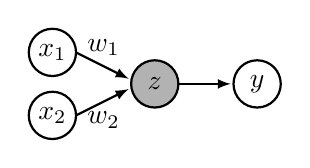
\begin{tikzpicture}[>=spaced latex]
\draw [thick, fill=white] (0,-0.4) circle [radius=0.3] node {$x_2$};
\draw [thick, fill=white] (0,0.4) circle [radius=0.3] node {$x_1$};
\draw [thick] [nn_edge] (0.3,-0.4) -- (1.0,-0.05) node[midway,below] {$w_2$};
\draw [thick] [nn_edge] (0.3,0.4) -- (1.0,0.05) node[midway,above] {$w_1$};
\draw [thick, fill=gray_neuron] (1.3,0) circle [radius=0.3] node {$z$};
\draw [thick] [nn_edge] (1.6,0) -- (2.3,0);
\draw [thick, fill=white] (2.6,0) circle [radius=0.3] node {$y$};
\end{tikzpicture}
%\end{minipage}
%}
%\end{figure}
}
}

\item When describing batches of tensors (as is commonly encountered in code), you may encounter $x_l[b,c,n,m]$ to represent an activation on layer $l$ of some network, with $b$ indexing batch element, $n$ and $m$ as spatial coordinates, and $c$ indexing channels.
\item Neuron values on layer $l$ of a deep net: $\mathbf{x}_{l}$
\item $x_{l}[n]$ refers to the $n$-th neuron on layer $l$. For neural networks with spatial feature maps (such as convolutional neural networks), each layer is an array of neurons, and we will use notation such as $x_{l}[n,m]$ to index the neuron at location $n,m$.
%\item For a network with spatial feature maps (e.g., a convolutional neural network), $x_{l}[c,i,j]$ refers to the $cij$-th neuron on layer $l$, where $i$ and $j$ index spatial position in a feature map, and $c$ indexes the channel.
\item The layer $l$ neural representation of the $i$-th datapoint in a dataset is written as $\mathbf{x}^{(i)}_{l}$.
\item We will also use $\xin$ and $\xout$ when we are describing a particular layer or module in a neural net and wish to speak of its inputs and outputs without having to keep track of layer indices.
\item For signals with multiple channels, including neural network feature maps, the first dimension of the tensor indexes over channel. For example, in $\mathbf{x} \in \mathbb{R}^{C \times N \times M \times \ldots}$, where $C$ is the number of channels of the signal.
\item For transformers, we deviate from the previous point slightly, in order to match standard notation: a set of tokens (which will be defined in the transformers chapter) is represented by a $[N \times d]$ matrix, where $d$ is the token dimensionality.
\end{itemize}


\subsection*{Probabilities}

We will sometimes not distinguish between random variables and realizations of those variables; which we mean should be clear from context. When it is important to make a distinction, we will use nonbold capital letters to refer to random variables and lowercase to refer to realizations.

Suppose $X, Y$ are discrete random variables and $\mathbf{x}, \mathbf{y}$ are realizations of those variables. $X$ and $Y$ may take on values in the sets $\mathcal{X}$ and $\mathcal{Y}$, respectively.
\begin{itemize}
    \item $a = p(X = \mathbf{x} \given \ldots)$ is the probability of the realization $X = \mathbf{x}$, possibly conditioned on some observations ($a$ is a scalar).
    \item $f = p(X \given \ldots)$ is the probability distribution over $X$, possibly conditioned on some observations ($f$ is a function: $f: \mathcal{X} \rightarrow \mathbb{R}$). If $\mathcal{X}$ is discrete, $f$ is the \emph{probability mass function}. If $\mathcal{X}$ is continuous, $f$ is the \emph{probability density function}.
    %\item $a = p(X = x | \overset{R}{y} = y)$ is the probability of the realization $\overset{R}{x}=x$ given $\overset{R}{y}=y$ ($a$ is a scalar).
    %\item $f = p(\overset{R}{x} | \overset{R}{y} = y)$ is the probability distribution over $\overset{R}{x}$ given $\overset{R}{y}=y$ ($f: \mathcal{X} \rightarrow \mathbb{R}$).
    %\item $f = p(\overset{R}{x} = x | \overset{R}{y})$ is a function with the property $f(y) = p(\overset{R}{x} = x | \overset{R}{y} = y)$ ($f: \mathcal{Y} \rightarrow \mathbb{R}$).
    %\item $p(\overset{R}{x} | \overset{R}{y})$ is the conditional probability distribution of $\overset{R}{x}$ given $\overset{R}{y}$ ($f: \mathcal{X} \times \mathcal{Y} \rightarrow \mathbb{R}$).
    %\item $p(x)$ is shorthand for $p(\overset{R}{x} = x)$.
    %\item $p(x|y)$ is shorthand for $p(\overset{R}{x} = x | \overset{R}{y} = y)$.
    %\item Suppose we have defined a named distribution, e.g., $p_{\theta}$; then referring to $p_{\theta}$ on its own is shorthand for $p(\overset{R}{x})$. This often comes up in expressions like $x \sim p_{\theta}$, which refers to $\overset{R}{x}$ as being distributed as $p_{\theta}(\overset{R}{x})$.
    %\item $p(\overset{R}{x} | y)$ is shorthand for $p(\overset{R}{x} | \overset{R}{y} = y)$
    \item $p(\mathbf{x} \given \ldots)$ is shorthand for $p(X = \mathbf{x} \given \ldots)$.
    %\item $p(\ldots | y)$ is shorthand for $p(\ldots | \overset{R}{y} = y)$.
    and so forth, following these patterns.
    \item Suppose we have defined a named distribution, for example, $p_{\theta}$, for some random variable $X$; then referring to $p_{\theta}$ on its own is shorthand for $p_{\theta}(X)$.
    \item We will write $Z \sim p$ to indicate a random variable whose distribution is $p$, and we will write $z \sim p$ to indicate a sampled realization of such a variable.
\end{itemize}
For continuous random variables, all the above notations hold except that they refer to probability densities and probability density functions rather than probabilities and probability distributions. We will sometimes also use the term ``probability distribution'' for continuous random variables, and in those cases it should be understood that we are referring to a probability density function.


\subsection*{Matrix Calculus Conventions}
\label{appendix:matrix_calc:notational_conventions}

In this book, we adopt the following conventions for matrix calculus. These conventions make the equations simpler, and that also means simpler implementations when it comes to actually writing these equations in code. Everything in this section is just definitions. There is no right or wrong to it. We could have used other conventions but we will see that these are useful ones.

Vectors are represented as column vectors with shape $[N \times 1]$:
\begin{align}
    \mathbf{x} = 
    \begin{bmatrix}
    x_1  \\
    x_2  \\
    \vdots \\
    x_N \\
    \end{bmatrix}
\end{align}
If $y$ is a scalar and $\mathbf{x}$ is an $N$-dimensional vector, then the gradient $\frac{\partial y}{\partial \mathbf{x}}$ is a row vector of shape  $[1 \times N]$:
\begin{align}
    \frac{\partial y}{\partial \mathbf{x}} =  
\begin{bmatrix}
    \frac{\partial y}{\partial x_1} & \frac{\partial y}{\partial x_2} & \cdots & \frac{\partial y}{\partial x_N} \label{backprop:scalar_vector_deriv}
\end{bmatrix}
\end{align}
If $\mathbf{y}$ is an $M$-dimensional vector and $\mathbf{x}$ is a $N$-dimensional vector then the gradient (also called the Jacobian in this case) is shaped as $[M \times N]$:
\begin{align}
\frac{\partial \mathbf{y}}{\partial \mathbf{x}} =  
\begin{bmatrix}
    \frac{\partial y_1}{\partial x_1} & \frac{\partial y_1}{\partial x_2} & \cdots & \frac{\partial y_1}{\partial x_N} \\
    \vdots & \vdots & \vdots & \vdots \\
    \frac{\partial y_M}{\partial x_1} & \frac{\partial y_M}{\partial x_2} & \cdots & \frac{\partial y_M}{\partial x_N}
\end{bmatrix}
\end{align}


Finally, if $\mathbf{W}$ is an $[N \times M]$ dimensional matrix, and $\mathcal{L}$ is a scalar, then the gradient $\frac{\partial \mathcal{L}}{\mathbf{W}}$ is represented as an $[M \times N]$ dimensional matrix (note that the dimensions are transposed from what you might have expected; this makes the math simpler later):
\begin{align}
    \frac{\partial \mathcal{L}}{\partial \mathbf{W}} &= 
        \begin{bmatrix}
            \frac{\partial \mathcal{L}}{\partial \mathbf{W}_{11}} & \ldots & \frac{\partial \mathcal{L}}{\partial \mathbf{W}_{N1}} \\
            \vdots & \ddots & \vdots \\
            \frac{\partial \mathcal{L}}{\partial \mathbf{W}_{1M}} & \ldots & \frac{\partial \mathcal{L}}{\partial \mathbf{W}_{NM}} \\
        \end{bmatrix} \label{backprop:scalar_matrix_deriv}
\end{align}
\marginnote{
We will often draw matrices and vectors to help visualize the operations. For example, if $N=3$ and $M=4$:\\[2pt]
\centerline{
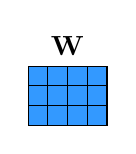
\begin{tikzpicture}
\draw[step=0.25cm,draw=black,fill=param_color_dark] (1.5,0) grid (2.5,-0.75) rectangle (1.5,0); \node at (2.0,0.25) {$\mathbf{W}$};
\end{tikzpicture}}
then, the gradient will have the form:\\[2pt]
\centerline{
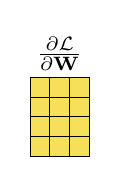
\begin{tikzpicture}
\draw[step=0.25cm,draw=black,fill=comp_graph_param_grad_bcolor] (0,0) grid (0.75,-1.0) rectangle (0,0); \node at (0.375,0.3) {$\frac{\partial \mathcal{L}}{\partial \mathbf{W}}$};
\end{tikzpicture}}
}[-.9in]

\subsection*{Conventions That Will Not Be Strictly Observed}
\begin{itemize}
\item We will often use $\mathbf{x}$ as the input to a function, and $\mathbf{y}$ as the output.
\item $f$, $g$, and $h$ are typically functions. The corresponding function spaces are $\mathcal{F}$, $\mathcal{G}$, $\mathcal{H}$.
\item Basis functions are $\phi$ and $\psi$.
\end{itemize}

\subsection*{Miscellaneous}
\begin{itemize}
\item The word ``dimension'' has two usages in the computational sciences. The first usage is as a coordinate in a multivariate data structure, for example, ``the $i$-th dimension of a vector'' or ``a 128-dimensional feature space.'' The second usage is as the shape of a multidimensional array, as in ``a 4D tensor.'' We will use both these meanings in this book and we hope the usage will be clear from context.
\end{itemize}


\mainmatter
\cleardoublepage
%\maketitle
%\tableofcontents

%\listoffigures
%\listoftables

%   
\chapter*{Notation}
\addcontentsline{toc}{fmbm}{Notation}
\addtocontents{toc}{\protect\enlargethispage{1\baselineskip}}

\marginnote{We will use notes inside boxes to bring attention to important concepts, or to add additional comments without breaking the flow of the main text.}
This book deals with many different fields and each has its own notation. We will stick to the following conventions throughout most of this book, and indicate when we deviate from these rules. To define the conventions we give examples of usage, from which you can infer the pattern.

\subsection*{General Notation}
\begin{itemize}
\item Scalar: $x$, $y$, $z$.
\item Vector: $\mathbf{x}, \mathbf{y}, \mathbf{z}$. We use bold letters to represent vectors, matrices, and tensors.
\item Index of a vector: $x_i$, $x_j$, $y_i$, or $x[i]$, $x[j]$, $y[i]$.
\item Matrix: $\mathbf{X}$, $\mathbf{Y}$, $\mathbf{Z}$. We use bold letters to represent vectors, matrices, and tensors.
\item Index of a matrix: $X_{ij}$, $Y_{jk}$, $Z_{ii}$, or $X[i,j]$, $Y[j,k]$, $Z[i,i]$.
\item For an indexed matrix $X_{ij}$ or $X[i,j]$, $i$ indexes rows and $j$ indexes columns. We use non-bold font because $X_{ij}$ and $X[i,j]$ are scalars.
\item Slice of a matrix: $\mathbf{X}_i$ or $\mathbf{X}[i,:]$; $\mathbf{X}[:,j]$. Here is one example, using zero-based indexing:
\begin{align*}
\mathbf{X} = 
\begin{bmatrix}
    1 & 2 \\
    3 & 4 \\
    5 & 6
\end{bmatrix}
&&
\mathbf{X}[2,:] = 
\begin{bmatrix}
    5 & 6
\end{bmatrix}
\end{align*}
\item Tensor (i.e., multidimensional arrays): Typically, we will use lowercase bold variables to represent tensors, for example, $\mathbf{x}$. This is because tensors can have any number of dimensions (they can be one-dimensional, two-dimensional, three-dimensional, and so on). Furthermore, we will often define operators that are agnostic to the dimensionality of the tensor (they apply to $N$-dimensional arrays, for any $N$). However, in some sections, we use uppercase to make a distinction between tensors of different shapes, and we will specify when this is the case. 
\marginnote{
A 3D tensor that could represent a $C \times H \times W$ color image: 
\\[6pt]
\centerline{
\includegraphics[width=.25\linewidth]{figures/neural_nets/3D_tensor_example.eps}
}
}[-0.05in]
\item Index or slice of a tensor: $x[c,i,j,k]$, $\mathbf{x}[:,:,k]$; if $\mathbf{x}$ is a multidimensional tensor and we wish to slice by the first dimension, we may use $\mathbf{x}_t$ or $\mathbf{x}[t]$ or $\mathbf{x}[t,:]$, all of which have the same meaning.
%\item When the dimensionality of a variable is arbitrary (can take on different values in different settings) we will consider it a tensor and use the tensor notation.
\item A set of $N$ datapoints: $\{x^{(i)}\}_{i=1}^N$, $\{\mathbf{x}^{(i)}\}_{i=1}^N$, $\{\mathbf{X}^{(i)}\}_{i=1}^N$
%\item $\mathbf{A} = [\mathbf{x},\mathbf{y},\mathbf{z}]$ concatenates column vectors $\mathbf{x},\mathbf{y},\mathbf{z}$ as columns of matrix $A$. $\mathbf{A} = [\mathbf{x}^\transpose,\mathbf{y}^\transpose,\mathbf{z}^\transpose]$ concatenates these vectors as rows of $\mathbf{A}$. 
\item Dot product: $\mathbf{x}^\transpose\mathbf{y}$
\item Matrix product: $\mathbf{A}\mathbf{B}$
\item Hadamard product (i.e., element-wise product): $\mathbf{x} \hadamard \mathbf{y}$, $\mathbf{A} \hadamard \mathbf{B}$
\item Product of two scalars: $ab$ or $a*b$ 
\end{itemize}
\marginnote{In the geometry chapters, and in some other chapters, the variables $x$, $y$, $z$ will denote location and will have a special treatment.}[-0.2in]


\subsection*{Signal Processing}
\begin{itemize}
\item Discrete signals (and images) are vectors $\mathbf{x}, \mathbf{y}, \mathbf{z}$.
\item When indexing a discrete signal we will use brackets: $x \left[ n\right]$, where $n$ is a discrete index.
\item Continuous signals are denoted $x (t)$, where $t$ is a continuous variable.
\item Convolution operator: $\circ$
\item Cross-correlation operator: $\star$
\item Discrete Fourier transforms: $X \left[ u\right]$, where $u$ is a discrete frequency index.
\end{itemize}

\subsection*{Images}

Images are a very special signal and, whenever is convenient, we will use the following notation:
\marginnote{We will use the letter $\img$, from $\img$ight, when the signal is an image. We use this letter because it is very distinct from all the other notation. But sometimes we will use other notation if it is more convenient.}
\begin{itemize}
\item Image as a discrete 2D signal: $\img \left[ n,m \right]$ where $n$ indexes columns and $m$ indexes rows. The origin, $n=m=0$, corresponds to the bottom-left side of the image unless we specify a different convention. An image has a size $N \times M$, $N$ columns and $M$ rows. 
\item Image as a matrix: $\boldimg$ of size $M \times N$, $M$ rows and $N$ columns, which can be indexed as $\img_{ij}$.
\item The Fourier transform on an image: $\capitalimg \left[ u,v\right]$, where $u$ and $v$ are spatial frequencies.
\end{itemize}
Note that the way matrices and images are indexed is transposed. However, we will rarely represent images as arrays. If we do, we will use the general notation and the images will be just generic signals, $\mathbf{x}, \mathbf{y}, \mathbf{z}$. 

\subsection*{Machine Learning}
\begin{itemize}
    \item Total loss function / cost function / objective function: $J$
    \item Per-datapoint loss function: $\mathcal{L}$
    \item Generic learnable parameters: $\theta$
\end{itemize}


\subsection*{Neural Networks}
\begin{itemize}
\item \textit{Parameters}: $\theta$. These include weights, $\mathbf{W}$, and biases, $\mathbf{b}$, as well as any other learnable parameters of a network.
\item \textit{Data}: $\mathbf{x}$. Data can refer to inputs to the network, activations on hidden layers, outputs from the network, and so on. Any representation of the signal being processed is considered to be data. Sometimes we will wish to distinguish between the raw inputs, hidden units, and outputs to a network, in which case we will use $\mathbf{x}$, $\mathbf{h}$, and $\mathbf{y}$ respectively. When we need to to distinguish between pre-activation hidden units and postactivation, we will use $\mathbf{z}$ for pre-activation and $\mathbf{h}$ for postactivation.
\marginnote{
%Neural net:
%~\\
%\begin{figure}
%\centerline{
%\noindent\hspace{0.05\linewidth}
%\begin{minipage}%{1\linewidth}
\centerline{
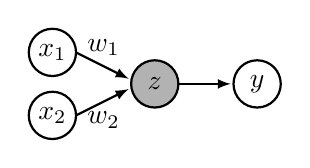
\begin{tikzpicture}[>=spaced latex]
\draw [thick, fill=white] (0,-0.4) circle [radius=0.3] node {$x_2$};
\draw [thick, fill=white] (0,0.4) circle [radius=0.3] node {$x_1$};
\draw [thick] [nn_edge] (0.3,-0.4) -- (1.0,-0.05) node[midway,below] {$w_2$};
\draw [thick] [nn_edge] (0.3,0.4) -- (1.0,0.05) node[midway,above] {$w_1$};
\draw [thick, fill=gray_neuron] (1.3,0) circle [radius=0.3] node {$z$};
\draw [thick] [nn_edge] (1.6,0) -- (2.3,0);
\draw [thick, fill=white] (2.6,0) circle [radius=0.3] node {$y$};
\end{tikzpicture}
%\end{minipage}
%}
%\end{figure}
}
}

\item When describing batches of tensors (as is commonly encountered in code), you may encounter $x_l[b,c,n,m]$ to represent an activation on layer $l$ of some network, with $b$ indexing batch element, $n$ and $m$ as spatial coordinates, and $c$ indexing channels.
\item Neuron values on layer $l$ of a deep net: $\mathbf{x}_{l}$
\item $x_{l}[n]$ refers to the $n$-th neuron on layer $l$. For neural networks with spatial feature maps (such as convolutional neural networks), each layer is an array of neurons, and we will use notation such as $x_{l}[n,m]$ to index the neuron at location $n,m$.
%\item For a network with spatial feature maps (e.g., a convolutional neural network), $x_{l}[c,i,j]$ refers to the $cij$-th neuron on layer $l$, where $i$ and $j$ index spatial position in a feature map, and $c$ indexes the channel.
\item The layer $l$ neural representation of the $i$-th datapoint in a dataset is written as $\mathbf{x}^{(i)}_{l}$.
\item We will also use $\xin$ and $\xout$ when we are describing a particular layer or module in a neural net and wish to speak of its inputs and outputs without having to keep track of layer indices.
\item For signals with multiple channels, including neural network feature maps, the first dimension of the tensor indexes over channel. For example, in $\mathbf{x} \in \mathbb{R}^{C \times N \times M \times \ldots}$, where $C$ is the number of channels of the signal.
\item For transformers, we deviate from the previous point slightly, in order to match standard notation: a set of tokens (which will be defined in the transformers chapter) is represented by a $[N \times d]$ matrix, where $d$ is the token dimensionality.
\end{itemize}


\subsection*{Probabilities}

We will sometimes not distinguish between random variables and realizations of those variables; which we mean should be clear from context. When it is important to make a distinction, we will use nonbold capital letters to refer to random variables and lowercase to refer to realizations.

Suppose $X, Y$ are discrete random variables and $\mathbf{x}, \mathbf{y}$ are realizations of those variables. $X$ and $Y$ may take on values in the sets $\mathcal{X}$ and $\mathcal{Y}$, respectively.
\begin{itemize}
    \item $a = p(X = \mathbf{x} \given \ldots)$ is the probability of the realization $X = \mathbf{x}$, possibly conditioned on some observations ($a$ is a scalar).
    \item $f = p(X \given \ldots)$ is the probability distribution over $X$, possibly conditioned on some observations ($f$ is a function: $f: \mathcal{X} \rightarrow \mathbb{R}$). If $\mathcal{X}$ is discrete, $f$ is the \emph{probability mass function}. If $\mathcal{X}$ is continuous, $f$ is the \emph{probability density function}.
    %\item $a = p(X = x | \overset{R}{y} = y)$ is the probability of the realization $\overset{R}{x}=x$ given $\overset{R}{y}=y$ ($a$ is a scalar).
    %\item $f = p(\overset{R}{x} | \overset{R}{y} = y)$ is the probability distribution over $\overset{R}{x}$ given $\overset{R}{y}=y$ ($f: \mathcal{X} \rightarrow \mathbb{R}$).
    %\item $f = p(\overset{R}{x} = x | \overset{R}{y})$ is a function with the property $f(y) = p(\overset{R}{x} = x | \overset{R}{y} = y)$ ($f: \mathcal{Y} \rightarrow \mathbb{R}$).
    %\item $p(\overset{R}{x} | \overset{R}{y})$ is the conditional probability distribution of $\overset{R}{x}$ given $\overset{R}{y}$ ($f: \mathcal{X} \times \mathcal{Y} \rightarrow \mathbb{R}$).
    %\item $p(x)$ is shorthand for $p(\overset{R}{x} = x)$.
    %\item $p(x|y)$ is shorthand for $p(\overset{R}{x} = x | \overset{R}{y} = y)$.
    %\item Suppose we have defined a named distribution, e.g., $p_{\theta}$; then referring to $p_{\theta}$ on its own is shorthand for $p(\overset{R}{x})$. This often comes up in expressions like $x \sim p_{\theta}$, which refers to $\overset{R}{x}$ as being distributed as $p_{\theta}(\overset{R}{x})$.
    %\item $p(\overset{R}{x} | y)$ is shorthand for $p(\overset{R}{x} | \overset{R}{y} = y)$
    \item $p(\mathbf{x} \given \ldots)$ is shorthand for $p(X = \mathbf{x} \given \ldots)$.
    %\item $p(\ldots | y)$ is shorthand for $p(\ldots | \overset{R}{y} = y)$.
    and so forth, following these patterns.
    \item Suppose we have defined a named distribution, for example, $p_{\theta}$, for some random variable $X$; then referring to $p_{\theta}$ on its own is shorthand for $p_{\theta}(X)$.
    \item We will write $Z \sim p$ to indicate a random variable whose distribution is $p$, and we will write $z \sim p$ to indicate a sampled realization of such a variable.
\end{itemize}
For continuous random variables, all the above notations hold except that they refer to probability densities and probability density functions rather than probabilities and probability distributions. We will sometimes also use the term ``probability distribution'' for continuous random variables, and in those cases it should be understood that we are referring to a probability density function.


\subsection*{Matrix Calculus Conventions}
\label{appendix:matrix_calc:notational_conventions}

In this book, we adopt the following conventions for matrix calculus. These conventions make the equations simpler, and that also means simpler implementations when it comes to actually writing these equations in code. Everything in this section is just definitions. There is no right or wrong to it. We could have used other conventions but we will see that these are useful ones.

Vectors are represented as column vectors with shape $[N \times 1]$:
\begin{align}
    \mathbf{x} = 
    \begin{bmatrix}
    x_1  \\
    x_2  \\
    \vdots \\
    x_N \\
    \end{bmatrix}
\end{align}
If $y$ is a scalar and $\mathbf{x}$ is an $N$-dimensional vector, then the gradient $\frac{\partial y}{\partial \mathbf{x}}$ is a row vector of shape  $[1 \times N]$:
\begin{align}
    \frac{\partial y}{\partial \mathbf{x}} =  
\begin{bmatrix}
    \frac{\partial y}{\partial x_1} & \frac{\partial y}{\partial x_2} & \cdots & \frac{\partial y}{\partial x_N} \label{backprop:scalar_vector_deriv}
\end{bmatrix}
\end{align}
If $\mathbf{y}$ is an $M$-dimensional vector and $\mathbf{x}$ is a $N$-dimensional vector then the gradient (also called the Jacobian in this case) is shaped as $[M \times N]$:
\begin{align}
\frac{\partial \mathbf{y}}{\partial \mathbf{x}} =  
\begin{bmatrix}
    \frac{\partial y_1}{\partial x_1} & \frac{\partial y_1}{\partial x_2} & \cdots & \frac{\partial y_1}{\partial x_N} \\
    \vdots & \vdots & \vdots & \vdots \\
    \frac{\partial y_M}{\partial x_1} & \frac{\partial y_M}{\partial x_2} & \cdots & \frac{\partial y_M}{\partial x_N}
\end{bmatrix}
\end{align}


Finally, if $\mathbf{W}$ is an $[N \times M]$ dimensional matrix, and $\mathcal{L}$ is a scalar, then the gradient $\frac{\partial \mathcal{L}}{\mathbf{W}}$ is represented as an $[M \times N]$ dimensional matrix (note that the dimensions are transposed from what you might have expected; this makes the math simpler later):
\begin{align}
    \frac{\partial \mathcal{L}}{\partial \mathbf{W}} &= 
        \begin{bmatrix}
            \frac{\partial \mathcal{L}}{\partial \mathbf{W}_{11}} & \ldots & \frac{\partial \mathcal{L}}{\partial \mathbf{W}_{N1}} \\
            \vdots & \ddots & \vdots \\
            \frac{\partial \mathcal{L}}{\partial \mathbf{W}_{1M}} & \ldots & \frac{\partial \mathcal{L}}{\partial \mathbf{W}_{NM}} \\
        \end{bmatrix} \label{backprop:scalar_matrix_deriv}
\end{align}
\marginnote{
We will often draw matrices and vectors to help visualize the operations. For example, if $N=3$ and $M=4$:\\[2pt]
\centerline{
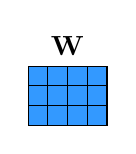
\begin{tikzpicture}
\draw[step=0.25cm,draw=black,fill=param_color_dark] (1.5,0) grid (2.5,-0.75) rectangle (1.5,0); \node at (2.0,0.25) {$\mathbf{W}$};
\end{tikzpicture}}
then, the gradient will have the form:\\[2pt]
\centerline{
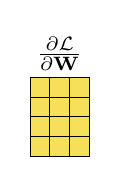
\begin{tikzpicture}
\draw[step=0.25cm,draw=black,fill=comp_graph_param_grad_bcolor] (0,0) grid (0.75,-1.0) rectangle (0,0); \node at (0.375,0.3) {$\frac{\partial \mathcal{L}}{\partial \mathbf{W}}$};
\end{tikzpicture}}
}[-.9in]

\subsection*{Conventions That Will Not Be Strictly Observed}
\begin{itemize}
\item We will often use $\mathbf{x}$ as the input to a function, and $\mathbf{y}$ as the output.
\item $f$, $g$, and $h$ are typically functions. The corresponding function spaces are $\mathcal{F}$, $\mathcal{G}$, $\mathcal{H}$.
\item Basis functions are $\phi$ and $\psi$.
\end{itemize}

\subsection*{Miscellaneous}
\begin{itemize}
\item The word ``dimension'' has two usages in the computational sciences. The first usage is as a coordinate in a multivariate data structure, for example, ``the $i$-th dimension of a vector'' or ``a 128-dimensional feature space.'' The second usage is as the shape of a multidimensional array, as in ``a 4D tensor.'' We will use both these meanings in this book and we hope the usage will be clear from context.
\end{itemize}



%%%%%%%%%%%%%%%%%%%%%%%%%%%%%%%%%%%%%%
%% CHAPTERS:

%\setcounter{chapter}{0}

%   
\chapter*{Notation}
\addcontentsline{toc}{fmbm}{Notation}
\addtocontents{toc}{\protect\enlargethispage{1\baselineskip}}

\marginnote{We will use notes inside boxes to bring attention to important concepts, or to add additional comments without breaking the flow of the main text.}
This book deals with many different fields and each has its own notation. We will stick to the following conventions throughout most of this book, and indicate when we deviate from these rules. To define the conventions we give examples of usage, from which you can infer the pattern.

\subsection*{General Notation}
\begin{itemize}
\item Scalar: $x$, $y$, $z$.
\item Vector: $\mathbf{x}, \mathbf{y}, \mathbf{z}$. We use bold letters to represent vectors, matrices, and tensors.
\item Index of a vector: $x_i$, $x_j$, $y_i$, or $x[i]$, $x[j]$, $y[i]$.
\item Matrix: $\mathbf{X}$, $\mathbf{Y}$, $\mathbf{Z}$. We use bold letters to represent vectors, matrices, and tensors.
\item Index of a matrix: $X_{ij}$, $Y_{jk}$, $Z_{ii}$, or $X[i,j]$, $Y[j,k]$, $Z[i,i]$.
\item For an indexed matrix $X_{ij}$ or $X[i,j]$, $i$ indexes rows and $j$ indexes columns. We use non-bold font because $X_{ij}$ and $X[i,j]$ are scalars.
\item Slice of a matrix: $\mathbf{X}_i$ or $\mathbf{X}[i,:]$; $\mathbf{X}[:,j]$. Here is one example, using zero-based indexing:
\begin{align*}
\mathbf{X} = 
\begin{bmatrix}
    1 & 2 \\
    3 & 4 \\
    5 & 6
\end{bmatrix}
&&
\mathbf{X}[2,:] = 
\begin{bmatrix}
    5 & 6
\end{bmatrix}
\end{align*}
\item Tensor (i.e., multidimensional arrays): Typically, we will use lowercase bold variables to represent tensors, for example, $\mathbf{x}$. This is because tensors can have any number of dimensions (they can be one-dimensional, two-dimensional, three-dimensional, and so on). Furthermore, we will often define operators that are agnostic to the dimensionality of the tensor (they apply to $N$-dimensional arrays, for any $N$). However, in some sections, we use uppercase to make a distinction between tensors of different shapes, and we will specify when this is the case. 
\marginnote{
A 3D tensor that could represent a $C \times H \times W$ color image: 
\\[6pt]
\centerline{
\includegraphics[width=.25\linewidth]{figures/neural_nets/3D_tensor_example.eps}
}
}[-0.05in]
\item Index or slice of a tensor: $x[c,i,j,k]$, $\mathbf{x}[:,:,k]$; if $\mathbf{x}$ is a multidimensional tensor and we wish to slice by the first dimension, we may use $\mathbf{x}_t$ or $\mathbf{x}[t]$ or $\mathbf{x}[t,:]$, all of which have the same meaning.
%\item When the dimensionality of a variable is arbitrary (can take on different values in different settings) we will consider it a tensor and use the tensor notation.
\item A set of $N$ datapoints: $\{x^{(i)}\}_{i=1}^N$, $\{\mathbf{x}^{(i)}\}_{i=1}^N$, $\{\mathbf{X}^{(i)}\}_{i=1}^N$
%\item $\mathbf{A} = [\mathbf{x},\mathbf{y},\mathbf{z}]$ concatenates column vectors $\mathbf{x},\mathbf{y},\mathbf{z}$ as columns of matrix $A$. $\mathbf{A} = [\mathbf{x}^\transpose,\mathbf{y}^\transpose,\mathbf{z}^\transpose]$ concatenates these vectors as rows of $\mathbf{A}$. 
\item Dot product: $\mathbf{x}^\transpose\mathbf{y}$
\item Matrix product: $\mathbf{A}\mathbf{B}$
\item Hadamard product (i.e., element-wise product): $\mathbf{x} \hadamard \mathbf{y}$, $\mathbf{A} \hadamard \mathbf{B}$
\item Product of two scalars: $ab$ or $a*b$ 
\end{itemize}
\marginnote{In the geometry chapters, and in some other chapters, the variables $x$, $y$, $z$ will denote location and will have a special treatment.}[-0.2in]


\subsection*{Signal Processing}
\begin{itemize}
\item Discrete signals (and images) are vectors $\mathbf{x}, \mathbf{y}, \mathbf{z}$.
\item When indexing a discrete signal we will use brackets: $x \left[ n\right]$, where $n$ is a discrete index.
\item Continuous signals are denoted $x (t)$, where $t$ is a continuous variable.
\item Convolution operator: $\circ$
\item Cross-correlation operator: $\star$
\item Discrete Fourier transforms: $X \left[ u\right]$, where $u$ is a discrete frequency index.
\end{itemize}

\subsection*{Images}

Images are a very special signal and, whenever is convenient, we will use the following notation:
\marginnote{We will use the letter $\img$, from $\img$ight, when the signal is an image. We use this letter because it is very distinct from all the other notation. But sometimes we will use other notation if it is more convenient.}
\begin{itemize}
\item Image as a discrete 2D signal: $\img \left[ n,m \right]$ where $n$ indexes columns and $m$ indexes rows. The origin, $n=m=0$, corresponds to the bottom-left side of the image unless we specify a different convention. An image has a size $N \times M$, $N$ columns and $M$ rows. 
\item Image as a matrix: $\boldimg$ of size $M \times N$, $M$ rows and $N$ columns, which can be indexed as $\img_{ij}$.
\item The Fourier transform on an image: $\capitalimg \left[ u,v\right]$, where $u$ and $v$ are spatial frequencies.
\end{itemize}
Note that the way matrices and images are indexed is transposed. However, we will rarely represent images as arrays. If we do, we will use the general notation and the images will be just generic signals, $\mathbf{x}, \mathbf{y}, \mathbf{z}$. 

\subsection*{Machine Learning}
\begin{itemize}
    \item Total loss function / cost function / objective function: $J$
    \item Per-datapoint loss function: $\mathcal{L}$
    \item Generic learnable parameters: $\theta$
\end{itemize}


\subsection*{Neural Networks}
\begin{itemize}
\item \textit{Parameters}: $\theta$. These include weights, $\mathbf{W}$, and biases, $\mathbf{b}$, as well as any other learnable parameters of a network.
\item \textit{Data}: $\mathbf{x}$. Data can refer to inputs to the network, activations on hidden layers, outputs from the network, and so on. Any representation of the signal being processed is considered to be data. Sometimes we will wish to distinguish between the raw inputs, hidden units, and outputs to a network, in which case we will use $\mathbf{x}$, $\mathbf{h}$, and $\mathbf{y}$ respectively. When we need to to distinguish between pre-activation hidden units and postactivation, we will use $\mathbf{z}$ for pre-activation and $\mathbf{h}$ for postactivation.
\marginnote{
%Neural net:
%~\\
%\begin{figure}
%\centerline{
%\noindent\hspace{0.05\linewidth}
%\begin{minipage}%{1\linewidth}
\centerline{
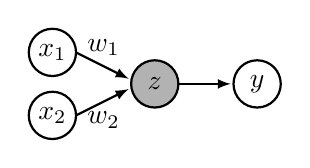
\begin{tikzpicture}[>=spaced latex]
\draw [thick, fill=white] (0,-0.4) circle [radius=0.3] node {$x_2$};
\draw [thick, fill=white] (0,0.4) circle [radius=0.3] node {$x_1$};
\draw [thick] [nn_edge] (0.3,-0.4) -- (1.0,-0.05) node[midway,below] {$w_2$};
\draw [thick] [nn_edge] (0.3,0.4) -- (1.0,0.05) node[midway,above] {$w_1$};
\draw [thick, fill=gray_neuron] (1.3,0) circle [radius=0.3] node {$z$};
\draw [thick] [nn_edge] (1.6,0) -- (2.3,0);
\draw [thick, fill=white] (2.6,0) circle [radius=0.3] node {$y$};
\end{tikzpicture}
%\end{minipage}
%}
%\end{figure}
}
}

\item When describing batches of tensors (as is commonly encountered in code), you may encounter $x_l[b,c,n,m]$ to represent an activation on layer $l$ of some network, with $b$ indexing batch element, $n$ and $m$ as spatial coordinates, and $c$ indexing channels.
\item Neuron values on layer $l$ of a deep net: $\mathbf{x}_{l}$
\item $x_{l}[n]$ refers to the $n$-th neuron on layer $l$. For neural networks with spatial feature maps (such as convolutional neural networks), each layer is an array of neurons, and we will use notation such as $x_{l}[n,m]$ to index the neuron at location $n,m$.
%\item For a network with spatial feature maps (e.g., a convolutional neural network), $x_{l}[c,i,j]$ refers to the $cij$-th neuron on layer $l$, where $i$ and $j$ index spatial position in a feature map, and $c$ indexes the channel.
\item The layer $l$ neural representation of the $i$-th datapoint in a dataset is written as $\mathbf{x}^{(i)}_{l}$.
\item We will also use $\xin$ and $\xout$ when we are describing a particular layer or module in a neural net and wish to speak of its inputs and outputs without having to keep track of layer indices.
\item For signals with multiple channels, including neural network feature maps, the first dimension of the tensor indexes over channel. For example, in $\mathbf{x} \in \mathbb{R}^{C \times N \times M \times \ldots}$, where $C$ is the number of channels of the signal.
\item For transformers, we deviate from the previous point slightly, in order to match standard notation: a set of tokens (which will be defined in the transformers chapter) is represented by a $[N \times d]$ matrix, where $d$ is the token dimensionality.
\end{itemize}


\subsection*{Probabilities}

We will sometimes not distinguish between random variables and realizations of those variables; which we mean should be clear from context. When it is important to make a distinction, we will use nonbold capital letters to refer to random variables and lowercase to refer to realizations.

Suppose $X, Y$ are discrete random variables and $\mathbf{x}, \mathbf{y}$ are realizations of those variables. $X$ and $Y$ may take on values in the sets $\mathcal{X}$ and $\mathcal{Y}$, respectively.
\begin{itemize}
    \item $a = p(X = \mathbf{x} \given \ldots)$ is the probability of the realization $X = \mathbf{x}$, possibly conditioned on some observations ($a$ is a scalar).
    \item $f = p(X \given \ldots)$ is the probability distribution over $X$, possibly conditioned on some observations ($f$ is a function: $f: \mathcal{X} \rightarrow \mathbb{R}$). If $\mathcal{X}$ is discrete, $f$ is the \emph{probability mass function}. If $\mathcal{X}$ is continuous, $f$ is the \emph{probability density function}.
    %\item $a = p(X = x | \overset{R}{y} = y)$ is the probability of the realization $\overset{R}{x}=x$ given $\overset{R}{y}=y$ ($a$ is a scalar).
    %\item $f = p(\overset{R}{x} | \overset{R}{y} = y)$ is the probability distribution over $\overset{R}{x}$ given $\overset{R}{y}=y$ ($f: \mathcal{X} \rightarrow \mathbb{R}$).
    %\item $f = p(\overset{R}{x} = x | \overset{R}{y})$ is a function with the property $f(y) = p(\overset{R}{x} = x | \overset{R}{y} = y)$ ($f: \mathcal{Y} \rightarrow \mathbb{R}$).
    %\item $p(\overset{R}{x} | \overset{R}{y})$ is the conditional probability distribution of $\overset{R}{x}$ given $\overset{R}{y}$ ($f: \mathcal{X} \times \mathcal{Y} \rightarrow \mathbb{R}$).
    %\item $p(x)$ is shorthand for $p(\overset{R}{x} = x)$.
    %\item $p(x|y)$ is shorthand for $p(\overset{R}{x} = x | \overset{R}{y} = y)$.
    %\item Suppose we have defined a named distribution, e.g., $p_{\theta}$; then referring to $p_{\theta}$ on its own is shorthand for $p(\overset{R}{x})$. This often comes up in expressions like $x \sim p_{\theta}$, which refers to $\overset{R}{x}$ as being distributed as $p_{\theta}(\overset{R}{x})$.
    %\item $p(\overset{R}{x} | y)$ is shorthand for $p(\overset{R}{x} | \overset{R}{y} = y)$
    \item $p(\mathbf{x} \given \ldots)$ is shorthand for $p(X = \mathbf{x} \given \ldots)$.
    %\item $p(\ldots | y)$ is shorthand for $p(\ldots | \overset{R}{y} = y)$.
    and so forth, following these patterns.
    \item Suppose we have defined a named distribution, for example, $p_{\theta}$, for some random variable $X$; then referring to $p_{\theta}$ on its own is shorthand for $p_{\theta}(X)$.
    \item We will write $Z \sim p$ to indicate a random variable whose distribution is $p$, and we will write $z \sim p$ to indicate a sampled realization of such a variable.
\end{itemize}
For continuous random variables, all the above notations hold except that they refer to probability densities and probability density functions rather than probabilities and probability distributions. We will sometimes also use the term ``probability distribution'' for continuous random variables, and in those cases it should be understood that we are referring to a probability density function.


\subsection*{Matrix Calculus Conventions}
\label{appendix:matrix_calc:notational_conventions}

In this book, we adopt the following conventions for matrix calculus. These conventions make the equations simpler, and that also means simpler implementations when it comes to actually writing these equations in code. Everything in this section is just definitions. There is no right or wrong to it. We could have used other conventions but we will see that these are useful ones.

Vectors are represented as column vectors with shape $[N \times 1]$:
\begin{align}
    \mathbf{x} = 
    \begin{bmatrix}
    x_1  \\
    x_2  \\
    \vdots \\
    x_N \\
    \end{bmatrix}
\end{align}
If $y$ is a scalar and $\mathbf{x}$ is an $N$-dimensional vector, then the gradient $\frac{\partial y}{\partial \mathbf{x}}$ is a row vector of shape  $[1 \times N]$:
\begin{align}
    \frac{\partial y}{\partial \mathbf{x}} =  
\begin{bmatrix}
    \frac{\partial y}{\partial x_1} & \frac{\partial y}{\partial x_2} & \cdots & \frac{\partial y}{\partial x_N} \label{backprop:scalar_vector_deriv}
\end{bmatrix}
\end{align}
If $\mathbf{y}$ is an $M$-dimensional vector and $\mathbf{x}$ is a $N$-dimensional vector then the gradient (also called the Jacobian in this case) is shaped as $[M \times N]$:
\begin{align}
\frac{\partial \mathbf{y}}{\partial \mathbf{x}} =  
\begin{bmatrix}
    \frac{\partial y_1}{\partial x_1} & \frac{\partial y_1}{\partial x_2} & \cdots & \frac{\partial y_1}{\partial x_N} \\
    \vdots & \vdots & \vdots & \vdots \\
    \frac{\partial y_M}{\partial x_1} & \frac{\partial y_M}{\partial x_2} & \cdots & \frac{\partial y_M}{\partial x_N}
\end{bmatrix}
\end{align}


Finally, if $\mathbf{W}$ is an $[N \times M]$ dimensional matrix, and $\mathcal{L}$ is a scalar, then the gradient $\frac{\partial \mathcal{L}}{\mathbf{W}}$ is represented as an $[M \times N]$ dimensional matrix (note that the dimensions are transposed from what you might have expected; this makes the math simpler later):
\begin{align}
    \frac{\partial \mathcal{L}}{\partial \mathbf{W}} &= 
        \begin{bmatrix}
            \frac{\partial \mathcal{L}}{\partial \mathbf{W}_{11}} & \ldots & \frac{\partial \mathcal{L}}{\partial \mathbf{W}_{N1}} \\
            \vdots & \ddots & \vdots \\
            \frac{\partial \mathcal{L}}{\partial \mathbf{W}_{1M}} & \ldots & \frac{\partial \mathcal{L}}{\partial \mathbf{W}_{NM}} \\
        \end{bmatrix} \label{backprop:scalar_matrix_deriv}
\end{align}
\marginnote{
We will often draw matrices and vectors to help visualize the operations. For example, if $N=3$ and $M=4$:\\[2pt]
\centerline{
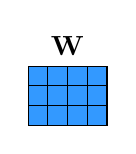
\begin{tikzpicture}
\draw[step=0.25cm,draw=black,fill=param_color_dark] (1.5,0) grid (2.5,-0.75) rectangle (1.5,0); \node at (2.0,0.25) {$\mathbf{W}$};
\end{tikzpicture}}
then, the gradient will have the form:\\[2pt]
\centerline{
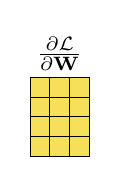
\begin{tikzpicture}
\draw[step=0.25cm,draw=black,fill=comp_graph_param_grad_bcolor] (0,0) grid (0.75,-1.0) rectangle (0,0); \node at (0.375,0.3) {$\frac{\partial \mathcal{L}}{\partial \mathbf{W}}$};
\end{tikzpicture}}
}[-.9in]

\subsection*{Conventions That Will Not Be Strictly Observed}
\begin{itemize}
\item We will often use $\mathbf{x}$ as the input to a function, and $\mathbf{y}$ as the output.
\item $f$, $g$, and $h$ are typically functions. The corresponding function spaces are $\mathcal{F}$, $\mathcal{G}$, $\mathcal{H}$.
\item Basis functions are $\phi$ and $\psi$.
\end{itemize}

\subsection*{Miscellaneous}
\begin{itemize}
\item The word ``dimension'' has two usages in the computational sciences. The first usage is as a coordinate in a multivariate data structure, for example, ``the $i$-th dimension of a vector'' or ``a 128-dimensional feature space.'' The second usage is as the shape of a multidimensional array, as in ``a 4D tensor.'' We will use both these meanings in this book and we hope the usage will be clear from context.
\end{itemize}



%\part{Learning}
%\setcounter{chapter}{13}
% \include{parts/part_foundation_learning}
% 
%\setcounter{chapter}{6}

\chapter{Introduction to Learning}
\label{chapter:intro_to_learning}

\section{Introduction}
The goal of learning is to extract lessons from past experience in order to solve future problems. Typically, this involves searching for an algorithm that solves past instances of the problem. This algorithm can then be applied to future instances of the problem.

\marginnote{Past and future do not necessarily refer to the calendar date; instead they refer to what the \textit{learner} has previously seen and what the learner will see next.}[-1.4cm]
%\marginnote{An {\bf algorithm} is a formal mapping from inputs to outputs, e.g., from a problem statement to its solution.}[-0.83cm]

Because learning is itself an algorithm, it can be understood as a meta-algorithm: an algorithm that outputs algorithms (\fig{\ref{fig:learning_as_meta_algorithm}}).

\begin{figure}[h!]
    \centerline{
    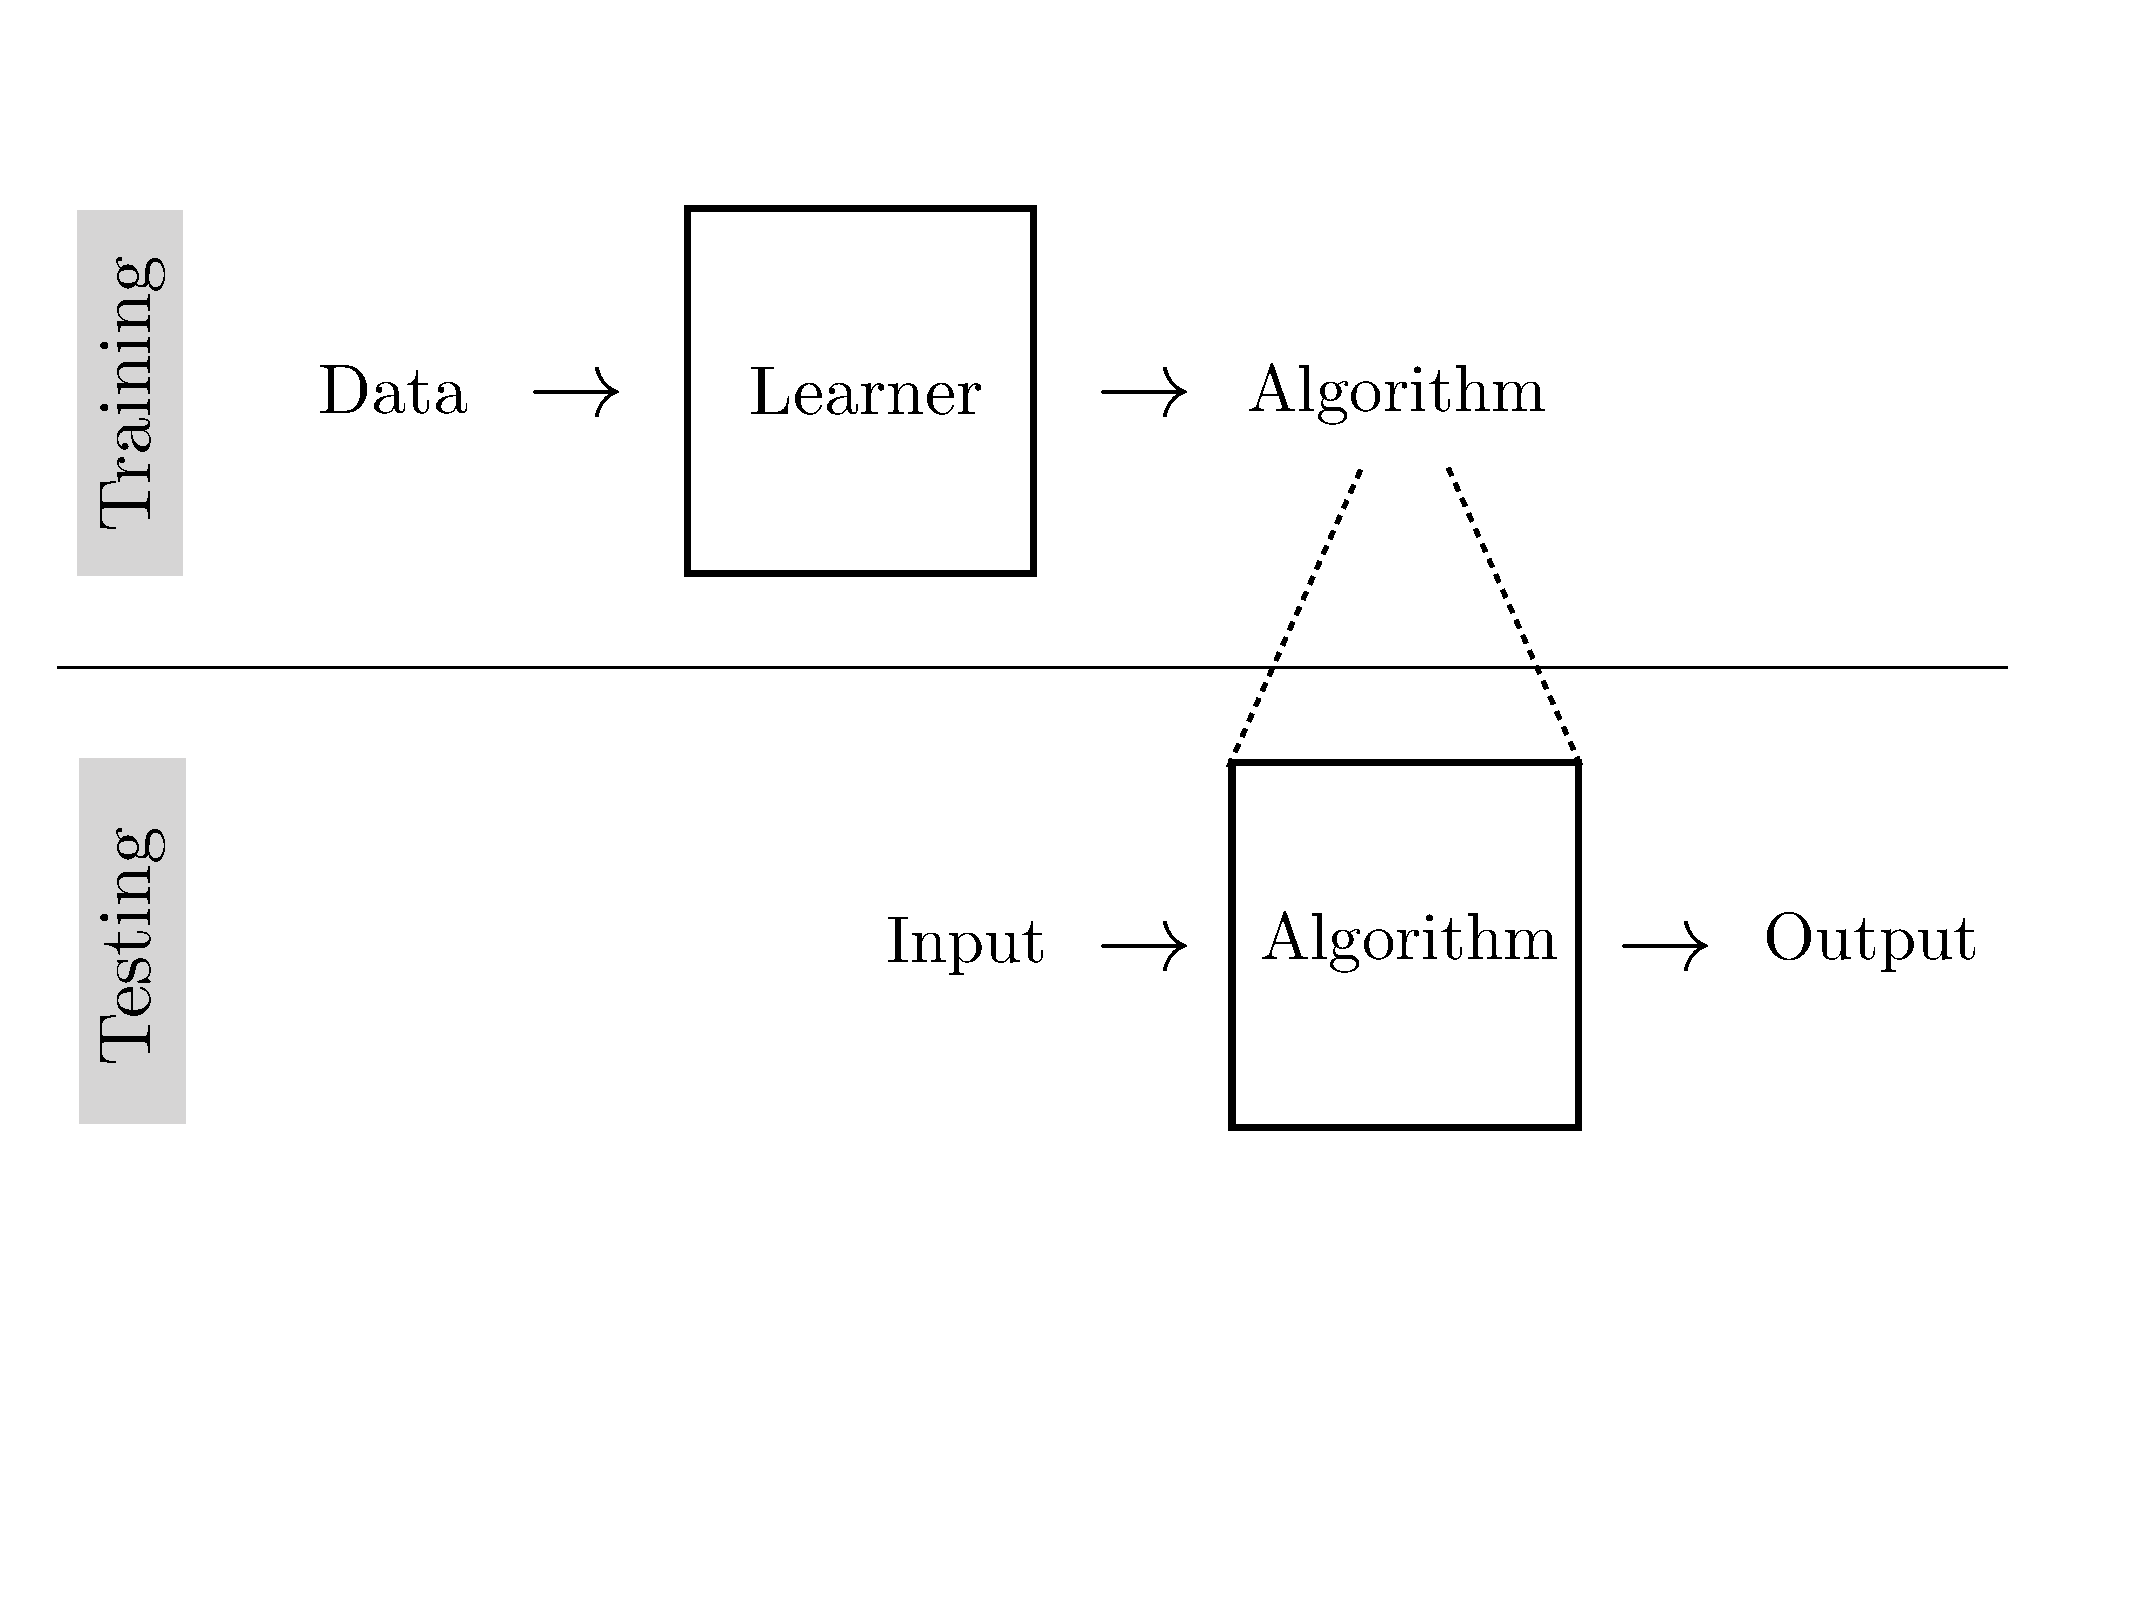
\includegraphics[width=0.75\linewidth]{./figures/intro_to_learning/learning_as_meta_algorithm.pdf}
    }
    \caption{Learning is an algorithm that outputs algorithms.}
    \label{fig:learning_as_meta_algorithm}
\end{figure}

Learning usually consists of two phases: the \index{Training phase}{\bf training} phase, where we search for an algorithm that performs well on past instances of the problem (training data), and the \index{Testing phase}{\bf testing} phase, where we deploy our learned algorithm to solve new instances of the problem.

%What exactly is an instance of a ``problem"? A common definition is a \{\texttt{question}, \texttt{answer}\} pair. Solving the problem consists of providing the \texttt{answer} to the \texttt{question}. From this perspective, a machine learning algorithm produces a set of rules that map \texttt{questions} to \texttt{answers}. A more general way to think of it is a machine learning algorithm produces a mapping from \texttt{inputs} to desirable \texttt{outputs}.

\section{Learning from Examples}
\marginnote{Learning from examples is also called \textbf{supervised learning}.}[-0.6cm]

%\marginnote{Learning from examples is sometimes called {\bf supervised learning}.}[-0.83cm]

Imagine you find an ancient mathematics text, with marvelous looking proofs, but there is a symbol you do not recognize, ``$\star$". You see it being used here and there in equations, and you note down examples of its behavior:
\begin{align}
    2 \star 3 &= 36\nonumber \\
    7 \star 1 &= 49\nonumber \\
    5 \star 2 &= 100\nonumber \\
    2 \star 2 &= 16\nonumber
\end{align}
What do you think $\star$ represents? What function is it computing? Do you have it? Let's test your answer: what is the value of $3 \star 5$? (The answer is in the figure below.)

It may not seem like it, but you just performed learning! You \emph{learned} what $\star$ does by looking at examples. In fact, \fig{\ref{fig:star_symbol_learning}} shows what you did:

\begin{figure}[h]
    \centerline{
    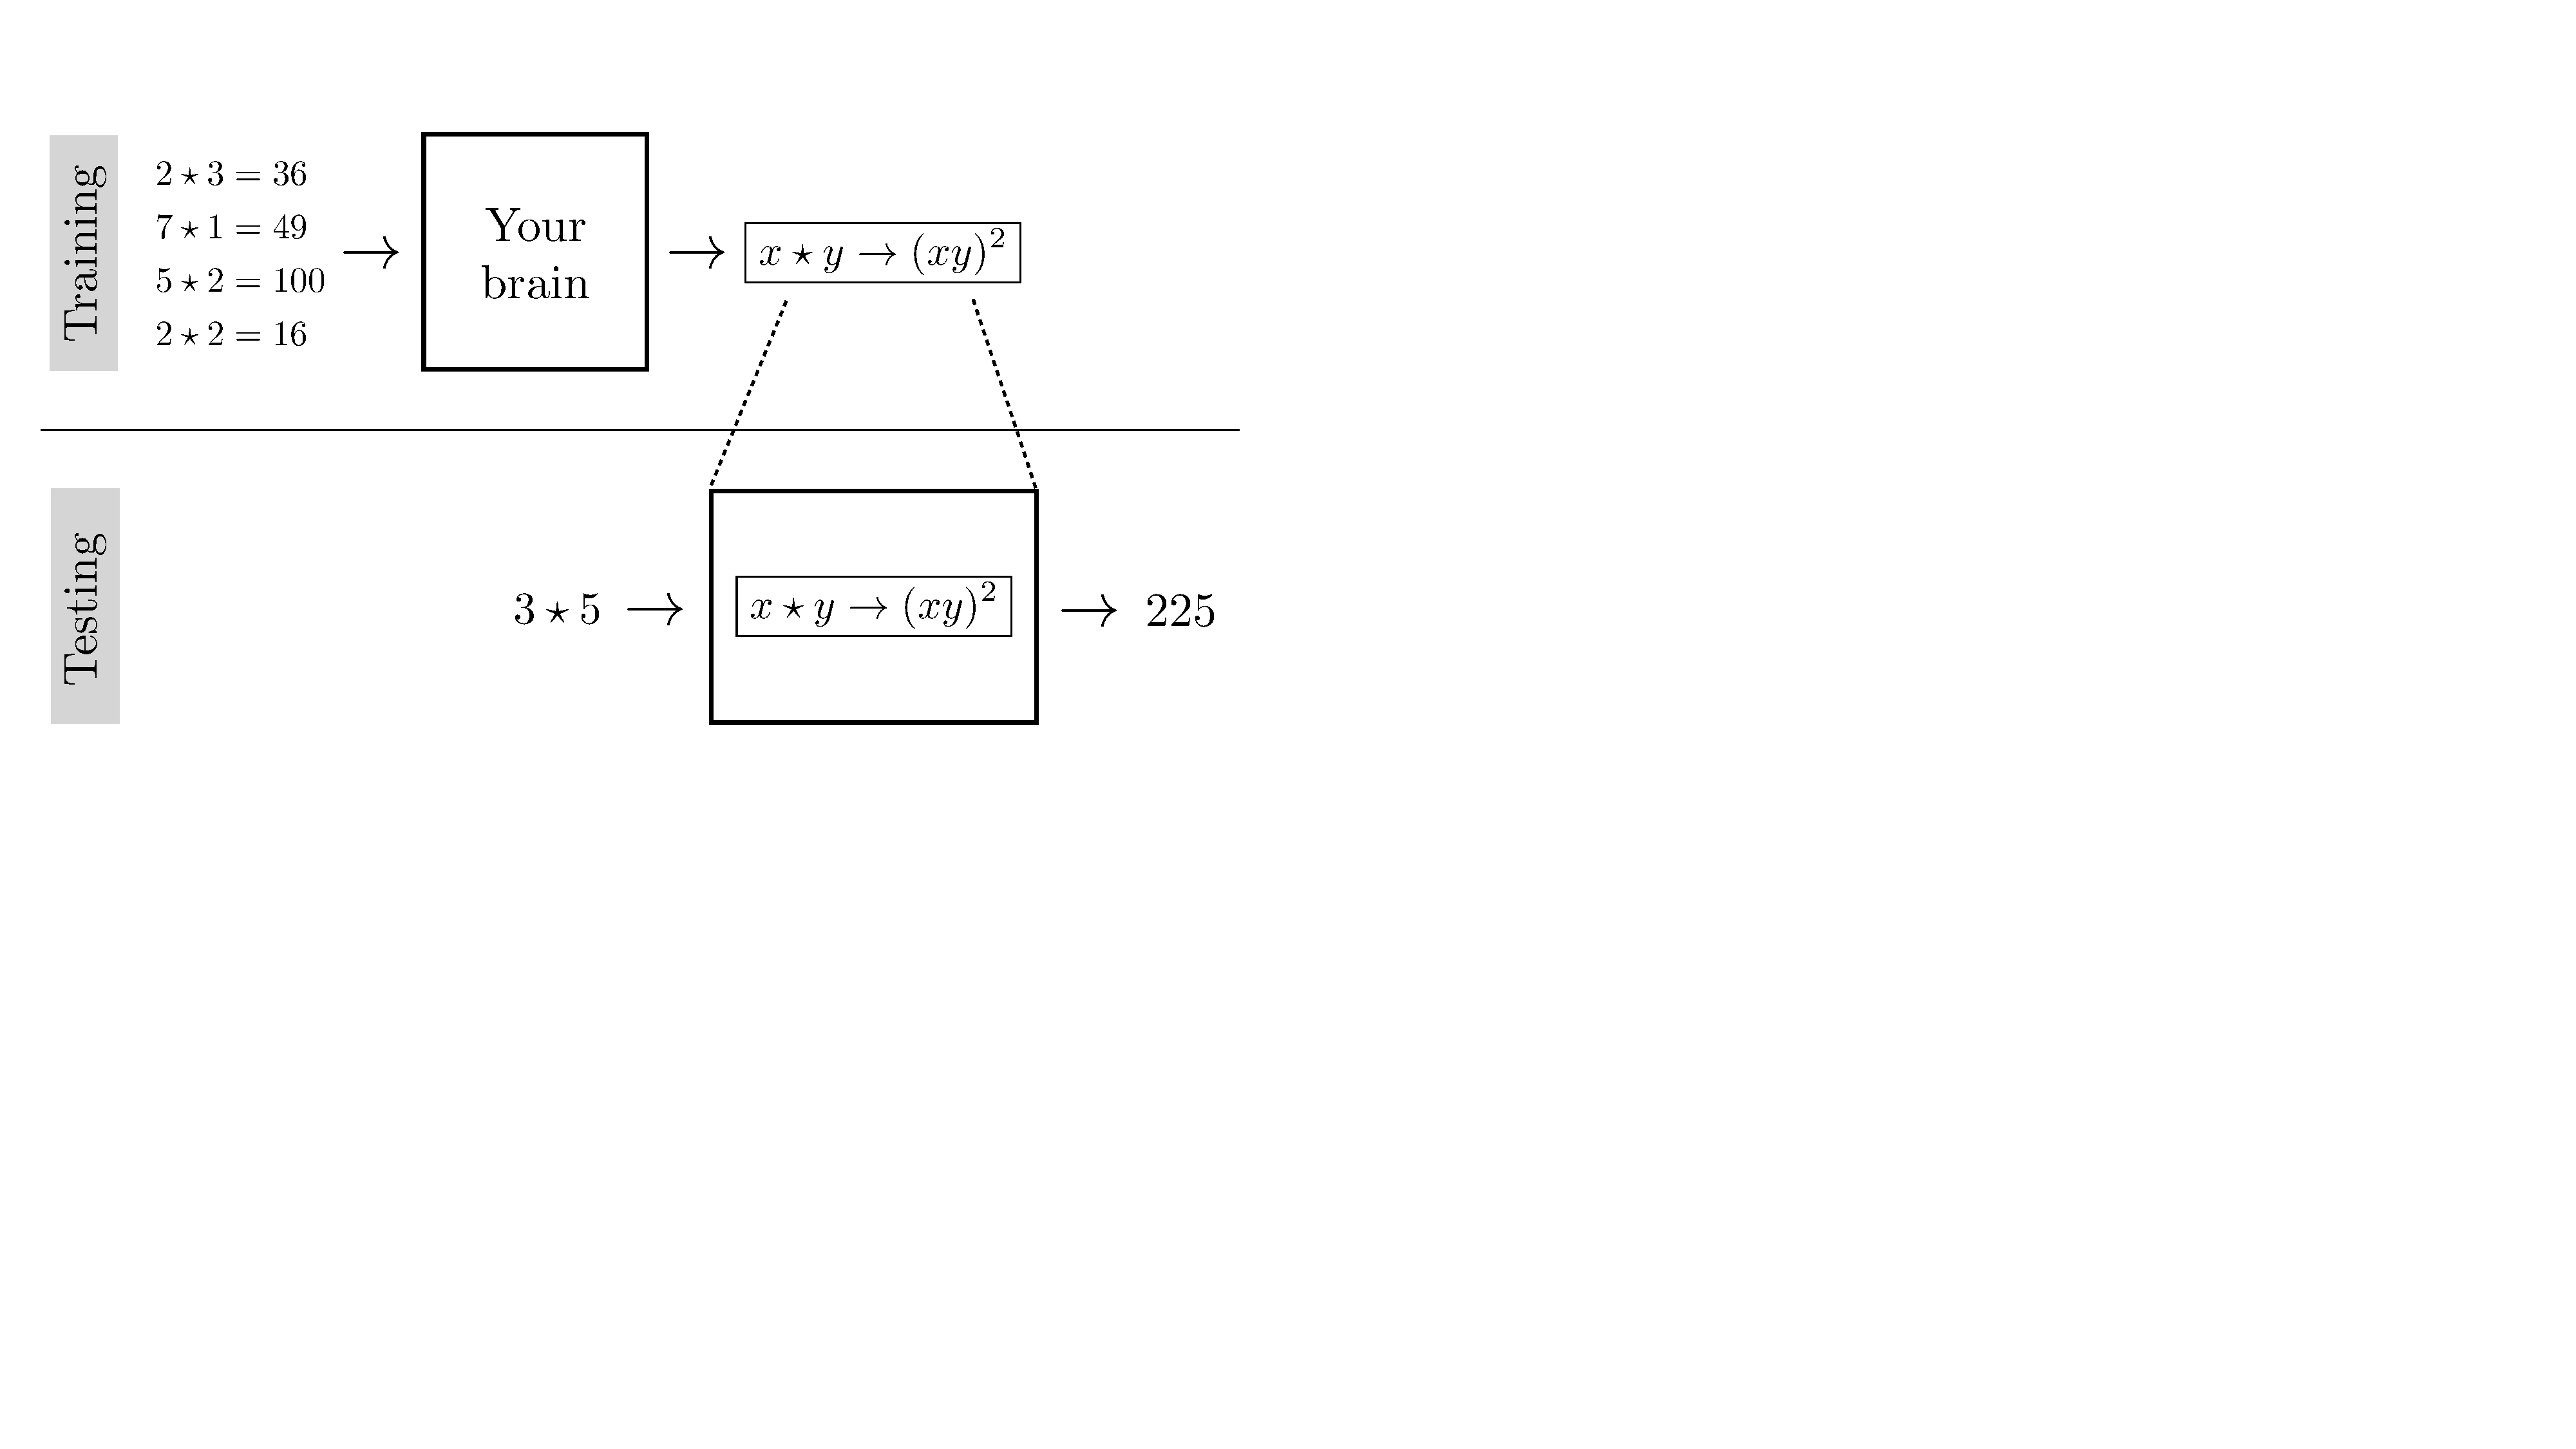
\includegraphics[width=0.75\linewidth]{./figures/intro_to_learning/star_symbol_learning.pdf}
    }
    \caption{How your brain may have solved the star problem.}
    \label{fig:star_symbol_learning}
\end{figure}

Nice job!

It turns out, we can learn almost anything from examples. 
Remember that we are learning an \emph{algorithm}, i.e., a computable mapping from inputs to outputs. A formal definition of \emph{example}, in this context, is an \{\texttt{input}, \texttt{output}\} pair. The examples you were given for $\star$ consisted of four such pairs:
\begin{align}
    &\{\texttt{input:} [2,3], \texttt{output:} 36\}\nonumber \\
    &\{\texttt{input:} [7,1], \texttt{output:} 49\}\nonumber \\
    &\{\texttt{input:} [5,2], \texttt{output:} 100\}\nonumber \\
    &\{\texttt{input:} [2,2], \texttt{output:}16\}\nonumber
\end{align}
This kind of learning, where you observe example input-output behavior and infer a functional mapping that explains this behavior, is called \index{Supervised learning}\textbf{supervised learning}. 

\marginnote{Another name for this kind of learning is {\bf fitting a model} to data.}[-1cm]

We were able to model the behavior of $\star$, on the examples we were given, with a simple algebraic equation. Let's try something rather more complicated. From the three examples in \fig{\ref{fig:intro_to_learning:inpainting_example}}, can you figure out what the operator $F$ does?

\begin{figure}[h]
    \centerline{
    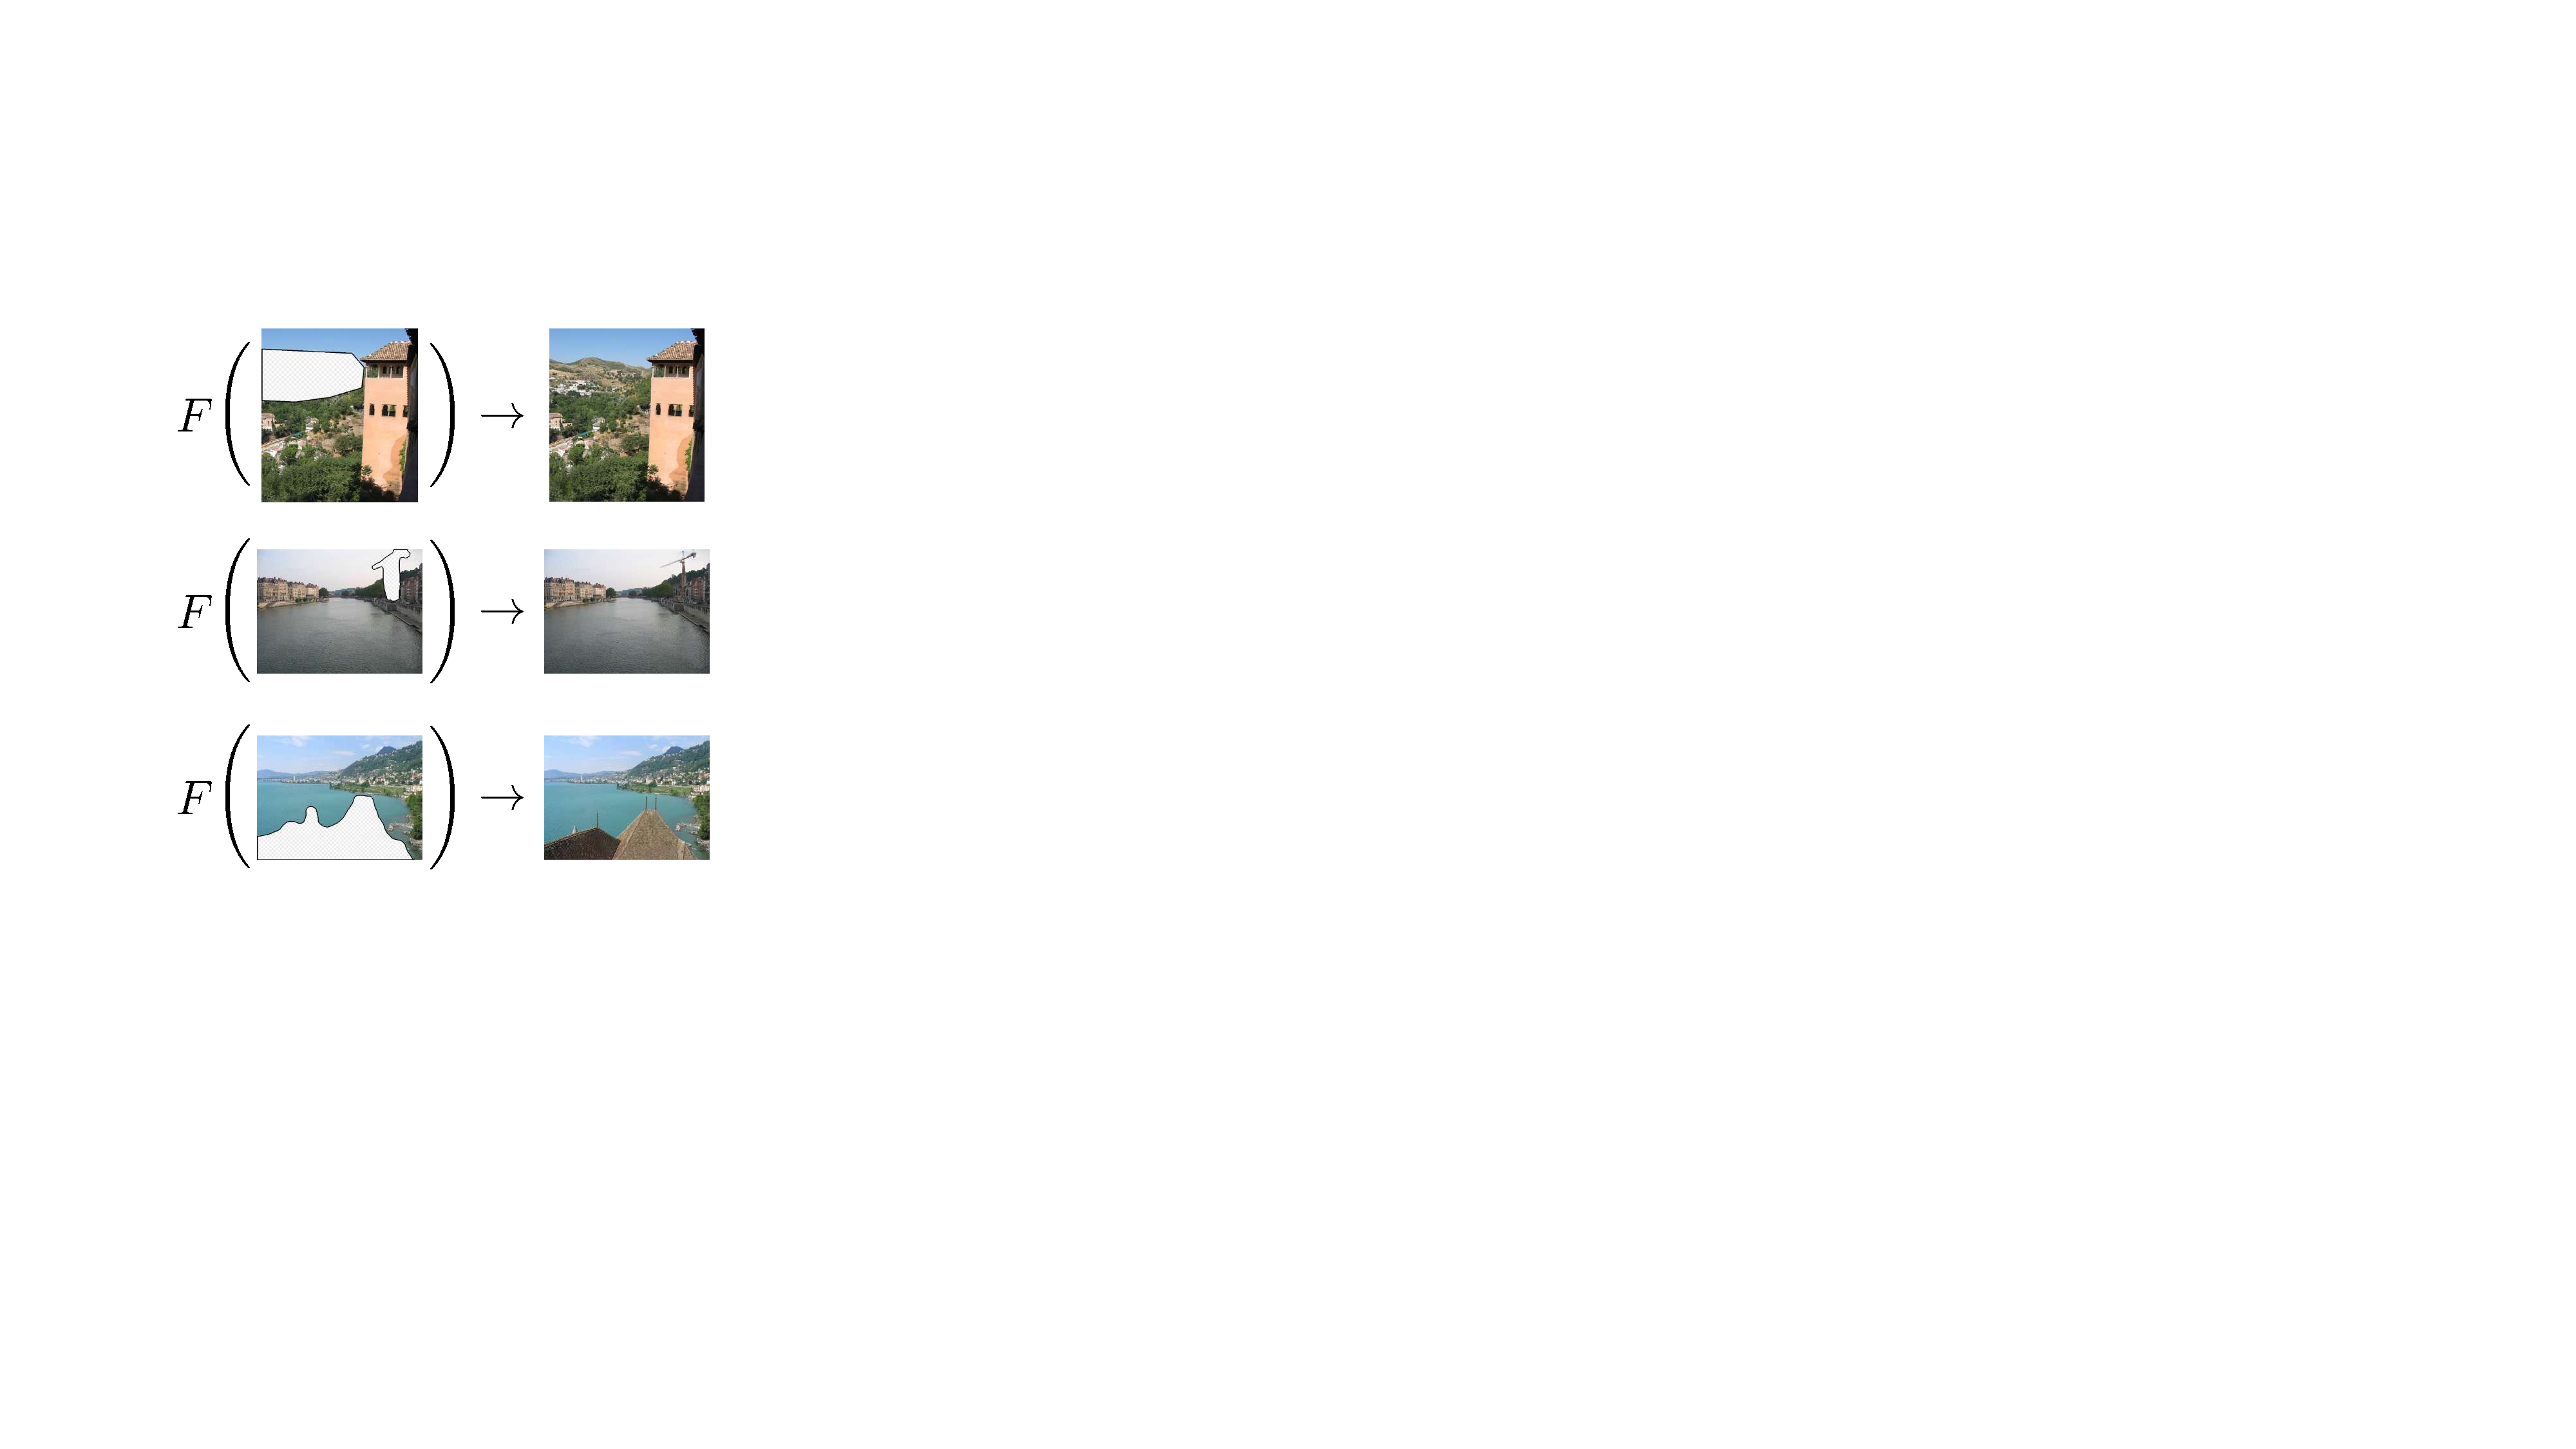
\includegraphics[width=0.4\linewidth]{./figures/intro_to_learning/inpainting_example.pdf}
    }
    \caption{A complicated function that could be learned from examples. This example is from \cite{hays2007scene}. \reviewcomment{Get permission}}
    \label{fig:intro_to_learning:inpainting_example}
\end{figure}

You probably came up with something like ``it fills in the missing pixels.'' That's exactly right, but it's sweeping a lot of details under the rug. Remember, we want to learn an \emph{algorithm}, a procedure that is completely unambiguous. How exactly does $F$ fill in the missing pixels? 

It's hard to say in words. We may need a very complex algorithm to specify the answer, an algorithm so complex that we could never hope to write it out by hand. This is the point of machine learning. The machine writes the algorithm for us, but it can only do so if we give it many examples, not just these three.

\marginnote{Some things are not learnable from examples, such as noncomputable functions. An example of a noncomputable function is a function that takes as input a program and outputs a 1 if the program will eventually finish running, and a 0 if it will run forever. It is noncomputable because there is no algorithm that can solve this task in finite time. However, it might be possible to learn a good approximation to it.}[-.7in] 

\section{Learning without Examples}
%\marginnote{Methods for learning without examples include \textbf{unsupervised learning} and \textbf{reinforcement learning}.}

Even without examples, we can still learn. Instead of matching input-output examples, we can try to come up with an algorithm that optimizes for desirable \emph{properties} of the input-output mapping. This class of learners includes \index{Unsupervised learning}{\bf unsupervised learning} and \index{Reinforcement learning}{\bf reinforcement learning}. 

%In both of these frameworks, we are given an \textbf{objective function} that scores the quality of the learned function's output.

In unsupervised learning, we are given examples of \textit{input data} $\{x^{(i)}\}^N_{i=1}$ but we are not told the target outputs $\{y^{(i)}\}^N_{i=1}$. Instead the learner has to come up with a model or representation of the input data that has useful properties, as measured by some \textbf{objective function}. The objective could be, for example, to compress the data into a lower dimensional format that still preserves all information about the inputs. We will encounter this kind of learning in \partref{\ref{part:generative_models_and_representation_learning}} of this book, on representation learning and generative modeling.

In reinforcement learning, we suppose that we are given a 
\index{Reward function}{\bf reward function} that explicitly measures the quality of the learned function's output. To be precise, a reward function is a mapping from outputs to scores: $r: \mathcal{Y} \rightarrow \mathbb{R}$. The learner tries to come up with a function that maximizes rewards. This book will not cover reinforcement learning in detail, but this kind of learning is becoming an important part of computer vision, especially in the context of vision for robots. We direct the interested reader to \cite{sutton2018reinforcement} to learn more.%Reinforcement learning also usually deals with the setting where the learned function gets to pick which training datapoints to observe next, rather than being provided them passively. An example is an agent that chooses which actions to take as it navigates a room, and this choice of action determines what data (view of the world) the agent will next observe. This dependence of data on learned function is one of the main reasons reinforcement learning is hard.
\marginnote{At first glance unsupervised learning and reinforcement learning look similar: both maximize a function that scores desirable properties of the input-output mapping. The big difference is that unsupervised learning has access to \textit{training data} whereas reinforcement learning usually does not; instead the reinforcement learner has to collect its own training data.}[-5cm]


\section{Key Ingredients}
\label{sec:intro_to_learning:key_ingredients}

A learning algorithm consists of three key ingredients:
\begin{enumerate}
    \item \index{Objective function}{\bf Objective}: What does it mean for the learner to succeed, or, at least, to perform well? 
    \item \index{Hypothesis space}{\bf Hypothesis space}: What is the set of possible mappings from inputs to outputs that we will we search over?
    \item \index{Optimizer}{\bf Optimizer}: \emph{How}, exactly, do we search the hypothesis space for a specific mapping that maximizes the objective?
\end{enumerate}
%\marginnote{These three ingredients will help organize our thinking in this book, but they are not meant to be comprehensive. In particular, we can drill down into any one of these categories and find interesting additional choices. For example, after choosing a hypothesis space, the next critical decision is how to \textit{parameterize} the hypothesis space. We discuss this choice in Section XX.}

These three ingredients, when applied to large amounts of data, and run on sufficient hardware (referred to as {\bf compute}) can do amazing things. We will focus on the learning algorithms in this chapter, but often the data and compute turn out to be more important.

\begin{center}
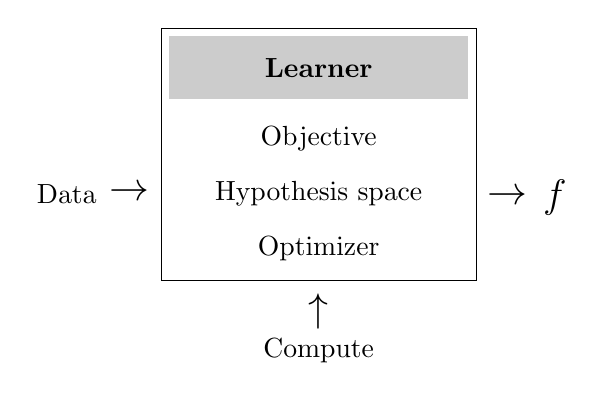
\begin{tikzpicture}
    \draw (0,0) rectangle (4,3.2); % outer box
    \fill[black!20] (0.1,2.3) rectangle (3.9,3.1); % gray box
    \node[] at (2,2.7) {{\bf Learner}};
    \node[] at (2,1.8) {Objective};
    \node[] at (2,1.1) {Hypothesis space};
    \node[] at (2,0.4) {Optimizer};
    \node[] at (-1.2,1.1) {Data};
    \node[] at (-0.4,1.1) {{\Large  $ \rightarrow$}};
    \node[] at (5,1.05) {{\Large $f$}};
    \node[] at (4.4,1.05) {{\Large  $ \rightarrow$}};
    \node[] at (2,-0.4) {{\Large  $ \uparrow$}};
    \node[] at (2,-0.9) {Compute};
\label{fig:ingredients}
\end{tikzpicture}
\end{center}

% \begin{figure}[h]
%     \centering
%     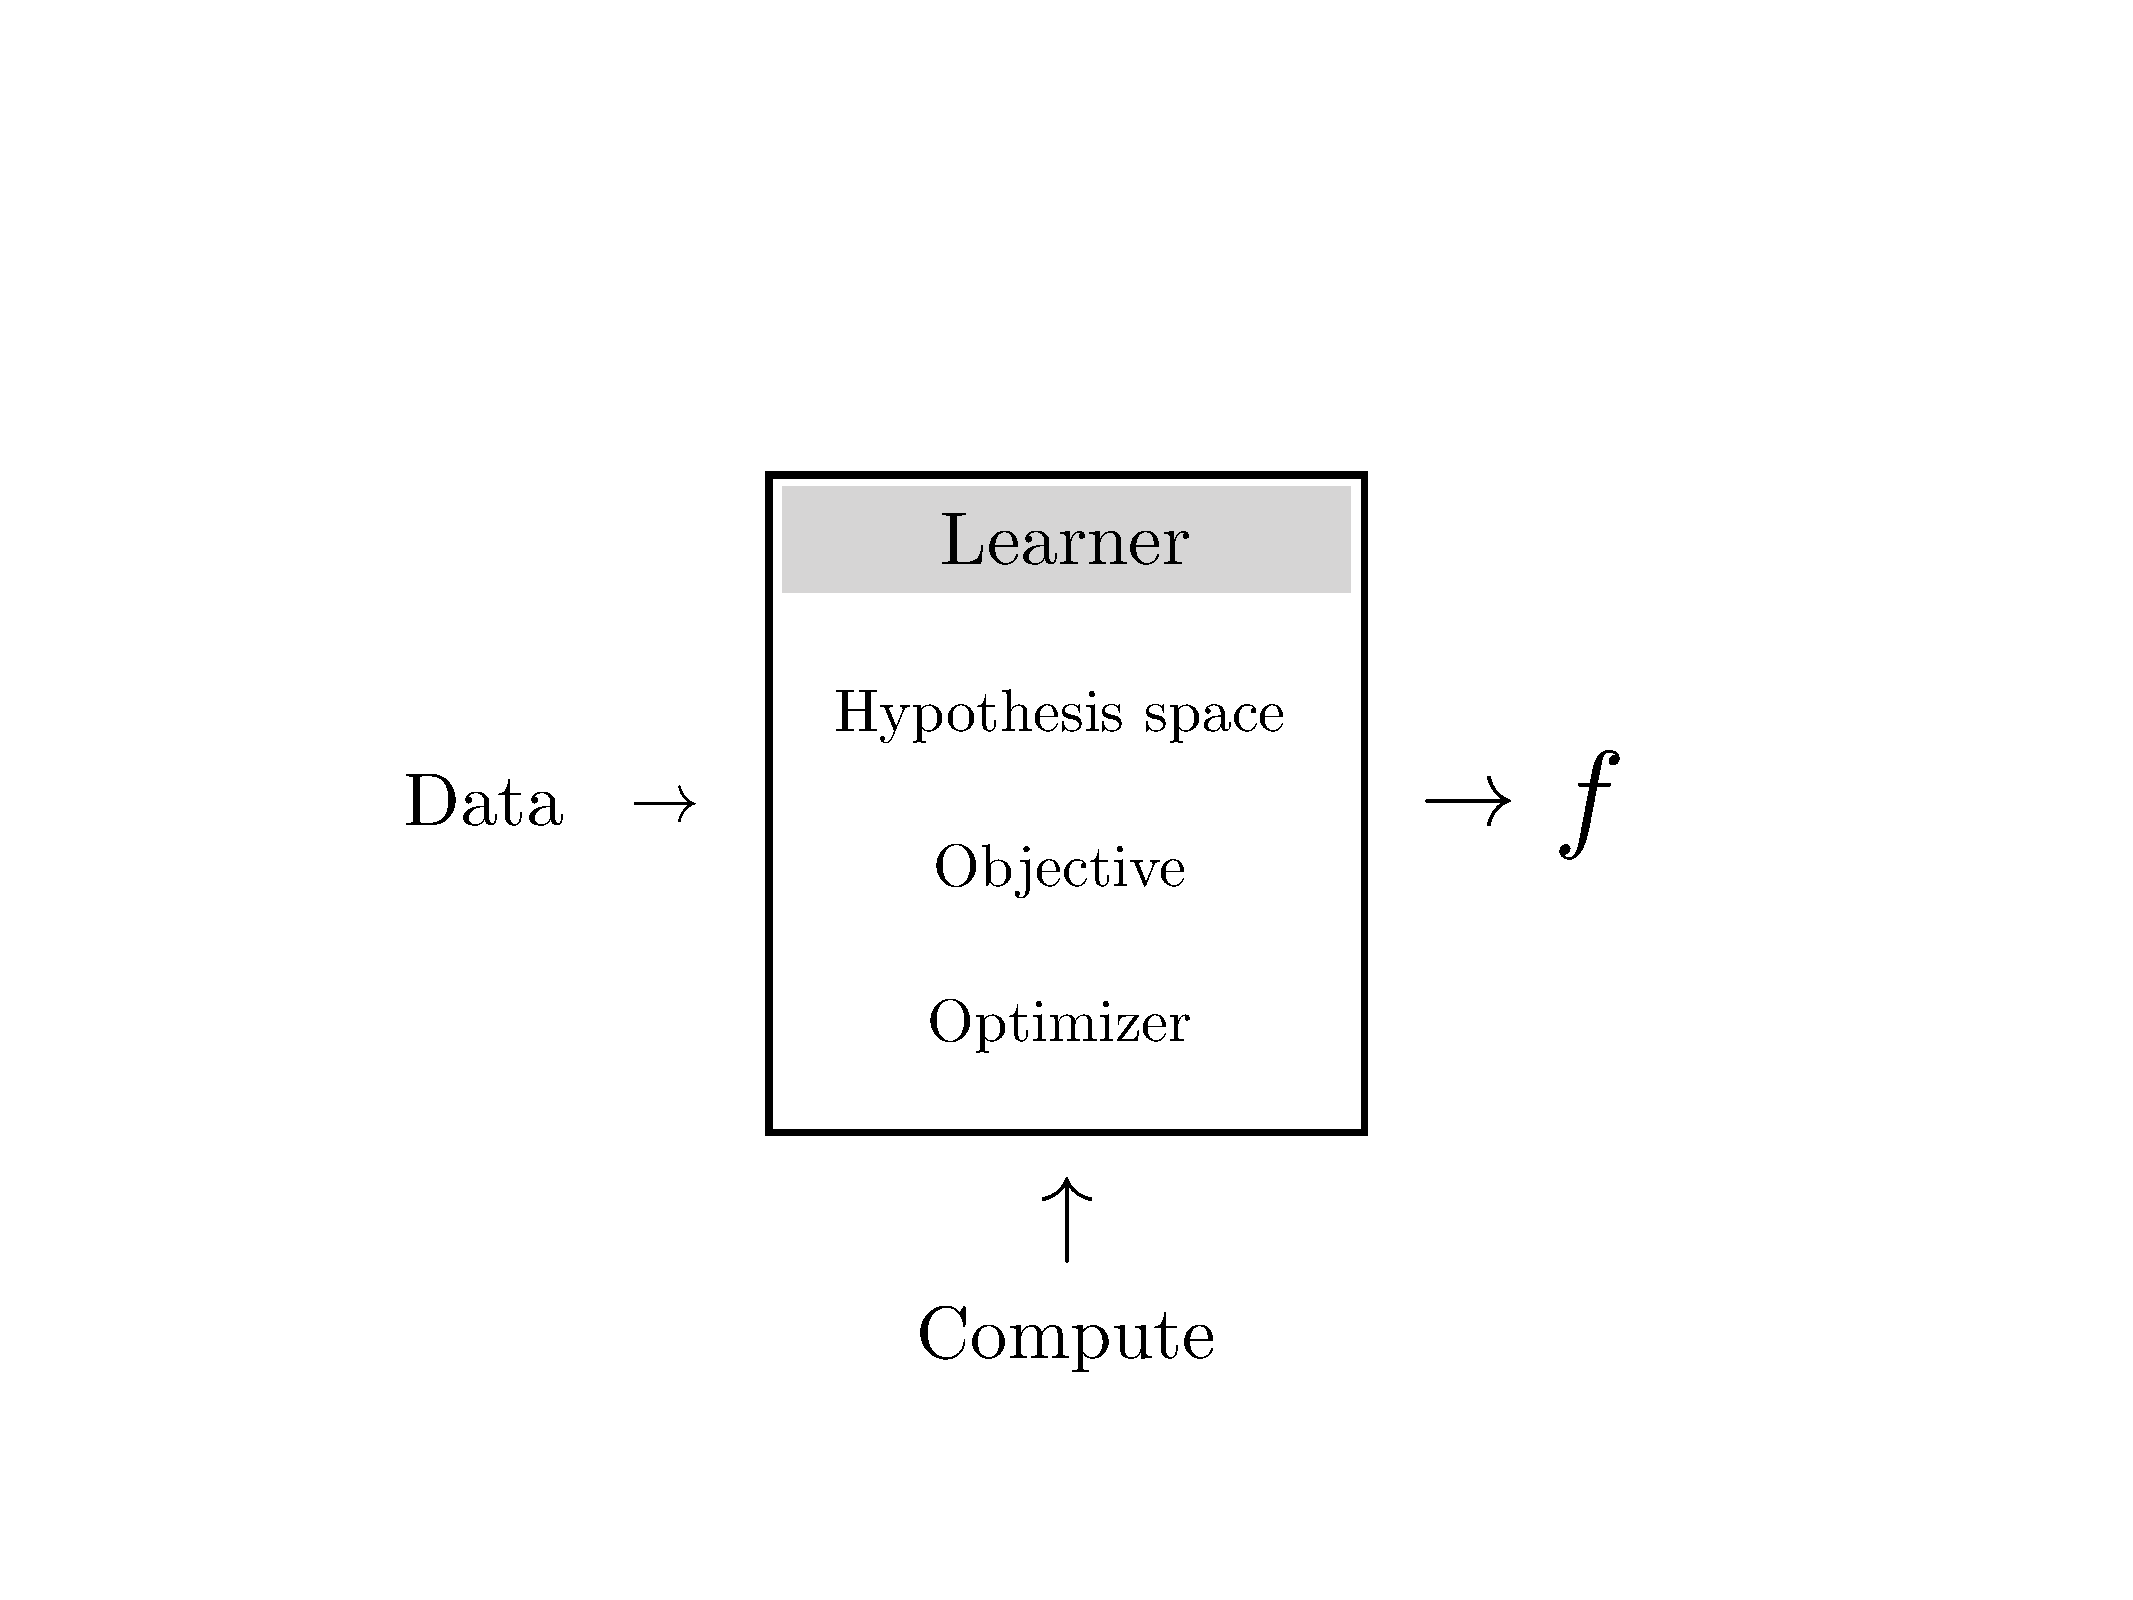
\includegraphics[width=0.5\linewidth]{./figures/intro_to_learning/ingredients.pdf}
%     \label{fig:ingredients}
% \end{figure}

A learner outputs an algorithm, $f: \mathcal{X} \rightarrow \mathcal{Y}$, which maps inputs, $\mathbf{x} \in \mathcal{X}$, to outputs, $\mathbf{y} \in \mathcal{Y}$. Commonly, $f$ is referred to as the \index{Learned function}\textbf{learned function}. The objective that the learner optimizes is typically a function that scores model outputs, $\mathcal{L}: \mathcal{Y} \rightarrow \mathbb{R}$, or compares model outputs to target answers, $\mathcal{L}: \mathcal{Y} \times \mathcal{Y} \rightarrow \mathbb{R}$. We will interchangeably call this $\mathcal{L}$ either the \textbf{objective function}, the \index{Loss function}\textbf{loss function}, or the \textbf{loss}. A loss almost always refers to an objective we seek to \textit{minimize}, whereas an objective function can be used to describe objectives we seek to minimize as well as those we seek to maximize.

\subsection{Importance of Parameterization} The hypothesis space can be described by a set $\mathcal{F}$ of all the possible functions under consideration by the learner. For example, one hypothesis space might be ``all mappings from $\mathbb{R}^2 \rightarrow \mathbb{R}$'' and another could be ``all functions $\mathbb{R} \times \mathbb{R} \rightarrow \mathbb{R}_{\geq 0}$ that satisfy the conditions of being a distance metric.'' Commonly, however, we will not just specify the hypothesis space, but also how we parameterize the space. For example, we may say that our \textit{parameterized} hypothesis space is $y = \theta_1 x + \theta_0$, where $\theta_0$ and $\theta_1$ are the parameters. This example corresponds to the space of affine functions from $\mathbb{R} \rightarrow \mathbb{R}$, but this is not the only way to parameterize that space. Another choice could be $y = \theta_2\theta_1 x + \theta_0$, with parameters $\theta_0$, $\theta_1$, and $\theta_2$. These two choices parameterize \textit{exactly the same space}, that is, any affine functions can be represented by either parameterization and both parameterizations can only represent affine functions. However, these two parameterizations are not equivalent, because optimizers and objectives may treat different parameterizations differently. Because of this, to fully define a learning algorithm, it is important to specify how the hypothesis space is parameterized.\marginnote{\index{Overparameterization}\textbf{Overparameterized} models, where you use more parameters than the minimum necessary to fit the data, are especially important in modern computer vision; most neural networks (\chap{\ref{chapter:neural_nets}}) are overparameterized.}[-3.4cm]
%\marginnote{Recall that a metric function is a very constrained class of functions; metrics must satisfy the triangle inequality, symmetry, nonnegativity, and ``identity of indiscernibles."}
%\marginnote{The role of parameterization can be subtle but should not be overlooked. Historically ... }

\section{Empirical Risk Minimization: A Formalization of Learning from Examples}

The three ingredients from the last section can be formalized using the framework of \index{Empirical risk minimization}{\bf empirical risk minimization} ({\bf ERM}). This framework applies specifically to the supervised setting where we are learning a function that predicts $\mathbf{y}$ from $\mathbf{x}$ given many training examples $\{\mathbf{x}^{(i)},\mathbf{y}^{(i)}\}^N_{i=1}$. The idea is to minimize the average error (i.e., risk) we incur over all the training data (i.e., empirical distribution). The ERM problem is stated as follows:
\begin{align}
    \argmin_{f \in \mathcal{F}} \frac{1}{N} \sum_{i=1}^N \mathcal{L}(f(\mathbf{x}^{(i)}),\mathbf{y}^{(i)}) \quad\triangleleft\quad \text{ERM}
\end{align}
Here, $\mathcal{F}$ is the hypothesis space, $\mathcal{L}$ is the loss function, and $\{\mathbf{x}^{(i)}, \mathbf{y}^{(i)}\}_{i=1}^N$ is the training data (example \{\texttt{input}, \texttt{output}\} pairs), and $f$ is the learned function.

\section{Learning as Probabilistic Inference}
Depending on the loss function, there is often an interpretation of ERM as doing maximum likelihood probabilistic inference. In this interpretation, we are trying to infer the hypothesis $f$ that assigns the highest probability to the data. For a model that predicts $\mathbf{y}$ given $\mathbf{x}$, the max likelihood $f$ is:
\begin{align}
    \argmax_f p\big(\{\mathbf{y}^{(i)}\}_{i=1}^N \given \{\mathbf{x}^{(i)}\}_{i=1}^N, f\big) \quad\quad \triangleleft \quad\text{Max likelihood learning}
\end{align}
The term $p\big(\{\mathbf{y}^{(i)}\}_{i=1}^N \given \{\mathbf{x}^{(i)}\}_{i=1}^N, f\big)$ is called the \index{Likelihood}\textbf{likelihood} of the $\mathbf{y}$ values given the model $f$ and the observed $\mathbf{x}$ values, and maximizing this quantity is called \index{Maximum likelihood learning}\textbf{maximum likelihood learning}.\marginnote{To fully specify this model, we have to define the form of this conditional distribution. One common choice is that the prediction errors, $(\mathbf{y} - f(\mathbf{x}))$, are Gaussian distributed, which leads to the least-squares objective (\sect{\ref{sec:intro_to_learning:least_squares}}).}[-0.4cm]

In later chapters we will see that \textbf{priors} $p(f)$ can also be used for inferring the most probable hypothesis. When a prior is used in conjunction with a likelihood function, we arrive at \index{Maximum a posteriori learning}\textbf{maximum a posteriori learning} (\textbf{MAP learning}), which infers the most probable hypothesis given the training data:
\begin{align}
    &\argmax_f p\big(f \given \{\mathbf{x}^{(i)}, \mathbf{y}^{(i)}\}_{i=1}^N\big) \quad\quad \triangleleft \quad \text{MAP learning}\\
    & = \argmax_f p\big(\{\mathbf{y}^{(i)}\}_{i=1}^N \given \{\mathbf{x}^{(i)}\}_{i=1}^N, f\big)p\big(f\big) \quad\quad \triangleleft \quad \text{by Bayes' rule}
\end{align}


%For example, the least squares regression example we saw above can be interpreted as finding the maximum likelihood estimate of the parameters $\theta$ given the assumption that there truly exists a linear relationship between $x$ and $y$ but that training observations of $y$ are corrupted by Gaussian noise (and we assume that training datapoints are independent and identically distributed, i.e. {\bf iid}).





\section{Case Studies}
The next three sections cover several case studies of particular learning problems. Examples 1 and 3 showcase the two most common workhorses of machine learning: regression and classification. Example 2, Python program induction, demonstrates that the paradigms in this chapter are not limited to simple systems but can actually apply to very general and sophisticated models.

\subsection{Example 1: Linear Least-Squares Regression}\label{sec:intro_to_learning:least_squares}
One of the simplest learning problems is known as \index{Linear least-squares regression}\textbf{linear least-squares regression}. In this setting, we aim to model the relationship between two variables, $x$ and $y$, with a line. 

As a concrete example, let's imagine $x$ represents the temperature outside, and $y$ represents the number people at the beach. As before, we train (i.e., fit) our model on many observed examples of \{\texttt{temperature outside}, \texttt{number of people at the beach}\} pairs, denoted as $\{x^{(i)},y^{(i)}\}_{i=1}^N$. At test time, this model can be applied to predict the $y$ value of a new query $x'$, as shown in \fig{\ref{fig:intro_to_learning:ols_train_test}}.

\begin{figure}[h]
    \centerline{
    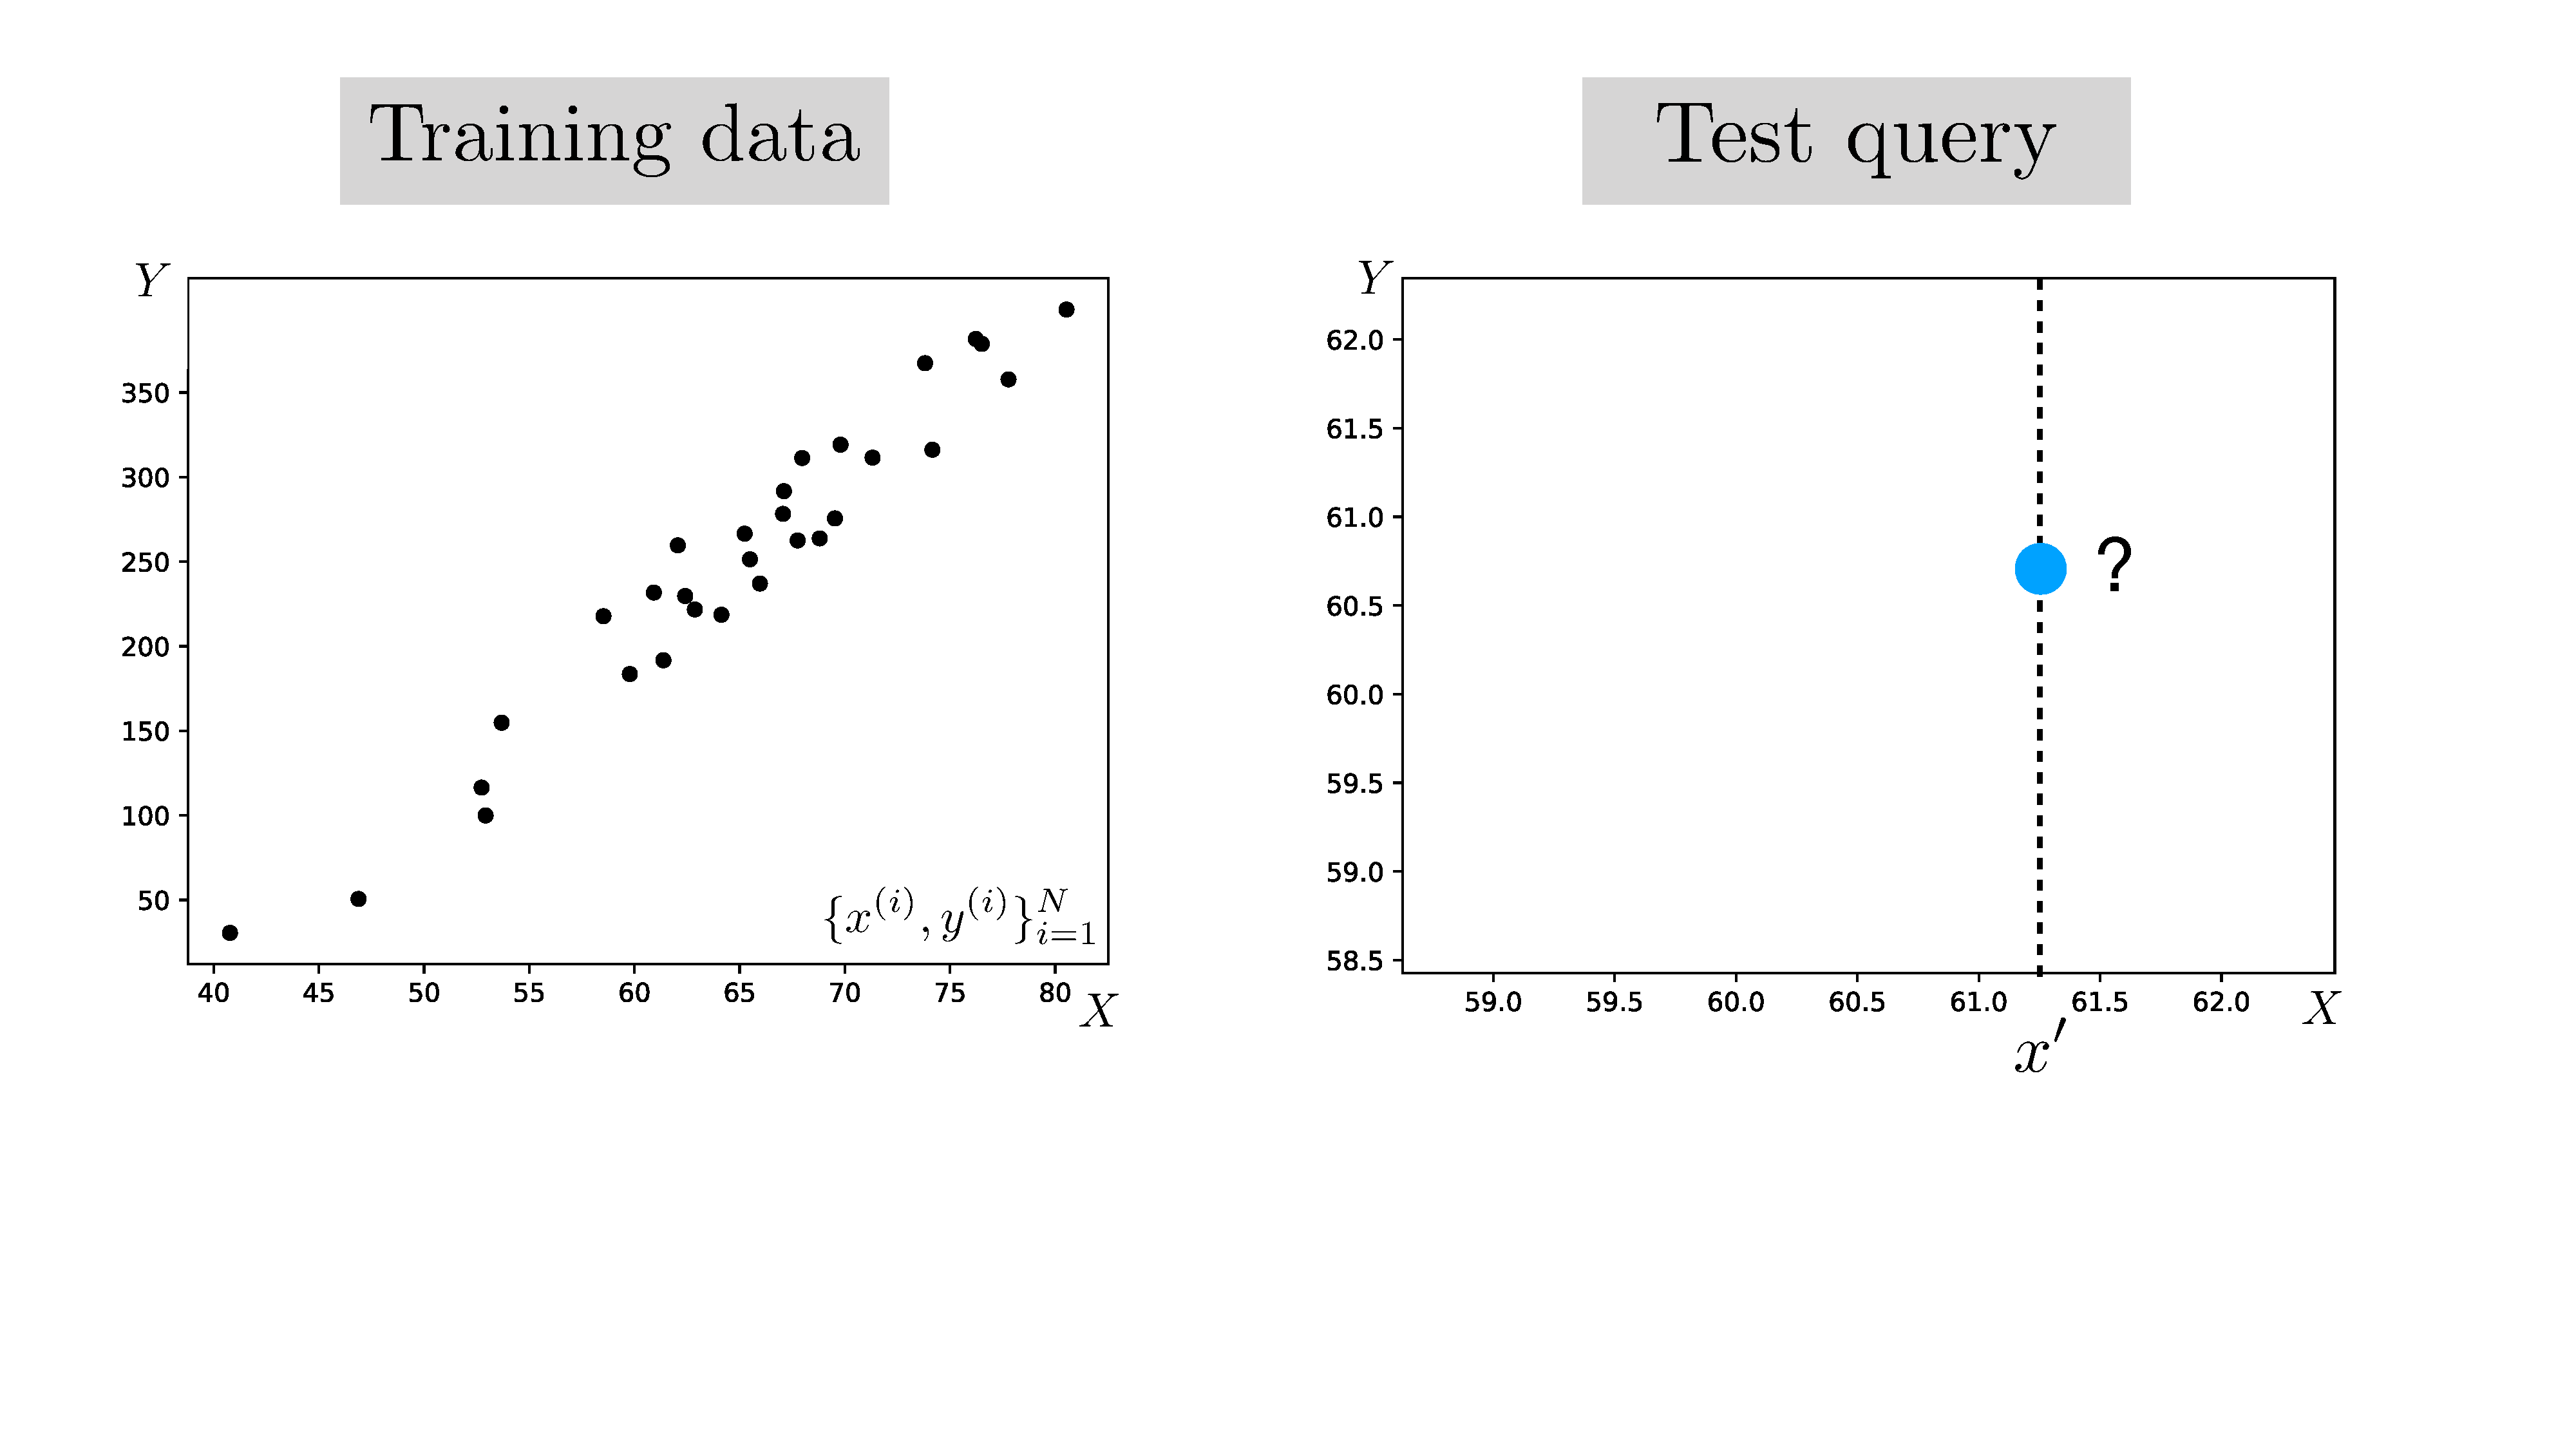
\includegraphics[width=0.7\linewidth]{./figures/intro_to_learning/ols_train_test.pdf}
    }
    \caption{The goal of learning is to use the training data to predict the $y$ value of the test query. In our example we find that for every 1 degree increase in temperature, we can expect $\sim 10$ more people to go to the beach.}
    \label{fig:intro_to_learning:ols_train_test}
\end{figure}

Our \emph{hypothesis space} is linear functions, that is, the relationship between $x$ and our predictions $\hat{y}$ of $y$ has the form $\hat{y} = f_{\theta}(x) = \theta_1 x + \theta_0$. This hypothesis space is parameterized by a two scalars, $\theta_0, \theta_1 \in \mathbb{R}$, the intercept and slope of the line. In this book, we will use $\theta$ in general to refer to any parameters that are being learned. In this case we have $\theta = [\theta_0, \theta_1]$. Learning consists of finding the value of these parameters that maximizes the objective.

Our \emph{objective} is that predictions should be near ground truth targets in a least-squares sense, that is, $(\hat{y}^{(i)} - y^{(i)})^2$ should be small for all training examples $\{x^{(i)}, y^{(i)}\}_{i=1}^N$. We call this objective the $L_2$ loss:
\begin{align}
    J(\theta) &= \sum_i \mathcal{L}(\hat{y}^{(i)}, y^{(i)})\\
    &\quad \mathcal{L}(\hat{y}, y) = (\hat{y} - y)^2 \quad\quad \triangleleft \quad L_2 \text{ loss}
\end{align}
\marginnote{We will use $J(\theta)$ to denote the total objective, over all training datapoints, as a function of the parameters; we will use $\mathcal{L}$ to denote the loss per datapoint. That is, $J(\theta) = \sum_{i=1}^N \mathcal{L}(f_{\theta}(x^{(i)}), y^{(i)})$.}[-1.5cm]%Some texts refer to $J$, rather than $\mathcal{L}$, as the ``loss function", but we will reserve the distinct term ``total cost" for $J$ and ``loss" for $\mathcal{L}$.}

%$\mathcal{L}(\hat{y},y) = (\hat{y} - y)^2$ is referred to as the {\bf loss function}, which is defined as the negative of the objective.
%\marginnote{Minimizing the {\bf loss} is equivalent to maximizing the objective.}[-0.0cm]

The full learning problem is as follows:
\begin{align}
    \theta^* = \argmin_{\theta} \sum_{i=1}^N (\theta_1 x^{(i)} + \theta_0 - y^{(i)})^2.
\end{align}
We can choose any number of optimizers to solve this problem. A first idea might be ``try a bunch of random values for $\theta$ and return the one that maximizes the objective.'' In fact, this simple approach works, it just can be rather slow since we are searching for good solutions blind. A better idea can be to exploit \textit{structure} in the search problem. For the linear least-squares problem, the tools of calculus give us clean mathematical structure that makes solving the optimization problem easy, as we show next.

From calculus, we know that at any maxima or minima of a function, $J(\theta)$, with respect to a variable $\theta$, the derivative $\frac{\partial{J(\theta)}}{\partial{\theta}} = 0$. We are trying to find the minimum of the objective $J(\theta)$:
\begin{align}
    J(\theta) = \sum_{i=1}^N (\theta_1 x^{(i)} + \theta_0 - y^{(i)})^2.
\end{align}
This function can be rewritten as
\begin{align}
    J(\theta) = (\mathbf{y} - \mathbf{X}\theta)^\transpose(\mathbf{y} - \mathbf{X}\theta)
\end{align}
with
\begin{align}
\mathbf{X} = 
 \begin{bmatrix}
    1 & x^{(1)}  \\
    1 & x^{(2)} \\
    \vdots & \vdots \\
    1 & x^{(N)}
\end{bmatrix}
\quad
\mathbf{y} = 
 \begin{bmatrix}
    y^{(1)}  \\
    y^{(2)} \\
    \vdots \\
    y^{(N)}
\end{bmatrix}
\quad
\theta = 
 \begin{bmatrix}
    \theta_0 \\
    \theta_1
\end{bmatrix}.
\end{align}

The $J$ is a quadratic form, which has a single global minimum where the derivative is zero, and no other points where the derivative is zero. Therefore, we can solve for the $\theta^*$ that minimizes $J$ by finding the point where the derivative is zero. The derivative is:
\begin{align}
    \frac{\partial J(\theta)}{\partial \theta} =  2(\mathbf{X}^\transpose \mathbf{X} \theta - \mathbf{X}^\transpose \mathbf{y}).
\end{align}
We set this derivative to zero and solve for $\theta^*$:
\begin{align}
    2(\mathbf{X}^\transpose \mathbf{X} \theta^* - \mathbf{X}^\transpose \mathbf{y}) &= 0\\
\mathbf{X}^\transpose \mathbf{X} \theta^* &= \mathbf{X}^\transpose \mathbf{y}\\
\theta^* &= (\mathbf{X}^\transpose\mathbf{X})^{-1}\mathbf{X}^\transpose\mathbf{y}.
\end{align}

The $\theta^*$ defines the best fitting line to our data, and this line can be used to predict the $y$ value of future observations of $x$ (\fig{\ref{fig:intro_to_learning:ols_fit}}).

\begin{figure}[h]
    \centerline{
    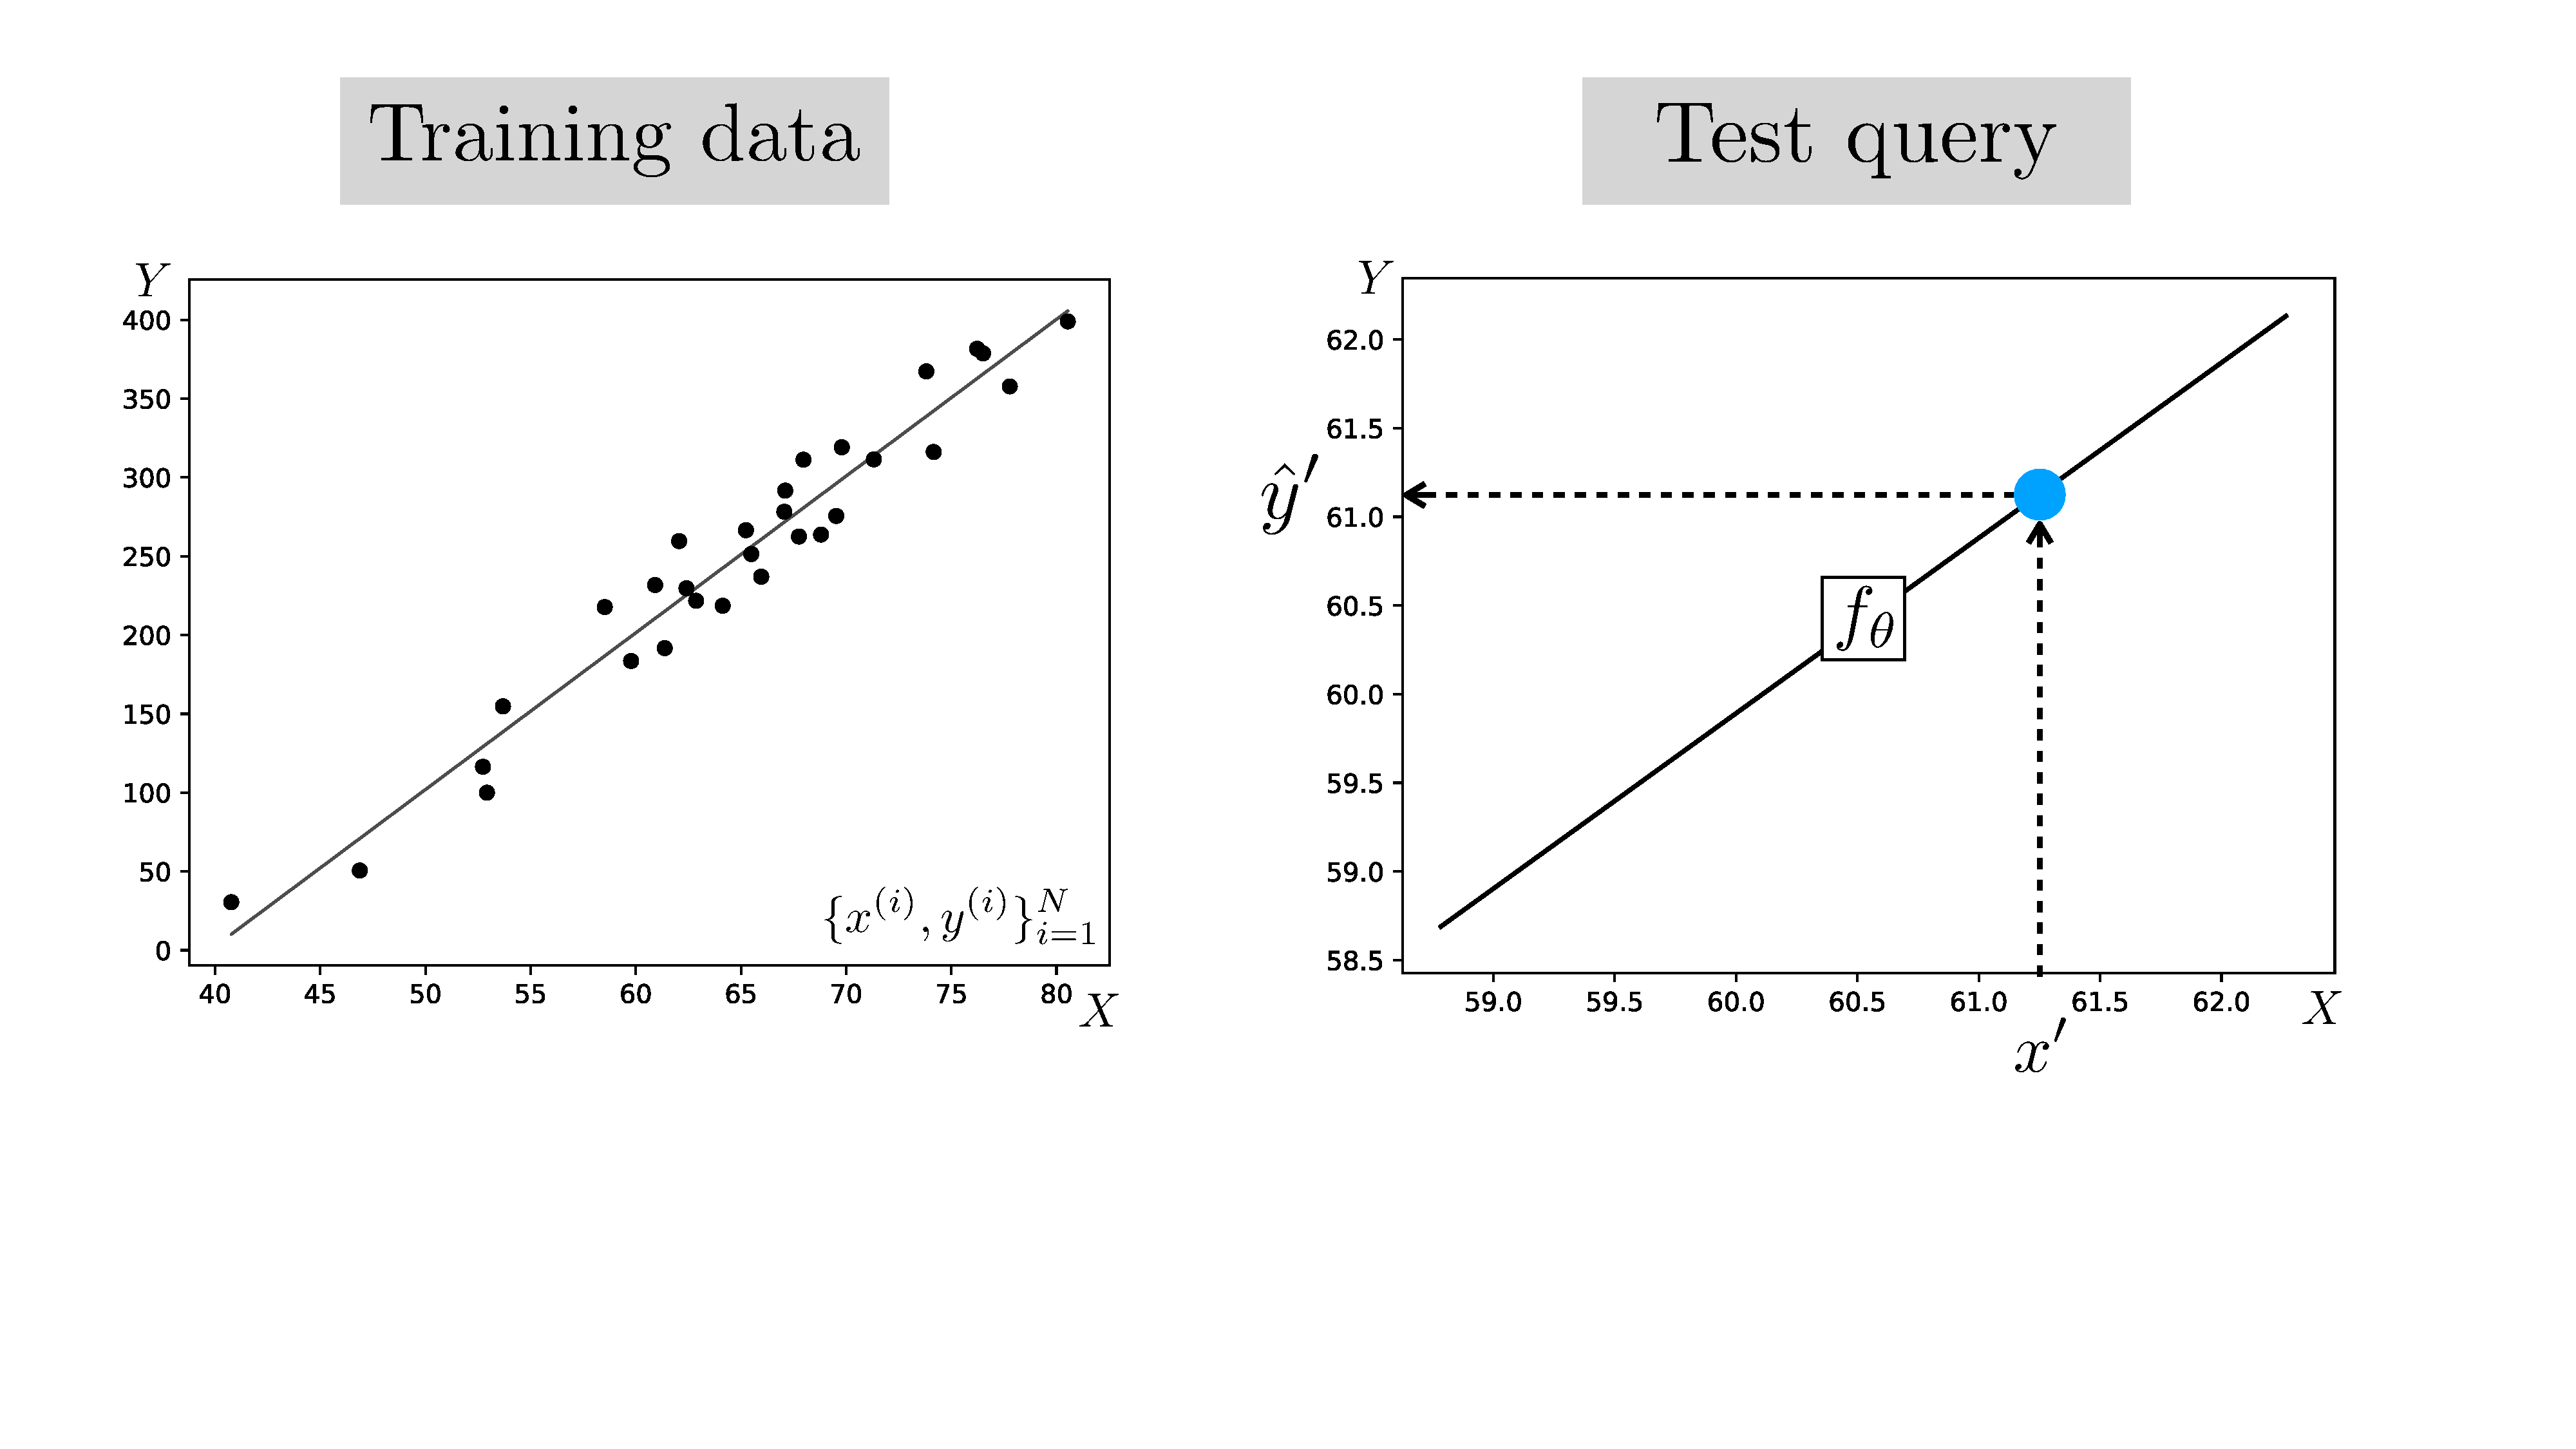
\includegraphics[width=1\linewidth]{./figures/intro_to_learning/ols_fit.pdf}
    }
    \caption{A best fit line is a visualization of a function $f_{\theta}$, that predicts the $y$-value for each input $x$-value.}
    \label{fig:intro_to_learning:ols_fit}
\end{figure}

We can now summarize the entire linear least-squares learning problem as follows:

\begin{center}
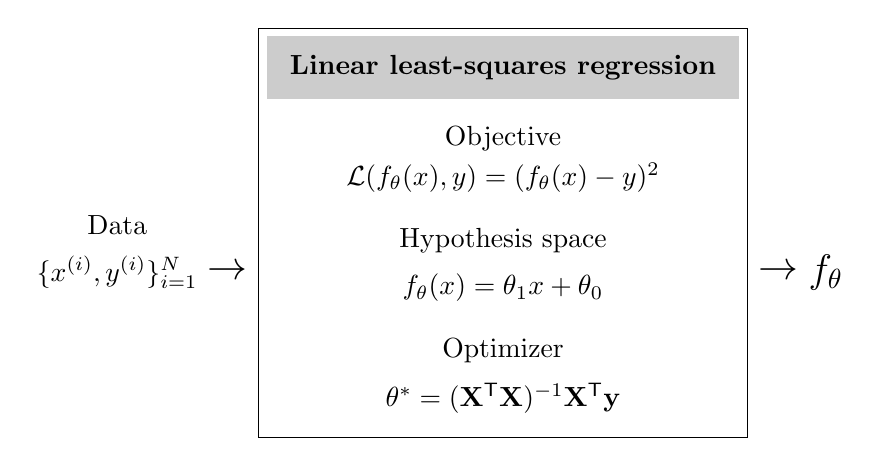
\begin{tikzpicture}
    \draw (0,0) rectangle (6.2,5.2); % outer box
    \fill[black!20] (0.1,4.3) rectangle (6.1,5.1); % gray box
    \node[] at (3.1,4.7) {{\bf Linear least-squares regression}};
    \node[] at (3.1,3.8) {Objective}; \node[] at (3.1,3.3) {$\mathcal{L}(f_{\theta}(x),y) = (f_{\theta}(x)-y)^2$};
    \node[] at (3.1,2.5) {Hypothesis space}; \node[] at (3.1,1.9) {$f_{\theta}(x) = \theta_1 x + \theta_0$};
    \node[] at (3.1,1.1) {Optimizer}; \node[] at (3.1,0.5) {$\theta^* = (\mathbf{X}^\transpose\mathbf{X})^{-1}\mathbf{X}^\transpose\mathbf{y}$};
    \node[] at (-1.8,2.7) {Data};
    \node[] at (-1.8,2.1) {$\{x^{(i)}, y^{(i)}\}_{i=1}^N$};
    \node[] at (-0.4,2.1) {{\Large  $ \rightarrow$}};
    \node[] at (7.2,2.1) {{\Large $f_{\theta}$}};
    \node[] at (6.6,2.1) {{\Large  $ \rightarrow$}};
\label{fig:ols_summary}
\end{tikzpicture}
\end{center}
% \begin{figure}[h]
%     \centering
%     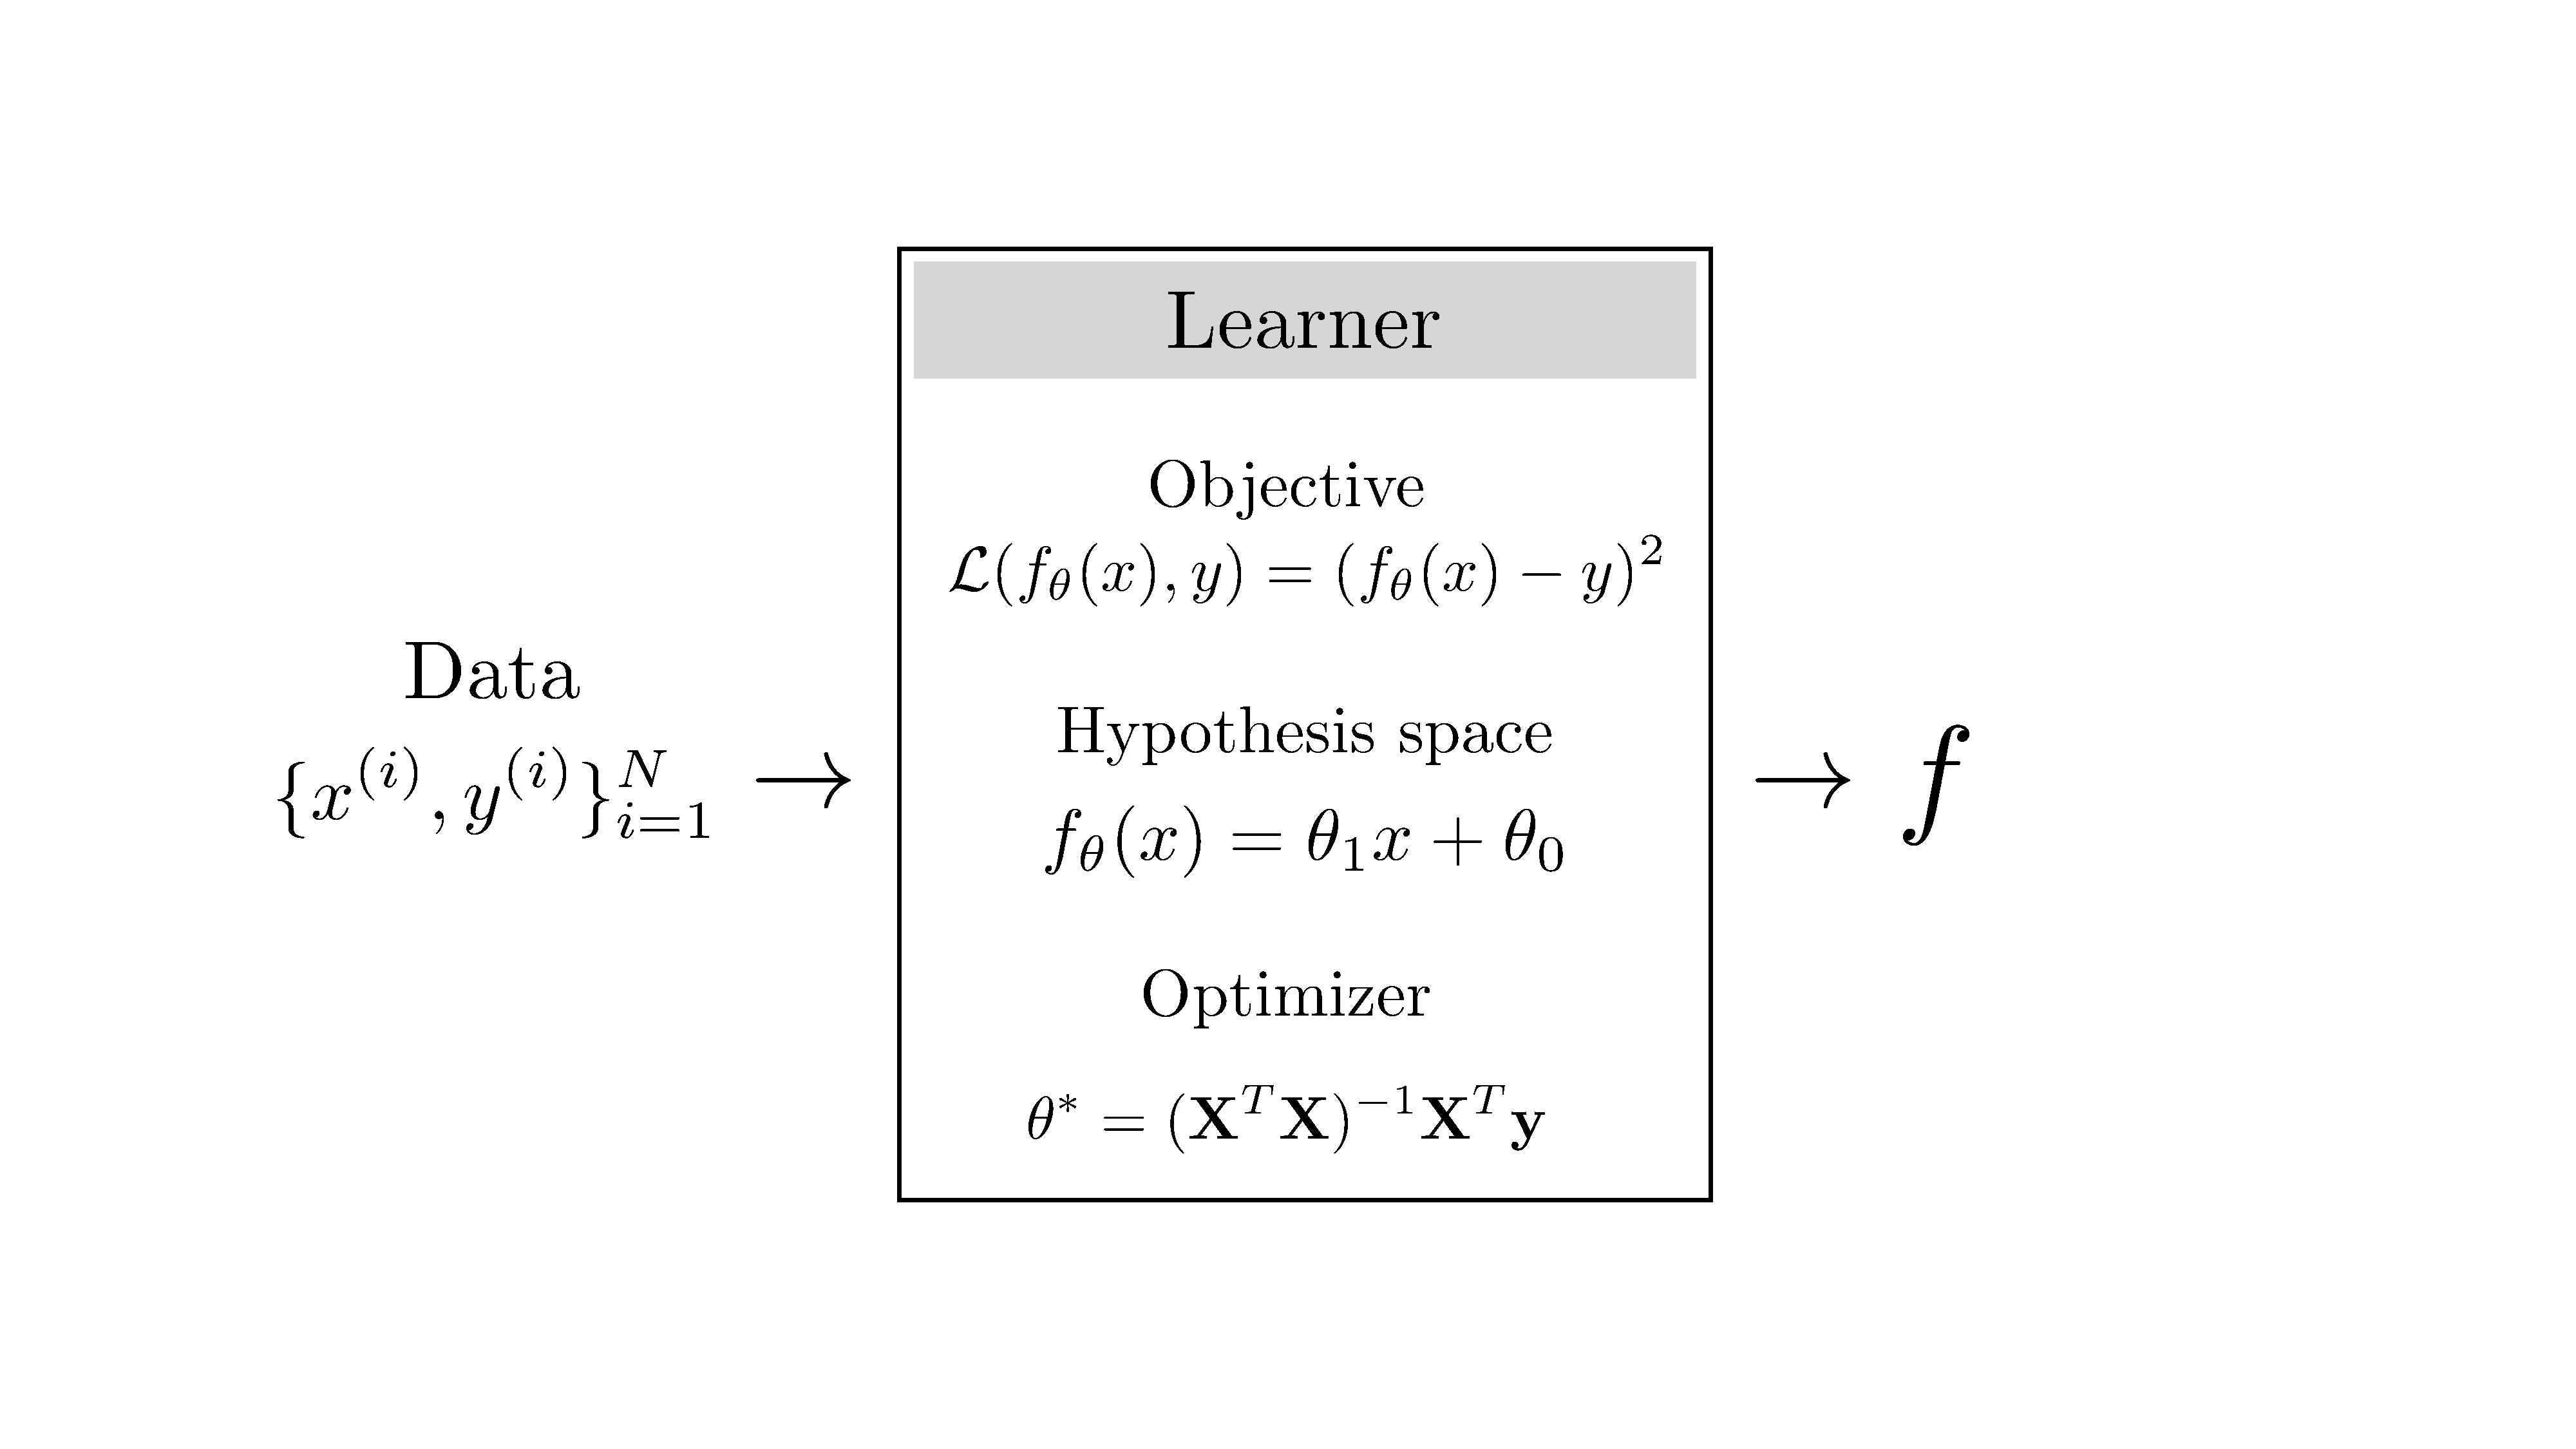
\includegraphics[width=0.6\linewidth]{./figures/intro_to_learning/ols_summary.pdf}
%     \label{fig:ols_summary}
% \end{figure}
\marginnote{In these diagrams, we will sometimes describe the objective just in terms of $\mathcal{L}$, in which case it should be understood that this implies $J(\theta) = \sum_{i=1}^N \mathcal{L}(f_{\theta}(x^{(i)}), y^{(i)})$.}[-4cm]

\subsection{Example 2: Program Induction}
At the other end of the spectrum we have what is known as \index{Program induction}\textbf{program induction}, which is one of the broadest classes of learning algorithm. In this setting, our hypothesis space may be all Python programs. Let's contrast linear least-squares with Python program induction. \Fig{\ref{fig:intro_to_learning:ols_system_diagram}} shows what linear least-squares looks like.

\begin{figure}[h]
    \centerline{
    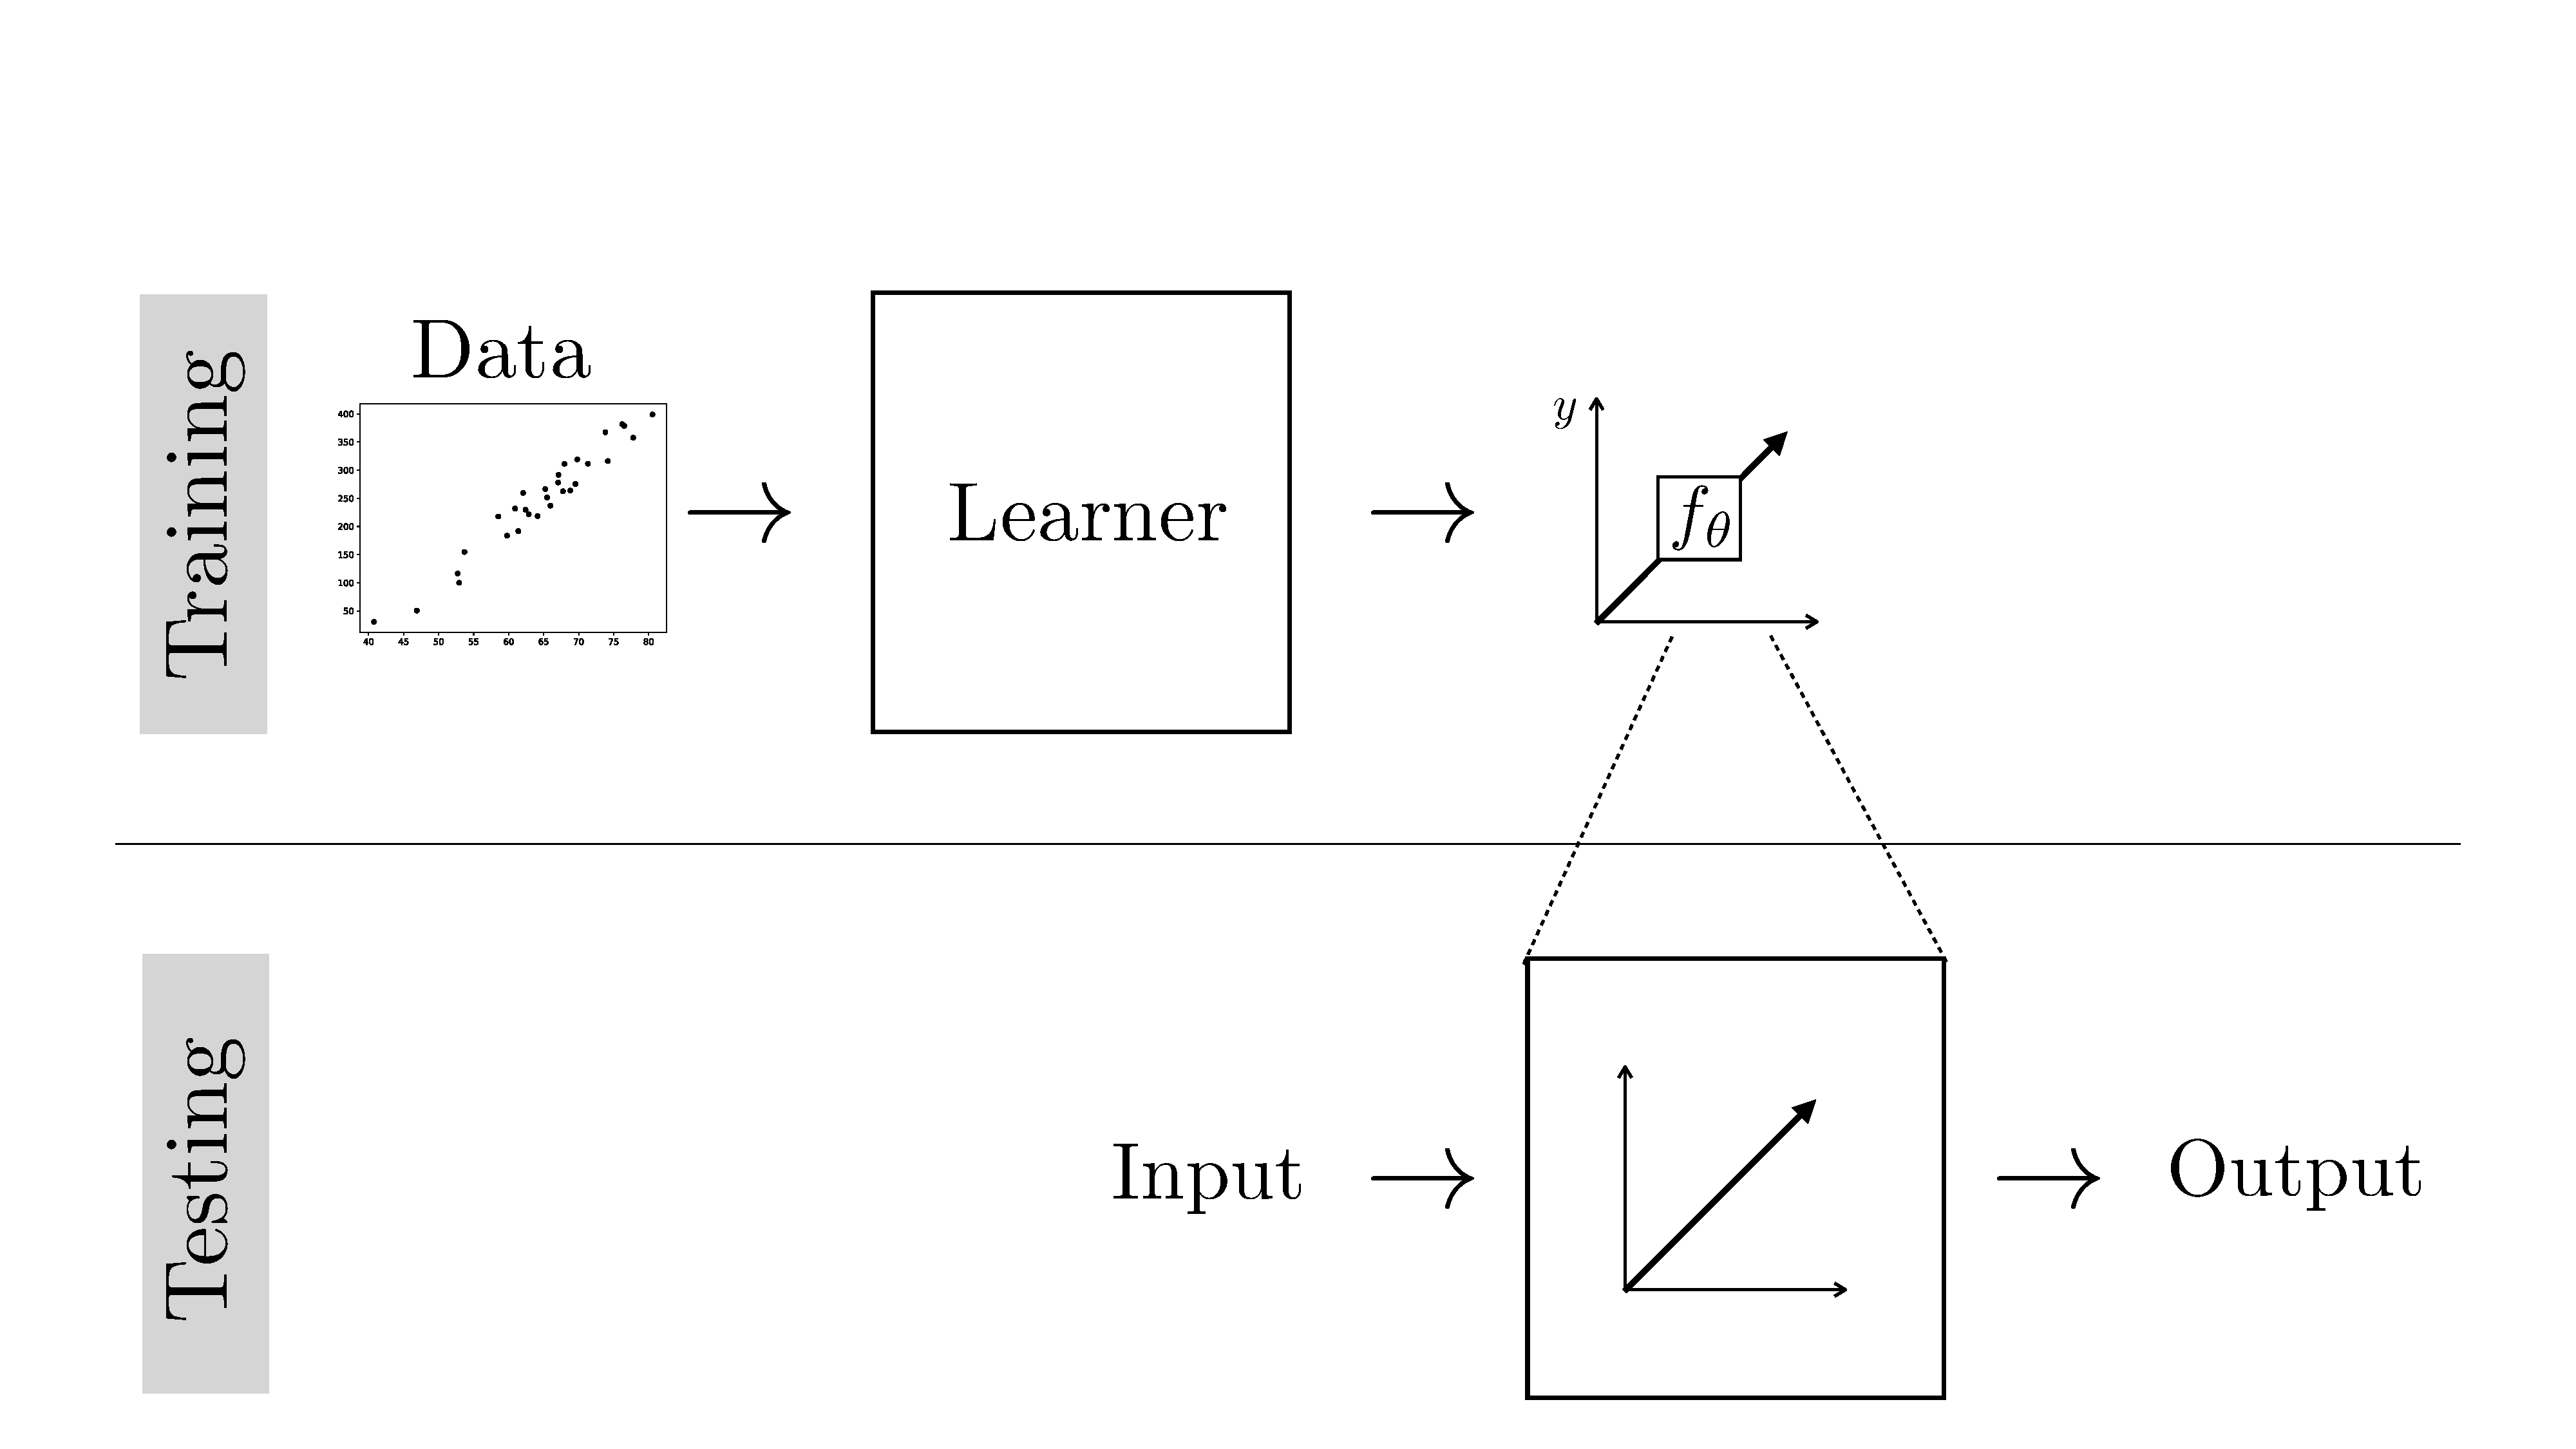
\includegraphics[width=0.8\linewidth]{./figures/intro_to_learning/ols_system_diagram.pdf}
    }
    \caption{Linear regression finds a line that predicts the training data's $y$-values from its $x$-values.}
    \label{fig:intro_to_learning:ols_system_diagram}
\end{figure}

The learned function is an algebraic expression that maps $x$ to $y$. Learning consisting of searching over two scalar parameters, $\theta_0$ and $\theta_1$.

\Fig{\ref{fig:intro_to_learning:program_induction_system_diagram}} shows Python program induction solving the same problem. In this case, the learned function is a Python program that maps $x$ to $y$. Learning consisted of searching over the space of all possible Python programs (within some max length). Clearly that's a much harder search problem than just finding two scalars. In \chap{\ref{chapter:problem_of_generalization}}, we will see some pitfalls of using too powerful a hypothesis space when a simpler one will do.

\begin{figure}[h]
    \centerline{
    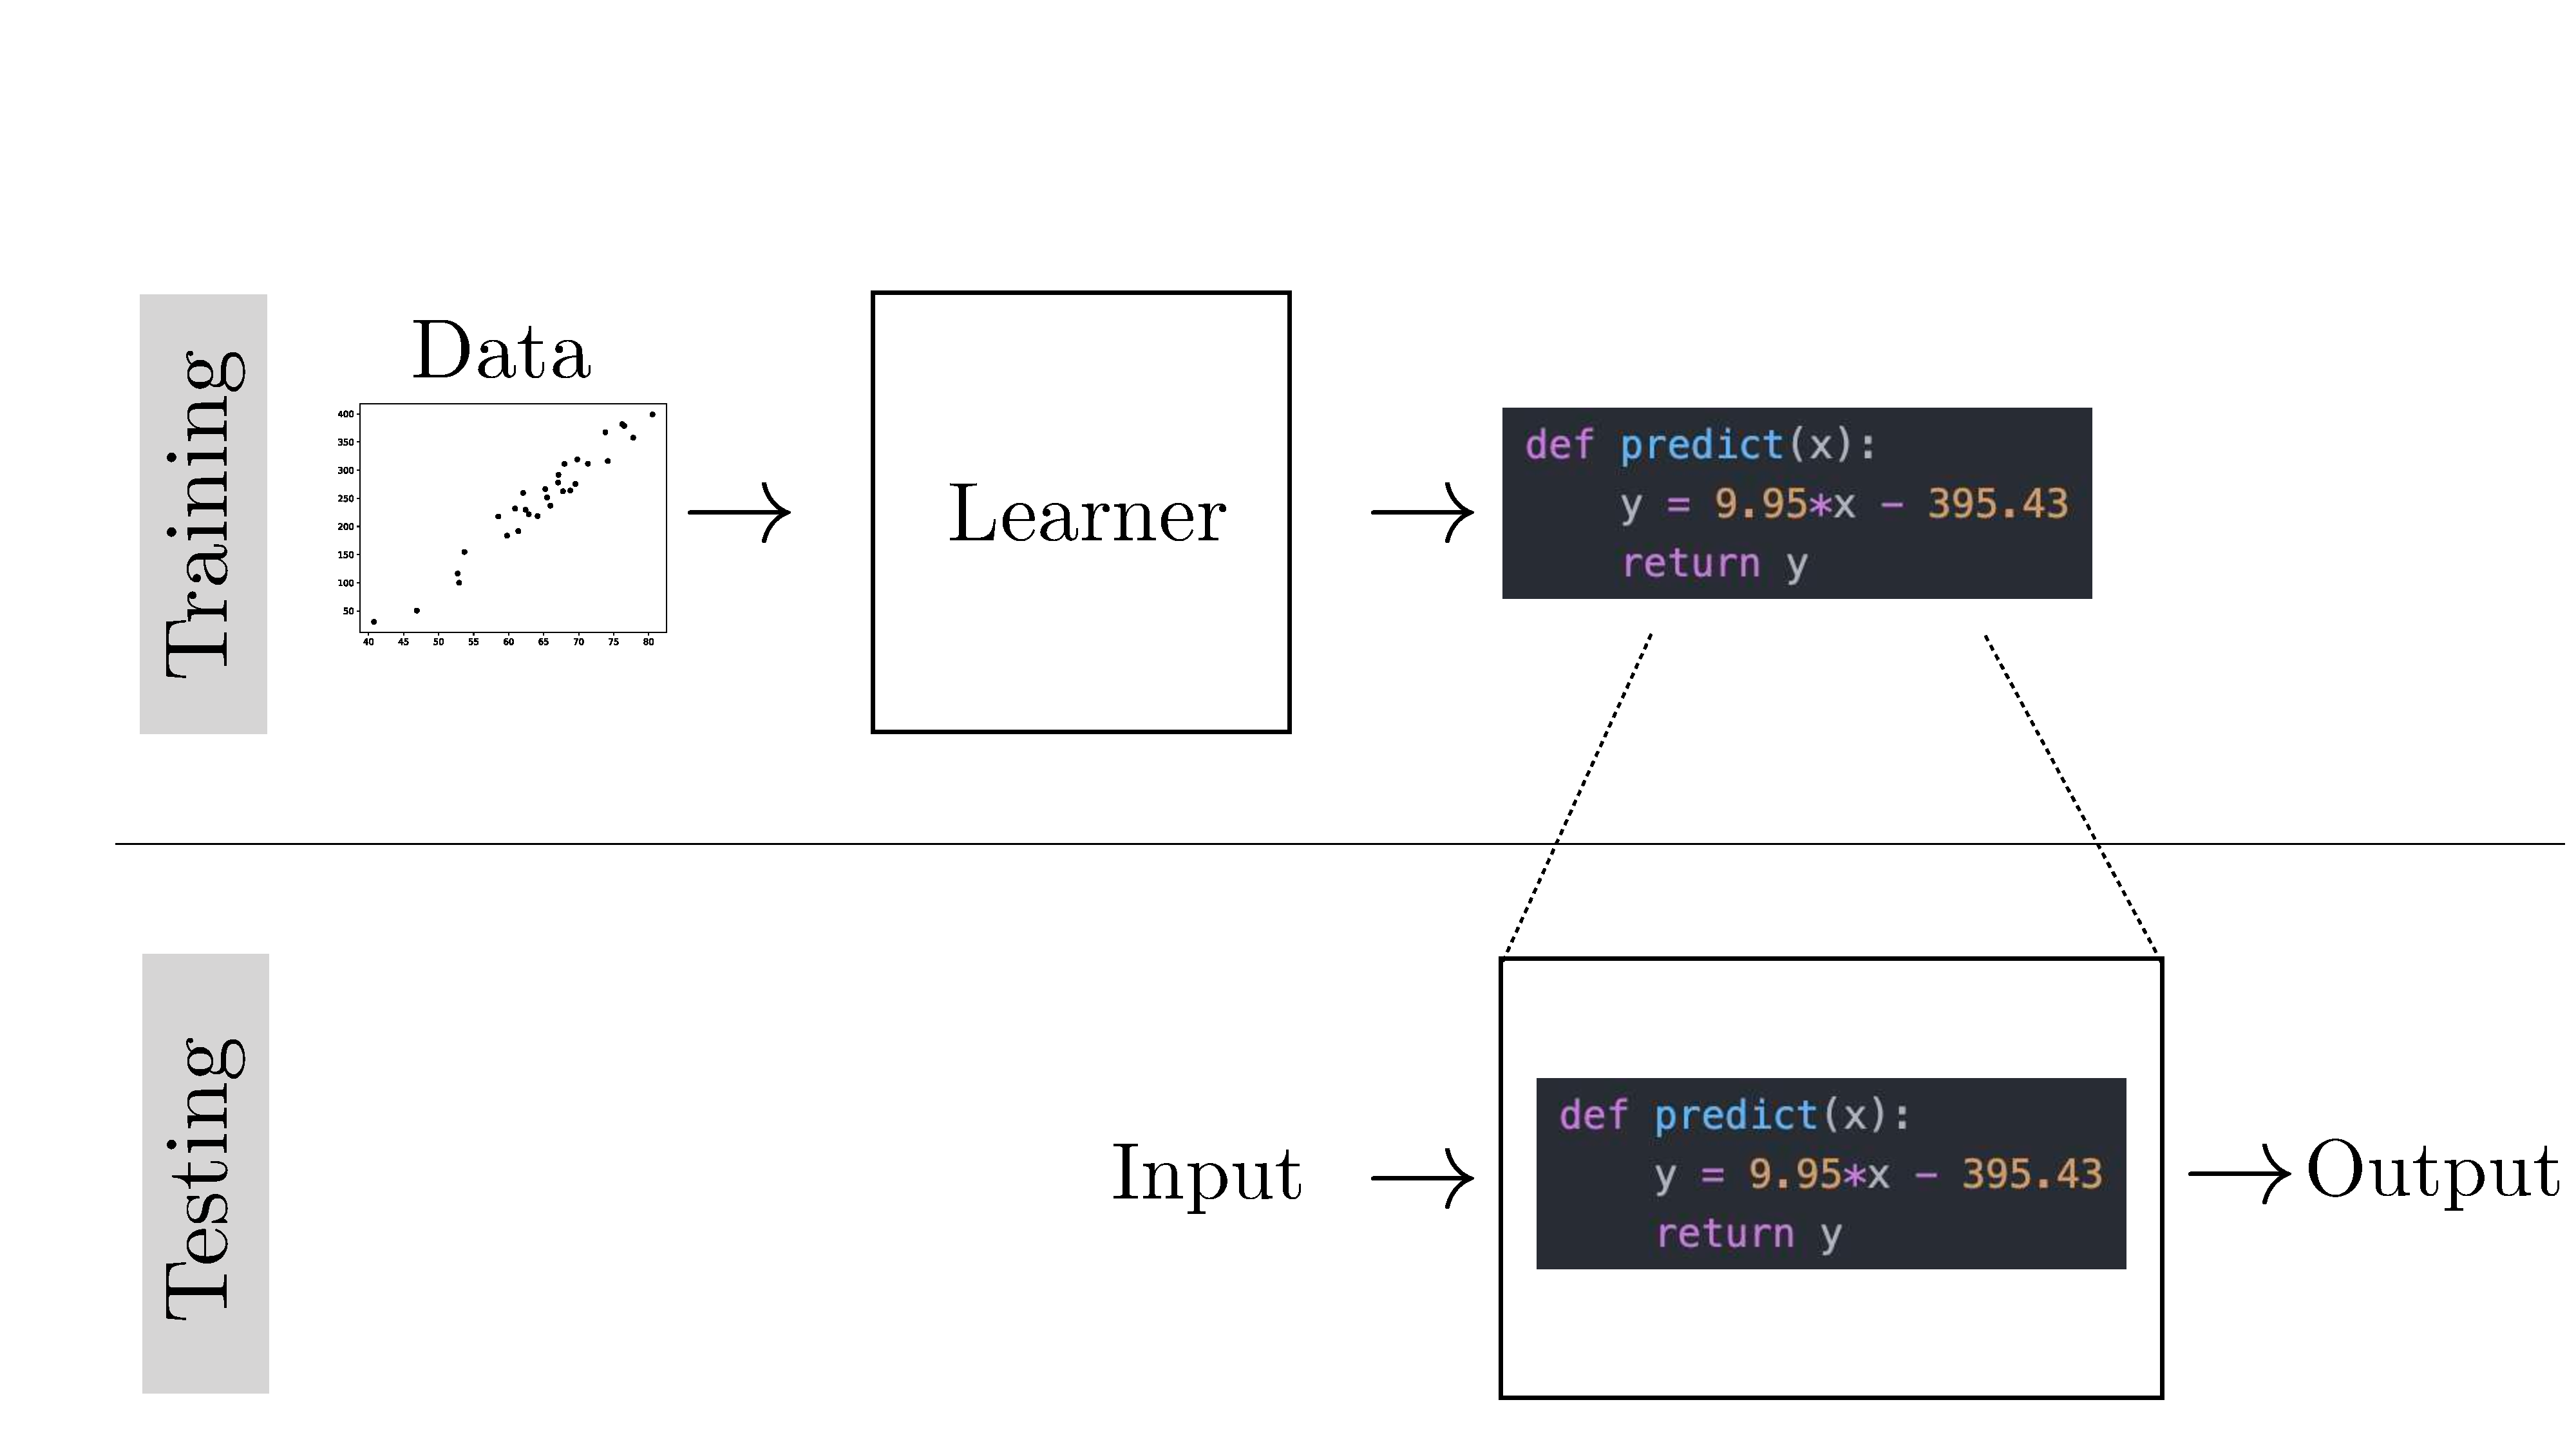
\includegraphics[width=0.8\linewidth]{./figures/intro_to_learning/program_induction_system_diagram.pdf}
    }
    \caption{Python program induction finds a Python program that predicts the training data's $y$-values from its $x$-values.}
    \label{fig:intro_to_learning:program_induction_system_diagram}
\end{figure}

\subsection{Example 3: Classification and Softmax Regression}\label{sec:intro_to_learning:image_classification}

A common problem in computer vision is to recognize objects. This is a \index{Classification}{\bf classification} problem. Our input is an image $\mathbf{x}$, and our target output is a class label $\mathbf{y}$ (\fig{\ref{fig:intro_to_learning:image_classification}}).

\begin{figure}[h]
    \centerline{
    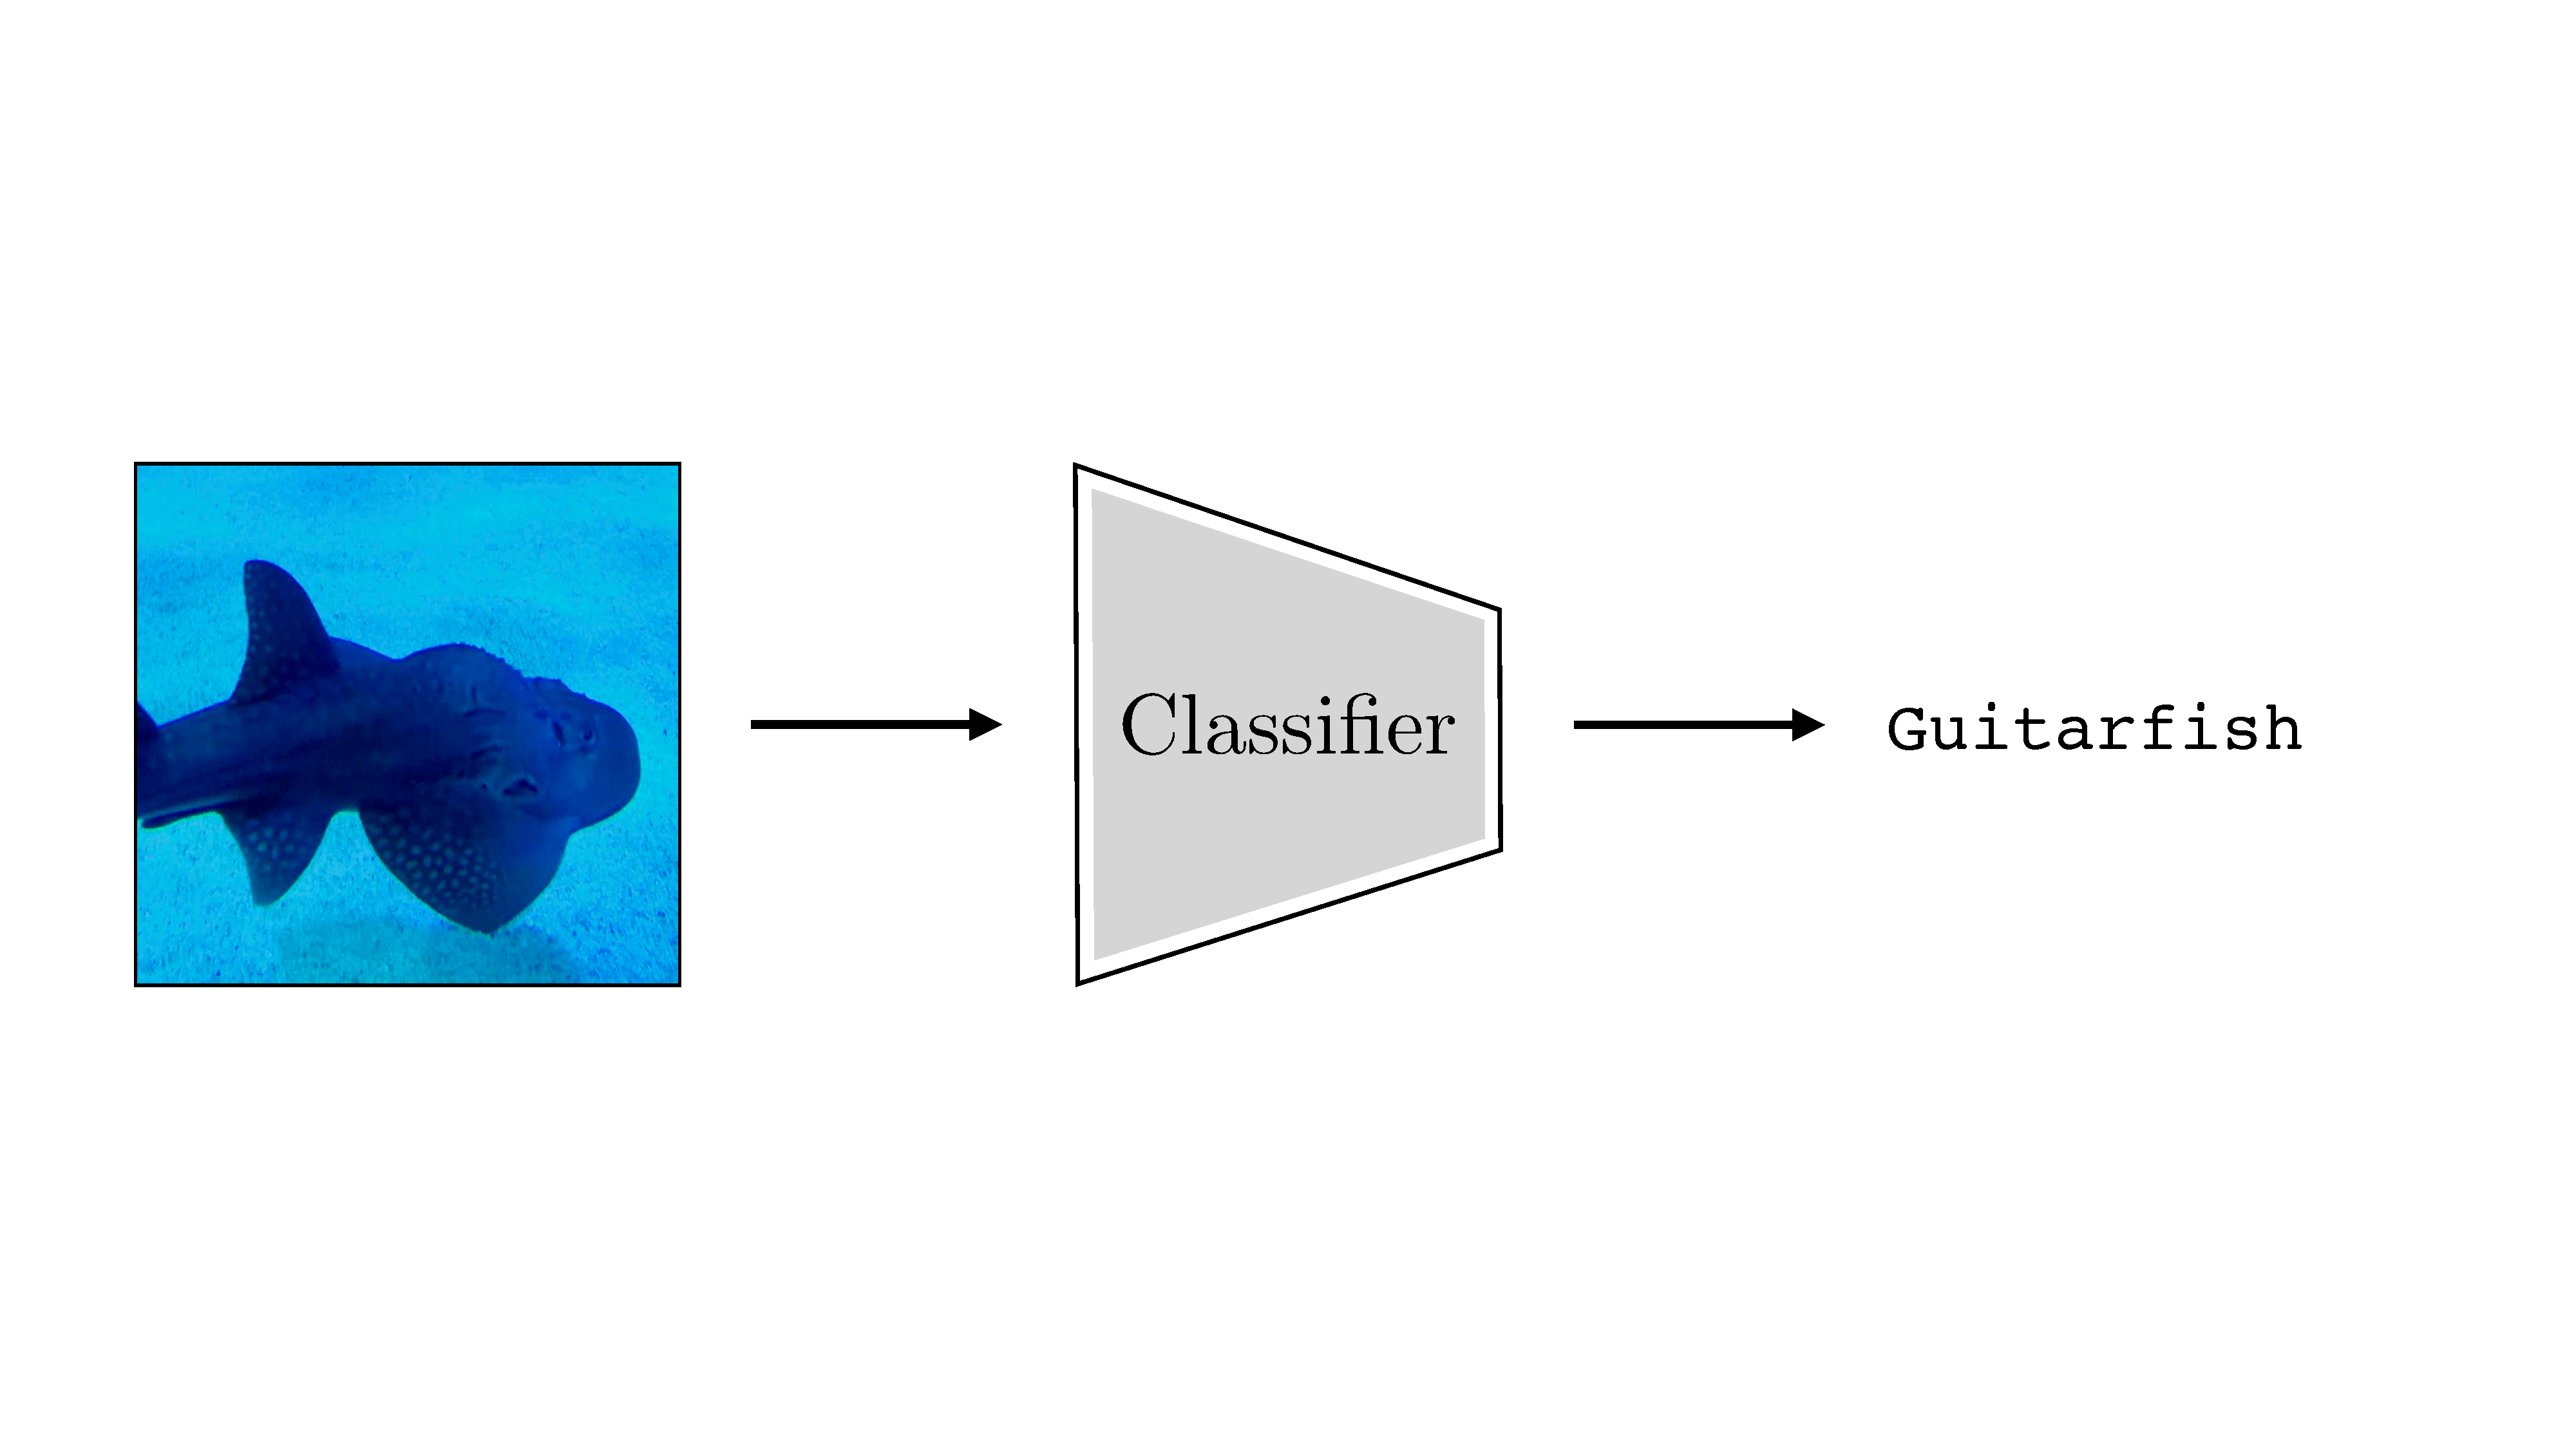
\includegraphics[width=0.7\linewidth]{./figures/intro_to_learning/image_classification.pdf}
    }
    \caption{Image classification.}
    \label{fig:intro_to_learning:image_classification}
\end{figure}

How should we formulate this task as a learning problem? The first question is how do we even represent the input and output? Representing images is pretty straightforward; as we have seen elsewhere in this book, they can be represented as arrays of numbers representing red-green-blue colors: $\mathbf{x} \in \mathbb{R}^{H \times W \times 3}$, where $H$ is image height and $W$ is image width.

How can we represent class labels? It turns out a convenient representation is to let $\mathbf{y}$ be a $K$-dimensional vector, for $K$ possible classes, with $y_k = 1$ if $\mathbf{y}$ represents class $k$, and $y_k = 0$ otherwise. This representation is called a \index{One-hot code}\textbf{one-hot code}, since just one element of the vector is on (``hot''). Each class has a unique one-hot code. We will see why this representation makes sense shortly. The one-hot codes are the targets for the function we are learning. Our goal is to learn a function $f_{\theta}$ that output vectors $\hat{\mathbf{y}}$ that match the one-hot codes, thereby correctly classifying the input images.
%So the learning problem is to map $f_{\theta}: \mathbb{R}^{H \times W \times 3} \rightarrow \mathbb{R}^K$. 
\marginnote{An example of one-hot codes for representing $K$=5 different classes:
\\[6pt]
\centerline{
\includegraphics[width=0.275\linewidth]{figures/intro_to_learning/one_hot_codes_white.eps}
}
}[-1.8cm]

Next, we need to pick a loss function. Our first idea might be that we should minimize misclassifications. That would correspond to the so called \index{0-1 loss}{\bf 0-1 loss}:
\begin{align}
    \mathcal{L}(\hat{\mathbf{y}},\mathbf{y}) = \mathbbm{1}(\hat{\mathbf{y}}\neq\mathbf{y}),
\end{align}
where $\mathbbm{1}$ is the indicator function that evaluates to 1 if and only if its argument is true, and 0 otherwise. Unfortunately, minimizing this loss is a discrete optimization problem, and it is NP-hard. Instead, people commonly use the \index{Cross-entropy loss}{\bf cross-entropy loss}, which is continuous and differentiable (making it easier to optimize):
\begin{align}
    \mathcal{L}(\hat{\mathbf{y}},\mathbf{y}) = H(\mathbf{y}, \hat{\mathbf{y}}) = - \sum_{k=1}^K y_k \log \hat{y}_k \quad\quad \triangleleft \quad \text{cross-entropy loss}
\end{align}
The way to think about this is $\hat{y}_k$ should \textit{represent the probability} we think the image is an image of class $k$. Under that interpretation, minimizing cross-entropy maximizes the log likelihood of the ground truth observation $\mathbf{y}$ under our model's prediction $\hat{\mathbf{y}}$.

For that interpretation to be valid, we require that $\hat{\mathbf{y}}$ represent a \index{Probability mass function}{\bf probability mass function} ({\bf pmf}). A pmf $\mathbf{p}$, over $K$ classes, is defined as a $K$-dimensional vector with elements in the range $[0,1]$ that sums to 1. In other words, $\mathbf{p}$ is a point on the $(K-1)$-\textbf{simplex}, which we denote as \index{Simplex}$\mathbf{p} \in \vartriangle^{K-1}$.\marginnote{The $(K-1)$-simplex, $\vartriangle^{K-1}$, is the set of all $K$-dimensional vectors whose elements sum to 1. $K$-dimensional one-hot codes live on the vertices of $\vartriangle^{K-1}$.}[-1.0cm]

To ensure that the output of our learned function $f_{\theta}$ has this property, i.e., $f_{\theta} \in \vartriangle^{K-1}$, we can compose two steps: (1) first apply a function $z_{\theta}: \mathcal{X} \rightarrow \mathbb{R}^K$, (2) then squash the output into the range $[0,1]$ and normalize it to sum to 1. 
%So, if our parameterized function outputs a vector $f_{\theta}(\mathbf{x}) \in \mathbb{R}^K$, then we can convert it to a pmf by squashing it into the range $[0,1]$ and normalizing it to sum to 1. 
A popular way to squash is via the \index{Softmax}{\bf softmax} function:\marginnote{Using softmax is a modeling choice; we could have used any function that squashes into a valid pmf, that is, a nonnegative vector that sums to 1.}[0.8cm]
\begin{align}
    &\mathbf{z} = z_{\theta}(\mathbf{x})\\
    &\hat{\mathbf{y}} = \texttt{softmax}(\mathbf{z})\\
    &\quad \quad \hat{y}_j = \frac{e^{-z_j}}{\sum_{i=1}^K e^{-z_k}}.
\end{align}
The values in $\mathbf{z}$ are called the \index{Logits}\textbf{logits} and can be interpreted as the unnormalized log probabilities of each class. 
Now we have,
\begin{align}
    \hat{\mathbf{y}} = f_{\theta}(\mathbf{x}) = \texttt{softmax}(z_{\theta}(\mathbf{x}))
\end{align}
\Fig{\ref{fig:softmax_regression_diagram}} shows what the variables look like for processing one photo of a fish during training.

\begin{figure}[h]
    \centering
    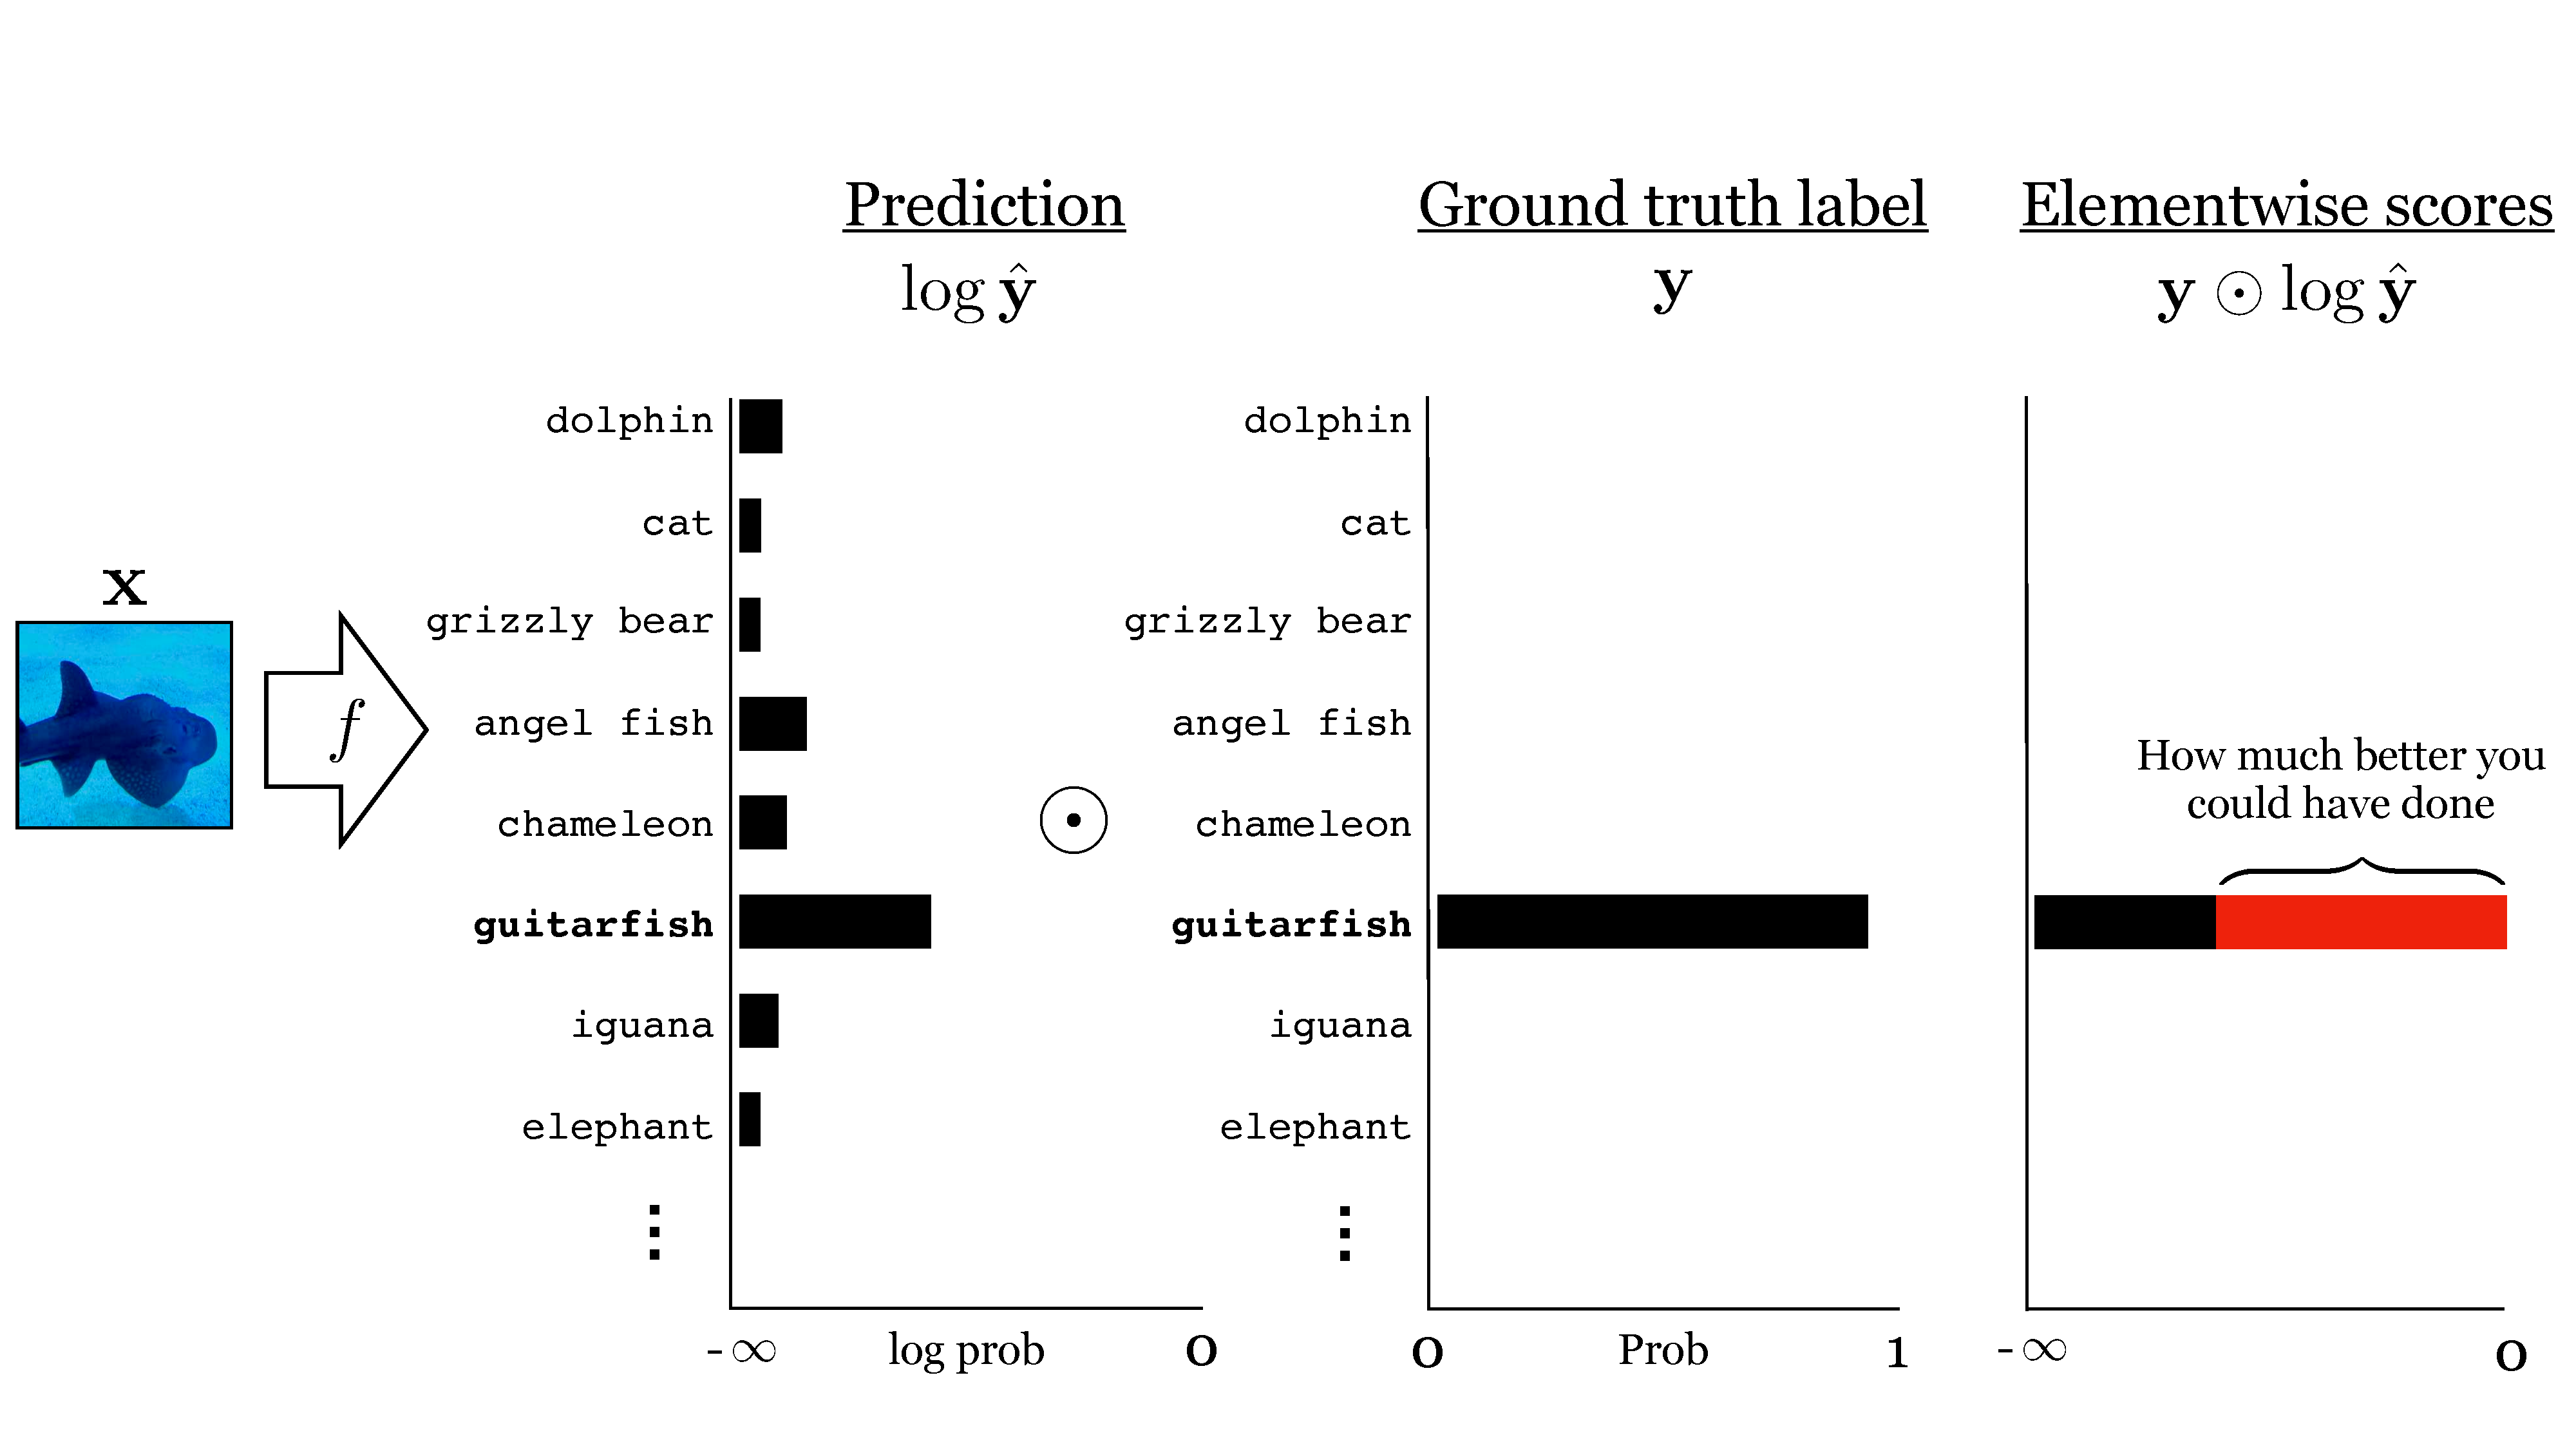
\includegraphics[width=1.0\linewidth]{./figures/intro_to_learning/softmax_regression_diagram.pdf}
    \caption{Softmax regression for image classification. The $\odot$ symbol represents an elementwise product. The cross-entropy loss is the negative of the sum over elementwise agreements between the prediction vector $\hat{\mathbf{y}}$ and the label vector $\mathbf{y}$, that is, if $\mathbf{s} = \mathbf{y} \odot \log \hat{\mathbf{y}}$ is the vector of scores for how well our prediction agrees with the label, then our cross-entropy loss is $H(\mathbf{y}, \hat{\mathbf{y}}) = - \sum_{k=1}^K s_k$.}
    \label{fig:softmax_regression_diagram}
\end{figure}

The prediction placed about 40 percent probability on the true class, ``guitarfish,'' so we are 60 percent off from an ideal prediction (indicated by the red bar; an ideal prediction would place 100 percent probability on the true class). Our loss is $-\log 0.4$.

This learning problem, which is also called \index{Softmax regression}{\bf softmax regression}, can be summarized as follows:\marginnote{Softmax regression is just one way to model a classification problem. We could have made other choices for how to map input data to class labels.}[-0.4cm]

\begin{center}
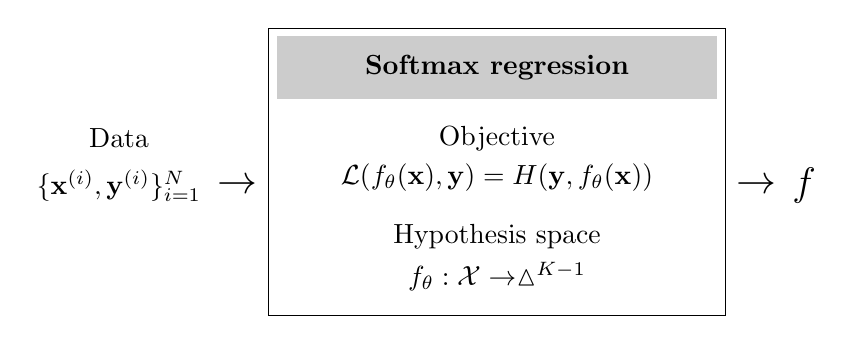
\begin{tikzpicture}
    \draw (0,-1.25) rectangle (5.8,2.4); % outer box
    \fill[black!20] (0.1,1.5) rectangle (5.7,2.3); % gray box
    \node[] at (2.9,1.9) {{\bf Softmax regression}};
    \node[] at (2.9,1.0) {Objective}; \node[] at (2.9,0.5) {$\mathcal{L}(f_{\theta}(\mathbf{x}), \mathbf{y}) = H(\mathbf{y}, f_{\theta}(\mathbf{x}))$};
    \node[] at (2.9,-0.25) {Hypothesis space}; \node[] at (2.9,-0.75) {$f_{\theta}: \mathcal{X} \rightarrow \vartriangle^{K-1}$};
    \node[] at (-1.9,1.0) {Data};
    \node[] at (-1.9,0.4) {$\{\mathbf{x}^{(i)}, \mathbf{y}^{(i)}\}_{i=1}^N$};
    \node[] at (-0.4,0.4) {{\Large  $ \rightarrow$}};
    \node[] at (6.8,0.4) {{\Large $f$}};
    \node[] at (6.2,0.4) {{\Large  $ \rightarrow$}};
\label{fig:softmax_regression_learning_problem}
\end{tikzpicture}
\end{center}
% \begin{figure}[h]
%     \centering
%     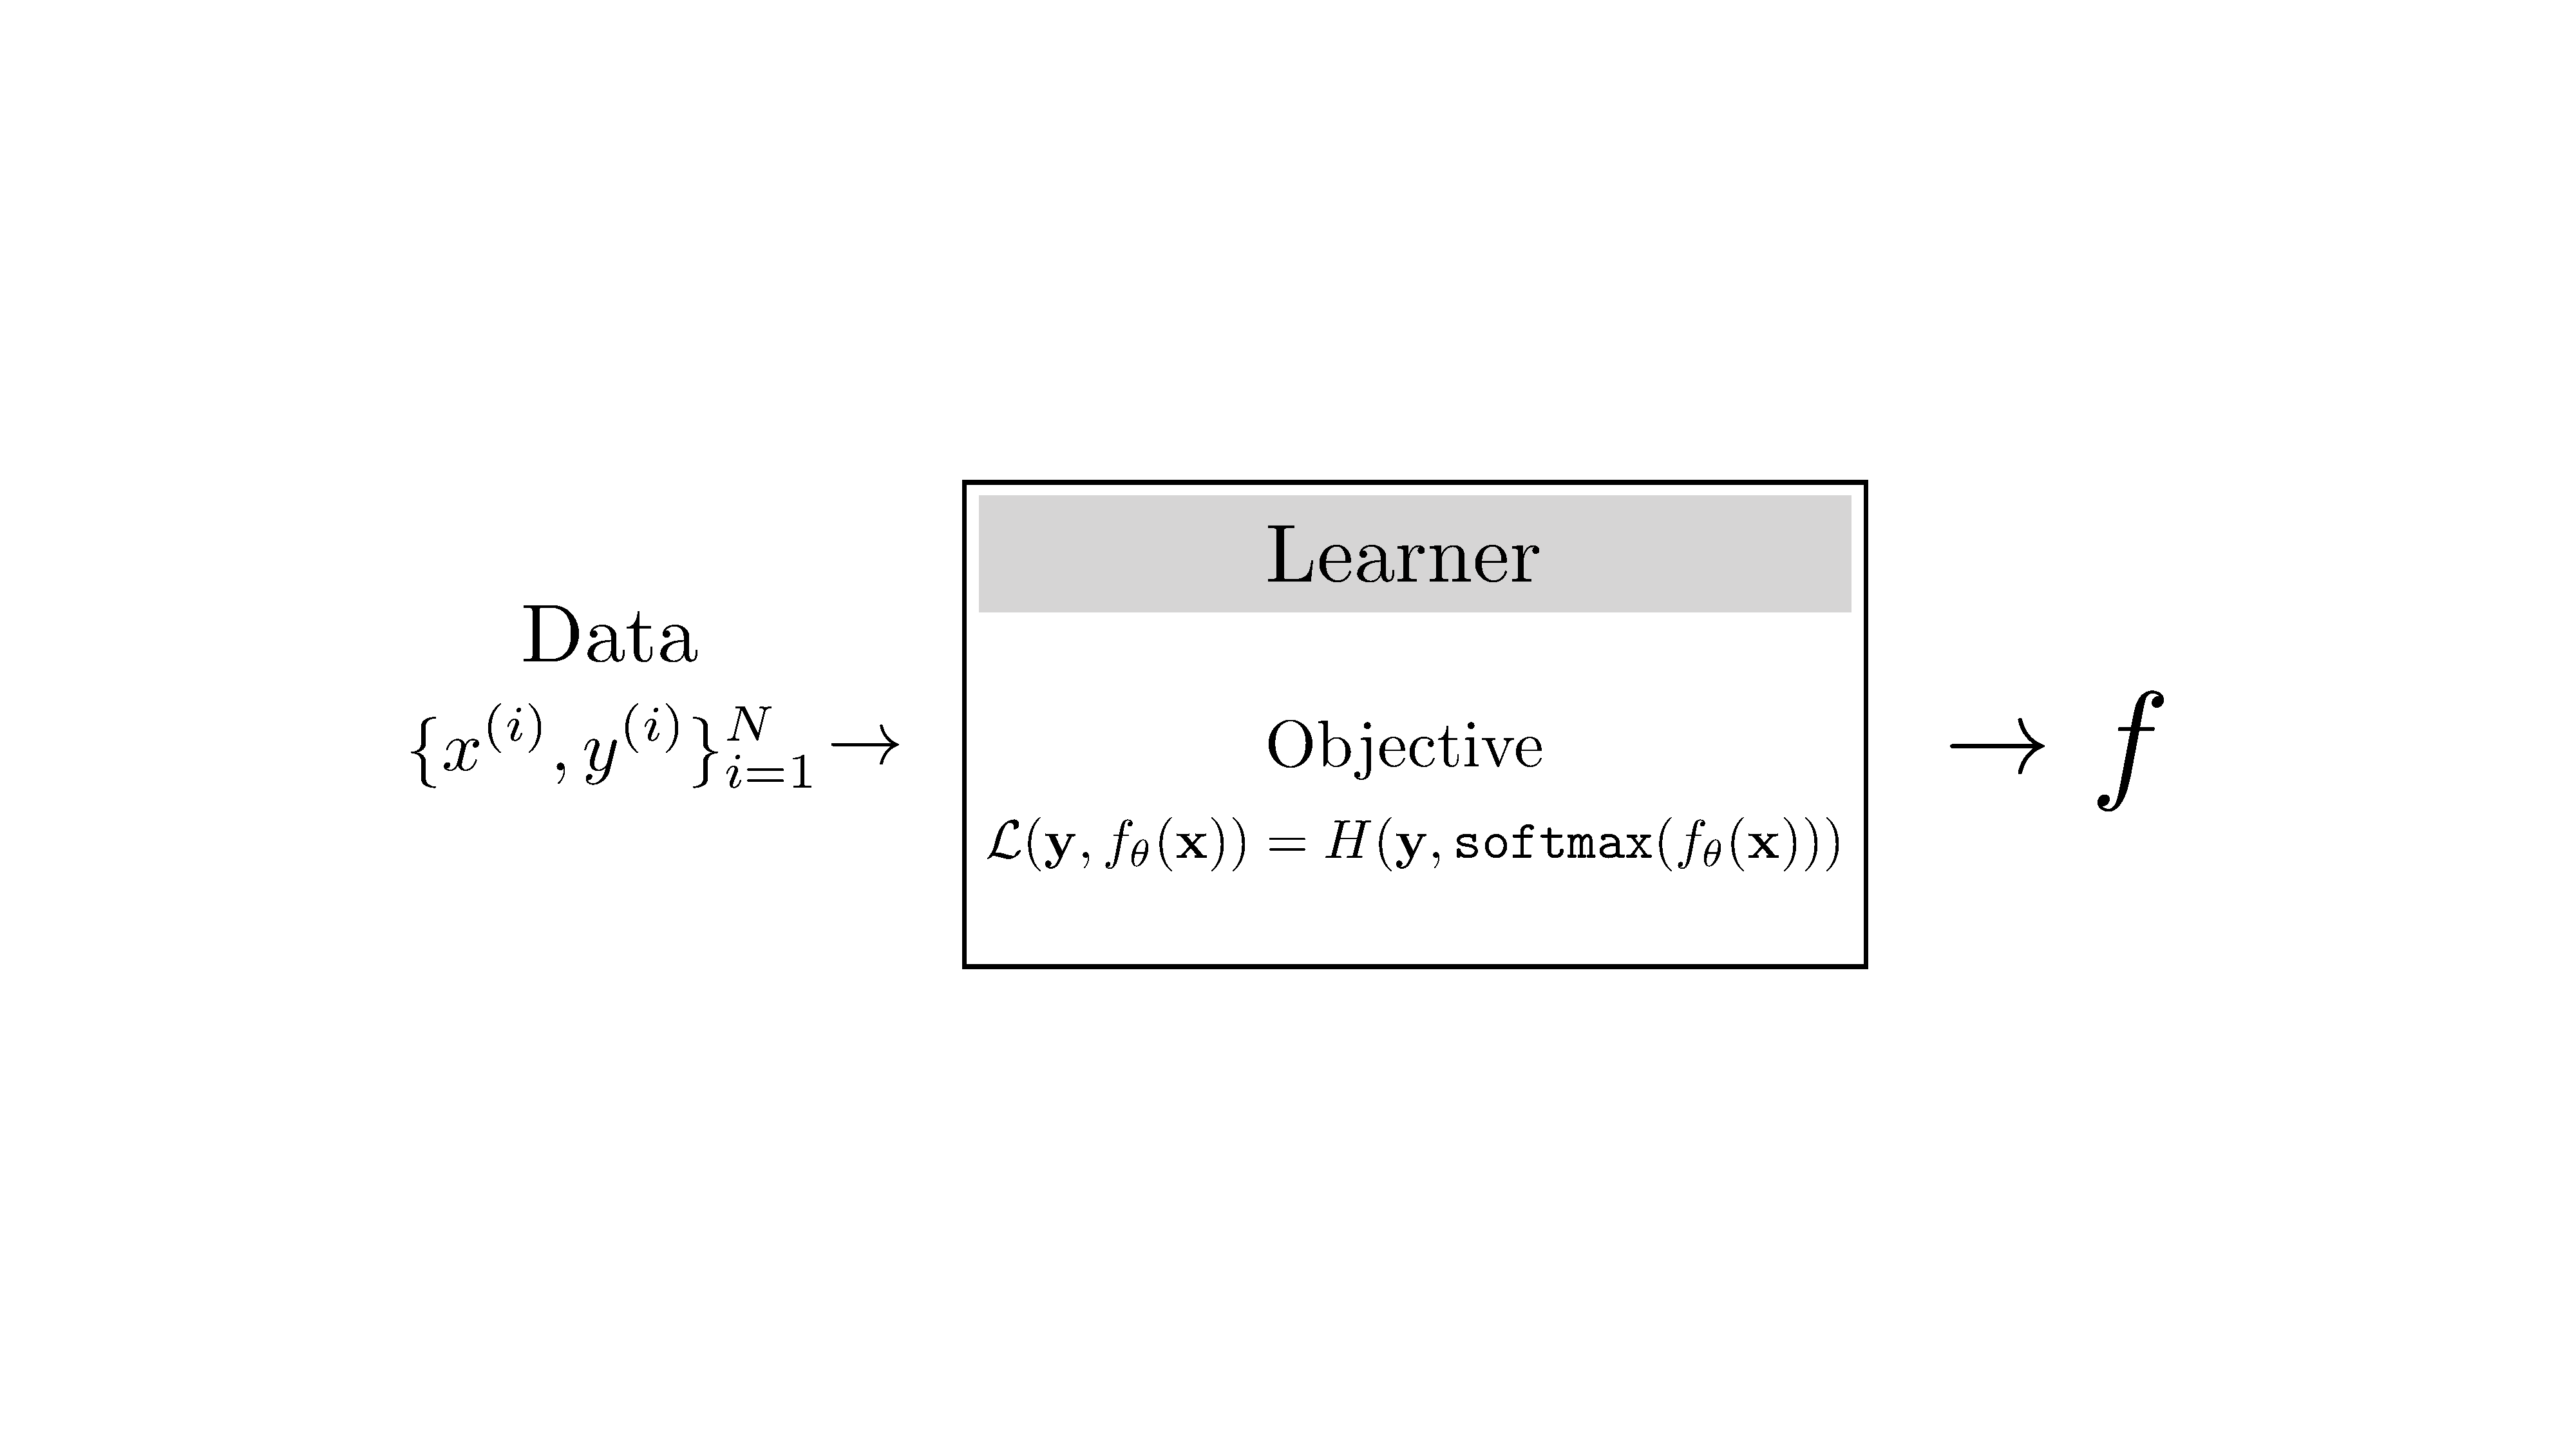
\includegraphics[width=0.7\linewidth]{./figures/intro_to_learning/softmax_regression_learning_problem.pdf}
%     \label{fig:softmax_regression_learning_problem}
% \end{figure}
Notice that we have left the hypothesis space only partially specified, and we left the optimizer unspecified. This is because softmax regression refers to the whole family of learning methods that have this general form. This is one of the reasons we conceptualized the learning problem in terms of the three key ingredients described previously: you can often develop them each in isolation, then mix and match.

%\#1 specifies the ``hypothesis space" (aka ``model class") we will search over. A simple model class would be ``linear functions". A more complex model class might be ``C++ programs". \#2 specifies the ``objective function" we wish to optimize. Suppose we are trying to predict tomorrow's weather. Then a natural objective would be that our prediction is close to the truth, for example, we could measure the Euclidean distance between our prediction of the temperature and what its actual value turns out to be. If we use linear functions for our model class, and Euclidean distance for our objective function, then we get what is known as a ``linear least squares" problem. 

%The final question, \#3, is how do we search over the model class to find the instantiation that optimizes the objective? One common approach is hill climbing: starting with some initial parameters, adjust them slightly in the direction that locally improves the objective. Hill climbing can be done by trial and error -- make random adjustments and keep the ones that improved the score -- or by gradient ascent -- use the derivative of the objective function with respect to the parameters to determine the adjustment that will locally increase the objective the most.

%For most of the rest of this class, we will consider machine learning algorithms that answer these three questions as follows:
%\begin{enumerate}
%    \item Hypothesis space: deep neural nets
%    \item Objective: predictions should be close to the truth
%    \item Optimizer: gradient descent
%\end{enumerate}

%What remains is to investigate each of these components in detail.



%\section{Reinforcement learning}
%{\bf Reinforcement learning} is a term that means many different things to different people. A classic definition is learners whose objective is to optimize a {\bf reward function}, rather than to fit a model to examples. A reward function is a mapping from outputs to scores: $r: Y \rightarrow \mathbb{R}$. The learning tries to come up with a function that maximizes rewards.

%However, there is another special distinction of reinforcement learning, and in my opinion a more important distinction: reinforcement learning deals with the setting where data is a function of the learned policy.

%\marginnote{In fact, most terms in machine learning do not have precise, agreed upon definitions. Instead they refer to a collection of connotations, and these connotations will be different in different communities.}[-1.83cm]

%\section{Unsupervised learning}


\section{Learning to Learn}% {\small [Advanced topic]}}

Learning to learn, also called \index{Metalearning}{\bf metalearning}, is a special case of learning where the hypothesis space is learning algorithms. 

Recall that learners train on past instances of a problem to produce an algorithm that can solve future instances of the problem. The goal of metalearning is to handle the case where the future problem we will encounter is itself a learning problem, such as ``find the least-squares line fit to these data points.'' One way to train for this would be by example. Suppose that we are given the following \{\texttt{input}, \texttt{output}\} examples:
\begin{align}
    &\{\texttt{input:} \big(x:[1,2], y:[1,2]\big), &&\texttt{output:} y = x\}\nonumber \\
    &\{\texttt{input:} \big(x:[1,2], y:[2,4]\big), &&\texttt{output:} y = 2x\}\nonumber \\
    &\{\texttt{input:} \big(x:[1,2], y:[0.5,1]\big), &&\texttt{output:} y = \frac{x}{2}\}\nonumber
\end{align}
These are examples of performing least-squares regression; therefore the learner can fit these examples by learning to perform least-squares regression.\marginnote{Note that least-squares regression is not the unique solution that fits these examples, and the metalearner might arrive at a different solution that fits equally well.}[-0.8cm] Since least-squares regression is itself a learning algorithm, we can say that the learner learned to learn.

We started this chapter by saying the learning is a meta-algorithm: it's an algorithm that outputs an algorithm. Metalearning is a meta-meta-algorithm and we can visualize it by just adding another outer loop on top of a learner, as shown in \fig{\ref{fig:intro_to_learning:meta_learning_diagram}}.
\begin{figure}[h]
    \centerline{
    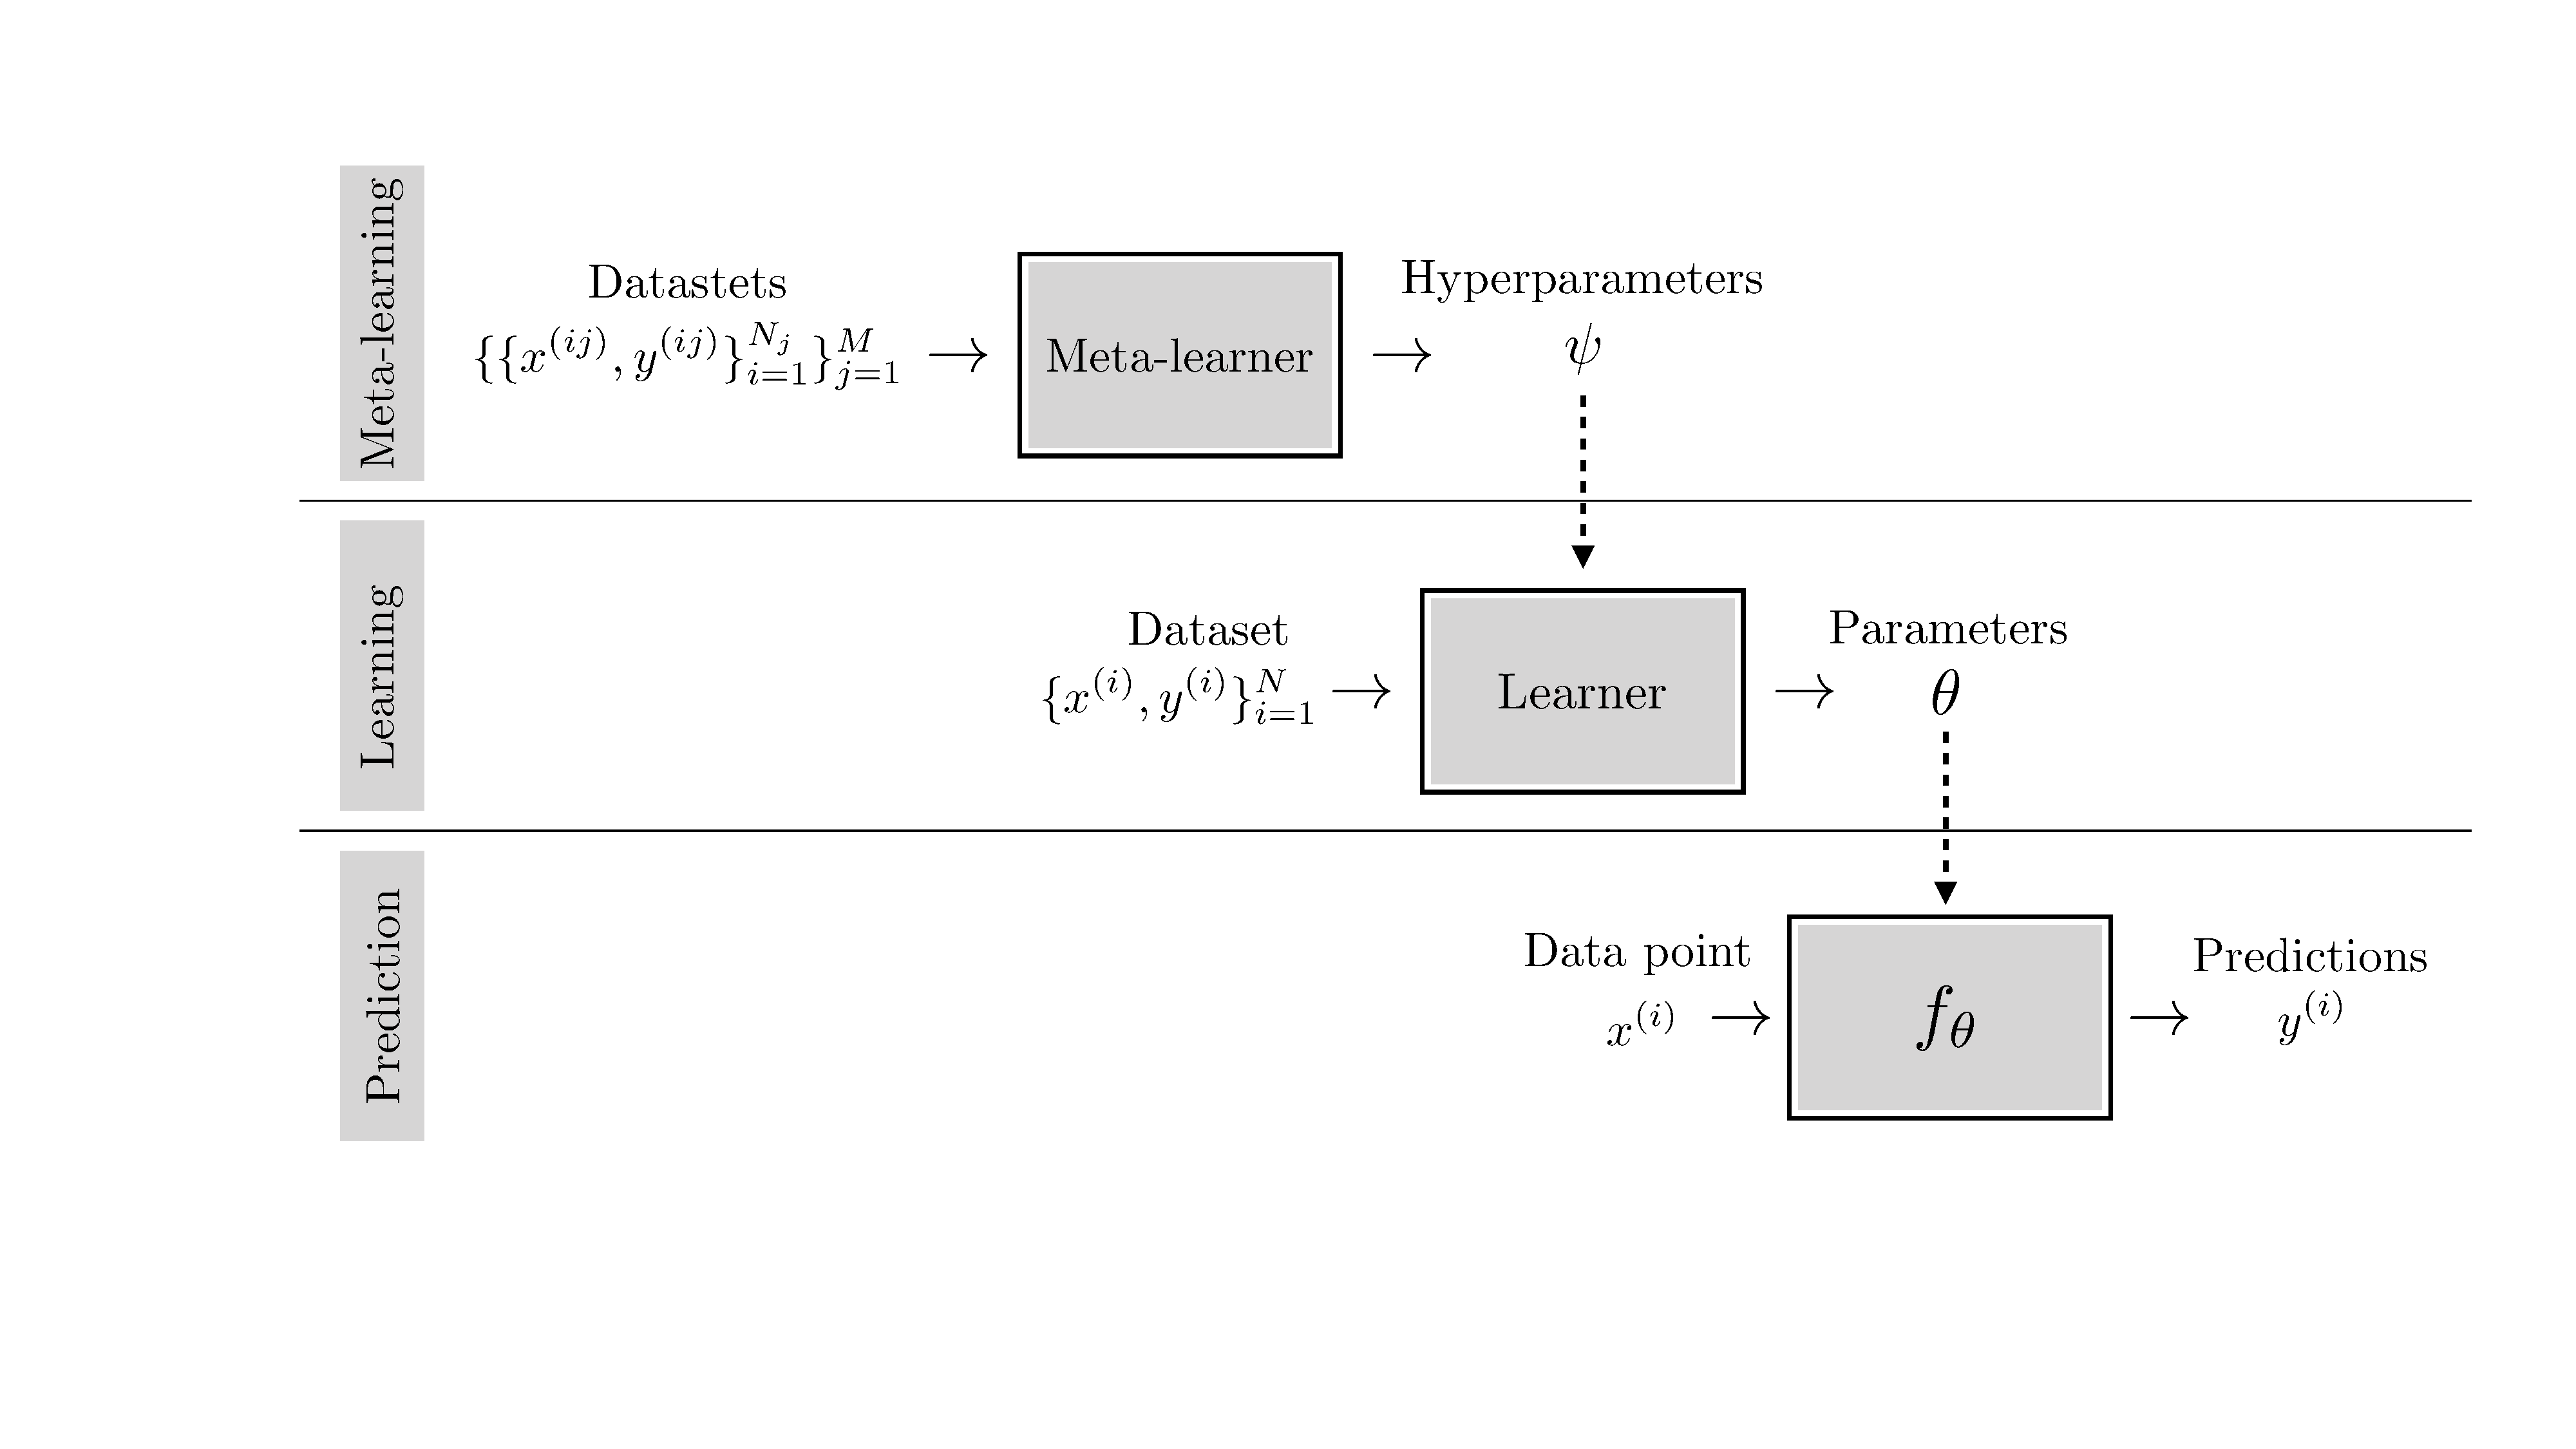
\includegraphics[width=1.0\linewidth]{./figures/intro_to_learning/meta_learning_diagram.pdf}
    }
    \caption{Learning is a meta-algorithm, an algorithm that outputs algorithms; metalearning is just learning applied to learning, and therefore it is a meta-meta-algorithm.}
    \label{fig:intro_to_learning:meta_learning_diagram}
\end{figure}

Notice that you can apply this idea recursively, constructing meta-meta-...-metalearners. Humans perform at least three levels of this process, if not more: we have \emph{evolved} to be \emph{taught} in school how to \emph{learn} quickly on our own.
\marginnote{{\bf Evolution} is a learning algorithm according to our present definition.}[-1.0cm]

\section{Concluding Remarks}
Learning is an extremely general and powerful approach to problem solving. It turns data into algorithms. In this era of big data, learning is very often the preferred approach. It is a a major component of almost all modern computer vision systems.
 % PHILLIP
% %\setcounter{chapter}{9}
\chapter{Gradient-Based Learning Algorithms}\label{chapter:gradient_descent}


\section{Introduction}

Once you have specified a learning problem (loss function, hypothesis space, parameterization), the next step is to find the parameters that minimize the loss. This is an optimization problem, and the most common optimization algorithm we will use is \index{Gradient descent}\textbf{gradient descent}. Gradient descent is like a skier making their way down a snowy mountain, where the shape of the mountain is the loss function.

There are many varieties of gradient descent, and we will call this whole family \textbf{gradient-based learning algorithms}. All share the same basic idea: at some operating point, calculate the direction of steepest descent, then use this direction to find a new operating point with lower loss.\marginnote{We use the term \textbf{operating point} to refer to a particular point (setting of the parameters) where we are currently evaluating the loss.}[-0.85cm]

\section{Technical Setting}
In this chapter, we consider the task of minimizing a cost function $J: \cdot \rightarrow \mathbb{R}$, which is a function that maps some arbitrary input to a scalar cost. %The domain of this function can be anything, but the range is always a scalar.

In learning problems, the domain of $J$ is the training data and the parameters $\theta$.\marginnote{Remember from \chap{\ref{chapter:intro_to_learning}} that in supervised learning, the training data is $\{\mathbf{x}^{(i)}, \mathbf{y}^{(i)}\}^N_{i=1}$, while in unsupervised learning the training data is $\{\mathbf{x}^{(i)}\}^N_{i=1}$.} Often, we will consider the training data to be fixed and only denote the objective as a function of the parameters, $J(\theta)$. Our goal is to solve:
\begin{align}
    \theta^* = \argmin_{\theta} J(\theta)
\end{align}

%When we evaluate $J$ at some specific location $\theta$, we will say that is the value of $J$ at operating point $\theta$. 

%$\nabla_{\theta} J \triangleq \frac{\partial J}{\partial \theta}$

Pretty much all optimizers work by some iterative process, where they update the parameters to be better and better. Different optimizers differ in how the parameter update function works. The update function gets to view some information about the loss landscape, then uses that information to update the parameters, as shown in \fig{\ref{fig:gradient_descent:optimization_schematic}}.
\begin{figure}[h]
    \centerline{
    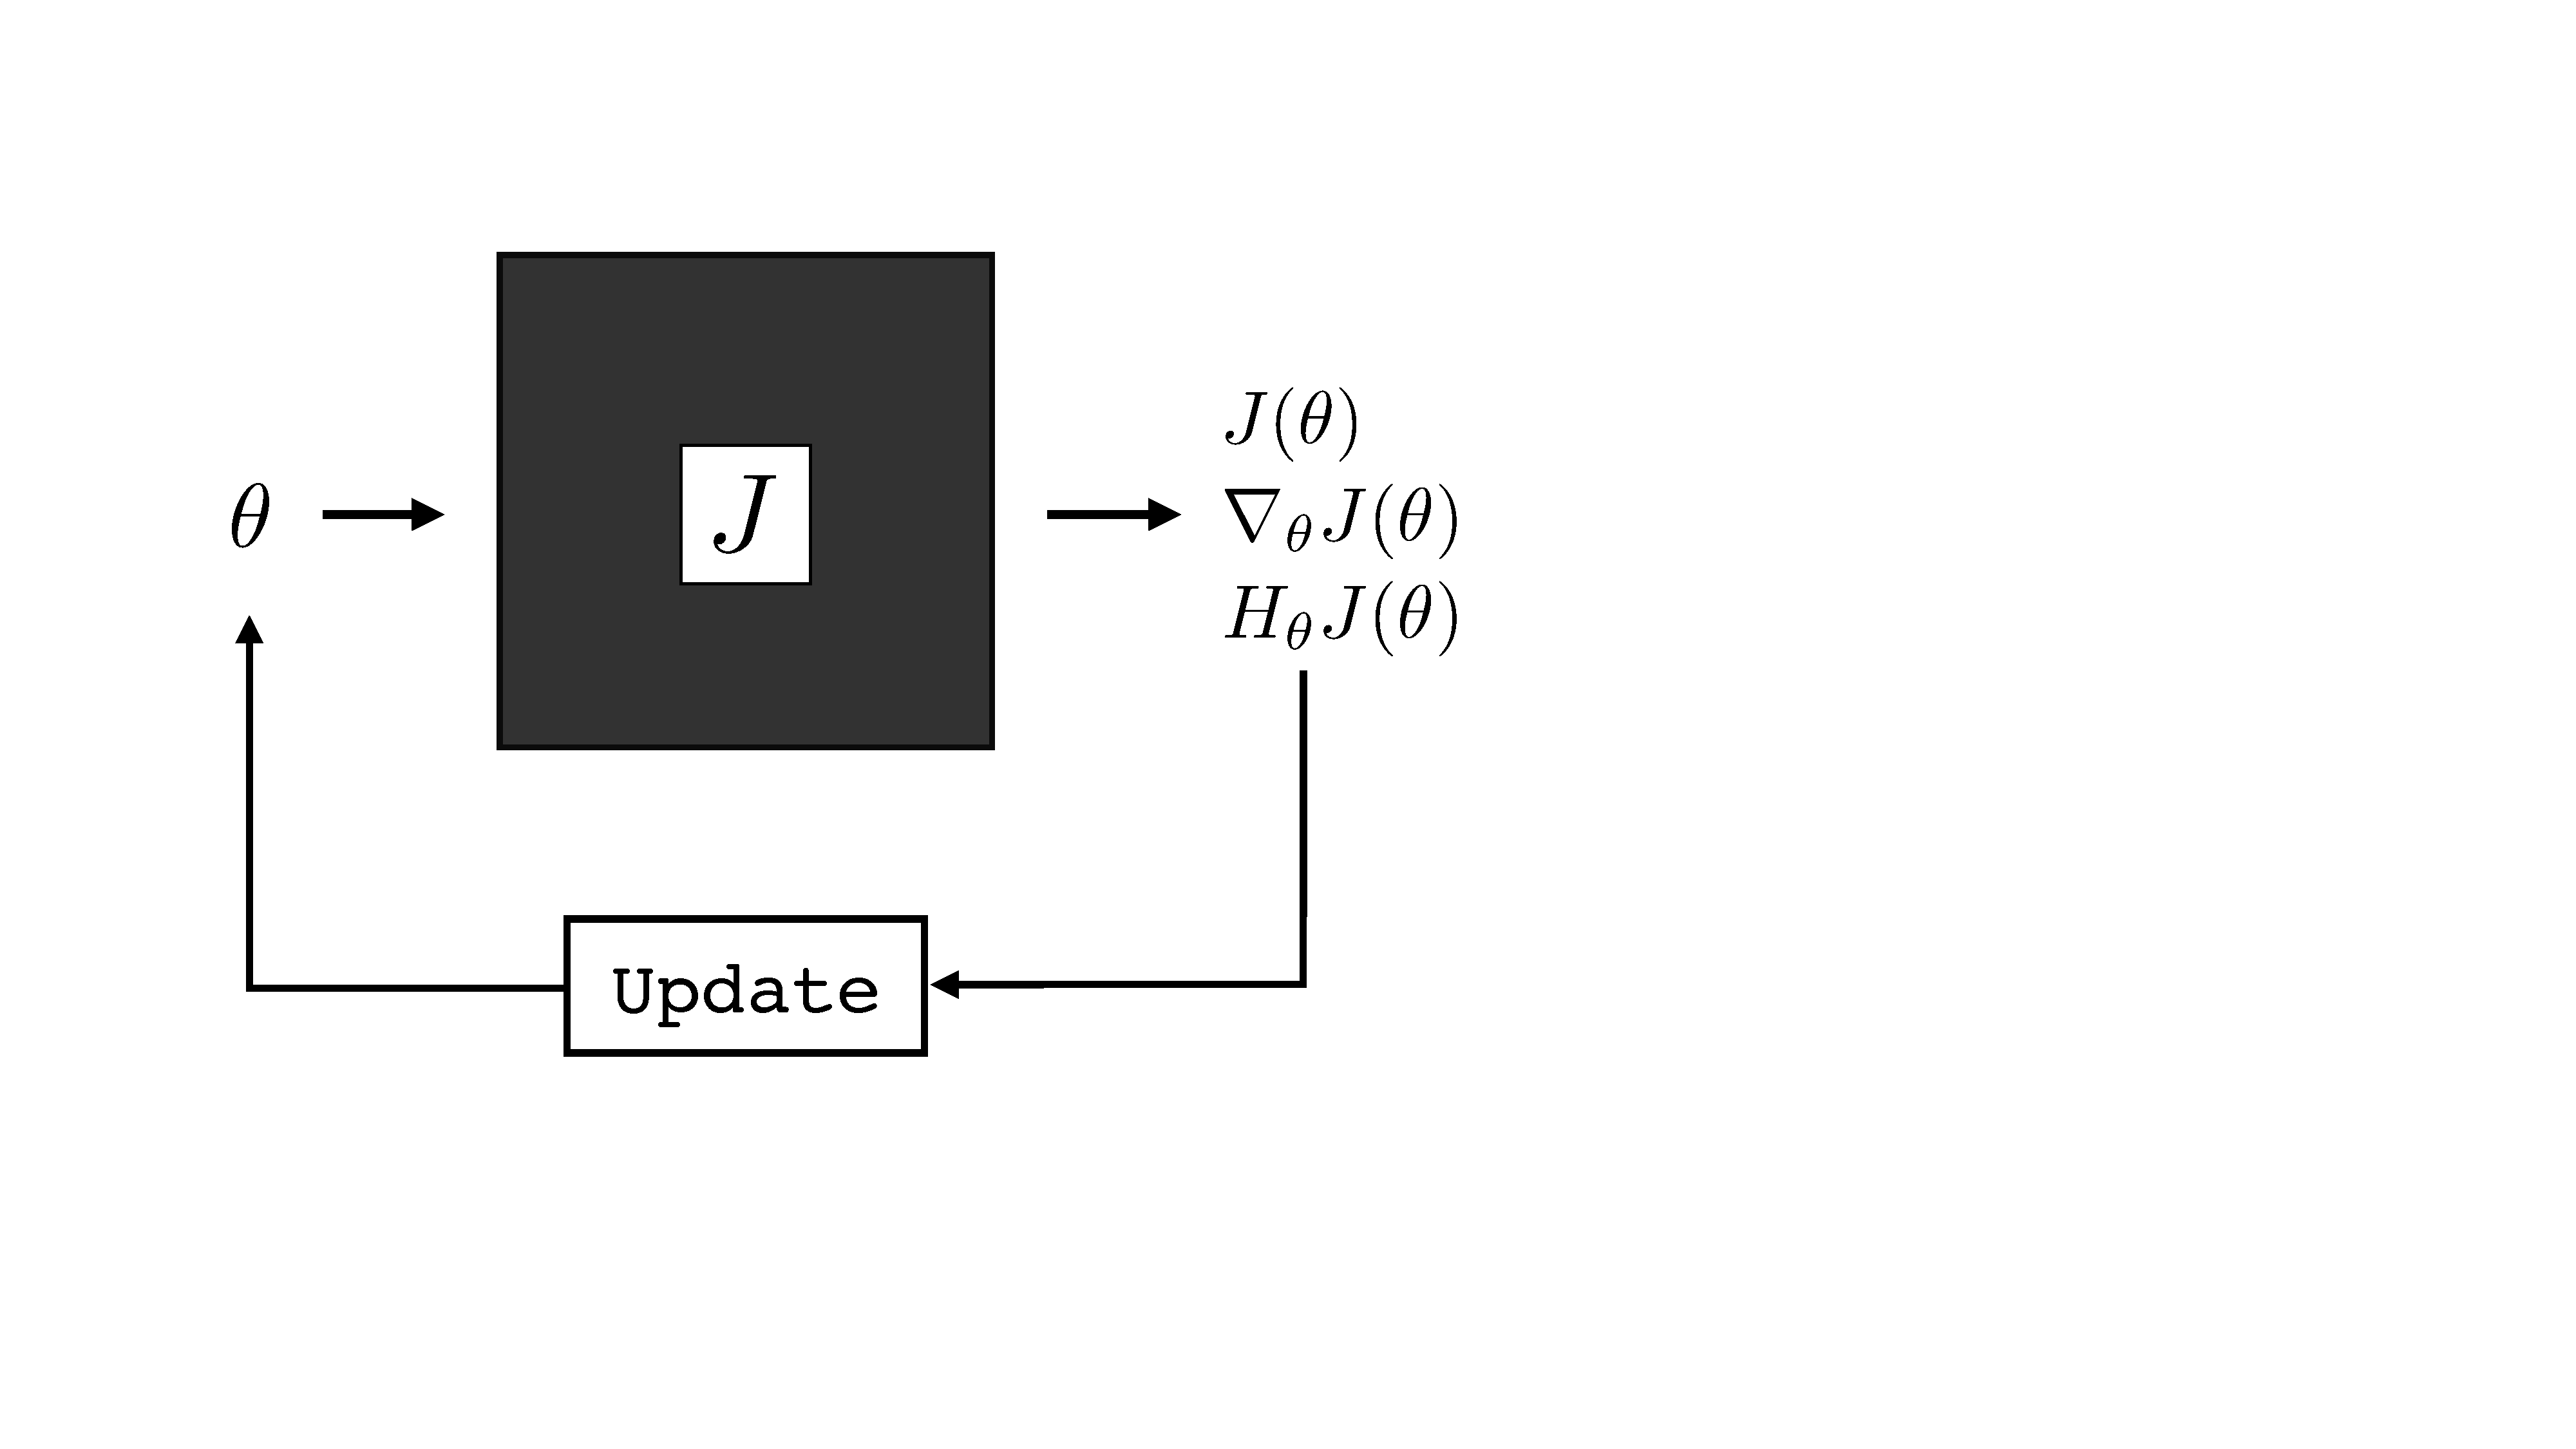
\includegraphics[width=0.35\linewidth]{./figures/gradient_descent/optimization_schematic.pdf}
    }
    \caption{General optimization loop.}
    \label{fig:gradient_descent:optimization_schematic}
\end{figure}

In the simplest setting, called \index{Zeroth-order optimization}\textbf{zeroth-order optimization}, the update function only gets to observe the value $J(\theta)$. The only way, then, to find $\theta$'s that minimize the loss is to sample different values for $\theta$ and move toward the values that are lower.

For gradient-based optimization, also called \index{First-order optimization}\textbf{first-order optimization}, the update function takes as input the gradient of the cost with respect to the parameters at the current operating point, $\nabla_{\theta}J(\theta)$. This reveals hugely useful information about the loss that directly tells us how to minimize it: just move in the direction of steepest descent, that is, the gradient direction.

Higher-order optimization methods observe higher-order derivatives of the loss, such as the Hessian $H$, which tells you how the landscape is locally curving. The Hessian is costly to compute but many methods use approximations to the Hessian, or other properties related to loss curvature, and these are growing in popularity~\cite{martens2015optimizing,foret2020sharpness}.


\section{Basic Gradient Descent}
The simplest version of gradient descent just takes a step in the gradient direction of length proportional to the gradient magnitude. This algorithm is described in \algref{\ref{alg:gradient_descent:basic_gradient_descent}}.
\begin{algorithm}[h]
\SetAlgoVlined
\DontPrintSemicolon
%\marginnote{{\bf Algorithm \ref{alg:gradient_descent:basic_gradient_descent}}: Optimizing a cost function $J: \theta \rightarrow \mathbb{R}$ by descending the gradient $\nabla_{\theta} J$.}
\caption{{\bf Algorithm \ref{alg:gradient_descent:basic_gradient_descent}}: Gradient descent (\texttt{GD}). Optimizing a cost function $J: \theta \rightarrow \mathbb{R}$ by descending the gradient $\nabla_{\theta} J$.}
\fakealgorithmcaption{}
\label{alg:gradient_descent:basic_gradient_descent}
{\bf Input:} objective function $J$, initial parameter vector $\theta^0$, learning rate $\eta$, number of steps $K$\;%, data $\{\mathbf{x}^{(i)},\mathbf{y}^{(i)}\}_{i=1}^N$
{\bf Output:} trained parameter vector $\theta^* = \theta^K$\;
\For{\upshape $k= 0, \dots, K-1$}{
    %$J = \sum_{i=1}^N \mathcal{L}(f_{\theta^{k}}(\mathbf{x}^{(i)}),\mathbf{y}^{(i)})$\;
    $\theta^{k+1} \leftarrow \theta^{k} - \eta \nabla_{\theta} J(\theta^k)$\;
}
\end{algorithm}

This algorithm has two hyperparameters, the \index{Learning rate}\textbf{learning rate} $\eta$, which controls the step size (learning rate times gradient magnitude), and the number of steps $K$. If the learning rate is sufficiently small and the initial parameter vector $\theta^0$ is random, then this algorithm will almost surely converge to a local minimum of $J$ as $K \rightarrow \infty$~\cite{lee2016gradient}. However, to descend more quickly, it can be useful to set the learning rate to a higher value. 

\section{Learning Rate Schedules}
A generally useful strategy is to start with a high value for $\eta$ and then decay it until convergence according to a \textbf{learning rate schedule}. Researchers have come up with innumerable schedules and they generally work by calling some function $\texttt{lr}(\eta^0,k)$ to get the learning rate on each iteration of descent:
\begin{align}
    \eta^{k} = \texttt{lr}(\eta^0,k)
\end{align}
Generally, we want an update rule where $\eta^{k+1} < \eta^k$, so that we take smaller steps as we approach the minimizer. A few simple and popular approaches are given below:
\begin{align}
    \texttt{lr}(\eta^0,k) &= \beta^{-k} \eta^0 &\quad\quad \triangleleft\quad \text{exponential decay}\\
    \texttt{lr}(\eta^0,k) &= \beta^{-\lfloor k/M \rfloor} \eta^0 &\quad\quad \triangleleft\quad \text{stepwise exponential decay}\\
    \texttt{lr}(\eta^0,k) &= \frac{(K - k)}{K} \eta^0 &\quad\quad \triangleleft\quad \text{linear decay}
\end{align}
\marginnote{One downside of linear decay is that it depends on the total number of steps $K$. This makes it hard to compare optimization runs of different lengths. This is something to also be aware of in more advanced learning rate schedules, such as cosine decay~\cite{loshchilov2016sgdr}, which also have different behavior for different settings of $K$.}[-3.2cm]
The $\beta$ and $M$ are additional hyperparameters of these methods. The general approach of learning rate decay is summarized in \algref{\ref{alg:gradient_descent:gradient_descent_with_lr_decay}}.

%but a simple one that tends to work decently is to just multiply the $\eta$ by a  constant factor $\beta \in (0,1)$ every iteration of gradient descent, where $\beta$ and the initial learning rate $\eta^1$ are the new hyperparameters to specify. 
\begin{algorithm}[h]
\SetAlgoVlined
\DontPrintSemicolon
%\marginnote{{\bf Algorithm \ref{alg:gradient_descent:gradient_descent_with_lr_decay}}: Gradient descent with a learning rate schedule.}
\caption{{\bf Algorithm \ref{alg:gradient_descent:gradient_descent_with_lr_decay}}: Gradient descent with a learning rate schedule.}
%\caption{{\bf Algorithm \ref{alg:gradient_descent:gradient_descent_with_lr_decay}}: \texttt{GD}+\texttt{lr}-schedule.}
\fakealgorithmcaption{}
\label{alg:gradient_descent:gradient_descent_with_lr_decay}
{\bf Input:} objective function $J$, initial parameter vector $\theta^0$, initial learning rate $\eta^0$, learning rate function $\texttt{lr}$, number of steps $K$\;%, data $\{\mathbf{x}^{(i)},\mathbf{y}^{(i)}\}_{i=1}^N$
{\bf Output:} trained parameter vector $\theta^* = \theta^K$\;
\For{\upshape $k= 0, \dots, K-1$}{
    %$J = \sum_{i=1}^N \mathcal{L}(f_{\theta^{k-1}}(\mathbf{x}^{(i)}),\mathbf{y}^{(i)})$\;
    $\eta^{k} \leftarrow \texttt{lr}(\eta^0, k)$\;
    $\theta^{k+1} \leftarrow \theta^{k} - \eta^{k} \nabla_{\theta} J(\theta^k)$\;
}
\end{algorithm}

Variations on this algorithm include only decaying the learning rate when a plateau is reached (i.e., when the loss is not decreasing for many iterations in a row), or decaying the learning rate according to more complex nonlinear schedules, such as one shaped like a cosine function~\cite{loshchilov2016sgdr}.%once every $M$ steps of gradient descent, for some fixed value $M$ (which becomes an additional hyperparameter of the algorithm).

\section{Momentum}
Could we do a smarter update than just taking a step in the direction of the gradient? Of the countless ideas that have been proposed, one of the few that has stuck is \index{Momentum}\textbf{momentum}~\cite{polyak1964some,sutskever2013importance}. Momentum makes the analogy to skiing even more precise: momentum is like the inertia of the skier, carrying them over the little bumps and imperfections in the ski slope and increasing their speed as they descend along a straight path. In math, momentum just means that we set the parameter update to be a direction $\mathbf{v}^{k+1}$, given by a weighted combination of the previous update direction, $\mathbf{v}^{k}$, plus the current negative gradient:
\begin{align}
    \mathbf{v}^{k+1} = \mu \mathbf{v}^{k} - \eta\nabla_{\theta} J(\theta^k)
\end{align}
The weight $\mu$ in this combination is a new hyperparameter, sometimes simply called the momentum. The full algorithm is given in \algref{\ref{alg:gradient_descent:gradient_descent_with_momentum}}.
\begin{algorithm}[h]
\SetAlgoVlined
\DontPrintSemicolon
%\marginnote{{\bf Algorithm \ref{alg:gradient_descent:gradient_descent_with_momentum}}: Gradient descent with momentum.}
\caption{{\bf Algorithm \ref{alg:gradient_descent:gradient_descent_with_momentum}}: Gradient descent with momentum.}
\fakealgorithmcaption{}
\label{alg:gradient_descent:gradient_descent_with_momentum}
{\bf Input:} objective function $J$, initial parameter vector $\theta^0$, learning rate $\eta$, momentum $\mu$, number of steps $K$\;%, data $\{\mathbf{x}^{(i)},\mathbf{y}^{(i)}\}_{i=1}^N$
{\bf Output:} trained parameter vector $\theta^* = \theta^K$\;
$\mathbf{v}^{0} = \mathbf{0}$\;
\For{\upshape $k= 0, \dots, K-1$}{
    $\mathbf{v}^{k+1} = \mu \mathbf{v}^{k} - \eta\nabla_{\theta} J(\theta^k)$\;
    $\theta^{k+1} \leftarrow \theta^{k} + \mathbf{v}^{k+1}$\;
}
\end{algorithm}

\Fig{\ref{fig:gradient_descent:momentum_out1}} shows how momentum affects gradient descent for a simple objective $J = \texttt{abs}(\theta)$ (absolute value of $\theta$). As can be seen in the figure, some momentum can help convergence rate (\fig{\ref{fig:gradient_descent:momentum_out1}}, $\mu = 0.5$) but too much momentum will cause the trajectory to overshoot the optimum and even when the optimum loss is achieved, the trajectory might not stop (\fig{\ref{fig:gradient_descent:momentum_out1}}, $\mu = 0.95$).

\begin{figure}[h]
    \centering
    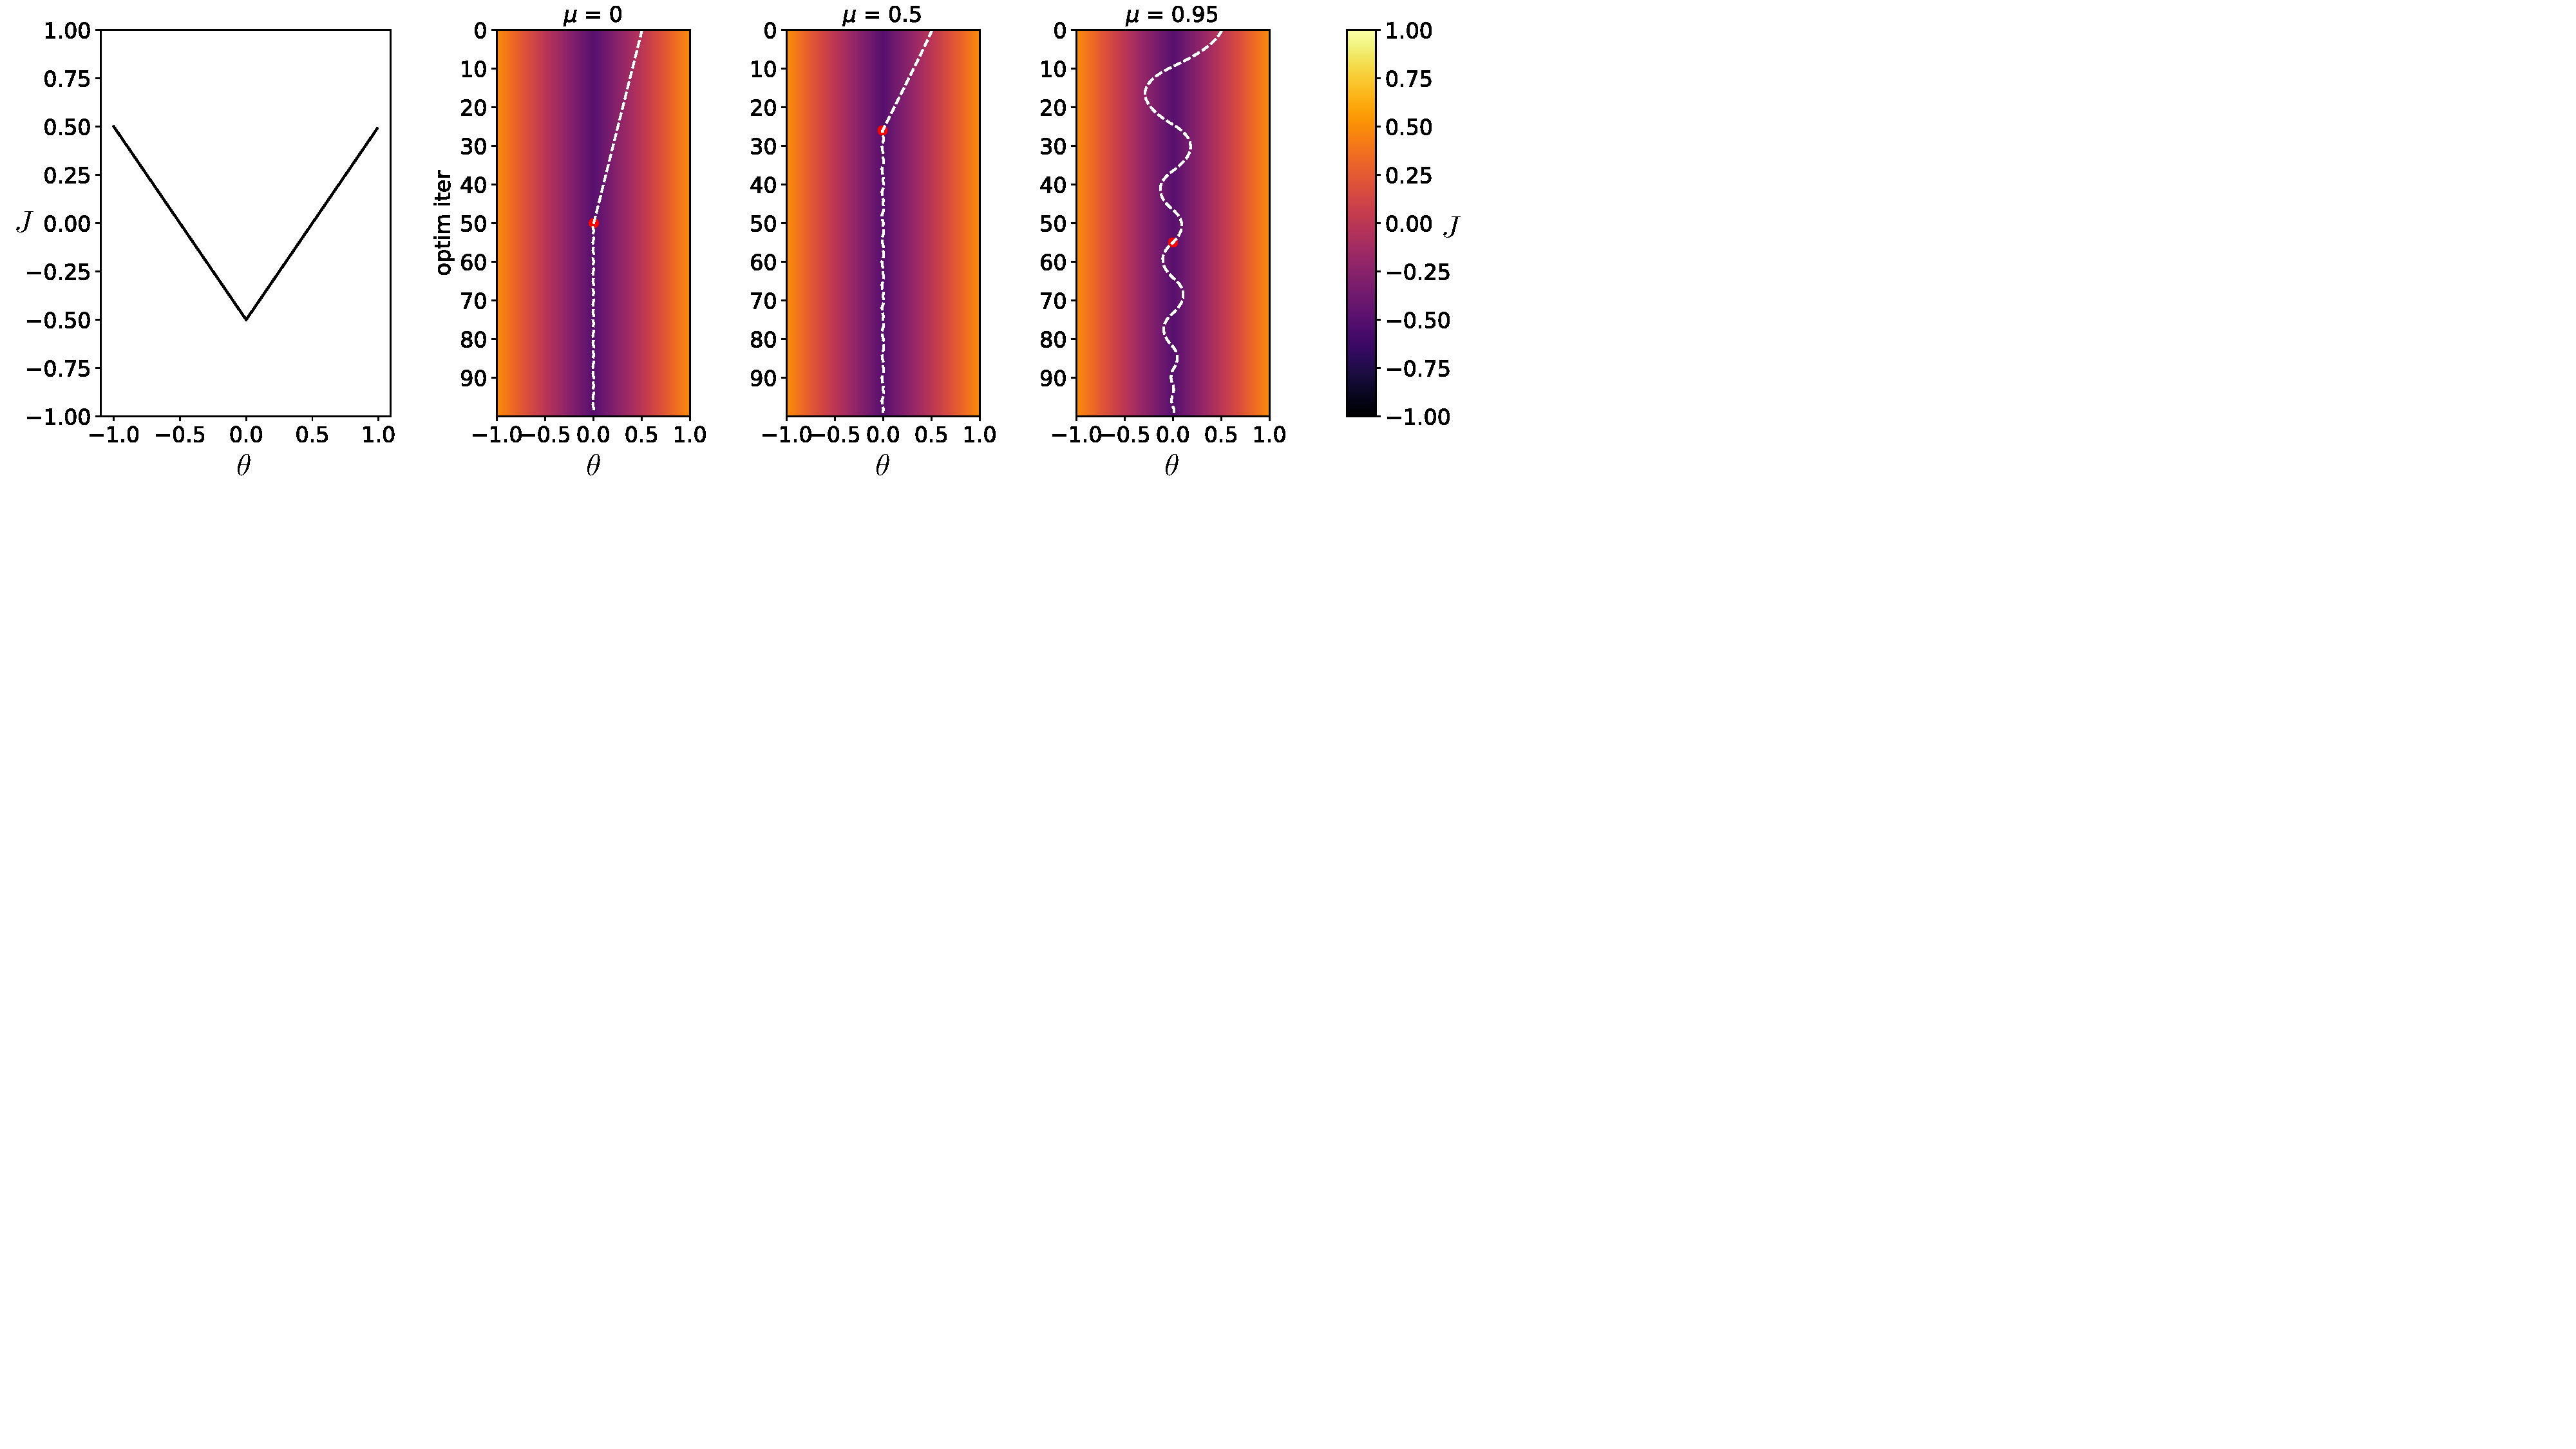
\includegraphics[width=1.0\linewidth]{./figures/gradient_descent/momentum_out1.pdf}
    \caption{(left) A simple loss function $J = \texttt{abs}(\theta)$. (right) Optimization trajectory for three different settings of momentum $\mu$. White line indicates value of the parameter at each iteration of optimization, starting at top and progressing to bottom. Color is value of the loss. Red dot is location where loss first reaches within $0.01$ of optimal value.}
    \label{fig:gradient_descent:momentum_out1}
\end{figure}

It is also possible to come up with other kinds of momentum, which bias the update direction based on some accumulated information from previous updates. Two popular alternatives, which you can read up on elsewhere, are Nesterov's accelerated gradient~\cite{nesterov1983method} and Adam~\cite{kingma2014adam}.


\section{What Kinds of Functions Can Be Minimized with Gradient Descent?}

What if a function is not differentiable? Can we still use gradient descent? Sometimes! The property we need is that we can get a meaningful signal as to how to perturb the function's parameters in order to reduce the loss. This property is \textit{not} the same as differentiability defined in math textbooks. A function may be differentiable but not give useful gradients (e.g., if the gradient is zero everywhere), and a function may be nondifferentiable (at certain points) but still allow for meaningful gradient-based updates (e.g., \texttt{abs}).

\Fig{\ref{fig:gradient_descent:grad_descent_simple_examples}} gives examples of different types of functions being minimized with gradient descent. \Figs{\ref{fig:gradient_descent:grad_descent_simple_examples}}(b) and \ref{fig:gradient_descent:grad_descent_simple_examples}(d) are cases where the function is discontinuous, and the analytical derivative is undefined at the discontinuity. Surprisingly, in \fig{\ref{fig:gradient_descent:grad_descent_simple_examples}}(b), this is not a problem for gradient descent. This is because the gradient descent algorithm we are using here (the one used by Pytorch~\cite{paszke2019pytorch}) uses a \index{One-sided derivative}\textbf{one-sided derivative} at the discontinuity, that is, we set the gradient at the discontinuity to be equal to the gradient value an infinitesimal step away from the discontinuouity in a fixed arbitrary direction. Under the hood, for each atomic discontinuous operation, Pytorch requires that we define its gradients at the discontinuouities, and the one-sided gradient is a standard choice. This is why it can be fine in deep learning (\chap{\ref{chapter:neural_nets}}) to use functions like rectified nonlinear units (relus), which are common in deep networks and have discontinuous gradients.

\Figs{\ref{fig:gradient_descent:grad_descent_simple_examples}}(c) and (e) give cases where the function is continuous, but the gradients are not well-behaved. In \fig{\ref{fig:gradient_descent:grad_descent_simple_examples}}(c) we have a gradient that has nearly \index{Vanishing gradient}\textbf{vanished}, that is, it is near zero everywhere and gradient descent, with a fixed learning rate, will therefore be slow. \Fig{\ref{fig:gradient_descent:grad_descent_simple_examples}}(e) shows the opposite scenario: the gradient at the minimizer goes to infinity; we call this an \index{Exploding gradient}\textbf{exploding gradient}, and this leads to failures of convergence. 

Finally, \fig{\ref{fig:gradient_descent:grad_descent_simple_examples}}(f) shows one more problematic case: when there are multiple minima, gradient descent can get stuck in a suboptimal minimum. Which minimum we arrive at will depend on where we initialized $x$.  

\begin{figure}[h!]
    \centerline{
    \begin{tabular}{cc}
        (a) convex & (b) discontinuous \\
        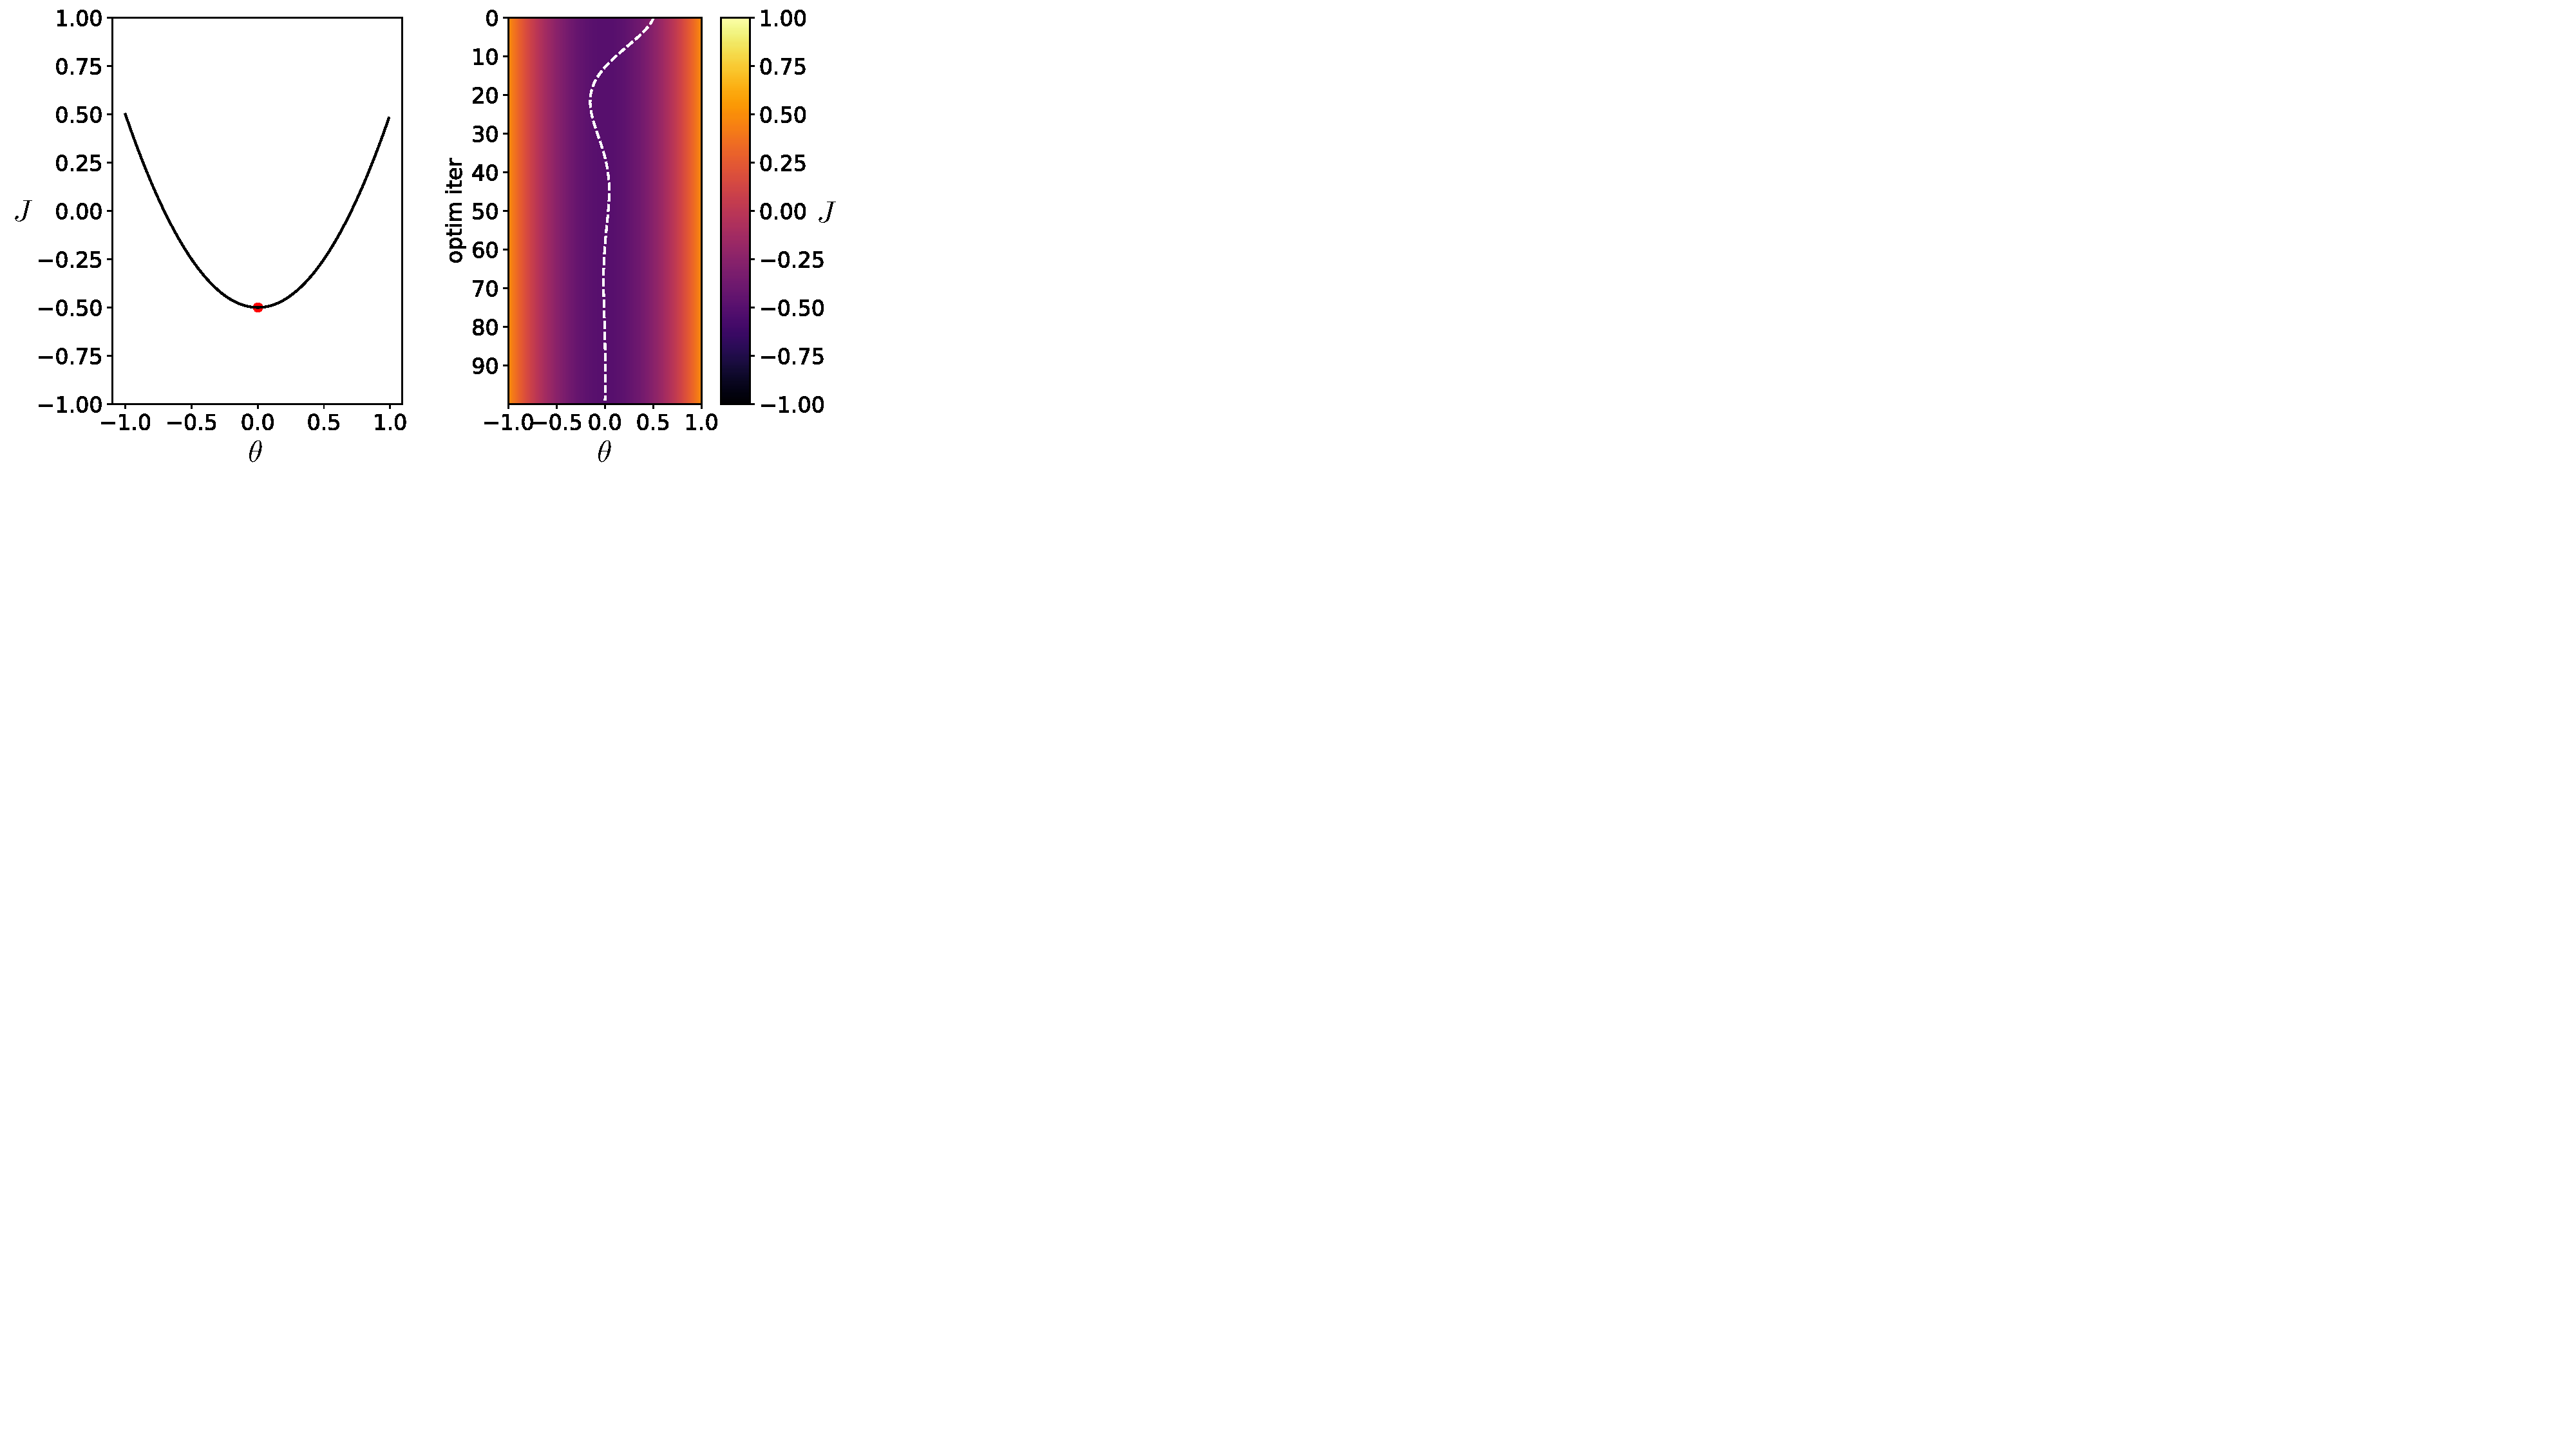
\includegraphics[width=0.5\linewidth]{./figures/gradient_descent/grad_descent_ex1.pdf} & 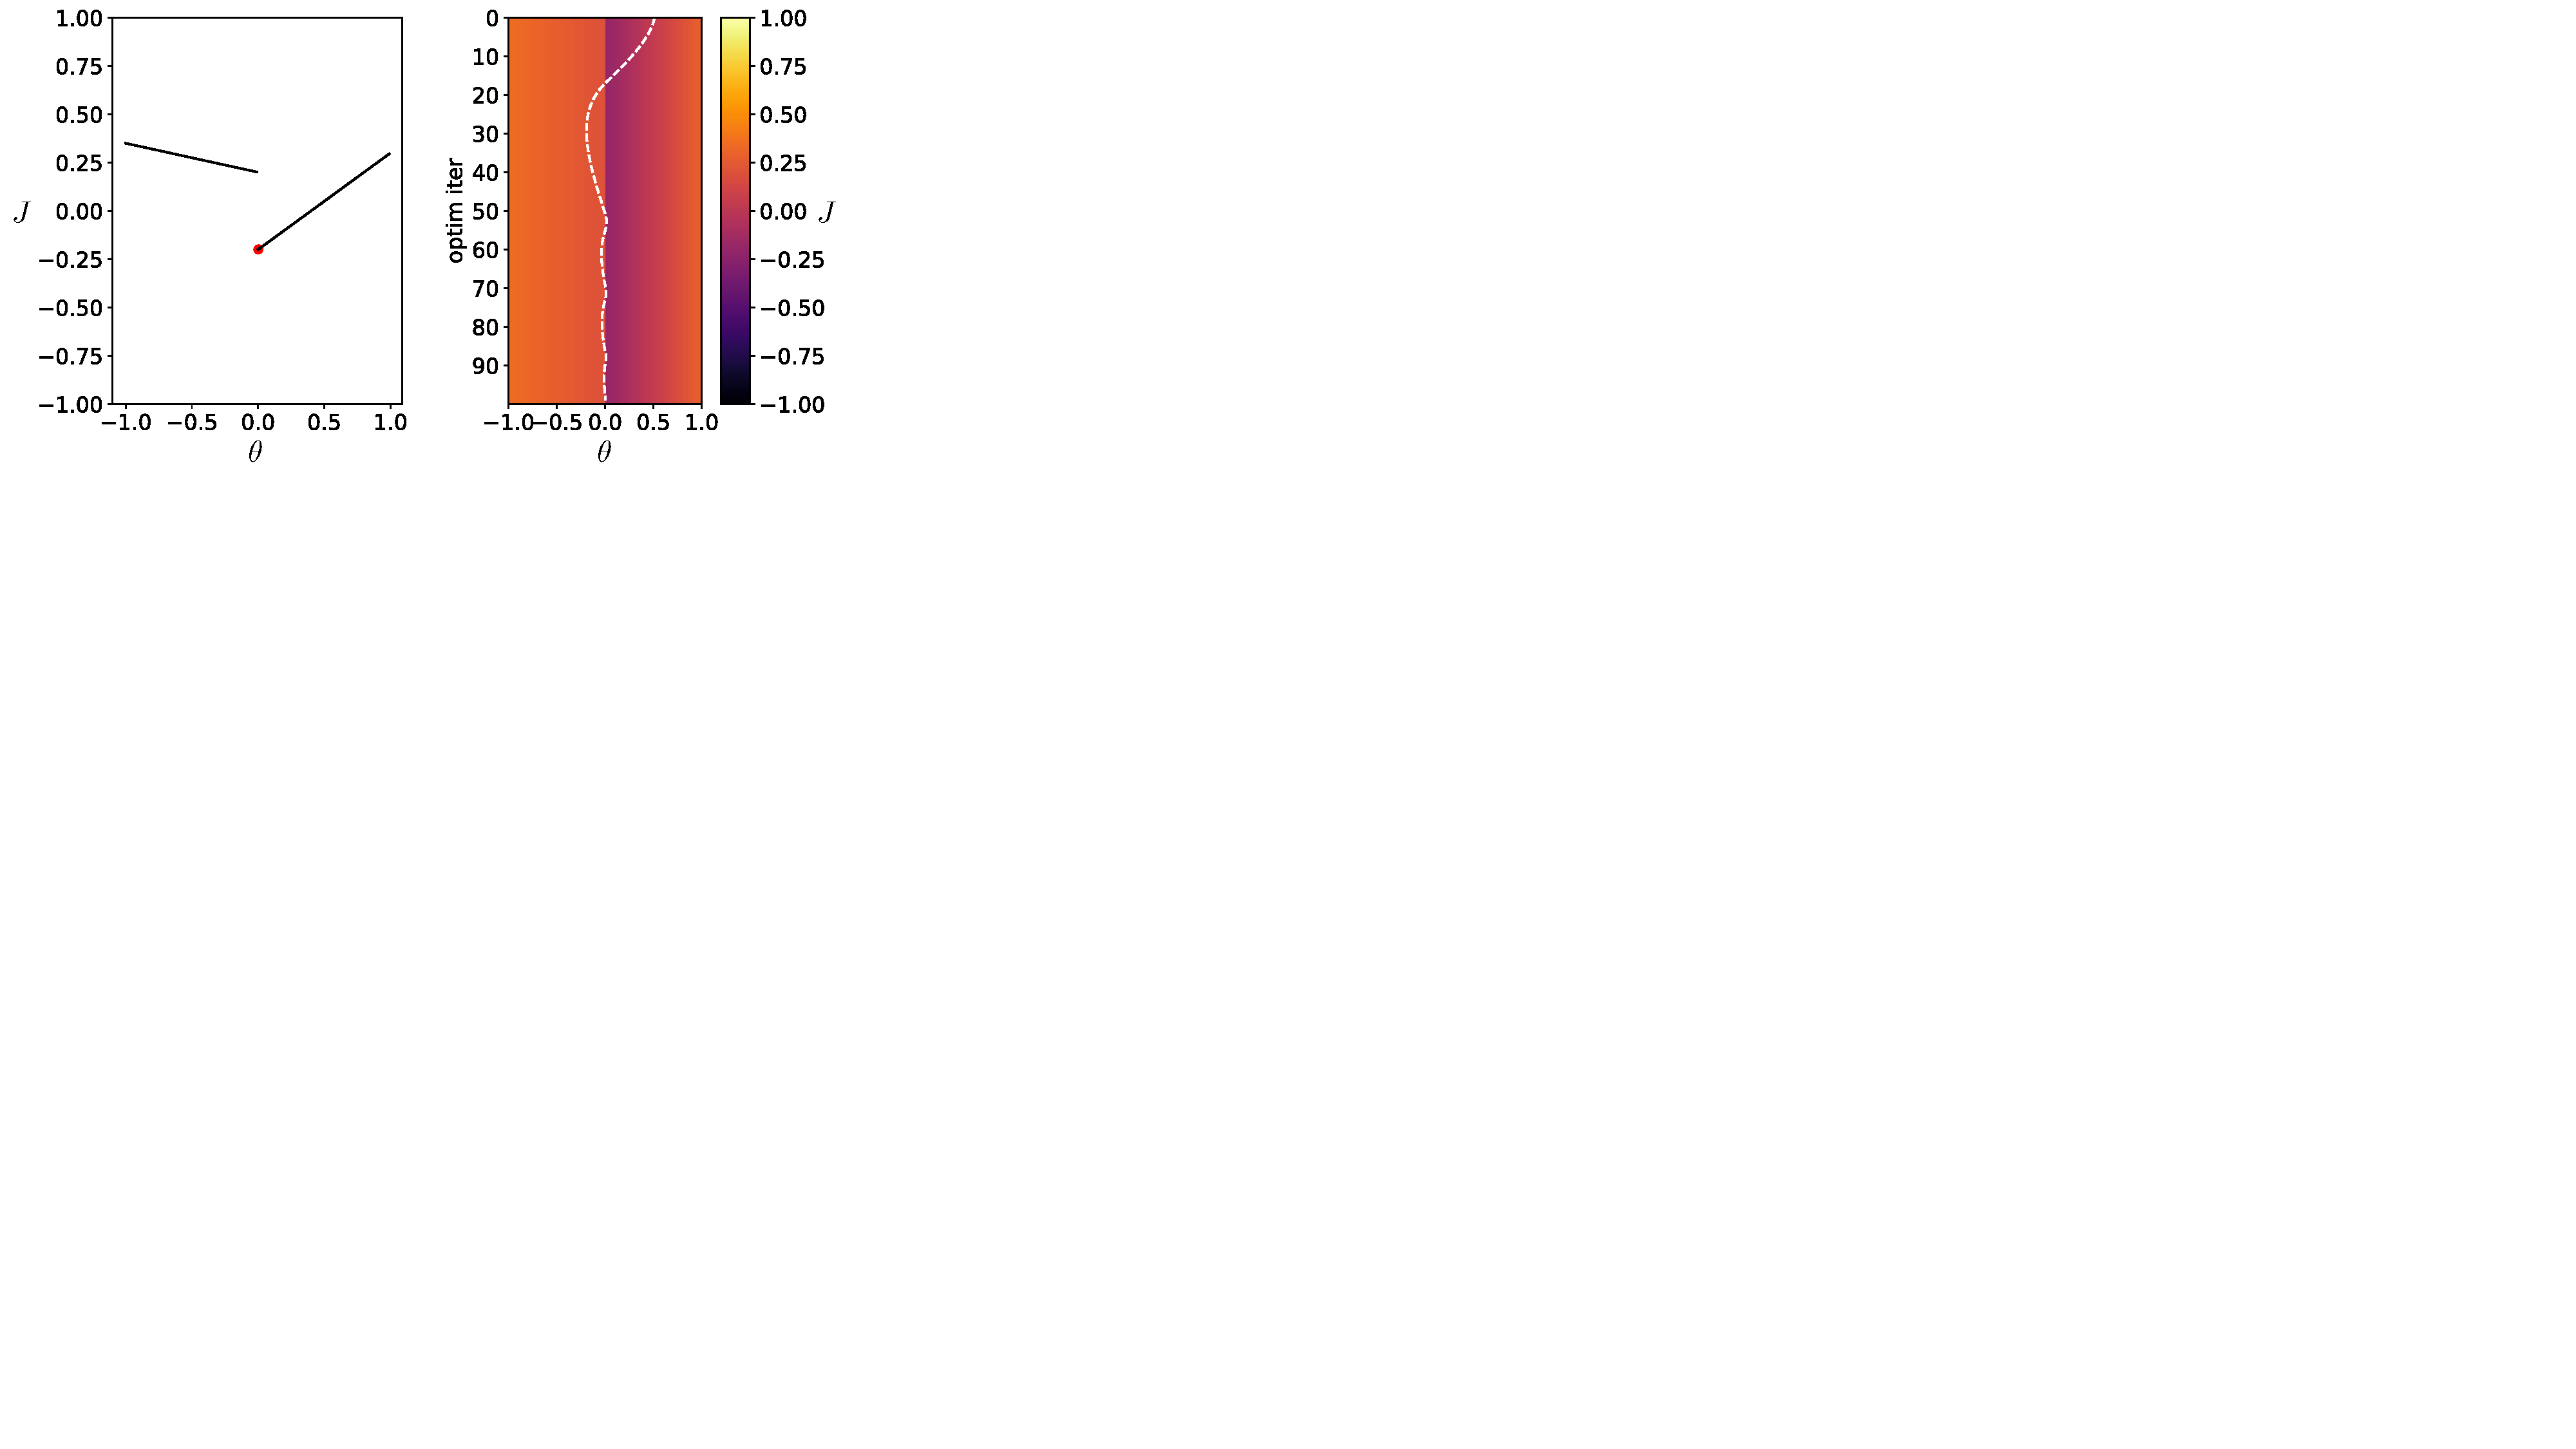
\includegraphics[width=0.5\linewidth]{./figures/gradient_descent/grad_descent_ex2.pdf} \\
        (c) vanishing gradient & (d) zero gradient + discontinuous \\
        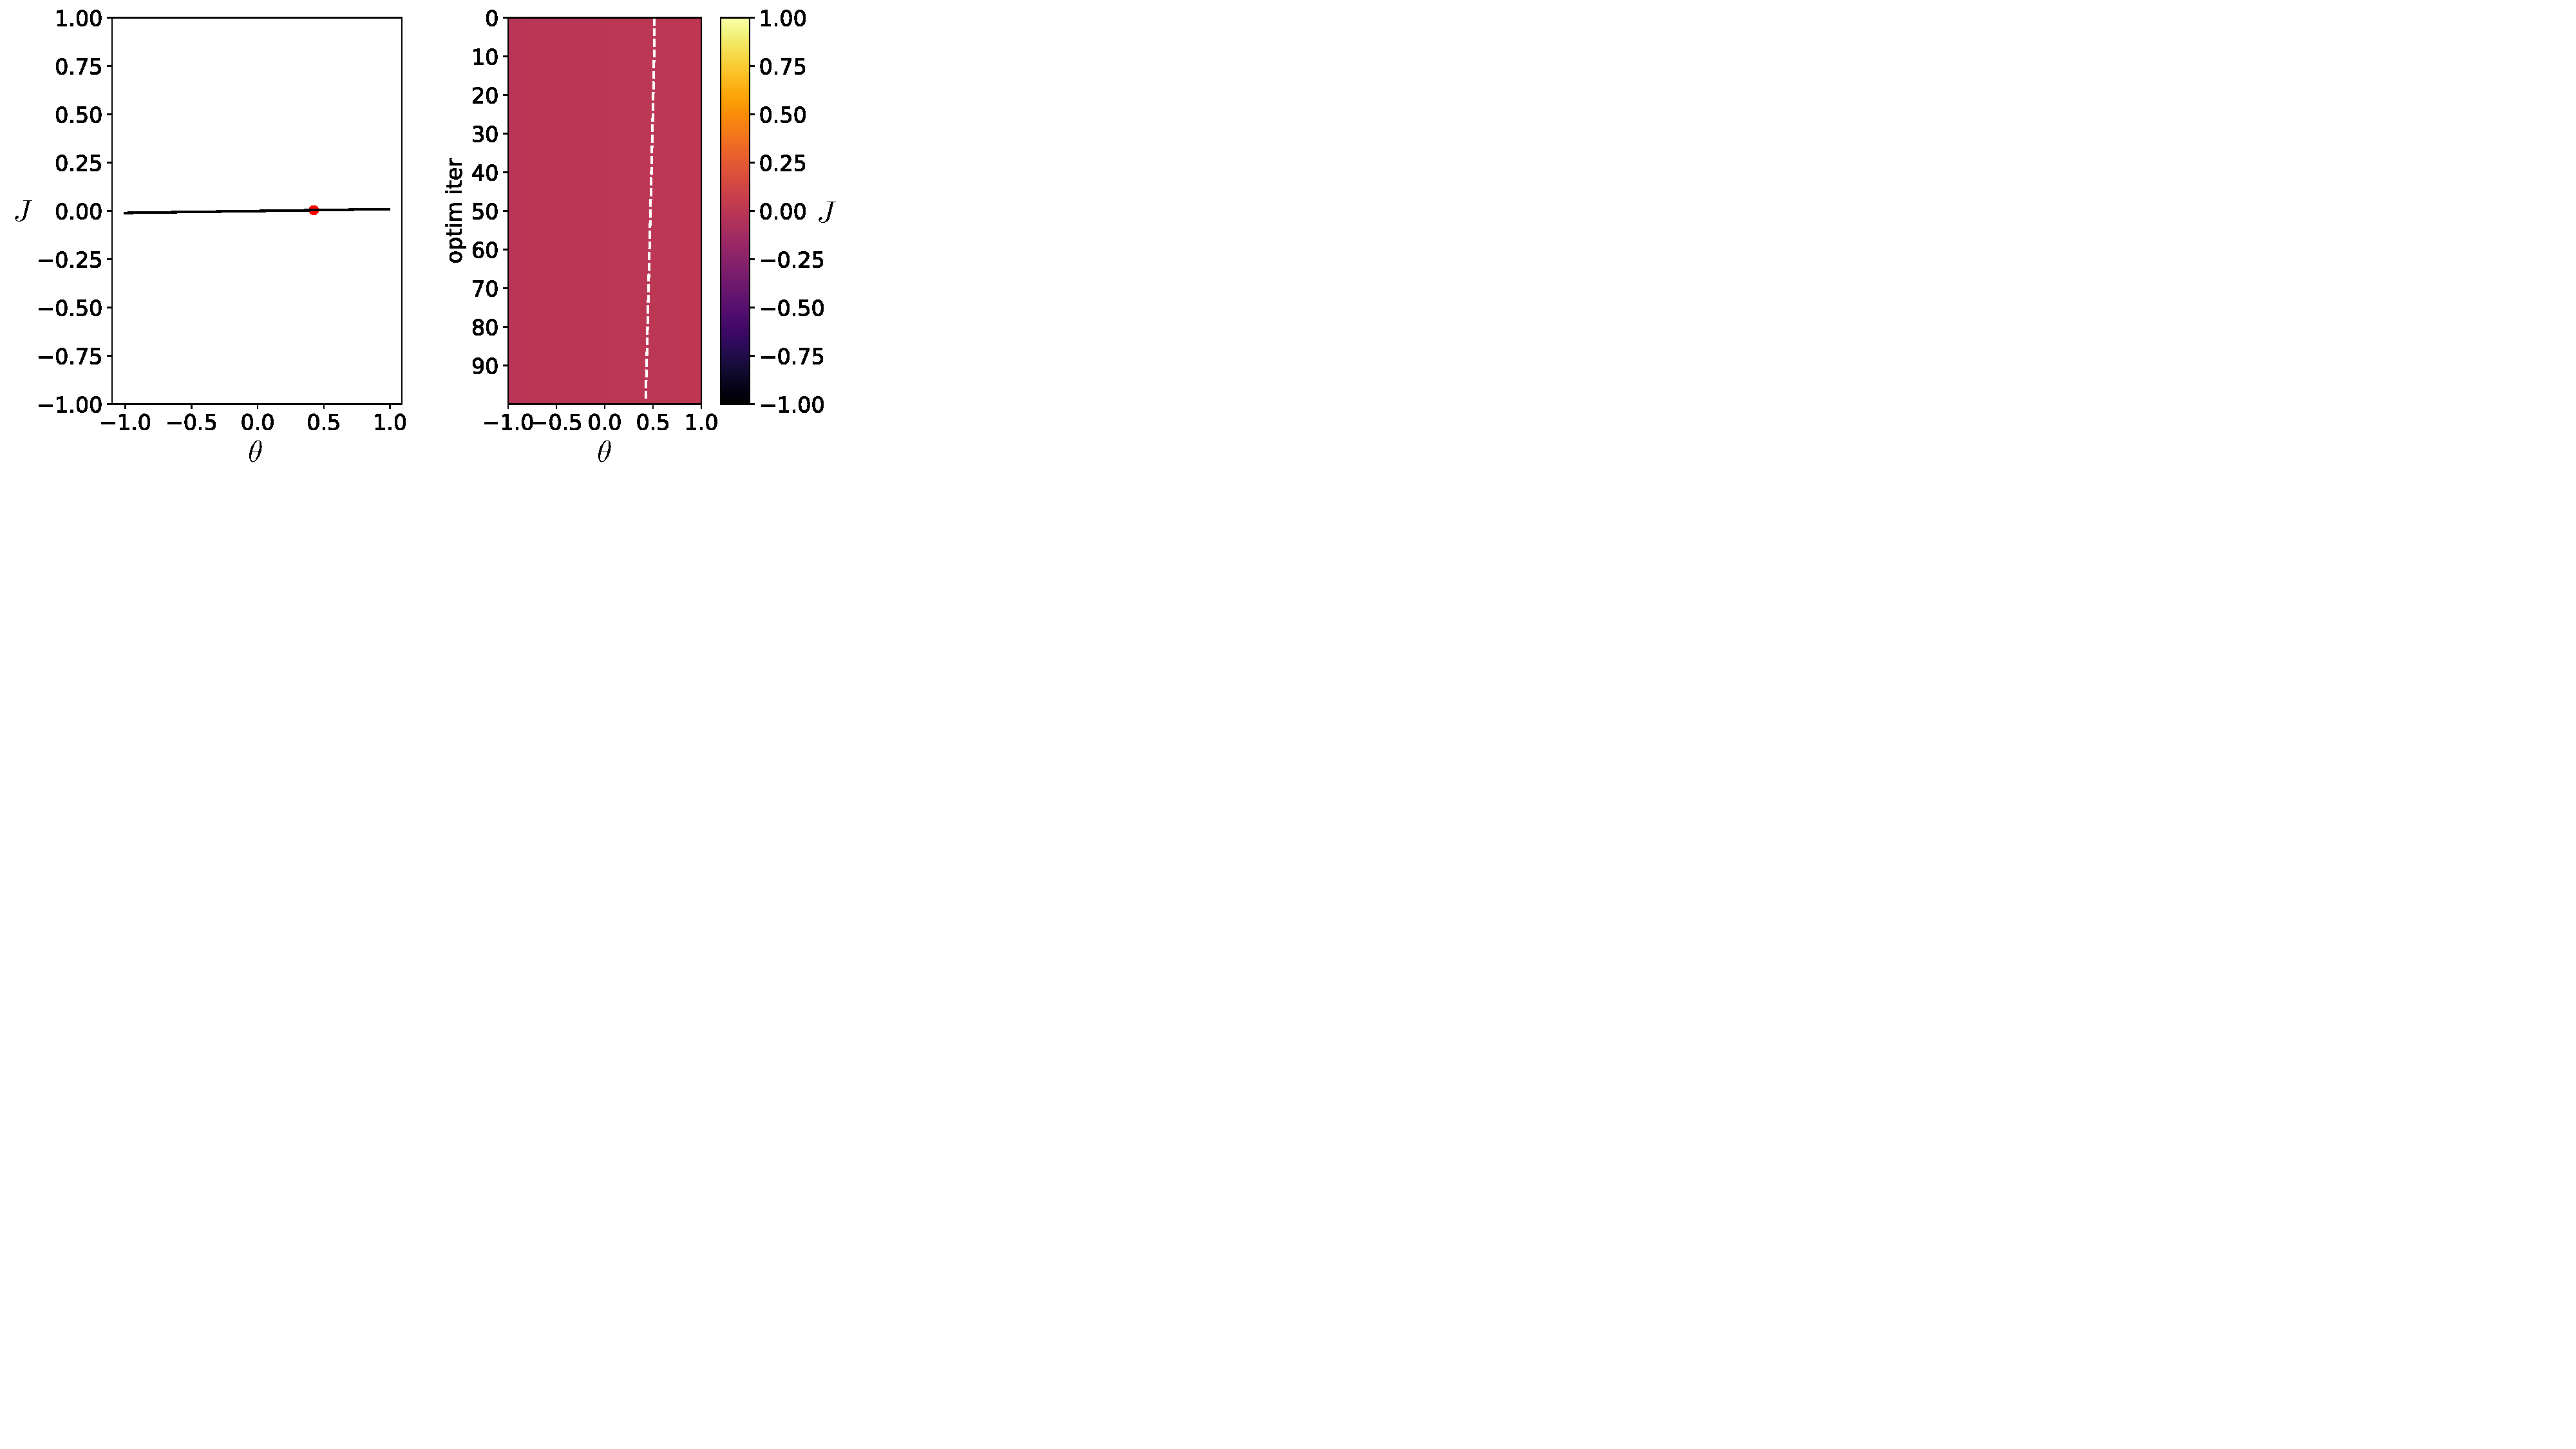
\includegraphics[width=0.5\linewidth]{./figures/gradient_descent/grad_descent_ex4.pdf} &
        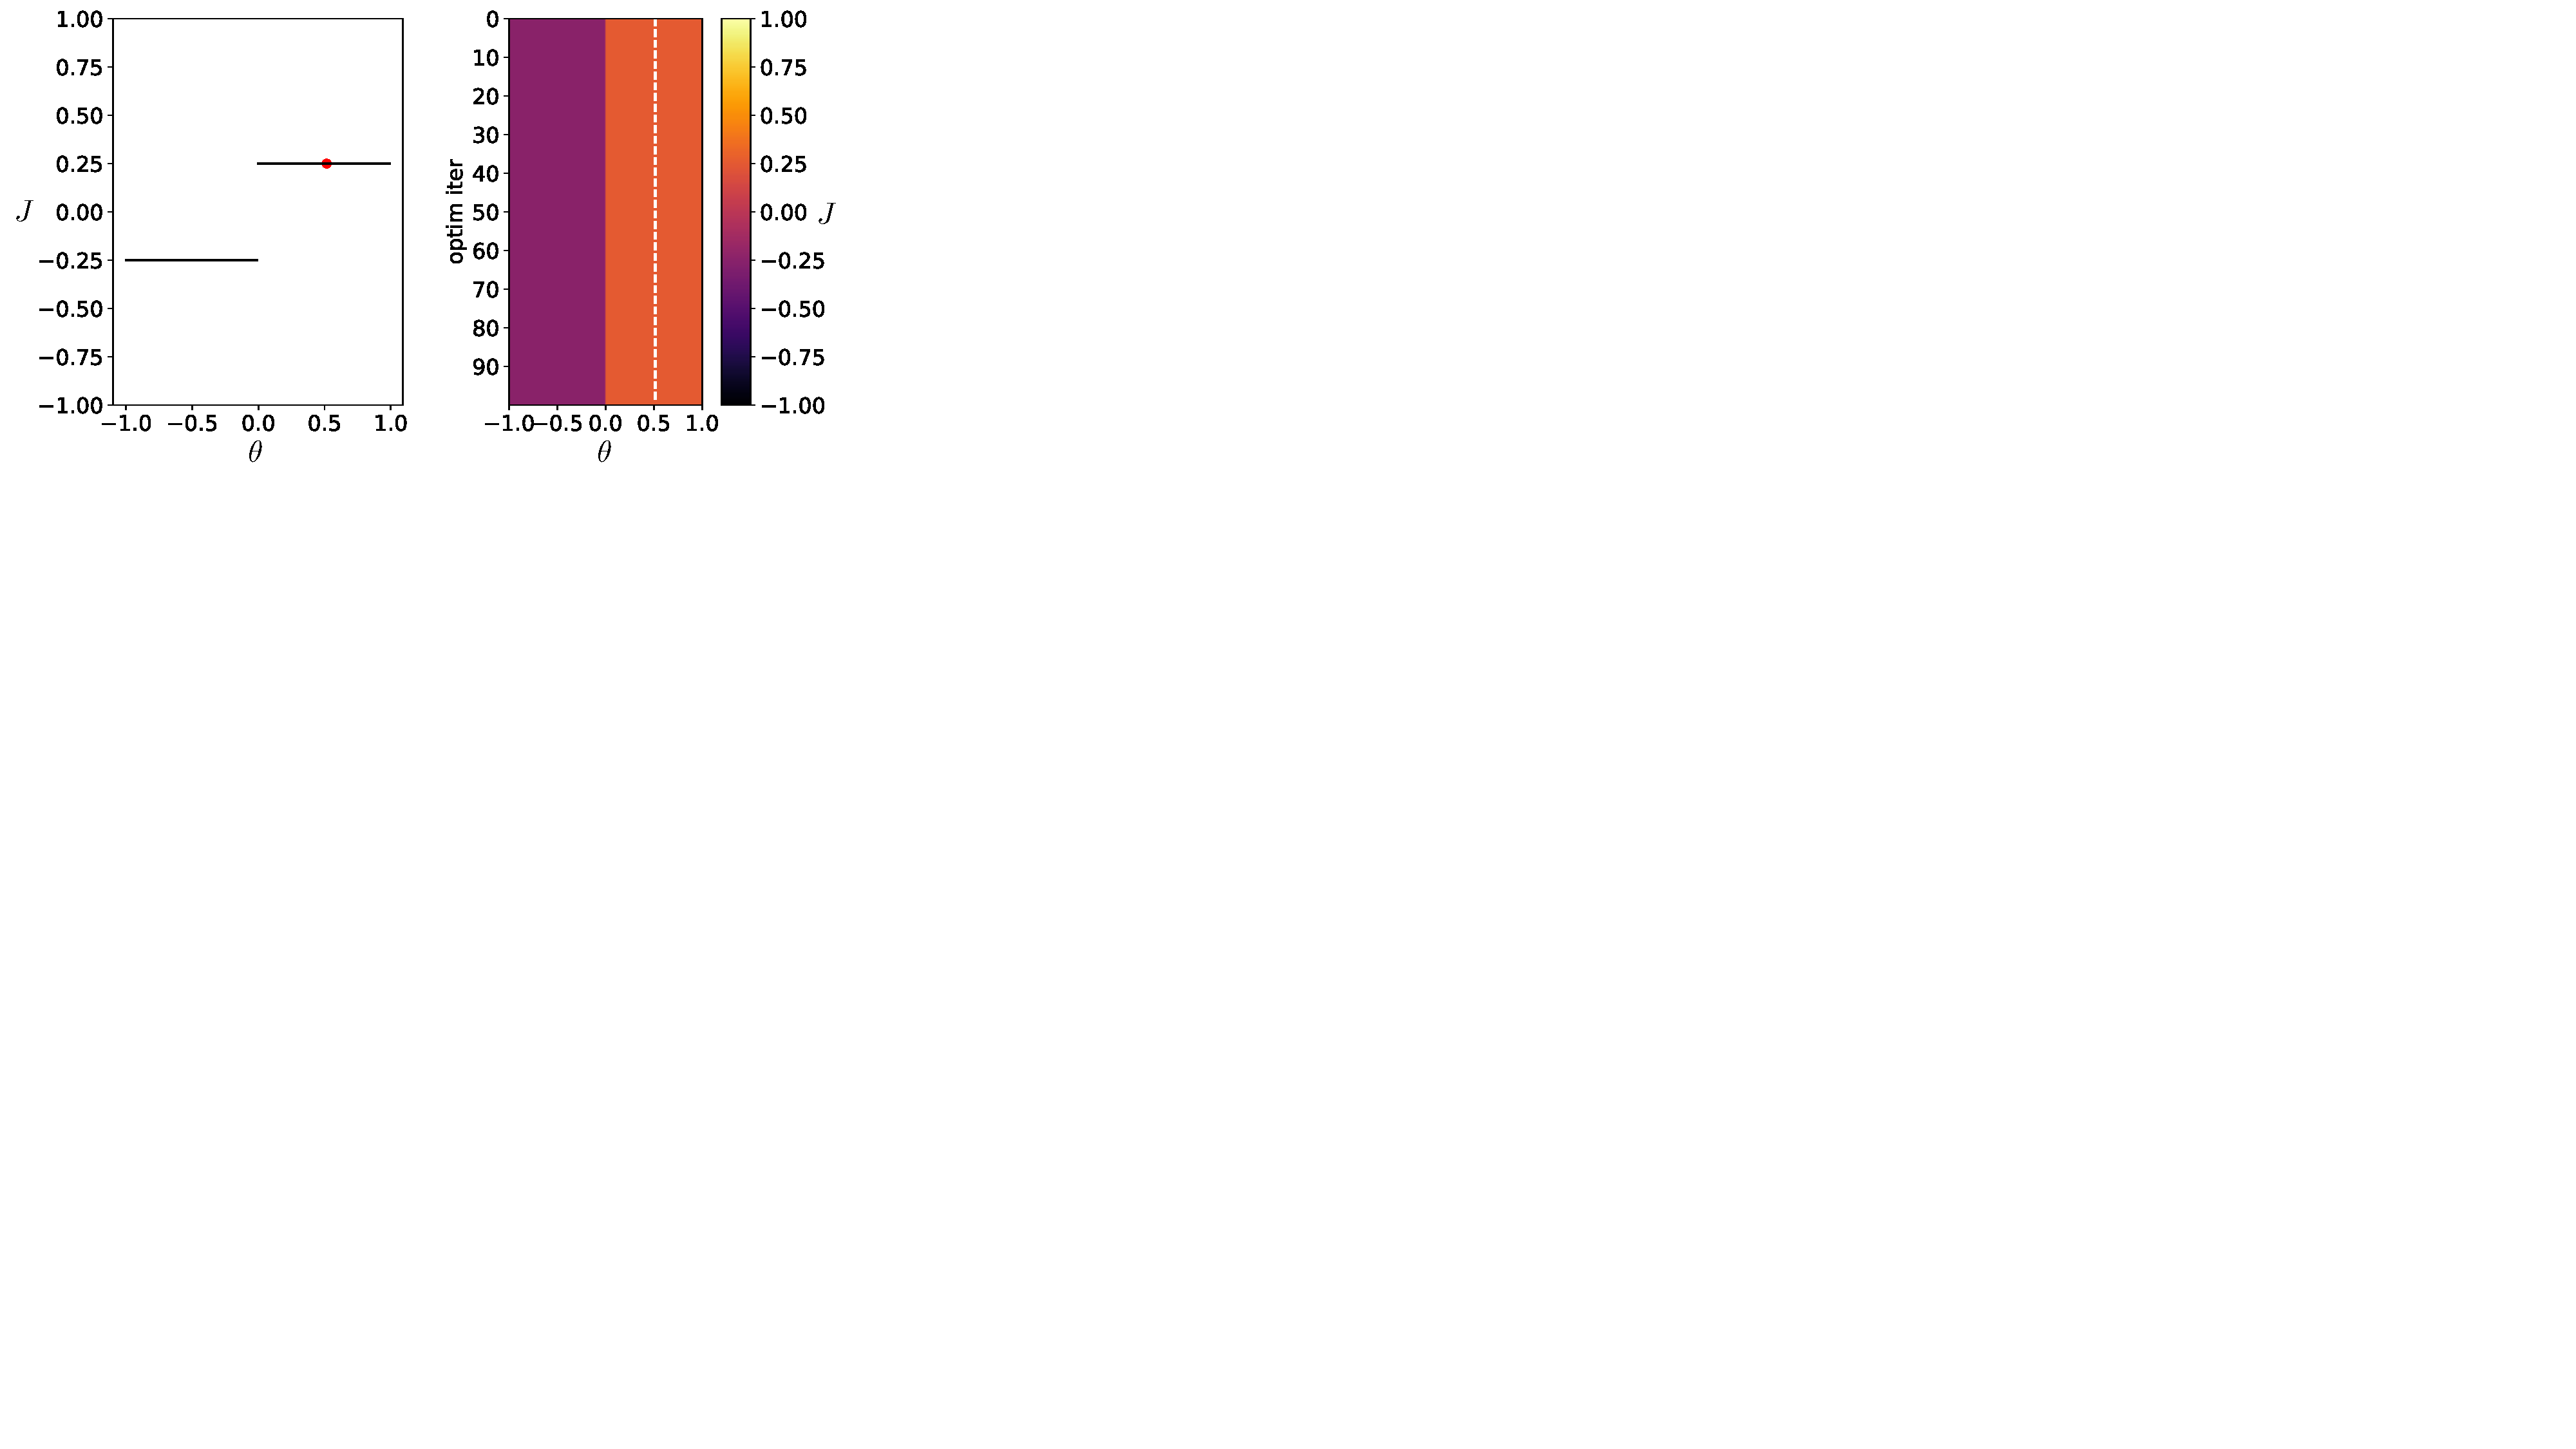
\includegraphics[width=0.5\linewidth]{./figures/gradient_descent/grad_descent_ex3.pdf} \\
        (e) exploding gradient & (f) multiple local minima \\
        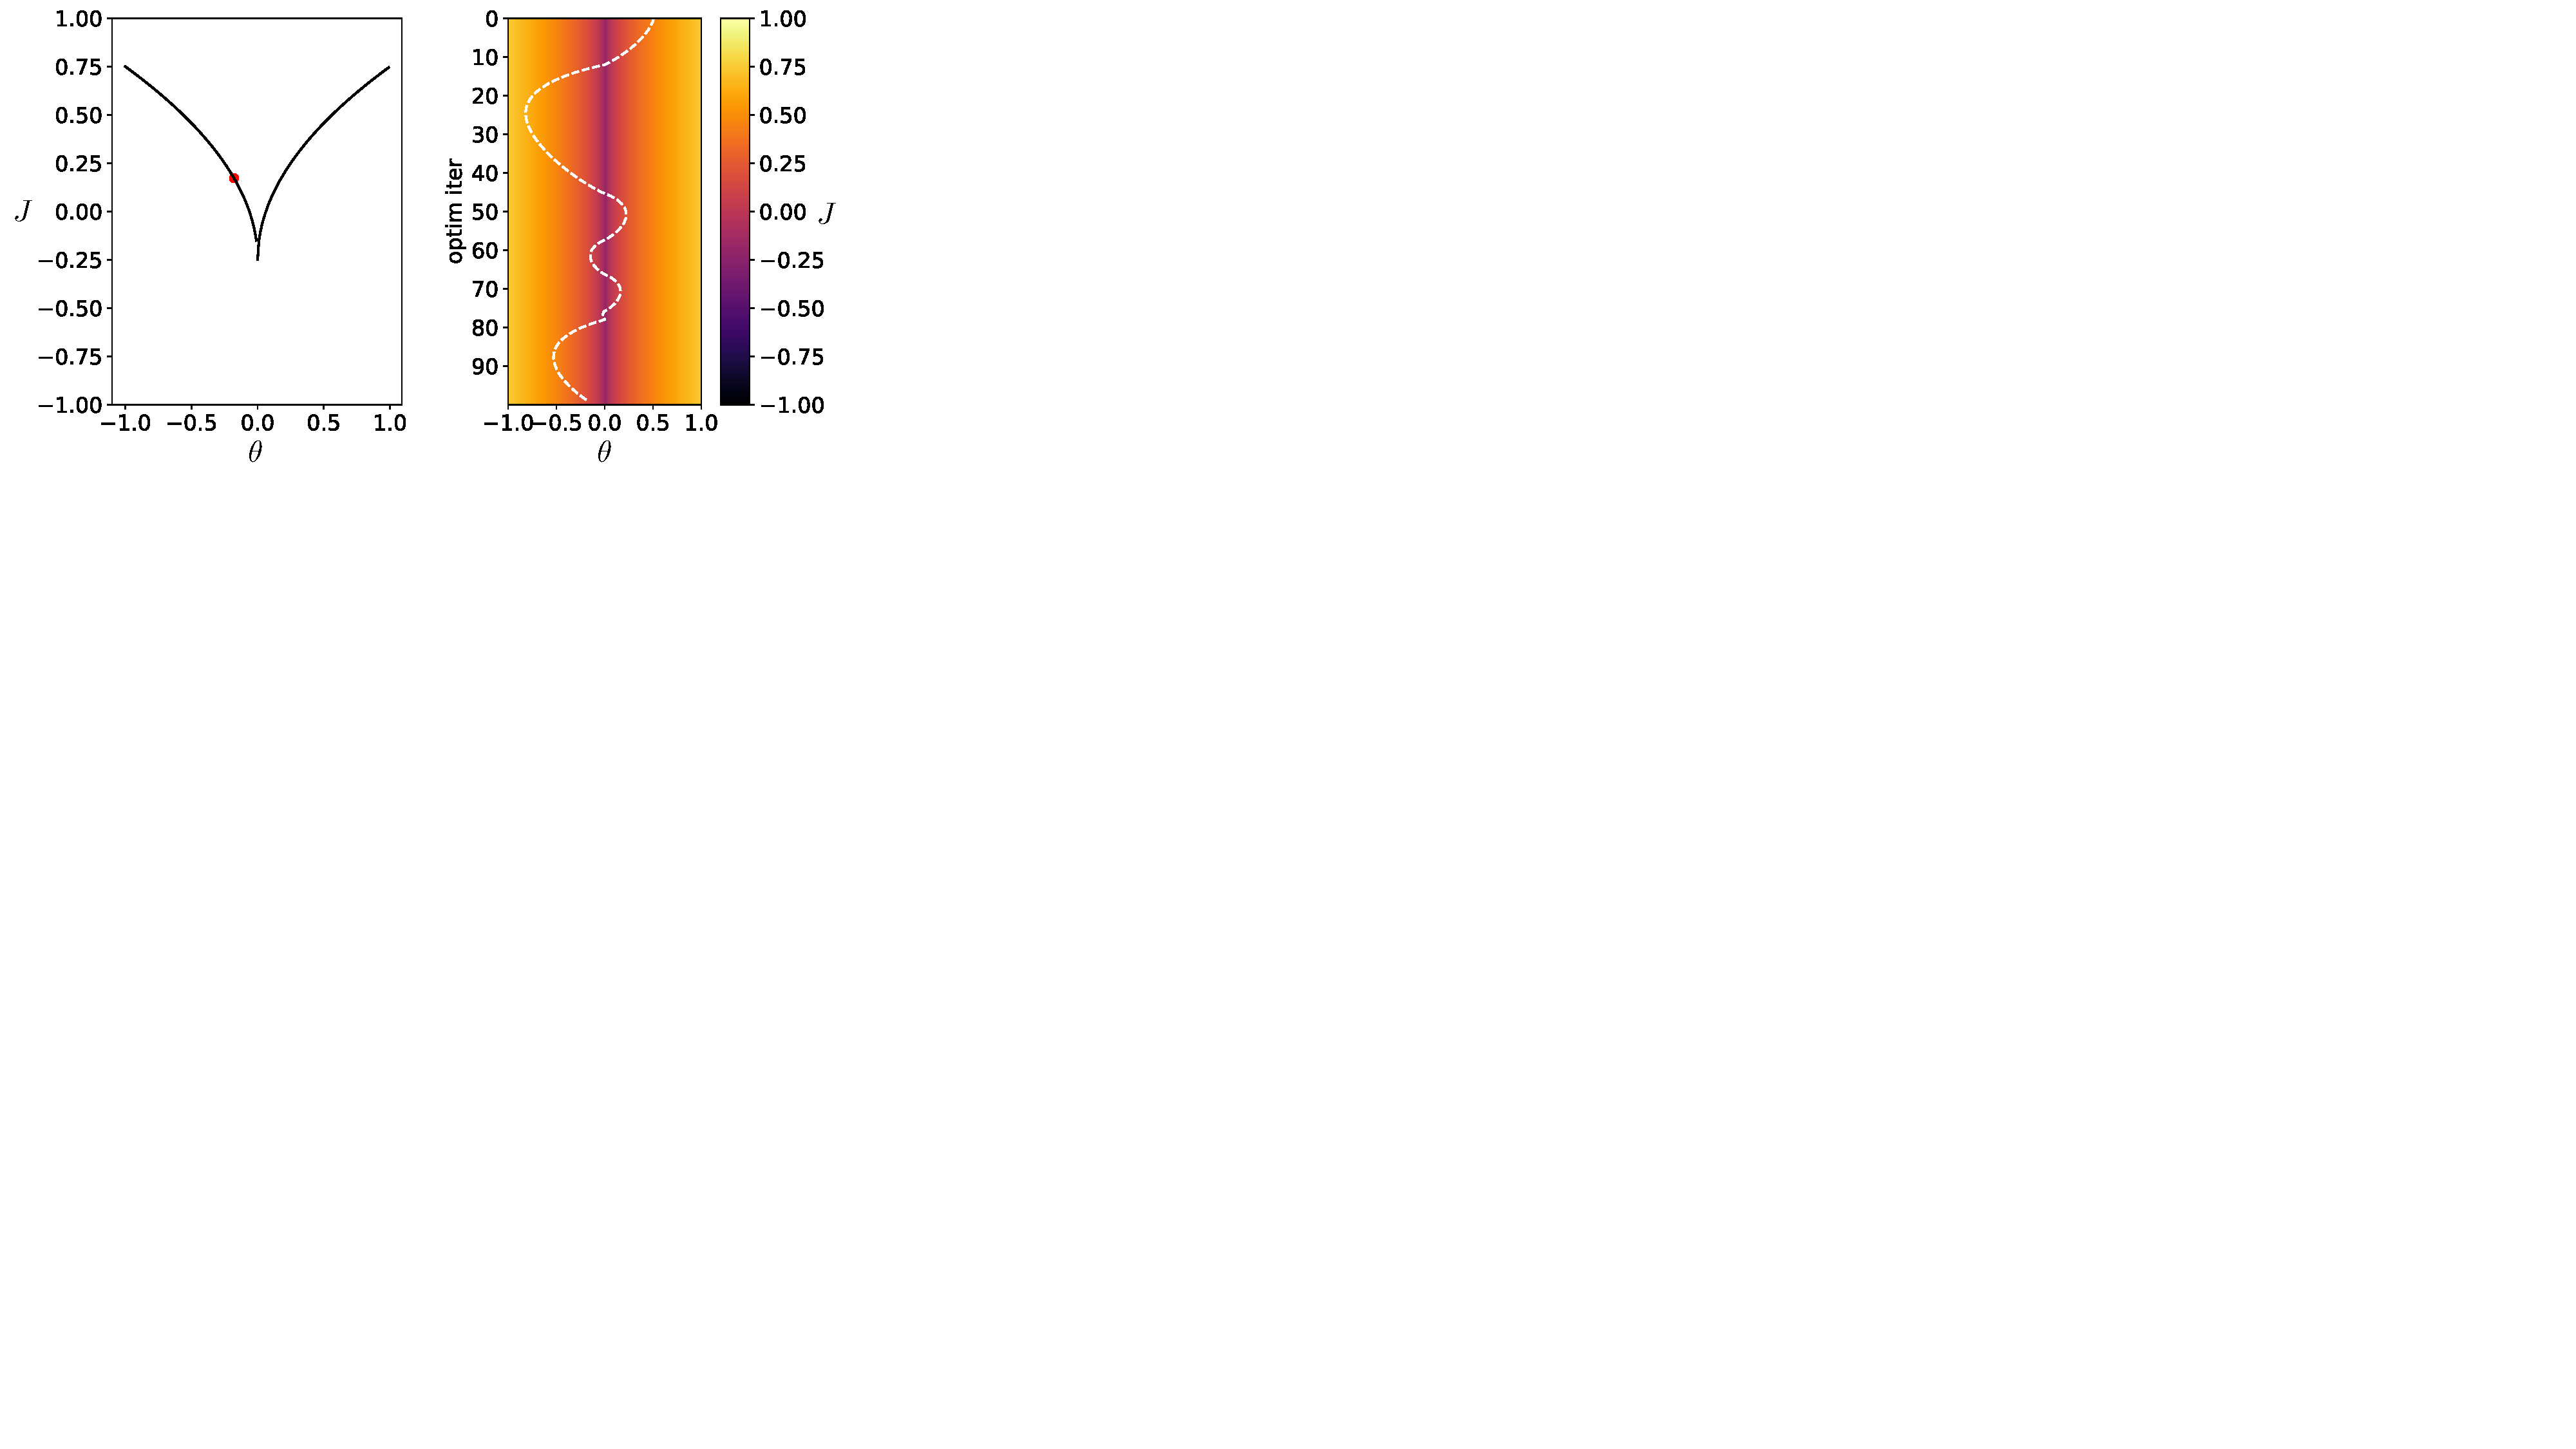
\includegraphics[width=0.5\linewidth]{./figures/gradient_descent/grad_descent_ex5.pdf} & 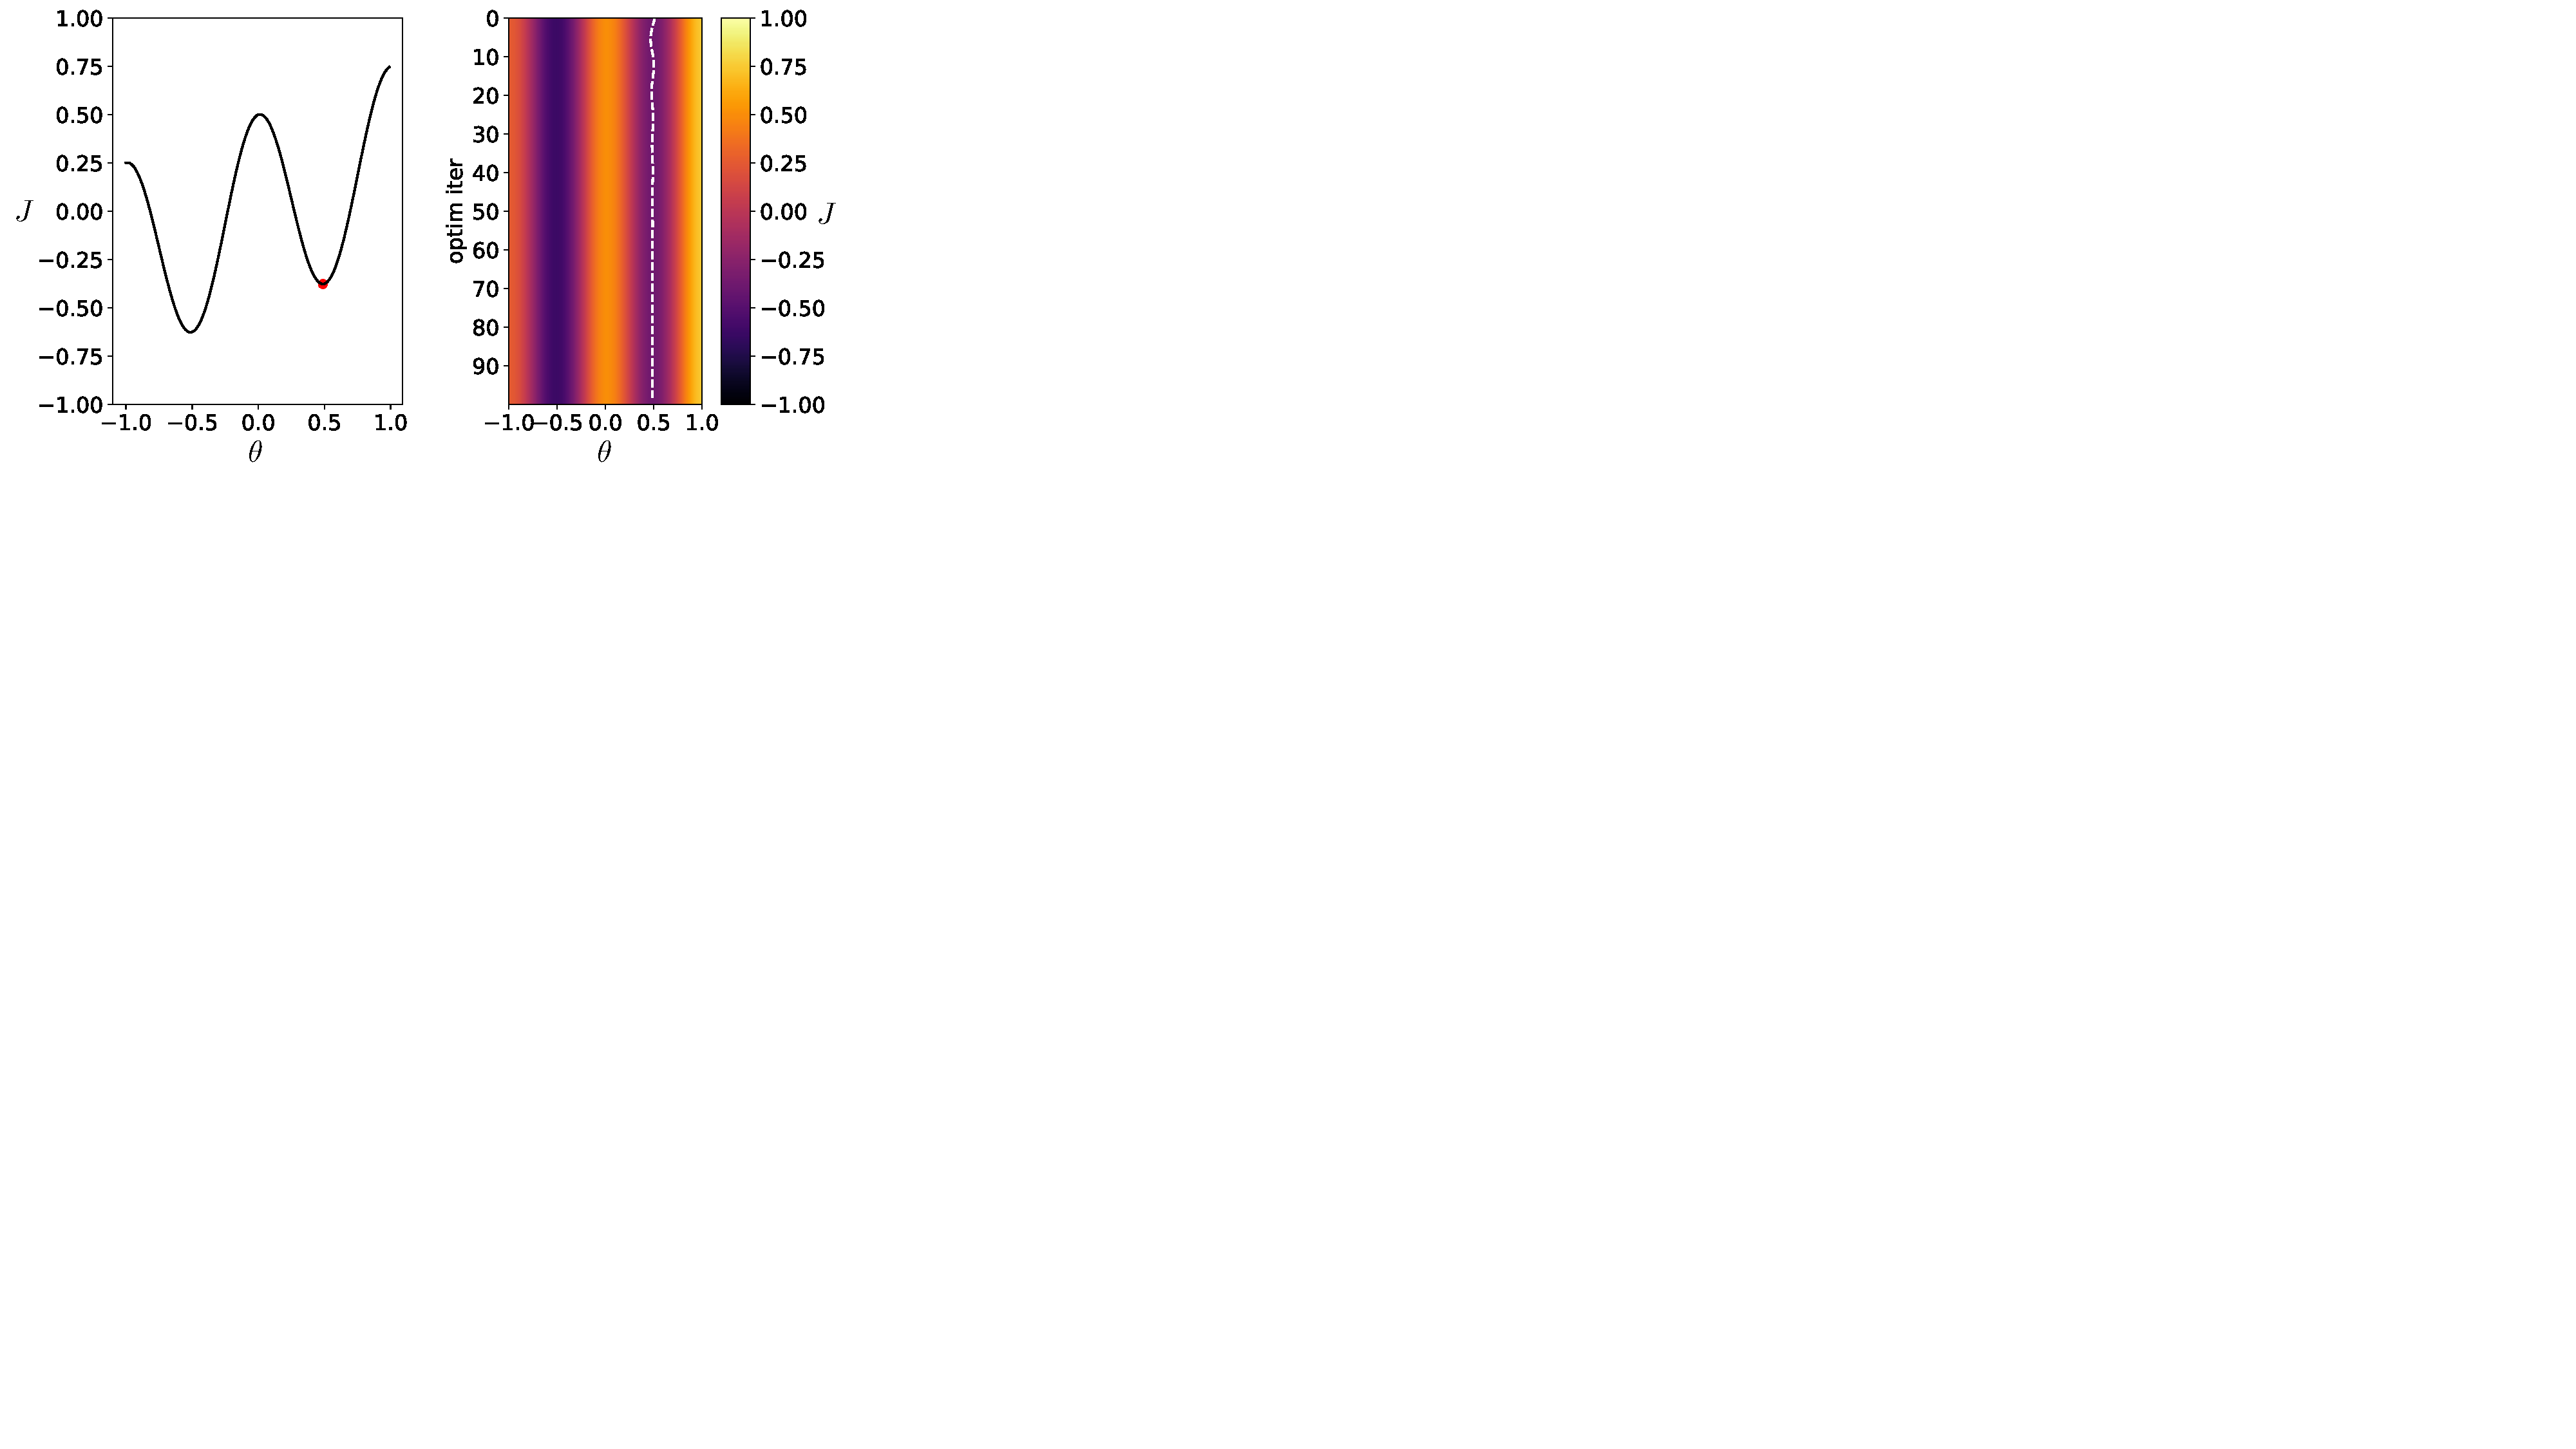
\includegraphics[width=0.5\linewidth]{./figures/gradient_descent/grad_descent_ex6.pdf}
    \end{tabular}
    }
    \caption{How gradient descent behaves on various functions. In each subplot, left is the function $J$, the red point is the solution found by $\GD$ (with $\eta=0.01$ and $\mu=0.9$), and right is the trajectory of $x$ values over iterations of $\GD$, plotted on top of $J$ at each iteration. (a) As $\eta$ goes to zero, $\GD$ converges for convex functions. (b) Discontinuities pose no essential problem, as long as the gradient is defined on either side. (c) A nearly flat function will exhibit very slow descent. (d) Piecewise constant functions are problematic because the gradient completely vanishes. (e) For the function $J=\texttt{sqrt}(\texttt{abs}(\theta))-0.25$, the gradient goes to infinity at the minimizer, causing instability. (f) When $J$ has multiple local minima, we may not find the global minimum.}
    \label{fig:gradient_descent:grad_descent_simple_examples}
\end{figure}


\subsection{Gradient-Like Optimization for Functions without Good Gradients}\label{sec:gradient_descent:zeroth_order}
What about minimizing functions like \fig{\ref{fig:gradient_descent:grad_descent_simple_examples}}(d), where the gradient is zero almost everywhere? This is a case where gradient descent truly struggles. However, it is often possible to transform such a problem into one that can be treated with gradient descent. Remember that the key property of a gradient, from the perspective of optimization, is that it is a locally loss-minimizing direction in parameter space. Most gradient-based optimizers don't really need true gradients; instead their update functions are compatible with a broader family of local loss-minimizing directions, $\mathbf{v}$. 

Besides the true gradient, what are some other good choices for $\mathbf{v}$? One common idea is to set $\mathbf{v}$ to be the gradient of a \index{Surrogate loss}\textbf{surrogate loss} function, which is a function, $J_{\texttt{surr}}$, with meaningful (non-zero) gradients, that approximates $J$. An example might be a smoothed version of $J$. Another way to get $\mathbf{v}$ is to compute it by sampling perturbations of $\theta$, and seeing which perturbation leads to lower loss. In this strategy, we evaluate $J(\theta+\epsilon)$ for a set of perturbations $\epsilon$, then move toward the $\epsilon$'s that decreased the loss. Approaches of this kind are sometimes called \index{Evolution strategies}\textbf{evolution strategies}~\cite{beyer2002evolution, salimans2017evolution}, and a basic version of this algorithm is given in \algref{\ref{alg:gradient_descent:ES}}.
%\vspace{-0.5cm}
\begin{algorithm}[h!]
\SetAlgoVlined
\DontPrintSemicolon
%\marginnote{{\bf Algorithm \ref{alg:gradient_descent:ES}}: Optimizing a cost function $J: \theta \rightarrow \mathbb{R}$ by evolution strategies, i.e., sampling different values for $\theta$ and taking a step toward the values that work best.}
\caption{{\bf Algorithm \ref{alg:gradient_descent:ES}}: Evolution strategies (\texttt{ES}). Optimizing a cost function $J: \theta \rightarrow \mathbb{R}$ by evolution strategies, i.e., sampling different values for $\theta$ and taking a step toward the values that work best.}
\fakealgorithmcaption{}
\label{alg:gradient_descent:ES}
{\bf Input:} objective function $J$, initial parameter vector $\theta^0$, learning rate $\eta$, sampling standard deviation $\sigma$, number of samples $M$, number of steps $K$\;%, data $\{\mathbf{x}^{(i)},\mathbf{y}^{(i)}\}_{i=1}^N$
{\bf Output:} trained parameter vector $\theta^* = \theta^K$\;
\For{\upshape $k= 0, \dots, K-1$}{
    \For{\upshape $i= 1, \dots, M$}{
        $\epsilon_i \sim \mathcal{N}(\mathbf{0},\mathbf{I})$\;
        $s_i = J(\theta + \sigma \epsilon_i)$\;
    }
    $\theta^{k+1} \leftarrow \theta^{k} - \eta \frac{1}{\sigma M}\sum^M_{i=1} s_i \epsilon_i$\;
}
\end{algorithm}
%\vspace{-0.5cm}

As shown in \fig{\ref{fig:gradient_descent:sampling_out1}}, this algorithm can successfully minimize the function in \fig{\ref{fig:gradient_descent:grad_descent_simple_examples}}(c).
\begin{figure}[h!]
    %\vspace{-0.75cm}
    \centerline{
    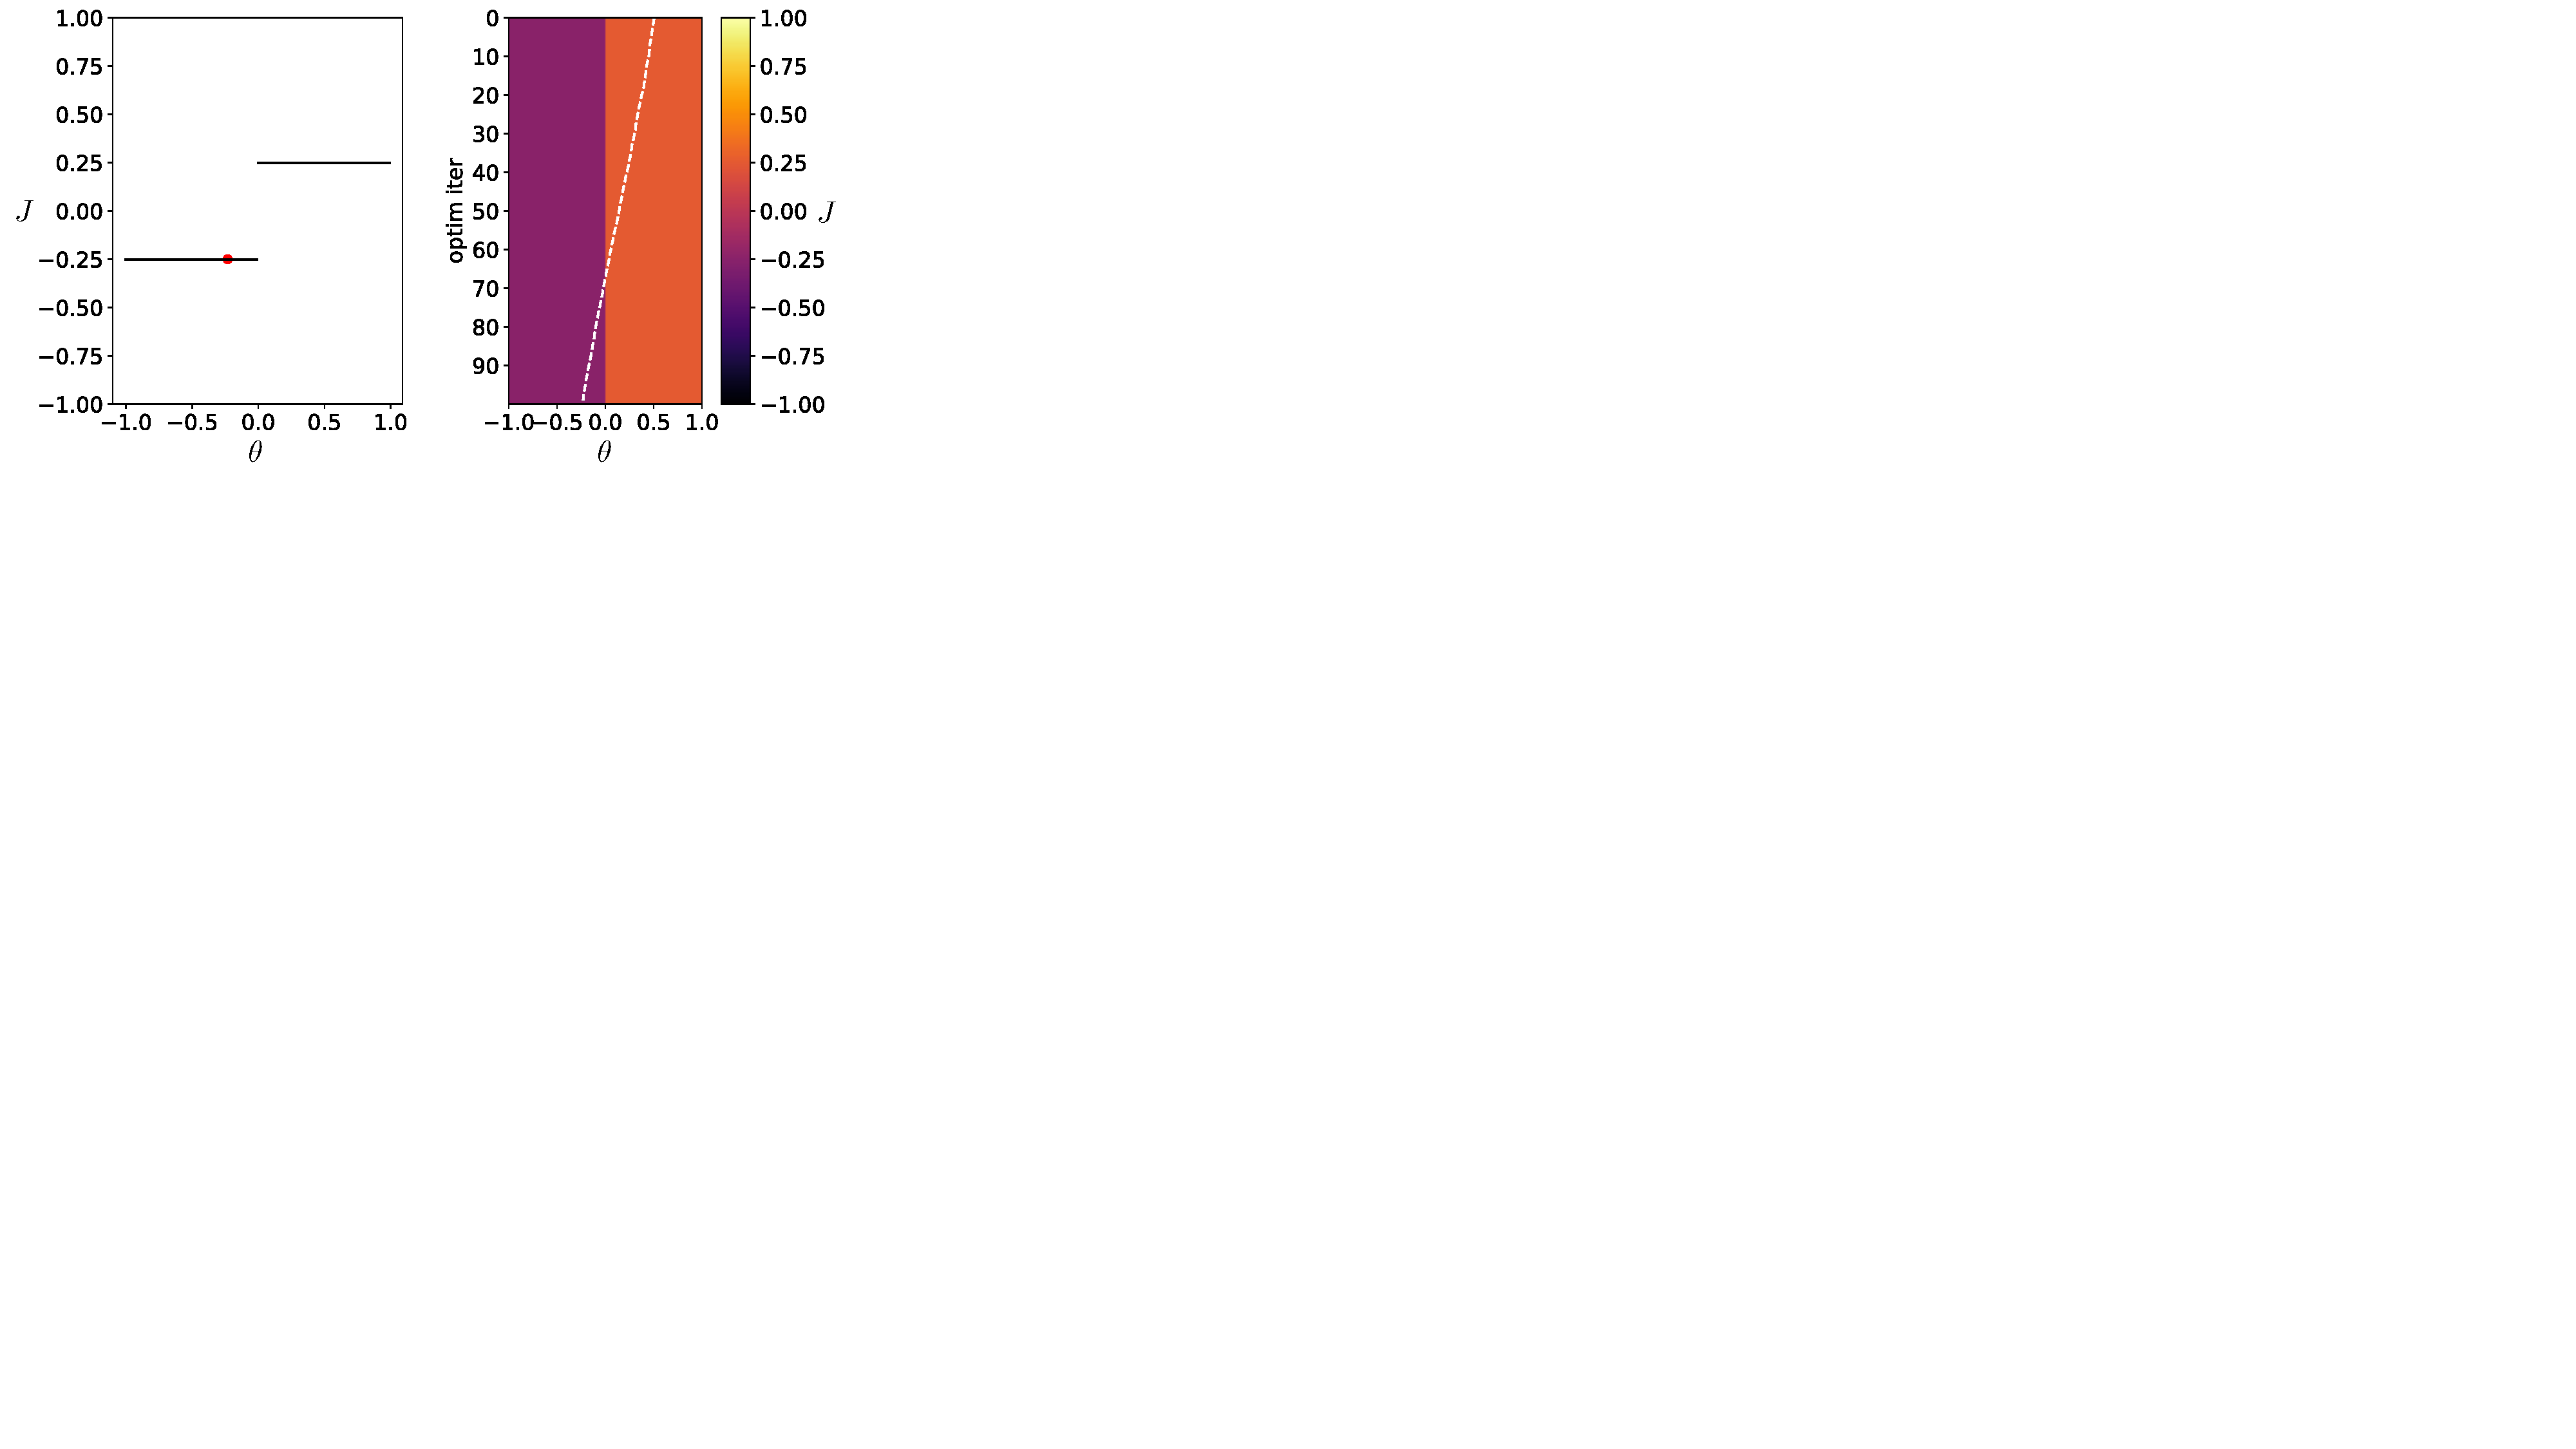
\includegraphics[width=0.5\linewidth]{./figures/gradient_descent/sampling_out1.pdf}
    }
    \caption{Using \ES~(\algref{\ref{alg:gradient_descent:ES}}) to minimize a nondifferentiable (zero-gradient) loss, using $\sigma=1$, $M=10$, and $\eta=0.02$.}
    \label{fig:gradient_descent:sampling_out1}
    %\vspace{-0.75cm}
\end{figure}

\subsection{Gradient Clipping}
What about \fig{\ref{fig:gradient_descent:grad_descent_simple_examples}}(e), where the gradient explodes near the optimum? Is there anything we can do to improve optimization of this function? To combat exploding gradients, a useful trick is \index{Gradient clipping}\textbf{gradient clipping}, which just means clamping the magnitude of the gradient to some maximum value. \Algref{\ref{alg:gradient_descent:grad_clipping}} describes this approach.

\begin{algorithm}[h]
\SetAlgoVlined
\DontPrintSemicolon
%\marginnote{{\bf Algorithm \ref{alg:gradient_descent:grad_clipping}}: Gradient descent with gradient clipping.}
\caption{{\bf Algorithm \ref{alg:gradient_descent:grad_clipping}}: Gradient descent with gradient clipping.}
\fakealgorithmcaption{}
\label{alg:gradient_descent:grad_clipping}
{\bf Input:} objective function $J$, initial parameter vector $\theta^0$, learning rate $\eta$, number of steps $K$, max gradient magnitude $m$\;%, data $\{\mathbf{x}^{(i)},\mathbf{y}^{(i)}\}_{i=1}^N$
{\bf Output:} trained parameter vector $\theta^* = \theta^K$\;
\For{\upshape $k= 0, \dots, K-1$}{
    %$J = \sum_{i=1}^N \mathcal{L}(f_{\theta^{k-1}}(\mathbf{x}^{(i)}),\mathbf{y}^{(i)})$\;
    $\mathbf{v} = \nabla_{\theta} J(\theta^k)$\;
    %$\theta^{k+1} \leftarrow \theta^{k} - \eta %[\max(\min(v_1,m),-m),\ldots,\max(\min(v_M,m),-m)]^\transpose$\; %\quad\quad \triangleleft \text{per-dimension clipping}$\;
    %$\theta^{k} \leftarrow \theta^{k-1} - \eta \min(\norm{\mathbf{v}},m)\frac{\mathbf{v}}{\norm{\mathbf{v}}}$\;
     $\theta^{k+1} \leftarrow \theta^{k} - \eta [\texttt{clip}(v_1, -m, m), \ldots, \texttt{clip}(v_M, -m, m)]^\transpose$
}
\end{algorithm}
\marginnote{\texttt{clip} is the ``clipping'' function: $\texttt{clip}(v, -m, m) = \max(\min(v,m),-m)$}[-1.6cm]

This algorithm indeed successfully minimizes our example of the exploding gradient, as can be seen in \fig{\ref{fig:gradient_descent:clipped_out1}}.
\begin{figure}[h]
    \centerline{
    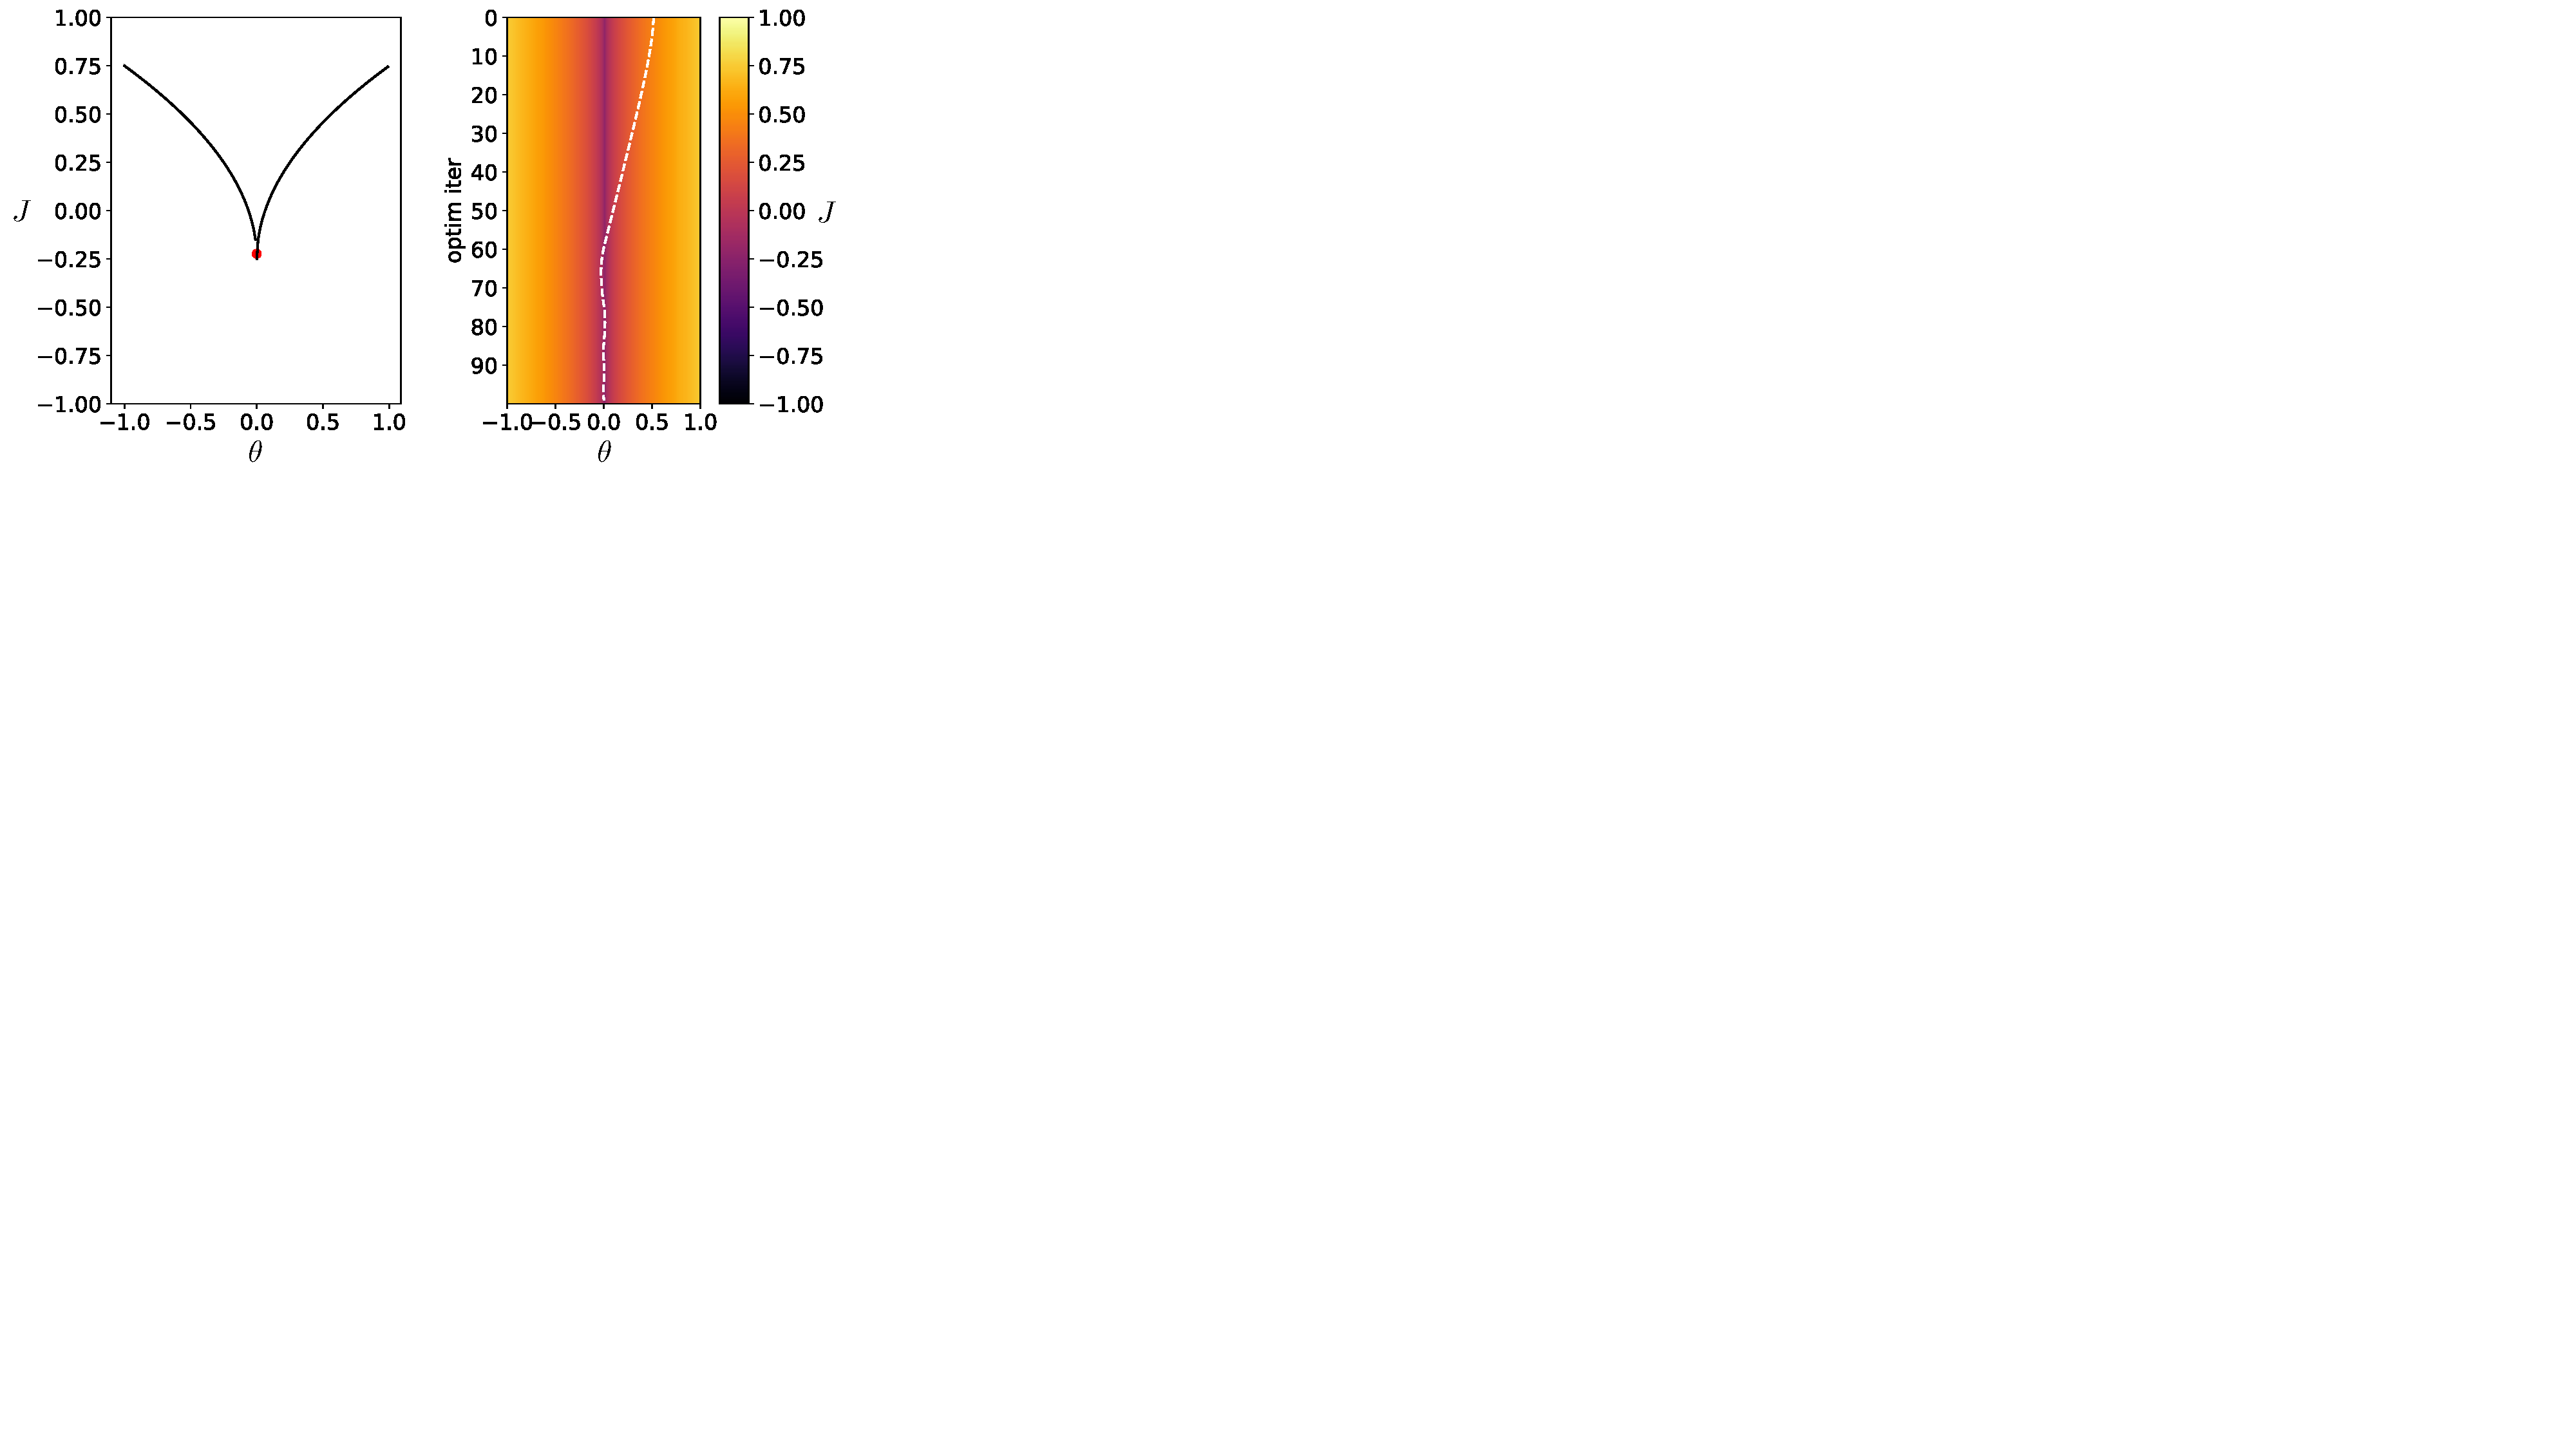
\includegraphics[width=0.5\linewidth]{./figures/gradient_descent/clipped_out1.pdf}
    }
    \caption{Using \GD~with clipping to minimize a loss with exploding gradients, using $m=0.1$.}
    \label{fig:gradient_descent:clipped_out1}
\end{figure}

%This is a case where gradient descent truly struggles. However, with a small modification, gradient descent again becomes applicable. The modification is to descend the gradient of a smooth approximation to $J$, which we will call $J_{\texttt{smooth}}$, rather than to $J$ itself. Given some data, we can either \textit{globally} fit $J_{\texttt{smooth}}$ to $J$, then plug $J_{\texttt{smooth}}$ into Algorithm \ref{alg:gradient_descent:basic_gradient_descent}, or we can proceed in an ``online" fashion, where on each iteration of gradient descent, we \textit{locally} compute: just for this operating point what is the smooth gradient? The latter can be more efficient since we only have to do the approximation for the operating points we visit, which may be a very small subspace of the total parameter space. For this approach, in practice, on each iteration of gradient, we may sample \textbf{finite differences} to find the locally linear approximation to the loss surface:

%The property that we need is that at each operating point, a loss-minimizing direction, $\mathbf{v}$, can given as the input to the update function. This gradient 

% \begin{figure}[h]
%     \centering
%     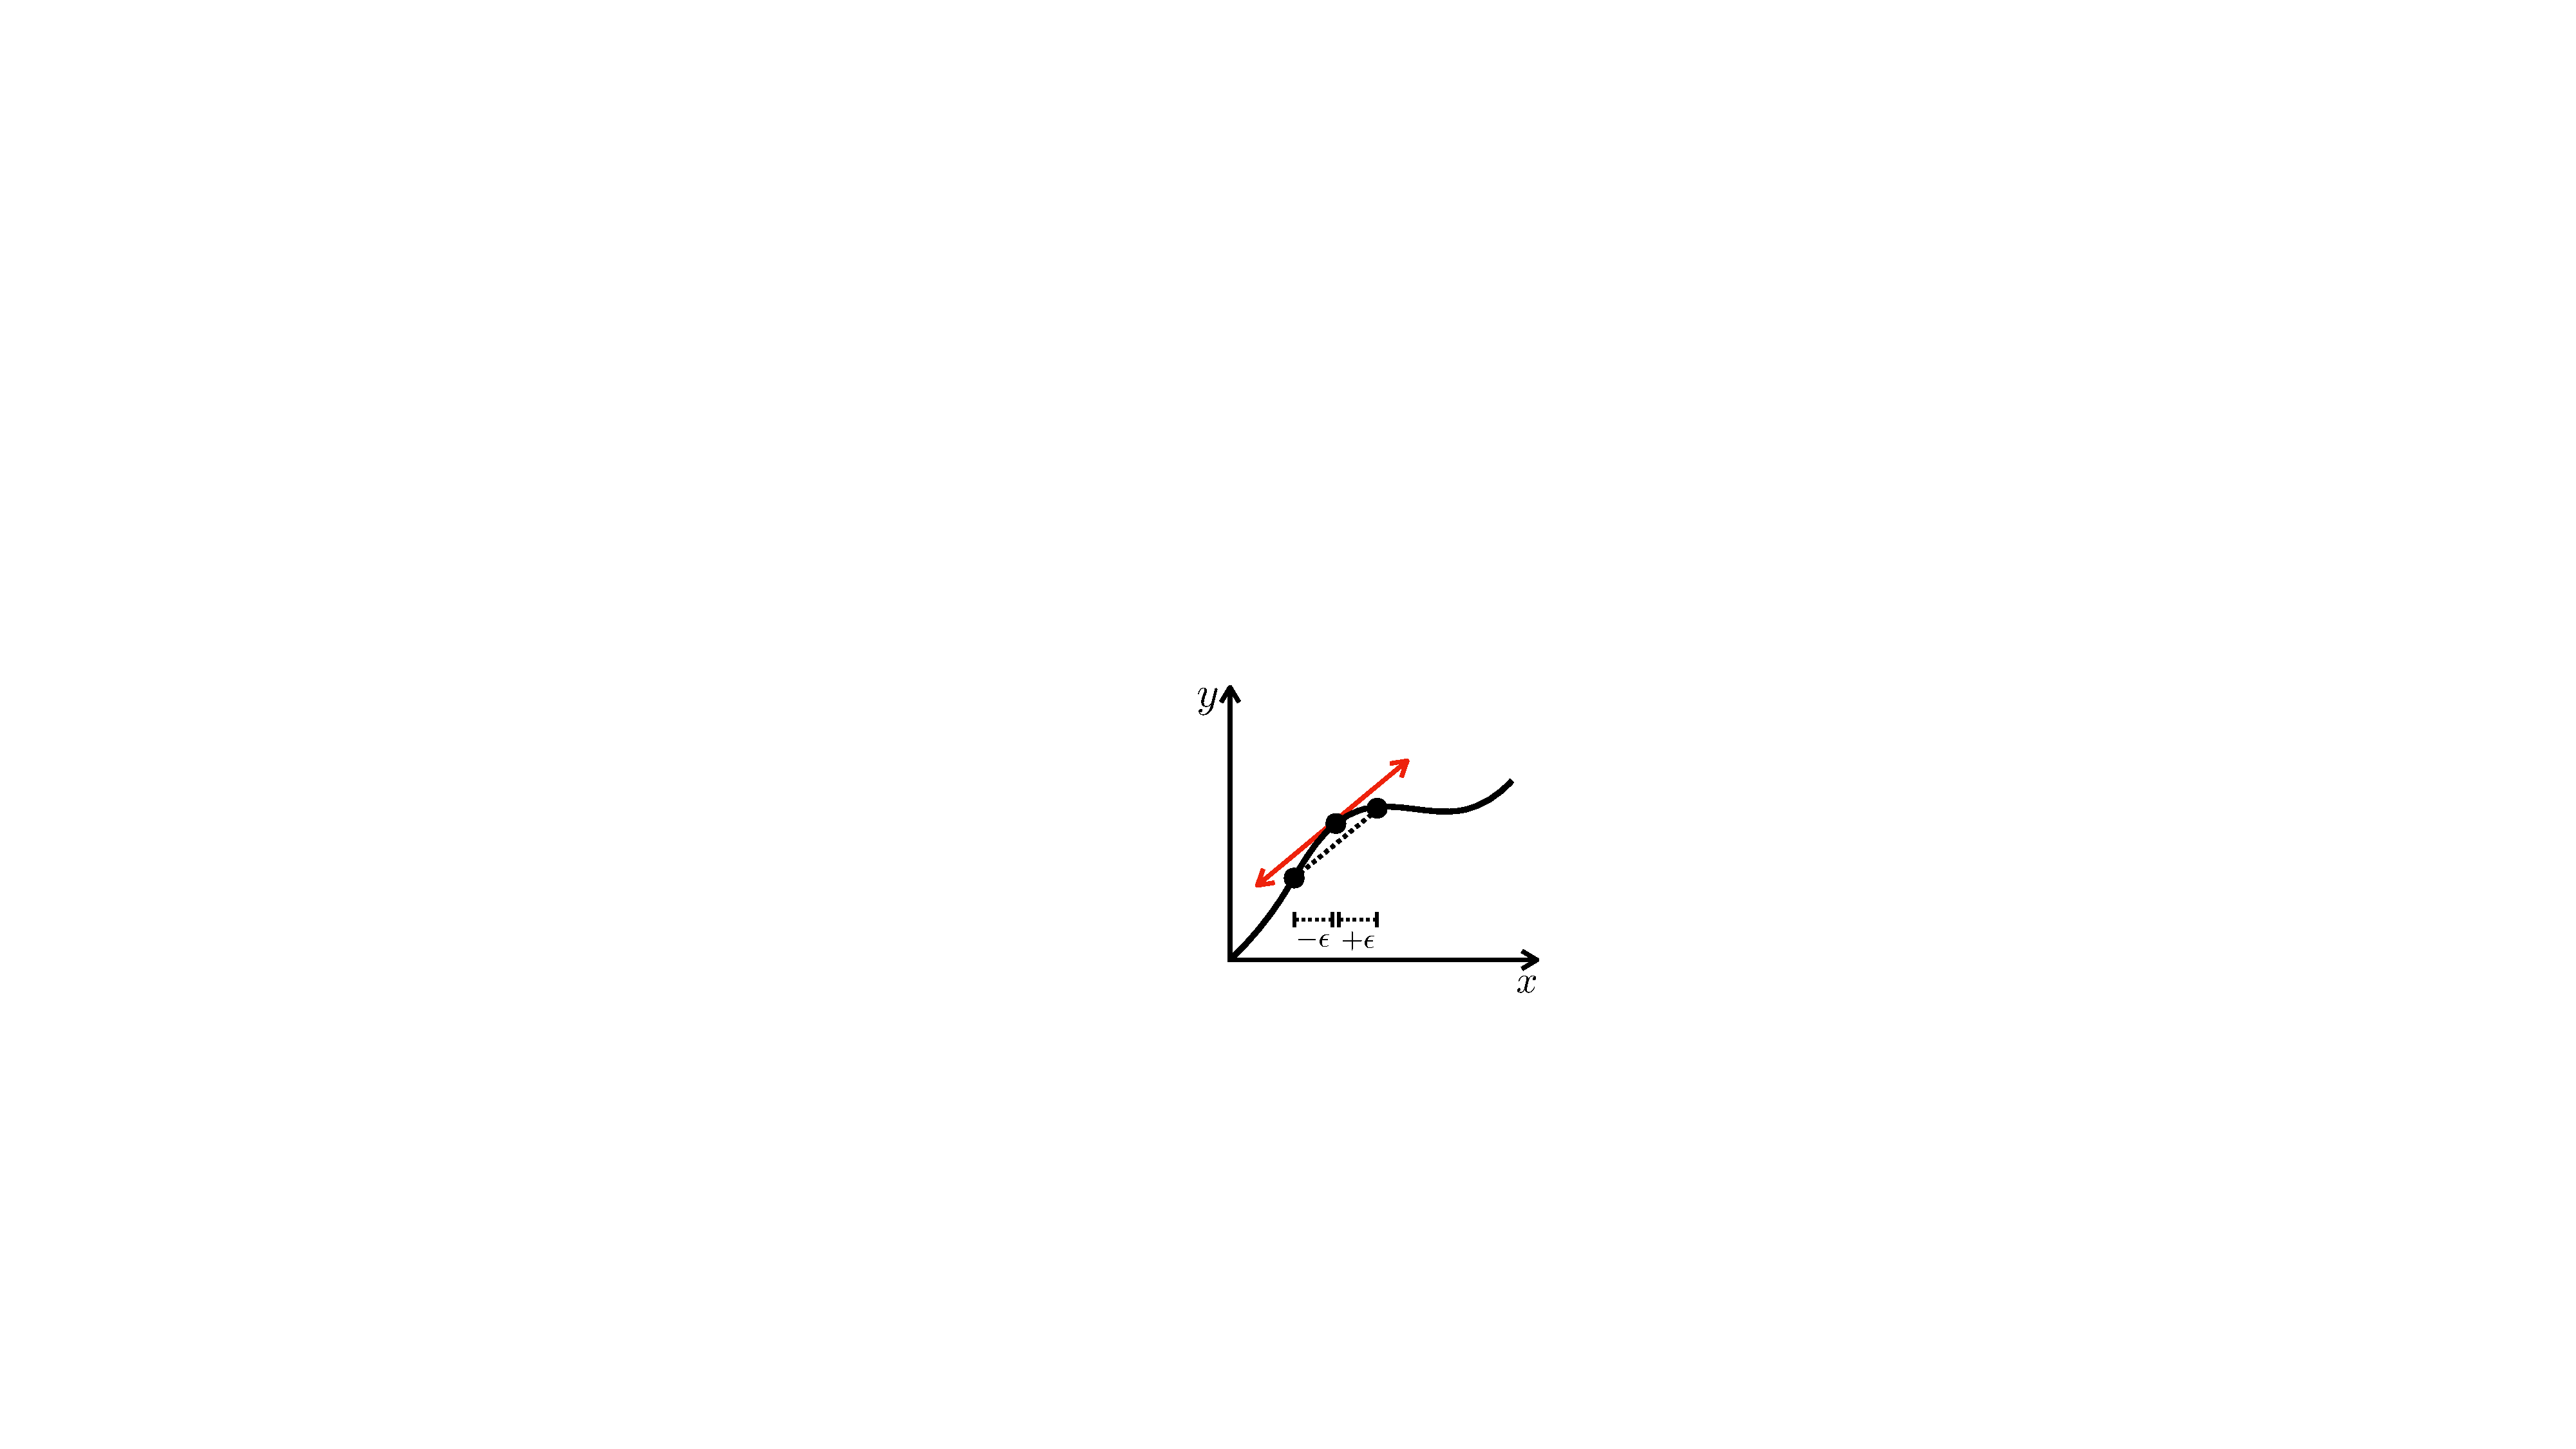
\includegraphics[width=0.35\linewidth]{./figures/gradient_descent/finite_diffs.pdf}
%     \label{fig:gradient_descent:finite_diffs}
% \end{figure}


%\section{Learning rate schedules}


\section{Stochastic Gradient Descent}\label{sec:gradient_descent:SGD}

One problem with the gradient-based methods we have seen so far is that the gradient may in fact be very expensive to compute, and this is often the case for learning problems. This is because learning problems typically have the form that $J$ is the average of losses incurred on each training datapoint. Computing $\nabla_{\theta}J(\theta)$ requires computing the gradient for each element in the average, that is, the gradient of the function being learned evaluated at the location of each datapoint in the training set. If we train on a big dataset, say 1 million training points, then to perform just \textit{one} step of gradient descent requires computing 1 million gradients! %. If we train on big data, which often we want to do, then even just evaluating $J$, or its gradient, will be expensive.
To make this clear, we will write out $J$ as an explicit function of the training data $\{\mathbf{x}^{(i)}, \mathbf{y}^{(i)}\}_{i=1}^N$. For typical learning problems, $\nabla_{\theta} J(\theta, \{\mathbf{x}^{(i)}, \mathbf{y}^{(i)}\}_{i=1}^N)$ decomposes as follows:
\begin{align}
    \nabla_{\theta} J(\theta, \{\mathbf{x}^{(i)}, \mathbf{y}^{(i)}\}_{i=1}^N) &= %\frac{1}{N}\sum_{i=1}^N \nabla_{\theta} \mathcal{J}(\theta, \mathbf{x}^{(i)}, \mathbf{y}^{(i)})\\
    %&= 
    \nabla_{\theta} \frac{1}{N}\sum_{i=1}^N \mathcal{L}(f_{\theta}(\mathbf{x}^{(i)}), \mathbf{y}^{(i)})\\
    &= \frac{1}{N}\sum_{i=1}^N \nabla_{\theta} \mathcal{L}(f_{\theta}(\mathbf{x}^{(i)}), \mathbf{y}^{(i)})
\end{align}

For large $N$, computing this sum is very expensive. Suppose instead we randomly subsample (without replacement) a \textit{batch} of terms from this sum, $\{\mathbf{x}^{(b)}, \mathbf{y}^{(b)}\}_{b=1}^B$, where $B$ is the \index{Batch size}\textbf{batch size}. We then compute an \textit{estimate} of the total gradient as the average gradient over this batch as follows:
\begin{align}
    \tilde{\mathbf{g}} = \frac{1}{N}\sum_{b=1}^B \nabla_{\theta} \mathcal{L}(f_{\theta}(\mathbf{x}^{(b)}), \mathbf{y}^{(b)})
\end{align}
If we sample a large batch, where $B$ is almost as large as $N$, then the average over the $B$ terms should be roughly the same as the average over all $N$ terms. If we sample a smaller batch, then our estimate of the gradient will be less accurate but faster to compute. Therefore we have a tradeoff between accuracy and speed, and we can navigate this tradeoff with the hyperparameter $B$. The variant of gradient descent that uses this idea is called \index{Stochastic gradient descent}\textbf{stochastic gradient descent} (SGD), because each iteration of descent uses a different randomly (stochastically) sampled batch of training data to estimate the gradient. The full description of \SGD~is given in \algref{\ref{alg:gradient_descent:SGD}}.
\begin{algorithm}[h]
\SetAlgoVlined
\DontPrintSemicolon
%\marginnote{{\bf Algorithm \ref{alg:gradient_descent:SGD}}: Stochastic gradient descent estimates the gradient from a stochastic subset (batch) of the full training data, and makes an update on that basis.}
\caption{{\bf Algorithm \ref{alg:gradient_descent:SGD}}: Stochastic gradient descent (\SGD). Stochastic gradient descent estimates the gradient from a stochastic subset (batch) of the full training data, and makes an update on that basis.}
\fakealgorithmcaption{}
\label{alg:gradient_descent:SGD}
{\bf Input:} initial parameter vector $\theta^{0}$, data $\{\mathbf{x}^{(i)},\mathbf{y}^{(i)}\}_{i=1}^N$, learning rate $\eta$, batch size $B$, number of steps $K$\;
{\bf Output:} trained parameter vector $\theta^* = \theta^K$\;
\For{\upshape $k= 0, \dots, K-1$}{
    $\{\mathbf{x}^{(b)},\mathbf{y}^{(b)}\}_{b=1}^B \sim \{\mathbf{x}^{(i)},\mathbf{y}^{(i)}\}_{i=1}^N \quad\quad \triangleleft \text{ sample batch of training data}$\;
    $\tilde{\mathbf{g}} = \frac{1}{N}\sum_{b=1}^B \nabla_{\theta} \mathcal{L}(f_{\theta}(\mathbf{x}^{(b)}), \mathbf{y}^{(b)})$\;
    $\theta^{k} \leftarrow \theta^{k-1} - \eta \tilde{\mathbf{g}}$\;
}
\end{algorithm}

\SGD~has a number of useful properties beyond just being faster to compute than \GD. Because each step of descent is somewhat random, \SGD~can jump over small bumps in the loss landscape, as long those bumps disappear for some randomly sampled batches. Another important property is that \SGD~can implicitly regularize the learning problem. For example, for linear problems (i.e., $f_\theta$ is linear), then if there are multiple parameter settings that minimize the loss, \SGD~will often converge to the solution with minimum parameter norm~\cite{zhang2021understanding}.

%\section{How to initialize?}

% \section{Parameterization matters}
% \reviewcomment{Unfinished section.}
% \subsection{The power of overparameterization}
% Show a problem where the overparameterized loss landscape has smooth paths of descent (around obstacles) but the less-parameterized loss landscape does not.

\section{Concluding Remarks}
The study of optimization can fill dozens of textbooks and thousands of academic papers. But fortunately for us, modern machine learning has converged on just a few very simple optimization methods that are used in practice. We will soon encounter deep learning, which is the main kind of machine learning used for computer vision. In deep learning, gradient-based optimization is the workhorse. Believe it or not, the handful of algorithms described above are enough to train most state-of-the-art deep learning models. Every year there are new elaborations on these ideas, and second-order methods are ever on the horizon, yet the basic concepts remain quite simple: compute a local estimate of the shape of the loss landscape, then, based on this shape, take a small step toward a lower loss.
%Sometimes this is even treated as definitional to deep learning: deep learning is learning with gradient-based optimization. % PHILLIP
% %\setcounter{chapter}{7}

\chapter{The Problem of Generalization}\label{chapter:problem_of_generalization}

\section{Introduction}

So far, we have described learning as an optimization problem: maximize an objective over the \emph{training set}. But this is not our actual goal. Our goal is to maximize the objective over the \emph{test set}. This is the key difference between learning and optimization. We do not have access to the test set, so we use optimization on the training set as a proxy for optimization on the test set. 

Learning theory studies the settings under which optimization on the training set yields good results on the test set. In general it may not, since the test set may have different properties from the training set. When we fit to properties in the training data that do not exist in the test data, we call this {\bf overfitting}. When this happens, training performance will be high, but test performance can be very low, since what we learned about the training data does not {\bf generalize} to the test data.

\section{Underfitting and Overfitting}

A learner may perform poorly for one of two reasons: either it failed to optimize the objective on the training data, or it succeeded on the training data but in a way that does not generalize to the test setting. The former is called \index{Underfitting}{\bf underfitting} and the latter is called \index{Overfitting}{\bf overfitting}.

We will walk through a concrete example of a learner, polynomial regression, that exemplifies these two effects. We introduce this learner briefly in the next subsection before exploring what it tells us about underfitting, overfitting, and generalization.

\subsection{Background: The Polynomial Regression Learning Problem}
Polynomial regression is just like linear regression (\chap{\ref{chapter:intro_to_learning}}) except that the hypothesis space is polynomial functions rather than linear functions, that is,
\begin{align}
y = f_{\theta}(x) = \sum_{k=0}^K \theta_k x^k
\end{align}
where $K$, the degree of the polynomial, is a hyperparameter of the hypothesis space.

Let us consider the setting where we use the least-squares ($L_2$) loss function. It turns out polynomial regression is highly related to linear regression; in fact, we can transform a polynomial regression problem into a linear regression problem! We can see this by rewriting the polynomial as:
\begin{align}
    \sum_{k=0}^K \theta_k x^k = \theta^\transpose\phi(x)\\
    \quad\quad\quad\quad \phi(x) = \begin{bmatrix}
                            1 \\ x \\ x^2 \\ \vdots \\ x^K
                        \end{bmatrix}
\end{align}
Now the form of $f_{\theta}$ is $f_{\theta}(x) = \theta^\transpose\phi(x)$, \textit{which is a linear function in the parameters $\theta$}. Therefore, if we \textit{featurize} $x$, representing each datapoint $x$ with a feature vector $\phi(x)$, then we have arrived at a linear regression problem in this feature space. So, the learning problem, and closed form optimizer, for $L_2$ polynomial regression looks almost identical to that of $L_2$ linear regression:

\begin{center}
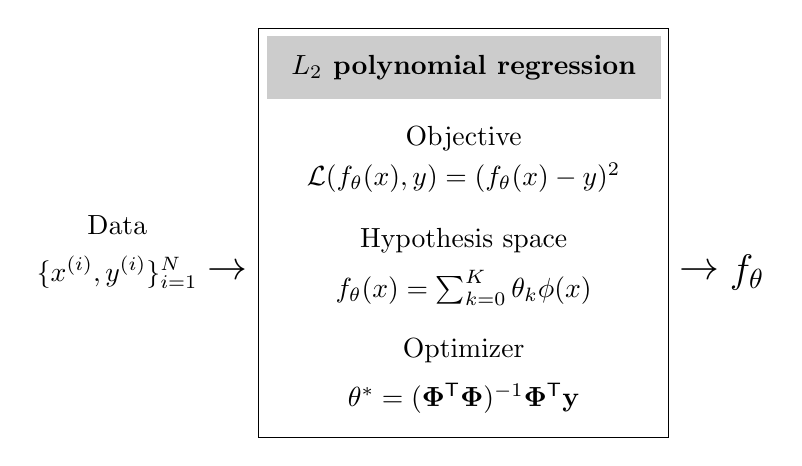
\begin{tikzpicture}
    \draw (0,0) rectangle (5.2,5.2); % outer box
    \fill[black!20] (0.1,4.3) rectangle (5.1,5.1); % gray box
    \node[] at (2.6,4.7) {{\bf $L_2$ polynomial regression}};
    \node[] at (2.6,3.8) {Objective}; \node[] at (2.6,3.3) {$\mathcal{L}(f_{\theta}(x),y) = (f_{\theta}(x)-y)^2$};
    \node[] at (2.6,2.5) {Hypothesis space}; \node[] at (2.6,1.9) {$f_{\theta}(x) = \sum_{k=0}^K \theta_k \phi(x)$};
    \node[] at (2.6,1.1) {Optimizer}; \node[] at (2.6,0.5) {$\theta^* = (\mathbf{\Phi}^\transpose\mathbf{\Phi})^{-1}\mathbf{\Phi}^\transpose\mathbf{y}$};
    \node[] at (-1.8,2.7) {Data};
    \node[] at (-1.8,2.1) {$\{x^{(i)}, y^{(i)}\}_{i=1}^N$};
    \node[] at (-0.4,2.1) {{\Large  $ \rightarrow$}};
    \node[] at (6.2,2.1) {{\Large $f_{\theta}$}};
    \node[] at (5.6,2.1) {{\Large  $ \rightarrow$}};
\end{tikzpicture}
\end{center}

% \begin{figure}[h]
%     \centering
%     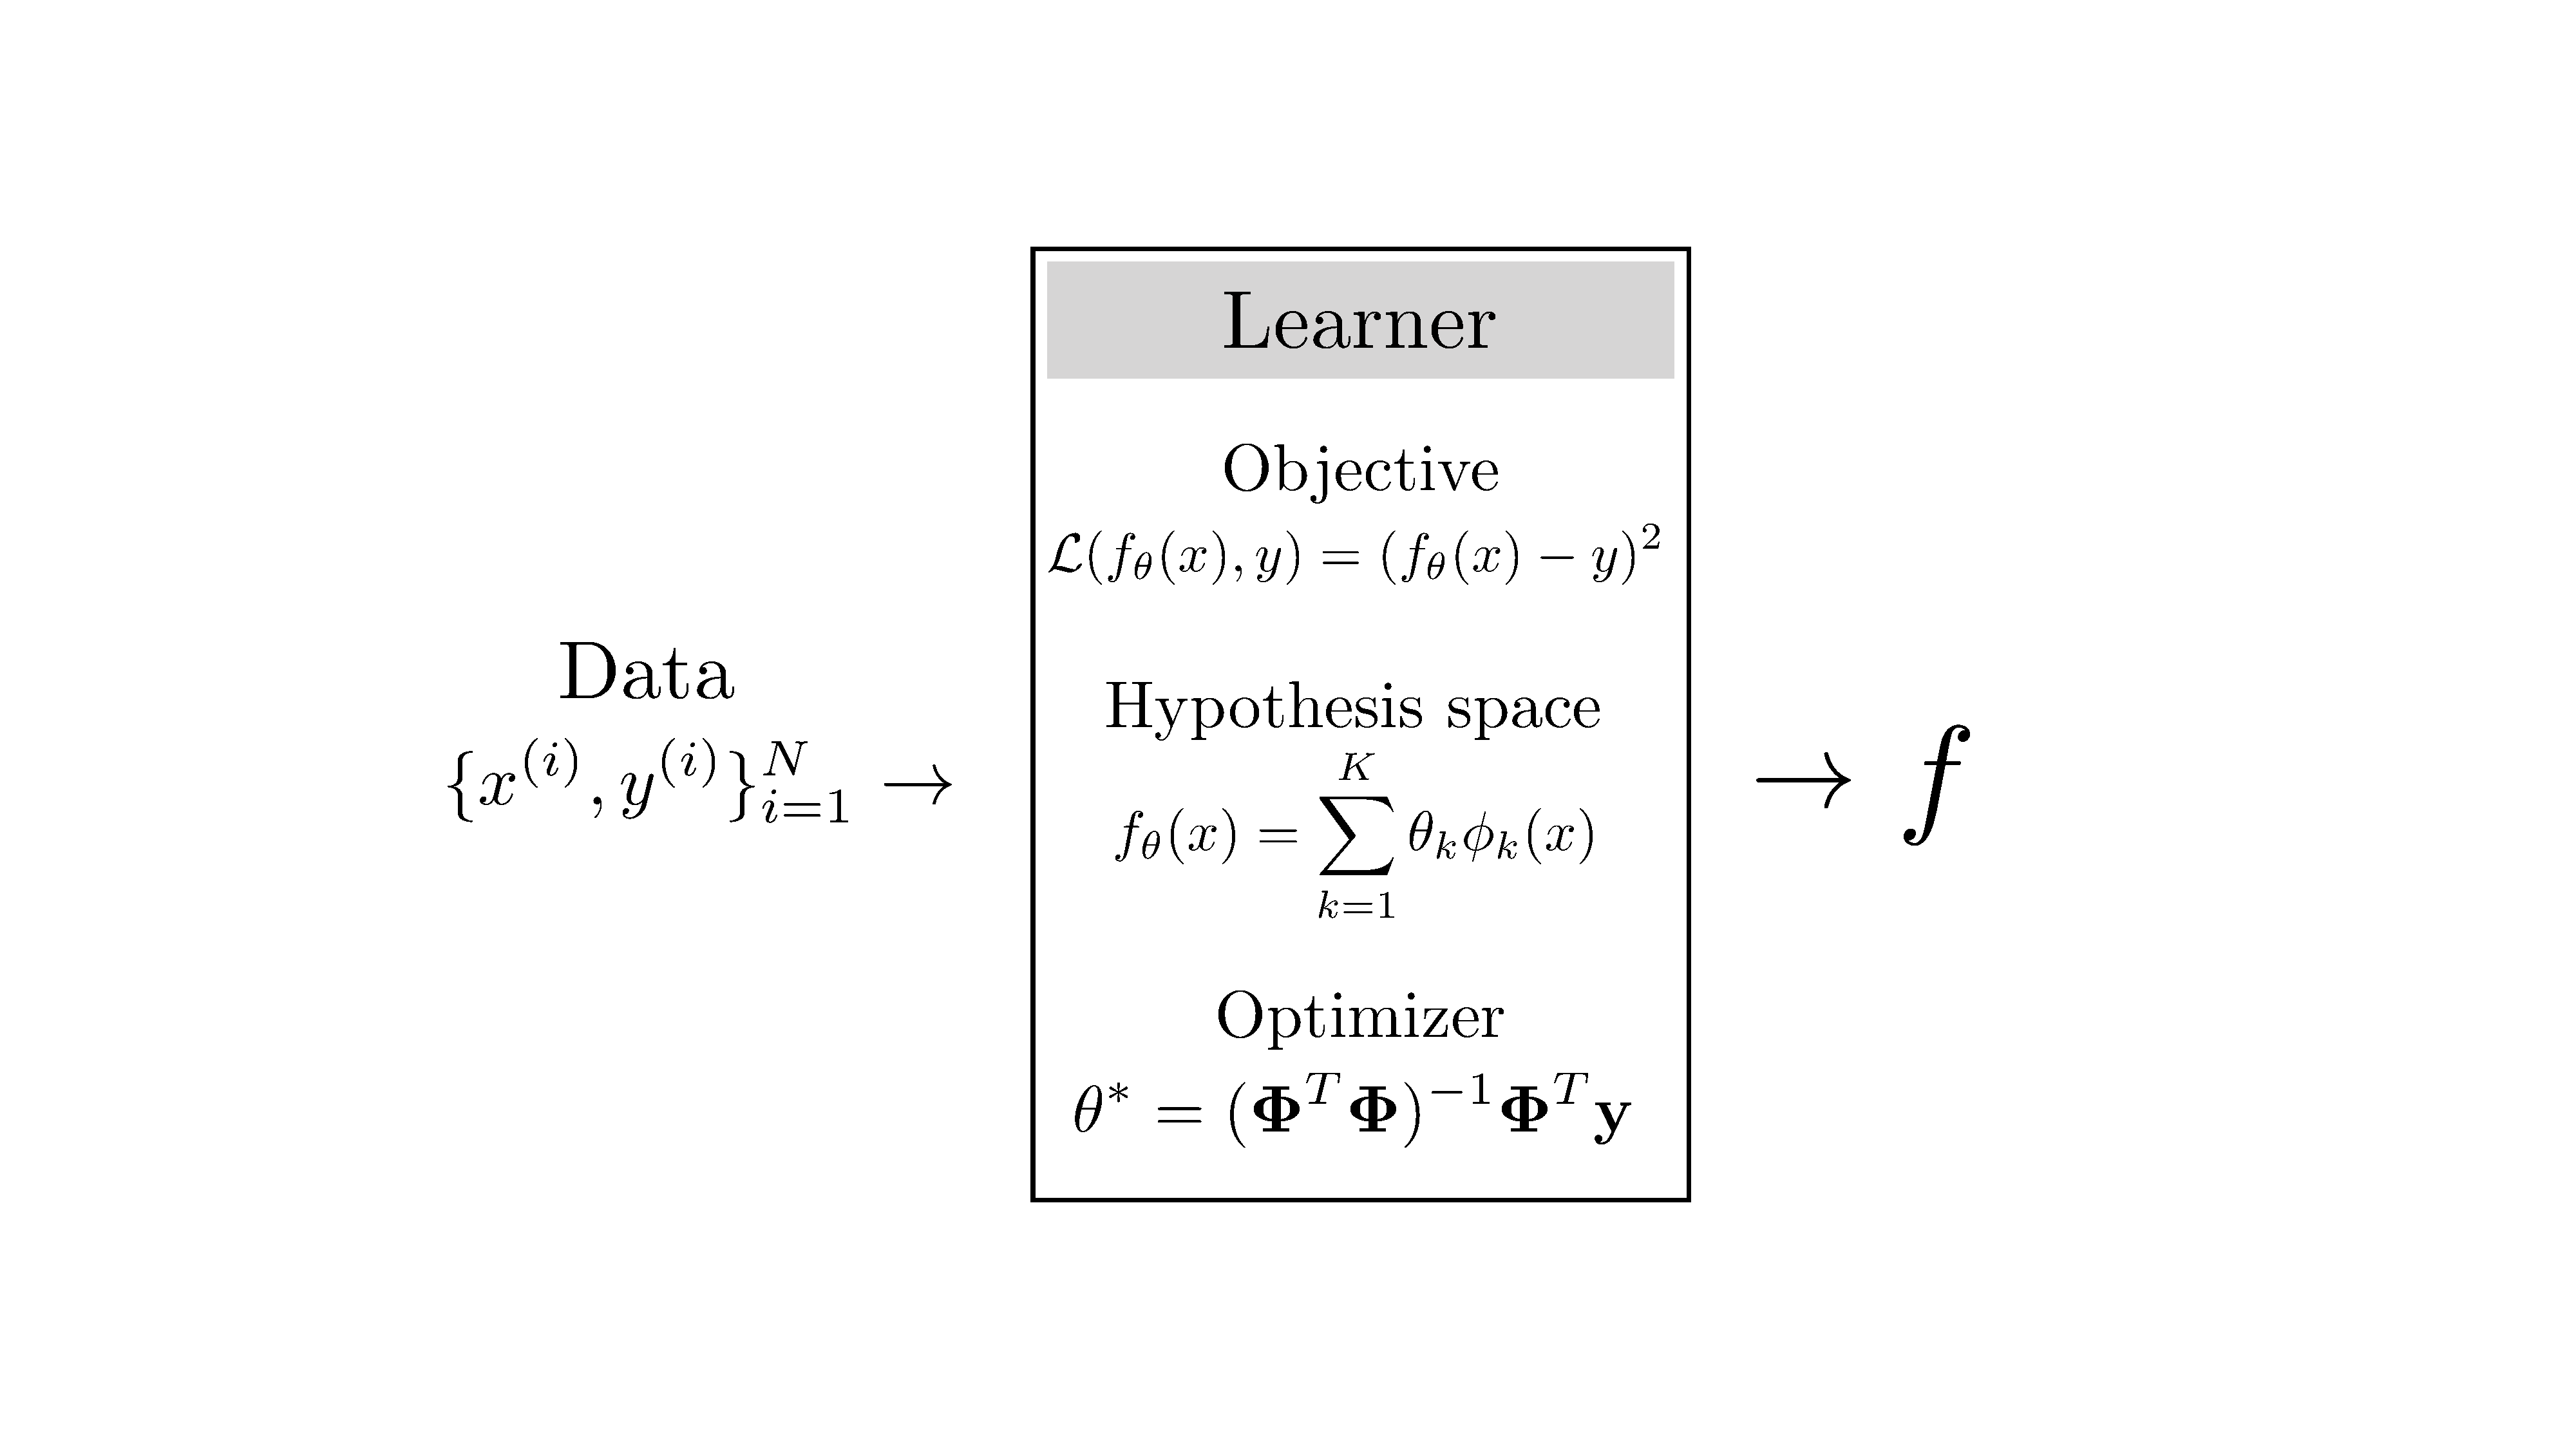
\includegraphics[width=0.65\linewidth]{./figures/problem_of_generalization/least_squares_polynomial_regression.pdf}
%     \label{fig:least_squares_polynomial_regression}
% \end{figure}

where
\begin{equation}
    \mathbf{\Phi} = 
     \begin{bmatrix}
        1 & x^{(1)} & x^{(1)^2} & ... & x^{(1)^K} \\
        1 & x^{(2)} & x^{(2)^2} & ... & x^{(2)^K} \\
        \vdots & \vdots & \vdots & \vdots & \vdots \\
        1 & x^{(N)} & x^{(N)^2} & ... & x^{(N)^K}  \\
    \end{bmatrix}
\end{equation}
\marginnote{This same trick works for any kind of function $\phi$, not just polynomials. The $\phi$ could be an expansion into a Fourier basis, for example. The general name for this kind of regression is {\bf basis function regression}; it is equivalent to linear regression on top of \textit{features} of $x$ (i.e., functions of $x$) rather than directly on $x$ itself.}[-6cm]

The matrix $\mathbf{\Phi}$ is an array of the features (columns) for each datapoint (rows). It plays the same role as data matrix $\mathbf{X}$ did in \chap{\ref{chapter:intro_to_learning}}; in fact we often call matrices of the feature representations of each datapoint also as a \textbf{data matrix}. As an exercise, you can derive the closed form of the optimizer, given above, using the same steps as we did for linear regression in \chap{\ref{chapter:intro_to_learning}}.\marginnote{When we get to the chapters on neural nets we will see that data matrices appear all over. A neural net is a sequence of transformations of an input data matrix into increasingly more powerful feature representations of the data, i.e. a sequence of better and better data matrices.}[-4.3cm]

\subsection{Polynomial Regression as a Lens into Generalization}
%To understand underfitting we measure it with {\bf approximation error}. The latter is called overfitting and we measure it with {\bf generalization error}.

What happens as we increase the order of the polynomial $K$, that is, we use $K+1$ basis functions $x^0, \ldots, x^K$? With $K=1$, we arrive back at linear regression. With $K=2$, we are fitting quadratic functions (i.e., parabolas) to the training data. As $K$ increases, the hypothesis space expands to include ever more curvy fits to the data, as shown in \fig{\ref{fig:under_and_overfitting}}.

\begin{figure}[h]
    \centerline{
    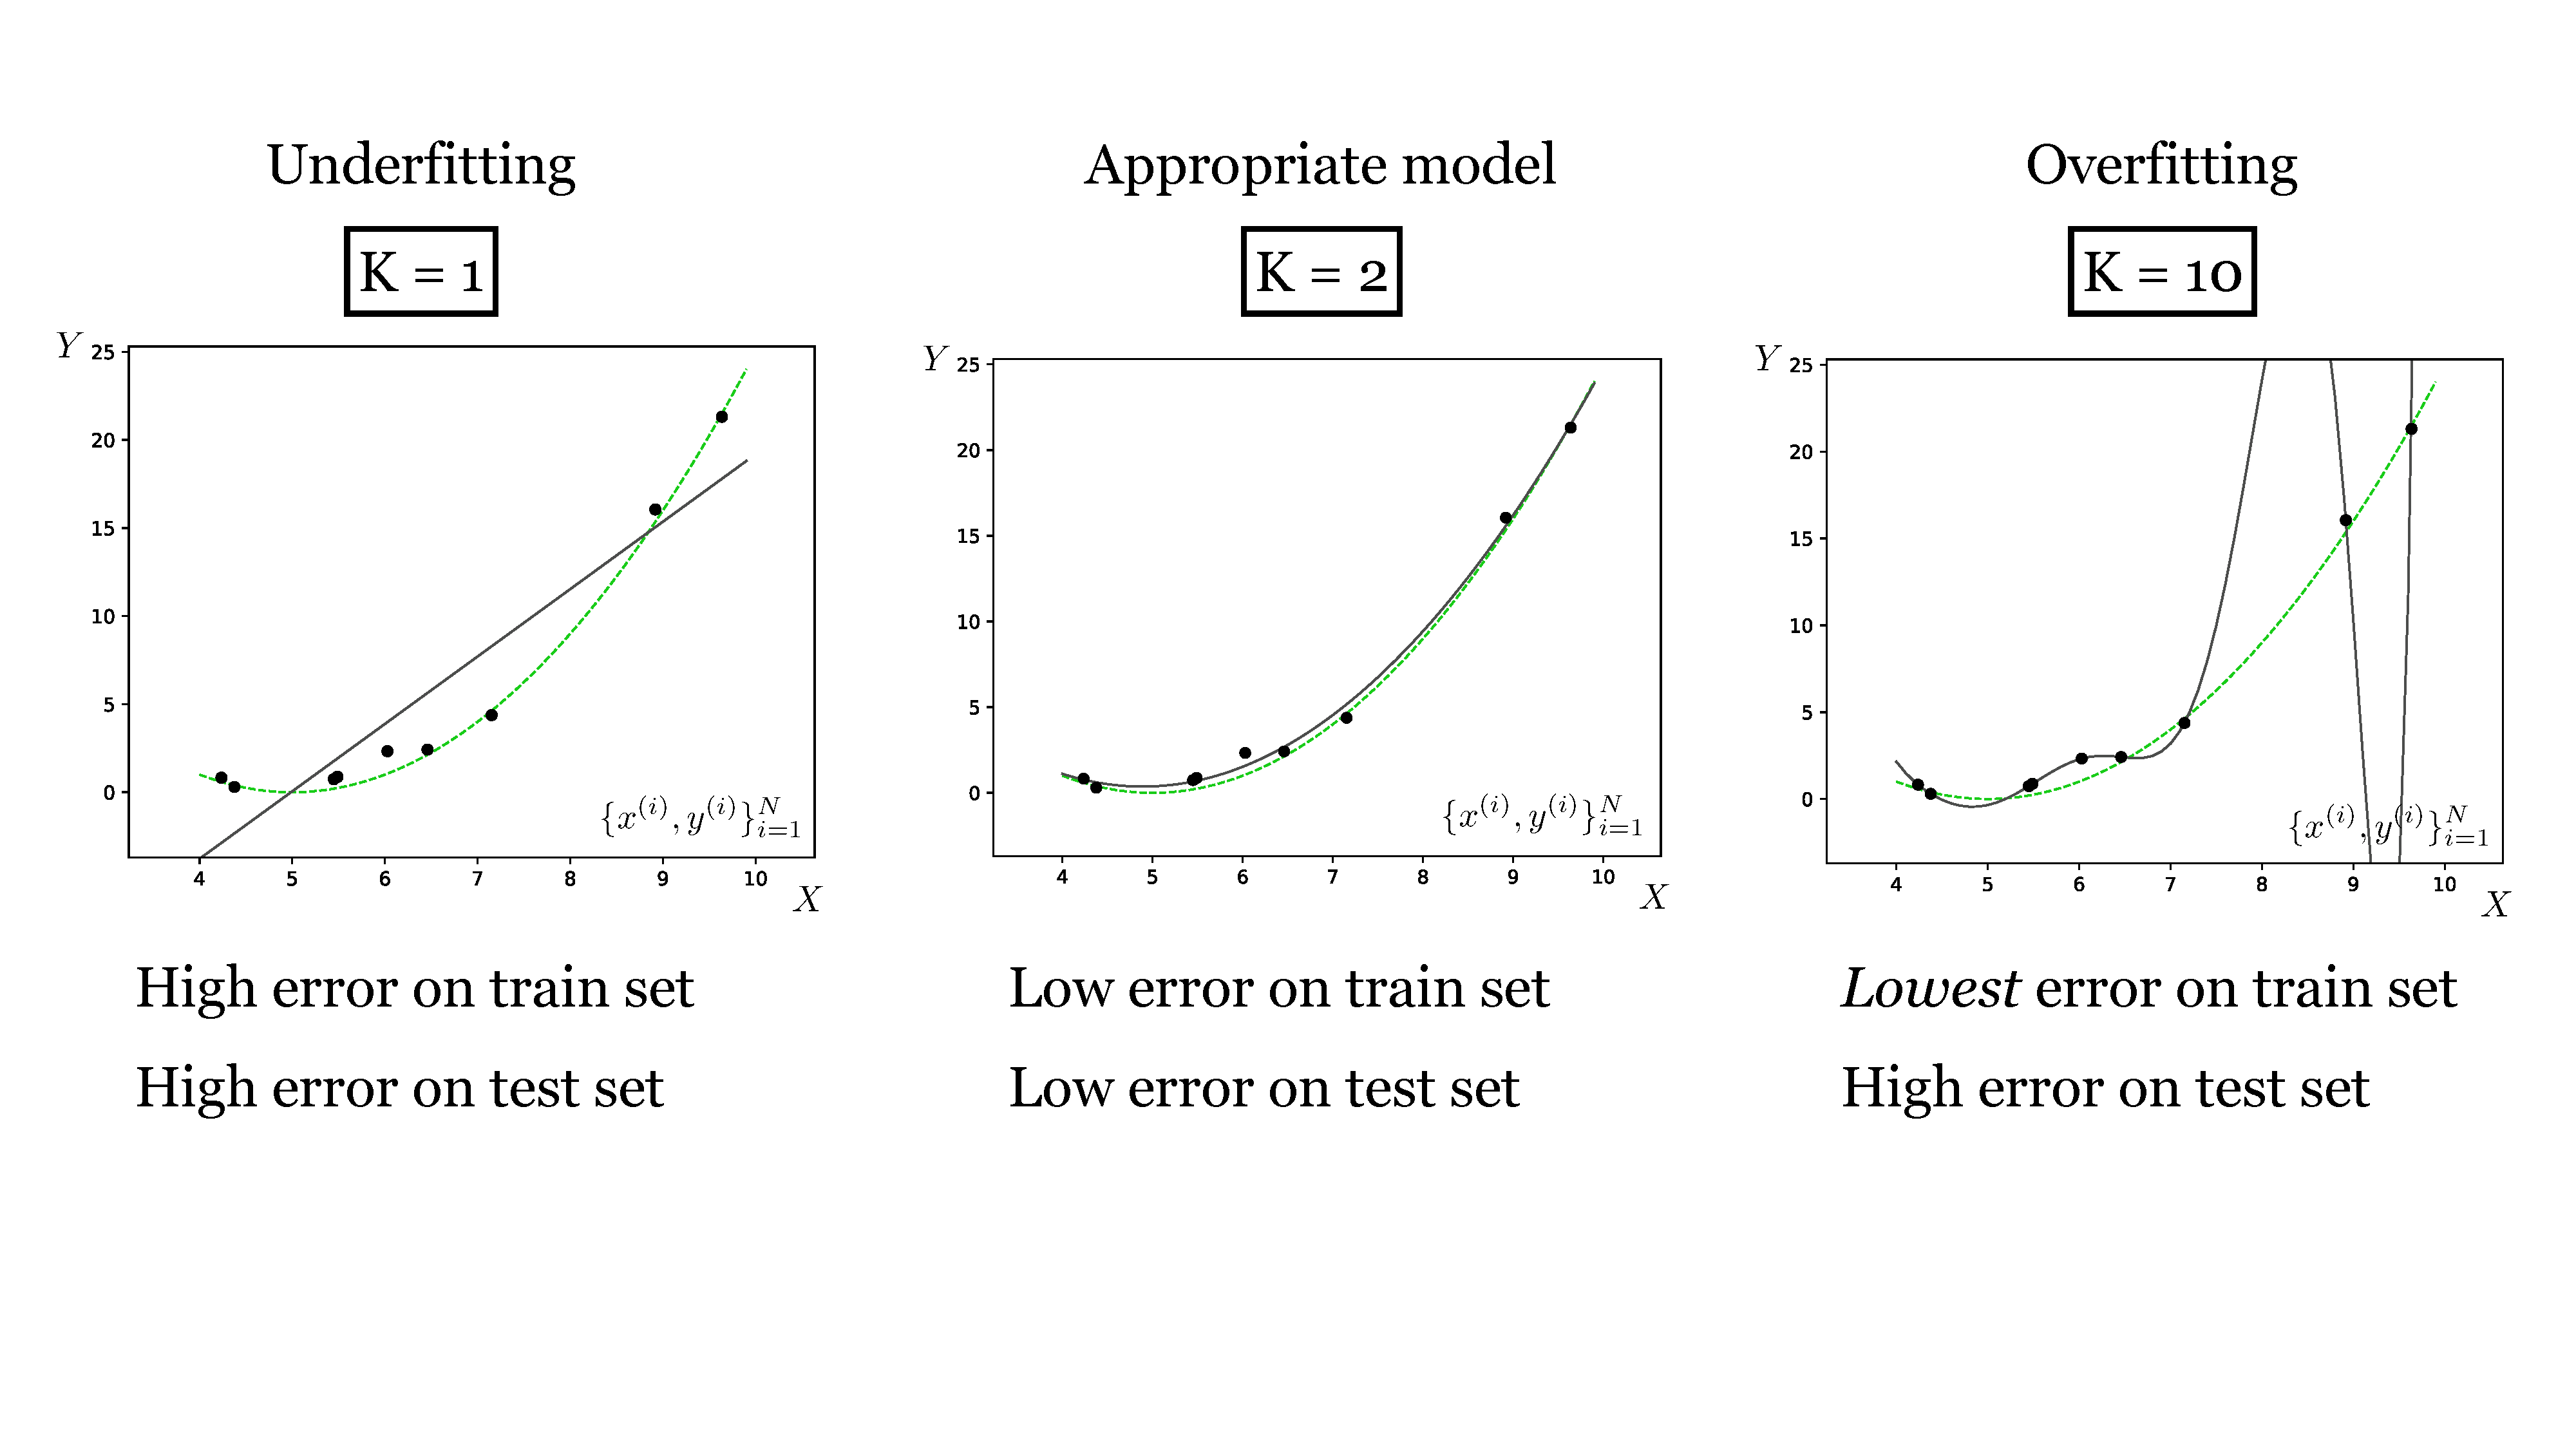
\includegraphics[width=1.0\linewidth]{./figures/problem_of_generalization/under_and_overfitting.pdf}
    }
    \caption{Underfitting and overfitting.}
    \label{fig:under_and_overfitting}
\end{figure}

The black line is the model's fit. The green line is the ground truth relationship between random variables $X$ and $Y$. The observed data $\{x^{(i)}, y^{(i)}\}_{i=1}^N$ is the black points, and this data is sampled from the green line plus observation noise. We refer to the full process that generates the data as the {\bf data generating process}:
\begin{align}
    Y &= X^2 + 1 &\triangleleft \quad\text{true underlying relationship}\\
    \epsilon &\sim \mathcal{N}(0,1) &\triangleleft \quad\text{observation noise}\\
    Y^\prime &= Y + \epsilon &\triangleleft \quad\text{noisy observations}\\
    x,y &\sim p(X,Y^{\prime}) &\triangleleft \quad\text{data-generating process}
\end{align}\marginnote{This data generating process assumes there is no noise in our observations of $x$. This is a common assumption in least-squares regression problems. Other models relax this assumption; for example, the generative models we will see in \chap{\ref{chapter:generative_models}} model uncertainty in both the $x$ and $y$ observations jointly.}[-3cm]
As we increase $K$ we fit the data points better and better, but eventually start \emph{overfitting}, where the model perfectly interpolates the data (passes through every datapoint) but deviates more and more from the true data-generating line. Why does that happen? It's because for $K=10$ the curve can become wiggly enough to not just fit the true underlying relationship but also to \textit{fit the noise}, the minor offsets $\epsilon$ around the green line. This noise is \textit{a property of the training data that does not generalize to the test data}; the test data will have different observation noise. That's what we mean when we say a model is overfitting.

As $K$ grows, a second phenomenon also occurs. For $K=10$ there are many hypotheses (polynomial functions) that perfectly the data (true function + noise) -- there is insufficient data for the objective to uniquely identify one of the hypotheses to be the best. Because of this, the hypothesis output by the optimizer may be an arbitrary one, or rather will be due to details of the optimization algorithm (e.g., how it is initialized), rather than selected by the objective. The optimizer we used above has a tendency to pick, among all the equally good hypotheses, one that is very curvy. This is an especially bad choice in this example, because the true function is much more smooth.

%So, overfitting can include two phenomena (both of which we see here): the model can be fitting noise (aspects of training data that don't generalize to test data) and the model might be underconstrained, having no unique minimizer to the objective, and therefore 

\index{Approximation error}{\bf Approximation error} is the gap between the black line and the training data points. Let $\{x_{(\texttt{train})}^{(i)}, y_{(\texttt{train})}^{(i)}\}_{i=1}^N$ be our training data set (the black points). Then the approximation error $J_{\texttt{approx}}$ is defined as the total cost incurred on this training data:
\begin{align}
    J_{\texttt{approx}} = \frac{1}{N} \sum_{i=1}^N \mathcal{L}(f_{\theta}(x_{(\texttt{train})}^{(i)}), y_{(\texttt{train})}^{(i)})
\end{align}
Notice that approximation error is the cost function we minimize in empirical risk minimization (\chap{\ref{chapter:intro_to_learning}}).

\index{Generalization error}{\bf Generalization error} is the gap between the black line and the green line, that is, the expected cost we would incur if we sampled a new test point at random from the true data generating process. Generalization error is often approximated by measuring performance on a heldout \index{Validation dataset}{\bf validation dataset}, $\{x_{(\texttt{val})}^{(i)}, y_{(\texttt{val})}^{(i)}\}_{i=1}^N$, which can simply be a subset of the data that we don't use for training or testing:
\begin{align}
    J_{\texttt{gen}} &= \mathbb{E}_{x,y \sim p_{\texttt{data}}} [ \mathcal{L}(f_{\theta}(x), y)]\\
                        &\approx \frac{1}{N} \sum_{i=1}^N \mathcal{L}(f_{\theta}(x_{(\texttt{val})}^{(i)}), y_{(\texttt{val})}^{(i)})
\end{align}

Approximation error goes down with increasing $K$ but all we really care about is generalization error, which measures how well we will do on test queries that are newly sampled from the true data generating process. For polynomial regression, generalization error obeys a U-shaped function with respect to $K$: at first it is high because we are underfitting; gradually we fit the data better and better and eventually we overfit, with generalization error becoming high again. \Fig{\ref{fig:under_and_overfitting_vs_polyK}} shows how it looks like for our example.
\begin{figure}[h]
    \centerline{
    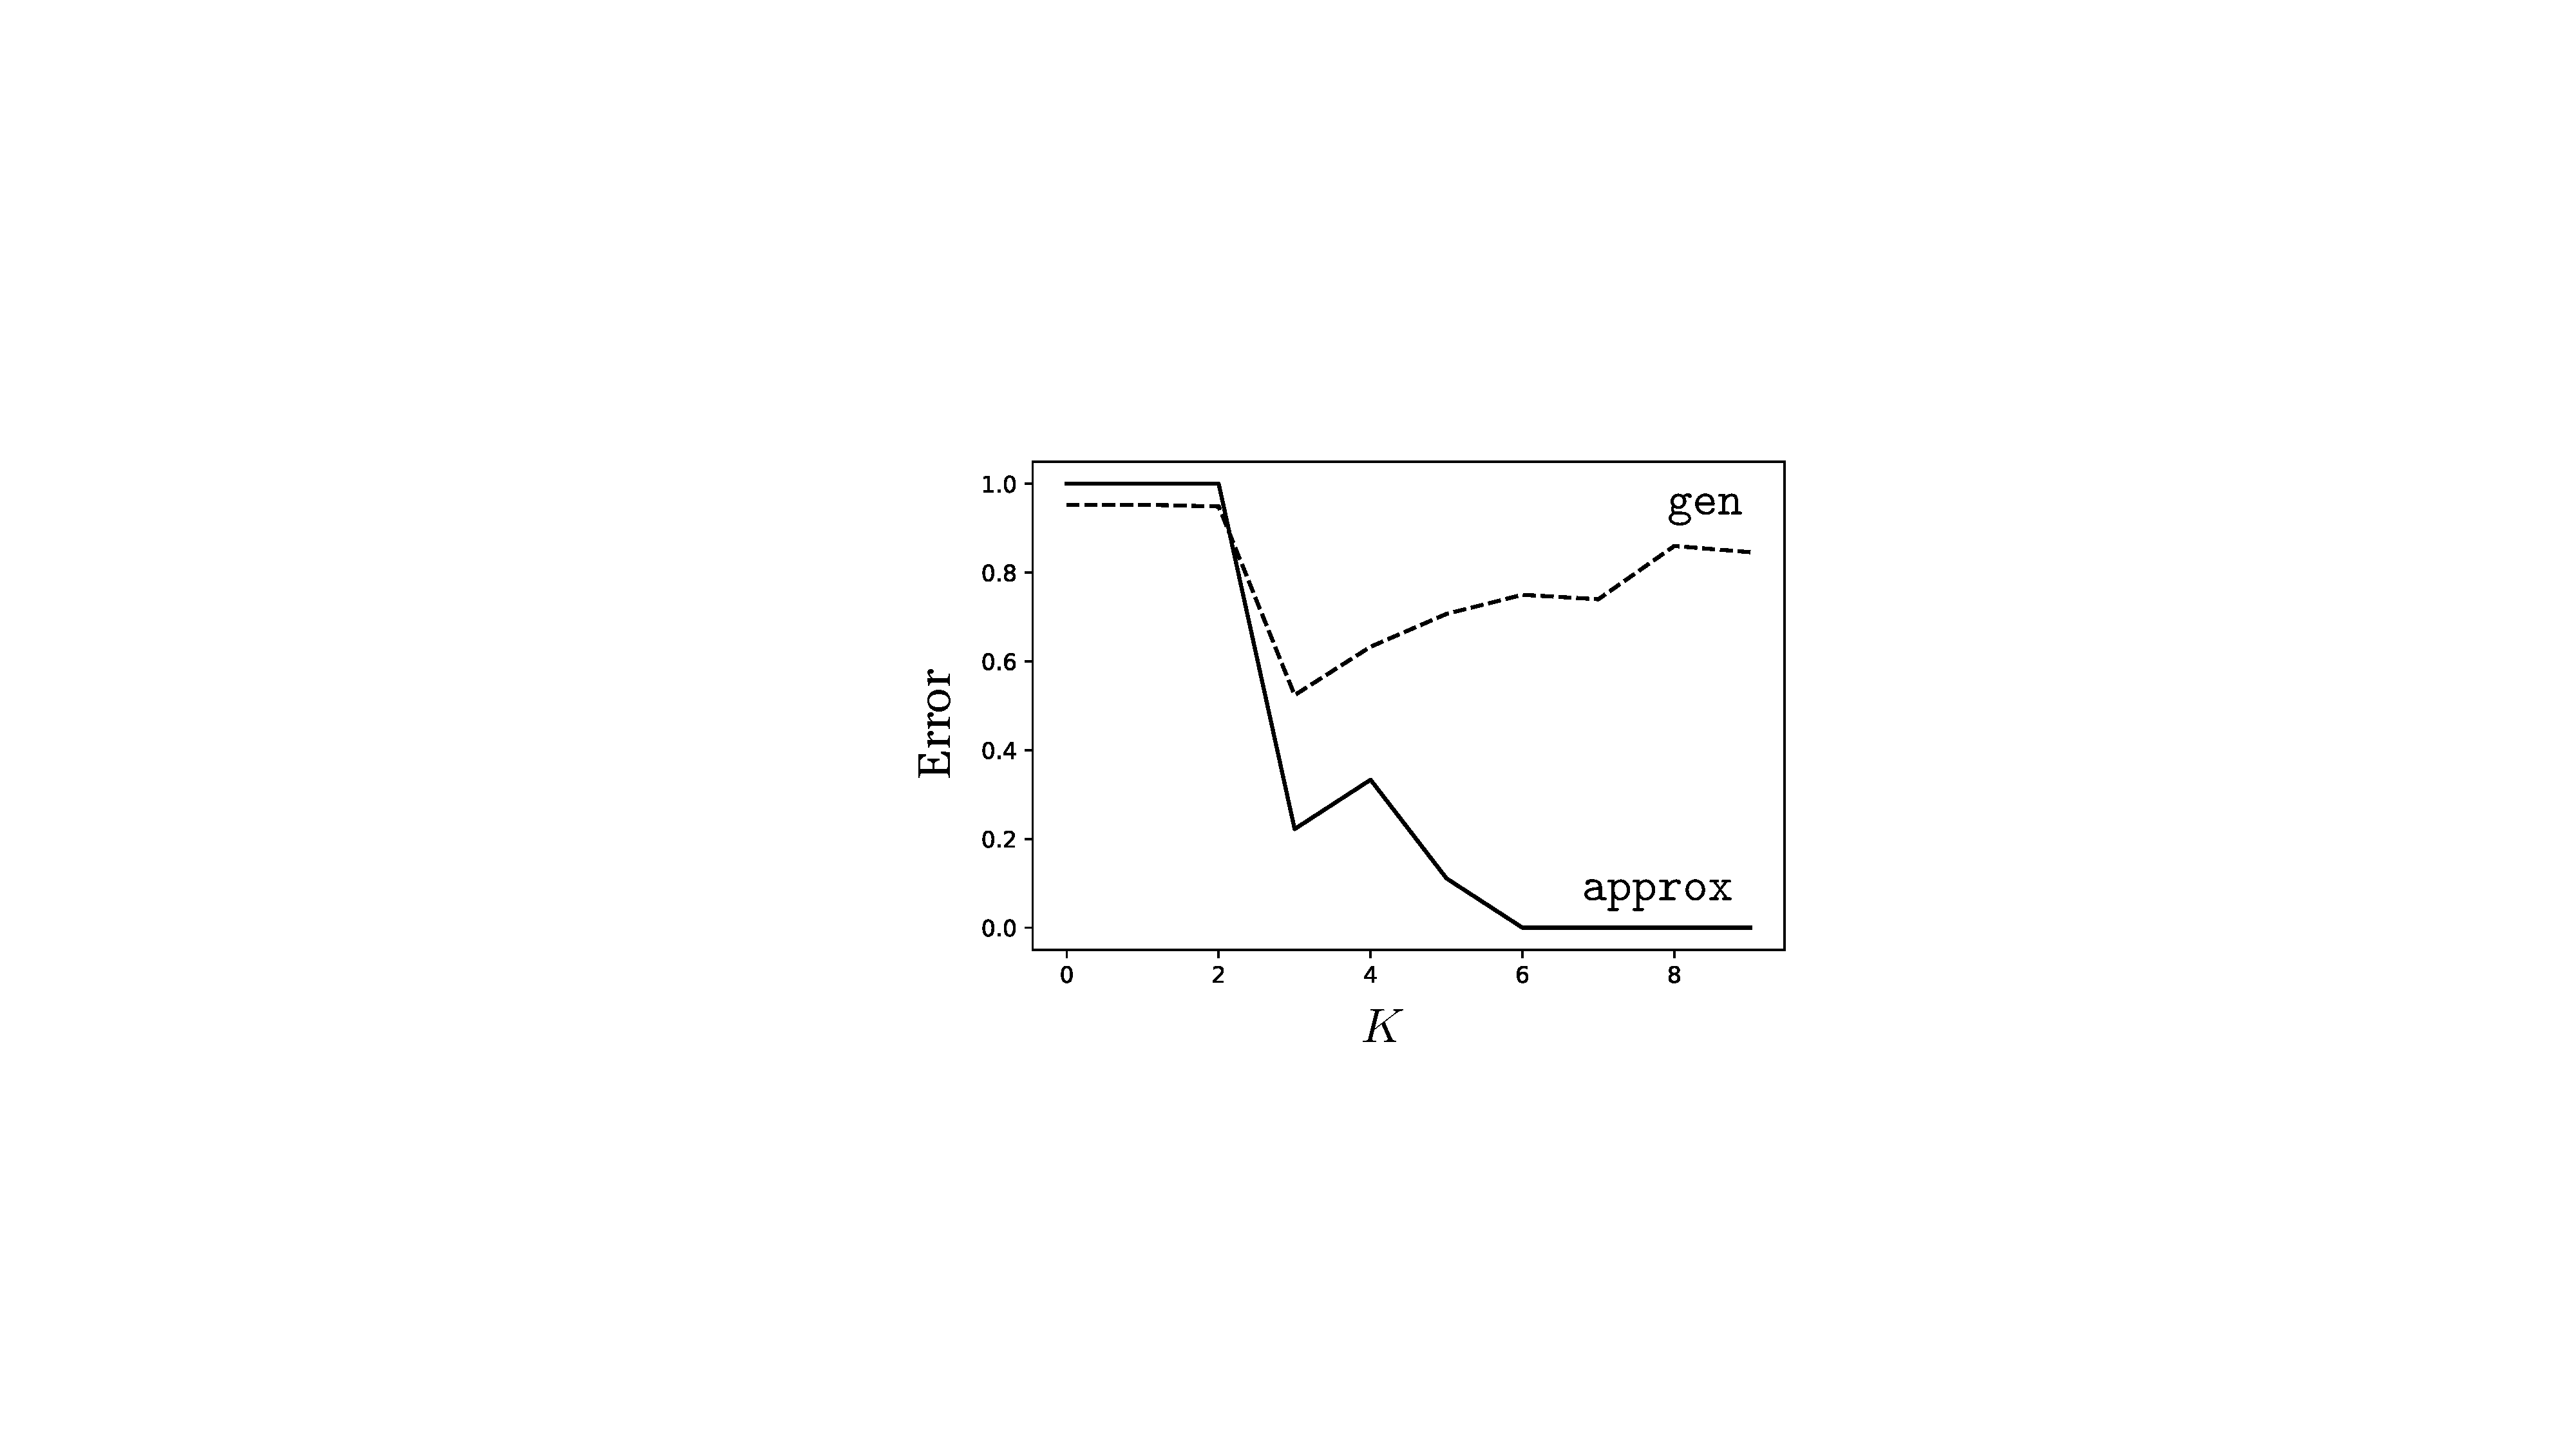
\includegraphics[width=0.48\linewidth]{./figures/problem_of_generalization/under_and_overfitting_vs_polyK.pdf}
    }
    \caption{Approximation error (\texttt{approx}) versus generalization error (\texttt{gen}) for polynomial regression of order $K$. Here we measured error as the proportion of validation points that are mispredicted (defined as having an $L_2$ prediction error greater than 0.25).}
    \label{fig:under_and_overfitting_vs_polyK}
\end{figure} %We use this notion of error since if we plotted the cost $J_{\texttt{gen}}$ as a function of $K$, for high values of $K$ the error becomes so large that the plot looks like a hockey stick and we only get to see one side of the U-shape.}[2.5cm]

This U-shaped curve is characteristic of classical learning regimes like polynomial regression, where we often find that the more parameters a model has, the more it will tend to overfit. However, this behavior does not well characterize modern learners like deep neural networks. Deep networks, which we will see in \chap{\ref{chapter:neural_nets}}, can indeed either underfit or overfit, but it is not the case that there is a simple relationship between the number of parameters the net has and whether that leads to underfitting versus overfitting. In fact, bigger deep nets with more parameters may overfit less than smaller nets. We discuss this further in \sect{\ref{sect:problem_of_generalization:rethinking_generalization}}. 

%\section{Bias-variance tradeoff}

%This idea can be formalized via the {\bf bias-variance tradeoff}.

%Show empirical plot from DLAICV. 

%An important concept in learning theory is {\bf model capacity}. 


\section{Regularization}

The previous example suggests a kind of ``Goldilocks principle.'' We should prefer hypotheses (functions $f$) that are sufficiently expressive to fit the data, but not so flexible that they can overfit the data. 


\index{Regularization}{\bf Regularization} refers to mechanisms that penalize function complexity so that we avoid learning too flexible a function that overfits. 
%Model capacity measures the expressivity of the hypothesis space. 
Typically, regularizers are terms we add to the objective that prefer simple functions in the hypothesis space, all else being equal. They therefore embody the principle of \index{Occam's razor}{\bf Occam's razor}. The general form of a regularized objective is:
\begin{align}
    J(\theta) = \overbrace{\frac{1}{N} \sum^N_{i=1} \mathcal{L}(f_{\theta}(x)^{(i)}, y^{(i)})}^\text{data fit loss} + \underbrace{\lambda R(\theta)}_\text{regularizer} \quad\quad\triangleleft \quad\text{regularized objective function} \label{eqn:problem_of_generalization:regularized_objective}
\end{align}
where $\lambda$ is a hyperparameter that controls the strength of the regularization.

One of the most common regularizers is to penalize the $L_p$ norm of the parameters of our model, $\theta$:
\begin{equation}
    R(\theta) = \norm{\theta}_{p}.
\end{equation}
\marginnote{The $L_p$-norm of $\mathbf{x}$ is $(\sum_i |x_i|^{p})^{\frac{1}{p}}$. The $L_2$-norm is the familiar least-squares objective.}[-0.4cm]
An especially common choice is $p=2$, in which case the regularizer is called \index{Ridge regression}{\bf ridge regularization} (which is also known as {\bf Tikonov regression}). In the context of neural networks, this regularizer is called \index{Weight decay}{\bf weight decay}. When $p=1$, the regularizer, applied to regression problems, is called \index{LASSO regression}{\bf LASSO regression}. For any $p$, the effect is to encourage most parameters to be zero, or near zero. When most parameters are zero, the function takes on a degenerate form, that is, a simpler form. For example, if we consider the quadratic hypothesis space $\theta_1 x + \theta_2 x^2$, then, if we use a strong $L_p$ regularizer, and if a linear fit is almost perfect, then $\theta_2$ will be forced to zero and the learned function will be linear rather than quadratic. Again, we find that regularization is an embodiment of Occam's razor: when multiple functions can explain the data, give preference to the simplest.

\subsection{Regularizers as Probabilistic Priors} Regularizers can be interpreted as \index{Priors}\textbf{priors} that prefer, a priori (before looking at the data), some solutions over others. Under this interpretation, the data fit loss (e.g., $L_2$ loss) is a likelihood function $p(\{y^{(i)}\}^N_{i=1} \given \{x^{(i)}\}^N_{i=1}, \theta)$ and the regularizer is a prior $p(\theta)$. Bayes' rule then states that the posterior $p(\theta \given \{x^{(i)}, y^{(i)}\}^N_{i=1})$ is proportional to the product of the prior and the likelihood. The log posterior is then the \textit{sum} of the log likelihood and the log prior, plus a constant. Hence we arrive at the form of \eqn{\ref{eqn:problem_of_generalization:regularized_objective}}.

\subsection{Revisiting the $\star$ Problem}\label{sec:problem_of_generalization:star_problem_revisited}
Remember the $\star$ problem from \chap{\ref{chapter:intro_to_learning}}?
\begin{align}
    3 \star 2 &= 36\nonumber \\
    7 \star 1 &= 49\nonumber \\
    5 \star 2 &= 100\nonumber \\
    2 \star 2 &= 16\nonumber
\end{align}
You may have figured out that $x \star y = (xy)^2$. We said that is the correct answer. But hold on, couldn't it be that $x \star y =  94.5x - 9.5x^2 + 4y^2 - 151$? That also perfectly explains these four examples (trust us, we checked). Or maybe $\star$ is the following Python program (\fig{\ref{fig:problem_of_generalization:python_star_solution}}).
\begin{figure}[h]
\begin{minipage}{1.0\linewidth}
\begin{minted}[xleftmargin=0.33\linewidth,xrightmargin=0.33\linewidth,
fontsize=\fontsize{8.5}{9},
frame=single,
framesep=2.5pt,
baselinestretch=1.05,
]{python}
def star(x,y):
    if x==2 && y==3:
        return 36
    elif x==7 && y==1:
        return 49
    elif x==5 && y==2:
        return 100
    elif x==2 && y==2:
        return 16
    else:
        return 0
\end{minted}
\end{minipage}
%}
\caption{A function written in Python that solves the $\star$ problem from \chap{\ref{chapter:intro_to_learning}}.}
\label{fig:problem_of_generalization:python_star_solution}
\end{figure}

That also perfectly fits the observed data. Why didn't you come up with those answers? What made $x \star y = (xy)^2$ more compelling?

We suspect your reason is again Occam's razor, which states that when multiple hypotheses equally well fit the data, you should prefer the simplest. To a human, it may be that $x \star y = (xy)^2$ is the simplest. To a computer, defining a proper notion of simplicity is a hard problem, but can be made precise.

As we saw, most regularizers can be given probabilistic interpretations as priors on the hypothesis, whereas the original objective (e.g., least-squares) measures the likelihood of the data given the hypothesis. These priors are not arbitrarily chosen. The notion of the {\bf Bayesian Occam's razor} derives such priors by noting that more complex hypothesis spaces must cover more possible hypotheses, and therefore must assign less prior mass to any single hypothesis (the prior probability of all possible hypotheses in the hypothesis space must sum to 1)~\cite{jefferys1992ockham, mackay2003information}. This is why, probabilistically, simpler hypotheses are more likely to be true.

\section{Rethinking Generalization} \label{sect:problem_of_generalization:rethinking_generalization}
A recent empirical finding is that some seemingly complex hypothesis spaces, such as deep nets (which we will see in later chapters), tend not to overfit, even though they have many more free parameters than the number of datapoints they are fit to. Exactly why this happens is an ongoing topic of research~\cite{zhang2016understanding}. But we should not be too surprised. The number of parameters is just a rough proxy for model capacity (i.e., the expressivity of the hypothesis space). A single parameter that has infinite numerical precision can parameterize an arbitrarily complex function. Such a parameter defines a very expressive hypothesis space and will be capable of overfitting data. Conversely, if we have a million parameters, but they are regularized so that almost all are zero, then these parameters may end up defining a simple class of functions, which does not overfit the data. So you can think of the number of parameters as a rough estimate of model capacity, but it is not at all the full story. See \cite{belkin2018reconciling} for more discussion on this point.%Overfitting is fundamentally related to \emph{model capacity}, not number of parameters, but often number of parameters is a good proxy. %Ideas from information theory can be used to define more appropriate measures of expressivity than ``number of parameters". %However, it has long been clear that overfitting is not really about \emph{number} of free parameters, rather the complexity of the hypothesis space. A function with many parameters tends to be more complex than a function with   

\section{Three Tools in the Search for Truth: Data, Priors, and Hypotheses}

In this section, we will introduce a perspective on learning and generalization that puts all our tools together. We will consider learning as akin to searching for the proverbial needle in a haystack. The haystack is our search space (i.e., the hypothesis space). The needle is the ``truth'' we are seeking, that is, the true function that generates our observations. 

We have several tools at our disposal to help us pinpoint the location of the needle, and in this section we will focus on the following three: \textit{data}, \textit{priors}, and \textit{hypotheses}. 

The first tool, \textit{data}, was the topic of \chap{\ref{chapter:intro_to_learning}}. In vision, the data is observations of the world like photos and videos. Finding explanations consistent with the observed data is the centerpiece of learning-based vision.

The second tool at our disposal was introduced earlier in this chapter: priors (a.k.a. regularizers) that prefer some solutions over others a priori. 

The last tool at our disposal is the set of \textit{hypotheses} under consideration for what the true function may be. The hypothesis space constrains which solutions we can possibly find. If the true solution is not in our hypothesis space, then no amount of data or priors can help us find it. This situation is like the old joke of a drunk man looking for his lost keys under a lamppost~\cite{freedman2010wrong}. ``Why are you looking there,'' a cop asks. ``Because this is where the light is.''

Together these three tools allow us to pinpoint one (or a few) good solutions in the space of all possibilities, as depicted in the cartoon in \fig{\ref{fig:problem_of_generalization:search_space_tools}}.
%\vspace{-0.3cm}

In this cartoon, we are learning a mapping from some domain $\mathcal{X}$ to another domain $\mathcal{Y}$. The hypothesis space, $\mathcal{F}$ (white circle; ``the lamppost's light'') places a hard constraint on the subset of possible mappings under consideration, the prior (yellow ellipse) places a soft constraint on which mappings are preferred over which others, and the data (green ellipse) also places a soft constraint on the space, preferring mappings that well fit the data. 

\begin{figure}[t]
    \centerline{
    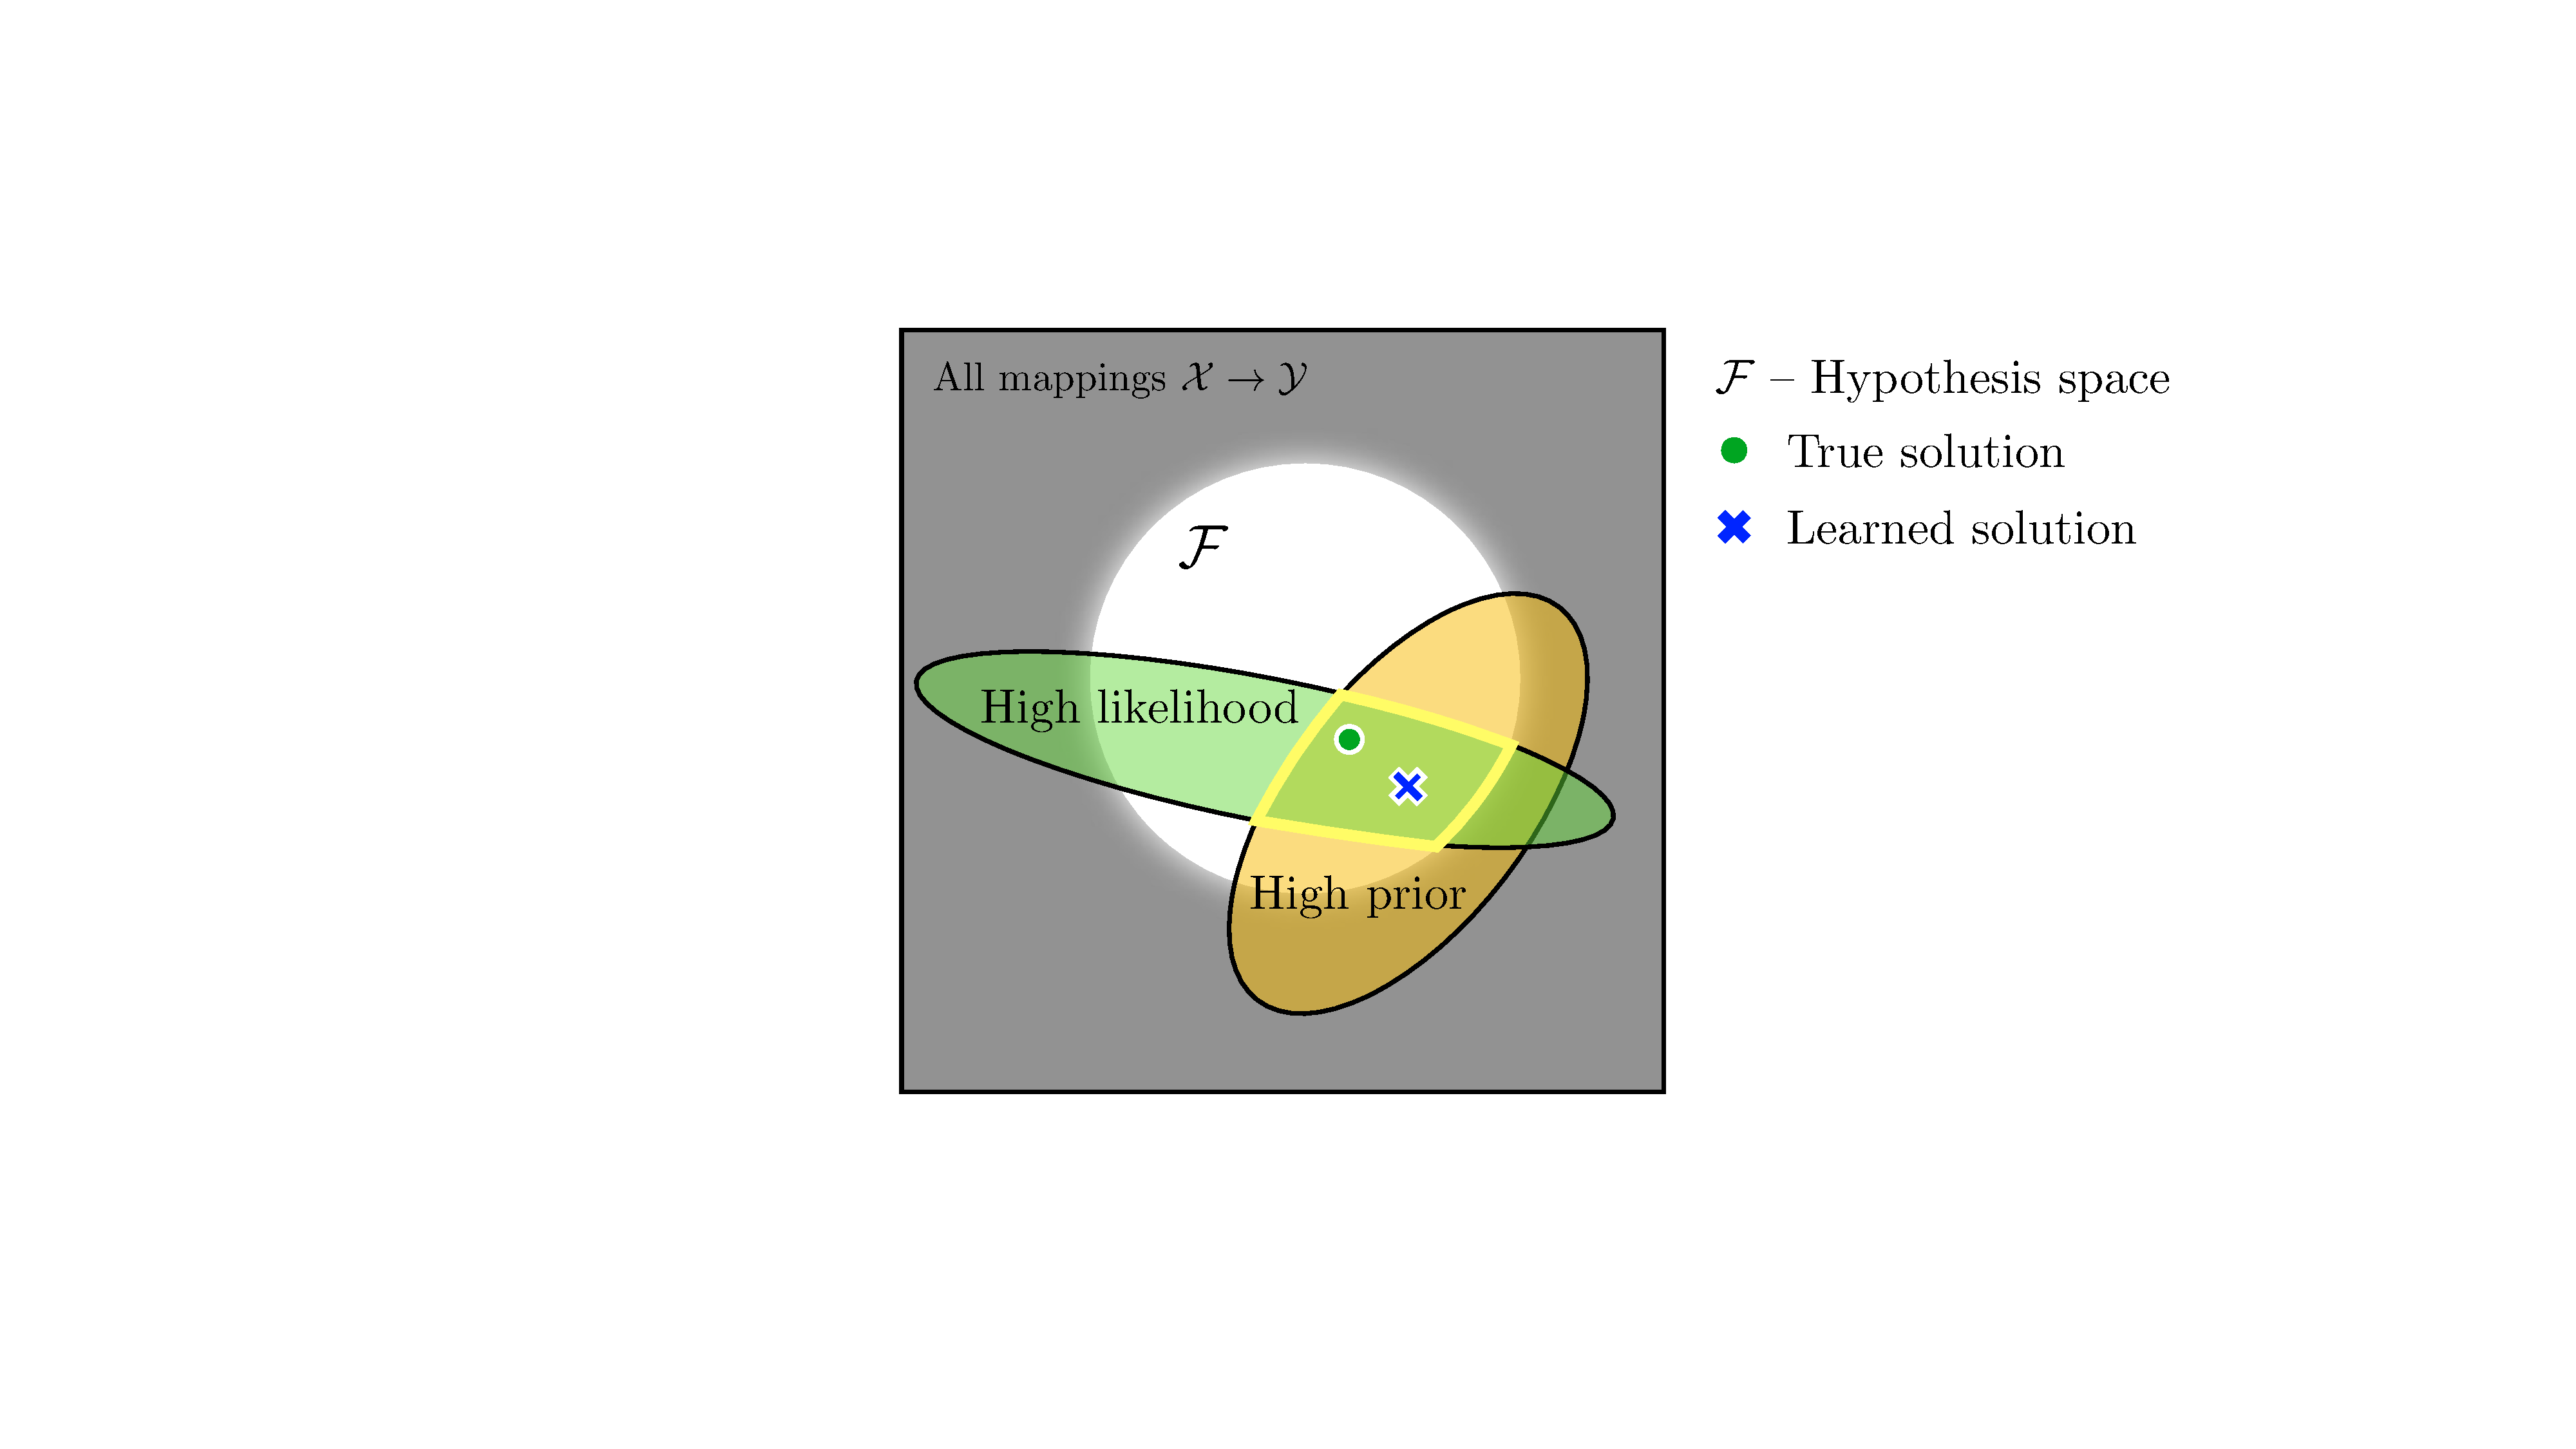
\includegraphics[width=0.65\linewidth]{./figures/problem_of_generalization/search_space_tools.pdf}
    }
    \caption{A cartoon of the tools for honing in on the truth.}
    \label{fig:problem_of_generalization:search_space_tools}
\end{figure}


Approximation error is low within the green region. If we didn't care about generalization, then it would be sufficient just to select any solution in this green region. But since we do care about generalization, we bias our picks toward the yellow region, which corresponds to a prior that selects points we believe to be closer to the true solution, even if they might not fit the data perfectly well. These tools isolate the area outlined in bright yellow as the region where we may find our needle of truth. A learning algorithm, which searches over $\mathcal{F}$ in order to maximize the likelihood times the prior, will find a solution somewhere in this outlined region. %The found solution will not necessarily coincide with the true solution but cannot be too far off, as long as the yellow outlined region indeed contains the truth. %will hopefully be nearby; if we shrink the yellow outlined region then we can be force the learner to get ever closer to the truth. 
%But it might not find the exact location of the true solution as the intersection of all our tools did not identify a unique solution in this example.

In the next three sections, we will explore these three tools in more detail through the simple experiment of fitting a curve to a set of datapoints.


\subsection{Experiment 1: Effect of Data}

Training data is the main source of information for a learner, and a learner is just like a detective: as it observes more and more data, it gets more and more evidence to narrow in on the solution. Here we will look at how data shapes the objective function $J$ for the following empirical risk minimization problem:
\begin{align}
    J(\theta; \{x^{(i)}, y^{(i)}\}^N_{i=1}) &= \frac{1}{N}\sum_i \lvert f_{\theta}(x^{(i)}) - y^{(i)}\rvert^{0.25} \quad\quad \triangleleft \quad\text{objective}\label{eqn:problem_of_generalization:error_fn_1}\\
    f_{\theta}(x) &= \theta_0 x + \theta_1 \sin(x)  \quad\quad \triangleleft \quad\text{hypothesis space}
\end{align}\marginnote{We use the exponent $0.25$, rather than the more common squared error, just so that the plots in \fig{\ref{fig:problem_of_generalization:more_data_more_constraints}} show more clearly the linear constraints (the dark lines) added by each datapoint to the objective $J$.}[-1.6cm]
In \fig{\ref{fig:problem_of_generalization:more_data_more_constraints}}, bottom row, we plot $J$ as a heatmap over the values obtained for different settings of $\theta$. On the top row we plot the data being fit, $\{x^{(i)}, y^{(i)}\}^N_{i=1}$, along with the function $f_{\theta}$ that achieves the best fit, and a sample other settings of $\theta$ that achieve within 0.1 of the cost of the best fit. Each column corresponds to some amount of training data $N$. Moving to the right, we increase $N$.

\begin{figure}[t]
    \centerline{
    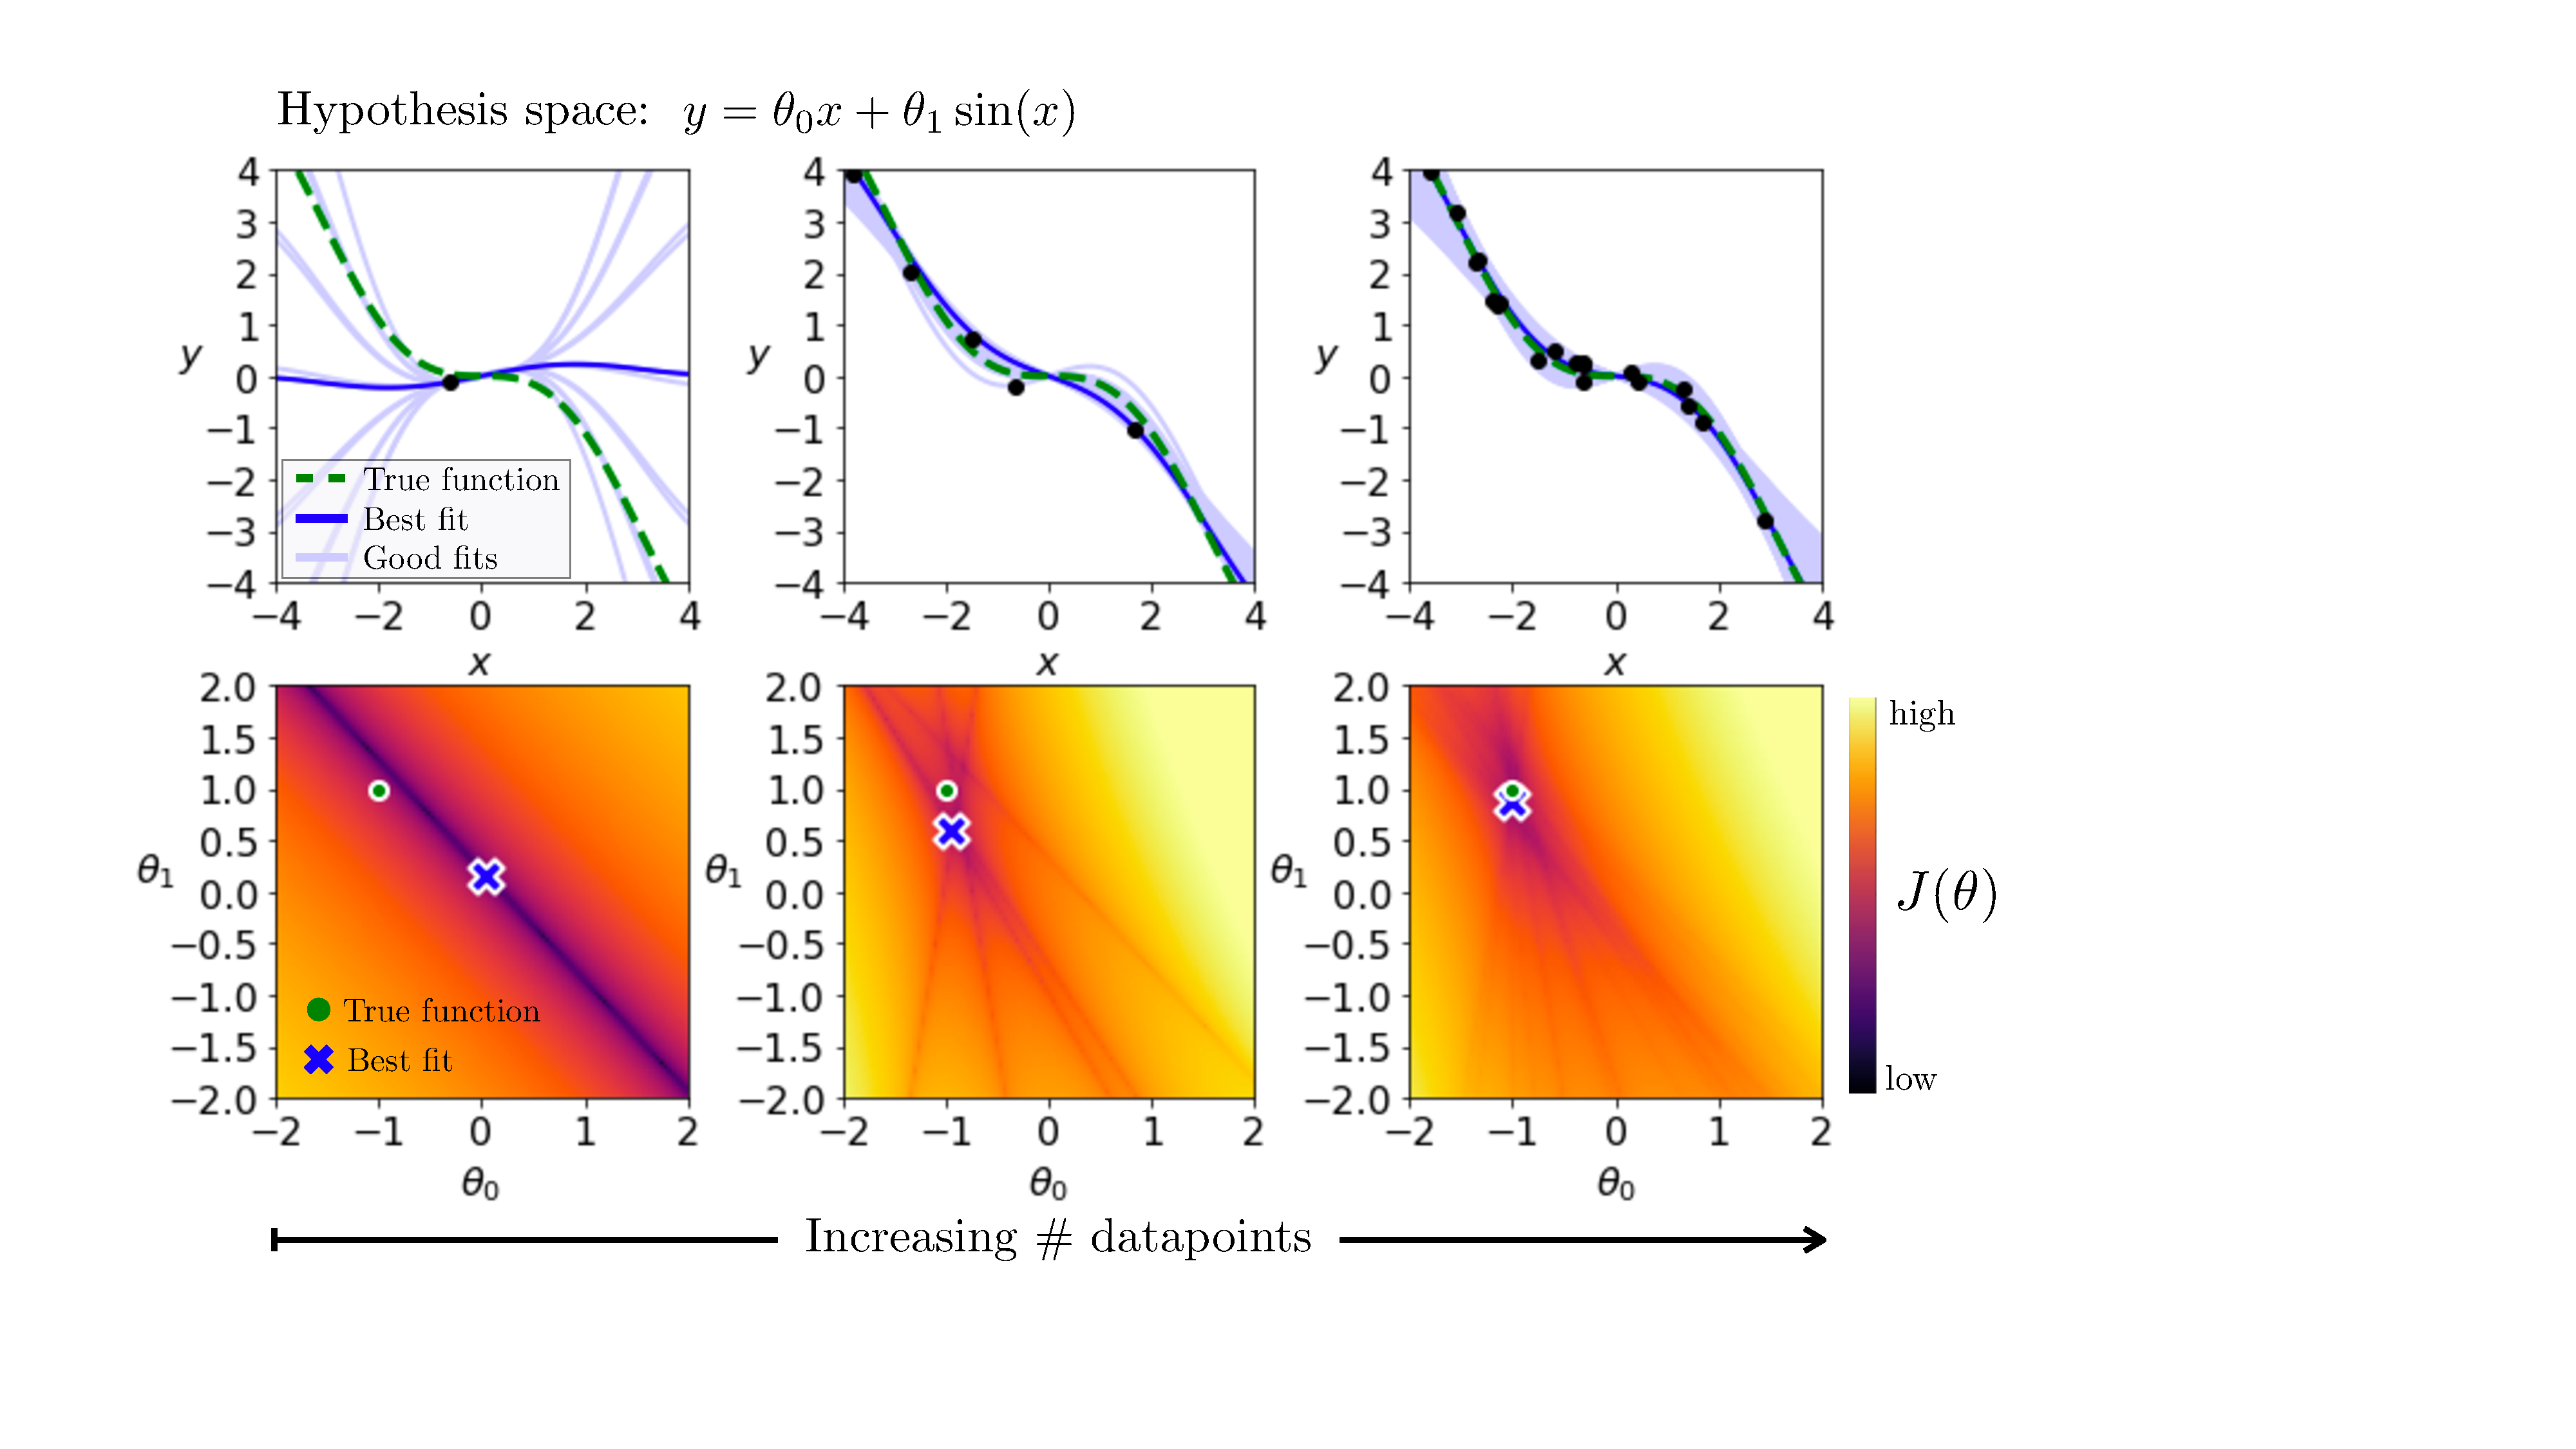
\includegraphics[width=1.0\linewidth]{./figures/problem_of_generalization/more_data_more_constraints.pdf}
    }
    \caption{More data, more (soft) constraints.}
    \label{fig:problem_of_generalization:more_data_more_constraints}
\end{figure}
\marginnote{The heatmaps here are reminiscent of a classic computer vision algorithm called the Hough transform~\cite{hough1959machine,duda1972use}. This transform can be used to find geometric primitives that fit feature points in images. In fact, the bottom row is \textit{exactly} the generalized Hough transform~\cite{duda1972use} of the data points in the top row, using $\theta_0 x + \theta_1 \sin(x)$ as the family of geometric primitives we are fitting.}[-9cm]

The first thing to look at is the leftmost column, where $N=1$. For a single datapoint, there are an infinite number of functions in our hypothesis space that perfectly fit that point. This shows up in the heatmaps as a \textit{line} of settings of $\theta$ that all achieve zero loss.\marginnote{Why a line? Because we have \textit{two} free parameters, $[\theta_0, \theta_1]$, and \textit{one} constraint, $y^{(1)} = \theta_0 x^{(1)} + \theta_1 \sin(x^{(1)})$, so we have one more parameter than constraint yielding a one-dimensional (1D) subspace of solutions.}[-0.4cm] The learning algorithm we used in this example picks a random solution from the set of solutions that achieve zero loss. Unfortunately, here it got unlucky and picked a solution that happens to be far from the true solution.

Next, look at the second column where we have $N=5$ training points. Ideally we want to find a curve that exactly passes through each point. Each \textit{single} datapoint adds one constraint to this problem, and each constraint shows up as a line in the heatmap for $J$ [the line of solutions that satisfy the constraint $y^{(i)} = \theta_0 x^{(i)} + \theta_1 \sin(x^{(i)})$ for that datapoint $i$]. The \textit{intersection} of all these constraints pinpoints the setting of parameters that fits \textit{all} that data. In this example, with five datapoints, there is no location where all the constraint lines intersect, which means there is no curve in our hypothesis space that can perfectly fit this data. Instead we settle for the curve that best approximates the data, according to our loss function. Notice that the learned solution is now pretty close to the true function that generated the data. It is not an exact match, because the data is generated by taking \textit{noisy} samples from the true data generating function.

Finally, let's look at the third column, where we are fitting 20 datapoints. Now the intersection (or, more precisely, average) of the losses for all the datapoints gives a relatively smooth cost function $J(\theta)$, and the learned solution is almost right on top of the true solution. This illustrates a very important point:
\begin{center}
    \textit{The more data you have, the less you need other modeling tools.}
\end{center}%\marginnote{As long as 1) the truth is within the hypothesis space, 2) the noise level is finite, and 3) what you care about is inferring truth.}

With enough data, the true solution will be pinpointed by data alone. However, when we don't have enough data, or when the data is noisy or incorrectly labeled, we can turn to our two other tools, which we will see next.
% processing is too expensive

%This point has several implications that are good to keep in mind. First, generally, the more data you have the better. Second, the more data you have, the less you need other tools to identify the truth -- if you have enough data you don't need regularizers or constraints. Third, because data scale tends to increase over time (we have more and can process more), you should expect that whatever architecture/regularizers are used in year $X$, a less constrained architecture with less regularized will be preferred in year $Y$, for $Y>X$. This is a rule of thumb that has been borne time and again: whatever \textit{inference} methods you learn in this book (meaning optimizers, features, objectives, architectures, models, etc), expect that fewer and fewer of them will be relevant in each subsequent year. Not because new methods will come along that make the current ones out of date (yes that will happen too) but because fewer and fewer methods are useful as data and compute scale. In some year $Z$ we will have enough data and compute that very ``naive'' methods are just as effective as the most sophisticated present approaches. This idea has been called ``the bitter lesson'' and it's good to get comfortable with it now so that you won't have a bitter surprise in a few years. 


\subsection{Experiment 2: Effect of Priors}

Now we will run a similar experiment to look at the effect of priors. In this experiment we will use a slightly different hypothesis space and objective function, namely
\begin{align}
    J(\theta; \{x^{(i)}, y^{(i)}\}^N_{i=1}) &= \frac{1}{N}\sum_i \norm{f_{\theta}(x^{(i)}) - y^{(i)}}_2^2 + \lambda \norm{\theta}_2^2 \quad\quad \triangleleft \quad\text{objective}\\
    f_{\theta}(x) &= \theta_0 x + \theta_1 x \quad\quad \triangleleft \quad\text{hypothesis space}
\end{align}
We will look at the effect of the ridge regularizer $\norm{\theta}_2^2$. We plot the energy landscape and function fit for this problem in \fig{\ref{fig:problem_of_generalization:more_regularizer_more_constraints}}, fitting to a single datapoint. The ridge regularizer prefers solutions with small parameter norm, so its contribution to the energy landscape is to place a quadratic bowl around the origin. As we increase $\lambda$ (moving left to right in the subplots), the effect of the regularizer becomes stronger and pulls the learned solution closer and closer to the origin.

\begin{figure}[t]
    \centerline{
    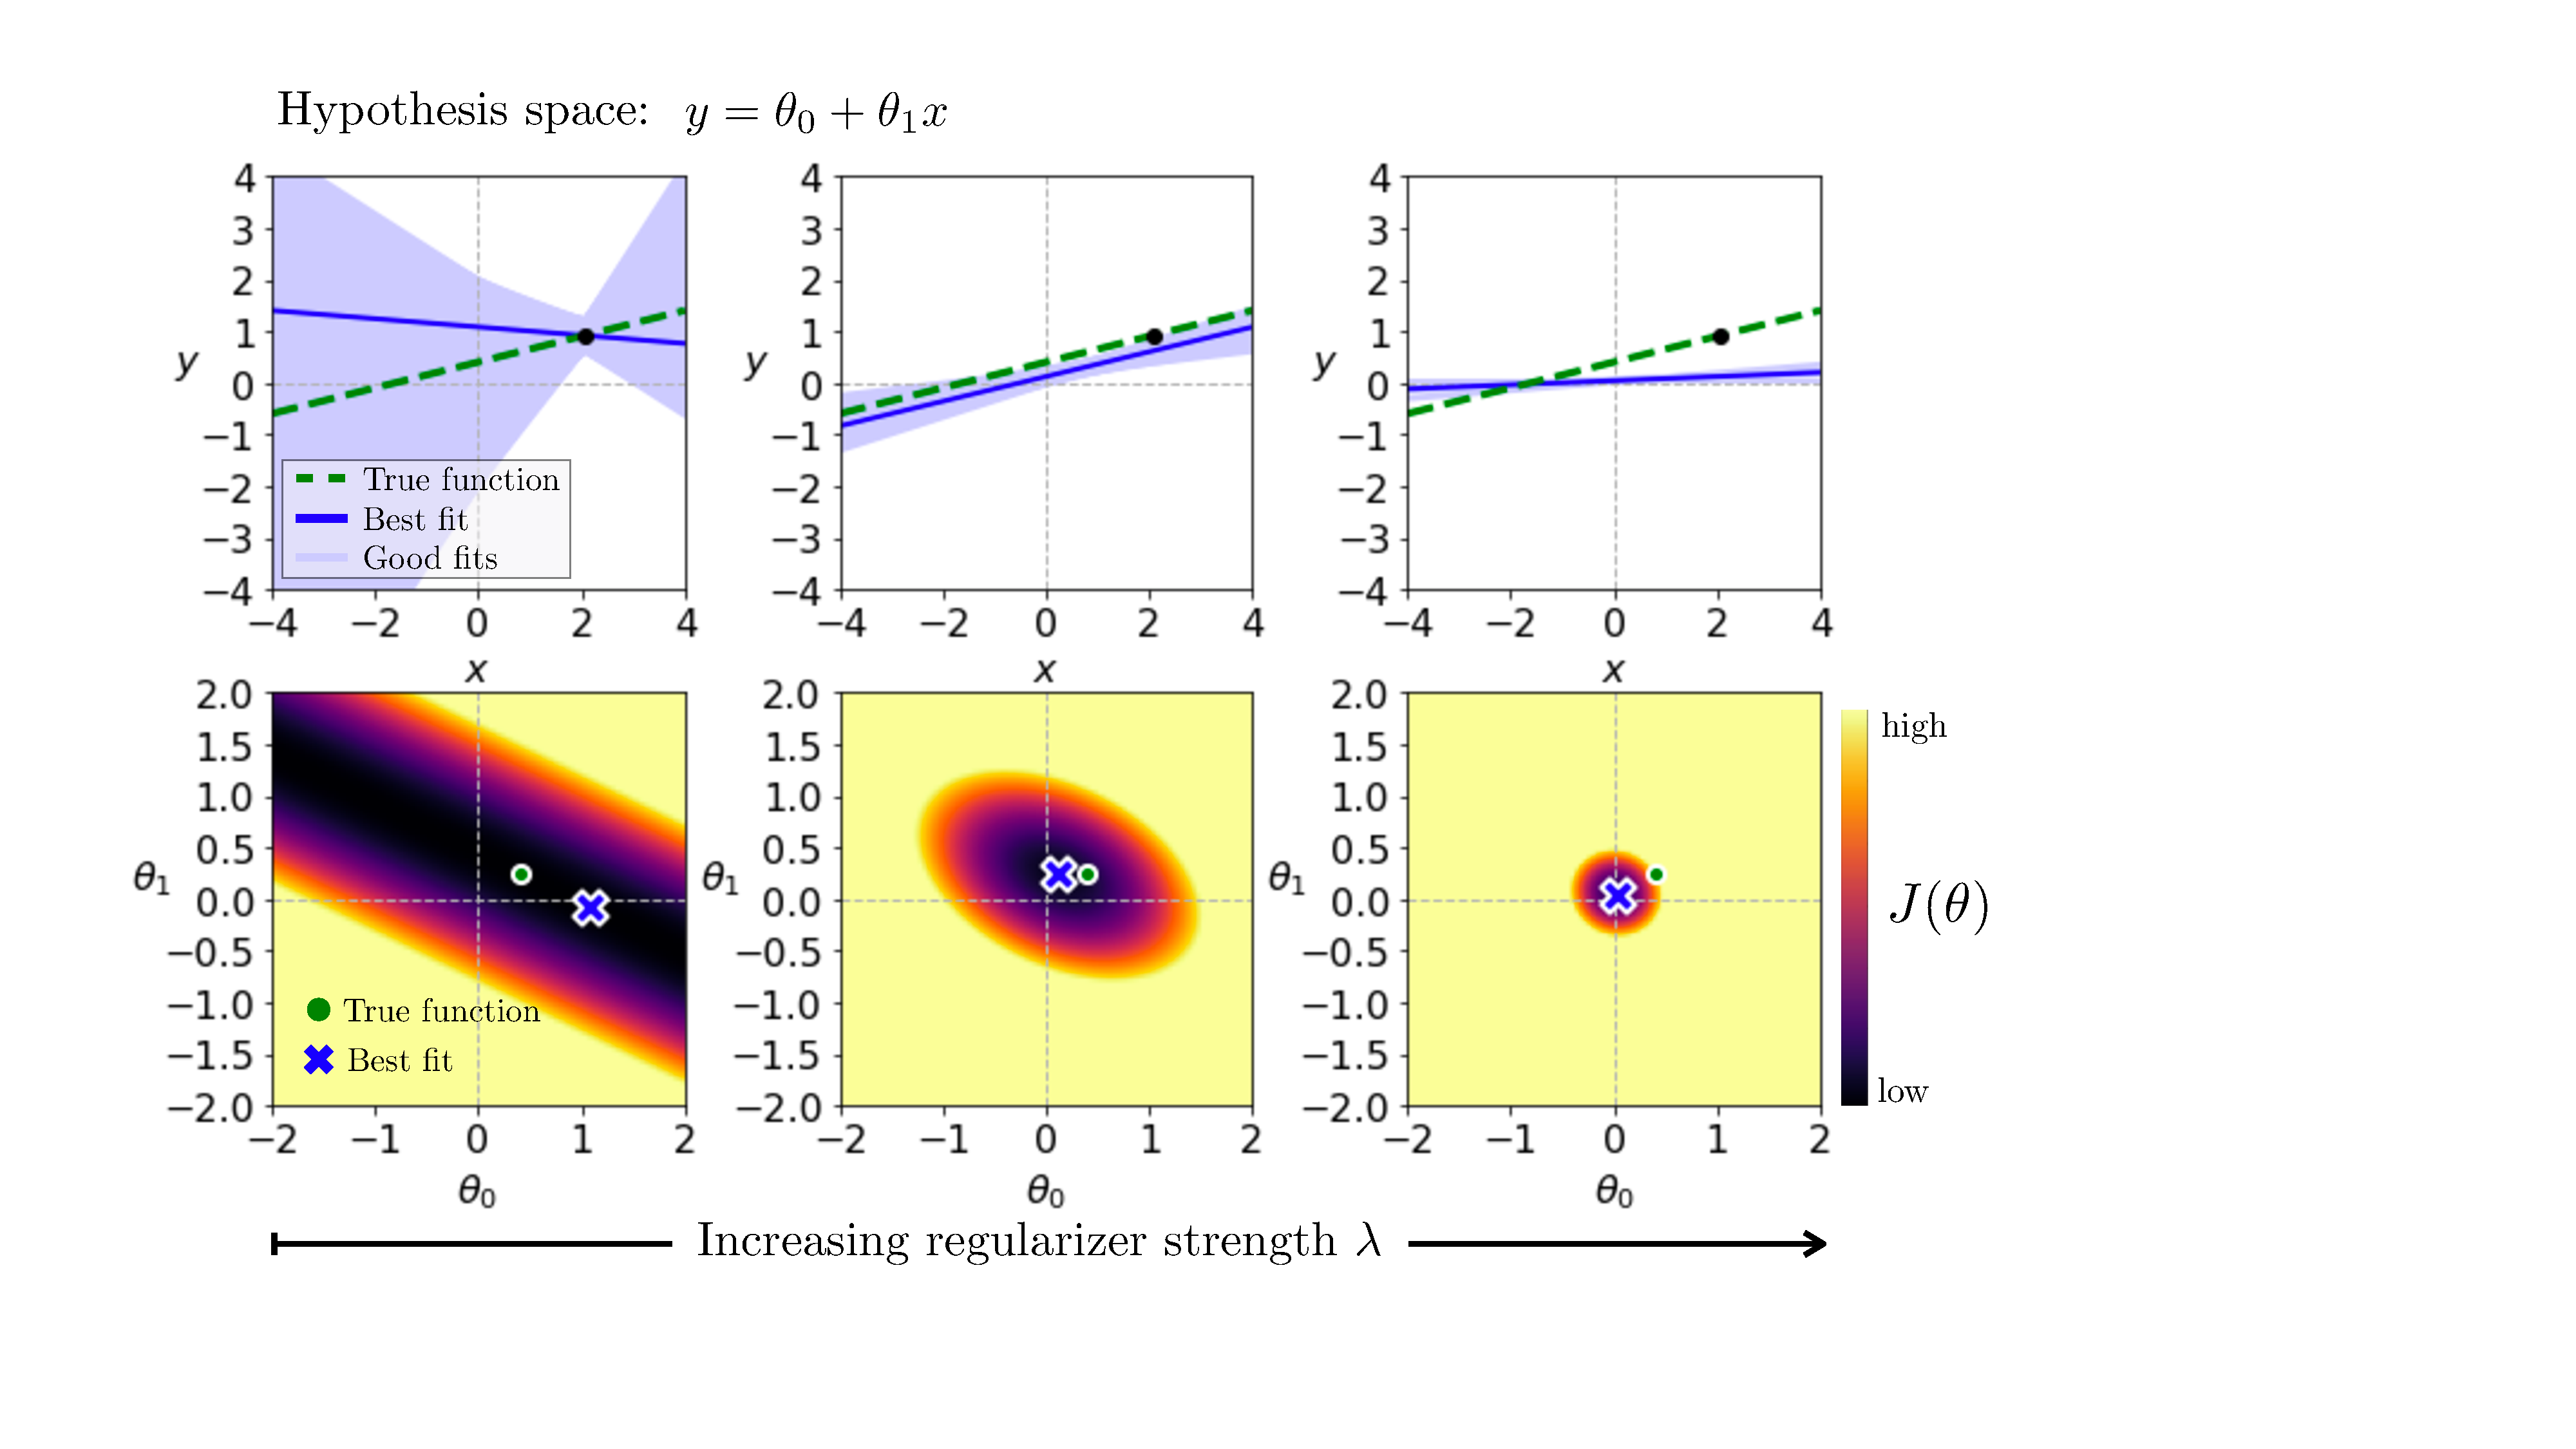
\includegraphics[width=1.0\linewidth]{./figures/problem_of_generalization/more_regularizer_more_constraints.pdf}
    }
    \caption{More regularization, more (soft) constraints.}
    \label{fig:problem_of_generalization:more_regularizer_more_constraints}
\end{figure}

In this example, the true solution lies near the origin, so adding some regularization gets us closer to the truth. But using too strong a $\lambda$ overregularizers; the true solution is not \textit{exactly} $\theta=0$. The middle column is the Goldilocks solution, where the strength of the regularizer is just right.

You can take away a few lessons from this example:
\begin{enumerate}
    \item Priors help only when they are good guesses as to the truth.
    \item Overreliance on the prior means ignoring the data, and this is generally a bad thing.
    \item For any given prior, there is a sweet spot where the strength is optimal. Sometimes this ideal strength can be derived from modeling assumptions and other times you may need to tune it as a hyperparameter.
\end{enumerate}

\subsection{Experiment 3: Effect of the Hypothesis Space}

Now we turn to the last of our tools: the hypothesis space itself. For this experiment, we will use the same objective as in \eqn{\ref{eqn:problem_of_generalization:error_fn_1}} and we will consider the following three hypothesis spaces:
\begin{align}
    f_{\theta}(x) &= \theta_0 x + \theta_1 x^2 &\triangleleft \quad\texttt{quadratic}\\
    f_{\theta}(x) &= \theta_0 x &\triangleleft \quad\texttt{linear}\\
    f_{\theta}(x) &= 0 &\triangleleft \quad\texttt{constant}
\end{align}
Our experiment on these three spaces is shown in \fig{\ref{fig:problem_of_generalization:fewer_hypotheses_more_constraints}}. We show the hypothesis spaces in order of decreasing size moving to the right.

\begin{figure}[t]
    \centerline{
    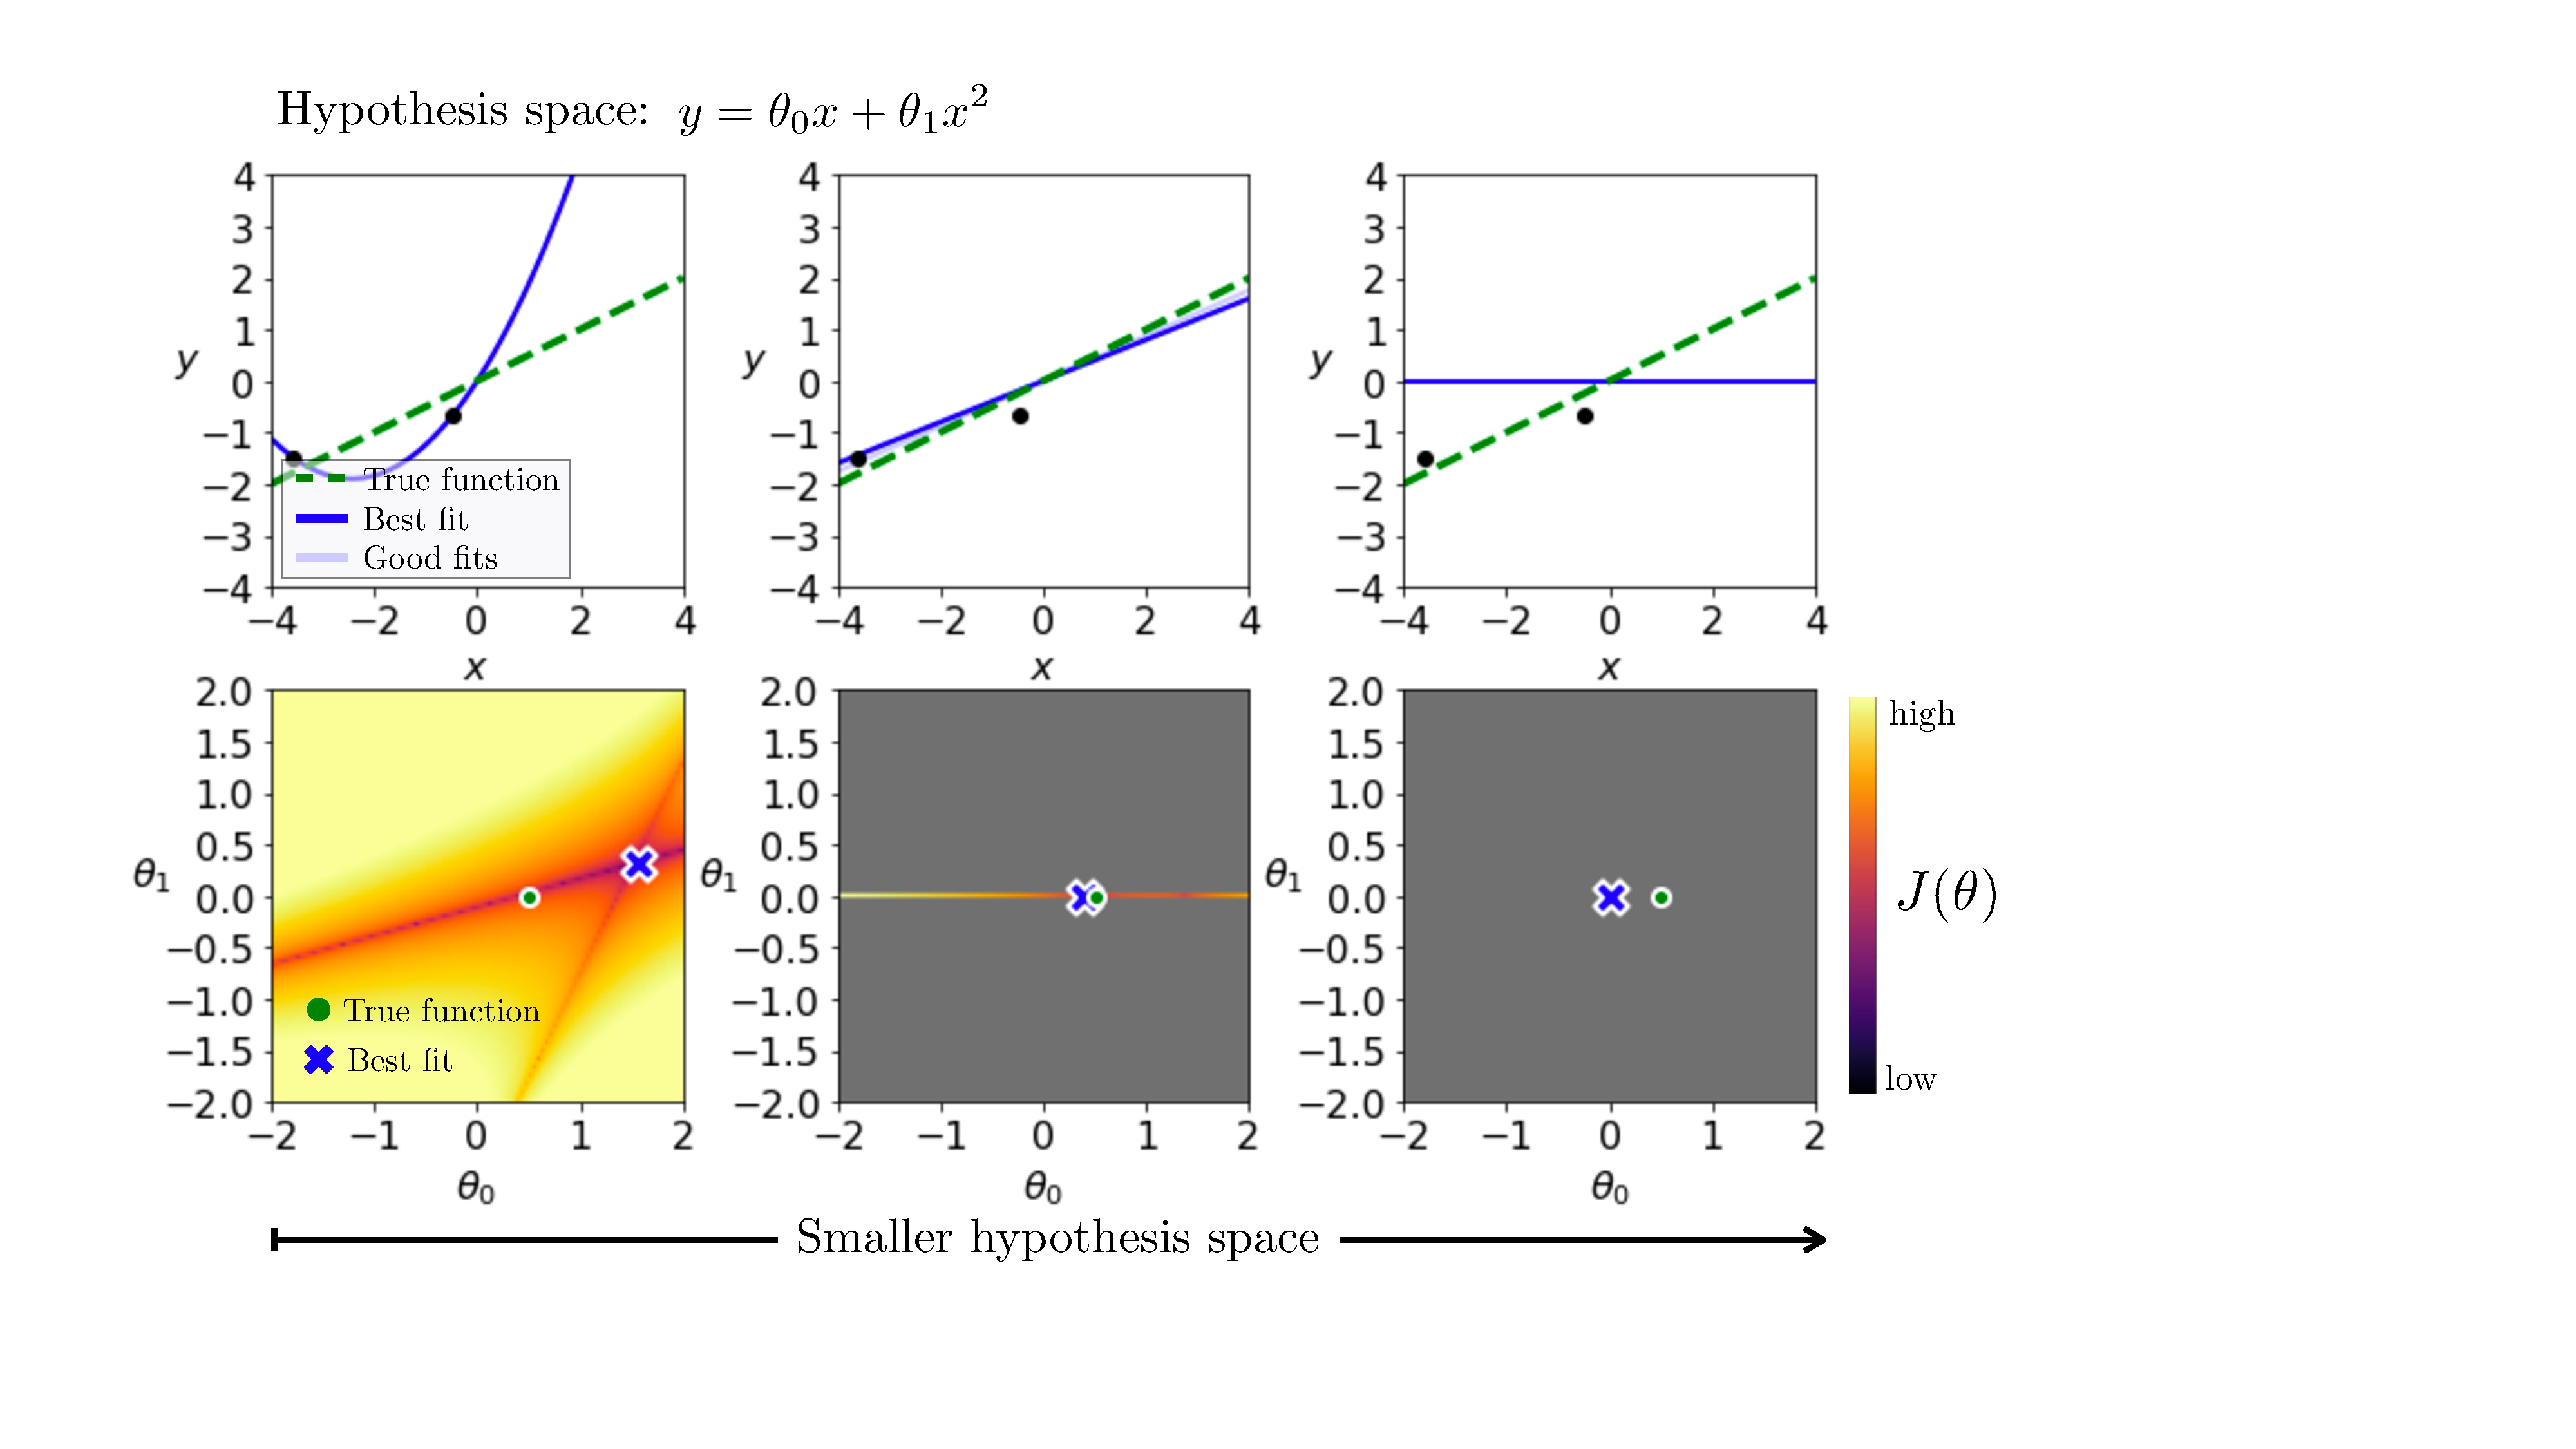
\includegraphics[width=1.0\linewidth]{./figures/problem_of_generalization/fewer_hypotheses_more_constraints.pdf}
    }
    \caption{Fewer hypotheses, more (hard) constraints.}
    \label{fig:problem_of_generalization:fewer_hypotheses_more_constraints}
\end{figure}

The true function is linear, and because of that both the \texttt{quadratic} and \texttt{linear} hypothesis spaces contain the true solution. However, the linear hypothesis space is \textit{much} smaller than the quadratic space. For the linear hypothesis space, searching for the solution (i.e., learning) only considers the slice of parameter space where $\theta_1=0$; all the gray region in \fig{\ref{fig:problem_of_generalization:fewer_hypotheses_more_constraints}} can be ignored. Using a smaller hypothesis space can potentially accelerate our search. %This leads us to a general principle:
%\begin{center}
%    \textit{A smaller hypothesis space can accelerate the search for truth.}
%\end{center}
%\marginnote{Remember, the hypothesis space and parameterization are \textit{not} the same thing (see \chap{\ref{chapter:intro_to_learning}}, \sect{\ref{sec:intro_to_learning:key_ingredients}}). \textit{Overparameterizating} a small hypothesis space can make learning faster.}[-0.4cm]

However, clearly you can go too far, as is demonstrated by the \texttt{constant} hypothesis space (far right column). This hypothesis space only contains one function, namely $f_{\theta}(x) = 0$. Search is trivial, but the truth is not in this space.

%One important thing to note is that the hypothesis space is not the same as the parameterization. The same hypothesis space can be parameterized in many ways. For example, a linear function $\mathbb{R} \rightarrow \mathbb{R}$ can be parameterized either as $f_{\theta}(x) = \theta_0 x$ or as $f_{\theta}(x) = \theta_1 \theta_0 x$, or as $f_{\theta}(x) = (\theta_1 + \theta_0) x$ or infinite other possiblities, as long as the parameters all end up describing a linear function of $x$. All these parameterizations span the same hypothesis space: linear relationships between $x$ and $y$. You might be tempted to think that fewer parameters is better, since a smaller hypothesis space is generally better (as long as it contains the truth). But this is not always the case. \textit{Overparameterized} models, which have more parameters than the minimum necessary to describe the hypothesis space, sometimes confer benefits in terms of implicit regularization and optimization speed~\cite{XX}. The virtues of overparameterization are being actively studied in the context of deep neural nets (which are generally highly overparameterized)~\cite{XX}.

\subsection{Summary of the Experiments}

These three experiments demonstrate that data, priors, and hypotheses can all constrain our search in similar ways. All three rule out some parts of the full space of mappings and help us focus on others. 

This leads us to another general principle:
\begin{center}
    \textit{What can be achieved with any one of our tools can also be achieved with any other.\footnote{However, note that the hypothesis space places \textit{hard} constraints on our search; we cannot violate them. Data and priors apply \textit{soft} constraints; we can violate them but we will pay a penalty.}}
\end{center}
%\marginnote{* However, note that the hypothesis space places \textit{hard} constraints on our search; we cannot violate them. Data and priors apply \textit{soft} constraints; we can violate them but we will pay a penalty.}
If you don't have much data, you can use strong priors and structural constraints instead. If you don't have much domain knowledge, you can collect lots of data instead. This principle was nicely articulated by Ilya Sutskever when he wrote that ``methods ... are extra training data in disguise''~\cite{dataindisguise}. %And we can equally well say: training data is extra methods in disguise.


\section{Concluding Remarks}
The goal of learning is to extract lessons from past data to help on future problem solving. Unless the future is \textit{identical} to the past, this is a problem that requires generalization. One goal of learning algorithms is to make systems that generalize ever better, meaning they continue to work even when the test data is very different than the training data. Currently, however, the systems that generalize in the strongest sense—that work \textit{for all} possible test data—are generally not learned but designed according to other principles. In this way, many classical algorithms still have advantages over the latest learned systems. But this gap is rapidly closing! % PHILLIP
% 
\chapter{Neural Networks}\label{chapter:neural_nets}
%\textit{Draft chapter from Torralba, Isola, Freeman}

\section{Introduction}
Neural networks are functions loosely modeled on the brain. In the brain, we have billions of neurons that connect to one another. Each neuron can be thought of as a node in a graph, and the edges are the connections from one neuron to the next (\fig{\ref{fig:neural_nets:fig1_net}}). The edges are directed; electrical signals propagate in just one direction along the wires in the brain.

\begin{figure}[h]
\centerline{
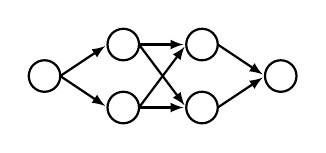
\begin{tikzpicture}%[>=spaced latex]
\draw [thick] (0,0) circle [radius=0.2];
\draw [thick] [nn_edge] (0.2,0) -- (0.8,-0.4);
\draw [thick] [nn_edge] (0.2,0) -- (0.8,0.4);
\draw [thick] (1,-0.4) circle [radius=0.2];
\draw [thick] (1,0.4) circle [radius=0.2];
\draw [thick] [nn_edge] (1.2,-0.4) -- (1.8,-0.4);
\draw [thick] [nn_edge] (1.2,0.4) -- (1.8,0.4);
\draw [thick] [nn_edge] (1.2,-0.4) -- (1.8,0.4);
\draw [thick] [nn_edge] (1.2,0.4) -- (1.8,-0.4);
\draw [thick] (2,-0.4) circle [radius=0.2];
\draw [thick] (2,0.4) circle [radius=0.2];
\draw [thick] [nn_edge] (2.2,-0.4) -- (2.8,0);
\draw [thick] [nn_edge] (2.2,0.4) -- (2.8,0);
\draw [thick] (3.0,0) circle [radius=0.2];
\end{tikzpicture}
}
\caption{A neural network can be drawn as a directed graph.}
\label{fig:neural_nets:fig1_net}
\end{figure}


Outgoing edges are called axons and incoming edges are called dendrites. A neuron fires, sending a pulse down its axon, when the incoming pulses, from the dendrites, exceed a threshold. 

\section{The Perceptron: A Simple Model of a Single Neuron}
Let's consider a neuron, shaded in gray, that has four inputs and one output (\fig{\ref{fig:neural_nets:perceptron_fig2}}).
\begin{figure}[h]
\centerline{
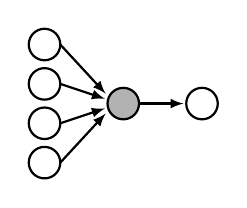
\begin{tikzpicture}[>=spaced latex]
\draw [thick] (0,-0.75) circle [radius=0.2];
\draw [thick] (0,-0.25) circle [radius=0.2];
\draw [thick] (0,0.25) circle [radius=0.2];
\draw [thick] (0,0.75) circle [radius=0.2];
\draw [thick] [nn_edge] (0.2,-0.75) -- (0.8,-0.1);
\draw [thick] [nn_edge] (0.2,-0.25) -- (0.8,-0.05);
\draw [thick] [nn_edge] (0.2,0.25) -- (0.8,0.05);
\draw [thick] [nn_edge] (0.2,0.75) -- (0.8,0.1);
\draw [thick, fill=gray_neuron] (1,0) circle [radius=0.2];
\draw [thick] [nn_edge] (1.2,0) -- (1.8,0);
\draw [thick] (2.0,0) circle [radius=0.2];
\end{tikzpicture}
}
\caption{Perceptron.}
\label{fig:neural_nets:perceptron_fig2}
\end{figure}

A simple model for this neuron is the \index{Perceptron}{\bf perceptron}. A perceptron is a neuron with $n$ inputs $\{x_i\}_{i=1}^n$ and one output $y$, that maps inputs to outputs according to the following equations:
\begin{align}
    z = f(\mathbf{x}) &= \sum_{i=1}^n w_i x_i + b = \mathbf{w}^\transpose\mathbf{x} + b &\triangleleft \quad \text{linear layer}\\
    g(z) &= \begin{cases}
    1, &\text{if} \quad z > 0\\
    0,              & \text{otherwise}
\end{cases} &\triangleleft \quad \text{activation function}\label{eqn:neural_nets:perceptron_activation}\\
    y &= g(f(\mathbf{x})) &\triangleleft \quad \text{perceptron}
\end{align}

In words, we take a weighted sum of the inputs and, if that sum exceeds a threshold (here 0), the neuron fires (outputs a 1). The function $f$ is called a \index{Linear layer}{\bf linear layer} because it computes a linear function of the inputs, $\mathbf{w}^\transpose\mathbf{x}$, plus a \index{Bias}\textbf{bias}, b. The function $g$ is called the \index{Activation function}{\bf activation function} because it decides whether the neuron activates (fires).\marginnote{Mathematically, $f$ is an affine function, but by convention we call it a ``linear layer.'' One way to think of it is $f$ is a linear function of $\begin{bmatrix}\mathbf{x}\\ 1\end{bmatrix}$.}[-0.8cm]

\subsection{The Perceptron as a Classifier}
People got excited about perceptrons in the late 1950s because it was shown that they can learn to classify data~\cite{rosenblatt1958perceptron}. Let's see how that works. We will consider a perceptron with two inputs, $x_1$ and $x_2$, and one output, $y$. Let the incoming connection weights be $w_1 = 2$, $w_2 = 1$, and $b=0$. The values of $z$ and $y$, as a function of $x_1$ and $x_2$, are shown in \fig{\ref{fig:neural_nets:perceptron_as_classifier}}.

\begin{figure}[h]
\centerline{

\noindent\hspace{0.05\linewidth}
\begin{minipage}{.25\linewidth}

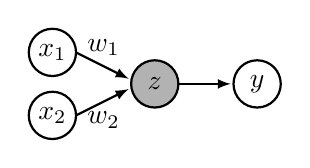
\begin{tikzpicture}[>=spaced latex]
\draw [thick] (0,-0.4) circle [radius=0.3] node {$x_2$};
\draw [thick] (0,0.4) circle [radius=0.3] node {$x_1$};
\draw [thick] [nn_edge] (0.3,-0.4) -- (1.0,-0.05) node[midway,below] {$w_2$};
\draw [thick] [nn_edge] (0.3,0.4) -- (1.0,0.05) node[midway,above] {$w_1$};
\draw [thick, fill=gray_neuron] (1.3,0) circle [radius=0.3] node {$z$};
\draw [thick] [nn_edge] (1.6,0) -- (2.3,0);
\draw [thick] (2.6,0) circle [radius=0.3] node {$y$};
\end{tikzpicture}

\end{minipage}
\begin{minipage}{.68\linewidth}

\begin{tikzpicture}
\begin{axis}[name=plot1, view={0}{90}, xmin=-1, xmax=1, ymin=-1, ymax=1, 
width=0.5\linewidth, xlabel=$x_1$, ylabel=$x_2$, 
title=$z$,
axis equal image,
x label style={at={(axis description cs:0.5,-0.17)}},
y label style={at={(axis description cs:-0.17,0.5)}},
]
	\addplot3[surf, shader=interp, domain=-1:1] {2*x+y};
	\end{axis}
%\end{tikzpicture}
%\end{minipage}
%\begin{minipage}{.30\linewidth}
%\begin{tikzpicture}
\begin{axis}[name=plot2, at=(plot1.right of south east), xshift=30, view={0}{90}, xmin=-1, xmax=1, ymin=-1, ymax=1, 
width=0.5\linewidth, xlabel=$x_1$, ylabel=$x_2$,
title=$y$,
colorbar,
colorbar style={
        ytick={-3.0,-2.0,-1.0,0,1.0,2.0,3.0},
        yticklabel style={
            align=right
        },
        width=5.0
    },
axis equal image,
x label style={at={(axis description cs:0.5,-0.17)}},
y label style={at={(axis description cs:-0.17,0.5)}},
%ymajorticks=false
]
    \addplot3[surf, shader=interp, domain=-1:1] {2*x+y};
	%\addplot[fill] {-2*x} -- cycle;
	\addplot[fill, index of colormap={5 of viridis}, color=.] coordinates 
		{(-1,-1) (0.5,-1) (-0.5,1) (-1,1)} --cycle;
	\addplot[fill, index of colormap={10 of viridis}, color=.] coordinates 
		{(0.5,-1) (1,-1) (1,1) (-0.5,1)} --cycle;
	\end{axis}
\end{tikzpicture}

\end{minipage}
}
\caption{Value of hidden unit ($z$) and output unit ($y$) in a perceptron, as a function of the input data.}
\label{fig:neural_nets:perceptron_as_classifier}
\end{figure}

Notice that $y$ takes on values 0 or 1, so you can think of this as a classifier that assigns a class label of 1 to the upper-right half of the plotted region.

\subsection{Learning with a Perceptron}
So a perceptron acts like a classifier, but how can we use it to learn? The idea is that given data, $\{\mathbf{x}^{(i)}, y^{(i)}\}_{i=1}^N$, we will adjust the weights $\mathbf{w}$ and the bias $b$, in order to minimize a classification loss, $\mathcal{L}$, that scores number of misclassifications:
\begin{align}
    \mathbf{w}^*, b^* = \argmin_{\mathbf{w}, b} \frac{1}{N}\sum_{i=1}^N \mathcal{L}(\mathbf{w}^\transpose\mathbf{x}^{(i)} + b, y^{(i)})\label{eqn:neural_nets:perceptron_learning_problem}
\end{align}
In \fig{\ref{fig:neural_nets:fitting_a_perceptron}}, this optimization process corresponds to shifting and rotating the \textbf{decision boundary}, until you find a line that separates data labeled as $y = 0$ from data labeled as $y = 1$.
\begin{figure}[h]
%\centerline{
%\noindent\hspace{0.05\linewidth}
\begin{minipage}{0.32\linewidth}
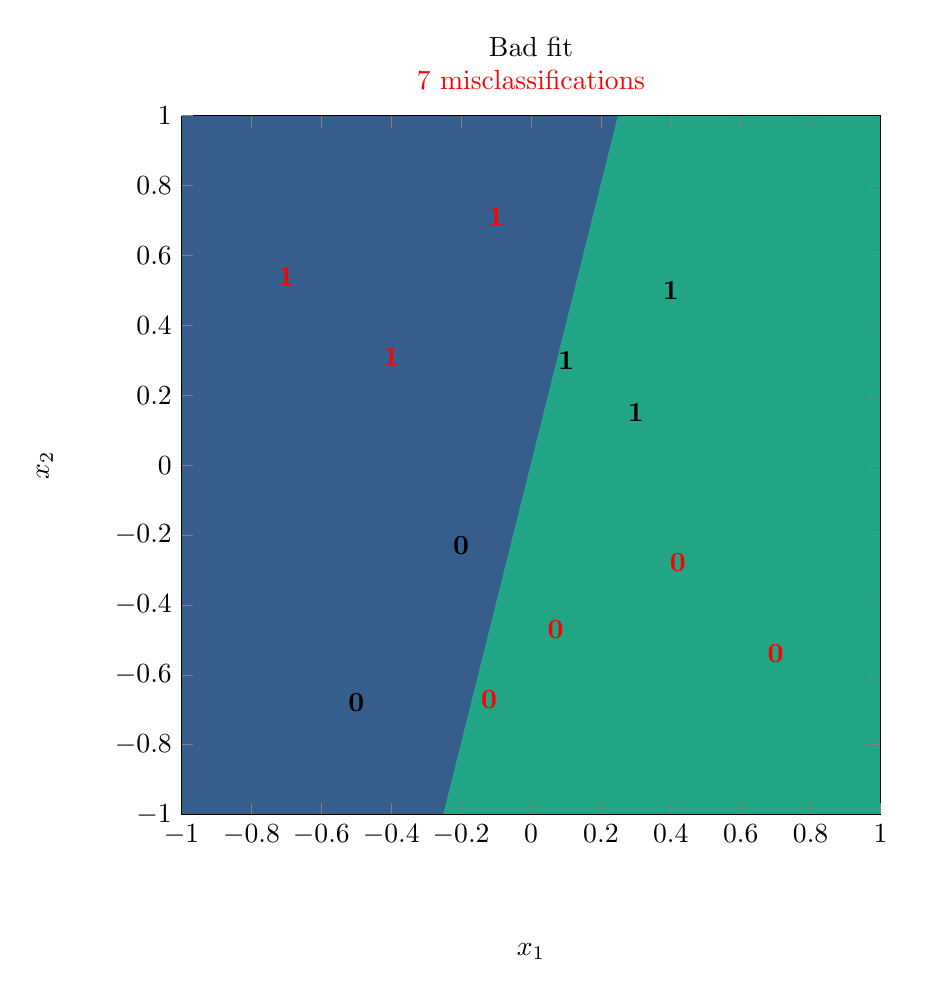
\begin{tikzpicture}
\begin{axis}[view={0}{90}, xmin=-1, xmax=1, ymin=-1, ymax=1, 
width=1.0\linewidth, xlabel=$x_1$, ylabel=$x_2$,
align=center,
title={Bad fit\\\color{red} 7 misclassifications},
axis equal image,
x label style={at={(axis description cs:0.5,-0.17)}},
y label style={at={(axis description cs:-0.17,0.5)}},
scatter/classes={%
    pos_correct={mark=text, text mark={\bf 1}},%
    pos_incorrect={mark=text, text mark={\bf \color{red} 1}},%
    neg_correct={mark=text, text mark={\bf 0}},%
    neg_incorrect={mark=text, text mark={\bf \color{red} 0}}}]
%
\addplot3[surf, shader=interp, domain=-1:1] {2*x+y};
	%\addplot[fill] {-2*x} -- cycle;
	\addplot[fill, index of colormap={5 of viridis}, color=.] coordinates 
		{(-1,-1) (-1,1) (0.25,1) (-0.25,-1)} --cycle;
	\addplot[fill, index of colormap={10 of viridis}, color=.] coordinates 
		{(0.25,1) (1,1) (1,-1) (-0.25,-1)} --cycle;

\addplot[scatter,only marks,%
    scatter src=explicit symbolic]%
table[meta=label] {
x y label
0.1 0.3 pos_correct
0.3 0.15 pos_correct
0.4 0.5 pos_correct
-0.1 0.71 pos_incorrect
-0.4 0.31 pos_incorrect
-0.7 0.54 pos_incorrect
%
-0.5 -0.68 neg_correct
-0.2 -0.23 neg_correct
-0.12 -0.67 neg_incorrect
0.07 -0.47 neg_incorrect
0.42 -0.28 neg_incorrect
0.7 -0.54 neg_incorrect
    };
\end{axis}
\end{tikzpicture}
\end{minipage}
%
%
\begin{minipage}{0.32\linewidth}
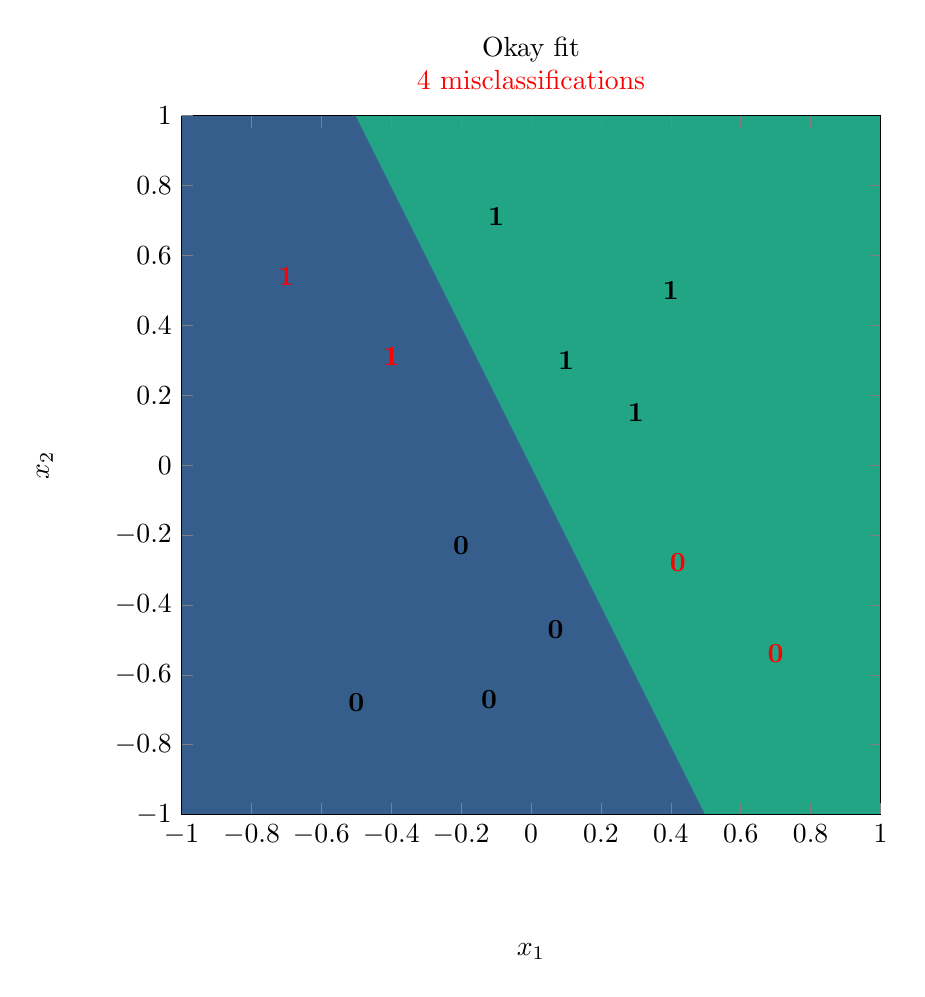
\begin{tikzpicture}
\begin{axis}[view={0}{90}, xmin=-1, xmax=1, ymin=-1, ymax=1, 
width=1.0\linewidth, xlabel=$x_1$, ylabel=$x_2$,
align=center,
title={Okay fit\\\color{red} 4 misclassifications},
axis equal image,
x label style={at={(axis description cs:0.5,-0.17)}},
y label style={at={(axis description cs:-0.17,0.5)}},
scatter/classes={%
    pos_correct={mark=text, text mark={\bf 1}},%
    pos_incorrect={mark=text, text mark={\bf \color{red} 1}},%
    neg_correct={mark=text, text mark={\bf 0}},%
    neg_incorrect={mark=text, text mark={\bf \color{red} 0}}}]
%
\addplot3[surf, shader=interp, domain=-1:1] {2*x+y};
	%\addplot[fill] {-2*x} -- cycle;
	\addplot[fill, index of colormap={5 of viridis}, color=.] coordinates 
		{(-1,-1) (0.5,-1) (-0.5,1) (-1,1)} --cycle;
	\addplot[fill, index of colormap={10 of viridis}, color=.] coordinates 
		{(0.5,-1) (1,-1) (1,1) (-0.5,1)} --cycle;
%
\addplot[scatter,only marks,%
    scatter src=explicit symbolic]%
table[meta=label] {
x y label
0.1 0.3 pos_correct
0.3 0.15 pos_correct
0.4 0.5 pos_correct
-0.1 0.71 pos_correct
-0.4 0.31 pos_incorrect
-0.7 0.54 pos_incorrect
%
-0.12 -0.67 neg_correct
-0.2 -0.23 neg_correct
-0.5 -0.68 neg_correct
0.07 -0.47 neg_correct
0.42 -0.28 neg_incorrect
0.7 -0.54 neg_incorrect
    };
\end{axis}
\end{tikzpicture}
\end{minipage}
%
%
\begin{minipage}{0.32\linewidth}
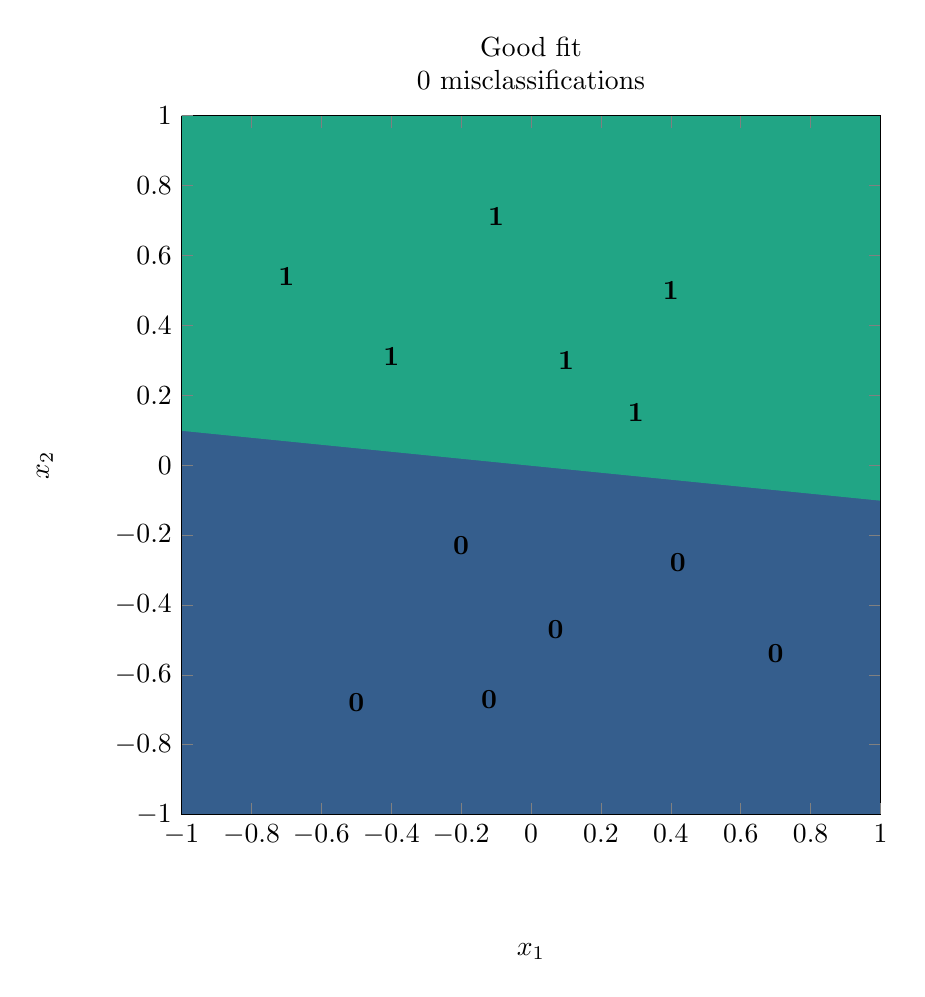
\begin{tikzpicture}
\begin{axis}[view={0}{90}, xmin=-1, xmax=1, ymin=-1, ymax=1, 
width=1.0\linewidth, xlabel=$x_1$, ylabel=$x_2$,
align=center,
title={Good fit\\0 misclassifications},
axis equal image,
x label style={at={(axis description cs:0.5,-0.17)}},
y label style={at={(axis description cs:-0.17,0.5)}},
scatter/classes={%
    pos_correct={mark=text, text mark={\bf 1}},%
    pos_incorrect={mark=text, text mark={\bf \color{red} 1}},%
    neg_correct={mark=text, text mark={\bf 0}},%
    neg_incorrect={mark=text, text mark={\bf \color{red} 0}}}]
%
\addplot3[surf, shader=interp, domain=-1:1] {2*x+y};
	%\addplot[fill] {-2*x} -- cycle;
	\addplot[fill, index of colormap={5 of viridis}, color=.] coordinates 
		{(-1,-1) (1,-1) (1,-0.1) (-1,0.1)} --cycle;
	\addplot[fill, index of colormap={10 of viridis}, color=.] coordinates 
		{(-1,0.1) (-1,1) (1,1) (1,-0.1)} --cycle;
%
\addplot[scatter,only marks,%
    scatter src=explicit symbolic]%
table[meta=label] {
x y label
0.1 0.3 pos_correct
0.3 0.15 pos_correct
0.4 0.5 pos_correct
-0.1 0.71 pos_correct
-0.4 0.31 pos_correct
-0.7 0.54 pos_correct
%
-0.12 -0.67 neg_correct
-0.2 -0.23 neg_correct
-0.5 -0.68 neg_correct
0.07 -0.47 neg_correct
0.42 -0.28 neg_correct
0.7 -0.54 neg_correct
    };
\end{axis}
\end{tikzpicture}
\end{minipage}
\caption{Different possible decision surfaces of a perceptron.}
\label{fig:neural_nets:fitting_a_perceptron}
\end{figure}

You might be wondering, what's the exact optimization algorithm that will find the best line that separates the classes? The original perceptron paper proposed one particular algorithm, the ``perceptron learning algorithm.'' This was an optimizer tailored to the specific structure of the perceptron. Older papers on neural nets are full of specific learning rules for specific architectures: the delta rule, the Rescorla-Wagner model, and so forth~\cite{rescorla1972theory}. Nowadays we rarely use these special-purpose algorithms. Instead, we use \textit{general-purpose} optimizers like gradient descent (for differentiable objectives) or zeroth-order methods (for nondifferentiable objectives). The next chapter will cover the backpropagation algorithm, which is a general-purpose gradient-based optimizer that applies to essentially all neural networks we will see in this book (but, note that for the perceptron objective, because it has a nondifferentiable threshold function, we would instead opt for a zeroth order optimizer).

\section{Multilayer Perceptrons}
Perceptrons can solve linearly separable binary classification problems, but they are otherwise rather limited. For one, they only produce a single output. What if we want multiple outputs? We can achieve this by adding edges that fan out after the perceptron (\fig{\ref{fig:neural_nets:fan_out}}).
%What if we want to output probabilities for $k$ different classes?
%What if we want to output continuous values rather than just zeros and ones? This brings us to the general purpose neuron that is the building block of almost all modern neural nets:
\begin{figure}[h]
\centerline{
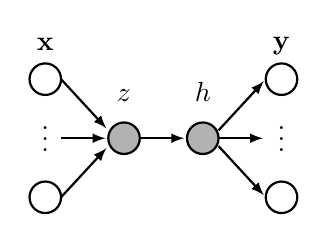
\begin{tikzpicture}[>=spaced latex]
\draw [thick] (0,-0.75) circle [radius=0.2] node[label={$\mathbf{x}$}] at (0,0.85) {};
\draw [thick] (0,0.1) node {$\vdots$};
\draw [thick] (0,0.75) circle [radius=0.2];
\draw [thick] [nn_edge] (0.2,-0.75) -- (0.8,-0.1);
\draw [thick] [nn_edge] (0.2,0.0) -- (0.8,0.0);
\draw [thick] [nn_edge] (0.2,0.75) -- (0.8,0.1);
\draw [thick, fill=gray_neuron] (1,0) circle [radius=0.2]  node[label={$z$}] at (1.0,0.2) {};
\draw [thick] [nn_edge] (1.2,0.0) -- (1.8,0.0);
\draw [thick, fill=gray_neuron] (2.0,0) circle [radius=0.2]  node[label={$h$}] at (2.0,0.2) {};
\draw [thick] [nn_edge] (2.2,-0.1) -- (2.8,-0.75);
\draw [thick] [nn_edge] (2.2,0.0) -- (2.8,0.0);
\draw [thick] [nn_edge] (2.2,0.1) -- (2.8,0.75);
\draw [thick] (3.0,-0.75) circle [radius=0.2] node[label={$\mathbf{y}$}] at (3.0,0.8) {};
\draw [thick] (3.0,0.1)  node {$\vdots$};
\draw [thick] (3.0,0.75) circle [radius=0.2];
\end{tikzpicture}
}
\caption{Multiple outputs fan out from a neuron.}
\label{fig:neural_nets:fan_out}
\end{figure}

This network maps an input {\bf layer} of data $\mathbf{x}$ to a layer of outputs {\bf y}. The neurons in between inputs and outputs are called {\bf hidden units}, shaded in gray. Here, $z$ is a \index{Preactivaton unit}{\bf preactivation} hidden unit and $h$ is a \index{Postactivation unit}{\bf postactivation} hidden unit, that is, $h = g(z)$ where $g(\cdot)$ is an activation function like in \eqn{\ref{eqn:neural_nets:perceptron_activation}}.

More commonly we might have many hidden units in stack, which we call a \index{Hidden layer}{\bf hidden layer} (\fig{\ref{fig:neural_nets:MLP1}}).
%The diagram above has one hidden layer, with a single neuron $h$, called a {\bf hidden unit}
\begin{figure}[h]
\centerline{
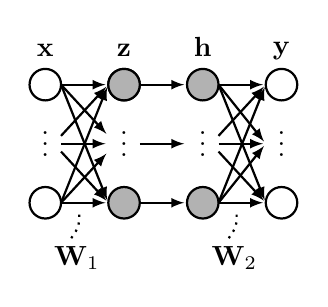
\begin{tikzpicture}[>=spaced latex]
\draw [thick] (0,-0.75) circle [radius=0.2] node[label={$\mathbf{x}$}] at (0,0.85) {};
\draw [thick] (0,0.1) node {$\vdots$};
\draw [thick] (0,0.75) circle [radius=0.2];

\draw [thick,dotted] (0.33,-1.2)  .. controls (0.43,-1.05) .. (0.43,-0.9);
\draw (0.4,-1.45) node {$\mathbf{W}_1$};

\draw [thick] [nn_edge] (0.2,-0.75) -- (0.8,-0.1);
\draw [thick] [nn_edge] (0.2,-0.75) -- (0.8,-0.75);
\draw [thick] [nn_edge] (0.2,-0.75) -- (0.8,0.75);
\draw [thick] [nn_edge] (0.2,-0.1) -- (0.8,-0.75);
\draw [thick] [nn_edge] (0.2,0.0) -- (0.8,0.0);
\draw [thick] [nn_edge] (0.2,0.1) -- (0.8,0.75);
\draw [thick] [nn_edge] (0.2,0.75) -- (0.8,0.75);
\draw [thick] [nn_edge] (0.2,0.75) -- (0.8,-0.75);
\draw [thick] [nn_edge] (0.2,0.75) -- (0.8,0.1);
\draw [thick, fill=gray_neuron] (1,0.75) circle [radius=0.2]  node[label={$\mathbf{z}$}] at (1.0,0.85) {};
\draw [thick] (1,0.1) node {$\vdots$};
\draw [thick, fill=gray_neuron] (1,-0.75) circle [radius=0.2];
\draw [thick] [nn_edge] (1.2,0.75) -- (1.8,0.75);
\draw [thick] [nn_edge] (1.2,0.0) -- (1.8,0.0);
\draw [thick] [nn_edge] (1.2,-0.75) -- (1.8,-0.75);
\draw [thick, fill=gray_neuron] (1,0.75) circle [radius=0.2]  node[label={$\mathbf{h}$}] at (2.0,0.85) {};
\draw [thick, fill=gray_neuron] (2.0,0.75) circle [radius=0.2];
\draw [thick] (2.0,0.1) node {$\vdots$};
\draw [thick, fill=gray_neuron] (2.0,-0.75) circle [radius=0.2];

\draw [thick,dotted] (2.33,-1.2)  .. controls (2.43,-1.05) .. (2.43,-0.9);
\draw (2.4,-1.45) node {$\mathbf{W}_2$};

\draw [thick] [nn_edge] (2.2,-0.75) -- (2.8,-0.75);
\draw [thick] [nn_edge] (2.2,-0.75) -- (2.8,0.75);
\draw [thick] [nn_edge] (2.2,-0.75) -- (2.8,0.0);
\draw [thick] [nn_edge] (2.2,-0.1) -- (2.8,-0.75);
\draw [thick] [nn_edge] (2.2,0.0) -- (2.8,0.0);
\draw [thick] [nn_edge] (2.2,0.1) -- (2.8,0.75);
\draw [thick] [nn_edge] (2.2,0.75) -- (2.8,0.75);
\draw [thick] [nn_edge] (2.2,0.75) -- (2.8,-0.75);
\draw [thick] [nn_edge] (2.2,0.75) -- (2.8,0.0);
\draw [thick] (3.0,-0.75) circle [radius=0.2] node[label={$\mathbf{y}$}] at (3.0,0.8) {};
\draw [thick] (3.0,0.1)  node {$\vdots$};
\draw [thick] (3.0,0.75) circle [radius=0.2];
\end{tikzpicture}
}
\caption{Mutilayer perceptron.}
\label{fig:neural_nets:MLP1}
\end{figure}
\marginnote{How many layers does this net have? Some texts will say two [$\mathbf{W}_1$, $\mathbf{W}_2$], others three [$\mathbf{x}$, $\{\mathbf{z}, \mathbf{h}\}$, $\mathbf{y}$], others four [$\mathbf{x}$, $\mathbf{z}$, $\mathbf{h}$, $\mathbf{y}$]. We must get comfortable with the ambiguity.}[2cm]
% In biology, $h_i$ and $y_i$ are two parts of a single neuron, but often in artificial neural nets we call each node in these diagrams a ``neuron".

Because this network has multiple layers of neurons, and because each neuron in this net acts as a perceptron, we call it a \index{Multilayer perceptron}\textbf{multilayer perceptron} (\textbf{MLP}). The equation for this MLP is:
\begin{align}
    \mathbf{z} &= \mathbf{W}_1\mathbf{x} + \mathbf{b}_1 &\triangleleft \quad \text{linear layer}\\
    \mathbf{h} &= g(\mathbf{z}) &\triangleleft \quad \text{activation function}\\
    \mathbf{y} &= \mathbf{W}_2\mathbf{h} + \mathbf{b}_2 &\triangleleft \quad \text{linear layer}
\end{align}
In general, MLPs can be constructed with any number of layers following this pattern: linear layer, activation function, linear layer, activation function, and so on.

The activation function $g$ could be the threshold function like in \eqn{\ref{eqn:neural_nets:perceptron_activation}}, but more generally it can be any pointwise nonlinearity, that is, $g(\mathbf{h}) = [\tilde{g}(h_1), \ldots, \tilde{g}(h_N)]$ and $\tilde{g}$ is any nonlinear function that maps $\mathbb{R} \rightarrow \mathbb{R}$.

Beyond MLPs, this kind of sequence (linear layer, pointwise nonlinearity, linear layer, pointwise nonlinearity, and so on) is the prototpyical motif in almost all neural networks, including most we will see later in this book.

\section{Activations Versus Parameters}

When working with deep nets it's useful to distinguish \emph{activations} and \emph{parameters}. The activations are the values that the neurons take on, $[\mathbf{x}, \mathbf{z}_1, \mathbf{h}_1, \ldots, \mathbf{z}_{L-1}, \mathbf{h}_{L-1}, \mathbf{y}]$; slightly abusing notation, we use this term for both preactivation function neurons and postactivation function neurons. The activations are the neural representations of the data being processed. Often, we will not worry about distinguishing between inputs, hidden units, and outputs to the net, and simply refer to all data and neural activations in a network, layer by layer, as a sequence $[\mathbf{x}_0, \ldots, \mathbf{x}_L]$, in which case $\mathbf{x}_0$ is the raw input data.

\marginnote{
A multilayer network is a sequence of transformations $f_1, \ldots, f_L$ that produce a series of activations $\mathbf{x}_1, \ldots, \mathbf{x}_L$: 
\\[6pt]
\begin{center}
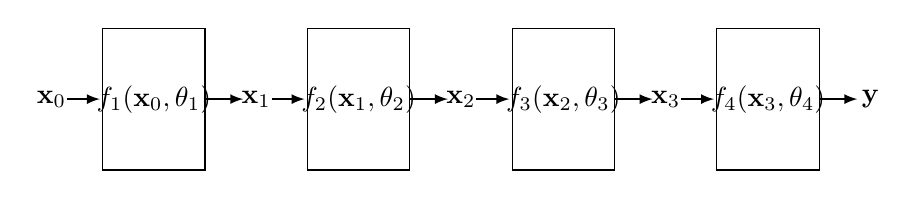
\begin{tikzpicture}
    \def\layerheight{0.8}
    \def\layerwidth{1.3}
    \def\blockheight{1.8}
    \def\blockwidth{1.3}
    % draw f's
    \foreach \x in {0,1,2,3} {
        \pgfmathsetmacro{\index}{int(\x+1)}
        \draw [fill=white] (2*\layerwidth*\x,-0.5*\blockheight) rectangle ++(\blockwidth,\blockheight) node[midway] {$f_{\index}(\mathbf{x}_{\x}, \theta_{\index})$};
    }
    % draw x's
    \foreach \x in {0,1,2,3} {
        \pgfmathsetmacro{\index}{int(\x+1)}
        \draw (2*\layerwidth*\x+0.5*\blockwidth-\layerwidth,0) node {$\mathbf{x}_\x$}; 
    }
    % draw arrows
    %\foreach \x in {0,1,2,3,4,5,6} {
    \foreach \x in {0,2,4,6} {
        %\draw [thick] [nn_edge] (0,\layerheight*\x+\blockheight) -- (0,\layerheight*\x+\layerheight);
        \draw [thick] [nn_edge] (\layerwidth*\x+\blockwidth,0) -- (\layerwidth*\x+\blockwidth+0.4*\layerwidth,0);
        \draw [thick] [nn_edge] (\layerwidth*\x+\blockwidth+0.65*\layerwidth-2*\layerwidth,0) -- (\layerwidth*\x+\blockwidth+\layerwidth-2*\layerwidth,0);
    }
    %\draw [thick] [nn_edge] (0,\layerheight*-1+\blockheight) -- (0,\layerheight*-1+\layerheight);
    \draw (7*\layerwidth+0.5*\blockwidth,0) node {$\mathbf{y}$}; 
\end{tikzpicture}
\end{center}
}[-2.2cm]

Conversely, parameters are the weights and biases of the network. These are the variables being learned. Both activations and parameters are tensors of variables.

Often we think of a layer as a function $\mathbf{x}_{l+1} = f_{l+1}(\mathbf{x}_l)$, but we can also make the parameters explicit and think of each layer as a function:
\begin{align}
    \mathbf{x}_{l+1} = f_{l+1}(\mathbf{x}_{l}, \theta_{l+1})
\end{align}
That is, each layer takes the activations from the previous layer, as well as parameters of the current layer as input, and produces activations of the next layer. Varying either the input activations or the input parameters will affect the output of the layer. From this perspective, anything we can do with parameters, we can do with activations instead, and vice versa, and that is the basis for a lot of applications and tricks. For example, while normally we learn the values of the parameters, we could instead hold the parameters fixed and learn the values of the activations that achieve some objective. In fact, this is what is done in many methods such as network prompting, adversarial attacks, and network visualization, which we will see in more detail in later chapters.
% \subsection{Data vs parameters}

% When working with deep nets it's useful to distinguish \emph{data} and \emph{parameters}. The ``data" are the values that the nodes take on, $[\mathbf{x}, \mathbf{z}_1, \mathbf{h}_1, \ldots, \mathbf{z}_{L-1}, \mathbf{h}_{L-1}, \mathbf{y}]$. It may seem strange at first to call all these variables data, but the idea is that all these values are \textit{representations} of the signal being processed. The inputs $\mathbf{x}$ are a ``raw" representation of the signal whereas later layers of neurons are transformed representations. Often, we will not worry about distinguishing between inputs, hidden units, and outputs, and simply refer to the data in a network, layer by layer, as a sequence $[\mathbf{x}_1, \ldots, \mathbf{x}_L]$.

% Parameters are the weights and biases mentioned above. These are the variables being learned. Both data and parameters are tensors of variables.

% Often we think of a layer as a function $\mathbf{x}_{l+1} = f_{l+1}(\mathbf{x}_l)$, but we can also make the parameters explicit and think of each layer as a function:
% \begin{align}
%     \mathbf{x}_{l+1} = f_{l+1}(\mathbf{x}_{l}, \theta_{l+1})
% \end{align}
% That is, each layer takes the data from the previous layer, as well as parameters of the current layer as input, and produces data of the next layer. Varying either the input data or the input parameters will affect the output of the layer. From this perspective, anything we can do with parameters, we can do with data instead, and vice versa, and that is the basis for a lot of applications and tricks. For example, while normally we learn the values of the parameters, we could instead hold the parameters fixed and learn the values of the data that achieve some objective. In fact this is what is done in applications such as style transfer, adversarial attacks, and network visualization, which we will see in more detail in later chapters.


\subsection{Fast Activations and Slow Parameters}%{\small [Advanced topic]}}
So what's different about activations versus parameters? One way to think about it is that activations are \textit{fast} functions of a data\textit{point}: they are the result of a few layers of processing this datapoint. Parameters are \textit{also} functions of the data (they are learned from data) but they are \textit{slow} functions of data\textit{sets}: the parameters are arrived at via an optimization procedure over a whole dataset. So, both activations and parameters are statistics of the data, that is, information extracted about about the data that organizes or summarizes it. The parameters are a kind of metasummary since they specify a functional transformation that produces activations from data, and activations themselves are a summary of the data. \Fig{\ref{fig:neural_nets:params_vs_activations}} shows how this looks.
\begin{figure}[h]
\centerline{
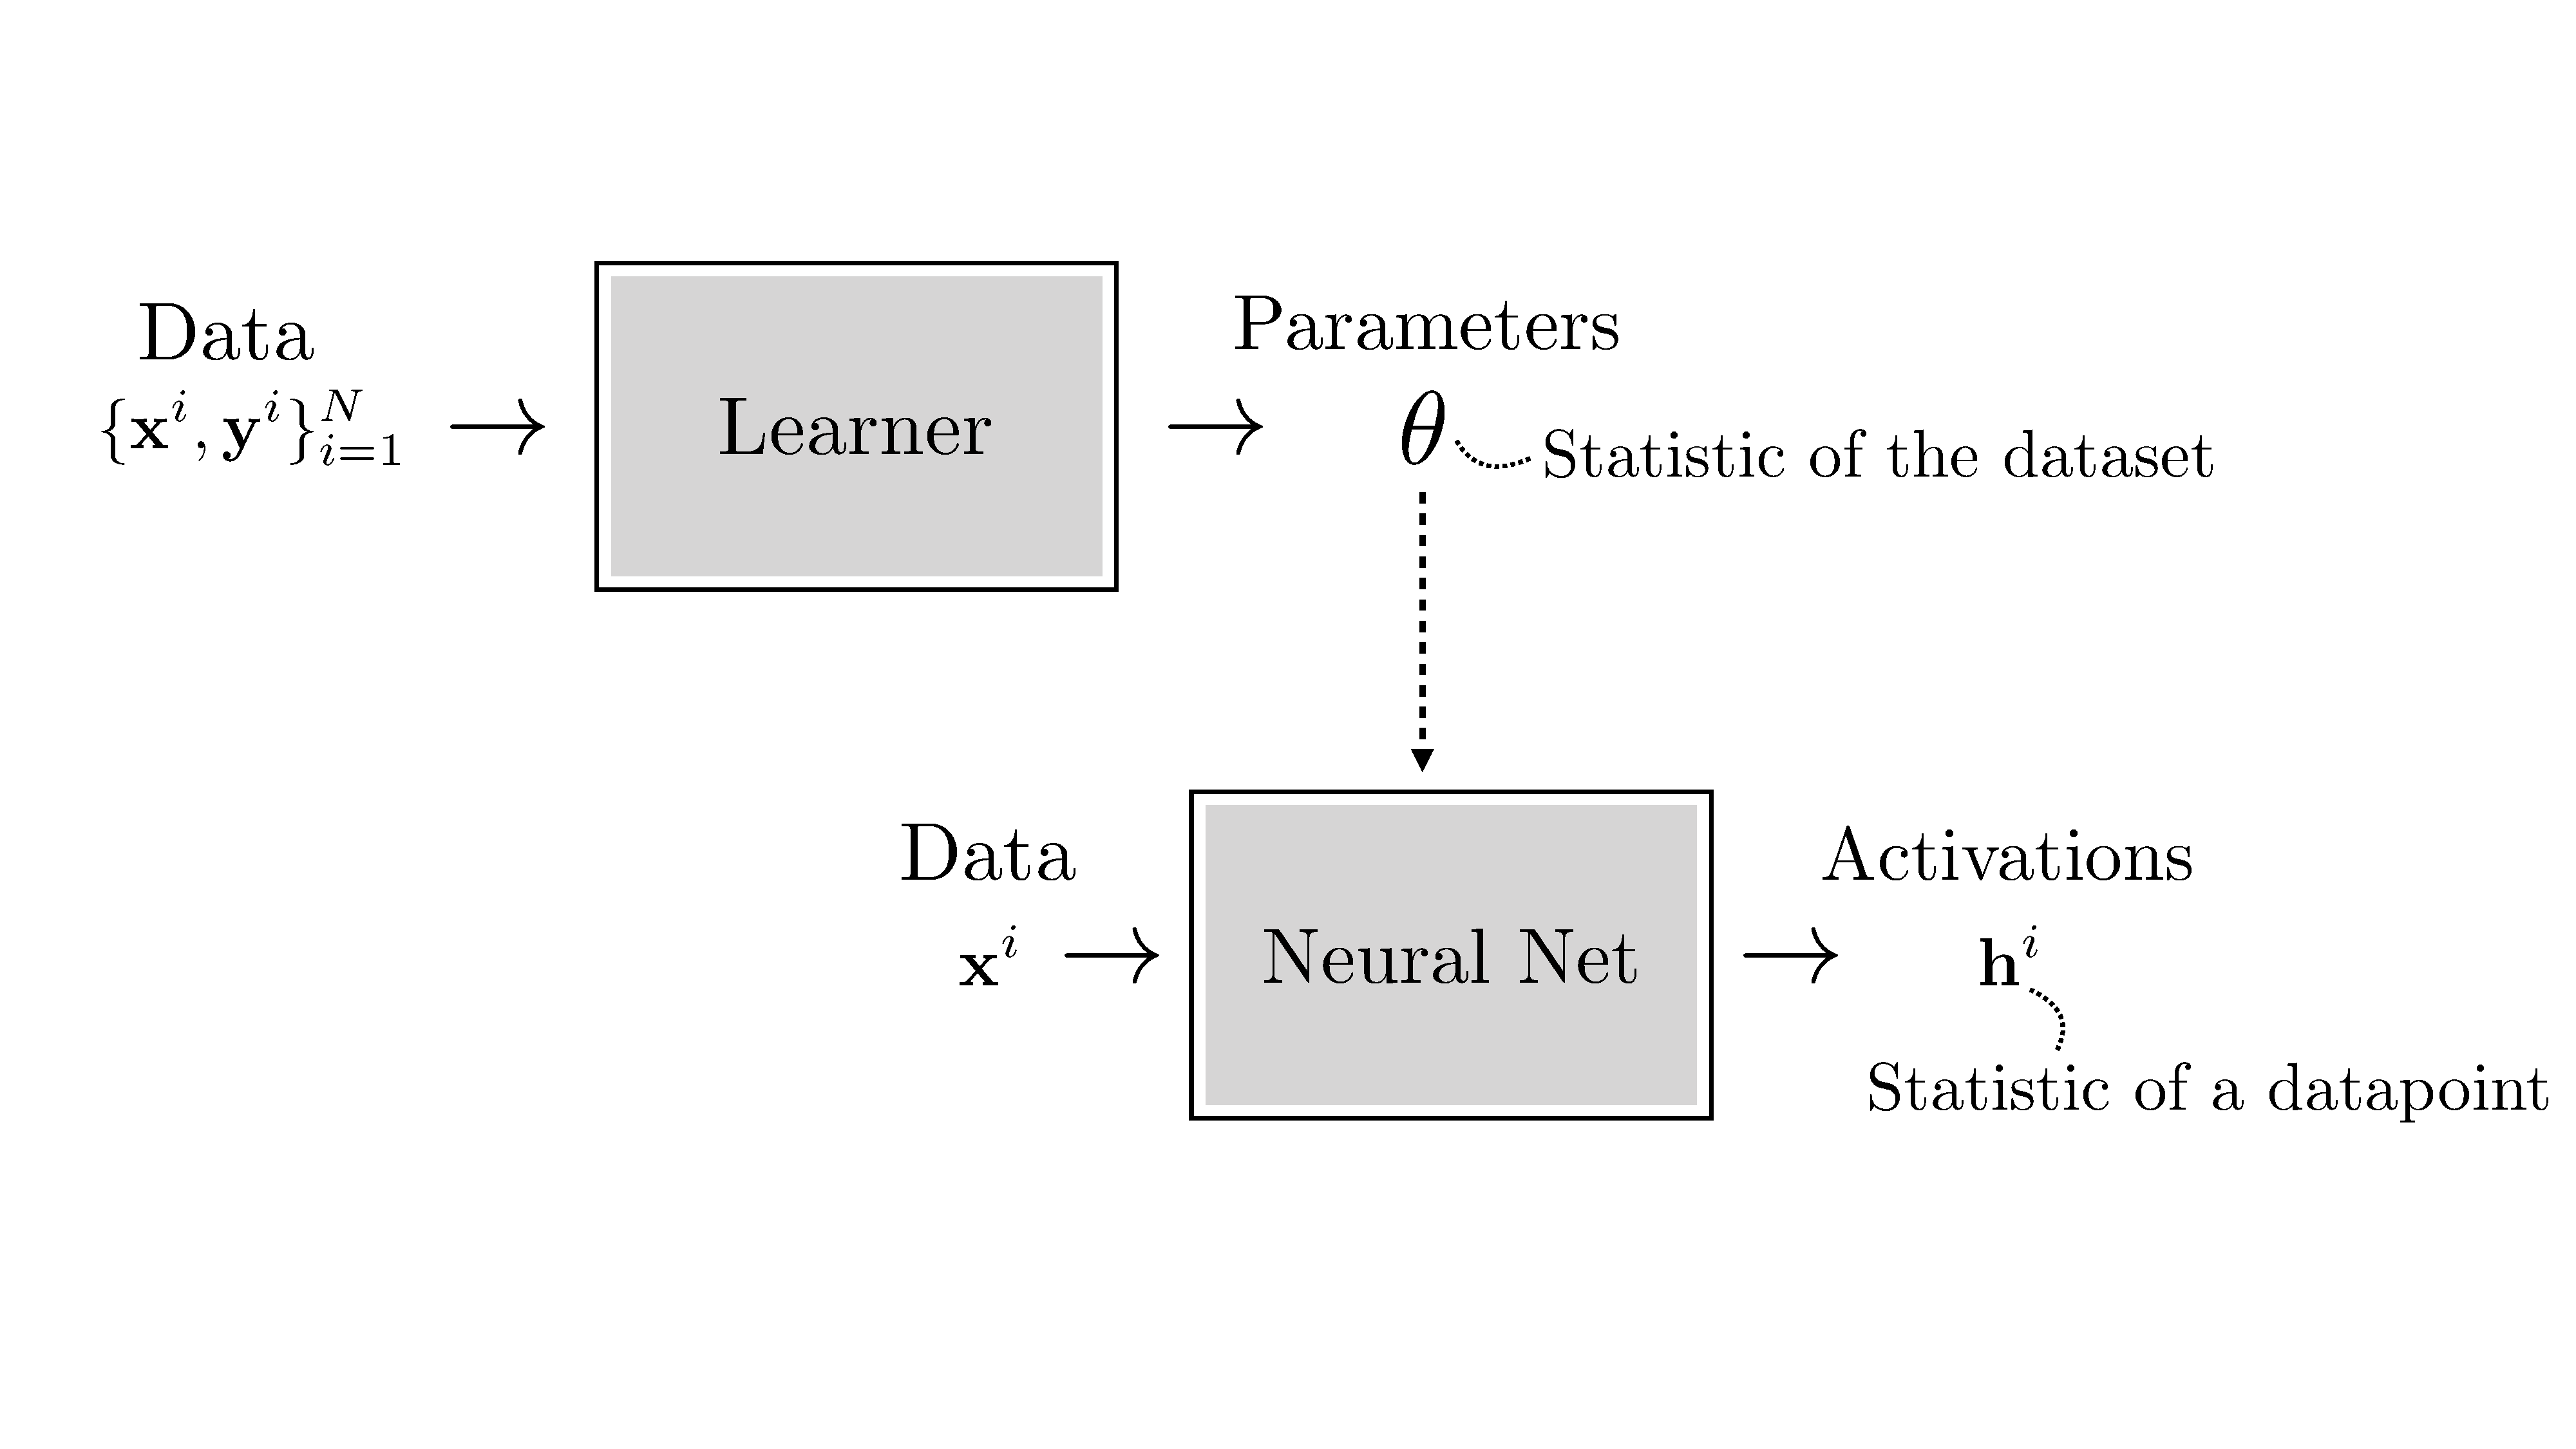
\includegraphics[width=0.7\linewidth]{figures/neural_nets/params_vs_activations.pdf}
}
\caption{Learning is a function that maps a dataset to parameters. Inference, through a neural net, is a function that maps a datapoint to activations.}
\label{fig:neural_nets:params_vs_activations}
\end{figure}

\section{Deep Nets}
Deep nets are neural nets that stack the linear-nonlinear motif many times (\fig{\ref{fig:deep_nets}}):
\begin{figure}[h]
    \centerline{
    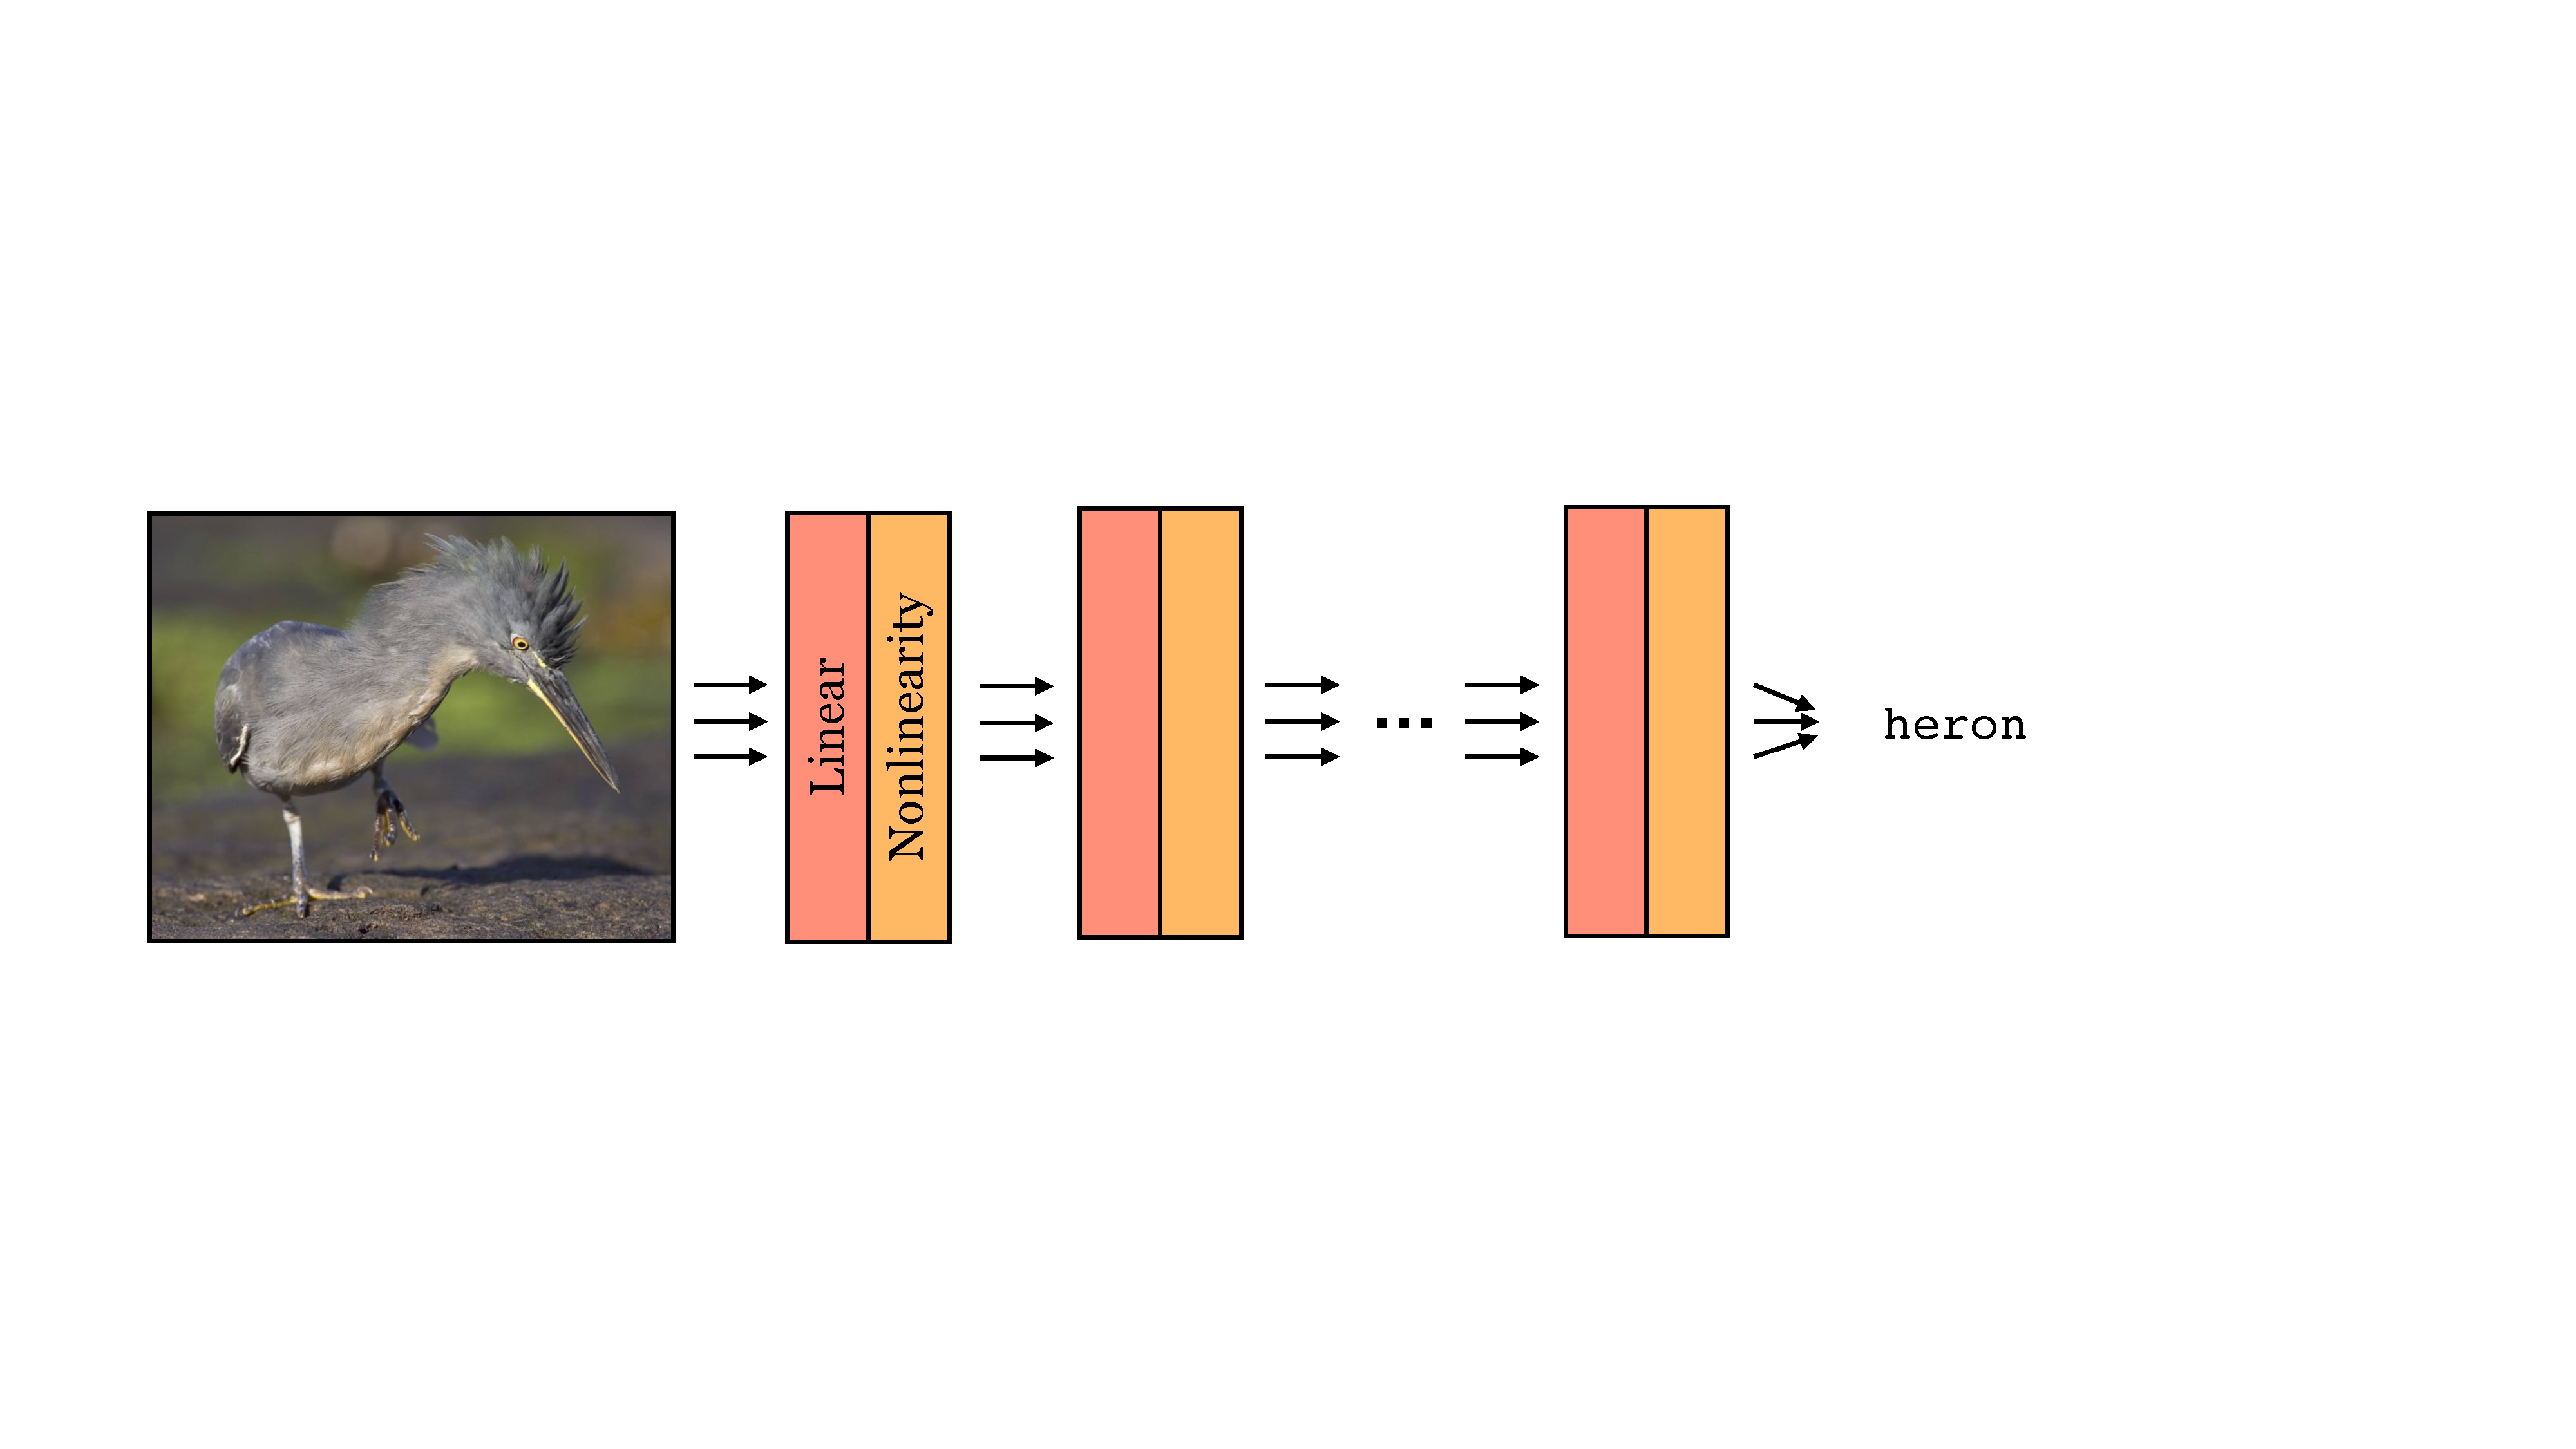
\includegraphics[width=0.65\linewidth]{./figures/neural_nets/deep_nets.pdf}
    }
    \caption{Deep nets consist of linear layers interleaved with nonlinearities.}
    \label{fig:deep_nets}
\end{figure}

Each layer is a function. Therefore, a deep net is a composition of many functions:
\begin{align}
    f(\mathbf{x}) = f_{L}(f_{L-1}(\ldots f_2(f_1(\mathbf{x}))))
\end{align}\marginnote{The $L$ is the number of layers in the net.}[-0.5cm]
These functions are parameterized by weights $[\mathbf{W}_1, \ldots, \mathbf{W}_L]$ and biases $[\mathbf{b}_1, \ldots, \mathbf{b}_L]$. Some layers we will see later have other parameters. Collectively, we will refer to the concatenation of all the parameters in a deep net as $\theta$. %A deep net with the pattern above, that simply alternates linear layers with pointwise non-linearities is called a {\bf multi-layer perceptron}, or {\bf MLP}, as it is can be considered as a set of perceptrons stacked in sequence.

Deep nets are powerful because they can perform nonlinear mappings. In fact, a deep net with sufficiently many neurons can fit almost any desired function arbitrarily closely, a property we will investigate further in \sect{\ref{sec:neural_nets:universal_approximation}}. %The {\bf universal approximation theorem}~\cite{Cybenko1989} states that this is true even for a network with just a single hidden layer. The caveat is that the number of neurons in the hidden layers will have to be very large in order to fit complicated functions. Also, technically, this theorem only holds for continuous functions on compact subsets of $\mathbb{R}^N$ -- for example a neural net cannot fit non-computable functions.


\subsection{Deep Nets Can Perform Nonlinear Classification}

Let's return to our binary classification problem shown previously, but now let's make the two classes not linearly separable. Our new dataset is shown in \fig{\ref{fig:neural_nets:nonseparable_dataset}}.
\begin{figure}[h]
\noindent\hspace{0.3\linewidth}
\begin{minipage}{0.33\linewidth}
\begin{tikzpicture}
\begin{axis}[view={0}{90}, xmin=-1, xmax=1, ymin=-1, ymax=1, 
width=1.0\linewidth, xlabel=$x_1$, ylabel=$x_2$,
align=center,
title={},
axis equal image,
x label style={at={(axis description cs:0.5,-0.17)}},
y label style={at={(axis description cs:-0.17,0.5)}},
%x label style={at={(axis description cs:0.5,0.0)}},
%y label style={at={(axis description cs:0.2,0.5)}},
scatter/classes={%
    pos_correct={mark=text, text mark={\bf 1}},%
    pos_incorrect={mark=text, text mark={\bf \color{red} 1}},%
    neg_correct={mark=text, text mark={\bf 0}},%
    neg_incorrect={mark=text, text mark={\bf \color{red} 0}}}]
%
\addplot[scatter,only marks,%
    scatter src=explicit symbolic]%
table[meta=label] {
x y label
0.1 0.3 neg_correct
0.6 0.15 neg_correct
0.4 0.5 neg_correct
-0.1 0.71 neg_correct
-0.4 0.31 neg_correct
-0.7 0.54 neg_correct
%
0.12 -0.67 pos_correct
-0.34 -0.23 neg_correct
-0.78 -0.68 neg_correct
.84 -0.2 neg_correct
-0.18 -0.5 pos_correct
0.47 -0.64 pos_correct
0.22 -0.28 pos_correct
0.7 -0.54 pos_correct
    };
\end{axis}
\end{tikzpicture}
\end{minipage}
\caption{Dataset that is not linearly separable.}
\label{fig:neural_nets:nonseparable_dataset}
\end{figure}

Here there is no line that can separate the zeros from the ones. Nonetheless, we will demonstrate a multilayer network that can solve this problem. The trick is to just add more layers! We will use the two layer MLP shown in \fig{\ref{fig:neural_nets:simple_MLP_network}}.

\begin{figure}[h]
\centerline{

\noindent\hspace{0.05\linewidth}
\begin{minipage}{.45\linewidth}

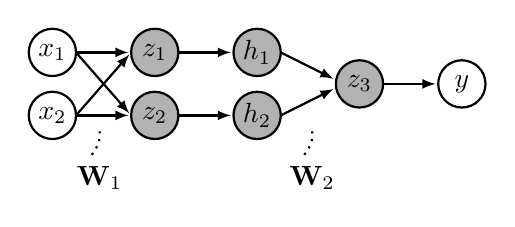
\begin{tikzpicture}[>=spaced latex]
\draw [thick] (0,-0.4) circle [radius=0.3] node {$x_2$};
\draw [thick] (0,0.4) circle [radius=0.3] node {$x_1$};
\draw [thick] [nn_edge] (0.3,-0.4) -- (1.0,-0.4);
\draw [thick] [nn_edge] (0.3,0.4) -- (1.0,0.4);
\draw [thick] [nn_edge] (0.3,-0.4) -- (1.0,0.4);
\draw [thick] [nn_edge] (0.3,0.4) -- (1.0,-0.4);
\draw [thick, fill=gray_neuron] (1.3,-0.4) circle [radius=0.3] node {$z_2$};
\draw [thick, fill=gray_neuron] (1.3,0.4) circle [radius=0.3] node {$z_1$};
\draw [thick,dotted] (0.5,-0.9)  .. controls (0.6,-0.75) .. (0.6,-0.6);
\draw (0.6,-1.2) node {$\mathbf{W}_1$};

\draw [thick] [nn_edge] (1.6,-0.4) -- (2.3,-0.4);
\draw [thick] [nn_edge] (1.6,0.4) -- (2.3,0.4);
\draw [thick, fill=gray_neuron] (2.6,-0.4) circle [radius=0.3] node {$h_2$};
\draw [thick, fill=gray_neuron] (2.6,0.4) circle [radius=0.3] node {$h_1$};
\draw [thick,dotted] (3.2,-0.9)  .. controls (3.3,-0.75) .. (3.3,-0.6);
\draw (3.3,-1.2) node {$\mathbf{W}_2$};

\draw [thick] [nn_edge] (2.9,-0.4) -- (3.6,-0.05);
\draw [thick] [nn_edge] (2.9,0.4) -- (3.6,0.05);
\draw [thick, fill=gray_neuron] (3.9,0) circle [radius=0.3] node {$z_3$};
\draw [thick] [nn_edge] (4.2,0) -- (4.9,0);
\draw [thick] (5.2,0) circle [radius=0.3] node {$y$};
\end{tikzpicture}
\caption{A simple MLP network.}
\label{fig:neural_nets:simple_MLP_network}
\end{minipage}
}
\end{figure}

Consider using the following settings for $\mathbf{W}_1$ and $\mathbf{W}_2$:
\begin{align}
    \mathbf{W}_1 = 
        \begin{bmatrix}
            -1 & 1 \\
            1 & 2
        \end{bmatrix}
    ,\quad\quad
    \mathbf{W}_2 = 
        \begin{bmatrix}
            1 & -1
        \end{bmatrix}
\end{align}
The full net then performs the following operation:
\begin{align}
    z_1 &= x_1 - x_2, \quad z_2 = 2x_1 + x_2 &\triangleleft \quad \texttt{linear}\\
    h_1 &= \max(z_1,0), \quad h_2 = \max(z_2,0) &\triangleleft \quad \texttt{relu}\\
    z_3 &= h_1-h_2 &\triangleleft \quad \texttt{linear}\\
    y &= \mathbbm{1}(z_3 > 0) &\triangleleft \quad \text{\texttt{threshold}}
\end{align}
\marginnote{The $\mathbbm{1}$ is the indicator function, which we define as: \begin{equation*}
    \mathbbm{1}(x) = \begin{cases}
                1 & \text{if $x$ is true} \\
                0 & \text{otherwise}
             \end{cases}
\end{equation*}}[-0.5cm]
Here we have introduced a new pointwise nonlinearity, the \index{Rectified linear unit}\textbf{Rectified linear unit} (\textbf{relu}), which is like a graded version of a threshold function, and has the advantage that it yields non-zero gradients over half its domain, thus being amenable to gradient-based learning.

We visualize the values that the neurons take on as a function of $x_1$ and $x_2$ in \fig{\ref{fig:neural_nets:simple_MLP_network_values}}.

\begin{figure}[h]
%\noindent\hspace{0.05\linewidth}
\begin{minipage}{1.0\linewidth}
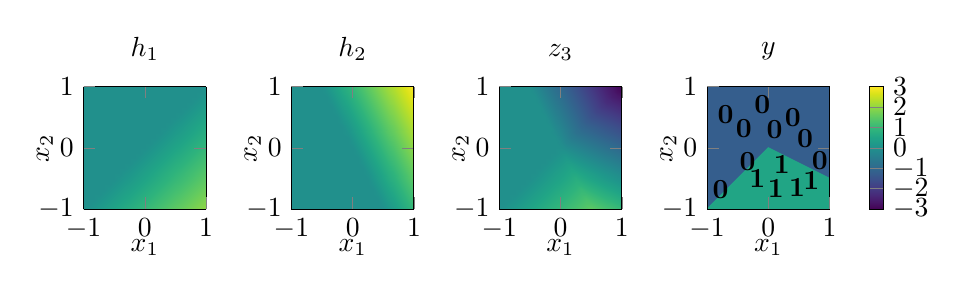
\begin{tikzpicture}
\begin{axis}[name=plot1, view={0}{90}, xmin=-1, xmax=1, ymin=-1, ymax=1, 
width=0.3\linewidth, xlabel=$x_1$, ylabel=$x_2$, 
title=$h_1$,
axis equal image,
x label style={at={(axis description cs:0.5,-0.17)}},
y label style={at={(axis description cs:-0.17,0.5)}},
point meta min=-3, point meta max=3
]
	\addplot3[surf, shader=interp, domain=-1:1] {max(-y+x,0)};
\end{axis}
\begin{axis}[name=plot2, at=(plot1.right of south east), xshift=25, view={0}{90}, xmin=-1, xmax=1, ymin=-1, ymax=1, 
width=0.3\linewidth, xlabel=$x_1$, ylabel=$x_2$, 
title=$h_2$,
axis equal image,
x label style={at={(axis description cs:0.5,-0.17)}},
y label style={at={(axis description cs:-0.17,0.5)}},
point meta min=-3, point meta max=3
]
	\addplot3[surf, shader=interp, domain=-1:1] {max(y+2*x,0)};
\end{axis}
\begin{axis}[name=plot3, at=(plot2.right of south east), xshift=25, view={0}{90}, xmin=-1, xmax=1, ymin=-1, ymax=1, 
width=0.3\linewidth, xlabel=$x_1$, ylabel=$x_2$, 
title=$z_3$,
axis equal image,
x label style={at={(axis description cs:0.5,-0.17)}},
y label style={at={(axis description cs:-0.17,0.5)}},
point meta min=-3, point meta max=3
]
	\addplot3[surf, shader=interp, domain=-1:1] {max(-y+x,0)-max(y+2*x,0)};
\end{axis}
\begin{axis}[name=plot4, at=(plot3.right of south east), xshift=25, view={0}{90}, xmin=-1, xmax=1, ymin=-1, ymax=1, 
width=0.3\linewidth, xlabel=$x_1$, ylabel=$x_2$,
title=$y$,
colorbar,
colorbar style={
        ytick={-3.0,-2.0,-1.0,0,1.0,2.0,3.0},
        yticklabel style={
            align=right
        },
        width=5.0
    },
axis equal image,
x label style={at={(axis description cs:0.5,-0.17)}},
y label style={at={(axis description cs:-0.17,0.5)}},
point meta min=-3, point meta max=3,
%ymajorticks=false
scatter/classes={%
    pos_correct={mark=text, text mark={\bf 1}},%
    pos_incorrect={mark=text, text mark={\bf \color{red} 1}},%
    neg_correct={mark=text, text mark={\bf 0}},%
    neg_incorrect={mark=text, text mark={\bf \color{red} 0}}}]
]
    \addplot3[surf, shader=interp, domain=-1:1] {max(-y+x,0)-max(y+2*x,0)};
	\addplot[fill, index of colormap={5 of viridis}, color=.] coordinates 
		{(-1,-1) (0,0) (1,-0.5) (1,1) (-1,1)} --cycle;
	\addplot[fill, index of colormap={10 of viridis}, color=.] coordinates 
		{(-1,-1) (0,0) (1,-0.5) (1,-1)} --cycle;
    \addplot[scatter,only marks,%
    scatter src=explicit symbolic]%
table[meta=label] {
x y label
0.1 0.3 neg_correct
0.6 0.15 neg_correct
0.4 0.5 neg_correct
-0.1 0.71 neg_correct
-0.4 0.31 neg_correct
-0.7 0.54 neg_correct
%
0.12 -0.67 pos_correct
-0.34 -0.23 neg_correct
-0.78 -0.68 neg_correct
.84 -0.2 neg_correct
-0.18 -0.5 pos_correct
0.47 -0.64 pos_correct
0.22 -0.28 pos_correct
0.7 -0.54 pos_correct
    };
\end{axis}
\end{tikzpicture}
\end{minipage}
\caption{Values of hidden units and output unit for the MLP shown in \fig{\ref{fig:neural_nets:simple_MLP_network}}.}
\label{fig:neural_nets:simple_MLP_network_values}
\end{figure}

As can be seen in the rightmost plot, at the output $y$, this neural net successfully assigns a value of 1 to the region of the dataspace where the datapoints labeled as 1 live. This example demonstrates that is possible to solve nonlinear classification problems with a deep net. In practice, we would want to \textit{learn} the parameter settings that achieve this classification. One way to do so would be to enumerate all possible parameter settings and pick one that successfully separates the zeros from the ones. This kind of exhaustive enumeration is a slow process, but don't worry, in \chap{\ref{chapter:backpropagation}} we will see how to speed things up using gradient descent. But it's worth remarking that enumeration is always a sufficient solution, at least when the possible parameter values form a finite set.


%\subsection{Deep nets can perform nonlinear regression}

%What about regression? It turns out deep nets are good for that too, in fact, they can be effective at implementing many kinds of functional mappings.

%Here are the functions of some random nets:

%\begin{figure}[h]
%    \centering
%    \includegraphics[width=0.19\linewidth]{figures/neural_nets/random_net1.pdf}
%    \includegraphics[width=0.19\linewidth]{figures/neural_nets/random_net2.pdf}
%    \includegraphics[width=0.19\linewidth]{figures/neural_nets/random_net3.pdf}
%    \includegraphics[width=0.19\linewidth]{figures/neural_nets/random_net4.pdf}
%    \includegraphics[width=0.19\linewidth]{figures/neural_nets/random_net5.pdf}
%    \label{fig:random_nets}
%\end{figure}

%Here's what happens as you tune one parameter. You can get it to fit all kinds of things!

\subsection{Deep Nets Are Universal Approximators}\label{sec:neural_nets:universal_approximation}
Not only can deep nets perform nonlinear classification, they can in principle perform \textit{any} continuous input-output mapping. The \index{Universal approximation theorem}{\bf universal approximation theorem}~\cite{Cybenko1989} states that this is true even for a network with just a single hidden layer. The caveat is that the number of neurons in the hidden layers will have to be very large in order to fit complicated functions.\marginnote{Technically, this theorem only holds for continuous functions on compact subsets of $\mathbb{R}^N$ -- for example a neural net cannot fit noncomputable functions. We will not be rigorous in this section. We direct the reader to \cite{TelgarskyNotes2021} for a formal treatment of universal approximation.}[-1.4cm]
%As mentioned above, this is only true if we assume the net can have an arbitrary large number of neurons. In this section we will give an intuition for why this is true.

To get an intuition for why this is true, we will consider the case of approximating an arbitrary function from $\mathbb{R} \rightarrow \mathbb{R}$ with a relu-MLP (an MLP with relu nonlinearities). First observe that any function can be approximated arbitrarily well by a sum of indicator functions, that is, bumps placed at different positions:
\begin{align}
    f(x) \approx \sum_i w_i \mathbbm{1}(\alpha_i < x < \beta_i)\label{eqn:neural_nets:sum_of_indicators}
\end{align}
As an example, in \fig{\ref{fig:neural_nets:curve_as_bump}} we show a curve (blue line) approximated in this way. As the width, $\beta-\alpha$, of the bumps (black lines) goes to zero, the error in the fit goes to zero.
\begin{figure}[h]
    \centerline{
    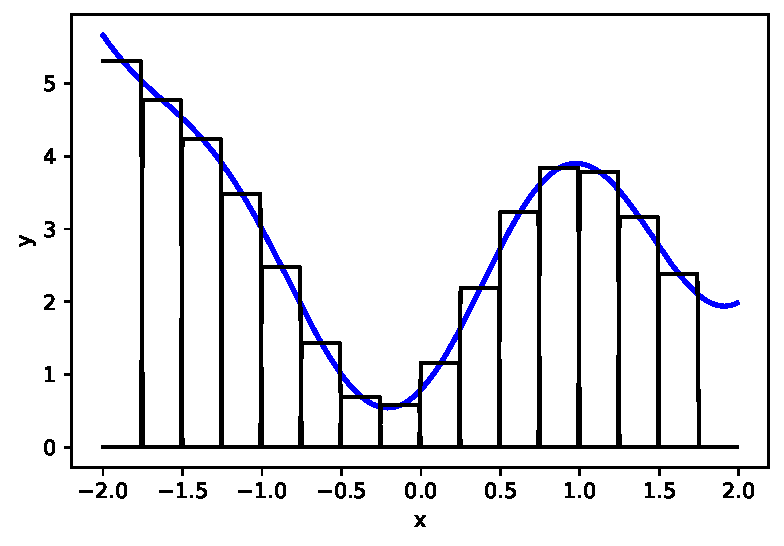
\includegraphics[width=0.35\linewidth]{./figures/neural_nets/curve_as_bumps.pdf}
    }
    \caption{Any function from $\mathbb{R} \rightarrow \mathbb{R}$ can be approximated arbitrarily well by a sum of elementary bumps.}
    \label{fig:neural_nets:curve_as_bump}
\end{figure}

\marginnote{While we only consider scalar functions $\mathbb{R} \rightarrow \mathbb{R}$ here, a similar construction can be used to approximate general functions of the form $\mathbb{R}^n \rightarrow \mathbb{R}^m$.}[-1.8cm]

Next we will show that a relu-MLP can represent \eqn{\ref{eqn:neural_nets:sum_of_indicators}}. The weighted sum $\sum_i w_i \ldots$ is the easy part: that's just a linear layer. So we just have to show that we can also write $\mathbbm{1}(\alpha < x < \beta)$ using linear and relu layers. It turns out the construction is rather simple:
\begin{align}
\mathbbm{1}(\alpha < x < \beta) \approx \texttt{relu}\bigg(\frac{x-(\alpha-\gamma)}{\gamma}\bigg) - \texttt{relu}\bigg(\frac{x-\alpha}{\gamma}\bigg) - \texttt{relu}\bigg(\frac{x-(\beta-\gamma)}{\gamma}\bigg) + \texttt{relu}\bigg(\frac{x-\beta)}{\gamma}\bigg) \label{eqn:neural_nets:bump_as_relu_net}
\end{align}
\marginnote{Here we show how a neural net can represent a function as a sum of basis functions. This idea is also foundational in signal processing, where signals are often represented as a sum of sine waves (\chap{\ref{chapter:fourier_analysis}}), boxes (\fig{\ref{fig:upsampling_and_downsampling:nn_interp}}), or trapezoids (\fig{\ref{fig:bilinear_interp}}).}[-2.0cm]
As $\gamma \rightarrow 0$, this approximation becomes exact. The input to each of the four relus in \eqn{\ref{eqn:neural_nets:bump_as_relu_net}} is an affine function of the input $x$, hence these four values can be represented by a linear layer with four outputs. Then we apply a relu layer to these four values, and finally we apply a linear layer to compute the sum over these relus (a weighted sum with weights [1,-1,-1,1]). Therefore \eqn{\ref{eqn:neural_nets:bump_as_relu_net}} can be implemented as a \texttt{linear}-\texttt{relu}-\texttt{linear} network. In \fig{\ref{fig:neural_nets:bump_as_relus}}, we show an example of constructing a bump in this way.
\begin{figure}[h]
    \centerline{
    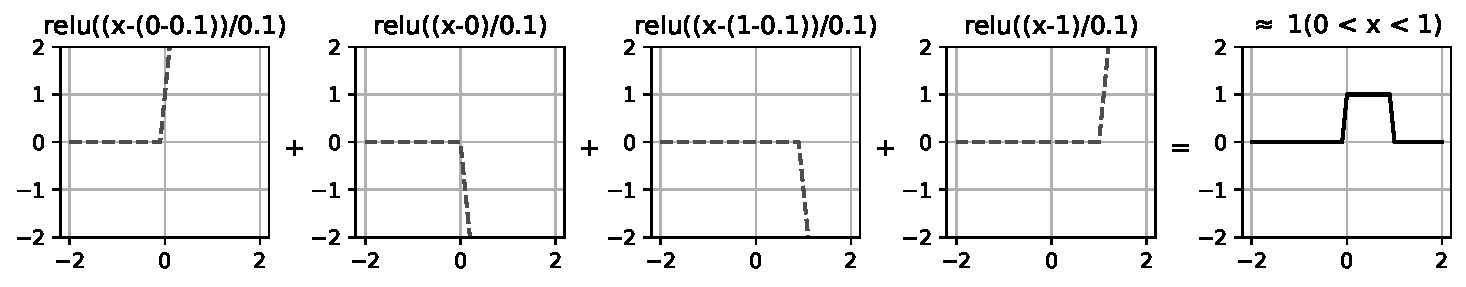
\includegraphics[width=1.0\linewidth]{./figures/neural_nets/bump_as_relus.pdf}
    }
    \caption{A bump can be represented as a weighted sum of shifted and scaled relu functions.}
    \label{fig:neural_nets:bump_as_relus}
\end{figure}

Putting everything together, we have a \texttt{linear}-\texttt{relu}-\texttt{linear} for each bump, followed by a linear layer for summing up all the bumps. The two linear layers in sequence can be collapsed to a single linear layer, and hence the full function can therefore be approximated, to arbitrary precision, by a \texttt{linear}-\texttt{relu}-\texttt{linear} net.\marginnote{Most literature refers to such a net as having a single hidden layer, using the convention that we don't count pre- and postactivation neurons as separate layers.}

%The inputs to each of these $\texttt{relu}$ functions can be implemented as a linear layer (a scaling + bias), so the whole network that approximates a function as a sum of bumps is simply a linear-relu-linear net, i.e. a net with a single hidden layer. 

Notice that in this approximation, we need four relu neurons for each bump we are modeling. Therefore if we want to approximate a very bumpy function, say with $N$ bumps, we will need $4N$ relu neurons. In general, to achieve arbitrarily good approximation to a curve we may need an unbounded number of neurons in our network.

\subsection{Depth versus Width}
Above we saw that if you have a hidden layer with $N$ neurons, you can fit a scalar function with $\mathcal{O}(N)$ bumps. The number of neurons on a single hidden layer is called its \index{Network width}\textbf{width}.\marginnote{If different layers have different numbers of neurons, then we may specify the width per layer. Here we will assume all layers have the same width and simply speak of the width of the network.}[-0.4cm] So, as we increase the width of a network, we can fit ever more complicated functions. What if we instead increase the \index{Network depth}\textbf{depth} of a network, that is, its number of layers? It turns out that this can also be an effective way to increase the capacity of the net, but its effect is a bit different than increasing width.

Interestingly, it is sometimes the case that \textit{deep} nets require far fewer parameters to fit data than \textit{wide} nets. Evidence for this statement comes mostly from empiricism, where researchers have found that deeper nets just work better in practice on many popular problems. However, there is also the beginning of a mathematical theory of when and why this can happen. The basic idea of this theory is to establish that there are certain classes of function that can be represented with a polynomial number of neurons in a depth $d$ network but require an exponential number of neurons in a depth $d^\prime$ network, for certain $d^\prime < d$. Arguments along these lines are called \textbf{depth separations}, and the interested reader can refer to \cite{telgarsky2016benefits} to learn more about this ongoing line of research.

%The above argument shows that relu networks can approximate any function. There is a great deal of additional theory on exactly how many units and layers are needed to approximate exactly what kind of functions to exactly what degree of precision. One important result in this direction is Barron's theorem~\cite{barron1993universal}.

%Chapter \ref{chapter:intro_to_learning}
\section{Deep Learning: Learning with Neural Nets}
Using the formalism we defined in \chap{\ref{chapter:intro_to_learning}}, learning consists of using an \emph{optimizer} to find a function in a \emph{hypothesis space}, that maximizes an \emph{objective}. From this perspective, neural nets are simply a special kind of hypothesis space (and a particular parameterization of that hypothesis space). \index{Deep learning}\textbf{Deep learning} refers to learning algorithms that use this parameterized hypothesis space.

Deep learning also typically involves using gradient-based optimization to search the hypothesis space for the best fit to the data. We will investigate this approach in detail in \chap{\ref{chapter:backpropagation}}, where we will learn about the \textbf{backpropagation} algorithm for gradient-based learning with neural nets. However, it is certainly possible to optimize neural nets with other methods, including zeroth-order optimizers like evolution strategies (\sect{\ref{sec:gradient_descent:zeroth_order}}; \cite{salimans2017evolution}). 

One intriguing alternative to backpropagation is called \index{Hebbian learning}\textbf{Hebbian learning}~\cite{hebb2005organization}. Backpropagation is a \textit{top-down} learning algorithm, where errors incurred at the output (top) of the net are propagated backward to inform earlier layers how to update their weights and biases to minimize the loss, which is a form of learning based on \textit{feedback}. Hebbian learning, in contrast, is a \textit{bottom-up} approach, where neurons wire up just based on the \textit{feedforward} pattern of activity in the net. The canonical learning rule in Hebbian methods is \textbf{Hebb's rule}: ``fire together, wire together.'' That is, we increase the weight of the connection between two neurons whenever the two neurons are active at the same time. Although this learning rule is not explicitly minimizing a loss function, it has been shown to lead to effective neural representations. For example, Hebb-like rules can learn \textbf{infomax} representations, which capture, in the neural activations, as much information as possible about the input signal~\cite{linsker1988self}. Similar rules lead to networks that act like memory banks~\cite{hopfield1982neural}. Hebbian learning is also of interest because it is considered to be more biologically plausible than backpropagation. This is because Hebb's rule can be computed \textit{locally}—each neuron strengthens and weakens its weights based just on the activity of adjacent neurons—whereas backpropagation requires global coordination throughout the neural network. It is currently unknown how this global coordination can be achieved in biological brains.

%Indeed, it is not clear if biological neural nets actually use backpropagation. 

%Alternative optimizers include genetic algorithms~\cite{XX}, simulated annealing~\cite{XX}, and various other kinds of ``random search"~\cite{XX}.

%There is also a broad literature on ``bottom up learning rules" that do not explicitly optimize any objective (though they may implicitly). One such rule, called {\bf Hebbian learning}~\cite{hebb2005organization}, is ``fire together, wire together", that is, we increase the weight of the connection between two neurons whenever the two neurons are active at the same time.
%\marginnote{Remember, you can always just enumerate all possible parameter settings, try each, and pick the best --  smarter optimization is only about making this search faster.}

%\subsection{Classification with a deep net}
%We will now work through an example.


%\section{Regularization in neural nets}
%Weight decay, dropout


\subsection{Data Structures for Deep Learning: Tensors and Batches}

The main data structure that we will encounter in deep learning is the \index{Tensor}{\bf tensor}, which is just a multidimensional array. This may seem simple, but it's important to get comfortable with the conventions of tensor processing.

In general, everything in deep learning is represented as tensors—the input is one tensor, the activations are tensors, the weights are tensors, the outputs are tensors. If you have data that is not natively represented as a tensor, the first step, before feeding it to a deep net, is to convert it into a tensor format. Most often we use tensor of real numbers, that is, the elements of the tensor are in $\mathbb{R}$.

Suppose we have a dataset $\{\mathbf{x}^{(i)}, \mathbf{y}^{(i)}\}_{i=1}^N$ of images $\mathbf{x}$ and labels $\mathbf{y}$. The tensor way of thinking about such a dataset is as two tensors, $\mathbf{X} \in \mathbb{R}^{N \times C_0 \times H \times W }$ and $\mathbf{Y} \in \mathbb{R}^{N \times K}$. The first dimension of the tensor is the number of elements in our dataset. The remaining dimensions are the dimensionality of the images ($C_0$ color channels by height $H$ by width $W$) and labels ($K$-way classification).

The activations in the network are also tensors. For the MLP networks we have seen so far, the activation tensors have shape $N \times C_{\ell}$, where $C_{\ell}$ is the number of neurons on layer $\ell$, sometimes also called \textbf{channels} in analogy to the color channels of the input image. In later chapters we will encounter other architectures where the activation layers have additional dimensions, for example, in convolutional networks we will see activation layers that are of shape $N \times C_{\ell} \times H_{\ell} \times W_{\ell}$.

One other important concept is \index{Batch processing}{\bf batch processing}. Normally, we don't process one image at a time through a neural net. Instead we run a \textit{batch} of images all at once, and they are processed in parallel. A batch sampled from the training data can be denoted as $\{\mathbf{x}_{\texttt{batch}}^{(i)}, \mathbf{y}_{\texttt{batch}}^{(i)}\}_{i=1}^{N_{\texttt{batch}}}$, and the batch represented as a tensor has shape $\mathbf{X} \in \mathbb{R}^{N_{\texttt{batch}} \times C_0 \times H \times W}$ and $\mathbf{Y} \in \mathbb{R}^{N_{\texttt{batch}} \times K}$.

The weights and biases of the net are also usually represented as tensors. The weights and biases of a linear layer will be tensors of shape $\mathbf{W}_{\ell} \in \mathbb{R}^{C_{\ell+1} \times C_{\ell}}$ and $\mathbf{b}_{\ell} \in \mathbb{R}^{C_{\ell+1}}$.

As an example, in \fig{\ref{fig:neural_nets:simple_MLP_network_tensors_and_batches}} below, we visualize all the tensors associated with a batch of three datapoints being processed by the MLP from \fig{\ref{fig:neural_nets:simple_MLP_network}}. For this network, the input is not a set of images but instead a set of vectors $\mathbf{X} \in \mathbb{R}^{N_{\texttt{batch}} \times C_0}$. The output is one value for each input vector, so we have $\mathbf{Y} \in \mathbb{R}^{N_{\texttt{batch}} \times 1}$.

\begin{figure}[h]
\centerline{

\noindent\hspace{0.05\linewidth}
\begin{minipage}{0.65\linewidth}
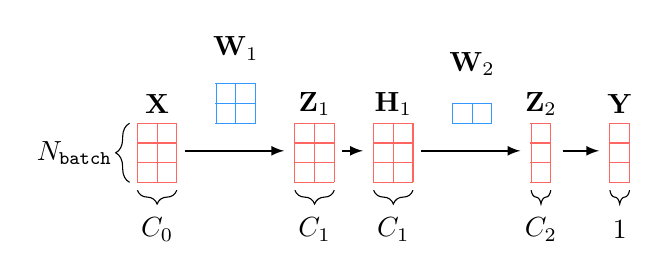
\begin{tikzpicture}
\draw[step=0.25cm,color=data_color_dark] (0,0) grid (0.5,0.75);
\draw [decorate,decoration={brace,amplitude=5pt}] (-0.1,0) -- (-0.1,0.75) node [black,midway,xshift=-0.7cm] {$N_{\texttt{batch}}$};
\draw [decorate,decoration={brace,mirror,amplitude=5pt}] (0,-0.1) -- (0.5,-0.1) node [black,midway,yshift=-0.5cm] {$C_0$};
\node at (0.25,1.0) {$\mathbf{X}$}; \draw [thick] [nn_edge] (0.6,0.4) -- (1.9,0.4);
\draw[step=0.25cm,color=param_color_dark] (0.99,0.749) grid (1.5,1.25); \node at (1.25,1.7) {$\mathbf{W}_1$};
\draw[step=0.25cm,color=data_color_dark] (1.99,0) grid (2.5,0.75); 
\draw [decorate,decoration={brace,mirror,amplitude=5pt}] (2.0,-0.1) -- (2.5,-0.1) node [black,midway,yshift=-0.5cm] {$C_1$};
\node at (2.25,1.0) {$\mathbf{Z}_1$}; \draw [thick] [nn_edge] (2.6,0.4) -- (2.9,0.4);
\draw[step=0.25cm,color=data_color_dark] (2.99,0) grid (3.5,0.75); 
\draw [decorate,decoration={brace,mirror,amplitude=5pt}] (3.0,-0.1) -- (3.5,-0.1) node [black,midway,yshift=-0.5cm] {$C_1$};
\node at (3.25,1.0) {$\mathbf{H}_1$}; \draw [thick] [nn_edge] (3.6,0.4) -- (4.9,0.4);
\draw[step=0.25cm,color=param_color_dark] (3.99,0.749) grid (4.5,1.0); \node at (4.25,1.5) {$\mathbf{W}_2$};
\draw[step=0.25cm,color=data_color_dark] (4.99,0) grid (5.25,0.75); 
\draw [decorate,decoration={brace,mirror,amplitude=5pt}] (5.0,-0.1) -- (5.25,-0.1) node [black,midway,yshift=-0.5cm] {$C_2$};
\node at (5.125,1.0) {$\mathbf{Z}_2$}; \draw [thick] [nn_edge] (5.4,0.4) -- (5.9,0.4);
\draw[step=0.25cm,color=data_color_dark] (5.99,0) grid (6.25,0.75); 
\draw [decorate,decoration={brace,mirror,amplitude=5pt}] (6.0,-0.1) -- (6.25,-0.1) node [black,midway,yshift=-0.5cm] {$1$};
\node at (6.125,1.0) {$\mathbf{Y}$};
\end{tikzpicture}
\end{minipage}
}
\caption{The tensors that represent one pass through the MLP in \fig{\ref{fig:neural_nets:simple_MLP_network}}.}
\label{fig:neural_nets:simple_MLP_network_tensors_and_batches}
\end{figure}
where the capital letters are the batches of datapoints and activations corresponding to the lowercase names of datapoints and hidden units in \fig{\ref{fig:neural_nets:simple_MLP_network}}.

This example shows the basic concept of working with tensors and batches for one-dimensional data, but, in vision, most of the time we will be working with higher-dimensional tensors. For image data we typically use four-dimensional tensors: batch $\times$ channels $\times$ height $\times$ width; for videos we may use five-dimensional tensors: batch $\times$ channels $\times$ height $\times$ width $\times$ time. Three-dimensional (3D) scans have an additional \textit{depth} spatial dimension; videos of 3D data could therefore be represented by six-dimensional tensors. As you can see, thinking in terms of two-dimensional matrices is not quite sufficient. Instead, you should be imagining data processing as operating on $N$-dimensional tensors, sliced and diced in different ways. As a step in this direction, you may find it useful to visualize tensors in 3D, as shown in \fig{\ref{fig:neural_nets:3D_tensor_example}}.
\begin{figure}[h]
\centerline{
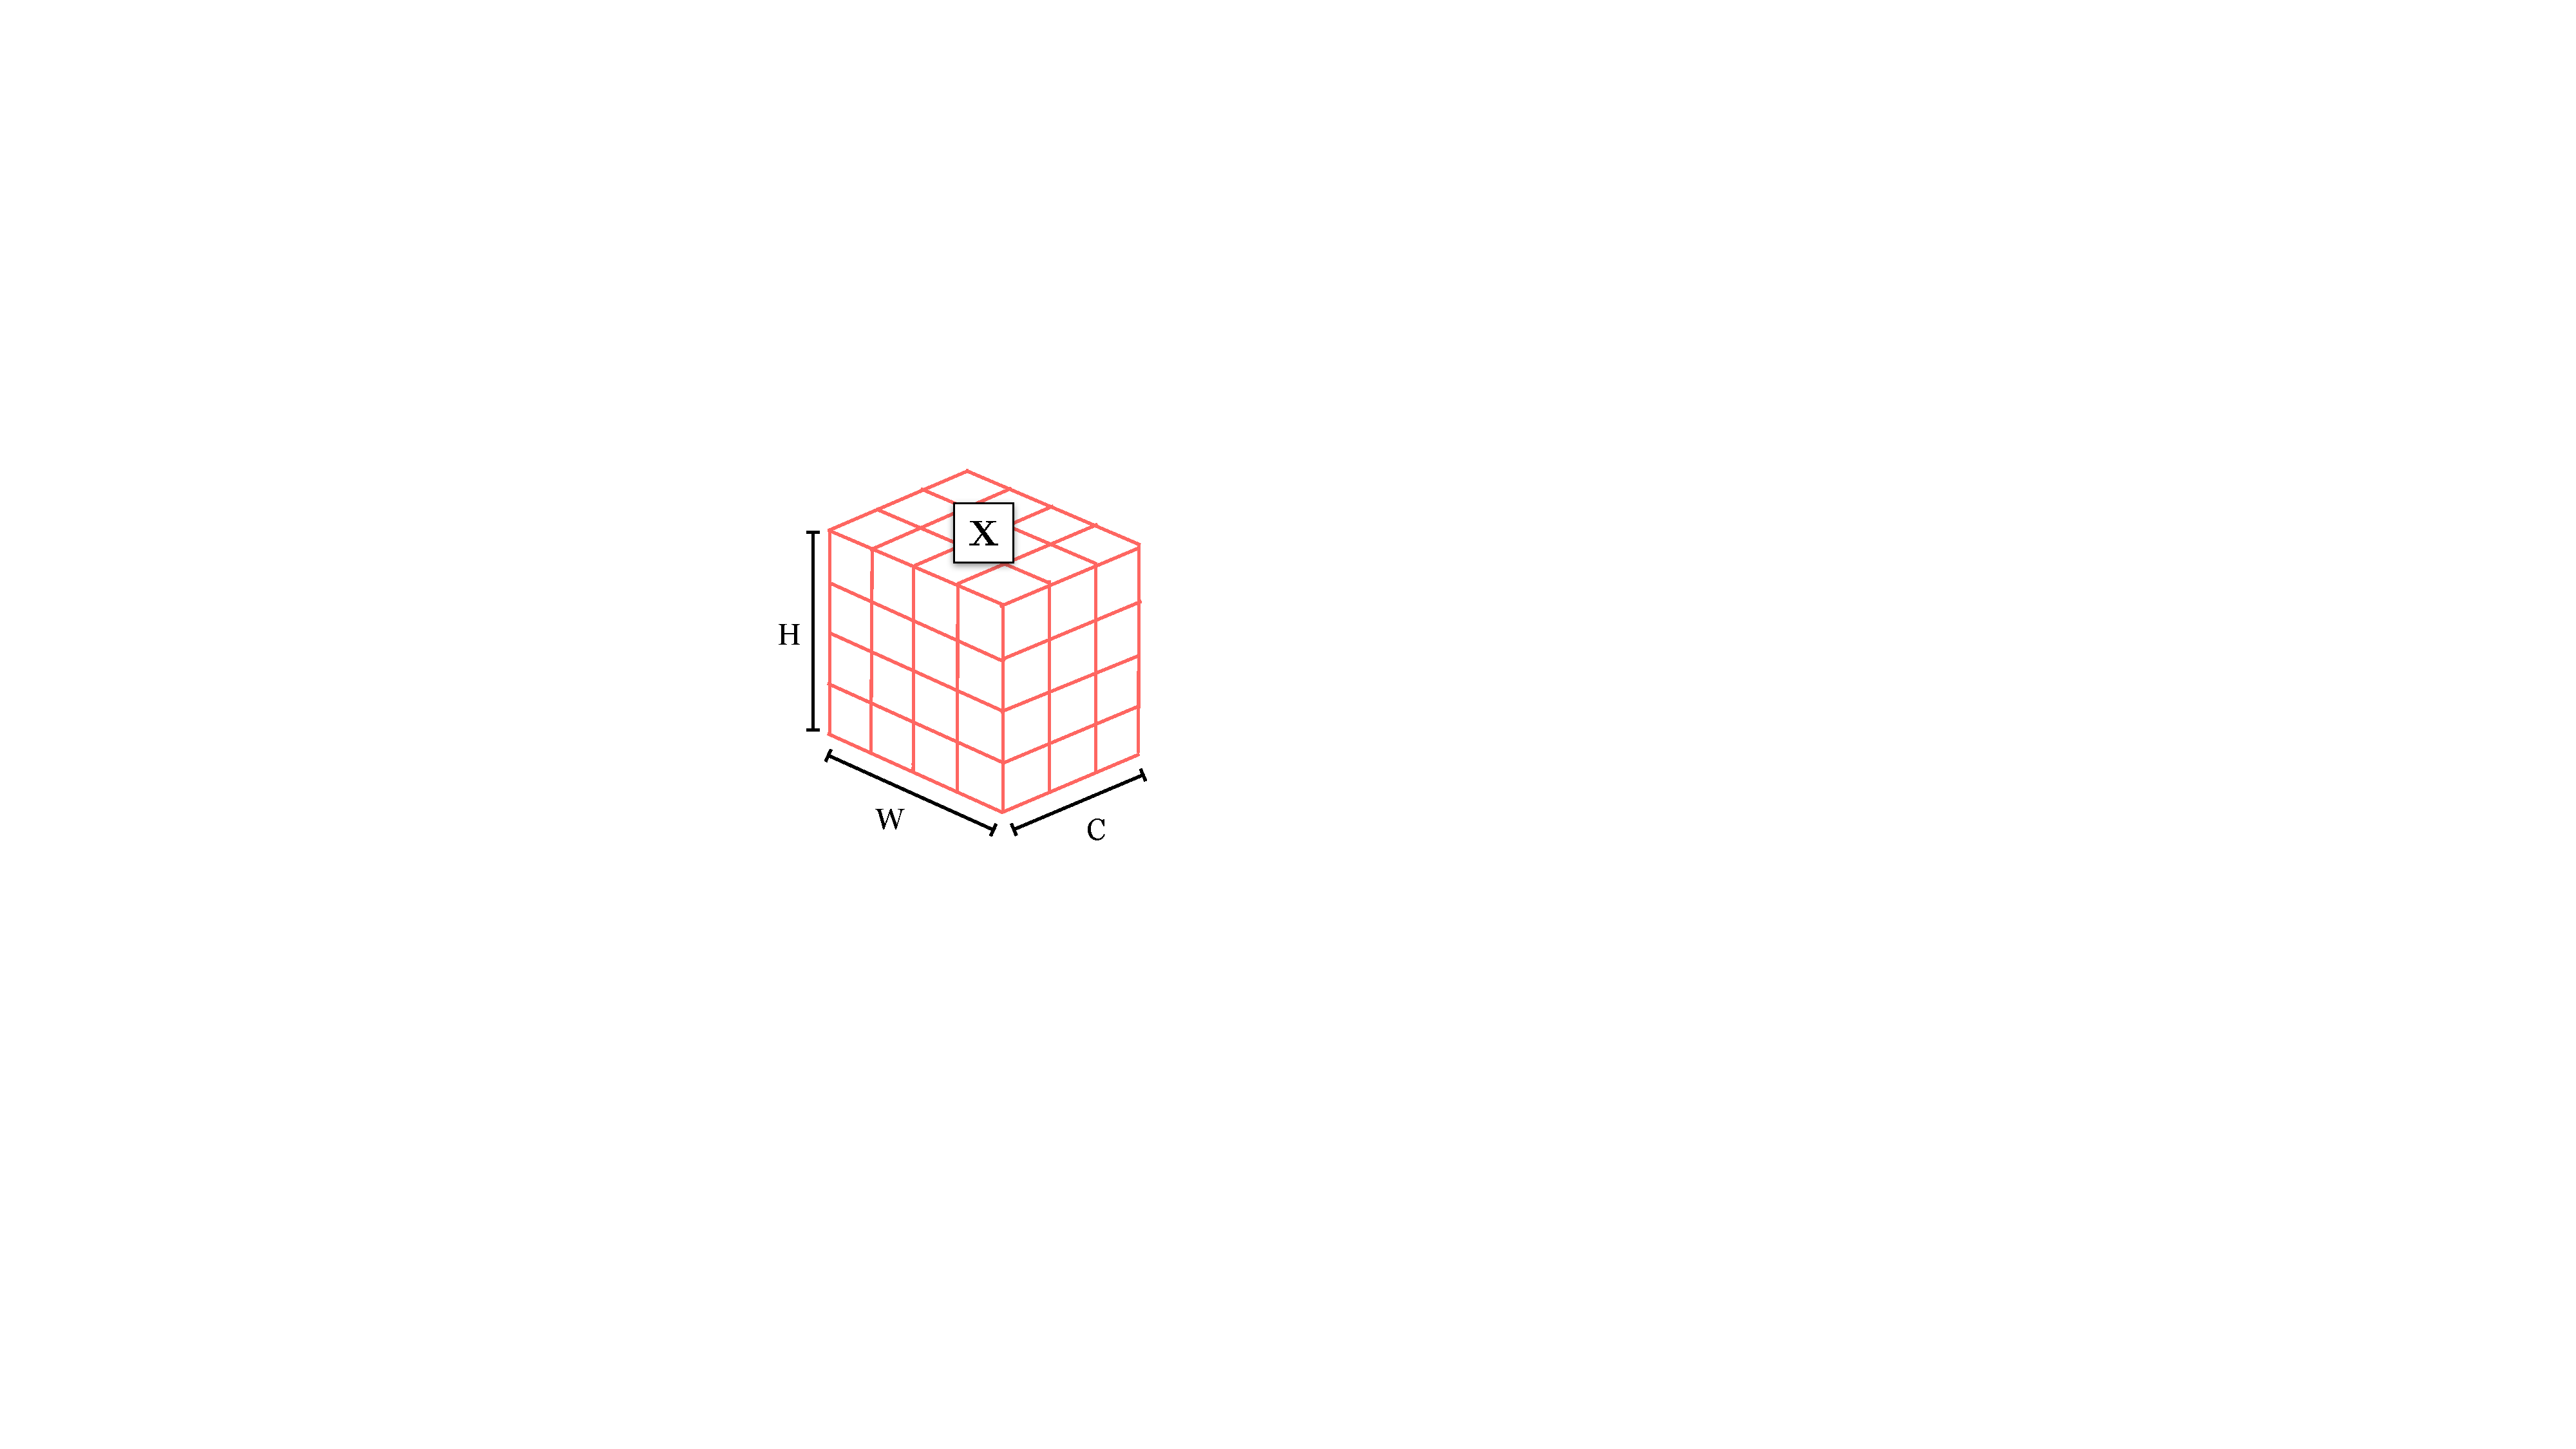
\includegraphics[width=0.2\linewidth]{figures/neural_nets/3D_tensor_example.pdf}
}
\caption{A 3D tensor that could represent an $C \times H \times W$ color image.}
\label{fig:neural_nets:3D_tensor_example}
\end{figure}

This is closer to the actual ND tensors vision systems work with, and many concepts can be adequately captured just by thinking in 3D. We will see some examples in later chapters.

% \subsection{Batch learning}
% To train a deep net we run a batch of data through it, and then compute the loss summed (or averaged) across the batch. This scores how good the current parameter settings of the network are, as estimated on a batch of training data. We can then update the parameters (e.g., at random, or with gradient descent, which we will see in the next chapter) and try again to get a better score on the next data batch. The computational pipeline, visualized as data tensors being transformed layer by layer, looks like this:

% \noindent\hspace{0.05\linewidth}
% \begin{minipage}{0.75\linewidth}
% \begin{tikzpicture}
% \draw[step=0.25cm,color=data_color] (0,3.99) grid (0.5,4.75); \node at (0.25,5.0) {$\mathbf{X}$}; \draw [thick] [nn_edge] (0.6,4.4) -- (1.9,4.4);
% \draw[step=0.25cm,color=data_color] (1.99,3.99) grid (2.5,4.75); \node at (2.25,5.0) {$\mathbf{Z}_1$}; \draw [thick] [nn_edge] (2.6,4.4) -- (2.9,4.4);
% \draw[step=0.25cm,color=data_color] (2.99,3.99) grid (3.5,4.75); \node at (3.25,5.0) {$\mathbf{H}_1$}; \draw [thick] [nn_edge] (3.6,4.4) -- (4.9,4.4);
% \draw[step=0.25cm,color=data_color] (4.99,3.99) grid (5.25,4.75); \node at (5.125,5.0) {$\mathbf{Z}_2$}; \draw [thick] [nn_edge] (5.4,4.4) -- (5.9,4.4);
% \draw[step=0.25cm,color=data_color] (5.99,3.99) grid (6.25,4.75); \node at (6.125,5.0) {$\mathbf{Y}$};
% %
% \draw[step=0.25cm,color=data_color] (0,1.99) grid (0.5,2.75); \node at (0.25,3.0) {$\mathbf{X}$}; \draw [thick] [nn_edge] (0.6,2.4) -- (1.9,2.4);
% \draw[step=0.25cm,color=data_color] (1.99,1.99) grid (2.5,2.75); \node at (2.25,3.0) {$\mathbf{Z}_1$}; \draw [thick] [nn_edge] (2.6,2.4) -- (2.9,2.4);
% \draw[step=0.25cm,color=data_color] (2.99,1.99) grid (3.5,2.75); \node at (3.25,3.0) {$\mathbf{H}_1$}; \draw [thick] [nn_edge] (3.6,2.4) -- (4.9,2.4);
% \draw[step=0.25cm,color=data_color] (4.99,1.99) grid (5.25,2.75); \node at (5.125,3.0) {$\mathbf{Z}_2$}; \draw [thick] [nn_edge] (5.4,2.4) -- (5.9,2.4);
% \draw[step=0.25cm,color=data_color] (5.99,1.99) grid (6.25,2.75); \node at (6.125,3.0) {$\mathbf{Y}$};
% %
% \draw[step=0.25cm,color=data_color] (0,0) grid (0.5,0.75); \node at (0.25,1.0) {$\mathbf{X}$}; \draw [thick] [nn_edge] (0.6,0.4) -- (1.9,0.4);
% \draw[step=0.25cm,color=data_color] (1.99,0) grid (2.5,0.75); \node at (2.25,1.0) {$\mathbf{Z}_1$}; \draw [thick] [nn_edge] (2.6,0.4) -- (2.9,0.4);
% \draw[step=0.25cm,color=data_color] (2.99,0) grid (3.5,0.75); \node at (3.25,1.0) {$\mathbf{H}_1$}; \draw [thick] [nn_edge] (3.6,0.4) -- (4.9,0.4);
% \draw[step=0.25cm,color=data_color] (4.99,0) grid (5.25,0.75); \node at (5.125,1.0) {$\mathbf{Z}_2$}; \draw [thick] [nn_edge] (5.4,0.4) -- (5.9,0.4);
% \draw[step=0.25cm,color=data_color] (5.99,0) grid (6.25,0.75); \node at (6.125,1.0) {$\mathbf{Y}$};
% \end{tikzpicture}
% \end{minipage}


\section{Catalog of Layers}
Below, we use the color blue to denote \textcolor{param_color_dark}{\bf parameters} and the color red to denote \textcolor{data_color_dark}{\bf data/activations} (inputs and outputs to each layer).
\marginnote{We color equations in this way only in this chapter, to make clear the roles of different variables. However, be on the lookout for these colors in figures later in the book. We will often draw activations in red and parameters in blue.}[-0.4cm]

\subsection{Linear Layers}
Linear layers are the workhorses of deep nets. Almost all parameters of the network are contained in these layers; we call these parameters the weights and biases. We have already introduced linear layers previously. They look like this:
\begin{align}
    \textcolor{data_color_dark}{\xout} = \textcolor{param_color_dark}{\mathbf{W}} \textcolor{data_color_dark}{\xin} + \textcolor{param_color_dark}{\mathbf{b}} & \quad\quad \triangleleft \quad\texttt{linear}
\end{align}

\subsection{Activation Layers}

\begin{figure}[t]
    \centerline{
    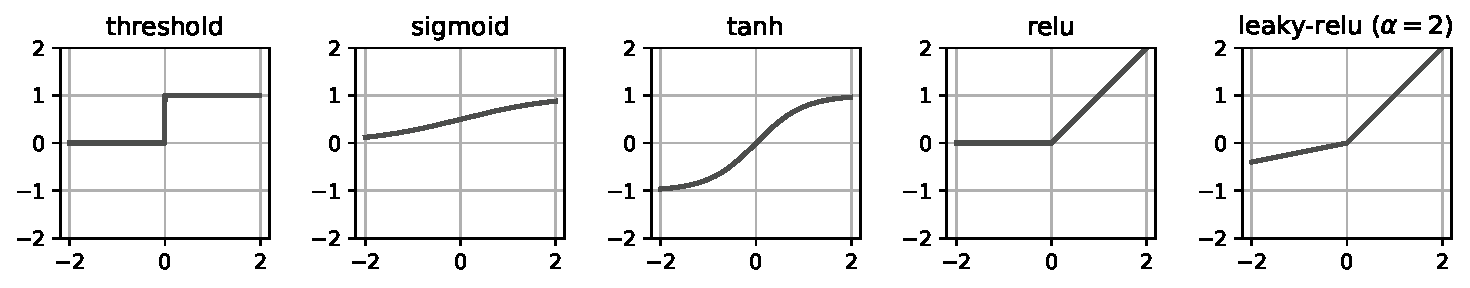
\includegraphics[width=1.0\linewidth]{./figures/neural_nets/pointwise_nonlinearities.pdf}
    }
    \caption{Common pointwise nonlinearities.}
    \label{fig:neural_nets:pointwise_nonlinearities}
\end{figure}

If a net only contained linear layers then it could only compute linear functions. This is because the composition of $N$ linear functions is a linear function. \index{Activation function}\textbf{Activation layers} add nonlinearity. Activation layers are typically pointwise functions, applying a scalar to scalar mapping on each dimension of the input vector. Typically parameters of these layers, if any, are not learned (but they can be). Some common activation layers are defined below and are plotted in \fig{\ref{fig:neural_nets:pointwise_nonlinearities}}:
\begin{align}
    \textcolor{data_color_dark}{\xoutindexed}[i] &= 
        \begin{cases}
            1, &\text{if} \quad \textcolor{data_color_dark}{\xinindexed}[i] > 0\\
            0,              & \text{otherwise}
        \end{cases} & \quad\quad \triangleleft \quad \texttt{threshold}\\
    \textcolor{data_color_dark}{\xoutindexed}[i] &= \frac{1}{1 + e^{-\textcolor{data_color_dark}{\xinindexed}[i]}} & \quad\quad \triangleleft \quad \texttt{sigmoid}\\
    \textcolor{data_color_dark}{\xoutindexed}[i] &= 2*\texttt{sigmoid}(2*\textcolor{data_color_dark}{\xinindexed}[i])-1 & \quad\quad \triangleleft \quad \texttt{tanh}\\
    \textcolor{data_color_dark}{\xoutindexed}[i] &= \max(\textcolor{data_color_dark}{\xinindexed}[i],0) & \quad\quad \triangleleft \quad \texttt{relu}\\
    \textcolor{data_color_dark}{\xoutindexed}[i] &= 
        \begin{cases}
            \max(\textcolor{data_color_dark}{\xinindexed}[i],0), &\text{if} \quad \textcolor{data_color_dark}{\xinindexed}[i] \geq 0\\
            \textcolor{param_color_dark}{a}\min(\textcolor{data_color_dark}{\xinindexed}[i],0),              & \text{otherwise}
        \end{cases} & \quad\quad \triangleleft \quad \texttt{leaky-relu}
\end{align}

\subsection{Normalization Layers}\label{sec:neural_nets:normalization_layers}
\index{Normalization layers}
Normalization layers add another kind of nonlinearity. Instead of being a pointwise nonlinearity, like in activation layers, they are nonlinearities that perturb each neuron based on the collective behavior of a set of neurons. Let's start with the example of \index{Batch normalization}{\bf batch normalization} (\textbf{batchnorm})~\cite{ioffe2015batch}.

Batchnorm {\bf standardizes} each neural activation with respect to its mean and variance over a batch of datapoints. Mathematically, 
\begin{align}
    \textcolor{data_color_dark}{\xoutindexed}[i] = \textcolor{param_color_dark}{\gamma}\frac{\textcolor{data_color_dark}{\xinindexed}[i] - \mathbb{E}[\textcolor{data_color_dark}{\xinindexed}[i]]}{\sqrt{\texttt{Var}[\textcolor{data_color_dark}{\xinindexed}[i]]}} + \textcolor{param_color_dark}{\beta} & \quad\quad \triangleleft \quad \texttt{batchnorm}
\end{align}
\marginnote{Recall from statistics that the standard score of a draw of a random variable is how many standard deviations it differs from the mean: $z = \frac{x-\mu}{\sigma}$.}[-0.4cm]
where $\textcolor{param_color_dark}{\gamma}$ and $\textcolor{param_color_dark}{\beta}$ are learned parameters of this layer that maintain expressivity so that the layer can output values with non-zero mean and non-unit variance. Most commonly batchnorm is applied using training batch statistics to compute the mean and variance, which change batch to batch. At test time, aggregate statistics from the training data are used. However, using test batch statistics can be useful for achieving invariance to changes in the statistics from training data to test data~\cite{wang2020fully}.

There are numerous other normalization layers that have been defined over the years. Two more that we will highlight are \index{$L_2$ normalization}\textbf{$L_2$ normalization} and \index{Layer normalization}\textbf{layer normalization} (\textbf{layernorm})~\cite{ba2016layer}. $L_2$ normalization projects the inputs onto the unit hypersphere, which useful for bounding the activations to unit vectors:
\begin{align}
    \textcolor{data_color_dark}{\xoutindexed}[i] &= \frac{\textcolor{data_color_dark}{\xinindexed}[i]}{\norm{\textcolor{data_color_dark}{\xin}}_2} & \quad\quad \triangleleft \quad \texttt{L2-norm}
\end{align}
%This operation projects the inputs onto the unit hypersphere -- quite a nice trick.
Layernorm is similar except that it standardizes the vector of input activations:
\begin{align}
    \mu &= \frac{1}{n} \sum_{i=1}^n \textcolor{data_color_dark}{\xinindexed}[i]\\
    \sigma^2 &= \frac{1}{n} \sum_{i=1}^n (\textcolor{data_color_dark}{\xinindexed}[i] - \mu)^2\\
    \textcolor{data_color_dark}{\xoutindexed}[i] &= \textcolor{param_color_dark}{\gamma}\frac{\textcolor{data_color_dark}{\xinindexed}[i] - \mu}{\sigma} + \textcolor{param_color_dark}{\beta} & \quad\quad \triangleleft \quad \texttt{layernorm}
\end{align}
\marginnote{Notice that layernorm, like $L_2$-normalization, maps the activation vector to the surface of a hypersphere, but it also centers the activations to have zero mean, and then scales and shifts the activations via $\gamma$ and $\beta$. As an exercise, see if you can write layernorm using $L_2$-normalization as one of the steps.}[-3.2cm]
Notice that layernorm also looks quite similar to batchnorm. Both standardize activations but do so with respect to different statistics. Layernorm computes a mean and variance over elements of a datapoint $\xin$, and will do so separately for each such datapoint in a batch. Batchnorm computes the mean and variance per channel over datapoints in a batch. If we have a batch stored in the tensor $\mathbf{X} \in \mathbb{R}^{N_{\texttt{batch}} \times C}$, then what layernorm does looks just like a ``transpose'' of what batchnorm does. Batchnorm standardizes each element of the tensor by the mean and variance of its column. Layernorm standardizes each element by the mean and variance of its row:
\begin{figure}[h!]
    \centerline{
    %\noindent\hspace{0.05\linewidth}
    %\begin{minipage}{0.65\linewidth}
    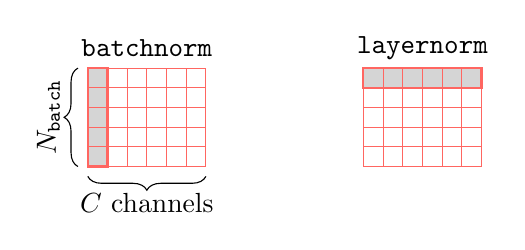
\begin{tikzpicture}
        \def\Nbatch{5}
        \def\Nchannels{6}
        \def\cellwidth{0.25}
        %
        % draw batchnorm
        \draw[step=\cellwidth,color=data_color_dark,fill=gray!33, thick] (0,0) rectangle ++(1*\cellwidth, -\Nbatch*\cellwidth);
        \draw[step=\cellwidth,color=data_color_dark] (0,0) grid (\Nchannels*\cellwidth, -\Nbatch*\cellwidth); 
        \node at (\Nchannels*0.5*\cellwidth, \cellwidth) {\texttt{batchnorm}};
        \draw [decorate,decoration={brace, amplitude=5pt, angle=0}] (\Nchannels*\cellwidth, -\Nbatch*\cellwidth-\cellwidth*0.5) -- (0, -\Nbatch*\cellwidth-\cellwidth*0.5);
        \draw (\Nchannels*0.5*\cellwidth, -\Nbatch*\cellwidth-1.85*\cellwidth) node {$C \text{ channels}$};
        \draw [decorate,decoration={brace, amplitude=5pt, angle=0}] (-\cellwidth*0.5, -\Nbatch*\cellwidth) -- (-\cellwidth*0.5, 0);
        \node [rotate=90] at (-\cellwidth*2, -\Nbatch*0.5*\cellwidth) {$N_{\texttt{batch}}$};
        %
        % draw layernorm
        \pgfmathsetmacro{\myshift}{\cellwidth*\Nchannels+2}
        \begin{scope}[xshift=\myshift cm]
            \draw[step=\cellwidth,color=data_color_dark,fill=gray!33, thick] (0,0) rectangle ++(\Nchannels*\cellwidth, -1*\cellwidth);
            \draw[step=\cellwidth,color=data_color_dark] (0,0) grid (\Nchannels*\cellwidth, -\Nbatch*\cellwidth);
            \node at (\Nchannels*0.5*\cellwidth, \cellwidth) {\texttt{layernorm}};
        \end{scope}
    \end{tikzpicture}
    %\end{minipage}
    }
    \caption{Batchnorm vs layernorm. Gray indicates the region over which mean and variance are computed. See also Figure 2 of \cite{wu2018group} for more such visualizations.}
    \label{fig:neural_nets:batchnorm_vs_layernorm_diagram}
\end{figure}

%\marginnote{See Figure 2 of \cite{wu2018group} for further normalization schemes visualized this way.}[-1cm]

One issue with batchnorm is that it requires processing a batch of datapoints all at once, and introduces a dependency between each datapoint in the batch. This violates the principle that datapoints should be processed independently and identically (iid), and this can lead to bugs if your method relies on the iid assumption. Layernorm does not have this problem and does indeed process each datapoint in an iid fashion.

\subsection{Output Layers}
The last piece we need is an \textbf{output layer} that maps a neural representation—a high-dimensional array of floating point numbers—to a desired output representation. In classification problems, the desired output is a class label, and the most common output operation is the softmax function, which we have already encountered in previous chapters. In image synthesis problems, the desired output is typically a 3D array with dimensions $N \times M \times 3$, and values in the range $[0,255]$. A sigmoid multiplied by 255 is a typical output transformation for this setting. The equations for these two layers are:
\begin{align}
    \textcolor{data_color_dark}{\xoutindexed}[i] &= \frac{e^{-\textcolor{param_color_dark}{\tau}\textcolor{data_color_dark}{\xinindexed}[i]}}{\sum_{k=1}^K e^{-\textcolor{param_color_dark}{\tau}\textcolor{data_color_dark}{\xinindexed}[k]}} & \quad\quad \triangleleft \quad \texttt{softmax}\\
    \textcolor{data_color_dark}{\xoutindexed}[i] &= 255*\texttt{sigmoid}(\textcolor{data_color_dark}{\xinindexed}[i]) & \quad\quad \triangleleft \quad \text{common layer for image output problems}
\end{align}
In the softmax definition we have added a {\bf temperature} parameter $\textcolor{param_color_dark}{\tau}$, which is used to scale how peaky, or confident, the predictions are.

The output layer is the input to the loss function, thus completing our specification of the deep learning problem. However, to use the outputs in practice requires translating them into actual pictures, or actions, or decisions. For a classification problem, this might mean taking the argmax of the softmax distribution, so that we can report a single class. For image prediction problems, it might mean rounding each output to an integral value since common image formats represent RGB values as integers.

There are of course many other output transformations you can try. Often, they will be very problem specific since they depend on the structure of the output space you are targeting.


\section{Why Are Neural Networks a Good Architecture?}
As you will soon learn, almost all modern computer vision algorithms involve deep nets in one way or another. So you may be wondering: why are deep nets such a good architecture? We will highlight here five reasons:
\begin{enumerate}
    \item They are high capacity (big enough nets are universal approximators).
    \item They are differentiable (the parameters can be optimized via gradient descent).
    \item They have good inductive biases (neural architectures reflect real structure in the world).
    \item They run efficiently on parallel hardware.
    \item They build abstractions.
\end{enumerate}
Let's look at reasons 1-3 in light of the discussion of searching for truth from \chap{\ref{chapter:problem_of_generalization}} (see \fig{\ref{fig:problem_of_generalization:search_space_tools}}). Reason 1 relates to the size of the hypothesis space. The hypothesis space can be made very big if we use a large neural network with many parameters. So we can usually be sure that our true solution (or a close approximation to it) does indeed lie in the space spanned by the neural net architecture. Reason 2 says that searching for the solution within this space is relatively easy, since we can use gradients to direct us toward ever better fits to the data. Reason 3 is one we will only come to appreciate later in the book as we investigate more advanced neural net architectures. It turns out that these architectures impose constraints and regularizers that bias our search toward solutions that capture true structure about the visual world, and this leads to learned solutions that generalize.

Reason 4 is equally important to the first three: it says we can do all of this \textit{efficiently} because most computations can be parallelized on modern hardware; in particular both matrix multiplies (linear layers) and pointwise operations (e.g., relu layers) are easy to parallelize on graphical processing units. Further, most operations are applied to image batches, where each item in the batch can be sent to a different parallel compute node.

Reason 5 is the perhaps the most subtle. It is related to the layered structure of neural nets. Layer by layer, neural nets build up increasingly abstracted representations of the input data, and these abstractions tend to be increasingly useful. This argument is not easy to appreciate at first glance, but it will be a major theme of the subsequent chapters in this book, especially those on representation learning. For now, just keep in mind that the \textit{internal representations} that are built up layer by layer in deep nets are useful and important beyond just the net's overall input-output behavior.


%and \#5 are the most subtle one, and they are the major focus of the field of neural network architecture design. In fact, the first three reasons are in a sense not so special: there are innumerable simple learning machines that all have properties 1 through 3. For example, a (distributed) lookup table has properties \#1 and \#3 and does not need property \#2 since learning is trivial (just add a row to the table for each new training point observed). What is special about neural nets is more in properties \#4 and \#5: why their architecture supports fast inference and finds solutions that generalize.


% \subsection{Depth vs width: deep nets can require fewer parameters than wide nets}
% \reviewcomment{Unfinished}

% A rule of thumb in deep learning is that bigger networks perform better. But networks can be bigger in several different ways: they can be \textit{deep} and/or they can be \textit{wide}. The \textbf{depth} of a network is its number of layers. The \textbf{width} of a network is the number of neurons on each layer (if different layers have different numbers of neurons then we may specify the width per layer). 

% Is it better to make a network deeper or wider? Universal approximation theory tells us that a sufficiently wide network can fit any function. If you are underfitting, you can add more width to increase your networks capacity and potentially fit better.

% Increasing network depth also increases its capacity, but not in quite the same way. Interestingly, it is sometimes the case that deep nets require far fewer parameters to fit data than wide nets. Evidence for this statement comes mostly from empirical practice, where researchers have found that deep nets just work better on many popular problems. 

% However, there is also the beginning of a mathematical theory of when and why this can happen. The basic idea of this theory is to establish that there are certain classes of function that can be represented with a polynomial number of neurons in a depth $d$ network but require an exponential number of neurons in a depth $d^\prime$ network, for certain $d^\prime < d$. Arguments along these lines are called \textbf{depth separations}, and the interested reader can refer to \cite{telgarsky2016benefits} to learn more about this ongoing line of research.

% %There is also the beginning of theoretical evidence for why this is the case, but this area of research is still in its infancy.

% \subsection{Deep nets are biased to find simple solutions}
% \reviewcomment{Unfinished}
% For many years, it was thought that large neural nets had far too many degrees of freedom and therefore would overfit the data they were trained one. Recall from Chapter \ref{chapter:problem_of_generalization} that the more degrees of freedom a model has (the larger its hypothesis space), the more it spurious solutions exist that fit the data but are far from the true data-generating process. However, it has by now become clear that in practice deep nets usually do \textit{not} overfit, and instead generalize remarkably well.

% Why don't deep nets overfit? An emerging explanation is that \textit{deeper nets learn simpler functions}~\cite{valle-perez, huh}. 


\section{Concluding Remarks}
Neural nets are a very simple and useful parameterized hypothesis space. They are universal approximators that can be trained via gradient descent and run on parallel hardware. \textit{Deep} nets are especially effective in computer vision; as we will soon see, deep architectures can be constructed that specifically reflect structure in the visual world, making visual processing highly efficient and performant. Artificial neural nets also have connections to the real neural nets in our brains. This connection runs deeper than merely sharing a name: the deep net architectures we will see later in this book (e.g., convolutional networks, transformers) are our best current models of computation in animal brains, in the sense that they explain brain data better than any competing models~\cite{Schrimpf2020integrative}. This is a class of models truly worth paying attention to. %Remarkably, both evolution and engineering have both arrived at a similar architecture for visual intelligence. % PHILLIP
% 
%\setcounter{chapter}{12}
\chapter{Neural Networks as Distribution Transformers}\label{chapter:neural_nets_as_distribution_transformers}

\pgfplotsset{
    compat=1.3,
    rep2rep axis style/.style={
            width=1.0\textwidth,
            height=1.0\textwidth,
            axis lines=bottom,
            axis line style={stealth-stealth},
            y axis line style={draw=none},
            ymajorticks=false,
            xtick distance=0.5,
            tick style={draw=none},
            xmin=0,xmax=1,
            ymin=0,ymax=1,
        },
}

\section{Introduction}
So far we have seen that deep nets are stacks of simple functions, which compose to achieve interesting mappings from inputs to outputs. This section will introduce a slightly different way of thinking about deep nets. The idea is think of each layer as a \emph{geometric transformation of a data distribution}.

\section{A Different Way of Plotting Functions}
Each layer in a deep net is a mapping from one representation of the data to another: $f: \xin \rightarrow \xout$. If $\xin$ and $\xout$ are both one-dimensional (1D), then we can plot the mapping as a function with $\xin$ on the $x$-axis and $\xout$ on the $y$-axis (\fig{\ref{fig:neural_nets_as_distribution_transformers:trad_plot}}):

%\vspace{-0.5cm}
\begin{figure}[h]
\centerline{
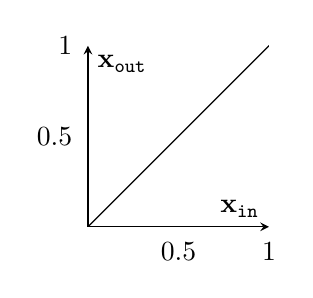
\begin{tikzpicture}
    \begin{axis}[
            width=0.32\textwidth,
            height=0.32\textwidth,
            xlabel={$\xin$},
            ylabel={$\xout$},
            axis lines=center,
            xtick distance=0.5,
            ytick distance=0.5,
            tick style={draw=none},
            xmin=0,xmax=1,
            ymin=0,ymax=1
    ]
    
    \addplot +[mark=none,smooth,black] {x};
    
    \end{axis}
\end{tikzpicture}
}
\caption{The traditional way of plotting the function $\xout = \xin$.}
\label{fig:neural_nets_as_distribution_transformers:trad_plot}
%\vspace{-0.5cm}
\end{figure}

Now, we will instead consider a different way of plotting the mapping, where we simply rotate the $y$-axis to be horizontal rather than vertical (\fig{\ref{fig:neural_nets_as_distribution_transformers:new_way_plot}}):

%\vspace{-0.5cm}
\begin{figure}[h]
\centering
\begin{minipage}[t][4.5cm][c]{0.32\textwidth}
\begin{tikzpicture}
    \begin{axis}[
            width=1.0\textwidth,
            height=1.0\textwidth,
            xlabel={$\xin$},
            ylabel={$\xout$},
            axis lines=center,
            tick style={draw=none},
            xtick distance=0.5,
            ytick distance=0.5,
            xmin=0,xmax=1,
            ymin=0,ymax=1,
    ]
    
    \addplot +[mark=none,smooth,black] {x};
    
    \addplot[scatter src=explicit symbolic, only marks, mark=triangle*, mark options={rotate=90}] coordinates {
        (0.03,0.1)
        (0.03,0.2)
        (0.03,0.3)
        (0.03,0.4)
        (0.03,0.5)
        (0.03,0.6)
        (0.03,0.7)
        (0.03,0.8)
    };
    
    \addplot[scatter src=explicit symbolic, only marks, mark=*] coordinates {
        (0.1,0)
        (0.2,0)
        (0.3,0)
        (0.4,0)
        (0.5,0)
        (0.6,0)
        (0.7,0)
        (0.8,0)
    };
    
    \addplot[mark=none,dashed] coordinates {
    	(0.1,0)
    	(0.1,0.1)
    };
    \addplot[mark=none,dashed] coordinates {
    	(0.2,0)
    	(0.2,0.2)
    };
    \addplot[mark=none,dashed] coordinates {
    	(0.3,0)
    	(0.3,0.3)
    };
    \addplot[mark=none,dashed] coordinates {
    	(0.4,0)
    	(0.4,0.4)
    };
    \addplot[mark=none,dashed] coordinates {
    	(0.5,0)
    	(0.5,0.5)
    };
    \addplot[mark=none,dashed] coordinates {
    	(0.6,0)
    	(0.6,0.6)
    };
    \addplot[mark=none,dashed] coordinates {
    	(0.7,0)
    	(0.7,0.7)
    };
    \addplot[mark=none,dashed] coordinates {
    	(0.8,0)
    	(0.8,0.8)
    };
    
    \addplot[mark=none,dashed] coordinates {
    	(0,0.1)
    	(0.1,0.1)
    };
    \addplot[mark=none,dashed] coordinates {
    	(0,0.2)
    	(0.2,0.2)
    };
    \addplot[mark=none,dashed] coordinates {
    	(0,0.3)
    	(0.3,0.3)
    };
    \addplot[mark=none,dashed] coordinates {
    	(0,0.4)
    	(0.4,0.4)
    };
    \addplot[mark=none,dashed] coordinates {
    	(0,0.5)
    	(0.5,0.5)
    };
    \addplot[mark=none,dashed] coordinates {
    	(0,0.6)
    	(0.6,0.6)
    };
    \addplot[mark=none,dashed] coordinates {
    	(0,0.7)
    	(0.7,0.7)
    };
    \addplot[mark=none,dashed] coordinates {
    	(0,0.8)
    	(0.8,0.8)
    };
    
\end{axis}
\end{tikzpicture}
\end{minipage}
\begin{minipage}[t][4.5cm][c]{0.1\textwidth}
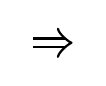
\begin{tikzpicture}
    \draw [line width=1pt, double distance=2pt, -{Classical TikZ Rightarrow[length=2mm]}] (0,0) -- (0.5,0);
\end{tikzpicture}
\end{minipage}
\begin{minipage}[t][4.5cm][c]{0.32\textwidth}
\begin{tikzpicture}
    
    % \begin{axis}[
    %         rep2rep axis style,
    %         xlabel={$\xin$},
    %         ylabel={$\xout$},
    %         axis x line=bottom, % Place the x-axis on the bottom
    %         axis y line=top,    % Place the y-axis on the top
    % ]

    \begin{axis}[
            rep2rep axis style,
            xlabel={$\xin$},
    ]
    \end{axis}
    
    \begin{axis}[
            rep2rep axis style,
            xlabel={$\xout$},
            axis lines=top,
    ]
    
    \addplot[mark=none,dashed] coordinates {
    	(0.1,0)
    	(0.1,1)
    };
    \addplot[mark=none,dashed] coordinates {
    	(0.2,0)
    	(0.2,1)
    };
    \addplot[mark=none,dashed] coordinates {
    	(0.3,0)
    	(0.3,1)
    };
    \addplot[mark=none,dashed] coordinates {
    	(0.4,0)
    	(0.4,1)
    };
    \addplot[mark=none,dashed] coordinates {
    	(0.5,0)
    	(0.5,1)
    };
    \addplot[mark=none,dashed] coordinates {
    	(0.6,0)
    	(0.6,1)
    };
    \addplot[mark=none,dashed] coordinates {
    	(0.7,0)
    	(0.7,1)
    };
    \addplot[mark=none,dashed] coordinates {
    	(0.8,0)
    	(0.8,1)
    };
    \addplot[mark=none,dashed] coordinates {
    	(0.9,0)
    	(0.9,1)
    };
    
    \addplot[scatter src=explicit symbolic, only marks, mark=*] coordinates {
        (0.1,0)
        (0.2,0)
        (0.3,0)
        (0.4,0)
        (0.5,0)
        (0.6,0)
        (0.7,0)
        (0.8,0)
        (0.9,0)
    };
    
    \addplot[scatter src=explicit symbolic, only marks, mark=triangle*] coordinates {
        (0.1,0.97)
        (0.2,0.97)
        (0.3,0.97)
        (0.4,0.97)
        (0.5,0.97)
        (0.6,0.97)
        (0.7,0.97)
        (0.8,0.97)
        (0.9,0.97)
    };
    
\end{axis}
\end{tikzpicture}
\end{minipage}
\caption{An alternative way of plotting a function (right). Functions are mappings that rearrange the input space. The identity function $\xout=\xin$, shown here, means ``no rearrangement,'' so the mapping is straight lines.}
\label{fig:neural_nets_as_distribution_transformers:new_way_plot}
%\vspace{-0.5cm}
\end{figure}

The depiction to the right makes it obvious that the plot $\xout = \xin$ is the identity mapping: datapoints get mapped to unchanged positions. \Fig{\ref{fig:neural_nets_as_distribution_transformers:new_way_plot_examples}} shows a few more mappings plotted in this way:
\begin{figure}[h]
\begin{minipage}[t][5.0cm][c]{0.45\textwidth}
%\begin{minipage}[t][5.5cm][c]{0.45\textwidth}
%\begin{flushleft}
\begin{tikzpicture}
    \begin{axis}[
            rep2rep axis style,
            width=0.78\textwidth,
            height=0.6\textwidth,
            title={$\xout = 2\xin$},
            title style={at={(0.1,0.5)},anchor=north east,draw=black,fill=white},
            xlabel={$\xin$},
            xmin=-1.2,xmax=1.2,
    ]
    \end{axis}
    
    \begin{axis}[
            rep2rep axis style,
            width=0.78\textwidth,
            height=0.6\textwidth,
            xlabel={$\xout$},
            axis lines=top,
            xmin=-1.2,xmax=1.2,
    ]
    
    \addplot[mark=none,dashed] coordinates {
    	(-0.5,0)
    	(-1.0,1)
    };
    \addplot[mark=none,dashed] coordinates {
    	(-0.25,0)
    	(-0.5,1)
    };
    \addplot[mark=none,dashed] coordinates {
    	(0,0)
    	(0,1)
    };
    \addplot[mark=none,dashed] coordinates {
    	(0.25,0)
    	(0.5,1)
    };
    \addplot[mark=none,dashed] coordinates {
    	(0.5,0)
    	(1,1)
    };
    
    \addplot[scatter src=explicit symbolic, only marks, mark=*] coordinates {
        (-0.5,0)
        (-0.25,0)
        (0,0)
        (0.25,0)
        (0.5,0)
    };
    
    \addplot[scatter src=explicit symbolic, only marks, mark=triangle*] coordinates {
        (-1,0.97)
        (-0.5,0.97)
        (0,0.97)
        (0.5,0.97)
        (1,0.97)
    };
\end{axis}
\end{tikzpicture}
%\end{flushleft}
\end{minipage}
\begin{minipage}[t][5.0cm][c]{0.45\textwidth}
%\begin{minipage}[t][5.5cm][c]{0.45\textwidth}
%\begin{flushright}
\begin{tikzpicture}
    \begin{axis}[
            rep2rep axis style,
            width=0.78\textwidth,
            height=0.6\textwidth,
            title={$\xout = \frac{\xin + 1}{2}$},
            title style={at={(0.1,0.5)},anchor=north east,draw=black,fill=white},
            xlabel={$\xin$},
            xmin=-1.2,xmax=1.2,
    ]
    \end{axis}
    
    \begin{axis}[
            rep2rep axis style,
            width=0.78\textwidth,
            height=0.6\textwidth,
            xlabel={$\xout$},
            axis lines=top,
            xmin=-1.2,xmax=1.2,
    ]
    
    \addplot[mark=none,dashed] coordinates {
    	(-1.0,0)
    	(0,1)
    };
    \addplot[mark=none,dashed] coordinates {
    	(-0.5,0)
    	(0.25,1)
    };
    \addplot[mark=none,dashed] coordinates {
    	(0,0)
    	(0.5,1)
    };
    \addplot[mark=none,dashed] coordinates {
    	(0.5,0)
    	(0.75,1)
    };
    \addplot[mark=none,dashed] coordinates {
    	(1,0)
    	(1,1)
    };
    
    \addplot[scatter src=explicit symbolic, only marks, mark=*] coordinates {
        (-1,0)
        (-0.5,0)
        (0,0)
        (0.5,0)
        (1,0)
    };
    
    \addplot[scatter src=explicit symbolic, only marks, mark=triangle*] coordinates {
        (0,0.97)
        (0.25,0.97)
        (0.5,0.97)
        (0.75,0.97)
        (1,0.97)
    };
\end{axis}
\end{tikzpicture}
%\end{flushright}
\end{minipage}
\begin{minipage}[t][5.0cm][c]{0.45\textwidth}
%\begin{flushleft}
\begin{tikzpicture}
    \begin{axis}[
            rep2rep axis style,
            width=0.78\textwidth,
            height=0.6\textwidth,
            title={$\xout = \texttt{relu}(\xin)$},
            title style={at={(0.1,0.5)},anchor=north east,draw=black,fill=white},
            xlabel={$\xin$},
            xmin=-1.2,xmax=1.2,
    ]
    \end{axis}
    
    \begin{axis}[
            rep2rep axis style,
            width=0.78\textwidth,
            height=0.6\textwidth,
            xlabel={$\xout$},
            axis lines=top,
            xmin=-1.2,xmax=1.2,
    ]
    
    \addplot[mark=none,dashed] coordinates {
    	(-1,0)
    	(0,1)
    };
    \addplot[mark=none,dashed] coordinates {
    	(-0.5,0)
    	(0,1)
    };
    \addplot[mark=none,dashed] coordinates {
    	(0,0)
    	(0,1)
    };
    \addplot[mark=none,dashed] coordinates {
    	(0.5,0)
    	(0.5,1)
    };
    \addplot[mark=none,dashed] coordinates {
    	(1,0)
    	(1,1)
    };
    
    \addplot[scatter src=explicit symbolic, only marks, mark=*] coordinates {
        (-1,0)
        (-0.5,0)
        (0,0)
        (0.5,0)
        (1,0)
    };
    
    \addplot[scatter src=explicit symbolic, only marks, mark=triangle*] coordinates {
        (0,0.97)
        (0.5,0.97)
        (0,0.97)
        (0.5,0.97)
        (1, 0.97)
    };
\end{axis}
\end{tikzpicture}
%\end{flushleft}
\end{minipage}
\begin{minipage}[t][5.0cm][c]{0.45\textwidth}
%\begin{flushright}
\begin{tikzpicture}
    \begin{axis}[
            rep2rep axis style,
            width=0.78\textwidth,
            height=0.6\textwidth,
            title={$\xout = \texttt{sigmoid}(\xin)$},
            title style={at={(0.1,0.5)},anchor=north east,draw=black,fill=white},
            xlabel={$\xin$},
            xmin=-5.2,xmax=5.2,
            xtick distance=2.5,
    ]
    \end{axis}
    
    \begin{axis}[
            rep2rep axis style,
            width=0.78\textwidth,
            height=0.6\textwidth,
            xlabel={$\xout$},
            axis lines=top,
            xmin=-1.2,xmax=1.2,
    ]
    
    \addplot[mark=none,dashed] coordinates {
    	(-1.0,0)
    	(0.007,1)
    };
    \addplot[mark=none,dashed] coordinates {
    	(-0.5,0)
    	(0.076,1)
    };
    \addplot[mark=none,dashed] coordinates {
    	(0,0)
    	(0.5,1)
    };
    \addplot[mark=none,dashed] coordinates {
    	(0.5,0)
    	(0.924,1)
    };
    \addplot[mark=none,dashed] coordinates {
    	(1,0)
    	(0.993,1)
    };
    
    \addplot[scatter src=explicit symbolic, only marks, mark=*] coordinates {
        (-1,0)
        (-0.5,0)
        (0,0)
        (0.5,0)
        (1,0)
    };
    
    \addplot[scatter src=explicit symbolic, only marks, mark=triangle*] coordinates {
        (0.007,0.97)
        (0.076,0.97)
        (0.5,0.97)
        (0.924,0.97)
        (0.993,0.97)
    };
    
\end{axis}
\end{tikzpicture}
%\end{flushright}
\end{minipage}
\caption{Mapping plots for several simple functions that could be neural layers.}
\label{fig:neural_nets_as_distribution_transformers:new_way_plot_examples}
\end{figure}

Each of the above are layers that could be found in a deep net. Linear layers, like those in the top row above, stretch and squash the data distribution. The relu nonlinearity maps all negative data to 0, and applies an identity map to all nonnegative data. The sigmoid function pulls negative data to 0 and positive data to 1.

\section{How Deep Nets Remap a Data Distribution}
In this way, an incoming data distribution can be reshaped layer by layer into a desired configuration. The goal of a binary softmax classifier, for example, is to move the datapoints around until all the class 0 points end up moved to $[1,0]$ on the output layer and all the class 1 points end up moved to $[0,1]$.
\marginnote{This is because the one-hot code for the integer 0 is $[1,0]$ and the one-hot code for the integer 1 is $[0,1]$.}[-1cm]

A deep net stacks these operations; an example is given in \fig{\ref{fig:neural_nets_as_distribution_transformers:new_way_plot_two_layer}}.
\begin{figure}[h]
%\noindent\hspace{0.25\linewidth}
\centerline{
\begin{tikzpicture}
    \begin{axis}[
            rep2rep axis style,
            width=0.35\textwidth,
            height=0.4\textwidth,
            title={$\mathbf{x}_1 = 2*\mathbf{x}_0$},
            title style={at={(0.1,0.25)},anchor=north east,draw=black,fill=white},
            xlabel={$\mathbf{x}_0$},
            xmin=-1.2,xmax=1.2,
    ]
    \end{axis}
    
    % \begin{axis}[
    %         rep2rep axis style,
    %         width=0.35\textwidth,
    %         height=0.25\textwidth,
    %         title={$\mathbf{x}^{(2)} = \texttt{relu}(\mathbf{x}^{(1)})$},
    %         title style={at={(0.1,1.5)},anchor=north east,draw=black,fill=white},
    %         xlabel={$\mathbf{x}^{(1)}$},
    %         axis lines=top,
    %         xmin=-1.2,xmax=1.2,
    % ]
    % \end{axis}
    
    \begin{axis}[
            rep2rep axis style,
            width=0.35\textwidth,
            height=0.4\textwidth,
            title={$\mathbf{x}_2 = \texttt{relu}(\mathbf{x}_1$},
             title style={at={(0.1,0.75)},anchor=north east,draw=black,fill=white},
            xlabel={$\mathbf{x}_2$},
            axis lines=top,
            xmin=-1.2,xmax=1.2,
            ymin=0,ymax=2
    ]
    
    \addplot[mark=none] coordinates {
    	(-1.2,1)
    	(1.2,1)
    };
    
    \addplot[mark=none,dashed] coordinates {
    	(-0.5,0)
    	(-1.0,1)
    };
    \addplot[mark=none,dashed] coordinates {
    	(-0.25,0)
    	(-0.5,1)
    };
    \addplot[mark=none,dashed] coordinates {
    	(0,0)
    	(0,1)
    };
    \addplot[mark=none,dashed] coordinates {
    	(0.25,0)
    	(0.5,1)
    };
    \addplot[mark=none,dashed] coordinates {
    	(0.5,0)
    	(1,1)
    };
    
    \addplot[scatter src=explicit symbolic, only marks, mark=*] coordinates {
        (-0.5,0)
        (-0.25,0)
        (0,0)
        (0.25,0)
        (0.5,0)
    };
    
    \addplot[scatter src=explicit symbolic, only marks, mark=triangle*] coordinates {
        (-1,0.97)
        (-0.5,0.97)
        (0,0.97)
        (0.5,0.97)
        (1,0.97)
    };
    
    \addplot[mark=none,dashed] coordinates {
    	(-1,1)
    	(0,2)
    };
    \addplot[mark=none,dashed] coordinates {
    	(-0.5,1)
    	(0,2)
    };
    \addplot[mark=none,dashed] coordinates {
    	(0,1)
    	(0,2)
    };
    \addplot[mark=none,dashed] coordinates {
    	(0.5,1)
    	(0.5,2)
    };
    \addplot[mark=none,dashed] coordinates {
    	(1,1)
    	(1,2)
    };
    
    \addplot[scatter src=explicit symbolic, only marks, mark=triangle*] coordinates {
        (0,1.97)
        (0,1.97)
        (0,1.97)
        (0.5,1.97)
        (1,1.97)
    };
    
\end{axis}

\end{tikzpicture}
}
\caption{Mapping plot for a \texttt{linear}-\texttt{relu} stack.}
\label{fig:neural_nets_as_distribution_transformers:new_way_plot_two_layer}
\end{figure}

The plots above show how a uniform grid of datapoints get mapped from layer to layer in a deep net. We can also use this plotting style to show how a nonuniform distribution of incoming datapoints gets transformed. This is the setting in which deep nets actually operate, and sometimes the real action of the network looks very different when viewed this way. We can think of a deep net as transforming an input data distribution, $\pdata$, into an output data distribution, $\pout$. Each layer of activations in a network is a different representation or \index{Embedding}{\bf embedding} of the data, and we can consider the distribution of activations on some layer $\ell$ to be $p_{\ell}$. Then, layer by layer, a deep net transforms $\pdata$ into $p_{\texttt{1}}$ into $p_{\texttt{2}}$, and so on until finally transforming the data to the distribution $\pout$. Most loss functions can also be interpreted from this angle: they penalize the divergence, in one form or another, between the output distribution $\pout$ and a target distribution $p_{\texttt{target}}$.

A nice property of this way of plotting is that it also extends to visualizing two-dimensional (2D)-to-2D mappings (something that conventional $x$-axis/$y$-axis plotting is not well equipped to do). Real deep nets perform $N$-dimensional (ND)-to-ND mappings, but already 2D-to-2D visualizations can give a lot of insight into the general case. In \fig{\ref{fig:neural_nets_as_data_transformations:2D_mapping_diagrams}}, we show how three common neural net layers may act to transform a Gaussian blob of data centered at the origin.
\begin{figure}[h]
\centerline{
\begin{minipage}{0.36\textwidth}
\begin{tikzpicture}
    \draw (0, 0) node[inner sep=0] {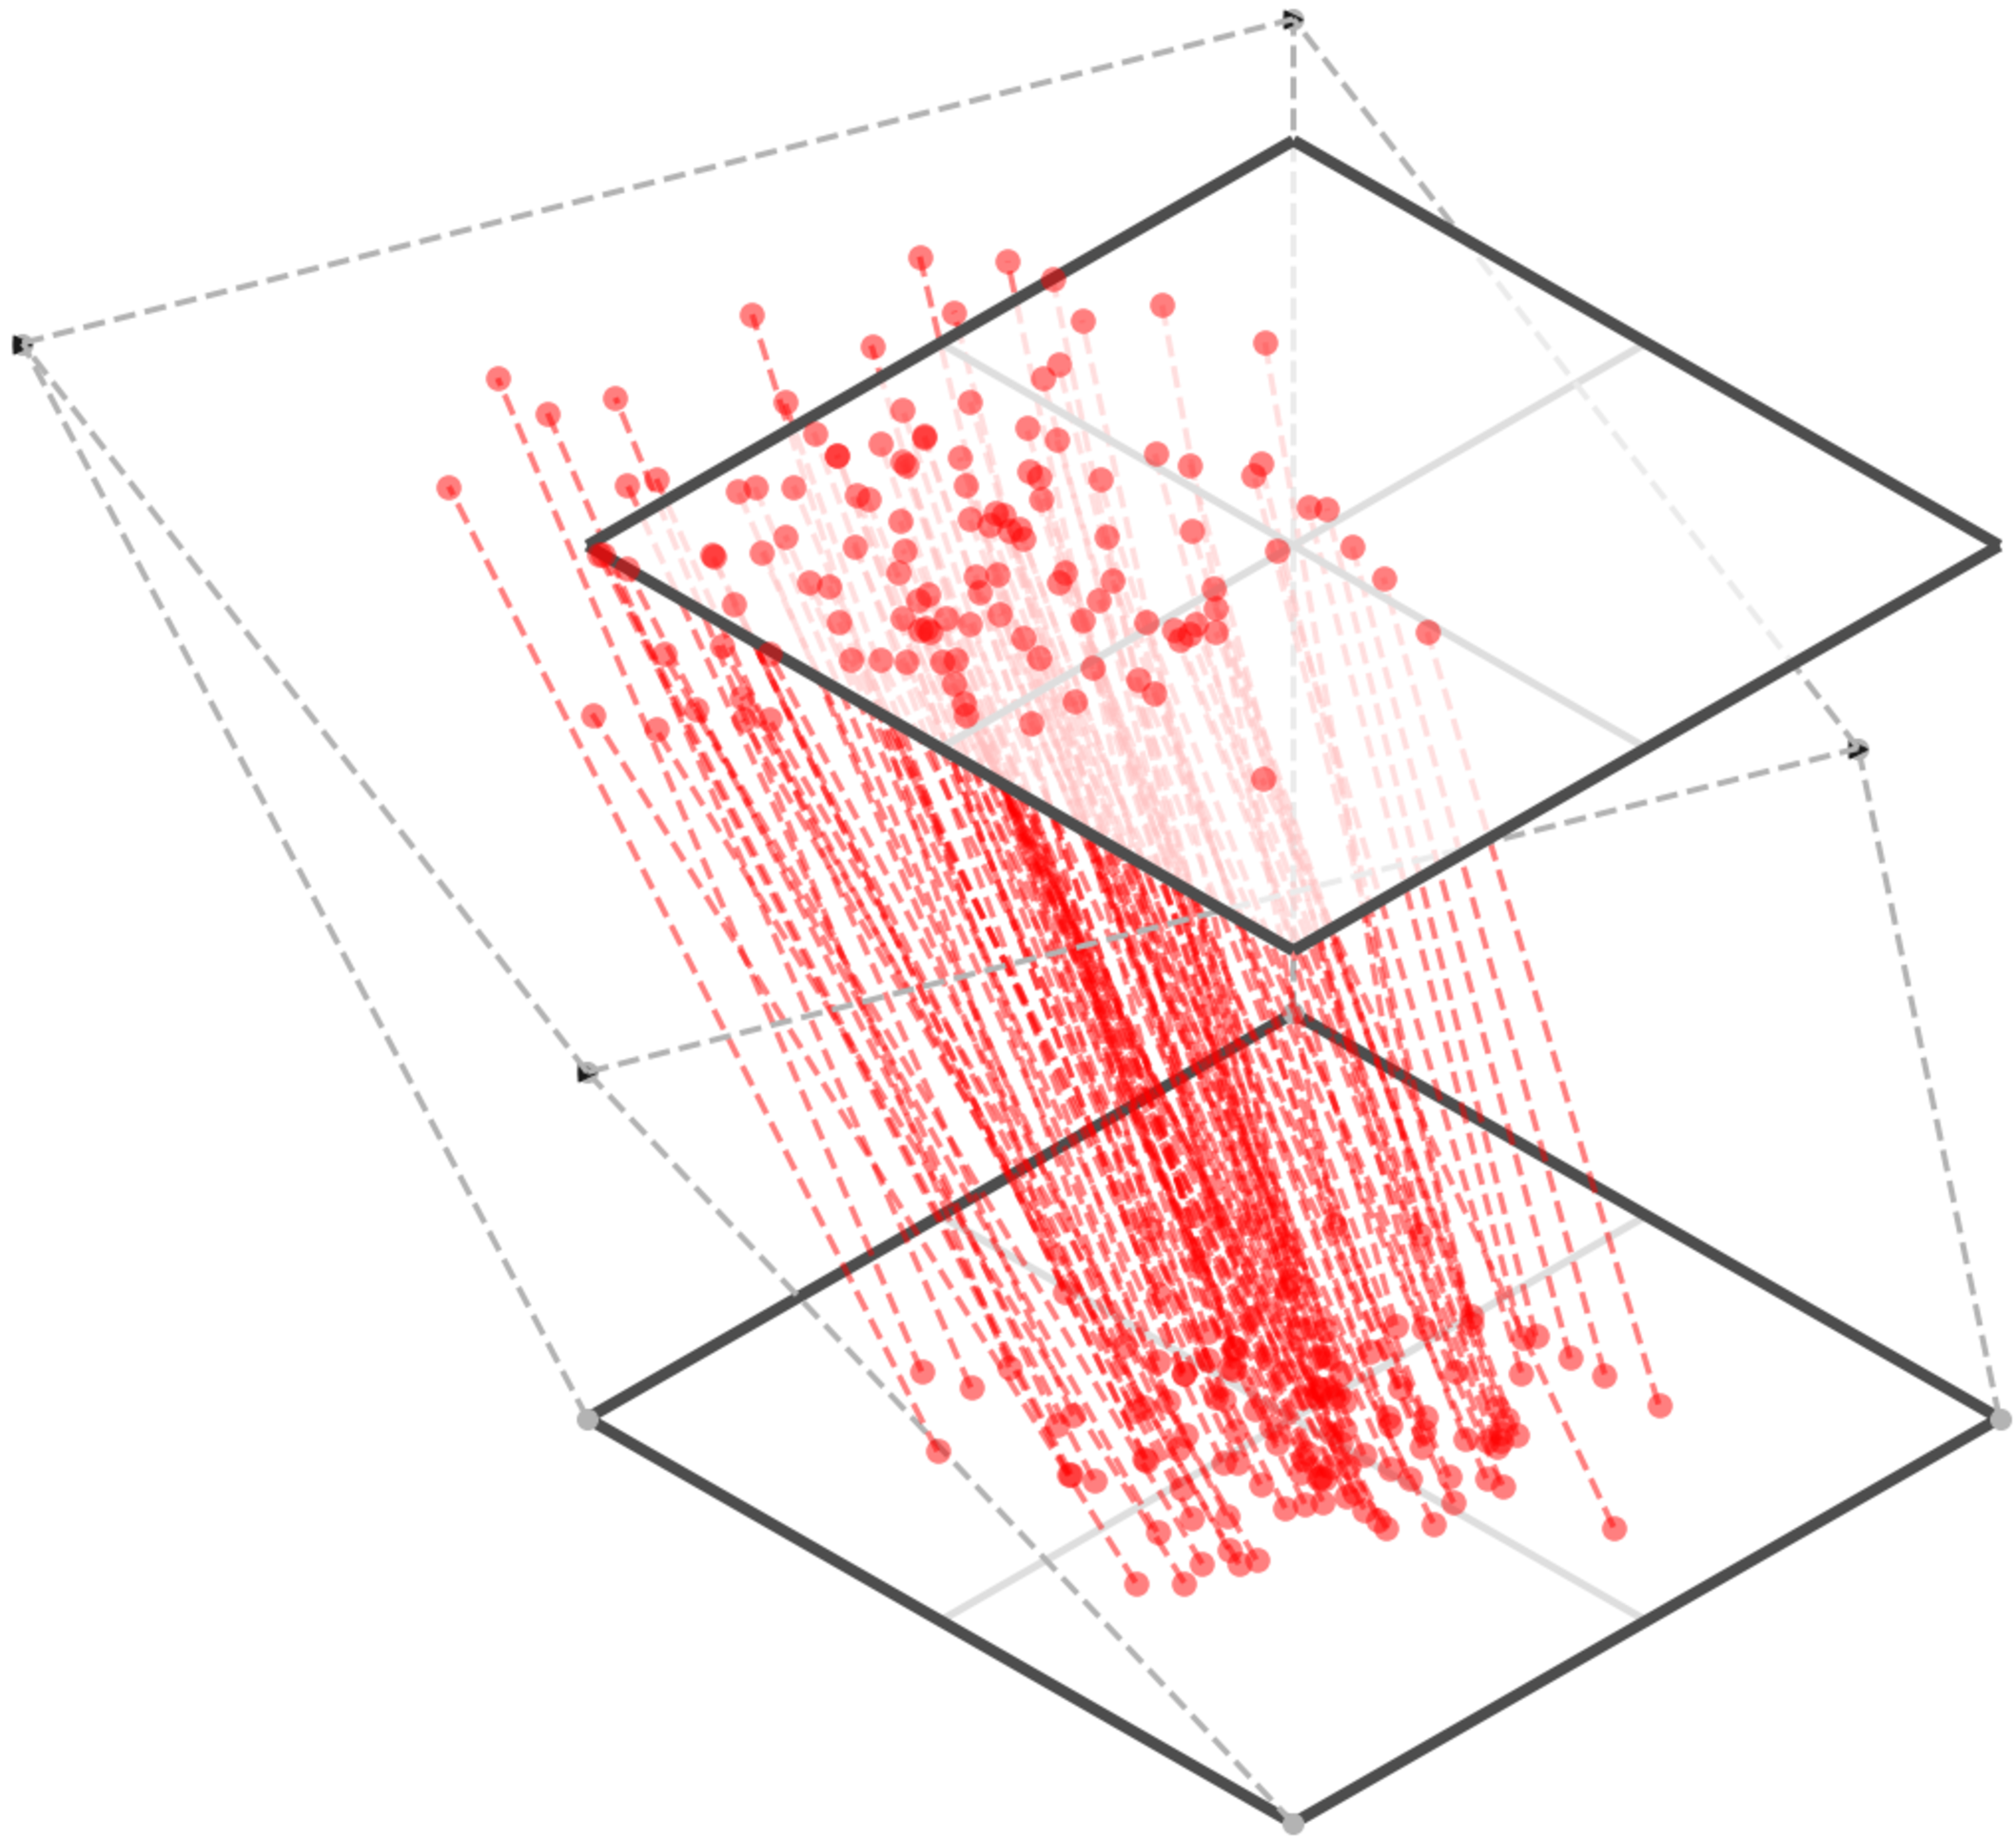
\includegraphics[width=0.8\linewidth]{figures/neural_nets/linear_layer_mapviz.pdf}};
    \draw (-1, -1.4) node {$\xin$};
    \draw (-1, 1.45) node {$\xout$};
    \draw (0, 2.3) node {\texttt{linear}};
\end{tikzpicture}
\end{minipage}
\begin{minipage}{0.28\textwidth}
\begin{tikzpicture}
    \draw (0, 0) node[inner sep=0] {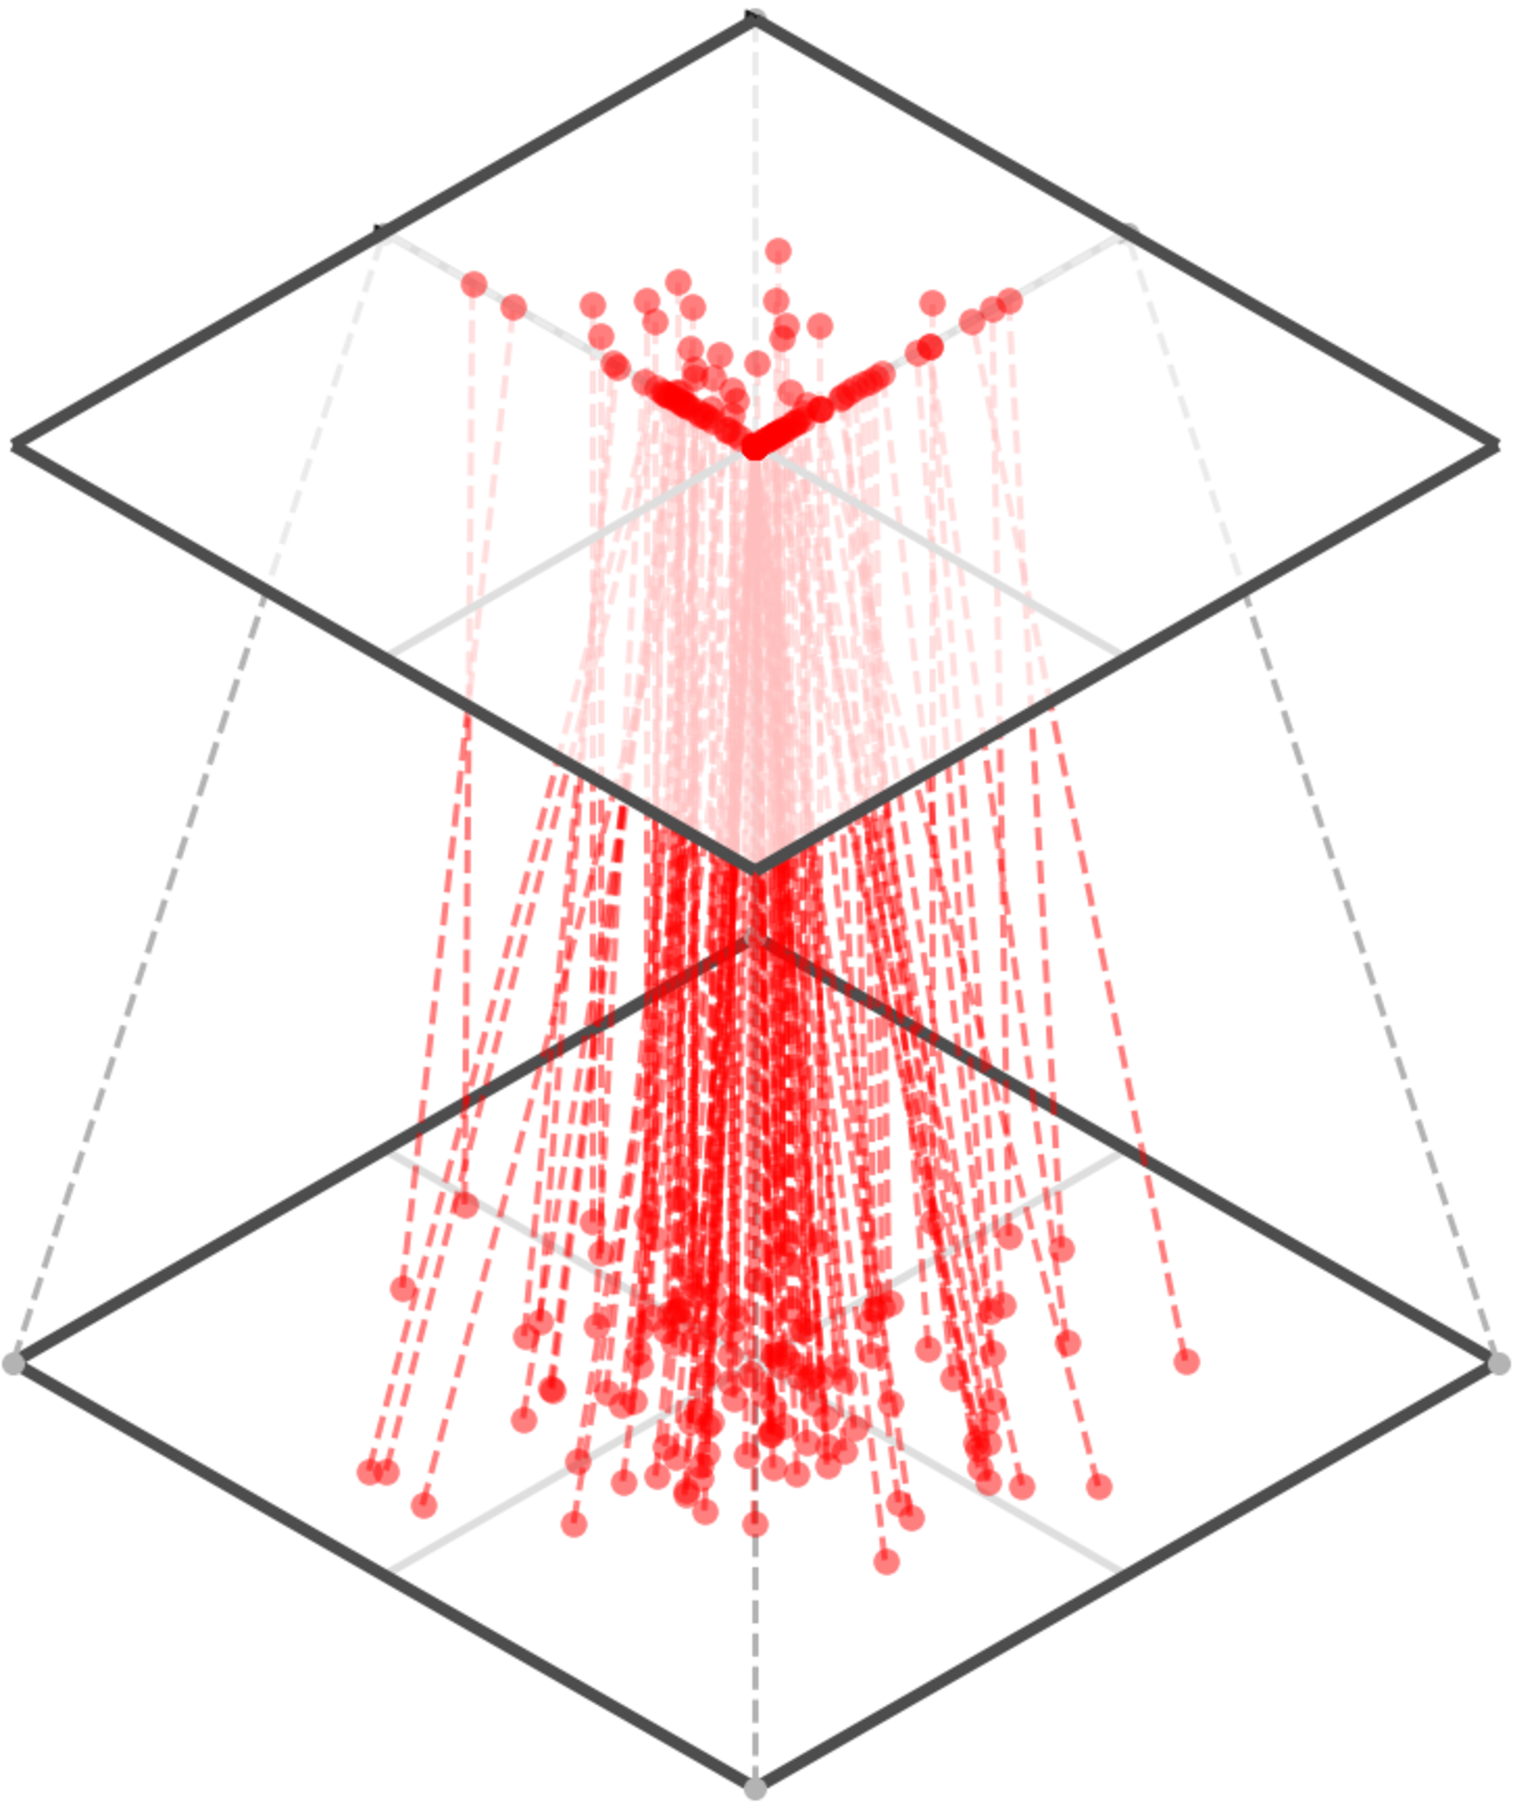
\includegraphics[width=0.8\linewidth]{figures/neural_nets/relu_layer_mapviz.pdf}};
    \draw (-1.6, -1.4) node {$\xin$};
    \draw (-1.6, 1.45) node {$\xout$};
    \draw (0, 2.3) node {\texttt{relu}};
\end{tikzpicture}
\end{minipage}
\begin{minipage}{0.28\textwidth}
\begin{tikzpicture}
    \draw (0, 0) node[inner sep=0] {\includegraphics[width=0.8\linewidth]{figures/neural_nets/L2norm_layer_mapviz.pdf}};
    \draw (-1.6, -1.4) node {$\xin$};
    \draw (-1.6, 1.45) node {$\xout$};
    \draw (0, 2.3) node {\texttt{L2-norm}};
\end{tikzpicture}
\end{minipage}
% \begin{minipage}{0.33\textwidth}
% \begin{flushright}
% \begin{tikzpicture}
%     \draw (0, 0) node[inner sep=0] {\includegraphics[width=1.0\linewidth]{figures/neural_nets/softmax_layer_mapviz.pdf}};
% \end{tikzpicture}
% \end{flushright}
% \end{minipage}
}
\caption{2D mapping diagrams for several neural layers. The \texttt{linear} layer mapping will shift, stretch, and rotate depending on its weights and biases.}
\label{fig:neural_nets_as_data_transformations:2D_mapping_diagrams}
\end{figure}


%Here is a linear layer $f: \mathbb{R}^2 \rightarrow \mathbb{R}^2$:
% Here are the linear and relu layers plotted this way, alongside other ways of representing these mappings:
% \begin{figure}[h]
%     \centerline{
%     \includegraphics[width=1.0\linewidth]{./figures/neural_nets/layer_cards_linear_relu.pdf}}
%     \caption{A summary of the main two layers we have learned about so far.}
%     \label{fig:neural_nets:layer_cards_linear_relu}
% \end{figure}

One interesting thing to notice here is that the relu layer maps many points to the axes of the positive quadrant. In general, with relu-nets, a lot of data density will build up along these axes, because any point \textit{not} in the positive quadrant snaps to an axis. This effect becomes exaggerated in real networks with high-dimensional embeddings. In particular, for a width-$N$ layer, the region that is strictly positive occupies only $\frac{1}{2^N}$ proportion of the embedding space, so almost the entire space gets mapped to the axes after a relu layer. The geometry of high-dimensional neural representations may become very sparse because of this, where most of the volume of representational space is not occupied by any datapoints.
%This is because relu snaps all negative coordinates to zero, so any point in the negative subspace will end up mapping to an ``edge" of the positive quadrant.

% \begin{figure}[h]
%     \centering
%     \includegraphics[width=0.36\linewidth]{./figures/neural_nets_as_data_transformations/2D_linear_layer.png}
%     \label{fig:neural_nets_as_data_transformations:2D_linear_layer}
% \end{figure}

%The data can be thought of as itself a representation. The target output, e.g., class labels, is another representation. Then a classifier network, layer by layer, maps a representations that matches the raw data to a representation that matches the labels. The sequence of representations for an input datapoint $\xin^i$ is $\xin^i \rightarrow \mathbf{h}^{(1)i} \rightarrow \mathbf{h}^{(2)i} \rightarrow \cdots \rightarrow \xout^i$.

%One way to characterize this sequence of representations is by looking at how each subsequent layer represents an entire \emph{dataset}. 


\section{Binary Classifier Example}
Consider a multilayer perceptron (MLP) that performs binary classification formulated as two-way softmax regression. The input datapoints are each in $\mathbb{R}^2$ and the target outputs are in $\vartriangle^1$ (the one-simplex), %\marginnote{The {\bf N-simplex}, $\vartriangle^N$, is the set of all $N+1$ dimensional vectors whose elements sum to 1. $N+1$ dim one-hot codes live on the vertices of $\vartriangle^{N}$.}[-1.0cm] 
with layer structure $\texttt{linear}-\texttt{relu}-\texttt{linear}-\texttt{relu}-\texttt{linear}$. This network is drawn below in \fig{\ref{fig:neural_nets:simple_MLP_network2}}:

\begin{figure}[h]
\centerline{

%\noindent\hspace{0.05\linewidth}
%\begin{minipage}{.45\linewidth}

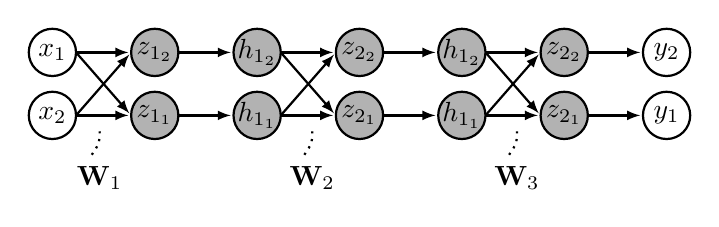
\begin{tikzpicture}[>=spaced latex]
% linear1
\draw [thick] (0,-0.4) circle [radius=0.3] node {$x_2$};
\draw [thick] (0,0.4) circle [radius=0.3] node {$x_1$};
\draw [thick] [nn_edge] (0.3,-0.4) -- (1.0,-0.4);
\draw [thick] [nn_edge] (0.3,0.4) -- (1.0,0.4);
\draw [thick] [nn_edge] (0.3,-0.4) -- (1.0,0.4);
\draw [thick] [nn_edge] (0.3,0.4) -- (1.0,-0.4);
\draw [thick, fill=gray_neuron] (1.3,-0.4) circle [radius=0.3] node {$z_{1_1}$};
\draw [thick, fill=gray_neuron] (1.3,0.4) circle [radius=0.3] node {$z_{1_2}$};
\draw [thick,dotted] (0.5,-0.9)  .. controls (0.6,-0.75) .. (0.6,-0.6);
\draw (0.6,-1.2) node {$\mathbf{W}_1$};

% relu1
\draw [thick] [nn_edge] (1.6,-0.4) -- (2.3,-0.4);
\draw [thick] [nn_edge] (1.6,0.4) -- (2.3,0.4);
\draw [thick, fill=gray_neuron] (2.6,-0.4) circle [radius=0.3] node {$h_{1_1}$};
\draw [thick, fill=gray_neuron] (2.6,0.4) circle [radius=0.3] node {$h_{1_2}$};

% linear2
\draw [thick] [nn_edge] (2.9,-0.4) -- (3.6,0.4);
\draw [thick] [nn_edge] (2.9,0.4) -- (3.6,-0.4);
\draw [thick] [nn_edge] (2.9,-0.4) -- (3.6,-0.4);
\draw [thick] [nn_edge] (2.9,0.4) -- (3.6,0.4);
\draw [thick, fill=gray_neuron] (3.9,-0.4) circle [radius=0.3] node {$z_{2_1}$};
\draw [thick, fill=gray_neuron] (3.9,0.4) circle [radius=0.3] node {$z_{2_2}$};
\draw [thick,dotted] (3.2,-0.9)  .. controls (3.3,-0.75) .. (3.3,-0.6);
\draw (3.3,-1.2) node {$\mathbf{W}_2$};

% relu2
\draw [thick] [nn_edge] (4.2,-0.4) -- (4.9,-0.4);
\draw [thick] [nn_edge] (4.2,0.4) -- (4.9,0.4);
\draw [thick, fill=gray_neuron] (5.2,-0.4) circle [radius=0.3] node {$h_{1_1}$};
\draw [thick, fill=gray_neuron] (5.2,0.4) circle [radius=0.3] node {$h_{1_2}$};

% linear3
\draw [thick] [nn_edge] (5.5,-0.4) -- (6.2,0.4);
\draw [thick] [nn_edge] (5.5,0.4) -- (6.2,-0.4);
\draw [thick] [nn_edge] (5.5,-0.4) -- (6.2,-0.4);
\draw [thick] [nn_edge] (5.5,0.4) -- (6.2,0.4);
\draw [thick, fill=gray_neuron] (6.5,-0.4) circle [radius=0.3] node {$z_{2_1}$};
\draw [thick, fill=gray_neuron] (6.5,0.4) circle [radius=0.3] node {$z_{2_2}$};
\draw [thick,dotted] (5.8,-0.9)  .. controls (5.9,-0.75) .. (5.9,-0.6);
\draw (5.9,-1.2) node {$\mathbf{W}_3$};

% softmax
\draw [thick] [nn_edge] (6.8,-0.4) -- (7.5,-0.4);
\draw [thick] [nn_edge] (6.8,0.4) -- (7.5,0.4);
\draw [thick] (7.8,-0.4) circle [radius=0.3] node {$y_1$};
\draw [thick] (7.8,0.4) circle [radius=0.3] node {$y_2$};
\end{tikzpicture}
%\end{minipage}
}
\caption{An MLP with three linear layers and two outputs, suitable for performing binary softmax regression.}
%\vspace{-1.0cm}
\label{fig:neural_nets:simple_MLP_network2}
\end{figure}

Or expressed in math as follows:
\begin{align}
    \mathbf{z}_1 &= \mathbf{W}_1\mathbf{x} + \mathbf{b}_1 &\triangleleft \quad \texttt{linear}\\
    \mathbf{h}_1 &= \texttt{relu}(\mathbf{z}_1) &\triangleleft \quad \texttt{relu}\\
    \mathbf{z}_2 &= \mathbf{W}_2\mathbf{h}_1 + \mathbf{b}_2 &\triangleleft \quad \texttt{linear}\\
    \mathbf{h}_2 &= \texttt{relu}(\mathbf{z}_2) &\triangleleft \quad \texttt{relu}\\
    \mathbf{z}_3 &= \mathbf{W}_3\mathbf{h}_2 + \mathbf{b}_3 &\triangleleft \quad \texttt{linear}\\
    \mathbf{y} &= \texttt{softmax}(\mathbf{z}_3) &\triangleleft \quad \text{\texttt{softmax}}
\end{align}

% Or in Pytorch-like pseudocode as:
% \begin{figure}[h]
% %\centerline{
% \begin{minipage}{0.5\linewidth}
% \begin{minted}[
% fontsize=\fontsize{8.5}{9},
% frame=single,
% framesep=2.5pt,
% baselinestretch=1.05,
% ]{python}
% # W1, b1, W2, b2 : parameters of the net
% # X : dataset to run through net

% # first define parameterized layers
% fc1 = nn.linear(W1, b1)
% fc2 = nn.linear(W2, b2)

% # then run data through network
% for x in X:
%     z1 = fc1(x)
%     h1 = nn.relu(z1)
%     z2 = fc2(h1)
%     y = nn.softmax(z2)
% \end{minted}
% \end{minipage}
% \cation{Pytorch-like pseudocode for the MLP in Figure \ref{fig:neural_nets:simple_MLP_network2}.}
% %}
% \end{figure}

Now we wish to train this net to classify between two data distributions. The goal is to transform the input distribution into a target distribution that separates the classes, as shown in \fig{\ref{fig:neural_nets_as_data_transformations:goal_of_classifier}}.
\begin{figure}[h]
    \centerline{
    \begin{minipage}{0.28\textwidth}
    \begin{tikzpicture}
        \draw (0, 0) node[inner sep=0] {\includegraphics[width=0.75\linewidth]{figures/neural_nets/binary_classifier_example_training_data2.pdf}};
        \draw (-1.2, 1.2) node {$\mathbf{x}$};
        \draw (0, 1.75) node {Input data};
        %
        
        % neural net mapping
        \draw [thick,->] (2, 0) -- (6.5, 0);
        \def\Nlayers{6}
        \def\layerheight{0.6}
        \def\layerstep{0.3}
        \foreach \x in {1,...,\Nlayers} {
            \draw [fill=white] (\layerstep*\x+3.1,-\layerheight/2) rectangle ++(\layerheight/4,\layerheight);
        }
        %\draw (4.25, 0) node[fill=white] {$?$};
        \draw (4.25, 0.75) node {Series of geometric transformations};
        \draw (4.25, -0.75) node {(i.e., a neural net)};
        %
    \end{tikzpicture}
    \end{minipage}
    \begin{minipage}{0.28\textwidth}
    \begin{tikzpicture}
        %\draw (0, 1) node {$?$};
        %\draw [thick,->] (0, 1) -- (1, 1);
    \end{tikzpicture}
    \end{minipage}
    \begin{minipage}{0.28\textwidth}
    \begin{tikzpicture}
        \draw (0, 0) node[inner sep=0] {\includegraphics[width=0.75\linewidth]{figures/neural_nets/binary_classifier_ex_targets.pdf}};
        \draw (-1.2, 1.2) node {$\mathbf{y}$};
        \draw (0, 1.75) node {Target output};
    \end{tikzpicture}
    \end{minipage}
    }
    \caption{The goal of a neural net classifier is to rearrange the input data distribution to match the target label distribution. (left) Input dataset with two classes in red and blue. (right) Target output (one-hot codes).}
    \label{fig:neural_nets_as_data_transformations:goal_of_classifier}
\end{figure}

In this example, the target output places all the red dots at $(0,1)$ and all the blue dots at $(1,0)$. These are the coordinates of one-hot codes for our two classes. Training the network consists of find the series of geometric transformations that rearrange the input distribution to this target output distribution.

We will visualize how the net transforms the training dataset, layer by layer, at four \index{Checkpoint}{\bf checkpoints} over the course of training.\marginnote{A checkpoint is a record of the parameters at some iteration of training, that is, if iterates of the parameter vector are $\theta^0, \theta^1, \ldots, \theta^T$, then any $\theta^k$ can be recorded as a checkpoint.}[-2.2cm] In \fig{\ref{fig:neural_nets:nn_training_viz}}, we plot this as a 3D visualization of $\mathbb{R}^2 \rightarrow \mathbb{R}^2$ mappings. Each dotted line connects the representation of a datapoint at one layer to its representation at the next. The gray lines show, for each layer, how a square region around the origin gets stretched, rotated, or squished to map to a transformed region on the next layer.
\begin{figure}[h]
    \centerline{
    \includegraphics[width=1.0\linewidth]{./figures/neural_nets/nn_training_viz2.pdf}
    }
    \caption{How a deep net remaps input data layer by layer. The target output is to move all the red points to $(0,1)$ and all the blue points to $(1,0)$ (one-hot codes for the two classes). As training progresses the network gradually achieves this separation.}
    \label{fig:neural_nets:nn_training_viz}
\end{figure}

Of course, ``stretched, rotated, or squished'' is just an intuitive way to think about it, but we can be more precise. The linear layers perform an affine transformation of the space, while the relus project all negative values to the boundaries of the cone whose dimensions are strictly positive. Layer by layer, over the course of training, the net learns to disentangle these two classes and pull the points toward vertices of the one-simplex, achieving a correct classification of the points!


\section{How High-Dimensional Datapoints Get Remapped by Deep Net}
%When the represntation $\mathbf{h}^{(1)i}$ were a two-dimensional vector, then we could visualize this representation for all datapoints $i$ in a dataset as a 2D scatter plot. If the next layer $\mathbf{h}^{(2)i}$ were also two-dimensional, then it would be a different scatter plot, with each datapoint shifted to a new position. Typically, each hidden layer is a high-dimensional vector, so it's non-trivial to visualize datapoints in this space.
What if our data and activations are high-dimensional? The plots above only can visualize 1D and 2D data distributions. Deep representations are typically much higher-dimensional than this, and to visualize them, we need to apply tools from {\bf dimensionality reduction}. These tools project the high-dimensional data to a lower dimensionality, for example 2D, which can be visualized. A common objective is to perform the projection such that the distance between two datapoints in the 2D projection is roughly proportional to their actual distance in the high-dimensional space. In the next plot, \fig{\ref{fig:neural_nets:vit_mapping_plot}}, we use a dimensionality reduction technique called \textbf{t-Distributed Stochastic Neighbor Embedding} \textbf{t-SNE}~\cite{tsne} to visualize how different layers of a modern deep net represent a dataset of images of different semantic classes, where each color represents a different semantic class. The network we are visualizing is of the transformer architecture, and we will learn about all its details in \chap{\ref{chapter:transformers}}. For now, the important things to note are that (1) we are only showing a selected few of the layers (this net actually has dozen of layers) and (2) the embeddings are high-dimensional (in particular, they are 38,400-dimensional) but mapped down to 2D by t-SNE. Therefore, this visualization is just a rough view of what is going on in the net, unlike the visualizations in the previous section, which showed the exact embeddings and every single step of the layer-to-layer transformations.
%The following plot uses a dimensionality reduction technique called t-SNE~\cite{tsne} to visualize how different layers of a deep net represent a dataset of images of different semantic classes, where each color represents a different semantic class:
%The following plot, reproduced from \cite{decaf}, 
% \begin{figure}[h]
%     \centerline{
%     \includegraphics[width=0.6\linewidth]{./figures/neural_nets/decaf_tsne.pdf}
%     }
%     \caption{How a deep image classifier remaps input pixels into a disentangled representation where semantic classes are separated. The t-SNE visualization is taken from \cite{decaf}. \reviewcomment{Replace fish photo, get permission to use tsne image.}}
%     \label{fig:neural_nets:decaf_tsne}
% \end{figure}
\begin{figure}[t]
    \centerline{
    \includegraphics[width=0.375\linewidth]{./figures/neural_nets/vit_mapping_plot.pdf}
    }
    \caption{How a powerful deep net remaps input images into a disentangled representation where semantic classes (shown in different colors) are separated. This deep net is a vision transformer (ViT~\cite{dosovitskiy2020vit}), which we will learn about in \sect{\ref{sec:transformers:ViT_arch}}. It was trained using contrastive language-image pre-training (CLIP~\cite{radford2021learning}, see \sect{\ref{sec:VLMs:CLIP}}). Each \texttt{ViT block} contains multiple layers of neural processing (see \fig{\ref{fig:transformers:ViT_arch}}; we visualize the embeddings right after the first \texttt{token norm} in a block). We apply t-SNE jointly across all shown layers.} %which is size $(NL) \times d$, where $N$ is the number of images, $L$ is the number of layers that are plotted, and $d$ is the dimensionality of each layer (how many neurons it has).}
    \label{fig:neural_nets:vit_mapping_plot}
\end{figure}

Notice that on the first layer, semantic classes are not well separated but by the last layer the representation has {\bf disentangled} the semantic classes so that each class occupies a different part of representational space. This is expected because the final layer in this visualization is near the output of the network, and this network has been trained to output a direct representation of semantics (in particular, this net was trained with contrastive language-image pre-training [CLIP~\cite{radford2021learning}], which is a method for learning semantic representations that we will learn about in \sect{\ref{sec:VLMs:CLIP}}).%, that is, a completely disentangled representation.

\section{Concluding Remarks}
Layer by layer, deep nets transform data from its raw format to ever more abstracted and useful representations. It can be helpful to think about this process as a set of geometric transformations of a data distribution, or as a kind of disentangling where initially messy data gets reorganized so that different data classes become cleanly separated. % PHILLIP
% 
%\setcounter{chapter}{13}
\chapter{Backpropagation}\label{chapter:backpropagation}

\index{Backpropagation}
\section{Introduction}
A key idea of neural nets is to decompose computation into a series of layers. In this chapter we will think of layers as modular blocks that can be chained together into a \index{Computation graph}\textbf{computation graph}. \Fig{\ref{fig:backpropagation:simple_MLP}} shows the computation graph for the two-layer multilayer perceptron (MLP) from \chap{\ref{chapter:neural_nets}}.

\vspace{-0.2cm}
\begin{figure}[h]
\begin{minipage}{.23\textwidth}
\centering
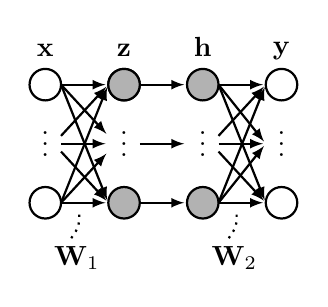
\begin{tikzpicture}[>=spaced latex]
\draw [thick] (0,-0.75) circle [radius=0.2] node[label={$\mathbf{x}$}] at (0,0.85) {};
\draw [thick] (0,0.1) node {$\vdots$};
\draw [thick] (0,0.75) circle [radius=0.2];

\draw [thick,dotted] (0.33,-1.2)  .. controls (0.43,-1.05) .. (0.43,-0.9);
\draw (0.4,-1.45) node {$\mathbf{W}_1$};

\draw [thick] [nn_edge] (0.2,-0.75) -- (0.8,-0.1);
\draw [thick] [nn_edge] (0.2,-0.75) -- (0.8,-0.75);
\draw [thick] [nn_edge] (0.2,-0.75) -- (0.8,0.75);
\draw [thick] [nn_edge] (0.2,-0.1) -- (0.8,-0.75);
\draw [thick] [nn_edge] (0.2,0.0) -- (0.8,0.0);
\draw [thick] [nn_edge] (0.2,0.1) -- (0.8,0.75);
\draw [thick] [nn_edge] (0.2,0.75) -- (0.8,0.75);
\draw [thick] [nn_edge] (0.2,0.75) -- (0.8,-0.75);
\draw [thick] [nn_edge] (0.2,0.75) -- (0.8,0.1);
\draw [thick, fill=gray_neuron] (1,0.75) circle [radius=0.2]  node[label={$\mathbf{z}$}] at (1.0,0.85) {};
\draw [thick] (1,0.1) node {$\vdots$};
\draw [thick, fill=gray_neuron] (1,-0.75) circle [radius=0.2];
\draw [thick] [nn_edge] (1.2,0.75) -- (1.8,0.75);
\draw [thick] [nn_edge] (1.2,0.0) -- (1.8,0.0);
\draw [thick] [nn_edge] (1.2,-0.75) -- (1.8,-0.75);
\draw [thick, fill=gray_neuron] (1,0.75) circle [radius=0.2]  node[label={$\mathbf{h}$}] at (2.0,0.85) {};
\draw [thick, fill=gray_neuron] (2.0,0.75) circle [radius=0.2];
\draw [thick] (2.0,0.1) node {$\vdots$};
\draw [thick, fill=gray_neuron] (2.0,-0.75) circle [radius=0.2];

\draw [thick,dotted] (2.33,-1.2)  .. controls (2.43,-1.05) .. (2.43,-0.9);
\draw (2.4,-1.45) node {$\mathbf{W}_2$};

\draw [thick] [nn_edge] (2.2,-0.75) -- (2.8,-0.75);
\draw [thick] [nn_edge] (2.2,-0.75) -- (2.8,0.75);
\draw [thick] [nn_edge] (2.2,-0.75) -- (2.8,0.0);
\draw [thick] [nn_edge] (2.2,-0.1) -- (2.8,-0.75);
\draw [thick] [nn_edge] (2.2,0.0) -- (2.8,0.0);
\draw [thick] [nn_edge] (2.2,0.1) -- (2.8,0.75);
\draw [thick] [nn_edge] (2.2,0.75) -- (2.8,0.75);
\draw [thick] [nn_edge] (2.2,0.75) -- (2.8,-0.75);
\draw [thick] [nn_edge] (2.2,0.75) -- (2.8,0.0);
\draw [thick] (3.0,-0.75) circle [radius=0.2] node[label={$\mathbf{y}$}] at (3.0,0.8) {};
\draw [thick] (3.0,0.1)  node {$\vdots$};
\draw [thick] (3.0,0.75) circle [radius=0.2];
\end{tikzpicture}
\end{minipage}
%
%
\begin{minipage}{0.77\textwidth}
\centering
\def\layerwidth{1.3}
\begin{tikzpicture}[
cblock/.style={
draw,
fill=comp_graph_node_bcolor,
rectangle, 
inner sep=1.5mm,
minimum width=\layerwidth*0.9 cm,
minimum height=\layerwidth*0.5*0.9 cm,
font=\footnotesize}]
%
\draw [thick] [comp_graph_edge] (\layerwidth*0.5,0) -- (\layerwidth,0);
%\draw (0,0) rectangle ++(1,1);
\draw (\layerwidth*1.5,0) node [cblock] {\texttt{linear}};
\draw [thick] [comp_graph_edge] (\layerwidth*2,0) -- (\layerwidth*3,0);
\draw (\layerwidth*3.5,0) node [cblock] {\texttt{relu}};
\draw [thick] [comp_graph_edge] (\layerwidth*4,0) -- (\layerwidth*5,0);
\draw (\layerwidth*5.5,0) node [cblock] {\texttt{linear}};
\draw [thick] [comp_graph_edge] (\layerwidth*6,0) -- (\layerwidth*6.25,0);

\draw (\layerwidth*0.5,0) node [fill=comp_graph_data_bcolor] {$\mathbf{x}$};
\draw (\layerwidth*2.5,0) node [fill=comp_graph_data_bcolor] {$\mathbf{z}$};
\draw (\layerwidth*4.5,0) node [fill=comp_graph_data_bcolor] {$\mathbf{h}$};
\draw (\layerwidth*6.5,0) node [fill=comp_graph_data_bcolor] {$\hat{\mathbf{y}}$};

\draw (-1,0) node {$\iff$};
\end{tikzpicture}
\end{minipage}
\caption{In this chapter we will visualize neural nets as a sequence of layers, which we call a computation graph.}
\label{fig:backpropagation:simple_MLP}
\end{figure}
\vspace{-0.2cm}

Each {\setlength{\fboxsep}{2pt}\colorbox{comp_graph_node_bcolor}{layer}} takes in some inputs and transforms them into some outputs. We call this the $\texttt{forward}$ pass through the layer. If the layer has parameters, we will consider the parameters to be an \textit{input} to a parameter-free transformation:
\begin{align}
    \xout &= f(\xin,\theta)
\end{align}
Graphically, we will depict the forward operation of a layer like shown below (\fig{\ref{fig:backpropagation:mod_block_forward}}).
\vspace{-0.2cm}
\begin{figure}[h]
\centerline{
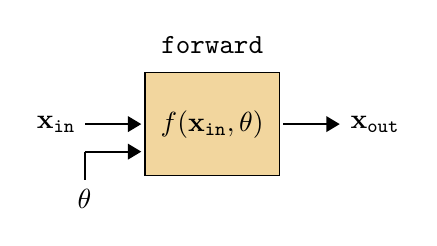
\begin{tikzpicture}%[>=spaced latex]
%
\def\layerwidth{1.8}
%
\draw [thick] [comp_graph_edge] (\layerwidth*0.6,-0.35) -- (\layerwidth,-0.35);
\draw [thick] (\layerwidth*0.6,-0.75) -- (\layerwidth*0.6,-0.35);
\draw [thick] [comp_graph_edge] (\layerwidth*0.5,0) -- (\layerwidth,0);
\draw (\layerwidth*1.5,0) node [fill=comp_graph_node_bcolor,draw, inner sep=2mm, minimum height=1.3cm] {$f(\xin, \theta)$};
\draw [thick] [comp_graph_edge] (\layerwidth*2,0) -- (\layerwidth*2.4,0);
%
\draw (\layerwidth*0.6,-0.95) node [fill=white] {$\theta$};
\draw (\layerwidth*0.4,0) node [fill=comp_graph_data_bcolor] {$\xin$};
\draw (\layerwidth*2.65,0) node [fill=comp_graph_data_bcolor] {$\xout$};
\draw (\layerwidth*1.5,1) node {\texttt{forward}};
%
\end{tikzpicture}
}
\caption{Forward operation of a neural net layer.}
\label{fig:backpropagation:mod_block_forward}
\end{figure}
\vspace{-0.2cm}

% \begin{figure}[h]
% \centering
% \begin{tikzpicture}%[>=spaced latex]
% %
% \def\layerheight{1.0}

% \draw [thick] [comp_graph_edge] (0,0) -- (0,\layerheight);
% %\draw (0,0) rectangle ++(1,1);
% \draw (0,\layerheight*1.5) node [fill=comp_graph_node_bcolor,draw, inner sep=2mm] {$f(\xin)$};
% \draw [thick] [comp_graph_edge] (0,\layerheight*2) -- (0,\layerheight*3);

% \draw (0,\layerheight*0.4) node [fill=comp_graph_data_bcolor] {$\xin$};
% \draw (0,\layerheight*2.4) node [fill=comp_graph_data_bcolor] {$\xout$};

% \end{tikzpicture}
% \label{fig:backpropagation:mod_block}
% \end{figure}

% \begin{figure}[h]
%     \centering
%     \includegraphics[width=0.18\linewidth]{./figures/backpropagation/mod_block.pdf}
%     \label{fig:mod_block}
% \end{figure}

%A graph of computational blocks like this is called a \textbf{computation graph}.

The learning problem is to find the parameters {\setlength{\fboxsep}{2pt}\colorbox{comp_graph_param_bcolor}{$\theta$}} that achieve a desired mapping. Usually we will solve this problem via gradient descent. The question of this chapter is, how do we compute the gradients?
\marginnote{We will use the color \raisebox{1mm}{\colorbox{comp_graph_param_bcolor}{\makebox(0,0){}}} to indicate \textit{free} parameters, which are set via learning and are not the result of any other processing.}[-1.9cm]
%These parameters, along with the input training data, are the leaves in the computation graph.

\textbf{Backpropagation} is an algorithm that efficiently calculates the gradient of the loss with respect to each and every parameter in a computation graph. It relies on a special new operation, called \texttt{backward} that, just like \texttt{forward}, can be defined for each layer, and acts in isolation from the rest of the graph. But first, before we get to defining \texttt{backward}, we will build up some intuition about the key trick backpropagation will exploit.

\section{The Trick of Backpropagation: Reuse of Computation}

To start, we will consider a simple computation graph that is a chain of functions $f_L \circ f_{L-1} \circ \cdots f_2 \circ f_1$, with each function $f_l$ parameterized by $\theta_l$.\marginnote{Such a computation graph could represent an MLP, for example, which we will see in the next section.}[-0.4cm] We aim to optimize the parameters with respect to a loss function $\mathcal{L}$. The loss can be treated as another node in our computation graph, which takes in $\mathbf{x}_L$ (the output of $f_L$) and outputs a scalar $J$, the loss. This computation graph appears as follows (\fig{\ref{fig:backpropagation:composed_modules}}).
\begin{figure}[h]
    \centerline{
    \def\layerwidth{1.2}
    \begin{tikzpicture}[
    cblock/.style={
    draw,
    fill=comp_graph_node_bcolor,
    rectangle, 
    inner sep=1.5mm,
    minimum width=\layerwidth*0.9 cm,
    minimum height=\layerwidth*0.75*0.9 cm}]
    %
    %
    % draw f nodes
    \def\fnames {{"$f_0$","$f_1$","$f_2$","$f_{L-1}$","$f_L$"}}
    \foreach \x in {1,2,3,4} {
        \pgfmathparse{\fnames[\x]};
        \draw ($(\layerwidth*2*\x-\layerwidth+\layerwidth*0.5,0)$) node [cblock] {\pgfmathresult};
    }
    % draw data arrows
    \draw [thick] [comp_graph_edge] (\layerwidth*0.5,0) -- (\layerwidth,0);
    \foreach \x in {1,2,3,4} {
        % data arrow
        \draw [thick] [comp_graph_edge] (\layerwidth*2*\x,0) -- (\layerwidth*2*\x+\layerwidth,0);
    }
    \draw [thick] [comp_graph_edge] (\layerwidth*10,0) -- (\layerwidth*10.25,0);
    %
    % draw param arrows
    \foreach \x in {0,1,2,3} {
        \draw [thick] [comp_graph_edge] (\layerwidth*2*\x+\layerwidth*0.6,-0.35) -- (\layerwidth*2*\x+\layerwidth,-0.35);
        \draw [thick] (\layerwidth*2*\x+\layerwidth*0.6,-0.75) -- (\layerwidth*2*\x+\layerwidth*0.6,-0.35);
    }
    %
    % draw data and params
    \def\datanames {{"$\mathbf{x}_0$","$\mathbf{x}_1$","$\cdots$","$\mathbf{x}_{L-1}$","$\mathbf{x}_L$"}}
    \def\paramnames {{"$\theta_1$","$\theta_2$","$\theta_{L-1}$","$\theta_{L}$"}}
    \foreach \x in {0,1,2,3,4} {
        \pgfmathparse{\datanames[\x]};
        \draw ($(\layerwidth*2*\x+\layerwidth*0.5,0)$) node [fill=comp_graph_data_bcolor] {\pgfmathresult};
        %
    };
    \foreach \x in {0,1,2,3} {
        \pgfmathparse{\paramnames[\x]};
        \draw ($(\layerwidth*2*\x+\layerwidth*0.5,-0.95)$) node [fill=comp_graph_param_bcolor] {\pgfmathresult};
    };
    %
    % loss node
    \draw (\layerwidth*9.5,0) node [cblock, fill=comp_graph_loss_node_bcolor] {$\mathcal{L}$};
    \draw (\layerwidth*10.4,0) node [fill=comp_graph_data_bcolor] {$J$};
    %
    \draw (6.3,-1.4) node {$\underbrace{\quad\quad\quad\quad\quad\quad\quad\quad\quad\quad\quad\quad\quad\quad\quad\quad\quad\quad\quad\quad\quad\quad\quad\quad\quad\quad\quad\quad\quad\quad\quad\quad\quad\quad\quad}$};
    \draw (6.3,-1.9) node [scale=1.25] {$\frac{\partial J}{\partial \theta_1}$};
    \draw (7.6,-2.4) node {$\underbrace{\quad\quad\quad\quad\quad\quad\quad\quad\quad\quad\quad\quad\quad\quad\quad\quad\quad\quad\quad\quad\quad\quad\quad\quad\quad\quad\quad\quad}$};
    \draw (7.6,-2.9) node [scale=1.25] {$\frac{\partial J}{\partial \theta_2}$};
    %
    \end{tikzpicture}
    }
    \caption{Basic sequential computation graph.}
    \label{fig:backpropagation:composed_modules}
\end{figure}
\marginnote{This computation graph is a narrow tree; the parameters live on branches of length 1. This can be easier to see when we plot it with data and parameters as nodes and edges as the functions:
\medbreak
\centerline{
\includegraphics[width=0.45\linewidth]{./figures/backpropagation/cgraph_tree.pdf}
}
The parameters, along with the input training data, are the leaves of the computation graph.
}[2.4cm]

Our goal is to update all the values highlighted in blue: $\theta_1$, $\theta_2$, and so forth. To do so we need to compute the gradients $\frac{\partial J}{\partial \theta_1}$, $\frac{\partial J}{\partial \theta_2}$, etc. Each of these gradients can be calculated via the chain rule. Here is the chain rule written out for the gradients for $\theta_1$ and $\theta_2$:
\begin{align}
    \frac{\partial J}{\partial \theta_1} &= \highlight[shared_term_color]{\frac{\partial J}{\partial \mathbf{x}_L}\frac{\partial \mathbf{x}_L}{\partial \mathbf{x}_{L-1}} \cdots \frac{\partial \mathbf{x}_3}{\partial \mathbf{x}_2}} \frac{\partial \mathbf{x}_2}{\mathbf{x}_1}\frac{\partial \mathbf{x}_1}{\partial \mathbf{\theta}_1}\\
    \frac{\partial J}{\partial \theta_2} &=  \highlight[shared_term_color]{\frac{\partial J}{\partial \mathbf{x}_{L}}\frac{\partial \mathbf{x}_L}{\partial \mathbf{x}_{L-1}} \cdots \frac{\partial \mathbf{x}_3}{\partial \mathbf{x}_2}} \frac{\partial \mathbf{x}_2}{\partial \theta_2}
\end{align}
Rather than evaluating both equations separately, we notice that all the terms in each gray box are shared. We only need to evaluate this product once, and then can use it to compute both $\frac{\partial J}{\partial \theta_1}$ and $\frac{\partial J}{\partial \theta_2}$. Now notice that this pattern of reuse can be applied in the same way for $\theta_3$, $\theta_4$, and so on. This is the whole trick of backpropagation: rather than computing each layer's gradients independently, observe that they share many of the same terms, so we might as well calculate each shared term once and reuse them. \marginnote{This strategy, in general, is called {\bf dynamic programming}.}[-0.6cm]

%\section{\texttt{Backward} for a generic layer}
\section{Backward for a Generic Layer}
To come up with a general algorithm for reusing all the shared computation, we will first look at one generic layer in isolation, and see what we need in order to update its parameters (\fig{\ref{fig:backpropagation:generic_layer_g_L}}).
\begin{figure}[h]
\centerline{
\begin{tikzpicture}%[>=spaced latex]
%
\def\layerwidth{1.8}
%
\draw [thick] [comp_graph_edge] (\layerwidth*0.6,-0.35) -- (\layerwidth,-0.35);
\draw [thick] (\layerwidth*0.6,-0.75) -- (\layerwidth*0.6,-0.35);
\draw [thick] [comp_graph_edge] (\layerwidth*0.5,0) -- (\layerwidth,0);
\draw (\layerwidth*1.5,0) node [fill=comp_graph_node_bcolor,draw, inner sep=2mm, minimum height=1.3cm] {$f(\xin, \theta)$};
\draw [thick] [comp_graph_edge] (\layerwidth*2,0) -- (\layerwidth*2.4,0);
%
\draw (\layerwidth*0.6,-0.95) node [fill=comp_graph_param_bcolor] {$\theta$};
\draw (\layerwidth*0.4,0) node [fill=comp_graph_data_bcolor] {$\xin$};
\draw (\layerwidth*2.65,0) node [fill=comp_graph_data_bcolor] {$\xout$};
\draw (\layerwidth*3,0) node {$\cdots$};
\draw [thick] [comp_graph_edge] (\layerwidth*3.2,0) -- (\layerwidth*3.6,0);
\draw (\layerwidth*3.8,0) node {$J$};
\draw [thick] [comp_graph_edge] (-0.2*\layerwidth,0) -- (0.2*\layerwidth,0);
\draw (-0.4*\layerwidth,0) node {$\cdots$};
%
\draw (2.8,-1.4) node {$\underbrace{\quad\quad\quad\quad\quad\quad\quad\quad\quad\quad\quad\quad\quad}$};
\draw (2.8,-1.9) node [scale=1.2] {$\localgrad$};
\draw (5.8,-1.8) node {$\underbrace{\quad\quad\quad\quad\quad\quad\quad}$};
\draw (5.8,-2.3) node [scale=1.2] {$\costgradout$};
\draw (3.8,-2.6) node {$\underbrace{\quad\quad\quad\quad\quad\quad\quad\quad\quad\quad\quad\quad\quad\quad\quad\quad\quad\quad\quad}$};
\draw (3.8,-3.1) node [scale=1.2] {$\costgradin$};
%
\end{tikzpicture}
}
\caption{A generic layer in the computation graph. The braces represent the part of the computation graph we need to consider in order to evaluate $\costgradout$, $\localgrad$, and $\costgradin$.}
\label{fig:backpropagation:generic_layer_g_L}
\end{figure}

% Here we have introduced two new shorthands, $\localgrad$ and $\costgrad$ -- these represent arrays of partial derivatives, defined below, and they are the key arrays we need to keep track of to do backprop. They are defined as:
% %To update $\theta$ for this layer, we just need to know $\frac{\partial J}{\partial \theta}$
% %This strategy involves two key matrices: 1) the vector of derivatives of the cost $J$ w.r.t to each layer's inputs, and 2) the matrix of derivatives of the outputs of each layer with respect to its inputs. We define shorthand for these below:
% \marginnote{All these arrays represent the gradient \textit{at a single operating point} --  that of the current value of the data and parameters.}[1cm]
% \begin{align}
%     \costgrad &\triangleq \frac{\partial J}{\partial [\xin, \xout, \theta]} &&\quad\quad \triangleleft \quad \text{grad of cost}\\
%      &\quad\quad \costgradxin \triangleq \frac{\partial J}{\partial \xin} &&\quad\quad \triangleleft \quad \text{... w.r.t. layer inputs} \quad [1 \times |\xin|]\\
%      &\quad\quad \costgradxout \triangleq \frac{\partial J}{\partial \xout} &&\quad\quad \triangleleft \quad \text{... w.r.t. layer outputs} \quad [1 \times |\xout|]\\
%      &\quad\quad \costgradtheta \triangleq \frac{\partial J}{\partial \theta} &&\quad\quad \triangleleft \quad \text{... w.r.t. layer params} \quad [1 \times |\theta|]\\
%     \localgrad &\triangleq \frac{\partial \xout}{\partial [\xin, \theta]} &&\quad\quad \triangleleft \quad \text{grad of layer}\\
%     &\quad\quad \localgradx \triangleq \frac{\partial \xout}{\partial \xin} &&\quad\quad \triangleleft \quad \text{... w.r.t. layer input data} \quad [|\xout| \times |\xin|]\\
%     &\quad\quad \localgradtheta \triangleq \frac{\partial \xout}{\partial \theta} &&\quad\quad \triangleleft \quad \text{... w.r.t. layer params} \quad [|\xout| \times |\theta|]
%     %\mathbf{F}_l &\triangleq \frac{\partial \mathbf{x}_{l}}{\partial \mathbf{x}_{l-1}} = \frac{\partial f_l(\mathbf{x}_{l-1})}{\partial \mathbf{x}_{l-1}} &\quad\quad \triangleleft \quad [N \times M]
% \end{align}

% Computing $\localgrad$ is an entirely local process: for each layer, we just need to know the functional form of its derivative, $f^{\prime}$, which we then evaluate at the operating point $[\xin, \theta]$ to obtain $\localgrad = f^{\prime}(\xin,\theta)$.

% Computing $\costgrad$ is a bit trickier; it requires evaluating the chain rule, and depends on all the subsequent layers of processing, that come between the current layer and $J$. However, this can be computed iteratively: once we know $\costgrad_l$, for some layer $l$, computing $\costgrad_{l-1}$ is just one more matrix multiply! This can be summarized with the following recurrence relation:
% \begin{align}
%     \costgrad_{\texttt{in}} &= \costgrad_{\texttt{out}}\localgrad^{\mathbf{x}} &&\quad\quad \triangleleft \quad \text{``backpropagation of errors"} \label{eqn:backpropagation:backward}
% \end{align}
% This recurrence is essence of backprop: it sends ``error signals" (gradients) backwards through the network, starting at the last layer and iteratively applying Equation \ref{eqn:backpropagation:backward} to
% compute $\costgrad$ for each previous layer.
% \marginnote{Deep learning libraries like Pytorch have a \texttt{.grad} field associated with each variable (data, activations, parameters). This field reprsents $\frac{\partial J}{\partial v}$ for each variable $v$.}[-0.4cm]

% To do gradient-based learning, we need to compute the gradient of the cost w.r.t. the parameters, i.e. $\costgradtheta$. This gives us the parameter \texttt{update} step in gradient descent: 
% \begin{align}
%     \theta^{i+1} &\leftarrow \theta^{i} - \eta (\costgradtheta)^T &&\quad\quad \triangleleft \quad \texttt{update} \label{eqn:backpropagation:djdtheta}
% \end{align}
% \marginnote{The transpose is because, by convention $\theta$ is a column vector while $\costgradtheta = \frac{\partial J}{\partial \theta}$ is a row vector; see Appendix.}[-0.4cm]

% %These arrays give a simple formula for computing the gradient we need -- $\frac{\partial J}{\partial \theta}$ -- in order to \texttt{update} $\theta$ to minimize the cost:
% %\begin{align}
% %    \frac{\partial J}{\partial \theta_l} = \costgrad_l\localgrad^{\theta}_l \quad\quad \triangleleft \quad [1 \times |\xout|]\cdot[|\xout| \times |\theta|] \rightarrow [1 \times \theta]] \label{eqn:backpropagation:param_update}
% %\end{align}

% %The remaining question is just: how do we get $\costgrad_l$ and $\localgrad^{\theta}_l$ for layer $l$? 

% Now, observe that if we already knew $\costgradxout$, then computing $\costgradtheta$ would be easy, it would just be the following matrix product:
% \begin{align}
%     \costgradtheta = \frac{\partial J}{\partial \theta} = \frac{\partial J}{\partial \xout} \frac{\partial \xout}{\partial \theta} = \costgradxout \localgradtheta
% \end{align}

Here we have introduced two new shorthands, $\localgrad$ and $\costgrad$; these represent arrays of partial derivatives, defined below, and they are the key arrays we need to keep track of to do backprop. They are defined as:
%To update $\theta$ for this layer, we just need to know $\frac{\partial J}{\partial \theta}$
%This strategy involves two key matrices: 1) the vector of derivatives of the cost $J$ w.r.t to each layer's inputs, and 2) the matrix of derivatives of the outputs of each layer with respect to its inputs. We define shorthand for these below:
\marginnote{All these arrays represent the gradient \textit{at a single operating point}, namely that of the current value of the data and parameters.}[0.9cm]
\begin{align}
    %\costgrad &\triangleq \frac{\partial J}{\partial [\xin, \xout]} &&\quad\quad \triangleleft \quad \text{grad of cost}\\
    % &\quad\quad \costgradin \triangleq \frac{\partial J}{\partial \xin} &&\quad\quad \triangleleft \quad \text{... w.r.t. layer input data} \quad [1 \times |\xin|]\\
    % &\quad\quad \costgradout \triangleq \frac{\partial J}{\partial \xout} &&\quad\quad \triangleleft \quad \text{... w.r.t. layer outputs} \quad [1 \times |\xout|]\\
    \costgradl &\triangleq \frac{\partial J}{\partial \mathbf{x}_l} &&\quad\quad \triangleleft \quad \text{grad of cost with respect to } \mathbf{x}_l \quad [1 \times |\mathbf{x}_l|]\\
    \localgrad &\triangleq \frac{\partial \xout}{\partial [\xin, \theta]} &&\quad\quad \triangleleft \quad \text{grad of layer}\\
    &\quad\quad \localgrad^{\mathbf{x}} \triangleq \frac{\partial \xout}{\partial \xin} &&\quad\quad \triangleleft \quad \text{\quad with respect to layer input data} \quad [|\xout| \times |\xin|]\\
    &\quad\quad \localgrad^{\theta} \triangleq \frac{\partial \xout}{\partial \theta} &&\quad\quad \triangleleft \quad \text{\quad with respect to layer params} \quad [|\xout| \times |\theta|]
    %\mathbf{F}_l &\triangleq \frac{\partial \mathbf{x}_{l}}{\partial \mathbf{x}_{l-1}} = \frac{\partial f_l(\mathbf{x}_{l-1})}{\partial \mathbf{x}_{l-1}} &\quad\quad \triangleleft \quad [N \times M]
\end{align}

These arrays give a simple formula for computing the gradient we need, that is, $\frac{\partial J}{\partial \theta}$, in order to \texttt{update} $\theta$ to minimize the cost:
%\begin{align}
%    \frac{\partial J}{\partial \theta_l} = \costgrad_l\localgrad^{\theta}_l \quad\quad \triangleleft \quad [1 \times |\xout|]\cdot[|\xout| \times |\theta|] \rightarrow [1 \times \theta]] \label{eqn:backpropagation:param_update}
%\end{align}
\begin{align}
    \frac{\partial J}{\partial \theta} &= \underbrace{\frac{\partial J}{\partial \xout}}_{\costgradout} \underbrace{\frac{\partial \xout}{\partial \theta}}_{\localgradtheta} = \costgradout\localgradtheta\\
    \theta^{i+1} &\leftarrow \theta^{i} - \eta \Big(\frac{\partial J}{\partial \theta}\Big)^\transpose &&\quad\quad \triangleleft \quad \texttt{update} \label{eqn:backpropagation:djdtheta}
\end{align}
\marginnote{The transpose is because, by convention, $\theta$ is a column vector while $\frac{\partial J}{\partial \theta}$ is a row vector; see the Notation section prior to chapter 1.}[-0.5cm]

The remaining question is clear: how do we get $\costgrad_l$ and $\localgrad^{\theta}_l$ for each layer $l$? 

Computing $\localgrad$ is an entirely local process: for each layer, we just need to know the functional form of its derivative, $f^{\prime}$, which we then evaluate at the operating point $[\xin, \theta]$ to obtain $\localgrad = f^{\prime}(\xin,\theta)$.

Computing $\costgrad$ is a bit trickier; it requires evaluating the chain rule, and depends on all the layers between $\xout$ and $J$. However, this can be computed iteratively: once we know $\costgrad_l$, computing $\costgrad_{l-1}$ is just one more matrix multiply! This can be summarized with the following recurrence relation:
\begin{align}
    \costgrad_{\texttt{in}} &= \costgrad_{\texttt{out}}\localgrad^{\mathbf{x}} &&\quad\quad \triangleleft \quad \text{backpropagation of errors}
    \label{eqn:backpropagation:backward}
\end{align}
This recurrence is essence of backprop: it sends error signals (gradients) backward through the network, starting at the last layer and iteratively applying \eqn{\ref{eqn:backpropagation:backward}} to
compute $\costgrad$ for each previous layer.
\marginnote{Deep learning libraries like Pytorch have a \texttt{.grad} field associated with each variable (data, activations, parameters). This field represents $\frac{\partial J}{\partial v}$ for each variable $v$.}[-0.8cm]


We are finally ready to define the full \texttt{backward} function promised at the beginning of this chapter! It consists of the following operation, shown in \fig{\ref{fig:backpropagation:mod_block_backward}}, which has three inputs ($\xin, \theta, \costgrad_{\texttt{out}}$) and two outputs ($\costgrad_{\texttt{in}}$ and $\frac{\partial J}{\partial \theta}$).
\begin{figure}[h]
\centerline{
\begin{tikzpicture}%[>=spaced latex]
%
\def\layerwidth{1.8}
%
\draw [thick] [comp_graph_edge] (0.4,0.6) -- (\layerwidth*0.6,0.6);
\draw [thick] [comp_graph_edge] (\layerwidth*0.6,0) -- (0.4,0);
\draw [thick] [comp_graph_edge] (0.5,-0.6) -- (0.5,-0.95);
\draw [thick] (\layerwidth*0.6,-0.6) -- (0.5,-0.6);
\draw (\layerwidth*1.5,0) node [fill=comp_graph_node_bcolor,draw, inner sep=2mm, minimum height=1.8cm, minimum width=3.0cm] {};
\draw (\layerwidth*1.5,1.2) node {\texttt{backward}};
\draw (\layerwidth*1.5,0.6) node  {$\localgrad = f^{\prime}(\xin,\theta)$};
\draw (\layerwidth*1.5,0) node  {$\costgrad_{\texttt{in}} = \costgrad_{\texttt{out}}\localgrad^{\mathbf{x}}$};
\draw (\layerwidth*1.5,-0.6) node  {$\frac{\partial J}{\partial \theta} = \costgrad_{\texttt{out}}\localgrad^{\theta}$};
\draw [thick] [comp_graph_edge] (\layerwidth*2.8,0) -- (\layerwidth*2.4,0);
%
\draw (0.5,-1.3) node [fill=comp_graph_param_grad_bcolor] {$\frac{\partial J}{\partial \theta}$};
\draw (-0.2,0.6) node [fill=comp_graph_data_bcolor] {$\xin, \theta$};
\draw (0,0) node [fill=comp_graph_data_bcolor] {$\costgrad_{\texttt{in}}$};
\draw (\layerwidth*3,0) node [fill=comp_graph_data_bcolor] {$\costgrad_{\texttt{out}}$};
%
\end{tikzpicture}
}
\caption{\texttt{backward} for a generic layer. We use the color \raisebox{1mm}{\colorbox{comp_graph_param_grad_bcolor}{\makebox(0,0){}}} to indicate parameter gradients.}
\label{fig:backpropagation:mod_block_backward}
\end{figure}

% For any $\frac{\partial J}{\partial \theta_l}$, we have:
% \begin{align}
%     \frac{\partial J}{\partial \theta_l} = \frac{\partial J}{\partial \mathbf{x}_l}\frac{\partial \mathbf{x}_l}{\partial \theta_l}
% \end{align}
% This says that all the parameter updates can be computed with just one further matrix multiply once we know $\frac{\partial J}{\partial \mathbf{x}_l}$ for all $l$. Now, the trick is to work backwards to compute all the $\frac{\partial J}{\partial \mathbf{x}_l}$, because:
% \begin{align}
%     \frac{\partial J}{\partial \mathbf{x}_l} = \frac{\partial J}{\partial \mathbf{x}_{l+1}}\frac{\partial \mathbf{x}_{l+1}}{\partial \mathbf{x}_l}
% \end{align}
% So, once we know $\frac{\partial J}{\partial \mathbf{x}_{l+1}}$ we can compute $\frac{\partial J}{\partial \mathbf{x}_{l}}$ with just one additional matrix multiply.

%The value of the blue terms is $\frac{\partial j}{\partial \mathbf{x}_2}$. Once we have calculated this value, we can 

%Indeed, once we've computed $\frac{\partial \mathbf{x}_{L}}{\partial \mathbf{x}_{l}}$, we can compute $\frac{\partial \mathbf{x}_{L}}{\partial \mathbf{x}_{l-1}}$ with just one more multiply:
%\begin{align}
%    \frac{\partial \mathbf{x}_{L}}{\partial \mathbf{x}_{l-1}} = \frac{\partial \mathbf{x}_{L}}{\partial \mathbf{x}_{l}} \frac{\partial \mathbf{x}_{l}}{\partial \mathbf{x}_{l-1}}
%\end{align}

%\section{Backprop through chains}


% \begin{align}
%     \xout &= f(\xin,\theta) &&\quad\quad \triangleleft \quad \texttt{forward}\\
%     \costgrad_{\texttt{in}} &= \costgrad_{\texttt{out}}\localgrad^{\mathbf{x}} &&\quad\quad \triangleleft \quad \texttt{backward}
% \end{align}

% And then update parameters:
% \begin{align}
%     \frac{\partial J}{\partial \theta} &= \costgrad_{\texttt{out}}\localgrad^{\theta} &&\quad\quad \triangleleft \quad \texttt{update}
% \end{align}


\section{The Full Algorithm: Forward, Then Backward}
We are ready now to define the full backprop algorithm. In the last section we saw that we can easily compute the gradient update for $\theta_l$ once we have computed $\localgrad_l$ and $\costgrad_l$.\marginnote{The $\costgrad_l$ and $\localgrad_l$ are the $\costgrad$ and $\localgrad$ arrays for layer $l$.}[-0.0cm]

So, we just need to order our operations so that when we get to updating layer $l$ we have these two arrays ready. The way to do it is to first compute a \textbf{forward pass} through the entire network, which means starting with input data $\mathbf{x}_0$ and evaluating layer by layer to produce the sequence $\mathbf{x}_0, \mathbf{x}_1, \ldots, \mathbf{x}_L$. \Fig{\ref{fig:backpropagation:forward_pass}} shows what the forward pass looks like.
\begin{figure}[h]
    \centerline{
    \def\layerwidth{1.3}
    \begin{tikzpicture}[
    cblock/.style={
    draw,
    fill=comp_graph_node_bcolor,
    rectangle, 
    inner sep=1.5mm,
    minimum width=\layerwidth*0.9 cm,
    minimum height=\layerwidth*0.75*0.9 cm}]
    %
    %
    % draw f nodes
    \def\fnames {{"$f_0$","$f_1$","$f_2$","$f_{L-1}$","$f_L$"}}
    \foreach \x in {1,2,3,4} {
        \pgfmathparse{\fnames[\x]};
        \draw ($(\layerwidth*2*\x-\layerwidth+\layerwidth*0.5,0)$) node [cblock] {\pgfmathresult};
    }
    % draw data arrows
    \draw [thick] [comp_graph_edge_forward] (\layerwidth*0.5,0) -- (\layerwidth,0);
    \foreach \x in {1,2,3,4} {
        % data arrow
        \draw [thick] [comp_graph_edge_forward] (\layerwidth*2*\x,0) -- (\layerwidth*2*\x+\layerwidth,0);
    }
    %\draw [thick] [comp_graph_edge_forward] (\layerwidth*10,0) -- (\layerwidth*10.25,0);
    %
    % draw param arrows
    \foreach \x in {0,1,2,3} {
        \draw [thick] [comp_graph_edge_forward] (\layerwidth*2*\x+\layerwidth*0.6,-0.35) -- (\layerwidth*2*\x+\layerwidth,-0.35);
    }
    %
    % draw data and params
    \def\datanames {{"$\mathbf{x}_0$","$\mathbf{x}_1$","$\cdots$","$\mathbf{x}_{L-1}$","$\mathbf{x}_L$"}}
    \def\paramnames {{"$\theta_1$","$\theta_2$","$\theta_{L-1}$","$\theta_{L}$"}}
    \foreach \x in {0,1,2,3,4} {
        \pgfmathparse{\datanames[\x]};
        \draw ($(\layerwidth*2*\x+\layerwidth*0.5,0)$) node [fill=white] {\pgfmathresult};
        %
    };
    \foreach \x in {0,1,2,3} {
        \pgfmathparse{\paramnames[\x]};
        \draw ($(\layerwidth*2*\x+\layerwidth*0.5,-0.4)$) node [fill=white] {\pgfmathresult};
    };
    %
    % loss node
    \draw (\layerwidth*9.5,0) node [cblock, fill=comp_graph_loss_node_bcolor] {$\mathcal{L}$};
    %\draw (\layerwidth*10.4,0) node [fill=comp_graph_data_bcolor] {$J$};
    %
    %\draw (\layerwidth*5.5,1.0) node {\textbf{Forward pass}};
    %
    \end{tikzpicture}
    }
    \caption{Forward pass.}
    \label{fig:backpropagation:forward_pass}
\end{figure}
\marginnote{We use the color \raisebox{1mm}{\colorbox{forwardpropcolor}{\makebox(0,0){}}} for data/activations being passed forward through the network.}[2.0cm]

%We need this sequence because, in general, $\localgrad$ for a layer will be a function of $\xin$ and $\theta$ for that layer -- so we need the full sequence of inputs and outputs to each layer to get compute the full sequence $\localgrad_1, \localgrad_2, \ldots$. 

Next, we compute a \textbf{backward pass}, iteratively evaluating the $\costgrad$'s and obtaining the sequence $\costgrad_L, \costgrad_{L-1}, \ldots$, as well as the parameter gradients for each layer (\fig{\ref{fig:backpropagation:backward_pass}}). %Remember that to compute $\costgrad$ for a layer, we need $\localgrad$ for that layer, so on the
\begin{figure}[h]
    \centerline{
    \def\layerwidth{1.3}
    \begin{tikzpicture}[
    cblock/.style={
    draw,
    fill=comp_graph_node_bcolor,
    rectangle, 
    inner sep=1.5mm,
    minimum width=\layerwidth*0.9 cm,
    minimum height=\layerwidth*0.75*0.9 cm}]
    %
    %
    % draw f nodes
    \def\fnames {{"$f^{\prime}_0$","$f^{\prime}_1$","$f^{\prime}_2$","$f^{\prime}_{L-1}$","$f^{\prime}_L$"}}
    \foreach \x in {1,2,3,4} {
        \pgfmathparse{\fnames[\x]};
        \draw ($(\layerwidth*2*\x-\layerwidth+\layerwidth*0.5,0)$) node [cblock] {\pgfmathresult};
    }
    % draw data arrows
    \draw [thick] [comp_graph_edge_backward] (\layerwidth,0) -- (\layerwidth*0.7,0);
    \foreach \x in {1,2,3,4} {
        % data arrow
        \draw [thick] [comp_graph_edge_backward] (\layerwidth*2*\x+\layerwidth,0) -- (\layerwidth*2*\x,0);
    }
    \draw [thick] [comp_graph_edge_backward] (\layerwidth*10.25,0) -- (\layerwidth*10,0);
    %
    % draw data and params
    \def\datanames {{"$\costgrad_0$","$\costgrad_1$","$\cdots$","$\costgrad_{L-1}$","$\costgrad_L$"}}
    \def\paramnames {{"$\frac{\partial J}{\partial \theta_1}$","$\frac{\partial J}{\partial \theta_2}$","$\frac{\partial J}{\partial \theta_{L-1}}$","$\frac{\partial J}{\partial \theta_{L}}$"}}
    \foreach \x in {0,1,2,3,4} {
        \pgfmathparse{\datanames[\x]};
        \draw ($(\layerwidth*2*\x+\layerwidth*0.5,0)$) node [fill=comp_graph_data_bcolor] {\pgfmathresult};
        %
    };
    \foreach \x in {0,1,2,3} {
        \pgfmathparse{\paramnames[\x]};
        \draw ($(\layerwidth*2*\x+\layerwidth*0.5,-0.5)$) node [fill=white] {\pgfmathresult};
    };
    % draw param arrows
    \foreach \x in {0,1,2,3} {
        \draw [thick] [comp_graph_edge_backward] (\layerwidth*2*\x+\layerwidth,-0.35) -- (\layerwidth*2*\x+\layerwidth*0.8,-0.35);
    }
    %
    % loss node
    \draw (\layerwidth*9.5,0) node [cblock, fill=comp_graph_loss_node_bcolor] {$\mathcal{L}^{\prime}$};
    \draw (\layerwidth*10.4,0) node [fill=comp_graph_data_bcolor] {$1$};
    %
    %\draw (\layerwidth*5.5,1.0) node {\textbf{Backward pass}};
    %
    \end{tikzpicture}
    }
    \caption{Backward pass.}
    \label{fig:backpropagation:backward_pass}
\end{figure}
\marginnote{We use the color \raisebox{1mm}{\colorbox{backwardpropcolor}{\makebox(0,0){}}} for data/activation gradients being passed backward through the network.}[2cm]

%Finally, we have all the arrays necessary to compute the gradients $\frac{\partial J}{\partial \theta_l}$ for all $l$ and update all the parameters in the computation graph. 
%Finally, we update our parameters based on the gradients $\frac{\partial J}{\partial \theta_l}$, and repeat. 
The full algorithm is summarized in \algref{\ref{alg:backpropagation:backprop_for_chains}}. %A graphical depiction is given in Figure \ref{fig:backpropagation:backprop_alg_diagram}.

\begin{algorithm}[h]
\SetAlgoVlined
\DontPrintSemicolon
%\marginnote{{\bf Algorithm \ref{alg:backpropagation:backprop_for_chains}}: A simple version of the backpropagation algorithm. This will work for the computation graphs we have seen so far, which consist of a series of layers, $f_1 \circ \ldots \circ f_L$, with no merging or branching (see \sect{\ref{sec:backpropagation:branch_and_merge}} for how to handle more complicated graphs with merge and branch operations).}
\caption{{\bf Algorithm \ref{alg:backpropagation:backprop_for_chains}}: Backpropagation (for chain computation graphs). A simple version of the backpropagation algorithm. This will work for the computation graphs we have seen so far, which consist of a series of layers, $f_1 \circ \ldots \circ f_L$, with no merging or branching (see \sect{\ref{sec:backpropagation:branch_and_merge}} for how to handle more complicated graphs with merge and branch operations).}
\fakealgorithmcaption{}
\label{alg:backpropagation:backprop_for_chains}
{\bf Input:} parameter vector $\theta = \{\theta_l\}_{l=1}^L$, $f_1, \ldots, f_L$, $f^{\prime}_1, \ldots, f^{\prime}_L$, training datapoint $\{\mathbf{x}_0,\mathbf{y}\}$, Loss function $\mathcal{L}: \mathbb{R}^N \rightarrow \mathbb{R}$\;
{\bf Output:} gradient direction $\frac{\partial J}{\partial \theta} = \Big\{\frac{\partial J}{\partial \theta_l}\Big\}_{l=1}^L$ \;
\;
\textbf{Forward pass:}\;
\For{\upshape $l=1, \dots, L$} {
    $\mathbf{x}_l = f_l(\mathbf{x}_{l-1}, \theta_l)$\;
}
%$J = \mathcal{L}(\mathbf{x}_L,y)$\;
\;
\textbf{Backward pass:}\;
$\costgrad_L = \mathcal{L}^{\prime}(\mathbf{x}_L,y)$\;
\For{\upshape $l=L, \dots, 1$} {
    $\localgrad_{l} = f_l^{\prime}(\mathbf{x}_{l-1},\theta_l)$\;
    $\costgrad_{l-1} = \costgrad_{l}\localgrad^{\mathbf{x}}_{l}$\;
    $\frac{\partial J}{\partial \theta_l} = \costgrad_{l}\localgrad^{\theta}_{l}$\;
}
\end{algorithm}

\section{Backpropagation Over Data Batches}
So far, we have only examined computing the gradient of the loss for a single datapoint, $\mathbf{x}$. As you may recall from \chaps{\ref{chapter:intro_to_learning}} and \ref{chapter:gradient_descent}, the total cost function we wish to minimize will typically be the \textit{average} of the losses over \textit{all} the datapoints in a training set, $\{\mathbf{x}^{(i)}\}_{i=1}^N$. However, once we know how to compute the gradient for a single datapoint, we can easily compute the gradient for the whole dataset, due to the following identity:
\begin{align}
    \frac{\partial \frac{1}{N}\sum_{i=1}^N J_i(\theta)}{\partial \theta} = \frac{1}{N} \sum_{i=1}^N \frac{\partial J_i(\theta)}{\partial \theta}\label{eqn:backpropagation:average_of_gradients}
\end{align}
\marginnote{The gradient of a sum of terms is the sum of the gradients of each term.}[-1.0cm]
where $J_i(\theta)$ is the loss for a single datapoint $\mathbf{x}^{(i)}$. Therefore, to compute a gradient update for an algorithm like stochastic gradient descent (\sect{\ref{sec:gradient_descent:SGD}}), we apply backpropagation in batch mode, that is, we run it over each datapoint in our batch (which can be done in parallel) and then average the results.

In the remaining sections, we will still focus only on the case of backpropagation for the loss at a single datapoint. As you read on, keep in mind that doing the same for batches simply requires applying \eqn{\ref{eqn:backpropagation:average_of_gradients}}.

% The beauty of this algorithm is that each layer's job is to compute just two simple and local operations: run $\texttt{forward}$ on the forward pass, and run $\texttt{backward}$ on the backward pass. Here is the job of a generic layer: \marginnote{Notice that while the forward pass evaluates an arbitrary function, $f_l$, specific to the layer type, the backward pass is \textit{always} a vector-matrix product, regardless of the functional form of $f_l$.}[-0.2cm]
% \begin{figure}[h]
% \centering
% \begin{tikzpicture}%[>=spaced latex]
% %
% \def\layerwidth{1.8}
% %
% % node
% \draw (\layerwidth*2.25,0) node [fill=comp_graph_node_bcolor,draw, inner sep=2mm, minimum height=1.3cm, minimum width=3.5cm] {};
% \draw (\layerwidth*2.25,0.25) node {$\mathbf{x}_l = f_l(\mathbf{x}_{l-1},\theta)$};
% \draw (\layerwidth*2.25,-0.25) node {$\costgrad_{l-1} = \costgrad_l\localgrad^{\mathbf{x}}_l$};
% %
% % forward pass
% % edge in
% \draw [thick] [comp_graph_edge_forward] (\layerwidth*0.75,0.25) -- (\layerwidth*1.25,0.25);
% % edge out
% \draw [thick] [comp_graph_edge_forward] (\layerwidth*3.25,0.25) -- (\layerwidth*3.65,0.25);
% % inputs
% \draw (\layerwidth*0.45,0.25) node [fill=comp_graph_data_bcolor] {$\mathbf{x}_{l-1}, \theta$};
% % outputs
% \draw (\layerwidth*3.8,0.25) node [fill=comp_graph_data_bcolor] {$\mathbf{x}_l$};
% %
% % backward pass
% % edge in
% \draw [thick] [comp_graph_edge_backward] (\layerwidth*1.25,-0.25) -- (\layerwidth*0.75,-0.25);
% % edge out
% \draw [thick] [comp_graph_edge_backward] (\layerwidth*3.65,-0.25) -- (\layerwidth*3.25,-0.25);
% % inputs
% \draw (\layerwidth*3.8,-0.25) node {$\costgrad_l$};
% % outputs
% \draw (\layerwidth*0.45,-0.25) node {$\costgrad_{l-1}$};
% %
% \end{tikzpicture}
% \end{figure}


%On the forward pass ($\textcolor{forwardpropcolor}{\rightarrow}$), each layer gets inputs $[\mathbf{x}_{l-1},\theta]$ and produces outputs $\mathbf{x}_l$. On the backward pass ($\textcolor{backwardpropcolor}{\leftarrow}$) each layer gets input $\costgrad_l$. and produces output $\costgrad_{l-1}$. After the complete forward and backward passes, we can update all parameters with Equation \ref{eqn:backpropagation:param_update}.


\section{Example: Backpropagation for an MLP}

%\marginnote{We need to run the forward pass before the backward pass because $\texttt{backward}$ for each layer requires as input not just $\costgrad_{\texttt{out}}$ but also $\xin$, which we only will know after running the forward pass.}[-8.0cm]

In order to fully describe backprop for any given architecture, we need $\localgrad$ for each layer in the network. One way to do this is to define the derivative $f^{\prime}$ for all atomic functions like addition, multiplication, and so on, and then expand every layer into a computation graph that involves just these atomic operations. Backprop through the expanded computation graph will then simply make use of all the atomic $f^{\prime}$s to compute the necessary $\localgrad$ matrices. However, often there are more efficient ways of writing \texttt{backward} for standard layers. In this section we will derive a compact \texttt{backward} for linear layers and relu layers — the two main layers in MLPs.

\subsection{Backpropagation for a Linear Layer}

The definition of a linear layer, in forward direction, is as follows:
\begin{align}
    \xout = \mathbf{W} \xin + \mathbf{b}
\end{align}
We have separated the parameters into $\mathbf{W}$ and $\mathbf{b}$ for clarity, but remember that we could always rewrite the following in terms of $\theta = \texttt{vec}[\mathbf{W}, \mathbf{b}]$.\marginnote{The \texttt{vec} is the vectorization operator, which takes numbers in some structured format and rearranges them into a vector.} Let $\xin$ be $N$-dimensional and $\xout$ be $M$-dimensional; then $\mathbf{W}$ is an $[M \times N]$ dimensional matrix and $\mathbf{b}$ is an $M$-dimensional vector.

Next we need the gradients of this function, with respect to its inputs and parameters, that is, $\localgrad$. Matrix algebra typically hides the details so we will instead first write out all the individual scalar gradients:
\marginnote{Here we define $\localgrad^\mathbf{W}$ and $\localgrad^\mathbf{b}$ as matrices that store the gradients of each output with respect to each weight and bias, respectively. The columns of $\localgrad^\mathbf{W}$ index over all the $MN$ weights.}[0.8cm]
\begin{align}
    \localgrad^{\mathbf{x}}[i,j] &= \frac{\partial x_{\texttt{out}}[i]}{\partial x_{\texttt{in}}[j]} = 
    \frac{\partial \sum_l \mathbf{W}[i,l] x_{\texttt{in}}[l]}{\partial x_{\texttt{in}}[j]} = \mathbf{W}[i,j] \label{lingrad1}\\
    %\quad\quad \rightarrow \boxed{\localgrad^{\mathbf{x}} = \mathbf{W}}\\% \quad \triangleleft [M \times N]\\
    %
    \localgrad^{\mathbf{W}}[i,jk] &= \frac{\partial x_{\texttt{out}}[i]}{\partial \mathbf{W}[j,k]} = \frac{\partial \sum_l \mathbf{W}[i,l] x_{\texttt{in}}[l]}{\partial \mathbf{W}[j,k]} = 
    \begin{cases}
        x_{\texttt{in}}[k], &\text{if} \quad i == j\\
        0,      & \text{otherwise}
    \end{cases} \label{lingrad2}\\
    %
    \localgrad^{\mathbf{b}}[i,j] &= \frac{\partial x_{\texttt{out}}[i]}{\partial \mathbf{b}[j]} = 
    \begin{cases}
        1, &\text{if} \quad i == j\\
        0, & \text{otherwise}
    \end{cases} \label{lingrad3}
    %\quad\quad \rightarrow \boxed{\localgrad^{\mathbf{b}} = \mathbf{I}}% \quad \triangleleft [M \times M]
\end{align}

\Eqns{\ref{lingrad1}} and (\ref{lingrad3}) imply:
\begin{align}
    \boxed{\localgrad^{\mathbf{x}} = \mathbf{W}} &\quad\quad \triangleleft \quad [M \times N]\\
    \boxed{\localgrad^{\mathbf{b}} = \mathbf{I}} &\quad\quad \triangleleft \quad [M \times M]
\end{align}
There is no such simple shorthand for $\localgrad^\mathbf{W}$, but that is no matter, as we can proceed at this point to implement \texttt{backward} for a linear layer by plugging our computed $\localgrad^\mathbf{x}$ into \eqn{\ref{eqn:backpropagation:backward}}, and $\localgrad^\mathbf{W}$ and $\localgrad^\mathbf{b}$ into \eqn{\ref{eqn:backpropagation:djdtheta}}.
%\marginnote{Note that $\frac{\partial J}{\partial \texttt{vec}(\mathbf{W})}$ is w.r.t. the vectorized list of parameters in $\mathbf{W}$, consistent with Equation \ref{lingrad2}.}
\begin{align}
    \costgrad_{\texttt{in}} &= \costgrad_{\texttt{out}}\localgrad^{\mathbf{x}} = \costgrad_{\texttt{out}}\mathbf{W} \label{eqn:backpropagation:linear_backward_costgrad}\\
    \frac{\partial J}{\partial \mathbf{W}} &=  \costgrad_{\texttt{out}}\localgrad^{\mathbf{W}}\\
    \frac{\partial J}{\partial \mathbf{b}} &= \costgrad_{\texttt{out}}\localgrad^{\mathbf{b}} = \costgrad_{\texttt{out}}
\end{align}
To get an intuition for \eqn{\ref{eqn:backpropagation:linear_backward_costgrad}}, it can help to draw the matrices being multiplied. Below, in \fig{\ref{fig:backpropagation:linear_forward_backward_matrices}}, on the left we have the forward operation of the layer (omitting biases) and on the right we have the backward operation in \eqn{\ref{eqn:backpropagation:linear_backward_costgrad}}.
\begin{figure}[h]
\centerline{
\begin{minipage}{0.33\linewidth}
\begin{tikzpicture}
\draw[step=0.25cm,draw=black,fill=forwardpropcolor] (0,0) grid (0.25,-0.75) rectangle (0,0); \node at (0.125,0.25) {$\xout$};
\draw (0.5,-0.15) node {$=$};
\draw[step=0.25cm,draw=black,fill=comp_graph_param_bcolor] (0.75,0) grid (1.75,-0.75) rectangle (0.75,0); \node at (1.25,0.25) {$\mathbf{W}$};
\draw[step=0.25cm,draw=black,fill=forwardpropcolor,shift={(0.125,0)}] (1.75,0) grid (2.0,-1.0) rectangle (1.75,0); \node at (2.0,0.25) {$\xin$};
\draw (1.0,0.75) node {\texttt{forward}};
\end{tikzpicture}
\end{minipage}
%
\begin{minipage}{0.33\linewidth}
\begin{tikzpicture}
\draw[step=0.25cm,draw=black,fill=backwardpropcolor] (0,0) grid (1.0,-0.25) rectangle (0,0); \node at (0.5,0.25) {$\costgrad_{\texttt{in}}$};
\draw (1.25,-0.15) node {$=$};
\draw[step=0.25cm,draw=black,fill=backwardpropcolor] (1.5,0) grid (2.25,-0.25) rectangle (1.5,0); \node at (1.875,0.25) {$\costgrad_{\texttt{out}}$};
\draw[step=0.25cm,draw=black,fill=comp_graph_param_bcolor,shift={(0.875,0)}] (1.5,0) grid (2.5,-0.75) rectangle (1.5,0); \node at (2.875,0.25) {$\mathbf{W}$};
\draw (1.45,0.75) node {\texttt{backward}};
\end{tikzpicture}
\end{minipage}
}
\caption{The \texttt{forward} and \texttt{backward} matrix multiples for a linear layer.}
\label{fig:backpropagation:linear_forward_backward_matrices}
\end{figure}

Unlike the other equations, at first glance $\frac{\partial J}{\partial \mathbf{W}}$ does not seem to have a simple form. A naive approach would be to first build out the large sparse matrix $\localgrad^{\mathbf{W}}$ (which is $[M \times MN]$, with zeros wherever $i \neq k$ in $\localgrad^\mathbf{W}[i,jk]$), then do the matrix multiply $\costgrad_{\texttt{out}}\localgrad^{\mathbf{W}}$. We can avoid all those multiplications by zero by observing the following simplification:
%If we adopt the convention that Jacobians $\frac{\partial \mathbf{y}}{\partial \mathbf{x}}$ are written with $\partial \mathbf{y}_i$ indexed along the rows and $\partial \mathbf{x}_j$ indexed along the columns, 
%We can collate all the indices in Equations \ref{lingrad1} and \ref{lingrad3} into simple compact forms:
% \begin{align}
%     \frac{\partial \xout}{\partial \xin} &= \mathbf{W} & \quad\quad \triangleleft \quad [M \times N]\\
%     \frac{\partial \xout}{\partial \mathbf{b}} &= \mathbf{I} & \quad\quad \triangleleft \quad [M \times M]
% \end{align}
%The same doesn't work for $\frac{\partial \xout}{\mathbf{W}}$, since we have not defined a compact notation for gradients of a vector with respect to a matrix. We will set it aside for the moment.

% Now we can compute the gradients with respect to the loss via the chain rule, using Equations \ref{update_x} and \ref{update_theta}.
% \begin{align}
%     \frac{\partial \mathcal{L}}{\partial \xin} = \frac{\partial \mathcal{L}}{\partial \xout} \frac{\partial \xout}{\partial \xin} = \frac{\partial \mathcal{L}}{\partial \xout}\mathbf{W} & \quad\quad \triangleleft [1 \times M][M \times N] \rightarrow [1 \times N]\\
%     \frac{\partial \mathcal{L}}{\partial \mathbf{b}} = \frac{\partial \mathcal{L}}{\partial \xout} \frac{\partial \xout}{\partial \mathbf{b}} = \frac{\partial \mathcal{L}}{\partial \xout} \mathbf{I} & \quad\quad \triangleleft [1 \times M][M \times M] \rightarrow [1 \times M]
% \end{align}

%We still need the gradient of the loss with respect to $\mathbf{W}$. First, we will write out the gradient with respect to each term $\mathbf{W}_{ij}$, then we will see that the update collapses to a compact form.
\begin{align}
    \frac{\partial J}{\partial \mathbf{W}[i,j]} 
        &= \frac{\partial J}{\partial \xout} \frac{\partial \xout}{\partial \mathbf{W}[i,j]} \quad\quad\quad\quad\quad\quad \triangleleft \quad[1 \times M][M \times 1] \rightarrow [1 \times 1]\\
        &= \frac{\partial J}{\partial \xout} \Big[\frac{\partial x_{\texttt{out}}[0]}{\partial \mathbf{W}[i,j]}, \ldots ,\frac{\partial x_{\texttt{out}}[M-1]}{\partial \mathbf{W}[i,j]} \Big]^\transpose \\
        &= \frac{\partial J}{\partial \xout} \Big[\ldots , 0, \ldots , \frac{\partial x_{\texttt{out}}[i]}{\partial \mathbf{W}[i,j]}, \ldots, 0, \ldots \Big]^\transpose \\
        &= \frac{\partial J}{\partial \xout} \Big[\ldots , 0, \ldots , x_{\texttt{in}}[j], \ldots, 0, \ldots \Big]^\transpose \\
        &= \frac{\partial J}{\partial x_{\texttt{out}}[i]}x_{\texttt{in}}[j] \quad\quad\quad\quad\quad\quad \triangleleft \quad[1 \times 1][1 \times 1] \rightarrow [1 \times 1]
\end{align}
\marginnote{In matrix equations, it's very useful to check that the dimensions all match up. To the right of some equations in this chapter, we denote the dimensionality of the matrices in the product, where $\xin$ is M dimensions, $\xout$ is N dimensions, and the loss $J$ is always a scalar.}[-5.0cm]
Now we can just arrange all these scalar derivatives into the matrix for $\frac{\partial J}{\partial \mathbf{W}}$, and obtain the following:
\begin{align}
    \frac{\partial J}{\partial \mathbf{W}} & = 
        \begin{bmatrix}
            \frac{\partial J}{\partial \mathbf{W}[0,0]} & \ldots & \frac{\partial J}{\partial \mathbf{W}[N-1,0]} \\
            \vdots & \ddots & \vdots \\
            \frac{\partial J}{\partial \mathbf{W}[0,M-1]} & \ldots & \frac{\partial J}{\partial \mathbf{W}[N-1,M-1]} \\
        \end{bmatrix}\\
        & = 
        \begin{bmatrix}
            \frac{\partial J}{\partial x_{\texttt{out}}[0]}x_{\texttt{in}}[0] & \ldots & \frac{\partial J}{\partial x_{\texttt{out}}[N-1]}x_{\texttt{in}}[0] \\
            \vdots & \ddots & \vdots \\
            \frac{\partial J}{\partial x_{\texttt{out}}[0]}x_{\texttt{in}}[M-1] & \ldots & \frac{\partial J}{\partial x_{\texttt{out}}[N-1]}x_{\texttt{in}}[M-1] \\
        \end{bmatrix}\\
        & = \xin \frac{\partial J}{\partial \xout}\\
        &= \xin \costgrad_{\texttt{out}}
\end{align}
\marginnote{Note, we are using the convention of zero-indexing into vectors and matrices.}[-4.0cm]
So we see that in the end this gradient has the simple form of an outer product between two vectors, $\xin$ and $\costgrad_{\texttt{out}}$ (\fig{\ref{fig:backpropagation:parameter_grad_linear_matrices}}).  %Plugging these gradients into the parameter update rule we have:
% \begin{align}
%     \mathbf{W}^{t+1} &\leftarrow \mathbf{W}^t + \eta (\xin \frac{\partial \mathcal{L}}{\partial \xout})^T\\
%     \mathbf{b}^{t+1} &\leftarrow \mathbf{b}^t + \eta (\frac{\partial \mathcal{L}}{\partial \xout})^T
% \end{align}
% where we had to transpose $\frac{\partial \mathcal{L}}{\partial \xout}$ and $\xin \frac{\partial \mathcal{L}}{\partial \xout}$ so that the indices line up (remember how the shapes got transposed, by convention, in Equations \ref{backprop:scalar_vector_deriv} and  \ref{backprop:scalar_matrix_deriv}).

\begin{figure}[h]
\centerline{
\begin{tikzpicture}
\draw[step=0.25cm,draw=black,fill=comp_graph_param_grad_bcolor] (0,0) grid (0.75,-1.0) rectangle (0,0); \node at (0.375,0.3) {$\frac{\partial J}{\partial \mathbf{W}}$};
\draw (1.0,-0.15) node {$=$};
\draw[step=0.25cm,draw=black,fill=forwardpropcolor] (1.25,0) grid (1.5,-1.0) rectangle (1.25,0); \node at (1.375,0.3) {$\xin$};
\draw[step=0.25cm,draw=black,fill=backwardpropcolor,shift={(0.125,0)}] (1.5,0) grid (2.25,-0.25) rectangle (1.5,0); \node at (2,0.3) {$\costgrad_{\texttt{out}}$};
\end{tikzpicture}
}
\caption{Matrix multiply for parameter gradient of a linear layer.}
\label{fig:backpropagation:parameter_grad_linear_matrices}
\end{figure}

We can summarize all these operations in the \texttt{forward} and \texttt{backward} diagram for linear layer in \fig{\ref{fig:backpropagation:linear_layer_backprop}}.
\begin{figure}[h]
\centerline{
\begin{tikzpicture}%[>=spaced latex]
%
\def\layerwidth{2.0}
%
\draw [thick] [comp_graph_edge_forward] (0.4,0.6) -- (\layerwidth*0.6,0.6);
\draw [thick] [comp_graph_edge_backward] (\layerwidth*0.6,0) -- (0.4,0);
\draw [thick] [comp_graph_edge_backward_params] (-0.3,-0.6) -- (-0.3,-0.95);
\draw [thick] [color=backwardpropcolor_params] (\layerwidth*0.6,-0.6) -- (-0.3,-0.6);
\draw [thick] [comp_graph_edge_backward_params] (0.5,-1.2) -- (0.5,-1.55);
\draw [thick] [color=backwardpropcolor_params] (\layerwidth*0.6,-1.2) -- (0.5,-1.2);
\draw (\layerwidth*1.5,-0.3) node [fill=comp_graph_node_bcolor,draw, inner sep=2mm, minimum height=2.6cm, minimum width=3.4cm] {};
\draw (\layerwidth*1.5,1.8) node {\textbf{linear layer}};
\draw (\layerwidth*1.5,1.4) node {\texttt{forward} and \texttt{backward}};
\draw (\layerwidth*1.5,0.6) node  {$\xout = \mathbf{W}\xin + \mathbf{b}$};
\draw (\layerwidth*1.5,0) node  {$\costgrad_{\texttt{in}} = \costgrad_{\texttt{out}}\mathbf{W}$};
\draw (\layerwidth*1.5,-0.6) node  {$\frac{\partial J}{\partial \mathbf{W}} = \xin \costgrad_{\texttt{out}}$};
\draw (\layerwidth*1.5,-1.2) node  {$\frac{\partial J}{\partial \mathbf{b}} = \costgrad_{\texttt{out}}$};
\draw [thick] [comp_graph_edge_forward] (\layerwidth*2.4,0.6) -- (\layerwidth*2.75,0.6);
\draw [thick] [comp_graph_edge_backward] (\layerwidth*2.8,-0.6) -- (\layerwidth*2.4,-0.6);
%
\draw (-0.3,-1.3) node [fill=comp_graph_param_grad_bcolor] {$\frac{\partial J}{\partial \mathbf{W}}$};
\draw (0.5,-1.9) node [fill=comp_graph_param_grad_bcolor] {$\frac{\partial J}{\partial \mathbf{b}}$};
\draw (-0.3,0.6) node [fill=comp_graph_data_bcolor] {$\xin, \mathbf{W}, \mathbf{b}$};
\draw (0,0) node [fill=comp_graph_data_bcolor] {$\costgrad_{\texttt{in}}$};
\draw (\layerwidth*3,-0.6) node [fill=comp_graph_data_bcolor] {$\costgrad_{\texttt{out}}$};
\draw (\layerwidth*3,0.6) node [fill=comp_graph_data_bcolor] {$\xout$};
%
\end{tikzpicture}
}
\caption{Linear layer \texttt{forward} and \texttt{bacward}.}
\label{fig:backpropagation:linear_layer_backprop}
\end{figure}

%This may have looked a bit complicated, but it's completely mechanical, just a lot of bookkeeping of indices. In practice we rarely derive these updates by hand; instead we use programs to automatically compute them.

Notice that all these operations are simple expressions, mainly involving matrix multiplies. \texttt{Forward} and \texttt{backward} for a linear layer are also very easy to write in code, using any library that provides matrix multiplication (\texttt{matmul}) as a primitive. \Fig{\ref{fig:backpropagation:backprop_code}} gives Python pseudocode for this layer.
\begin{figure}[h]
\begin{minipage}{1.0\linewidth}
\begin{minted}[xleftmargin=0.2\linewidth,xrightmargin=0.2\linewidth,
fontsize=\fontsize{8.5}{9},
frame=single,
framesep=2.5pt,
baselinestretch=1.05,
]{python}

class linear():
    def __init__(self, W, b, lr):
        self.W = W
        self.b = b
        self.lr = lr # learning rate
        
    def forward(self, x_in):
        self.x_in = x_in
        return matmul(W,x)+b
    
    def backward(self,J_out):
        J_in = matmul(J_out,W)
        dJdW = matmul(self.x_in,J_out)
        dJdb = J_out
        return J_in, dJdW, dJdb
    
    def update(self, dJdW, dJdb):
        self.W -= self.lr*dJdW.transpose()
        self.b -= self.lr*dJdb
\end{minted}
\end{minipage}
\caption{Pytorch-like pseudocode for a linear layer with \texttt{forward} and \texttt{backward}.}
\label{fig:backpropagation:backprop_code}
\end{figure}


\subsection{Backpropagation for a Pointwise Nonlinearity}

Pointwise nonlinearities have very simple \texttt{backward} functions. Let a (parameterless) scalar nonlinearity be $h: \mathbb{R} \rightarrow \mathbb{R}$ with derivative function $h^{\prime}: \mathbb{R} \rightarrow \mathbb{R}$. Define a  pointwise layer using $h$ as $f(\xin) = [h(x_{\texttt{in}}[0]), \ldots, h(x_{\texttt{in}}[N-1])]^\transpose$. Then we have
\begin{align}
    \localgrad^{\mathbf{x}} &= f^{\prime}(\xin) = \texttt{diag}([h^\prime(x_{\texttt{in}}[0]), \ldots, h^\prime(x_{\texttt{in}}[N-1])]^\transpose) \triangleq \mathbf{H}^\prime
\end{align}
\marginnote{The $\texttt{diag}$ is the operator that places a vector on the diagonal of a matrix, whose other entries are all zero.}[-0.4cm]
There are no parameters to update, so we just have to calculate $\costgrad_{\texttt{in}}$ in the \texttt{backward} operation, using \eqn{\ref{eqn:backpropagation:backward}}:
\begin{align}
    \costgrad_{\texttt{in}} = \costgrad_{\texttt{out}}\mathbf{H}^\prime
\end{align}

As an example, for a \texttt{relu} layer we have:
\begin{align}
    h^\prime(x) = 
        \begin{cases}
            1 &\text{if} \quad x \geq 0\\
            0 &\text{otherwise}
        \end{cases}
\end{align}
As a matrix multiply, the \texttt{backward} operation is shown in \fig{\ref{fig:backpropagation:pointwise_backward_matices}}.
\begin{figure}[h]
\centerline{
\begin{tikzpicture}
\draw[step=0.25cm,draw=black,fill=backwardpropcolor] (0.25,0) grid (1.0,-0.25) rectangle (0.25,0); \node at (0.625,0.25) {$\costgrad_{\texttt{in}}$};
\draw (1.25,-0.15) node {$=$};
\draw[step=0.25cm,draw=black,fill=backwardpropcolor] (1.5,0) grid (2.25,-0.25) rectangle (1.5,0); \node at (1.875,0.25) {$\costgrad_{\texttt{out}}$};
\draw[step=0.25cm,draw=black,fill=white,shift={(0.875,0)}] (1.5,0) grid (2.25,-0.75) rectangle (1.5,0); 
\draw[step=0.25cm,draw=black,fill=comp_graph_param_bcolor,shift={(0.875,0)}] (1.5,0) grid (1.75,-0.25) rectangle (1.5,0); 
\draw[step=0.25cm,draw=black,fill=comp_graph_param_bcolor,shift={(0.875,0)}] (1.75,-0.25) grid (2.0,-0.5) rectangle (1.75,-0.25); 
\draw[step=0.25cm,draw=black,fill=comp_graph_param_bcolor,shift={(0.875,0)}] (2.0,-0.5) grid (2.25,-0.75) rectangle (2.0,-0.5); 
\node at (2.75,0.25) {$\mathbf{H}^{\prime}$};
\node at (2.5,-0.125) {$a$};
\node at (2.75,-0.125) {$0$};
\node at (3.0,-0.125) {$0$};
\node at (2.5,-0.375) {$0$};
\node at (2.75,-0.375) {$b$};
\node at (3.0,-0.375) {$0$};
\node at (2.5,-0.625) {$0$};
\node at (2.75,-0.625) {$0$};
\node at (3.0,-0.625) {$c$};
\end{tikzpicture}
}
\caption{Matrix multiply for \texttt{backward} of a pointwise layer.}
\label{fig:backpropagation:pointwise_backward_matices}
\end{figure}

with $a = h^\prime(x_{\texttt{in}}[0])$, $b = h^\prime(x_{\texttt{in}}[1])$, and $c = h^\prime(x_{\texttt{in}}[2])$. We can simplify this equation as follows:
\begin{align}
    \costgrad_{\texttt{in}}[i] = \costgrad_{\texttt{out}}[i]h^{\prime}(\xin[i]) \quad \forall i \label{eqn:backpropagation:pointwise_costgrad}
\end{align}

The full set of operations for a pointwise layer is shown next in \fig{\ref{fig:backpropagation:pointwise_layer_backprop}}.
\begin{figure}[h]
\centerline{
\begin{tikzpicture}%[>=spaced latex]
%
\def\layerwidth{2.0}
%
\draw [thick] [comp_graph_edge_forward] (0.4,0.6) -- (\layerwidth*0.6,0.6);
\draw [thick] [comp_graph_edge_backward] (\layerwidth*0.6,0) -- (0.4,0);
\draw (\layerwidth*1.5,0.3) node [fill=comp_graph_node_bcolor,draw, inner sep=2mm, minimum height=1.6cm, minimum width=3.6cm] {};
\draw (\layerwidth*1.5,1.8) node {\textbf{pointwise layer}};
\draw (\layerwidth*1.5,1.4) node {\texttt{forward} and \texttt{backward}};
\draw (\layerwidth*1.5,0.6) node  {$\xout[i] = h(\xin[i])$};
\draw (\layerwidth*1.5,0) node  {$\costgrad_{\texttt{in}}[i] = \costgrad_{\texttt{out}}[i]h^{\prime}(\xin[i])$};
\draw [thick] [comp_graph_edge_forward] (\layerwidth*2.4,0.6) -- (\layerwidth*2.75,0.6);
\draw [thick] [comp_graph_edge_backward] (\layerwidth*2.8,0) -- (\layerwidth*2.4,0);
%
\draw (-0.1,0.6) node [fill=comp_graph_data_bcolor] {$\xin$};
\draw (0,0) node [fill=comp_graph_data_bcolor] {$\costgrad_{\texttt{in}}$};
\draw (\layerwidth*3,0.0) node [fill=comp_graph_data_bcolor] {$\costgrad_{\texttt{out}}$};
\draw (\layerwidth*3,0.6) node [fill=comp_graph_data_bcolor] {$\xout$};
%
\end{tikzpicture}
}
\caption{Pointwise layer \texttt{forward} and \texttt{backward}}
\label{fig:backpropagation:pointwise_layer_backprop}
\end{figure}


\subsection{Backpropagation for Loss Layers}
The last layer we need to define for a complete MLP is the loss layer. As a simple example, we will derive backprop for an $L_2$ loss function: $\norm{\hat{\mathbf{y}} - \mathbf{y}}^2_2$, where $\hat{\mathbf{y}}$ is the output of the network (prediction) and $\mathbf{y}$ is the ground truth.

This layer has no parameters so we only need to derive \eqn{\ref{eqn:backpropagation:backward}} for this layer:
\begin{align}
    \localgrad^{\mathbf{x}} &= \frac{\partial \norm{\hat{\mathbf{y}} - \mathbf{y}}^2_2}{\partial \hat{\mathbf{y}}} = 2(\hat{\mathbf{y}} - \mathbf{y}) \quad\quad \triangleleft \quad [1 \times |\mathbf{y}|]\\
    \costgrad_{\texttt{in}} &= \costgrad_{\texttt{out}}*2(\hat{\mathbf{y}} - \mathbf{y}) = 2(\hat{\mathbf{y}} - \mathbf{y})
\end{align}
Here we have made use of the fact that $\costgrad_{\texttt{out}} = \frac{\partial J}{\partial \xout} = \frac{\partial J}{\partial J} = 1$, since the output of the loss layer \textit{is} the cost $J$.

So, the backward signal sent by the $L_2$ loss layer is a row vector of per-dimension errors between the prediction and the target.

This completes our derivation of $\texttt{forward}$ and $\texttt{backward}$ for a $L_2$ loss layer, yielding \fig{\ref{fig:backpropagation:L2_loss_layer_backprop}}.
\begin{figure}[h]
\centerline{
\begin{tikzpicture}%[>=spaced latex]
%
\def\layerwidth{2.0}
%
\draw [thick] [comp_graph_edge_forward] (0.4,0.6) -- (\layerwidth*0.6,0.6);
\draw [thick] [comp_graph_edge_backward] (\layerwidth*0.6,0) -- (0.4,0);
\draw (\layerwidth*1.5,0.3) node [fill=comp_graph_node_bcolor,draw, inner sep=2mm, minimum height=1.6cm, minimum width=3.3cm] {};
\draw (\layerwidth*1.5,1.8) node {\textbf{$L_2$ loss layer}};
\draw (\layerwidth*1.5,1.4) node {\texttt{forward} and \texttt{backward}};
\draw (\layerwidth*1.5,0.6) node  {$J = \norm{\hat{\mathbf{y}} - \mathbf{y}}^2_2$};
\draw (\layerwidth*1.5,0) node  {$\costgrad_{\texttt{in}} = 2(\hat{\mathbf{y}} - \mathbf{y})$};
\draw [thick] [comp_graph_edge_forward] (\layerwidth*2.4,0.6) -- (\layerwidth*2.75,0.6);
\draw [thick] [comp_graph_edge_backward] (\layerwidth*2.8,0) -- (\layerwidth*2.4,0);
%
\draw (-0.2,0.6) node [fill=comp_graph_data_bcolor] {$\hat{\mathbf{y}}, \mathbf{y}$};
\draw (0,0) node [fill=comp_graph_data_bcolor] {$\costgrad_{\texttt{in}}$};
\draw (\layerwidth*3,0.0) node [fill=comp_graph_data_bcolor] {$1$};
\draw (\layerwidth*3,0.6) node [fill=comp_graph_data_bcolor] {$J$};
%
\end{tikzpicture}
}
\caption{$L_2$ loss layer \texttt{forward} and \texttt{backward}}
\label{fig:backpropagation:L2_loss_layer_backprop}
\end{figure}

\subsection{Putting It All Together: Backpropagation through an MLP}
Let's see what happens when we put all these operations together in an MLP. We will start with the MLP in \fig{\ref{fig:backpropagation:simple_MLP}}. For simplicity, we will omit biases. Let $\mathbf{x}$ be four-dimensional and $\mathbf{z}$ and $\mathbf{h}$ be three-dimensional, and $\hat{\mathbf{y}}$ be two-dimensional. The forward pass for this network is shown below in \fig{\ref{fig:backpropagation:forward_pass_MLP}}.
\begin{figure}[h]
\centerline{
\def\layerwidth{1.6}
\begin{tikzpicture}[
cblock/.style={
draw,
fill=comp_graph_node_bcolor,
rectangle, 
inner sep=1.5mm,
minimum width=\layerwidth*0.9 cm,
minimum height=\layerwidth*0.5*0.9 cm,
font=\footnotesize}]
%
\def\offsety{-1.2}
\draw [thick] [comp_graph_edge_forward] (0,-\offsety) -- (\layerwidth*0.5,-\offsety);
%\draw (0,0) rectangle ++(1,1);
\draw (\layerwidth,-\offsety) node [cblock] {\texttt{linear}};
\draw [thick] [comp_graph_edge_forward] (\layerwidth*1.5,-\offsety) -- (\layerwidth*2.5,-\offsety);
\draw (\layerwidth*3,-\offsety) node [cblock] {\texttt{relu}};
\draw [thick] [comp_graph_edge_forward] (\layerwidth*3.5,-\offsety) -- (\layerwidth*4.5,-\offsety);
\draw (\layerwidth*5,-\offsety) node [cblock] {\texttt{linear}};
\draw [thick] [comp_graph_edge_forward] (\layerwidth*5.5,-\offsety) -- (\layerwidth*6.5,-\offsety);
\draw (\layerwidth*7,-\offsety) node [cblock] {\texttt{$L_2$ loss}};
\draw [thick] [comp_graph_edge_forward] (\layerwidth*7.5,-\offsety) -- (\layerwidth*7.75,-\offsety);
%
\draw (0,-\offsety) node [fill=comp_graph_data_bcolor] {$\mathbf{x}$};
\draw (\layerwidth*2,-\offsety) node [fill=comp_graph_data_bcolor] {$\mathbf{z}$};
\draw (\layerwidth*4,-\offsety) node [fill=comp_graph_data_bcolor] {$\mathbf{h}$};
\draw (\layerwidth*6,-\offsety) node [fill=comp_graph_data_bcolor] {$\hat{\mathbf{y}}$};
\draw (\layerwidth*8,-\offsety) node [fill=comp_graph_data_bcolor] {$J$};
%
% first linear layer matrix mult
\def\offsetx{0.5}
\draw[step=0.25cm,draw=black,fill=forwardpropcolor] (0+\offsetx,0) grid (0.25+\offsetx,-0.75) rectangle (0+\offsetx,0); \node at (0.125+\offsetx,0.25) {$\mathbf{z}$};
\draw (0.5+\offsetx,-0.15) node {$=$};
\draw[step=0.25cm,draw=black,fill=comp_graph_param_bcolor] (0.75+\offsetx,0) grid (1.75+\offsetx,-0.75) rectangle (0.75+\offsetx,0); \node at (1.25+\offsetx,0.25) {$\mathbf{W}_1$};
\draw[step=0.25cm,draw=black,fill=forwardpropcolor,shift={(0.125,0)}] (1.75+\offsetx,0) grid (2.0+\offsetx,-1.0) rectangle (1.75+\offsetx,0); \node at (2.0+\offsetx,0.25) {$\mathbf{x}$};
%
% second linear layer matrix mult
\def\offsetx{7.0}
\draw[step=0.25cm,draw=black,fill=forwardpropcolor] (0+\offsetx,0) grid (0.25+\offsetx,-0.5) rectangle (0+\offsetx,0); \node at (0.125+\offsetx,0.25) {$\hat{\mathbf{y}}$};
\draw (0.5+\offsetx,-0.15) node {$=$};
\draw[step=0.25cm,draw=black,fill=comp_graph_param_bcolor] (0.75+\offsetx,0) grid (1.5+\offsetx,-0.5) rectangle (0.75+\offsetx,0); \node at (1.125+\offsetx,0.25) {$\mathbf{W}_2$};
\draw[step=0.25cm,draw=black,fill=forwardpropcolor,shift={(0.125,0)}] (1.5+\offsetx,0) grid (1.75+\offsetx,-0.75) rectangle (1.5+\offsetx,0); \node at (1.75+\offsetx,0.25) {$\mathbf{h}$};
%
\draw (\layerwidth*3,-0.15) node {$\mathbf{h} = \texttt{relu}(\mathbf{z})$};
\draw (\layerwidth*7,-0.15) node {$J = \norm{\hat{\mathbf{y}} - \mathbf{y}}^2_2$};
%
\end{tikzpicture}
}
\caption{Forward pass through an MLP.}
\label{fig:backpropagation:forward_pass_MLP}
\end{figure}

For the backward pass, we will here make a slight change in convention, which will clarify an interesting connection between the forward and backward directions. Rather than representing gradients $\costgrad$ as row vectors, we will transpose them and treat them as column vectors. The \texttt{backward} operation for transposed vectors follows from the matrix identity that $(\mathbf{A}\mathbf{B})^\transpose = \mathbf{B}^\transpose\mathbf{A}^\transpose$:
\begin{align}
    \costgrad^\transpose_{\texttt{in}} = (\costgrad_{\texttt{out}}\mathbf{W})^\transpose = \mathbf{W}^\transpose\costgrad^\transpose_{\texttt{out}}
\end{align}

Now we will draw the backward pass, using these transposed $\costgrad$'s, in \fig{\ref{fig:backpropagation:backward_pass_MLP}}.
\begin{figure}[h]
\centerline{
\def\layerwidth{1.6}
\begin{tikzpicture}[
cblock/.style={
draw,
fill=comp_graph_node_bcolor,
rectangle, 
inner sep=1.5mm,
minimum width=\layerwidth*0.9 cm,
minimum height=\layerwidth*0.5*0.9 cm,
font=\footnotesize}]
%
\def\offsety{-1.2}
\draw [thick] [comp_graph_edge_backward] (\layerwidth*0.5,-\offsety) -- (\layerwidth*0.2,-\offsety);
%\draw (0,0) rectangle ++(1,1);
\draw (\layerwidth,-\offsety) node [cblock] {\texttt{linear}};
\draw [thick] [comp_graph_edge_backward] (\layerwidth*2.5,-\offsety) -- (\layerwidth*1.5,-\offsety);
\draw (\layerwidth*3,-\offsety) node [cblock] {\texttt{relu}};
\draw [thick] [comp_graph_edge_backward] (\layerwidth*4.5,-\offsety) -- (\layerwidth*3.5,-\offsety);
\draw (\layerwidth*5,-\offsety) node [cblock] {\texttt{linear}};
\draw [thick] [comp_graph_edge_backward] (\layerwidth*6.5,-\offsety) -- (\layerwidth*5.5,-\offsety);
\draw (\layerwidth*7,-\offsety) node [cblock] {\texttt{$L_2$ loss}};
\draw [thick] [comp_graph_edge_backward] (\layerwidth*7.75,-\offsety) -- (\layerwidth*7.5,-\offsety);
%
\draw (0,-\offsety) node [fill=comp_graph_data_bcolor] {$\costgrad^\transpose_4$};
\draw (\layerwidth*2,-\offsety) node [fill=comp_graph_data_bcolor] {$\costgrad^\transpose_3$};
\draw (\layerwidth*4,-\offsety) node [fill=comp_graph_data_bcolor] {$\costgrad^\transpose_2$};
\draw (\layerwidth*6,-\offsety) node [fill=comp_graph_data_bcolor] {$\costgrad^\transpose_1$};
\draw (\layerwidth*8,-\offsety) node [fill=comp_graph_data_bcolor] {$1$};
%
% first linear layer matrix mult
\def\offsetx{0.75}
\draw[step=0.25cm,draw=black,fill=backwardpropcolor] (0+\offsetx,0) grid (0.25+\offsetx,-1) rectangle (0+\offsetx,0); \node at (0.125+\offsetx,0.25) {$\costgrad^\transpose_4$};
\draw (0.5+\offsetx,-0.15) node {$=$};
\draw[step=0.25cm,draw=black,fill=comp_graph_param_bcolor] (0.75+\offsetx,0) grid (1.5+\offsetx,-1) rectangle (0.75+\offsetx,0); \node at (1.125+\offsetx,0.25) {$\mathbf{W}^\transpose_1$};
\draw[step=0.25cm,draw=black,fill=backwardpropcolor,shift={(0.125,0)}] (1.5+\offsetx,0) grid (1.75+\offsetx,-0.75) rectangle (1.5+\offsetx,0); \node at (1.75+\offsetx,0.25) {$\costgrad^\transpose_3$};
%
% relu
\def\offsetx{3.75}
\draw[step=0.25cm,draw=black,fill=backwardpropcolor] (0+\offsetx,0) grid (0.25+\offsetx,-0.75) rectangle (0+\offsetx,0); \node at (0.125+\offsetx,0.25) {$\costgrad^\transpose_3$};
\draw (0.5+\offsetx,-0.15) node {$=$};
%\draw[step=0.25cm,draw=black,fill=comp_graph_param_bcolor] (0.75+\offsetx,0) grid (1.5+\offsetx,-0.75) rectangle (0.75+\offsetx,0); 
\draw[step=0.25cm,draw=black,fill=white] (0.75+\offsetx,0) grid (1.5+\offsetx,-0.75) rectangle (0.75+\offsetx,0); 
\draw[step=0.25cm,draw=black,fill=comp_graph_param_bcolor] (0.75+\offsetx,0) grid (1.0+\offsetx,-0.25) rectangle (0.75+\offsetx,0); 
\draw[step=0.25cm,draw=black,fill=comp_graph_param_bcolor] (1.0+\offsetx,-0.25) grid (1.25+\offsetx,-0.5) rectangle (1.0+\offsetx,0-0.25); 
\draw[step=0.25cm,draw=black,fill=comp_graph_param_bcolor] (1.25+\offsetx,-0.5) grid (1.5+\offsetx,-0.75) rectangle (1.25+\offsetx,-0.5); 
\node at (1.125+\offsetx,0.25) {$\mathbf{H}^{\prime T}$};
\draw[step=0.25cm,draw=black,fill=backwardpropcolor,shift={(0.125,0)}] (1.5+\offsetx,0) grid (1.75+\offsetx,-0.75) rectangle (1.5+\offsetx,0); 
\node at (1.75+\offsetx,0.25) {$\costgrad^\transpose_2$};
%
\node at (0.75+0.125+\offsetx,-0.125) {$a$};
\node at (1.0+0.125+\offsetx,-0.125) {$0$};
\node at (1.25+0.125+\offsetx,-0.125) {$0$};
\node at (0.75+0.125+\offsetx,-0.375) {$0$};
\node at (1.0+0.125+\offsetx,-0.375) {$b$};
\node at (1.25+0.125+\offsetx,-0.375) {$0$};
\node at (0.75+0.125+\offsetx,-0.625) {$0$};
\node at (1.0+0.125+\offsetx,-0.625) {$0$};
\node at (1.25+0.125+\offsetx,-0.625) {$c$};
%
% second linear layer matrix mult
\def\offsetx{7.25}
\draw[step=0.25cm,draw=black,fill=backwardpropcolor] (0+\offsetx,0) grid (0.25+\offsetx,-0.75) rectangle (0+\offsetx,0); \node at (0.125+\offsetx,0.25) {$\costgrad^\transpose_2$};
\draw (0.5+\offsetx,-0.15) node {$=$};
\draw[step=0.25cm,draw=black,fill=comp_graph_param_bcolor] (0.75+\offsetx,0) grid (1.25+\offsetx,-0.75) rectangle (0.75+\offsetx,0); \node at (1+\offsetx,0.25) {$\mathbf{W}^\transpose_2$};
\draw[step=0.25cm,draw=black,fill=backwardpropcolor,shift={(0.125,0)}] (1.25+\offsetx,0) grid (1.5+\offsetx,-0.5) rectangle (1.25+\offsetx,0); \node at (1.5+\offsetx,0.25) {$\costgrad^\transpose_1$};
%
% L2 loss layer
\def\offsetx{10.5}
\draw[step=0.25cm,draw=black,fill=backwardpropcolor] (-0.25+\offsetx,0) grid (0.25-0.25+\offsetx,-0.5) rectangle (-0.25+\offsetx,0); \node at (0.125-0.25+\offsetx,0.25) {$\costgrad^\transpose_1$};
\draw (0.5-0.15+\offsetx,-0.15) node {$=$};
\draw[step=0.25cm,draw=black,fill=comp_graph_param_bcolor] (0.75+\offsetx,0) grid (1.0+\offsetx,-0.5) rectangle (0.75+\offsetx,0); 
\node at (0.85+\offsetx,0.25) {$2(\hat{\mathbf{y}} - \mathbf{y})$};
\draw[step=0.25cm,draw=black,fill=backwardpropcolor,shift={(0.175,0)}] (1.25+\offsetx,0) grid (1.5+\offsetx,-0.25) rectangle (1.25+\offsetx,0); \node at (1.525+\offsetx,0.25) {$1$};
%
\end{tikzpicture}
}
\caption{Backward pass through an MLP.}
\label{fig:backpropagation:backward_pass_MLP}
\end{figure}

This reveals an interesting connection between \texttt{forward} and \texttt{backward} for linear layers: \texttt{backward} for a linear layer is the same operation as \texttt{forward}, just with the weights transposed! We have omitted the bias terms here, but recall from \eqn{\ref{eqn:backpropagation:linear_backward_costgrad}} that the backward pass to the activations ignores biases anyway.

In contrast, the \texttt{relu} layer is not a \texttt{relu} on the backward pass. Instead, it becomes a sort of gating matrix, parameterized by functions of the activations from the forward pass ($a$, $b$, and $c$). This matrix is all zeros except for ones on the diagonal where the activation was nonnegative. This layer acts to mask out gradients for variables on the negative side of the $\texttt{relu}$. Notice that this operation is a matrix multiply — in fact, \textit{all} \texttt{backward} operations are matrix multiplies, no matter what the \texttt{forward} operation might be, as you can observe in \algref{\ref{alg:backpropagation:backprop_for_chains}}.% -- all \texttt{backward} operations are linear functions of $\costgrad_L$. This is an amazing fact that might seem surprising at first, but it follows straight from the definition of a gradient as the \textit{vector} that lies tangent to a cost function at a given point, and points in the direction of steepest descent. So, if we fix the operating point, $\{\mathbf{x}_0, \theta\}$, then the description of the gradient must be the description of a vector.

In the diagrams above, we have not yet included the computation of the parameter gradients. At each step of the backward pass, these are computed as an outerproduct between the activations input to that layer, $\xin$, and the gradients being sent back, $\costgradout$ (see \fig{\ref{fig:backpropagation:parameter_grad_linear_matrices}}).

\subsection{Forward-Backward Is Just a Bigger Neural Network}\label{section:backpropagation:backprop_as_neural_net}

In the previous section we saw that the backward pass through an neural network can itself be implemented as another neural network, which is in fact a linear network with parameters determined by the weight matrices of the original network as well as by the activations in the original network. Therefore, the full backward pass is a neural network! Since the forward pass is also a neural network (the original network), the full backpropagation algorithm—a forward pass followed by a backward pass—can be viewed as just one big neural network. The parameter gradients can be computed from this network via one additional matrix multiply (\texttt{matmul}) for each layer of the layer of the backward network. The full network, for a three-layer MLP, is shown in \fig{\ref{fig:backpropagation:backprop_as_neural_net}}.
\begin{figure}[h!]
    \centerline{
    \includegraphics[width=1.0\linewidth]{./figures/backpropagation/backprop_as_neural_net.pdf}
    }
    \caption{The computation graph for backpropagation through a three-layer MLP. It's just another neural net! Solid lines are involved in computing data/activation gradients and dotted lines are involved in computing parameter gradients.\\ \hfill \break\raisebox{0.5mm}{\textcolor{comp_graph_param_bcolor}{\rule{4mm}{2pt}}} : params \texttt{forward}\\\raisebox{0.5mm}{\textcolor{backwardpropcolor_params}{\rule{4mm}{2pt}}} : params \texttt{backward}\\\raisebox{0.5mm}{\textcolor{forwardpropcolor}{\rule{4mm}{2pt}}} : data \texttt{forward}\\\raisebox{0.5mm}{\textcolor{backwardpropcolor}{\rule{4mm}{2pt}}} : data \texttt{backward}}
    \label{fig:backpropagation:backprop_as_neural_net}
\end{figure}

There are a few interesting things about this forward-backward network. One is that \textit{activations} from the \texttt{relu} layers get transformed to become \textit{parameters} of a \texttt{linear} layer of the backward network (see \eqn{\ref{eqn:backpropagation:pointwise_costgrad}}). There is a general term for this setup, where one neural net outputs values that parameterize another neural net; this is called a \index{Hypernetwork}\textbf{hypernetwork}~\cite{ha2016hypernetworks}. The forward network is a hypernetwork that parameterizes the backward network.

Another interesting property, which we already pointed out previously, is that the backward network only consists of linear layers. This is true no matter what the forward network consists of (even if it is not a conventional neural network but some arbitrary computation graph). The reason why this happens is because backprop implements the chain rule, and the chain rule is always a product of Jacobian \textit{matrices}. Since a Jacobian is a matrix, clearly it is a linear function. But more intuitively, you can think of each Jacobian as being a locally linear approximation to the loss surface; hence each can be represented with a linear layer.


\section{Backpropagation through DAGs: Branch and Merge}\label{sec:backpropagation:branch_and_merge}

So far we have only seen chain-like graphs, --[]--[]--[]$\rightarrow$. Can backprop handle other graphs? It turns out the answer is \textit{yes}. Presently we will consider \index{Directed acyclic graph}{\bf directed acyclic graphs} ({\bf DAGs}). In \chap{\ref{chapter:recurrent_neural_nets}}, we will see that neural nets can also include cycles and still be trained with variants of backprop (e.g., backprop through time).

In a DAG, nodes can have multiple inputs and multiple outputs. In fact, we have already seen several examples of such nodes in the preceding sections. For example, a linear layer can be thought of as having two inputs, $\xin$ and $\theta$, and one output $\xout$; or it can be thought of as having $N = |\xin| + |\theta|$ inputs and $M = |\xout|$ outputs, if we count up each dimension of the input and output vectors. So we have already seen DAG computation graphs.

However, to work with general DAGs, it helps to introduce two new special modules, which act to construct the topology of the graph. We will call these special operators \texttt{merge} and \texttt{branch} (\fig{\ref{fig:backpropagation:branch_and_merge}}).\marginnote{We only consider binary branching and merging here, but branching and merging $N$ ways can be done analogously or by repeating these operators.}[-1.8cm] %\texttt{Branch} takes data and makes two copies of it, sent to two different subsequent modules. \texttt{Merge} takes two input data vectors and concatenates them into a single output vector. 
% \begin{figure}[h]
%     \centering
%     \includegraphics[width=0.42\linewidth]{./figures/backpropagation/branch_merge.pdf}
%     \label{fig:backprop_branch_merge}
% \end{figure}

\begin{figure}[h]
\def\layerwidth{1.5}
\centerline{
\begin{minipage}{0.33\linewidth}
\centering
\begin{tikzpicture}[
cblock/.style={
draw,
fill=comp_graph_node_bcolor,
rectangle, 
inner sep=1.5mm,
minimum width=\layerwidth*0.9 cm,
minimum height=\layerwidth*0.5*0.9 cm,
font=\footnotesize}]
%
\node (a) at (-0.2,-\layerwidth*0.5) {};
\node (b) at (-0.2,\layerwidth*0.5) {};
\node (c) at (\layerwidth*0.6,0) {};
\path [thick] [comp_graph_edge] (a) edge [out=0,in=180] (c);
\path [thick] [comp_graph_edge] (b) edge [out=0,in=180] (c);
%
\draw (\layerwidth*1,0) node [cblock] {\texttt{merge}};
\draw [thick] [comp_graph_edge] (\layerwidth*1.5,0) -- (\layerwidth*2,0);
%
\end{tikzpicture}
\end{minipage}
\begin{minipage}{0.33\linewidth}
\centering
\begin{tikzpicture}[
cblock/.style={
draw,
fill=comp_graph_node_bcolor,
rectangle, 
inner sep=1.5mm,
minimum width=\layerwidth*0.9 cm,
minimum height=\layerwidth*0.5*0.9 cm,
font=\footnotesize}]
%
\draw [thick] [comp_graph_edge] (0,0) -- (\layerwidth*0.5,0);
\draw (\layerwidth,0) node [cblock] {\texttt{branch}};
%
\node (a) at (\layerwidth*1.4,0) {};
\node (b) at (\layerwidth*2+0.2,-\layerwidth*0.5) {};
\path [thick] [comp_graph_edge] (a) edge [out=0,in=180] (b);
\node (c) at (\layerwidth*2+0.2,\layerwidth*0.5) {};
\path [thick] [comp_graph_edge] (a) edge [out=0,in=180] (c);
%
\end{tikzpicture}
\end{minipage}
}
\caption{The \texttt{merge} and \texttt{branch} layers.}
\label{fig:backpropagation:branch_and_merge}
\end{figure}

We define them mathematically as variable concatenation and copying, respectively:
\begin{align}
    \texttt{merge}(\xin^a, \xin^b) &\triangleq [\xin^a, \xin^b] \triangleq \xout\\
    \texttt{branch}(\xin) &\triangleq [\xin, \xin] \triangleq [\xout^a, \xout^b]
\end{align}
\marginnote{What if $\xin^a$ and $\xin^b$ are tensors, or other objects, with different shapes? Can we still concatenate them? The answer is yes. The shape of the data tensor has no impact on the math. We pick the shape just as a notational convenience; for example, it's natural to think about images as two-dimensional arrays.}[-1.2cm]
Here, $\texttt{merge}$ takes two inputs and concatenates them. This results in a new multidimensional variable. The backward pass equation is trivial. To compute the gradient of the cost with respect to $\xin^{a}$, that is, $\costgradin^a$, we have
\begin{align}
    \costgradin^{a} &= \costgradout \localgrad^{\mathbf{x}^a} = \frac{\partial J}{\partial \xout} \frac{\partial \xout}{\partial \xin^{a}}\\ %= \frac{\partial J}{\partial \mathbf{x}} \frac{\partial \texttt{merge}}{\partial \mathbf{x}^{a}}\\
    &= \costgradout \Big[\frac{\partial \xin^{a}}{\partial \xin^{a}}, \frac{\partial \xin^{b}}{\partial \xin^{a}}\Big]^\transpose\\
    &= \costgradout [1, 0]^\transpose
\end{align}
and likewise for $\costgradin^b$. That is, we just pick out the first half of the $\costgradout$ gradient vector for $\costgradin^a$ and the second half for $\costgradin^b$. There is really nothing new here. We already defined backpropagation for multidimensional variables above, and $\texttt{merge}$ is just an explicit way of constructing multidimensional variables.

%We already defined backprop for multidimensional inputs, and nothing is different here. The gradients propagated backwards are $\frac{\partial J}{\partial \mathbf{x}^{\prime}}$.

The \texttt{branch} operator is only slightly more complicated. In branching, we send \textit{copies} of the same output to multiple downstream nodes. Therefore, we have multiple gradients coming back to the $\texttt{branch}$ module, each from different downstream paths. So the inputs to this module on the backward pass are $\frac{\partial J}{\partial \xin^{a}}, \frac{\partial J}{\partial \xin^{b}}$, which we can write as the gradient vector $\costgradout = \frac{\partial J}{\partial [\xin^a, \xin^b]} = [\frac{\partial J}{\partial \xin^{a}}, \frac{\partial J}{\partial \xin^{b}}] = [\costgradout^a, \costgradout^b]$.  Let's compute the backward pass output:
\begin{align}
    \costgradin &= \costgradout \localgrad^{\mathbf{x}}\\
    &= [\costgradout^a, \costgradout^b] \frac{\partial [\xout^a, \xout^b]}{\partial \xin}\\
    &= [\costgradout^a, \costgradout^b] \frac{\partial [\xin, \xin]}{\partial \xin}\\
    &= [\costgradout^a, \costgradout^b][1, 1]^\transpose\\
    &= \costgradout^b + \costgradout^b
\end{align}
So, branching just sums both the gradients passed backward to it.
%Suppose our output is $\mathbf{x}^{l+1}$. Then, during backprop, we have multiple different versions of $\partial L \partial x$ being propagated back. How should resolve all these different versions? Consider the simple case where we have two output branches. 

Both $\texttt{merge}$ and $\texttt{branch}$ have no parameters, so there is no parameter gradient to define. Thus, we have fully specified the forward and backward behavior of these layers. The next diagrams summarize the behavior (\fig{\ref{fig:backpropagation:branch_and_merge_layers_backprop_diagram}}).
% \begin{figure}[h]
%     \centering
%     \includegraphics[width=0.75\linewidth]{./figures/backpropagation/branch_merge_gradient_diagrams.pdf}
%     \label{fig:backprop_branch_merge_gradient_diagrams}
% \end{figure}
\begin{figure}[h]
\centerline{
\begin{minipage}{0.48\linewidth}
\centering
\begin{tikzpicture}%[>=spaced latex]
%
\def\layerwidth{1.6}
%
\draw [thick] [comp_graph_edge_forward] (0.4,0.6) -- (\layerwidth*0.6,0.6);
\draw [thick] [comp_graph_edge_forward] (0.4,1.2) -- (\layerwidth*0.6,1.2);
\draw [thick] [comp_graph_edge_backward] (\layerwidth*0.6,0) -- (0.4,0);
\draw [thick] [comp_graph_edge_backward] (\layerwidth*0.6,-0.6) -- (0.4,-0.6);
\draw (\layerwidth*1.5,0.3) node [fill=comp_graph_node_bcolor,draw, inner sep=2mm, minimum height=2.6cm, minimum width=2.8cm] {};
\draw (\layerwidth*1.5,2.4) node {\textbf{merge layer}};
\draw (\layerwidth*1.5,2.0) node {\texttt{forward} and \texttt{backward}};
\draw (\layerwidth*1.5,0.9) node  {$\xout = [\xin^a, \xin^b]$};
\draw (\layerwidth*1.5,0) node  {$\costgradin^a = \costgradout [1, 0]^\transpose$};
\draw (\layerwidth*1.5,-0.6) node  {$\costgradin^b = \costgradout [0, 1]^\transpose$};
\draw [thick] [comp_graph_edge_forward] (\layerwidth*2.4,0.9) -- (\layerwidth*2.75,0.9);
\draw [thick] [comp_graph_edge_backward] (\layerwidth*2.8,-0.3) -- (\layerwidth*2.4,-0.3);
%
\draw (-0.1,1.2) node [fill=comp_graph_data_bcolor] {$\xin^a$};
\draw (-0.1,0.6) node [fill=comp_graph_data_bcolor] {$\xin^b$};
\draw (0,0) node [fill=comp_graph_data_bcolor] {$\costgradin^a$};
\draw (0,-0.6) node [fill=comp_graph_data_bcolor] {$\costgradin^b$};
\draw (\layerwidth*3,-0.3) node [fill=comp_graph_data_bcolor] {$\costgradout$};
\draw (\layerwidth*3,0.9) node [fill=comp_graph_data_bcolor] {$\xout$};
%
\end{tikzpicture}
\end{minipage}
\begin{minipage}{0.48\linewidth}
\centering
\begin{tikzpicture}%[>=spaced latex]
%
\def\layerwidth{1.6}
%
\draw [thick] [comp_graph_edge_forward] (0.4,0.9) -- (\layerwidth*0.6,0.9);
\draw [thick] [comp_graph_edge_backward] (\layerwidth*0.6,-0.3) -- (0.4,-0.3);
\draw (\layerwidth*1.5,0.3) node [fill=comp_graph_node_bcolor,draw, inner sep=2mm, minimum height=2.6cm, minimum width=2.8cm] {};
\draw (\layerwidth*1.5,2.4) node {\textbf{branch layer}};
\draw (\layerwidth*1.5,2.0) node {\texttt{forward} and \texttt{backward}};
\draw (\layerwidth*1.5,0.6) node  {$\xout^a = \xin$};
\draw (\layerwidth*1.5,1.2) node  {$\xout^b = \xin$};
\draw (\layerwidth*1.5,-0.3) node  {$\costgradin = \costgradout^a + \costgradout^b$};
\draw [thick] [comp_graph_edge_forward] (\layerwidth*2.4,0.6) -- (\layerwidth*2.75,0.6);
\draw [thick] [comp_graph_edge_forward] (\layerwidth*2.4,1.2) -- (\layerwidth*2.75,1.2);
\draw [thick] [comp_graph_edge_backward] (\layerwidth*2.8,0) -- (\layerwidth*2.4,0);
\draw [thick] [comp_graph_edge_backward] (\layerwidth*2.8,-0.6) -- (\layerwidth*2.4,-0.6);
%
\draw (-0.1,0.9) node [fill=comp_graph_data_bcolor] {$\xin$};
\draw (0,-0.3) node [fill=comp_graph_data_bcolor] {$\costgradin$};
\draw (\layerwidth*3,0) node [fill=comp_graph_data_bcolor] {$\costgradout^a$};
\draw (\layerwidth*3,-0.6) node [fill=comp_graph_data_bcolor] {$\costgradout^b$};
\draw (\layerwidth*3,1.2) node [fill=comp_graph_data_bcolor] {$\xout^a$};
\draw (\layerwidth*3,0.6) node [fill=comp_graph_data_bcolor] {$\xout^b$};
%
\end{tikzpicture}
\end{minipage}
}
\caption{Merge and branch layers \texttt{forward} and \texttt{backward}.}
\label{fig:backpropagation:branch_and_merge_layers_backprop_diagram}
\end{figure}

With \texttt{merge} and \texttt{branch}, we can construct any DAG computation graph by simply inserting these layers wherever we want a layer to have multiple inputs or multiple outputs. An example is given in \fig{\ref{fig:backpropagation:backprop_DAG}}.
\begin{figure}[h]
    \centerline{
    \includegraphics[width=0.25\linewidth, angle=-90]{./figures/backpropagation/DAG.pdf}
    }
    \caption{An example of a DAG computation graph that we can construct, and do backpropagation through, with the tools defined previously.}
    \label{fig:backpropagation:backprop_DAG}
\end{figure}

\section{Parameter Sharing}

\index{Parameter sharing}\textbf{Parameter sharing} consists of a single parameter being sent as input to multiple different layers. We can consider this as a branching operation, as shown in \fig{\ref{fig:backpropagation:parameter_sharing}}.
\begin{figure}[h]
\centerline{
\def\layerwidth{1.5}
\begin{tikzpicture}[
cblock/.style={
draw,
fill=comp_graph_node_bcolor,
rectangle, 
inner sep=1.5mm,
minimum width=\layerwidth*0.5 cm,
minimum height=\layerwidth*0.5*0.9 cm,
font=\footnotesize}]
%
\draw [thick] [comp_graph_edge] (0,0) -- (\layerwidth*0.5,0);
\draw (\layerwidth,0) node [cblock] {\texttt{branch}};
%
\node (a) at (\layerwidth*1.4,0) {};
\node (b) at (\layerwidth*2+0.2,-\layerwidth*0.5) {};
\path [thick] [comp_graph_edge] (a) edge [out=0,in=180] (b);
\node (c) at (\layerwidth*2+0.2,\layerwidth*0.5) {};
\path [thick] [comp_graph_edge] (a) edge [out=0,in=180] (c);
%
\draw (-0.2,0) node [fill=comp_graph_param_bcolor] {$\theta$};
\draw (\layerwidth*2+0.4,-\layerwidth*0.5) node [fill=white] {$\theta^a$};
\draw (\layerwidth*2+0.4,\layerwidth*0.5) node [fill=white] {$\theta^b$};
%
\draw (\layerwidth*3,-\layerwidth*0.5) node [cblock, minimum height=\layerwidth*0.5*1.3 cm] {};
\draw (\layerwidth*3,\layerwidth*0.5) node [cblock, minimum height=\layerwidth*0.5*1.3 cm] {};
\draw [thick] [comp_graph_edge] (\layerwidth*2+0.6,-\layerwidth*0.5) -- (\layerwidth*2.75,-\layerwidth*0.5);
\draw [thick] [comp_graph_edge] (\layerwidth*2+0.6,\layerwidth*0.5) -- (\layerwidth*2.75,\layerwidth*0.5);
\draw [thick] [comp_graph_edge] (\layerwidth*3.25,-\layerwidth*0.5) -- (\layerwidth*3.75,-\layerwidth*0.5);
\draw [thick] [comp_graph_edge] (\layerwidth*3.25,\layerwidth*0.5) -- (\layerwidth*3.75,\layerwidth*0.5);
%
\draw (\layerwidth*2+0.3,-\layerwidth*0.75) node [fill=white] {$\cdots$};
\draw (\layerwidth*2+0.3,\layerwidth*0.75) node [fill=white] {$\cdots$};
\draw [thick] [comp_graph_edge] (\layerwidth*2+0.6,-\layerwidth*0.75) -- (\layerwidth*2.75,-\layerwidth*0.75);
\draw [thick] [comp_graph_edge] (\layerwidth*2+0.6,\layerwidth*0.75) -- (\layerwidth*2.75,\layerwidth*0.75);
%
\end{tikzpicture}
}
\caption{Parameter sharing is equivalent to branching a parameter in the computation graph.}
\label{fig:backpropagation:parameter_sharing}
\end{figure}

Then, from the previous section, it is clear that gradients summate for shared parameters. Let $\{\theta^i\}^N_{i=1}$ be a set of variables that are all copies of one free parameter {\setlength{\fboxsep}{2pt}\colorbox{comp_graph_param_bcolor}{$\theta$}}. Then, 
\begin{align}
    \frac{\partial J}{\partial \theta} = \sum_i \frac{\partial J}{\partial \theta^i}
\end{align}\marginnote{Neural net layers that have their parameters shared in this way are sometimes said to use \index{Weight tying}\textbf{tied weights}.}[-1.8cm]

% \section{Backprop is a beautiful tool}

% Backprop is often presented as just a way to compute the parameter gradient for neural nets. But it is actually a very general tool that can be used for many other purposes. In this chapter we presented it as a way to efficiently compute gradients for any variable in a computation graph. Here are some fun things you can do with backprop beyound just using it for fitting neural net parameters.

\section{Backpropagation to the Data}

Backpropagation does not distinguish between parameters and data — it treats both as generic inputs to parameterless modules. Therefore, we can use backprop to optimize data inputs to the graph just like we can use backprop to optimize parameter inputs to the graph.

To see this, it helps to think about just the inputs and outputs to the full computation graph. In the forward direction, the inputs are the data and parameter settings and the output is the loss. In the backward direction, the input is the number 1 and the outputs are the are gradients of the loss with respect to the data and parameters. The full computation graph, for a learning problem using neural net $F = f_L \circ \cdots \circ f_1$ and loss function $\mathcal{L}$, is $\mathcal{L}(F(\mathbf{x}_0), \mathbf{y}, \theta) \triangleq J(\mathbf{x}_0, \mathbf{y}, \theta)$. This function can itself be thought of as a single computation block, with inputs and outputs as specified previously (\fig{\ref{fig:backpropagation:J_forward_backward_blocks}}).
\marginnote{In Pytorch you can only set \textit{input} variables as optimization targets -- these are called the \textit{leaves} of the computation graph since, on the backward pass, they have no children. All the other variables are completely determined by the values of the input variables — they are not \textit{free} variables.}[-5cm]
\begin{figure}[h]
\centerline{
\begin{minipage}{.45\textwidth}
\begin{tikzpicture}%[>=spaced latex]
%
\def\layerwidth{1.9}
%
\draw [thick] [comp_graph_edge] (\layerwidth*0.6,-0.35) -- (\layerwidth,-0.35);
\draw [thick] (\layerwidth*0.6,-0.75) -- (\layerwidth*0.6,-0.35);
\draw [thick] [comp_graph_edge] (\layerwidth*0.5,0) -- (\layerwidth,0);
\draw (\layerwidth*1.5,0) node [fill=comp_graph_node_bcolor,draw, inner sep=2mm, minimum height=1.3cm] {$J(\mathbf{x}_0, \mathbf{y}, \theta)$};
\draw [thick] [comp_graph_edge] (\layerwidth*2,0) -- (\layerwidth*2.4,0);
%
\draw (\layerwidth*0.6,-0.95) node [fill=comp_graph_param_bcolor] {$\theta$};
\draw (\layerwidth*0.2,0) node [fill=forwardpropcolor] {$\mathbf{x}_0, \mathbf{y}$};
\draw (\layerwidth*2.55,0) node [fill=comp_graph_data_bcolor] {$J$};
%
\draw (\layerwidth*1.5,1.0) node {$J$ \texttt{Forward}};
%
\end{tikzpicture}
\end{minipage}
\begin{minipage}{.45\textwidth}
\begin{tikzpicture}%[>=spaced latex]
%
\def\layerwidth{1.9}
%
\draw [thick] (\layerwidth,-0.35) -- (\layerwidth*0.6,-0.35);
\draw [thick] [comp_graph_edge](\layerwidth*0.6,-0.35) -- (\layerwidth*0.6,-0.75);
\draw [thick] [comp_graph_edge] (\layerwidth,0) -- (\layerwidth*0.55,0);
\draw (\layerwidth*1.5,0) node [fill=comp_graph_node_bcolor,draw, inner sep=2mm, minimum height=1.3cm] {$J^{\prime}(\mathbf{x}_0, \mathbf{y}, \theta)$};
\draw [thick] [comp_graph_edge] (\layerwidth*2.4,0) -- (\layerwidth*2.05,0);
%
\draw (\layerwidth*0.6,-1.1) node [fill=backwardpropcolor_params, thick] {$\frac{\partial J}{\partial \theta}$};
\draw (\layerwidth*0.2,0) node [fill=backwardpropcolor] {$\frac{\partial J}{\partial \mathbf{x}_0}, \frac{\partial J}{\partial \mathbf{y}}$};
\draw (\layerwidth*2.55,0) node [fill=comp_graph_data_bcolor] {$1$};
%
\draw (\layerwidth*1.5,1.0) node {$J$ \texttt{Backward}};
%
\end{tikzpicture}
\end{minipage}
}
\caption{Full forward and backward passes for a learning problem $\min J(\mathbf{x}_0,\mathbf{y},\theta)$, collapsed into a single computation block.}
\label{fig:backpropagation:J_forward_backward_blocks}
\end{figure}

From this diagram, it should be clear that data inputs and parameter inputs play symmetric roles. Just as we can optimize parameters to minimize the loss, by descending the parameter gradient given by \texttt{backward}, we can also optimize input data to minimize the loss by descending the data gradient.

This can be useful for lots of different applications. One example is visualizing the input image that most activates a given neuron we are probing in a neural net. To do this, we define $J$ to be the \textit{negative} of the value of the neuron we are probing\footnote{It is negative so that minimizing the loss maximizes the activation.}, that is, $J(\mathbf{x}_0,\theta) = -x_{l}[i]$ if we are interested in the $i$-th neuron on layer $l$ (notice $\mathbf{y}$ is not used for this problem). We show an example of this in \fig{\ref{fig:backpropagation:backprop_to_the_data_example}} below, where we used backprop to find the input image that most activates a node in the computation graph that scores whether or not an image is ``a photo of a cat.'' Do you see cat-like stuff in the optimized image? What does this tell you about how the network is working?
\begin{figure}[h!]
    \centerline{
    \includegraphics[width=.45\linewidth]{./figures/backpropagation/backprop_to_the_data_example.png}
    }
    \caption{Visualizing the optimal image of a cat according to a particular neural net. The net we used is called Contrastive Language-Image Pre-Training (CLIP)~\cite{radford2021learning} and here we found the image that maximizes a node in CLIP's computation graph that measures how much the image matches the text ``a photo of a cat.'' In \chap{\ref{chapter:VLMs}} we will cover exactly how the CLIP model works in more detail.}
    \label{fig:backpropagation:backprop_to_the_data_example}
\end{figure}

\marginnote{Visualizations like this are a useful way to figure out what visual features a given neuron is sensitive to. Researchers often combine this visualization method with a natural image prior in order to find an image that not only strongly activates the neuron in question but also looks like a natural photograph (e.g., \cite{olah2017feature}).}[-0.6cm]

% \subsection{Backprop through backprop}
% \reviewcomment{Unfinished}
% In Section \ref{section:backpropagation:backprop_as_neural_net}, we learned that the entire backprop algorithm can be implemented as a ``forward-backward" neural network. You may have wondered: what if we then apply backprop again to \textit{that} neural net?

% It turns out that indeed we can do this, and it has several interesting applications. To illustrate, we will describe a method called MAML~\cite{MAML}, whose goal is to learn a parameter vector that is just a few gradient steps away from a good solution.

% Writing this goal in math, we have:
% \begin{align}
%     \argmin_{\theta_0} GD_{\theta}(\mathcal{L}(f_{\theta}(\mathbf{x}_0),\mathbf{y})
% \end{align}
% where \texttt{GD} is a gradient descent algorithm.

% First, let our ``forward-backward" be:
% \begin{align}
%     [\frac{\partial J}{\partial \mathbf{x}_0}, \frac{\partial J}{\partial \theta}] = \texttt{backward}(\texttt{forward}(\mathbf{x}_0, \mathbf{y}, \theta)) \triangleq
% \end{align}
% Now we need a cost function 

% MAML
% What if we want to find the initial image that, after one step of backprop to optimize the data, will get the best score. This is like a proto-image that can be easily turned into an image of each of our classes.

% \subsection{Backprop for nondifferentiable layers}
% \reviewcomment{Unfinished}

% ES

\section{Concluding Remarks}
Backprop is often presented as a method just for training neural networks, but it is actually a much more general tool than that. Backprop is an efficient way to find partial derivatives in computation graphs. It is general to a large family of computation graphs and can be used not just for learning parameters but also for optimizing data. %It is a beautiful algorithm and we will encounter it many times in this book. % PHILLIP & ANTONIO

%
\chapter{DL Figs}\label{chapter:DL_figs}


\begin{figure}[h!]
    \begin{minipage}{0.45\linewidth}
    \centering
    \begin{tikzpicture}
        %
        \def\Nnodes{9}
        \def\cellwidth{0.3}
        % draw xin
        \foreach \y in {1,...,\Nnodes} {
            \draw [fill=data_color] (\cellwidth,-\cellwidth*\y-0.5*\cellwidth) rectangle ++(\cellwidth,\cellwidth);
        }
        %
        \draw (\cellwidth*3,-\cellwidth) node {$=$};
        % draw W
        \foreach \x in {1,...,\Nnodes} {
            \foreach \y in {1,...,\Nnodes} {
                \draw [shift={(\cellwidth*3,0)}, fill=param_color] (\cellwidth*\x,-\cellwidth*\y-0.5*\cellwidth) rectangle ++(\cellwidth,\cellwidth);
            }
        }
        \draw (\cellwidth*8.5,-\cellwidth*5) node[scale=0.65, fill=param_color, draw=black, thick, text centered, minimum width=1cm] {$\mathbf{W}$};
        % draw xout
        \foreach \y in {1,...,\Nnodes} {
            \draw [shift={(\cellwidth*\Nnodes+\cellwidth*3.5,0)}, fill=data_color] (\cellwidth,-\cellwidth*\y-0.5*\cellwidth) rectangle ++(\cellwidth,\cellwidth);
        }
        %
        \draw (\cellwidth*1.5,-\cellwidth*\Nnodes-1.5*\cellwidth) node {$\xout$};
        \draw [shift={(\cellwidth*\Nnodes+\cellwidth*3.5,0)}] (\cellwidth*1.5,-\cellwidth*\Nnodes-1.5*\cellwidth) node {$\xin$};
        %
    \end{tikzpicture}
    \end{minipage}
    \begin{minipage}{0.08\linewidth}
    \centering
    \begin{tikzpicture}
        \def\cellwidth{0.25}
        \def\Nnodes{9}
        \draw (0,-\cellwidth*0.5*\Nnodes) node {$\Longleftrightarrow$};
    \end{tikzpicture}
    \end{minipage}
    \begin{minipage}{0.45\linewidth}
    \centering
    \begin{tikzpicture}
        \begin{scope}[rotate=-90]
        %
        \def\Nnodes{9}
        \def\Nlayers{2}
        \def\layerheight{2.6}
        \def\neuronrad{0.14}
        \def\neuronstep{0.42}
        % draw all nodes
        \foreach \y in {1,...,\Nlayers} {
            \foreach \x in {1,...,\Nnodes} {
                \draw [fill=data_color] (\neuronstep*\x,\y*\layerheight-\layerheight) circle (\neuronrad);
            }
        }
        % draw nodes in RF
        % \node [circle, draw, inner sep=\neuronrad*0.7 cm, minimum size=\neuronrad, label=right:${\mathbf{x}_1[3]}$] (myNode) at (\neuronstep*4,\layerheight) {};
        %
        % draw all edges
        \pgfmathtruncatemacro{\NlayersMinusOne}{\Nlayers - 1}
        \pgfmathtruncatemacro{\NNodesPlusOne}{\Nnodes + 1}
        \foreach \y in {1,...,\NlayersMinusOne} {
            \foreach \x in {1,...,\Nnodes} {
                \foreach \k in {-1,...,1} {
                    \pgfmathtruncatemacro{\xk}{\x+\k}
                    \ifnum \xk>0
                    \ifnum \xk<\NNodesPlusOne
                        \draw [thin, color=black] [nn_edge] (\neuronstep*\x,\layerheight*\y+\neuronrad-\layerheight) -- (\neuronstep*\xk,\layerheight*\y-\neuronrad);
                    \fi
                    \fi
                }
            }
        }
        %
        \draw (\neuronstep*5,\layerheight*0.5) node[scale=0.65, fill=param_color, draw=black, thick, text centered, minimum width=1cm] {$\mathbf{W}$};
        %
        \draw (\neuronstep*\Nnodes+\neuronstep,0) node {$\xin$};
        \draw (\neuronstep*\Nnodes+\neuronstep,\layerheight) node {$\xout$};
        \end{scope}
    \end{tikzpicture}
    \end{minipage}
    \caption{Two equivalent visualizations of a convolutional layer.}
    \label{fig:convolutional_neural_nets:conv_matrix_vs_net}
\end{figure}



\begin{figure}[h!]
    \centerline{
    \begin{minipage}{0.49\linewidth}
    \centerline{
    \begin{tikzpicture}
        \begin{scope}[rotate=-90]
        %
        \def\Nnodes{7}
        \def\Nlayers{4}
        \def\layerheight{1.2}
        \def\neuronrad{0.1}
        \def\neuronstep{0.3}
        % draw all nodes
        \foreach \y in {1,...,\Nlayers} {
            \foreach \x in {1,...,\Nnodes} {
                \draw [fill=white] (\neuronstep*\x,\y*\layerheight-\layerheight) circle (\neuronrad);
            }
        }
        % draw nodes in RF
        \node [circle, draw, fill=black, inner sep=\neuronrad*0.7 cm, minimum size=\neuronrad, label=right:${x_2[3]}$] (myNode) at (\neuronstep*4,\layerheight*3) {};
        %
        \foreach \x in {3,...,5} {
            \draw [fill=black] (\neuronstep*\x,\layerheight*2) circle (\neuronrad);
        }
        %
        \foreach \x in {3,...,5} {
            \draw [fill=black] (\neuronstep*\x,\layerheight) circle (\neuronrad);
        }
        %
        \foreach \x in {2,...,6} {
            \draw [fill=black] (\neuronstep*\x,0) circle (\neuronrad);
        }
        % draw all edges
        \pgfmathtruncatemacro{\NlayersMinusOne}{\Nlayers - 1}
        \pgfmathtruncatemacro{\NNodesPlusOne}{\Nnodes + 1}
        \foreach \y in {1,...,\NlayersMinusOne} {
            \foreach \x in {1,...,\Nnodes} {
                \foreach \k in {-1,...,1} {
                    \pgfmathtruncatemacro{\isodd}{mod(\y,2)}
                    \ifnum\isodd=1
                        \foreach \k in {-1,...,1} {
                            \pgfmathtruncatemacro{\xk}{\x+\k}
                            \ifnum \xk>0
                            \ifnum \xk<\NNodesPlusOne
                                \draw [thin, color=gray!33] [nn_edge] (\neuronstep*\x,\layerheight*\y+\neuronrad-\layerheight) -- (\neuronstep*\xk,\layerheight*\y-\neuronrad);
                            \fi
                            \fi
                        }
                    \else
                        \draw [thin, color=gray!33] [nn_edge] (\neuronstep*\x,\layerheight*\y+\neuronrad-\layerheight) -- (\neuronstep*\x,\layerheight*\y-\neuronrad);
                    \fi
                }
            }
        }
        % draw edges in RF
        \foreach \k in {-1,...,1} {
            \pgfmathtruncatemacro{\xk}{4+\k}
            \draw [thick] [nn_edge] (\neuronstep*\xk,\layerheight*3+\neuronrad-\layerheight) -- (\neuronstep*4,\layerheight*3-\neuronrad);
        }
        \foreach \k in {-1,...,1} {
            \pgfmathtruncatemacro{\xk}{4+\k}
            \draw [thick] [nn_edge] (\neuronstep*\xk,\layerheight*2+\neuronrad-\layerheight) -- (\neuronstep*\xk,\layerheight*2-\neuronrad);
        }
        \foreach \kk in {-1,...,1} {
            \foreach \k in {-1,...,1} {
                \pgfmathtruncatemacro{\xkk}{4+\k+\kk}
                \pgfmathtruncatemacro{\xk}{4+\k}
                \draw [thick] [nn_edge] (\neuronstep*\xkk,\layerheight+\neuronrad-\layerheight) -- (\neuronstep*\xk,\layerheight-\neuronrad);
            }
        }
        % draw layer labels
        \draw (-0.2,\layerheight*0.5) node {\small \texttt{conv}};
        \draw (-0.2,\layerheight*1.5) node {\small \texttt{relu}};
        \draw (-0.2,\layerheight*2.5) node {\small \texttt{conv}};
        \end{scope}
    \end{tikzpicture}
    }
    \end{minipage}
    \begin{minipage}{0.49\linewidth}
    \centerline{
    \begin{tikzpicture}
        \begin{scope}[rotate=-90]
        %
        \def\Nnodes{7}
        \def\Nlayers{4}
        \def\layerheight{1.2}
        \def\neuronrad{0.1}
        \def\neuronstep{0.3}
        % draw all edges
        \pgfmathtruncatemacro{\NlayersMinusOne}{\Nlayers - 1}
        \pgfmathtruncatemacro{\NNodesPlusOne}{\Nnodes + 1}
        \foreach \y in {1,...,\NlayersMinusOne} {
            \foreach \x in {1,...,\Nnodes} {
                \foreach \k in {-1,...,1} {
                    \pgfmathtruncatemacro{\isodd}{mod(\y,2)}
                    \ifnum\isodd=1
                        \foreach \k in {-1,...,1} {
                            \pgfmathtruncatemacro{\xk}{\x+\k}
                            \ifnum \xk>0
                            \ifnum \xk<\NNodesPlusOne
                                \draw [thin, color=gray!33] [nn_edge] (\neuronstep*\x,\layerheight*\y+\neuronrad-\layerheight) -- (\neuronstep*\xk,\layerheight*\y-\neuronrad);
                            \fi
                            \fi
                        }
                    \else
                        \draw [thin, color=gray!33] [nn_edge] (\neuronstep*\x,\layerheight*\y+\neuronrad-\layerheight) -- (\neuronstep*\x,\layerheight*\y-\neuronrad);
                    \fi
                    }
            }
        }
        % draw all nodes
        \foreach \y in {1,...,\Nlayers} {
            \foreach \x in {1,...,\Nnodes} {
                \draw [fill=white] (\neuronstep*\x,\y*\layerheight-\layerheight) circle (\neuronrad);
            }
        }
        % draw layer labels
        \draw (-0.2,\layerheight*0.5) node {\small \texttt{conv}};
        \draw (-0.2,\layerheight*1.5) node {\small \texttt{relu}};
        \draw (-0.2,\layerheight*2.5) node {\small \texttt{conv}};
        \end{scope}
    \end{tikzpicture}
    }
    \end{minipage}
    }
    \caption{Receptive fields in a CNN. The black filled neurons are within the receptive fields of each labeled neuron (left: ${x_2[3]}$, right: ${x_1[5]}$).}
    \label{fig:convolutional_neural_networks:RFs}
\end{figure}

%\part{Image modeling}
%\include{parts/part_neural_architectures}
%\setcounter{chapter}{20}
%%\setcounter{chapter}{23}
\chapter{Convolutional Neural Nets}
\label{chapter:convolutional_neural_nets}

\section{Introduction}

The neural nets we saw in \chap{\ref{chapter:neural_nets}} are designed to process generic data. But in many domains the data has special structure, and we can design neural net architectures that are better suited to exploiting that structure. \index{Convolutional neural nets}{\bf Convolutional neural nets}, also called {\bf convnets} or {\bf CNNs}, are a neural net architecture especially suited to the structure in visual signals.


%CNNs take their name from the fact they are composed of {\bf convolutional layers}, which are layers that apply a convolutional filter to their input.

The key idea of CNNs is to chop up the input image into little patches, and then process each patch \textit{independently} and \textit{identically}. The gist of this is captured in \fig{\ref{fig:convolutional_neural_nets:CNNs_as_patch_processing}}:
\vspace{-0.2cm}
\begin{figure}[h]
    \centerline{
        \includegraphics[width=0.95\linewidth]{./figures/convolutional_neural_nets/CNNs_as_patch_processing.pdf}}
    \caption{CNNs as patch processing. {\em Photo source}: Fredo Durand.}
    \label{fig:convolutional_neural_nets:CNNs_as_patch_processing}
\end{figure}
\vspace{-0.2cm}

\marginnote{CNNs are also well suited to processing many other spatial or temporal signals, such as geospatial data or sounds. If there is a natural way to scan across a signal, processing each windowed region separately, then CNNs may be a reasonable choice.}[-2.5cm]
Each patch is processed with a classifier module, which is a neural net. Essentially, this neural net scans across the patches in the input and classifies each. The output is a label \textit{for each patch in the input image}. If we rearrange these predictions back into the shape of the input image and color code them, we get the below input-output mapping (\fig{\ref{fig:convolutional_neural_nets:CNN_example_coarse}}):
\vspace{-0.2cm}
\begin{figure}[h!]
    \centerline{
        \includegraphics[width=0.95\linewidth]{./figures/convolutional_neural_nets/CNN_example_coarse.pdf}}
    \caption{Input-output mapping of a CNN.}
    \label{fig:convolutional_neural_nets:CNN_example_coarse}
\end{figure}

Notice that this is quite different than the neural nets we saw in \chap{\ref{chapter:neural_nets}}, which output a single prediction an the entire image; CNNs output a two-dimensional (2D) \textit{array} of predictions.

We may also chop up the image into \textit{overlapping} patches. If we do this densely, such that each patch is one pixel offset from the last, we get a full resolution image of predictions (\fig{\ref{fig:convolutional_neural_nets:CNN_example_fine}}):
\begin{figure}[h]
    \centerline{
        \includegraphics[width=0.95\linewidth]{./figures/convolutional_neural_nets/CNN_example_fine.pdf}}
    \caption{Dense input-output mapping.}
    \label{fig:convolutional_neural_nets:CNN_example_fine}
\end{figure}
\vspace{-0.2cm}

%\newpage
Now that looks impressive! This CNN solved a task known as \index{semantic segmentation}\textbf{semantic segmentation}, which is the task of assigning a class label to each pixel in an image. One reason CNNs are powerful is because they map an input image to an output image \textit{with the same shape}, rather than outputting a single label like in the nets we saw in previous chapters. CNNs can also be generalized to input and output other kinds of structures. The key property is that the output matches the topology of the input: an N-dimensional (ND) tensor of inputs will be mapped to an  ND tensor of outputs.%, except possibly downsampled or upsampled. A special case is when we downsample so much that the output is a single value. This case is used when we want to run CNNs as an image classifier that just outputs a single label for the whole image.

Keeping in mind that chopping up and predicting is really all a CNN is doing, we will now dive into the details of how they work.

\section{Convolutional Layers}
CNNs are neural networks that are composed of \index{Convolutional layer}{\bf convolutional layers}. A convolutional layer transforms inputs $\xin$ to outputs $\xout$ by convolving $\xin$ with one or more filters $\mathbf{w}$. A convolutional layer with a single filter looks like this:
\begin{align}
    \xout = \mathbf{w} \star \xin + b & \quad\quad \triangleleft \quad \texttt{conv}\label{eqn:convolutional_neural_nets:convolutional_filter}
\end{align}
where $\mathbf{w}$ is the kernel and $b$ is the bias; $\theta = [\mathbf{w}, b]$ are the parameters of this layer.
\marginnote{In this chapter, we deviate slightly from our usual notation and use lowercase for convolutional filter $\mathbf{w}$, regardless of whether the kernel is a 1D array, a 2D array, or an ND array.}[-5.4cm]

Recalling the definition of the operator $\star$ from \chap{\ref{chapter:linear_image_filtering}}, we give here an example of a convolutional layer over a 2D array $\xin$, using a square kernel of size $K \times K$:
\begin{align}
    \xoutnonbold[n,m] =
    b + \sum_{k_1,k_2=-K}^K w[k_1,k_2] \xinnonbold[n+k_1,m+k_2] & \quad\quad \triangleleft \quad \texttt{conv}\quad \text{(expanded)}\label{eqn:convolutional_neural_nets:convolutional_filter_expanded}
\end{align}
\marginnote{``Convolutional'' layers in deep nets are typically actually defined as cross-correlations ($\star$) and we stick to that convention in this book. We need not worry about the misnomer because whether you implement the layers with convolution or cross-correlation usually makes no difference for learning. This is because both \textit{span an identical hypothesis space} (any cross-correlation can be converted to an equivalent convolution by flipping the filter horizontally and vertically).}[-3cm]

As discussed in \chap{\ref{chapter:linear_image_filtering}}, convolution is just a special kind of linear transform. Similarly, a convolutional layer is just a special kind of linear layer. It is a linear layer whose matrix $\mathbf{W}$ is Toeplitz. We can view it either as a matrix or as a neural net, as shown in \fig{\ref{fig:convolutional_neural_nets:conv_matrix_vs_net}}, which shows the case of a one-dimensional (1D) convolution over a 1D signal $\xin$, with zero bias.
% \begin{figure}[h]
% \centerline{
%     \includegraphics[width=1.0\linewidth]{./figures/convolutional_neural_nets/conv_matrix_vs_net.pdf}}
%     \label{fig:convolutional_neural_nets:conv_matrix_vs_net}
%     \caption{A convolutional layer.}
% \end{figure}
\begin{figure}[h!]
    \begin{minipage}{0.45\linewidth}
        \centering
        \begin{tikzpicture}
            %
            \def\Nnodes{9}
            \def\cellwidth{0.3}
            % draw xin
            \foreach \y in {1,...,\Nnodes} {
                    \draw [fill=data_color] (\cellwidth,-\cellwidth*\y-0.5*\cellwidth) rectangle ++(\cellwidth,\cellwidth);
                }
            %
            \draw (\cellwidth*3,-\cellwidth) node {$=$};
            % draw W
            \foreach \x in {1,...,\Nnodes} {
                    \foreach \y in {1,...,\Nnodes} {
                            \pgfmathtruncatemacro\yminusone{\y-1}
                            \pgfmathtruncatemacro\yplusone{\y+1}
                            \ifthenelse{\x=\y \OR \x=\yminusone \OR \x=\yplusone}{
                                \draw [shift={(\cellwidth*3,0)}, fill=param_color] (\cellwidth*\x,-\cellwidth*\y-0.5*\cellwidth) rectangle ++(\cellwidth,\cellwidth);
                            }
                            {
                                \draw [shift={(\cellwidth*3,0)}, fill=white] (\cellwidth*\x,-\cellwidth*\y-0.5*\cellwidth) rectangle ++(\cellwidth,\cellwidth);
                            }
                        }
                }
            % draw lines indicating shared weights
            \foreach \k in {-1,...,1} {
                    \pgfmathtruncatemacro\negk{-\k}
                    \ifthenelse{\k=-1} {
                        \pgfmathtruncatemacro\offtop{1}
                    }
                    {
                        \pgfmathtruncatemacro\offtop{0}
                    }
                    \ifthenelse{\k=1} {
                        \pgfmathtruncatemacro\offbot{1}
                    }
                    {
                        \pgfmathtruncatemacro\offbot{0}
                    }
                    \draw [shift={(\cellwidth*3,0)}, thick, dashed] (\cellwidth*1.5+\k*\cellwidth+\offtop*\cellwidth,-\cellwidth-\offtop*\cellwidth) -- (\cellwidth*\Nnodes+0.5*\cellwidth+\k*\cellwidth-\offbot*\cellwidth,-\cellwidth*\Nnodes+\offbot*\cellwidth);
                    \path[shift={(\cellwidth*3+\k*1.1*\cellwidth,-\k*0.25*\cellwidth)}] (\cellwidth*1.5+\offtop*\cellwidth,-\cellwidth+\k*\cellwidth-\offtop*\cellwidth) -- node[scale=0.65, fill=param_color, draw=black, thick, text centered, minimum width=1cm] {$w[\negk]$} (\cellwidth*\Nnodes+0.5*\cellwidth-\offbot*\cellwidth,-\cellwidth*\Nnodes+\k*\cellwidth+\offbot*\cellwidth);
                }
            % draw xout
            \foreach \y in {1,...,\Nnodes} {
                    \draw [shift={(\cellwidth*\Nnodes+\cellwidth*3.5,0)}, fill=data_color] (\cellwidth,-\cellwidth*\y-0.5*\cellwidth) rectangle ++(\cellwidth,\cellwidth);
                }
            %
            \draw (\cellwidth*1.5,-\cellwidth*\Nnodes-1.5*\cellwidth) node {$\xout$};
            \draw [shift={(\cellwidth*\Nnodes+\cellwidth*3.5,0)}] (\cellwidth*1.5,-\cellwidth*\Nnodes-1.5*\cellwidth) node {$\xin$};
            %
        \end{tikzpicture}
    \end{minipage}
    \begin{minipage}{0.08\linewidth}
        \centering
        \begin{tikzpicture}
            \def\cellwidth{0.25}
            \def\Nnodes{9}
            \draw (0,-\cellwidth*0.5*\Nnodes) node {$\Longleftrightarrow$};
        \end{tikzpicture}
    \end{minipage}
    \begin{minipage}{0.45\linewidth}
        \centering
        \begin{tikzpicture}
            \begin{scope}[rotate=-90]
                %
                \def\Nnodes{9}
                \def\Nlayers{2}
                \def\layerheight{2.6}
                \def\neuronrad{0.14}
                \def\neuronstep{0.42}
                % draw all nodes
                \foreach \y in {1,...,\Nlayers} {
                        \foreach \x in {1,...,\Nnodes} {
                                \draw [fill=data_color] (\neuronstep*\x,\y*\layerheight-\layerheight) circle (\neuronrad);
                            }
                    }
                % draw nodes in RF
                % \node [circle, draw, inner sep=\neuronrad*0.7 cm, minimum size=\neuronrad, label=right:${\mathbf{x}_1[3]}$] (myNode) at (\neuronstep*4,\layerheight) {};
                %
                % draw all edges
                \pgfmathtruncatemacro{\NlayersMinusOne}{\Nlayers - 1}
                \pgfmathtruncatemacro{\NNodesPlusOne}{\Nnodes + 1}
                \foreach \y in {1,...,\NlayersMinusOne} {
                        \foreach \x in {1,...,\Nnodes} {
                                \foreach \k in {-1,...,1} {
                                        \pgfmathtruncatemacro{\xk}{\x+\k}
                                        \ifnum \xk>0
                                            \ifnum \xk<\NNodesPlusOne
                                                \draw [thin, color=gray!33] [nn_edge] (\neuronstep*\x,\layerheight*\y+\neuronrad-\layerheight) -- (\neuronstep*\xk,\layerheight*\y-\neuronrad);
                                            \fi
                                        \fi
                                    }
                            }
                    }
                % draw edges in RF
                \foreach \k in {-1,...,1} {
                        \pgfmathtruncatemacro{\negk}{-\k}
                        \pgfmathtruncatemacro{\xk}{2+\k}
                        \draw [thick] [nn_edge] (\neuronstep*\xk,\neuronrad) -- (\neuronstep*2,\layerheight-\neuronrad);
                        \path[shift={(\k*0.25,-\layerheight*0.2)}] (\neuronstep*\xk,\neuronrad) -- node[scale=0.65, fill=param_color, draw=black, thick, text centered, minimum width=1cm] {$w[\negk]$} (\neuronstep*2,\layerheight-\neuronrad);
                    }
                \foreach \k in {-1,...,1} {
                        \pgfmathtruncatemacro{\negk}{-\k}
                        \pgfmathtruncatemacro{\xk}{6+\k}
                        \draw [thick] [nn_edge] (\neuronstep*\xk,\neuronrad) -- (\neuronstep*6,\layerheight-\neuronrad);
                        \path[shift={(\k*0.25,-\layerheight*0.2)}] (\neuronstep*\xk,\neuronrad) -- node[scale=0.65, fill=param_color, draw=black, thick, text centered, minimum width=1cm] {$w[\negk]$} (\neuronstep*6,\layerheight-\neuronrad);
                    }
                %
                \draw (\neuronstep*\Nnodes+\neuronstep,0) node {$\xin$};
                \draw (\neuronstep*\Nnodes+\neuronstep,\layerheight) node {$\xout$};
            \end{scope}
        \end{tikzpicture}
    \end{minipage}
    \caption{Two equivalent visualizations of a convolutional layer.}
    \label{fig:convolutional_neural_nets:conv_matrix_vs_net}
\end{figure}

We already saw that convolutional filters are useful for image processing in \partsref \ref{part:image_processing} and \ref{part:linear_filters}. In those parts, we introduced a variety of hand-designed filter banks with useful properties. A CNN instead \textit{learns} an effective filter bank.


\subsection{Multi-Input, Multi-Output Convolutional Layers}
In image processing, convolution usually refers to filtering a 1-channel signal and producing a 1-channel output, e.g., filtering a grayscale image and producing a scalar-valued response image. In neural networks, convolutional layers are more general, and typically map a multichannel input to a multichannel output. In this section we define how to handle multichannel inputs, then how to handle multichannel outputs, and then put them together to define the fully general convolutional layer.

\paragraph*{Multichannel inputs}

Suppose we have an RGB image $\xin \in \mathbb{R}^{3 \times N \times M}$. To apply a convolutional layer to such a multichannel image we simply use a multichannel filter $\mathbf{w} \in \mathbb{R}^{C \times K \times K}$, and filter each input channel with the corresponding filter channel, then sum the responses:
\begin{align}
    \xout = \sum_{c} \mathbf{w}[c,:,:] \star \xin[c,:,:] + b[c] & \quad \triangleleft \quad\texttt{conv}\quad \text{(multichannel in)}
\end{align}

\paragraph*{Multichannel outputs}
Above we saw a convolutional layer with just a single filter. More commonly each convolutional layer in a neural network will apply a set of filters, i.e. a \index{Filter bank}\textbf{filter bank}.\marginnote{We introduced filter banks in \chap{\ref{chapter:filter_banks}}. The difference here is that in CNNs the filter weights are learned.}[-0.4cm] If we have a bank of $C$ filters $\mathbf{w}_0, \ldots, \mathbf{w}_{C-1}$, and apply them to a grayscale input image $\xin \in \mathbb{R}^{N \times M}$, we get $C$ output images:
\begin{align}
    \xout[0,:,:] & = \mathbf{w}[0,:,:] \star \xin + b[0]     \\
                 & \vdots \nonumber                          \\
    \xout[C,:,:] & = \mathbf{w}[C-1,:,:] \star \xin + b[C-1]
    \label{eqn:convolutional_neural_nets:convolutional_layer_filter_bank}
\end{align}
Now $\xout$ is an image with $C$ channels. Each channel is the response of the input image to one of the filters.\marginnote{We use the term ``image'' to refer to any 2D array of measurements or features. An image does not have to be a conventional photograph.}[-0.4cm] We call each of these channels a \index{Feature map}\textbf{feature map}, as it shows some features of the input, such as where the vertical edges are.

\paragraph*{Multi-Input, Multi-Output} Putting both of the above together, we can define a general convolutional layer that maps a signal with $\Cin$ input channels to a signal with $\Cout$ output channels. Here is what this looks like for an image $\xin \in \mathbb{R}^{\Cin \times N \times M}$, where $c_2$ indexes the output channel, with $c_2 \in \{0, \ldots, \Cout-1\}$:
\begin{align}
    \xout[\cout,:,:] = \sum_{\cin=1}^{\Cin} \mathbf{w}[\cin,\cout,:,:] \star \xin[\cin,:,:] + b[\cout] & \quad \triangleleft \quad\texttt{conv}\quad \text{(multi-in-out)}
    \label{eqn:convolutional_neural_nets:convolutional_layer_multichannel}
\end{align}
%$\mathbf{x}_{\texttt{out}}[c,:,:]$ is the $c$-th channel of the output, also called the $c$-th {\bf feature map}.\marginnote{We introduced filter banks in \chap{\ref{chapter:filter_banks}}. The difference here is that in CNNs the filter weights are learned.}[-0.4cm] 
Notation for multichannel convolutions can get hard to keep track of, so let's spell out a few of the pieces here, which are also visualized in \fig{\ref{fig:convolutional_neural_networks:multichannel_conv}}:
\begin{itemize}
    \item $\mathbf{x}_{\texttt{in}}[\cin,:,:]$ is the $\cin$-th channel of the input signal.
    \item The filter bank is $\Cout$ filters, $[\mathbf{w}[:,0,:,:], \ldots, \mathbf{w}[:,\Cout-1,:,:]]$, each of which applies one convolutional filter per input channel and then sums the responses over all these filters.
    \item This convolutional layer maps inputs $\xin \in \mathbb{R}^{\Cin \times N \times M}$ to outputs $\xout \in \mathbb{R}^{\Cout \times N \times M}$.
    \item  The filter bank is represented by a tensor $\mathbf{w} \in \mathbb{R}^{\Cin \times \Cout \times K \times K}$, where $K$ is the (spatial, square) kernel size.
\end{itemize}

%For images, the input signal is a $\Cin \times N \times M$ tensor of pixels, where $H$ is the image height, $W$ is the image width, and $\Cin$ is the number of color channels (usually 3), and the output signal is an $\Cout \times H \times W$ tensor of features (neural activations).

\begin{figure}[t]
    \centerline{
        \begin{tikzpicture}
            \def\H{7}
            \def\W{7}
            \def\NchannelsIn{3}
            \def\NchannelsOut{2}
            \def\K{3}
            \def\cellwidth{0.25}

            % draw filter bank
            \foreach \f in {1,...,\NchannelsOut} {
                    \foreach \c in {1,...,\NchannelsIn} {
                            \foreach \x in {1,...,\K} {
                                    \foreach \y in {1,...,\K} {
                                            \draw [shift={(\c*\cellwidth*0.5, -\c*\cellwidth*0.5 - \f*\cellwidth*1.5*\K + \cellwidth*1.5*\K)}, fill=param_color] (\cellwidth*\x,-\cellwidth*\y) rectangle ++(\cellwidth,\cellwidth);
                                        }
                                }
                        }
                }
            % draw K below
            \draw[shift={(\NchannelsIn*\cellwidth*0.5, -\NchannelsIn*\cellwidth*0.5 - \NchannelsOut*\cellwidth*1.5*\K*0.5 + \cellwidth*1.5*\K*0.5)}, decorate,decoration={brace, amplitude=5pt, angle=0}] (\cellwidth*\K+\cellwidth,-\cellwidth*\K-2.5*\cellwidth) -- (\cellwidth*1,-\cellwidth*\K-2.5*\cellwidth);
            \node[shift={(\NchannelsIn*\cellwidth*0.5, -\NchannelsIn*\cellwidth*0.5 - \NchannelsOut*\cellwidth*1.5*\K*0.5 + \cellwidth*1.5*\K*0.5)}, below, rotate=0] at (\cellwidth*\K*0.5+\cellwidth,-\cellwidth*\K-3*\cellwidth) {$\small{K}$};
            % draw K right
            \draw[shift={(\NchannelsIn*\cellwidth*0.5, -\NchannelsIn*\cellwidth*0.5 - \NchannelsOut*\cellwidth*1.5*\K*0.5 + \cellwidth*1.5*\K*0.5)}, decorate,decoration={brace, amplitude=5pt, angle=0}] (\cellwidth*\K+\cellwidth*1.25,-\cellwidth*2.25) -- (\cellwidth*\K+\cellwidth*1.25,-\cellwidth*\K-2.25*\cellwidth);
            \node[shift={(\NchannelsIn*\cellwidth*0.5, -\NchannelsIn*\cellwidth*0.5 - \NchannelsOut*\cellwidth*1.5*\K*0.5 + \cellwidth*1.5*\K*0.5)}, right, rotate=0] at (\cellwidth*\K+1.75*\cellwidth,-\cellwidth*\K*0.5-2.25*\cellwidth) {$\small{K}$};
            % draw number of Cin and Cout
            \draw[decorate,decoration={brace, amplitude=5pt, angle=0}] (\cellwidth,-\cellwidth*1.5*\K*\NchannelsOut) -- (\cellwidth,-\cellwidth*0.5);
            \node[left, rotate=90] at (-\cellwidth*0.75,-\cellwidth*1.5*\K*\NchannelsOut*0.5+\cellwidth*1.5*\NchannelsOut*1) {$\small{\Cout \text{ filters}}$};
            %
            \draw[shift={(\cellwidth*\K+2*\cellwidth, 0)}, decorate,decoration={brace, amplitude=5pt, angle=0}] (0,0) -- (\cellwidth,-\cellwidth*2);
            \node[shift={(\cellwidth*\K+2*\cellwidth, 0)}, right, rotate=0] at (\cellwidth*0.5,0) {$\small{\Cin}$};
            \draw[shift={(2 + \W*\cellwidth + \cellwidth*2, 0)}, decorate,decoration={brace, amplitude=5pt, angle=0}] (0,0) -- (\cellwidth,-\cellwidth*2);
            \node[shift={(2 + \W*\cellwidth + \cellwidth*2, 0)}, right, rotate=0] at (\cellwidth*0.5,0) {$\small{\Cin}$};
            \draw[shift={(5 + \W*\cellwidth + \cellwidth*2, 0)}, decorate,decoration={brace, amplitude=5pt, angle=0}] (0,0) -- (\cellwidth*0.5,-\cellwidth);
            \node[shift={(5 + \W*\cellwidth + \cellwidth*2, 0)}, right, rotate=0] at (\cellwidth*0.65,0) {$\small{\Cout}$};
            %
            \draw (\cellwidth*3,\cellwidth) node {$\mathbf{w}$};
            %
            \draw (1.875,-\cellwidth*1-\cellwidth*0.5*\H) node {$\star$};

            % draw signal in
            \foreach \c in {1,...,\NchannelsIn} {
                    \foreach \x in {1,...,\H} {
                            \foreach \y in {1,...,\W} {
                                    \draw [shift={(2 + \c*\cellwidth*0.5, -\c*\cellwidth*0.5)}, fill=data_color] (\cellwidth*\x,-\cellwidth*\y) rectangle ++(\cellwidth,\cellwidth);
                                }
                        }
                }
            % draw W
            \draw[shift={(2 + \NchannelsIn*\cellwidth*0.5, -\NchannelsIn*\cellwidth*0.5)}, decorate,decoration={brace, amplitude=5pt, angle=0}] (\cellwidth*\W+\cellwidth,-\cellwidth*\H-\cellwidth*0.5) -- (\cellwidth*1,-\cellwidth*\H-\cellwidth*0.5);
            \node[shift={(2 + \NchannelsIn*\cellwidth*0.5, -\NchannelsIn*\cellwidth*0.5)}, below, rotate=0] at (\cellwidth*\W*0.5+\cellwidth*1,-\cellwidth*\H-\cellwidth*1) {$\small{M}$};
            %
            \draw[shift={(2.25 + \cellwidth*0.5*\W, 0)}] (\cellwidth*0.25,\cellwidth) node {$\xin$};

            % draw signal out
            \foreach \c in {1,...,\NchannelsOut} {
                    \foreach \x in {1,...,\H} {
                            \foreach \y in {1,...,\W} {
                                    \draw [shift={(5 + \c*\cellwidth*0.5, -\c*\cellwidth*0.5)}, fill=data_color] (\cellwidth*\x,-\cellwidth*\y) rectangle ++(\cellwidth,\cellwidth);
                                }
                        }
                }
            % draw H
            \draw[shift={(5 + \NchannelsIn*\cellwidth*0.5, -\NchannelsIn*\cellwidth*0.5)}, decorate,decoration={brace, amplitude=5pt, angle=0}] (\cellwidth*\W+\cellwidth,\cellwidth*0.5) -- (\cellwidth*\W+\cellwidth,-\cellwidth*\H+\cellwidth*0.5);
            \node[shift={(5 + \NchannelsIn*\cellwidth*0.5, -\NchannelsIn*\cellwidth*0.5)}, right, rotate=0] at (\cellwidth*\W+\cellwidth*1.5,-\cellwidth*\H*0.5+\cellwidth*0.5) {$\small{N}$};
            %
            \draw (4.875,-\cellwidth*1-\cellwidth*0.5*\H) node {$=$};
            %
            \draw[shift={(5 + \cellwidth*0.5*\W, 0)}] (\cellwidth*1.25,\cellwidth) node {$\xout$};
        \end{tikzpicture}
    }
    \caption{Multichannel convolution.}
    \label{fig:convolutional_neural_networks:multichannel_conv}
\end{figure}

It's important to get comfortable with the shapes of the data and parameter tensors that get processed through different neural architectures. This is essential when designing and building these architectures, and when analyzing and debugging them. Let's go through an example with concrete numbers. Consider data $\xin$, which is an RGB image of size $128 \times 128$ pixels. We will pass it through a convoluational layer that applies a bank of $3 \times 3$ filters (this refers to the spatial extent of the filters). We omit the bias terms for simplicity. The output ends up being a $96 \times 128 \times 128$ tensor, as shown in \fig{\ref{fig:convolutional_neural_nets:multichannel_conv_diagram}}.
\begin{figure}[h]
    \centerline{
        \includegraphics[width=0.65\linewidth]{./figures/convolutional_neural_nets/multichannel_conv_diagram.pdf}}
    \caption{A convolutional layer that applies a bank of $3 \times 3$ filters. How many parameters does each filter have? How many filters are in the filter bank? \textit{Source}: created by Jonas Wulff.}
    \label{fig:convolutional_neural_nets:multichannel_conv_diagram}
\end{figure}

To check your understanding, you should be able to answer the following questions:
\begin{enumerate}
    \item How many parameters does each filter have? (A) 9, (B) 27, (C) 96, (D) 864
    \item How many filters are in the filter bank? (A) 3, (B) 27, (C) 96, (D) can't say
\end{enumerate}
The answers are given in the footnote.\footnote{The answers are 1-B, 2-C.}

%Each subsequent layer of neurons is a feature map of size $M_l \times N_l \times C_l$ for the $l$-th layer. In the example with $K$ output channels, $C_l = K$.

%These layers can then be stacked one after the other, with a pointwise nonlinearity in between, just like we did with linear layers in Chapter 9. %\ref{chapter:neural_nets}

\subsection{Strided Convolution}
\index{Convolutional layer!Strided}

Convolutional layers, as defined previously, maintain the spatial resolution of the signal they process. However, commonly it is sufficient, or even desirable, to output a lower resolution. This can be achieved with strided convolution:
\begin{align}
    \xoutnonbold[n,m] =
    b + \sum_{k_1,k_2=-K}^K w[k_1,k_2] \xinnonbold[s_n n-k_1,s_m m-k_2] & \quad\quad \triangleleft \quad \texttt{conv}\quad \text{(strided)}\label{eqn:convolutional_neural_nets:convolutional_filter_strided}
\end{align}
where $s_n$ and $s_m$ are the strides in the vertical and horizontal directions, respectively.
\marginnote{Here and below, we define operations for the simplest case of convolution of a single square filter with a single channel 2D signal. All these operations can be straightforwardly extended for the multichannel in, multichannel out case, and for ND signals, and for non-square kernels. We leave it as an exercise for the reader to write out these variations as needed.}[-1.4cm]

Commonly we use the same stride $s_n = s_m = s$. A convolution layer with these strides performs a mapping $\mathbb{R}^{M \times N} \rightarrow \mathbb{R}^{N/s_n \times M/s_m}$. In order to make this mapping well-defined, we require that $N$ or $M$ are divisible by $s_n$ and $s_m$, respectively; if they are not, we may may pad (or crop) the input until they are.

Strided convolution looks like this (\fig{\ref{fig:convolutional_neural_networks:strided_conv_diagram}}):
% \begin{figure}[h]
% \centerline{
%     \includegraphics[width=0.45\linewidth]{./figures/convolutional_neural_nets/strided_conv_diagram.pdf}}
%     \caption{Strided convolution.}
%     \label{fig:convolutional_neural_nets:strided_conv_diagram}
% \end{figure}
\begin{figure}[h!]
    \centerline{
        \begin{tikzpicture}
            \def\Hin{11}
            \def\Win{11}
            \def\Hout{3}
            \def\Wout{3}
            \def\K{3}
            \def\cellwidth{0.25}
            \def\stride{4}

            % draw filter
            \foreach \x in {1,...,\K} {
                    \foreach \y in {1,...,\K} {
                            \draw [fill=param_color] (\cellwidth*\x,-\cellwidth*\y) rectangle ++(\cellwidth,\cellwidth);
                        }
                }
            %
            \draw (\cellwidth*\K*0.5+\cellwidth,-\cellwidth*\K*0.5) node {$\mathbf{w}$};
            %
            \draw (\cellwidth*\K*0.5+\cellwidth,-\cellwidth*\K-\cellwidth) node {filter};
            %
            \draw (\cellwidth*\K + 3*\cellwidth,-\cellwidth*\K*0.5+\cellwidth) node {$\star$};

            % draw signal in
            \foreach \x in {1,...,\Hin} {
                    \foreach \y in {1,...,\Win} {
                            \draw [shift={(\cellwidth*\K + 4*\cellwidth,0)}, fill=data_color] (\cellwidth*\x,-\cellwidth*\y) rectangle ++(\cellwidth,\cellwidth);
                        }
                }
            %
            \draw [shift={(\cellwidth*\K + 4*\cellwidth,0)}] (\cellwidth*\Win*0.5+\cellwidth,-\cellwidth*\Hin-\cellwidth) node {$\xin$};
            %
            \draw [shift={(\cellwidth*\K + 4*\cellwidth,0)}] (\cellwidth*4.5,2*\cellwidth) node {stride};
            \draw[shift={(\cellwidth*\K + 4.5*\cellwidth,\cellwidth+0.1)}, decorate,decoration={brace, amplitude=5pt, angle=0}] (\cellwidth*2,-\cellwidth) -- (\cellwidth*6,-\cellwidth);

            % draw overlaid filters
            \foreach \x in {1,...,\K} {
                    \foreach \y in {1,...,\K} {
                            \draw [shift={(\cellwidth*\K + 4*\cellwidth,0)}, fill=param_color, opacity=0.5] (\cellwidth*\x,-\cellwidth*\y) rectangle ++(\cellwidth,\cellwidth);
                        }
                }
            \draw [shift={(\cellwidth*\K + 4*\cellwidth,0)}, thick] (\cellwidth*1,0) rectangle ++(\cellwidth*\K,-\cellwidth*\K);
            %
            \draw [shift={(\cellwidth*\K + 4*\cellwidth,0)}] (\cellwidth*\K*0.5+\cellwidth,-\cellwidth*\K*0.5) node {$\mathbf{w}$};
            %
            \foreach \x in {1,...,\K} {
                    \foreach \y in {1,...,\K} {
                            \draw [shift={(\cellwidth*\K + 4*\cellwidth,-\cellwidth*\stride)}, fill=param_color, opacity=0.5] (\cellwidth*\x,-\cellwidth*\y) rectangle ++(\cellwidth,\cellwidth);
                        }
                }
            \draw [shift={(\cellwidth*\K + 4*\cellwidth,-\cellwidth*\stride)}, thick] (\cellwidth*1,0) rectangle ++(\cellwidth*\K,-\cellwidth*\K);
            %
            \draw [shift={(\cellwidth*\K + 4*\cellwidth,-\cellwidth*\stride)}] (\cellwidth*\K*0.5+\cellwidth,-\cellwidth*\K*0.5) node {$\mathbf{w}$};
            %
            \foreach \x in {1,...,\K} {
                    \foreach \y in {1,...,\K} {
                            \draw [shift={(\cellwidth*\stride+\cellwidth*\K + 4*\cellwidth,0)}, fill=param_color, opacity=0.5] (\cellwidth*\x,-\cellwidth*\y) rectangle ++(\cellwidth,\cellwidth);
                        }
                }
            \draw [shift={(\cellwidth*\stride+\cellwidth*\K + 4*\cellwidth,0)}, thick] (\cellwidth*1,0) rectangle ++(\cellwidth*\K,-\cellwidth*\K);
            %
            \draw [shift={(\cellwidth*\stride+\cellwidth*\K + 4*\cellwidth,0)}] (\cellwidth*\K*0.5+\cellwidth,-\cellwidth*\K*0.5) node {$\mathbf{w}$};
            %
            \draw [shift={(\cellwidth*\stride*1.75+\cellwidth*\K + 4*\cellwidth,0)}] (\cellwidth*\K*0.5+\cellwidth,-\cellwidth*\K*0.5) node {$\cdots$};
            \draw [shift={(\cellwidth*\K + 4*\cellwidth,-\cellwidth*\stride*1.75)}] (\cellwidth*\K*0.5+\cellwidth,-\cellwidth*\K*0.5) node {$\vdots$};
            \draw [shift={(\cellwidth*\stride*0.75+\cellwidth*\K + 4*\cellwidth,-\cellwidth*\stride*0.75)}] (\cellwidth*\K*0.5+\cellwidth,-\cellwidth*\K*0.5) node {\rotatebox[origin=c]{45}{$\vdots$}};

            %
            \draw (\cellwidth*\K + 7*\cellwidth + \cellwidth*\Win,-\cellwidth*\K*0.5+\cellwidth) node {$=$};

            % draw signal out
            \foreach \x in {1,...,\Hout} {
                    \foreach \y in {1,...,\Wout} {
                            \draw [shift={(\cellwidth*\K + 8*\cellwidth + \cellwidth*\Win,0)}, fill=data_color] (\cellwidth*\x,-\cellwidth*\y) rectangle ++(\cellwidth,\cellwidth);
                        }
                }
            %
            \draw [shift={(\cellwidth*\K + 8*\cellwidth + \cellwidth*\Win,0)}] (\cellwidth*\Wout*0.5+\cellwidth,-\cellwidth*\Hout-\cellwidth) node {$\xout$};
        \end{tikzpicture}
    }
    \caption{Strided convolution.}
    \label{fig:convolutional_neural_networks:strided_conv_diagram}
\end{figure}
\vspace{-0.5cm}

Strided convolutions can significantly reduce the computational cost and memory requirements when a neural network is large. However, strided convolution can decrease the quality of the convolution. Let's look at one concrete example where the kernel is the 2D Laplacian:
\begin{equation}
    \mathbf{w} =
    \begin{bmatrix}
        0 ~  & -1 ~ & 0  \\
        -1 ~ & 4 ~  & -1 \\
        0~   & -1 ~ & 0
    \end{bmatrix}
\end{equation}
As we saw in \chap{\ref{chapter:image_derivatives}}, this filter detects boundaries on images. \Fig{\ref{fig:convolutional_neural_nets:strided_conv_results}} shows an input image, and the result of strided convolution with the Laplacian kernel with strides 1, 2, and 4. The second row shows the magnitude of the discrete Fourier transforms (DFT).

\begin{figure}[h]
    $
        \begin{array}{cccc}
            \text{Input}~ & \text{Stride 1} & \text{Stride 2} & \text{Stride 4} \\
            \includegraphics[width=.22\linewidth]{figures/convolutional_neural_nets/aliasing_stride_0.jpg}~
                          &
            \includegraphics[width=.22\linewidth]{figures/convolutional_neural_nets/aliasing_stride_1.jpg}
                          &
            \includegraphics[width=.22\linewidth]{figures/convolutional_neural_nets/aliasing_stride_2.jpg}
                          &
            \includegraphics[width=.22\linewidth]{figures/convolutional_neural_nets/aliasing_stride_4.jpg}
            \\
            \includegraphics[width=.22\linewidth]{figures/convolutional_neural_nets/aliasing_stride_0_DFT.jpg}~
                          &
            \includegraphics[width=.22\linewidth]{figures/convolutional_neural_nets/aliasing_stride_1_DFT.jpg}
                          &
            \includegraphics[width=.22\linewidth]{figures/convolutional_neural_nets/aliasing_stride_2_DFT.jpg}
                          &
            \includegraphics[width=.22\linewidth]{figures/convolutional_neural_nets/aliasing_stride_4_DFT.jpg}
        \end{array}
    $
    \caption{Strided convolution results and their Fourier transforms.}
    \label{fig:convolutional_neural_nets:strided_conv_results}
\end{figure}

The result with stride 1 looks fine, and it is the output we would expect. However, stride 2 starts showing some artifacts on the boundaries, and stride 4 shows very severe artifacts, with some boundaries disappearing. The DFTs make the artifacts more obvious. In the stride 2 result we can see severe aliasing artifacts that introduce new lines in the Fourier domain that are not present in the DFT of the input image.

One can argue that these artifacts might not be important when the kernel is being learned. Indeed, the learning could search for kernels that minimize the artifacts due to aliasing as those probably increase the loss. Also, as each layer is composed of many channels, the set of learned kernels could learn to compensate for the aliasing produced by other channels. However, this reduces the space of useful kernels, and the learning might not succeed in removing all the artifacts.

%this means that some of the strided filters will partially overlap the image boundaries.

%How we handle this case depends on our choice of padding convention. One option is to simply discard any filters that overlap the boundaries (called `valid'), resulting in the output dimensionality being .


\subsection{Dilated Convolution}
% references: https://arxiv.org/pdf/1606.00915.pdf
% https://arxiv.org/pdf/1511.07122v3.pdf
\index{Convolutional layer!Dilated}

Dilated convolution is similar to strided convolution but spaces out the \textit{filter} itself rather than spacing out where the filter is applied to the image:
\begin{align}
    \xoutnonbold[n,m] =
    b + \sum_{k_1,k_2=-K}^K w[k_1,k_2] \xinnonbold[n-d_kk_1,m-d_kk_2] & \quad\quad \triangleleft \quad \texttt{conv}\quad \text{(dilated)}\label{eqn:convolutional_neural_nets:convolutional_filter_dilated}
\end{align}
\marginnote{Here we dilate by factor $d_k$ in both spatial dimensions but we could choose a different dilation in each dimension. Or, we could even dilate in the channel dimension, if we were using a multichannel convolution, but this is uncommon.}[-3cm]
An example of a dilated filter is visually shown in \fig{\ref{fig:convolutional_neural_networks:dilated_conv_diagram}}:
%Visually it looks like this, where the filter weights are shaded blue:
% \begin{figure}[h]
% \centerline{
%     \includegraphics[width=0.6\linewidth]{./figures/convolutional_neural_nets/dilated_conv_diagram.pdf}}
%     \caption{Dilated convolution.}
%     \label{fig:convolutional_neural_nets:dilated_conv_diagram}
% \end{figure}
\begin{figure}[h!]
    \centerline{
        \begin{tikzpicture}
            \def\Hin{10}
            \def\Win{10}
            \def\Hout{10}
            \def\Wout{10}
            \def\K{5}
            \def\cellwidth{0.25}
            \def\stride{4}

            % draw filter
            \foreach \x in {1,...,\K} {
                    \foreach \y in {1,...,\K} {
                            \pgfmathparse{int(mod(\x,2)==1 && mod(\y,2)==1)}
                            \ifnum\pgfmathresult=1
                                \def\fillcolor{param_color}
                            \else
                                \def\fillcolor{zero_color}
                            \fi
                            \draw [fill=\fillcolor] (\cellwidth*\x,-\cellwidth*\y) rectangle ++(\cellwidth,\cellwidth);
                        }
                }
            %
            \draw (\cellwidth*\K*0.5+\cellwidth,-\cellwidth*\K*0.5) node {$\mathbf{w}$};
            %
            \draw (\cellwidth*\K*0.5+\cellwidth,-\cellwidth*\K-\cellwidth) node {filter};
            %
            \draw (\cellwidth*2.5,\cellwidth*2) node {dilation};
            \draw [decorate,decoration={brace, amplitude=5pt, angle=0}] (\cellwidth*1.5,0.1) -- (\cellwidth*3.5,0.1);
            %
            \draw (\cellwidth*\K + 3*\cellwidth,-\cellwidth*\K*0.5) node {$\star$};

            % draw signal in
            \foreach \x in {1,...,\Hin} {
                    \foreach \y in {1,...,\Win} {
                            \draw [shift={(\cellwidth*\K + 4*\cellwidth,0)}, fill=data_color] (\cellwidth*\x,-\cellwidth*\y) rectangle ++(\cellwidth,\cellwidth);
                        }
                }
            %
            \draw [shift={(\cellwidth*\K + 4*\cellwidth,0)}] (\cellwidth*\Win*0.5+\cellwidth,-\cellwidth*\Hin-\cellwidth) node {$\xin$};

            % draw overlaid filters
            \foreach \x in {1,...,\K} {
                    \foreach \y in {1,...,\K} {
                            \pgfmathparse{int(mod(\x,2)==1 && mod(\y,2)==1)}
                            \ifnum\pgfmathresult=1
                                \def\fillcolor{param_color}
                            \else
                                \def\fillcolor{zero_color}
                            \fi
                            \draw [shift={(\cellwidth*\K + 4*\cellwidth,0)}, fill=\fillcolor, opacity=0.5] (\cellwidth*\x,-\cellwidth*\y) rectangle ++(\cellwidth,\cellwidth);
                        }
                }
            \draw [shift={(\cellwidth*\K + 4*\cellwidth,0)}, thick] (\cellwidth*1,0) rectangle ++(\cellwidth*\K,-\cellwidth*\K);
            %
            \draw [shift={(\cellwidth*\K + 4*\cellwidth,0)}] (\cellwidth*\K*0.5+\cellwidth,-\cellwidth*\K*0.5) node {$\mathbf{w}$};

            % draw ...'s
            \draw [shift={(\cellwidth*\stride*1+\cellwidth*\K + 4*\cellwidth,0)}] (\cellwidth*\K*0.5+\cellwidth,-\cellwidth*\K*0.5) node {$\cdots$};
            \draw [shift={(\cellwidth*\K + 4*\cellwidth,-\cellwidth*\stride*0.9)}] (\cellwidth*\K*0.5+\cellwidth,-\cellwidth*\K*0.5) node {$\vdots$};
            \draw [shift={(\cellwidth*\K + 4*\cellwidth+\cellwidth*\stride*0.8,-\cellwidth*\stride*0.8)}] (\cellwidth*\K*0.5+\cellwidth,-\cellwidth*\K*0.5) node {\rotatebox[origin=c]{45}{$\vdots$}};

            %
            \draw (\cellwidth*\K + 7*\cellwidth + \cellwidth*\Win,-\cellwidth*\K*0.5) node {$=$};

            % draw signal out
            \foreach \x in {1,...,\Hout} {
                    \foreach \y in {1,...,\Wout} {
                            \draw [shift={(\cellwidth*\K + 8*\cellwidth + \cellwidth*\Win,0)}, fill=data_color] (\cellwidth*\x,-\cellwidth*\y) rectangle ++(\cellwidth,\cellwidth);
                        }
                }
            %
            \draw [shift={(\cellwidth*\K + 8*\cellwidth + \cellwidth*\Win,0)}] (\cellwidth*\Wout*0.5+\cellwidth,-\cellwidth*\Hout-\cellwidth) node {$\xout$};
        \end{tikzpicture}
    }
    \caption{Dilated convolution. Dark gray cells have value 0.}
    \label{fig:convolutional_neural_networks:dilated_conv_diagram}
\end{figure}

As can be seen in the visualization, dilation is a way to achieve a filter with large kernel while only requiring a small number of weights. The weights are just spaced out so that a few will cover a bigger region of the image.

As was the case with strided convolution, dilation can also introduce artifacts. Let's look at one example in detail that illustrates the effect of dilation on a filter. Let's consider the blur kernel, $b_{2,2}$:
\begin{equation}
    \mathbf{w} = \frac{1}{16}
    \begin{bmatrix}
        1 ~ & 2 ~ & 1 \\
        2 ~ & 4 ~ & 2 \\
        1~  & 2 ~ & 1
    \end{bmatrix}
\end{equation}
This filter blurs the input image by computing the weighted average of pixel intensities around each pixel location. But, dilation transforms this filter in ways that change the behavior of the filter, which does not behave as a blur filter any longer.
\marginnote{We saw that the 1D signal $[-1, 1, -1, ...]$ convolved with $[1,2,1]$ outputs zero. However, check what happens when we convolve the input with the dilated kernel $[1, 0, 2, 0, 1]$.}[-1.5cm]
The next figure shows the kernel with dilations $d_k=1$, $d_k=2$, and $d_k=4$ together with the magnitude of the DFT of the three resulting kernels (\fig{\ref{fig:convolutional_neural_nets:aliasing_dilated_kernel_binomial}}).


\begin{figure}[h]
    \centerline{
        \includegraphics[width=1\linewidth]{./figures/convolutional_neural_nets/aliasing_dilated_kernel_binomial.eps}}
    \caption{Dilated filters and their Fourier transforms.}
    \label{fig:convolutional_neural_nets:aliasing_dilated_kernel_binomial}
\end{figure}
\vspace{-0.4cm}

When using the original binomial filter (which corresponds to $d_k=1$) the DFT shows that the filter is a low-pass filter. When applying dilation ($d_k=2$) the DFT changes and it is not unimodal anymore. It has now eight additional local maximum in high spatial frequencies. With $d_k=4$, the DFT reveals an even more complex frequency behavior. \Fig{\ref{fig:convolutional_neural_nets:dilated_blur_mit_dome_example}} shows one input image and the result of the dilated convolutions with the blur kernel, $b_{2,2}$, with dilations $d_k=1$, $d_k=2$, and $d_k=4$.
\begin{figure}[h!]
    \centerline{
        $
            \begin{array}{cccc}
                \text{input}~ & d_k=1 & d_k=2 & d_k=4 \\
                \includegraphics[width=.2\linewidth]{figures/convolutional_neural_nets/aliasing_dilated_1.jpg}~
                              &
                \includegraphics[width=.2\linewidth]{figures/convolutional_neural_nets/aliasing_dilated_2.jpg}
                              &
                \includegraphics[width=.2\linewidth]{figures/convolutional_neural_nets/aliasing_dilated_3.jpg}
                              &
                \includegraphics[width=.2\linewidth]{figures/convolutional_neural_nets/aliasing_dilated_4.jpg}
                \\
                \includegraphics[width=.2\linewidth]{figures/convolutional_neural_nets/aliasing_dilated_1_DFT.jpg}~
                              &
                \includegraphics[width=.2\linewidth]{figures/convolutional_neural_nets/aliasing_dilated_2_DFT.jpg}
                              &
                \includegraphics[width=.2\linewidth]{figures/convolutional_neural_nets/aliasing_dilated_3_DFT.jpg}
                              &
                \includegraphics[width=.2\linewidth]{figures/convolutional_neural_nets/aliasing_dilated_4_DFT.jpg}
            \end{array}
        $
    }
    \caption{Result of the dilated convolutions with the blur kernel, $b_{2,2}$, with dilations $d_k=1$, $d_k=2$, and $d_k=4$.}
    \label{fig:convolutional_neural_nets:dilated_blur_mit_dome_example}
\end{figure}
\vspace{-0.4cm}

In summary, using dilation increases the size of the convolution kernels without increasing the computations (which is the original desired property) but it reduces the space of useful kernels (which is an undesired property).

There are  ways in which dilation can be used to increase the family of useful filters. For instance, by composing three convolutions with $d_k=1$, $d_k=2$, and $d_k=4$ together (\fig{\ref{fig:convolutional_neural_networks:dilated_conv_cascade}}), one can create a kernel that can switch during learning between high and low spatial frequencies and small and large kernels.
% \begin{figure}[h]
% \centerline{
%     \includegraphics[width=.6\linewidth]{./figures/convolutional_neural_nets/dilated_conv_cascade.eps}}
%     \caption{Convolving dilated filters creates a new filter that can measure effects at a mixture of frequencies.}
%     \label{fig:convolutional_neural_nets:dilated_conv_cascade}
% \end{figure}
\begin{figure}[h!]
    \centerline{
        \begin{tikzpicture}
            \def\K{{0,3,5,9}}
            \def\dilation{{0,1,2,4}}
            \def\cellwidth{0.25}
            \def\shift{{0,0,6,14}}

            % draw filters
            \foreach \i in {1,...,3} {
                    \pgfmathparse{\shift[\i]} \let\shifti=\pgfmathresult
                    \pgfmathparse{\K[\i]} \let\Ki=\pgfmathresult
                    \pgfmathparse{\dilation[\i]} \let\dilationi=\pgfmathresult

                    \foreach \x in {1,...,\Ki} {
                            \foreach \y in {1,...,\Ki} {

                                    \pgfmathparse{\x-1} \let\xminusone=\pgfmathresult
                                    \pgfmathparse{\y-1} \let\yminusone=\pgfmathresult

                                    \pgfmathparse{int(mod(\xminusone,\dilationi)==0 && mod(\yminusone,\dilationi)==0)}
                                    \ifnum\pgfmathresult=1
                                        \def\fillcolor{param_color}
                                    \else
                                        \def\fillcolor{zero_color}
                                    \fi
                                    \draw [shift={(\shifti*\cellwidth,0)}, fill=\fillcolor] (\cellwidth*\x,-\cellwidth*\y+\Ki*0.5*\cellwidth) rectangle ++(\cellwidth,\cellwidth);
                                }
                        }
                    %
                    \ifnum\i<3:
                        \draw [shift={(\shifti*\cellwidth+\Ki*\cellwidth+2.5*\cellwidth,0)}] (0,0) node {$\star$};
                    \fi
                }
        \end{tikzpicture}
    }
    \caption{Convolving dilated filters creates a new filter that can measure effects at a mixture of frequencies.}
    \label{fig:convolutional_neural_networks:dilated_conv_cascade}
\end{figure}

This results in a kernel with a size of $9 \times 9$ (81 values) defined by 27 values. The relative computational efficiency increases when we cascade more filters with higher levels of dilation. \Fig{\ref{fig:convolutional_neural_nets:kernels_resulting_from_dilated_filters}} shows several multiscale kernels that can be obtained by the convolutions of three dilated kernels. Can you guess which kernels were used?

\begin{figure}[h]
    \centerline{
        \includegraphics[width=1\linewidth]{./figures/convolutional_neural_nets/dilated_examples.eps}}
    \caption{Example kernels that each result from convolving three filters.}
    \label{fig:convolutional_neural_nets:kernels_resulting_from_dilated_filters}
\end{figure}

As the figure shows, the cascade of three dilated convolutions can generate a large family of filters with different scales, orientations, shifts, and also other patterns such as corner detectors, long edge detectors, and curved edge detectors. The last four kernels shows the result of convolving three random kernels, which provides further illustration of the diversity of kernels one can build. Each kernel is a $3 \times 3$ array sampled from a Gaussian distribution.

\subsection{Low-Rank Filters}
Dilation is one way to create a big filter that is parameterized by just a small number of weights, that is, a low-rank filter. This trick can be useful in many contexts where we know that good filters have low-rank structure. Dilation uses this trick to make big kernels, which can capture long-range dependences.

Separable filters are another kind of low-rank filter that is useful in many applications (see \chap{\ref{chapter:fourier_analysis}}). We can create a convolutional layer with separable filters by simply stacking two convolutional layers in sequence, with no other layers in between. The first layer is a filter bank with $K \times 1$ kernels and the second uses $1 \times K$ kernels. The composition of these layers is equivalent to a single convolutional layer with $K \times K$ separable filters. Two examples of such separable filters are given below (\fig{\ref{fig:convolutional_neural_nets:kernels_separable_aprox}}):

\marginnote{When convolving one row and one column vector, $\mathbf{w} = \mathbf{u}^\transpose \circ \mathbf{v}$, the result is the outer product: $w \left[n,m \right] = u\left[n \right] v\left[m \right]$.}[-2cm]

\begin{figure}[h]
    \centerline{
        \includegraphics[width=.6\linewidth]{./figures/convolutional_neural_nets/kernels_separable_aprox.eps}}
    \caption{Two examples of separable filters.}
    \label{fig:convolutional_neural_nets:kernels_separable_aprox}
\end{figure}
\vspace{-0.4cm}

Some important kernels are nonseparable but can be approximated by a linear combination of a small number of separable filters. For instance, the Gaussian Laplacian is nonseparable but can be approximated by a separable filter as shown here (\fig{\ref{fig:convolutional_neural_nets:laplacian_separable_aprox}}):
\begin{figure}[h]
    \centerline{
        \includegraphics[width=.6\linewidth]{./figures/convolutional_neural_nets/laplacian_separable_aprox.eps}}
    \caption{Approximating a Gaussian Laplacian filter as the outer product of two 1D filters.}
    \label{fig:convolutional_neural_nets:laplacian_separable_aprox}
\end{figure}
\vspace{-0.4cm}

The diagonal Gaussian derivative is another nonseparable kernel. When using a $3 \times 3$ kernel to approximate it we have:
\begin{equation}
    \mathbf{w} =
    \begin{bmatrix}
        0 ~ & -2 ~ & -2 \\
        2 ~ & 0 ~  & -2 \\
        2~  & 2 ~  & 0
    \end{bmatrix}
\end{equation}
But we know from \chap{\ref{chapter:image_derivatives}} that this kernel can be written as a linear combination of two separable kernels: $\mathbf{w} = \text{Sobel}_x + \text{Sobel}_y$, as defined in \eqn{\ref{eq:sobel_kernels}}. In general, any $M \times N$ filter can be decomposed as a linear sum of $min(N,M)$ separable filters. The separable filters can be obtained by applying the singular value decomposition (SVD) to the kernel array $\mathbf{w}$. The SVD results in three matrices, $\mathbf{U}$, $\mathbf{S}$ and $\mathbf{V}$, so that $\mathbf{w} = \mathbf{U} \mathbf{S} \mathbf{V}^\transpose$, where the columns of $\mathbf{U}$ and $\mathbf{V}$ are the separable 1D filters and the diagonal values of the diagonal matrix $\mathbf{S}$ are the linear weights. Computational benefits are only obtained when using small linear combinations for large kernels. Also, in a neural network, one could use only separable filters for all the units and the learning could discover ways of combining them in order to build more complex, nonseparable kernels.

% \subsection{Cross-correlation layers}
% Most implementations of ``convolution" layers actually use cross-correlation rather than convolution, computing $\mathbf{w} \star \xin + b$. The reason we do not worry about the misnomer is that whether you implement the layers with convolution or cross-correlation usually makes no difference for learning. This is because convolution and cross-correlation \textit{span an identical hypothesis space} (any cross-correlation can be converted to an equivalent convolution by flipping the filter horizontally and vertically). However, sometimes it will be important to know whether the filters are doing convolution or cross-correlation. This may come up when examining the learned filters and trying to understand them, or when manipulating filters post-learning.%}[-1.2cm]


\subsection{Downsampling and Upsampling Layers}

%As we saw in the previous chapters on Image Modeling, images can be efficiently represented with a multiscale pyramid, where we downsample the representation after each stage of filtering. The equivalent idea in CNNs is to insert downsampling layers, which simply downsample the feature map on one layer to a smaller feature map on the next layer. This can be done by any of a number of subsampling routines, including averaging then subsampling, which is called {\bf average pooling}, taking the max within a window then subsampling, which is called {\bf max pooling}, or even just subsampling the feature map directly, which is called {\bf strided convolution}.

In \chap{\ref{chapter:image_pyramids}} we saw image pyramids and showed how they can be used for analysis and synthesis. CNNs can also be structured as analysis and synthesis pyramids, and this is a very powerful tool. To create a pyramid we just need to introduce a way of downsampling the signal during analysis and upsampling during synthesis. In CNNs this is done with \index{Downsampling layer}\index{Upsampling layer}{\bf downsampling and upsampling layers}.

%It is often useful to change the resolution at which we are processing a signal. This is the idea behind multiscale representations like image pyramids, and we would like layers in a CNN that can achieve the same kind of multiscale processing. To create multiscale representations in a CNN we will use {\bf downsampling layers} and {\bf upsampling layers}.

Downsampling layers transform the input tensor to an output tensor that is smaller in the spatial dimensions: $\mathbb{R}^{N \times M} \rightarrow \mathbb{R}^{N/s_n \times M/s_m}$. We already saw one kind of downsampling layer, strided convolution, which is equivalent to convolution followed by subsampling. Another common kind of downsampling layer is \index{Pooling layer}{\bf pooling}, which we will encounter in \sect{\ref{sec:convolutional_neural_nets:pooling_layers}}.

Upsampling layers perform the opposite transformation, outputting a tensor that is larger in the spatial dimensions than the input: $\mathbb{R}^{N \times M} \rightarrow \mathbb{R}^{Ns_n \times Ms_m}$. One kind of upsampling layer can be made as the analogue of strided convolution. Strided convolution convolves then subsamples; this upsampling layer instead dilates the signal then convolves. Starting with a blank image of zeros, $\mathbf{h} = \mathbf{0}$, we set:
\begin{align}
    h[ns_n, ms_m] & = \xinnonbold[n, m]               & \quad\quad \triangleleft \quad \texttt{dilation}\label{eqn:convolutional_neural_nets:dilation} \\
    \xout         & = \mathbf{w} \star \mathbf{h} + b & \quad\quad \triangleleft \quad \texttt{conv}
\end{align}
\marginnote{This equation applies for all integer values of $n \in \{1,\ldots,N\}$ and $m \in \{1,\ldots,M\}$.}[-1.2cm]
Sometimes the combination of these two layers is called an UpConv layer or a deconvolution layer (but note that deconvolution has a different meaning in signal processing).
%Dilation is the inverse operation to subsampling in the sense that $\texttt{subsample}(\texttt{dilate}(\mathbf{x})) = \mathbf{x}$, but note that the opposite ordering does not yield equality.

%To upsample one option is to first dilate the tensor, then pass the dilated $\xin$ to a conv layer.

\section{Nonlinear Filtering Layers}

All the operations we have covered above are linear (or affine). It is also possible to define filters that are nonlinear. Like convolutional filters, these filters slide across the input tensor and process each window identically and independently, but the operation they perform is a nonlinear function of the local window.

\subsection{Pooling Layers}\label{sec:convolutional_neural_nets:pooling_layers}

{\bf Pooling layers} are downsampling layers that summarize the information in a patch using some aggregate statistic, such as the patch's mean value, called \index{Pooling layer!Mean pooling}{\bf mean pooling}, or its max value, called \index{Pooling layer!Max pooling}{\bf max pooling}, defined as follows:
\begin{align}
    \xouti = \max_{i \in \mathcal{N}(i)} \xini                         & \quad\quad \triangleleft \quad \texttt{max pooling}\label{eqn:convolutional_neural_nets:max_pooling}   \\
    \xouti = \frac{1}{|\mathcal{N}|} \sum_{i \in \mathcal{N}(i)} \xini & \quad\quad \triangleleft \quad \texttt{mean pooling}\label{eqn:convolutional_neural_nets:mean_pooling}
\end{align}
\marginnote{The $\mathcal{N}(i)$ indicates the set of indices in the same patch as index $i$.}[-1.6cm]

Like all downsampling layers, pooling layers can be used to reduce the resolution of the input tensor, removing high-frequency information in the signal. Pooling is also particularly useful as a way to achieve \textit{invariance}. Convolutional layers produce outputs that are equivariant to translations of their input. Pooling is a way to convert equivariance into invariance. For example, suppose we have run a convolutional filter that detects vertical edges. The output is a response map that is large wherever there was a vertical edge in the input image. Now if we run a max pooling filter across this response map, it will coarsen the map, resulting in a large response anywhere \textit{near} where there was a vertical edge in the input image. If we use a max pooling filter with large enough neighborhood $\mathcal{N}$, the output will be invariant to the location of the edge in the input image.

Pooling can also be performed across channels, and this can be a way to achieve additional kinds of invariance. For example, suppose we have a convolutional layer that applies a filter bank of oriented edge detector filters, where each filter looks for edges at a different orientation. Now if we max pool across the channels output by this filter bank, the resulting feature map will be large wherever an edge of \textit{any} orientation was found. Normally, we are not looking for edges but for more complicated patterns, but the same logic applies. First run a bank of filters that look for the pattern at $k$ different orientations. Then pool across these $k$ channels to detect the pattern regardless of its orientation. This can be a great way for a CNN to recognize objects even if they appear with various rotations within the image. Of course we usually do not hand-define this strategy but it is one the CNN can learn to use if given channelwise pooling layers.


%For example, consider that we want to detect a pattern regardless of exactly where it appears in an image. First we convolve with a filter that detects the pattern. Then, if we apply a max pooling filter of size $N \times N$, the response map will be invariant to translations of the pattern 

\subsection{Global Pooling Layers}
\index{Pooling layer!Global pooling}

One extreme of pooling is to pool over the entire spatial extent of the feature map. Global pooling is a function that maps a $C \times M \times N$ tensor into a vector of length $C$, where $C$ is the number of channels in the input.

Global pooling is generally used in layers very close to the output. As before, global pooling can be {\bf global average pooling}, averaging over all the responses of the feature map, or {\bf global max pooling}, taking the max of the feature map.

Global pooling removes spatial information from each channel. However, spatial information about input features might be still be available within the output vector if different channels learn to be sensitive to features at different spatial positions.

\subsection{Local Normalization Layers}

Another kind of nonlinear filter is the {\bf local normalization layer}. These layers normalize each activation in a feature map by statistics the adjacent activations within some neighborhood. There are many different choices for the type of normalization ($L_1$ norm, $L_2$ norm, standardization, etc.) and many different choices for the shape of the neighborhood, such as a square patch in the spatial dimensions, a set of channels, and so on. Each of these choices leads to different kinds of normalization filters with different names. One that is historically important but no longer frequently used is the \index{Local response normalization}{\bf local response normalization}, or {\bf LRN}, filter that was introduced in the AlexNet paper~\cite{krizhevsky2012imagenet}. This filter has the following form:
%\begin{align}
%    \textcolor{data_color}{\xoutk}[n,m] = \textcolor{data_color}{\xink}/ \left( \textcolor{param_color}{\gamma} + \textcolor{param_color}{\alpha} \sum_{i=\max(1,k-\textcolor{param_color}{l})}^{\max(K,k+\textcolor{param_color}{l})} \textcolor{data_color}{\xini}[n,m]^2 \right) ^{\textcolor{param_color}{\beta}} \quad\quad \triangleleft \quad\texttt{LRN} \label{eqn:convolutional_neural_nets:LRN}
%\end{align}
\begin{align}
    \xoutnonbold[c,n,m] = \xinnonbold[c,n,m] / \left( \gamma + \alpha \sum_{i=\max(1,c-l)}^{\max(C,c+l)} \xinnonbold[i,n,m]^2 \right) ^\beta \quad\quad \triangleleft \quad\texttt{LRN} \label{eqn:convolutional_neural_nets:LRN}
\end{align}
where $\alpha$, $\beta$, $\gamma$, and $l$ are hyperparameters of the layer. This layer normalizes each activation by the sum of squares of the activations in a window of adjacent \textit{channels}.

Although local normalization is a common structure within the brain, it is not very frequently used in current neural networks, which more often use global normalization layers like batchnorm or layernorm (which we saw in \chap{\ref{chapter:neural_nets}}).


\section{A Simple CNN Classifier}
\label{sec:convolutional_neural_nets:simple_CNN}

CNNs are deep nets that stack convolutional layers in a series, interleaved with nonlinearities. CNNs also frequently use downsampling and upsampling layers, pooling layers, and normalization layers, as described above.

CNNs come in a large variety of architectures, each suited to a different kind of problem. We will see some of these architectures in \sect{\ref{sec:convolutional_neural_nets:popular_architectures}}. For now we will focus on just one simple architecture that is suited to image classification. This architecture progressively downsamples the image until the last layer makes a single global prediction of the image label (\fig{\ref{fig:convolutional_neural_nets:convnet_motif}}):
%Stacking sequences of layers $\texttt{conv}, \texttt{non-linearity}, \texttt{subsample}$ over and over results in a prototypical motif of CNNs:
\begin{figure}[h]
    \centerline{
        \includegraphics[width=1.0\linewidth]{./figures/convolutional_neural_nets/convnet_motif.pdf}}
    \caption{A CNN architecture for image classification. {\em Photo source}: Fredo Durand.}
    \label{fig:convolutional_neural_nets:convnet_motif}
\end{figure}

%This structure is common for CNNs whose goal is to take an image as input and produce a label as output, such as in the problem of image classification. 

We will now walk through an example of such a classifier. Let $\mathbf{x} \in \mathbb{R}^{M \times N}$ be a black and white image. To process this image, we could use a simple CNN with two convolutional layers, defined as follows:
%\begin{align}
%    \mathbf{z}_1 &= \mathbf{w}_1 \circ \mathbf{x} + \mathbf{b}_1 &\triangleleft \quad \texttt{conv}: [M \times N] \rightarrow [M \times N]\\
%    \mathbf{h}_1 &= \max(\mathbf{z}_1,0) &\triangleleft \quad \texttt{relu}: [M \times N] \rightarrow [M \times N]\\
%    \mathbf{z}_2 &= \mathbf{w}_2 \circ \mathbf{h}_1 +\mathbf{b}_2 &\triangleleft \quad \texttt{conv}: [M \times N] \rightarrow [M \times N]\\
%    \mathbf{y}_i &= \frac{e^{-\tau \mathbf{z}_{2_i}}}{\sum_{k=1}^K e^{-\tau \mathbf{z}_{2_k}}} &\triangleleft \quad \texttt{softmax}: [M \times N] \rightarrow [M \times N]
%\end{align}

%\begin{align}
%    \mathbf{z}_1 &= \mathbf{w}_1 \circ \mathbf{x} + \mathbf{b}_1 &\triangleleft \quad \texttt{conv}: [M \times N] \rightarrow [M \times N]\\
%    \mathbf{z}_2 &= \mathbf{w}_2 \circ \mathbf{x} + \mathbf{b}_2 &\triangleleft \quad \texttt{conv}: [M \times N] \rightarrow [M \times N]\\
%    \mathbf{h}_1 &= \max(\mathbf{z}_1,0) &\triangleleft \quad \texttt{relu}: [M \times N] \rightarrow [M \times N]\\
%    \mathbf{h}_2 &= \max(\mathbf{z}_1,0) &\triangleleft \quad \texttt{relu}: [M \times N] \rightarrow [M \times N]\\
%    \mathbf{z}_{1,2} &= \sum_{n,m} \mathbf{h}_1[n,m]  &\triangleleft \quad \texttt{gap}: [M \times N] \rightarrow [1]\\
%    \mathbf{z}_{2,2} &= \sum_{n,m} \mathbf{h}_2[n,m]  &\triangleleft \quad \texttt{gap}: [M \times N] \rightarrow [1]\\
%    \mathbf{z}_{1,3} &= a \mathbf{z}_{1,2} + b \mathbf{z}_{2,2} &\triangleleft \quad \texttt{fc}: [2] \rightarrow [1]\\
%    \mathbf{z}_{2,3} &= c \mathbf{z}_{1,2} + d \mathbf{z}_{2,2} &\triangleleft \quad \texttt{fc}: [2] \rightarrow [1]\\
%    \mathbf{y}_i &= \frac{e^{-\tau \mathbf{z}_{i,3}}}{\sum_{k=1}^K e^{-\tau \mathbf{z}_{k,3}}} &\triangleleft \quad \texttt{softmax}: [2] \rightarrow [2]
%\end{align}


\begin{align}
    \mathbf{z}_1[c,:,:] & = \mathbf{w}[c,:,:] \star \mathbf{x} + b[c]              & \triangleleft \quad \texttt{conv}: [M \times N] \rightarrow [C \times M \times N]          \\
    h[c,n,m]            & = \max(z_1[c,n,m],0)                                     & \triangleleft \quad \texttt{relu}: [C \times M \times N] \rightarrow [C \times M \times N] \\
    z_2[c]              & = \frac{1}{NM} \sum_{n,m} h[c,n,m]                       & \triangleleft \quad \texttt{gap}: [C \times M \times N] \rightarrow [C]                    \\
    \mathbf{z}_{3}      & = \mathbf{W} \mathbf{z}_{2} + \mathbf{c}                 & \triangleleft \quad \texttt{fc}: [C] \rightarrow [K]                                       \\
    y[k]                & = \frac{e^{-\tau z_3[k]}}{\sum_{l=1}^K e^{-\tau z_3[l]}} & \triangleleft \quad \texttt{softmax}: [K] \rightarrow [K]
\end{align}
\marginnote{Note that these equations apply for all $c \in \{0,\ldots,C-1\}$, $n \in \{0,\ldots,N-1\}$ and $m \in \{0,\ldots,M-1\}$.}[-4.25cm]

This network has one convolutional layer with $C$ channels followed by a relu layer. The next layer performs spatial global average pooling (\texttt{gap}), and each channel gets projected into a single number that contains the sum of the outputs of the relu. This results in a representation given by a vector of length $C$. This vector is then processed by a \index{Fully connected layer}\textbf{fully connected layer} (\texttt{fc}). A fully connected layer is simply another name for a linear layer that is full rank, that is, every output neuron is connected to every input neuron, and the mapping is described by a $K \times C$ matrix (plus a bias).

This neural net could be used to solve a $K$-way image classification problem (because the output is a $K$-way softmax for each input image). We could train it using gradient descent to find the parameters $\theta = [\mathbf{w}_1, \ldots, \mathbf{w}_C, \mathbf{b}_1, \ldots, \mathbf{b}_C, \mathbf{W}, \mathbf{c}]$ that optimize a cross-entropy loss over training data.

%This neural net could be used to solve a $K$-way classification problem  for each location in the input image (because the output is a $K$-way softmax for each location). We could train it using gradient descent to find the parameters $\theta = [\mathbf{w}_1, \mathbf{b}_1, \mathbf{W}_2, \mathbf{b}_2]$ that optimize a cross-entropy loss over training data.

Such a network is also very easy to define in code, once we have a library of primitives for basic operations like convolution and softmax:

\begin{figure}[h]
    %\centerline{
    \begin{minipage}{1.0\linewidth}
        \begin{minted}[xleftmargin=0.075\linewidth,xrightmargin=0.075\linewidth,
fontsize=\fontsize{8.5}{9},
frame=single,
framesep=2.5pt,
baselinestretch=1.05,
]{python}
# first define parameterized layers
conv1 = nn.conv(channels_in=1, channels_out=C, kernel=k, stride=1)
fc1 = nn.fc(dim_in=C, dim_out=K)

# then run data through network
z1 = conv1(x)
h = nn.relu(z1)
z2 = nn.AvgPool2d(h)
z3 = fc1(z2)
y = nn.softmax(z3)
\end{minted}
    \end{minipage}
    %}
\end{figure}

% \begin{minted}[xleftmargin=0.0\linewidth,xrightmargin=0.0\linewidth,
% fontsize=\fontsize{8.5}{9},
% frame=single,
% framesep=2.5pt,
% baselinestretch=1.05,
% ]{python}
% t_in = conv(x_in, channels_in=3, channels_out=d, kernel=K, stride=1) # tokenize
% \end{minted}

%This neural net is a CNN -- it's a neural net that uses convolutional layers. 
%But the term CNN usually has further connotations of a particular way of stacking convolutional layers, which we describe in detail next.

\section{A Worked Example}

In this section, we will analyze the simple network described in \sect{\ref{sec:convolutional_neural_nets:simple_CNN}}, trained to discriminate between horizontal and vertical lines. Each subsection will tackle one aspect of the analysis that should be part of training any large system: (1) training and evaluation, (2) visualize and understand the network, (3) out-of-domain generalization, and (4) identifying vulnerabilities.

\subsection{Training and Evaluation}

Let's study one simple classification task. We design a simple image dataset that contains images with lines. The lines can be horizontal or vertical. Each image will contain only one type of line.

We want to design a CNN that will classify the image according to the orientation of the lines that it contains. We define the two output classes as: $0$ (vertical) and $1$ (horizontal). A few samples from the training set are shown in \fig{\ref{fig:convolutional_neural_nets:oriented_bars_cnn_trainingset}}.
\begin{figure}[h!]
    \centerline{
        \includegraphics[width=1.0\linewidth]{./figures/convolutional_neural_nets/oriented_bars_cnn_trainingset.eps}}
    \caption{A sample of images from the training set. The training set defines the concept we want to learn. In this case we look for lines. But images of lines might not be enough to describe the concept of a line. What is a line? This lack of a precise definition will haunt us later.}
    \label{fig:convolutional_neural_nets:oriented_bars_cnn_trainingset}
\end{figure}

To solve this problem we use the CNN defined before with two convolutional channels $C=2$ in the first layer. Once we train the network, we can see that it has solve the task perfectly and that the output on the test set is 100 percent correct (there are only three errors out of 10,000 test images). Example images from the test set are shown in \fig{\ref{fig:convolutional_neural_nets:oriented_bars_cnn_testset}}.
\begin{figure}[h!]
    \includegraphics[width=1\linewidth]{./figures/convolutional_neural_nets/oriented_bars_cnn_testset.eps}
    \caption{A sample of images from the test set. The predicted label is shown at the top.}
    \label{fig:convolutional_neural_nets:oriented_bars_cnn_testset}
\end{figure}

\subsection{Network Visualization}

What has the network learned? How is it solving the problem? One important part of developing a system is to have tools to prove, understand, and debug it.

To understand the network it is useful to {\bf visualize} the kernels. \Fig{\ref{fig:convolutional_neural_nets:oriented_bars_cnn_kernels}} shows the two learned $9 \times 9$ kernels. The first one looks like an horizontal derivative of a Gaussian filter (as we saw in \chap{\ref{chapter:image_derivatives}}) and the second one looks like a vertical derivative of a Gaussian (maybe closer to a second derivative). In fact, the DFT of each kernel shows that they are quite selective to a particular band on frequency content in the image.

\begin{figure}
    \includegraphics[width=1.0\linewidth]{./figures/convolutional_neural_nets/oriented_bars_cnn_kernels.eps}
    \caption{Visualization of the learned kernels.}
    \label{fig:convolutional_neural_nets:oriented_bars_cnn_kernels}
\end{figure}

The fully connected layer has learnt the weights:
\begin{equation}
    \mathbf{W} =
    \left[
        \begin{array}{cc}
            2.83  & -2.36 \\
            -0.60 & 1.14
        \end{array}
        \right]
\end{equation}
This corresponds to two channel oppositions: the  first feature is the vertical output minus the horizontal output, and the second feature computes the horizontal output minus the vertical one.

\subsection{Out-of-Domain Generalization}
\index{Out-of-distribution generalization}

What do we learn by analyzing how the trained network works? One interesting outcome is that can we predict how the network we defined before generalizes beyond the distribution of the training set, to {\bf out-of-domain test samples}.
\marginnote{Another term for out-of-domain is \textbf{out-of-distribution}.}[-0.4cm]

For instance, it seems natural to think that the network should still perform well in classifying whether the image contains vertical or horizontal structures even if they are not lines. We can test this hypothesis by generating images that match our idea of orientation. The following test images (\fig{\ref{fig:ref:convolutional_neural_nets:oriented_bars_cnn_generalization}}) contain different oriented structures but no lines, and still captures our notion of what should be the correct generalization of the behavior.

\begin{figure}
    \includegraphics[width=1\linewidth]{./figures/convolutional_neural_nets/oriented_bars_cnn_generalization.eps}
    \caption{Out-of-domain test examples. The predicted label is shown at the top.}
    \label{fig:ref:convolutional_neural_nets:oriented_bars_cnn_generalization}
\end{figure}

In fact, the network seems to perform correctly even with these new images that come from a distribution different from the training set.

\subsection{Identifying Vulnerabilities}

Does the network solve the task that we had in mind? Can we predict which inputs will make the output fail? Can we produce test examples that to us look right but for which the network produces the wrong classification output? The goal of this analysis is to identify weaknesses in the learned representation and in our training set (missing training examples, biases in our data, limitations of the architecture, etc.).

We saw that the output of the first layer does not really look for {\em lines}, instead it looks at where the energy is in the Fourier domain. So, we could fool the classifier by creating lines that for us look like vertical lines, but that have the energy content in the wrong side of the Fourier domain. We saw one trick to do this in \chap{\ref{chapter:fourier_analysis}}: modulation. If we multiply an image containing horizontal lines, by a sinusoidal wave, $\cos (\pi n / 3)$, we can move the spectral content horizontally as shown in \fig{\ref{fig:convolutional_neural_nets:oriented_bars_cnn_test_adversarial_creation1}}.

\begin{figure}
    \includegraphics[width=1\linewidth]{./figures/convolutional_neural_nets/oriented_bars_cnn_test_adversarial_creation1.eps}
    \caption{Creating a new out-of-domain test image obtained by multiplying an in-domain test image with horizontal lines (left image its DFT) with a sinusoidal wave. The resulting image and its DFT are shown on the right).}
    \label{fig:convolutional_neural_nets:oriented_bars_cnn_test_adversarial_creation1}
\end{figure}

The lines still look horizontal to us, but their spectral content now is higher in the region that overlaps with the vertical line detector learned by the network. Indeed, when the network processes images that have lines with this {\em sinusoidal texture}, it produces the wrong classification results for all the images (\fig{\ref{fig:convolutional_neural_nets:oriented_bars_cnn_test_adversarial}})!

\begin{figure}
    \includegraphics[width=1\linewidth]{./figures/convolutional_neural_nets/oriented_bars_cnn_test_adversarial.eps}
    \caption{Classification results on out-of-domain test images created by modulation.}
    \label{fig:convolutional_neural_nets:oriented_bars_cnn_test_adversarial}
\end{figure}

We have just designed an \index{Adversarial example}{\bf adversarial example} manually! The question then could be as follows: If it is not detecting line orientations, what is it really detecting? Our analysis of the learned kernels had the answer. \marginnote{For complex architectures, {\bf adversarial examples} are obtained as an optimization problem: What is the minimal perturbation of an input that will produce the wrong output in the network?}[-0.9cm]

One way of avoiding this would be to introduce these types of images in the training set and to repeat the whole process.


\section{Feature Maps in CNNs}

One of the most important concepts when working with CNNs is the feature map. A feature map can be a channel of the output of a conv layer (as we defined above) or it can refer to the entire stack of channels at some layer of a network. The idea is that these are \textit{features} of the input data and the features are arranged in a \textit{map} -- an array that matches the shape of the input data. For images, feature maps are 2D spatial arrays, for videos they are 3D space-time arrays, and so forth.

\Fig{\ref{fig:convolutional_neural_nets:feature_maps_schematic}} shows the interplay between feature maps and filter banks in a CNN:
\begin{figure}[h!]
    \centerline{
        \includegraphics[width=1.0\linewidth]{./figures/convolutional_neural_nets/feature_maps_schematic.pdf}}
    \caption{The interplay between feature maps and filters banks in a CNN. You can think of the input image itself as an R, G, B feature map and the output logits as a 1x1 resolution feature map with class logits as the channels.}
    \label{fig:convolutional_neural_nets:feature_maps_schematic}
\end{figure}

The input to the network is an image and the output is a vector of logits. We can actually think of these inputs and outputs as feature maps as well: the input is just a feature map with red, green, and blue channels and the output is a 1x1 resolution feature map with class logits as the channels.

Now let's look at the feature maps in a real network, AlexNet~\cite{krizhevsky2012imagenet}. \Fig{\ref{fig:convolutional_neural_nets:alexnet_feature_maps}} shows what these look like after the first and second convolutional layer of the network:
\begin{figure}[h!]
    \centerline{
        \includegraphics[width=1.0\linewidth]{./figures/convolutional_neural_nets/alexnet_feature_maps.pdf}}
    \caption{A selection of feature maps and filters in AlexNet. The layer 1 filter with the orange dashed border slides over the input image and produces the layer 1 feature map with the orange dashed border. The layer 2 filter with the green dashed border slides over the layer 1 feature maps and produces the layer 2 feature map with the green dashed border.}
    \label{fig:convolutional_neural_nets:alexnet_feature_maps}
\end{figure}

There are a few things to notice in this figure. First, the spatial resolution of the feature maps get lower as we go deeper into the network, and the number of channels increases. This is common in CNNs: each layer downsamples and adds channels to partially compensate for the reduction in resolution. Second, while on the first layer the feature maps are sensitive to basic patterns in the input image -- edges, lines, etc -- the maps become more abstracted as we go deeper. This is typical of image classifier networks: channels in the shallow layers capture basic image features and channels in the deeper layers increasingly correspond to class semantics (e.g., one channel might be a heatmap of where the ``bird'' pixels are).

\Fig{\ref{fig:convolutional_neural_nets:feature_maps_pca_viz}} shows one more way to visualize feature maps. Rather than plotting the channels as a column of grayscale images, we run PCA to reduce the channel dimensionality to 3. Then we can directly render each feature map as a color image, with red showing the first priniciple component of each layer's feature map, green the second, and blue the third. We show this for 5 layers in three common networks, AlexNet, VGG16~\cite{vgg16}, and ResNet18~\cite{he2016deep}.

\begin{figure}[h]
    \centerline{
        \includegraphics[width=1.0\linewidth]{figures/convolutional_neural_nets/feature_maps_pca_viz.pdf}
    }
    \caption{PCA visualization of feature maps in three convolutional networks. Because each of these networks has a different number of layers, we select 5 that are evenly spaced from the first to last convolutional feature map.}
    \label{fig:convolutional_neural_nets:feature_maps_pca_viz}
\end{figure}


\section{Receptive Fields}\label{sec:convolutional_neural_nets:receptive_fields}

\index{Receptive fields}\textbf{Receptive fields} are another important concept when working with CNNs. In \chap{\ref{chap:challenge_of_vision}}, we learned about history of receptive fields in neuroscience. As a reminder, the receptive field of a neuron is the region of the input signal that the neuron is sensitive to, i.e. its support. In multilayer perceptrons (MLPs, \chap{\ref{chapter:neural_nets}}), the receptive field of each neuron is the entire input vector since MLPs use \textit{fully} connected layers. In CNNs, on the other hand, each neuron only sees a portion of the input, since each output neuron on a conv layer is only connected to a subset of inputs to the conv layer, determined by the kernel size of the filter that produces that output.

The receptive fields of two example neurons in a CNN are shown below (\fig{\ref{fig:convolutional_neural_networks:RFs}}):
\begin{figure}[h!]
    \centerline{
        \begin{minipage}{0.49\linewidth}
            \centerline{
                \begin{tikzpicture}
                    \begin{scope}[rotate=-90]
                        %
                        \def\Nnodes{7}
                        \def\Nlayers{4}
                        \def\layerheight{1.2}
                        \def\neuronrad{0.1}
                        \def\neuronstep{0.3}
                        % draw all nodes
                        \foreach \y in {1,...,\Nlayers} {
                                \foreach \x in {1,...,\Nnodes} {
                                        \draw [fill=white] (\neuronstep*\x,\y*\layerheight-\layerheight) circle (\neuronrad);
                                    }
                            }
                        % draw nodes in RF
                        \node [circle, draw, fill=black, inner sep=\neuronrad*0.7 cm, minimum size=\neuronrad, label=right:${x_2[3]}$] (myNode) at (\neuronstep*4,\layerheight*3) {};
                        %
                        \foreach \x in {3,...,5} {
                                \draw [fill=black] (\neuronstep*\x,\layerheight*2) circle (\neuronrad);
                            }
                        %
                        \foreach \x in {3,...,5} {
                                \draw [fill=black] (\neuronstep*\x,\layerheight) circle (\neuronrad);
                            }
                        %
                        \foreach \x in {2,...,6} {
                                \draw [fill=black] (\neuronstep*\x,0) circle (\neuronrad);
                            }
                        % draw all edges
                        \pgfmathtruncatemacro{\NlayersMinusOne}{\Nlayers - 1}
                        \pgfmathtruncatemacro{\NNodesPlusOne}{\Nnodes + 1}
                        \foreach \y in {1,...,\NlayersMinusOne} {
                                \foreach \x in {1,...,\Nnodes} {
                                        \foreach \k in {-1,...,1} {
                                                \pgfmathtruncatemacro{\isodd}{mod(\y,2)}
                                                \ifnum\isodd=1
                                                    \foreach \k in {-1,...,1} {
                                                            \pgfmathtruncatemacro{\xk}{\x+\k}
                                                            \ifnum \xk>0
                                                                \ifnum \xk<\NNodesPlusOne
                                                                    \draw [thin, color=gray!33] [nn_edge] (\neuronstep*\x,\layerheight*\y+\neuronrad-\layerheight) -- (\neuronstep*\xk,\layerheight*\y-\neuronrad);
                                                                \fi
                                                            \fi
                                                        }
                                                \else
                                                    \draw [thin, color=gray!33] [nn_edge] (\neuronstep*\x,\layerheight*\y+\neuronrad-\layerheight) -- (\neuronstep*\x,\layerheight*\y-\neuronrad);
                                                \fi
                                            }
                                    }
                            }
                        % draw edges in RF
                        \foreach \k in {-1,...,1} {
                                \pgfmathtruncatemacro{\xk}{4+\k}
                                \draw [thick] [nn_edge] (\neuronstep*\xk,\layerheight*3+\neuronrad-\layerheight) -- (\neuronstep*4,\layerheight*3-\neuronrad);
                            }
                        \foreach \k in {-1,...,1} {
                                \pgfmathtruncatemacro{\xk}{4+\k}
                                \draw [thick] [nn_edge] (\neuronstep*\xk,\layerheight*2+\neuronrad-\layerheight) -- (\neuronstep*\xk,\layerheight*2-\neuronrad);
                            }
                        \foreach \kk in {-1,...,1} {
                                \foreach \k in {-1,...,1} {
                                        \pgfmathtruncatemacro{\xkk}{4+\k+\kk}
                                        \pgfmathtruncatemacro{\xk}{4+\k}
                                        \draw [thick] [nn_edge] (\neuronstep*\xkk,\layerheight+\neuronrad-\layerheight) -- (\neuronstep*\xk,\layerheight-\neuronrad);
                                    }
                            }
                        % draw layer labels
                        \draw (-0.2,\layerheight*0.5) node {\small \texttt{conv}};
                        \draw (-0.2,\layerheight*1.5) node {\small \texttt{relu}};
                        \draw (-0.2,\layerheight*2.5) node {\small \texttt{conv}};
                    \end{scope}
                \end{tikzpicture}
            }
        \end{minipage}
        \begin{minipage}{0.49\linewidth}
            \centerline{
                \begin{tikzpicture}
                    \begin{scope}[rotate=-90]
                        %
                        \def\Nnodes{7}
                        \def\Nlayers{4}
                        \def\layerheight{1.2}
                        \def\neuronrad{0.1}
                        \def\neuronstep{0.3}
                        % draw all edges
                        \pgfmathtruncatemacro{\NlayersMinusOne}{\Nlayers - 1}
                        \pgfmathtruncatemacro{\NNodesPlusOne}{\Nnodes + 1}
                        \foreach \y in {1,...,\NlayersMinusOne} {
                                \foreach \x in {1,...,\Nnodes} {
                                        \foreach \k in {-1,...,1} {
                                                \pgfmathtruncatemacro{\isodd}{mod(\y,2)}
                                                \ifnum\isodd=1
                                                    \foreach \k in {-1,...,1} {
                                                            \pgfmathtruncatemacro{\xk}{\x+\k}
                                                            \ifnum \xk>0
                                                                \ifnum \xk<\NNodesPlusOne
                                                                    \draw [thin, color=gray!33] [nn_edge] (\neuronstep*\x,\layerheight*\y+\neuronrad-\layerheight) -- (\neuronstep*\xk,\layerheight*\y-\neuronrad);
                                                                \fi
                                                            \fi
                                                        }
                                                \else
                                                    \draw [thin, color=gray!33] [nn_edge] (\neuronstep*\x,\layerheight*\y+\neuronrad-\layerheight) -- (\neuronstep*\x,\layerheight*\y-\neuronrad);
                                                \fi
                                            }
                                    }
                            }
                        % draw all nodes
                        \foreach \y in {1,...,\Nlayers} {
                                \foreach \x in {1,...,\Nnodes} {
                                        \draw [fill=white] (\neuronstep*\x,\y*\layerheight-\layerheight) circle (\neuronrad);
                                    }
                            }
                        % draw nodes in RF
                        \node [circle, draw, fill=black, inner sep=\neuronrad*0.7 cm, minimum size=\neuronrad, label=right:${x_1[5]}$] (myNode) at (\neuronstep*6,\layerheight) {};
                        %
                        \foreach \x in {5,...,7} {
                                \draw [fill=black] (\neuronstep*\x,0) circle (\neuronrad);
                            }
                        % draw edges in RF
                        \foreach \k in {-1,...,1} {
                                \pgfmathtruncatemacro{\xk}{6+\k}
                                \draw [thick] [nn_edge] (\neuronstep*\xk,\layerheight+\neuronrad-\layerheight) -- (\neuronstep*6,\layerheight-\neuronrad);
                            }
                        % draw layer labels
                        \draw (-0.2,\layerheight*0.5) node {\small \texttt{conv}};
                        \draw (-0.2,\layerheight*1.5) node {\small \texttt{relu}};
                        \draw (-0.2,\layerheight*2.5) node {\small \texttt{conv}};
                    \end{scope}
                \end{tikzpicture}
            }
        \end{minipage}
    }
    \caption{Receptive fields in a CNN. The black filled neurons are within the receptive fields of each labeled neuron (left: ${x_2[3]}$, right: ${x_1[5]}$).}
    \label{fig:convolutional_neural_networks:RFs}
\end{figure}

Notice that the receptive field grows the deeper we go into the network. To understand why, consider a CNN without nonlinearities. Then the $l+1$-th layer is the composition of $l$ convolutional filters. As we saw in \sect{\ref{sec:linear_image_filtering:properties_of_the_convolution}}, composing filters results in a new filter with larger support (kernel size). The same happens in a CNN with pointwise nonlinearities, since pointwise operations do not affect receptive field (the outputs have the same receptive fields as the inputs). Further, whenever we have a downsampling layer by factor $s$, the receptive field of the output is $s$ times larger than the receptive field of the input. Because of these properties, receptive field sizes can grow rapidly as we go deeper in CNNs. Generally we want that the final layer of the CNN has large enough receptive fields to see entire input image, so that output neurons are sensitive to \textit{all} pixels in the input. This can be achieved with a \texttt{gap} layer, whose output will always have a receptive field size that covers the entire input.

\section{Spatial Outputs}\label{sec:convolutional_neural_networks:spatial_outputs}
In \sect{\ref{sec:convolutional_neural_nets:simple_CNN}} we saw a CNN that outputs a single class probability vector for an image. What if we want to output a spatially varying map of predictions, like we discussed in the intro to this chapter? To achieve this, we can simply downsample less, so that the final layer of the CNN is a feature map that maintains higher spatial resolution. It is also important to remove any global pooling layers.

An example is given below:
\begin{align}
    \mathbf{z}_1[c_1,:,:] & = \sum_{c=0}^2 \mathbf{w}_1[c,c_1,:,:] \star \mathbf{x} + b_1[c_1]           & \triangleleft \quad \texttt{conv}                                    \\
                          &                                                                              & [3 \times N \times M] \rightarrow [C_1 \times N \times M]\nonumber   \\
    h[c_1,n,m]            & = \max(z_1[c_1,n,m],0)                                                       & \triangleleft \quad \texttt{relu}                                    \\
                          &                                                                              & [C_1 \times N \times M] \rightarrow [C_1 \times N \times M]\nonumber \\
    \mathbf{z}_2[c_2,:,:] & = \sum_{c_1=0}^{C_1-1} \mathbf{w}_2[c_1,c_2,:,:] \star \mathbf{x} + b_2[c_2] & \triangleleft \quad \texttt{conv}                                    \\
                          &                                                                              & [C_1 \times N \times M] \rightarrow [C_2 \times N \times M]\nonumber \\
    y[k,n,m]              & = \frac{e^{-\tau z_2[k,n,m]}}{\sum_{l=1}^K e^{-\tau z_2[l,n,m]}}             & \triangleleft \quad \texttt{softmax}                                 \\
                          &                                                                              & [K \times N \times M] \rightarrow [K \times N \times M]\nonumber
\end{align}
%\marginnote{All these equations apply for all $i \in \{0,\ldots,C\}$, where $C$ is the number of channels, whatever it may be, on each layer.}[-4cm]

In \fig{\ref{fig:convolutional_neural_networks:image_to_image_arch}} we visualize this CNN (showing only a 1D slice of this 2D CNN):
\marginnote{Notation reminder: nodes that are squares indicate that they represent multiple channels (each is a vector of neurons)}[-1.4cm]
\begin{figure}
    \centerline{
        \begin{tikzpicture}
            \begin{scope}[rotate=-90]
                %
                \def\Nnodes{9}
                \def\Nlayers{5}
                \def\layerheight{1.2}
                \def\neuronrad{0.1}
                \def\neuronstep{0.35}
                % draw input and output images
                \draw (\neuronstep*2.75, -0.25*\layerheight) node[inner sep=0] {\includegraphics[width=0.14\linewidth]{./figures/convolutional_neural_nets/birds_skewed_input.pdf}};
                \draw (\neuronstep*2.75, \layerheight*5.25) node[inner sep=0] {\includegraphics[width=0.14\linewidth]{./figures/convolutional_neural_nets/birds_skewed_output.pdf}};
                % draw all edges
                \pgfmathtruncatemacro{\NlayersMinusOne}{\Nlayers - 1}
                \pgfmathtruncatemacro{\NNodesPlusOne}{\Nnodes + 1}
                \foreach \y in {1,...,\NlayersMinusOne} {
                        \foreach \x in {1,...,\Nnodes} {
                                \pgfmathtruncatemacro{\isodd}{mod(\y,2)}
                                \ifnum\isodd=1
                                    \foreach \k in {-1,...,1} {
                                            \pgfmathtruncatemacro{\xk}{\x+\k}
                                            \ifnum \xk>0
                                                \ifnum \xk<\NNodesPlusOne
                                                    \draw [thin, color=gray!33] [nn_edge] (\neuronstep*\x,\layerheight*\y+\neuronrad-\layerheight) -- (\neuronstep*\xk,\layerheight*\y-\neuronrad);
                                                \fi
                                            \fi
                                        }
                                \else
                                    \draw [thin] [nn_edge] (\neuronstep*\x,\layerheight*\y+\neuronrad-\layerheight) -- (\neuronstep*\x,\layerheight*\y-\neuronrad);
                                \fi
                            }
                    }
                % draw all nodes
                \foreach \y in {1,...,\Nlayers} {
                        \foreach \x in {1,...,\Nnodes} {
                                %\draw [fill=white] (\neuronstep*\x,\y*\layerheight-\layerheight) circle (\neuronrad);
                                \draw [fill=white] (\neuronstep*\x-\neuronrad,\y*\layerheight-\layerheight-\neuronrad) rectangle ++(\neuronrad*2,\neuronrad*2);
                            }
                    }
                % draw nodes in RF
                %\foreach \x in {5,...,7} {
                %    \draw [fill=black] (\neuronstep*\x,0) circle (\neuronrad);
                %}
                % draw edges in RF
                \foreach \k in {-1,...,1} {
                        \pgfmathtruncatemacro{\xk}{2+\k}
                        \draw [thick, color=param_color_dark] [nn_edge] (\neuronstep*\xk,\layerheight+\neuronrad-\layerheight) -- (\neuronstep*2,\layerheight-\neuronrad);
                    }
                \foreach \k in {-1,...,1} {
                        \pgfmathtruncatemacro{\xk}{2+\k}
                        \draw [thick, color=param_color_dark] [nn_edge] (\neuronstep*\xk,\layerheight*3+\neuronrad-\layerheight) -- (\neuronstep*2,\layerheight*3-\neuronrad);
                    }
                %
                % draw layer labels
                \draw (-0.2,\layerheight*0.5) node {\small \texttt{conv}};
                \draw (-0.2,\layerheight*1.5) node {\small \texttt{relu}};
                \draw (-0.2,\layerheight*2.5) node {\small \texttt{conv}};
                \draw (-0.2,\layerheight*3.5) node {\small \texttt{softmax}};
            \end{scope}
        \end{tikzpicture}
    }
    \caption{A 1D slice of a CNN that maps an image to an image. The input is the photo of size $3 \times N \times M$ and the output is a class probability map of size $K \times N \times M$; we visualize the corresponding label map on the right (per-pixel argmax over output probabilities). The blue arrows are the learnable parameters. The gray arrows share the weights of the blue arrows.}
    \label{fig:convolutional_neural_networks:image_to_image_arch}
\end{figure}

Although historically CNNs first became popular as image classifiers, this usage hides their real power. Rather than thinking of them as image-to-label architectures, think of them as \textit{image-to-image} architectures.\marginnote{More generally, CNNs are $\mathcal{X}$-to-$\mathcal{X}$ architectures for any domain $\mathcal{X}$ over which translation can be defined.}[-1cm] %When a CNN is used to predict a single class label for an image, that's just the special case where the output is a 1x1 image. This perspective may become clearer in the following section, where we interpret a CNN as just another kind of image filter.

\section{CNN as a Sliding Filter}

%In the last section we found that a CNN, without downsampling, maps images to images. What about a CNN classifier that downsamples label prediction? As long as there are no global layers (\texttt{gap}, \texttt{fc}), you should still think of this as an image-to-image architecture, just, just the output image is size 1x1. Why is this a useful perspective? We will explain by giving an example:

%Suppose you have a CNN that takes a $256 \times 256$ pixel image as input and downsamples to a 1x1 output, which is the image's predicted class. We will only use strided \texttt{conv} layers in this network, along with pointwise nonlinearities.\marginnote{Such an architecture is sometimes called ``fully convolutional''~\cite{FCNs}.}[0.4cm] Now what happens if we feed this network a $512 \times 512$ resolution input? The output will be a $2 \times 2$ label map! This is because our network downsampled a $256 \times 256$ resolution input to $1 \times 1$, so it downsamples by a factor of 256, so a $512 \times 512$ input will result in a $2 \times 2$ output. Because the network is 

%In \sect{\ref{sec:convolutional_neural_nets:receptive_fields}} we saw that every neuron in a CNN has a receptive field that covers some patch of the input image. This is of course true for the output neurons too, and adjacent output neurons will correspond to adjacent, potentially overlapping, patches of the input. You might have noticed that this kind of mapping -- input patches to output values -- looks a lot like an image filter. It turns out that this interpretation is valid.

%On deep enough layers, this ``patch'' might cover the entire input. However, CNNs also have the property that 

%, but if the input image is large enough, or unbounded, then each output layer neuron will only see a portion of the input.\marginnote{In this section we do not use any global pooling layers or fully-connected layers; we only consider CNNs with convoultional layers and pointwise nonlinearities. Sometimes such nets are called ``fully convolutional''~\cite{FCNs}.}[0.4cm]

The core of CNNs are the convolutional layers, and in this section we will consider a CNN with only \texttt{conv} layers interleaved with pointwise nonlinearities. Such a CNN is sometimes called a \index{Fully convolutional network}\textbf{fully convolutional network} or \textbf{FCN}~\cite{FCNs}. What we will show below is that a whole FCN is just another sliding image filter.

To see why, consider a CNN that processes a 1D signal, and outputs a feature map $\mathbf{x}_L$. Take two feature vectors in the output map, $\mathbf{x}_L[:,i]$ and $\mathbf{x}_L[:,j]$. The feature vector at location $i$ is some function, $F$, of the input patch in its receptive field, $\mathbf{x}_L[:,i] = F(\xin[:,\texttt{RF}(i)])$, where $\texttt{RF}$ returns the coordinates of the receptive field in the input image. It turns out that the feature vector at pixel $j$ is produced by the \textit{same} function, just applied to a different patch of the input: $\mathbf{x}_L[:,j] = F(\xin[:,\texttt{RF}(j)])$.

This is easiest to understand with a visual proof, which we give in \fig{\ref{fig:convolutional_neural_networks:CNN_as_filter}} (pointwise nonlinearities are omitted for clarity):
\begin{figure}[h!]
    \centerline{
        \begin{minipage}{0.49\linewidth}
            \centerline{
                \begin{tikzpicture}
                    \begin{scope}[rotate=-90]
                        %
                        \def\Nnodes{12}
                        \def\Nlayers{3}
                        \def\layerheight{1.2}
                        \def\neuronrad{0.1}
                        \def\neuronstep{0.3}
                        % draw all nodes
                        \foreach \y in {1,...,\Nlayers} {
                                \foreach \x in {1,...,\Nnodes} {
                                        \draw [fill=white] (\neuronstep*\x,\y*\layerheight-\layerheight) circle (\neuronrad);
                                    }
                            }
                        % draw nodes in RF
                        \node [circle, draw, fill=black, inner sep=\neuronrad*0.7 cm, minimum size=\neuronrad, label=right:${\mathbf{x}_L[i]}$] (myNode) at (\neuronstep*3,\layerheight*2) {};
                        %
                        \foreach \x in {2,...,4} {
                                \draw [fill=black] (\neuronstep*\x,\layerheight) circle (\neuronrad);
                            }
                        \foreach \x in {1,...,5} {
                                \draw [fill=black] (\neuronstep*\x,0) circle (\neuronrad);
                            }
                        %
                        \node [circle, draw, fill=black, inner sep=\neuronrad*0.7 cm, minimum size=\neuronrad, label=right:${\mathbf{x}_L[j]}$] (myNode) at (\neuronstep*10,\layerheight*2) {};
                        %
                        \foreach \x in {9,...,11} {
                                \draw [fill=black] (\neuronstep*\x,\layerheight) circle (\neuronrad);
                            }
                        \foreach \x in {8,...,12} {
                                \draw [fill=black] (\neuronstep*\x,0) circle (\neuronrad);
                            }
                        % draw all edges
                        \pgfmathtruncatemacro{\NlayersMinusOne}{\Nlayers - 1}
                        \pgfmathtruncatemacro{\NNodesPlusOne}{\Nnodes + 1}
                        \foreach \y in {1,...,\NlayersMinusOne} {
                                \foreach \x in {1,...,\Nnodes} {
                                        \foreach \k in {-1,...,1} {
                                                \pgfmathtruncatemacro{\xk}{\x+\k}
                                                \ifnum \xk>0
                                                    \ifnum \xk<\NNodesPlusOne
                                                        \draw [thin, color=gray!33] [nn_edge] (\neuronstep*\x,\layerheight*\y+\neuronrad-\layerheight) -- (\neuronstep*\xk,\layerheight*\y-\neuronrad);
                                                    \fi
                                                \fi
                                            }
                                    }
                            }
                        % draw edges in RF
                        \def\colors{{"cyan", "magenta", "orange"}}
                        \foreach \k in {-1,...,1} {
                                \pgfmathtruncatemacro{\xk}{3+\k}
                                \pgfmathparse{\colors[\k+1]}
                                \edef\colorvalue{\pgfmathresult}
                                \draw [ultra thick, color=\colorvalue] [nn_edge] (\neuronstep*\xk,\layerheight*2+\neuronrad-\layerheight) -- (\neuronstep*3,\layerheight*2-\neuronrad);
                            }
                        \def\colors{{"purple", "yellow", "teal"}}
                        \foreach \kk in {-1,...,1} {
                                \pgfmathparse{\colors[\kk+1]}
                                \edef\colorvalue{\pgfmathresult}
                                \foreach \k in {-1,...,1} {
                                        \pgfmathtruncatemacro{\xkk}{3+\k+\kk}
                                        \pgfmathtruncatemacro{\xk}{3+\k}
                                        \draw [ultra thick, color=\colorvalue] [nn_edge] (\neuronstep*\xkk,\layerheight+\neuronrad-\layerheight) -- (\neuronstep*\xk,\layerheight-\neuronrad);
                                    }
                            }
                        %
                        \def\colors{{"cyan", "magenta", "orange"}}
                        \foreach \k in {-1,...,1} {
                                \pgfmathtruncatemacro{\xk}{10+\k}
                                \pgfmathparse{\colors[\k+1]}
                                \edef\colorvalue{\pgfmathresult}
                                \draw [ultra thick, color=\colorvalue] [nn_edge] (\neuronstep*\xk,\layerheight*2+\neuronrad-\layerheight) -- (\neuronstep*10,\layerheight*2-\neuronrad);
                            }
                        \def\colors{{"purple", "yellow", "teal"}}
                        \foreach \kk in {-1,...,1} {
                                \pgfmathparse{\colors[\kk+1]}
                                \edef\colorvalue{\pgfmathresult}
                                \foreach \k in {-1,...,1} {
                                        \pgfmathtruncatemacro{\xkk}{10+\k+\kk}
                                        \pgfmathtruncatemacro{\xk}{10+\k}
                                        \draw [ultra thick, color=\colorvalue] [nn_edge] (\neuronstep*\xkk,\layerheight+\neuronrad-\layerheight) -- (\neuronstep*\xk,\layerheight-\neuronrad);
                                    }
                            }
                    \end{scope}
                \end{tikzpicture}
            }
        \end{minipage}
        \begin{minipage}{0.49\linewidth}
            \centerline{
                \begin{tikzpicture}
                    \begin{scope}[rotate=-90]
                        %
                        \def\Nnodes{12}
                        \def\Nlayers{3}
                        \def\layerheight{1.2}
                        \def\neuronrad{0.1}
                        \def\neuronstep{0.3}
                        % draw all nodes
                        \foreach \y in {1,\Nlayers} {
                                \foreach \x in {1,...,\Nnodes} {
                                        \draw [fill=white] (\neuronstep*\x,\y*\layerheight-\layerheight) circle (\neuronrad);
                                    }
                            }
                        \foreach \x in {1,...,\Nnodes} {
                                \draw [thin, color=gray!33] (\neuronstep*\x,2*\layerheight-\layerheight) circle (\neuronrad);
                            }
                        % draw nodes in RF
                        \node [circle, draw, fill=black, inner sep=\neuronrad*0.7 cm, minimum size=\neuronrad, label=right:${\mathbf{x}_L[i]}$] (myNode) at (\neuronstep*3,\layerheight*2) {};
                        %
                        \foreach \x in {1,...,5} {
                                \draw [fill=black] (\neuronstep*\x,0) circle (\neuronrad);
                            }
                        %
                        \node [circle, draw, fill=black, inner sep=\neuronrad*0.7 cm, minimum size=\neuronrad, label=right:${\mathbf{x}_L[j]}$] (myNode) at (\neuronstep*10,\layerheight*2) {};
                        %
                        \foreach \x in {8,...,12} {
                                \draw [fill=black] (\neuronstep*\x,0) circle (\neuronrad);
                            }
                        % draw all edges
                        \pgfmathtruncatemacro{\NlayersMinusOne}{\Nlayers - 1}
                        \pgfmathtruncatemacro{\NNodesPlusOne}{\Nnodes + 1}
                        \foreach \y in {1,...,\NlayersMinusOne} {
                                \foreach \x in {1,...,\Nnodes} {
                                        \foreach \k in {-1,...,1} {
                                                \pgfmathtruncatemacro{\xk}{\x+\k}
                                                \ifnum \xk>0
                                                    \ifnum \xk<\NNodesPlusOne
                                                        \draw [thin, color=gray!33] [nn_edge] (\neuronstep*\x,\layerheight*\y+\neuronrad-\layerheight) -- (\neuronstep*\xk,\layerheight*\y-\neuronrad);
                                                    \fi
                                                \fi
                                            }
                                    }
                            }
                        % draw edges in RF
                        \draw [thick, fill=gray!33, opacity=0.5] (\neuronstep*1-0.1,\neuronrad+0.1) -- (\neuronstep*3-0.1,\layerheight*2-\neuronrad-0.1) -- (\neuronstep*3+0.1,\layerheight*2-\neuronrad-0.1) -- (\neuronstep*5+0.1,\neuronrad+0.1) -- cycle;
                        \node at (\neuronstep*3,\layerheight) {$F$};
                        %
                        \draw [thick, fill=gray!33, opacity=0.5] (\neuronstep*8-0.1,\neuronrad+0.1) -- (\neuronstep*10-0.1,\layerheight*2-\neuronrad-0.1) -- (\neuronstep*10+0.1,\layerheight*2-\neuronrad-0.1) -- (\neuronstep*12+0.1,\neuronrad+0.1) -- cycle;
                        \node at (\neuronstep*10,\layerheight) {$F$};
                    \end{scope}
                \end{tikzpicture}
            }
        \end{minipage}
    }
    \caption{A CNN is a non-linear filter. Edge colors indicate shared weights; two edges with the same color have the same weight. The colors demonstrate that the same function $F$ is applied to each patch of input nodes.}
    \label{fig:convolutional_neural_networks:CNN_as_filter}
\end{figure}

%\marginnote{\Fig{\ref{fig:convolutional_neural_nets:CNN_example_fine}} shows this process for a 2D image where the CNN predicts the label of the center pixel of each overlapping patch of the input, thereby solving the problem of semantic segmentation.}[-0.4cm]

To understand this property, first imagine the CNN has no pointwise nonlinearities. Then the entire CNN is just the composition of a sequence of convolutions, which itself is a convolution (by \eqn{\ref{eqn:linear_image_filtering:conv_associative_property}}, convolving a signal with multiple filters in a row is equivalent to convolving the signal with a single equivalent filter). Therefore, a CNN with no nonlinearities is itself just a single big convolutional filter. The key property of such a system is that it processes each input patch independently and identically. Now notice that this key property is unchanged when we add pointwise nonlinearities, because they introduce no interaction between neurons or pixels (they are pointwise after all). Hence it follows that a complete CNN, made up only of convolutional layers and pointwies nonlinearities, is itself a nonlinear operator that applies the same transformation independently and identically to each patch of the input signal, i.e. a nonlinear filter!\marginnote{This is why, in the intro to this chapter, we visualized a CNN as chopping up an image into patches and applying the same ``classifier'' function to each patch.}[-2.2cm]

%Now that we have understood a CNN as a filter, we can borrow all our intuitions about image filtering. If the input to a CNN is an image, the output is an image, if the input is a 3D volume, the output is a 3D volume, and so forth. Filters map signals to signals with the same topology. In computer vision, \textit{the role of the CNN is to be an image-to-image architecture}. When a CNN is used as an image classifier, this is best thought of as the special case where the output ``image'' is just 1 pixel big, and that pixel has a single label.

%We can now see how to immediately turn a classifier CNN into a semantic segmentation architecture. Just slide it across the image.

%Each application of $f$ here is a mapping from a bigger input region to a smaller output region, and this is because of how receptive field size grows layer by layer. When we supervise such a system, should the label of this patch be bird or sky? A good strategy is to set the label of the patch to be the category of the central pixel in the patch. This way each application of $f$ is solving the problem ``what is the category of the center pixel of this patch'' and when we slide $f$ densely it outputs a high resolution image.

\section{Why Process Images Patch by Patch?}\label{sec:convolutional_neural_nets:key_properties}

As we have seen above, a fully convoutional CNN can be thought of a function that processes each patch of the input independently and identically. \marginnote{Although some CNNs have non-convolutional layers, like \texttt{gap} and \texttt{fc} layers, what defines CNNs is the stack of fully convolutional layers, i.e. the convolutions and pointwise activations.}[-1.05cm]%\marginnote{Note that pointwise nonlinearities are sliding nonlinear filters with kernel size 1}

%, CNNs have two important properties: 1) each patch is processed independently from all the others, and 2) each patch is processed identically. We will next describe why each property is useful.

In this section we will discuss why these two propties are useful for image processing.

\paragraph*{Property \#1: Treating Patches as Independent}
This is a divide-and-conquer strategy. If you were to try to understand a complex problem, you might break it up into small pieces and solve each one separately. That's all a CNN is doing. We split up a big problem (i.e. ``interpret this whole photo'') into a bunch of smaller problems (i.e. ``interpret each small patch in the image'').

Why is this a good strategy?
\begin{enumerate}
    \item The small problems are easier to solve than the original problem.
    \item The small problems can all be solved in parallel.
    \item This approach is \textit{agnostic to signal length}, that is, you can solve an arbitrarily large problem just by breaking it down to bite size pieces and solving them ``bird by bird''~\cite{lamott1980}.
\end{enumerate}

Chopping up into small patches like this is sufficient for many vision problems because the world exhibits {\bf locality}: related things clump together, that is, within a single patch; far apart things can often be safely assumed to be independent.


\paragraph*{Property \#2: Processing Each Patch Identically}
For images, convolution is an especially suitable strategy because visual content tends to be \textit{translation invariant}, and, as we learned in previous chapters, the convolution operator is also translation invariant.

Typically, objects can appear anywhere in an image and look the same, like the birds in the photo from \fig{\ref{fig:convolutional_neural_nets:CNNs_as_patch_processing}}. This is because as the birds fly across the frame their position changes but their identity and appearance does not. More generally, as a camera pans across a scene, the content shifts in position but is otherwise unchanged.

Because the visual world is roughly translation invariant, it is justified to process each patch the same way, regardless of its position (i.e., its translation away from some canonical center patch).

\index{Translation invariance}\textbf{Translation invariant} just means we process each patch identically, using the same function $f$. Some texts instead use the term \index{Translation equivariance}{\bf translation equivariant} to describe convolutions. This places emphasis on the fact that if we shift the input signal by some translation, then the output signal will get shifted by the same amount. That is, if $f$ is a convolution, we have the property:
\begin{align}
    f(\texttt{translate}(\mathbf{x})) = \texttt{translate}(f(\mathbf{x}))
\end{align}



\section{Popular CNN Architectures}
\label{sec:convolutional_neural_nets:popular_architectures}
We have now seen all the essential building blocks of CNNs. In this section we will treat these blocks like LEGOs and show how to piece them together to make a variety of useful architectures.

\subsection{Encoder and Decoders}
In \chap{\ref{chapter:image_pyramids}}, we encountered image pyramids that include both an analysis pipeline, which converts an image into a multiscale representation of filter responses, and a synthesis pipeline, which reconstructs the image from the filter responses. Deep networks also may operate in either the analysis direction or the synthesis direction. In the context of deep networks, we call the analysis network an \textbf{encoder} and the synthesis network a \textbf{decoder}. An encoder maps from data to a representation of that data, which is usually lower dimensional, and a decoder performs the inverse operation, mapping from a representation back to the data. %In the image processing chapters we used the terms ``analysis" for encoding and ``synthesis" for decoding; in the context of neural nets, ``encoder" and ``decoder" are the more common terms but the meaning is the same.

Encoder and decoder networks will appear many times in this book, and can be made from many different architectures, including those that are not neural nets. In the context of CNNs, encoders are typically nets that take an image as input and then downsample it, layer by layer, until producing a much lower-dimensional feature map as output. A decoder is the opposite, taking a set of low-dimensional features as input, then upsampling them, layer by layer, until producing an image as the final output. An example of an encoder is an image classifier and an example of a decoder is an image generator (covered in \chap{\ref{chapter:generative_models}}). These two architectural patterns are shown in \fig{\ref{fig:convolutional_neural_nets:encoders_and_decoders}}.
\begin{figure}[h]
    \centerline{
        \includegraphics[width=0.75\linewidth]{./figures/convolutional_neural_nets/encoders_and_decoders.pdf}
    }
    \caption{A convolutional encoder (top) and a convolutional decoder (bottom). The exact ordering of the operations (e.g., downsample before or after the non-linearity) is just an example and may vary in different encoder and decoder models. The $\mathbf{z}$ is a feature map or vector of neural activations, and is sometimes called an \textbf{embedding} (see \chap{\ref{chapter:representation_learning}}).}
    \label{fig:convolutional_neural_nets:encoders_and_decoders}
\end{figure}

One powerful thing you can do with encoders and decoders is to put them together, forming an \index{Encoder-decoder}\textbf{encoder-decoder}. Such an architecture first encodes the input image into a low-dimensional representation, then decodes the representation back into an image output. This is therefore a suitable architecture for image-to-image problems, and it has a few advantages over the image-to-image CNNs we saw in \sect{\ref{sec:convolutional_neural_networks:spatial_outputs}}: 1) by downsampling, the internal feature maps are smaller, using less memory and computation, 2) encoder-decoders introduce an \index{Information bottleneck}\textbf{information bottleneck} -- i.e. the representation between the encoder and decoder is low-dimensional and can only transmit so much information -- and this forces abstraction. This latter concept is one we will study in much greater detail in \chap{\ref{chapter:representation_learning}}, where we will see several benefits of compressing a signal. A schematic of the encoder-decoder architecture is shown in \fig{\ref{fig:convolutional_neural_nets:encoder_decoders}}.
\begin{figure}[h]
    \centerline{
        \includegraphics[width=1\linewidth]{./figures/convolutional_neural_nets/encoder_decoder_arch.pdf}
    }
    \caption{Encoder-decoder architecture. In this example, the input is an image and the output is a segmentation map.}
    \label{fig:convolutional_neural_nets:encoder_decoders}
\end{figure}

\subsection{U-Nets}\label{sec:convolutional_neural_nets:unet}
\index{U-Net}
Encoder-decoders force the signal to pass through a bottleneck, and although this can be a good thing (as discussed above), it also makes the task of the decoder rather difficult. In particular, the decoder may fail to be able to output high frequency details; for a semantic segmentation network, the consequence could be that the predicted label map is very coarse.

%an {\bf information bottleneck}: the encoder maps a high-dimensional signal to a low-dimensional encoding, which has limited capacity to store information, and the decoder must somehow reconstruct a high-dimensional output from the encoding. Although this can be a very efficient way to process data it also can cause the net to fail to be able to output high frequency details, so, e.g., a predicted label map might be very coarse.

To circumvent this problem, we can add \index{Skip connections}{\bf skip connections} that shuttle information directly across blocks of layers in the net. A skip connection $f$ is simply an identity pathway that connects two disparate layers of a net, $f(\mathbf{x}) = \mathbf{x}$.
%Two common choices are concatenating the output with the activations on the later layer, or adding the outputs.

Adding skip connections to an encoder-decoder results in an architecture known as a {\bf U-Net}~\cite{ronneberger2015u}. In this architecture, skip connections are arranged in a mirror pattern, where layer $l$ is connected directly to layer $(L-l)$. The output of a skip connection must somehow be reintegrated into the network. U-nets do this by concatenating the activations from the prior layer to the activations on the later layer, along the channel dimension. This architecture can maintain the information-bottleneck of the encoder-decoder, with its incumbent benefits in terms of memory and compute efficiency and forced abstraction, while also allowing residual information to flow through the skip connections, thereby not sacrificing the ability to output high-frequency spatial predictions. U-Nets look a lot like the steerable pyramids from \chap{\ref{chapter:image_pyramids}}, which also consistent of a downsampling \textit{analysis} path followed by an upsampling \textit{synthesis} path, with skip connections in between mirror image stages in the pathways. The main difference is that the U-Net has \textit{learned filters} and \textit{nonlinearities}. A schematic of a U-net is given in \fig{\ref{fig:convolutional_neural_nets:unet}}.
\begin{figure}[h]
    \centerline{
        \includegraphics[width=0.85\linewidth]{./figures/convolutional_neural_nets/unet.pdf}
    }
    \caption{U-net architecture. Each block contains a series of layers. The skip connections concatenate activations.}
    \label{fig:convolutional_neural_nets:unet}
\end{figure}

\subsection{ResNets}
\index{ResNet}
Another popular architecture that uses skip connections is called {\bf Residual Networks} or {\bf ResNets}~\cite{he2016deep}.\marginnote{See also Highway Networks~\cite{srivastava2015highway}, a related architecture that uses a form of skip connection but controlled by multiplicative gates.}[-0.4cm]
In the context of ResNets, skip connections are called \index{Residual connections}{\bf residual connections}. This kind of skip connection is \textit{added} to the output of a block of layers $F$:
\begin{align}
    \xout = F(\xin) + \xin \quad\quad \triangleleft \quad \texttt{residual block}
\end{align}
In a {\bf residual block} like this, you can think of $F$ as a \textit{residual} that additively perturbs $\xin$ to transform it into an improved $\xout$. If $\xout$ does not have the same dimensionality as $\xin$, then we can add a linear mapping to convert the dimensions: $\xout = F(\xin) + \mathbf{W}\xin$.

It is easy for a residual block to simply perform an identity mapping, it just has to learn to set $F$ to zero. Because of this, if we stack many residual blocks in a row, it can end up that the net learns to use only a subset of them. If we set the number of stacked residual blocks to be very large then the net can essentially learn how deep to make itself, using as many blocks as necessary to solve the task. ResNets often exploit this fact by being very deep; for example, they may be hundreds of blocks deep. \Fig{\ref{fig:convolutional_neural_nets:resnet}} depicts a 5 block deep ResNet.
\begin{figure}[h]
    \centerline{
        \includegraphics[width=0.85\linewidth]{./figures/convolutional_neural_nets/resnet.pdf}
    }
    \caption{ResNet architecture. Each block contains a series of layers. The skip connections add activations from one block to the next.}
    \label{fig:convolutional_neural_nets:resnet}
\end{figure}


%\section{Encoder and decoders}
%An {\bf encoder} maps from data to a representation of that data, which is usually lower dimensional. A {\bf decoder} performs the inverse operation, mapping from the representation back to the data. In the image processing chapters we used the terms ``analysis" for encoding and ``synthesis" for decoding; in the context of neural nets, ``encoder" and ``decoder" are the more common terms but the meaning is the same.

%A common architecture for an encoder is a sequence of conv layers that downsample. This is a way to reduce dimensionality. Decoders are the mirror image: they may be a sequence of conv layers that upsample. The result looks like this:
% \begin{figure}[h]
%     \centerline{
%     \includegraphics[width=1\linewidth]{./figures/convolutional_neural_nets/encoder_decoder_arch.pdf}
%     }
%     \caption{Encoder-decoder architecture. In this example, the input is an image and the output is a segmentation map.}
% \end{figure}

%\marginnote{More generally, this architecture is useful for image-in, image-out problems, also called image-to-image problems, where the input and output are both shaped liked images.}[-0.4cm]


%\subsection{Skip connections}




%U-Nets
%ResNets
%DenseNets



% \section{CNNs as patch processing}
% As mentioned at the start of this chapter, one way to think about convolutional layers is that they are \textit{patch processing}: an input signal is cut up into chunks and then each chunk is processed independently and identically. To see this, we can rewrite Eqn. \ref{eqn:convolutional_neural_nets:convolutional_filter} as a chopping up and processing algorithm:
% \begin{algorithm}[h]
% \caption{Convolution layer}
% \label{alg:convolutional_neural_nets:conv_as_patch_processing}
% \SetAlgoVlined
% \DontPrintSemicolon
% {\bf Input:} $\textcolor{data_color}{\xin} \in \mathbb{R}^{M \times N}$, $\textcolor{param_color}{\mathbf{w}} \in \mathbb{R}^{2p+1 \times 2p+1}$, $\textcolor{param_color}{b} \in \mathbb{R}$, 
% {\bf Output:} $\textcolor{data_color}{\xout} \in \mathbb{R}^{M \times N}$\;
% \For{\upshape $i = 1, \dots, M$} {
% \For{\upshape $j = 1, \dots, N$}
% {
%     $\mathbf{\xinpatch}[i*N+j] = \textcolor{data_color}{\xin}[i-p:i+p, j-p:j+p]\quad\triangleleft \text{Chop up image into patches}$\;
% }
% }
% \For{\upshape $i = 1, \dots, MN$} {
%     $\mathbf{\xoutpatch}[i] = \textcolor{param_color}{\mathbf{w}}^T\mathbf{\xinpatch}[i] + \textcolor{param_color}{b} \quad\quad\quad\quad\quad\quad\quad\quad\quad\quad\quad\quad\triangleleft \text{Process patches}$\;
% }
% \For{\upshape $i = 1, \dots, MN$} {
%     $k = \texttt{floor}(i/N)$,
%     $l = i - kN$\;
%     $\textcolor{data_color}{\xout}[k-p:k+p,l-p:l+p] = \mathbf{\xoutpatch}[i] \quad\quad\quad\quad\triangleleft \text{Recombine patches into image}$\;
% }
% \label{alg:convoultional_neural_nets:conv_layer_as_patch_processing}
% \end{algorithm}
% % \begin{align}
% %     \mathbf{x}_{\texttt{in_patch}} = \xin[m_1:m_2, n_1,n_2]
% %     \mathbf{x}_{\texttt{out_patch}}
% % \end{align}

% Note that padding must be applied for the values that extend outside the image boundaries. \textit{Exercise}: convince yourself of the equivalence between this algorithm and Eqn. \ref{eqn:convolutional_neural_nets:convolutional_filter}.

% So far we have demonstrated that a \textit{convolution layer} is equivalent to parallel patch processing. What about an entire \textit{CNN}? It turns out a full CNN can also be rewritten as chopping up and processing each patch with the same sub-function, but this sub-function is not just an affine transformation -- instead it is a neural net.

% Suppose we have a CNN, which we define as a stack of conv layers, potentially with pointwise nonlinearities in between. By Alg. 1 %\ref{alg:convoultional_neural_nets:conv_layer_as_patch_processing}
% , the final conv layer in the stack can be rewritten as breaking its inputs into patches and processing them with an affine transformation. Each patch of $\xin$ for this layer is an array of neural activations output from the previous layer. Now we can trace back to see which activations input to layer $l-2$ contribute to the activations intput to layer $l-1$ in a given patch. If layer $l-2$ is pointwise, then it will be the same patch on layer $l-2$. If layer $l-2$ is convolutional, then it the receptive field will grow by a factor related to the kernel size, padding, stride, and dilation of that layer. Now we can see that the mapping from layer $l-2$ to $l$ is equivalent to chopping up layer $l-2$ activations into patches (slightly bigger than the patches before) and processing each with a two-layer CNN. Repeating this logic, we can see that the whole CNN is equivalent to chopping up the input into patches at some size and with some overlap, and then running an identical function $f$ on each patch.

%Here is what that looks like:


%The code above chops up the image into densely overlapping patches, each one offset from the last by a single pixel. Instead, we could chop the image up into non-overlapping patches, or into partially overlapping patches. This operation is called {\bf strided convolutions}, and is equivalent to convolution followed by subsampling. Strided convolution maps from $\mathbb{R}^{M \times N \times \ldots} \rightarrow \mathbb{R}^{M/k \times N/k \times \ldots}$, where $k$ is the {\bf stride}. We could also use a different stride in each dimension -- $\mathbb{R}^{M \times N \times \ldots} \rightarrow \mathbb{R}^{M/k_1 \times N/k_2 \times \ldots}$ -- but this is somewhat uncommon.
% add floor notation

%For example, to process the image below, we could first cut it up into patches of size $32 \times 32$ pixels, and then try to recognize what's going on in each patch, running a classifier on each patch:

%If we arrange the classifier predictions back into a 2D array, aligned with the input, then the input-output mapping is a function that maps a 2D image $\in \mathbb{R}^{M \times N}$ to a 2D output array $\in \mathbb{R}^{M/32 \times N/32}$ of predictions:
%\begin{figure}[h]
%    \centering
%    \includegraphics[width=0.85\linewidth]{./figures/convolutional_neural_nets/CNN_example_coarse.pdf}
%    \label{fig:convolutional_neural_nets:CNN_example_coarse}
%\end{figure}

%CNNs can be applied not just to 2D images but to any ND signal. In general, CNNs are mappings from a tensor input to a tensor output with the same shape, except potentially downsampled: $\mathbb{R}^{M \times N \times \ldots} \rightarrow \mathbb{R}^{M^{\prime} \times N^{\prime} \times \ldots}$. If the input is an image, like in the example below, then the output is a 2D array of label predictions; you can think of it as another image, which we can visualize by assigning a color to each predicted label:

%This array of predictions is rather coarse. We can make it finer by chopping up the input image into \textit{overlapping} patches, each set one pixel apart, yielding the following output image:
% \begin{figure}[h]
%     \centering
%     \includegraphics[width=0.85\linewidth]{./figures/convolutional_neural_nets/CNN_example_fine.pdf}
%     \label{fig:convolutional_neural_nets:CNN_example_fine}
% \end{figure}
% Now that looks impressive! One reason CNNs are powerful is because they output structured representations -- in this case images -- rather than outputting a single label like in the nets we saw in previous chapters.




%\section{Equivalence between CNNs and patch processing}
%In this section we will demonstrate that a CNN, as defined above, is equivalent to first chopping up the input into (potentially overlapping) patches, then applying the same fixed function to all patches.

%If the classifier is a linear function, and we use overlapping patches (each patch is offset one pixel from the last), then this procedure is equivalent to the mathematical definition of discrete convolution. It turns out that the operations in a CNN are also equivalent to this chopping up strategy, even when the classifier applied to each patch is itself a deep net! So you really can think of a CNN as just chopping up the image into overlapping patches and processing each separately. We derive this equivalence in Section XX.
%Let us examine why this description is equivalent to the mathematical definition of convolution.

%So CNNs, and convolution in general, are patch-based signal processors. 

%\section{CNN image pyramids}

%In Chapter XX we saw image pyramids and showed how they can be used for analysis and synthesis. CNNs can also be structured as analysis and synthesis pyramids, and this is a very powerful tool.

%To create a pyramid we just need to introduce a way of downsampling the signal during analysis and upsampling during synthesis. In CNNs this is done with {\bf downsampling and upsampling layers}.


%\section{Semantic Segmentation with a CNN}


%\section{Image classification with a CNN}



%\section{Visualizations of tensors processed by a CNN}

\section{Concluding Remarks}
We will see in later chapters that several new kinds of models are recently supplanting CNNs as the most successful architectures for vision problems. One such architecture is the \textbf{transformer} (\chap{\ref{chapter:transformers}}). It may be tempting to think, ``Why did we bother learning about CNNs then, if transformers are better!'' The reason we cover CNNs is not because the exact architecture presented here will last, but because the underlying principles it embodies are ubiquitous in sensory processing. The two key properties mentioned in \sect{\ref{sec:convolutional_neural_nets:key_properties}} are in fact present in transformers and many other architectures beyond CNNs: transformers also include stages that process each patch identically and independently, but they interleave these stages with other stages that globalize information across patches. It comes down to preferences whether you want to call these newer architectures convolutional or not, and there is currently some debate about it in the community. For us it doesn't matter, because if we learn the principles we can recognize them in all the systems we encounter and need not get hung up on names.

%\section{Historical notes}
%Convnets were introduced by Lecun. Fukushima designed a similar architecture called the %neocognitron. % PHILLIP & ANTONIO
%\setcounter{chapter}{23}
%
%\setcounter{chapter}{24}
\chapter{Recurrent Neural Nets}
\label{chapter:recurrent_neural_nets}

\section{Introduction}
RNNs are a neural net architecture for modeling sequences—they perform \textit{sequential} computation (rather than parallel computation). 

So far we have seen {\bf feedforward} neural net architectures. These architectures can be represented by directed acyclical computation graphs. \index{Recurrent neural network}{\bf Recurrent neural networks} ({\bf RNNs}), are neural nets with feedback connections.\marginnote{A feedback connection defines a \textbf{recurrence} in the computational graph.} Their computation graphs have cycles. That means that the outputs of one layer can send a message back to earlier in the computational pipeline. To make this well-defined, RNNs introduce the notion of \textbf{timestep}. One timestep of running an RNN corresponds to one functional call to each layer (or computation node) in the RNN, mapping that layer's inputs to its outputs.

RNNs are all about adaptation. They solve the following problem: What if we want our computations in the past to influence our computations in the future? If we have a stream of data, a feedforward net has no way to adapting its behavior based on what outputs it previously produced.

To motivate RNNs, we will first consider a deficiency of convolutional neural nets (CNNs). Consider that we are processing a temporal signal with a CNN, like so:

\begin{figure}[h]
\centerline{
\begin{tikzpicture}%[>=spaced latex]
%
\def\Nnodes{10}
\def\layerheight{1.5}
\def\neuronrad{0.2}
\def\neuronstep{0.65}
\foreach \x in {0,...,\Nnodes} {
    \draw (\neuronstep*\x,0) circle [radius=\neuronrad];
    \draw (\neuronstep*\x,\layerheight) circle [radius=\neuronrad];}
%
\draw [thick] [nn_edge] (0,0.2) -- (\neuronstep,\layerheight-\neuronrad);
\draw [thick] [nn_edge] (\neuronstep,\neuronrad) -- (\neuronstep,\layerheight-\neuronrad);
\draw [thick] [nn_edge] (\neuronstep*2,\neuronrad) -- (\neuronstep,\layerheight-\neuronrad);
\node[rectangle,draw,fill=white] (r) at (\neuronstep,0.75) {$\mathbf{w}$};
%
\node at (\neuronstep*3,0.75) {$\ldots$};
\node at (\neuronstep*8,0.75) {$\ldots$};
%
\draw [thick] [nn_edge] (\neuronstep*5,\neuronrad) -- (\neuronstep*6,\layerheight-\neuronrad);
\draw [thick] [nn_edge] (\neuronstep*6,\neuronrad) -- (\neuronstep*6,\layerheight-\neuronrad);
\draw [thick] [nn_edge] (\neuronstep*7,\neuronrad) -- (\neuronstep*6,\layerheight-\neuronrad);
\node[rectangle,draw,fill=white] (r) at (\neuronstep*6,0.75) {$\mathbf{w}$};
%
\node[inner sep=0pt] at (\neuronstep,-1.3)
    {\includegraphics[width=0.09\textwidth]{./figures/recurrent_neural_nets/mo1.jpg}};
\node[inner sep=0pt] at (6*\neuronstep,-1.3)
    {\includegraphics[width=0.09\textwidth]{./figures/recurrent_neural_nets/mo2.jpg}};
%
\draw [] [times_arrow] (-\neuronrad,-0.4) -- (\neuronstep*\Nnodes+\neuronrad-0.7,-0.4);
\draw (\neuronstep*\Nnodes+\neuronrad-0.3,-0.4) node {\small{time}};
\end{tikzpicture}
}
\caption{A CNN processing a video, with two example frames shown.}
\end{figure}

The filter $\mathbf{w}$ slides over the input signal and produces outputs. In this example, imagine the input is a video of your cat, named Mo. The output produced for the first set of frames is entirely independent from the output produced for a later frame, as long as the receptive fields do not overlap. This independence can cause problems. For instance, maybe it got dark outside as the video progressed, and a clear image of Mo became hard to discern as the light dimmed. Then the convolutional response, and the net's prediction, for later in the video cannot reference the earlier clear image, and will be limited to making the best inference it can from the dim image.% may be of low quality, and the net now predicts this is your neighbor's cat, Moxie!

Wouldn't it be nice if we could inform the CNN's later predictions that earlier in the day we had a brighter view and this was clearly Mo? With a CNN, the only way to do this is to increase the size of the convolutional filters so that the receptive fields can see sufficiently far back in time. But what if we last saw Mo a year ago? It would be infeasible to extend our receptive fields a year back. How can we humans solve this problem and recognize Mo after a year of not seeing her?

The answer is memory. The recurrent feedback loops in an RNN are a kind of memory. They propagate information from timestep $t$ to timestep $t+1$. In other words, they remember information about timestep $t$ when processing new information at timestep $t+1$. Thus, by induction, an RNN can potentially remember information over arbitrarily long time intervals. In fact, RNNs are Turing complete: you can think of them as a little computer. They can do anything a computer can do.

Here's how RNNs arrange their connections to perform this propagation:

\begin{figure}[h]
\centerline{
\begin{tikzpicture}%[>=spaced latex]
%
\def\Nnodes{10}
\def\Nnodesminusone{9}
\def\layerheight{1.5}
\def\neuronrad{0.2}
\def\neuronstep{0.65}
\foreach \x in {0,...,\Nnodes} {
    \draw (\neuronstep*\x,0) circle [radius=\neuronrad];
    \draw (\neuronstep*\x,\layerheight) circle [radius=\neuronrad];
    \draw (\neuronstep*\x,\layerheight*1.5) circle [radius=\neuronrad];
    \draw [thick] [nn_edge] (\neuronstep*\x,\neuronrad+\layerheight) -- (\neuronstep*\x,\layerheight*1.5-\neuronrad);
}
\foreach \x in {0,...,\Nnodesminusone} {
    \draw [thick] [nn_edge] (\neuronstep*\x+\neuronrad,\layerheight) -- (\neuronstep*\x+\neuronstep-\neuronrad,\layerheight);
}
%
\draw [thick] [nn_edge] (0,0.2) -- (\neuronstep,\layerheight-\neuronrad);
\draw [thick] [nn_edge] (\neuronstep,\neuronrad) -- (\neuronstep,\layerheight-\neuronrad);
\draw [thick] [nn_edge] (\neuronstep*2,\neuronrad) -- (\neuronstep,\layerheight-\neuronrad);
\node[rectangle,draw,fill=white] (r) at (\neuronstep,0.75) {$\mathbf{w}$};
%
\node at (\neuronstep*3,0.75) {$\ldots$};
\node at (\neuronstep*8,0.75) {$\ldots$};
%
\draw [thick] [nn_edge] (\neuronstep*5,\neuronrad) -- (\neuronstep*6,\layerheight-\neuronrad);
\draw [thick] [nn_edge] (\neuronstep*6,\neuronrad) -- (\neuronstep*6,\layerheight-\neuronrad);
\draw [thick] [nn_edge] (\neuronstep*7,\neuronrad) -- (\neuronstep*6,\layerheight-\neuronrad);
\node[rectangle,draw,fill=white] (r) at (\neuronstep*6,0.75) {$\mathbf{w}$};
%
\draw [] [times_arrow] (-\neuronrad,-0.4) -- (\neuronstep*\Nnodes+\neuronrad-0.7,-0.4);
\draw (\neuronstep*\Nnodes+\neuronrad-0.3,-0.4) node {\small{time}};
%
\draw (-0.9,0) node {\small{input}};
\draw (-0.9,\layerheight) node {\small{hidden}};
\draw (-0.9,\layerheight*1.5) node {\small{output}};
\end{tikzpicture}
}
\caption{Basic RNN with one hidden layer.}
\end{figure}

The key idea of an RNN is that there are lateral connections, between hidden units, through time. The inputs, outputs, and hidden units may be multidimensional tensors; to denote this we will use \tikz{\def\neuronrad{0.2} \draw (0-\neuronrad,0-\neuronrad) rectangle ++(\neuronrad*2,\neuronrad*2);}, as \tikz{\def\neuronrad{0.2} \draw (0,0) circle [radius=\neuronrad];} was reserved for denoting a single (scalar) neuron.
Here is a simple 1-layer RNN:
\begin{figure}[h]
\centerline{
\begin{tikzpicture}%[>=spaced latex]
%
\def\Nnodes{10}
\def\Nnodesminusone{9}
\def\layerheight{0.75}
\def\neuronrad{0.2}
\def\neuronstep{0.65}
\foreach \x in {0,...,\Nnodes} {
    \draw (\neuronstep*\x-\neuronrad,0-\neuronrad) rectangle ++(\neuronrad*2,\neuronrad*2);
    \draw (\neuronstep*\x-\neuronrad,\layerheight-\neuronrad) rectangle ++(\neuronrad*2,\neuronrad*2);
    \draw (\neuronstep*\x-\neuronrad,\layerheight*2-\neuronrad) rectangle ++(\neuronrad*2,\neuronrad*2);
    \draw [thick] [nn_edge] (\neuronstep*\x,\neuronrad) -- (\neuronstep*\x,\layerheight-\neuronrad);
    \draw [thick] [nn_edge] (\neuronstep*\x,\neuronrad+\layerheight) -- (\neuronstep*\x,\layerheight*2-\neuronrad);
}
\foreach \x in {0,...,\Nnodesminusone} {
    \draw [thick] [nn_edge] (\neuronstep*\x+\neuronrad,\layerheight) -- (\neuronstep*\x+\neuronstep-\neuronrad,\layerheight);
}
%
\draw [] [times_arrow] (-\neuronrad,-0.4) -- (\neuronstep*\Nnodes+\neuronrad-0.7,-0.4);
\draw (\neuronstep*\Nnodes+\neuronrad-0.3,-0.4) node {\small{time}};
%
\draw (-0.9,0) node {$\xin$};
\draw (-0.9,\layerheight) node {$\mathbf{h}$};
\draw (-0.9,\layerheight*2) node {$\xout$};
%
\draw [dotted,thick] (\neuronstep*\Nnodes+1 , 0) -- (\neuronstep*\Nnodes+1 , \layerheight*2 + \neuronrad); 
%
\draw (\neuronstep*\Nnodes-\neuronrad+2,0-\neuronrad) rectangle ++(\neuronrad*2,\neuronrad*2);
\draw (\neuronstep*\Nnodes-\neuronrad+2,\layerheight-\neuronrad) rectangle ++(\neuronrad*2,\neuronrad*2);
\draw (\neuronstep*\Nnodes-\neuronrad+2,\layerheight*2-\neuronrad) rectangle ++(\neuronrad*2,\neuronrad*2);
\draw [thick] [nn_edge] (\neuronstep*\Nnodes+2,\neuronrad) -- (\neuronstep*\Nnodes+2,\layerheight-\neuronrad);
\draw [thick] [nn_edge] (\neuronstep*\Nnodes+2,\neuronrad+\layerheight) -- (\neuronstep*\Nnodes+2,\layerheight*2-\neuronrad);
%\draw [thick] [nn_edge] (\neuronstep*\Nnodes+2+0.14,\layerheight-0.14) .. controls (\neuronstep*\Nnodes+2+0.55,\layerheight-0.28) and (\neuronstep*\Nnodes+2+0.55,\layerheight+0.28) ..  (\neuronstep*\Nnodes+2+0.14,\layerheight+0.14);
\draw [thick] [nn_edge] (\neuronstep*\Nnodes+2+0.2,\layerheight-0.1) .. controls (\neuronstep*\Nnodes+2+0.65,\layerheight-0.32) and (\neuronstep*\Nnodes+2+0.65,\layerheight+0.32) ..  (\neuronstep*\Nnodes+2+0.2,\layerheight+0.1);
\end{tikzpicture}
}
\caption{(left) RNN with multidimensional inputs, hidden states, and outputs. (right) the rolled-up version of this RNN, which can be unrolled for an unbounded number of steps.}
\end{figure}

To the left, is the {\bf unrolled computation graph}. To the right, is the computation graph rolled up, with a feedback connection. Typically we will work with unrolled graphs because they are directed acyclic graphs (DAGs), and therefore all the tools we have developed for DAGs, including backpropagation, will extend naturally to them. However, note that RNNs can run for unbounded time, and process signals that have unbounded temporal extent, while a DAG can only represent a finite graph. The DAG depicted above is therefore a \textit{truncated} version of the RNN's theoretical computation graph.

\section{Recurrent Layer}
A \index{Recurrent layer}{\bf recurrent layer} is defined by the following equations:
\begin{align}
    \mathbf{h}_t &= f(\mathbf{h}_{t-1}, \xint) &\triangleleft \quad\quad \text{update state based on input and previous state}\\
    \xoutt &= g(\mathbf{h}_t) &\triangleleft \quad\quad \text{produce output based on state}
\end{align}
This is a layer that includes a state variable, $\mathbf{h}$. The operation of the layer depends on its state. The layer also updates its state every time it is called, therefore the state is a kind of memory.
\marginnote{The idea of a \textit{time} in an RNN does not necessarily mean time as it is measured on a clock. Time just refers to \textit{sequential computation}; the timestep $t$ is an index into the sequence. The sequential computation could progress over a spatial dimension (processing an image pixel by pixel) or over the temporal dimension (processing a video frame by frame), or even over more abstracted computational modules.}[-2cm]

The $f$ and $g$ can be arbitrary functions, and we can imagine a wide variety of recurrent layers defined by different choices for the form of $f$ and $g$.

One common kind of recurrent layer is the \index{Recurrent layer!Simple recurrent layer}{\bf Simple Recurrent Layer} ({\bf SRN}), which was defined by Elman in ``Finding Structure in Time''~\cite{elman1990finding}. For this layer, $f$ is a linear layer followed by a pointwise nonlinearity, and $g$ is another linear layer. The full computation is defined by the following equations:
\begin{align}
    \mathbf{h}_t &= \sigma_1(\mathbf{W}\mathbf{h}_{t-1} + \mathbf{U}\xint + \mathbf{b})\\
    \xoutt &= \sigma_2(\mathbf{V}\mathbf{h}_t + \mathbf{c})
\end{align}
where $\sigma_1$ and $\sigma_2$ are pointwise nonlinearities. In SRNs, tanh is the common choice for the nonlinearity, but relus and other choices may also be used.


\section{Backpropagation through Time}\label{sec:recurrent_neural_nets:bptt}
Backpropagation is only defined for DAGs and RNNs are not DAGs. To apply backpropagation to RNNs, we unroll the net for $T$ timesteps, which creates a DAG representation of the truncated RNN, and then do backpropagation through that DAG. This is known as \index{Backpropagation through time}{\bf backpropagation through time} ({\bf BPTT}). 

This approach yields exact gradients of the loss with respect to the parameters when $T$ is equal to the total number of timesteps the RNN was run for. Otherwise, BPTT is an approximation that truncates the true computation graph. Essentially, BPTT ignores any dependencies in the computation graph greater than length $T$.

As an example of BPTT, suppose we want to compute the gradient of an output neuron at timestep five with respect to an input at timestep zero, that is, $\frac{\partial \mathbf{x}_{\texttt{out}}[5]}{\partial \mathbf{x}_{\texttt{in}}[0]}$.  The forward pass (black arrows) and backward pass (red arrows) are shown in \fig{\ref{fig:recurrent_neural_nets:bptt1}}, where we have only drawn arrows for the subpart of the computation graph that is relevant to the calculation of this particular gradient.
\begin{figure}[h]
\centerline{
\begin{tikzpicture}%[>=spaced latex]
%
\def\Nnodes{6}
\def\Nnodesminusone{5}
\def\Nnodesminustwo{4}
\def\layerheight{1.0}
\def\neuronrad{0.2}
\def\neuronstep{1.1}
\foreach \x in {0,...,\Nnodes} {
    \draw (\neuronstep*\x-\neuronrad,0-\neuronrad) rectangle ++(\neuronrad*2,\neuronrad*2);
    \draw (\neuronstep*\x-\neuronrad,\layerheight-\neuronrad) rectangle ++(\neuronrad*2,\neuronrad*2);
    \draw (\neuronstep*\x-\neuronrad,\layerheight*2-\neuronrad) rectangle ++(\neuronrad*2,\neuronrad*2);
}
\foreach \x in {0,...,\Nnodesminustwo} {
    \draw [thick] [nn_edge] (\neuronstep*\x+\neuronrad,\layerheight) -- (\neuronstep*\x+\neuronstep-\neuronrad,\layerheight); \draw (\neuronstep*\x+\neuronrad+0.3,\layerheight+0.2) node {$\mathbf{W}$};
    \draw [thick,color=red] [nn_edge] (\neuronstep*\x+\neuronstep-\neuronrad,\layerheight-0.1) -- (\neuronstep*\x+\neuronrad,\layerheight-0.1);
}
\foreach \x in {0,...,\Nnodesminusone} {
    \draw [thick] [nn_edge] (\neuronstep*\x,\neuronrad) -- (\neuronstep*\x,\layerheight-\neuronrad); \draw (\neuronstep*\x+0.3,\neuronrad+0.3) node {$\mathbf{U}$};
}
\draw [thick] [nn_edge] (\neuronstep*5,\layerheight+\neuronrad) -- (\neuronstep*5,\layerheight*2-\neuronrad); \draw (\neuronstep*5+0.3,\layerheight+\neuronrad+0.3) node {$\mathbf{V}$};
%
\draw [thick] [nn_edge,color=red] (-0.1,\layerheight-\neuronrad) -- (-0.1,\neuronrad);
\draw [thick] [nn_edge,color=red] (\neuronstep*5-0.1,\layerheight*2-\neuronrad) -- (\neuronstep*5-0.1,\neuronrad+\layerheight);
%
\draw [] [times_arrow] (-\neuronrad,-0.4) -- (\neuronstep*\Nnodes+\neuronrad-0.7,-0.4);
\draw (\neuronstep*\Nnodes+\neuronrad-0.3,-0.4) node {\small{time}};
%
\draw (-0.9,0) node {$\xin$};
\draw (-0.9,\layerheight) node {$\mathbf{h}$};
\draw (-0.9,\layerheight*2) node {$\xout$};
\end{tikzpicture}
}
\caption{Backpropagation through time in an RNN.}
\label{fig:recurrent_neural_nets:bptt1}
\end{figure}

What about the gradient of the total cost with respect to the parameters, $\frac{\partial J}{\partial [\mathbf{W}, \mathbf{U}, \mathbf{V}]}$? Suppose the RNN is being applied to a video and predicts a class label for every frame of the video. Then $\xout$ is a prediction for each frame and a loss can be applied to each $\xoutt$. The total cost is simply the summation of the losses at each timestep:
\begin{align}
    \frac{\partial J}{\partial [\mathbf{W}, \mathbf{U}, \mathbf{V}]} = \sum_{t=0}^T \frac{\partial \mathcal{L}(\xoutt, \mathbf{y}_t)}{\partial [\mathbf{W}, \mathbf{U}, \mathbf{V}]}
\end{align}
The graph for backpropagation, shown in \fig{\ref{fig:recurrent_neural_networks:bptt_J}}, has a branching structure, which we saw how to deal with in \chap{\ref{chapter:backpropagation}}: gradients (red arrows) summate wherever the forward pass (black arrows) branches. 
\begin{figure}[h]
\centerline{
\begin{tikzpicture}%[>=spaced latex]
%
\def\Nnodes{6}
\def\Nnodesminusone{5}
\def\layerheight{1.0}
\def\neuronrad{0.2}
\def\neuronstep{1.1}
\foreach \x in {0,...,\Nnodes} {
    \draw (\neuronstep*\x-\neuronrad,0-\neuronrad) rectangle ++(\neuronrad*2,\neuronrad*2);
    \draw (\neuronstep*\x-\neuronrad,\layerheight-\neuronrad) rectangle ++(\neuronrad*2,\neuronrad*2);
    \draw (\neuronstep*\x-\neuronrad,\layerheight*2-\neuronrad) rectangle ++(\neuronrad*2,\neuronrad*2);
    \draw [thick] [nn_edge] (\neuronstep*\x,\neuronrad) -- (\neuronstep*\x,\layerheight-\neuronrad); \draw (\neuronstep*\x+0.3,\neuronrad+0.3) node {$\mathbf{U}$};
    \draw [thick] [nn_edge] (\neuronstep*\x,\layerheight+\neuronrad) -- (\neuronstep*\x,\layerheight*2-\neuronrad); \draw (\neuronstep*\x+0.3,\layerheight+\neuronrad+0.3) node {$\mathbf{V}$};
    \draw [thick] [nn_edge,color=red] (\neuronstep*\x-0.1,\layerheight-\neuronrad) -- (\neuronstep*\x-0.1,\neuronrad); 
    \draw [thick] [nn_edge,color=red] (\neuronstep*\x-0.1,\layerheight*2-\neuronrad) -- (\neuronstep*\x-0.1,\neuronrad+\layerheight);
    % 
    \draw [thick] [nn_edge] (\neuronstep*\x,\layerheight*2+\neuronrad) -- (\neuronstep*\x,\layerheight*3-\neuronrad); \draw (\neuronstep*\x,\layerheight*3) node {$\mathcal{L}$};
    \draw [thick] [nn_edge,color=red] (\neuronstep*\x-0.1,\layerheight*3-\neuronrad) -- (\neuronstep*\x-0.1,\layerheight*2+\neuronrad);
    %
    \draw [thick] [nn_edge] (\neuronstep*\x,\layerheight*3+\neuronrad) -- (\neuronstep*3+0.1*\neuronstep*\x-3*0.1*\neuronstep,\layerheight*4.5-\neuronrad);
    \draw [thick,color=red] [nn_edge] (\neuronstep*3+0.1*\neuronstep*\x-3*0.1*\neuronstep-0.1,\layerheight*4.5-\neuronrad) -- (\neuronstep*\x-0.1,\layerheight*3+\neuronrad);
}
\foreach \x in {0,...,\Nnodesminusone} {
    \draw [thick] [nn_edge] (\neuronstep*\x+\neuronrad,\layerheight) -- (\neuronstep*\x+\neuronstep-\neuronrad,\layerheight); \draw (\neuronstep*\x+\neuronrad+0.3,\layerheight+0.2) node {$\mathbf{W}$};
    \draw [thick,color=red] [nn_edge] (\neuronstep*\x+\neuronstep-\neuronrad,\layerheight-0.1) -- (\neuronstep*\x+\neuronrad,\layerheight-0.1);
}
%
\draw (\neuronstep*3,\layerheight*4.8-\neuronrad) node {$\sum$};
\draw [thick] [nn_edge] (\neuronstep*3,\layerheight*4.7+\neuronrad) -- (\neuronstep*3,\layerheight*5.6-\neuronrad);
\draw [thick] [nn_edge,color=red] (\neuronstep*3-0.1,\layerheight*5.6-\neuronrad) -- (\neuronstep*3-0.1,\layerheight*4.7+\neuronrad);
\draw (\neuronstep*3,\layerheight*5.8-\neuronrad) node {$J$};
%
\draw [] [times_arrow] (-\neuronrad,-0.4) -- (\neuronstep*\Nnodes+\neuronrad-0.7,-0.4);
\draw (\neuronstep*\Nnodes+\neuronrad-0.3,-0.4) node {\small{time}};
%
\draw (-0.9,0) node {$\xin$};
\draw (-0.9,\layerheight) node {$\mathbf{h}$};
\draw (-0.9,\layerheight*2) node {$\xout$};
\end{tikzpicture}
}
\caption{Backpropagation through time to minimize the sum of losses incurred at each timestep.}
\label{fig:recurrent_neural_networks:bptt_J}
\end{figure}

\subsection{The Problem of Exploding and Vanishing Gradients}
\label{sec:recurrent_neural_networks:bptt} 

Notice that the we can get very large computation graphs when we run an RNN for many timesteps. The gradient computation involves a series of matrix multiplies that is $\mathcal{O}(T)$ in length. For example, to compute our gradient $\frac{\partial \mathbf{x}_{\texttt{out}}[5]}{\partial \mathbf{x}_{\texttt{in}}[0]}$ in the example above involves the following product: 
\begin{align}
\frac{\partial \xoutt}{\partial \mathbf{x}_{\texttt{in}}[0]} = \frac{\partial \xoutt}{\partial \mathbf{h}_T} \frac{\partial \mathbf{h}_T}{\partial \mathbf{h}_{T-1}} \cdots \frac{\partial \mathbf{h}_1}{\partial \mathbf{h}_0} \frac{\partial \mathbf{h}_0}{\partial \mathbf{x}_{\texttt{in}}[0]}
\end{align}
Suppose we use an RNN with relu nonlinearities. Then each term $\frac{\partial \mathbf{h}_t}{\partial \mathbf{h}_{t-1}}$ equals $\mathbf{R}\mathbf{W}$, where $\mathbf{R}$ is a diagonal matrix with zeros or ones on the $i$-th diagonal element depending on whether the $i$-th neuron is above or below zero at the current operating point. This gives a product $\mathbf{R}_T\mathbf{W}\cdots\mathbf{R}_1\mathbf{W}$. In a worst-case scenario (for numerics), suppose all the $\texttt{relu}$ are active; then we have a product of $T$ matrices $\mathbf{W}$, which means the gradient is $\mathbf{W}^T$ ($T$ is an exponent here, not a transpose). If values in $\mathbf{W}$ are large, the gradient will explode. If they are small, the gradient will vanish—basically, this system is not numerically well-behaved. One solution to this problem is to use RNN units that have better numerics, an example of which we will give in \sect{\ref{sec:recurrent_neural_networks:LSTMS}} subsequently.

\section{Stacking Recurrent Layers}
A deep RNN can be constructed by stacking recurrent layers. Here is an example:
\begin{figure}[h]
\centerline{
\begin{tikzpicture}
%
\def\Nnodes{6}
\def\Nnodesminusone{5}
\def\layerheight{0.85}
\def\neuronrad{0.2}
\def\neuronstep{1.0}
\foreach \x in {0,...,\Nnodes} {
    \draw (\neuronstep*\x-\neuronrad,0-\neuronrad) rectangle ++(\neuronrad*2,\neuronrad*2);
    \draw (\neuronstep*\x-\neuronrad,\layerheight-\neuronrad) rectangle ++(\neuronrad*2,\neuronrad*2);
    \draw (\neuronstep*\x-\neuronrad,\layerheight*4-\neuronrad) rectangle ++(\neuronrad*2,\neuronrad*2);
    \draw (\neuronstep*\x-\neuronrad,\layerheight*5-\neuronrad) rectangle ++(\neuronrad*2,\neuronrad*2);
}
%
\draw [thick] [nn_edge] (\neuronstep,\layerheight*3+\neuronrad) -- (\neuronstep,\layerheight*4-\neuronrad); \draw (\neuronstep+0.4,\layerheight*3+\neuronrad+0.2) node {$\mathbf{U}_L$};
\draw [thick] [nn_edge] (\neuronstep,\neuronrad+\layerheight*4) -- (\neuronstep,\layerheight*5-\neuronrad); \draw (\neuronstep+0.3,\layerheight*4+\neuronrad+0.2) node {$\mathbf{V}$};
\draw [thick] [nn_edge] (\neuronrad,\layerheight*4) -- (\neuronstep-\neuronrad,\layerheight*4); \draw (\neuronrad+0.3,\layerheight*4+0.3) node {$\mathbf{W}_L$};
%
\draw [thick] [nn_edge] (\neuronstep,\neuronrad) -- (\neuronstep,\layerheight-\neuronrad); \draw (\neuronstep+0.4,\neuronrad+0.2) node {$\mathbf{U}_1$};
\draw [thick] [nn_edge] (\neuronstep,\neuronrad+\layerheight) -- (\neuronstep,\layerheight*2-\neuronrad); \draw (\neuronstep+0.4,\layerheight+\neuronrad+0.2) node {$\mathbf{U}_2$};
\draw [thick] [nn_edge] (\neuronrad,\layerheight) -- (\neuronstep-\neuronrad,\layerheight); \draw (\neuronrad+0.3,\layerheight+0.3) node {$\mathbf{W}_1$};
%
\draw [] [times_arrow] (-\neuronrad,-0.4) -- (\neuronstep*\Nnodes+\neuronrad-0.7,-0.4);
\draw (\neuronstep*\Nnodes+\neuronrad-0.3,-0.4) node {\small{time}};
%
\draw (-0.9,0) node {$\xin$};
\draw (-0.9,\layerheight) node {$\mathbf{h}_1$};
\draw (0,\layerheight*2.5) node {$\vdots$};
\draw (-0.9,\layerheight*4) node {$\mathbf{h}_L$};
\draw (-0.9,\layerheight*5) node {$\xout$};
\end{tikzpicture}
}
\caption{A deep RNN with multiple hidden layers.}
\end{figure}

To emphasize that the parameters are shared, we only show them once.

Here is code for a two-layer version of this RNN:
\begin{figure}[h]
\begin{minipage}{1.0\linewidth}
\begin{minted}[xleftmargin=0.085\linewidth,xrightmargin=0.085\linewidth,
fontsize=\fontsize{8.5}{9},
frame=single,
framesep=2.5pt,
baselinestretch=1.05,
]{python}
# d_in, d_hid, d_out: input, hidden, and output dimensionalities
# x : input data sequence
# h_init: initial conditions of hidden state
# T: number of timesteps to run for

# first define parameterized layers
U1 = nn.fc(dim_in=d_in, dim_out=d_hid, bias=False)
U2 = nn.fc(dim_in=d_hid, dim_out=d_hid, bias=False)
W1 = nn.fc(dim_in=d_hid, dim_out=d_hid)
W2 = nn.fc(dim_in=d_hid, dim_out=d_hid)
V = nn.fc(dim_in=d_hid, dim_out=d_out)

# then run data through network
h1, h2 = h_init
for t in range(T):
    h1[t] = nn.tanh(W1(h1[t-1])+U1(x[t]))
    h2[t] = nn.tanh(W2(h2[t-1])+U2(h1[t]))
    x_out[t] = V(h2[t])
\end{minted}
\end{minipage}
\end{figure}

We set the bias to be ``False'' for $\mathbf{U}_1$ and $\mathbf{U}_2$ since the recurrent layer already gets a bias term from $\mathbf{W}_1$ and $\mathbf{W}_2$.

%\section{Topologies for sequence prediction}


%\section{Efficiency trick: partial prediction}


\section{Long Short-Term Memory}\label{sec:recurrent_neural_networks:LSTMS}
\index{Long Short-Term Memory}{\bf Long Short-Term Memory layers} ({\bf LSTMs}) are a special kind of recurrent module, that is designed to avoid the vanishing and exploding gradients problem described in \sect{\ref{sec:recurrent_neural_networks:bptt}} ~\cite{hochreiter1997long}.\marginnote{The presentation of LSTMs in this section draws inspiration from a great blog post by Chris Olah \cite{olah_lstms}.}

An LSTM is like a little memory controller. It has a \textbf{cell state}, $\mathbf{c}$, which is a vector it can read from and write to. The cell state can record memories and retrieve them as needed. The cell state plays a similar role as the hidden state, $\mathbf{h}$, from regular RNNs—both record memories—but the cell state is built to store \textit{persistent} memories that can last a long time (hence the name \textit{long} short-term memory). We will see how next.

Like a normal recurrent layer, an LSTM takes as input a hidden state $\mathbf{h}_{t-1}$ and an observation $\xin[t]$ and produces as output an updated hidden state $\mathbf{h}_t$. Internally, the LSTM uses its cell state to decide how to update $\mathbf{h}_{t-1}$.

First, the cell state is updated based on the incoming signals, $\mathbf{h}_{t-1}$ and $\xin[t]$. Then the cell state is used to determine the hidden state $\mathbf{h}_{t}$ to output. Different subcomponents of the LSTM layer decide what to \textit{delete} from the cell state, what to \textit{write} to the cell state, and what to \textit{read} off the cell state. 

One component picks the indices of the cell state to \textit{delete}:
\begin{align}
    \mathbf{f}_t &= \sigma(\mathbf{W}_f\mathbf{h}_{t-1} + \mathbf{U}_f\xin[t] + \mathbf{b}_f) &\triangleleft \quad\quad\text{decide which indices to forget}
\end{align}
where $\mathbf{f}_t$ is a vector of length equal to the length of the cell state $\mathbf{c}_t$, and $\sigma$ is the sigmoid function that outputs values in the range $[0,1]$. The idea is that most values in $\mathbf{f}_t$ will be near either $1$ (remember) or 0 (forget). Later $\mathbf{f}_t$ will be pointwise multiplied by the cell state to forget the values where $\mathbf{f}_t$ is zero.

Another component chooses what values to \textit{write} to the cell state, and where to write them:
\begin{align}
    \mathbf{i}_t &= \sigma(\mathbf{W}_i\mathbf{h}_{t-1} + \mathbf{U}_i\xin[t] + \mathbf{b}_i) &\triangleleft \quad\quad\text{which indices to write to}\\
    \tilde{\mathbf{c}}_t &= \texttt{tanh}(\mathbf{W}_C\mathbf{h}_{t-1} + \mathbf{U}_c\xin[t] + \mathbf{b}_c) &\triangleleft \quad\quad\text{what to write to those indices}
\end{align}
where $\mathbf{i}_t$ is similar to $\mathbf{f}_t$ (it's a vector whose values that are nearly 0 or 1 of length equal to the length of the cell state) and it determines which indices of $\tilde{\mathbf{c}}_t$ will be written to the cell state. Next we use these vectors to actually update the cell state:
\begin{align}
    \mathbf{c}_t &= \mathbf{f}_t \odot \mathbf{c}_{t-1} + \mathbf{i}_t \odot \tilde{\mathbf{c}}_{t} &\triangleleft \quad\quad\text{update the cell state}
\end{align}

Finally, given the updated cell state, we \textit{read} from it and use the values to determine the hidden state to output:
\begin{align}
    \mathbf{o}_t &= \sigma(\mathbf{W}_o\mathbf{h}_{t-1} + \mathbf{U}_o\xin[t] + \mathbf{b}_o) &\triangleleft \quad\quad\text{which indices of cell state to use}\\
    \mathbf{h}_t &= \mathbf{o}_t \odot \texttt{tanh}(\mathbf{c}_t) &\triangleleft \quad\quad\text{use these to determine next hidden state}
\end{align}
The basic idea is it should be easy, by default, not to forget. The cell state controls what is remembered. It gets modulated, but $\mathbf{f}_t$ can learn to be all ones so that information propagates forward through an identity connection from the previous cell state to the subsequent cell state. This idea is similar to the idea of skip connections and residual connections in U-Nets and ResNets (\chap{\ref{chapter:convolutional_neural_nets}}).


\section{Concluding Remarks}
Recurrent connections give neural nets the ability to maintain a persistent state representation, which can be propagated forward in time or can be updated in the face of incoming experience. The same idea has been proposed in multiple fields: in control theory it is the basic distinction between open-loop and closed-loop control. %, and this is the same as the distinction between feedforward and recurrent nets. 
Closed-loop control allows the controller to change its behavior based on \textit{feedback} from the consequences of its previous decisions; similarly, recurrent connections allow a neural net to change its behavior based on feedback, but the feedback is from downstream processing all within the same neural net. Feedback is a fundamental mechanism for making systems that are adaptive. These systems can become more competent the longer you run them.
 % PHILLIP
%\setcounter{chapter}{22}
%%\setcounter{chapter}{25}
\chapter{Transformers}\label{chapter:transformers}

%\textit{Draft chapter from Torralba, Isola, Freeman (this is a computer vision textbook, hence the emphasis on CNNs; note that transformers are also very related to GNNs)}

\section{Introduction}

\index{Transformers}{\bf Transformers} are a recent family of architectures that generalize and expand the ideas behind convolutional neural nets (CNNs). The term for this family of architectures was coined by \cite{vaswani2017attention}, where they were applied to language modeling. Our treatment in this chapter more closely follows the \textbf{vision transformers} (\textbf{ViTs}) that were introduced in \cite{dosovitskiy2020vit}.% but the general class includes many variations with a long history~\cite{XX,YY,ZZ}.

Like CNNs, transformers factorize the signal processing problem into stages that involve independent and identically processed chunks. However, they also include layers that mix information across the chunks, called \textbf{attention layers}, so that the full pipeline can model dependencies between the chunks. %However, the way they do this is slightly more complicated than just cutting up the input tensor into patches.
\marginnote{Transformers were originally introduced in the field of natural language processing, where they were used to model language, that is, sequences of characters and words. As a result, some texts present transformers as an alternative to recurrent neural nets (RNNs) for sequence modeling, but in fact transformer layers are \textit{parallel} processing machines, like convolutional layers, rather than sequential machines, like recurrent layers.}[-2.2cm]

%Transformers are also a special case of a more general architecture called ``graph neural networks,'' which we do not cover in this book.

%Transformers were introduced in \cite{vaswani2017attention} for natural language processing (NLP), although the technical components have a long history in the literature~\cite{XX,YY,ZZ}.

%Transformers can be understood as CNNs with additional layers -- which are called ``attention" layers -- inserted to mix information across across chunks.

\section{A Limitation of CNNs: Independence between Far Apart Patches}
CNNs are built around the idea of \textit{locality}: different local regions of an image can safely be processed independently. This is what allows us to use filters with small kernels. However, very often, there is global information that needs to be shared across all receptive fields in an image. Convolutional layers are not well-suited to \textit{globalizing} information since the only way they can do so is by either increasing the kernel size of their filters or stacking layers to increase the receptive field of neurons on deeper layers. \Fig{\ref{fig:transformers:CNN_limitations}} shows the inability of a shallow CNN to compare two input nodes ($x_1$ and $x_7$) that are spatially too far apart:

\begin{figure}
    \centerline{
        \begin{tikzpicture}
            %
            \def\Nnodes{7}
            \def\Nlayers{3}
            \def\layerheight{1.2}
            \def\neuronrad{0.1}
            \def\neuronstep{0.3}
            % draw nodes
            \foreach \y in {1,...,\Nlayers} {
                    \foreach \x in {1,...,\Nnodes} {
                            \draw [fill=white] (\neuronstep*\x,\y*\layerheight-\layerheight) circle (\neuronrad);
                        }
                }
            %
            \node [circle, draw, pattern=north east lines, inner sep=\neuronrad*0.7 cm, minimum size=\neuronrad, label=below:$x_1$] (myNode) at (\neuronstep,0) {};
            \node [circle, draw, pattern=north west lines, inner sep=\neuronrad*0.7 cm, minimum size=\neuronrad, label=below:$x_\Nnodes$] (myNode) at (\neuronstep*\Nnodes,0) {};
            %
            \foreach \x in {1,...,2} {
                    \draw [pattern=north east lines] (\neuronstep*\x,\layerheight) circle (\neuronrad);
                }
            \foreach \x in {1,...,3} {
                    \draw [pattern=north east lines] (\neuronstep*\x,\layerheight*2) circle (\neuronrad);
                }
            \foreach \x in {1,...,2} {
                    \draw [pattern=north west lines] (\neuronstep*\Nnodes-\neuronstep*\x+\neuronstep,\layerheight) circle (\neuronrad);
                }
            \foreach \x in {1,...,3} {
                    \draw [pattern=north west lines] (\neuronstep*\Nnodes-\neuronstep*\x+\neuronstep,\layerheight*2) circle (\neuronrad);
                }
            % draw edges
            \pgfmathtruncatemacro{\NlayersMinusOne}{\Nlayers - 1}
            \pgfmathtruncatemacro{\NNodesPlusOne}{\Nnodes + 1}
            \foreach \y in {1,...,\NlayersMinusOne} {
                    \foreach \x in {1,...,\Nnodes} {
                            \foreach \k in {-1,...,1} {
                                    \pgfmathtruncatemacro{\xk}{\x+\k}
                                    \ifnum \xk>0
                                        \ifnum \xk<\NNodesPlusOne
                                            \draw [thin, color=gray!33] [nn_edge] (\neuronstep*\x,\layerheight*\y+\neuronrad-\layerheight) -- (\neuronstep*\xk,\layerheight*\y-\neuronrad);
                                        \fi
                                    \fi
                                }
                        }
                }
            %
            \draw [thick] [nn_edge] (\neuronstep*1,\layerheight*1+\neuronrad-\layerheight) -- (\neuronstep*1,\layerheight*1-\neuronrad);
            \draw [thick] [nn_edge] (\neuronstep*1,\layerheight*1+\neuronrad-\layerheight) -- (\neuronstep*2,\layerheight*1-\neuronrad);
            \draw [thick] [nn_edge]         (\neuronstep*\Nnodes,\layerheight*1+\neuronrad-\layerheight) -- (\neuronstep*\Nnodes,\layerheight*1-\neuronrad);
            \draw [thick] [nn_edge]         (\neuronstep*\Nnodes,\layerheight*1+\neuronrad-\layerheight) -- (\neuronstep*\Nnodes-\neuronstep,\layerheight*1-\neuronrad);
            %
            \draw [thick] [nn_edge] (\neuronstep*1,\layerheight*2+\neuronrad-\layerheight) -- (\neuronstep*1,\layerheight*2-\neuronrad);
            \draw [thick] [nn_edge] (\neuronstep*1,\layerheight*2+\neuronrad-\layerheight) -- (\neuronstep*2,\layerheight*2-\neuronrad);
            \draw [thick] [nn_edge]         (\neuronstep*\Nnodes,\layerheight*2+\neuronrad-\layerheight) -- (\neuronstep*\Nnodes,\layerheight*2-\neuronrad);
            \draw [thick] [nn_edge]         (\neuronstep*\Nnodes,\layerheight*2+\neuronrad-\layerheight) -- (\neuronstep*\Nnodes-\neuronstep,\layerheight*2-\neuronrad);
            \foreach \k in {-1,...,1} {
                    \pgfmathtruncatemacro{\xk}{2+\k}
                    \draw [thick] [nn_edge] (\neuronstep*2,\layerheight*2+\neuronrad-\layerheight) -- (\neuronstep*\xk,\layerheight*2-\neuronrad);
                }
            \foreach \k in {-1,...,1} {
                    \pgfmathtruncatemacro{\xk}{\Nnodes-1+\k}
                    \draw [thick] [nn_edge] (\neuronstep*\Nnodes-\neuronstep,\layerheight*2+\neuronrad-\layerheight) -- (\neuronstep*\xk,\layerheight*2-\neuronrad);
                }
            %
            % \foreach \x in {1,...,3} {
            %     \draw [thick] [nn_edge] (\neuronstep*\x,\neuronrad) -- (\neuronstep*2,\layerheight-\neuronrad);
            % }
            % \foreach \x in {5,...,\Nnodes} {
            %     \draw [thick] [nn_edge] (\neuronstep*\x,\neuronrad) -- (\neuronstep*\Nnodes-\neuronstep,\layerheight-\neuronrad);
            % }
            %
            % \foreach \x in {2,...,4} {
            %     \draw [thick] [nn_edge] (\neuronstep*\x,\layerheight+\neuronrad) -- (\neuronstep*3,2*\layerheight-\neuronrad);
            % }
            % \pgfmathtruncatemacro{\NnodesMinusOne}{\Nnodes - 1}
            % \foreach \x in {4,...,\NnodesMinusOne} {
            %     \draw [thick] [nn_edge] (\neuronstep*\x,\layerheight+\neuronrad) -- (\neuronstep*\Nnodes-\neuronstep*2,2*\layerheight-\neuronrad);
            % }
        \end{tikzpicture}
    }
    \caption{Consider a 2-layer CNN with kernel size 3, tasked to compare $x_1$ and $x_7$. It can't do it: there are no neurons that are connected to both $x_1$ and $x_7$. Hatch marks indicate which neurons are connected to $x_1$ and $x_7$ respectively.}
    \label{fig:transformers:CNN_limitations}
\end{figure}
%\vspace{-0.5cm}

How can we efficiently pass messages across large spatial distances? We already have seen one option: just use a fully connected layer, so that every output neuron after this layer takes input from every neuron on the layer before. However, fully connected layers have a ton of parameters ($N^2$ if their input and output are $N$-dimensional vectors), and it can take an exorbitant amount of time and data to fit all those parameters. Can we come up with a more efficient strategy?

%[Example image with different attention maps.]

\section{The Idea of Attention}
Attention is a strategy for processing global information efficiently, focusing just on the parts of the signal that are most salient to the task at hand. The idea can be motivated by attention in human perception. When we look at a scene, our eyes flick around and we attend to certain elements that stand out, rather than taking in the whole scene at once~\cite{wolfe2000visual}. If we are asked a question about the color of a car in the scene, we will move our eyes to look at the car, rather than just staring passively. Can we give neural nets the same ability?

In neural nets, attention follows the same intuitive idea. A set of neurons on layer $l+1$ may \textit{attend} to a set of neurons on layer $l$, in order to decide what their response should be. If we ``ask'' that set of neurons to report the color of any cars in the input image, then they should direct their attention to the neurons on the previous layer that represent the color of the car. We will soon see how this is done, in full detail, but first we need to introduce a new data structure and a new way of thinking about neural processing.

\section{A New Data Type: Tokens}
We discussed that the main data structures in deep learning are different kinds of groups of neurons: channels, tensors, batches, and so on. Now we will introduce another fundamental data structure, \index{Tokens}{\bf tokens}. A token is another kind of group of neurons, but there are particular ways we will operate over tokens that are different from how we operated over channels, batches, and the other groupings we saw before. Specifically,  we will think of tokens as \textit{encapsulated} groups of information; we will define operators over tokens, and these operators will be our only interface for accessing and modifying the internal contents of tokens. From a programming languages perspective, you can think of tokens as a new data \textit{type}.

In this chapter we will only consider tokens whose internal content is a vector of neurons. A single token will therefore be represented by a column vector $\mathbf{t} \in \mathbb{R}^{d \times 1}$, which is also sometimes called the token's \index{Code vector}\textbf{code vector}.

%Therefore, we should think of tokens as a new data \textit{type}, with specific syntax and semantics. 

%\marginnote{Vectors of neurons are given different names and connotations in different contexts. In the context of representation learning, they are more commonly called ``embeddings".}[-1.0cm]

%At first it might not seem like we need a new term here, but the reason it's useful is because ``tokens" come with connotations about how we will use them. In particular, we will think of tokens as encapsulated groups of information; we will define operators over tokens, and these operators will be our only interface for accessing and modifying the internal contents of tokens.\marginnote{With this way of thinking, it's easy to imagine tokens that are any kind of structured group, rather than just being vectors of neurons. We just need to define how basic operators, like summation, operate over these groups (and, ideally, in a differentiable manner).}[-1.2cm] 



\subsection{Tokenizing Data}
%The way to think about tokens is as discrete bundles of information about some entity. 
The first step to working with tokens is to \textit{tokenize} the raw input data. Once we have done this, all subsequent layers will operate over tokens, until the output layer, which will make some decision or prediction as a function of the final set of tokens. How can we tokenize an input image? Well, how did we ``neuronize'' an image for processing in a vanilla neural net? We simply represented each \textit{pixel} in the image with a neuron (or three neurons, if it's a color image). To tokenize an image, we may simply represent each \textit{patch of pixels} in the image with a token. The token vector is the vectorized patch (stacking the three color channels one after the other), or a lower-dimensional projection of the vectorized patch.
%created a tensor of neurons $\mathbf{x} \in \mathbb{R}^{N \times M \times C}$ whose values took on the color values of the pixels in the image. To tokenize an image, a common approach is to simply vectorize each \textit{patch} of pixels in the image, listing the color value of each pixel in sequential order. 
With each patch represented by a token, the full image corresponds to an array of tokens. \Fig{\ref{fig:transformers:tokenization}} shows what it looks like to tokenize a safari image in this way.


\begin{figure}[h!]
    %\newgeometry{papersize={8in,9in},bottom=3pc,top=5pc,left=6pc,right=12pc,headsep=2pc,marginparwidth=8pc, marginparsep=1pc, textwidth=30pc, textheight=45pc}
    \centerline{
        %\resizebox{\columnwidth}{!}{
        \begin{tikzpicture}
            \draw (0, -1.25) node[inner sep=0] {\includegraphics[width=0.31\linewidth]{./figures/transformers/zebras_giraffes_impalas/zebras_giraffes_impalas.jpeg}};
            \draw (-2,1.8) node[inner sep=0] {\includegraphics[width=0.05\linewidth]{./figures/transformers/zebras_giraffes_impalas/patch_0_0.png}};
            \draw (-1,1.8) node[inner sep=0] {\includegraphics[width=0.05\linewidth]{./figures/transformers/zebras_giraffes_impalas/patch_4_0.png}};
            \draw (1,1.8) node[inner sep=0] {\includegraphics[width=0.05\linewidth]{./figures/transformers/zebras_giraffes_impalas/patch_1_3.png}};
            \draw (2,1.8) node[inner sep=0] {\includegraphics[width=0.05\linewidth]{./figures/transformers/zebras_giraffes_impalas/patch_5_4.png}};
            %
            \def\neuronrad{0.3}
            %
            \draw [nn_edge, thick] (0,0.9) -- (0,1.4);
            \draw (0.5,1.05) node {$\small{\texttt{crop}}$};
            \draw [nn_edge, thick] (-2,2.3) -- (-2,2.8);
            \draw [nn_edge, thick] (-1,2.3) -- (-1,2.8);
            \draw [nn_edge, thick] (1,2.3) -- (1,2.8);
            \draw [nn_edge, thick] (2,2.3) -- (2,2.8);
            \draw (2.85, 2.45) node {$\mathbf{W}_{\texttt{tokenize}}$};
            \draw [fill=white] (-2.075,2.8) rectangle ++(\neuronrad/2,\neuronrad*2);
            \draw [fill=white] (-1.075,2.8) rectangle ++(\neuronrad/2,\neuronrad*2);
            \draw [fill=white] (0.925,2.8) rectangle ++(\neuronrad/2,\neuronrad*2);
            \draw [fill=white] (1.925,2.8) rectangle ++(\neuronrad/2,\neuronrad*2);
            \draw (2.75, 3.1) node {$\Big\} \: \mathbf{t} \in \mathbb{R}^d$};
            %
            \draw (0, 1.8) node {$\ldots$};
            \draw (-3.55, 3.075) node {tokens}; \draw (-2.75,2.8) -- (-2.75,3.35);
            \draw (-3.55, 1.8) node {patches}; \draw (-2.75,1.4) -- (-2.75,2.2);
            \draw (-3.55, -1.25) node {input}; \draw (-2.75,-3.3) -- (-2.75,0.8);
        \end{tikzpicture}
    }
    %\restoregeometry
    \caption{Tokenization: converting an image to a set of vectors. $\mathbf{W}_{\texttt{tokenize}}$ is a learnable linear projection from the dimensionality of the vectorized crops to $d$ dimensions. This is just one of many possible ways to tokenize an image.}
    \label{fig:transformers:tokenization}
\end{figure}

%In language modeling, a token might represent a word, so that a sequence of tokens is a sentence. In computer vision, a token may correspond to an image patch, so that an array of tokens represents an image.

\subsection{Data Structures and Notation for Working with Tokens}

A sequence of tokens will be denoted by a matrix $\mathbf{T} \in \mathbb{R}^{N \times d}$, in which each token in the sequence, $\mathbf{t}_1, \ldots, \mathbf{t}_N$, is transposed to become a row of the matrix:
\begin{equation}
    \mathbf{T} =
    \begin{bmatrix}
        \mathbf{t}_1^\transpose \\
        \vdots                  \\
        \mathbf{t}_N^\transpose \\
    \end{bmatrix}
\end{equation}
\marginnote{As we will see, transformers are invariant to permutations of the input sequence, so, as far as transformers are concerned, groups of tokens should be thought of a \textit{sets} rather than ordered sequences.}[-0.4cm]

Graphically, $\mathbf{T}$ is constructed from $\mathbf{t}_1, \ldots, \mathbf{t}_N$ like this (\fig{\ref{fig:transformers:T_notation}}):
\begin{figure}
    \centerline{
        \begin{tikzpicture}
            % token sequence
            \def\Nx{4}
            \def\Ny{3}
            \def\cellwidth{0.25}
            \def\rowmargin{0.2}
            \def\neuronrad{0.3}
            % draw individual tokens as token symbols
            \foreach \x in {1,...,\Ny} {
                    \draw [fill=white] (\cellwidth*-8.5-3+\x*1.5*\neuronrad,-0.5) rectangle ++(\neuronrad/2,\neuronrad*2);
                    \draw (\cellwidth*-8.5-3+\x*1.5*\neuronrad+\neuronrad/4,-0.5-0.25) node {$\mathbf{t}_{\x}$};
                }
            % draw arrow from token sequence to token rows
            \draw [thick, dashed, nn_edge] (\cellwidth*-8.5-3.2+\Nx*1.5*\neuronrad+\neuronrad/4,-\rowmargin*2+\rowmargin*1.5+\cellwidth*1.5) .. controls (\cellwidth*-11, -\rowmargin*1+\rowmargin*1.5+0.25+\cellwidth*1.5) .. (\cellwidth*-7.8, -\rowmargin*2+\rowmargin*1.5+\cellwidth*1.5)
            node[midway, above] {transpose};
            % draw individual tokens as rows
            \foreach \x in {1,...,\Nx} {
                    \foreach \y in {1,...,\Ny} {
                            \draw [fill=white] (\cellwidth*\x-\cellwidth*5.5-\cellwidth,-\rowmargin*\y+\rowmargin*1.5-\cellwidth*\y+\cellwidth) rectangle ++(\cellwidth,\cellwidth);
                        }
                }
            \draw (\cellwidth*-6.5, -\rowmargin*1+\rowmargin*1.5-\cellwidth*1+\cellwidth*1.5) node {$\mathbf{t}_1^\transpose$};
            \draw (\cellwidth*-6.5, -\rowmargin*2+\rowmargin*1.5-\cellwidth*2+\cellwidth*1.5) node {$\mathbf{t}_2^\transpose$};
            \draw (\cellwidth*-6.5, -\rowmargin*3+\rowmargin*1.5-\cellwidth*3+\cellwidth*1.5) node {$\mathbf{t}_3^\transpose$};
            % draw arrows from individual tokens to T
            \draw [thick, nn_edge] (-\cellwidth*1.5,             \rowmargin*0.5+\cellwidth*0.5) .. controls (\cellwidth, \rowmargin*0.5+\cellwidth*0.5) and (\cellwidth, \cellwidth*0.5-\rowmargin*0.5) ..  (\cellwidth*3.5,\cellwidth*0.5-\rowmargin*0.5);
            %
            \draw [thick, nn_edge] (-\cellwidth*1.5,             -\rowmargin*0.5-\cellwidth*0.5) -- (\cellwidth*3.5,-\rowmargin*0.5-\cellwidth*0.5);
            %
            \draw [thick, nn_edge] (-\cellwidth*1.5,             -\rowmargin*1.5-\cellwidth*1.5) .. controls (\cellwidth, -\rowmargin*1.5-\cellwidth*1.5) and (\cellwidth, -\cellwidth*1.5-\rowmargin*0.5) ..  (\cellwidth*3.5,-\cellwidth*1.5-\rowmargin*0.5);
            %
            % draw T
            \foreach \x in {1,...,\Nx} {
                    \foreach \y in {1,...,\Ny} {
                            \draw [fill=white] (\cellwidth*\x+\cellwidth*3.5-\cellwidth,-\cellwidth*\y+\cellwidth-\rowmargin*0.5) rectangle ++(\cellwidth,\cellwidth);
                        }
                }
            \draw (\cellwidth*1.5+\cellwidth*4, \cellwidth*2-\rowmargin*0.5) node {$\mathbf{T}$};
            \draw[decorate,decoration={brace, amplitude=5pt, mirror, angle=180}] (\cellwidth*3.5,-\cellwidth*2-0.2) -- (\cellwidth*7.5,-\cellwidth*2-0.2);
            \node[below] at (\cellwidth*5.5,-\cellwidth*2-0.3) {$d$ channels};
            \draw[decorate,decoration={brace,amplitude=5pt, angle=90}] (\cellwidth*7.5+0.1,\cellwidth-0.1) -- (\cellwidth*7.5+0.1,-\cellwidth*2-0.1);
            \node[right, rotate=90] at (\cellwidth*7.5+0.5,-\cellwidth*4) {$N$ tokens};
        \end{tikzpicture}
    }
    \caption{In this chapter, we will represent a set of tokens as a matrix whose rows are the token vectors.}
    \label{fig:transformers:T_notation}
\end{figure}
\vspace{-0.4cm}

The idea of this notation is that \textit{tokens are to transformers as neurons are to neural nets}. Neural net layers operate over arrays of neurons; for example, an MLP takes as input a column vector $\mathbf{x}$, whose rows are scalar neurons. Transformers operate over arrays of tokens. A matrix $\mathbf{T}$ is just a convenient representation of 1D array of vector-value tokens.
% consider figure here showing 1D array of neurons vs 1D array of tokens.

%; the code for a token $t$ will be labeled as $t.\mathbf{z}$.
\marginnote{Although we are only considering vector-valued tokens in this chapter, it's easy to imagine tokens that are any kind of structured group. We just need to define how basic operators, like summation, operate over these groups (and, ideally, in a differentiable manner).}[-1.8cm]

Transformers consist of two main operations over tokens: (1) \textit{mixing} tokens via a weighted sum, and (2) \textit{modifying} each individual token via a nonlinear transformation. These operations are analogous to the two workhorses of regular neural nets: the linear layer and the pointwise nonlinearity. %Before we get to that, though, how do we turn data into tokens in the first place?

\subsection{Mixing Tokens}
Once we have converted our data to tokens, we now need to define operations for transforming these tokens and eventually making decisions based on them. The first operation we will define is how to take a \textit{linear combination of tokens}.

A linear combination of tokens is not the same as a fully connected layer in a neural net. Instead of taking a weighted sum of scalar neurons, it takes a weighted sum of vector-valued tokens (\fig{\ref{fig:transformers:lin_bomb_neurons_vs_tokens}}): %You can think of this operation as a linear transformation with block structure.
% Let $a$ and $b$ be two tokens:
% \begin{align}
%     a &= [a_1, \ldots, a_n]\\
%     b &= [b_1, \ldots, b_n]
% \end{align}
% Then we define the $+$ operator over tokens as an elementwise sum:
% \begin{align}
%     a + b \equiv [a_1 + b_1, \ldots, a_n + b_n]
% \end{align}
% Multiplication of a token $a$ with a scalar $w$ is defined as:
% \begin{align}
%     wa \equiv [wa_1, \ldots, wa_n]
% \end{align}
%Here, capital $\mathbf{X}$ is a matrix with each column being a token vector. You can think of $\mathbf{X}$ as being either a vector of tokens (a vector of vectors) or as a matrix of neurons (scalars). In the following sections, we will generally think of $\mathbf{X}$ as a vector, so that token operations become analogous to neural operations, just at a group level.
% \begin{figure}[h]
%     \centering
%     \includegraphics[width=0.9\linewidth]{./figures/transformers/lin_comb_neurons_vs_tokens.pdf}
%     \label{fig:transformers:lin_comb_neurons_vs_tokens}
%     \vspace{-0.4cm}
% \end{figure}
\begin{figure}[h]
    \centerline{
        \begin{minipage}{.49\linewidth}
            \centering
            \begin{tikzpicture}
                %
                \def\Nnodes{3}
                \def\layerheight{1.2}
                \def\neuronrad{0.1}
                \def\neuronstep{0.7}
                \draw [fill=gray!10] (\neuronstep,0) circle (\neuronrad);
                \draw [fill=gray!100] (\neuronstep*2,0) circle (\neuronrad);
                \draw [fill=gray!50] (\neuronstep*3,0) circle (\neuronrad);

                \draw [fill=gray!20] (\neuronstep*2,\layerheight) circle (\neuronrad);
                \foreach \x in {1,...,\Nnodes} {
                        \draw [thick] [nn_edge] (\neuronstep*\x,\neuronrad) -- (\neuronstep*2,\layerheight-\neuronrad);
                    }
                %
                \draw (\neuronstep*2,1.8*\layerheight) node {\textbf{Linear combination of neurons}};
                \draw (-\neuronstep,0) node {$\xin$};
                \draw (-\neuronstep,\layerheight) node {$x_{\texttt{out}}$};
                %
                \draw (\neuronstep*1,-0.3) node {$x_1$};
                \draw (\neuronstep*2,-0.3) node {$x_2$};
                \draw (\neuronstep*3,-0.3) node {$x_3$};
                \draw (\neuronstep*1+0.05,\layerheight*0.5) node {$w_1$};
                \draw (\neuronstep*2-0.22,\layerheight*0.3) node {$w_2$};
                \draw (\neuronstep*3-0.37,\layerheight*0.25) node {$w_3$};
                \draw (\neuronstep*2,-\layerheight*0.8) node {$x_{\texttt{out}} = w_1x_1 + w_2x_2 + w_3x_3$};
            \end{tikzpicture}
        \end{minipage}
        \begin{minipage}{.49\linewidth}
            \centering
            \begin{tikzpicture}
                %
                \def\Nnodes{3}
                \def\layerheight{1.2}
                \def\neuronrad{0.3}
                \def\neuronstep{0.7}
                \foreach \x in {1,...,\Nnodes} {
                        \draw (\neuronstep*\x-\neuronrad/4,(0-\neuronrad) rectangle ++(\neuronrad/2,\neuronrad*2);
                    }
                \draw [fill=gray!10] (\neuronstep,\neuronrad*2*0.25-\neuronrad-\neuronrad*0.25) circle (\neuronrad*0.25);
                \draw [fill=gray!25] (\neuronstep,\neuronrad*2*0.25*2-\neuronrad-\neuronrad*0.25) circle (\neuronrad*0.25);
                \draw [fill=gray!100] (\neuronstep,\neuronrad*2*0.25*3-\neuronrad-\neuronrad*0.25) circle (\neuronrad*0.25);
                \draw [fill=gray!50] (\neuronstep,\neuronrad*2*0.25*4-\neuronrad-\neuronrad*0.25) circle (\neuronrad*0.25);

                \draw [fill=gray!80] (\neuronstep*2,\neuronrad*2*0.25-\neuronrad-\neuronrad*0.25) circle (\neuronrad*0.25);
                \draw [fill=gray!110] (\neuronstep*2,\neuronrad*2*0.25*2-\neuronrad-\neuronrad*0.25) circle (\neuronrad*0.25);
                \draw [fill=gray!40] (\neuronstep*2,\neuronrad*2*0.25*3-\neuronrad-\neuronrad*0.25) circle (\neuronrad*0.25);
                \draw [fill=gray!10] (\neuronstep*2,\neuronrad*2*0.25*4-\neuronrad-\neuronrad*0.25) circle (\neuronrad*0.25);

                \draw [fill=gray!30] (\neuronstep*3,\neuronrad*2*0.25-\neuronrad-\neuronrad*0.25) circle (\neuronrad*0.25);
                \draw [fill=gray!60] (\neuronstep*3,\neuronrad*2*0.25*2-\neuronrad-\neuronrad*0.25) circle (\neuronrad*0.25);
                \draw [fill=gray!10] (\neuronstep*3,\neuronrad*2*0.25*3-\neuronrad-\neuronrad*0.25) circle (\neuronrad*0.25);
                \draw [fill=gray!120] (\neuronstep*3,\neuronrad*2*0.25*4-\neuronrad-\neuronrad*0.25) circle (\neuronrad*0.25);

                \draw (\neuronstep*2-\neuronrad/4,(\layerheight-\neuronrad) rectangle ++(\neuronrad/2,\neuronrad*2);

                \draw [fill=gray!40] (\neuronstep*2,\layerheight+\neuronrad*2*0.25-\neuronrad-\neuronrad*0.25) circle (\neuronrad*0.25);
                \draw [fill=gray!125] (\neuronstep*2,\layerheight+\neuronrad*2*0.25*2-\neuronrad-\neuronrad*0.25) circle (\neuronrad*0.25);
                \draw [fill=gray!50] (\neuronstep*2,\layerheight+\neuronrad*2*0.25*3-\neuronrad-\neuronrad*0.25) circle (\neuronrad*0.25);
                \draw [fill=gray!20] (\neuronstep*2,\layerheight+\neuronrad*2*0.25*4-\neuronrad-\neuronrad*0.25) circle (\neuronrad*0.25);

                \foreach \x in {1,...,\Nnodes} {
                        \draw [thick] [nn_edge] (\neuronstep*\x,\neuronrad) -- (\neuronstep*2,\layerheight-\neuronrad);
                    }
                %
                \draw (\neuronstep*2,1.8*\layerheight) node {\textbf{Linear combination of tokens}};
                \draw (-\neuronstep,0) node {$\tin$};
                \draw (-\neuronstep,\layerheight) node {$\mathbf{t}_{\texttt{out}}$};
                %
                \draw (\neuronstep*1,-0.5) node {$\mathbf{t}_1$};
                \draw (\neuronstep*2,-0.5) node {$\mathbf{t}_2$};
                \draw (\neuronstep*3,-0.5) node {$\mathbf{t}_3$};
                \draw (\neuronstep*1+0.05,\layerheight*0.5) node {$w_1$};
                \draw (\neuronstep*2-0.22,\layerheight*0.35) node {$w_2$};
                \draw (\neuronstep*3-0.37,\layerheight*0.3) node {$w_3$};
                \draw (\neuronstep*2,-\layerheight*0.8) node {$\mathbf{t}_{\texttt{out}} = w_1\mathbf{t}_1 + w_2\mathbf{t}_2 + w_3\mathbf{t}_3$};
            \end{tikzpicture}
        \end{minipage}
    }
    \caption{Linear combination of neurons versus tokens.}
    \label{fig:transformers:lin_bomb_neurons_vs_tokens}
\end{figure}
\vspace{-0.2cm}

\marginnote{Notation: we use $\tout$ when the output is multiple tokens and $\mathbf{t}_{\texttt{out}}$ when it is a single token.}[-2cm]

The general form of these equations for multiple input and output neurons/tokens is:
\begin{align}
    \xouti & = \sum_{j=1}^N w_{ij}\xinj                                                                                                                \\
    \xout  & = \mathbf{W}\xin            & \quad\quad \triangleleft \quad \text{linear combination of neurons}                                         \\
    \touti & = \sum_{j=1}^N w_{ij} \tinj                                                                                                               \\
    \tout  & = \mathbf{W}\tin            & \quad\quad \triangleleft \quad \text{linear combination of tokens} \label{eqn:transformers:lin_comb_tokens}
\end{align}

As can be seen above, operations over tokens can be defined just like operations over neurons except that the tokens are vector-valued while the neurons are scalar-valued. Most layers we have encountered in previous chapters can be defined for tokens in an analogous way to how they were defined for neurons. %For example, we can define a $\texttt{relu}$ layer over tokens as:
%\begin{align}
%    \Xout &= \texttt{relu}(\Xin) = [\texttt{relu}(\mathbf{X}_{\texttt{in}_1}), \ldots, \texttt{relu}(\XinN)] \quad\quad &\triangleleft \quad \texttt{relu} \text{ over tokens}
%\end{align}
%In words, we just apply the regular $\texttt{relu}$ operator to each token in the matrix $\mathbf{X}$.
%In words, we just apply $\texttt{relu}$ element-wise to each element of $\Xin$.

For example, we can define a fully connected layer (fc layer) over tokens as a mapping from $N_1$ input tokens to $N_2$ output tokens, parameterized by a matrix $\mathbf{W} \in \mathbb{R}^{N_2 \times N_1}$ (and, optionally, by a set of token biases $\mathbf{b} \in \mathbb{R}^{N_2 \times d}$):

%For vector-valued tokens, these layers can be written compactly by defining $\Zin \in \mathbb{R}^{N_1 \times M}$ and $\Zout \in \mathbb{R}^{N_2 \times M}$ as matrices whose rows are $M$-dimensional token code vectors (transposed because by convention we use column vectors in this book): 
% \begin{equation}
%     \Zin = 
%      \begin{pmatrix}
%         t_1.\mathbf{z}^T\\
%         \vdots \\
%         t_N.\mathbf{z}^T\\
%     \end{pmatrix}
% \end{equation}

%Then the fc-layer over token codes can be written as:
\begin{align}
    \tout & = \mathbf{W}\tin + \mathbf{b} \quad\quad & \triangleleft \quad \text{fc layer over tokens}
\end{align}
\marginnote{Our notation here, which represents a set of tokens as a matrix $\mathbf{T}$, transforms working with tokens into an exercise in matrix algebra. However, this notation is also somewhat limiting, as it only applies to \textit{vector-valued tokens}. What if we want tokens that are tensor-valued, or tokens whose codes are elements of an abstract group such as SO(3)? There is not yet standard notation for working with tokens like this. As you read this chapter, try to think about how the operations we define for standard vector-valued tokens could be instead defined for other kinds of tokens.}[-8.5cm]

%Notice how the structure is exactly analogous to fc layers over neurons, except that the elements of the input vector are themselves vector-valued. You could proceed in this fashion and make an analogous token-layer for any neuron-layer.

% For example, we could define a convolution layer over tokens as just like a convolution over neurons except that each weighted sum is a linear combination of tokens rather than a linear combination of neurons. Let's write this out for the simple case of 1D convolution with a single filter $\mathbf{w}$ over a 1D array of tokens:
% \begin{align}
%     \tout &= \mathbf{w} \circ \tin \quad\quad &\triangleleft \quad \text{conv over token codes}\\
%     \touti &= \sum_{k=-N}^N w[k] t_{\texttt{in}}[i-k,:]
%     %\Xout &= \mathbf{w} \star \Xin\\
%     %\Xout[n,:] &\equiv \sum_{k=-N}^N \mathbf{w}[k] \Xin[n-k,:]
% \end{align}
% As another example, here is how we define softmax over tokens:
% \begin{align}
%     \xouti &= \frac{e^{-\tau \xini}}{\sum_{k=1}^K e^{-\tau \xink}} \quad\quad &\triangleleft \texttt{softmax over neurons}\\
%     \Xoutij &= \frac{e^{-\tau \Xinij}}{\sum_{k=1}^K e^{-\tau \Xinkj}} \quad\quad &\triangleleft \texttt{softmax over tokens}
% \end{align}
% In other words, we have simply applied the regular softmax function over each column of $\Xin$.
% This layer is not currently popular but maybe it will be in the future. For any neural layer you come across, you may want to consider the following: what if I make it a token layer instead?

\subsection{Modifying Tokens}\label{sec:transformers:modifying_tokens}
Linear combinations only let us linearly mix and recombine tokens, and stacking linear functions can only result in another linear function. In standard neural nets, we ran into the same problem with fully-connected and convolutional layers, which, on their own, are incapable of modeling nonlinear functions. To get around this limitation, we added \textit{pointwise nonlinearities} to our neural nets. These are functions that apply a nonlinear transformation to each neuron \textit{individually}, independently from all other neurons. Analogously, for networks of tokens we will introduce \textit{tokenwise} operators; these are functions that apply a nonlinear transformation to each \textit{token} individually, independently from all other tokens. Given a nonlinear function $F_{\theta}: \mathbb{R}^N \rightarrow \mathbb{R}^N$, a tokenwise nonlinearity layer, taking input $\tin$, can be expressed as:
\begin{align}
    \tout =
    \begin{bmatrix}
        F_{\theta}(\tinOne) \\
        \vdots              \\
        F_{\theta}(\tinN)   \\
    \end{bmatrix}\quad\quad \triangleleft \quad\text{per-token nonlinearity}
\end{align}
Notice that this operation is generalization of the pointwise nonlinearity in regular neural nets; a relu layer is the special case where $F_{\theta} = \texttt{relu}$ and the layer operates over a set of neuron inputs (scalars) rather than token inputs (vectors):
\begin{align}
    \xout =
    \begin{bmatrix}
        \texttt{relu}(\xinOne) \\
        \vdots                 \\
        \texttt{relu}(\xinN)   \\
    \end{bmatrix}\quad\quad \triangleleft \quad\text{per-neuron nonlinearity (\texttt{relu})}
\end{align}
The $F_{\theta}$ may be any nonlinear function but some choices will work better than others. One popular choice is for $F_{\theta}$ to be a multilayer perceptron (MLP); see \chap{\ref{chapter:neural_nets}}. In this case, $F_{\theta}$ has learnable parameters $\theta$, which are the weights and biases of the MLP. This reveals an important difference between pointwise operations in regular neural nets and in token nets: relus, and most other neuronwise nonlinearities, have no learnable parameters, whereas $F_{\theta}$ typically does. This is one of the interesting things about working with tokens, the pointwise operations become expressive and parameter-rich.

%So, the ``relus" in token nets are neural nets. The token net is a net of nets.
%Notice that this operation is analogous to the pointwise nonlinearity in neural nets, except that in regular neural nets $F_{\theta}$ is a scalar-to-scalar nonlinearity like a \texttt{relu}, and the operation is over neurons rather than tokens:

%Another  important difference is that in neural nets the pointwise nonlinearity typically has no learnable parameters, whereas when working with tokens we often do learn the parameters of $F_{\theta}$. This is one of the interesting things about working with tokens, the pointwise operations be parameter-rich.


\section{Token Nets}

We will use the term \textbf{token nets} to refer to computation graphs that use tokens as the primary nodes, rather than neurons.\marginnote{Note that the terminology in this chapter is not standard. The term \textit{token nets}, and some of the definitions we have given, are our own invention.}[-0.4cm] Token nets are just like neural nets, alternating between layers that mix nodes in linear combinations (e.g., fully connected linear layers, convolutional layers, etc.) and layers that apply a pointwise nonlinearity to each node (e.g., relus, per-token MLPs). Of course, since tokens are simply groups of neurons, every token net is itself also a neural net, just viewed differently—it is a net of subnets. In \fig{\ref{fig:transformers:neural_nets_vs_token_nets}}, we show a standard neural net and a token net side by side, to emphasize the similarities in their operations.

\begin{figure}[h]
    \centerline{
        \begin{minipage}{.49\linewidth}
            \centering
            \begin{tikzpicture}
                %
                \def\Nnodes{3}
                \def\Nlayers{4}
                \def\layerheight{1.2}
                \def\neuronrad{0.1}
                \def\neuronstep{0.7}
                \foreach \x in {1,...,\Nnodes} {
                        \foreach \y in {1,...,\Nlayers} {
                                \draw (\neuronstep*\x,(\layerheight*\y-\layerheight) circle (\neuronrad);
                            }
                    }
                % mixing layer 1
                \foreach \xi in {1,...,\Nnodes} {
                        \foreach \xj in {1,...,\Nnodes} {
                                \draw [thick] [nn_edge] (\neuronstep*\xi,\neuronrad) -- (\neuronstep*\xj,\layerheight-\neuronrad);
                            }
                    }
                % pointwise nonlinearity
                \foreach \x in {1,...,\Nnodes} {
                        \draw [thick] [nn_edge] (\neuronstep*\x,\layerheight+\neuronrad) -- (\neuronstep*\x,\layerheight*2-\neuronrad);
                    }
                % mixing layer 2
                \foreach \xi in {1,...,\Nnodes} {
                        \foreach \xj in {1,...,\Nnodes} {
                                \draw [thick] [nn_edge] (\neuronstep*\xi,\layerheight*2+\neuronrad) -- (\neuronstep*\xj,\layerheight*3-\neuronrad);
                            }
                    }
                %
                \draw (\neuronstep*2,3.7*\layerheight) node {\textbf{Neural net}};
                \draw (-1.5,0.5*\layerheight) node {linear comb. of neurons $\triangleright$};
                \draw (-1.5,1.5*\layerheight) node {neuronwise nonlinearity $\triangleright$};
                \draw (-1.5,2.5*\layerheight) node {linear comb. of neurons $\triangleright$};
            \end{tikzpicture}
        \end{minipage}
        \begin{minipage}{.49\linewidth}
            \centering
            \begin{tikzpicture}
                %
                \def\Nnodes{3}
                \def\Nlayers{4}
                \def\layerheight{1.2}
                \def\neuronrad{0.3}
                \def\neuronstep{0.7}
                \foreach \x in {1,...,\Nnodes} {
                        \foreach \y in {1,...,\Nlayers} {
                                \draw (\neuronstep*\x-\neuronrad/4,(\layerheight*\y-\layerheight-\neuronrad) rectangle ++(\neuronrad/2,\neuronrad*2);
                            }
                    }
                % mixing layer 1
                \foreach \xi in {1,...,\Nnodes} {
                        \foreach \xj in {1,...,\Nnodes} {
                                \draw [thick] [nn_edge] (\neuronstep*\xi,\neuronrad) -- (\neuronstep*\xj,\layerheight-\neuronrad);
                            }
                    }
                % pointwise nonlinearity
                \foreach \x in {1,...,\Nnodes} {
                        \draw [thick] [nn_edge] (\neuronstep*\x,\layerheight+\neuronrad) -- (\neuronstep*\x,\layerheight*2-\neuronrad);
                    }
                % mixing layer 2
                \foreach \xi in {1,...,\Nnodes} {
                        \foreach \xj in {1,...,\Nnodes} {
                                \draw [thick] [nn_edge] (\neuronstep*\xi,\layerheight*2+\neuronrad) -- (\neuronstep*\xj,\layerheight*3-\neuronrad);
                            }
                    }
                %
                \draw (\neuronstep*2,3.7*\layerheight) node {\textbf{Token net}};
                \draw (-1.5,0.5*\layerheight) node {linear comb. of tokens $\triangleright$};
                \draw (-1.5,1.5*\layerheight) node {tokenwise nonlinearity $\triangleright$};
                \draw (-1.5,2.5*\layerheight) node {linear comb. of tokens $\triangleright$};
            \end{tikzpicture}
        \end{minipage}
    }
    \caption{Neural nets versus token nets. The arrows here represent any functional dependency between the nodes (note that different arrows represent different types of functions).}
    \label{fig:transformers:neural_nets_vs_token_nets}
\end{figure}


% \begin{figure}[h]
%     \centering
%     \includegraphics[width=1.0\linewidth]{./figures/transformers/token_mixing_strats.pdf}
% \end{figure}

\section{The Attention Layer}
\index{Attention!Attention layers}\textbf{Attention layers} define a special kind of linear combination of tokens. Rather than parameterizing the linear combination with a matrix of free parameters $\mathbf{W}$, attention layers use a different matrix, which we call the attention matrix $\mathbf{A}$. The important difference between $\mathbf{A}$ and $\mathbf{W}$ is that $\mathbf{A}$ is \textit{data-dependent}, that is, the values of $\mathbf{A}$ are a function the data input to the network. In addition, $\mathbf{A}$ typically only contains non-negative values, consistent with thinking of it as a matrix that allocates how much (non-negative) attention we pay to each input token. In the diagram below (\fig{\ref{fig:transformers:fc_vs_attn}}), we indicate the data-dependency with the function labeled $f$, and we color the attention matrix red to indicate that it is constructed from \textit{transformed data} rather than being free parameters (for which we use the color blue):\marginnote{Here, we describe attention as fc layers with data-dependent weights. We could have instead described attention as a kind of \index{Dynamic pooling}\textbf{dynamic pooling}, which is mean pooling but using a weighted average where the weights are dynamically decided based on the input data.}[-3.5cm]
\begin{figure}[h]
    \centerline{
        \begin{minipage}{.3\linewidth}
            \centering
            \begin{tikzpicture}
                %
                \def\Nnodes{3}
                \def\Nlayers{2}
                \def\layerheight{1.8}
                \def\neuronrad{0.35}
                \def\neuronstep{0.7}
                \foreach \x in {1,...,\Nnodes} {
                        \draw (\neuronstep*\x-\neuronrad/4,(\layerheight-\layerheight-\neuronrad) rectangle ++(\neuronrad/2,\neuronrad*2);
                    }
                \draw (\neuronstep*2-\neuronrad/4,(\layerheight*2-\layerheight-\neuronrad) rectangle ++(\neuronrad/2,\neuronrad*2);

                % mixing layer 1
                \foreach \xi in {1,...,\Nnodes} {
                        \draw [thick] [nn_edge] (\neuronstep*\xi,\neuronrad) -- (\neuronstep*2,\layerheight-\neuronrad);
                    }
                %
                \draw (0,0) node {$\tin$};
                \draw (0,1.8) node {$\mathbf{t}_\texttt{out}$};
                \draw (1.4,0.5*\layerheight) node[draw,rectangle,fill=white] {$\color{param_color_dark}\mathbf{W}$};
                %\draw (3.15,.5*\layerheight) node {$\Longrightarrow$};
                \draw (1.4,1.5*\layerheight) node {\texttt{fc} layer};
            \end{tikzpicture}
        \end{minipage}
        \begin{minipage}{.24\linewidth}
            \centering
            \begin{tikzpicture}
                %
                \def\Nnodes{3}
                \def\Nlayers{2}
                \def\layerheight{1.8}
                \def\neuronrad{0.3}
                \def\neuronstep{0.7}
                \foreach \x in {1,...,\Nnodes} {
                        \draw (\neuronstep*\x-\neuronrad/4,(\layerheight-\layerheight-\neuronrad) rectangle ++(\neuronrad/2,\neuronrad*2);
                    }
                \draw (\neuronstep*2-\neuronrad/4,(\layerheight*2-\layerheight-\neuronrad) rectangle ++(\neuronrad/2,\neuronrad*2);
                % mixing layer 1
                \foreach \xi in {1,...,\Nnodes} {
                        \draw [thick] [nn_edge] (\neuronstep*\xi,\neuronrad) -- (\neuronstep*2,\layerheight-\neuronrad);
                    }
                %
                \draw (1.4,0.5*\layerheight) node[draw,rectangle,fill=white] {$\color{data_color_dark}\mathbf{A}$};
                %\draw (2.4, 0.5*\layerheight) node {$\Bigg\}$};
                %\draw [thick] [nn_edge] (2.5,0)  .. controls (2.7,0.25*\layerheight) .. (2.0,0.5*\layerheight);
                \draw [thick,dotted] [nn_edge] (2.7,-\neuronrad) arc
                    [
                        start angle=0,
                        end angle=90.1,
                        x radius=0.8cm,
                        y radius=1.2cm
                    ];
                \draw (2.8,0.3*\layerheight) node {$f$};
                \draw (1.4,1.5*\layerheight) node {\texttt{attn} layer};
            \end{tikzpicture}
        \end{minipage}
    }
    \caption{Fully-connected layers versus attention layers.}
    \label{fig:transformers:fc_vs_attn}
\end{figure}

The equation for an attention layer is the same as for a linear layer except that the weights are a function of some other data (left unspecified for now but we will see concrete examples subsequently):
\begin{align}
    \mathbf{A} & = f(\ldots) \quad\quad \triangleleft \text{ attention} \\
    \tout      & = \mathbf{A}\tin
\end{align}

The key question, of course, is what exactly is $f$? What inputs does $f$ depend on and what is $f$'s mathematical form? Before writing out the exact equations, we will start with the intuition: $f$ is a function that determines how much attention to apply to each token in $\tin$; because this layer is just a weighted combination of tokens, $f$ is simply determining the weights in this combination. The $f$ can depend on any number of input signals that tell the net what to pay attention to.%$f$ is a function that makes it so each token gets to ``attend" over the input data to decide how to update its representation.

As a concrete example, consider that we want to be able to ask questions about different objects in our safari example image, such as how many animals are in the photo. Then one strategy would be to attend to each token that represents an animal's head, and then just count them up. The $f$ would take as input the text query, and would produce as output weights $\mathbf{A}$ that are high for the $\tin$ tokens that correspond to any animal's head and are low for all other $\tin$ tokens. If we train such a system to answer questions about counting animals, then the token code vectors might naturally end up encoding a feature that represents the number of animal heads in their receptive field; after all, this would be a solution that would solve our problem (it would minimize the loss and correctly answer the question). Other solutions might be possible, but we will focus on this intuitive solution, which we illustrate in \fig{\ref{fig:transformers:attention_layer_safari_query_cartoon}}.

%As a concrete example, consider that we want to be able to ask questions about different objects in an image, such as ``what color is the bird's head?" Then we can use attention to direct the model to focus on just the object in question -- the bird's head in this example. $f$ would take as input the text query, and would produce as output weights $\mathbf{A}$ that are high for the $\tin$ tokens that correspond to any bird head's and are low for all other $\tin$ tokens. If we train such as system to answer questions about color, then the token codes might end up representing the color of the object in their receptive field; after all, this would be a solution that would solve our problem (it would minimize the loss and correctly answer the question). Other solutions might be possible, but we will focus on this intuitive solution.

What's neat here is that attention gives us a way to make the layer dynamically change its behavior in response to different input questions; asking different questions results in different answers, as is visualized below in \fig{\ref{fig:transformers:attention_layer_safari_query_cartoon}}.
\begin{figure}[h!]
    \centerline{
        \begin{tikzpicture}
            \draw (0, 0) node[inner sep=0] {\includegraphics[width=0.75\linewidth]{./figures/transformers/attention_layer_safari_query_cartoon.pdf}};
            \draw (-6.7, 0) node {$\tin$}; \draw (-6.2,-2) -- (-6.2,2);
            \draw (-6.7, 3.5) node {$\mathbf{t}_\texttt{out}$}; \draw (-6.2,3.0) -- (-6.2,4.0);
            \draw (-1.5,-1.55) node {\texttt{attention}};
            \draw (-4.5, 2) node {\texttt{sum}};
        \end{tikzpicture}
    }
    \caption{How attention can be allocated across different regions (tokens) in an image. The token code vectors consist of multiple dimensions and each can encode a different attribute of the token. To the left we show a dimension that encodes number of animal heads. To the right we show a different dimension that encodes color (or this could be three dimensions, coding RGB). The output token is a weighted sum over all the tokens attended to.}%To the left this sum could use weights of $1$ for each attended token, and to the right it could use weights of $\frac{1}{3}$ to compute the average color of all impala patches.}
    \label{fig:transformers:attention_layer_safari_query_cartoon}
\end{figure}

Let's walk through the logic of \fig{\ref{fig:transformers:attention_layer_safari_query_cartoon}}. Here we are imagining a token representation that can answer two different kinds of questions, one about number and the other about color. The representation we have come up with (which learning could have arrived at) is to encode in one dimension of the token vector a constant of value $1$, which will be used for counting up the number of attended tokens. In another set of dimensions we have the average RGB color of the patch the token represents. Note that tokens only directly represent image patches at the input to the network, right after the tokenization step; at deeper layers of the network, the tokens may be more abstract in what they represent. Each text query elicits a different allocation of attention, and we will get to exactly how that process works later. For now just consider that the text query assigns a scalar weight to each token depending on how well that token's content matches the query's content. The output token, $\mathbf{t}_{\texttt{out}}$, is the sum of all the tokens weighted by the attention scalars. This scheme will arrive at a reasonable answer to the questions if the text query ``How many animals are in this photo'' gives attention weight $1$ to just the tokens representing animal heads and the text query ``What is the color of the impala'' gives weight $\frac{1}{3}$ just to the impala tokens. Then the output vector in the former case contains the correct answer $4$ in the dimension that represents number of attended tokens, and contains the RGB values for brownish in the dimensions that represent average patch color.


Keeping this intuitive picture in mind, we will now turn to the equations that define the attention allocation function $f$. We will focus on the particular version of $f$ that appears in transformers, which is called \textbf{query-key-value attention}.

\subsection{Query-Key-Value Attention}
\index{Attention!Query-Key-Value}
Transformers use a particular kind of attention based on the idea of queries, keys, and values.\marginnote{The idea of queries, keys, and values comes from databases, where a database cell holds a \textit{value}, which is retrieved when a \textit{query} matches the cell's \textit{key}. Tokens are like database cells and attention is like retrieving information from the database of tokens.}[-1.2cm] In query-key-value attention, each token is associated with a \textbf{query} vector, a \textbf{key} vector, and a \textbf{value} vector.

We define these vectors as linear transformations of the token's code vector, projecting to query/key/value vectors of length $m$. For a token $\mathbf{t}$, we have:
\begin{align}
    \mathbf{q} & = \mathbf{W}_q \mathbf{t} \quad\quad \triangleleft \text{ query} \\
    \mathbf{k} & = \mathbf{W}_k \mathbf{t} \quad\quad \triangleleft \text{ key}   \\
    \mathbf{v} & = \mathbf{W}_v \mathbf{t} \quad\quad \triangleleft \text{ value}
\end{align}
\marginnote{Here is a question to think about: Could you use other differentiable functions to compute the query, value, and key? Would that be useful?}[2.4cm]

%Just like the token's code vector, we can think of these vectors as additional members of the structure $t$. 





In transformers, all inputs to the net are tokenized, so the textual question ``How many animals are in the photo?'' will also be represented as a token.\marginnote{We do not cover them in this book, but methods from natural language processing can be used to transform text into a token, or into a sequence of tokens.}[1.8cm] This token will submit its query vector, $\mathbf{q}_{\texttt{question}}$ to be matched against the keys of the tokens that represent different patches in the image; the similarity between the query and the key determines the amount of attention weight the query will apply to the token with that key. The most common measure of similarity between a query $\mathbf{q}$ and a key $\mathbf{k}$ is the dot product $\mathbf{q}^\transpose\mathbf{k}$. Querying each token in $\tin$ in this way gives us a vector of similarities: %We can think of this operation in a few equivalent ways:
\begin{align}
    \mathbf{s} = [s_1, \ldots, s_N]^\transpose & = [\mathbf{q}_{\texttt{question}}^\transpose\mathbf{k}_1, \ldots, \mathbf{q}_{\texttt{question}}^\transpose\mathbf{k}_N]^\transpose \label{eqn:transformers:attention_question_keys}
\end{align}
%All these operations have the same meaning, but you may find it especially useful to recognize this operation as a convolution between a filter $\mathbf{q}_{\texttt{question}}$, with kernel size 1, and a multichannel 1D signal $\Kin$. The query vector is sliding over all the token keys and checking which ones match best, and the output is single channel 1D ``heatmap'' of which tokens matched. 

We then normalize the vector $\mathbf{s}$ using the softmax function to give us our attention weights $\mathbf{a} \in \mathbb{R}^{N \times 1}$, and finally, rather than applying $\mathbf{a}$ over token codes directly (i.e., taking a weighted sum over tokens), we take a weighted sum over token value vectors, to obtain $\tout$: %(note that here $\mathbf{A} \in \mathbb{R}^{1 \times N}$ because we only have one output token; later we will see a case where $\mathbf{A} \in \mathbb{R}^{N \times N}$):
\begin{align}
    %\mathbf{s} &= \mathbf{q}_{\texttt{question}} \circ \Kin\\ %[\mathbf{q}_{\texttt{question}}^T\mathbf{k}_1, \ldots, \mathbf{q}_{\texttt{question}}^T\mathbf{k}_N]\\
    \mathbf{a} & = \texttt{softmax}(\mathbf{s}) \\
    \tout      & = \begin{bmatrix}
                       a_1\mathbf{v}_1^\transpose \\
                       \vdots                     \\
                       a_N\mathbf{v}_N^\transpose \\
                   \end{bmatrix}
\end{align}
\marginnote{$\mathbf{v}_1$ is the value vector for $\mathbf{t}_1 = \tinOne$, and so forth.}[-1.4cm]
Figure \ref{fig:transformers:attn_arch1} visualizes these steps.
\marginnote{We use the following color scheme here and later in this chapter:
    \medbreak
    \centerline{
        \begin{tikzpicture}
            \def\neuronrad{0.25}
            \draw [fill=query_color] (0,0) rectangle ++(\neuronrad/2,\neuronrad*2);
            \draw [fill=key_color] (1,0) rectangle ++(\neuronrad/2,\neuronrad*2);
            \draw [fill=value_color] (2,0) rectangle ++(\neuronrad/2,\neuronrad*2);
            %
            \draw (0,0.8) node {query};
            \draw (1,0.8) node {key};
            \draw (2,0.8) node {value};
        \end{tikzpicture}
    }}[-4cm]

\begin{figure}[h!]
    \centerline{
        \begin{tikzpicture}
            \draw (0, 0) node[inner sep=0] {\includegraphics[width=0.39\linewidth]{./figures/transformers/attn_arch1_safari.pdf}};
            \draw (-3.75, 0) node {$\tin$}; \draw (-3.25,-0.5) -- (-3.25,0.5);
            \draw (-3.75, 3.75) node {$\mathbf{t}_\texttt{out}$}; \draw (-3.25,3.25) -- (-3.25,4.25);
            \draw (4, 0.65) node {$\} \quad \texttt{value()}$};
            \draw (4, -1) node {$\Big\} \quad \texttt{key()  }$};
            \draw (4, -2.5) node {$\Big\} \quad \texttt{query()}$};
        \end{tikzpicture}
    }
    \caption{Mechanics of an attention layer. Queries from the question match keys from the tokens representing the impala; value vectors of the impala tokens then contribute the most to the sum that yields $\mathbf{t}_{\texttt{out}}$'s code vector. (Softmax omitted in this example.)}
    \label{fig:transformers:attn_arch1}
\end{figure}

\subsection{Self-Attention}
As we have now seen, attention is a general-purpose way of dynamically pooling information in one set of tokens based on queries from a different set of tokens. The next question we will consider is which tokens should be doing the querying and which should we be matching against? In the example from the last section, the answer was intuitive because we had a textual question that was asking about content in a visual image, so naturally the text gives the query and we match against tokens that represent the image. But can we come up with a more generic architecture where we don't have to hand design which tokens interact in which ways?

\index{Attention!Self-attention}\textbf{Self-attention} is just such an architecture. The idea is that on a self-attention layer, \textit{all} tokens submit queries, and for each of these queries, we take a weighted sum over \textit{all} tokens in that layer. If $\tin$ is a set of $N$ input tokens, then we have $N$ queries, $N$ weighted sums, and $N$ output tokens to form $\tout$. This is visualized below in \fig{\ref{fig:transformers:self_attn_layer}}.
\begin{figure}[h]
    \centerline{
        \begin{tikzpicture}
            %
            \def\Nnodes{3}
            \def\Nlayers{2}
            \def\layerheight{1.8}
            \def\neuronrad{0.3}
            \def\neuronstep{0.7}
            \foreach \x in {1,...,\Nnodes} {
                    \foreach \y in {1,...,\Nlayers} {
                            \draw (\neuronstep*\x-\neuronrad/4,(\layerheight*\y-\layerheight-\neuronrad) rectangle ++(\neuronrad/2,\neuronrad*2);
                        }
                }
            % mixing layer 1
            \foreach \xi in {1,...,\Nnodes} {
                    \foreach \xj in {1,...,\Nnodes} {
                            \draw [thick] [nn_edge] (\neuronstep*\xi,\neuronrad) -- (\neuronstep*\xj,\layerheight-\neuronrad);
                        }
                }
            %
            \draw (1.4,0.5*\layerheight) node[draw,rectangle,fill=white] {$\color{data_color_dark}\mathbf{A}$};
            \draw (2.4, 0) node {$\Big\}$};
            %\draw (2.4, 0.5*\layerheight) node {$\Bigg\}$};
            %\draw [thick] [nn_edge] (2.5,0)  .. controls (2.7,0.25*\layerheight) .. (2.0,0.5*\layerheight);
            \draw [thick] [nn_edge] (2.5,0) arc
                [
                    start angle=-70,
                    end angle=90,
                    x radius=0.4cm,
                    y radius =0.45cm
                ] ;
            \draw (3.0,0.25*\layerheight) node {$f$};
            \draw (1.4,1.5*\layerheight) node {\texttt{self attn} layer};
            \draw (0,0) node {$\tin$};
            \draw (0,1.8) node {$\tout$};
        \end{tikzpicture}
    }
    \caption{A self-attention layer.}
    \label{fig:transformers:self_attn_layer}
\end{figure}
\vspace{-0.5cm}

%In the figure below we name the attention weight matrix as $\mathbf{A}$ (for ``affinity matrix", or, if you like ``attention matrix") and color it red since it is \textit{not} free learnable parameters but rather derived from \textit{activations} output by other parts of the network (which we will describe below):


To compute the query, key, and value for a set of input tokens, $\tin$, we apply the same linear transformations to each token in the set, resulting in matrices $\mathbf{Q}_{\texttt{in}}, \mathbf{K}_{\texttt{in}} \in \mathbb{R}^{N \times m}$ and $\mathbf{V}_{\texttt{in}} \in \mathbb{R}^{N \times d}$, where each row is the query/key/value for each token:
\marginnote{Note that the query and key vectors must have the same dimensionality, $m$, because we take a dot product between them. Conversely, the value vectors must match the dimensionality of the token code vectors, $d$, because these are summed up to produce the new token code vectors.}[-0.4cm]
\begin{align}
    \Qin                          & =
    \begin{bmatrix}
        \mathbf{q}_1^\transpose \\
        \vdots                  \\
        \mathbf{q}_N^\transpose \\
    \end{bmatrix}
    =
    \begin{bmatrix}
        (\mathbf{W}_q \mathbf{t}_1)^\transpose \\
        \vdots                                 \\
        (\mathbf{W}_q \mathbf{t}_N)^\transpose \\
    \end{bmatrix}
    = \tin\mathbf{W}_q^\transpose & \triangleleft \quad\quad \text{query matrix} \label{eqn:transformers:query_matrix} \\
    %
    \Kin                          & =
    \begin{bmatrix}
        \mathbf{k}_1^\transpose \\
        \vdots                  \\
        \mathbf{k}_N^\transpose \\
    \end{bmatrix}
    =
    \begin{bmatrix}
        (\mathbf{W}_k \mathbf{t}_1)^\transpose \\
        \vdots                                 \\
        (\mathbf{W}_k \mathbf{t}_N)^\transpose \\
    \end{bmatrix}
    = \tin\mathbf{W}_k^\transpose & \triangleleft \quad\quad \text{key matrix}                                         \\
    %
    \Vin                          & =
    \begin{bmatrix}
        \mathbf{v}_1^\transpose \\
        \vdots                  \\
        \mathbf{v}_N^\transpose \\
    \end{bmatrix}
    =
    \begin{bmatrix}
        (\mathbf{W}_v \mathbf{t}_1)^\transpose \\
        \vdots                                 \\
        (\mathbf{W}_v \mathbf{t}_N)^\transpose \\
    \end{bmatrix}
    = \tin\mathbf{W}_v^\transpose & \triangleleft \quad\quad \text{value matrix}
\end{align}

Finally, we have the attention equation:
\begin{align}
    \mathbf{A} & = f(\tin) = \texttt{softmax}\Big(\frac{\mathbf{Q}_{\texttt{in}}\mathbf{K}_{\texttt{in}}^\transpose}{\sqrt{m}}\Big) & \triangleleft \quad\quad \text{attention matrix} \\
    \tout      & = \mathbf{A}\mathbf{V}_{\texttt{in}}
\end{align}
% \begin{align}
%     \Qin &= \mathbf{w}_{q} \star \tin &\triangleleft \quad\quad \text{queries}\\
%     \Kin &= \mathbf{w}_{k} \star \tin &\triangleleft \quad\quad \text{keys}\\
%     \Vin &= \mathbf{w}_{v} \star \tin &\triangleleft \quad\quad \text{values}\\
%     \mathbf{A} &= f(\tin) = \texttt{softmax}\Big(\frac{\Qin\Kin^T}{\sqrt{d}}\Big) &\triangleleft \quad\quad \text{attention matrix}\\
%     \tout &= \mathbf{A}\Vin
% \end{align}
where the softmax is taken within each row (i.e., over the vector of matches for each separate query vector, like in \eqn{\ref{eqn:transformers:attention_question_keys}}). In expanded detail, here are the full mechanics of a self-attention layer (\fig{\ref{fig:transformers:attn_arch}}):
\begin{figure}[h]
    \centerline{
        \begin{tikzpicture}
            %
            \def\Nnodes{3}
            \def\Nlayers{2}
            \def\layerheight{1.1}
            \def\neuronrad{0.3}
            \def\neuronstep{0.9}
            % input layer
            \foreach \x in {1,...,\Nnodes} {
                    \def\y{1}
                    \draw (\neuronstep*\x-\neuronrad/4,(\layerheight*\y-\layerheight-\neuronrad) rectangle ++(\neuronrad/2,\neuronrad*2);
                }
            % pointwise nonlinearity
            \foreach \x in {1,...,\Nnodes} {
                    \draw [thick] [nn_edge] (\neuronstep*\x,\neuronrad) -- (\neuronstep*\x,\layerheight-\neuronrad);
                    \draw [thick] [nn_edge] (\neuronstep*\x,\neuronrad) -- (\neuronstep*\x-\neuronrad*0.5,\layerheight-\neuronrad);
                    \draw [thick] [nn_edge] (\neuronstep*\x,\neuronrad) -- (\neuronstep*\x-\neuronrad,\layerheight-\neuronrad);
                }
            % query-key-value layer
            \def\y{2}
            \foreach \x in {1,...,\Nnodes} {
            \draw [fill=value_color] (\neuronstep*\x-\neuronrad/4,(\layerheight*\y-\layerheight-\neuronrad) rectangle ++(\neuronrad/2,\neuronrad*2);
            \draw [fill=key_color] (\neuronstep*\x-\neuronrad/4-\neuronrad*0.5,(\layerheight*\y-\layerheight-\neuronrad) rectangle ++(\neuronrad/2,\neuronrad*2);
            \draw [fill=query_color] (\neuronstep*\x-\neuronrad/4-\neuronrad,(\layerheight*\y-\layerheight-\neuronrad) rectangle ++(\neuronrad/2,\neuronrad*2);
            }
            \draw [fill=key_color, very thick, draw=black, dashed] (\neuronstep-\neuronrad/4-\neuronrad*0.5,(\layerheight*\y-\layerheight-\neuronrad) rectangle ++(\neuronrad/2,\neuronrad*2);
            \draw [fill=query_color, very thick, draw=black, dashed] (\neuronstep-\neuronrad/4-\neuronrad,(\layerheight*\y-\layerheight-\neuronrad) rectangle ++(\neuronrad/2,\neuronrad*2);

            \foreach \x in {1,...,\Nnodes} {
                    \def\y{4}
                    \draw (\neuronstep*\x-\neuronrad/4,(\layerheight*\y-\layerheight-\neuronrad) rectangle ++(\neuronrad/2,\neuronrad*2);
                }
            % attn
            \def\y{1}
            \foreach \xi in {1,...,\Nnodes} {
                    \foreach \xj in {1,...,\Nnodes} {
                            \draw [thick] [nn_edge] (\neuronstep*\xi,\layerheight*\y+\neuronrad) -- (\neuronstep*\xj,\layerheight*2+\layerheight*\y-\neuronrad);
                        }
                }
            %
            \draw (1.8,2*\layerheight) node[draw,rectangle,fill=white] {$\color{data_color_dark}\mathbf{A}$};

            \def\offset{0.6}
            \draw (4, \offset+\layerheight) rectangle ++(1,1);
            \draw (4+0.5, \offset+\layerheight+0.5) node {$\color{data_color_dark}\mathbf{A}$};
            \draw [fill=gray, draw=black, dashed, dash pattern=on 1.75pt off 1.75pt, thick] (4+0.1, \offset+\layerheight+1-0.25) rectangle ++(\neuronrad/2,\neuronrad/2);
            \draw [fill=gray, draw=black, dashed, dash pattern=on 1.75pt off 1.75pt, thick] (\neuronstep-\neuronrad/4, 2*\layerheight-\neuronrad/4) rectangle ++(\neuronrad/2,\neuronrad/2);
            \draw (4+0.5, \offset+\layerheight+1+0.2) node[scale=0.7] {$N$};
            \draw (4-0.2, \offset+\layerheight+0.5) node[scale=0.7] {$N$};
            \draw (4+1+0.4, \offset+\layerheight+0.5) node {$=$};
            \foreach \x in {1,...,\Nnodes} {
                    \draw [fill=query_color] (6,\offset+\layerheight+\x*0.3+0.06-0.2) rectangle ++(\neuronrad*2,\neuronrad/2);

                    \draw [fill=key_color] (6.7+\x*0.3-0.2,\offset+\layerheight+0.32) rectangle ++(\neuronrad/2,\neuronrad*2);
                }

            \draw [fill=query_color, draw=black, very thick, dashed] (6,\offset+\layerheight+0.3*3+0.06-0.2) rectangle ++(\neuronrad*2,\neuronrad/2);
            \draw [fill=key_color, draw=black, very thick, dashed] (6.7+0.3-0.2,\offset+\layerheight+0.32) rectangle ++(\neuronrad/2,\neuronrad*2);

            \draw (5.8, \offset+\layerheight+2*0.2+0.1) node[scale=0.7] {$N$};
            \draw (6.3, \offset+\layerheight+4*0.2+0.3) node[scale=0.7] {$M$};
            \draw (7.2, \offset+\layerheight+4*0.2+0.3) node[scale=0.7] {$N$};
            \draw (7.8, \offset+\layerheight+2*0.2+0.25) node[scale=0.7] {$M$};
            \draw [thick] [nn_edge] (3,\layerheight) arc
                [
                    start angle=-140,
                    end angle=30,
                    x radius=3.0cm,
                    y radius =1.0cm
                ] ;
            \draw [thick] [nn_edge] (3.6,\layerheight+\offset+0.5) -- (2.9,\layerheight+\offset+0.5);

            \draw (3.8,3.8*\layerheight) node {\texttt{self attn} layer (expanded)};
            \draw (0,0) node {$\tin$};
            \draw (0,\layerheight*3) node {$\tout$};
            \draw (-0.9,\layerheight) node {$\Qin, \Kin, \Vin$};
        \end{tikzpicture}
    }
    \caption{Self-attention layer expanded. The nodes with the dashed outline correspond to each other; they represent one query being matched against one key to result in a scalar similarity value, in the gray box, which acts as a weight in the weighted sum computed by $\mathbf{A}$.}
    \label{fig:transformers:attn_arch}
\end{figure}
% \begin{figure}[h]
%     \centering
%     \includegraphics[width=0.6\linewidth]{./figures/transformers/attn_arch.pdf}
%     \label{fig:transformers:attn_arch}
% \end{figure}

This fully defines a self-attention layer, which is the kind of attention layer used in transformers. Before we move on though, let's think through the intuition of what self-attention might be doing.

Consider that we are processing the safari image, and our task is semantic segmentation (label each patch with an object class). Figure \ref{fig:attention_layer_cartoon} illustrates this scenario. We start by tokenizing the image so that each patch is represented by a token. Now we have a token, $\mathbf{t}_2$, that represents the patch of pixels around the torso of the impala. We wish to update this token via one layer of self-attention. Since the goal of the network is to classify patches, it would make sense to update $\mathbf{t}_2$ to get a better semantic representation of what's going on in that patch. One way to do this would be to attend to the tokens representing other patches of the impala, and use them to refine $\mathbf{t}_2$ into a more abstracted token vector, capturing the label \textit{impala}. The intuition is that it's easier to recognize a patch given the context of other relevant patches around it. The refinement operation is just to sum over the token code vectors, which has the effect of reducing noise that is not shared between the three attended impala patches, which amplifies the commonality between them -- the label \textit{impala}. More sophisticated refinements could be achieved via multiple layers of self-attention. Further, the impala patch query could also retrieve information from the giraffe and zebra patches, as those patches provide additional context that could be informative (the animal in the query is more likely to be an impala if it is found near giraffes and zebras, since all those animals tend to congregate together in the same biome).

\begin{figure}[h!]
    \centerline{
        \begin{tikzpicture}
            \draw (0, 0) node[inner sep=0] {\includegraphics[width=0.38\linewidth]{./figures/transformers/attention_layer_cartoon_safari.pdf}};
            \draw (-0.75, -3.55) node [draw,rectangle,fill=white] {$\mathbf{t}_2$};
            \draw (-0.75, -0.5) node [draw,rectangle,fill=white] {$\mathbf{t}_2$};
            \draw (-0.8, 4.55) node [draw,rectangle,fill=white] {$\mathbf{t}_2$};
            \draw (0.25, -0.5) node [draw,rectangle,fill=white] {$\mathbf{t}_1$};
            \draw (-1.75, -0.5) node [draw,rectangle,fill=white] {$\mathbf{t}_3$};
            \draw (1.25,-2.0) node {\texttt{attention}};
            \draw (0.2,2.2) node {\texttt{sum}};
        \end{tikzpicture}
    }
    \caption{One way self-attention could be used to aggregate information across all patches containing the same object, and thereby arrive at a better representation of the object in $\mathbf{t}_2$, the query patch.}
    \label{fig:attention_layer_cartoon}
\end{figure}

This is just one way self-attention could be used by the network. How it is actually used will be determined by the training data and task. What really happens might deviate from our intuitive story: tokens on hidden layers do not necessarily represent spatially localized patches of pixels. While the initial tokenization layer creates tokens out of local image patches, after this point attention layers can mix information across spatially distant tokens; note that $\toutOne$ does not necessarily represent the same spatial region in the image as $\tinOne$.

\Fig{\ref{fig:transformers:transformers_attn_ex}} gives an example of what self-attention maps can look like on the safari image. In this example, we are simply using patch color as the query and key features. Each attention map shows one row of $\mathbf{A}$ reshaped into the size of the input image.


\begin{figure}
    \centerline{
        \begin{tikzpicture}
            \draw (0, 0) node[inner sep=0] {\includegraphics[width=1.0\linewidth]{./figures/transformers/transformers_attn_ex.pdf}};
            \draw (-6.3,1.4) node {\small{input}};
            \draw (-3.2,1.4) node {\small{query/key features}};
            \draw (0,1.8) node {\small{attn map for}}; \draw (0,1.4) node {\small{outlined query}};
            \draw (3.2,1.8) node {\small{attn map for}}; \draw (3.2,1.4) node {\small{outlined query}};
            \draw (6.3,1.8) node {\small{attn map for}}; \draw (6.3,1.4) node {\small{outlined query}};
        \end{tikzpicture}
    }
    \caption{Example of self-attention maps where each token is an image patch and the query and key vectors are both set to the mean color of the patch, normalized to be a unit vector.}
    \label{fig:transformers:transformers_attn_ex}
\end{figure}

%To do so, $t_1$ may allocate attention over other regions of the image that it deems are relevant to understanding the bird's head. Since there are three birds, it would make sense for the $t_1$ to attend to the tokens that represent the other heads. This way it could aggregate the information 

%The way $t_1$ uses its attention is simply to take a weighted sum over the tokens it is attending to. This sum is a summary of all the information being attended to. $t_1$ will then update its code by adding in this weighted sum over the codes of all the tokens it is attending to.


% Let's consider just one token in the input; the steps we describe next will be applied to each token in the same way. To anthropomorphize for a minute, the token's goal is to improve it's representation by mixing in information from the other tokens in the input. The token first \textbf{queries} the other tokens, asking ``which of you match my query". The query is vector output as a function of the token's internal vector. The query vector is matched against the \textbf{key} vector of each token in the input vector of tokens. The best matching tokens submit a response as a \textbf{value} vector to be averaged into the querier's internal vector.

% We will create a matrix $\mathbf{S}$ of the similarity between $\mathbf{q}_{t}$ and $\mathbf{k}_{t_{\texttt{in}_i}}$ for all tokens $t_{\texttt{in}_i}$:
% \begin{align}
%     \mathbf{S}_i = \texttt{sim}(\mathbf{q}_{t}, \mathbf{k}_{t_{\texttt{in}_i}})
% \end{align}




% \begin{align}
%     t_1 \leftarrow w_1 t_1 + w_2 t_2 + w_3 t_3
% \end{align}

%\textbf{Attention layers} can be easily understood by starting with the linear combination of tokens defined above. An attention layer is simply an linear layer whose weights are determined as \textit{functions of the data}. The intuition is that this function decides what parts of the input to ``attend" to in producing the output representation. 

%If a weight between an input and output token is near-zero, then that input is ignored; if the weight is high then that input is attended to.



% \begin{figure}[h]
%     \centering
%     \includegraphics[width=0.6\linewidth]{./figures/transformers/fc_to_attn.pdf}
%     \label{fig:transformers:fc_to_attn}
% \end{figure}

%Rather than applying \textit{the same} filter to different locations in a signal, transformers apply a \textit{dynamic filter} that is different at each different location. However, the dynamics that determine the filter weights \textit{are the same} across locations! So we have something like Property \#2 of CNNs (see Chapter XX), except at an abstracted level: the weights are not shared but how the weights are determined is shared.

%The workhorse of transformers is {\bf self-attention layers}. These layers take a set of {\bf tokens} as input and produce a transformed set of tokens as output. A ``token" is simply transformer lingo for a vector. The set of tokens need not have any ordering -- all the computations over tokens can occur in parallel. Just like with ``patches" in a CNN, each token is processed in a manner that is independent and identical to how all the other tokens are processed.

% You are probably wondering: what is $f$ in the figure above? Well, since $\mathbf{A}$ is not free parameters, its value has to be some other way. What we have depicted above is \textbf{self-attention} where $\mathbf{A}$ is determined by a function $f$ of the \textit{inputs to the attention layer themselves}:
% \begin{align}
%     \mathbf{A} &= f(\tin, \ldots)  \quad\quad \triangleleft \text{ self-attention}\\
%     \Xout &= \mathbf{A}\tin
% \end{align}

% Transformers use self-attention layers like this. In general, however, the attention weights $\mathbf{A}$ could be determined in other ways, for example, an external signal or a separate branch of the computation graph could be the inputs to $f$ that determines $\mathbf{A}$. In general, an attention layer can be any linear layer where the \textit{weights} are \textit{data-dependent}, that is, they are determined as the \textit{output activations} of data processing by some other module of the computation graph\marginnote{In this way, the parameters of the net $\mathbf{A}$ are the outputs of another net $f$. A net that parameterizes another net is sometimes called a hypernet~\cite{XX}, so attention is a hypernet~\cite{XX}.}[-0.4cm]:
% \begin{align}
%     \mathbf{A} &= f(\ldots) \quad\quad \triangleleft \text{ attention}\\
%     \Xout &= \mathbf{A}\tin
% \end{align}
% The interesting thing about attention is that it mixes the concepts of weights and activations, which previously we had kept separate.

% \subsection{Query-Key-Value attention}
% Transformers use a particular kind of self-attention based on the idea of keys, queries, and values from the information retrieval literature.

% Let's consider just one token in the input; the steps we describe next will be applied to each token in the same way. To anthropomorphize for a minute, the token's goal is to improve it's representation by mixing in information from the other tokens in the input. The token first \textbf{queries} the other tokens, asking ``which of you match my query". The query is vector output as a function of the token's internal vector. The query vector is matched against the \textbf{key} vector of each token in the input vector of tokens. The best matchig tokens submit a respose as a \textbf{value} vector to be averaged into the querier's internal vector.
% \begin{figure}
%     \centering
%     \includegraphics[width=0.5\linewidth]{./figures/transformers/attention_layer_1_token.pdf}
%     \label{fig:attention_layer_1_token}
% \end{figure}


% To motivate self-attention, we will start with a stripped down version. 
% %Let $\Xin \in \mathbb{R}^{N \times M}$ denote $N$ input tokens each of which is a $1 \times M$ dimensional vector. $\Xout$ is the corresponding array of transformed output tokens. Then a simple kind of self-attention layer can be defined by the following operations:
% Suppose we have a vector of tokens, $\tin$ as input to our self-attention layer. First, we measure the similarity between each token in the vector and every other token in the vector. Our notion of similarity between two tokens will be their inner product. Using our notation for tokens, the matrix of all the inner products between the input tokens can be compactly written as an outer-product:
% \begin{align}
%     %\mathbf{G} &= \Xin\Xin^T\\
%     \mathbf{G} &= \tin\tin^T
% \end{align}
% %$\mathbf{G}$$ is a \textbf{Gram matrix} -- a matrix of inner products between all elements in a vector.
% $\mathbf{G}$ is the Gram matrix over tokens; it measures the similarity (dot product) between all pairs of tokens. We will use this similarity matrix to determine the amount of ``attention" each token pays to each other token. 

% We want to use these values to decide how much attention each token should pay to each other token. Intuitively, we want the amount of total attention to be a constant value and the weights to be nonnegative, so we will pass $\mathbf{G}$ through a softmax to obtain our affinity matrix $\mathbf{A}$:
% \begin{align}
%     \mathbf{A} &= \texttt{softmax}(\mathbf{G})\Y \quad\quad \triangleleft \text{ softmax over rows}\\
%     \tout &= \mathbf{A}\tin
% \end{align}



% If we then pass each row of $\mathbf{G}$ through a $\texttt{softmax}$ function then we can interpret each softmaxed row as a normalized set of non-negative weights that we will use in a weighted sum over tokens, i.e. our affinity matrix $\mathbf{A}$. Finally we compute this weighted sum as $\tout = \mathbf{A}\tin$. The output tokens are weighted sums of the input tokens, weighted by the similarity of each input token with each other input token. This layer will act to cluster the tokens since similar tokens end up being averaged together and that results in them becoming more similar to each other.

% We will make this clearer graphically. We will focus on how the self-attention layer updates just one token, $\xin \rightarrow \xout$:


% \begin{figure}[h]
% \centering
% \begin{tikzpicture}
%     \def\neuronrad{0.35}
%     \draw [fill=blue] (0,0) rectangle ++(\neuronrad/2,\neuronrad*2);
%     %
%     \draw (0,1) node {$\xout = \sum_{i=1}^N a_i \Xin[i,:]$}
% \end{tikzpicture}
% \end{figure}

% If we want to do more than just clustering, we can introduce additional transformations, which will yield the canonical self-attention layers used in transformers.
% \begin{align}
%     \mathbf{Q} &= \Xin\mathbf{W}^q &\triangleleft \quad\quad \texttt{query}\\
%     \mathbf{K} &= \Xin\mathbf{W}^k &\triangleleft \quad\quad \texttt{key}\\
%     \mathbf{V} &= \Xin\mathbf{W}^v &\triangleleft \quad\quad \texttt{value}\\
%     \Xout &= \texttt{softmax}(\frac{\mathbf{Q}\mathbf{K}^T}{d_k})\mathbf{V}
% \end{align}
% Notice that $\Xin\mathbf{W}^q = \sum_{c=1}^C \mathbf{W}^q_{k,c} \star \mathbf{X}_{\texttt{in}_c}$, which, referring back to Chapter \ref{chapter:convolutional_neural_nets} can be identified as a multi-channel convolution layer (without a bias). This reveals a connection between transformers and CNNs: the query, key, and value in transformers is arrived at by convolving the input set of tokens with a learned set of filters (the convolution kernels in this case are $1 \times 1$ in the ``spatial", cross-token, domain). All these operations happen independently and identically at the token level. Then the attention matrix is just a linear layer on top. This linear layer is data dependent because its weights are constructed from the tokens. %That data-dependency shares a property with an RNN: it can model bilinear dependencies over signals of unbounded length, whereas CNNs can only model local dependencies.

%\subsection{Multi-headed attention}

%The transformer encoder blocks defined in \cite{vaswani2017attention} operate as follows:
%\begin{align}
%    \texttt{MSH}(\Xin)
%\end{align}

\subsection{Multihead Self-Attention}
Despite their power, self-attention layers are still limited in that they only have one set of query/key/value projection matrices (namely, $\mathbf{W}_q$, $\mathbf{W}_k$, $\mathbf{W}_v$). These matrices define the notion of similarity that is used to match queries to keys. In particular, the similarity between two tokens $i$ and $j$ is measured as:
\begin{align}
    s_{ij} & = \mathbf{q}_i^\transpose \mathbf{k}_j                                     \\
           & = (\mathbf{W}_q \mathbf{t}_i)^\transpose \mathbf{W}_k \mathbf{t}_j         \\
           & = \mathbf{t}_i^\transpose\mathbf{W}_q^\transpose \mathbf{W}_k \mathbf{t}_j \\
           & = \mathbf{t}_i^\transpose\mathbf{S}\mathbf{t}_j
\end{align}
What this shows is that $\mathbf{W}_q$ and $\mathbf{W}_k$ define some matrix $\mathbf{S} = \mathbf{W}_q^\transpose \mathbf{W}_k$ that modulates how we measure similarity (dot product) between $\mathbf{t}_i$ and $\mathbf{t}_j$. A single self-attention layer therefore measures similarity in just one way.

What if we want to measure similarity in more than one way? For example, maybe we want our net to perform some set of computations based on color similarity, another based on texture similarity, and yet another based on shape similarity? The way transformers can do this is with \index{Attention!Multihead self-attention}\textbf{multihead self-attention} (\textbf{MSA}). This method simply consists of running $k$ attention layers in parallel. All these layers are applied to the same input $\tin$. This results in $k$ output sets of tokens, $\tout^1, \ldots, \tout^k$. To merge these outputs, we concatenate all of them and project back to the original dimensionality of $\tin$. These steps are shown in the math below:
\begin{align}
    \tout^i                         & = \texttt{attn}^i(\tin) \quad \text{for } i \in \{1,\ldots,k\}                                                                                                                            \\
    \bar{\mathbf{T}}_{\texttt{out}} & = \begin{bmatrix}
                                            \tout^1[0,:]   & \ldots & \tout^k[0,:]   \\
                                            \vdots         & \vdots & \vdots         \\
                                            \tout^1[N-1,:] & \ldots & \tout^k[N-1,:] \\
                                        \end{bmatrix}                    & \quad\quad \triangleleft \quad \bar{\mathbf{T}}_{\texttt{out}} \in \mathbb{R}^{N \times kv}                                                          \\
    \tout                           & = \bar{\mathbf{T}}_{\texttt{out}}\mathbf{W}_{\texttt{MSA}}     & \quad\quad \triangleleft \quad \mathbf{W}_{\texttt{MSA}} \in \mathbb{R}^{kv \times d} \label{eqn:transformers:MSA_merge}
\end{align}
where $v$ is the dimensionality of the value vectors and $d$ is the dimensionality of the code vectors of the output (\cite{dosovitskiy2020vit} recommends setting $kv = d$). The matrix $\mathbf{W}_{\texttt{MSA}}$ \textit{merges} all the heads; its values are learnable parameters. The other learnable parameters of MSA are the query, key, and value projections for each of the $k$ attention heads.
\marginnote{Notice that here, unlike in the single-headed self-attention layers presented previously, the value vectors need not have the same dimensionality as the token code vectors, since we are applying the projection \eqn{\ref{eqn:transformers:MSA_merge}}.}[-2.4cm]

The basic reasoning here is quite simple: if self-attention layers are a good thing, why not just add more of them? We can add more \textit{sequential} self-attention layers by building deeper transformers, or we can add more \textit{parallel} self-attention layers by using MSA.

\section{The Full Transformer Architecture}\label{sec:transformers:ViT_arch}

%The transformer architecture consists of a sequence of {\bf transformer encoder} blocks, each of which relies on self-attention layers. Just like a self-attention layer, each transformer encoder takes a set of $N$ tokens as input and produces a set of $N$ tokens as output.

A full transformer architecture is a stack of self-attention layers interleaved with tokenwise nonlinearities. These two steps are analogous to linear layers interleaved with neuronwise nonlinearities in an MLP, as shown below (\fig{\ref{fig:transformers:transformer_vs_MLP}}):
\begin{figure}[h]
    \centerline{
        \begin{minipage}{.49\linewidth}
            \centering
            \begin{tikzpicture}
                %
                \def\Nnodes{3}
                \def\Nlayers{4}
                \def\layerheight{1.2}
                \def\neuronrad{0.1}
                \def\neuronstep{0.7}
                \foreach \x in {1,...,\Nnodes} {
                        \foreach \y in {1,...,\Nlayers} {
                                \draw (\neuronstep*\x,(\layerheight*\y-\layerheight) circle (\neuronrad);
                            }
                    }
                % mixing layer 1
                \foreach \xi in {1,...,\Nnodes} {
                        \foreach \xj in {1,...,\Nnodes} {
                                \draw [thick] [nn_edge] (\neuronstep*\xi,\neuronrad) -- (\neuronstep*\xj,\layerheight-\neuronrad);
                            }
                    }
                % pointwise nonlinearity
                \foreach \x in {1,...,\Nnodes} {
                        \draw [thick] [nn_edge] (\neuronstep*\x,\layerheight+\neuronrad) -- (\neuronstep*\x,\layerheight*2-\neuronrad);
                    }
                % mixing layer 2
                \foreach \xi in {1,...,\Nnodes} {
                        \foreach \xj in {1,...,\Nnodes} {
                                \draw [thick] [nn_edge] (\neuronstep*\xi,\layerheight*2+\neuronrad) -- (\neuronstep*\xj,\layerheight*3-\neuronrad);
                            }
                    }
                %
                \draw (\neuronstep*2,3.7*\layerheight) node {\textbf{MLP}};
                \draw (-0.5,0.5*\layerheight) node {\texttt{linear}};
                \draw (-0.5,1.5*\layerheight) node {\texttt{relu}};
                \draw (-0.5,1.2*\layerheight) node {(neuron-wise)};
                \draw (-0.5,2.5*\layerheight) node {\texttt{linear}};
            \end{tikzpicture}
        \end{minipage}
        \begin{minipage}{.49\linewidth}
            \centering
            \begin{tikzpicture}
                %
                \def\Nnodes{3}
                \def\Nlayers{4}
                \def\layerheight{1.2}
                \def\neuronrad{0.3}
                \def\neuronstep{0.7}
                \foreach \x in {1,...,\Nnodes} {
                        \foreach \y in {1,...,\Nlayers} {
                                \draw (\neuronstep*\x-\neuronrad/4,(\layerheight*\y-\layerheight-\neuronrad) rectangle ++(\neuronrad/2,\neuronrad*2);
                            }
                    }
                % mixing layer 1
                \foreach \xi in {1,...,\Nnodes} {
                        \foreach \xj in {1,...,\Nnodes} {
                                \draw [thick] [nn_edge] (\neuronstep*\xi,\neuronrad) -- (\neuronstep*\xj,\layerheight-\neuronrad);
                            }
                    }
                % pointwise nonlinearity
                \foreach \x in {1,...,\Nnodes} {
                        \draw [thick] [nn_edge] (\neuronstep*\x,\layerheight+\neuronrad) -- (\neuronstep*\x,\layerheight*2-\neuronrad);
                    }
                % mixing layer 2
                \foreach \xi in {1,...,\Nnodes} {
                        \foreach \xj in {1,...,\Nnodes} {
                                \draw [thick] [nn_edge] (\neuronstep*\xi,\layerheight*2+\neuronrad) -- (\neuronstep*\xj,\layerheight*3-\neuronrad);
                            }
                    }
                \draw [thick] [nn_edge] (2.5,0) arc
                    [
                        start angle=-70,
                        end angle=90,
                        x radius=0.4cm,
                        y radius =0.3cm
                    ] ;
                \draw [thick] [nn_edge] (2.5,\layerheight*2) arc
                    [
                        start angle=-70,
                        end angle=90,
                        x radius=0.4cm,
                        y radius =0.3cm
                    ] ;
                \draw (2.4, 0) node {$\Big\}$};
                \draw (2.4, \layerheight*2) node {$\Big\}$};
                \draw (3.0,0.25*\layerheight) node {$f$};
                \draw (3.0,0.25*\layerheight+\layerheight*2) node {$f$};
                %
                \draw (\neuronstep*2,3.7*\layerheight) node {\textbf{Transformer (vanilla)}};
                \draw (-0.5,0.5*\layerheight) node {\texttt{self attn}};
                \draw (-0.5,1.5*\layerheight) node {\texttt{MLP}};
                \draw (-0.5,1.2*\layerheight) node {(token-wise)};
                \draw (-0.5,2.5*\layerheight) node {\texttt{self attn}};
            \end{tikzpicture}
        \end{minipage}
    }
    \caption{The basic transformer architecture versus an MLP.}
    \label{fig:transformers:transformer_vs_MLP}
\end{figure}

Beyond this basic template, there are many variations that can be added, resulting in different particular architectures within the transformer family. Some common additions are normalization layers and residual connections. In \fig{\ref{fig:transformers:ViT_arch}} we plot the ViT architecture from \cite{dosovitskiy2020vit}, showing where these additional pieces enter the picture.
\begin{figure}[h]
    \centerline{
        \begin{minipage}{.49\linewidth}
        \end{minipage}
        \begin{minipage}{.49\linewidth}
            \centering
            \begin{tikzpicture}
                %
                \def\Nnodes{3}
                \def\Nlayers{5}
                \def\layerheight{1.2}
                \def\neuronrad{0.3}
                \def\neuronstep{0.7}
                % draw transformer block background
                \draw [fill=gray!33] (-1.75,\layerheight*0.25) rectangle ++ (\neuronstep*\Nnodes+3.5,\layerheight*\Nlayers-\layerheight*0.85);
                % draw tokens
                \foreach \x in {1,...,\Nnodes} {
                \draw [fill=white] (\neuronstep*\x-\neuronrad/4,(\layerheight*0.85-\layerheight-\neuronrad) rectangle ++(\neuronrad/2,\neuronrad*2);
                }
                \foreach \x in {1,...,\Nnodes} {
                \foreach \y in {2,...,\Nlayers} {
                \draw [fill=white] (\neuronstep*\x-\neuronrad/4,(\layerheight*\y-\layerheight-\neuronrad) rectangle ++(\neuronrad/2,\neuronrad*2);
                }
                }
                % norm layer 1
                \foreach \x in {1,...,\Nnodes} {
                        \draw [thick] [nn_edge] (\neuronstep*\x,\neuronrad-\layerheight*0.15) -- (\neuronstep*\x,\layerheight-\neuronrad);
                    }
                % mixing layer 1
                \foreach \xi in {1,...,\Nnodes} {
                        \foreach \xj in {1,...,\Nnodes} {
                                \draw [thick] [nn_edge] (\neuronstep*\xi,\layerheight+\neuronrad) -- (\neuronstep*\xj,\layerheight*2-\neuronrad);
                            }
                    }
                % norm layer 2
                \foreach \x in {1,...,\Nnodes} {
                        \draw [thick] [nn_edge] (\neuronstep*\x,\layerheight*2+\neuronrad) -- (\neuronstep*\x,\layerheight*3-\neuronrad);
                    }
                % pointwise nonlinearity 1
                \foreach \x in {1,...,\Nnodes} {
                        \draw [thick] [nn_edge, color=param_color_dark] (\neuronstep*\x,\layerheight*3+\neuronrad) -- (\neuronstep*\x,\layerheight*4-\neuronrad);
                    }
                % arrow to indicate repeats
                \foreach \x in {1,...,\Nnodes} {
                        \draw [thick] [nn_edge] (\neuronstep*\x,\layerheight*4+\neuronrad) -- (\neuronstep*\x,\layerheight*5-\neuronrad);
                    }
                \draw (\neuronstep*2,5.0*\layerheight) node {repeat $\times L$};
                % attention connection
                \draw [thick] [nn_edge, color=param_color_dark] (2.5,\layerheight) arc
                    [
                        start angle=-70,
                        end angle=90,
                        x radius=0.4cm,
                        y radius=0.3cm
                    ] ;
                \draw (2.4, \layerheight) node {$\Big\}$};
                \draw (3.0,0.25*\layerheight+\layerheight) node {$f$};
                % residual connections
                \draw [thick] [nn_edge] (2.5,-\layerheight*0.15) arc
                    [
                        start angle=-80,
                        end angle=75,
                        x radius=1.05cm,
                        y radius=1.3cm
                    ] ;
                \draw [thick] [nn_edge] (2.5,\layerheight*2) arc
                    [
                        start angle=-70,
                        end angle=80,
                        x radius=1.3cm,
                        y radius=1.2cm
                    ] ;
                \draw [fill=white] (3.37,\layerheight) circle (\neuronrad/2);
                \draw (3.37,\layerheight) node {$+$};
                \draw [fill=white] (3.37,\layerheight*3) circle (\neuronrad/2);
                \draw (3.37,\layerheight*3) node {$+$};
                % \draw [thick] [nn_edge] (2.5,\layerheight*4) arc
                %     [
                %         start angle=-70,
                %         end angle=0,
                %         x radius=1.3cm,
                %         y radius=1.2cm
                %     ] ;
                \draw [thick, nn_edge] (2.5,\layerheight*4) arc
                    [
                        start angle=-70,
                        end angle=-5,
                        x radius=1.3cm,
                        y radius=1.2cm
                    ];

                %
                \draw (\neuronstep*2,5.5*\layerheight) node {\textbf{Transformer (ViT)}~\cite{dosovitskiy2020vit}}; %1.05
                \draw (-0.5,0.5*\layerheight) node {\texttt{token norm}};
                \draw (-0.5,1.5*\layerheight) node {\texttt{MSA}};
                \draw (-0.5,2.5*\layerheight) node {\texttt{token norm}};
                \draw (-0.5,3.5*\layerheight) node {\texttt{MLP}};
                \draw (-0.5,3.2*\layerheight) node {(tokenwise)};
            \end{tikzpicture}
        \end{minipage}
    }
    \caption{The ViT transformer architecture~\cite{dosovitskiy2020vit}. This set of layers forms a computational block, shaded in gray, that can be repeated $L$ times for a depth $L$ ViT. To clarify where the parameters live in this architecture, we have colored all the edges with learnable parameters in blue (note that the MSA merge, \eqn{\ref{eqn:transformers:MSA_merge}}, is also learnable but not explicitly shown in this diagram).}
    \label{fig:transformers:ViT_arch}
\end{figure}

This architecture uses layer normalization (\sect{\ref{sec:neural_nets:normalization_layers}}) before each attention layer and before each token-wise MLP layer. The normalization is done \textit{within} each token (the token code vector is treated as a akin to a layer; each dimension of this vector is standardized by the mean and variance over all dimensions of this vector), so in \fig{\ref{sec:neural_nets:normalization_layers}} we refer to this layer as \texttt{token norm}. Notice that \texttt{token norm} is a tokenwise operation, just like our tokenwise MLP, but it performs a different kind of transformation and does not have learnable parameters. Residual connections are added around each group of layers.


Pseudocode for this a ViT (with single-headed attention) is given below:%in \fig{\ref{fig:transformers:transformer_pseudocode}}.
% # example of defining layers
% tokenize = nn.conv(channels_in=3, channels_out=d, kernel=K, stride=K)
% for l in range(L):
%     query[l] = nn.conv(channels_in=d, channels_out=d, kernel=1, stride=1)
%     key[l] = nn.conv(channels_in=d, channels_out=d, kernel=1, stride=1)
%     value[l] = nn.conv(channels_in=d, channels_out=d, kernel=1, stride=1)
%     mlp_layer_1[l] = nn.conv(channels_in=d, channels_out=d, kernel=1, stride=1)
%     mlp_layer_2[l] = nn.conv(channels_in=d, channels_out=d, kernel=1, stride=1)
% readout = nn.gap()
\begin{figure}[h]
    %\centerline{
    \begin{minipage}{1.0\linewidth}
        \begin{minted}[xleftmargin=0.0\linewidth,xrightmargin=0.0\linewidth,
fontsize=\fontsize{8.5}{9},
frame=single,
framesep=2.5pt,
baselinestretch=1.05,
]{python}
# x : input data (RGB image)
# K : tokenization patch size
# d : token/query/key/value dimensionality (setting these all as the same)
# L : number of layers
# W_q_T, W_k_T, W_v_T : transposed query/key/value projection matrices
# mlp: tokenwise mlps

# tokenize input image
T = tokenize(x,K) # 3 x H x W image --> N x d array of token code vectors

# run tokens through all L layers
for l in range(L):

    # attention layer
    Q, K, V = nn.matmul(nn.layernorm(T),[W_q_T[l], W_k_T[l], W_v_T[l]]) 
    # nn.matmul does matrix multiplication
    A = nn.softmax(nn.matmul(Q,K.transpose()), dim=0)/sqrt(d)
    T = nn.matmul(A,V) + T # note residual connection

    # tokenwise mlp
    T = mlp[l](nn.layernorm(T)) + T # note residual connection

# T now contains the output token representation computed by the transformer
\end{minted}
    \end{minipage}
    %}
    %\caption{Pseudocode for a basic transformer.}
    %\label{fig:transformers:transformer_pseudocode}
\end{figure}

The output of a transformer, as we have so far defined it, is a set of tokens $\tout$. Often we want an output of a different format, such as a single vector of logits for image classification (\sect{\ref{sec:intro_to_learning:image_classification}}), or in the format of an image for image-to-image tasks (\sect{\ref{sec:conditional_generative_models:im2im}}). To handle these cases, we typically define a task-specific output layer that takes $\tout$ as input and produces the desired format as output. For example, to produce a vector of logit predictions we could first sum all the token code vectors in $\tout$ and then, using a single linear layer, project the resulting $d$-dimensional vector into a $K$-dimensional vector (for $K$-way classification).

% \subsection{Output Modules}
% Transformers also has an input and output module. The input module is the tokenization layer that converts the input signal into a set of tokens. The output module converts the transformed tokens into a target prediction or decision. The input and output modules are specific to the type of input signal and the type of output task. %\fig{\ref{fig:transformers:transformer_arch}} shows what the transformer looks like as a whole.
% \begin{figure}[h]
%     \centerline{
%     \includegraphics[width=0.8\linewidth]{./figures/transformers/transformer_arch.pdf}
%     }
%     \caption{Visualizing the full transformer architecture operating on an image.}
%     \label{fig:transformers:transformer_arch}
% \end{figure}

%Notice that most of the operations are familiar from the regular CNNs from Chapter \ref{chapter:convolutional_neural_nets}. As discussed in Section \ref{sec:transformers:modifying_tokens}, the per-token MLP layers are equivalent to CNNs with 1x1 spatial kernels. By a similar argument, it can be shown that the query, key, and value functions are equivalent to 1x1 convs over token code vectors (we leave this as an exercise to the reader). Normalization layers, softmax layers, and residual connections also appear in CNNs. The main novelty of transformers is the self-attention layer. These layers look like fully-connected layers but are importantly different in two ways:
%\begin{enumerate}
%    \item They operate over tokens rather than neurons.
%    \item The transformation parameters are a function of the input data.
%\end{enumerate}

%Therefore, we can see that transformers are intimately connected to both MLPs and CNNs, but differ from both in important ways.

\section{Permutation Equivariance}
An important property of transformers is that they are equivariant to permutations of the input token sequence. This follows from the fact that both tokenwise layers, $F_{\theta}$, and attention layers, $\texttt{attn}$, are \index{permutation equivariance}\textbf{permutation equivariant}:
\begin{align}
    F_{\theta}(\texttt{permute}(\tin))    & = \texttt{permute}(F_{\theta}(\tin))    \\
    \texttt{attn}(\texttt{permute}(\tin)) & = \texttt{permute}(\texttt{attn}(\tin))
\end{align}
where $\texttt{permute}$ is a permutation of the order of tokens in $\tin$ (i.e., permutes the rows of the matrix). This means that if you scramble (i.e. permute) the patches in the input image then apply attention, the output will be unchanged up to a permutation of the original output. Since the full transformer architecture is just composition of these two types of layers (plus, potentially, residual connections and token normalization, which are also permutation equivariant), and because composing two permutation equivariant functions results in a permutation equivariant operation, we have:
\begin{align}
    \texttt{transformer}(\texttt{permute}(\tin)) & = \texttt{permute}(\texttt{transformer}(\tin))
\end{align}
This property is visualized in \fig{\ref{fig:transformers:permutation_equivariance}}.

\begin{figure}[h]
    \centerline{
        \begin{minipage}{.32\linewidth}
            \begin{tikzpicture}
                %
                \def\Nnodes{3}
                \def\Nlayers{3}
                \def\layerheight{1.2}
                \def\neuronrad{0.3}
                \def\neuronstep{0.7}
                \def\tokennames {{"$\mathbf{t}_0$","$\mathbf{t}_1$","$\mathbf{t}_2$","$\mathbf{t}_3$"}}
                \foreach \x in {1,...,\Nnodes} {
                        \foreach \y in {1,...,\Nlayers} {
                                \draw (\neuronstep*\x-\neuronrad/4,\layerheight*\y-\layerheight-\neuronrad) rectangle ++(\neuronrad/2,\neuronrad*2);
                                \pgfmathparse{\tokennames[\x]};
                                \draw ($(\neuronstep*\x-\neuronrad,\layerheight*\y-\layerheight)$) node {\pgfmathresult};
                            }
                    }
                % mixing layer 1
                \foreach \xi in {1,...,\Nnodes} {
                        \foreach \xj in {1,...,\Nnodes} {
                                \draw [thick] [nn_edge] (\neuronstep*\xi,\neuronrad) -- (\neuronstep*\xj,\layerheight-\neuronrad);
                            }
                    }
                % pointwise nonlinearity
                \foreach \x in {1,...,\Nnodes} {
                        \draw [thick] [nn_edge] (\neuronstep*\x,\layerheight+\neuronrad) -- (\neuronstep*\x,\layerheight*2-\neuronrad);
                    }
                % arrow indicating permute
                \draw[->] (2.5,0) -- (5,0);
                \draw (7.5/2,0) node[fill=white] {\texttt{permute}};
            \end{tikzpicture}
        \end{minipage}
        \begin{minipage}{.19\linewidth}
            \begin{tikzpicture}
                %
                \def\Nnodes{3}
                \def\Nlayers{3}
                \def\layerheight{1.2}
                \def\neuronrad{0.3}
                \def\neuronstep{0.7}
                \def\tokennames {{"$\mathbf{t}_0$","$\mathbf{t}_2$","$\mathbf{t}_3$","$\mathbf{t}_1$"}}
                \foreach \x in {1,...,\Nnodes} {
                        \foreach \y in {1,...,\Nlayers} {
                                \draw (\neuronstep*\x-\neuronrad/4,\layerheight*\y-\layerheight-\neuronrad) rectangle ++(\neuronrad/2,\neuronrad*2);
                                \pgfmathparse{\tokennames[\x]};
                                \draw ($(\neuronstep*\x-\neuronrad,\layerheight*\y-\layerheight)$) node {\pgfmathresult};
                            }
                    }
                % mixing layer 1
                \foreach \xi in {1,...,\Nnodes} {
                        \foreach \xj in {1,...,\Nnodes} {
                                \draw [thick] [nn_edge] (\neuronstep*\xi,\neuronrad) -- (\neuronstep*\xj,\layerheight-\neuronrad);
                            }
                    }
                % pointwise nonlinearity
                \foreach \x in {1,...,\Nnodes} {
                        \draw [thick] [nn_edge] (\neuronstep*\x,\layerheight+\neuronrad) -- (\neuronstep*\x,\layerheight*2-\neuronrad);
                    }
            \end{tikzpicture}
        \end{minipage}
    }
    \caption{Transformers are permutation equivariant. For notational simplicity, we omit layer indices on the token variables here.}
    \label{fig:transformers:permutation_equivariance}
\end{figure}

It is often useful to understand layers in terms of their invariances and equivariances. Convolutational layers are translation equivariant but not necessarily permutation equivariant whereas attention layers are both translation equivariant \textit{and} permutation equivariant (since translation is a special kind of permutation, any permutation equivariant layer is also translation equivariant). %However, note that 1x1 convolutions are a special case of convolutions that are in fact permutation equivariant, because they are operate pointwise. 
Other layers can be catalogued similarly: global average pooling layers are permutation \textit{invariant}, relu layers are permutation equivariant, per-token MLP layers are also permutation equivariant (but with respect to sets of tokens rather than sets of neurons), and so on. %As we will see subsequently, all layers in standard transformers are permutation equivariant, so the entire transformer is permutation equivariant over its input tokens.

A generally good strategy is to select layers that reflect the symmetries in your data or task: in object detection, translation equivariance makes sense because, roughly, a bird is a bird no matter where it appears in an image. Permutation equivariance might also make sense, for that same reason, but only to an extent: if you break up an image into small patches and scramble them, this could disrupt spatial layout that is important for recognition. We will see in \sect{\ref{sec:transformers:positional_encodings}} how transformers use something called positional codes to reinsert useful information about spatial layout.

\section{CNNs in Disguise}

Transformers provide a new way of thinking about data processing, and it may seem like they are very different from past architectures. However, as we have alluded to, they actually have many commonalities with CNNs. In fact, most (but not all) of the transformer architecture can be viewed as a CNN in disguise. In this section we will walk through several of the layers we learned about above, and see how they are in fact performing convolutions.

\subsection{Tokenization}

The first step in working with transformers is to tokenize the input. The most basic way to do this is to chop up the input image into non-overlapping patches of size $K \times K$, then convert these patches to vectors via a linear projection. You might already have noticed that this operation can be written as convolution; after all we said the whole idea of CNNs is to chop the signal into patches. In particular, this form of tokenization can be written as a convolutional layer with kernel size and stride both equal to $K$:
\begin{align}
     & \mathbf{T}[n(N/K)+m,\cout] = \nonumber                                                                                                                                                                         \\
     & b[\cout] +  \sum_{\cin=1}^{\Cin} \sum_{k_1,k_2=-K}^K w[\cin,\cout,k_1,k_2] x_{\texttt{in}}[\cin,K n-k_1,K m-k_2] \quad \triangleleft \quad \text{(tokenization)} \label{eqn:transformers:tokenization_as_conv}
\end{align}
where, for RGB images, $\xin \in \mathbb{R}^{3 \times N \times M}$, $\Cin=3$, and $\Cout=d$ (the token dimensionality). This math assumes $N$ and $M$ are evenly divisible by $K$; if they aren't then the input can be resized or padded until they are.

Although the equation starts to look complicated, it is just a $\texttt{conv}$ operator with the following parameters:
\begin{minted}[xleftmargin=0.0\linewidth,xrightmargin=0.0\linewidth,
fontsize=\fontsize{8.5}{9},
frame=single,
framesep=2.5pt,
baselinestretch=1.05,
]{python}
T = conv(x_in, channels_in=3, channels_out=d, kernel=K, stride=K) # tokenize
\end{minted}

\subsection{Query-Key-Value Projections}

Next let's look at the query, key, and value projections that are part of the attention layers. For simplicity, we will consider just the query projection, since key and value follow exactly the same pattern.

We wrote this operation as a matrix multiply $\tin \mathbf{W}_q^\transpose$ (\eqn{\ref{eqn:transformers:query_matrix}}). What this multiply is doing is applying the same linear transformation ($\mathbf{W}_q$) to each token vector (each row of $\tin$). Applying the same linear operation to each element in a sequence is exactly what convolution does. Specifically, the query operation can be written as convolving the set of $N$ $d$-channel tokens with a filter bank of $m$ filters, with kernel size 1, producing a new set of $N$ $m$-channel tokens. This equivalence is visualized below (\fig{\ref{fig:transformers:conv_matmul_equivalence}}):
\begin{figure}[h!]
    \centerline{
        \begin{tikzpicture}
            % token sequence
            \def\Ntokens{4}
            \def\Nchannels{3}
            \def\Nfilters{4}
            \def\cellwidth{0.25}
            \def\neuronrad{0.3}

            %% draw conv
            % draw filter bank
            \foreach \x in {1,...,\Nfilters} {
                    \foreach \y in {1,...,\Nchannels} {
                            \draw [shift={(0, 0)}, fill=param_color, dotted] (\cellwidth*0.5*\x,-\cellwidth*\y-0.5*\cellwidth*\x) rectangle ++(\cellwidth,\cellwidth);
                        }
                    \draw [shift={(0, 0)}, thick] (\cellwidth*0.5*\x,-\cellwidth*\Nchannels-0.5*\cellwidth*\x) rectangle ++(\cellwidth,\cellwidth*\Nchannels);
                }
            \draw[decorate,decoration={brace, amplitude=5pt, angle=0}] (\cellwidth*3,-\cellwidth*\Nchannels*2+\cellwidth-0.1) -- (0,-\cellwidth*\Nchannels*2+\cellwidth-0.1);
            \node[below, rotate=0] at (\cellwidth*1.5,-\cellwidth*\Nchannels-\cellwidth*3.15) {$m$ filters};
            %
            \draw (\cellwidth*1.5,\cellwidth) node {$\mathbf{w}_q$};
            %
            \draw (1,-2.5*\cellwidth) node {$\star$};

            % draw signal
            % \foreach \y in {1,...,\Nchannels} {
            %     \foreach \x in {1,...,\Ntokens} {
            %         \draw [shift={(1, 0)}, fill=data_color] (\cellwidth*\x+0.5*\cellwidth*\y,-\cellwidth*\y*0.5) rectangle ++(\cellwidth,\cellwidth);
            %     }
            % }
            \foreach \x in {1,...,\Ntokens} {
                    \foreach \y in {1,...,\Nchannels} {
                            \draw [shift={(1, -\cellwidth)}, fill=data_color, dotted] (\cellwidth*\x,-\cellwidth*\y) rectangle ++(\cellwidth,\cellwidth);
                        }
                }
            \foreach \x in {1,...,\Ntokens} {
                    \draw [shift={(1, -\cellwidth)}, thick] (\cellwidth*\x,-\cellwidth*\Nchannels) rectangle ++(\cellwidth,\cellwidth*\Nchannels);
                }
            \draw[shift={(1.5, 0)}, decorate,decoration={brace, amplitude=5pt, angle=0}] (\cellwidth*3.25,-\cellwidth*\Nchannels*2+\cellwidth-0.1) -- (-0.25,-\cellwidth*\Nchannels*2+\cellwidth-0.1);
            \node[shift={(1.5, 0)}, below, rotate=0] at (\cellwidth*1.25,-\cellwidth*\Nchannels-\cellwidth*3.15) {$N$ tokens};
            %
            \draw[shift={(1.5, 0)}, decorate,decoration={brace, amplitude=5pt, angle=0}] (\cellwidth*3.5,-\cellwidth) -- (\cellwidth*3.5,-\cellwidth*4);
            \node[shift={(1.5, 0)}, right, rotate=90] at (\cellwidth*5,-\cellwidth*\Nchannels-\cellwidth*3.15) {$d$ channels};
            %
            \draw[shift={(1.5, 0)}] (\cellwidth*1.25,\cellwidth) node {$\tin^\transpose$};

            %
            \draw (4, -2.5*\cellwidth) node {$\Longleftrightarrow$};

            %% draw matmul
            % draw T
            %\def\colors{{"red", "green", "blue"}}
            \foreach \x in {1,...,\Nchannels} {
                    \foreach \y in {1,...,\Ntokens} {
                            %\pgfmathparse{\colors[\x-1]}
                            %\edef\colorvalue{\pgfmathresult}
                            %\draw [shift={(4, 0)}, fill=\colorvalue] (\cellwidth*\x,-\cellwidth*\y) rectangle ++(\cellwidth,\cellwidth);
                            \draw [shift={(5, 0)}, fill=data_color, dotted] (\cellwidth*\x,-\cellwidth*\y-0.5*\cellwidth) rectangle ++(\cellwidth,\cellwidth);
                        }
                }
            \foreach \y in {1,...,\Ntokens} {
                    \draw [shift={(5, 0)}, thick] (\cellwidth,-\cellwidth*\y-0.5*\cellwidth) rectangle ++(\cellwidth*\Nchannels,\cellwidth);
                }
            \draw[shift={(5, 0)}] (\cellwidth*2.5,\cellwidth) node {$\tin$};
            %
            % draw W^T
            \foreach \x in {1,...,\Nfilters} {
                    \foreach \y in {1,...,\Nchannels} {
                            \draw [shift={(5, 0)}, fill=param_color, dotted] (3.5*\cellwidth+\cellwidth*\x,-\cellwidth*\y-0.5*\cellwidth) rectangle ++(\cellwidth,\cellwidth);
                        }
                }
            \foreach \x in {1,...,\Nfilters} {
                    \draw [shift={(5, 0)}, thick] (3.5*\cellwidth+\cellwidth*\x,-\cellwidth*\Nchannels-0.5*\cellwidth) rectangle ++(\cellwidth,\cellwidth*\Nchannels);
                }
            \draw[shift={(5, 0)}] (\cellwidth*6.5,\cellwidth) node {$\mathbf{W}_q^\transpose$};
            %
            \draw[shift={(0, 0)}] (\cellwidth*5.25,1) node {\underline{Convolution with filters of kernel size 1}};
            \draw[shift={(5, 0)}] (\cellwidth*4.5,1) node {\underline{Matrix multiply}};
        \end{tikzpicture}
    }
    \caption{The query, key, and value projections in transformers can be written either as a convolution or a matrix multiply.}
    \label{fig:transformers:conv_matmul_equivalence}
\end{figure}

Therefore, the query, key, and value projections are all multichannel convolutions with kernels of size 1.\marginnote{Convolution actually appears all over in linear algebra, and in fact \textit{every matrix product can be written as a convolution}! Whenever you see a product $\mathbf{A}\mathbf{B}$, you can think of it as the convolution of a multichannel filter bank $\mathbf{B}$ (one filter in each row; kernel size 1) with the signal $\mathbf{A}$ (time indexes rows, channels in the columns).}[-2.0cm]

% Notice that once again we have an operation, here, that applies the same transformation independently and identically to all tokens in the input set. You should recognize that this again is a convolution; the query/key/value transformations can be written as a bank of $m$ linear filters, each of which operates over a 1D signal with $d$ channels -- the sequence of tokens.\marginnote{Convolution actually appears all over in linear algebra, and in fact \textit{every matrix product can be written as a convolution}! Whenever you see a product $\mathbf{A}\mathbf{B}$, you can think of it as the convolution of a multichannel filter bank $\mathbf{B}$ (one filter in each row; kernel size 1) with the signal $\mathbf{A}$ (time indexes rows, channels in the columns).}% The converse is also true: every convolution can be written as a matrix product. This is because any linear operator can be written as a matrix, and convolutions are linear operators.}
% \begin{align}
%     \Qin = \mathbf{w}_q \star \tin^\transpose
% \end{align}
% where $\mathbf{w}_q \in \mathbb{R}^{1 \times m \times d}$ is a filter bank with $m$ filters operating over $d$ channels, with weights $\mathbf{w}_q[0,:,:,] = \mathbf{W}_q$. The same can be written for $\Kin$ and $\Vin$.


\subsection{Tokenwise MLP}
%[Just say it's the same as query-key-value projections. First show that the linear layers in MLP are per-token projection and can be written as $\tin \mathbf{W}^\transpose$. Then these are equiv to conv by previous section. And relu is unchanged. So token-wise MLP is just convs and relus hence a CNN.]

%Next we will consider the token-wise MLP layer. We will show that this is equivalent to 1x1 convolutions interleaved with neuron-wise nonlinearities, i.e. it's a CNN. %, which play the role of the pointwise nonlinearities in transformers. We will show that a token-wise MLP is in fact equivalent to a CNN, again with 1x1 kernels, applied to the token sequence. The argument here is very similar as for the query-key-value projections.

Next we will consider the token-wise MLP layer. A token-wise MLP applies the same MLP $F_{\theta}$ to each token in a sequence. The $F_{\theta}$ consists of linear layers and pointwise nonlinearities. For simplicity, we will assume no biases (as an exercise, this can be relaxed). The linear layers in $F_{\theta}$ all have the following form:
\begin{align}
    \mathbf{t}_{\texttt{out}} & = \mathbf{W}\mathbf{t}_{\texttt{in}}
\end{align}
When we apply such a layer to each token in the sequence, we have:
\begin{align}
    \tout & = \tin\mathbf{W}^{\transpose}
\end{align}
Notice that this looks just like the query operation we covered in the previous section, \eqn{\ref{eqn:transformers:query_matrix}}. Therefore, the same result holds: the linear layers of the token-wise MLP can all be written as convolutions with kernel size 1.
%\marginnote{We use the term ``1x1 filter'' to refer to any filter whose kernel size is 1 in all its dimensions, regardless of whether the signal is 1D, 2D, 3D, etc.}[-2cm]

Now the pointwise nonlinearities in the MLP are applied neuronwise, so these layers function identically to the pointwise nonlinearity in CNNs. This is the full set of layers in the MLP, and therefore we have that a token-wise MLP can be written as a series of convolutions interleaved with neuronwise-nonlinearities, i.e. a CNN.

% Consider an MLP with one hidden layer and two linear layers: \texttt{linear}-\texttt{relu}-\texttt{linear}. To create our token-wise MLP layer, we will apply this MLP to each token in a sequence. The MLP takes a vector $\mathbf{t}$ as input and is defined as follows:
% \begin{align}
%     \mathbf{a} &= \mathbf{W}_1\mathbf{t} + \mathbf{b}_1 &\quad\quad \triangleleft \quad \texttt{linear}\\
%     \mathbf{h} &= \texttt{relu}(\mathbf{a}) &\quad\quad \triangleleft \quad \texttt{relu}\\
%     \mathbf{z} &= \mathbf{W}_2\mathbf{h} + \mathbf{b}_2 &\quad\quad \triangleleft \quad \texttt{linear}
% \end{align}
% Notice that each linear layer has the same form as a query/key/value projection: the same linear operation applied to each token (except with a bias this time). We already saw that this can be written as a convolution in the last section, so we have:
% \begin{align}
%     \mathbf{A} &= \tin\mathbf{W}_1^{\tranpose} + \mathbf{B}_1 &\quad\quad \triangleleft \quad \texttt{linear}
% \end{align}

% Then the per-token nonlinearity layer over an input sequence $\tin[0,:], \ldots, \tin[N-1,:]$ is:
% \begin{align}
%     \tout = \begin{bmatrix}
%         \texttt{MLP}(\tin[0,:])^\transpose\\
%         \vdots\\
%         \texttt{MLP}(\tin[N,:])^\transpose
%     \end{bmatrix}
% \end{align}


% Now consider a CNN with one hidden layer and two convolutional layers: \texttt{conv}-\texttt{relu}-\texttt{conv}, defined as follows:
% \begin{align}
%     \mathbf{a} &= \mathbf{w}_1 \star \tin + \mathbf{b}_1 &\quad\quad \triangleleft \quad \texttt{conv}\\
%     \mathbf{h} &= \texttt{relu}(\mathbf{a}) &\quad\quad \triangleleft \quad \texttt{relu}\\
%     \tout &= \mathbf{w}_2 \star \mathbf{h} + \mathbf{b}_2 &\quad\quad \triangleleft \quad \texttt{conv}
% \end{align}\marginnote{Remember, we use lowercase for tensors in CNNs and stick with that convention here. $\mathbf{a}$ is a tensor of shape $[N \times \Cout]$. Also, note that we use $\texttt{relu}(\mathbf{x})$ to me applying the $\texttt{relu}$ function to each scalar element of the tensor $\mathbf{x}$.}}[-0.4cm]
% We can rewrite any 1x1 conv layer with filter $\mathbf{w} \in \mathbb{R}^{\Cin \times \Cout \times 1 \times 1}$ as:
% \begin{align}
%     \mathbf{a} &= \begin{bmatrix}
%         (\mathbf{w}[:,:,0,0]^\transpose \tin[0,:] + \mathbf{b})^\transpose\\
%         \vdots\\
%         (\mathbf{w}[:,:,0,0]^\transpose \tin[N-1,:] + \mathbf{b})^\transpose
%     \end{bmatrix}
% \end{align}
% Now if we use the same weights as in the MLP (specifically, $\mathbf{w}_1[:,:,0,0]^\transpose = \mathbf{W}_1$ and $\mathbf{w}_2[:,:,0,0]^\transpose = \mathbf{W}_2e$), then we have the CNN performing:
% \begin{align}
%     \mathbf{a} &= \begin{bmatrix}
%         (\mathbf{W}_1\tin[0,:] + \mathbf{b}_1)^\transpose\\
%         \vdots\\
%         (\mathbf{W}_1\tin[N-1,:] + \mathbf{b}_1)^\transpose
%     \end{bmatrix}\\
%     \mathbf{h} &= \begin{bmatrix}
%         \texttt{relu}(\mathbf{a}[0,:])\\
%         \vdots\\
%         \texttt{relu}(\mathbf{a}[N-1,:])
%     \end{bmatrix}\\
%     \tout &= \begin{bmatrix}
%         (\mathbf{W}_2\mathbf{h}[0,:] + \mathbf{b}_1)^\transpose\\
%         \vdots\\
%         (\mathbf{W}_2\mathbf{h}[N-1,:] + \mathbf{b}_1)^\transpose
%     \end{bmatrix}
% \end{align}
% Now we have rewritten the CNN as a per-token MLP, showing that:
% \begin{align}
%     \tout &= \texttt{CNN}(\tin)\\
%           &= \begin{bmatrix}
%               \texttt{MLP}(\tin[0,:])^\transpose\\
%               \vdots\\
%               \texttt{MLP}(\tin[N-1,:])^\transpose
%           \end{bmatrix}
% \end{align}
%\marginnote{With kernel size 1, there is no spatial overlap between adjacent applications of the filter. This means that it doesn't actually matter which indices are next to which. You can permute the indices of the input and the only thing that changes is the indices of the output will be permuted in the same order. This makes filters of kernel size 1 not just translation equivariant (like all filters) but in fact also \textit{permutation equivariant} (a stronger symmetry). We will come back to this idea at the end of this chapter.}

\subsection{The Similarities between CNNs and Transfomers}
As we have now seen, most layers in transformers are convolutional. These layers break up the signal processing problem into chunks, then process each chunk independently and identically.\marginnote{Breaking up into chunks is such a fundamentally useful idea that it shows up in many different fields under different names. One general name for it is \textbf{factorizing} a problem into smaller pieces.}[-1.6cm] Some of the other operations in transformers -- normalization layers, residual connections, etc -- are also common in CNNs. So what is \textit{different} between transformers and CNNs?

\subsection{The Differences between CNNs and Transformers}

\subsubsection{CNNs can have kernels with non-unitary spatial extent}
When we wrote them as convolutions, the query-key-value projections and token-wise MLPs \textit{only used 1x1 filters}.\marginnote{We use the term ``1x1 filter'' to refer to any filter whose kernel size is 1 in all its dimensions, regardless of whether the signal is one-dimensional, two-dimensional, three-dimensional, etc.}[-0.4cm] In fact it cannot be otherwise. If you used larger kernel it would break the permutation invariance property of transformers, since the output of the filters would depend on which token is next to which. This is one of the key differences between CNNs and transformers. CNNs use $K \times K$ filters, and this makes it so adjacent image regions get processed together. Transformers use 1x1 filters which means the network has no architectural way of knowing about spatial structure (which token is next to which). For vision problems, where spatial structure is often crucially important, transformers can instead be given knowledge of position through the \textit{inputs} to the network, rather than through the architectural structure. We will cover this idea in \sect{\ref{sec:transformers:positional_encodings}}.

\subsubsection{Transformers have attention layers}
Attention layers are \textit{not} convolutional. They do not factor the processing into independent chunks but instead perform a global operation, in which all input tokens can interact. The linear combination of tokens that results is not a mixing operation found in CNNs and addresses the limitation of CNNs being myopic, with each filter only seeing information in its receptive field.


\section{Masked Attention}\label{sec:transformers:masked_attention}
\index{Attention!Masked attention}
Sometimes we want to restrict which tokens can attend to which. This can be done by \textit{masking} the attention matrix, which just means fixing some of the weights to be zero. This can be useful for many settings, including learning features via masked autoencoding~\cite{he2022masked}, cross-attention between different data modalities~\cite{wei2020multi}, and for sequential prediction~\cite{chen2020generative}. To illustrate, we will describe the sequential prediction use case.
\marginnote{For simplicity, in this section we depict tokens with one-dimensional code vectors, but remember $\mathbf{T}$ would have $d$ columns for $d$-dimensional code vectors.}[-2cm]

A common problem is to predict the $(n+1)$-th token in a sequence given the previous $n$ tokens. For example, we may be trying to predict tokens that represent the next frame in a video, the next word in a sentence, or the weather on the next day.

A simple way to model this prediction problem is with a linear layer: $\mathbf{y}_{n+1} = \mathbf{A}\mathbf{T}_{1:n}$.\marginnote{The $\mathbf{T}_{1:n}$ is shorthand for the sequence of tokens $\begin{bmatrix}
            \mathbf{t}_1^\transpose \\
            \vdots                  \\
            \mathbf{t}_{n}^\transpose
        \end{bmatrix}$.}[-0.6cm]
Here is what this looks like diagrammatically, and on the right is the layer shown as matrix multiplication:
%\newgeometry{papersize={8in,9in},bottom=3pc,top=5pc,left=6pc,right=12pc,headsep=2pc,marginparwidth=8pc, marginparsep=1pc, textwidth=30pc, textheight=45pc}
\begin{figure}[h]
    \centerline{
        \begin{minipage}{.49\linewidth}
            \centering
            \begin{tikzpicture}
                %
                \def\Nnodes{3}
                \def\Nnodesplusone{4}
                \def\layerheight{1.6}
                \def\neuronrad{0.3}
                \def\neuronstep{0.7}
                % time bars
                \foreach \x in {1,...,\Nnodesplusone} {
                        \draw [dotted, thick] (\neuronstep*\x,-\layerheight*0.5) -- (\neuronstep*\x,\layerheight*1.3);
                    }
                % input sequence
                \foreach \x in {1,...,\Nnodes} {
                        \draw [fill=white] (\neuronstep*\x-\neuronrad/4,-\neuronrad) rectangle ++(\neuronrad/2,\neuronrad*2);
                    }
                % output target
                \draw [fill=white] (\neuronstep*\Nnodes+\neuronstep-\neuronrad/4,\layerheight-\neuronrad) rectangle ++(\neuronrad/2,\neuronrad*2);
                %\draw (\neuronstep*\Nnodes+\neuronstep,\layerheight+\neuronrad*2) node {$t_{n+1}$};
                % linear layer
                \foreach \xi in {1,...,\Nnodes} {
                        \draw [thick] [nn_edge] ($(\neuronstep*\xi,\neuronrad)$) -- ($(\neuronstep*\Nnodes+\neuronstep,\layerheight-\neuronrad)$);
                    }
                % time steps
                \def\tokennames {{"$0$","$1$","$2$","$3$","$4$"}}
                \foreach \xi in {1,...,\Nnodesplusone} {
                        \pgfmathparse{\tokennames[\xi]};
                        \draw ($(\neuronstep*\xi,-\neuronrad*2.4)$) node [fill=white] {\pgfmathresult};
                    }
                \draw ($(-\neuronstep,-\neuronrad*2.4)$) node {time index:};
                %
                \draw (2.2,0.5*\layerheight) node[draw,rectangle,fill=white] {$\mathbf{A}$};
                %
            \end{tikzpicture}
        \end{minipage}
        \begin{minipage}{.49\linewidth}
            \centering
            \begin{tikzpicture}
                % W matrix
                \def\Nx{3}
                \def\Ny{1}
                \def\cellwidth{0.25}
                \foreach \x in {1,...,\Nx} {
                        \foreach \y in {1,...,\Ny} {
                                \draw [fill=white] (\cellwidth*\x-\cellwidth,\cellwidth*\y-\cellwidth) rectangle ++(\cellwidth,\cellwidth);
                            }
                    }
                \draw (\cellwidth*\Nx*0.5, \cellwidth*2) node {$\mathbf{A}$};
                % token sequence
                \def\Nx{1}
                \def\Ny{3}
                \def\cellwidth{0.25}
                \foreach \x in {1,...,\Nx} {
                        \foreach \y in {1,...,\Ny} {
                                \draw [fill=white] (\cellwidth*\x+\cellwidth*3.5-\cellwidth,-\cellwidth*\y+\cellwidth) rectangle ++(\cellwidth,\cellwidth);
                            }
                    }
                \draw (\cellwidth*0.5+\cellwidth*3.5, \cellwidth*2) node {$\mathbf{T}_{1:n}$};
                %
                \draw (\cellwidth*0.5+\cellwidth*5, \cellwidth/2) node {$=$};
                % token output
                \draw [fill=white] (\cellwidth+\cellwidth*6.5-\cellwidth,\cellwidth-\cellwidth) rectangle ++(\cellwidth,\cellwidth);
                \draw (\cellwidth*0.5+\cellwidth*6.5, \cellwidth*2) node {$\mathbf{t}_{n+1}$};
            \end{tikzpicture}
        \end{minipage}
    }
    \caption{Masked prediction of time index 4 from time indices 1-3.}
\end{figure}

During training, we will give examples like this:
\begin{align}
    \{\mathbf{t}_1, \ldots, \mathbf{t}_n\}     & \rightarrow \mathbf{t}_{n+1} \label{eqn:transformers:causal_training_batches} \\
    \{\mathbf{t}_1, \ldots, \mathbf{t}_{n-1}\} & \rightarrow \mathbf{t}_n                                                      \\
    \{\mathbf{t}_1, \ldots, \mathbf{t}_{n-2}\} & \rightarrow \mathbf{t}_{n-1}
\end{align}
and so on. We can make all these predictions at once with a single matrix multiply (\fig{\ref{fig:transformers:masked_attn_one_matmul}}):
\begin{figure}[h]
    \centerline{
        \begin{minipage}{.49\linewidth}
            \centering
            \begin{tikzpicture}
                %
                \def\Nnodes{3}
                \def\Nnodesplusone{4}
                \def\layerheight{1.6}
                \def\neuronrad{0.3}
                \def\neuronstep{0.7}
                % time bars
                \foreach \x in {1,...,\Nnodesplusone} {
                        \draw [dotted, thick] (\neuronstep*\x,-\layerheight*0.5) -- (\neuronstep*\x,\layerheight*1.3);
                    }
                % input sequence
                \foreach \x in {1,...,\Nnodes} {
                        \draw [fill=white] (\neuronstep*\x-\neuronrad/4,-\neuronrad) rectangle ++(\neuronrad/2,\neuronrad*2);
                    }
                % output target
                \foreach \x in {2,...,\Nnodesplusone} {
                        \draw [fill=white] (\neuronstep*\x-\neuronrad/4,\layerheight-\neuronrad) rectangle ++(\neuronrad/2,\neuronrad*2);
                    }
                %\draw (\neuronstep*\Nnodes+\neuronstep,\layerheight+\neuronrad*2) node {$t_{n+1}$};
                % linear layer
                \foreach \xi in {1,...,\Nnodes} {
                        \foreach \yi in {2,...,\Nnodesplusone} {
                                \ifthenelse{\yi>\xi}{
                                    \draw [thick] [nn_edge] ($(\neuronstep*\xi,\neuronrad)$) -- ($(\neuronstep*\yi,\layerheight-\neuronrad)$);
                                }{}
                            }
                    }
                % time steps
                \def\tokennames {{"$0$","$1$","$2$","$3$","$4$"}}
                \foreach \xi in {1,...,\Nnodesplusone} {
                        \pgfmathparse{\tokennames[\xi]};
                        \draw ($(\neuronstep*\xi,-\neuronrad*2.4)$) node [fill=white] {\pgfmathresult};
                    }
                \draw ($(-\neuronstep,-\neuronrad*2.4)$) node {time index:};
                %
                \draw (2.5*\neuronstep,0.5*\layerheight) node[draw,rectangle,fill=white] {$\mathbf{A}$};
                %
            \end{tikzpicture}
            \centering
        \end{minipage}
        \begin{minipage}{.49\linewidth}
            \centering
            \begin{tikzpicture}
                % W matrix
                \def\Nx{4}
                \def\Ny{4}
                \def\cellwidth{0.25}
                \foreach \x in {1,...,\Nx} {
                        \foreach \y in {1,...,\Ny} {
                                \def\xplusone{\x+1};
                                \ifthenelse{\y>\xplusone}{\definecolor{cellfill}{rgb}{1,1,1}}{\definecolor{cellfill}{rgb}{0,0,0}};
                                \draw [fill=cellfill] (\cellwidth*\x-\cellwidth,-\cellwidth*\y+\cellwidth) rectangle ++(\cellwidth,\cellwidth);
                            }
                    }
                \draw (\cellwidth*\Nx*0.5, \cellwidth*2) node {$\mathbf{A}$};
                % token sequence
                \def\Nx{1}
                \def\Ny{4}
                \def\cellwidth{0.25}
                \foreach \x in {1,...,\Nx} {
                        \foreach \y in {1,...,\Ny} {
                                \draw [fill=white] (\cellwidth*\x+\cellwidth*4.5-\cellwidth,-\cellwidth*\y+\cellwidth) rectangle ++(\cellwidth,\cellwidth);
                            }
                    }
                \draw [fill=black] (\cellwidth+\cellwidth*4.5-\cellwidth,-\cellwidth*4+\cellwidth) rectangle ++(\cellwidth,\cellwidth);
                \draw (\cellwidth*0.5+\cellwidth*4.5, \cellwidth*2) node {$\tin$};
                %
                \draw (\cellwidth*0.5+\cellwidth*6, \cellwidth/2) node {$=$};
                % token output
                \def\Nx{1}
                \def\Ny{4}
                \def\cellwidth{0.25}
                \foreach \x in {1,...,\Nx} {
                        \foreach \y in {1,...,\Ny} {
                                \draw [fill=white] (\cellwidth*\x+\cellwidth*7.5-\cellwidth,-\cellwidth*\y+\cellwidth) rectangle ++(\cellwidth,\cellwidth);
                            }
                    }
                \draw [fill=black] (\cellwidth+\cellwidth*7.5-\cellwidth,-\cellwidth*1+\cellwidth) rectangle ++(\cellwidth,\cellwidth);
                \draw (\cellwidth*0.5+\cellwidth*7.5, \cellwidth*2) node {$\tout$};
            \end{tikzpicture}
        \end{minipage}
    }
    \caption{Masked attention to make multiple causal predictions at once. Black cells are masked; they are filled with zeros.}
    \label{fig:transformers:masked_attn_one_matmul}
\end{figure}

This way, one forward pass makes $N$ predictions rather than one prediction. This is equivalent to doing a single next token prediction $N$ times, but it all happens in a single matrix multiply, using the matrix shown on the right.

This kind of matrix is called \textit{causal} because each output index $i$ only depends on input indices $j$ such that $j < i$. If $\mathbf{A}$ is an attention matrix, then this strategy is called \index{Attention!Causal attention}\textbf{causal attention}. This is a masking strategy where each token can only attend to \textit{previous} tokens in the sequence. This approach can dramatically speed up training because all the sub-sequence prediction problems (predict $\mathbf{t}_{n-1}$ given $\mathbf{T}_{1:n-2}$, predict $\mathbf{t}_{n}$ given $\mathbf{T}_{1:n-1}$, predict $\mathbf{t}_{n+1}$ given $\mathbf{T}_{1:n}$) are supervised at the same time.

This also works for transformers with more than one layer, where the masking strategy looks like shown in \fig{\ref{fig:transformers:multilayer_masked_attention}}.
\begin{figure}[h]
    \centerline{
        \begin{minipage}{.49\linewidth}
            \centering
            \begin{tikzpicture}
                %
                \def\Nnodes{3}
                \def\Nnodesplusone{4}
                \def\layerheight{1.6}
                \def\neuronrad{0.3}
                \def\neuronstep{0.7}
                % time bars
                \foreach \x in {1,...,\Nnodesplusone} {
                        \draw [dotted, thick] (\neuronstep*\x,-\layerheight*0.5) -- (\neuronstep*\x,\layerheight*3.3);
                    }
                % input sequence
                \foreach \x in {1,...,\Nnodes} {
                        \draw [fill=white] (\neuronstep*\x-\neuronrad/4,-\neuronrad) rectangle ++(\neuronrad/2,\neuronrad*2);
                    }
                % hidden layer 1
                \foreach \x in {2,...,\Nnodesplusone} {
                        \draw [fill=white] (\neuronstep*\x-\neuronrad/4,\layerheight-\neuronrad) rectangle ++(\neuronrad/2,\neuronrad*2);
                    }
                %\draw (\neuronstep*\Nnodes+\neuronstep,\layerheight+\neuronrad*2) node {$t_{n+1}$};
                % linear layer
                \foreach \xi in {1,...,\Nnodes} {
                        \foreach \yi in {2,...,\Nnodesplusone} {
                                \ifthenelse{\yi>\xi}{
                                    \draw [thick] [nn_edge] ($(\neuronstep*\xi,\neuronrad)$) -- ($(\neuronstep*\yi,\layerheight-\neuronrad)$);
                                }{}
                            }
                    }
                % pointwise nonlinearity
                \foreach \x in {2,...,\Nnodesplusone} {
                        \draw [thick] [nn_edge] (\neuronstep*\x,\layerheight+\neuronrad) -- (\neuronstep*\x,\layerheight*2-\neuronrad);
                    }
                % hidden layer 2
                \foreach \x in {2,...,\Nnodesplusone} {
                        \draw [fill=white] (\neuronstep*\x-\neuronrad/4,\layerheight*2-\neuronrad) rectangle ++(\neuronrad/2,\neuronrad*2);
                    }
                % linear layer
                \foreach \xi in {2,...,\Nnodesplusone} {
                        \foreach \yi in {2,...,\Nnodesplusone} {
                                \pgfmathparse{\xi-1}
                                \ifthenelse{\yi>\pgfmathresult}{
                                    \draw [thick] [nn_edge] ($(\neuronstep*\xi,2*\layerheight+\neuronrad)$) -- ($(\neuronstep*\yi,3*\layerheight-\neuronrad)$);
                                }{}
                            }
                    }
                % output layer
                \foreach \x in {2,...,\Nnodesplusone} {
                        \draw [fill=white] (\neuronstep*\x-\neuronrad/4,\layerheight*3-\neuronrad) rectangle ++(\neuronrad/2,\neuronrad*2);
                    }
                % time steps
                \def\tokennames {{"$0$","$1$","$2$","$3$","$4$"}}
                \foreach \xi in {1,...,\Nnodesplusone} {
                        \pgfmathparse{\tokennames[\xi]};
                        \draw ($(\neuronstep*\xi,-\neuronrad*2.4)$) node [fill=white] {\pgfmathresult};
                    }
                \draw ($(-\neuronstep,-\neuronrad*2.4)$) node {time index:};
                %
                \draw (2.5*\neuronstep,0.5*\layerheight) node[draw,rectangle,fill=white] {$\mathbf{A}_1$};
                \draw (3*\neuronstep,2.5*\layerheight) node[draw,rectangle,fill=white] {$\mathbf{A}_2$};
                %
            \end{tikzpicture}
        \end{minipage}
        \begin{minipage}{.49\linewidth}
            \centering
            \begin{tikzpicture}
                \def\layerheight{1.6}
                % W matrix
                \def\Nx{3}
                \def\Ny{3}
                \def\cellwidth{0.25}
                \foreach \x in {1,...,\Nx} {
                        \foreach \y in {1,...,\Ny} {
                                \ifthenelse{\y<\x}{\definecolor{cellfill}{rgb}{0,0,0}}{\definecolor{cellfill}{rgb}{1,1,1}};
                                \draw [fill=cellfill] (\cellwidth*\x-\cellwidth,-\cellwidth*\y+2.5*\layerheight) rectangle ++(\cellwidth,\cellwidth);
                            }
                    }
                \draw (\cellwidth*\Nx*0.5, \cellwidth+2.5*\layerheight) node {$\mathbf{A}_2$};
                % token sequence
                \def\Nx{1}
                \def\Ny{3}
                \def\cellwidth{0.25}
                \foreach \x in {1,...,\Nx} {
                        \foreach \y in {1,...,\Ny} {
                                \draw [fill=white] (\cellwidth*\x+\cellwidth*4.5-\cellwidth,-\cellwidth*\y+2.5*\layerheight) rectangle ++(\cellwidth,\cellwidth);
                            }
                    }
                \draw (\cellwidth*0.5+\cellwidth*4.5, \cellwidth+2.5*\layerheight) node {$\tin$};
                %
                \draw (\cellwidth*0.5+\cellwidth*6, -\cellwidth/2+2.5*\layerheight) node {$=$};
                % token output
                \def\Nx{1}
                \def\Ny{3}
                \def\cellwidth{0.25}
                \foreach \x in {1,...,\Nx} {
                        \foreach \y in {1,...,\Ny} {
                                \draw [fill=white] (\cellwidth*\x+\cellwidth*7.5-\cellwidth,-\cellwidth*\y+2.5*\layerheight) rectangle ++(\cellwidth,\cellwidth);
                            }
                    }
                \draw (\cellwidth*0.5+\cellwidth*7.5, \cellwidth+2.5*\layerheight) node {$\tout$};
                %
                % W matrix
                \def\Nx{4}
                \def\Ny{4}
                \def\cellwidth{0.25}
                \foreach \x in {1,...,\Nx} {
                        \foreach \y in {1,...,\Ny} {
                                \def\xplusone{\x+1};
                                \ifthenelse{\y>\xplusone}{\definecolor{cellfill}{rgb}{1,1,1}}{\definecolor{cellfill}{rgb}{0,0,0}};
                                \draw [fill=cellfill] (\cellwidth*\x-\cellwidth,-\cellwidth*\y+\cellwidth) rectangle ++(\cellwidth,\cellwidth);
                            }
                    }
                \draw (\cellwidth*\Nx*0.5, \cellwidth*2) node {$\mathbf{A}_1$};
                % token sequence
                \def\Nx{1}
                \def\Ny{4}
                \def\cellwidth{0.25}
                \foreach \x in {1,...,\Nx} {
                        \foreach \y in {1,...,\Ny} {
                                \draw [fill=white] (\cellwidth*\x+\cellwidth*4.5-\cellwidth,-\cellwidth*\y+\cellwidth) rectangle ++(\cellwidth,\cellwidth);
                            }
                    }
                \draw [fill=black] (\cellwidth+\cellwidth*4.5-\cellwidth,-\cellwidth*4+\cellwidth) rectangle ++(\cellwidth,\cellwidth);
                \draw (\cellwidth*0.5+\cellwidth*4.5, \cellwidth*2) node {$\tin$};
                %
                \draw (\cellwidth*0.5+\cellwidth*6, \cellwidth/2) node {$=$};
                % token output
                \def\Nx{1}
                \def\Ny{4}
                \def\cellwidth{0.25}
                \foreach \x in {1,...,\Nx} {
                        \foreach \y in {1,...,\Ny} {
                                \draw [fill=white] (\cellwidth*\x+\cellwidth*7.5-\cellwidth,-\cellwidth*\y+\cellwidth) rectangle ++(\cellwidth,\cellwidth);
                            }
                    }
                \draw [fill=black] (\cellwidth+\cellwidth*7.5-\cellwidth,-\cellwidth*1+\cellwidth) rectangle ++(\cellwidth,\cellwidth);
                \draw (\cellwidth*0.5+\cellwidth*7.5, \cellwidth*2) node {$\tout$};
                %
                % W matrix
                % \def\Nx{3}
                % \def\Ny{3}
                % \def\cellwidth{0.25}
                % \foreach \x in {1,...,\Nx} {
                %     \foreach \y in {1,...,\Ny} {
                %         \ifthenelse{\y>\x}{\definecolor{cellfill}{rgb}{1,1,1}}{\definecolor{cellfill}{rgb}{0,0,0}};
                %         \draw [fill=cellfill] (\cellwidth*\x-\cellwidth,-\cellwidth*\y+\cellwidth+0.5*\layerheight) rectangle ++(\cellwidth,\cellwidth);
                %     }
                % }
                % \draw (\cellwidth*\Nx*0.5, \cellwidth*2+0.5*\layerheight) node {$\mathbf{A}_1$};
                % % token sequence
                % \def\Nx{1}
                % \def\Ny{3}
                % \def\cellwidth{0.25}
                % \foreach \x in {1,...,\Nx} {
                %     \foreach \y in {1,...,\Ny} {
                %         \draw [fill=white] (\cellwidth*\x+\cellwidth*4.5-\cellwidth,-\cellwidth*\y+\cellwidth+0.5*\layerheight) rectangle ++(\cellwidth,\cellwidth);
                %     }
                % }
                % \draw (\cellwidth*0.5+\cellwidth*4.5, \cellwidth*2+0.5*\layerheight) node {$\tin$};
                % %
                % \draw (\cellwidth*0.5+\cellwidth*6, \cellwidth/2 + 0.5*\layerheight) node {$=$};
                % % token output
                % \def\Nx{1}
                % \def\Ny{3}
                % \def\cellwidth{0.25}
                % \foreach \x in {1,...,\Nx} {
                %     \foreach \y in {1,...,\Ny} {
                %         \draw [fill=white] (\cellwidth*\x+\cellwidth*7.5-\cellwidth,-\cellwidth*\y+\cellwidth+0.5*\layerheight) rectangle ++(\cellwidth,\cellwidth);
                %     }
                % }
                % \draw (\cellwidth*0.5+\cellwidth*7.5, \cellwidth*2+0.5*\layerheight) node {$\tout$};
            \end{tikzpicture}
        \end{minipage}
    }
    \caption{Multilayer masked attention achieves causal prediction with a deep net.}
    \label{fig:transformers:multilayer_masked_attention}
\end{figure}

Notice that the output tokens on every layer $l$ have the property that $\mathbf{t}^l_n$ only depends on $\mathbf{T}^0_{1:n-1}$, where $\mathbf{T}^0$ are the initial set of tokens input into the transformer. Also notice that, after the first layer, all subsequent layers can use causal attention that is not shifted in time, and the previous property is still maintained.
%Each additional causal attention layer we apply maintains the property that $\tout[n,:]$ always only depends on $\mathbf{T}_0[0:n-1,:]$. 
Finally, notice that the subnetwork that predicts each subsequent output token overlaps substantially with the subnetworks that predict each previous token. That is, there is sharing of computation between all the prediction problems. We will see a more concrete application of this strategy when we get to autoregressive models in \sect{\ref{sec:generative_models:autoregressive}}.

%\subsection{Cross Attention}


%\subsection{Perceiver}


\section{Positional Encodings}\label{sec:transformers:positional_encodings}
Another idea associated with transformers is \index{Positional encoding}{\bf positional encoding}. Operations over tokens in a transformer are permutation equivariant, which means that we can shuffle the positions of the tokens and nothing substantial changes (the only change is that the outputs get permuted). A consequence is that tokens do not know encode their position within the representation of the signal.\marginnote{Note that masked attention layers are not permutation invariant because which tokens get masked depends on their ordering. Because of this, masked attention models do not necessarily need positional encodings in order to become sensitive to position~\cite{haviv-etal-2022-transformer}.}[-0.4cm] Sometimes, however, we may wish to retain positional knowledge. For example, knowing that a token is a representation of the top region of an image can help us identify that the token is likely to represent sky. Positional encoding concatenates a code representing \textit{position within the signal} onto each token. If the signal is an image, then the positional code should represent the x- and y-coordinates. However, it need not represent these coordinates as scalars; more commonly we use a periodic representation of position, where the coordinates are encoded as the vector of values a set of sinusoidal waves take on at each position:
\begin{align}
    \mathbf{p}_x & = [\sin(x), \sin(x/B), \sin(x/B^2), \ldots, \sin(x/B^P)]^\transpose \\
    \mathbf{p}_y & = [\sin(y), \sin(y/B), \sin(y/B^2), \ldots, \sin(y/B^P)]^\transpose \\
    \mathbf{p}   & = \begin{bmatrix}
                         \mathbf{p}_x \\
                         \mathbf{p}_y
                     \end{bmatrix}
\end{align}
where $x$ and $y$ are the coordinates of the token. This representation is visualized in \fig{\ref{fig:transformers:positional_codes}}:
\begin{figure}
    \centerline{
        \begin{tikzpicture}
            %\def\resx{1.98};
            \def\resx{2.4};
            %\def\resy{1.65};
            \def\resy{2};
            \def\yoffset{0.17};
            \draw (2.77*\resx, \resy+\yoffset+0.05) node[inner sep=0]
            {\includegraphics[width=1.0\linewidth]{./figures/transformers/positional_codes.pdf}};
            \draw (0, 2*\resy+\yoffset*3) node {\small{input}};
            \draw (\resx, 2*\resy+\yoffset*3) node {\small{$\sin(x)$}};
            \draw (2*\resx, 2*\resy+\yoffset*3) node {\small{$\sin(x/B)$}};
            \draw (3*\resx, 2*\resy+\yoffset*3) node {\small{$\sin(x/B^2)$}};
            \draw (4*\resx, 2*\resy+\yoffset*3) node {\small{$\sin(x/B^3)$}};
            \draw (5*\resx, 2*\resy+\yoffset*3) node {\small{$\sin(x/B^4)$}};
            %
            \draw (\resx, \resy+\yoffset) node {\small{$\sin(y)$}};
            \draw (2*\resx, \resy+\yoffset) node {\small{$\sin(y/B)$}};
            \draw (3*\resx, \resy+\yoffset) node {\small{$\sin(y/B^2)$}};
            \draw (4*\resx, \resy+\yoffset) node {\small{$\sin(y/B^3)$}};
            \draw (5*\resx, \resy+\yoffset) node {\small{$\sin(y/B^4)$}};
            %
            \draw (5.9*\resx, 2*\resy+0.15) node {\small{$\mathbf{p}$}};
        \end{tikzpicture}
    }
    \caption{Positional codes.}
    \label{fig:transformers:positional_codes}
\end{figure}

Another strategy is to simply let the positional codes be \textit{learned} by the model, which could potentially result in a better representation of space than sinusoidal codes~\cite{dosovitskiy2020vit}.

While positional encoding is useful and common in transformers, it is not specific to this architecture. The same kind of encodings can be useful for CNNs as well, as a way to make convolutional filters that are conditioned on position, thereby applying a different weighted sum at each location in the image~\cite{liu2018intriguing}. Positional encodings also appear in radiance fields, which we cover in \chap{\ref{chapter:nerfs}}. % for example, \cite{mildenhall2020nerf}.


% \section{Other uses of attention}

% It is also possible to attend between different sets of tokens, where queries produced by one set match with keys produced by a different set. Such a layer is simply called an {\bf attention layer} rather than a self-attention layer.

%A transformer is a CNN for which the filter weights are \textit{dynamic}. This means that the weights on each layer are not fixed during each forward pass but instead determined by the previous layer's activations.


\begin{figure}[t]
    \centerline{
        \includegraphics[width=1.0\linewidth]{figures/transformers/affine_layer_comparison.pdf}
    }
    \caption{Comparing different kinds of layers that all represent an affine transformation between the inputs and outputs.}
    \label{fig:transformers:affine_layer_comparison}
\end{figure}

\section{Comparing Fully Connected, Convolutional, and Self-Attention Layers}
\marginnote{The shorthand ``fc'' is often used to indicate a fully-connected linear layer.}
Many layers in deep nets are special kinds of affine transformations. Three we have seen so far are fully-connected layers (\texttt{fc}), convolutional layers (\texttt{conv}), and self-attention layers (\texttt{attn}). All these layers are alike in that their forward pass can be written as $\Xout = \mathbf{W}\Xin + \mathbf{b}$ for some matrix $\mathbf{W}$ and some vector $\mathbf{b}$. In \texttt{conv} and \texttt{attn} layers, $\mathbf{W}$ and $\mathbf{b}$ are determined as some function of the input $\Xin$. In \texttt{conv} layers this function is very simple: just make a Toeplitz matrix that repeats the convolutional kernel(s) to match the dimensionality of $\Xin$. In \texttt{attn} layers the function that determines $\mathbf{W}$ is a bit more involved, as we saw above, and typically we don't use biases $\mathbf{b}$.

Each of these layers can be represented as a matrix, and examining the structure in these matrices can be a useful way to understand their similarities and differences. The matrix for an \texttt{fc} layer is full rank, whereas the matrices for \texttt{conv} and \texttt{attn} layers have low-rank structure, but different kinds of low-rank structure. In \fig{\ref{fig:transformers:affine_layer_comparison}}, we show what these matrices look like, and also catalog some of the other important properties of each of these layers.


\section{Concluding Remarks}
As of this writing, transformers are the dominant architecture in computer vision and in fact in most fields of artificial intelligence. They combine many of the best ideas from earlier architectures—convolutional patchwise processing, residual connections, relu nonlinearities, and normalization layers—with several newer innovations, in particular, vector-valued tokens, attention layers, and positional codes. Transformers can also be considered as a special case of \textbf{graph neural networks} (\textbf{GNNs}). We do not have a separate chapter on GNNs in this book since GNNs, other than transformers, are not yet popular in computer vision. GNNs are a very general class of architecture for processing \textit{sets} by forming a graph of operations over the set. A transformer is doing exactly that: it takes an input set of tokens and, layer by layer, applies a network of transformations over that set until after enough layers a final representation or prediction is read out. % PHILLIP
%\include{chapters/antonio/statistical_image_models}

%%% august 16, 2021 edited by billf to be more like the current class lecture.
% image


\chapter{Statistical Image Models}
\label{chapter:stat_image_models}

%\reviewcomment{Readable but unfinished. Figures need to be reformatted and missing references.}

\section{Introduction}

Building statistical models for images is an active area of research in which there has been remarkable progress. Understanding the world of images and finding rules that describe the pixel arrangements that are likely to be present in an image and which arrangements are not seems like a very challenging task. What we will see in this chapter is that some of the linear filters that we have seen in the previous chapters have remarkable properties when applied to images that allow us to put constraints on a model that aims to capture what real images look like. 

First, we need to understand what we mean by a {\bf natural image}. An image is a very high dimensional array of pixels $\img \left[n,m\right]$ and therefore, the space of all possible images is very large. Even if you consider very small thumbnails of just $32\times32$ pixels and three color channels, with 8 bits per channel, there are more than $10^{7,398}$ possible images. Of course, most of them will just be random noise. \Fig{\ref{fig:spaces_real_images}} shows one image, with size $32\times32$ color pixels, sampled from the set of natural images, and on typical example from the set of all images. A typical sample from the set of all images is $32\times32$ pixels independently sampled from a uniform distribution. 

\begin{figure}
\centerline{
\includegraphics[width=.8\linewidth]{figures/statistical_image_models/spaces_real_images.eps}
} 
\caption{The space of natural images is just very small part of the space of all possible images. In the case of color images with $32\times32$ pixels, most of the space is filled with images that look like noise.} 
\label{fig:spaces_real_images}
\end{figure}


As natural images are quite complex, researchers have used simple visual worlds that retain some of the important properties of natural images while allowing the development of analytic tools to characterize them. 
In the last decade, researchers have developed large neural networks that learned generative models of images
and we discuss these models more in depth in \chap{\ref{chapter:generative_models}}. In this chapter we will focus on simpler image models as they will serve as motivation for some of the concepts that will be used later when describing generative models. 


\Fig{\ref{fig:worlds}} shows images that belong to different visual worlds. Each world has different visual characteristics. We can clearly differentiate images as belonging to any of these eight worlds, even if those visual worlds look like nothing we normally see when walking around. Explaining what makes images in the set of real images (\fig{\ref{fig:worlds}}[h]) different to images in the other sets is not a simple task. 

\begin{figure}
\centerline{
\includegraphics[width=1\linewidth]{figures/statistical_image_models/worlds.eps}
} 
\caption{Different visual worlds, some real, some synthetic. (a) White noise. (b) Gabor patches. (c) Mondrian. (d) Stars. (e) Clouds. (f) Line drawing. (g) Computer graphic imagery (CGI). (h) A real street.  All these worlds have different visual properties. There is even something that makes CGI images distinct from pictures of true scenes.} 
\label{fig:worlds}
\end{figure}



%
%The first world (fig.~\ref{fig:worlds}.a) is the world of white noise. It is the world that you get to see when you watch an old TV. Images in this world can be easily described by specifying the algorithm used to generate them: create and array of $n \times m$ color pixels and assign to each color component of each pixel a random number drawn from a uniform distribution between 0 and 255. In this world, all the images that belong to this world are very different in terms of the exact RGB values that make every pixel. But all the images look the same to the human visual system. 
%
%The second world (fig.~\ref{fig:worlds}.b) is the world of random Gabor patches. It is a visual world that one gets to see when reading papers on visual psychophysics. Again, an algorithm provides the perfect description for this world: select at random $N$ locations in the image and place at each location,a Gabor patch with a random orientation. These images look a lot more interesting to the human eye even though they contain a lot less detail than images from the first world.  
%
%The third world (fig.~\ref{fig:worlds}.c) is the world of Mondrian paintings. This world is more visually appealing. It contains structures that the eye loves. To the point that some people have made a lot of money by generating samples from this visual world. In its most simplistic form, the images that belong to this set can be described as a random set of squares with random sizes and locations. The squares are drawn in a random order, generating a random pattern of occlusions among them. 
%
%The fourth visual world (fig.~\ref{fig:worlds}.d) is the world of outer space images. This visual world, despite that it appears as being relatively simple, at least visually, it is not. However giving an exact algorithm to produce images from this set is quite challenging, but doable. One good approximation is to generate images by randomly placing a small number of small dots on a black background. A better algorithm will requite modeling star dynamics, gravity, etc.   
%
%The fifth visual world (fig.~\ref{fig:worlds}.e) is the world of clouds. This visual world is visually simple, but it is hard to put into words a description of how images of this set should be generated.  One can describe the images as "pictures of clouds" but that description will be hardly useful. 
%
%The sixth world (fig.~\ref{fig:worlds}.f) is the world of line drawings of real scenes. The images in this set contain a sparse set of thin dark lines on a white background. Going beyond that description is hard. One could also add that the lines are organized to depict real world places and that they seem to correspond to important boundaries of objects in the world. But that definition is not a good procedural description, and it also feels incomplete (some of the lines do not necessarily correspond to object boundaries).  
%
%The seventh world (fig.~\ref{fig:worlds}.g) is the world of realistic scenes rendered with cheap computer graphics. Because the images are generated with computer graphics, there is a procedure that one can follow to generate them. But the procedure lacks the simplicity of the previous visual worlds. The images in this set contain the complexity of real pictures. But there is something missing, something that makes that image to look like what it really is: a cheap CGI. 
%
%The eight world (fig.~\ref{fig:worlds}.h) is the set of typical images that one can take by taking pictures of the real world.  Explaining what makes images in this set different to all other images is not an easy task. 
%
%One important observation is that we can clearly differentiate images as belonging to any of these 8 worlds, even if those visual worlds look like nothing we normally see when walking around. 
%
In this chapter we will talk, in some way or another, about all these visual worlds. The goal is to present a set of models that can be used to describe images with different properties. We will describe models that can be used to capture what makes each visual world unique. 
% Even if the models we will discuss will not be as accurate as the models for the visual worlds a-c, we will show that the models can be descriptive enough to be useful in a number of applications.  
These models can be used to separate images into different causes, to remove noise from images, to predict the missing high-frequencies in blurry images, to fill in regions of missing image information due to occlusions, etc.




\begin{figure}[t]
\centerline{
\includegraphics[width=1\linewidth]{figures/statistical_image_models/noiseInTheWorld.eps}
} 
\caption{Telling noise from surface texture. Which one is which?} 
\label{fig:noiseInTheWorld}
\end{figure}




%\section{Introduction}

% DOCUMENTS:
% lecture 3 (a bit)
% 
%Some history first: models used for TV? JPEG?

%\section{Retinex}
%
%How do you tell gray from white? This might seem like a simple question, but one remarkable aspect of vision is that even the perception of the simplest image and the measurement of the simplest quantity might be far from trivial. 
%
%\begin{figure}[htpb]
%\centerline{
%\includegraphics[width=1\linewidth]{figures/statistical_image_models/retinex.jpg}
%} 
%\caption{What happens if we see two patches of unknown reflectance, and each illuminated with two different light sources of unknown identity? Simultaneous contrast illusion.} 
%\label{fig:simultaneous}
%\end{figure}
%
%To understand that answering that question is not trivial, let's consider the structure of light that reaches the eye which is the input upon which our visual system will try to differentiate black from white. The amount of light that reaches the eye from painted piece of paper is the result of two quantities: the amount of light reaching the piece of paper, and the reflectance of the surface (what fraction of the light is reflected back into space and what fraction is absorbed by the material).
%
%
%%The brightness of a patch is a function of the light reaching a surface and how much light is reflected by that surface. Under the same illumination, one patch might appear darker than another if it reflects less light. On the other hand, if one patch received more light than other identical patch, the first patch will appear brighter. Therefore, 
%
%
%
%If two patches receive the same amount of light, then we will perceive as being darker the patch that reflects less light. But what happens if we change the amount of light that reaches the scene? What if we increase the amount of light projected on top of the dark patch, what will be see now? What will happen if we have two patches on the same scene each of them receiving different amounts of light? How does the visual system decide what white is and how does it deal with changes in the amount of light illuminating the scene? The visual system is constantly trying to estimate what the incident illumination is and what are the actual reflectances of the surfaces present in the scene. 
%
%If our goal is to estimate the shade of gray of a piece of painted paper, then the quantity that we care about is the reflectance of the surface. But, what happens if we see two patches of unknown reflectance, and each illuminated with two different light sources of unknown identity?  How does the visual system manages to infer what the illumination and reflectances are?
%
%Visual illusions are a way of getting to feel how our own visual system processes images. To experience how this estimation process works let's start considering a very simple image as shown in fig.~\ref{fig:simultaneous}. This image shows a very simple scene formed by a surface with a set of squares of different gray levels illuminated by a light spot oriented towards the left. Our visual system, tries to estimate the two quantities: the reflectance of each square and the illumination intensity reaching each pixel.  
%
%Let's think of the image formation process. The surface is made of patches of different reflectances $R(x,y) \in (0,1)$. Each location receives an illumination $L(x,y)$. The observed brightness is the product:
%\begin{equation}
%\img(x,y) = R(x,y) \times L(x,y) 
%\end{equation}
%
%Despite that what reaches the eye is the signal $\img(x,y)$, our perception is not the value of $\img(x,y)$. In fact, the squares 1 and 2 in fig.~\ref{fig:simultaneous} have the exact same values of intensity but we see them differently which is generally explained by saying that we discount (at least partially) the effects of $L(x,y)$. 
%
%But how can we estimate $R(x,y)$ and $L(x,y)$ by only observing $\img(x,y)$? One of the first solutions to this problem was the Retinex algorithm proposed by Land and McCann. Land and McCann observed that it is possible to extract $R$ and $L$ from $\img$ if one takes into account some constraints about the expected nature of the images $R$ and $L$. Land and McCann noted that if one considers two adjacent pixels inside one of the patches of uniform reflectance, the difference between the two pixel values will be very small as the illumination, even if it is nonuniform, will only produce a small change in the brightness of the two pixels. However, if the two adjacent pixels are in the boundary between two patches of different reflectances, then the intensities of these two pixels will be very different. 
% 
%The Retinex algorithm works by first extracting x and y spatial derivatives of the image $\img(x,y)$ and then thresholding the gradients.  First, we transform the product into a sum using the $\log$:
%
%\begin{equation}
%\log \img(x,y) = \log R(x,y) + \log L(x,y) 
%\end{equation}
%Taking derivatives a long $x$ and $y$ is now simple:
%\begin{equation}
%\frac{\partial \log \img(x,y)}{ \partial_x} = \frac{\partial \log R(x,y)}{ \partial_x} + \frac{\partial \log L(x,y)}{ \partial_x} 
%\end{equation}
%
%Any derivative larger that the threshold is assigned to the reflectance image $R(x,y)$ and the ones smaller than a threshold are assigned to the illumination image $L(x,y)$
%
%\begin{equation}
%\frac{\partial \log R(x,y)}{ \partial_x} =  \left\{
%\begin{array}{rl}
%\frac{\partial \log \img(x,y)}{ \partial_x} & \text{if} ~  \left| \frac{\partial \log \img(x,y)}{ \partial_x} \right|>T\\
%0 ~~~~~~~~& \text{otherwise}
%\end{array} \right.
%\end{equation}
%
%\begin{figure}[htpb]
%\centerline{
%\includegraphics[width=1\linewidth]{figures/statistical_image_models/retinex_solution_b.eps}
%} 
%\caption{Derivatives classified into reflectance or luminance components.} 
%\label{fig:simultaneous2}
%\end{figure}
%
%and doing the same thing from $ \partial_y$. Then, the image $\log R(x,y)$ is obtained by integrating the gradients and exponentiating the result. Finally, the illumination can be obtained as $L(x,y) = \img(x,y)/R(x,y)$.
%
%\begin{figure}[htpb]
%\centerline{
%\includegraphics[width=1\linewidth]{figures/statistical_image_models/retinex_solution_a.eps}
%} 
%\caption{Recovered components.} 
%\label{fig:simultaneous3}
%\end{figure}
%
%Note that the illumination derivatives have much lower magnitude than the reflectance derivatives, however they extend over much larger spatial regions which makes that once they are integrates, changes in brightness due to no-uniform illumination might be larger than changes due to variations in reflectance values. 
%
%Despite the simplicity of this approach it works remarkable well with images like the ones shown in fig.~\ref{fig:simultaneous} and also with a number of real images. However, the algorithm is limited and it is easy to make it fail in situations were the visual system works as we will see later in more depth.
%
%The Retinex algorithm works by making assumptions about the structure of the images it tries to separate. The underlying assumption is that the illumination image $L(x,y)$ varies smoothly and the reflectance image $R(x,y)$ is composed of uniform regions separated by sharp boundaries. These assumptions are very restrictive and will limit the domain of applicability of such an approach. Understanding the structure of images in order to build models such as Retinex has been the focus of a large amount of research. This chapter will introduce some of the most important image models.
%
%The recovered brightness is stronger than what we perceive. There are a number of reasons that weaken the perceived brightness. The effect is bigger if the display occupies the entire visual field. Right now the picture appears in the context of the page which also affects the estimation of the illumination. Also, the two larger squares do not seem to group well with the rest of the display, as if they were floating in a different plane. And finally, for such a simple display, the visual system does not fully separate the perception of both components. 
%

%CNNs try to learn what to do with images to solve a task.

%In this chapter, we describe techniques in which researchers try to derive how to do process images using simple principles about the real world. Under some assumptions the solutions are optimal (although the assumptions are often wrong).




%Example 1: Retinex: Mondrian world with a illumination ramp. 


%FROM TED: Land and McCann began by considering the nature of
%scenes and images. They argued that reflectance tends to be
%constant across space except for abrupt changes at the transitions
%between objects or pigments. Thus a reflectance
%change shows itself as step edge in an image, while illuminance
%will change only gradually over space. By this argument
%one can separate reflectance change from illuminance
%change by taking spatial derivatives: high derivatives are due
%to reflectance and low ones are due to illuminance.
%The Retinex model applies a derivative operator to the
%image, and thresholds the output to remove illuminance variation.
%The algorithm then reintegrates edge information over
%space to reconstruct the reflectance image.
%
%Helmholtz, who argued that perception is the product of
%unconscious inference. His dictum was this: what we perceive
%is our visual systemÕs best guess as to what is in the
%world. The guess is based on the raw image data plus our
%prior experience. In the Helmholtz view, lightness constancy
%is achieved by inferring, and discounting, the illuminant.
%
%We use the term atmosphere to
%refer to the combined effects of a multiplicative process
%(e.g., illuminance) and an additive process (e.g., haze). It turns out that most physical effects will
%lead to linear transforms. Therefore the combined effects can
%be captured by a single linear transform (characterized by
%two parameters). This is what we call an atmosphere.

% Retinex works by thresholding the gradients and assigning
%the gradients below the threshold to the gradients of the
%illumination image.



%Example 2:

%This problem has an even simpler version. 

% Gray scale constancy



% There is an analogy to make with language models. They also look for generative models of language. The statistical models are very similar. 

%TO ADD:
%
%- Intrinsic images
%
%- Frameworks of illumination
%
%- Anchor theory
%
%- Failures of the simple mechanism: Kersten images
%
%- What seems white now, might appear gray if something whiter appears on the same scene. 


\section{How Do We Tell Noise from Texture?}

How do we tell noise from texture? \Fig{\ref{fig:noiseInTheWorld}} shows two scenes:  one image is corrupted with additive stationary noise added on top of the image, the other image contains one object textured with a pattern that looks like noise. Can you tell which one is which? Where is the noise? Is it in the image or in the world?  


Stationary image noise\footnote{Additive stationary noise is noise with statistical properties independent of location that is added to an observation. Check \sect{\ref{sec:image_denoising_gaussian_model}} for a more precise definition.} is independent of the content of the scene, it is not affected by the object boundaries, it does not deform following the three-dimensional (3D) orientation of the surfaces, and it does not change frequency with distance between the camera and the scene. If the noise was really in the world, stationary noise would require a special noise distribution that conspires with the observer viewpoint to appear stationary. 

Noise is an independent process from the image content, and our visual system does not perceive noise as a strange form of paint. One important task is image processing it image denoising. Image denoising consists in removing the noise from an image automatically. This is equivalent to being able to separate the image into two components, one looking like a clean uncorrupted picture and the second image containing only noise. Statistical image models try to do this and more. 

\marginnote{The original images from
\fig{\ref{fig:noiseInTheWorld}}.\\[6pt]
\centerline{
\includegraphics[width=.8\linewidth]{figures/statistical_image_models/cubes_with_and_without_noise.jpg}
}
\\[6pt]
\Fig{\ref{fig:noiseInTheWorld}}{b} has noise added. 
}[-.3in]

%
%\begin{figure}[htpb]
%\centerline{
%\includegraphics[width=1\linewidth]{figures/statistical_image_models/mixtures3_a.eps}
%} 
%\caption{The goal is to separate each image into several images.} 
%\label{fig:mixtures}
%\end{figure}
%
%One of the reasons why it is interesting to understand the properties of different sets of images is because many perceptual tasks can be formulated as separating an input image into a collection of images, each one describing a different image property. %Figure \ref{fig:mixtures} shows three additional examples of images that have are made of multiple components.  
%
%%The first example shows a normal photograph corrupted by noise. 
%
%\begin{figure}[htpb]
%\centerline{
%\includegraphics[width=1\linewidth]{figures/statistical_image_models/mixtures3_noise.eps}
%} 
%\caption{The goal is to separate each image into several images.} 
%\label{fig:mixtures}
%\end{figure}
%
%\begin{equation}
%\img_n(x,y) = \img(x,y) + n(x,y)
%\end{equation}
%
%Our visual system is able to notice that this image is not normal and that it is corrupted by noise. We do not perceive this scene as being composed by objects covered with a strange form of paint. We see that there is {\em noise} and it is not supposed to be there, it is not part of the real scene. What we will like is to be able to remove the noise from the image automatically. This is equivalent to be able to separate the image into two components, one looking like a clean uncorrupted picture of a street and the second image containing only noise. 
%

%
%The second example shows a blurry image. 
%
%\begin{figure}[htpb]
%\centerline{
%\includegraphics[width=1\linewidth]{figures/statistical_image_models/mixtures3_blur.eps}
%} 
%\caption{The goal is to separate each image into several images.} 
%\label{fig:mixtures}
%\end{figure}
%
%\begin{equation}
%\img_b(x,y) = \img(x,y) \circ g(x,y) 
%\end{equation}
%
%This image can be decomposed into a full resolution image from which we remove the high spatial frequencies from it. Again, we do not perceive the blurry image as a normal picture of a scene composed by objects with fuzzy boundaries. 
%
%
%and the third image is the sum of two normal images (additive transparency). Again, we have a very vivid impression of transparency. 
%
%\begin{figure}[htpb]
%\centerline{
%\includegraphics[width=1\linewidth]{figures/statistical_image_models/mixtures3_transparency.eps}
%} 
%\caption{The goal is to separate each image into several images.} 
%\label{fig:mixtures}
%\end{figure}
%
%\begin{equation}
%\img_t(x,y) = \img_1(x,y) + \img_2(x,y) 
%\end{equation}
%
%Separating an image into different causes it is an important vision task.  It is important to note that the separation into these components does not rely on our ability to recognize objects and scenes (at least not totally). It seems to rely on more basic mechanisms. These tasks can not be solved without making some assumptions about the nature of the composing images. 

%The problem we are trying to solve is like trying to find $a$ and $b$ given the next equation:
%\begin{equation}
%1 = a \times b
%\end{equation}
%
%Compare this with the prototypical graphics problem: here are two numbers $a$ and $b$;  what is their product?
%
%In the rest of the chapter we will see models of images that will provide useful tools to separate images into components. 
%
%
%
%
%\section{Bayesian inference}
%
%In many situations in vision we observe some complicated function of the world 
%\begin{equation}
%observation = f(world)
%\end{equation} 
%It would be nice if one could simply do $world = f^{-1}(observation)$, and, in some cases, this is possible. But in general, inverting this function might be very difficult, or ill-posed. As we saw before, in many important cases, there are multiple $worlds$ that give raise to the same $observations$. We need to find a way of inverting this function. Bayesian inference provides the set of tools to regularize the solution and to add priors. It also provides the tools to deal with uncertainty due to noise in our observations. Let's see how we can use Bayesian inference to find the solution to the typical vision problem $ab=1$.
%
%%Introduce Bayes
%
%%Introduce notation with random variables
%
%%Talk about inference and Helmholtz
%
%%A way of dealing with uncertanty
%
%%A way of doing function inversion when the problem is under constrained. One example: the typical vision problem $ab=1$:
%
%%\example{Grayscale constancy}
%%
%%
%%Conclude making a simple image example to help introducing the interest of a model of an image prior. In the case of images, we can have:
%%
%%\begin{equation}
%%p(\img) = 
%%\end{equation}
%%
%%
%%The problem $ab=1$ is quite typical in vision. Let's consider a real vision problem. 
%%
%%Let's consider the image from figure XXX. This image is composed by a set of squares with different levels of gray. One of them is perceived as white. However, how is that we see that square as being white? Despite that this might seem trivial, it is not once we consider how the image that reaches our eye is formed.
%%
%%What we see is the product of
%%
%%\begin{equation}
%%[k_1, k_2, ..., k_n] = a [b_1,b_2, ..., b_N]
%%\end{equation}
%% To find $L$ and the sequence of reflectances $b_1, ..., b_N$ we are going to need to make some assumptions.
%% 
%%Suppose all reflectances $b_i$ are uniformly distributed between 0 and 1.  
%%
%%\begin{equation}
%%p(b_1, b_2, ..., b_N) =   \left\{
%%\begin{array}{rl}
%%1 & \text{if } 0<b_i <1\\
%%~ & ~\\
%%0 & \text{otherwise}
%%\end{array} \right.
%%\end{equation}
%%
%%
%%Suppose you observe N image intensities, which is the product of those N reflectance draws
%%times some unknown illumination $L$ (with $L>0$).  If we can estimate the reflectance
%%of the brightest patch, then we can calculate the unknown illumination
%%value, and then the reflectance of every patch.  
%%
%%
%%For N reflectance draws, we can calculate the probability that the
%%brightest of those N draws has a reflectance of x.  That's the same as
%%the probability that every reflectance draw is x or lower, which is
%%$x^N$.  As the number of observed reflectances, N, gets bigger and
%%bigger, it becomes a better and better bet that the brightest of those
%%patches is white. This is true even for an arbitrary distribution of reflectances between 0 and 1. 
%%
%%why not to look for the average gray? That could be more reliable than everything as it would not depend on any maximum value. I think that the problem of using the average is that then it will not be distribution independent. Using the max value is distribution independent.
%%
%%It's interesting to think through what breaks the symmetry (black/white):  why not look for the blackest patch and call it "black".     (a) there is no value of "black", as there is a value for white, 1.0.  Should it be a reflectance of 0.001?  0.00001?   and (b) so then knowing which intensity is black doesn't tell you what the light intensity is, because you can't divide the observed intensity by the unknown value of black to find the illumination intensity.
%%
%%
%%
%%Using the average gray is certainly a standard algorithm.  I believe the reference for that is Buchbaum,
%%G. Buchsbaum. A spatial processor model for object colour
%%perception. J. Franklin Inst., 310:1{26}, 1980.
%%
%%And I guess a reference for bright=white could be some Retinex paper.  They don't justify it, but they certainly use that assumption.
%%So maybe this:  E. H. Land. The retinex theory of color vision. Sci. Am.,
%%237(6):108{128}, 1977
%%
%%
%%And indeed, our visual system seems to follow that reasoning.  If you see a greater variation of patch values, intensity illusions that rely on the bright=white assumption get stronger and stronger (some of Ted's brightness illusions).
%%
%%FIGURE: Frameworks of illumination: figure with two sets of randomly colored patches, with a division between them. In the left [0,0.5] and in the right [0,1]. We will see a vertical shadow. And we will see the right white from each side. 
%%
%%
%%
%%\begin{figure}[htpb]
%%\centerline{
%%\includegraphics[width=.6\linewidth]{figures/statistical_image_models/chips.jpg}
%%} 
%%\caption{Here is an example showing the effect of the number of independent samples, N, on the estimate of illuminations and reflectances.  For N=4, there aren't quite enough samples to decide on regions of uniform illumination, while for N=16, you start to get the sense that the right hand side is in shade.  Maybe including N=64 would make it completely clear.} 
%%\label{fig:chips}
%%\end{figure}
%%
%%
%
%%\section{Gestalt}
%%
%%%The
%%%key concepts include grouping, belongingness, good continuation,
%%%proximity, and so on.
%%
%%Can we introduce grouping theories as particular instances of statistical image models?
%%
%%
%%The problem is that to use these statistics we need to detect some tokens on the image (edges, junctions, ...). We will see how to do this later, but even with the most accurate detectors, the output is still unreliable. In the rest of the chapter we will study a different class of statistical image models that do not require taking premature decisions about the image content. 
%
%%\section{Accidental alignments}
%%
%%
%%where do we talk about accidental alignments? Isn't this also part of statistical image models?
%%
%%This is a good example on the power of statistical models to solve hard tasks. 
%%
%
%




%% \section{A sequence of statistical models of images}

There is a significant interest in building image models that can represent whatever makes real photographs unique relative to, say, images that just contain noise. One way of building an image model is by having some procedural description, for instance a list of objects with locations, poses, and styles and a rendering engine, just as one would do when writing a program to generate CGI. One issue with this way of modeling images is that it will be hard to use it, and will require having an exhaustive list of all the things that we can find in the world. We will see later that the apparent explosion in complexity should not stop us. 

% % Drawing the blocks of first level:
% \centerline{
% \tikzset{
%   block/.style    = {draw, thin, rectangle, minimum height = 2.5em,  minimum  width = 2.5em},
%   sum/.style      = {draw, circle, minimum size=.4cm}, % Adder
%   input/.style    = {coordinate}, % Input
%   output/.style   = {coordinate}, % Output
%   x/.style   = {coordinate} % Output
% }
% \begin{tikzpicture}[auto, thin, node distance=1.2cm, >=triangle 45]
% \draw
% 	node [] (x0p) {$x$}
% 	node [block, right of=x0p] (f) {$f$}
% 	node [right of=f, node distance=2.6cm] (out) {$p(x \in World)$};
%       % Joining blocks. 
%	\draw[->](x0p) -- node {} (f);
%	\draw[->](f) -- node {} (out);
% \end{tikzpicture}
% }
However, there is another way of building image models. In the rest of this chapter we will study a very different approach that consists of building statistical models of images that try to capture the properties of small image neighborhoods. Statistical models are also foundational in other disciplines such as natural language modeling. 
Here we will review models of images of increasing complexity, starting with the simplest possible neighborhood: {\em the single pixel}.


\section{Independent Pixels}
\label{sec:independent_pixels}


%\subsection{Histograms}

The simplest image model will consist in assuming that all pixels are independent and their intensity value is drawn from some stationary distribution (i.e., the distribution of pixel intensities is independent of the location in the image). We can then write the probability, $p_{\theta}(\boldimg)$, of an image, $\img [n,m]$ with size $N \times M$, as follows:
\begin{equation}
p_{\theta}(\boldimg) = \prod_{n=1}^{N} \prod_{m=1}^{M} p_{\theta}\left(\img [n,m] \right)
\label{eq:histmodel}
\end{equation}
We use $p_{\theta}$ to denote a parameterized probability model. The vector $\theta$ contains the parameters and can be fitted to data using maximum likelihood or other loss functions. We will see many variants of this probability model here and in the following chapters. 

One way of assessing the accuracy a statistical image model is to sample from the model and view the images it produces. This will require knowing the distribution $p_{\theta}\left(\img [n,m] \right)$. 

What we can do is to take one image from one of the visual worlds that we described in the introduction, and then estimate the model $p_{\theta}\left(\img [n,m] \right)$, as illustrated in \fig{\ref{fig:model_training_vs_sampling}}. 

\begin{figure}
\centerline{
\includegraphics[width=.75\linewidth]{figures/statistical_image_models/model_training_vs_sampling.eps}
} 
\caption{Fitting a statistical image model to a set of training images. Once the model is learned we can use the model to sample new images.} 
\label{fig:model_training_vs_sampling}
\end{figure}



In the case of discrete gray-scale images with 256 gray levels, we can represent the distribution $p_{\theta}$ as vector of 256 values indicating the probability of each intensity value. In the case of considering color images with 256 levels on each channel (i.e., 8 bits per channel) we will have $256^3$ bins in the color histogram.
\index{Color histogram}

\marginnote{The {\bf histogram}, $h(c)$, of a gray scale image, $\img[n,m]$, contains the number of times each intensity value, $c$, appears in the image: 
\begin{equation*}
h(c) = \sum_{n,m} \mathbbm{1} \left( \img[n,m] = c \right)  
\end{equation*}
The length of $\mathbf{h}$ is equal to the number of distinct intensity values.}[-.95in]\index{Image histogram}

The parameters, $\theta$, of the distribution are those 256 (or $256^3$ for color) values.  
If we are given a set of images, we can estimate the vector $\theta$ as the average histogram of the images. 
We can also estimate the model from a single image. We can then sample new images based on \eqn{\ref{eq:histmodel}}. In order to sample a new image, we will sample each pixel independently using the intensity distribution given by the training set. 

The procedure for four training images is shown in \fig{\ref{fig:model_hist_example}}. As illustrated in \fig{\ref{fig:model_hist_example}}, the process starts by computing the average color histogram for the four images. Then, we sample a new image by sampling every pixel from the multinomial defined by the $p_{\theta}$. \marginnote{In the multinomial model, the probability that the image in location $(n,m)$ has the value $k$ is $p_{\theta}(\img [n,m] = k) = \theta_k$. In the case of color images, in this model, $k$ will be one of the $256^3$ possible color values.}[-1in]


\begin{figure}
\centerline{
\includegraphics[width=1\linewidth]{figures/statistical_image_models/model_hist_example2.eps}
} 
\caption{Estimation of the image model parameters using one image, and then sampling a new image by sampling pixels independently using the histogram of the training image.}
\label{fig:model_hist_example}
\end{figure}

 \Fig{\ref{fig:histMatch}} shows four pairs of images with matched color histograms. We can see that this simplistic model is somewhat appropriate for pictures of stars (although star images can have a lot more structure), but it miserably fails in reproducing anything with any similarity (besides the overall color) to any of the other images. The failure of color histograms as a generative model of images should not be surprising as treating pixels as independent observations is clearly not how images work. 


\begin{figure}
\centerline{
\includegraphics[width=1\linewidth]{figures/statistical_image_models/4_examples_images.eps}
} 
\caption{Examples of images and corresponding random samples with the same distribution of pixel intensities. Only the image with stars (a) has some visual similarity with the randomly sampled image.}
\label{fig:histMatch}
\end{figure}

As a generative model of images, this model is very poor. However, this does not mean that image histograms are not important. Manipulating image histograms is a very useful operation.  Given two images $\boldimg_1$ and $\boldimg_2$ with histograms $\mathbf{h}_1$ and $\mathbf{h}_2$, we look for a pixelwise transformation $f\left(\img [n,m] \right)$ so that the histogram of the transformed image, $f\left(\img_1 [n,m] \right)$, matches the histogram of $\boldimg_2$. There are many ways in which histograms can be transformed. One natural choice is a transformation that preserves the ordering of pixels intensities. 

\Fig{\ref{fig:illumination}} shows examples of spheres that are reflecting some complex ambient illumination.  This is an example that illustrates the perceptual importance of simple histogram manipulations. The two spheres on the left are the two original images. The ones on the left are generated by modifying the image histograms to match the histogram of the opposite image.  The figure shows that by simply changing the image histogram we can transform how we perceive the material of each sphere: from shiny to matte \cite{Fleming2001}.
The sphere was first rendered with two illumination models: from a campus photograph (\fig{\ref{fig:illumination}}[a]), and from pink noise (\fig{\ref{fig:illumination}}[b]). 
\index{Pink noise}
Pink noise is random noise with a $\frac{1}{|w_x^2+w_y^2|}$ power spectrum, where $w_x$ and $w_y$ are the spatial frequencies.  In \fig{\ref{fig:illumination}}{c} and \fig{\ref{fig:illumination}}{d} the sphere histograms were swapped, creating a different sense of gloss in the sphere images. Note how by simply modifying the image histograms within the pixels of the sphere, the sphere seems to be made by a different type of material. 


\begin{figure}
\centerline{
\includegraphics[width=1\linewidth]{figures/statistical_image_models/illuminationHistograms.eps}
} 
\caption{Perceptual importance of simple histogram manipulations. Figure from \cite{Fleming2001}.} 
\label{fig:illumination}
\end{figure}
%
%
%
%

Image histograms carry useful information, but the histogram alone fails in capturing what makes images unique. We will need to build a more sophisticated image model.


\section{Dead Leaves Model}
\label{sec:dead_leavel_model}


In the quest to find what makes photographs of everyday scenes special, the next simplest image structure is a set of two pixels. Things get a lot more interesting now. If one plots the value of the intensity of one pixel as a function of the intensity value of the pixel nearby, the scatterplot produced by many pixel pairs (\fig{\ref{fig:correlation}}) is concentrated on the identity line. As we look at the correlation between pixels that are farther away, the correlation value slowly decays. The correlation, $C$, between two pixels separated by offsets of $\Delta n$ and  $\Delta m$, is:
\begin{equation}
C(\Delta n, \Delta m) = \rho \left( \img [n+\Delta n,m+ \Delta m], \img [n,m] \right)
\label{eq:correlation_between_two_pixels}
\end{equation}
where 
\begin{equation}
\rho \left( a, b \right) = \frac{E \left( a-\bar{a}, b- \bar{b} \right)}{\sigma_a \sigma_b},
\end{equation}
where $\sigma_a$ is the standard deviation of the variable $a$, and $\bar{a}$ is the mean of $a$.

\begin{figure}
\centerline{
\includegraphics[width=1\linewidth]{figures/statistical_image_models/correlation.eps}
} 
\caption{(center) Scatter plots of pairs of pixels intensities as a function of distance and (right) cross-correlation as a function for vertical (green) and horizontal (red) displacements for the street scene image.} 
\label{fig:correlation}
\end{figure}

The behavior of this correlation function when computed on natural images is very different from the one we would observe if the correlation was computed over white noise images. 

There have been many efforts to model the minimal set of assumptions needed in order to produce image-like random processes. The {\bf dead leaves model } is a simplified image formation model that tries to approximate some of the properties observed for natural images. This model was introduced in the 1960s by Matheron \cite{Matheron1975} and popularized by Ruderman in the 90's \cite{Ruderman1997}. The model is better described by a procedure. An image is modeled as a set of shapes (dead leaves) that fall on a flat surface generating a random superposition (e.g., \fig{\ref{fig:deadleaves}}). 

\begin{figure}
\centerline{
\includegraphics[width=1\linewidth]{figures/statistical_image_models/dead_leaves_squares_and_circles.eps}
} 
\caption{Images sampled from the dead leaves model, for different shapes of dead leaves. (a) Circles, and (b) Squares.
%BUILD SOME CUSTOM MADE IMAGES THAT CORRESPOND TO SOME INTERESTING VARIANTS.  For example: additive, occlusions, scale invariant and plot the measured correlation functions.
} 
\label{fig:deadleaves}
\end{figure}

The dead leaves model produces very simple images that do not look realistic, but it is useful in explaining the distribution of albedos in natural images. This model is used by the Retinex algorithm \cite{Land83} to separate an image into illumination and albedo variations, as we saw in \chap{\ref{chapter:image_derivatives}}. 
%We will see this later.

\subsection{The Power Spectrum of Natural Images}

The correlation function from \eqn{\ref{eq:correlation_between_two_pixels}} is related to the magnitude of the Fourier transform of an image. 
\marginnote{The Fourier transform of the autocorrelation of a signal is the square of magnitude of its Fourier Transform. The square of the magnitude of the FT, $\lVert \capitalimg (u,v) \rVert ^2$, is the power spectrum of a signal.}

Interestingly, the one remarkable property of most natural images is that if you take the 2D Fourier transform of an image, its magnitude falls off as a power law in frequency:
\begin{equation}
\lVert \capitalimg (u,v) \rVert \simeq \frac{1}{  w  ^ \alpha}
\label{eq:power_law_natural_images}
\end{equation}
where $w$ denotes the radial spatial frequency ($w = \sqrt{u + v}$), $\capitalimg(u,v)$ is the Fourier transform of the image $\img [n,m]$, and $\alpha \simeq 1$. And this is true for all orientations (you can think of this as taking the Fourier transform and looking at the profile of a slice that passes by the origin). 

The fact that most natural images follow \eqn{\ref{eq:power_law_natural_images}} has been the focus of an extensive literature \cite{Field1987,VANDERSCHAAF1996}, and it has been shown to be related to several properties of the early visual system \cite{Atick1990,Atick1992} which is adapted to process natural images. We will see in the next section how this model can be used to solve a number of image processing tasks.  


\Fig{\ref{fig:FT_angular_averages}} shows three natural images and the magnitude of their FT (middle row), and compares them to a random image where each pixel is independently sampled from a uniform distribution. The frequency $(0,0)$ lies in the middle of each FT. From the images in the middle row, we can see that the largest amplitudes concentrate in the low spatial frequencies for the natural images (we already discussed this in \chap{\ref{chapter:fourier_analysis}}). However, the random image has similar spectral content at all frequencies. In order to better appreciate the particular decay in the spectral amplitude with frequency, we can express the FT using polar coordinates, then calculate the average magnitude of the FT by aggregating the values over all angular directions.  The result is shown in the bottom row of \fig{\ref{fig:FT_angular_averages}}. The plot also shows three additional curves corresponding to $1/w$, $1/w^{1.5}$, and $1/w^2$. The plots are normalized to start at 1. These images have size 512$\times$512. The frequency ranges used for the plot are $w \in [20,256]$. As we can see from the middle row, there are differences on how spectral content is organized across orientations, but the decay along the radial frequency roughly follows a $1/w^{1.5}$ decay in these examples. And these property is shared across the four images despite their very distinct appearance. 


\begin{figure}
\centerline{
\includegraphics[width=1\linewidth]{figures/statistical_image_models/FT_power_law_angular2.eps}
} 
\caption{(top) Three natural images with size 512$\times$512 pixels, and one random image. (middle) The magnitude of their Fourier transforms (FT), images are transformed to grayscale by averaging the three color channels. (bottom) Plot of the angular average of radial sections of the FT, compared with the curves that correspond to $1/w$, $1/w^{1.5}$, and $1/w^2$, where $w$ is the radial frequency. We can see that the FT of the three natural images decays roughly with $1/w^{\alpha}$. The noise image is very different (has a flat magnitude).
} 
\label{fig:FT_angular_averages}
\end{figure}


We will now use this observation to build a better statistical model of images than using pixel histograms as we described in \sect{\ref{sec:independent_pixels}}. 

%FIGURE: noise FT and see you can see differences in the type of textures. 

\section{The Gaussian Model}

We want to write a statistical image model that takes into account the correlation statistics and the power spectrum of natural images (see \cite{Simoncelli2005} for a review). If the only constraint we have is the correlation function among image pixels, which mean that among all the possible distributions, the one that has the maximum entropy (thus, imposing the fewest other constraints) is the Gaussian distribution: 
\begin{equation}
p(\boldimg) \propto \exp \left(-\frac{1}{2} \boldimg^\transpose {\bf C}^{-1} \boldimg \right)
\label{eq:gaussianmodel}
\end{equation}
where ${\bf C}$ is the covariance matrix of all the image pixels. %Note that this model does not assume Independence across pixels anymore. This model takes into account that intensity values for different pixels are correlated as discussed in the previous sections. 
Note that this model no longer assumes independence across pixels. It accounts for the correlation of intensity values between different pixels, as discussed in previous sections. 
This model is also related to studies that use principal component analysis to study the typical components of natural images \cite{Hancock1970}. 

For stationary signals, the covariance matrix ${\bf C}$ has a circulant structure (assuming a tiling of the image) and can be diagonalized using the Fourier transform. The eigenvalues of the diagonal matrix correspond to the power (squared magnitude) of the frequency components of the Fourier transform. This is, the matrix ${\bf C}$ can be written as ${\bf C} = {\bf F}{\bf D}{\bf F}^\transpose$. Where ${\bf F}$ is the matrix that contains the Fourier basis, as seen in \chap{\ref{chapter:fourier_analysis}}, and the diagonal matrix ${\bf D}$ has, along the diagonal, the values $1/ w  ^\alpha$ for all radial frequencies $w$. The value of $\alpha$ can be set to a fix value of 1.5. 

% http://ee.stanford.edu/~gray/toeplitz.eps


%The gaussian model is the result of making a number of assumptions about images:
%
%\begin{itemize}
%\item Stationarity
%\item Scale invariance
%\end{itemize}


\subsection{Sampling Images}

Once a distribution is defined, we can use it to sample new images. First we need to specify the parameters of the distribution. In this case, we need to specify the covariance matrix ${\bf C}$. \Fig{\ref{fig:figure_samples_1_over_f}} shows the results of sampling images using the $1/ w^\alpha$ model to fill the diagonal values of the matrix ${\bf D}$. These images are generated by making an image with a random phase and with a magnitude of the power spectrum following $1/(1+w ^\alpha)$ with $\alpha=1.5$. We add 1 to the denominator term to avoid division by zero. The bottom row of \fig{\ref{fig:figure_samples_1_over_f}} generates color images by sampling each color channel independently. 



\begin{figure}
\centerline{
\includegraphics[width=1\linewidth]{figures/statistical_image_models/figure_samples_1_over_f.eps}
} 
\caption{(top) Images are generated by making an image with a random phase and with a magnitude of the power spectrum following $1/ (1+w ^\alpha)$ with $\alpha=1.5$. (bottom) Same generative process applied to each color channel independently. The generated images look like clouds.
} 
\label{fig:figure_samples_1_over_f}
\end{figure}




We can also sample new images by matching the parameter of individual natural images. \Fig{\ref{fig:magFTMatch}} shows four examples. To process color images, we first look for a color space that decorrelates color information for each image. This can be done by applying principal component analysis (PCA) to the three color channels. This results in a 3$\times$3 matrix that will produce three new channels that are decorrelated. Then, for each channel, we compute the FT and keep the magnitude and replace the phase with random noise. We finally compute the new generated imaged by doing the inverse FT and applying the inverse of the PCA matrix in order to return to the original color space. This results in images that keep a similar color distribution than the inputs. 


%\Fig{\ref{fig:synthClouds}} shows an example of an image of clouds and the magnitude of its Fourier transform. A sample of the distribution can be obtained by filtering white Gaussian noise using the image magnitude as a filter. It can also be obtained by randomizing the phase, while keeping the magnitude of the Fourier transform the same. 
%As shown in \fig{\ref{fig:magFTMatch}}, samples from this model still roughly looks like clouds.


\begin{figure}
\centerline{
\includegraphics[width=1\linewidth]{figures/statistical_image_models/4_examples_images_color_FT.eps}
} 
\caption{Examples of images and random samples with the same magnitude of the FT of the corresponding image. We use PCA in color space to find decorrelated color components. Then, each decorrelated color channel is sampled independently and the final image is created by returning to the original color space. Only the image with clouds (b) has some visual similarity with the randomly sampled image.}
\label{fig:magFTMatch}
\end{figure}


%\begin{figure}[t]
%\centerline{
%\includegraphics[width=1\linewidth]{figures/statistical_image_models/synthClouds.eps}
%} 
%\caption{Left: cloud image, Center: magnitude of its Fourier transform, Right:  random draw from the same Gaussian image model, obtained by randomizing the phase, while keeping the magnitude of the Fourier transform the same.  The result still roughly looks like clouds.}
%\label{fig:synthClouds}
%\end{figure}


As shown in \fig{\ref{fig:magFTMatch}}, when fitting the Gaussian model to different real images, and then sampling from it, the result is always an image that looks like cloudy noise regardless of the image content. However, a few attributes of the original image are preserved including the size of the details present in the image and the dominant orientations. 

\begin{comment}
\begin{figure}[t]
\centerline{
\sublabelnp{(a)}
{\includegraphics[width=0.3\linewidth]{figures/statistical_image_models/photo1.jpg}}
\sublabelnp{(b)}{\includegraphics[width=0.3\linewidth]{figures/statistical_image_models/photo2.jpg}}
\sublabelnp{(c)}{\includegraphics[width=0.3\linewidth]{figures/statistical_image_models/photo3.jpg}}
}
\centerline{
\sublabelnp{(d)}
{\includegraphics[width=0.3\linewidth]{figures/statistical_image_models/photo1mush.jpg}}
\sublabelnp{(e)}{\includegraphics[width=0.3\linewidth]{figures/statistical_image_models/photo2mush.jpg}}
\sublabelnp{(f)}{\includegraphics[width=0.3\linewidth]{figures/statistical_image_models/photo3mush.jpg}}
}
\caption{Top row, (a), (b), (c):  three images. Bottom row (d), (e), (f): Images with identical covariance structure as the image above it, made by randomizing the phases of the sinusoidal components of each image.  Under the Gaussian model, each image in the top row is equally probable as the image below it.
}
\label{fig:GaussModelexamples}
\end{figure}
\end{comment}

\Fig{\ref{fig:hair}} shows an example image where the sample from its Gaussian model produces a similar image,  due to the strong oriented pattern present in the image. In this example, the input image is mostly one-dimensional (1D) as most of the variations occur across one orientation being constant along the perpendicular direction. This structure can be captured by the magnitude of the Fourier transform of the image. 

\begin{figure}[t]
\centerline{
\sublabelnp{(a)}
{\includegraphics[width=0.4\linewidth]{figures/statistical_image_models/hair1.pdf}}
\sublabelnp{(b)}{\includegraphics[width=0.4\linewidth]{figures/statistical_image_models/hair2.pdf}}
}
\caption{(a) Photograph of hair.  (b) Random draw of Gaussian image model using covariance matrix fit from (a).  For this unusual image, the model works well, but this is an exception for the Gaussian image model.}
\label{fig:hair}
\end{figure}

%
%\begin{figure}[htpb]
%\centerline{
%\includegraphics[width=1\linewidth]{figures/statistical_image_models/phaserandomization.eps}
%} 
%\caption{BUILD MORE DISTINCT IMAGES: face, beach, forests with vertical trees.} 
%\label{fig:phaserandomization}
%\end{figure}
%
%


The Gaussian image model, despite being very simple, can be used to study some image processing tasks, including image denoising, which we will discuss next.

\marginnote{Devising processes that generate realistic textures has a long history and many applications in the movie industry. One example is Perlin noise developed by Ken Perlin in 1985. In the rest of this book, we will study in depth the image generation problem when talking about generative models.}\index{Perlin noise}

\subsection{Image Denoising under the Gaussian Model: Wiener Filter}
\label{sec:image_denoising_gaussian_model}

As an example of how to use image priors for vision tasks, we will study how to do image denoising using the prior on the structure of the correlation of natural images. In this problem, we observe a noisy image $\boldimg_g$ corrupted with white Gaussian noise: 
\begin{equation}
\img_g[n, m] = \img[n, m] + g[n, m]
\end{equation}
The goal is to recover the uncorrupted image $\img [n,m]$. The noise $g[m, n]$ is white Gaussian noise with variance $\sigma_g^2$. The denoising problem can be formulated as finding the $\img [n,m]$ that maximizes the probability of the uncorrupted image, $\boldimg_g$, called the maximum a posteriori, or MAP, estimate:
\begin{equation}
\max_{\boldimg} p(\boldimg \given \boldimg_g) 
\end{equation}

In these equations we write the image as a column vector $\boldimg$. This posterior density can be written as:
\begin{equation}
\max_{\boldimg} p({\boldimg} \given {\boldimg}_g) = \max_{\boldimg} p({\boldimg}_g \given {\boldimg}) p({\boldimg})
\end{equation}
where the likelihood and prior functions are:
\begin{eqnarray}
p({\boldimg}_g \given {\boldimg}) & \propto & \exp( - \left| {\boldimg}_g - {\boldimg} \right| ^2 / \sigma_g^2) \\ 
%\end{equation}
%and the prior:
%\begin{equation}
p({\boldimg}) & \propto & \exp \left(-\frac{1}{2} {\boldimg}^T {\bf C}^{-1} {\boldimg} \right)
\end{eqnarray}

The solution to this problem can be obtained in closed form:
\begin{equation}
{\boldimg} = {\bf C} \left( {\bf C} + \sigma_g^2   \mathbf{I} \right)^{-1} {\boldimg}_g
\end{equation}
This is just a linear operation. It can also be written in the Fourier domain as:
\begin{equation}
\boldcapitalimg(v) = \frac{A/|v|^{2\alpha}}{A/|v|^{2\alpha} + \sigma_g^2} \boldcapitalimg_g(v) 
\end{equation}

\Fig{\ref{fig:denoisingGaussianModel}} shows the result of using the Gaussian image model for image denoising. Although there is a certain amount of noise reduction, the result is far from satisfactory. The Gaussian image model fails to capture the properties that make a natural image look real. 

\begin{figure}[t]
\centerline{
\includegraphics[width=1\linewidth]{figures/statistical_image_models/denoisingGaussianModel.eps}
} 
\caption{(Top row) Ground truth decomposition of image into Gaussian white noise and the image, uncorrupted by noise.  (bottom row) Gaussian image model denoising results.  Note that the estimated noise image shows residual spatial structure from the original image.} 
\label{fig:denoisingGaussianModel}
\end{figure}






%As a representation, the fourier transform makes explicit the dominant image orientations, the image scales, periodic patterns, ...


%FIGURE: stats for man-made vs. natural. Average spectrum. Explain phase is great to reconstruct image, but the magnitude, as a representation makes information explicit.

%Atick model of early visual system as a whitening filter.

%Denoising

%
%\subsubsection{Decorrelating image pixels}
%
%If the Gaussian model was an accurate model of images, then we could use it to find independent components of images by decorrelating image pixels. In fact, a number of models of the early visual system have hypothesized that one of the functions of the retina is to decorrelate pixel values.
%
%Maybe the retina does a bit of Wiener denoting and whitening. See figure on CSF.
%
%%\begin{figure}[htpb]
%%\centerline{
%%\includegraphics[width=1\linewidth]{figures/statistical_image_models/whitening.eps}
%%} 
%%\caption{BUILD SOME CUSTOM MADE IMAGES of the CSF.} 
%%\label{fig:whitening}
%%\end{figure}
%
%
%
%
%
%\subsubsection{Image deblurring}
%
%If an image is blurred with a Gaussian filter of unknown variance, we can try to estimate the parameter of the gaussian blurring filter by looking at the 
%\begin{equation}
%\log(\imgfft) \simeq K - \alpha \log(| v |)  -| v |^2/\sigma^2
%\end{equation}
%
%From this equation, one can try to estimate the parameters of the gaussian blurring filter.  
%
%%USE THIS PROBLEM TO ILLUSTRATE THE LIMITATIONS OF THE GAUSSIAN MODEL.
%
%% UNIFY NOTATION WITH FOURIER TRANSFORMS
%
\section{The Wavelet Marginal Model}

As we showed previously, sampling from a Gaussian prior model generates images of clouds. Although the Gaussian prior does not give any image  zero probability (i.e., by sampling for a very long time it is not impossible to sample the Mona Lisa), the most typical images under this prior look like clouds. 

The Gaussian model captures the fact that pixel values are correlated and that such correlation decreases with distance. However, it fails to capture other very important properties of images, such as flat regions, edges, and lines.  Here, we extend the Gaussian model in two ways.  (1) We will use localized filters instead of sinusoids (i.e., Fourier basis) that span the entire image, as in the power spectrum model used in the previous section.  This helps to capture local structure such as lines and edges. (2) Instead of characterizing the outputs of those filters by a single number (e.g., the mean power), we measure the histogram shape of all the filter responses. 
%We will ... ?

In the 1980s, a number of papers noticed a remarkable property of images: when filtering images with band-pass filters (i.e, image derivatives, Gabor filters, etc.) the output had a non-Gaussian distribution \cite{Daugman1989,Field1987}.
%Field (1987) and Daugman (1989)
%Daugman JG. 1989. Entropy reduction and decorrelation in visual coding by oriented neural receptive fields. IEEE Trans. Biomed. Eng. 36(1):107–14
%Field DJ. 1987. Relations between the statistics of natural images and the response properties of cortical cells. J. Opt. Soc. Am. A 4(12):2379–94
%https://www.cns.nyu.edu/pub/eero/simoncelli01-reprint.pdf
\Fig{\ref{fig:derivativeshist}} shows the histogram of the input image and the histogram of the output of applying the filters $\left[-1,1\right]$ and $\left[-1,1\right]^\transpose$.

\begin{comment}
\begin{figure}
    \centering
    \begin{subfigure}{0.3\textwidth}
        \centering
        \includegraphics[width=\textwidth]{figures/statistical_image_models/spain_image.pdf}
    \end{subfigure}
    \begin{subfigure}{0.3\textwidth}
        \centering
        \includegraphics[width=\textwidth]{figures/statistical_image_models/spain_dx.pdf}
    \end{subfigure}
    \begin{subfigure}{0.3\textwidth}
        \centering
        \includegraphics[width=\textwidth]{figures/statistical_image_models/spain_dy.pdf}
    \end{subfigure}
    
    \begin{subfigure}{0.3\textwidth}
        \centering
        \includegraphics[width=\textwidth]{figures/statistical_image_models/spain_histogram.pdf}
    \end{subfigure}
    \begin{subfigure}{0.3\textwidth}
        \centering
        \includegraphics[width=\textwidth]{figures/statistical_image_models/spain_dx_histogram.pdf}
    \end{subfigure}
    \begin{subfigure}{0.3\textwidth}
        \centering
        \includegraphics[width=\textwidth]{figures/statistical_image_models/spain_dy_histogram.pdf}
    \end{subfigure}
\caption{Top row:  image, and horizontal and vertical derivatives of the image.  Bottom row:  histogram of each image in top row.  Note that the histograms of the two bandpass filtered versions of the original image have the non-Gaussian distributions characteristic of natural images.} 
\label{fig:derivativeshist}
\end{figure}
\end{comment}

\begin{figure}[t]
\centerline{
\includegraphics[width=1\linewidth]{figures/statistical_image_models/figure_histograms_derivatives_street.eps}
} 
\caption{(a) Input image.  (b) Horizontal and (c) vertical derivatives of the input image.  (d) Histogram of pixel intensities of the input image.  (e and f) Histograms of the two derivatives of the original image. Note that both histograms have non-Gaussian distributions, a characteristic of natural images.} 
\label{fig:derivativeshist}
\end{figure}



First, the histogram of an unfiltered image is already non-Gaussian. However, the image histogram does not have any interesting structure and different images have different histograms. Something very different happens to the outputs of the filters  $\left[-1,1\right]$ and $\left[-1,1\right]^\transpose$. The histograms of the filter outputs are very clean (note that they are computed over the same number of pixels), have a unique maximum around zero, and seem to be symmetric.

Note that this distribution of the filter outputs goes against the hypothesis of the Gaussian model. If the Gaussian image model were correct, then any filtered image would also be Gaussian, as a filtering is just a linear operation over the image.     \Fig{\ref{fig:derivativesdistributions}} makes this point, showing histograms of band-pass filtered images (an image containing Gaussian noise, and two natural images).  Note that the image subband histograms are significantly different than Gaussian.

\begin{figure}[t]
\centerline{
\includegraphics[width=1\linewidth]{figures/statistical_image_models/examplesderivativedistributions.eps}
} 
\caption{Comparison of histograms of images from different visual worlds, and band-pass filtered versions of those images. (top row) Gaussian noise.  Band-pass filtered Gaussian noise is still Gaussian distributed.  (middle and bottom rows) Two very different looking images, when band-pass filtered, have similar looking non-Gaussian, narrowly peaked histogram distributions. The black line shows the best Gaussian fit, a poor fit to the spiky histograms.} 
\label{fig:derivativesdistributions}
\end{figure}


The distribution of intensity values in the image filtered by a band-pass filter $h$, $\boldimg_h = \boldimg \circ \mathbf{h}$, can be parameterized by a simple function:
\begin{equation}
p(\img_h[n,m] = x) = \frac{\exp \left(- \left| x/s  \right|^r \right)}{2 (s/r) \Gamma(1/r)}
\label{eq:derdist}
\end{equation}

Where $\Gamma$ is the Gamma distribution. This function, \eqn{\ref{eq:derdist}}, known as the generalized Laplacian distribution, has two parameters: the exponent $r$, which alters the distribution's shape; and the scale parameter $s$, which influences its variance. This distribution fits the outputs of band-pass filters of natural images remarkably well. In natural images, typical values of $r$ lie within the range $\left[0.4, 0.8\right]$.

\marginnote{The standard Laplacian distribution has the form:
\begin{equation*}
p(x) = \frac{1}{2} \exp \left(- \left| x \right| \right)
\end{equation*}
}[-1in]

%\begin{comment}
\Fig{\ref{fig:generalizedgaussian}} shows the shape of the distribution when changing the parameter $r$. Setting $r=2$ gives the Gaussian distribution. With $r=1$ we obtain the standard Laplacian distribution.
When $r \to \infty$ the distribution converges to a uniform distribution in the range $\left[-s, s\right]$. And when $r \to 0$, the distribution converges to a delta function.
\begin{figure}[h]
\centerline{
\includegraphics[width=1\linewidth]{figures/statistical_image_models/shapes_generalized_laplacian.eps}
} 
\caption{Generalized Laplacian distribution with $s=1$ and (a) $r=0.1$, (b) $r=1$, (c) $r=2$, and (d) $r=10$. %Changing the exponent $r$ changes the shape of the distribution, generating some special case probability distributions (Gaussian, uniform, Laplacian).
} 
\label{fig:generalizedgaussian}
\end{figure}
%\end{comment}

%Note that for $r = 2$, this model becomes the gaussian model.


%Some properties of this distribution:
%\begin{eqnarray}
%mean = 0\\
%var = \\
%kurtosis = \\
%\end{eqnarray}

%Sometimes, vertical derivatives could be skewed due to illumination effects. Find one example.

%FIGURE: Compare the distribution obtained with different visual worlds (clouds, images, gaussian noise). Change the fit so that it uses the generalized gaussian.




% There are other prior distributions that also fit well the data.



Now that we have seen that image derivatives follow a special distribution for natural images, let's define a statistical image model that captures the distribution of image derivatives. We can use this prior model in synthesis and noise cleaning applications.

Let's consider a filter bank of $K$ filters with the convolution kernels: $h_k [n,m]$ with $k=0, ..., K-1$. The filter bank could be composed of several Gaussian derivatives with different orientations and orders, or Gabor filters, or steerable filters from the steerable pyramid, or any other collection of band-pass filters. If we assume that the output of each filter is independent from each other (clearly, this assumption is only an approximation) we can write the following prior model for natural images:
\begin{equation}
p(\boldimg) = \prod_{k=0}^{K-1} \prod_{n,m} p_k(\img_k [n,m])
% p(h_k(\mathbf{x}, n,m))
\label{eq:waveletmodel}
\end{equation}
This distribution is the product over all filters and all locations, of how likely is each filtered value according to the distribution of natural images as modeled by the distributions $p_k$, where $p_k$ is a distribution with the form from \eqn{\ref{eq:derdist}}. 


\marginnote{What is the most likely image under the model \eqn{\ref{eq:waveletmodel}}? It is a constant image.}

To see how this model works, let's look at a toy problem. 

\subsection{Toy Model of Image Inpainting}

%\begin{examples} {\bf step edge}

To build intuition about image structures that are likely under the wavelet marginal model, let's consider a simple 1D image of length $N=11$ that has a missing value in the middle:
\begin{equation}
\boldimg = \left[1,~ 1,~ 1,~ 1,~ 1,~ ?,~ 0,~ 0,~ 0,~ 0,~ 0\right]
\end{equation}
The middle value is missing because of image corruption or occlusion and we want to guess the most likely pixel intensity at that location. This task is called {\bf image inpainting}. In order to guess the value of the missing pixel we will use the image prior models we have presented in this chapter. 

We will denote the missing value with the variable $a$. Different values of $a$ will produce different types of steps. For instance, setting $a=1$ or $a=0$ will produce a sharp step edge. Setting $a=0.5$ will produce a smooth step signal. What is the value of $a$ that maximizes the probability of this 1D image under the wavelet marginal model? 

First, we need to specify the prior distribution. For this example we will use a model specified by a single filter ($K=1$) with the convolution kernel $[-1, 1]$, and we will use the distribution given by equations (\ref{eq:derdist}) and (\ref{eq:waveletmodel}). In this case, we can write the wavelet marginal model from \eqn{\ref{eq:waveletmodel}} in close form. Applying the filter $\left[-1, 1\right]$ to the 1D signal and using mirror boundary conditions, results in:
\begin{equation}
\boldimg_0 = \boldimg \circ \left[-1, 1\right] = \left[0,~0,~ 0,~0,~ 0,~ 1-a,~ a,~ 0,~ 0,~ 0,~ 0\right]
\end{equation}

Now, we can use \eqn{\ref{eq:waveletmodel}} to obtain the probability of $\boldimg$ as a function of $a$:
\begin{eqnarray}
p(\boldimg \given a) &=& \prod_{n=0}^{N-1} p(\img_0 [n]  \given a) = \\ %= \prod_{n} p(y [n]) \\
&=&\frac {\exp \left(- \left| (1-a)/s  \right|^r \right) \exp \left(- \left| a/s  \right|^r \right)}{(2s/r \Gamma(1/r))^N} =\\
&=&\frac{1}{(2s/r \Gamma(1/r))^N} \exp - \frac{\left| 1-a \right|^r+\left| a \right|^r} {s^r}  
\label{eq:best_a_eqn}
\end{eqnarray}
Note that the first factor only depends on $r$ and on the signal length $N$, and the second factor depends on $r$ and the missing value $a$. We are interested in finding the values of $a$ that maximize the $p(\boldimg \given a)$ for each value of $r$. Therefore, only the second factor is important for this analysis. \Fig{\ref{fig:surface_best_a}} plots the value of the second factor of \eqn{\ref{eq:best_a_eqn}} as we vary $a$ and $r$. The red line represent the places where the function reaches a local maximum as a function of $a$ for every value of $r$.

\begin{figure}[t]
\centerline{
\includegraphics[width=.6\linewidth]{figures/statistical_image_models/best_a_s1.eps}
} 
\caption{Best values of $a$, as a function of $r$, that maximize the probability of the 1D image $\left[1,1,1,1,1,a,0,0,0,0,0 \right]$ under the wavelet prior model. The optimal $a$ changes when crossing the $r=1$ value.} 
\label{fig:surface_best_a}
\end{figure}

For $r=2$ the best value of $a$ is $a=0.5$, and this solution is the best for any value of $r>1$. For $r=1$, any value $a \in \left[0,1\right]$ is equally good, and $p(\boldimg)$ decreases for values of $a$ outside that range. And for $r<1$, the best solution is for $a=0$ or $a=1$. Therefore, values of $r<1$ prefer sharp step edges. Note that $a=0$ and $a=1$ are both the same step edge translated by one pixel. 

\Fig{\ref{fig:best_a}} shows the final result using two different values of $r$. When using $r=2$, the result is a smooth signal (which is the same output we would had gotten if we had used the Gaussian image prior). The estimated value for $a$ is the average of the nearby values. For $r=0.5$, the result is a sharp step edge. The estimated value of $a$ can be equal to any of the two nearby values. In the plot shown in \fig{\ref{fig:best_a}}(right) corresponds to taking the value $a=1$. 

\begin{figure}[h]
\centerline{
\begin{tikzpicture}
\begin{axis} [width=200pt,height=110pt,
	axis x line=middle, 
	axis y line=middle, 
	tick align=center,
	every axis x label/.style={at={(current axis.right of origin)},anchor=west},
	every axis y label/.style={at={(current axis.above origin)}, anchor=north east,above=0mm},
	xmin=-1, xmax=11,
	xtick={0, 1, 5, 10},
	xlabel=$n$,
	ymin=-0.2, ymax=1.5,
	ytick={0, 0.5, 1},
	ylabel={$\img [n]  ~|~  r=2$},
	color=black]
\addplot+[ycomb] plot coordinates {(0, 1) (1, 1) (2, 1) (3, 1) (4, 1) (5, 0.5) (6, 0) (7, 0) (8, 0) (9, 0) (10, 0)};
\end{axis} 
\end{tikzpicture}
\begin{tikzpicture}
\begin{axis} [width=200pt,height=110pt,
	axis x line=middle, 
	axis y line=middle, 
	tick align=center,
	every axis x label/.style={at={(current axis.right of origin)},anchor=west},
	every axis y label/.style={at={(current axis.above origin)}, anchor=north east,above=0mm},
	xmin=-1, xmax=11,
	xtick={0, 1, 5, 10},
	xlabel=$n$,
	ymin=-0.2, ymax=1.5,
	ytick={0, 0.5, 1},
	ylabel={$\img [n]  ~|~ r=0.5$},
	color=black]
\addplot+[ycomb] plot coordinates {(0, 1) (1, 1) (2, 1) (3, 1) (4, 1) (5, 1) (6, 0) (7, 0) (8, 0) (9, 0) (10, 0)};
\end{axis} 
\end{tikzpicture}
}
\caption{Reconstructed signal using (left) $r=2$ and (right) $r=0.5$. The estimated values of $a$ are 0.5 and 1.} 
\label{fig:best_a}
\end{figure}



%%% HEEGER/BERGEN was here.

\subsection{Image Denoising (Bayesian Image Estimation)}

The highly kurtotic distribution of band-pass filter responses in images provides a regularity that is very useful for image denoising.  
If we assume zero-mean additive Gaussian noise of variance $\sigma^2$, and the observed subband coefficient value $\hat{x} = \hat\img_0 [n,m]$, where $\hat\img_0 [n,m]$ is the subband of the observed noisy input image, then the likelihood of any coefficient value, $x=\img_0 [n,m]$, is
\begin{equation}
p(\hat{x} \given x) \propto \exp{ \left( -\frac{(x - \hat{x})^2}{2 \sigma^2} \right) }, 
\end{equation}
where we are suppressing the normalization constants of \eqn{\ref{eq:derdist}} for simplicity.
The prior probability of any coefficient value is the Laplacian distribution (assuming $r=1$) of the subbands,
\begin{equation}
p(x) \propto \exp{ \left( -\frac{\left| x \right|}{s} \right) }.
\end{equation}
By Bayes rule, the posterior probability is the product of those two functions, 
\begin{equation}
P(x \given \hat{x}) \propto \exp{ \left( -\frac{\left| x \right|}{s} \right)} \exp{ \left( -\frac{(x - \hat{x})^2}{2 \sigma^2} \right) }
\label{eq:posterior_w_given_y}
\end{equation}

The plots of \fig{\ref{fig:waveletBayes}} show how this works.  The horizontal axis for each plot is the value at a pixel of an image subband coefficient.  The blue curve, showing the Laplacian prior probability for the subband values, is the same for all rows. The red line is the Gaussian likelihood and it is centered in the observed coefficient, and it is proportional to the probability that the true value had any other coefficient value. The green line shows the posterior, \eqn{\ref{eq:posterior_w_given_y}}, for several different coefficient observation values.  \Fig{\ref{fig:waveletBayes}}{a} shows the result when a zero subband coefficient is observed, resulting in the zero-mean Gaussian likelihood term (red), and the posterior (black) with a maximum at zero.  In \fig{\ref{fig:waveletBayes}}{b} an observation of 0.26 shifts the likelihood term, but the posterior still has a peak at zero.  And in \fig{\ref{fig:waveletBayes}}{c} an observed coefficient value of 1.22 yields a maximum posterior probability estimate of 0.9.


\begin{figure}
\centerline{
\includegraphics[width=.9\linewidth]{figures/statistical_image_models/wavelet_denoising.eps}
}
%\includegraphics[width=0.7\linewidth]
%{figures/statistical_image_models/x0wavelet.pdf}}
%\centerline{
%\includegraphics[width=0.7\linewidth]
%{figures/statistical_image_models/x1wavelet.pdf}}
%\centerline{
%\includegraphics[width=0.7\linewidth]
%{figures/statistical_image_models/x3wavelet.pdf}}
\caption{Showing the likelihood, prior, and posterior terms for the estimation of a subband coefficient from several noisy observations.  (a)  A zero subband coefficient is observed. (b)  An observation of 0.26 shifts the likelihood term, but the posterior still has a peak at zero. (c) an observed coefficient value of 1.22 yields a maximum posterior probability estimate of 0.9.
}
\label{fig:waveletBayes}
\end{figure}


\Fig{\ref{fig:bayeslut}} shows the resulting look-up table to modify the noisy observation to the MAP estimate for the denoised coefficient value.  Note that this implements a {\bf coring function} \cite{Simoncelli96}:  if a coefficient value is observed near zero, it is set to zero, based on the very high prior probability of zero coefficient values. 


\begin{figure}
\centerline{
\includegraphics[width=0.4\linewidth]{figures/statistical_image_models/waveletlut.pdf}
}
\caption{Input/output coring curve for maximum posterior denoising for the example of \fig{\ref{fig:waveletBayes}}.
}
\label{fig:bayeslut}
\end{figure}

For a more detailed analysis and examples of denoising using the Laplacian image prior, we refer the reader to the work of Eero Simoncelli \cite{Simoncelli96}.

\section{Nonparametric Markov Random Field Image Models}

The Gaussian and kurtotic wavelet image priors both involve modeling the image as a sum of statistically independent basis functions, Fourier basis functions, in the case of the Gaussian model, or wavelets, in the case of  the wavelet image prior. 

A powerful class of image models is known as {\bf Markov random field} (MRF) models.  They have a precise mathematical form, which we will describe later, in \chap{\ref{chapter:probabilistic_graphical_models}}.  For now, we present the intuition for these models:  if the values of enough pixels surrounding a given pixel are specified, then the probability distribution of the given pixel is independent of the other pixels in the image.  To fit and sample from the MRF structure requires the mathematical tools of graphical models, to be introduced in \chap{\ref{chapter:probabilistic_graphical_models}}.

%, but here we present an algorithm, introduced by Efros and Leung \cite{Efros99} that exploits intuitions about the Markov structure of images to synthesize textures that are visually compelling.  



%\subsection{Denoising model (Non-local Means)}
%The image generation method of Efros and Leung has a natural denoising counterpart.  
As we will see in the following chapter,  Efros and Leung \cite{Efros99} introduced an algorithm for texture synthesis that exploits intuitions about the Markov structure of images to synthesize textures that are visually compelling.
The intuition of the Efros and Leung texture generation model is that if you condition on a large enough region of nearby pixels around a center pixel, that effectively determines the value of the central pixel. We will study this algorithm in more detail in the next chapter devoted to texture analysis and synthesis (\chap{\ref{chap:textures}}). We will focus here on a similar algorithm for the problem of image denoising.  

\subsection{Denoising Model (Nonlocal Means)}

Baudes, Coll, and Morel made use of that intuition to define the {\bf nonlocal means} denoising algorithm \cite{Baudes2005}. \index{Nonlocal means}
The nonlocal means denoised image is a weighted sum of all other pixels in the image, weighted by the similarity of the local neighborhoods of each pair of pixels.  More formally, 
\begin{equation}
    \img_{\mbox{NLM}}[n,m] = \sum_{k,l} w_{n,m}[k,l] \img [k,l]
\end{equation}
where
\begin{equation}
    w_{n,m}[k,l] = \frac{1}{Z_{n,m}} \exp{\frac{- \left| \img [N_{k,l}] - \img [N_{n,m}] \right| ^2}{h^2}},
    \label{fig:mask}
\end{equation}
where $N_{i, j}$ denotes an $h \times h$ region of pixels centered at $i, j$, and $Z_{n,m}$ is set so that the weights over the image sum to one, that is $\sum_{kl} w_{n,m}[k,l] = 1$.


%Left:  original image.  Middle: With additive Gaussian noise added, $\sigma=15$ for 0-255 image scale. Left: Non-local means noise removed result. 

% **********************
% august 29, 2021.  see numtour.m   to do:  look at the histograms (change the figs flag) for meanFlag = 0 % and nois level = 0.0111.  do these parameters make visual sense with all the plots??
% **********************



\Fig{\ref{fig:nlm1}} shows the weighting functions for two images. The parameter $h$ is typically set to $10 \sigma $, where $\sigma$ is the estimated image noise standard deviation. Within figures \ref{fig:nlm1}(a and b) at left is a grayscale image where the center position of interest to be denoised is marked with a white star.  The right side of the figures shows for some value of $h$ in \eqn{\ref{fig:mask}} the weighting function $w_{n,m}[k,l]$ indicating which pixels are averaged together to yield the nonlocal mean value placed at the starred location in the denoised image.  Note, for both figures \ref{fig:nlm1}(a and b) the sampling at image regions with similar local structure as the image position to be denoised.


\begin{figure}[t]
\centerline{
\sublabel{a}{\includegraphics[width=0.48\linewidth]{figures/statistical_image_models/nlm1a.jpg}}
\sublabel{b}{\includegraphics[width=0.48\linewidth]{figures/statistical_image_models/nlm1b.jpg}}
}
\caption{Regions of support for the nonlocal means denoising algorithm. 
{\em Source:} Image from \cite{Baudes2005}.}
\label{fig:nlm1}
\end{figure}

\Fig{\ref{fig:nlm2}} shows the result on a real image.  On the left is the original image. The middle image is with additive Gaussian noise added, that is, $\sigma=15$ for 0–255 image scale. On the right is the result, showing the image with nonlocal means noise removed.


\begin{figure}[t]
\centerline{
\includegraphics[width=1\linewidth]{figures/statistical_image_models/nlmresult.jpg}
}
\caption{Nonlocal means denoising algorithm results. (left) Original image without noise. (middle) Noisy image. (right) Denoised image. {\em Source:} Figure from \cite{Baudes2011}.
}
\label{fig:nlm2}
\end{figure}


% Observations: if $r = 2$, then this model becomes the gaussian model.


%\subsubsection{Examples}
%
%
%Example of a 1D step edge and sharpening. See the effect of p in what is the best solution.
%

% First, what is the most likely image under the model eq.~\ref{eq:waveletmodel}. It is a constant image. 

%\begin{examples} {\bf step edge}

% To build an intuition on what types of image structures are more likely under the wavelet marginal model, let's consider a simple 1D image:
% \begin{equation}
% \img = \left[1,~ 1,~ 1,~ a,~ 0,~ 0,~ 0\right]
% \end{equation}
%Different values of $a$ will produce different types of steps. For instance, setting $a=1$ or $a=0$ will produce a sharp step edge. Setting $a=0.5$ will produce a smooth step signal. What is the value of $a$ that maximizes the probability of this 1D image under the wavelet marginal model? 

%First we need to specify the prior distribution. For this example we will use a model specified by a single filter with the form $[-1, 1]$, and we will use the distribution given by eq.~\ref{eq:derdist}. In this case, we can write the wavelet marginal model in close form. Applying the filter $\left[-1, 1\right]$ to the 1D signal and using mirror boundary conditions, results in:
%\begin{equation}
%h(\img) = \left[0,~0,~ 0,~ 1-a,~ a,~ 0,~ 0\right]
%\end{equation}

%Now, we can use Eq.~\ref{eq:waveletmodel} and obtain the probability of $\img$ as a function of $a$:
%\begin{eqnarray}
%p(\img) = \prod_{x} p(h(\img, x)) = \\
%\frac {\exp \left(- \left| (1-a)/s  \right|^r \right) \exp \left(- \left| a/s  %\right|^r \right)}{(2s/r \Gamma(1/r))^7} = \\
%\frac{1}{(2s/r \Gamma(1/r))^7} \exp - \frac{\left| 1-a \right|^r+\left| a %\right|^r} {s^r}  
%\end{eqnarray}
%the first factor only depends on $r$. The second factor depends on $a$ and $r$. We are interested in seeing the values of $a$ that maximize $p(\img)$ for each value of $r$. Therefore, only the second factor is important for this analysis. The next figure plots the value of the second factor as we vary $a$ and $r$. The red line represent the places where the function reaches a maximum as a function of $a$ for each value of $r$.

%\begin{figure}[htpb]
%\centerline{
%\includegraphics[width=.6\linewidth]{figures/statistical_image_models/best_a_s1.eps}
%} 
%\caption{Best values of $a$ that maximize the probability of the 1D image %$\left[1,~ 1,~ 1,~ a,~ 0,~ 0,~ 0\right]$ under the wavelet prior model.} 
%\label{fig:best_a}
%\end{figure}

%For $r=2$ the best value of $a$ is $a=0.5$, and this solution is the best for any value of $r>1$. For $r=1$, any value $a \in \left[0,1\right]$ is equally good, and $p(\img)$ decreases for values of $a$ outside that range. And for $r<1$, the best solution is for $a=0$ or $a=1$. Therefore, values of $r<1$ prefer sharp step edges. Note that $a=0$ and $a=1$ are both the same step edge translated by one pixel. 

%\end{examples} 
%
%\begin{examples}
%What happens if the signal has the form: $\img = \left[0,~ 1,~ 2,~ a,~ 4,~ 5,~ 6\right]$
%\end{examples} 
%
%\begin{examples}
%What happens if the signal has the form: $\img = \left[0,~ 0,~ 0,~ a,~ 0,~ 0,~ 0\right]$. (solution: $a=0$ for all $r$).
%\end{examples} 
%
%\begin{examples}
%What happens if we define other filters than $\left[-1, 1\right]$. For instance $\left[-1,~ 2,~ -1\right]$.
%\end{examples} 
%
%\example{Superresolution}
%
%\begin{equation}
%{\bf a} = [a_0,~a_1,~ a_2,~ a_3,~ a_4,~ a_5,~ a_6,~a_7]
%\end{equation}
%
%but we observe the signal:
%\begin{equation}
%{\bf b} = [b_0,~ b_1,~ b_2,~ b_3]
%\end{equation}
%obtained by filtering $\bf a$ with a filter $[1,~1]$ and then downsampling by a factor of 2. The process of going from $\bf a$ to $\bf b$ is linear.
%\begin{eqnarray*}
%b_0 = a_0+a_1\\
%b_1 = a_2+a_3\\
%b_2 = a_4+a_5\\
%b_3 = a_6+a_7\\
%\end{eqnarray*}
%
%Our goal is to recover the signal $\bf a$.
%
%\begin{equation}
%\bf a ^* = argmax_{\bf a} P(\bf a ~|~ \bf b)  = \frac{P(\bf b ~|~ \bf a) P(\bf a)}{P(\bf b)}
%\end{equation}
%
%If we consider only the feasible solutions, then the only term that matters to select the solution is the prior $P(\bf a)$.
%
%\begin{equation}
%h({\bf a}) = [0,~a_1-a_0,~ a_2-a_1,~ a_3-a_2,~ a_4-a_3,~ a_5-a_4,~ a_6-a_5,~ a_7-a_6]
%\end{equation}
%
%\begin{equation}
%h({\bf a}) = [0,   ~b_0-2 a_0, ~
%                    a_2-a_1,~ b_1-2 a_2,~ 
%                    a_4-a_3,~ b_2- 2 a_4,~ 
%                    a_6-a_5,~ b_3- 2 a_6]
%\end{equation}
%
%\begin{eqnarray}
%\log p({\bf a}) = \sum_{x} \log p(h(\bf a, x)) = \\
%- \left | (b_0-2 a_0)/s  \right|^r
%- \left | (a_2-a_1)/s  \right|^r - \left | (b_1-2 a_2)/s  \right|^r
%- \left | (a_4-a_3)/s  \right|^r - \left | (b_2-2 a_4)/s  \right|^r
%- \left | (a_6-a_5)/s  \right|^r - \left | (b_3-2 a_6)/s  \right|^r
%\end{eqnarray}

%\begin{examples}{\bf Image impainting}
%
%2D image with a missing block in the center.
%
%It is like having boundary conditions.
%
%$I = I_b \cup I_c$
%
%$p(I_c ~|~ I_b)$
%\end{examples}
%
%\begin{examples}{\bf Most natural image}
%Find the image from a database that maximizes the prior... What is the most natural image? Figure: show sorted images according to the prior.
%\end{examples}
%
%
%\begin{examples}{\bf Superresolution}
%One example for which we can not derive things analytically. Use iterative weighted least square to do inference. Check effect on the exponent p on the solution.
%\end{examples}
%
%


%\section{Sparsity}

%Talk about Field and Olshausen, and establish parallelism with CNN.


%\subsubsection{Cooring: Denoising with the wavelet model}

%Deduce Wavelet thresholding using the bayesian model.

%In the case of $\left[-1, 1\right]$ derivatives we can transform the image, then apply the prior to the derivatives, and then reverse the transformation. 

%
%\subsubsection{Retinex}
%
%Try a sequence of models:
%
%1) gaussian
%
%2) laplacian
%
%3) laplacian + gaussian on second order derivatives
%
%
%
%is one step beyond denoting...
%
%Craik-O'Brien-Cornsweet effect
%
%
%\begin{figure}[htpb]
%\centerline{
%\includegraphics[width=1\linewidth]{figures/statistical_image_models/Cornsweeteffect.eps}
%} 
%\caption{Cornsweet effect.} 
%\label{fig:Cornsweeteffect}
%\end{figure}
%




%\subsection{Gaussian scale mixtures}


%\section{Patch based models}
%
%How do non-parametric image models fit in this?







%\section{Generative models in vision}
%
%As a more challenging task: a really complete model. Can it be done? I think there is a CNN by Renato trying to build also priors for images. Describe it here.
%
%Explaining away, sufficient statistics, nuisance parameters, ...

%
%
%\section{Applications of statistical image models}
%
%
%\subsection{Camera motion removal}
%
%\subsection{Separating image into intrinsic images}
%
%\subsection{Color demosaicing}
%
%
\section{Concluding Remarks}

The models presented in this chapter do not try to understand the content of the pictures, but utilize low-level regularities of images in order to build a statistical model.  Modeling these statistical regularities enable many tasks, including both image synthesis and image denoising.

We have see some simple models that try to constrain the space of natural images. These models, despite their simplicity, are useful in several applications. However, they fail in providing a strong image model that can be used to sample new images. As illustrated in \fig{\ref{fig:spaces_real_images_final}} the sequence of models we have studied in this chapter, only help in reducing a bit the space of possible images.


\begin{figure}
\centerline{
\includegraphics[width=1\linewidth]{figures/statistical_image_models/spaces_real_images_and_models_final.eps}
} 
\caption{The space of natural images is just very small part of the space of all possible images. In the case of color images with $32\times32$ pixels, most of the space is filled with images that look like noise.} 
\label{fig:spaces_real_images_final}
\end{figure}

We will see stronger generative image models in \chap{\ref{chapter:generative_models}}.

\begin{comment}
Figure~\ref{fig:synthesis} shows a random draw from the kurtotic wavelet statistical model of images \cite{Simoncelli2005}.  The long tails of the Laplacian subband distributions results in a small number of high-amplitude wavelet basis functions.  For the subband representation used here, the basis functions are x-y separable, giving the large amplitude, large-scale wavelets visible in the image.


\begin{figure}[htpb]
\centerline{
{\includegraphics[width=0.3\linewidth]{figures/statistical_image_models/waveletEero.pdf}}}
\caption{Random draw from wavelet model  \cite{Simoncelli2005}, for an x-y separable model composed of wavelets of many spatial scales.  Figure permission.
}
\label{fig:synthesis}
\end{figure}

\end{comment}  % bill's edits to antonio's chapter
%\chapter{Textures}
\label{chap:textures}

\section{Introduction}

The visual world is made of objects (chairs, cars, tables), surfaces (walls, floor, ceiling), and stuff (wood, grass, water). This chapter is about seeing stuff \cite{Adelson2001}. How do we build image representations that can capture what makes wood different from a wall of bricks? 

Representing textures is a task, similar to color perception, that is intimately related to human perception. A texture is a type of image that is composed by a set of similar looking elements. A texture representation contains information about the statistics of its constituent elements, but not about the elements individually. 



In this chapter we will introduce the problems of texture analysis and synthesis as a way to explore texture representations. The models presented here are precursors of more modern approaches using deep learning. But many of the concepts, and some of the intuitions about why these models might be successful, are better understood by exploring first simple yet powerful models. 

Texture synthesis can be solved by a trivial algorithm as shown in \fig{\ref{fig:infinite_texture}}. But such an algorithm, although successful in practice, will give us little understanding on how human perception works and how to modify textures to create new ones. It will also not help us in understanding what representation can be useful to measure similarity between textures. 

\begin{figure}
\centerline{
\includegraphics[width=1\linewidth]{figures/heeger_bergen/infinite_texture.eps}
}
\caption{The infinite texture generation algorithm. If we had access to a very large image of the texture we want to generate, we could just crop pieces from it to create new images.  
}
\label{fig:infinite_texture}
\end{figure}


Before we dive into computational approaches to texture analysis, let's first build some intuitions about what might be plausible representations by looking into human perception. 




\section{A Few Notes about Human Perception}


The study of texture perception 
\index{Texture perception}
is a large field in visual psychophysics and we will not try to review it here in detail. Instead, we will just describe three visual phenomena that will allow you getting a sense of the mechanisms underlying texture perception by your own visual system. 

\marginnote{How many stones there are in this wall?
\\[6pt]
\centerline{
\includegraphics[width=.5\linewidth]{figures/heeger_bergen/stone_wall.jpg}}
\\[6pt]
Most people will not care about the number of rocks in the wall, unless you are in the business of selling rocks. Most observers perceive this image as a rock texture.
%Most observers perceive this image as a wall made of many rocks of similar sizes. 
It appears to observers as a texture instead of a composition of countable rocks. They are indeed countable, but counting them requires a significant effort.
}

\subsection{Perception of Sets}

When an image is composed of one or a few distinct objects, we can easily pay attention to each of them individually. We can also count them in parallel, that is, we can tell if an image has one, two, three, or four elements, very quickly and the time it takes for us to say how many elements are in the display does not depend on the number of elements in the image. That is, if a display has only one element or four elements, we are equally fast at reporting that number (figures {\ref{fig:parallel_counting}[a, b and c])}. 


\begin{figure}
\centerline{
\includegraphics[width=1\linewidth]{figures/heeger_bergen/parallel_counting.eps}
}
\caption{When looking at these images, we can count the number of circles at a glance if there are less than five circles. When an image has more than five items, we have to count them one by one. 
}
\label{fig:parallel_counting}
\end{figure}

But something interesting happens when images are composed of more than five similarly looking elements. If we want to count them we need to look at all of them one by one, and the time to count them grows linearly with the number of elements in the image, as illustrated in \fig{\ref{fig:parallel_counting}}. 

The ability to know how many objects are in a display without counting them is called {\bf subitizing}\index{Subitizing} \cite{Kaufman1949}. Subitizing only works when there are fewer than five elements in a display. 

When there are more than four or five objects, we seem to pay attention only to a few of them and represent the rest of them as a set. The perception of sets is an important area of study in human visual psychophysics \cite{Ariely2001}.





\subsection{Crowding}

\Fig{\ref{fig:crowding}} illustrates a curious visual phenomenon.
Look at the central cross and try to read the letter on the left and right without moving your eyes. 

\begin{figure}
\centerline{
\includegraphics[width=1\linewidth]{figures/heeger_bergen/crowding.eps}
}
\caption{Crowding. If you look at the central cross, the letter R on the right can be recognized, however the letter B on the left is hard to read.  
}
\label{fig:crowding}
\end{figure}

You will notice that the letter R on the right can be recognized easily while the letter B on the left is hard to read. The reason cannot be due to the low resolution of peripheral vision as both letters are at the same distance from the fixation location. The explanation of this phenomena is due to something called {\bf crowding}\index{Crowding} \cite{Pell2007}.



As the letter {B is surrounded by other letters, the features of the three letters get entangled as if the pooling window for image features was larger than the three letters together. While you fixate the cross, as you pay attention to the location of the B, you will notice that the features of the three letters are mixed. It is easy to see that it is text, but it is hard to bind the features together to perceive the individual letters. The circles in \fig{\ref{fig:crowding}} represent an approximation of the size of the visual regions over which visual features are pooled. Anything inside the region will suffer from crowding effects. Those regions are larger than what would be predicted by the loss of resolution due to the spacing between receptors in the periphery.

The main message here is for you to feel what it is to perceive what seems to be a statistical representation of the image features present in an image region. 


\subsection{Pre-Attentive Texture Discrimination}

One of the first computational models of texture perception was due to Bela Julesz \cite{Julesz1981}. He proposed that textures are analyzed in terms of statistical relationships between fundamental texture elements that he called {\bf textons}. 
\index{Textons}
It generally required a human to look at the texture in order to decide what those fundamental units were and his models were restricted to binary images formed by simple elements as shown in \fig{\ref{fig:julez_texture}}.


\begin{figure}
\centerline{
\includegraphics[width=.9\linewidth]{figures/heeger_bergen/julez.eps}
}
\caption{Texture discrimination using textons.  
}
\label{fig:julez_texture}
\end{figure}

%Bela Julesz, "Textons, the Elements of Texture Perception, and their Interactions". Nature 290: 91-97. March, 1981. 

One interesting observation about \fig{\ref{fig:julez_texture}} is that it seems easy to see the boundary between the two textures in the image. Interestingly, not all textures can be easily discriminated pre-attentively (i.e., without making an effort). Bela Julesz and many others studied what makes two textures look similar or different in order to understand the nature of the visual representation used by the human visual system.

According to Bela Julesz, textons might be represented by features such as the number of junctions, terminators, corners, and intersections within the patterns. The challenge is that detecting those elements can be unreliable making the representation non-robust.

A different texture representation based on filter banks was introduced in parallel by Bergen and Adelson \cite{Bergen88}, and by Malik and Perona \cite{Malik90}. They showed that filters were capable of explaining several of the {\bf pre-attentive texture discrimination} results, and that features based on filter outputs could be used to do texture-based image segmentation \cite{Malik90}. The texture model we will study in the next section is motivated by those works. 


In the rest of this chapter we will study two texture analysis and synthesis approaches.


\section{Heeger-Bergen Texture Analysis and Synthesis}
\label{section:Heeger_Bergen}
%\subsection{Image synthesis}
The statistical characteristics of image subbands allow for powerful image synthesis and also denoising algorithms. Let's start with the problem of {\bf texture synthesis}\index{Texture synthesis}. The task is as follows: given a reference texture we want to build a process that outputs images with new random samples of the same texture, as shown in \fig{\ref{fig:analysis_heeger_bergen}}. Texture synthesis is important for many computer graphics applications, and also as way of studying what representations of a texture can be useful for visual recognition. 


\begin{figure}
\centerline{
\includegraphics[width=.8\linewidth]{figures/heeger_bergen/analysis_heeger_bergen.eps}
}
\caption{A reference texture image is transformed into a representation using a texture analysis (encoder). Then the texture synthesis procedure takes as input  a random noise image of the size of the desired output texture and the parameters of the reference image $\theta$.
%Texture analysis (encoder) using a steerable pyramid with 4 orientations and 3 scales. The output representation is the concatenation of the 12 subband histograms, the low-pass residual histogram and the input image histogram.  
}
\label{fig:analysis_heeger_bergen}
\end{figure}


%\subsubsection{Heeger-Bergen Texture Synthesis} 


An influential wavelet-based image synthesis algorithm is the Heeger-Bergen texture 
synthesis method published in 1995, with the following origin story \cite{Heeger95Personal}:  David Heeger heard Jim Bergen give a talk at a human vision conference about representations for image texture. 
Bergen highlighted the value of measuring the mean-squared responses of filters applied to images for characterizing texture. He suggested that determining the full probability distribution of each filter's responses would be even more effective. He conjectured that if two textures produced the same distribution of filter responses for all filters, they would look identical to a human observer. Heeger disagreed and aimed to prove Bergen wrong by implementing the proposal using a steerable pyramid \cite{Simoncelli95}.  To Heeger's surprise, the first example he tried worked very well, and this led to Heeger and Bergen's influential paper on texture synthesis \cite{RG:Heeger-Bergen95}.




Texture generation has two stages depicted in \fig{\ref{fig:analysis_heeger_bergen}}. {\bf Texture analysis}\index{Texture analysis} of a reference texture extracts a texture representation, $\theta$. {\bf Texture synthesis} uses a representation, $\theta$, to generate new random samples of the same texture. In the case of texture, it is difficult to precisely define what we mean by ``same texture.'' The perception of textures is an important topic in studies of visual human perception. In general, two textures will be perceived as similar when they seem to be generated by the same physical process.

\marginnote{An important research question is as follows: what is the minimal representation, $\theta$, needed to generate textures that seem identical (i.e., appear as being originated by the same process) to human observers?}

Texture synthesis is usually an iterative image synthesis procedure that begins with a random noise image and uses the parameters $\theta$ to produce a new improved image as shown in \fig{\ref{fig:heeger_bergen_iterations}}. 
We will describe a similar algorithm in \sect{\ref{sec:generative_models:diffusion_models}} when talking about {\bf diffusion models}.

\begin{figure}
\centerline{
\includegraphics[width=1\linewidth]{figures/heeger_bergen/heeger_bergen_iterations.eps}
}
\caption{The steps of the Heeger-Bergen texture synthesis algorithm. The process starts with white noise input image. Each step takes as input the previous output, and it is modified by a function $f_{\theta}$, where $\theta$ are the parameters describing a texture. At each step the output image $x_t$ gets closer to the appearance of the reference texture (\fig{\ref{fig:analysis_heeger_bergen}}). 
%to match the pixel-domain histogram of a source texture image, and then to match, in an image transform domain, the histograms of image subbands of the source texture. The output of that procedure becomes the input to the next iteration.
%A noise input image is modified to match the pixel-domain histogram of a source texture image, and then to match, in an image transform domain, the histograms of image subbands of the source texture. The output of that procedure becomes the input to the next iteration.  
The result of 500 iterations is shown in the right.
}
\label{fig:heeger_bergen_iterations}
\end{figure}



\Fig{\ref{fig:heegersubbands}} shows the main idea behind the approach proposed by Heeger and Bergen to implement the analysis and synthesis functions.  First, the reference texture is decomposed multiple orientation and scales as the outputs of many oriented filters over different spatial scales.  %\fig{\ref{fig:heegersubbands}} shows the multi-scale representation of \cite{Peyre2010}.
The transform should represent all spatial frequencies of the image, so that all aspects of a texture can be synthesized, and the subbands should not be aliased, to avoid artifacts in the synthesized results.
%A steerable pyramid \cite{Simoncelli95} can be used (see \chap{\ref{chapter:image_pyramids}}). 
In the examples shown here we use a steerable pyramid \cite{Simoncelli95} described in \chap{\ref{chapter:image_pyramids}} with six orientations and three scales. The final texture representation is the concatenation of the 18 subband histograms, the low-pass residual histogram and the input image histogram (\fig{\ref{fig:heegersubbands}}[a]). 


\begin{figure}[t]
\centerline{
\includegraphics[width=.8\linewidth]{figures/heeger_bergen/analysis_and_synthesis_heeger_bergen.eps}
}
\caption{(a) Texture analysis (encoder) using a steerable pyramid with six orientations and three scales. The output representation is the concatenation of the 18 subband histograms, the low-pass residual histogram and the input image histogram. (b) Texture synthesis, only one iteration shown. At each iteration, the output is put back as input and the process is repeated $N$ times. The diagram corresponds to the implementation of the function $f_{\theta}$ from \fig{\ref{fig:heeger_bergen_iterations}}.
}
\label{fig:heegersubbands}
\end{figure}

%\begin{figure}
%\centerline{
%\includegraphics[width=1\linewidth]{figures/statistical_image_models/imagestatsA.pdf}
%}
%\caption{The image subbands, and subband filters, for two spatial resolution levels of the source texture image of Fig.~\ref{fig:heegerbergen} (bottom left).
%}
%\label{fig:heegersubbands}
%\end{figure}


 The crux of the algorithm is to alternate matching the intensity domain pixel histogram of the image, then to transform the resulting image into the transform domain and enforce a match, subband by subband, of the image histograms there. 

  \marginnote{Histogram matching is implemented by a pointwise monotonic nonlinearity.}
  
 \Fig{\ref{fig:heegersubbands_histmatch}} shows how one of the subbands gets transformed by the {\bf histogram matching} procedure.\index{Histogram matching} 
 The histogram of the subband of the reference texture has the Laplacian shape typical of natural images. Most of the values of the output of the oriented filter are zero, and only near the triangle boundaries the values are non-zero. In the first iteration, the texture synthesis process starts with white noise (each pixel is sampled independently from a Gaussian distribution). The subband of the input noise has also a Gaussian distribution (as a linear combination of Gaussian random variables also follows a Gaussian distribution). Histogram matching modifies the values of each subband pixel (the histogram matching function is a pixelwise nonlinearity that depends on the current and target pixel histograms). After histogram matching, the noise subband looks sparser, with many values set to zero. The same operation is done for all the subbands in the steerable pyramid. 
 
 
 
 
\begin{figure}[t]
\centerline{
\includegraphics[width=1\linewidth]{figures/heeger_bergen/heeger_bergen_one_subband_tmp.eps}
}
\caption{Histogram matching for one of the subbands. The same operation is done for all the subbands independently.}
\label{fig:heegersubbands_histmatch}
\end{figure}
 
\Fig{\ref{fig:heegersubbands}}{b} shows the result of applying this to all the subbands and then collapsing the pyramid to reconstruct an image. Then we also histogram match the output texture to match the histogram of the pixel values of the reference texture. The result is an image that starts showing some initial black blobs that, after repeating the same process multiple times, will become triangles, as shown in \fig{\ref{fig:heeger_bergen_iterations}}.  After several iterations of the histogram matching steps in both domains (subbands and image) the algorithm appears to converge and the result is the synthesized texture.




The results are often quite good.  For images like the triangles of \fig{\ref{fig:analysis_heeger_bergen}}, the algorithm works well. However, we note that correlations of filter responses across scale is not captured in this procedure, and long or large-scale structures are often depicted poorly. \Fig{\ref{fig:two_examples}} shows two additional examples with more complex images. To process color images, we first do principal component analysis (PCA) in color space to find decorrelated color components, then we apply the texture analysis-synthesis to each decorrelated channel independently. The final image is produced by projecting back into the original color space. For the results in \fig{\ref{fig:two_examples}}, the algorithm is run only for 15 iterations. Adding more iterations makes the images look worse. 


\begin{figure}
\centerline{
\includegraphics[width=1\linewidth]{figures/heeger_bergen/two_examples.eps}
}
\caption{Two examples of synthesized textures. Inputs have a size of 256$\times$256 pixels, outputs are 512$\times$512. In these examples, the algorithm runs for 15 iterations, using a pyramid of six orientation and four scales.}
\label{fig:two_examples}
\end{figure}

 Texture models using statistics of filter outputs are a precursor to diffusion models (\sect{\ref{sec:generative_models:diffusion_models}}) and share a number of architectural features.
 
 The Heeger and Bergen model was one of the first successful approaches that used filter outputs to represent arbitrary textures. Other models followed after that introducing stronger statistical representations capable of generating higher quality textures \cite{Portilla2000}. 

  \marginnote{{\bf Parametric texture models} represent a texture image with a small vector of parameters, usually around 1,000 dimensions \cite{Portilla2000}.}[-.5in]
  
 These models, usually called {\bf parametric texture models}\index{Parametric texture model}, stayed popular until 2000. 
 After that, {\bf nonparametric texture models} became dominant (\sect{\ref{sect:Efros-Leung_texture}}) until generative models with neural networks emerged around 2014. 


%\begin{figure}
%\centerline{
%\includegraphics[width=1\linewidth]{figures/statistical_image_models/imagestatsB.pdf}
%}
%\caption{The steps of the Heeger-Bergen texture synthesis algorithm. A noise input image is modified to match the pixel-domain histogram of a source texture image, and then to match, in an image transform domain, the histograms of image subbands of the source texture. The output of that procedure becomes the input to the next iteration.  The result of 5 iterations is shown in the bottom right.
%}
%\label{fig:heegerbergen}
%\end{figure}


\section{Efros-Leung Texture Analysis and Synthesis Model}
\label{sect:Efros-Leung_texture}

Nonparametric Markov random field image models, introduced earlier in \chap{\ref{chapter:stat_image_models}}, define the probability distribution of a pixel as dependent of neighborhood around the pixel. As we said before, if the values of enough pixels surrounding a given pixel are specified, then the probability distribution of the given pixel is independent of the other pixels in the image. This image model can be used as a powerful texture synthesis model \cite{Efros99}.  
\index{Nonparametric texture model}

%A powerful class of image models is known as {\bf Markov Random Field} (MRF) models.  They have a precise mathematical form, which we will describe later, in \chap{\ref{chapter:probabilistic_graphical_models}}.  For now, we present the intuition for these models:  If the values of enough pixels surrounding a given pixel are specified, then the probability distribution of the given pixel is independent of the other pixels in the image.  

As with other texture synthesis algorithms, the input to the Efros-Leung algorithm \cite{Efros99} is an example of the texture to be synthesized, and the output is an image of more of that texture.  It is an iterative algorithm as shown in  \fig{\ref{fig:sampling_efros_leung}}.

\begin{figure}
\centerline{
\includegraphics[width=1\linewidth]{figures/heeger_bergen/sampling_efros_leung.eps}
}
\caption{In the Efros-Leung algorithm \cite{Efros99}, a new pixel in the synthetic texture is created by searching the pixel's neighborhood for similar parts in the reference texture. From $N$ retrieved regions, the central pixels determine the color distribution of the new pixel, generated by randomly selecting one value.
%This illustration shows how a new pixel in the synthetic texture is created in the Efros-Leung algorithm \cite{Efros99}. By using the pixel's neighborhood to search the reference texture for similar parts, $N$ regions are retrieved. The central pixels of these regions represent the color distribution of the new pixel, which is generated by randomly selecting one of those values. %The process continues by repeating the sample process with the following pixel.
%This illustration, shows how a new pixel in the synthetic texture is generated. The neighborhood of the pixel is used to search within the reference texture other similar parts of the image. Once $N$ regions are retrieved, the set of central pixels of the $N$ retrieved patches are used as a representation of the color distribution at that location. The new pixel is generated by taking one of those values at random. 
%Left image shows image texture being synthesized.  The already-synthesized pixels under the green grid define a local context. Regions of the input image which best match that local context are shown at right, and form a set from which to draw a synthesized example.
}
\label{fig:sampling_efros_leung}
\end{figure}

At each iteration, we have synthesized pixels in the neighborhood of the pixel to be synthesized. We look through the input image for examples of similar configurations of pixel values as the current local neighborhood, having a sum of squared intensity differences from the local neighborhood lower than some threshold.  Randomly select one of the matching instances, and copy the value of the pixel into the pixel to be synthesized.  Repeat for all pixels to be synthesized.  It can be natural to synthesize the pixels in a raster-scan ordering.  Image pixels without sufficient neighboring pixels for context can be randomly sampled from the input texture.
\marginnote{In this nonparametric model, the representation of a texture is the reference image itself. There is not a low-dimensional representation as it is the case of parametric texture models. The advantage is that no information is lost in this representation.}[-1.5in]



% Intuitively:  piece of an image is dependent only on the local neighborhood.  In 1-d signals, such a statistical dependence allows for straightforward generation of signals obeying a particular Markov structure, 


% Since images are 2-d structures, it may not be obvious how to generate a 2-d sample obeying a set of conditional statistical relationships.  cite song choon, other mrf.


\Fig{\ref{fig:efros1}} shows how the synthesized texture from the Efros-Leung algorithm \cite{Efros99} changes as a function of size of the context region. \Fig{\ref{fig:efros1}}{a} shows the source texture; \fig{\ref{fig:efros1}}{b} shows how a very small context region (the grid of \fig{\ref{fig:sampling_efros_leung}}) only covers a part of each circle and the synthesized texture doesn't show complete circles; \fig{\ref{fig:efros1}}{c} shows how a larger context region yields a synthesized texture that maintains the circles, but not the regularity of their spacing; and \fig{\ref{fig:efros1}}{d} shows how a still larger context region enforces all the spatial regularities of the input texture.

%\begin{figure}
%\centerline{
%\includegraphics[width=1\linewidth]{figures/statistical_image_models/ELsynth.jpg}
%}
%\caption{Pixel synthesis in the Efros-Leung algorithm \cite{Efros99}.  %Left image shows image texture being synthesized.  The already-synthesized pixels under the green grid define a local context. Regions of the input image which best match that local context are shown at right, and form a set from which to draw a synthesized example.
%}
%\label{fig:efros0}
%\end{figure}

\begin{figure}
\centerline{
\sublabel{a}{\includegraphics[width=0.1\linewidth]{figures/statistical_image_models/efros1a.jpg}}
\sublabel{b}{\includegraphics[width=0.25\linewidth]{figures/statistical_image_models/efros1b.jpg}}
\sublabel{c}{\includegraphics[width=0.25\linewidth]{figures/statistical_image_models/efros1c.jpg}}
\sublabel{d}{\includegraphics[width=0.25\linewidth]{figures/statistical_image_models/efros1d.jpg}}
}
\caption{Synthesized texture from the Efros-Leung algorithm \cite{Efros99} as a function of size of the context region. %(a) The source texture.  (b) A very small context region (the green grid of Fig.~\ref{fig:efros0}) only covers a part of each circle and the synthesized texture doesn't show complete circles.  (c) A larger context region yields a synthesized texture that maintains the circles, but not the regularity of their spacings. (d) A still larger context region enforces all the spatial regularities of the input texture.
}
\label{fig:efros1}
\end{figure}




\Fig{\ref{fig:efrosresult}} shows additional image synthesis results. It is remarkable that such a simple model works so well. The results seem better than the ones shown in \fig{\ref{fig:two_examples}}; however, note that there can still be artifacts (such as the very big leaf that appear in the output). Increasing the neighborhood size can remove those issues. Also, we can see that some elements of the reference texture might appear multiple times in the output texture. Removing repetitions requires decreasing the neighborhood size.


\begin{figure}
\centerline{
\includegraphics[width=1\linewidth]{figures/heeger_bergen/two_examples_efros_leung.eps}
}
\caption{Image synthesis results from the Efros-Leung algorithm.  The small crops are used to synthesize the larger texture regions. Input images are 128$\times$128 pixels, and the outputs are 256$\times$256 pixels. The neighbourhood size is 17$\times$17 pixels. 
}
\label{fig:efrosresult}
\end{figure}

Embellishments have been developed that account for structures over scale \cite{DeBonet98} or which are more efficient by operating on patches \cite{Efros01,Barnes09}. %We will revisit this approach approach when we cover autoregressive models in \chap{\ref{chapter:generative_models}}.


\section{Connection to Deep Generative Models}
In \chaps{\ref{chapter:generative_models}} and \ref{chapter:generative_modeling_and_representation_learning} we will learn about generative models for image synthesis. These chapters cover models that generate images of all kinds, not just textures. However, they have strong similarities to the texture synthesis models we saw in this chapter. A few of connections are as follows:
\begin{itemize}
    \item The Efros-Leung algorithm is an \textbf{autoregressive model}. \Sect{\ref{sec:generative_models:autoregressive}} covers this class of models in more generality, and shows how to use them in conjunction with deep nets.
    \item The iterative optimization of the Heeger-Bergen algorithm is a type of denoising process: it starts with a noise image and little by little transforms it into an image of a texture. This general idea reappears in \sect{\ref{sec:generative_models:diffusion_models}} on \textbf{diffusion models}, which follow this same strategy.
    \item The Heeger-Bergen algorithm is also connected to \textbf{generative adversarial networks} (\textbf{GANs}), which we will encounter in \sect{\ref{sec:generative_models:GANs}}. The objective of Heeger-Bergen is to make a texture that has the same histogram statistics as an exemplar. A GAN also makes images that have the same statistics as a set of exemplars; however, the statistics we seek to match are learned (by a so-called discriminator neural net) rather than hand-defined to be subband statistics.
    \item More generally, texture modeling is about modeling a \textit{distribution over patches}, while generative modeling is about modeling a \textit{distribution over whole images}. The tools are similar in both cases but the scope differs in this way.
\end{itemize}
Be on the lookout for more connections; all generative models are intimately related to each other and it is often possible to frame any one generative model as a special case or extension of any other.

\section{Concluding Remarks}

There is an important relationship between texture models and human perception. One of the goals of many vision algorithms is to compute representations that reproduce image similarities relevant to humans. The representations might be the result of constraining the models to learn human preferences, or as a byproduct of unsupervised learning techniques that result in representations that correlate with human perception. 

The methods described in this chapter are the basis to understand some of the latest image generative models. 
 

%\include{parts/part_generative_models_and_representation}
%\setcounter{chapter}{28}
%%\setcounter{chapter}{29}
\chapter{Representation Learning}\label{chapter:representation_learning}

\section{Introduction}
In this book we have seen many ways to represent visual signals: in the spatial domain versus frequency domain, with pyramids and filter responses, and more. We have seen that the choice of representation is critical: each type of representation makes some operations easy and others hard. We also saw that deep neural networks can be thought of as transforming the data, layer by layer, from one representation into another and another.%, and, as we will soon see, those representations are transferable. 
If representations are so important, why not set our objective to be ``come up with the best representation possible.'' In this chapter, we will try to do exactly that.

This chapter is primarily an investigation of \textit{objectives}. We will identify different objective functions that capture properties of what it means to be a good representation. Then we will train deep nets to optimize these objectives, and investigate the resulting learned representations.

\section{Problem Setting}
Before diving in, let us present the basic problem statement and the notation we will be using throughout this chapter. 

The goal of representation learning is to learn to map from datapoints, $\mathbf{x} \in \mathcal{X}$, to abstract representations, $\mathbf{z} \in \mathcal{Z}$, as schematized in \fig{\ref{fig:representation_learning:rep_learning_schematic}}:

\begin{figure}[h!]
    \centerline{
        \includegraphics[width=.52\linewidth]{figures/representation_learning/rep_learning_schematic.pdf}
    }
  %\vspace{-1.0em}
  \caption{The goal in this chapter is to learn to map from datapoints to abstract representations, which are typically simpler and more useful than the raw data.}\label{fig:representation_learning:rep_learning_schematic}
\end{figure}

We call this mapping an {\bf encoding} and learn an \index{Encoder}{\bf encoder} function $f: \mathcal{X} \rightarrow \mathcal{Z}$. Typically both $\mathbf{x}$ and $\mathbf{z}$ are high-dimensional vectors, and $\mathbf{z}$ is called a \index{Vector embedding}{\bf vector embedding} of $\mathbf{x}$. The mapping $f$ is trained so that $\mathbf{z}$ has certain desirable properties: common desiderata include that $\mathbf{z}$ be lower dimensional than $\mathbf{x}$; that the distribution of $\mathbf{z}$ values, that is, $p(\mathbf{z})$, has a simple structure (such as being the unit normal distribution); and that the dimensions of $\mathbf{z}$ be independent factors of variation, that is, the representation should be \index{Disentangled representation}\textbf{disentangled}~\cite{bengio2013representation}. In this way $\mathcal{Z}$ is a simpler, more abstracted, or better organized representational space than $\mathcal{X}$, as reflected in the shapes in \fig{\ref{fig:representation_learning:rep_learning_schematic}}.

\section{What Makes for a Good Representation?}

A good representation is one that makes subsequent problem solving easier. Below we discuss several desiderata of a good representation.

\subsection{Compression}
A good representation is one that is parsimonious and captures just the essential characteristics of the data necessary for tasks of human interest. There are at least three senses in which compressed representations are desirable.
\begin{enumerate}
    \item Compressed representations require less memory to store.
    \item Compression is a way to achieve invariance to nuisance factors. Depending on what the representation will be used for, nuisances might include camera noise, lighting conditions, and viewing angle. If we can factor out those nuisances and discard them from our representation, then the representation will be more useful for tasks like object recognition where camera and lighting may change without affecting the semantics of the observed object.
    \item Compression is an embodiment of \textit{Occam's razor}: among competing hypotheses that all explain the data equally well, the simplest is most likely to be true. As we will see below, and in the next chapter, many representation learning algorithms seek simple representations from which you can regenerate the raw data (e.g., autoencoders). Such representations explain the data in the formal sense that they assign high likelihood to the data. This is the same sense to which the idea of Bayesian Occam's razor applies (\sect{\ref{sec:problem_of_generalization:star_problem_revisited}}); see \cite{mackay2003information} for a mathematical treatment of this idea. Therefore, we can state Occam's razor for representation learning: among two representations that fit the data equally well, give preference to the more compressed.\marginnote{This version of Occam's razor is also known as the \index{Minimum description length principle}\textbf{minimum description length principle}~\cite{grunwald2007minimum}}[-0.8cm]
    %simple representations are more likely to be ``true" (we will unpack this idea below).
\end{enumerate}

Many representation learning algorithms capture these goals by penalizing or constraining the complexity of the learned representation. Such a penalty must be paired with some other objective or else it will lead to a degenerate solution: just make the representation contain nothing at all. Usually we try to compress the signal in certain ways while preserving other aspects of the information it carries. \textit{Autoencoders} and \textit{contrastive learning}, which we will describe subsequently, are two representation learning algorithms based on the idea of compression.

%One idea is to just remove all the redundant bits of information. This idea is captured by autoencoders. Another idea is to remove all bits that are not shared between different ways of viewing the world. That idea is called contrastive learning.

\subsection{Prediction}
The whole purpose of having a visual system is to be able to take actions that achieve desirable future outcomes. Predicting the future is therefore very important, and we often want representations that act as a good substrate for prediction. %An extreme version of this idea is to simply represent a signal with prediction of its future state, and idea called {\bf predictive coding}. For example, as we listen to spoken words our representation of the word ``mashed" might be a prediction of the words that may follow, e.g., ``potatoes". It's a weird concept -- you represent one word with another -- but it works quite well, especially when our representation is not just a single prediction but a distribution over possible next words. Then the word ``mashed" might get represented as a probability mass distribution over $N$ possible future words, with high mass on ``potatoes", ``yams", ``cauliflower", etc.

The idea of prediction can be generalized to involve more than just predicting the \textit{future}. Instead we may want to predict the past (i.e., given when I'm seeing today, what happened yesterday?), or we may want to predict gaps in our measurements, a problem known as {\bf imputation}. Filling in missing pixels in a corrupted image is an example of imputation, as is superresolving a movie to play at a higher framerate. We may even want to perform more abstract kinds of predictions, like predicting what some other agent is thinking about (a problem called theory of mind). In general, prediction can refer to the inference of any arbitrary property of the world given observed data. Facilitating the prediction of important world properties—the future, the past, mental states, cause and effect, and so on—is perhaps the defining property of a good representation.

Most representation learning algorithms in vision are about learning compressed encodings of the world that are also predictive of the future (and therefore a good substrate for decision making). Beyond just compression and prediction, some works have explored other goals, including that a representation be disentangled~\cite{bengio2013representation}, interpretable~\cite{koh2020concept}, and actionable~\cite{soatto2013actionable} (you can use it as an effective substrate for control). All these goals—compression, prediction, interpretability, and so on—are not in contrast to each other but rather overlap; for example, more compressed representations may be simpler and hence easier for a human to interpret.

%\paragraph{Imputation}
%Imputation is a generalization of the idea of prediction. Rather than just predicting the \textit{future}, imputation is the inference of \textit{any} missing data. Imagine you have some data tensor, e.g., a movie that extends in both space and time. The movie is only sampled a particular resolution, and a particular temporal rate. Imputation is the problem of inferring all the gaps -- what would the movie look like at a higher sampling rate? Or perhaps the movie is corrupted and some pixels are missing. Inferring those pixel values is also an imputation problem.

%\paragraph{Empowerment} We also might want representations that facilitate control.


\subsection{Types of Representation Learners}

Representation learning algorithms are mostly differentiated by the objective function they optimize, as well as the constraints on their hypothesis space. We explore a variety of common objectives in the following sections, and summarize how these relate to the core principles of compression and prediction in \tab{\ref{tab:representation_learning:types_of_representation_learners}}.

\begin{table}[]
    \caption{One way to categorize different representation learning methods.} % Hack to get the caption of the table in the margin.
    %\marginnote{{\bf Table \ref{tab:representation_learning:types_of_representation_learners}}: One way to categorize different representation learning methods.} % Hack to get the caption of the table in the margin.
    %\faketablecaption{} % this updates the counter without plotting a caption.
    \begin{center}
    \begin{tabular}{ccc}
        \toprule
        \textbf{Learning} & \textbf{Learning} & \\
        \textbf{Method} & \textbf{Principle} & \textbf{Short Summary} \\
        \midrule
        Autoencoding & Compression & Remove redundant information \\
        Contrastive & Compression & Achieve invariance to viewing transformations \\
        Clustering & Compression & Quantize continuous data into discrete categories \\
        Future prediction & Prediction & Predict the future \\
        Imputation & Prediction & Predict missing data \\
        Pretext tasks & Prediction & Predict abstract properties of your data \\
        \bottomrule
    \end{tabular}
    \end{center}
    %\caption{One way to categorize different representation learning methods.}
    \label{tab:representation_learning:types_of_representation_learners}
\end{table}

%, including \textit{autoencoding}, \textit{predictive coding}, \textit{pretext tasks}, \textit{imputation}, \textit{clustering}, and \textit{contrastive learning}.

\section{Autoencoders}\label{sec:representation_learning:autoencoders}

\index{Autoencoders}{\bf Autoencoders} are one of the oldest and most common kinds of representation learners~\cite{rumelhart1985learning, ballard1987modular}. An autoencoder is a function that maps data back to itself (hence the ``auto''), but via a low-dimensional representational \textbf{bottleneck}, as shown in \fig{\ref{fig:representation_learning:autoencoder_diagram}}:
\begin{figure}[h!]
    \centerline{
        \includegraphics[width=1.0\linewidth]{figures/representation_learning/autoencoder_diagram.pdf}
    }
  \caption{{\small (left) An autoencoder maps from points in data space, to points in representation space, and back. (right) An example of running an autoencoder on an input image of a bird.}}\label{fig:representation_learning:autoencoder_diagram}
\end{figure}

On the right of this figure is an example of an autoencoder applied to an image. At first glance this might not seem very useful: the output is the same as the input! The key trick is to impose constraints on the intermediate representation $\mathbf{z}$, so that it becomes useful. The most common constraint is compression: $\mathbf{z}$ is a low-dimensional, compressed representation of $\mathbf{x}$.

To be precise, an autoencoder $F$ consists of two parts, an \index{Encoder}\textbf{encoder} $f$ and a \index{Decoder}\textbf{decoder} $g$, with $F = g \circ f$. The encoder, $f: \mathbb{R}^N \rightarrow \mathbb{R}^M$, maps high-dimensional data $\mathbf{x} \in \mathbb{R}^N$ to a vector embedding $\mathbf{z} \in \mathbb{R}^M$. Typically, the key property is that $M < N$, that is, we have performed \index{Dimensionality reduction}{\bf dimensionality reduction} (although autoencoders can also be constructed without this property, in which case they are not doing dimensionality reduction but instead may place other explicit or implicit constraints on $\mathbf{z}$). The decoder, $g: \mathbb{R}^M \rightarrow \mathbb{R}^N$ performs the inverse mapping to $f$, and ideally $g$ is exactly the inverse function $f^{-1}$. Because it may be impossible to perfectly invert $f$, we use a loss function to penalize how far we are from perfect inversion, and a typical choice is the squared error \index{Reconstruction loss}\textbf{reconstruction loss}, $\mathcal{L}_{\texttt{recon}}(\hat{\mathbf{x}}, \mathbf{x}) = \norm{\hat{\mathbf{x}} - \mathbf{x}}_2^2$. Then the learning problem is:
\begin{equation}
    f^*,g^* = \argmin_{f,g} \mathbb{E}_{\mathbf{x}} \norm{g(f(\mathbf{x})) - \mathbf{x}}_2^2 \label{eqn:representation_learning:autoencoder_learning_problem}
\end{equation}
The idea is to find a lower dimensional representation of the data from which we are able to reconstruct the data. An autoencoder is fine with throwing away any redundant features of the raw data but is not happy with actually losing information. The particular loss function determines what kind of information is preferred when the bottleneck cannot support preserving \textit{all} the information and a hard choice has to be made. The $L_2$ loss decomposes as $\norm{g(f(\mathbf{x})) - \mathbf{x}}_2^2 = \sqrt{\sum_i (g(f(\mathbf{x}))_i - x_i)^2}$, that is, a sum over individual pixel errors. This means that it only cares about matching each individual pixel intensity $g(f(\mathbf{x}))_i$ to the ground truth $x_i$ and does not directly penalize patch-level statistics of $\mathbf{x}$ (i.e., statistics $\phi(\mathbf{x})$ that do not factorize as a sum $\sum_i \psi_i(x_i)$ over per-pixel functions $\psi_i$ for any possible set of functions $\{\psi_i\}$). Autoencoders can also be constructed using loss functions that penalize higher-order statistics of $\mathbf{x}$, and this allows, for example, penalizing errors in the reconstruction of edges, textures, and other perceptual structures beyond just pixels~\cite{snell2017learning}.%, and this requires using a loss function that does not factorize into a product over individual pixel matching.
%The $L_2$ loss says preserve as much variance as possible in the reconstructed data distribution. This is because we can write the objective as $X\hat{X}$.... %A special case of an autoencoder with this objective is PCA -- PCA is simply an $L_2$ autoencoder for which $f$ and $g$ are both linear functions.

The learning diagram for the basic $L_2$ autoencoder looks like this:
\begin{center}
\begin{tikzpicture}
    \draw (0,0) rectangle (5.2,3.9); % outer box
    \fill[black!20] (0.1,3.0) rectangle (5.1,3.8); % gray box
    \node[] at (2.6,3.4) {{\bf $L_2$ autoencoder}};
    \node[] at (2.6,2.5) {Objective}; \node[] at (2.6,2.0) {$\mathcal{L}(F(\mathbf{x}), \mathbf{x}) = \norm{F(\mathbf{x}) - \mathbf{x}}_2^2$};
    \node[] at (2.6,1.2) {Hypothesis space}; \node[] at (2.6,0.6) {$F = g \circ f: \mathbb{R}^N \rightarrow \mathbb{R}^M \rightarrow \mathbb{R}^N$};
    \node[] at (-1.5,2.0) {Data};
    \node[] at (-1.5,1.4) {$\{\mathbf{x}^{(i)}\}_{i=1}^n$};
    \node[] at (-0.4,1.4) {{\Large  $ \rightarrow$}};
    \node[] at (6.1,1.4) {{\Large $f$}};
    \node[] at (5.6,1.4) {{\Large  $ \rightarrow$}};
\end{tikzpicture}
\end{center}
The optimizer is arbitrary but a typical choice would be gradient descent. The functional form of $f$ and $g$ are typically deep neural nets. The output is a learned data encoder $f$. We also get a learned decoder $g$ as a byproduct, which has its own uses, but, for the purpose of representation learning, is usually discarded and only used as scaffolding for training what we really care about, namely $f$.

Closely related to autoencoders are other dimensionality reduction algorithms like \index{Principle components analysis}\textbf{principle components ananlysis} (\textbf{PCA}). In fact, an $L_2$ autoencoder, for which both $f$ and $g$ are linear functions, learns an $M$-dimensional embedding that spans the same subspace as a PCA projection to $M$-dimensions~\cite{bourlard1988auto}.

\marginnote{Autoencoders may not seem like much at first glance, but they actually appear all over the place, and many methods in this book can be considered to be special kinds of autoencoders, if you squint. Two examples: the steerable pyramid from \chap{\ref{chapter:image_pyramids}} is an autoencoder, and the CycleGAN algorithm from \chap{\ref{chapter:generative_models}} is also an autoencoder. See if you can find more examples.}[0cm]

%[PCA-like example of disentangled latent space arrived at by an autoencoder?]

%\begin{tcolorbox}[colback=experiment_box_color]
\subsection{Experiment: Do Autoencoders Learn Useful Representations?}
It is clear from the above that autoencoders will learn a \textit{compressed} representation of the data, but do they learn a \textit{useful} representation? Of course the answer to this question depends on what we will use the representation for. Let's explore how autoencoders work on a simple data domain, consisting just of colored circles, triangles, and squares. The data consists of 64,000 images, samples of which are shown in \fig{\ref{fig:representation_learning:shapes_dataset_random_samples}}.
\begin{figure}[h!]
    \centerline{
        \includegraphics[width=0.275\linewidth]{figures/representation_learning/shapes_dataset_random_samples.pdf}
    }
    \caption{A sample from the toy dataset we will work with in this chapter.}
  \vspace{-1.0em}
  \label{fig:representation_learning:shapes_dataset_random_samples}
\end{figure}

Each shape has a randomized size, position, and rotation. Each shape's color is sampled from one of eight color classes (orange, green, purple, etc.) plus a small random perturbation.

For the autoencoder architecture we use a convolutional encoder and decoder, each with six convolutional layers interspersed with relu nonlinearities and a 128-dimensional bottleneck (i.e., $M=128$). We train this autoencoder for 20,000 steps of stochastic gradient descent, using the Adam optimizer~\cite{kingma2014adam} with a batch size of 128.

After training, does this autoencoder obtain a good representation of the data? To answer this question, we need ways of evaluating the quality of a representation. There are many ways and indeed how to evaluate representations is an open area of research. But here we will stick with a very simple approach: see if the nearest neighbors, in representational space, are meaningful.

We can test this in two ways: (1) for a given query, visualize the images in the dataset whose embeddings are nearest neighbors to the query's embedding, and (2) measure the accuracy of a one-nearest-neighbor classifier in embedding space. Below, in \fig{\ref{fig:representation_learning:AE_results_shapes_dataset}}, we show both these analyses.
\begin{figure}[h!]
    \centerline{
        (a) \includegraphics[width=0.38\linewidth]{figures/representation_learning/AE_NN_viz.pdf}
        (b) \includegraphics[width=0.40\linewidth]{figures/representation_learning/AE_NN_probe.pdf}
  }
  \caption{(a) Nearest neighbors, in autoencoder embedding space, to a set of query images. (b) Classification accurracy of a one-nearest-neighbor classifier of color and shape using the embeddings at each layer of the autoencoder's encoder.}
  \label{fig:representation_learning:AE_results_shapes_dataset}
\end{figure}
%\end{tcolorbox}

Recall that every layer of a neural net can be considered as an embedding (representation) of the data. On the left we show the nearest neighbors to a set of query images, using the layer 6 embeddings of the data as the feature space in which to measure distance (i.e., nearness). Since we have a six-layer encoder, layer 6 is the bottleneck layer, the output of the full encoder $f$. Notice that the neighbors are indeed similar to the queries in terms of their colors, shapes, positions, and rotations; it seems the autoencoder produced a meaningful representation of the data!

Next we will probe a bit deeper, and ask, how effective are these embeddings at classifying key properties of the data? On the right we show the accuracy of a one-nearest-neighbor color classifier (between the eight color classes) and a shape classifier (circle vs. triangle vs. square) applied on embedding vectors at each layer of the autoencoder's encoder. The zeroth layer corresponds to measuring distance in the raw pixel space; interestingly, the color classifier does its best on this raw representation of the data. That's because the pixels are a more or less direct representation of color. Color classification performance gets worse and worse as we go deeper in the encoder. Conversely, shape is not explicit in raw pixels, so measuring distance in pixel-space does not yield good shape nearest neighbors. Deeper layers of the encoder give representations that are increasingly sensitive to shape similarity, and shape classification performance gets better. In general, there is no one representation that is universally the best. Each is good at capturing some properties of the data and bad at capturing others. As we go deeper into an autoencoder, the embeddings tend to become more abstracted and therefore better at capturing abstract properties like shape and worse at capturing superficial properties like color. For many tasks—object recognition, geometry understanding, future prediction—the salient information is rather abstracted compared to the raw data, and therefore for these tasks deeper embeddings tend to work better.

% And here is the diagram for PCA, a special case of an L2 autoencoder:
% \begin{center}
% \begin{tikzpicture}
%     \draw (0,0) rectangle (5.2,5.2); % outer box
%     \fill[black!20] (0.1,4.3) rectangle (5.1,5.1); % gray box
%     \node[] at (2.6,4.7) {{\bf PCA}};
%     \node[] at (2.6,3.8) {Objective}; \node[] at (2.6,3.3) {$\mathcal{L}(\mathbf{x},F(\mathbf{x})) = \norm{\mathbf{x} - F(\mathbf{x})}_2^2$};
%     \node[] at (2.6,2.5) {Hypothesis space}; \node[] at (2.6,1.9) {$F = f \circ g: \mathbb{R}^N \rightarrow \mathbb{R}^M \rightarrow \mathbb{R}^N$}; \node[] at (2.6,1.5) {$f$ and $g$ are linear};
%      \node[] at (2.6,1.1) {Optimizer}; \node[] at (2.6,0.5) {$\theta^* = (\Phi^T\Phi)^{-1}\Phi^T\mathbf{y}$};
%     \node[] at (-1.8,2.7) {Data};
%     \node[] at (-1.8,2.1) {$\{x^{(i)}\}_{i=1}^N$};
%     \node[] at (-0.4,2.1) {{\Large  $ \rightarrow$}};
%     \node[] at (6.2,2.1) {{\Large $f,g$}};
%     \node[] at (5.6,2.1) {{\Large  $ \rightarrow$}};
% \end{tikzpicture}
% \end{center}

%An autoencoder can be applied to any kind of data $\mathbf{x}$, and can be instantiated with a large family of architectures (neural nets are the most common, but not the only choice). Applied to images, with neural net architecture, it looks like this:

\section{Predictive Encodings}

We have already seen many kinds of predictive learning, indeed almost any function can be thought of as making a prediction. In predictive representation learning, the goal is not to make predictions per se, but to use prediction as a way to train a useful representation. The way to do this is first encode the data into an embedding $\mathbf{z}$, then map from the embedding to your target prediction. This gives a composition of functions, just like with the autoencoder, that can be trained with a prediction task and yield a good data encoder. The prediction task is a \index{Pretext task}{\bf pretext task} for learning good representations.\marginnote{Neuroscientists think the brain also uses prediction to better encode sensory signals, but focus on a different part of the problem. The idea of \index{Predictive coding}\textbf{predictive coding} states that the sensory cortex only transmits the difference between its predictions and the actual observed signal~\cite{huang2011predictive}. This chapter presents how to learn a representation that can make good predictions in the first place. Predictive coding focuses on one thing you can do with such a representation: use it to compress future signals by just transmitting the surprises.}[-5.0cm]
%Any signal can be decomposed into the part that is predictable and the part that is unpredictable. The neuroscience term ``predictive coding" refers to the brain's tendancy to only transmit the \textit{unpredictable} part of a sensory signal (since the predictable part can be, well, predicted). In this chapter we are actually interested in precisely the opposite: encoding only the \textit{predictive} part of signals, so that we can make good future predictions on . The good news is that 
%The idea of \textit{predictive coding} states that the brain only encodes the difference between its prior expectations (predictions) and the actual perceived signal. This idea is somewhat the opposite of the predictive encodings in this chapter: we are interested in \textit{only} the part of the signal that is predictive whereas the brain may }

Different kinds of prediction tasks have been proposed for learning good representations, and depending on the properties you want in your representation different prediction tasks will be best. Examples include predicting future frames in a video \cite{recasens2021broaden} and predicting the next pixel in an image given a sequence of preceding pixels \cite{chen2020generative}. It is also possible to use an image's semantic class as the prediction target. In that case, the prediction problem is identical to training an image classifier, but the goal is very different. Rather than obtaining a good classifier at the end, our goal is instead to obtain a good image encoding (which is predictive of semantics) \cite{donahue2014decafUSEdecafcitation}. These three examples are visualized below (\fig{\ref{fig:representation_learning:predictive_learning_examples}}).
\begin{figure}[h!]
    \centerline{
        \includegraphics[width=0.95\linewidth]{figures/representation_learning/predictive_learning_examples.pdf}
    }
  \caption{Examples of different pretext tasks.}
  \vspace{-1.0em}
  \label{fig:representation_learning:predictive_learning_examples}
\end{figure}
\marginnote{These tasks look a lot like supervised learning. We avoid calling it ``supervised'' because that connotes that we have examples of input-output pairs on the target task. Here that would be input data and exemplar output representations. But we don't have that. The supervision in this setup is a pretext task that we hope induces good representations.}[3.0cm]

Let us now describe the predictive learning problem more formally. Let $\mathbf{y}$ be the prediction target. Then predictive representation learning looks like this:
\begin{center}
\begin{tikzpicture}
    \draw (0,0) rectangle (5.6,3.9); % outer box
    \fill[black!20] (0.1,3.0) rectangle (5.5,3.8); % gray box
    \node[] at (2.8,3.4) {{\bf Predictive representation learning}};
    \node[] at (2.8,2.5) {Objective}; \node[] at (2.8,2.0) {$\mathcal{L}(F(\mathbf{x}), \mathbf{y}) = D(F(\mathbf{x}), \mathbf{y})$};
    \node[] at (2.8,1.2) {Hypothesis space}; \node[] at (2.8,0.6) {$F = f \circ g: \mathbb{R}^N \rightarrow \mathbb{R}^M \rightarrow \mathbb{R}^K$};
    \node[] at (-1.8,2.0) {Data};
    \node[] at (-1.8,1.4) {$\{\mathbf{x}^{(i)}, \mathbf{y}^{(i)}\}_{i=1}^n$};
    \node[] at (-0.5,1.4) {{\Large  $ \rightarrow$}};
    \node[] at (6.7,1.4) {{\Large $f$}};
    \node[] at (6.1,1.4) {{\Large  $ \rightarrow$}};
\end{tikzpicture}
\end{center}
where $D$ is some distance function, for example, $L_2$. Just like with the autoencoder, $f$ and $g$ are usually neural nets but may be any family of functions; often $g$ is just a single linear layer. Unlike with autoencoders, there is no standard setting for the relative dimensionalities of $N$, $M$, and $K$; instead it depends on the prediction task. If the task is image classification, then $N$ will be the (large) dimensionality of the input pixels, $M$ will usually be much lower dimensional, and $K$ will be the number of image classes (to output $K$-dimensional class probability vectors).

\subsection{Object Detectors Emerge from Scene-Level Supervision}
The real power of these pretexts tasks lies not in solving the tasks themselves but in acquiring useful image embeddings $\mathbf{z}$ as a byproduct of solving the pretext task. The amazing thing that ends up happening is that $z$-space may have \textit{emergent structure} that was not explicit in either the raw training data nor the pretext task. As a case study, consider the work of \cite{zhou2014object}. They trained a convolutional neural net (CNN) to perform scene classification, which asks whether the image shows a living room, bedroom, kitchen, and so on. The net did wonderfully at that task, but that wasn't the point. The researchers instead peeled apart the net and looked at which input images were causing different neurons within the net to fire. What they found was that there were neurons, on hidden layers in the net, that fired selectively whenever the input image was of a specific object class. For example, one particular neuron would fire when the input was a staircase, and another neuron would fire predominantly for inputs that were rafts. The subsequent images (\fig{\ref{fig:representation_learning:obj_detectors_emerge}}) show four of the top images that activate these two particular neurons. These particular neurons are on convolutional layers, so really each is a filter response; the highlighted regions indicate where the feature map for that filter exceeds a threshold.
\begin{figure}[h!]
\centerline{
\begin{minipage}{.3\linewidth}
\begin{tikzpicture}
%
\def\Nlayers{3}
\def\layerheight{0.8}
\def\layerrad{0.4}
\def\neuronrad{0.15}
\def\neuronstep{0.7}
\foreach \y in {1,...,\Nlayers} {
    \draw (-\layerrad*\Nlayers+\layerrad*\y*0.5,\layerheight*\y) rectangle ++(\layerrad*\Nlayers*2-\layerrad*\y,\neuronrad*2);
    \draw [nn_edge,thick] (0,\layerheight*\y+\neuronrad*2) -- (0,\layerheight*\y+\layerheight);
}
\foreach \x in {1,...,4} {
    \draw [fill=white] (\neuronrad*\x*2-5*\neuronrad,\layerheight*\Nlayers+\neuronrad) circle (\neuronrad);
}
\draw (-\neuronrad,\layerheight*\Nlayers+\neuronrad) node {\scriptsize A};
\draw (\neuronrad*2+\neuronrad,\layerheight*\Nlayers+\neuronrad) node {\scriptsize B};
%
\draw (0,\layerheight*\Nlayers+\layerrad+0.8) node {$\vdots$};
\draw (0,\layerheight*\Nlayers+\layerrad+1.2) node {\texttt{scene label}};
%\draw (\layerrad*\Nlayers-\layerrad*\y*0.5,\layerheight*\Nlayers+\neuronrad) node {$\Bigg\{$};
\draw [dotted,thick] (\layerrad*\Nlayers-\layerrad*\Nlayers*0.5,\layerheight*\Nlayers+\neuronrad) -- (\layerrad*\Nlayers-\layerrad*\Nlayers*0.5+2.25,\layerheight*\Nlayers+\neuronrad+0.14);
\draw [dotted,thick] (\layerrad*\Nlayers-\layerrad*\Nlayers*0.5,\layerheight*\Nlayers+\neuronrad) -- (\layerrad*\Nlayers-\layerrad*\Nlayers*0.5+2.25,\layerheight*\Nlayers+\neuronrad-1.1);
\end{tikzpicture}
\end{minipage}
\begin{minipage}{.46\linewidth}
\begin{tikzpicture}
    \draw (0, 0) node[inner sep=0] {\includegraphics[width=1.0\linewidth]{./figures/representation_learning/obj_detectors_emerge.pdf}};
    \draw (0,2) node {\small Images that maximally activate these neurons};
    % \vspace{0.7cm}
    % \begin{center}
    %     \includegraphics[width=1.0\linewidth]{figures/representation_learning/obj_detectors_emerge.pdf}
    % \end{center}
\end{tikzpicture}
\end{minipage}
}
\caption{Visualizing two neural receptive fields in a scene classifier neural net. Images taken from \cite{zhou2014object}.}
\label{fig:representation_learning:obj_detectors_emerge}
\end{figure}

What this shows is that \textit{object} detectors, that is, neurons that selectively fire when they see a particular object class, emerge in the hidden layers of a CNN trained only to perform \textit{scene} classification. This makes sense in retrospect—how else would the net recognize scenes if not first by identifying their constituent objects?—but it was quite a shock for the community to see it for the first time. It gave some evidence that the way we humans parse and recognize scenes may match the way CNNs also internally parse and recognize scenes.

\section{Self-Supervised Learning}
\index{Self-supervised learning}
Predictive learning is great when we have good prediction targets that induce good representations. What if we don't have labeled targets provided to us? Instead we could try to cook up targets out of the raw data itself; for example, we could decide that the top right pixel's color will be the ``label'' of the image. This idea is called \textbf{self-supervision}. It looks like this:
\begin{center}
\begin{tikzpicture}
    \draw (0,0) rectangle (6.6,3.9); % outer box
    \fill[black!20] (0.1,3.0) rectangle (6.5,3.8); % gray box
    \node[] at (3.3,3.4) {{\bf Self-supervised representation learning}};
    \node[] at (3.3,2.5) {Objective}; \node[] at (3.3,2.0) {$\mathcal{L}(F(\mathbf{x}), \mathbf{y}) = D(F(V_1(\mathbf{X})), V_2(\mathbf{X}))$};
    \node[] at (3.3,1.2) {Hypothesis space}; \node[] at (3.3,0.6) {$F = f \circ g: \mathbb{R}^N \rightarrow \mathbb{R}^M \rightarrow \mathbb{R}^K$};
    \node[] at (-1.7,2.0) {Data};
    \node[] at (-1.7,1.4) {$\{\mathbf{X}^{(i)}\}_{i=1}^n$};
    \node[] at (-0.6,1.4) {{\Large  $ \rightarrow$}};
    \node[] at (7.7,1.4) {{\Large $f$}};
    \node[] at (7.1,1.4) {{\Large  $ \rightarrow$}};
\end{tikzpicture}
\end{center}
where $V_1$ and $V_2$ are two different functions of the \textit{full data tensor} $\mathbf{X}$. For example, $V_1$ might be the left side of the image $\mathbf{X}$ and $V_2$ could be the right side, so the pretext task is to predict the right side of an image from its left side. In fact, several of the examples we gave previously for predictive learning are of the self-supervised variety: supervision for predicting a future frame, or a next pixel, can be cooked up just by splitting a video into past and future frames, or splitting an image into previous and next pixels in a raster-order sequence. 

\section{Imputation}
\index{Imputation}{\bf Imputation} is a special case of self-supervised learning, where the prediction targets are missing elements of the input data. For example, predicting missing pixels is an imputation problem, as is colorizing a black and white photo (i.e., predicting missing color channels). \Fig{\ref{fig:representation_learning:imputation_examples}} gives several examples of these imputation tasks.
\begin{figure}[h!]
    \centerline{
        \includegraphics[width=1.0\linewidth]{figures/representation_learning/imputation_examples.pdf}
        \label{fig:representation_learning:imputation_examples}
    }
    \caption{Many common pretext tasks are special cases of imputation on missing values in the data tensor.}
    \label{fig:representation_learning:imputation_examples}
  \vspace{-1.0em}
\end{figure}

Imputation—whether over spatial masks or missing channels—can result in effective visual representations~\cite{vincent2008extracting, pathak2016context,he2022masked,zhang2016colorful,larsson2016learning,zhang2017split}. Notice that predicting future frames and next pixels (our examples from \fig{\ref{fig:representation_learning:predictive_learning_examples}}) are also imputation problems.

%[Example of how colorization can lead to semantic neurons]
%\paragraph{Object detectors emerge from colorization}
Above we described how object detectors emerge as a byproduct of training a net to perform scene classification. What do you think emerges as a byproduct of training a net to perform colorization?

It may surprise you to find that the answer is object detectors once again! This certainly surprised us when we saw the results in \fig{\ref{fig:representation_learning:obj_detectors_in_colorization}}, which are taken from \cite{zhang2016colorful}.
\begin{figure}[h!]
\centerline{
\begin{minipage}{.3\linewidth}
\begin{tikzpicture}
%
\def\Nlayers{3}
\def\layerheight{0.8}
\def\layerrad{0.4}
\def\neuronrad{0.15}
\def\neuronstep{0.7}
\foreach \y in {1,...,\Nlayers} {
    \draw (-\layerrad*\Nlayers+\layerrad*\y*0.5,\layerheight*\y) rectangle ++(\layerrad*\Nlayers*2-\layerrad*\y,\neuronrad*2);
    \draw [nn_edge,thick] (0,\layerheight*\y+\neuronrad*2) -- (0,\layerheight*\y+\layerheight);
}
\foreach \x in {1,...,4} {
    \draw [fill=white] (\neuronrad*\x*2-5*\neuronrad,\layerheight*\Nlayers+\neuronrad) circle (\neuronrad);
}
\draw (-\neuronrad,\layerheight*\Nlayers+\neuronrad) node {\scriptsize A};
\draw (\neuronrad*2+\neuronrad,\layerheight*\Nlayers+\neuronrad) node {\scriptsize B};
%
\draw (0,\layerheight*\Nlayers+\layerrad+0.8) node {$\vdots$};
\draw (0,\layerheight*\Nlayers+\layerrad+1.6) node[inner sep=0] {\includegraphics[width=0.25\linewidth]{./figures/representation_learning/ab_bird.jpg}};
%\draw (\layerrad*\Nlayers-\layerrad*\y*0.5,\layerheight*\Nlayers+\neuronrad) node {$\Bigg\{$};
\draw [dotted,thick] (\layerrad*\Nlayers-\layerrad*\Nlayers*0.5,\layerheight*\Nlayers+\neuronrad) -- (\layerrad*\Nlayers-\layerrad*\Nlayers*0.5+2.25,\layerheight*\Nlayers+\neuronrad+0.4);
\draw [dotted,thick] (\layerrad*\Nlayers-\layerrad*\Nlayers*0.5,\layerheight*\Nlayers+\neuronrad) -- (\layerrad*\Nlayers-\layerrad*\Nlayers*0.5+2.25,\layerheight*\Nlayers+\neuronrad-0.75);
\end{tikzpicture}
\end{minipage}
\begin{minipage}{.5\linewidth}
\begin{tikzpicture}
    \draw (0,0) node[inner sep=0] {\includegraphics[width=1.0\linewidth]{./figures/representation_learning/obj_detectors_in_colorization.pdf}};
    \draw (0,2) node {\small Images that maximally activate these neurons};
\end{tikzpicture}
\end{minipage}
}
\caption{Visualizing two neural receptive fields in the colorization model from \cite{zhang2016colorful}. Images generated by Andrew Owens and Richard Zhang.}
\label{fig:representation_learning:obj_detectors_in_colorization}
\end{figure}

In fact, object detectors emerge in CNNs for just about any reasonable pretext task: scene recognition, colorization, inpainting missing pixels, and more. What may be going on is that these things we call ``objects'' are not just a peculiarity of human perception but rather map onto some fundamentally useful structure out there in the world, and any visual system tasked with understanding our world would arrive at a similar representation, carving up the sensory array into objects and other kinds of \textbf{perceptual groups}. This idea will be explored in greater detail in the next chapter. %roughly similar intelligence (e.g., an AI system, an alien on Mars) would learn to see the world in a similar way as we do.%, that is, as composed of the modular and compositional parts we call objects.

\section{Abstract Pretext Tasks}
Other varieties of self-supervised learning set up more abstract prediction problems, rather than just aiming to predict missing data. For example, we may try to predict if an image has been rotated 90 degrees~\cite{komodakis2018unsupervised}, or we may aim to predict the relative position of two image patches given their appearance~\cite{doersch2015unsupervised}. These pretext tasks can induce effective visual representations because solving them requires learning about semantic and geometric regularities in the world, such as that clouds tend to appear near the top of an image or that the trunk of a tree tends to appear below its branches.

\section{Clustering}
\index{Clustering}
One way to compress a signal is dimensionality reduction, which we saw an example of previously with the autoencoder. Another way is to quantize the signal into discrete categories, an operation known also as {\bf clustering}.\marginnote{Another name for clustering, more common in the representation learning literature, is \index{Vector quantization}\textbf{vector quantization}.} Mathematically, clustering is a function $f: \{\mathbf{x}^{(i)}\}_{i=1}^N \rightarrow \{1,\dots,k\}$, that is, a mapping from the members of a dataset $\{\mathbf{x}^{(i)}\}_{i=1}^N$ to $k$ integer classes ($k$ can potentially be unbounded). Representing integers with one-hot codes, clustering is shown in \fig{\ref{fig:representation_learning:clustering_f_diagram}}.
\begin{figure}[h!]
    \centerline{
        \includegraphics[width=0.4\linewidth]{figures/representation_learning/clustering_f_diagram.pdf}
    }
    \caption{You can think of clustering as being just like image labeling, except that that labels are self-discovered rather than being predefined.}
    \label{fig:representation_learning:clustering_f_diagram}
  \vspace{-1.0em}
\end{figure}


Clustering follows from the principle of compression: if we can well summarize a signal with just a discrete category label, then this summary can serve as a lighter weight and more abstracted substrate for further reasoning. You will already be familiar with clustering because we it in our natural language everyday. For example, consider the words ``antelope,'' ``giraffe,'' and ``zebra.'' Those words are discrete category labels (i.e., integers) that summarize huge conceptual sets (just think of all the individual lives and richly diverse personalities you are lumping together with the simple word ``antelope''). Words, then, are clusters! They are mappings from data to integers, and clustering is the problem of making up new words for things.\marginnote{Words, of course, are given additional structure when used in a language (grammar, connotations, etc.) beyond just being a set of clusters. The same kind of structure can be added on top of visual clusters.}

Many clustering algorithms not only partition the data but also compute a representation of the data within each cluster; this representation is sometimes called a \index{Code vector}\textbf{code vector}. The most common code vector is the \index{Clustering!Cluster center}\textbf{cluster center}, $\mu$, that is, the mean value of all datapoints assigned to the cluster. Clusters can also be represented by other statistics of the data assigned to them, such as the variance of this data or some arbitrary embedding vector, but this is less common. The set of cluster centers, $\{\mu_i\}_{i=1}^k$, is a representation of a whole data\textit{set}. They summarize the main modes of behavior in the dataset.

\subsection{$K$-Means}
\index{K-means}
There are many types of clustering algorithm but we will illustrate the basic principles with just one example, perhaps the most popular clustering algorithm of them all, $\mathbf{k}$\textbf{-means}. $K$-means is a clustering algorithm that partitions the data into $k$ clusters. Each datapoint $\mathbf{x}^{(i)}$ is assigned to a cluster indexed by an integer $a_i \in \{1, \ldots, k\}$. Each cluster is given a code vector $\mathbf{z} \in \mathbb{R}^M$. The $k$-means objective is to minimize the distance between each datapoint and the code vector of the cluster it is assigned to:
\begin{align}
    J_{\texttt{kmeans}} &= \sum_{i=1}^N \norm{\mathbf{z}_{a_i} - \mathbf{x}^{(i)}}^2_2 \quad\quad \triangleleft \quad\text{$k$-means objective}
\end{align}
This way, the code vector assigned to each datapoint will be a good approximation to the value of that datapoint, and we will have a faithful, but compressed, representation of the dataset. 

There are two free parameter sets to optimize over: the code vectors and the cluster assignments. The cluster assignments can be represented with a clustering function $f: \{\mathbf{x}^{(i)}\}_{i=1}^N \rightarrow \{1,\dots,k\}$:
\begin{align}
    a_i = f(\mathbf{x}^{(i)})
\end{align}
We will represent the code vectors for each cluster with a function $g: \{1,\ldots,k\} \rightarrow \mathbb{R}^M$, where the data dimensionality is $M$:
\begin{align}
    \mathbf{z}_{a_i} = g(a_i)
\end{align}
Both $f$ and $g$ can be implemented as lookup tables, since for both the input is a countable set. The $k$-means algorithm amounts to just filling in these two lookup tables.

Now we are ready to present the full $k$-means algorithm, viewed as a learning algorithm. As you will see below, the learning diagram looks almost the same as for an autoencoder! The key differences are (1) the bottleneck is discrete integers rather than continuous vectors, and (2) the optimizer is slightly different (we will delve into it subsequently).%\marginnote{This chapter presents k-means as a representation learning algorithm and therefore forges a connection to another such algorithm we have seen: autoencoders. This is just one of many possible perspectives on k-means. Another way to motivate it is through a connection to Gaussian Mixture Models~\cite{XX}.}[-1cm]

%, and the clusters are represented by their centers, or ``means". The k-means objective is to minimize the distance between each datapoint and the mean of the cluster it is assigned to. This way, the mean assigned to each datapoint will be a good approximation to the value of that datapoint, and we will have a faithful, but compressed, representation of the dataset.
%The idea is that what the clustering tells us is just a mean 
%if we were to approximate each datapoint with the value of its cluster's mean, then we would not incur much error. In k-means, the error is measured by the distance (usually $L_2$) betweeen each datapoint and its assigned mean.
%The means are wiggled around to become closer to their assigned data and the cluster assignments are updated so that each datapoint is assigned to its closest mean.

%The objective of k-means is quite like an autoencoder, but one that compresses a data\textit{set} rather than compressing a data\textit{point}. The k-means objective,

%and we will present here one that follows a similar objective as the autoencoder. The {\bf k-means} algorithm is a bit like an autoencoder for a data\textit{set}, rather than a datapoint. It seeks to summarize a dataset with a set of $k$ clusters, such that if you only 

%seeks to summarize a dataset with a set of $k$ clusters. Each cluster will come with a ``mean" vector, $\mu$. The goal is to find the $\mu$'s that best summarize the datapoints assigned to each cluster.

%Each cluster may also come with some information that tells us about the datapoints assigned to that cluster. For example, a cluster might record the mean and/or variance of all the datapoints assigned to a cluster -- we will call these the cluster's features. In this way, each cluster is a \textit{summary} of the datapoints assigned to it, and clustering, therefore, follows from the compression principle: it summarizes a dataset with a set of \textit{cluster assignments for each datapoint} and a set of \textit{features for each cluster}. 

%There are many types of clustering algorithm and we will present here one that follows the same general objective as the autoencoder. 

%The {\bf k-means} objective aims to encode data into cluster assignments in such a way that the original data can be reconstructed as well as possible in an $L_2$ sense. Each cluster can be thought of as a summary of the datapoints assigned to that cluster, and in k-means the summary is represented just by the \textit{mean} of these datapoints. So, since we want to ``autoencode" the data as faithfully as possible, the k-means objective will be to assign each datapoint to the cluster whose mean is as close as possible to that datapoint. This way, if we were to just see the cluster assignments, we would know the rough values of the original datapoints. Mathematically, the objective is to assign each datapoint $\mathbf{x}$ to the cluster $j$ whose mean $\mu^{(j)}$ is closest to $\mathbf{x}$ in $L_2$ distance. The tricky bit of k-means is that the mean $\mu^{(j)}$ is a function of the cluster assignments.

%Below we formalize the k-means algorithm with a learning diagram. Here it helps to think of each cluster ``mean" not as the true mean of the datapoints assigned to that cluster, but instead as a free variable $\mu$ we will optimize over. It will turn out that the optimal value of $\mu$ is to set it to equal the true mean.
%learner as inferring both the clustering function $f$ and an auxiliary variable $\mathbf{U}$

\begin{center}
\begin{tikzpicture}
    \draw (0,0) rectangle (6.4,5.4); % outer box
    \fill[black!20] (0.1,4.5) rectangle (6.3,5.3); % gray box
    \node[] at (3.2,4.9) {{\bf $k$-means ($L_2$)}};
    %\node[] at (2.6,3.8) {Objective}; \node[] at (2.6,3.3) {$\sum_{j=1}^k 1(f(\mathbf{x}) = j) \left\Vert \mathbf{x} - \mathbf{\mu}^{(j)} \right\Vert_2^2$};
    %\node[] at (2.6,3.8) {Objective}; \node[] at (2.6,3.3) {$\mathcal{L}(\mathbf{x}; \mu, f) = \left\Vert \mathbf{x} - \mathbf{\mu}^{(f(\mathbf{x}))} \right\Vert_2^2$};
    %\node[] at (2.6,4.4) {Objective}; \node[] at (2.6,3.9) {$\mathcal{L}(\mathbf{x}; f, z) = \left\Vert \mathbf{x} - z(f(\mathbf{x})) \right\Vert_2^2$};
    \node[] at (3.2,3.8) {Objective}; \node[] at (3.2,3.3)
    {$\mathcal{L}(F(\mathbf{x}), \mathbf{x}) = \norm{F(\mathbf{x}) - \mathbf{x}}_2^2$};
    %\node[] at (2.6,3.1) {Hypothesis space}; \node[] at (2.6,2.5) {$f: \{\mathbf{x}\}_{i=1}^N \rightarrow \{1,\ldots,k\}$};
    %\node[] at (2.6,1.9) {$z: \{1,\ldots,k\} \rightarrow \mathbb{R}^M$};
    \node[] at (3.2,2.6) {Hypothesis space}; \node[] at (3.2,1.9) {$F = g \circ f: \{\mathbf{x}\}_{i=1}^N \rightarrow \{1,\ldots,k\} \rightarrow \mathbb{R}^M$};
    %\node[] at (2.6,2.5) {Hypothesis space}; \node[] at (2.6,1.9) {$f_{\mathbf{U}}(\mathbf{x}) = \argmin_j \left\Vert \mathbf{x} - \mathbf{\mu}^{(j)} \right\Vert^2_2 $};
    %\node[] at (2.6,2.5) {Hypothesis space}; \node[] at (2.6,1.9) {$f(\mathbf{x}^{(i)}) = \mathbf{j}^(i), \mu^{j} \in \mathbb{R}^N \forall j$};
    \node[] at (3.2,1.1) {Optimizer}; \node[] at (3.2,0.5) {Block coordinate descent};
    \node[] at (-1.4,2.7) {Data};
    \node[] at (-1.4,2.1) {$\{\mathbf{x}^{(i)}\}_{i=1}^N$};
    \node[] at (-0.4,2.1) {{\Large  $ \rightarrow$}};
    \node[] at (7.4,2.1) {{\Large $f$}};
    \node[] at (6.8,2.1) {{\Large  $ \rightarrow$}};
\end{tikzpicture}
\end{center}

To recap, there are two functions we are optimizing over: the encoder $f$ and the decoder $g$. The $f$ is parameterized by a set of integers $\{a_i\}_{i=1}^N$,  $a_i \in \{1,\ldots,k\}$, which specify the cluster assignment for each datapoint. The decoder $g$ is parameterized by a set of $k$ code vectors $\{\mathbf{z}_j\}_{j=1}^k$, $\mathbf{z}_j \in \mathbb{R}^{M}$, one for each cluster, so we have $F(\mathbf{x}^{(i)}) = g(f(\mathbf{x}^{(i)})) = g(a_i) = \mathbf{z}_{a_i}$. The $g$ is differentiable with respect to its parameters but $f$ is not, because the parameters of $f$ are discrete variables. This means that gradient descent will not be a suitable optimization algorithm (the gradient $\frac{\partial f}{\partial a_i}$ is undefined). Instead, we will use the optimization strategy described next.

\subsubsection{Optimizing $k$-means} $K$-means uses an optimization algorithm called \index{Block coordinate descent}\textbf{block coordinate descent}. This algorithm splits up the optimization parameters into multiple subsets (blocks). Then it alternates between \textit{fully} minimizing the objective with respect to each block of parameters. In $k$-means there are two parameter blocks: $\{a_i\}_{i=1}^N$ and $\{\mathbf{z}_j\}_{j=1}^k$. So, we need to derive update rules that find the minimizer of the $k$-means objective with respect to each block. It turns out there are simple solutions for both:
\begin{align}
    %a_i &\leftarrow \argmin_j \norm{F(\mathbf{x}^{(i)}) - \mathbf{x}^{(i)}}_2^2\\
    a_i &\leftarrow \argmin_{j \in \{1,\ldots,k\}} \norm{\mathbf{z}_j - \mathbf{x}^{(i)}}_2^2 \quad\quad \triangleleft\quad\text{Assign datapoint to nearest cluster}\label{eqn:representation_learning:kmeans_update_assignments}\\
    \mathbf{z}_j &\leftarrow \frac{1}{N}\sum_{i=1}^N \mathbbm{1}(a_i = j)\mathbf{x}^{(i)} \quad\quad \triangleleft\quad\text{Set code vector to cluster center}\label{eqn:representation_learning:kmeans_update_means}
\end{align}

These steps are repeated until a fixed point is reached, which occurs when all the datapoints that are assigned to each cluster are closest to that cluster's code vector.

Why are these the correct updates? \Eqn{\ref{eqn:representation_learning:kmeans_update_assignments}} is straightforward: it's just a brute force enumeration of all $k$ possible assignments, from which we select the one that minimizes the $k$-means objective for that datapoint, given the current set of code vectors $\{\mathbf{z}_j\}_{j=1}^k$.

\Eqn{\ref{eqn:representation_learning:kmeans_update_means}} is slightly trickier. It finds the optimal codes $\{\mathbf{z}_j\}_{j=1}^k$ given the current set of assignments $\{a_i\}_{i=1}^N$. To see why \eqn{\ref{eqn:representation_learning:kmeans_update_means}} is optimal, first rewrite the $k$-means objective as follows:
\begin{align}
    J_{\texttt{kmeans}} &= \sum_{i=1}^N \norm{\mathbf{z}_{a_i} - \mathbf{x}^{(i)}}^2_2\\
    &= \sum_{j=1}^k \sum_{i=1}^N \mathbbm{1}(a_i = j) \norm{\mathbf{z}_j - \mathbf{x}^{(i)}}^2_2
\end{align}
%Our task is to minimize the objective over all datapoints, that is, $\sum_{i=1}^N \norm{\mathbf{z}_{a_i} - \mathbf{x}^{(i)}}^2_2$, which can be rewritten as $\sum_{j=1}^k \sum_{i=1}^N \mathbbm{1}(a_i = j) \norm{\mathbf{z}_j - \mathbf{x}^{(i)}}^2_2$. Each term in the outer sum is affected by only one of the $k$ $\mathbf{z}_j$. 
Looking at one code vector (the $j$-th) in isolation, we are seeking:
\begin{align}
    \argmin_{\mathbf{z}_j} \sum_{i^{\prime} \text{ s.t. } a_{i^\prime}=j} \norm{\mathbf{z}_j - \mathbf{x}^{(i^{\prime})}}^2_2
\end{align}
where $i^{\prime}$ enumerates all the datapoints for which $a_{i^\prime} = j$. Recall that the point that minimizes the sum of squared distances from a dataset is the mean of the dataset. This yields our update in \eqn{\ref{eqn:representation_learning:kmeans_update_means}}: just set each code to be the mean of all datapoints assigned to that code's cluster.

Now we can see where the name $k$-means comes from: the optimal code vectors are the cluster \textit{means}. The algorithm is very simple: compute the cluster means given current data assignments; reassign each datapoint to nearest cluster mean; recompute the means; and so on until convergence. An example of applying this algorithm to a simple dataset of two-dimensional (2D) points is given in \fig{\ref{fig:representation_learning:kmeans_ex}}.

\begin{figure}[t]
\centerline{
  \begin{subfigure}{0.25\textwidth}
    \includegraphics[width=\linewidth]{figures/representation_learning/kmeans_ex_step1.jpg}
    \caption*{(a)}
  \end{subfigure}%
  \hspace*{\fill}   % maximize separation between the subfigure
  \begin{subfigure}{0.25\textwidth}
    \includegraphics[width=\linewidth]{figures/representation_learning/kmeans_ex_step2.jpg}
    \caption*{(b)}
  \end{subfigure}%
  \hspace*{\fill}   % maximize separation between the subfigure
  \begin{subfigure}{0.25\textwidth}
    \includegraphics[width=\linewidth]{figures/representation_learning/kmeans_ex_step3.jpg}
    \caption*{(c)}
  \end{subfigure}%
  \hspace*{\fill}   % maximize separation between the subfigure
  \begin{subfigure}{0.25\textwidth}
    \includegraphics[width=\linewidth]{figures/representation_learning/kmeans_ex_step4.jpg}
    \caption*{(d)}
  \end{subfigure}%
  }
    \caption{Iterations of $k$-means applied to a simple 2D dataset, with $k=5$. The code vectors assigned to each cluster are marked with an x. (a) Initialization. (b) Update code vector to be cluster means. (c) Update assignments. (d) Converged solution (which occurs here after four updates of both codes and assignments)}
    \label{fig:representation_learning:kmeans_ex}
\end{figure}

\subsection{$K$-Means from Multiple Perspectives}
This section has presented $k$-means as a representation learning algorithm. In other texts you may encounter other views on $k$-means, for example, as a way of interpreting your data or as a simple generative model. These views are all complementary and all simultaneously true. Here we showed that $k$-means is like an autoencoder with a discrete bottleneck. In the next chapters we will encounter generative models, including one called a Gaussian mixture model (GMM). $K$-means can also be viewed as a vanilla form of a GMM. Later we will show that another kind of autoencoder, called a variational autoencoder (VAE), is a continuous version of a GMM. So we have a rich tapestry of relationships: autoencoders and VAEs are continous versions of $k$-means and GMMs, respectively. GMMs and VAEs are formal probabilistic models that, respectively, extend $k$-means and autoencoders (which do not come with probabilistic semantics). This is just one set of connections that can be made. In this book, be on the lookout for more connections like this. It can be confusing at first to see multiple different perspectives on the same method: Which one is correct? But rarely is there a single correct perspective. It is useful to identify the delta between each new model you encounter and all the models you already know. Usually there is a small delta with respect to \textit{many} things you already know, and rarely is there no meaningful connection between any two arbitrary models. As an exercise, try picking a random concept on a random page in this book (or, for a challenge, any book on your bookshelf). What is the delta between that concept and $k$-means, or between that concept and a different concept on any other random page? In our experience, it will often be surprisingly small (but sometimes it takes a lot of effort to see the connection).

%The parameters being learned are a set of cluster centers $\mathbf{U} \triangleq \{\mathbf{\mu}\}_{i=1}^k$. To optimize we could use standard gradient descent, but for k-means we typically use a slightly different descent algorithm, \textbf{block coordinate descent}, which can have faster convergence. The way this works is to 

%One other difference is that the ``encoder" $f$ is just a lookup table and therefore cannot encode arbitrary new datapoints that were not in the training set. However, we can easily 

%We could certainly use regular gradient descent, but a small trick makes convergence faster: it turns out that 

%Gradient descent on the k-means objective, w.r.t. cluster centers, ends up having a very simple form: on each step, each cluster center is simply updated to have the value of the mean of the datapoints that are ``assigned to" that cluster, i.e. for cluster $j$ this is those datapoints $\mathbf{x}$ such that $f_{\mathbf{U}}(\mathbf{x}) = j$.
%Block coordinate descent is the typical optimization algorithm for k-means. It is the same as gradient descent except that descent alternates between assigning datapoints to the nearest cluster center and updating the cluster center to be the mean of the assigned datapoints (each of these operations is a gradient step on the objective, just with respect to  different subset of the optimization variables).

\subsection{Clustering in Vision} In vision, the problem of clustering is related to the idea of \index{Perceptual grouping}\textbf{perceptual grouping}, which we cover in detail in \chap{\ref{chapter:perceptual_organization}}. We humans see the world as organized into different levels of perceptual structure: contours and surfaces, objects and events. These structures are groupings, or clusters, of related visual elements: a contour is a group of points that form a line, an object is a group of parts that form a cohesive, nameable whole, and so on. Algorithms like $k$-means, in a suitable feature space, can discover them.


\section{Contrastive Learning}\label{sec:representation_learning:contrastive_learning}
\index{Contrastive learning}

Dimensionality reduction and clustering algorithms learn compressed representations by creating an \index{Information bottleneck}{\bf information bottleneck}, that is, by constraining the number of bits available in the representation. An alternative compression strategy is to \textit{supervise} what information should be thrown away. {\bf Contrastive learning} is one such approach where a representation is supervised to be \textit{invariant} to certain viewing transformations, resulting in a compressed representation that only captures the properties that are common between the different data \textbf{views}. Two different data views could correspond to two different cameras looking at the same scene or two different imaging modalities, such as color and depth, and we will see more examples subsequently.\marginnote{Contrastive learning is actually more closely related to clustering than it may at first seem. Contrastive learning maps similar datapoints to similar embeddings. Clustering is just the extreme version of this where there are only $k$ distinct embeddings and similar datapoints get mapped to the \textit{exact same} embedding.}[-0.4cm]

Learning invariant representations is classic goal of computer vision. Recall that this was one of the reasons we used convolutional image filters: convolution is equivariant with camera translation, and invariance can then be achieved simply by pooling over filter responses. CNNs, through their convolutional architecture, bake translation invariance into the \textit{hypothesis space}. In this section we will see how to incentivize invariances instead through the \textit{objective} function.

The idea is to simply penalize deviations from the invariance we want. Suppose $T$ is a transformation we wish our representation to be invariant to. Then we may use a loss of the form $\norm{f(T(\mathbf{x}))-f(\mathbf{x})}_2^2$ to learn an encoder $f$ that is invariant to $T$. We call such a loss an \textbf{alignment} loss~\cite{wang2020hypersphere}.

That seems easy enough, but you may have noticed a flaw: What if $f$ just learns to output the zero vector all the time? Trivial alignment can be achieved when there is representational collapse, and all datapoints get mapped to the same arbitrary vector.

Contrastive learning fixes this issue by coupling an alignment loss with a second loss that pushes apart embeddings of datapoints for which we do not want an invariant representation. The supervision for contrastive learning comes in the form of \textit{positive pairs} and \textit{negative pairs}. Positive pairs are two datapoints we wish to align in $z$-space; if we wish for invariance to $T$ then a positive pair should be constructed as $\{\mathbf{x}, \mathbf{x}^{+}\}$ with $\mathbf{x}^{+} = T(\mathbf{x})$. Negative pairs, $\{\mathbf{x},\mathbf{x}^-\}$, are two datapoints that should be represented differently in $z$-space. Commonly, negative pairs are randomly constructed by sampling two datapoints independently and identically from the same data distribution, that is, $\mathbf{x} \sim p_{\texttt{data}}(\mathbf{x})$ and $\mathbf{x}^{-} \sim p_{\texttt{data}}(\mathbf{x})$. Given such data pairings, the objective is to pull together the positive pairs and push apart the negative pairs, as illustrated in \fig{\ref{fig:representation_learning:contrastive_learning_diagram}}.
\begin{figure}[h!]
    \centerline{
        \includegraphics[width=0.75\linewidth]{figures/representation_learning/contrastive_learning_diagram.pdf}
    }
   \caption{Contrastive learning.}
  \label{fig:representation_learning:contrastive_learning_diagram}
\end{figure}

This kind of contrastive learning results in an embedding that is invariant to a transformation $T$. Extending this to achieve invariance to a \textit{set} of transformations $\{T_1, \ldots, T_n\}$ is straightforward: just apply the same loss for each of $T_1, \ldots, T_n$. 

A second kind of contrastive learning is based on co-occurrence, where the goal is to learn a common representation of all co-occurring signals. This form of contrastive learning is useful for learning, for example, an audiovisual representation where the embedding of an image matches the embedding of the sound for that same scene. Or, returning to our colorization example, we can learn an image representation where the embedding of the grayscale channels matches the embedding of the color channels. In both these cases we are learning to align co-occurring sensory signals. This kind of contrastive learning is schematized in \fig{\ref{fig:representation_learning:contrastive_learning_colorization}}.
\begin{figure}[h!]
    \centerline{
        \includegraphics[width=0.53\linewidth]{figures/representation_learning/contrastive_learning_colorization.pdf}
    }
  \caption{Contrastive learning from multiple views of the data. Figure inspired by \cite{tian2020contrastive}.}
  \label{fig:representation_learning:contrastive_learning_colorization}
\end{figure}

In \fig{\ref{fig:representation_learning:contrastive_learning_colorization}}, we refer to the two co-occurring signals—color and grayscale—as two different \index{Views (representation learning)}\textbf{views} of the total data tensor $\mathbf{X}$, just like we did in the previous sections: $\mathbf{x} = V_1(\mathbf{X})$, $\mathbf{y} = V_1(\mathbf{X})$. You can think of these views either as resulting from sensory co-occurrences or as two transformations of $\mathbf{X}$, where the transformation in the color example is channel dropping. Thus, the two kinds of contrastive learning we have presented are really one and the same: any two signals can be considered transformations of a combined total signal, and any signal and its transformation can be considered two co-occurring ways of measuring the underlying world.

Nonetheless, it is often easiest to conceptualize these two approaches separately, and next we give learning diagrams for each:
%The first is contrastive learning to learn an embedding invariant to a transformation $T$. Extending this to achieve invariance to a \textit{set} of transformations $\{T_1, \ldots, T_n\}$ is straightforward. The second is contrastive learning based on co-occurrence, where the goal is to learn a common representation of all co-occurring signals. This form of contrastive learning is useful for learning, e.g., an audiovisual representation where the embedding of an image matches the embedding of the sound for that same scene.
\begin{center}
\begin{tikzpicture}
    \draw (0,0) rectangle (7.2,5.2); % outer box
    \fill[black!20] (0.1,4.3) rectangle (7.1,5.1); % gray box
    \node[] at (3.6,4.7) {{\bf Constrastive learning (transformations)}};
    \node[] at (3.6,3.8) {Objective}; \node[] at (3.6,3.0) {$\sum_{i,j} D(f(T(\mathbf{x}^{(i)})), f(\mathbf{x}^{(i)}))$}; \node[] at (3.6,2.2) {$- D(f(\mathbf{x}^{(i)}), f(\mathbf{x}^{(j)}))$};
    \node[] at (3.6,1.2) {Hypothesis space}; \node[] at (3.6,0.6) {$f: \mathbb{R}^N \rightarrow \mathbb{R}^M$};
    \node[] at (-1.5,2.8) {Data};
    \node[] at (-1.5,2.2) {$\{\mathbf{x}^{(i)}\}_{i=1}^N, T$};
    \node[] at (-0.4,2.2) {{\Large  $ \rightarrow$}};
    \node[] at (8.1,2.2) {{\Large $f$}};
    \node[] at (7.6,2.2) {{\Large  $ \rightarrow$}};
    %
    \useasboundingbox (-2,-0.1) rectangle (8.75,5.3);
\end{tikzpicture}
\end{center}

\begin{center}
\begin{tikzpicture}
    \draw (0,0) rectangle (7.2,5.2); % outer box
    \fill[black!20] (0.1,4.3) rectangle (7.1,5.1); % gray box
    \node[] at (3.6,4.7) {{\bf Constrastive learning (co-occurrences)}};
    \node[] at (3.6,3.8) {Objective}; \node[] at (3.6,3.0) {$\sum_{i,j} D(f_1(\mathbf{x}^{(i)}), f_2(\mathbf{y}^{(i)}))$}; \node[] at (3.6,2.2) {$- D(f_1(\mathbf{x}^{(i)}), f_2(\mathbf{y}^{(j)}))$};
    \node[] at (3.6,1.2) {Hypothesis space}; \node[] at (3.6,0.6) {$f_1, f_2: \mathbb{R}^N \rightarrow \mathbb{R}^M$};
    \node[] at (-1.5,2.8) {Data};
    \node[] at (-1.7,2.2) {$\{\mathbf{x}^{(i)}, \mathbf{y}^{(i)}\}_{i=1}^N$};
    \node[] at (-0.4,2.2) {{\Large  $ \rightarrow$}};
    \node[] at (8.5,2.2) {{\Large $f_1, f_2$}};
    \node[] at (7.6,2.2) {{\Large  $ \rightarrow$}};
    %
    \useasboundingbox (-2,-0.1) rectangle (9,5.3);
\end{tikzpicture}
\end{center}

In these diagrams, $D$ is a distance function. Above we give just one simple form for the contrastive objective; many variations have been proposed. Three of the most popular are (1) Hadsell et al.'s \index{Contrastive learning!Contrastive loss}``constrastive loss'' \cite{hadsell2006dimensionality} (an older definition of the term, now overloaded with our more general notion of a contrastive loss being the broader family of any loss that pulls together positive samples and pushes apart negative samples), (2) the \index{Contrastive learning!Triplet loss}\textbf{triplet loss} \cite{chechik2010large}, and (3) the \index{Contrastive learning!InfoNCE loss}\textbf{InfoNCE loss} \cite{oord2018representation}. Hadsell et al.'s contrastive loss and the triplet loss add the concept of a \index{Margin}\textbf{margin} to the vanilla formulation: they only push/pull when the distance is less than a specified amount $m$ (called the margin), otherwise points are considered far enough apart (or close enough together). The InfoNCE loss is a variation that treats establishing a contrast as a classification problem: it tries to move points apart until you can classify the positive sample, for a given anchor, separately from all the negatives. The general formulation of these losses takes as input an anchor $\mathbf{x}$, a positive example $\mathbf{x}^+$, and one or more negative examples $\mathbf{x}^-$. The positive and negative may be defined based on transformations, coocurrences, or something else. The full learning objective is to sum over many samples of anchors, positives, and negatives, producing a sampled set evaluated according to the losses as follows:
%\marginnote{``Contrastive loss" is an overloaded terms. Historically it referred to a specific loss from metric learning; in this book, following current practice, we will use it to refer to any loss function that pulls together positive pairs and pushes apart negative pairs.}
\begin{align}
    \mathcal{L}(\mathbf{x}, \mathbf{x}^+, \mathbf{x}^-) &= \max(D(f(\mathbf{x}), f(\mathbf{x}^+)-m_{\texttt{pos}},0) - \nonumber \\ &\quad \max(m_{\texttt{neg}} - D(f(\mathbf{x}), f(\mathbf{x}^-),0) \quad \triangleleft \quad \text{Hadsell et al. ``contrastive''}\\
    \mathcal{L}(\mathbf{x}, \mathbf{x}^+, \mathbf{x}^-) &= \max(D(f(\mathbf{x}), f(\mathbf{x}^+)) - D(f(\mathbf{x}), f(\mathbf{x}^-)) + m, 0) \quad\quad \triangleleft \quad \text{triplet}\\
    \mathcal{L}(\mathbf{x}, \mathbf{x}^+, \{\mathbf{x}_i^-\}_{i=1}^N) &= -\log \frac{e^{f(\mathbf{x})^\transpose f(\mathbf{x}^+)/\tau}}{e^{f(\mathbf{x})^\transpose f(\mathbf{x}^+)/\tau} + \sum_i e^{f(\mathbf{x})^\transpose f(\mathbf{x}_i^-)/\tau}} \quad\quad\quad\quad\quad\quad\triangleleft \quad \text{InfoNCE} \label{eqn:representation_learning:infonce}
\end{align}
\marginnote{Here $m$ is a general margin parameter, and $m_{\texttt{pos}}$ and $m_{\texttt{neg}}$ are separate margins for the positive and negative pairs respectively.}[-4.0cm]
Notice that the InfoNCE loss is a log softmax over a vector of scores $f_1(\mathbf{x})^\transpose f_2(c)/\tau$ with $c \in \{\mathbf{x}^+, \mathbf{x}_1^-, \ldots, \mathbf{x}_N^-\}$; you can therefore think of this loss as corresponding to a classification problem where the ground truth class is $\mathbf{x}^+$ and the other possible classes are $\{\mathbf{x}_1^-, \ldots, \mathbf{x}_N^-\}$ (refer to \chap{\ref{chapter:intro_to_learning}} to revisit softmax classification).

\subsection{Alignment and Uniformity}
\index{Contrastive learning!Alignment and uniformity}
Wang and Isola~\cite{wang2020hypersphere} showed that the contrastive loss (specifically the InfoNCE form) encourages two simple properties of the embeddings: alignment and uniformity. We have already seen that alignment is the property that two views in a positive pair will map to the same point in embedding point, that is, the mapping is invariant to the difference between the views. \textbf{Uniformity} comes from the negative term, which encourages embeddings to spread out and tend toward an evenly spread, uniform distribution. Importantly, for this to work out mathematically, the embeddings must be \textit{normalized}, that is, each embedding vector must be a unit vector. Otherwise, the negative term can push embeddings toward being infinitely far apart from each other. Fortunately, it is standard practice in contrastive learning (and many other forms of representation learning) to apply $L_2$ normalization to the embeddings. The result is that the embeddings will tend toward a uniform distribution over the surface of the $M$-dimensional hypersphere, where $M$ is the dimensionality of the embeddings. See theorem 1 in \cite{wang2020hypersphere} for a formal statement of this fact.

A result of this analysis is we may explicit decompose contrastive learning into one loss for alignment and another for uniformity, with the following forms:
\begin{align}
    \mathcal{L}_{\texttt{align}}(f;\alpha) &= \mathbb{E}_{(\mathbf{x},\mathbf{x}^+) \sim p_{\texttt{pos}}} [\norm{f(\mathbf{x}) - f(\mathbf{x}^+)}_2^{\alpha}]\\
    \mathcal{L}_{\texttt{unif}}(f;t) &= \log \mathbb{E}_{\mathbf{x} \sim p_{\texttt{data}}, \, \mathbf{x}^- \sim p_{\texttt{data}}} [e^{-t\norm{f(\mathbf{x}) - f(\mathbf{x}^-)}_2^2}]\\
    \mathcal{L}(f;\alpha,t,\lambda) &= \mathcal{L}_{\texttt{align}}(f;\alpha) + \lambda \mathcal{L}_{\texttt{unif}}
\end{align}
where $p_{\texttt{pos}}$ is the distribution of positive pairs and $\alpha$, $t$, and $\lambda$ are hyperparameters of the losses.

\subsection{Experiment: Designing Embeddings with Contrastive Learning}\label{sec:representation_learning:expt_designing_embeddings_with_contrastive_learning}
Using the alignment and uniformity objective defined previously, we will now illustrate how one can design embeddings with desired invariances. We will use the shape dataset described in \sect{\ref{sec:representation_learning:autoencoders}}, and will use the same encoder architecture and optimizer as from that section (a CNN with six layers, Adam optimizer, 20,000 iterations of stochastic gradient descent, batch size of 128). In contrast to the autoencoder experiment, however, we will set the dimensionality of the embedding to $M=2$, so that we can visualize it in a 2D plot.

\begin{figure}[t!]
    \centerline{
        \includegraphics[width=1.0\linewidth]{figures/representation_learning/align_unif_results_shapes_dataset.pdf}}
        \caption{Contrastive learning on colored shapes using two different transformations for creating positive pairs. The choice of transformation controls which features the embedding becomes sensitive to and which it becomes invariant to.}
        \label{fig:representation_learning:align_unif_results_shapes_dataset}
    
\end{figure}

Suppose we wish to obtain an embedding that is sensitive to color and invariant to shape. Then we should choose a view transformation $T_{\texttt{c}}$ that preserves color while changing shape. A simple choice that turns out to work is for $T_{\texttt{c}}(\mathbf{x})$ to simply output a crop from the image $\mathbf{x}$ (this transformation does not really change the object's shape but still ends up resulting in shape-invariant embeddings because color is a much more obvious cue for the CNN to pick up on and use for solving the contrastive problem). The result of contrastive learning, using $L_{\texttt{align}} + L_{\texttt{unif}}$ on data generated from $T_{\texttt{c}}$ is shown on the top row of \fig{\ref{fig:representation_learning:align_unif_results_shapes_dataset}}. Notice that the trained $f$ maps colors to be clustered into the color classes of this toy data, and that these classes become spread out more or less uniformly across the surface of a circle in embedding space (a one-dimensional hypersphere, because the embeddings are 2D and normalized).

We can repeat the same experiment but with a view transformation $T_{\texttt{s}}$ designed to be invariant to color. To do so we simply use the same transformation as for $T_{\texttt{c}}$ (i.e., cropping) plus add a random shift in hue, brightness, and saturation. Training on views generated from $T_{\texttt{s}}$ results in the embeddings on the bottom row of \fig{\ref{fig:representation_learning:align_unif_results_shapes_dataset}}. Now the embeddings become invariant to color but cluster shapes and spread out the three shape types to be roughly uniformly spaced around the hypersphere.


\section{Concluding Remarks}

This chapter, like much of this book, is about representations. Different representations make different problems easy, or hard. It is important to remember that every representation involves a set of tradeoffs: a good representation for one task may be a bad representation for another task. One of the current goals of computer vision research is to find \textit{general-purpose representations}, and what this means is not that the representation will be good for all tasks but that it will be good for a wide variety of the tasks that humans care about, which is a very tiny subset of all possible tasks.

% Classical vision hierarchy

% Representations in the brain

% Learning via compression
% Autoencoders

% Learning via prediction
% Self-supervised learning

% Invariance and equivariance

% Learning via generative modeling

% Clustering

% The view from information theory

% The view from metric learning


%\Section{Embeddings} % PHILLIP
%\chapter{Perceptual Grouping}\label{chapter:perceptual_organization}
\index{Perceptual grouping}

\section{Introduction}

The previous chapter discussed the importance of learning good visual representations, which can serve as the substrate for further vision algorithms. In this chapter we will continue our exploration of perceptual representations, but we will approach it from a slightly different school of thought, which is inherited from pre-deep learning computer vision and from human vision science. In this tradition, one particular kind of visual representation, the \index{Perceptual grouping}\textbf{perceptual group}, becomes the central object of interest; we will see what these are, how to find them, and how they are related to the representation learning algorithms from the last chapter.

First, what is a perceptual group? Look at the photo in \fig{\ref{fig:perceptual_organization:perc_org_teaser}} and consider what you see. Not what raw pixel values you see, but what structures you see. What are some structures you can name?
%We humans see the world as organized into different levels of perceptual structure: contours and surfaces, objects and events (\fig{\ref{fig:perceptual_organization:perc_org_teaser}}).
\begin{figure}[h!]
    \centerline{
        \includegraphics[width=1.0\linewidth]{./figures/perceptual_organization/perc_org_teaser.pdf}
    }
    \caption{A few kinds of perceptual organization in the human visual system.}
    \label{fig:perceptual_organization:perc_org_teaser}
\end{figure}

What a camera sees is the raw RGB pixel values of the photo. But what your mind sees is rather different. You see contours and surfaces, objects and events.

Many of these perceptual structures can be thought of as \textit{groups of primitive elements}: a contour is a group of points that form a line, an object is a group of parts that form a cohesive whole, and so on. Because of this, understanding how humans, and machines, can identify meaningful perceptual groups has been a longstanding area of interest in both human and computer vision~\cite{Palmer1999}. %The study of \textbf{perceptual organization} therefore largely revolves around the study of \textbf{perceptual grouping}.
\marginnote{The content of this chapter can also go under the name \index{Perceptual organization}\textbf{perceptual organization}, which is the study of how our vision system organizes the pixels into more abstracted structures, such as perceptual groups. The Gestalt psychologists were some of the first to study this problem~\cite{Koffka1935}.}[-4.4cm]

%\section{Principles of Grouping}
This leads us to a central question: which primitives should be grouped? We will examine a few answers below, including the idea that primitives should be grouped based on \textit{similarity} or based on \textit{association}. We will also look at how natural groups can emerge as a byproduct of a downstream purpose.

\section{Why Group?}
Grouping is a special case of representation learning, and the reasons to group are the same as the reasons to do representation learning: groups are a good substrate for downstream analysis and processing. To get an intuition for why this is, consider how you might describe the scene around you. Go ahead and write down what you see. If you are in a cafe, you might write, ``I'm sitting at a table with my laptop in front of me. A latte is next to the laptop; the foam and coffee are swirling into a spiral.''
%\marginnote{You might find it odd to refer to grouping as \textit{learning}. Shouldn't we say ... Grouping is learning. Learning to group is meta-learning.}

Now let's look at each of these words. Some refer to objects (e.g., ``table'', ``laptop'', ``latte''). Others refer to spatial relationships (``in front'', ``next to''), and still others refer to shapes (``spiral'') and events (``swirling''). These kinds of structures—objects, relationships, shapes, events—are the elements of perceptual organization, and you can think of perceptual organization as being a lot like describing an image in text. One of the hottest current trends in computer vision is to map images to text, then use the tools of natural language processing to reason about the image content. In this way text is treated as a powerful image representation, and indeed it has become clear that this kind of image representation—symbolic, discrete, semantic—can be exceedingly effective~\cite{alayrac2022flamingo,wu2023visual,gupta2023visual,suris2023vipergpt}.

Perceptual organization is all about trying to get similarly powerful representations, but doing so via bottom-up grouping rules, rather than by mimicking human language. In other words, perceptual organization is about \textit{discovering} language-like structures in the first place, from unsupervised principles rather than from human-language supervision. Why do we have the words we have, where did they come from? What exactly is an \textit{object}? This chapter may start to provide some answers.

Although the analogy to text makes clear why perceptual organization is important, perceptual groups can also go beyond the limits of language. Some structures we see are hard to name but still clearly represent a coherent group in our heads. Consider, for example, the image in \fig{\ref{fig:perceptual_organization:perc_org_nonsemantic_example}} below.
\begin{figure}[h]
    \centerline{
        \includegraphics[width=0.35\linewidth]{./figures/perceptual_organization/perc_org_nonsemantic_example.pdf}
    }
    \caption{How many objects do you see?}
    \label{fig:perceptual_organization:perc_org_nonsemantic_example}
\end{figure}

There are clearly two separate objects, but we don't have names for them.
%One of the hottest current topics is to map images to text, then use the tools of natural language processing to reason about the image content. In this way text is treated as a powerful image representation. The elements of text -- names for objects and events, names for relationships between entities, etc -- are essentially the same as the classical elements of perceptual organization -- objects, events, relationships. One way to think about perceptual organization is therefore as mapping images to text strings like ``an X next to a Y in front of a Z." X, Y, and Z are perceptual groups (perhaps objects) which are further organized by spatial and layering relationships. The main differences between the study of perceptual organization and the study of image-to-text are 1) perceptual structures do not \textit{only} correspond to entities for which we have words; they could go beyond the limitations of our finite vocabulary, and 2) perceptual organization focuses on discovering these structures from unlabeled data, whereas image-to-text systems are typically supervised to simply imitate human-generated data (e.g., image captions on the internet).
%
%Before we start, what, mathematically, do we mean by ``perceptual group"? Generally this refers to a variable that selectively responds only to particular conjunctions of primitives. For example, this variable could take on a value of 1 to indicate the presence of a group and 0 otherwise.
%
% -- New outline for segmentation part --
% * Segmentation is mathematically a clustering problem
% * So let's try k-means, which you saw in rep learning chapter
% * It is okay but: 1) sensitive to k, 2) sensitive to init, 3) can split connected components (gradient example), 4) doesn't work on naive features (color, texture?)
% * Other methods have been developed to get around some of the issues with k-means: linkage based methods get around #3, some things like mean shift select k
% * But the main thing is you just need better features / better affinity measure
% * So we could learn these unsupervised in a way designed for segmentation
% * Or just let them emerge from any representation learning method or downstream task
%
% -- show 2D ab plot of pixel colors in an image
% -- show kmeans on this
% -- show MRF on this (continuity principle)
% -- show same but with better affinities
% -- semantic segmentation: reduce the problem to recognizing familiar objects
% -- emergent segmentation: segmentation must be useful since neural nets learn to do it in their hidden layers
The next sections will cover a few different kinds of perceptual groups that are important in vision.

\section{Segments}

\index{Segmentation}\textbf{Segmentation} is the problem of partitioning an image into regions that represent different coherent entities. There is no single definition of what is a coherent entity and it will vary depending on the task; a segment could correspond to a nameable object, or a image region made of a single material, or a physically distinct piece of geometry (see \fig{\ref{fig:perceptual_organization:ambiguous_segmentation_example}}).

Segmentation can be framed as a clustering problem: assign each pixel in an image to one of $k$ clusters. We will explore two approaches to solving this clustering problem: (1) assign similar pixels to the same cluster, (2) assign two pixels to the same cluster if there is no boundary between them. We will start with the first.

\begin{figure}[h!]
    \centerline{
        \includegraphics[width=1.0\linewidth]{./figures/perceptual_organization/ambiguous_segmentation_example.pdf}
    }
    \caption{There are multiple ways you might segment any given image, and each way will highlight different world properties. This cactus branch could be viewed as (a) a single segment (the ``branch''), (b) two segments (the ``leaf" and the ``flower''), or (c) four segments (the main ``leaf,'' two ``buds,'' and the ``flower'').}
    \label{fig:perceptual_organization:ambiguous_segmentation_example}
\end{figure}
\vspace{-0.4cm}

\subsection{$K$-Means Segmentation}
\index{K-means segmentation}
$K$-means, which we covered in \chap{\ref{chapter:representation_learning}}, is one of the simplest and most useful clustering algorithms, so let's try it for segmentation.

$K$-means operates on a data matrix of $N$ datapoints by $M$ features per datapoint. Our first task is to convert the segmentation problem to that format. The simplest thing to do is let each pixel be a datapoint and the pixel's color be its feature vector. For ease of visualization, we will use the $ab$ color value as the two-dimensional (2D) feature per pixel. An image represented this way can be plotted as a scatter plot and you can think of it as samples from a distribution over $ab$ colors, as shown in \fig{\ref{fig:perceptual_organization:scatter_ab_fruits2}}.
\vspace{-0.4cm}
\begin{figure}[h!]
    \centerline{
        \includegraphics[width=0.75\linewidth]{./figures/perceptual_organization/scatter_ab_fruits2.pdf}
    }
    \caption{Different regions of coherent color in the image correspond to clusters in the scatter plot of all the $ab$-values of the image's pixels. In general, segmentation can be reduced to the problem of \textit{clustering pixels} in some feature space ($ab$-color in this example, but it can be any pixel-wise feature).}
    \label{fig:perceptual_organization:scatter_ab_fruits2}
\end{figure}
\vspace{-0.4cm}


$K$-means tries to find clusters in this scatter plot (and, if you prefer a probabilistic interpretation, it can be thought of as fitting a mixture of Gaussians to the datapoints, which aims to approximate the distribution from which these pixels were sampled). We can segment via $k$-means by simply assigning each pixel to the cluster assignment of its color value. Below we color each pixel in each cluster by the mean color of all pixels assigned to that cluster (\fig{\ref{fig:perceptual_organization:kmeans_ab_fruits2}}).
\vspace{-0.4cm}
\begin{figure}[h!]
    \centerline{
        \includegraphics[width=1.0\linewidth]{./figures/perceptual_organization/kmeans_ab_fruits2.pdf}
    }
    \caption{$K$-means segmentation on the fruits example.}
    \label{fig:perceptual_organization:kmeans_ab_fruits2}
\end{figure}

Naturally, $k$-means on $ab$-values finds segments that correspond to regions of roughly a constant color. This simple approach can be surprisingly effective. notice how it segments a zebra from the background in \fig{\ref{fig:perceptual_organization:kmeans_ab_zebra_and_beach}} (because the black and white stripes have roughly the same $ab$-values). However, it fails to group more complex patterns that are not defined by color similarity, as in the beach photo in \fig{\ref{fig:perceptual_organization:kmeans_ab_zebra_and_beach}}.
\begin{figure}[h!]
    \centerline{
        \includegraphics[width=1.0\linewidth]{./figures/perceptual_organization/kmeans_ab_zebra_and_beach.pdf}
    }
    \caption{(top row): $k$-means segmentation succeeds on a seemingly hard image. \textit{Photo source}: Fredo Durand. (bottom row): $k$-means fails on an image that, to our eye, looks no more complex.}
    \label{fig:perceptual_organization:kmeans_ab_zebra_and_beach}
\end{figure}
\vspace{-0.4cm}

\subsection{Affinity-Based Segmentation}\label{sec:perceptual_organization:affinity_based_segmentation}
\index{Affinity-based segmentation}
Other clustering methods are based on the idea of \textbf{affinity}, where we try to model a distance metric (the affinity) that tells us whether two items should be grouped. The distance metric usually measures how similar two patterns are, or how likely they are to be part of the same object.

For example, a simple affinity function over pixel pairs could just be the Euclidean distance between the color values of the two pixels. There are numerous ways we could use such an affinity to group pixels into segments, all of which share the general idea that pixels with high affinity should belong to the same group and pixels with low affinity should belong to two different groups. Methods that use this idea include those based on graph cuts~\cite{shi2000normalized}, spectral clustering~\cite{arbelaez2010contour}, and Markov random field (MRF)-based clustering (\chap{\ref{chapter:probabilistic_graphical_models}}).

We do not have time to cover all these methods and in fact they are no longer commonly used. Instead we will focus on a method you have seen earlier in the book that actually is in common use: contrastive learning (which was covered in \sect{\ref{sec:representation_learning:contrastive_learning}}). Contrastive learning is a perfect fit for affinity-based segmentation because contrastive methods learn from similarities (positive pairs) and differences (negative pairs), and this is what an affinity metric gives us! Contrastive methods learn an embedding in which datapoints with high affinity are nearby and datapoints with low affinity are far apart. Once we have such an embedding, clustering is easy in the embedding space, and pretty much any off-the-shelf clustering algorithm will work; for simplicity, we will stick with $k$-means in this book.\marginnote{In this book we only present one way to do affinity-based clustering: first use affinities to supervise a embedding in which the data is nearly clustered, then read off the clusters using a simple quantization method like $k$-means. There are many other affinity-based methods but this simple method often works well.}[-2.5cm]

If we define affinities in terms of color distance, then there's no point in \textit{learning} such an embedding, because the raw colors themselves are already a great embedding under that notion of affinity. Affinity-based clustering only really becomes interesting when we have nontrivial affinities to model; for example, they could be given by human judgments about which pixels should go together in natural images.

Because human supervision is expensive and limiting, a popular alternative is to use self-supervised affinity measures, just like we saw in self-supervised contrastive learning. Popular contrastive learning methods like SimCLR~\cite{chen2020simple}, MoCo~\cite{he2020momentum}, and DINO~\cite{caron2021emerging}, train a mapping from image patches to embedding vectors such that two patches that come from the same image embed near each other and patches from different images embed far apart. We can run these methods \textit{densely} (in a sliding window fashion) across a single image to create a feature map of size $C \times N \times M$, where $N$ and $M$ are the spatial dimensions of the feature map and $C$ is the dimensionality of the embedding vectors. This creates a new image where each pixel has a value (the embedding vector) that is similar to other pixels that the model thinks would be likely to appear in the same scene. In effect, we have learned an affinity metric based on natural patch co-occurrences, then used that affinity metric to obtain a feature map that reveals the coherent regions of an image. If we apply $k$-means to the pixels in this feature map, we can obtain an effective segmentation. This entire pipeline is shown in \fig{\ref{fig:perceptual_organization:kmeans_dino}}, using DINO~\cite{caron2021emerging} as the particular contrastive embedding.

%In fact, we have already seen on method that uses color affinities to arrive at segments: the k-means example from the preceding Section! In k-means, the objective function penalizes the distance between each cluster's center and it's assigned datapoints. In our example that was the color affinity between 

\begin{figure}[t]
    \centerline{
        \includegraphics[width=1.0\linewidth]{./figures/perceptual_organization/kmeans_dino.pdf}
    }
    \caption{Image segmentation using $k$-means over DINO~\cite{caron2021emerging} features.}
    \label{fig:perceptual_organization:kmeans_dino}
\end{figure}

\section{Edges, Boundaries, and Contours}
A complementary problem to segmentation is boundary detection, because a partitioning of an image can be represented either by partition assignments (segments) or by the boundaries between partitions. Many vision algorithms organize images into different kinds of boundaries between perceptual structures. Early vision algorithms focused on \index{Edge detection}\textbf{edge detection}, where the idea was that the edges in an image should form a good, compact representation of the image's content, because edges are relatively sparse, and they are stable with respect to nuisances like noise and lighting. Subsequent work identified connections between different kinds of edge structure and scene geometry; for example, an edge that represents an occluding contour indicates that there is a depth discontinuity at that location in the scene.

\Chap{\ref{chapter:simplesystem}} described some simple edge detectors and showed their use in reconstructing scene geometry. \Chap{\ref{chapter:3D_single_view}} covers more recent approaches to inferring three-dimensional (3D) scene structure, which have largely superseded the methods that explicitly reasoned about edges.

Line drawings are another way of representing the edge structure in an image, and they seem to be of high interest to humans. This suggests that there may be something useful about representing images in terms of their edge structure. Although there is an active line of research in computer graphics on modeling line drawings, this work has not yet paid off in vision, and it remains unclear whether or not line drawings will one day prove as compelling to visually intelligent machines as they do to us humans.


\section{Layers}
If you have ever seen an early Disney cartoon (e.g., Snow White), you may have noticed a compelling illusion of depth created by parallax between different layers of the animated scene.
\marginnote{
    An schematic of a multiplane camera from William E. Garity's 1940 patent for a ``Control Device for Animation.'' \\[6pt]
    \centerline{
        \setlength{\fboxsep}{0pt}
        \fbox{\includegraphics[width=.4\linewidth]{./figures/perceptual_organization/multiplane_patent.jpg}}
    }
}[-1.6cm]

Animators for these cartoons used a device called a multiplane camera, which worked as follows. A camera looked at a stack of glass planes. On each plane, the animators would draw a different \textbf{layer} of the scene. For example, on the back plane would be the sky, then there would be mountains on the next plane, then trees, and then the foreground characters. During filming the planes could be shifted back and forth to create parallax where the foreground planes move by more quickly than the planes further back.

This device works because it is a rough approximation to the actual 3D structure of the world. In computer vision, \index{Layer-based representations}\textbf{layer-based} representations like this have been popular as a way of capturing some aspects of depth without the expense of modeling a fully 3D world; sometimes layers and other related pseudo-3D representations are called \index{2.5D representations}\textbf{2.5D representations}.

Layers are not just an approximation to true depth, but also capture geometric structure that is \textit{not} well-represented by depth. Consider a pile of papers on your desk. The depth difference between one page and the next might only be a millimeter—too small to show up on standard depth sensing cameras. But the layer structure is obvious. Look back at \fig{\ref{fig:perceptual_organization:perc_org_nonsemantic_example}}: the depth \textit{order} is obvious even though you might have no idea how far apart these objects are in metric space. Layers capture \textbf{ordinal} structure and often this is the structure we care about; for example, if we want to pick up a piece of paper in our pile, the main thing that matters is if it is on top.

% \subsection{Ordinal depth}

% \subsection{Motion layers}

% \section{Objects}
% Objects can also be discovered via clustering.

\section{Emergent Groups}
It may seem like some of the topics in this chapter are out of fashion in modern computer vision. Edge detection and bottom-up segmentation are not the workhorses they once were. But this doesn't mean that perceptual organization is absent from current systems. These systems still see the world in terms of objects, contours, layers, and so forth, but those structures are emergent in their hidden layers rather than made explicit by human design. For example, in \fig{\ref{fig:representation_learning:obj_detectors_in_colorization}} we observed object detectors inside a neural net trained to do colorization.


\section{Concluding Remarks}
Perceptual organization aims to represent visual content in terms of modular and disentangled elements that make subsequent processing easier. In this way, perceptual organization shares the same goal as visual representation learning, although the former deals more with discrete structures whereas the latter has focused mostly on continuous representations. These two fields evolved somewhat separately, with perceptual organization having its roots in psychology and representation learning coming more from machine learning, but these days the end result is converging in the form of vision systems that see the world in terms of objects, parts, relationships, layers, and many other useful structures.


%\section{Perceptual groups}

%\paragraph{Why group?} 

% \subsection{Principles of grouping}
% We will delineate three principles of grouping, that roughly follow historical development. Early theories of grouping were dominated by the notion of ``similarity". Later, as machine learning became popular, statistical association became a mechanism for grouping. Most recently, we more and more let groups emerge automatically as useful intermediaries for downstream tasks.

% \paragraph{Grouping by similarity}

% \paragraph{Grouping by association}

% The logic is: generically, adjacent pixels are part of the same object, while far apart pixels are on different objects. So we learn an embedding where adjacent pixels map to same vector and far apart pixels map to different vectors. This is a pseudo-ground-truth. It turns out to be close enough to the real truth that it works.

% This theory phrases grouping as inference about the causes of our observations. We would like to infer: these two pixels belong to the same object. One option is to train a predictor p(Q|A,B). Q is the ground truth. But we don't have training data for that. So we have to use some proxy. One option is to use human judgments for Q. Another option is to use a simulation engine. And the last option is to use proximity in spacetime. Generically, nearby pixels are on the same object. This is an application of the generic view principle. A more general statement is coincidence avoidance, i.e. don't assume patterns are coincidences. It would be a \textit{suspicious coincidence} for these two features to occur next to each other all the time, unless they are attached to the same object (common cause). P(C|A,B) is related to how much more often A is next to B than you would expect by chance. It would have to be a coincidence for P(C|A,B) and P(Q|A,B) to be low.

% \paragraph{A rational analysis framework for grouping}
% Grouping is all about non-accidentalness. A group is some causal variable that explains a conjunction of observed variables. So here are some heuristics for finding non-accidents: collinearity, etc. But could we \textit{learn} non-accidentalness instead? It turns out yes, we can. A accident is something that occurs at chance levels. A non-accident is something that occurs more than chance. So we can calculate PMI. This can also be seen as an inference as to whether two events co-occurred, given those events. If they co-occurred then generically there is a reason why. All those heuristics we mentioned earlier? Those are special cases of learnable non-accidentalness.

% Color grouping
% Contour grouping

% \paragraph{Grouping by finding boundaries}

% \paragraph{Grouping as an emergent phenomenon}

% \subsection{Segmentation}

% One of the main questions in segmentation is what kind segmentation do you want? Segment different objects? Different materials? Different object parts?

% \subsection{Edge detection}


% \subsection{Object discovery}

% \section{Edge detection and segmentation}

% \subsection{Contour finding}
% Review of basic filters\\
% Canny\\
% Contours as coincidences (Gestalt, Lowe)

%\subsection{Image segmentation with k-means}

%\subsection{Spectral clustering}

%In this book we have tried to separate objective and optimization algorithm, where possible. There are two pieces to grouping algorithms: a grouping objective and algorithm that finds groups that optimize this objective. For affinity-based grouping algorithms, the objective is some form of ``pixels with high affinity should be in the same group" (subject to there being k groups). Many of the early segmentation methods did not clearly distinguish these two aspects of the problem, and instead proposed special purpose optimization algorithms for one specific kind of objective. For example the difference between min cuts and normalized cuts is both the objective function and the optimization algorithm. This entanglement makes the study of these older methods difficult. Same with k-means and spectral clustering. Nonetheless, despite all the confusion, all the clustering objectives for these different algorithms are roughly the same, and what matters more is the affinity measure. This is the same lesson as elsewhere in computer vision: features (aka representations) are more important than algorithms. Given good features, all algorithms will work.

%\paragraph{Experiment: detecting boundaries based on pointwise mutual information}



%\section{Emergent groups}
%Here we revisit the emergent groups that appear in the intermediate layers of neural nets.

%\section{Other structures}


%\setcounter{chapter}{29}
%
\allowdisplaybreaks % makes it so align envs can span between multiple pages

%\setcounter{chapter}{31}
\chapter{Generative Models}
\label{chapter:generative_models}
\index{Generative models}

\section{Introduction}
Generative models perform (or describe) the synthesis of data. Recall the image classifier from \chap{\ref{chapter:intro_to_learning}}, shown again below (\fig{\ref{fig:gen_models_image_classification}}):

\begin{figure}[h]
    \centerline{
    \includegraphics[width=0.7\linewidth]{./figures/generative_models/image_classification_bird.pdf}
    }
    \caption{A classifier maps images to labels.}
    \label{fig:gen_models_image_classification}
\end{figure}

A generative model does the opposite (\fig{\ref{fig:gen_models_image_generation}}):

\begin{figure}[h]
    \centerline{
    \hspace*{0.05\linewidth}\includegraphics[width=0.7\linewidth]{./figures/generative_models/image_generation_bird.pdf}
    }
    \caption{A generator maps labels (or other descriptions) to images.}
    \label{fig:gen_models_image_generation}
\end{figure}

Whereas an image classifier is a function $f: \mathcal{X} \rightarrow \mathcal{Y}$, a generative model is a function in the opposite direction $g: \mathcal{Y} \rightarrow \mathcal{X}$. Things are a bit different in this direction. The function $f$ is {\bf many-to-one}: there are many images that all should be given the same label ``bird.'' The function $g$, conversely, is {\bf one-to-many}: there are many possible outputs for any given input. Generative models handle this ambiguity by making $g$ a {\bf stochastic function}.\marginnote{Although we describe $\mathbf{y}$ as a label here, generative models can in fact take other kinds of instructions as inputs, such as text descriptions of what we want to generate or hand-drawn sketches that we wish the model to fill in.}[-1.8cm]
%\marginnote{In this chapter, note that if $X$ is a random variable, $\mathbf{x}$ is a realization of this variable, and $\mathbf{X}$ is the domain of that variable. The same applies to $Y$, $Z$, and so on.}[-1.8cm]%\marginnote{$\mathbf{y} \in \mathcal{Y}$ is a class label in this example. We write it in bold since labels are usually represented as vectors, e.g., one-hot codes.}[-1cm]

One way to make a function stochastic is to make it a deterministic function of a stochastic input, and this is how most of the generative models in this chapter will work. We define $g$ as a function, called a \index{Generator}\textbf{generator}, that takes a randomized vector $\mathbf{z}$ as input along with the label/description $\mathbf{y}$, and produces an image $\mathbf{x}$ as output, that is, $g: \mathcal{Z} \times \mathcal{Y} \rightarrow \mathcal{X}$. Then this function can output a different image $\mathbf{x}$ for each different setting of $\mathbf{z}$. The generative process is as follows. First sample $\mathbf{z}$ from a prior $p(Z)$, then deterministically generate an image based on $\mathbf{z}$ and $\mathbf{y}$:
\begin{align}
    \mathbf{z} \sim p(Z)\\
    \mathbf{x} = g(\mathbf{z},\mathbf{y})
\end{align}
\marginnote{Graphical model for generating $X \given Y, Z$:\\[6pt]
   \centerline{
   \includegraphics[width=0.15\linewidth]{./figures/generative_models/graphical_model_y_z_to_x_white.eps}}
}[-1.8cm]
This procedure is shown in \fig{\ref{fig:generative_models:image_generation_with_z}}:
\begin{figure}[h]
    \centerline{
    \hspace*{0.1\linewidth}\includegraphics[width=0.7\linewidth]{./figures/generative_models/image_generation_with_z_birds.pdf}
    }
    \caption{Making a generator stochastic by conditioning on a random variable.}
    \label{fig:generative_models:image_generation_with_z}
\end{figure}

Usually we draw $\mathbf{z}$ from a simple distribution such as Gaussian noise, that is, $p(Z) = \mathcal{N}(\mathbf{0},\mathbf{1})$. The way to think of $\mathbf{z}$ is that it is a vector of \index{Latent variables}\textbf{latent variables}, which specify all the attributes of the images other than those determined by the label. These variables are called latent because they are not directly observed in the training data (it just consists of images $\mathbf{x}$ and their labels $\mathbf{y}$). %The $\mathbf{z}$-vector specifies all attributes of the generated image other than those determined by the input information $\mathbf{y}$. 
In our example, $\mathbf{y}$ tells $g$ to make a bird but the $\mathbf{z}$-vector is what specifies exactly which bird. Different dimensions of $\mathbf{z}$ specify different attributes, such as the size, color, pose, background, and so on; everything necessary to fully determine the output image.\marginnote{The $\mathbf{z}$-vector is also sometimes called \textbf{noise}, but noise has a very different meaning here than in signal processing. In signal processing, noise is a nuisance to get rid of. In generative modeling, \textit{the noise is the signal}; it determines exactly which image to generate.}[-3.1cm]% The same word is used because in both cases the ``noise'' is a random variable with a simple distribution (e.g., isotropic Gaussian).}[-3.2cm]

\section{Unconditional Generative Models}
\index{Generative models!Unconditional}
Sometimes we wish to simply make up data from scratch; in fact, this is the canonical setting in which generative models are often studied. To do so, we can simply drop the dependency on the input $\mathbf{y}$. This yields a procedure for making data from scratch:
\begin{align}
    \mathbf{z} \sim p(Z)\\
    \mathbf{x} = g(\mathbf{z})
\end{align}
\marginnote{Graphical model for an unconditional generative model:\\[6pt]
   \centering
   \includegraphics[width=0.06\linewidth]{./figures/generative_models/graphical_model_z_to_x_white.eps}
}[-1.8cm]
%This defines $\mathbf{x}$ as a random variable constructed by transforming random noise $\mathbf{z}$ through a deterministic function $g$. 
%In this form of generative modeling, our goal is to learn $g$ such that the distribution of random variable $\mathbf{x}$ matches some target distribution.
We call this an \textbf{unconditional generative model} because it is model of the unconditional distribution $p(X)$. Generally we will refer to unconditional generative models simply as generative models and use the term \textbf{conditional generative model} for a model of any conditional distribution $p(X \given Y)$. Conditional generative models will be the focus of \chap{\ref{chapter:conditional_generative_models}}; in the present chapter we will restrict our attention, from this point on, to unconditional models.

Why bother with (unconditional) generative models, which make up random synthetic data? At first this may seem a silly goal. Why should we care to make up images from scratch? One reason is \emph{content creation}; we will see other reasons later, but content creation is a good starting point. Suppose we are making a video game and we want to automatically generate a bunch of exciting levels for the player the explore. We would like a procedure for making up new levels from scratch. Such \index{Procedural graphics}{\bf procedural graphics} have been successfully used to generate random landscapes and cities for virtual realities~\cite{parish2001procedural}. Suppose we want to add a river to a landscape. We need to decide what path the river should take. A simple program for generating the path could be ``walk an increment forward, flip a coin to decide whether to turn left or right, repeat.'' 

\newpage
Here is that program in pseudocode:
%Here is a simple program that can make the decisions for us, automating the generation of river paths:
\begin{algorithm}[h]
\SetAlgoVlined
\DontPrintSemicolon
%\marginnote{{\bf Algorithm \ref{alg:generative_models:simple_rivers_script}}: A simple generative model that draws images of rivers.}
\caption{{\bf Algorithm \ref{alg:generative_models:simple_rivers_script}}: A simple generative model that draws images of rivers.}
\fakealgorithmcaption{}
\label{alg:generative_models:simple_rivers_script}
{\bf Input:} Random vector of coin flips $\mathbf{z} = [z_1, \ldots, z_{n}]$ with each $z_i \in \{0,1\}$\;
{\bf Output:} Picture of a river\;
\texttt{start drawing at origin with heading = $90^\circ$}\;
\For{\upshape $i=1, \dots, n$} {
    \texttt{extend line 1 unit in current heading direction}\;
    \If {$z_i==1$} {
        \texttt{rotate heading $10^\circ$ to the right}
    }
    \Else {
        \texttt{rotate heading $10^\circ$ to the left}
    }
}
\end{algorithm}

Here are a few rivers this program draws (\fig{\ref{fig:generative_models:rivers1}}):
\begin{figure}[h]
    \centerline{
    \includegraphics[width=0.8\linewidth]{./figures/generative_models/G4_river.pdf}
    }
    \caption{Procedurally generated rivers.}
    \label{fig:generative_models:rivers1}
\end{figure}

This program relies on a sequence of coin flips to generate the path of the river. In other words, the program took a randomized vector (noise) as input, and converted this vector into an image of the path of the river. It's exactly the same idea as we described previously for generating images of birds, just this time the generator is a program that makes rivers (\fig{\ref{fig:generative_models:gen_model_of_rivers_diagram}}):%\marginnote{In the context of generative models, the term \textbf{noise} has a very different meaning than in the context of signal processing, which you may be more familiar with. In signal processing, we think of noise as a nuisance to get rid of. In generative modeling, noise refers to the disentangled factors of variation input to the model, which affect how an image will look. The same word is used because in both cases the ``noise'' is a random variable with a simple distribution (e.g., isotropic Gaussian).}[-1cm]
\begin{figure}[h]
    \centerline{
    \includegraphics[width=0.75\linewidth]{./figures/generative_models/gen_model_of_rivers_diagram.pdf}
    }
    \caption{A generator that makes procedural rivers.}
    \label{fig:generative_models:gen_model_of_rivers_diagram}
\end{figure}

This generator was written by hand. Next we will see generative models that \textit{learn} the program that synthesizes data.%, by setting its parameters such that the output matches some target distribution, for example, we may wish the output to match the distribution of actual river paths in the wild.
%Imagination.

\section{Learning Generative Models}
How can we learn to synthesize images that look realistic? The machine learning way to do this is to start with a training set of \textit{examples} of real images, $\{\mathbf{x}^{(i)}\}_{i=1}^N$. Recall that in supervised learning, an \textit{example} was defined as an \{\texttt{input}, \texttt{output}\} pair; here things are actually no different, only the \texttt{input} happens to be the null set. We feed these examples to a learner, which spits out a generator function. Later, we may query the generator with new, randomized $\mathbf{z}$-vectors to produce novel outputs, a process called \index{Sampling}\textbf{sampling} from the model. This two-stage procedure is shown in \fig{\ref{fig:generative_models:gen_model_training_vs_sampling}}:
\begin{figure}[h]
    \centerline{
    \includegraphics[width=0.9\linewidth]{./figures/generative_models/gen_model_training_vs_sampling.pdf}
    }
    \caption{Learning and using a generator.}
    \label{fig:generative_models:gen_model_training_vs_sampling}
\end{figure}

\subsection{What's the Objective of Generative Modeling?}
The objective of the learner is to create a generator that produces \textit{synthetic} data, $\{\hat{\mathbf{x}}^{(i)}\}_{i=1}^N$, that looks like the \textit{real} data, $\{\mathbf{x}^{(i)}\}_{i=1}^N$. There are a lot of ways of define ``looks like'' and they each result in a different kind of generative model. Two examples are:
\begin{enumerate}
    \item Synthetic data looks like real data if matches the real data in terms of certain marginal statistics, for example, it has the same mean color as real photos, or the same color variance, or the same edge statistics.
    \item Synthetic data looks like real data if it has high probability under a density model fit to the real data.
\end{enumerate}
The first approach is the one we saw in \chap{\ref{chapter:stat_image_models}} on statistical image models, where synthetic textures were made that had the same filter response statistics as a real training example. This approach works well when we only want to match certain properties of the training data. The second approach, which is the main focus of this chapter, is better when we want to produce synthetic data that matches \textit{all} statistics of the training examples.\footnote{In practice, we may not be able to match all statistics, due to limits of the model's capacity.}

To be precise, the goal of the deep generative models we consider in this chapter is to produce synthetic data that is \textit{identically distributed} as the training data, that is, we want $\hat{\mathbf{x}} \sim p_{\texttt{data}}$ where $p_{\texttt{data}}$ is the true process that produced the training data. %We will see several ways to achieve this in the following sections.

What if our model just memorizes all the training examples and generates random draws from this memory? Indeed, memorized training samples perfectly satisfy the goal of making synthetic data that looks real. A second, sometimes overlooked, property of a good generative model is that it be a simple, or smooth, function, so that it generalizes to producing synthetic samples that look like the training data but are not identical to it. A generator that only regurgitates the training data is overfit in the same way a classifier that memorizes the training data is overfit. In both cases, the true goal is to fit the training data and to do so with a function that generalizes.

\subsection{The Direct Approach and the Indirect Approach}
There are two general approaches to forming data generators:
\begin{enumerate}
    \item Direct approach: learn the function $G: \mathcal{Z} \rightarrow \mathcal{X}$.
    \item Indirect approach: learn a function $E: \mathcal{X} \rightarrow \mathbb{R}$ and generate samples by finding values for $\mathbf{x}$ that score highly under this function.
\end{enumerate}
\marginnote{In the generative modeling literature, the direct approach is sometimes called an \textit{implicit} model. This is because the probability density is never explicitly represented. However, note that this ``implicit'' model explicitly describes the way data is generated. To avoid confusion, we will not use this terminology.}[-2cm]
So far in this chapter we have focused on the direct approach, and it is schematized in \fig{\ref{fig:generative_models:gen_model_training_vs_sampling}}. Interestingly, the direct approach only became popular recently, with models like \textbf{generative adversarial networks} (\textbf{GANs}) and \textbf{diffusion models}, which we will see later in this chapter. The indirect approach is more classical, and describes many of the methods we saw in \chap{\ref{chapter:stat_image_models}}. Indirect approaches come in two general flavors, density models and energy models, which we will describe next. Both follow the schematic given in \fig{\ref{fig:generative_models:gen_model_training_vs_sampling_indirect}}:
\begin{figure}[h]
    \centerline{
    \includegraphics[width=1.0\linewidth]{./figures/generative_models/gen_model_training_vs_sampling_indirect.pdf}
    }
    \caption{The indirect approach to generative modeling. The scoring function can be either a probability density or an energy function. The models we learned about in \chap{\ref{chapter:stat_image_models}} follow this recipe (see \figs{\ref{fig:model_training_vs_sampling}} and \ref{fig:model_hist_example} in particular).}
    \label{fig:generative_models:gen_model_training_vs_sampling_indirect}
\end{figure}

%An example of the direct approach is the \textbf{Generative Adversarial Network} that we will see later in this chapter. First, however, we will describe the more classical, indirect approach in the following sections. Indirect approaches come in two general flavors, density models and energy models, which we describe next.
%\marginnote{The vocabulary for these different approaches can be confusing. In the generative modeling literature, the direct approach is sometimes called an \textit{implicit} model because the probability density is never explicitly represented. However, this usage contrasts with the more usual use of ``implicit functions" in math: $y = f(x)$ is explicit while $y = \argmin_y E(x,y)$ is ``implicit" as the output is the implied result of an optimization procedure over $E$, rather than the direct result of running a function $f$. The indirect approach to generative modeling is ``implicit" in that the output is a sampling procedure over a density or energy function

\section{Density Models}
\index{Density model}
Some generative models not only produce generators but also yield a probability density function $p_{\theta}$, fit to the training data. This density function may play a role in training the generator (e.g., we want the generator to produce samples from $p_{\theta}$), or the density function may be the goal itself (e.g., we want to be able to estimate the probability of datapoints in order to detect anomalies).

In fact, some generative models \textit{only} produce a density $p_{\theta}$ and do not learn any explicit generator function. Instead, samples can be drawn from $p_{\theta}$ using a sampling algorithm, such as \textbf{Markov Chain Monte Carlo} (\textbf{MCMC}), that takes a density as input and produce samples from it as output. This is a form of the indirect approach to synthesizing data that we mentioned above (\fig{\ref{fig:generative_models:gen_model_training_vs_sampling_indirect}}).

%Generative models that just produce a generator $G_{\theta}: \mathcal{Z} \rightarrow \mathcal{X}$ are sometimes called {\bf implicit generative models}, because they do not explicitly give us the likelihood (a.k.a. probability) of the samples they generate. Other generative models instead fit an explicit probability {\bf density} to the input data, $p_{\theta}: \mathcal{X} \rightarrow [0,1]$:\marginnote{It's unfortunate that history chose the term ``implicit" for generative models that give samples but not densities, and ``explicit" for generative models that give densities but not samples. We feel it would make more sense to swap the terms, and think of density models as implicitly defining a way of generating data, and samplers as explicitly defining a way of generating data, but alas that's not the accepted vocabulary.}[-1.3cm]

%A classical way to learn a generative model is to first fit a probability density function to the training data, then sample from this density. In 
%In this case, the ``Generator" in Figure \ref{fig:generative_models:gen_model_training_vs_sampling} is actually a program that repeatedly calls a density function as a subroutine. Sometimes the learned density model is itself called a generative model since it implicitly defines a way to generate data.\maginnote{Confusingly, generative models that skip the step of modeling a density function as sometimes called ``implicit" models, because the density is implied rather than explicit.}


%If we are given training data $\mathbf{x} \sim p_{\texttt{data}}$, our goal is to learn a {\bf generator} $G_{\theta}$ from this data such that $G_{\theta}$ produces synthetic data, $\hat{\mathbf{x}}$ that \textit{looks like the training data}. There are a lot of ways of define ``looks like'' and they each result in a different kind of generative model.

%We will define the function that checks if the outputs of a generator ``look like" the training data to be called a {\bf critic}. \marginnote{``Critic" is not a standard term in in this context; we are borrowing it from ``actor-critic" methods in reinforcement learning. In the context of generative models, the actor is the generator and the critic is either a likelihood function, an energy function, or a discriminator function, depending on the type of model.} The critic takes one or more generated images as input and scores them; we call images output by the generated as \textbf{fake} images, and those sampled from the training data as \textbf{real} images. The goal of the generator is to produce images that score highly under the critic, and the goal of the critic is to assign high scores to realistic images. In Chapter XX, we already saw one example of a generator and a critic: the Heeger \& Bergen model uses a critic that checks if a fake texture has the same filter response statistics as a real texture example. The generator is then a procedure that iteratively projects random noise into the subspace with features that satisfy the critic.

%The first thing to note is that we do not, typically, care to make fake images that are exact copy of the training data, identical in every way. Instead, we want to make fake data that matches some desired properties of the training data, but is otherwise randomized. Generically, therefore, the critic should not check if the fake images are identical to training images but instead that they match certain desired properties or statistics of the training data. For example, we may want to produce fake images that have the same \textit{mean} and \textit{variance} as the training data. 

%The most popular kinds of generative models aim to make synthetic data that has the same \textit{distribution} as the training data. For these models, one standard kind of critic is a density function. First we fit the density to the training data, then we sample from that density.

%The ``looks like" comparator is called a ``critic". The critic scores if an image has the same statistical properties as the training data, for example if it is likely to have come from the same distribution as the training data.

%Most generative models consist of two functions: a {\bf generator} and a {\bf critic}.\marginnote{``Critic" is not a standard term in in this context; we are borrowing it from ``actor-critic" methods in reinforcement learning. In the context of generative models, the actor is the generator and the critic is either a likelihood function, an energy function, or a discriminator function, depending on the type of model.} The critic is a function that checks if a candidate set of images is a set we like. The generator is a function that tries to make candidate images the critic will score highly.

%\marginnote{This is actually a common setup, often we have f* = argmin_f V(f), where V is a critic that evaluates how good a function is. We can either first learn V, then use optimization to get f*, or we can directly learn f* or can learn both simultaneously.}

%How can we learn to do this? If we are given training data $\mathbf{x} \sim p_{\texttt{data}}$, our goal is to learn $G_{\theta}$ from this data such that $G_{\theta}$ produces synthetic data, $\hat{\mathbf{x}}$ that \textit{looks like the training data}. There are a lot of ways of define ``looks like'' and they each result in a different kind of generative model. 

%The first thing to note is that we do not, typically, care to make synthetic data that is just an exact copy of the training data, identical in every way. Instead, we will make synthetic data that matches some desired properties of the training data, but is otherwise randomized. Generically, the desired properties will be summary statistics of the training data. For example, we may want to produce synthetic data that has the same \textit{mean} and \textit{variance} as the training data. The most popular kinds of generative models aim to make synthetic data that has the same \textit{distribution} as the training data.  %Remember, the distribution of the training data is a summary statistic of it. 
%Formally, we want our model to produce samples that are identically distributed as the training data, i.e. $\hat{\mathbf{x}} \sim p_{\texttt{data}}$:\footnote{the figures on this page and the next are derived from: \texttt{http://introtodeeplearning.com/materials/2019\_6S191\_L4.pdf}}

%\begin{figure}[h]
%    \centering
%    \includegraphics[width=0.9\linewidth]{./figures/generative_models/sampler_formalism.pdf}
%    \label{fig:sampler_formalism}
%\end{figure}

%Generative models that just produce a {\bf sampler} $G_{\theta}: \mathcal{Z} \rightarrow \mathcal{X}$ are sometimes called {\bf implicit generative models}, because they do not explicitly give us the likelihood (a.k.a. probability) of the samples they generate. Other generative models instead fit an explicit probability {\bf density} to the input data, $p_{\theta}: \mathcal{X} \rightarrow [0,1]$:\marginnote{It's unfortunate that history chose the term ``implicit" for generative models that give samples but not densities, and ``explicit" for generative models that give densities but not samples. We feel it would make more sense to swap the terms, and think of density models as implicitly defining a way of generating data, and samplers as explicitly defining a way of generating data, but alas that's not the accepted vocabulary.}[-1.3cm]

%A generative model \emph{learner} takes data $\{\mathbf{x}_i\}_{i=1}^N$ as input and outputs one of two things (or sometimes both): 1) a {\bf density} $p_{\theta}: \mathcal{X} \rightarrow [0,1]$, 2) a {\bf sampler} $g_{\theta}: \mathcal{Z} \rightarrow \mathcal{X}$ that maps random noise $z$ to data sample $x$, i.e. $x = g(z)$, $z \sim p(z)$, such that $x \sim p_{\texttt{data}}(x)$:

% \begin{figure}[h]
%     \centering
%     \includegraphics[width=0.9\linewidth]{./figures/generative_models/density_modeling_formalism.pdf}
%     \label{fig:density_modeling_formalism}
% \end{figure}

\subsection{Learning Density Models}
The objective of the learner for a density model is to output a density function $p_{\theta}$ that is as close as possible to $p_{\texttt{data}}$. How should we measure closeness? We can define a {\bf divergence} between the two distributions, $D$, and then solve the following optimization problem:
\begin{equation}
    \argmin_{p_\theta} D(p_{\theta}, p_{\texttt{data}})
\end{equation}
The problem is that we do not actually have the function $p_{\texttt{data}}$, we only have samples from this function, $\mathbf{x} \sim p_{\texttt{data}}$. Therefore, we need a divergence $D$ that measures the distance\footnote{The divergence need not be a proper distance \emph{metric}, and often is not; it can be nonsymmetric, where $D(p,q) \neq D(q,p)$, and need not satisfy the triangle-inequality. In fact, a divergence is defined by just two properties: nonnegativity and $D(p,q) = 0 \iff p=q$.} between $p_{\theta}$ and $p_{\texttt{data}}$ while only accessing samples from $p_{\texttt{data}}$. A common choice is to use the \index{Kullback-Leibler divergence}{\bf Kullback-Leibler (KL) divergence}, which is defined as follows:
\begin{align}
    p_{\theta}^* &= \argmin_{p_\theta} \KLdiv{p_{\texttt{data}}}{p_{\theta}}\\
    &= \argmin_{p_\theta} \mathbb{E}_{\mathbf{x} \sim p_{\texttt{data}}}\Big[-\log \frac{p_{\theta}(\mathbf{x})}{p_{\texttt{data}}(\mathbf{x})}\Big]\\
    &= \argmax_{p_\theta} \mathbb{E}_{\mathbf{x} \sim p_{\texttt{data}}}\big[\log p_{\theta}(\mathbf{x})\big] - \mathbb{E}_{\mathbf{x} \sim p_{\texttt{data}}}\big[\log p_{\texttt{data}}(\mathbf{x})\big]\\
    &= \argmax_{p_\theta} \mathbb{E}_{\mathbf{x} \sim p_{\texttt{data}}}\big[\log p_{\theta}(\mathbf{x})\big] \quad \triangleleft \quad\text{dropped second term since no dependence on $p_{\theta}$}
    \label{eqn:generative_models:max_likelihood}\\
    &\approx \argmax_{p_\theta} \frac{1}{N} \sum_{i=1}^N \log p_{\theta}(\mathbf{x}^{(i)})
\end{align}
where the final line is an empirical estimate of the expectation by sampling over the training dataset $\{\mathbf{x}^{(i)}\}_{i=1}^N$. \marginnote{$\KLdiv{p_{\texttt{data}}}{p_{\theta}}$ is sometime called the \textit{forward} KL divergence, and it measures the probability of the data under the model distribution. The \textit{reverse} KL divergence, $\KLdiv{p_{\theta}}{p_{\texttt{data}}}$, does the converse, measuring the probability of the model's samples under the data distribution; because we do not have access to the true data distribution, the reverse KL divergence usually cannot be computed.}
\Eqn{\ref{eqn:generative_models:max_likelihood}} is the \textit{expected log likelihood of the training data under the model's density function}. Maximizing this objective is therefore a form of \index{Max likelihood learning}{\bf max likelihood learning}. Pictorially we can visualize the max likelihood objective as trying to push up the density over each observed datapoint:
\begin{figure}[h]
    \centerline{
    \includegraphics[width=1.0\linewidth]{./figures/generative_models/max_likelihood_density.pdf}
    }
    \caption{Fitting a max likelihood density model to data. The gray region holds a constant amount of mass; think of it as piles of dirt. To increase the amount of dirt at the locations of the green arrows you must remove dirt from other regions, indicated in red.}
    \label{fig:generative_models:max_likelihood_density}
\end{figure}


Remember that a probability density function (pdf) is a function $p_{\theta}: \mathcal{X} \rightarrow [0,\infty)$ with $\int_{\mathbf{x}} p_{\theta}(\mathbf{x})d\mathbf{x} = 1$ (i.e. it's normalized). To learn a pdf, we will typically learn the parameters of a family of pdfs. For example, in \sect{\ref{sec:generative_models:gaussian_density_models}}, we will cover learning the parameters of the Gaussian family of pdfs. All members of such a the family are normalized nonnegative functions; this way we do not need to add an explicit constraint that the learned function have these properties, we are simply searching over a space of functions \textit{all of which} have these properties. This means that whenever we push up density over datapoints, we are forced to sacrifice density over other regions, so implicitly we are removing density from places where there is no data, as indicated by the red regions in \fig{\ref{fig:generative_models:max_likelihood_density}}.

In the next section we will see an alternative approach where the parametric family we search over need not be normalized.

\section{Energy-Based Models}
\index{Energy-based models}
Density models constrain the learned function to be normalized, that is, $\int_{\mathbf{x}} p_{\theta}(\mathbf{x})d\mathbf{x} = 1$. This constraint is often hard to realize. One approach is to learn an unnormalized function $E_{\theta}$, then convert it to the normalized density $p_{\theta} = \frac{e^{-E_{\theta}}}{Z(\theta)}$, where $Z(\theta) = \int_{\mathbf{x}} e^{-E_{\theta}(\mathbf{x})}d\mathbf{x}$ is the normalizing constant. The $Z(\theta)$ can be very expensive to compute and often can only be approximated.\marginnote{The parametric form $\frac{e^{-E_{\theta}}}{Z(\theta)}$is sometimes referred to as a \textbf{Boltzmann} or \textbf{Gibbs distribution}.}[-1.8cm]\marginnote{Notice that $Z$ is a function of model parameters $\theta$ but not of datapoint $\mathbf{x}$, since we integrate over all possible data values.}[0.4cm]

\marginnote{Note that low energy $\Rightarrow$ high probability. So we minimize energy to maximize probability.}[3.6cm]

\textbf{Energy-based models} (\textbf{EBM}s) address this by simply skipping the step where we normalize the density, and letting the output of the learner just be $E_\theta$. Even though it is not a true probability density, $E_{\theta}$ can still be used for many of the applications we would want a density for. This is because we can compare \textit{relative probabilities} with $E_\theta$: %Both probability ratios and probability differences can be computed via basic functions of $E_{\theta}$.
% Probability ratio:
\begin{align}
    \frac{p_\theta(\mathbf{x}_1)}{p_\theta(\mathbf{x}_2)} = \frac{e^{-E_\theta(\mathbf{x}_1)}/Z(\theta)}{e^{-E_\theta(\mathbf{x}_2)}/Z(\theta)}
    = \frac{e^{-E_\theta(\mathbf{x}_1)}}{e^{-E_\theta(\mathbf{x}_2)}}
\end{align}
% \begin{align}
%     E_\theta(\mathbf{x}_1) - E_\theta(\mathbf{x}_2) &= \log e^{-E_\theta(\mathbf{x}_2) - -E_\theta(\mathbf{x}_1)}\\
%     &= \log \frac{e^{-E_\theta(\mathbf{x}_2)}}{e^{-E_\theta(\mathbf{x}_1)}}\\
%     &= \log \frac{e^{-E_\theta(\mathbf{x}_2)}/Z}{e^{-E_\theta(\mathbf{x}_1)}/Z}\\
%     &= \log \frac{p_\theta(\mathbf{x}_2)}{p_\theta(\mathbf{x}_1)}
% \end{align}

%Probability difference:
% \begin{align}
%     p_\theta(\mathbf{x}_1) - p_\theta(\mathbf{x}_2) &= \frac{e^{-E_\theta(\mathbf{x}_1)}}{Z} - \frac{e^{-E_\theta(\mathbf{x}_2)}}{Z}\\
%     &= \frac{e^{-E_\theta(\mathbf{x}_1)} - e^{-E_\theta(\mathbf{x}_2)}}{Z}\\
%     &= \frac{e^{-E_\theta(\mathbf{x}_1) / -E_\theta(\mathbf{x}_2)}}{Z}\\
%     &\propto e^{-E_\theta(\mathbf{x}_1) / -E_\theta(\mathbf{x}_2)}
% \end{align}

% Probability gradient:
% \begin{align}
%     \nabla_{\mathbf{x}} p(\mathbf{x}) = \nabla_{\mathbf{x}} e^{-E_\theta(\mathbf{x})}/Z \propto \nabla_{\mathbf{x}} e^{-E_\theta(\mathbf{x})}
% \end{align}


%since $\frac{E_\theta(\mathbf{x}_1)}{E_\theta(\mathbf{x}_2)} = \frac{p_\theta(\mathbf{x}_1)}{p_\theta(\mathbf{x}_2)}$, and \textit{probability differences} since $E_\theta(\mathbf{x}_1) - E_\theta(\mathbf{x}_2) = p_\theta(\mathbf{x}_1) - p_\theta(\mathbf{x}_2)$.
Knowing relative probabilities is all that is required for sampling (via MCMC), for outlier detection (the relatively lowest probability datapoint in a set of datapoints is the outlier), and even for optimizing over a space of of data to find the datapoint that is max probability (because $\argmax_{\mathbf{x} \in \mathcal{X}} p_{\theta}(\mathbf{x}) = \argmax_{\mathbf{x} \in \mathcal{X}} -E_{\theta}(\mathbf{x})$). To solve such a maximization problem, we might want to find the gradient of the log probability density with respect to $\mathbf{x}$; it turns out this gradient is identical to the gradient of $-E_{\theta}$ with respect to $\mathbf{x}$!
\begin{align}
    \nabla_{\mathbf{x}} \log p_{\theta}(\mathbf{x}) &= \nabla_{\mathbf{x}} \log \frac{e^{-E_{\theta}(\mathbf{x})}}{Z(\theta)}\\
    &= -\nabla_{\mathbf{x}} E_{\theta}(\mathbf{x}) - \nabla_{\mathbf{x}} \log Z(\theta)\\
    &= -\nabla_{\mathbf{x}} E_{\theta}(\mathbf{x})
\end{align}
In sum, energy functions can do most of what probability densities can do, except that they do not give normalized probabilities. Therefore, they are insufficient for applications where communicating probabilities is important for either interpretability or for interfacing with downstream systems that require knowing true probabilities.\marginnote{A case where a density model might be preferable over an energy model is a medical imaging system that needs to communicate to doctors the likelihood that a patient has cancer.}[-0.4cm]
%So it looks like energy functions are really all we need. However, there are other cases where knowing the normalized probability is still important. One such case might be in medical imaging, where we might prefer a density that tells us ``this blob in the scan is 90\% likely to be a tumor
%Another useful property of $E_{\theta}$ is that certain gradients of the probability density $p_{\theta}$ can be be computed or approximated given $E_{\theta}$.

\subsection{Learning Energy-Based Models}
Learning the parameters of an energy-based model is a bit different than learning the parameters of a density model. In a density model, we simply increase the probability mass over observed datapoints, and because the density is a normalized function, this implicitly pushes down the density assigned to regions where there is no observed data. Since energy functions are not normalized, we need to add an explicit negative term to push up energy where there are no datapoints, in addition to the positive term of pushing down energy where the data is observed. One way to do so is called \index{Contrastive divergence}\textbf{contrastive divergence}~\cite{hinton2002training}. On each iteration of optimization, this method modifies the energy function to decrease the energy assigned to samples from the data (positive term) and to increase the energy assigned to samples from the model (i.e., samples from the energy function itself; negative term), as shown in \fig{\ref{fig:generative_models:contrastive_divergence}}:
\begin{figure}[h]
    \centerline{
    \includegraphics[width=1.0\linewidth]{./figures/generative_models/contrastive_divergence.pdf}
    }
    \caption{Fitting a max likelihood energy function to data, using contrastive divergence~\cite{hinton2002training}.}
    \label{fig:generative_models:contrastive_divergence}
\end{figure}

Once the energy function perfectly adheres to the data, samples from the model are identical to samples from the data and the positive and negative terms cancel out. This should make intuitive sense because we don't want the energy function to change once we have perfectly fit the data. It turns out that mathematically this procedure is an approximation to the gradient of the log likelihood function. Defining $p_{\theta} = \frac{e^{-E_{\theta}}}{Z(\theta)}$, start by decomposing the gradient of the log likelihood into two terms, which, as we will see, will end up playing the role of positive and negative terms:
\begin{align}
    \nabla_{\theta} \mathbb{E}_{\mathbf{x} \sim p_{\texttt{data}}}[\log p_{\theta}(\mathbf{x})] &= \nabla_{\theta} \mathbb{E}_{\mathbf{x} \sim p_{\texttt{data}}}[\log \frac{e^{-E_{\theta}(\mathbf{x})}}{Z(\theta)}]\\
    &= -\mathbb{E}_{\mathbf{x} \sim p_{\texttt{data}}}[\nabla_{\theta} E_{\theta}(\mathbf{x})] - \nabla_{\theta} \log Z(\theta)\label{eqn:generative_models:cd}
\end{align}
The first term is the positive term gradient, which tries to modify parameters to decrease the energy placed on data samples. The second term is the negative term gradient; here it appears as an intractable integral, so our strategy is to rewrite it as an expectation, which can be approximated via sampling:
\marginnote{In \eqn{\ref{eqn:generative_models:grad_log_identity}} we use a very useful identity from the chain rule of calculus, which appears often in machine learning: $\nabla_{x} \log f(x) = \frac{1}{f(x)} \nabla_{x} f(x)$}[1cm]
\begin{align}
    \nabla_{\theta} \log Z(\theta) &= \frac{1}{Z(\theta)}\nabla_{\theta}Z(\theta) \label{eqn:generative_models:grad_log_identity} \\
    &= \frac{1}{Z(\theta)} \nabla_{\theta} \int_x e^{-E_{\theta}(\mathbf{x})}d\mathbf{x} &&\quad\quad \triangleleft \quad \text{definition of $Z$}\\
    &= \frac{1}{Z(\theta)} \int_x \nabla_{\theta} e^{-E_{\theta}(\mathbf{x})}d\mathbf{x} &&\quad\quad \triangleleft \quad \text{exchange sum and grad}\\
    &= \frac{1}{Z(\theta)} -\int_x e^{-E_{\theta}(\mathbf{x})} \nabla_{\theta} E_{\theta}(\mathbf{x})d\mathbf{x}\\
    &= -\int_x \frac{e^{-E_{\theta}(\mathbf{x})}}{Z(\theta)} \nabla_{\theta} E_{\theta}(\mathbf{x})d\mathbf{x}\\
    &= -\int_x p_{\theta}(\mathbf{x}) \nabla_{\theta} E_{\theta}(\mathbf{x})d\mathbf{x} &&\quad\quad \triangleleft \quad \text{definition of $p_{\theta}$}\\
    &= -\mathbb{E}_{\mathbf{x} \sim p_{\theta}}[\nabla_{\theta} E_{\theta}(\mathbf{x})] &&\quad\quad \triangleleft \quad \text{definition of expectation}\label{eqn:generative_models:cd_neg}
\end{align}
Plugging \eqn{\ref{eqn:generative_models:cd_neg}} back into \eqn{\ref{eqn:generative_models:cd}}, we arrive at:
\begin{align}
    \nabla_{\theta} \mathbb{E}_{\mathbf{x} \sim p_{\texttt{data}}}[\log p_{\theta}(\mathbf{x})] &= -\mathbb{E}_{\mathbf{x} \sim p_{\texttt{data}}}[\nabla_{\theta}E_{\theta(\mathbf{x})}] + \mathbb{E}_{\mathbf{x} \sim p_{\theta}}[\nabla_{\theta} E_{\theta}(\mathbf{x})]
\end{align}
Both expectations can be approximated via sampling: defining $\mathbf{x}^{(i)} \sim p_{\texttt{data}}$ and $\hat{\mathbf{x}}^{(i)} \sim p_{\theta}$, and taking $N$ such samples, we have
\begin{align}
    -\mathbb{E}_{\mathbf{x} \sim p_{\texttt{data}}}[\nabla_{\theta}E_{\theta(\mathbf{x})}] + \mathbb{E}_{\mathbf{x} \sim p_{\theta}}[\nabla_{\theta} E_{\theta}(\mathbf{x})] &\approx -\frac{1}{N} \sum_{i=1}^N \nabla_{\theta}E_{\theta}(\mathbf{x}^{(i)}) + \frac{1}{N} \sum_{i=1}^N \nabla_{\theta}E_{\theta}(\hat{\mathbf{x}}^{(i)})\\
    &= \frac{1}{N} \nabla_{\theta} \sum_{i=1}^N (-E_{\theta}(\mathbf{x}^{(i)}) + E_{\theta}(\hat{\mathbf{x}}^{(i)}))
\end{align}
The last line should make clear the intuition: we establish a contrast between data samples and current model samples, then update the model to decrease this contrast, bringing the model closer to the data. Once $\mathbf{x}^{(i)}$ and $\hat{\mathbf{x}}^{(i)}$ are identically distributed, this gradient will be zero (in expectation); we have perfectly fit the data and no further updates should be taken.

Under our formalization of a learning problem as an objective, hypothesis space, and optimizer, contrastive divergence is an \textit{optimizer}; it's an optimizer specifically built for max likelihood objectives over energy functions. Contrastive divergence tells us how to approximate the gradient of the likelihood function, which can then be plugged into any gradient descent method.

%Use the gradient, then score function makes it simple. $\nabla_{\theta} \mathbb{E}_{x \sim p_{\theta}}[f(x)] = \mathbb{E}_{x \sim p_{\theta}}[f(x) \nabla_{\theta} \log p_{\theta}(x)]$ \marginnote{A useful identity to remember: $\nabla_{x} \log f(x) = \frac{1}{f(x)} \nabla_{x} f(x)$}

%The positive term in learning an energy function can be max likelihood, just like in learning a density function. The negative term can take on a variety of different forms. One option is to make the negative term an estimate of the normalizing constant $Z = \mathbb{E}_{\mathbf{x} \sim E_{\theta}}[e^{-E_{\theta}(\mathbf{x})}]$, which can be approximated via sampling. One approach that does this is called \textbf{contrastive divergence}~\cite{hinton2002training}. This is a max likelihood method, which estimates the gradient of the data likelihood, under the normalized energy as:
%\begin{align}
%    \nabla_{\theta}\mathbb{E}_{\mathbf{x} \sim p_{\texttt{data}}}[\log \frac{e^{-E_{\theta}(\mathbf{x})}}{Z(\theta)}]\\
%    &= \mathbb{E}_{\mathbf{x} \sim p_{\texttt{data}}}[\nabla_{\theta}[-E_{\theta}(\mathbf{x})] - \nabla_{\theta} \log Z(\theta)\\
%    &= \mathbb{E}_{\mathbf{x} \sim p_{\texttt{data}}}[\nabla_{\theta}[-E_{\theta}(\mathbf{x})] - \log \mathbb{E}_{\mathbf{x} \sim E_{\theta}}[e^{-E_{\theta}(\mathbf{x})}]
%\end{align}
%where, in the final line, the first expectation can be approximated by sampling from the data and the second expectation can be approximated by sampling from the model.
%It turns out to also be sufficient to set the negative distribution to be any arbitrary distribution that has nonzero support wherever the positive distribution has nonzero support, using the framework of \textbf{noise contrastive estimmation}~\cite{gutmann2010noise} (but some choices of negative distribution will lead to lower-variance estimates than others). The general theme with fitting energy functions is to build an energy that \textit{contrasts} between ``positive" samples from the data distribution and ``negative" samples from some other distribution.


%, for finding a datapoint $\mathbf{x}$ with maximum probability, and so on. One important function that relies on relative probabilities is the gradient of a log density function w.r.t. $\mathbf{x}$, i.e. $\nabla_{\mathbf{x}} \log p_{\theta}(\mathbf{x})$.
%For example, suppose we want to find an image $\mathbf{x}$ that has maximum probability under $p_{\theta}$. Then we may descent the gradient of a log density function w.r.t. $\mathbf{x}$, i.e. $\nabla_{\mathbf{x}} \log p_{\theta}(\mathbf{x})$, and we can do this via $E_{\theta}$:
% \begin{align}
%     \nabla_{\mathbf{x}} \log p_{\theta}(\mathbf{x}) &= \nabla_{\mathbf{x}} \log \frac{e^{E_{\theta}(\mathbf{x})}}{Z}\\
%     &= \nabla_{\theta} E_{\theta}(\mathbf{x}) - \nabla_{\mathbf{x}} \log Z\\
%     &= \nabla_{\theta} E_{\theta}(\mathbf{x})
% \end{align}
%
%Often we wish to take gradients of the log probability of the data w.r.t. to the parameters, $\theta$, of the density function. This calculation can also be done in terms of $E_{\theta}$ but does require an integral. Fortunately, the integral has the form of an expectation over samples from the model, and can therefore be approximated via sampling, which is how \textbf{contrastive divergence} learning algorithms work:

% \begin{align}
%     \nabla_{\theta} \log p_{\theta}(\mathbf{x}) &= \nabla_{\theta} \log \frac{e^{E_{\theta}(\mathbf{x})}}{Z}\\
%     &= \nabla_{\theta} E_{\theta}(\mathbf{x}) - \nabla_{\theta} \log Z\\
%     &= \nabla_{\theta} E_{\theta}(\mathbf{x}) - \nabla_{\theta} \log \mathbb{E}[e^{-E_{\theta}(\mathbf{x}}]\\
%     &= \nabla_{\theta} E_{\theta}(\mathbf{x}) - \nabla_{\theta} \log \int_{\mathbf{x}} e^{-E_{\theta}(\mathbf{x}} d\mathbf{x}\\
% \end{align}

%\section{A Tour of Popular Generative Models}
\subsection{Comparing Different Kinds of Generative Models}
Some generative models give density or energy functions, others give generator functions, and still others give both. We can summarize all these kinds of models with the following learning diagram: %The kinds of {\bf deep generative models} that are popular these days, have the following form:
\begin{center}
\begin{tikzpicture}
    \draw (0,1.2) rectangle (4.2,2.4); % outer box
    \fill[black!20] (0.1,1.3) rectangle (4.1,2.3); % gray box
    \node[] at (2.0,1.8) {{\bf Generative modeling}};
    \node[] at (-1.5,2.4) {Data};
    \node[] at (-1.5,1.8) {$\{x^{(i)}\}_{i=1}^N$};
    \node[] at (-0.5,1.8) {{\Large  $ \rightarrow$}};
    \node[] at (6.4,2.9) {Density function};
    \node[] at (6.4,2.3) {$p_{\theta}: \mathcal{X} \rightarrow [0,\infty)$};
    \node[] at (9.4,2.9) {Energy function};
    \node[] at (9.4,2.3) {$E_{\theta}: \mathcal{X} \rightarrow \mathbb{R}$};
    \node[] at (6.4,1.5) {Generator};
    \node[] at (6.4,0.9) {$g_{\theta}: \mathcal{Z} \rightarrow \mathcal{X}$};
    \node[] at (4.7,1.7) {{\Large $ \rightarrow$}};
\end{tikzpicture}
\end{center}

Each of these families of model has its own advantages and disadvantages. Generators have latent variables $\mathbf{z}$ that control the properties of the generated image. Changing these variables can change the generated image in meaningful ways; we will explore this idea in greater detail in the next chapter. In contrast, density and energy models do not have latent variables that directly control generated samples.\marginnote{While density/energy functions do not have latent variables, when we draw samples from them we use a \textit{sampling algorithm} that does, necessarily, depend on stochastic factors, which can be considered latent variables of the sampler.}[-0.4cm] 
Conversely, an advantage of density/energy functions is that they provide scores related to the likelihood of data. These scores (densities or energies) can be used to detect anomalies and unusual events, or can be optimized to synthesize higher quality data.

%It's worth noting a special property of generative models that learn a generator $g_{\theta}$. The ``noise" $\mathbf{z}$ input to the generator acts as \textbf{latent variables} that control the properties of the generated image. Changing these variables can change the generated image in meaningful ways -- we will explore this idea in greater detail in the next two chapters. In contrast, density and energy models do not have latent variables that directly control generated samples.\marginnote{While density/energy functions do not have latent variables, when we draw samples from them we use a \textit{sampling algorithm} that does, necessarily, depend on stochastic factors, which can be considered latent variable of the sampler.}[-1.8cm]

Some of the generative models we will describe in this chapter and the next are categorized along these dimensions in \tab{\ref{tab:generative_models:types_of_gen_model}}. Note that this is a rough categorization, meant to reflect the most straightforward usage of these models. With additional effort some of the \xmark's can be converted to \checkmark's; for example, one can do additional inference to sample from a density model, or one can extract a lower-bound estimate of density from a variational autoencoder (VAE) or diffusion model.
% \begin{table}[h]
%     \centering
%     \begin{tabular}{c|c|c|c}
%         Method & Explicit latents? & Explicit density? & Explicit generator? \\
%         \hline
%         Normalizing flow & \checkmark (high-dimensional) & \checkmark & \checkmark \\
%         VAE & \checkmark & & \checkmark \\
%         GAN & \checkmark & & \checkmark \\
%         Autoregressive models &  & \checkmark & \\
%         Energy-based models &  & \checkmark (unnormalized) & \\
%     \end{tabular}
%     \caption{Three desirable properties in a generative model. No method achieves all three (without caveats). VAEs and GANs are good at representation learning (i.e. at finding a low-dimensional latent space). Normalizing flows and autoregressive models are great if you want to estimate the likelihood of your data points (e.g., for anomaly detection). Energy-based models can be an especially efficient way to model an unnormalized density.}
%     \label{tab:generative_models:types_of_gen_model}
% \end{table}
\begin{table}[h]
    \caption{Three desirable properties in a generative model. No method achieves all three (without caveats). VAEs (see \chap{\ref{chapter:generative_modeling_and_representation_learning}}) and GANs are good at representation learning (i.e., at finding a low-dimensional latent space). Autoregressive models are great if you want to estimate the likelihood of your data points. Energy-based models can be an especially efficient way to model an unnormalized density.}
    %\marginnote{{\bf Table \ref{tab:generative_models:types_of_gen_model}}: Three desirable properties in a generative model. No method achieves all three (without caveats). VAEs (see \chap{\ref{chapter:generative_modeling_and_representation_learning}}) and GANs are good at representation learning (i.e., at finding a low-dimensional latent space). Autoregressive models are great if you want to estimate the likelihood of your data points. Energy-based models can be an especially efficient way to model an unnormalized density.}
    \label{tab:generative_models:types_of_gen_model} 
    \centering
    \begin{tabular}{c|c|c|c}
        Method & Latents? & Density/Energy? & Generator? \\
        \hline
        Energy-based models & \xmark & \checkmark (energy only) & \xmark \\
        Gaussian & \xmark & \checkmark & \xmark \\
        Autoregressive models & \xmark & \checkmark & \checkmark (slow) \\
        Diffusion models & \checkmark (high-dimensional) & \xmark & \checkmark (slow) \\
        GANs & \checkmark & \xmark & \checkmark \\
        VAEs & \checkmark & \xmark & \checkmark
    \end{tabular}
\end{table}

Generative models can also be distinguished according to their objectives, hypothesis spaces, and optimization algorithms. Some classes of model, such as autoregressive models, refer to just a particular kind of hypothesis space, whereas other classes of model, such as VAEs, are much more specific in referring to the conjunction of an objective, a general family of hypothesis spaces, and a particular optimization algorithm.

In the next sections, and in the next chapter, we will dive into the details of exactly how each of these models works.


% \begin{figure}[h]
%     \centering
%     \includegraphics[width=0.8\linewidth]{./figures/generative_models/deep_generative_model_formalism.pdf}
%     \label{fig:deep_generative_model_formalism}
% \end{figure}

\section{Gaussian Density Models}\label{sec:generative_models:gaussian_density_models}

One of the simplest and most useful density models is the Gaussian distribution, which in one dimension (1D) is:
\begin{align}
    p_{\theta}(x) = \frac{1}{Z}e^{-(x-\theta_1)^2/(2\theta_2)}
\end{align}
\marginnote{For 1D Gaussians $Z=\frac{1}{\sqrt{2\pi\theta_2}}$. We prefer to write it as $Z$ to emphasize its structural role as a normalization constant. Usually we will not be explicitly evaluating normalization constants, and will not require knowing their analytical form.}[-2.2cm]
This density has two parameters $\theta_1$ and $\theta_2$, which are the mean and variance of the distribution. The normalization constant $Z$ ensures that the function is normalized. This is the typical strategy in defining density models: create a parameterized family of functions such that any function in the family is normalized. Given such a family, we search over the parameters to optimize a generative modeling objective.

For density models, the most common objective is max likelihood:
\begin{align}
     \mathbb{E}_{x \sim p_{\texttt{data}}}[\log p_{\theta}(x)] \approx \frac{1}{N} \sum_{i=1}^N \log p_{\theta}(x^{(i)})
\end{align}
For a 1D Gaussian, this has a simple form:
\begin{align}
     \frac{1}{N} \sum_{i=1}^N \log \frac{1}{Z}e^{-(x^{(i)}-\theta_1)^2/(2\theta_2)} = -\log(Z) + \frac{1}{N}\sum_{i=1}^N (x^{(i)}-\theta_1)^2/(2\theta_2)
\end{align}
Optimizing with respect to $\theta_1$ and $\theta_2$ could be done via gradient descent or random search, but in this case there is also an analytical solution we can find by setting the gradient to be zero. For $\theta_1^*$ we have:
\begin{align}
    \frac{\partial \big(-\log Z + \frac{1}{N}\sum_{i=1}^N (x^{(i)}-\theta_1^*)^2/(2\theta_2^*)\big)}{\partial \theta_1^*} = 0\\
    %-\sum_{i=1}^N \frac{\partial  (x^{(i)}-\theta_1^*)^2/(2\theta_2^*)}{\partial \theta_1^*} = 0\\
    \frac{1}{N}\sum_{i=1}^N 2(x^{(i)}-\theta_1^*)/(2\theta_2^*) = 0\\
    \sum_{i=1}^N x^{(i)} - \sum_{i=1}^N \theta_1^* = 0\\
    %\sum_{i=1}^N \theta_1^* = \sum_{i=1}^N x^{(i)}\\
    %N\theta_1^* = \sum_{i=1}^N x^{(i)}\\
    \theta_1^* = \frac{1}{N}\sum_{i=1}^N x^{(i)}
\end{align}
For $\theta_2^*$ we need to note that $Z$ depends on  $\theta_2^*$ and in particular notice that $\frac{\partial (-\log Z)}{\partial \theta_2^*} = \frac{1}{2\theta_2^*}$:
\begin{align}
    \frac{\partial \big(-\log Z + \frac{1}{N}\sum_{i=1}^N (x^{(i)}-\theta_1^*)^2/(2\theta_2^*)\big)}{\partial \theta_2^*} = 0\\
    \frac{1}{2\theta_2^*} - \frac{1}{N}\sum_{i=1}^N 2(x^{(i)}-\theta_1^*)^2/(2\theta_2^*)^2 = 0\\
    2\theta_2^* - \frac{1}{N}\sum_{i=1}^N 2(x^{(i)}-\theta_1^*)^2 = 0\\
    \theta_2^* = \frac{1}{N}\sum_{i=1}^N (x^{(i)}-\theta_1^*)^2
\end{align}
% \begin{align}
%     \theta_1^* &= \argmin_{\theta_1} \mathbb{E}_{x \sim p_{\texttt{data}}}[-(x-\theta_1)^2/(2\theta_2)] = \mathbb{E}_{x \sim p_{\texttt{data}}}[x]\\
%     \theta_2^* &= \argmin_{\theta_2} \mathbb{E}_{x \sim p_{\texttt{data}}}[-(x-\theta_1)^2/(2\theta_2)] = \mathbb{E}_{x \sim p_{\texttt{data}}}[(x-\theta_1^*)^2]
% \end{align}
You might recognize the solutions for $\theta_1^*$ and $\theta_2^*$ as the empirical mean and variance of the data, respectively. This makes sense: we have just shown that to maximize the probability of the data under a Gaussian, we should set the mean and variance of the Gaussian to be the empirical mean and variance of the data.

This fully describes the learning problem, and solution, for a 1D Gaussian density model. We can put it all together in the learning diagram below:
\begin{center}
\begin{tikzpicture}
    \draw (0,-0.6) rectangle (6.2,5.2); % outer box
    \fill[black!20] (0.1,4.3) rectangle (6.1,5.1); % gray box
    \node[] at (3.1,4.7) {{\bf 1D Gaussian density model}};
    \node[] at (3.1,3.8) {Objective}; \node[] at (3.1,3.3) {$\frac{1}{N} \sum_{i=1}^N \log p_{\theta}(x^{(i)})$};
    \node[] at (3.1,2.5) {Hypothesis space}; \node[] at (3.1,1.9) {$p_{\theta}(x) = \frac{1}{Z}e^{-(x-\theta_1)^2/(2\theta_2)}$};
    \node[] at (3.1,1.1) {Optimizer}; \node[] at (3.1,0.5) {$\theta_1^* = \frac{1}{N}\sum_{i=1}^N x^{(i)}$}; \node[] at (3.1,-0.1) {$\theta_2^* = \frac{1}{N}\sum_{i=1}^N (x^{(i)}-\theta_1^*)^2$};
    \node[] at (-1.4,2.7) {Data};
    \node[] at (-1.4,2.1) {$\{x^{(i)}\}_{i=1}^N$};
    \node[] at (-0.4,2.1) {{\Large  $ \rightarrow$}};
    \node[] at (7.2,2.1) {{\Large $p_{\theta}$}};
    \node[] at (6.6,2.1) {{\Large  $ \rightarrow$}};
\label{fig:1d_gaussian_summmary}
\end{tikzpicture}
\end{center}
Gaussian density models are just about the simplest density models one can come up with. You may be wondering, do we actually use them for anything in computer vision, or are they just a toy example? The answer is that \textit{yes} we do use them—in fact, we use them all the time. For example, in least-squares regression, we are simply fitting a Gaussian density to the conditional probability $p(Y \given X)$. If we want a more complicated density, we may use a mixture of multiple Gaussian distributions, called a \textbf{Gaussian mixture model} (\textbf{GMM}), which we will encounter in the next chapter. It's useful to get comfortable with Gaussian fits because (1) they are a subcomponent of many more sophisticated models, and (2) they showcase all the key components of density modeling, with a clear objective, a parameterized hypothesis space, and an optimizer that finds the parameters that maximize the objective.

\section{Autoregressive Density Models}\label{sec:generative_models:autoregressive}
\index{Autogressive model}
A single Gaussian is a very limited model, and the real utility of Gaussians only shows up when they are part of a larger modeling framework. Next we will consider a recipe for building highly expressive models out of simple ones. There are many such recipes and the one we focus on here is called an \textbf{autoregressive model}.

The idea of an autoregressive model is to synthesize an image pixel by pixel. Each new pixel is decided on based on the sequence already generated. 
%We will start with a very simple and intuitive model, where we synthesize images by sampling pixels one by one. Each new pixel is decided on based on the sequence already generated. Such an approach is called an {\bf autoregressive model}. These are max likelihood models: they learn a distribution over pixels that maximizes the density assigned to observed pixels in the training data. 
You can think of this as a simple sequence prediction problem: given a sequence of observed pixels, predict the color of the next one. We use the same learned function $f_{\theta}$ to make each subsequent prediction. 

\Fig{\ref{fig:generative_models:autoregressive_prediction_schematic}} shows this setup. We predict each next pixel from the partial image already completed. The red bordered region is the \index{Autoregressive model!Context}\textbf{context} the prediction is based on. This context could be the entire image synthesized so far or it could be a smaller region, like shown here. The green bordered pixel is the one we are predicting given this context. In this example, we always predict the bottom-center pixel in the context window. After making our prediction, we decide what color pixel to add to the image based on that prediction; we may add the color predicted as most likely, or we might sample from the predicted distribution so that we get some randomness in our completion. Then, to predict the next missing pixel we slide the context over by one and repeat.

\begin{figure}[t]
    \centerline{
    \includegraphics[width=1.0\linewidth]{./figures/generative_models/autoregressive_prediction_schematic.pdf}
    }
    \caption{An autoregressive model, $f_{\theta}$, that generates an image pixel by pixel. The black pixels are the remaining pixels to synthesize. Compare with the Efros-Leung model in \fig{\ref{fig:sampling_efros_leung}}.}
    \label{fig:generative_models:autoregressive_prediction_schematic}
\end{figure}
\marginnote{As an exercise, think about how to design a convolutional neural network that can perform the prediction problem in \fig{\ref{fig:generative_models:autoregressive_prediction_schematic}} (see the PixelCNN architecture in \cite{van2016conditional} for one solution).}[-2.6cm]

You might have noticed that this setup looks very similar to the Efros-Leung texture synthesis algorithm in \sect{\ref{sect:Efros-Leung_texture}}, and indeed that was also an autoregressive model. The Efros-Leung algorithm was a nonparametric method that worked by stealing pixels from the matching regions of an exemplar texture. Now we will see how to do autoregressive modeling with a learned, parameteric predicton function $f_{\theta}$, such as a deep net.

These models can be easily understood by first considering the problem of synthesizing one pixel, then two, and so on. The first observation to make is that it's pretty easy to synthesize a single grayscale pixel. Such a pixel can take on 256 possible values (for a standard 8-bit grayscale image). So it suffices to use a categorical distribution to represent the probability that the pixel takes on each of these possible values. The categorical distribution is fully expressive: any possible probability mass function (pmf) over the 256 values can be represented with the categorical distribution. Fitting this categorical distribution to training data just amounts to counting how often we observe each of the 256 values in the training set pixels, and normalizing by the total number of training set pixels. So, we know how to model one grayscale pixel. We can sample from this distribution to synthesize a random one-pixel image. %Autoregressive models just do this over and over for all the pixels.

How do we model the distribution over a second grayscale pixel given the first? In fact, we already know how to model this; mathematically, we are just trying to model $p(\mathbf{x_2} \given \mathbf{x_1})$ where $\mathbf{x_1}$ is the first pixel and $\mathbf{x_2}$ is the second. Treating $\mathbf{x}_2$ as a categorical variable (just like $\mathbf{x_1}$), we can simply use a softmax regression, which we saw in \sect{\ref{sec:intro_to_learning:image_classification}}. In that section we were modeling a $K$-way categorical distribution over $K$ object classes, conditioned on an input image. Now we can use exactly the same tools to model a $256$-way distribution over a the second pixel in a sequence conditioned on the first.\marginnote{In this section we index the first pixel as $\mathbf{x}_1$ rather than $\mathbf{x}_0$.}

What about the third pixel, conditioned on the first two? Well, this is again a problem of the same form: a 256-way softmax regression conditioned on some observations. Now you can see the induction: modeling each next pixel in the sequence is a softmax regression problem that models $p(\mathbf{x}_n \given \mathbf{x}_1, \ldots, \mathbf{x}_{n-1})$. We show how the cross-entropy loss can be computed in \fig{\ref{fig:generative_models:autoregressive_softmax_regression}}. Notice that it looks almost identical to \fig{\ref{fig:softmax_regression_diagram}} from \chap{\ref{chapter:intro_to_learning}}.
\begin{figure}[t]
    \centerline{
    \includegraphics[width=1.0\linewidth]{./figures/generative_models/autoregressive_softmax_regression.pdf}
    }
    \caption{Autoregressive prediction as next-pixel-classification.}
    \label{fig:generative_models:autoregressive_softmax_regression}
\end{figure}
If we have color images we need to predict three values per-pixel, one for each of the red, green, and blue channels. One way to do this is to predict and sample the values for these three channels in sequence: first predict the red value as a 256-way classification problem, then sample the red value you will use, then predict the green value as a 256-way classification problem, and so on.

%The hard part is to model a structured joint distribution over $\mathbf{y} = [y_1, \ldots, y_n]$. 
You might be wondering, how do we turn an image into a sequence of pixels? Good question! There are innumerable ways, but the simplest is often good enough: just vectorize the two-dimensional (2D) grid of pixels by first listing the first row of pixels, then the second row, and so forth. In general, any fixed ordering of the pixels into a sequence is actually valid, but this simple method is perhaps the most common.

So we can model the probability of each subsequent pixel given the preceding pixels. To generate an image we can sample a value for the first pixel, then sample the second given the first, then the third given the first and second, and so forth. But is this a valid model of $p(\mathbf{X}) = p(\mathbf{x}_0, \ldots, \mathbf{x}_n)$, the probability distribution of the full set of pixels? Does this way of sequential sampling draw a valid sample from $p(\mathbf{X})$? It turns out it does, according to the {\bf chain rule of probability}. This rule allows us to factorize \textit{any} joint distribution into a product of conditionals as follows:\marginnote{As a notational convenience, we define here that $p(\mathbf{x}_i \given \mathbf{x}_1, \ldots, \mathbf{x}_{i-1}) = p(\mathbf{x}_1)$ when $i=1$.}[0.7cm]
\begin{align}
    p(\mathbf{X}) &= p(\mathbf{x_n} \given \mathbf{x_1}, \ldots, \mathbf{x}_{n-1})p(\mathbf{x}_{n-1} \given \mathbf{x}_1, \ldots, \mathbf{x}_{n-2}) \quad \ldots \quad p(\mathbf{x}_2 \given \mathbf{x}_1)p(\mathbf{x}_1)\\
    p(\mathbf{X}) &= \prod_{i=1}^n p(\mathbf{x}_i \given \mathbf{x}_1, \ldots, \mathbf{x}_{i-1})\label{eqn:generative_models:autoregressive_likelihood}
\end{align}
This factorization demonstrates that sampling from such a model can indeed be done in sequence because all the conditional distributions are independent of each other. %This sampling method is also called \textbf{ancestral sampling} (sample your ancestors first, then sample each next generation given the preceding generation).

%Now that's just a sequence of univariate predictions. So we have reduced the problem of modeling a joint distribution into a sequence of problems of modeling a single output variable, and that's a problem we know how to solve.

\subsection{Training an Autoregressive Model}
To train an autogressive a model, you just need to extract supervised pairs of desired input-output behavior, as usual. For an autoregressive model of pixels, that means extracting  sequences of pixels $\mathbf{x}_1, \ldots, \mathbf{x}_{n-1}$ and corresponding observed next pixel $\mathbf{x}_n$. These can be extracted by traversing training images in raster order. The full training and testing setup looks like this (\fig{\ref{fig:generative_models:autoregressive_train_predict}}):
\begin{figure}[h]
    \centerline{
    \includegraphics[width=1.0\linewidth]{./figures/generative_models/autoregressive_train_predict.pdf}
    }
    \caption{Training an autoregressive model, then sampling images from it.}
    \label{fig:generative_models:autoregressive_train_predict}
\end{figure}

It's worth noting here two different ways of setting up the training batches, one of which is much more efficient than the other. The first way is create a training batch that looks like this (we will call this a \textit{type 1 batch}):
\begin{align}
    &\texttt{input}: \mathbf{x}_k^{(i)}, \dots, \mathbf{x}_{k+n-1}^{(i)} \quad\quad \texttt{target output}: \mathbf{x}_{k+n}^{(i)}\\
    &\texttt{input}: \mathbf{x}_l^{(j)}, \dots, \mathbf{x}_{l+n-1}^{(j)} \quad\quad \texttt{target output}: \mathbf{x}_{l+n}^{(j)}\\
    &\ldots\nonumber
\end{align}
that is, we sample supervised examples ([sequence, completion] pairs) that each come from a different random starting location (indexed by $k$ and $l$) in a different random image (indexed by $i$ an $j$). 

The other way to set up the batches is like this (we will call this a \textit{type 2 batch}):
\begin{align}
    &\texttt{input}: \mathbf{x}_1^{(i)}, \dots, \mathbf{x}_{n-1}^{(i)} \quad\quad \texttt{target output}: \mathbf{x}_n^{(i)}\\
    &\texttt{input}: \mathbf{x}_2^{(i)}, \dots, \mathbf{x}_{n}^{(i)} \quad\quad \texttt{target output}: \mathbf{x}_{n+1}^{(i)}\\
    &\ldots\nonumber
\end{align}
that is, the example sequences overlap. This second way can be much more efficient. The reason is because in order to predict $\mathbf{x}_n$ from $\mathbf{x}_1, \dots, \mathbf{x}_{n-1}$, we typically have to compute representations of $\mathbf{x}_1, \dots, \mathbf{x}_{n-1}$, and these same representations can be reused for predicting the next item over, that is, $\mathbf{x}_{n+1}$ from $\mathbf{x}_2, \dots, \mathbf{x}_n$. As a concrete example, this is the case in transformers with causal attention (\sect{\ref{sec:transformers:masked_attention}}), which have the property that the representation of item $\mathbf{x}_{n}$ only depends on the items that preceded it in the sequence. What this allows us to do is \textit{share computation between all our overlapping predictions}, and this is why it makes sense to use type 2 training batches. Notice these are the same kind of batches we described in the causal attention section (see \eqn{\ref{eqn:transformers:causal_training_batches}}).

%take as input a context sequence from image $i$, $\mathbf{x}^{i}_1, \ldots, \mathbf{x}_4$, then predict $\hat{\mathbf{x}}_5$, compare the prediction to the ground truth $\mathbf{x}_5$, and backpropagate the loss; then sample an \textit{entirely new} context, . It turns out there is a much more efficient way to do it: in order to predict $\hat{\mathbf{x}}_5$, the autoregressive model had to also predict $\hat{\mathbf{x}}_1, \ldots, \hat{\mathbf{x}}_4$.

%For example, this is the case if the autoregressive model is a recurrent neural net, where the hidden state has to be updated sequentially, and, once you have computed the sequence of hidden states, making predictions for each item in the sequence requires very little compute (maybe a linear layer and a softmax). In these cases, it's much more efficient to compare each prediction $\hat{\mathbf{x}}_1, \ldots, \hat{\mathbf{x}}_5$ to the ground truth and backpropagate all five losses.   

\subsection{Sampling from Autoregressive Models}
Autogressive models give us an explicit density function, \eqn{\ref{eqn:generative_models:autoregressive_likelihood}}. To sample from this density we use \index{Ancestral sampling}{\bf ancestral sampling}, which is the process described previously, of sampling the first pixel from $p(\mathbf{x}_1)$, then, conditioned on this pixel, sampling the second from $p(\mathbf{x}_2 \given \mathbf{x}_1)$ an so forth. Since each of these densities is a categorical distribution, sampling is easy: one option is to partition a unit line segment into regions of length equal to the categorical probabilities and see where a uniform random draw along this line falls. Autogressive models do not have latent variables $\mathbf{z}$, which makes them incompatible with applications that involve extracting or manipulating latent variables.

%\paragraph{Nonparametric texture synthesis is an autoregressive model}

%\section{Latent variables}

%\section{Types of deep generative models}

% \begin{table}[]
%     \centering
%     \begin{tabular}{c|c|c}
%         Method & Generator & Critic \\
%         \hline
%         GAN & Neural net: $G_{\theta}: \mathcal{Z} \rightarrow \mathcal{X}$ & Neural net $D_{\phi}: \mathcal{X} \rightarrow \mathbb{R}$\\
%         EBM & MCMC & Neural net $E_{\theta}:\mathcal{X} \rightarrow \mathbb{R}$ \\
%         Normalizing flow & Neural net $G_{\theta}: \mathcal{Z} \rightarrow \mathcal{X}$ & Density $p_{\theta}: \mathcal{X} \rightarrow [0,1], p_{\theta}(\mathbf{x}) = p_{\mathbf{z}}(G_{\theta}^{-1}(\mathbf{x}))|\det(\frac{\partial G_{\theta}^{-1}(\mathbf{x})}{\partial \mathbf{x}})|$ \\
%         VAE & Neural net: $G_{\theta}: \mathcal{Z} \rightarrow \mathcal{X}$ & Reconstruction error: $\mathcal{X} \rightarrow \mathbb{R}, \norm{G_{\theta}(F_{\phi}(\mathbf{x}))-\mathbf{x}}$\\
%         Autoregressive & Ancestral sampling & Density $p_{\theta}: \mathcal{X} \rightarrow [0,1], p_{\theta}(\mathbf{x}) = \prod_i p_{\theta}(x_i | x_1, \ldots, x_{i-1})$ & \\
%     \end{tabular}
%     \caption{}
%     \label{tab:my_label}
% \end{table}

%The field of deep generative modeling is rapidly evolving. We will next cover five families of model that are currently popular, but if you are reading this in a few years, it's likely a whole host of new models will exist. The important thing to notice is how all these models stem from the same ingredients, just used in slightly different proportions and combinations. As you read these sections look for the commonalities. For example, which of the models are optimizing a likelihood function? Which are based on a factorization of a joint probability distribution. Which use sampling to approximate intractable integrals? And so forth. The next generation of models will likely be minor variations on these themes, just as this generation of models can be viewed as minor variations on older models.% from the fields of statistics~\cite{XX}, physics~\cite{XX}, and economics~\cite{XX}.

\section{Diffusion Models}\label{sec:generative_models:diffusion_models}
\index{Diffusion model}
The strategy of autoregressive models is to break a hard problem into lots of simple pieces. \textbf{Diffusion models} are another class of model that uses this same strategy~\cite{sohl2015deep}. They can be easy to understand if we start by looking at what autoregressive models do in the \textit{reverse} direction: starting with a complete image, they remove one pixel, then the next, and the next (\fig{\ref{fig:generative_models:reverse_autoregressive_sequence}}):
\begin{figure}
    \centerline{
        \includegraphics[width=1.0\linewidth]{./figures/generative_models/reverse_autoregressive_sequence.pdf}
    }
    \caption{An autoregressive sequence in reverse is a corruption process that removes one pixel at a time.}
    \label{fig:generative_models:reverse_autoregressive_sequence}
\end{figure}

This is a \textit{signal corruption} process. The idea of diffusion models is that this is not the only corruption process we could have used, and maybe not the best. Diffusion models instead use the following corruption process: starting with an uncorrupted image, $\mathbf{x}_0$, they add noise $\mathbf{\epsilon}_0$ to this image, resulting in a noisy version of the image, $\mathbf{x}_1$. Then they repeat this process, adding noise $\mathbf{\epsilon}_1$ to produce an even noisier signal $\mathbf{x}_2$, and so on. Most commonly, the noise is isotropic Gaussian noise. \Fig{\ref{fig:generative_models:forward_diffusion_process}} shows what that looks like:
\begin{figure}
    \centerline{
        \includegraphics[width=1.0\linewidth]{./figures/generative_models/forward_diffusion_process.pdf}
    }
    \caption{Forward diffusion process.}
    \label{fig:generative_models:forward_diffusion_process}
\end{figure}

After $T$ steps of this process, the image $\mathbf{x}_T$ looks like pure noise, if $T$ is large enough. In fact, if we use the following noise process, then $\mathbf{x}_T \sim \mathcal{N}(\mathbf{0},\mathbf{I})$ as $T \rightarrow \infty$ (which follows from equation 4 in \cite{ho2020denoising}).
\begin{align}
    \mathbf{x}_t &= \sqrt{(1-\beta_t)}\mathbf{x}_{t-1} + \sqrt{\beta_t}\mathbf{\epsilon}_t\\
    \epsilon_t &\sim \mathcal{N}(\mathbf{0},\mathbf{I})
\end{align}
The $\beta_t$ values should be $\leq 1$ and can be fixed for all $t$ (like in the previous equations) or can be set according to some schedule that changes the amount of noise added over time.


%What if instead we remove several pixels at a time, and in a random order? Then the corruption sequence looks like this:

%We can train a net to reverse this process, and that net will then end up synthesizing an image, incrementally, starting from an empty image. Such a net will not quite follow \eqn{\ref{eqn:generative_models:autoregressive_likelihood}} because several variables are sampled at a time. However, if we assume that these variables are independent then the equation remains valid:
%\begin{align}
%    p(\mathbf{X}) &= \prod_{i=1}^n p(\mathbf{x}_i | \mathbf{x}_1, \ldots, \mathbf{x}_{i-1})
%    &\approx \prod_{i=1}^n p(\mathbf{x}_i | \mathbf{x}_1, \ldots, \mathbf{x}_{i-1})
%\end{align}

%Therefore, this kind of autoregressive model corresponds to assuming independence between the pixels we are decoding on each step. This is called \textbf{parallel decoding} and shows up in models such as \cite{maskgit} and \cite{muse}.

%Diffusion models run parallel decoding over \textit{all} pixels at once. However, instead of predicting pixels wholesale, they predict small perturbations.

%The corruption process of a (Gaussian) diffusion model is to add Gaussian noise at each step. Repeating this process enough time results in an image that is pure noise -- with proper scaling and centering the limit of the noising process is $\mathcal{N}(0,1)$.

Now, just like autoregressive models, diffusion models train a neural net, $f_{\theta}$, to \textit{reverse} this process. It can be trained via supervised learning on examples sequences of different images getting noisier and noisier. For example, as shown below in \fig{\ref{fig:generative_models:reverse_diffusion_process}}, the sequence of images of the bird getting noisier and noisier can be flipped in time and thereby provide a sequence of \textit{training examples} of the mapping $\mathbf{x}_t \rightarrow \mathbf{x}_{t-1}$, and these examples can be fit by a predictor $f_{\theta}$.
\begin{figure}
    \centerline{
        \includegraphics[width=1.0\linewidth]{./figures/generative_models/reverse_diffusion_process.pdf}
    }
    \caption{Reverse diffusion process. The forward process creates supervision to train the reverse process.}
    \label{fig:generative_models:reverse_diffusion_process}
\end{figure}

\marginnote{Notice the similarity between this reverse diffusion process and the Heeger-Bergen algorithm from \chap{\ref{chap:textures}} (\fig{\ref{fig:heeger_bergen_iterations}}). Both algorithms start with a noise input and iteratively refine it until it looks like a real image.}[-4.4cm]

We call $f_{\theta}$ a \textbf{denoiser}; it learns to remove a little bit of noise from an image. If we apply this denoiser over and over, starting with pure noise, the process should coalesce on a noise-less image that looks like one of our training examples. The steps to train a diffusion model are therefore as follows:
\begin{enumerate}
    \item Generate training data by corrupting a bunch of images (forward process; noising).
    \item Train a neural net to invert each step of corruption (reverse process; denoising).
\end{enumerate}
As an additional trick, it can help to let the denoising function observe time step $t$ as input, so that we have,
\begin{align}
    \hat{\mathbf{x}}_{t-1} = f_{\theta}(\mathbf{x}_t, t)
\end{align}
This can help the denoiser to make better predictions, because knowing $t$ helps us know if we are looking at a normal scene that has been corrupted by our noise (if $t$ is large this is likely) or a scene where the actual physical structure is full of chaotic, rough textures that happen to look like noise (if $t$ is small this is more likely, because for small $t$ we haven't added much noise to the scene yet).
\Algref{\ref{alg:generative_models:diffusion_model}} presents these steps in more formal detail.
\begin{algorithm}[h]
\SetAlgoVlined
\DontPrintSemicolon
%\marginnote{{\bf Algorithm \ref{alg:generative_models:diffusion_model}}: Training a diffusion model consists of first producing training pairs of the form \{noisy image, less noisy image\}. Then do supervised learning on these pairs.}
\caption{{\bf Algorithm \ref{alg:generative_models:diffusion_model}}: Training a diffusion model consists of first producing training pairs of the form \{noisy image, less noisy image\}. Then do supervised learning on these pairs.}
\fakealgorithmcaption{}
\label{alg:generative_models:diffusion_model}
{\bf Input:} training data $\{\mathbf{x}^{(i)}\}^N_{i=1}$\;
{\bf Output:} trained model $f_{\theta}$\;
{\bf Generate training sequences via diffusion:}\;
    \For{\upshape $i=1, \dots, N$} {
        \For{\upshape $t=1, \dots, T$} {
            $\epsilon_t \sim \mathcal{N}(\mathbf{0},\mathbf{I})$\;
            $\mathbf{x}^{(i)}_t \leftarrow \sqrt{(1-\beta_t)}\mathbf{x}^{(i)}_{t-1}  + \sqrt{\beta_t}\mathbf{\epsilon}_t$
        }
    }\;
{\bf Train denoiser $f_{\theta}$ to reverse these sequences:}\;
    $\theta^* = \argmin_{\theta} \sum^N_{i=1} \sum^T_{t=1} \mathcal{L}(f_{\theta}(\mathbf{x}_t^{(i)}, t), \mathbf{x}^{(i)}_{t-1})$\;
{\bf Return:} $f_{\theta^*}$\;
\end{algorithm}

In \algref{\ref{alg:generative_models:diffusion_model}} we train the denoiser using a loss $\mathcal{L}$, which could be the $L_2$ distance. In many diffusion models, $f_{\theta}$ is instead trained to output the parameters (mean and variance) as a Gaussian density model fit to the data. This formulation yields useful probabilistic interpretations (in fact, such a diffusion model can be framed as a variational autoencoder, which we will see in \chap{\ref{chapter:generative_modeling_and_representation_learning}}). However, diffusion models can still work well without these nice interpretations, instead using a wide variety of prediction models for $f_{\theta}$~\cite{bansal2022cold}.

%We can choose different probability models for the densoiser. An autorgressive model uses a categorical distribution parameterized via a softmax over neural net logits. A (Gaussian) diffusion model instead uses a Gaussian distribution parameterized by a mean and variance per pixel output by a neural net.\marginnote{Of course this is just the vanilla version of each model, and you could imagine other choices, such as a diffusion model that uses a mixture of Gaussians over each pixel.}

%An important difference between diffusion models and autoregressive models is that autoregressive models can be exact; for an autoregressive model of 8-bit color images, the true solution, $p_{\texttt{data}}$ is in the hypothesis space if the logits are 256-dimensional. On the other hand, diffusion models are typically only approximate, in the sense that $p_{\texttt{data}}$ is not in the hypothesis space.

One useful trick for training diffusion models is to reparameterize the learning problem as predicting the noise rather than the signal~\cite{ho2020denoising}:
\begin{align}
    f_{\theta}(\mathbf{x}_t, t) &= \epsilon_t &\quad\quad \triangleleft \quad\text{first predict noise}\\
    \hat{\mathbf{x}}_{t-1} &= \mathbf{x}_t + \epsilon_t &\quad\quad \triangleleft \quad\text{then remove this noise}
\end{align}

One way to look at diffusion models is that we want to learn a mapping from pure noise (e.g., $\mathbf{z} \sim \mathcal{N}(\mathbf{0},\mathbf{I})$) to data. It is very hard to figure out how to create structured data out of noise, but it is easy to do the reverse, turning data into noise. So diffusion models turn images into noise in order to \textit{create the training sequences} for a process that turns noise into data.

\section{Generative Adversarial Networks}\label{sec:generative_models:GANs}
\index{Generative adversarial network}

Autoregressive models and diffusion models sample simple distributions step by step to build up a complex distribution. Could we instead create a system that directly, in one step, outputs samples from the complex distribution. It turns out we can, and one model that does this is the {\bf generative adversarial network} ({\bf GAN}), which was introduced by \cite{goodfellow2014generative}.

Recall that the goal of generative modeling is to make synthetic data that looks like real data. We stated previously that there are many different ways to measure ``looks like'' and each leads to a different kind of generative model. GANs take a very direct and intuitive approach: synthetic data looks like real data if a classifier cannot distinguish between synthetic images and real images.

GANs consist of two neural networks, the \textbf{generator}, $g_{\theta}: \mathcal{Z} \rightarrow \mathcal{X}$, which synthesizes data from noise, and a \index{Discriminator}\textbf{discriminator}, $d_{\phi}: \mathcal{X} \rightarrow \Delta^1$, which tries to classify between synthesized data and real data.\marginnote{Notice that $d_{\phi}$ has a form similar to an energy function, but, unlike energy functions, $d_{\phi}$ is not, in general, interpretable as an unnormalized probability density. Nonetheless, we can roughly think of a GAN as a type of energy-based generative model where we train another network $g_{\theta}$ to directly sample from the energy function rather than relying on MCMC to sample from the energy function.}[-3.0cm]

The $g_{\theta}$ and $d_{\phi}$ play an adversarial game in which $g_{\theta}$ tries to become better and better at generating synthetic images while $d_{\phi}$ tries to become better and better at detecting any errors $g_{\theta}$ is making. The learning problem can be written as a minimax game:
\begin{align}
    \argmin_\theta\max_\phi \mathbb{E}_{\mathbf{x} \sim p_{\texttt{data}}}[\log d_{\phi}(\mathbf{x})] + \mathbb{E}_{\mathbf{z} \sim p_{\mathbf{z}}}[\log (1-d_{\phi}(g_{\theta}(\mathbf{z})))]\label{eqn:generative_models:GAN_learning_problem}
\end{align}

Schematically, the generator synthesizes images that are then fed as input to the discriminator. The discriminator tries to assign a high score to generated images (classifying them as synthetic) and a low score to real images from some training set (classifying them as real), as shown in \fig{\ref{fig:generative_models:generative_models:gan_schematic}}.
\begin{figure}[h!]
    \centerline{
    \includegraphics[width=1.0\linewidth]{./figures/generative_models/gan_schematic.pdf}
    }
    \caption{Architecture of a GAN being trained to generate images of flamingos. The synthetic image in this example is generated by BigGAN~\cite{brock2018large}. Notice the artifacts in the synthetic image; after more training, the discriminator could pick up on these and tell the generator to correct them.}
    \label{fig:generative_models:generative_models:gan_schematic}
\end{figure}

Although we call this an adversarial game, the discriminator is in fact helping the generator to perform better and better, by pointing out its current errors (we call it an adversary because it tries to point out errors). You can think of the generator as a student taking a painting class and the discriminator as the teacher. The student is trying to produce new paintings that match the quality and style of the teacher. At first the student paints flat landscapes that lack shading and the illusion of depth; the teacher gives feedback: ``This mountain is not well shaded; it looks 2D.'' So the student improves and corrects the error, adding haze and shadows to the mountain. The teacher is pleased but now points out a different error: ``The trees all look identical; there is not enough variety.'' The teacher and student continue on in this fashion until the student has succeeded at satisfying the teacher. Eventually, in theory, the student—the generator—produces paintings that are just as good as the teacher’s paintings.

This objective may be easier to understand if we think of the objectives for $g_{\theta}$ and $d_{\phi}$ separately. Given a particular generator $g_{\theta}$, $d_{\phi}$ tries to maximize its ability to discriminate between real and synthetic images (synthetic images are anything output by $g_{\theta}$). The objective of $d_{\phi}$ is logistic regression between a set of real data $\{\mathbf{x}^{(i)}\}_{i=1}^N$ and synthetic data $\{\hat{\mathbf{x}}^{(i)}\}_{i=1}^N$, where $\hat{\mathbf{x}}^{(i)} = g_{\theta}(\mathbf{z}^{(i)})$.

Let the optimal discriminator be labeled $d_{\phi}^*$. Then we have, 
\begin{align}
    d_{\phi}^* = \argmax_{\phi} \mathbb{E}_{\mathbf{x} \sim p_{\texttt{data}}}[\log d_{\phi}(\mathbf{x})] + \mathbb{E}_{\mathbf{z} \sim p_{\mathbf{z}}}[\log (1-d_{\phi}(g_{\theta}(\mathbf{z})))] \label{eqn:generative_models:GAN_optimal_D}
\end{align}

Now we turn to $g_{\theta}$'s perspective. Given $d_{\phi}^*$, $g_{\theta}$ tries to solve the following problem:
\begin{align}
    \argmin_{\theta} \mathbb{E}_{\mathbf{z} \sim p_{\mathbf{z}}}[\log (1-d_{\phi}^*(g_{\theta}(\mathbf{z})))] \label{eqn:generative_models:GAN_optimal_G}
\end{align}

Now, because the optimal discriminator $d_{\phi}^*$ depends on the current behavior of $g_{\theta}$, as soon as we \textit{change} $g_{\theta}$, updating it to better fool $d_{\phi}^*$, then $d_{\phi}^*$ no longer is the optimal discriminator and we need to again solve problem in \eqn{\ref{eqn:generative_models:GAN_optimal_D}}. To optimize a GAN, we simply alternate between taking one gradient step on the objective in \eqn{\ref{eqn:generative_models:GAN_optimal_G}} and then $K$ gradient steps on the objective in \eqn{\ref{eqn:generative_models:GAN_optimal_D}}, where the larger the $K$, the closer we are to approximating the true $d_{\theta}^*$. In practice, setting $K=1$ is often sufficient.

%Idea that D is the loss for G. (see AGM script)

%[Show some samples from a GAN during different iterates of training?]

\subsection{GANs are Statistical Image Models}
GANs are related to the image and texture models we saw in \chaps{\ref{chapter:stat_image_models}} and \ref{chap:textures}. For example, in the Heeger-Bergen model (\sect{\ref{section:Heeger_Bergen}}; \cite{RG:Heeger-Bergen95}), we synthesize images with the same statistics as a source texture. This can be phrased as an optimization problem in which we optimize image pixels until certain statistics of the images match those same statistics measured on a source (training) image. In the Heeger-Bergen model the objective is to match subband histograms. In the language of GANs, the loss that checks for such a match is a kind of discriminator; it outputs a score related to the difference between a generated image's statistics and the real image's statistics. However, unlike a GAN, this discriminator is hand-defined in terms of certain statistics of interest rather than learned. Additionally, GANs amortize the optimization via learning. That is, GANs learn a mapping $g_{\theta}$ from latent noise to samples rather than arriving at samples via an optimization process that starts from scratch each time we want to make a new sample.


%\section{Conditional generative models}



% \section{Generative versus Discriminative}
% Classically, a distinction was made between \textbf{discriminative models} and generative models, in the context of data classification problems. The former referred to models of $p(Y \given X)$, where $Y$ represented a \emph{label} and $X$ represented \emph{data}. The latter were models of $p(Y, X)$, which can be factored as $p(X \given Y)p(Y)$ (the idea is that $p(X | Y)$ is a model of how the data is generated). This distinction has become less useful in modern AI, since often it's hard to tell what is a \emph{label} and what is \emph{data} -- generally, both the inputs and outputs to our models are high-dimensional structured objects. %For example, an input may be an image, and an output a label map. Or an input may be a scenegraph and an output may be a photograph.

% These days, generative models usually simply refer to models of $p(X)$ or $p(X \given Y)$ with two key properties: (1) $X$ is high-dimensional (usually we think of it as data); and 2) the dimensions of $X$ are nonindependent.


\section{Concluding Remarks}
Generative models are models that synthesize data. They can be useful for content creation—artistic images, video game assets, and so on—but also are useful for much more. In the next chapters we will see that generative models also learn good \textit{image representations}, and conditional generative models can be viewed as a general framework for answering questions and making predictions. As Richard Feynman famously wrote, ``What I cannot create, I do not understand.''\footnote{https://en.wikiquote.org/wiki/Richard\_Feynman} By modeling creation, generative models also help us understand the visual world around us.


 % PHILLIP
%\setcounter{chapter}{30}
%\setcounter{chapter}{32}
\chapter{Generative Modeling Meets Representation Learning}\label{chapter:generative_modeling_and_representation_learning}

\section{Introduction}

This chapter is about models that unite the ideas of both generative modeling and representation learning. These models learn mappings both to and from data.%, and simultaneously satisfy the goals of both representation learning and generative modeling.

The intuition is that generative models map a simple base distribution (i.e., noise) to data, whereas representation learning maps data to simple underlying representations (\textbf{embeddings}). These two problems are, essentially, inverses of each other. Many algorithms explicitly treat them as inverse problems, where solving the problem in one direction can inform the solution in the other direction.

In \chap{\ref{chapter:neural_nets}}, we described neural nets as being a sequence of mappings from raw data to ever more abstracted representations, layer by layer. This perspective puts representation learning in the spotlight: deep learning is just representation learning! Let us now point out an alternative perspective: in backward order, deep nets are mappings from abstracted representations to ever more concrete representations of the data, layer by layer. This backward ordering is the direction in which deep generative networks work. This perspective puts the spotlight on generative modeling: deep learning is just generative modeling! Indeed both modeling directions are valid, and the full picture looks like this (\fig{\ref{fig:generative_modeling_and_representation_learning:rep_gen_schematic}}):
\begin{figure}[h!]
    \centerline{
    \includegraphics[width=0.35\linewidth]{./figures/generative_modeling_and_representation_learning/rep_gen_schematic.pdf}
    }
    \caption{The relationship between representation learning and generative modeling. Here we label one side as ``Data'' and the other as ``Embedding''; but what's the precise difference between these two things? Why is an RGB image data while a 100-dimensional vector of neural activations is an embedding? This is a question for you to think about; there is no correct answer.}
    \label{fig:generative_modeling_and_representation_learning:rep_gen_schematic}
\end{figure}
\marginnote{Moving backward through a net is also what backpropagation does, but it computes a different function: backpropagation computes the gradient $\nabla f$ whereas here we focus on the inverse $f^{-1}$.}[-3cm]


\section{Latent Variables as Representations}
\index{Latent variables}

In \chap{\ref{chapter:generative_models}}, we introduced generative models with latent variables $\mathbf{z}$. In that context, the role of the latent variable was to specify all unobserved factors that might affect the output of a model. For example, if the model predicts the color of a black and white photo, it is a mapping $g: \mathbf{x}, \mathbf{z} \rightarrow \mathbf{y}$, with $\mathbf{x}$ being the black and white input, $\mathbf{y}$ being the color output and $\mathbf{z}$ being any other information that needs to be known in order to make the mapping completely deterministic; for example, the color of a t-shirt which cannot be inferred solely from the black and white input. In the extreme case of unconditional generative models, all properties of the generated images are controlled by the latent variables.

What we did not mention in \chap{\ref{chapter:generative_models}}, but will focus on now, is that \textit{latent variables are representations of the data}. In the case of an unconditional generative model, the latent variables are a \textit{complete} representation of the data: all information in the data is represented in the latent variables.

Given this connection, this chapter will ask the following question: Are latent variables \textit{good} representations of the data? And can they be combined with other representation learning algorithms?

%The main idea is that latent variables are representations. 

%We have already seen representation learning as the problem of mapping data $\mathbf{x}$ to ``embedding" $\mathbf{z}$ and generative modeling as the problem of mapping ``noise" $\mathbf{z}$ to data $\mathbf{x}$. You may have wondered why we used the same variable name, $\mathbf{z}$, for these seemingly different things. The reason is because they are actually highly related! Both embeddings and noise are representations that have a deterministic functional relationship to the data, $\mathbf{z} = E(\mathbf{x})$ and $\mathbf{x} = G(\mathbf{z})$. An encoder $E$ performs the inverse functional role as a generator $G$.\marginnote{All generative models map a stochastic noise source to images, but not all interpret the noise source as latent random variables. For example, autoregressive models are fit without reference to any latent variables, and the noise source is only used during sampling.}[-2cm] The models we will describe in this chapter make the connection between noise and embeddings formally precise.

\section{Technical Setting}
We will consider random variables $\mathbf{z}$ and $\mathbf{x}$ related as follows, with $g$ being deterministic generator (i.e., decoder) and $f$ being a deterministic encoder:
\begin{align}
    &\mathbf{x} \sim p_{\texttt{data}} &\mathbf{z} \sim p_{\mathbf{z}} \\
    &\hat{\mathbf{z}} = f(\mathbf{x}) &\hat{\mathbf{x}} = g(\mathbf{z})
\end{align}
where $f$ and $g$ will be trained so that $g \approx f^{-1}$, which means that $\hat{\mathbf{x}} \approx \mathbf{x}$ and $\hat{\mathbf{z}} \approx \mathbf{z}$. In \fig{\ref{fig:representation_learning:rep_learning_schematic}}, we sketched how representation learning maps from a data domain to a simple embedding space. We can now put that diagram side by side with the equivalent diagram for generative modeling. Notice again how they are just the same thing in opposite directions (\fig{\ref{fig:generative_modeling_and_representation_learning:genrep_schematic}}):
\begin{figure}[h!]
    \centerline{
    \includegraphics[width=1.0\linewidth]{./figures/generative_modeling_and_representation_learning/genrep_schematic.pdf}
    }
    \caption{Generative modeling performs the opposite mapping from representation learning.}
    \label{fig:generative_modeling_and_representation_learning:genrep_schematic}
\end{figure}

The critical thing in most generative models, which is not necessarily true for representation learning models, is that we assume we know the distribution $p_{\mathbf{z}}$, and typically it has a simple form such as a unit Gaussian. Knowing this distribution allows us to sample from it and then generate images via $g$.

One of the most important quantities we will measure is the data log likelihood function $L(\{\mathbf{x}\}_{i=1}^N, \theta)$, which measures the log likelihood of the data under the model $p_{\theta}$:
\begin{align}
    L(\{\mathbf{x}^{(i)}\}_{i=1}^N, \theta) = \sum_{i=1}^N \log p_{\theta}(\mathbf{x}^{(i)})
\end{align}
Many methods use a max likelihood objective, optimizing $L$ with respect to $\theta$. To compute the likelihood function, we need to compute $p_{\theta}(\mathbf{x})$. One way to express this function is as the \index{Marginal likelihood}\textbf{marginal likelihood} of $\mathbf{x}$, marginalizing over all unobserved latent variables $\mathbf{z}$:
\begin{align}
    p_{\theta}(\mathbf{x}) = \int_{\mathbf{z}} p_{\theta}(\mathbf{x} \given \mathbf{z})p_{\mathbf{z}}(\mathbf{z})d\mathbf{z}\label{eqn:generative_modeling_and_representation_learning:marginal_likelihood_p}
\end{align}
%Here $\mathbf{z}$ are the latent variables. Given an observation $\mathbf{x}$, we may integrate over the latent variables to calculate its probability. 
The advantage of expressing $p_{\theta}(\mathbf{x})$ in this way is that, assuming we know $p_{\mathbf{z}}$, the rest of the modeling problem is reduced to learning the conditional distribution $p_{\theta}(X \given \mathbf{z})$, which itself can be straightforwardly modeled using $g$. For example, we could model $p_{\theta}(X \given \mathbf{z}) = \mathcal{N}(\mu = g(\mathbf{z}), \sigma = \mathbf{1})$, that is, just place a unit Gaussian distribution over $X$ centered on $g(\mathbf{z})$.

%We can also write the marginal likelihood for the probability of a latent vector $\mathbf{z}$ expressed as an integral over $p_{\texttt{data}}$, given a model of the conditional distribution of $\mathbf{z}$ given $\mathbf{x}$:
%\begin{align}
%    q_{\psi}(\mathbf{x}) = \int_{\mathbf{x}} q_{\psi}(\mathbf{z} | \mathbf{x})p_{\texttt{data}}(\mathbf{x})d\mathbf{x}\label{eqn:generative_modeling_and_representation_learning:marginal_likelihood_q}
%\end{align}
%Following standard notation, we use $p$ to refer to probability distributions over data and $q$ to refer to probability distributions over latents.

The integral in \eqn{\ref{eqn:generative_modeling_and_representation_learning:marginal_likelihood_p}} %and \ref{eqn:generative_modeling_and_representation_learning:marginal_likelihood_q} are 
is expensive so most generative models either sidestep the need to explicitly calculate it, or approximate it. We will examine one such strategy next.

\section{Variational Autoencoders}\label{sec:generative_modeling_and_representation_learning:VAEs}
\index{Variational autoencoder}

In the next sections we will examine the \textbf{variational autoencoder} (\textbf{VAE})~\cite{kingma2013auto,kingma2019introduction}, which is a model that turns an autoencoder into a generative model that can synthesize data.

\subsection{The Decoder of an Autoencoder is a Data Generator}
In \chap{\ref{chapter:representation_learning}} we learned about autoencoders. These are models that learn an embedding that can be decoded to reconstruct the input data. You may already have noticed that the decoder of an autoencoder looks just like a generator. It is a mapping from a representation of the data, $\mathbf{z}$, back to the data itself, $\mathbf{x}$. Given a $\mathbf{z}$, we can synthesize an image by passing it through the decoder of the autoencoder (\fig{\ref{fig:generative_modeling_and_representation_learning:autoencoder_to_generative_model}}):
\begin{figure}[h!]
    \centerline{
    \includegraphics[width=0.8\linewidth]{./figures/generative_modeling_and_representation_learning/autoencoder_to_generative_model.pdf}
    }
    \caption{The relationship between an autoencoder and a generative model.}
    \label{fig:generative_modeling_and_representation_learning:autoencoder_to_generative_model}
\end{figure}

But how do we get this $\mathbf{z}$? One goal of generative modeling is to be able to make up random images from scratch. So we need a distribution from which we can sample different $\mathbf{z}$ from scratch, that is, we need $p_{\mathbf{z}}$. An autoencoder doesn't directly give us this. You might ask, what if, after training an autoencoder, you just sample a random $\mathbf{z}$, say from a unit Gaussian, and feed it through the decoder? The problem is that this sample might be very different from what the decoder was trained on, and it therefore might not map to a natural looking image. For example, maybe the encoder has learned to map all images to embeddings far from the origin; then a unit Gaussian $\mathbf{z}$ would be far out of distribution and the decoder's behavior could be arbitrary for this out-of-distribution input. %Sure we can get $\mathbf{z}$'s by encoding images as $F(\mathbf{x})$, but then we need a way to sample random images from scratch, and we are back where we started.

In general, the embedding space of an autoencoder might be just as complicated to model as the data space we started with, as indicated in \fig{\ref{fig:generative_modeling_and_representation_learning:autoencoder_complicated_latent_space}}:%\marginnote{Due to various implicit biases, autoencoder embeddings may turn out to be simpler than the data they are trained on.}
\begin{figure}[h!]
    \centerline{
    \includegraphics[width=0.6\linewidth]{./figures/generative_modeling_and_representation_learning/autoencoder_complicated_latent_space.pdf}
    }
    \caption{The latent space of an autoencoder can be just as complex as the data space.}
    \label{fig:generative_modeling_and_representation_learning:autoencoder_complicated_latent_space}
\end{figure}


VAEs are a way to turn an autoencoder into a proper generative model, which can be sampled from and which maximizes data likelihood under a formal probabilistic model. The trick is very simple: just take a vanilla autoencoder and (1) regularize the latent distribution to squish it into a Gaussian (or some other base distribution), (2) add noise to the output of the encoder. In code, it can be as simple as a two line change!

Okay, but seeing \textit{why} this is the right and proper thing to do requires quite a bit of math. We will derive it now, using a different approach than in most texts. We think this approach makes it easier to intuit what is going on. See \cite{kingma2019introduction} for the more standard derivation.

\subsection{The VAE Hypothesis Space}

VAEs are max likelihood generative models, which maximize the likelihood function $L$ in \eqn{\ref{eqn:generative_modeling_and_representation_learning:marginal_likelihood_p}}. What distinguishes them from other max likelihood models is their particular hypothesis space and optimization algorithm. We will first describe the hypothesis space.

Remember the Gaussian generative model from \chap{\ref{chapter:generative_models}} (i.e., fitting a Gaussian to data)? We stated that this model is too simple for most purposes, but can form the basis for more flexible density models, which work by combining a lot of simple distributions. We gave one example in \chap{\ref{chapter:generative_models}}: autoregressive models, which model a complicated distribution as a product over many simple conditional distributions. VAEs follow a slightly different strategy: they model complicated distributions as \textit{sums} of simple distributions.

In particular, VAEs are \index{Mixture model}\textbf{mixture models}, and the most common kind of VAE is a \index{Gaussian mixture model}\textbf{mixture of Gaussians}.\marginnote{Mixture models are probability models of the form $P(\mathbf{x}) = \sum_i w_ip_i(\mathbf{x})$.}[-1cm] The mixture of Gaussians model is in fact classical model that represents a density as a weighted sum of Gaussian distributions:
\begin{align}
    p_{\theta}(\mathbf{x}) = \sum_{i=1}^k w_i \mathcal{N}(\mathbf{x}; \mathbf{\mu}_i, \mathbf{\Sigma}_i) \quad\quad \triangleleft \quad\text{mixture of Gaussians}
\end{align}
where the parameters are $\theta = \{\mathbf{\mu}_i, \mathbf{\Sigma}_i\}_{i=1}^k$, that is, the mean and variance of all Gaussians in the mixture. Unlike classical Gaussian mixture models, VAEs use an \textit{infinite} mixture of Gaussians, that is, $k \rightarrow \infty$.

But wait, how can we parameterize an infinite mixture? We can't learn an infinite set of means and variances. The trick we will use is to make the mean and variance be \textit{functions} of an underlying continuous variable.\marginnote{You can think of a function as the \textit{infinite set} of values a variable takes on over some domain.} The function the VAE uses is $g_{\theta}$. For notational convenience, we decompose this function into $g_{\theta}^{\mu}$ and $g_{\theta}^{\Sigma}$ to separately model the means and variances of the Gaussians in the infinite mixture. Next we need a continuous domain to integrate our mixture over, and as a simple choice, we will use the unit Gaussian distribution. Then our infinite mixture can be described as:
%\textit{parameterize the parameters}: the infinite set of \textit{parameters} can be described by a finite set of \textit{hyperparameters}. A VAE does this with a neural net $g_{\theta}$ that 
%we will use is to introduce \textit{continuous} latent variables to model the infinite mixture. Then we can marginalize over these latents to obtain the marginal likelihood just like in Eqn. \ref{eqn:generative_modeling_and_representation_learning:marginal_likelihood_p}. 
%Following this strategy, the standard hypothesis for VAEs is:
% \begin{align}
%     &p_{\theta}(\mathbf{x}) = \int_{\mathbf{z}} p_{\theta}(\mathbf{x}|\mathbf{z})p_{\mathbf{z}}(\mathbf{z})d\mathbf{z}\\
%     &\quad\quad p_{\theta}(\mathbf{x}|\mathbf{z}) = \mathcal{N}(\mathbf{x}; g^{\mu}_{\theta}(\mathbf{x}), g^{\Sigma}_{\theta}(\mathbf{x}))\\
%     &\quad\quad p_{\mathbf{z}}(\mathbf{z}) = \mathcal{N}(\mathbf{z}; \mathbf{0}, \mathbf{1})
% \end{align}
\begin{align}
    p_{\theta}(\mathbf{x}) = \int_{\mathbf{z}} \underbrace{\mathcal{N}(\mathbf{x}; g^{\mu}_{\theta}(\mathbf{z}), g^{\Sigma}_{\theta}(\mathbf{z}))}_{p_{\theta}(\mathbf{x} \shortgiven \mathbf{z})}\underbrace{\mathcal{N}(\mathbf{z}; \mathbf{0}, \mathbf{I})}_{p_{\mathbf{z}}(\mathbf{z})}d\mathbf{z} \quad\quad \triangleleft \quad\text{VAE hypothesis space}
\end{align}
Notice that this equation—an infinite mixture of Gaussians parameterized by a function $g_{\theta}$—has exactly the same form as the marginal likelihood in \eqn{\ref{eqn:generative_modeling_and_representation_learning:marginal_likelihood_p}}. What we have done is model an infinite mixture as an integral that marginalizes over a continuous latent variable.

You can think about this as transforming a base distribution $p_{\mathbf{z}}$ to a modeled distribution $p_{\theta}$ by applying a deterministic mapping $g_{\theta}$ and then putting a blip of Gaussian probability around each point in the range of this mapping. If you sample a few of the Gaussians in this infinite mixture, they might look like this (\fig{\ref{fig:generative_modeling_and_representation_learning:gmm_vs_vae}}):
\begin{figure}[h!]
    \centerline{
    \includegraphics[width=0.9\linewidth]{./figures/generative_modeling_and_representation_learning/gmm_vs_vae.pdf}
    }
    \caption{From a finite mixture of Gaussians to an infinite mixture.}
    \label{fig:generative_modeling_and_representation_learning:gmm_vs_vae}
\end{figure}

While we have chosen Gaussians for $p_{\theta}(\mathbf{x} \given \mathbf{z})$ and $p_{\mathbf{z}}(\mathbf{z})$ in this example, VAEs can also be constructed using other base distributions, even complicated ones. For example, we could make an infinite mixture of the autoregressive distributions we saw in \chap{\ref{chapter:generative_models}}. In this sense, mixture models are metamodels, and their components can themselves be any of the density models we have learned about in this book, including other mixture models.


\subsection{Optimizing VAEs}
\marginnote{Wait, a whole section on optimization? Didn't this book say that general-purpose optimizers (like backpropagation) are often sufficient in the deep learning era? Yes. \textit{But only if you can actually compute the objective and its gradient}. The issue here is that the VAE's objective is \textit{intractable}. Its exact computation requires integrating over an infinite set of deep net forward passes. The difficulty of optimizing VAEs lies in the difficulty of approximating this intractable objective. Once we derive our approximation, optimization again will be easy: just apply backpropagation on this approximate loss.}[-1.2cm]
With the objective and hypothesis given previously, we can now fully define the VAE learning problem:
\begin{align}
    \theta^* &= \argmax_{\theta} L(\{\mathbf{x}^{(i)}\}_{i=1}^N, \theta)\\
    &= \argmax_{\theta} \sum_{i=1}^N \log \underbrace{\int_{\mathbf{z}} \overbrace{\mathcal{N}(\mathbf{x}^{(i)}; g^{\mu}_{\theta}(\mathbf{z}), g^{\Sigma}_{\theta}(\mathbf{z}))}^{p_{\theta}(\mathbf{x}^{(i)} \shortgiven \mathbf{z})} \overbrace{\mathcal{N}(\mathbf{z}; \mathbf{0}, \mathbf{I})}^{p_{\mathbf{z}}(\mathbf{z})}d\mathbf{z}}_{p_{\theta}(\mathbf{x}^{(i)})}\label{eqn:generative_modeling_and_representation_learning:vae_learning_problem1}
\end{align}

\subsubsection{Trick 1: Approximating the objective via sampling} 
The integral for $p_{\theta}(\mathbf{x}^{(i)})$ does not necessarily have a closed form since $g_{\theta}$ may be an arbitrarily complex function. Therefore, we need to approximate this integral numerically. The first trick we will use is a \textit{Monte Carlo estimate} of this integral:
\begin{align}
    p_{\theta}(\mathbf{x}) &= \int_{\mathbf{z}} p_{\theta}(\mathbf{x} \given \mathbf{z})p_{\mathbf{z}}(\mathbf{z})d\mathbf{z} \label{eqn:generative_models_and_representation_learning:vae_likelihood}\\
    &= \mathbb{E}_{\mathbf{z}\sim p_{\mathbf{z}}(\mathbf{z})}[p_{\theta}(\mathbf{x} \given \mathbf{z})]\\
    &\approx \frac{1}{M} \sum_{j=1}^M p_{\theta}(\mathbf{x} \given \mathbf{z}^{(j)}), \quad \mathbf{z}^{(j)} \sim p_{\mathbf{z}} \label{eqn:generative_models_and_representation_learning:vae_likelihood_monte_carlo_estimate}
\end{align}
We could stop here, as the learning problem is now written in a closed differentiable form:
\begin{align}
    \theta^* &= \argmax_{\theta} \frac{1}{M} \sum_{i=1}^N \log \sum_{j=1}^M \overbrace{\mathcal{N}(\mathbf{x}^{(i)}; g^{\mu}_{\theta}(\mathbf{z}^{(j)}), g^{\Sigma}_{\theta}(\mathbf{z}^{(j)}))}^{p_{\theta}(\mathbf{x}^{(i)} \shortgiven \mathbf{z}^{(j)})}\label{eqn:generative_modeling_and_representation_learning:vae_learning_problem1}
\end{align}
As long as $g_{\theta}$ is a differentiable neural net, we can proceed with optimization via backpropagation. In practice, on each iteration of backpropagation, we would collect a batch of random samples $\{\mathbf{x}^{(i)}\}_{i=1}^{B_1} \sim p_{\texttt{data}}$ from the training set and a batch of random latents $\{\mathbf{z}^{(j)}\}_{j=1}^{B_2} \sim p_{\mathbf{z}}$ from the unit Gaussian distribution (with $B_1$ and $B_2$ being batch sizes). Then we would pass each of the $\mathbf{z}$ samples through our net $g_{\theta}$, which yields a Gaussian under which we can evaluate each $\mathbf{x}$ sample. After evaluating and summing up the log probabilities, we would run a backward pass to update the parameters $\theta$.

In \fig{\ref{fig:generative_modeling_and_representation_learning:IGMM_training_iters}} we show what this process looks like at three checkpoints during training. Here we use an isotropic Gaussian model, that is, we parameterize the covariance as $\Sigma = \sigma\mathbf{I}$, where $\sigma = g^{\sigma}_{\theta}(\mathbf{z})$ is a scalar.
\begin{figure}[h!]
    \centerline{
    \includegraphics[width=0.7\linewidth]{./figures/generative_modeling_and_representation_learning/IGMM_training_iters.pdf}
    }
    \caption{Fitting an infinite mixture of Gaussians whose means and variances are parameterized by a generator function $g_{\theta}$.}
    \label{fig:generative_modeling_and_representation_learning:IGMM_training_iters}
\end{figure}

%[Show snap shots of mapping over training iterations, along with KDE density underneath? and on right show likelihood (ELBO?)]


% We remark that Eqn. \ref{eqn:generative_modeling_and_representation_learning:vae_learning_problem1} has an especially simple form if we set $M=1$ and fix $\mathbf{\Sigma} = \mathbf{I}$. In this case we are only learning the means of the Gaussians (this is just a less expressive hypothesis space, in which we model the distribution as an infinite mixture of istropic, unit-variance Gaussians):
% \begin{align}
%     \theta^* = \argmin_{\theta} \sum_{i=1}^N \norm{\mathbf{x}^{(i)} - g_{\theta}^{\mu}(\mathbf{z}^{(1)})}_2^2
% \end{align}
% In this form we have what looks like a regression problem: minimize the $L_2$ reconstruction error between a data point and a ``prediction" of that point. Keep this connection in mind, we will be returning to it shortly.

\subsubsection{Trick 2: Efficient approximation via importance sampling}
The previous trick works decently for modeling low-dimensional distributions. Unfortunately, this approach does not scale well to high-dimensions. The reason is that in order for our Monte Carlo estimate of the integral to be accurate, we may need many samples from $p_{\mathbf{z}}$, and the higher the dimensionality of $\mathbf{z}$, the more samples we will typically need.
%from a large portion of the density of $p_{\mathbf{z}}$; for high-dimensional $\mathbf{z}$ this means we may need a very large number of samples $M$. 

Can we come up with a more efficient way of approximating the integral in \eqn{\ref{eqn:generative_models_and_representation_learning:vae_likelihood}}? Let's start by writing out the sum from \eqn{\ref{eqn:generative_models_and_representation_learning:vae_likelihood_monte_carlo_estimate}} more explicitly:
\begin{align}
    p_{\theta}(\mathbf{x}) &\approx \frac{1}{M} (p_{\theta}(\mathbf{x} \given \mathbf{z}^{(1)}) + p_{\theta}(\mathbf{x} \given \mathbf{z}^{(2)}) + p_{\theta}(\mathbf{x} \given \mathbf{z}^{(3)}) + \ldots)
\end{align}
In general, some of the terms $p_{\theta}(\mathbf{x} \given \mathbf{z}^{(j)})$ will be larger than others. In fact, in our example in \fig{\ref{fig:generative_modeling_and_representation_learning:IGMM_training_iters}}, \textit{most} of these terms are near zero. This is because, to maximize likelihood, the model spread out the Gaussians so that each places high density on a different part of the data distribution. A datapoint $\mathbf{x}$ will only have substantial probability under the Gaussians whose means are near $\mathbf{x}$. 

Consider the example in \fig{\ref{fig:generative_modeling_and_representation_learning:vae_importance_sampling1}}, where we are trying to esimate the probability of the point $\mathbf{x}$ (blue circle). 
\begin{figure}[h!]
    \centerline{
    \includegraphics[width=0.5\linewidth]{./figures/generative_modeling_and_representation_learning/vae_importance_sampling1.pdf}
    }
    \caption{To estimate $p_{\theta}(\mathbf{x})$ we only need to consider the Gaussian components (gray circles) that place significant probability on $\mathbf{x}$.}
    \label{fig:generative_modeling_and_representation_learning:vae_importance_sampling1}
\end{figure}
The mixture components are shaded according to the probability they assign to $\mathbf{x}$. Almost all are so far from $\mathbf{x}$ that we have:
\begin{align}
    p_{\theta}(\mathbf{x}) &\approx \frac{1}{M} (0 + p_{\theta}(\mathbf{x} \given \mathbf{z}^{(2)}) + 0 + \ldots)
\end{align}
If we had \textit{only} sampled $\mathbf{z}^{(2)}$, we would have had almost as good an estimate!
%where $\mathbf{z}^{(*)}$ is the sampled $\mathbf{z}$ for which $g_{\theta}^{\mu}(\mathbf{z})$ is closest to $\mathbf{x}$, in $L_2$ distance.

This brings us to the second trick of VAEs: when approximating the likelihood integral for $p_{\theta}(\mathbf{x})$, try to only sample $\mathbf{z}$ values that place high probability on $\mathbf{x}$, that is, those $\mathbf{z}$ values for which $p_{\theta}(\mathbf{x} \given \mathbf{z})$ is large. Then, a few samples will suffice to well approximate the entire expectation. This trick is called \index{Importance sampling}\textbf{importance sampling}. It is a general trick for approximating expectations. Rather than sampling $\mathbf{z}^{(i)} \sim p_{\mathbf{z}}$, we sample from some other density $\mathbf{z}^{(i)} \sim q_{\mathbf{z}}$, and multiply by a correction factor $\frac{p_{\mathbf{z}}(\mathbf{z})}{q_{\mathbf{z}}(\mathbf{z})}$ to account for the fact that we are sampling from a biased distribution:
\begin{align}
p_{\theta}(\mathbf{x}) &= \mathbb{E}_{\mathbf{z}\sim p_{\mathbf{z}}}\Big[p_{\theta}(\mathbf{x} \given \mathbf{z})\Big]
= \int_{\mathbf{z}} p_{\mathbf{z}}(\mathbf{z}) p_{\theta}(\mathbf{x} \given \mathbf{z}) d\mathbf{z}
= \int_{\mathbf{z}} q_{\mathbf{z}}(\mathbf{z})\frac{p_{\mathbf{z}}(\mathbf{z})}{q_{\mathbf{z}}(\mathbf{z})} p_{\theta}(\mathbf{x} \given \mathbf{z}) d\mathbf{z}\\
&= \mathbb{E}_{\mathbf{z}\sim q_{\mathbf{z}}}\Big[\frac{p_{\mathbf{z}}(\mathbf{z})}{q_{\mathbf{z}}(\mathbf{z})} p_{\theta}(\mathbf{x} \given \mathbf{z})\Big]\label{eqn:generative_modeling_and_representation_learning:vae_learning_problem2}
%&\approx \frac{1}{N} \sum_{i=1}^N \frac{p_{\mathbf{z}}(\mathbf{z}^{(i)})}{q_{\psi}(\mathbf{z}^{(i)})} p_{\theta}(\mathbf{x} | \mathbf{z}^{(i)}), \quad \mathbf{z}^{(i)} \sim q_{\psi} \label{eqn:generative_models_and_representation_learning:vae_importance_sampling}
\end{align}
Using the intuition we developed previously, the distribution $q$ we would really like to sample from is the one whose samples maximize $p_{\theta}(\mathbf{x} \given \mathbf{z})$. It turns out that the optimal distribution is $q^* = p_{\theta}(Z \given \mathbf{x})$.\footnote{See chapter 9, setion 1 of \cite{mcbook} for a proof that $q^*(\mathbf{z}) \propto \lvert p_{\theta}(\mathbf{x} \given \mathbf{z}) \rvert p_{\mathbf{z}}(\mathbf{z})$, from which it then follows that $q^*(\mathbf{z}) \propto p_{\theta}(\mathbf{x} \given \mathbf{z})p_{\mathbf{z}}(\mathbf{z}) = p_{\theta}(\mathbf{x}, \mathbf{z}) \propto p_{\theta}(\mathbf{z} \given \mathbf{x})$, yielding our result.} This distribution minimizes the expected error between a Monte Carlo estimate of the expectation and its true value (i.e., minimizes the variance of our Monte Carlo estimator). The intuition is that $p_{\theta}(Z \given \mathbf{x})$ is precisely a prediction of which $\mathbf{z}$ values are most likely to have generated the observed $\mathbf{x}$. The optimal importance sampling way to estimate the likelihood of a datapoint will therefore look like this:
\begin{align}
    &p_{\theta}(\mathbf{x}) \approx \frac{1}{M} \sum_{j=1}^M\frac{p_{\mathbf{z}}(\mathbf{z}^{(j)})}{p_{\theta}(\mathbf{z}^{(j)} \given \mathbf{x})} p_{\theta}(\mathbf{x} \given \mathbf{z}^{(j)}) \quad\quad \triangleleft \quad\text{Optimal importance sampling}\label{eqn:generative_models_and_representation_learning:vae_importance_sampling}\\
    &\quad\quad \mathbf{z}^{(j)} \sim p_{\theta}(Z \given \mathbf{x}) \nonumber
\end{align}
Visually, rather than sampling from all over $p_{\mathbf{z}}$ and wasting samples on regions that place nearly zero likelihood on the data, we focus our sampling on just the region that places high likelihood on the data, and we can get then away with far
fewer samples to well approximate the data likelihood, as indicated \fig{\ref{fig:generative_modeling_and_representation_learning:vae_importance_sampling2}}.
\begin{figure}[h!]
    \centerline{
    \includegraphics[width=0.5\linewidth]{./figures/generative_modeling_and_representation_learning/vae_importance_sampling2.pdf}
    }
    \caption{Optimal importance sampling estimates $p_{\theta}(\mathbf{x})$ by drawing samples from $p_{\theta}(Z \given \mathbf{x})$.}
    \label{fig:generative_modeling_and_representation_learning:vae_importance_sampling2}
\end{figure}

%Now the only question is what's the best $q$ to sample from. We want it to be a distribution over $\mathbf{z}$ such that samples from it tend to have high $p_{\theta}(\mathbf{x} | \mathbf{z})$. Intuitively, $p_{\theta}(\mathbf{z} | \mathbf{x})$ is exactly such a distribution, as it tells us ``given this $\mathbf{x}$, what do we believe is the $\mathbf{z}$ that generated it?" It turns out that setting XX = XX is indeed optimal: this is the q that minimizes YY (see a proof in XX).

%As can be seen if you write out the integral, the two expectations above are \textit{exactly equal}, and this is true for \textit{any} distribution $q_{\psi}$. Intuitively, as we alluded to above, we want the samples from $q_{\psi}$ to be the dominate terms in the sum in Eqn. \ref{eqn:generative_models_and_representation_learning:vae_likelihood_monte_carlo_estimate}, so that only a few samples will suffice to well approximate the integral. It turns out that the best $q_{\psi}$ may be different for different values of $\mathbf{x}$; since any pdf $q_{\psi}$ is valid we can use a different one for approximating the expectation in Eqn. \ref{eqn:generative_models_and_representation_learning:vae_likelihood2} for each different value of $\mathbf{x}$. Since each $q_{\psi}$ is a density, we can naturally represent a different $q_{\psi}$ for each $\mathbf{x}$ as a conditional density $q_{\psi}(\mathbf{z} | \mathbf{x})$.

%Now we could pick any conditional distribution $q_{\psi}(\mathbf{z} | \mathbf{x})$ but which is the best? More precisely, what is the best distribution $q_{\psi}$ to sample from in order that the approximation in Eqn. \ref{eqn:generative_models_and_representation_learning:vae_importance_sampling} is expected to vary from the true value as little as possible? Based on the intuitions above, we want it to be the distribution over $\mathbf{z}$ such that samples from it have high $p_{\theta}(\mathbf{x} | \mathbf{z})$. 

%The theory of importance sampling tells us that the answer is $q_{\psi}^*(\mathbf{z} | \mathbf{x}) = p_{\theta}(\mathbf{z}|\mathbf{x})$ (see XX for a proof that, under mild conditions, this is indeed the optimal $q_{\psi}$). Notice that this also justifies why we used conditioned $q_{\psi}$ on $\mathbf{x}$, since the optimal $q_{\psi}$ is different for different $\mathbf{x}$'s.%\marginnote{In a slight abuse of notation, $p_{\theta}(\mathbf{z}|\mathbf{x})$ here refers to the conditional distribution over all $\mathbf{x}$'s rather than the value of this distribution at one particular $\mathbf{x}$.}





% This idea is called {\bf importance sampling}. Rather than sampling $\mathbf{z}^{(i)} \sim p_{\mathbf{z}}$ to approximate the integral, we sample from the distribution $\mathbf{z}^{(i)} \sim q_{\psi}$, and multiply by a correction factor $\frac{p_{\mathbf{z}}(\mathbf{z})}{q_{\psi}(\mathbf{z})}$ to account for the fact that we are sampling from a biased distribution:
% \begin{align}
% p_{\theta}(\mathbf{x}) &= \mathbb{E}_{\mathbf{z}\sim p_{\mathbf{z}}}\Big[p_{\theta}(\mathbf{x} | \mathbf{z})\Big] \label{eqn:generative_models_and_representation_learning:vae_likelihood2}\\
% &= \mathbb{E}_{\mathbf{z}\sim q_{\psi}}\Big[\frac{p_{\mathbf{z}}(\mathbf{z})}{q_{\psi}(\mathbf{z})} p_{\theta}(\mathbf{x} | \mathbf{z})\Big]\\
% &\approx \frac{1}{N} \sum_{i=1}^N \frac{p_{\mathbf{z}}(\mathbf{z}^{(i)})}{q_{\psi}(\mathbf{z}^{(i)})} p_{\theta}(\mathbf{x} | \mathbf{z}^{(i)}), \quad \mathbf{z}^{(i)} \sim q_{\psi} \label{eqn:generative_models_and_representation_learning:vae_importance_sampling}
% \end{align}
% As can be seen if you write out the integral, the two expectations above are \textit{exactly equal}, and this is true for \textit{any} distribution $q_{\psi}$. Intuitively, as we alluded to above, we want the samples from $q_{\psi}$ to be the dominate terms in the integral in Eqn. \ref{eqn:generative_models_and_representation_learning:vae_likelihood}, so that only a few samples will suffice to well approximate the integral. It turns out that the best $q_{\psi}$ may be different for different values of $\mathbf{x}$; since any pdf $q_{\psi}$ is valid we can use a different one for approximating the expectation in Eqn. \ref{eqn:generative_models_and_representation_learning:vae_likelihood2} for each different value of $\mathbf{x}$. Since each $q_{\psi}$ is a density, we can naturally represent a different $q_{\psi}$ for each $\mathbf{x}$ as a conditional density $q_{\psi}(\mathbf{z} | \mathbf{x})$.


\subsubsection{Trick 3: Variational inference to approximate the sampling distribution}

Now we know what distribution we \textit{should} be sampling $\mathbf{z}$ from: $p_{\theta}(Z \given \mathbf{x})$. The only remaining problem is that this distribution may be complicated and hard to sample from. \marginnote{Remember, we have defined simple forms for only $p_{\theta}(X \given \mathbf{z})$ and $p_{\mathbf{z}}$ (both are Gaussians), but this does not mean $p_{\theta}(Z \given \mathbf{x})$ has a simple form.}[-1.0cm]
Sampling from arbitrary distributions is a standard topic in statistics, and many algorithms have been proposed, including the Markov chain Monte Carlo methods we encountered in previous chapters. VAEs use a strategy called \index{Variational inference}\textbf{variational inference}.\marginnote{The name \textit{variational} comes from the ``calculus of variations,'' which studies functionals (functions of functions). Integrals of probability densities are functionals. Variational inference is commonly (but not always) used to approximate densities expressed as the integral of some other densities, hence functionals, hence the name variational.}[7cm]

The idea of variational inference is to approximate an intractable density $p$ by finding the nearest density in a tractable family $q_{\psi}$, parameterized by $\psi$. In VAEs, we approximate our ideal importance density $p_{\theta}(Z \given \mathbf{x})$ with a $q_{\psi}$ in a family we can efficiently sample from; the most common choice is to again use a Gaussian, conditioned on $\mathbf{x}$: $q_{\psi} = \mathcal{N}(f_{\psi}^{\mu}(\mathbf{x}), f_{\psi}^{\Sigma}(\mathbf{x}))$. The $f_{\psi}$ is a function that maps from $\mathbf{x}$ to parameters of a distribution over $\mathbf{z}$; in other words, $f_{\psi}$ is a probabilistic encoder! This function is shown next in \fig{\ref{fig:generative_modeling_and_representation_learning:VAE_encoder}}:
\begin{figure}[h!]
    \centerline{
    \includegraphics[width=0.55\linewidth]{./figures/generative_modeling_and_representation_learning/VAE_encoder.pdf}
    }
    \caption{A VAE's encoder, $f_{\psi}$, models $p(Z \given \mathbf{x})$ as a Gaussian parameterized by $f_{\psi}(\mathbf{x})$.}
    \label{fig:generative_modeling_and_representation_learning:VAE_encoder}
\end{figure}

It will turn out that $f$ indeed plays the role of the encoder in the VAE, while $g$ plays the role of the decoder.

We want $q_{\psi}$ to be the best approximation of $p_{\theta}(Z \given \mathbf{x})$, so our goal will be to choose the $q_{\psi}$ that minimizes the Kullback-Leibler (KL) divergence between these two distributions. We could have chosen other divergences or notions of approximation, but we will see that using the KL divergence yields some nice properties. We will call the objective for $q_{\psi}$ as $J_{q}$, which we will define as the negative KL-divergence, so our goal is to maximize this quantity. Using the definition of KL-divergence, we can expand this objective as follows: %\marginnote{Recall that $H = \mathbb{E}_p[\log p]$ is the entropy of a distribution $p$.}[1.8cm]
\begin{align}
    J_q(\mathbf{x},\psi) &= -\KLdiv{q_{\psi}(Z \given \mathbf{x})}{p_{\theta}(Z \given \mathbf{x})}\\
    &= -\mathbb{E}_{\mathbf{z} \sim q_{\psi}(Z \given \mathbf{x})}[ \log q_{\psi}(\mathbf{z} \given \mathbf{x}) - \log p_{\theta}(\mathbf{z} \given \mathbf{x})]\\
    &= -\mathbb{E}_{\mathbf{z} \sim q_{\psi}(Z \given \mathbf{x})}[ \log q_{\psi}(\mathbf{z} \given \mathbf{x}) - \log p_{\theta}(\mathbf{x} \given \mathbf{z}) - \log p_{\mathbf{z}}(\mathbf{z}) + \log p_{\theta}(\mathbf{x})]\\
    &= \mathbb{E}_{\mathbf{z} \sim q_{\psi}(Z \given \mathbf{x})}[ -\log q_{\psi}(\mathbf{z} \given \mathbf{x}) + \log p_{\theta}(\mathbf{x} \given \mathbf{z}) + \log p_{\mathbf{z}}(\mathbf{z})] - \log p_{\theta}(\mathbf{x})
    %&= H(q_{\psi}) - \mathbb{E}_{\mathbf{z} \sim q_{\psi}(Z|\mathbf{x})}[ \log p_{\theta}(\mathbf{z} | \mathbf{x})]\\
    %&= H(q_{\psi}) - \mathbb{E}_{\mathbf{z} \sim q_{\psi}(Z|\mathbf{x})}[ \log p_{\theta}(\mathbf{z}, \mathbf{x}) - \log p_{\theta}(\mathbf{x})] \\
    %&= H(q_{\psi}) - \mathbb{E}_{\mathbf{z} \sim q_{\psi}(Z|\mathbf{x})}[ \log p_{\theta}(\mathbf{x} | \mathbf{z}) + \log p_{\mathbf{z}}(\mathbf{z})] + \mathbb{E}_{\mathbf{z} \sim q_{\psi}(Z|\mathbf{x})}[\log p_{\theta}(\mathbf{x})] \\
    %&= H(q_{\psi}) - \mathbb{E}_{\mathbf{z} \sim q_{\psi}(Z|\mathbf{x})}[ \log p_{\theta}(\mathbf{x} | \mathbf{z}) + \log p_{\mathbf{z}}(\mathbf{z})] + \log p_{\theta}(\mathbf{x})
    %&= \argmin_{q_\psi} H(q_{\psi}) - \mathbb{E}_{\mathbf{z} \sim q_{\psi}(Z|\mathbf{x})}[ \log p_{\theta}(\mathbf{x} | \mathbf{z}) + \log p_{\mathbf{z}}(\mathbf{z})]
\end{align}
The last line follows from the fact that $\log p_{\theta}(\mathbf{x})$ is a constant with respect to the distribution we are taking expectation over.

The learning problem for $q_{\psi}$ is to maximize $J_q$, over all images in our dataset, $\{\mathbf{x}^{(i)}\}_{i=1}^N$, with respect to parameters $\psi$. Notice that the term $\log p_{\theta}(\mathbf{x})$ is constant with respect to these parameters, so we can drop that term, yielding:
\begin{align}
    \psi^* &= \argmax_{\psi} \frac{1}{N}\sum_{i=1}^N J_q(\mathbf{x}^{(i)}, \psi)\\
    &= \argmax_{\psi} \frac{1}{N}\sum_{i=1}^N \underbrace{\mathbb{E}_{\mathbf{z} \sim q_{\psi}(Z \given \mathbf{x}^{(i)})}[ -\log q_{\psi}(\mathbf{z} \given \mathbf{x}^{(i)}) + \log p_{\theta}(\mathbf{x}^{(i)} \given \mathbf{z}) + \log p_{\mathbf{z}}(\mathbf{z})]}_{J} \label{eqn:generative_modeling_and_representation_learning:J_q}
\end{align}
Here we have defined a new cost function, $J$ (the term inside the sum in \eqn{\ref{eqn:generative_modeling_and_representation_learning:J_q}}), whose maximizer with respect to $\psi$ is the same as the maximizer for $J_q$.
%\begin{align}
%     q_{\psi}^* &= \argmin_{q_{\psi}} (H(q_{\psi}) - \mathbb{E}_{\mathbf{z} \sim q_{\psi}(Z|\mathbf{x})}[ \log p_{\theta}(\mathbf{x} | \mathbf{z}) + \log p_{\mathbf{z}}(\mathbf{z})])\\
%     &= \argmin_{q_{\psi}} (H(q_{\psi}) - \mathbb{E}_{\mathbf{z} \sim q_{\psi}(Z|\mathbf{x})}[ \log p_{\theta}(\mathbf{x} | \mathbf{z}) ] - H(q_{\psi}(Z|\mathbf{x}), p_{\mathbf{z}}))\\
%     &= \argmin_{q_{\psi}} (- \overbrace{\mathbb{E}_{\mathbf{z} \sim q_{\psi}(Z|\mathbf{x})}[ \log p_{\theta}(\mathbf{x} | \mathbf{z}) ]}^{\text{place lots of probability on $\mathbf{x}$}} - \underbrace{\KLdiv{q_{\psi}(Z | \mathbf{x})}{p_{\mathbf{z}}}}_{\text{don't deviate too much from $p_{\mathbf{z}}$}})
% \end{align}
%The text in the equation above indicates how the objective decomposes into two intuitive goals for $q_{\psi}$.

Now, let us now recall our learning problem for $p_{\theta}$, which is to maximize data log likelihood. Using importance sampling to estimate data likelihood (equation [\ref{eqn:generative_modeling_and_representation_learning:vae_learning_problem2}]), and using $q_{\psi}$ as our sampling distribution, we have that the objective for $p_{\theta}$ is to maximize the following objective $J_p$ with respect to $\theta$:
\begin{align}
    J_p(\mathbf{x},\theta) &= \log \mathbb{E}_{\mathbf{z}\sim q_{\psi}(Z \given \mathbf{x})}\Big[\frac{p_{\mathbf{z}}(\mathbf{z})}{q_{\psi}(\mathbf{z} \given \mathbf{x})} p_{\theta}(\mathbf{x} \given \mathbf{z})\Big] \label{eqn:generative_modeling_and_representation_learning:J_p}\\
    \theta^* &= \argmax_{\theta} \frac{1}{N}\sum_{i=1}^N J_p(\mathbf{x}^{(i)}, \theta)
\end{align}
We now have a differentiable objective for both $\psi$ and $\theta$; the objective for $\psi$ is expressed as an expectation and can be optimized by taking a Monte Carlo sample from that expectation. We \textit{could} also try using Monte Carlo to approximate the objective for $\theta$, but this would yield a biased estimator of $\theta$, since \eqn{\ref{eqn:generative_modeling_and_representation_learning:J_p}} has the log outside the expectation. \marginnote{The expression $\log \frac{1}{N} \sum_i x_i$ is not an unbiased estimator of $\log \mathbb{E}[x]$, hence a Monte Carlo estimate is not the best choice for \eqn{\ref{eqn:generative_modeling_and_representation_learning:J_p}}.}[-0.4cm]
%We could proceed by updating $\psi$ by taking a gradient step on $J_q$, then update $\theta$ by taking a gradient step on $J_p$, an so on in an alternating fashion. %Or we could optimize $q_{\psi}$ to convergence on each step, finding the optimal $q_{\psi}^*$ that leads to optimal importance sampling for approximating $J_p$ for the current $p_{\theta}$. All of these would be valid strategies that might work better or worse depending on the exact problem and data. 
%However, VAE's, in their original definition, specify a slightly different strategy. 
That might be okay (as the number of samples $N$ goes to infinity, the bias goes to zero), but we can do better. To get around this issue, VAEs adopt the following strategy: rather than maximizing $J_p$ with respect to $p_{\theta}$, they maximize a lower-bound to $J_p$, which is expressed purely as an expectation and yields unbiased Monte Carlo estimates. The particular lower-bound used is in fact $J$: the same objective we used for optimizing $\psi$ in \eqn{\ref{eqn:generative_modeling_and_representation_learning:J_q}}! 

The fact that $J$ is a lower-bound on $J_p$ follows from Jensen's inequality:
\begin{align}
    J_p &= \log p_{\theta}(\mathbf{x})\\
    &= \log \mathbb{E}_{\mathbf{z}\sim q_{\psi}(Z \given \mathbf{x})}\Big[\frac{p_{\mathbf{z}}(\mathbf{z})}{q_{\psi}(\mathbf{z} \given \mathbf{x})} p_{\theta}(\mathbf{x} \given \mathbf{z})\Big]\\
    &\geq \mathbb{E}_{\mathbf{z}\sim q_{\psi}(Z \given \mathbf{x})}\Big[\log \big(\frac{p_{\mathbf{z}}(\mathbf{z})}{q_{\psi}(\mathbf{z} \given \mathbf{x})} p_{\theta}(\mathbf{x} \given \mathbf{z})\big)\Big] \quad\quad \triangleleft \quad\text{Jensen's inequality}\label{eqn:generative_modeling_meets_representation_learning:lowerbound}\\
    &= \mathbb{E}_{\mathbf{z}\sim q_{\psi}(Z \given \mathbf{x})}\Big[-\log q_{\psi}(\mathbf{z} \given \mathbf{x}) + \log p_{\theta}(\mathbf{x} \given \mathbf{z}) + \log p_{\mathbf{z}}(\mathbf{z}) \Big]\\
    &= J \quad\quad\triangleleft\quad\text{VAE objective}\\
    &\Rightarrow \quad J \leq J_p
\end{align}%\marginnote{We can actually be more precise about the gap between $J_p$ and $J$: $J - J_p = \KLdiv{q_{\psi}(Z \given \mathbf{x})}{p_{\mathbf{z}}}$, which is strictly nonnegative (as an exercise do the algebra to show this). $-J$ is often referred to as the \index{Evidence lower bound}\textbf{Evidence Lower Bound} or \textbf{ELBO}.}[-2.2cm]
%Minimizing an upper-bound will act to drive down the maximum possible value of $J_p$, but it turns out we can be 

This way our learning problem for both $\theta$ and $\psi$ share the same objective (which also saves computation) and can be stated simply as:
\begin{align}
    \theta^*, \psi^* = \argmax_{\theta, \phi} \frac{1}{N}\sum_{i=1}^N J(\mathbf{x}^{(i)}, \theta, \phi)
\end{align}

The VAE objective, $J$, is often called the \index{Evidence lower bound}\textbf{Evidence Lower Bound} or \textbf{ELBO}, because it is a lower-bound on the data log-likelihood (i.e. $J_p$, which equals $\log p_{\theta}(\mathbf{x})$).\marginnote{$\log p_{\theta}(\mathbf{x})$ is sometimes referred to as the \textbf{evidence} for $\mathbf{x}$.}[-0.4cm]

Using the definition of KL-divergence, we can also rewrite $J$ as follows:
\begin{align}
    J &= \mathbb{E}_{\mathbf{z}\sim q_{\psi}(Z \given \mathbf{x})}\Big[\log p_{\theta}(\mathbf{x} \given \mathbf{z}) \Big] - \KLdiv{q_{\psi}(Z \given \mathbf{x})}{p_{\mathbf{z}}} \quad\quad\triangleleft\quad\text{VAE objective}\label{eqn:generative_modeling_meets_representation_learning:vae_objective_form2}
\end{align}

In this form, the VAE objective is presented as the sum of two terms. The first term measures the data log likelihood when the latent variables are sampled from $q_{\psi}$ and the second term measures the gap between $q_{\psi}$ and the distribution of latent variables, $p_{\mathbf{z}}$, which we actually should have been sampling from to obtain the correct estimate of $p_{\theta}(\mathbf{x})$.

%We can actually be more precise about the gap between $J_p$ and $J$: $J - J_p = \KLdiv{q_{\psi}(Z \given \mathbf{x})}{p_{\mathbf{z}}}$, which is strictly nonnegative (as an exercise do the algebra to show this)

\subsection{Connection to Autoencoders}
You may have noticed that in the previous sections we made use of both an encoder $f_{\psi}$ (which parameterizes $q_{\psi}(Z \given \mathbf{x})$) and a decoder $g_{\theta}$ (which parameterizes $p_{\theta}(X \given \mathbf{z})$); it looks like we are using the two pieces of an autoencoder but what's the exact connection? 

We will derive the connection for a simple VAE on one-dimensional (1D) data with 1D latent space, that is, $x \in \mathbb{R}$, $z \in \mathbb{R}$. First let us define shorthand notation for the means and variances of the Gaussians parameterized by the encoder and decoder:
\begin{align}
    \mu_z &= f^{\mu}_{\psi}(x), & \sigma^2_z &= f^{\Sigma}_{\psi}(x)\\
    \mu_x &= g^{\mu}_{\theta}(z), & \sigma^2_x &= g^{\Sigma}_{\theta}(z)
\end{align}
Then the distributions involved in the VAE are as follows:
\begin{align}
    p_z &= \mathcal{N}(0,1)\\
    q_{\psi}(Z \given x) &= \mathcal{N}(\mu_z, \sigma^2_z)\\
    p_{\theta}(X \given z) &= \mathcal{N}(\mu_x, \sigma^2_x)
\end{align}

As shown in \eqn{\ref{eqn:generative_modeling_meets_representation_learning:vae_objective_form2}}, the VAE learning problem seeks to maximize the following objective:
\begin{align}
    \frac{1}{N}\sum_{i=1}^N \Big( \underbrace{\mathbb{E}_{z\sim q_{\psi}(Z \given x^{(i)})}\Big[ \log p_{\theta}(x^{(i)} \given z) \Big]}_{\text{likelihood term}} - \underbrace{\KLdiv{q_{\psi}(Z \given x^{(i)})}{p_{z}}}_{\text{KL term}} \Big)
\end{align}

On each step of optimization, we compute this objective over a batch of datapoints, and then apply backpropagation to update the parameters to increase the objective. 

For each datapoint $x$, the KL term can be computed in closed form since it is between two normal distributions (see the appendix of \cite{kingma2013auto} for a derivation):
\begin{align}
    \KLdiv{q_{\psi}(Z \given x)}{p_{z}} &= \KLdiv{\mathcal{N}(\mu_z,\sigma^2_z)}{\mathcal{N}(0,1)}\\
    &= \frac{1}{2}(\mu_z^2 + \sigma_z^2 - \log(\sigma_z^2) - 1)
\end{align}

The other term, the likelihood term, will be approximated by sampling. For each datapoint $x$, we will take just a single sample from this expectation, as this is often sufficient in practice. To do so, first we encode $x$ to parameterize $q_{\psi}(Z \given x)$. Then we sample a $z$ from $q_{\psi}(Z \given x)$. Finally we decode this $z$ to parameterize $p_{\theta}(X \given z)$, and we measure the probability this distribution places on our observed input $x$, as shown below:
\begin{align}
    \mu_z, \sigma^2_z &= f_{\psi}(x) & \quad\quad \triangleleft \quad\text{Encode $x$}\\
    z &\sim \mathcal{N}(\mu_z, \sigma^2_z) & \quad\quad \triangleleft \quad\text{Sample $z$} \label{eqn:generative_modeling_meets_representation_learning:sampling_z_step}\\
    \mu_x, \sigma^2_x &= g_{\theta}(z) & \quad\quad \triangleleft \quad\text{Decode $z$}\\
    \log p_{\theta}(x | z) &= \log \mathcal{N}(x; \mu_x, \sigma^2_x) &\\
                          &= \log\frac{1}{\sigma_x\sqrt{2\pi}} - \frac{\overbrace{(x - \mu_x)^2}^{\text{reconstruction error}}}{2\sigma_x^2} & \quad\quad \triangleleft \quad\text{Measure likelihood}
\end{align}
In other words, we encode, then decode, then measure the \textbf{reconstruction error} between our original input and the output of the decoder; this looks just like an autoencoder, as shown in \fig{\ref{fig:generative_modeling_and_representation_learning:VAE_as_autoencoder}}!
\begin{figure}[h!]
    \centerline{
    \includegraphics[width=0.8\linewidth]{./figures/generative_modeling_and_representation_learning/VAE_as_autoencoder.pdf}
    }
    \caption{To evaluate the likelihood a VAE places on a datapoint $x$, we encode $x$ into $z$-space and then decode back and compute the reconstruction error. This corresponds to one importance sample for approximating the likelihood function.}
\label{fig:generative_modeling_and_representation_learning:VAE_as_autoencoder}
\end{figure}

The only differences from an autoencoder are that 1) we sample a stochastic $z$ from the output of the encoder, 2) the reconstruction error is scaled and offset by the predicted variance of the Gaussian likelihood model, and 3) we add to this term the KL loss defined previously.

Difference \#1 is worth remarking on. To train the VAE, we need to backpropagate through the sampling step in \eqn{\ref{eqn:generative_modeling_meets_representation_learning:sampling_z_step}}. How can we backpropagate through the sampling operation? The way to do this turns out to be quite simple: we reparameterize sampling from $\mathcal{N}(\mu_z, \sigma^2_z)$ as follows:
\begin{align}
    \epsilon \sim \mathcal{N}(0,1)\\
    z = \mu_z + \epsilon \sigma_z
\end{align}
This step is known as the \index{Reparameterization trick}\textbf{reparameterization trick}, as it reparameterizes a stochastic function (sampling from a Gaussian parameterized by a neural net) to be a deterministic transformation of a fixed noise source (the unit Gaussian). To optimize the parameters for the encoder, we only need to backprogate through $\mu_z$ and $\sigma_z$, which are deterministic functions of $x$, and therefore we have sidestepped the need to handle backpropagation through a stochastic function.%This trick allows us to differentiate through the system we are building up; in particular we can compute $\frac{\partial z}{\partial \psi}$, which we will need in order to know how to update the parameters $\psi$ of the encoder to produce samples $z$ that place higher likelihood on our data.

Putting all the terms together, the objective we are maximizing can now be written as:
\begin{align}
     \frac{1}{N}\sum_{i=1}^N \Big( \log\frac{1}{\sigma_{x^{(i)}}\sqrt{2\pi}} - \frac{\overbrace{(x^{(i)} - \mu_{x^{(i)}})^2}^{\text{reconstruction error}}}{2\sigma_{x^{(i)}}^2} - \underbrace{\frac{1}{2}(\mu_{z^{(i)}}^2 + \sigma_{z^{(i)}}^2 - \log(\sigma_{z^{(i)}}^2) - 1)}_{\text{KL term}} \Big)
\end{align}
\marginnote{$x^{(i)}$ is the $i$-th datapoint in our training set and $z^{(i)}$ is its encoding.}
The KL term encourages the encodings $z^{(i)}$ to be near a unit Gaussian distribution. To get an intuition for the effect of this term, consider the case where we fix $\sigma_{z^{(i)}}$ to be 1; this is still a valid model for $q_{\psi}(Z|x)$, just with lower capacity because it has fewer free parameters. In this simple case, the KL term reduces to $\frac{1}{2}(\mu_{z^{(i)}}^2 - 1) \propto \mu_{z^{(i)}}^2$. The effect of this term is therefore to encourage the encodings $\mu_{z^{(i)}}$ to be \textit{as close to zero as possible}. In other words, the KL term squashes the distribution of latents ($q_{\psi}(Z)$) to be near the origin. Minimizing the reconstruction error, on the other hand, requires that the latents do not collapse to the origin; this term wants them to be as spread out as possible so as to preserve information about the inputs $x^{(i)}$ that they encode. The tension between these two terms is what causes the VAE to work. While a standard autoencoder may produce an arbitrary latent distribution, with gaps and tendrils of density (as we saw in \fig{\ref{fig:generative_modeling_and_representation_learning:autoencoder_complicated_latent_space}}), a VAE produces a tightly packed latent space which can be densely sampled from.


% In this section we will assume the following models for all the important distributions:


% As shorthand, we will use the following notation the output of the encoder and decoder:


% The KL-divergence between two Gaussians has a closed form:

% See XX for a derivation.

% For the other term, we will use importance sampling, as described previously. 

% For a given $\mathbf{x}^{(i)}$, we approximate the expectation via sampling z given x.

% Given a datapoint $x$, we wish to compute the probability of that datapoint under our model, $p_{\theta}(x)$. As discussed previously, this can be estimated by importance sampling where we measure $p_{\theta}(x | z)$ by sampling from the distribution $q_{\psi}(Z \given x)$:
% \begin{align}
% p_{\theta}(x) &= \mathbb{E}_{z\sim q_{\psi}(Z \given x)}\Big[\frac{p_{z}(z)}{q_{\psi}(z \given x)} p_{\theta}(x \given z)\Big]\label{eqn:generative_modeling_and_representation_learning:p_x_connection_to_autoencoders}
% \end{align}
% The way we will model $q_{\psi}(Z \given x)$ is as a Gaussian whose mean and variance are the output of an encoder $f_{\psi}$ applied to $x$:
% \begin{align}
%      \mu_z &= f^{\mu}_{\psi}(x), & \sigma_z &= f^{\Sigma}_{\psi}(x)
% \end{align}
% To draw one importance sample, we take a sample from this Gaussian:
% \begin{align}
%     z^\prime \sim \mathcal{N}(\mu_z, \sigma_z)
% \end{align}
% To draw this sample, we will reparameterize $z$ to be a transformation of a unit Gaussian sample:
% \begin{align}
%     \epsilon \sim \mathcal{N}(0,1)\\
%     z^\prime = \mu_z + \epsilon \sigma_z
% \end{align}
% This step is known as the \textbf{reparameterization trick} as it reparameterizes a stochastic function (sampling from a Gaussian parameterized by a neural net) to be a deterministic transformation of a fixed noise source (the unit Gaussian). This trick allows us to differentiate through the system we are building up; in particular we can compute $\frac{\partial z}{\partial \psi}$, which we will need in order to know how to update the parameters $\psi$ of the encoder to produce samples $z$ that place higher likelihood on our data.

% Now that we have our sample $z^\prime$, we use it to evaluate the expectation in \eqn{\ref{eqn:generative_modeling_and_representation_learning:p_x_connection_to_autoencoders}}:
% \begin{align}
%     p_{\theta}(x) \approx \frac{p_{z}(z^\prime)}{q_{\psi}(z^\prime \given x)}p_{\theta}(x \given z^\prime)
% \end{align}


% \begin{figure}[h!]
%     \centerline{
%     \includegraphics[width=0.8\linewidth]{./figures/generative_modeling_and_representation_learning/VAE_as_autoencoder.pdf}
%     }
%     \caption{To evaluate the likelihood a VAE places on a datapoint $\mathbf{x}$, we encode $\mathbf{x}$ into $z$-space and then decode back and compute the reconstruction error. This corresponds to one importance sample for approximating the likelihood function.}
%     \label{fig:generative_modeling_and_representation_learning:VAE_training_iters}
% \end{figure}

% This allows rewriting the expectation as:
% \begin{align}
%     J &= \mathbb{E}_{\epsilon \sim \mathcal{N}(0,1)}\Big[ - \log \mathcal{N}(x; g^{\mu}_{\theta}(z), g^{\sigma}_{\theta}(z)) \Big] - \KLdiv{q_{\psi}(Z \given x)}{\mathcal{N}(0,1)}\\
%     &= \mathbb{E}_{\epsilon \sim \mathcal{N}(0,1)}\Big[ - \log \mathcal{N}(x; g^{\mu}_{\theta}(f^{\mu}_{\psi}(x) + \epsilon f^{\sigma}_{\psi}(x)), g^{\sigma}_{\theta}(f^{\mu}_{\psi}(x) + \epsilon f^{\sigma}_{\psi}(x))) \Big] \nonumber \\ &\quad\quad - \KLdiv{q_{\psi}(Z \given \mathbf{x})}{\mathcal{N}(0,1)}\\
%     &= \mathbb{E}_{\epsilon \sim \mathcal{N}(0,1)}\Big[ \log\frac{1}{\sigma\sqrt{2\pi}} - \frac{\overbrace{(x - \mu)^2}^{\text{reconstruction error}}}{2\sigma^2} \Big] - \KLdiv{q_{\psi}(Z \given \mathbf{x})}{\mathcal{N}(0,1)}\\
%     & \quad\quad \mu = \underbrace{g^{\mu}_{\theta}(f^{\mu}_{\psi}(x) + \epsilon f^{\sigma}_{\psi}(x))}_{\text{noisy autoencoder}}, \quad\quad \sigma = g^{\sigma}_{\theta}(f^{\mu}_{\psi}(x) + \epsilon f^{\sigma}_{\psi}(x))) \nonumber
% \end{align}
% What this shows is that to compute the VAE's objective, you simply run an autoencoder with noise added to the bottleneck, as shown in \fig{\ref{}}:

% The cost function is then the reconstruction error (same as with regular autoencoders) weighted by a term related to the variance of the noise added and also with an additional KL divergence term to squish the latent distribution toward the unit Gaussian.

% To train a VAE we normally are not just fitting a single $\mathbf{x}$ but maximizing the likelihood of a dataset $\{\mathbf{x}^{(i)}\}_{i=1}^N$, so the cost we optimize is $\sum_i J(\mathbf{x}^{(i)}, \theta, \phi)$. Optimization of VAE proceeds as follows:
% \begin{itemize}
%     \item Sample one or more $\mathbf{x} \sim \{\mathbf{x}^{(i)}\}_{i=1}^N$.
%     \item \textit{Encode} the data with a forward pass through $f_{\psi}$.
%     \item For each datapoint, create one or more noisy latent codes using the distribution parameterized by the encoder.
%     \item \textit{Decode} the data by passing the noisy latent codes through the $g_{\theta}$.
%     \item Compute the losses and backprop to update $\theta$ and $\psi$.
% \end{itemize}
% In most implementations of VAEs, only a single sample from the latent distribution is used for each datapoint on each iteration of backpropagation.%\marginnote{VAE's are usually presented as maximizing a lower-bound (the ELBO: $-J$). But, when only a single latent sample is used to compute the gradient update, then there is no difference between the form of the gradient update for the lower-bound objective $-J$ and the update for the exact objective $-J_p$. If you prefer to consider VAE's as approximately maximizing data likelihood, rather than approximately maximizing a lower-bound on data likelihood, then that is perfectly consistent with practical implementations (but deviates from the formalisms in most literature on the subject).}[-0.4cm]

These effects can be seen in \fig{\ref{fig:generative_modeling_and_representation_learning:VAE_training_iters}}, where we show three checkpoints of optimizing a VAE. As in the infinite mixture of Gaussians example shown previously, we again assume an isotropic Gaussian model for the decoder, and here also assume that model for the encoder.
\begin{figure}[h!]
    \centerline{
    \includegraphics[width=1.0\linewidth]{./figures/generative_modeling_and_representation_learning/VAE_training_iters.pdf}
    }
    \caption{Training a VAE to model the blue distribution. The Gaussian components spread out to tile both the embedding space and the data space.}
    \label{fig:generative_modeling_and_representation_learning:VAE_training_iters}
\end{figure}


%We can alternate between updating p, then updating q. They help each other.

%We can simplify things a bit by noticing that the objective for q is a lower-bound on the objective for p. If we optimize it w.r.t. p then we are optimizing a lower-bound on likelihood and that still ends up maximizing likelihood. This is in fact how VAE's are defined, but note that you could instead optimize p with the exact objective and that would be a sound strategy that leads to the same answer.




%Remember, the only distributions for which we have so far defined simple forms are $p_{\theta}(\mathbf{x} | \mathbf{z})$ and $p_{\mathbf{z}}(\mathbf{z})$, which are both Gaussians. By Bayes' rule, we can write $p_{\theta}(\mathbf{z} | \mathbf{x})$ in terms of these distributions:
%\begin{align}
%    p_{\theta}(\mathbf{z} | \mathbf{x}) = \frac{p_{\theta}(\mathbf{x} | \mathbf{z})p_{\mathbf{z}}(\mathbf{z})}{\int_{\mathbf{z}} p_{\theta}(\mathbf{x} | \mathbf{z})p_{\mathbf{z}}(\mathbf{z})d\mathbf{z}}
%\end{align}
%Computing $p_{\theta}(\mathbf{z} | \mathbf{x})$ requires evaluating another intractable integral over $\mathbf{z}$!


%It's intractable -- another integral. What we will do is instead use a surrogate density q in a tractable family, i.e. one for which $q(\mathbf{z} | \mathbf{x})$ can be efficiently evaluated. What we will do is try to find a function $q_{\psi}$, within a parameterized family of densities, that is as close as possible to the optimal sampling density $p_{\theta}(\mathbf{z}|\mathbf{x})$.\marginnote{This idea is called \textbf{variational inference}: to model an intractable density $p$, use the nearest density in a tractable family $q$. This is where the V comes from in the VAE's name.} We will use $\texttt{KL}$-divergence to measure closeness and search for the $q_{\psi}(\mathbf{z}|\mathbf{x})$ that minimizes the $\texttt{KL}$-divergence from $p_{\theta}(\mathbf{z}|\mathbf{x})$:




% Alas, evaluating this KL-divergence requires evaluating $p_{\theta}(\mathbf{z}|\mathbf{x})$, which yields another intractable integral. Fortunately, something rather magical happens when we do a few algebraic manipulations:
% \begin{align}
%     \texttt{KL}(q_{\phi}(\mathbf{z}|\mathbf{x}), p_{\theta}(\mathbf{z}|\mathbf{x})) &= \mathbb{E}_{q_{\phi}(\mathbf{z}|\mathbf{x})}[\log q_{\phi}(\mathbf{z}|\mathbf{x}) - \log p_{\theta}(\mathbf{z}|\mathbf{x})]\\
%     &= \mathbb{E}_{q_{\phi}(\mathbf{z}|\mathbf{x})}[\log q_{\phi}(\mathbf{z}|\mathbf{x}) - \log p_{\theta}(\mathbf{z}, \mathbf{x})] + \log p_{\theta}(\mathbf{x})\\
%     &= -\mathcal{L}(\mathbf{x}, \theta, \phi) + \log p_{\theta}(\mathbf{x})\\
%     &= -\mathcal{L}(\mathbf{x}, \theta, \phi) + \log L(\mathbf{x}, \theta)\\
%     \mathcal{L}(\mathbf{x}, \theta, \phi) &= \log p_{\theta}(\mathbf(x)) - \texttt{KL}(q_{\phi}(\mathbf{z}|\mathbf{x}), p_{\theta}(\mathbf{z}|\mathbf{x}))\\
%     &\leq \log p_{\theta}(\mathbf(x))
% \end{align}

% Now $\mathcal{L}$ is something we can actually evaluate and therefore optimize over! Notice that $\mathcal{L}$ is a lower-bound on the log likelihood of the data (last line, because KL-divergence is always non-negative), and because of this $\mathcal{L}$ is referred to as the {\bf Evidence Lower-Bound} or {\bf ELBO}. Because $\mathcal{L}$ is a lower-bound, gradient ascent on $\mathcal{L}$, w.r.t. parameters $\theta$ and $\phi$ will produce a model $p_{\theta}$ that places maximum likelihood on the data. Interestingly, as $\mathcal{L}$ is being maximized, the gap between the $\mathcal{L}$ and $\log L$ will eventually have to decrease, as we approach the true max likelihood model in the family of functions we are optimizing over. That means that $\texttt{KL}(q_{\phi}(\mathbf{z}|\mathbf{x}), p_{\theta}(\mathbf{z}|\mathbf{x}))$ will have to decrease, since it equals the gap between $\mathcal{L}$ and $\log L$. Therefore something really neat has happened, we are getting better and better importance weights $q$ as the model $p$ also gets better and better, and the better the importance weights are, the better, in turn, is our ability to estimate likelihood from just a few samples. It turns out that in practice, one sample per $\mathbf{x}$ per step of gradient ascent is enough, because over the course of optimization this single sample becomes a better and better estimate of the likelihood we are trying to optimize.

% A longer treatment on VAEs is given in \cite{doersch2016tutorial}.



\section{Do VAEs Learn Good Representations?}

One perspective on VAEs is that they are a way to train a generative model $p_{\theta}$. From this perspective, the encoder is just scaffolding for learning a decoder. However, the encoder can also be useful as an end in itself, and we might instead think of the decoder as scaffolding for training an encoder. This was the perspective presented by autoencoders, after all, and the VAE encoder comes with the same useful properties: it maps data to a low-dimensional latent code that preserves information about the input. In fact, from a representation learning perspective, VAEs even go beyond autoencoders. Not only do VAEs learn a compressed embedding, the embeddings may also have other desirable properties depending on the prior $p_{\mathbf{z}}$. For example, if $p_{\mathbf{z}} = \mathcal{N}(0,1)$, as is common, then the loss encourages that the dimensions of the embedding are independent, a property called \index{Disentangled representation}\textbf{disentanglement}.%, 2) the embeddings are uniformly distributed near the surface of the unit hypersphere (this is a property of high-dimensional Gaussians).

Disentanglement means that we can vary one dimension of the embedding at time, and just one independent factor of variation in the generated images will change. For example, one dimension might control the direction of light in a scene and another dimension might control the intensity of light.

\subsection{Example: Learning a VAE for Rivers}
Suppose we have a dataset of aerial views of rivers. We wish to fit this data with a VAE so that (1) we can generate new rivers, and (2) we can identify the underlying latent variables that explain river appearance. In this example we will use data for which we know the true data generating process, which is simply a Python script that procedurally synthesizes cartoon images of rivers given input noise (this is a more elaborate version of the script we saw in \algref{\ref{alg:generative_models:simple_rivers_script}} of \chap{\ref{chapter:generative_models}
}). The script takes in random values that control the attributes of the scene (the grass color, the heading of the river, the number of trees, etc.) and generates an image with these attributes, as shown in \fig{\ref{fig:generative_modeling_and_representation_learning:rivers_dataset}}.
\begin{figure}[h!]
    \centerline{
    \includegraphics[width=0.8\linewidth]{./figures/generative_modeling_and_representation_learning/rivers_dataset.pdf}
    }
    \caption{A toy generative model hand-coded in Python.}
    \label{fig:generative_modeling_and_representation_learning:rivers_dataset}
\end{figure}

Training a VAE on this data (\fig{\ref{fig:generative_modeling_and_representation_learning:vae_rivers_samples}}) learns to recreate the generative process with a \textit{neural net} (rather than a Python script) and maps zero-mean unit-variance \textit{Gaussian noise} to images (rather than taking as input the noise types the script uses).
\begin{figure}[h!]
    \centerline{
    \includegraphics[width=1.0\linewidth]{./figures/generative_modeling_and_representation_learning/vae_rivers_samples.pdf}
    }
    \caption{Fitting a VAE to the rivers dataset}
    \label{fig:generative_modeling_and_representation_learning:vae_rivers_samples}
\end{figure}

Did the VAE uncover the \textit{true} latent variables that generated the data, that is, did it recover latent dimensions corresponding to the attribute values that were the inputs to the Python script? We can examine this by generating a set of images that walk along two latent dimensions of the VAE's $z$-space, shown in \fig{\ref{fig:generative_modeling_and_representation_learning:vae_rivers_latent_walk}}.
\begin{figure}[h!]
    \centerline{
    \includegraphics[width=0.75\linewidth]{./figures/generative_modeling_and_representation_learning/vae_rivers_latent_walk.pdf}
    }
    \caption{Walking along two axes of latent space generates images that show variation in two distinct attributes, demonstrating that this model is, to a degree, disentangled.}
    \label{fig:generative_modeling_and_representation_learning:vae_rivers_latent_walk}
\end{figure}

One of the latent dimensions seems to control the grass color, and another controls the river curvature! These two latent dimensions are disentangled in the sense that varying the latent dimension that controls color has little effect on curvature and varying the latent dimension that controls curvature has little effect on color. Indeed, grass color was one of the attributes of the true data generating process (the Python script), and the VAE recovered it. However, interestingly there was no single input to the script that controls the overall river curvature, instead the curves are generating by a vector of Bernoulli variables that rotate the heading left and right as the river extends (using the same algorithm as in \algref{\ref{alg:generative_models:simple_rivers_script}} of \chap{\ref{chapter:generative_models}}). The VAE has discovered a latent dimension that somehow summarizes a more global mode of behavior (i.e., bend left or bend right) than is explicit in the Python script. It is important to realize that VAEs, and most representation learning methods, do not necessarily recover the true causal mechanisms that generated the data but rather might find other mechanisms that can equivalently explain the data.\marginnote{A formal name for this issue is the \index{Nonidentifiability}\textbf{nonidentifiability} of the true parameters that generated a dataset.}[-0.2cm]

% \\
To summarize this section, we have seen that a VAE can be considered two things:
\begin{itemize}
    \item An efficient way to optimize an infinite mixture of Gaussians generative model.
    \item A way to learn a low-dimensional, disentangled representation that can reconstruct the data.
\end{itemize}



%\section{Generative adversarial networks}

%That means wiggling parameters to increase $\mathcal{L}$ will \textit{have to} 

%How should we measure the distance between $q_{\phi}$ and $p_{\theta}(\mathbf{z}|\mathbf{x})$? We will use the KL-divergence between the two distributions, i.e. $\texttt{KL}(q_{\phi}(\mathbf{z}|\mathbf{x}), p_{\theta}(\mathbf{z}|\mathbf{x}))$. Now we have two goals: 1) minimize this KL-divergence to get a good $q_{\phi}$ for importance sampling, and 2) maximize the data likelihood, using importance sampling to efficiently estimate it.

% In VAEs, rather than directly maximizing the likelihood function in Eqn. \ref{eqn:generative_models:vae_likelihood2}, we instead take the $\log$ of the term inside the expectation:
% \begin{align}
%     \mathcal{L}(\mathbf{x}, \theta) &= \mathbb{E}_{\mathbf{z}\sim p(\mathbf{z})}\Big[ \log p_{\theta}(\mathbf{x} | \mathbf{z})\Big]
% \end{align}
% By Jensen's inequality, this is a lower-bound on the data log likelihood ($\mathbb{E}[\log x] \leq \log \mathbb{E}[x]$). Hence under this transformation, we are maximizing a lower-bound on the data log likelihood. Now we can state the full VAE learning objective:
% \begin{align}
%     \argmin_{\theta,\phi} \texttt{KL}(q_{\phi}(\mathbf{z}|\mathbf{x}), p_{\theta}(\mathbf{z}|\mathbf{x})) + \mathcal{L}(\mathbf{x}, \theta)
% \end{align}

%The next question is then how to choose the best $q$ such that we can get a good approximation to the expectation with just a few samples?

%Here we can use the idea alluded to above, and try to sample $\mathbf{z}$'s such that $p_{\theta}(\mathbf{x} | \mathbf{z})$ is large. 

%We can set this up as an optimization problem. First, notice that:
%\begin{align}
%     \frac{1}{N} \sum_{i=1}^N \frac{p(\mathbf{z}_i)}{q(\mathbf{z}_i)} p_{\theta}(\mathbf{x} | \mathbf{z}_i), \quad \mathbf{z}_i \sim q(\mathbf{z}) < \mathbb{E}_{\mathbf{z}\sim p(\mathbf{z})}[p_{\theta}(\mathbf{x} | \mathbf{z})]
% \end{align}
% for any probability distribution $q$. This is because 

%{\bf Variational Autoencoders} ({\bf VAEs}) are one popular way to use importance sampling to approximate an infinite mixture model likelihood function. Originally they were motivated by the idea of variational inference, but we will go with the importance sampling view, since we feel it makes VAEs much simpler to understand.

%The goal of the VAE is to approximate the likelihood function $L(\mathbf{x}, \theta)$.


%\textit{approximate the integral via well-chosen samples from $p(\mathbf{z})$}. 

%we turn to the calculus of variations of approximate it. The calculus of variations deals with finding functions that maximize some functional. A functional is just a function of functions. Here, the functional we have is an integral and the function is a probability density: we are trying to find a probability density that maximizes an integral. That's really all that is meant by the fancy word ``variational calculus" -- why do we need a special name for this? We don't, for our present purposes, but it's a term you are likely to encounter so it's good to remember it. 

%Saying we are using ``variational inference" usually just means we are using a tractable density $q$ to approximate an intractable target density $p$.

%Here is how it works in {\bf Variational Autoencoders} ({\bf VAEs}). We want to approximate $p(\mathbf{x}) = \int_\mathbf{z} p_{\theta}(\mathbf{x} | \mathbf{z})p(\mathbf{z})d\mathbf{z}$ in a tractable manner. We use $\int_\mathbf{z} p_{\theta}(\mathbf{x} | \mathbf{z})p(\mathbf{z})d\mathbf{z} \approx \int_\mathbf{z} p_{\theta}(\mathbf{x} | \mathbf{z})q_{\phi}(\mathbf{z}|\mathbf{x})d\mathbf{z}$, for some well chosen $q_{\phi}$. Which $q_{\phi}$ should we use? We'd like a $q_{\phi}$ such that $q_{\phi}(\mathbf{z}|\mathbf{x})$ places high density on exactly those $\mathbf{z}$'s that have high $p_{\theta}(\mathbf{x}|\mathbf{z})$. Then a few samples from $q$ will suffice to be a good approximation to the full integral. We can jointly learn $q_{\phi}$ and $p_{\theta}$ to achieve this. A fuller treatment of how VAEs achieve this goal is given in \cite{doersch2016tutorial}.

%Other popular deep generative models include {\bf Generative adversarial networks}, {\bf Autoregressive models}, and {\bf Energy-based models}.

%In this case, the mapping either folds or tears the, or both. If it tears, then there are some $\mathbf{x}$'s that $g(z)$ cannot produce. To fill in the gaps, we can use the trick $\mathbf{x} = g(\mathbf{z}) + \epsilon$. This places non-zero density on all of $\mathbf{x}$.


%\subsection{Variational autoencoder}
%Variational autoencoders (VAEs) are infinite mixture models. A mixture model approximates a density by a sum of simple distributions. VAEs typically use an infinite sum of Gaussians. This infinite mixture can be described by an infinite number of means and variances of each Gaussian. How can we represent an infinite set of parameters with a finite number of parameters? The VAE's approach is to parameterize the 


\section{Generative Adversarial Networks Are Representation Learners Too}
In \chap{\ref{chapter:generative_models}} we covered generative adversarial networks (GANs), which, like VAEs, train a mapping from latent variables to synthesized data, $g: \mathbf{z} \rightarrow \mathbf{y}$. Do GANs also learn meaningful and disentangled latents?

To see, let us repeat the experiment of examining latent dimensions of a generative model, but this time with GANs. Here we will use a powerful GAN, called BigGAN~\cite{brock2018large}, that has been trained on the ImageNet dataset~\cite{russakovsky2015imagenet}. Here are images generated by walking along two latent dimensions of this GAN (\fig{\ref{fig:generative_modeling_and_representation_learning:biggan_latent_walk}}):
\begin{figure}[h!]
    \centerline{
    \includegraphics[width=0.6\linewidth]{./figures/generative_modeling_and_representation_learning/biggan_latent_walk.pdf}
    }
    \caption{Walking in in two orthogonal directions in BigGAN~\cite{brock2018large} latent space.}
    \label{fig:generative_modeling_and_representation_learning:biggan_latent_walk}
\end{figure}

Just like with the VAE trained on cartoon rivers, the GAN has also discovered disentangled latent variables; in this case they seem to control background color and the bird's orientation.

This makes sense: structurally, the GAN generator is very similar to the VAE decoder. In both cases, they map a low-dimensional random variable $\mathbf{z}$ to data, and typically $p_{\mathbf{z}} = \mathcal{N}(0,1)$. That means that the dimensions of $\mathbf{z}$ are a priori independent (disentangled). In both models the goal is roughly the same: create synthetic data that has all the properties of real data. It should therefore come as no surprise that both models learn latent representations with similar properties. Indeed, these are just two examples of a large class of models that map low-dimensional latents from a simple (high entropy) distribution to high-dimensional data from a more structured (low entropy) distribution, and we might expect all models in this family to lead to similarly useful representations of the data.

% \subsection{Deep energy-based models}
% One way to think about the discriminator in GANs is as an {\bf energy function} that we want to minimize. While in GANs this energy function changes to penalize whatever current errors the generator is making, would it be possible to learn a ``universal" discriminator that will properly score any type of real or fake imagery and doesn't have to be updated when $G$ changes? This is the idea of {\bf energy-based models}, or {\bf EBMs}.

% With energy-based model, the emphasis is on the energy function, $E$, rather than on the generator -- in fact, there usually is not generator. Instead we can use Markov Chain Monte Carlo (MCMC) to sample from $E$. The energy function is an unnormalized probability distribution, i.e. it is a function $E: \mathcal{X} \rightarrow \mathbb{R}$. We can parameterize $E$ as a neural net -- it's just a net that takes an image as input and produces a real-valued scalar as output.

% MCMC is a method for producing samples from an unnormalized probability distribution, and that's how you sample from an EBM. How do you learn an EBM? First, we definitely want to assign low energy (that is, high probability) to the training datapoints; the first part of the objective of an EBM is to maximize $E(\mathbf{x})$ when $\mathbf{x} \sim p_{data}$. Now, to prevent the energy to go to zero \textit{everywhere} we also need a negative term that will increase energy where there are no datapoints. One option is to just randomly sample ``noise" and increase the energy on this noise. But we can be much more efficient by increasing the energy on ``hard negatives" which are fake images sampled from the current energy function. In particular, it turns out that the gradient of the likelihood function corresponding to an energy-based model has a form that can be evaluated \textit{without normalizing the energies} just by calculating the difference between the energy assigned to real and fake sampled images [XX Turner 2005]:
% \begin{align}
%     \nabla_{\theta}L(\{\mathbf{x}^{(i)}\}_{i=1}^N, \theta) \approx \mathbb{E}_{\mathbf{x} \sim p_{\texttt{data}}}[\nabla_{\theta}E_{\theta(\mathbf{x})}] - \mathbb{E}_{\mathbf{x} \sim p_{E}}[\nabla_{\theta}E_{\theta(\mathbf{x})}]
% \end{align}
% where $p_{E}$ is the normalized energy function $E_{\theta}/Z$; note again that we do not need to compute $Z$ but can still draw samples from $p_{E}$ using MCMC.

% Notice that this objective is very similar to that of a GAN, except:
% \begin{enumerate}
%     \item GANs learn a generator $G$ rather than using MCMC as a sampler that implicitly draws samples from $\frac{E}{Z}$.
%     %\item The GAN discriminator models the \textit{gradient} of an energy function, rather than the energy function itself. Therefore $D$, unlike $E$ cannot be directly used to estimate (unnormalized) likelihoods. 
%     \item The GAN generator is where a lot of the magic of GANs occurs: it is a mapping from low-dimensional latent variables to images. The latent variables turn out to be a remarkably powerful representation of images, with numerous downstream applications. EBMs don't have these latent variables.
% \end{enumerate}



% \section{Normalizing flows}

% Next we will consider generative models with latent variables, $\mathbf{z}$. The models we will cover are implicit: they learn a generator which maps a base distribution over $\mathbf{z}$ to a transformed distribution over $\mathbf{x}$. Typically the base distribution is something simple like $p_{\mathbf{z}} = \mathcal{N}(0,1)$ and the mapping is a deep neural net. The difference between different methods is mainly in the learning objective, which encourages this mapping to fit the data distribution.

% We will start with two implicit max likelihood models, normalizing flows and variational autoencoders. These models share the same objective as autoregressive models -- assign maximum probability density to the training datapoints -- but differ in how they achieve this. For max likelihood models, we need to calculate or approximate the data likelihood function, $L(\{\mathbf{x}^{(i)}\}_{i=1}^N, \theta)$, but how we calculate likelihood can be done in a few ways. In explicit density models, like autoregressive models, we directly learn the likelihood function: $L(\{\mathbf{x}^{(i)}\}_{i=1}^N, \theta) = \prod_i p_{\theta}(\mathbf{x}^{(i)})$. Then we adjust the parameters to maximize this quantity.

% In implicit models, things are a bit harder since we don't have an explicit likelihood function. Instead we learn a generator $G_{\theta}$. If the sampler is bijective, so that $G^{-1}$ exists and can be computed, things are actually still easy. We can use the {\bf change of variables} formula to compute the likelihood of data implied by our sampler:
% \begin{equation*}
%     L(\mathbf{x}, \theta) = p_{\mathbf{z}}(G_{\theta}^{-1}(\mathbf{x}))|\det(\frac{\partial G_{\theta}^{-1}(\mathbf{x})}{\partial \mathbf{x}})| 
% \end{equation*}
% %where $p_{\mathbf{z}}$ is our prior (usually a Normal distribution or uniform distribution).

% Max likelihood learning corresponds to maximizing the log likelihood of the training data, $\{\mathbf{x}^{(i)}\}_{i=1}^N$, so here it looks like:
% \begin{equation}
%     \argmax_{G_{\theta}} \frac{1}{N} \sum_{i=1}^N \log p_{\mathbf{z}}(G_{\theta}^{-1}(\mathbf{x}^{(i)})) + \log |\det(\frac{\partial G_{\theta}^{-1}(\mathbf{x}^{(i)})}{\partial \mathbf{x}^{(i)}})|\label{eqn:generative_models:normalization_flows}
% \end{equation}
% {\bf Normalizing flows} are generative models learned using Equation \ref{eqn:generative_models:normalization_flows}. The name is a reference to the fact that the generator is bijective (a ``flow") and the latent variables have a known (``normalized") density they are drawn from.

% A shortcoming of normalizing flows is that the latent variables have to be of the same dimensionality as the data. Therefore they are not great at representation learning.

%{\bf Diffusion models} are a kind of normalizing flow. They define an invertible process that adds noise to an image in a series of steps. With enough steps, the image because completely random noise. Because each step is invertible, the process can be reversed: first sample random noise, then step by step ``congeal" it into an image. <-- this is wrong, diffusion models are not bijective


\section{Concluding Remarks}

In this chapter we have seen that representation learning and generative modeling are intimately connected; they can be viewed as inverses of each other. This view also reveals an important property of the latent variables in generative models. These variables are like noise in that they are random variables with simple prior distributions, but they are not like our common sense understanding of noise as an unimportant nuisance. In fact, the latent variables can act as a powerful \textit{representation} of the data. You may prefer to think of them as the underlying control knobs that generate the data. A user can spin these knobs randomly to get a random image, or they can tune the knobs navigate the natural image manifold in a systematic way, and arrive at the image they want. % PHILLIP
%%\setcounter{chapter}{33}
\chapter{Conditional Generative Models}\label{chapter:conditional_generative_models}

\index{Generative models|Conditional}

\section{Introduction}

In the preceding chapters, we learned about two uses of generative models: (1) as a way to synthesize realistic but novel data, and (2) as a way to learn representations of the data. Now we will introduce a third use, which is arguably the most widespread use of generative models: \textit{as a way to solve prediction problems}.

\section{A Motivating Example: Image Colorization}

To motivate this use case, consider the following problem. We wish to colorize a black and white photo, that is, we wish to predict the color of each pixel in a black and white photo. 

Now, we already have seen some tools we could apply to this problem. First we will try to solve it with least-squares regression. Second, with softmax classification. We will see that both approaches fall short of a good solution. This will motivate the necessity of conditional generative models, which turn out to solve the colorization problem quite nicely, and can produce nearly photorealistic results.

\subsection{The Failure of Point Prediction: Multimodal Distributions}

We could formulate the problem as least-squares regression: train a function to output a vector of real-valued numbers, representing the red, green, and blue values of every pixel in the image, then penalize the squared distance between these values and the ground truth values.

This kind of regression fits a function $f: \mathcal{X} \rightarrow \mathcal{Y}$. For every input $\mathbf{x} \in \mathcal{X}$, the output is a single \index{Point prediction}\textbf{point prediction} $\hat{\mathbf{y}} \in \mathcal{Y}$, that is, we output just a \textit{single} prediction of what the value of $\mathbf{y}$ should be.

% figure of point prediction

\begin{figure}
\centerline{
\begin{minipage}{0.15\linewidth}
    \begin{tikzpicture}
        \node[] (image) at (0,0) {\includegraphics[width=0.75\linewidth]{./figures/conditional_generative_models/cgen_tshirts_obs.pdf}};
        \draw (0,-1) node {Observation};
    \end{tikzpicture}
    \vspace{-0.2cm}
\end{minipage}
\hfill
\begin{minipage}{0.84\linewidth}
    \begin{subfigure}[b]{0.5\textwidth}
        \includegraphics[width=1.0\linewidth]{./figures/conditional_generative_models/cgen_tshirts_gt.pdf}
    \caption*{(a) True data distribution}
    \vspace{0.4cm}
    \end{subfigure}
    \hfill
    \begin{subfigure}[b]{0.5\textwidth}
        \includegraphics[width=1.0\linewidth]{./figures/conditional_generative_models/cgen_tshirts_point.pdf}
    \caption*{(b) Point prediction (regression)}
    \vspace{0.4cm}
    \end{subfigure}
    \hfill
    \begin{subfigure}[b]{0.5\textwidth}
        \includegraphics[width=1.0\linewidth]{./figures/conditional_generative_models/cgen_tshirts_gauss.pdf}
    \caption*{(c) Gaussian}
    \end{subfigure}
    \hfill
    \begin{subfigure}[b]{0.5\textwidth}
        \includegraphics[width=1.0\linewidth]{./figures/conditional_generative_models/cgen_tshirts_class.pdf}
    \caption*{(d) Softmax (classification)}
    \end{subfigure}
    \hfill
\end{minipage}
}
\caption{Different kinds of predictive distributions.}
\label{fig:conditional_generative_models:tshirts}
\end{figure}

What if there are multiple equally valid answers? Taking a color image and making it grayscale is a many-to-one mapping: for any given grayscale value, there are many different color values that could have projected to that value of gray. This means that the colorization problem is fundamentally ambiguous, and there may be multiple valid color solutions for any grayscale input. A point estimate is bound to be a poor inference in this case, since a point estimate can only predict one of the multiple possible solutions.

%In psychology, the word for two \textit{different} physical signals that are perceived as the \textit{same} is \textbf{metamers}. Two t-shirts that are different colors but appear the same in black-and-white are metamers w.r.t. the color-to-grayscale transformation. If you see some shade of gray on the shirt, it is impossible to know which of the metameric colors produced that shade. Metamers are ubiquitous in perception, and they are the defining property of ``inverse problems", which are problems of inverting a many-to-one mapping. For these problems, a point estimate is bound to be a poor inference, since a point estimate can only predict one of the multiple possible solutions.

% figure of colorizing a bird with least-squares (can use a result from CIC)

Figure \ref{fig:conditional_generative_models:tshirts} shows several kinds of predictions one could make given an observation of a grayscale t-shirt. The question is straightforward: What is the color of the shirt? To unify different kinds of prediction models, we will represent them all as outputting a distribution over the possible colors of the shirt. Let $A$ be a random variable that represents the $a$ value of the shirt in $lab$ color space. Our input is just the $l$ value of the shirt. Our predictions will be represented as $p_{\theta}(A \given l)$. The particular shirt we are looking at comes in two colors, either teal or pink. The true data distribution, $p_{\texttt{data}}$, is therefore two delta functions, one on teal and the other on pink.

Least-squares regression results in a model that predicts the \textit{mean} of the data distribution. Therefore, the point prediction output by a least-squares regressor will be that the shirt is gray. The probability density associated with this prediction is shown in \fig{\ref{fig:conditional_generative_models:tshirts}}(b).\marginnote{A point prediction does not necessarily come with probabilistic semantics, but here we will interpret a prediction of $\hat{a} = f_{\theta}(l)$ as implying a predictive distribution over $A$ that has the form $p_{\theta}(A = a \given l) = \delta(a - \hat{a})$, where $\delta$ is the Dirac delta function.}

This prediction is entirely wrong! It splits the difference between the two true possibilities and comes out with something that has \textit{zero} probability under the data distribution. As discussed in \chap{\ref{chapter:probabilistic_graphical_models}}, we could have done regression with a different loss function (using the $L_1$ loss for example, rather than $L_2$), and we would have come up with a different solution. But we will never get the correct solution. Because the true distribution has two equally probable modes, and a single point prediction can only ever represent one mode.

We can do better by predicting a \textit{distribution} rather than a point estimate. An example is shown in \fig{\ref{fig:conditional_generative_models:tshirts}}(c), where we predict a Gaussian distribution. In fact, the least-squares regression model can be described as outputting the mean of a max likelihood Gaussian fit to $p_{\theta}(A \given l)$. Predicting the distribution then just requires also predicting the variance of the Gaussian. This gives us a better sense of the possible colors the shirt could be, but it is still a unimodal distribution, while the data is bimodal.

Naturally, then, we may want to predict a more expressive distribution; a mixture of two Gaussians could, for example, capture the bimodal nature of the data. An easy way to predict a distribution is to predict the parameters of some parametric family of distributions. This is precisely what we did with the Gaussian fit: the parameters of a 1D Gaussian are its mean and variance, so if $\hat{\mathbf{y}} \in \mathbb{R}^2$ then $\hat{\mathbf{y}}$ suffices to parameterize a 1D Gaussian. A mixture of $N$ Gaussians just requires outputting $3N$ numbers: the mean, variance, and weight of each Gaussian in the mixture. The loss function could then just be the data likelihood under the mixture of Gaussians parameterized by $\hat{\mathbf{y}} \in \mathbb{R}^{3N}$.

One of the most common choices for an expressive, multimodal family of distributions is the categorical distribution, $\texttt{Cat}$. This distribution applies only to discrete random variables, so to use it, the first thing we have to do is quantize our possible output values. \Fig{\ref{fig:conditional_generative_models:tshirts}}(d) shows an example, where we have quantized the $a$-value into ten bins. Then the categorical distribution is simply a ten-dimensional vector of nonnegative numbers that sum to 1 (i.e., a probability mass function). The nice thing about this parameterization is that \textit{all} probability mass functions over $k$ classes are members of the family $\texttt{Cat}(k)$. In other words, this is the most expressive distribution possible over a discrete random variable! That's great because it means we can use it to represent predictions with any number of modes (well, up to $k$, the resolution of our quantized data).

In fact, we have already seen one super important use of the categorical distribution: \textit{softmax regression} (\sect{\ref{sec:intro_to_learning:image_classification}}). Now you might have a better understanding of why classification is such a ubiquitous modeling tool: it models a maximally expressive predictive distribution over a quantized decision space.\marginnote{Remember that softmax \textit{regression} is a way to solve a \textit{classification} problem. It is called regression since we predict a set of continuous numbers (a probability distribution), then take the argmax of this set to perform the classification.}[-0.4cm]

\subsection{Classification to the Rescue?}

Classification solves some of the deficiencies of point prediction. However, it comes with several new problems of its own:
\begin{itemize}
    \item It incurs quantization error.
    \item It may require a number of classes exponential in the data dimensionality.
\end{itemize}
The first is not such a big issue. You can see its effect in \fig{\ref{fig:conditional_generative_models:tshirts}}(d). The true colors are teal and bright pink but the quantization lowers the color resolution and we cannot know if the prediction is that the shirt is dull pink or bright pink as both fall in the same bin. This is why the pink shirt here appears slightly duller than in the data distribution (we colored each bin with the floor of its range). But generally this isn't such a big deal. We can always increase the resolution by increasing $k$. Most image formats only represent 256 possible values for $a$, so if we set $k=256$ then we incur no quantization error.\marginnote{Why 256 values? Because each channel in standard image formats is stored as an array of \texttt{uint8}s.}[-0.5cm]

The second issue is much more severe. If we are predicting the $a$-value of a single pixel, then the classification approach says there are $k$ possible values it could take on. This approach can be extended to predicting $ab$-values: we come up with a list of discrete color classes, like \texttt{red}, \texttt{orange}, \texttt{turquoise}, and so forth. But to tile the two-dimensional space of $ab$-values will require $k^2$ color classes, if we wish to retain a resolution of $k$ for both $a$ and $b$. Nonetheless, we can still do this using a reasonable number of classes, and it might look like as shown in \fig{\ref{fig:conditional_generative_models:color_quantization}}.
\begin{figure}[h!]
    \centerline{
    \includegraphics[width=0.8\linewidth]{./figures/conditional_generative_models/color_quantization.pdf}
    }
    \caption{The funny shape of the $lab$ color gamut is because not every $ab$ value maps to a valid pixel color. When working with predictions over $lab$ color space, we may map $ab$ values that fall outside the gamut (valid range) to the nearest in-gamut value.}
    \label{fig:conditional_generative_models:color_quantization}
\end{figure}

The real problem comes about when predicting more than one pixel. To quantize the $ab$-values of $N$ pixels requires $k^{2N}$ classes, again assuming we want a resolution of $k$ for the $a$ and $b$ value of each pixel. For a $256 \times 256$ resolution image, the number of classes required is astronomical (for $k=10$, the number is a one followed by over 100,000 zeros).\marginnote{Quantizing on a grid doesn't scale to high-dimensions, but more intelligent quantization methods can work. These more intelligent methods are called \textbf{vector quantization} or \textbf{clustering}, and we cover them in \chap{\ref{chapter:representation_learning}}.}[-3.6cm]

\subsection{The Failure of Independent Predictions: Joint Structure}

To circumvent this curse of dimensionality, we can turn to factorization: rather than treating the whole configuration of pixels as a class, make \textit{independent} predictions for each pixel in the image. From a probabilistic inference perspective, the corresponds to the following factorization of the joint distribution:
\begin{align}
    p_{\theta}(\mathbf{ab} \given \mathbf{l}) = \prod_{n=1}^N\prod_{m=1}^M  p_{\theta}(ab[n,m,:] \given \mathbf{l})
\end{align}
\marginnote{Note the similarity between this image model and the ``independent pixels'' model we saw in \eqn{\ref{eq:histmodel}} in \chap{\ref{chapter:stat_image_models}}. The present model can represent images with more structure because rather than assuming the pixels are all completely independent (i.e., marginally independent), it only assumes the pixel colors are \textit{conditionally} independent, conditioned on the luminance image (which provides a great deal of structure).}[-0.8cm]
The underlying assumption of this factorization is one of conditional independence: each pixel's $ab$ value is considered to be conditionally independent from all other pixels' $ab$ values, given the observed luminance (of all pixels). This is a very common assumption in image modeling problems: in fact, \textit{whenever} you use least-squares regression for a multidimensional prediction, you are implicitly making this same assumption. To see this, suppose you are predicting a vector $\mathbf{y}$ from an observed vector $\mathbf{x}$, and your prediction is $\hat{\mathbf{y}} = f(\mathbf{x})$. Then, we can write the least-squares objective ($L_2$) as:
\begin{align}
    -\norm{\hat{\mathbf{y}} - \mathbf{y}}^2_2 &= \sum_i -(\hat{y}_i - y_i)^2\\
    &= \log \prod_i \phi(\hat{y}_i,y_i)
\end{align}
The loss factorizes as a product over pairwise potentials. Therefore, by the Hammersley-Clifford theorem (\chap{\ref{chapter:probabilistic_graphical_models}}), the $L_2$ loss implies a probability distribution that treats all true values $y_i$ as independent from one another, given all the predictions $\hat{y}_i$. The predictions are a function of just the input $\mathbf{x}$, so the implication is that all the true values $y_i$ are independent from one another given the observation $\mathbf{x}$. Therefore, we have arrived at our conditional independence assumption: each dimension's predicted value is assumed to be independent of each other dimension's predicted values, given the observed input. This is a huge assumption and rarely true of prediction problems in computer vision!

%Notice that $\phi = e^{-(\hat{y}_i - y_i)^2}$ is a non-negative function, which means we can interpret it as an unnormalized probability density over the event $\{y_i, \hat{y}_i\}$. 

%which equals $p(y_i | \mathbf{x})$ since $\hat{y}_i$ is a deterministic function of $\mathbf{x}$. From basic probability we know that iff $p(A,B | C) = p(A | B)p(A | C)$ then $A$ and $B$ are conditionally independent given $C$.

%Therefore, we have that:
%\begin{align}
%    \argmax_{\hat{\mathbf{y}}} -\norm{\hat{\mathbf{y}} - \mathbf{y}}^2_2 &= %\argmax_{\hat{\mathbf{y}}} \log \prod_i p(y_i|\mathbf{x})
%\end{align}

% need better explanation here, relating to graphical models

So, whether you are using per-pixel classification, or least-squares regression, you are implicitly fitting a model that assumes independence between all the output pixels, conditioned on the input. This is called \index{Unstructured prediction}\textbf{unstructured prediction}.

This causes problems. Let's return to our t-shirt example. We will use a per-pixel color classifier and see where it fails. Since the data distribution has two equally probable modes—teal and pink—the classifier will learn to place roughly equal probability mass on these two modes. As training data and time go to infinity, the classifier should recover the exact data distribution, but with finite data and time it will only be approximate, and so we might have a case where for some luminance values the classifier places 51 percent chance on teal and for others it places 49 percent on teal. Then if, as we scan across pixels in the shirt we are observing, the luminance changes very slightly, the model predictions might wiggle back and forth between 49 percent and 51 percent teal. As our application is to colorize the photo, at some point we need to make a hard decision and output a single color for each pixel. Doing so in the present case will cause chaotic transitions from predicting pink (where $p(\text{teal}) < 0.5$) and teal (where $p(\text{teal}) > 0.5$). An example of this kind of prediction flipping is shown in \fig{\ref{fig:conditional_generative_models:cgen_tshirt_color_inconsistency}}.

% figure of colorizing bird with independent predictions per-pixel (can use a result from CIC)

\begin{figure}[t!]
    \centering
    \includegraphics[width=1.0\linewidth]{./figures/conditional_generative_models/cgen_tshirt_color_inconsistency.pdf}
    \caption{Color flipping can arise from a smooth underlying predictive distribution, on top of which independent choices are made.}
    \label{fig:conditional_generative_models:cgen_tshirt_color_inconsistency}
\end{figure}

\marginnote{
    A real example of color flipping from \cite{zhang2016colorful}. The model is unsure whether the shirt, and the background, are blue or red, so it chaotically alternates between these two options.\\[6pt]
\centerline{
    \includegraphics[width=.5\linewidth]{./figures/conditional_generative_models/color_flipping_cic.jpg}}
}[-4cm]

%\paragraph{What distinguishes conditional generative models from other kinds of prediction?} 
%What's a data prediction problem: any problem where the thing you want to predict is ``data". Some other important properties associated with generative models are that the predictions parameterize an expressive family of distributions (generally we want ``multimodal" distributions in this family, i.e. probability distributions that have more than one peak).

%\marginnote{In truth, all probabilistic models are generative models. An image classifier is a generative model of one-hot labels, and a linear regression is a generative model of real-valued predictions. But normally we reserve the the term ``generative model" just for cases where the thing we are synthesizing looks like raw data, i.e. pixels, waveforms, character strings, etc.}

%\section{Class-conditional models}
%Chapter \ref{chapter:generative_models} already covered one kind of conditional generative model: 

\section{Conditional Generative Models Solve Multimodal Structured Prediction}

%Chapter \ref{chapter:generative_models} described how generative models can be used to model the joint structure of an entire configuration of many pixels, and can also synthesize a distribution of possibilities. In that chapter we mentioned that the modeled distribution can be either conditional or unconditional, but then focused just on unconditional models. Now we turn our attention to conditional distributions, and see how they can be thought of as solving multimodal structured prediction problems.

In the previous section, we learned that standard approaches to prediction are insufficient for making the kinds of predictions we usually care about in computer vision.

Conditional generative models are a general family of prediction methods that:
\begin{itemize}
    \item Model a multimodal distribution of predictions, and 
    \item Model joint structure.
\end{itemize}

Methods that model joint structure in the output space are called \index{Structured prediction}\textbf{structured prediction} methods—they don't factorize the output into independent potentials conditioned on the input. Conditional generative modeling is a structured prediction approach that models a full distribution of possibilities over the joint configuration of outputs.

\subsection{Relationship to Conditional Random Fields} 
The conditional random fields (CRFs) from \chap{\ref{chapter:probabilistic_graphical_models}} are one kind of model that fits this definition. Now we will see some other ones. The big difference is that CRFs make predictions via \textit{thinking slow}~\cite{kahneman2011thinking}: given a query observation, you run belief propagation or another iterative inference algorithm to arrive at a prediction. The conditional generative models we will see in this section \textit{think fast}: they do inference through a single forward pass of a neural net. Sometimes the thinking fast approach is referred to as \index{Amortized inference}\textbf{amortized inference}, where the idea is that the cost of inference is amortized over a training phase. This training phase learns a direct mapping from inputs to outputs that approximates the solution we would have gotten if we did exact inference on that input.


\section{A Tour of Popular Conditional Models}
We saw a bunch of unconditional generative models in the previous chapters. How can we make each conditional? It is usually pretty straightforward. This is because if you can model an arbitrary distribution over a random variable, $p(Y)$, then you can certainly model the conditional distribution $p(Y \given X=\mathbf{x})$—it's just another arbitrary distribution. Of course, we typically care about modeling $p(Y \given X=\mathbf{x})$ for \textit{all} possible settings of $\mathbf{x}$. We could, but don't want to, fit a separate generative model for each $\mathbf{x}$. Instead we want neural nets that take a query $\mathbf{x}$ as input and produce an output that models or samples from $p(Y \given X=\mathbf{x})$. We will briefly cover how to do this for several popular models:
\marginnote{In this chapter, $Y$ is the image we are generating and $X$ is the data we are conditioning on. Note that this is different than in the previous generative modeling chapters (\chaps{\ref{chapter:generative_models}} and \ref{chapter:generative_modeling_and_representation_learning}), where $X$ was the image we were generating, unconditionally.}[-3.2cm]

% can we make a table for this?

\subsection{Conditional Generative Adversarial Networks} 
\index{Generative adversarial network!Conditional}
We can make a generative adversarial network (GAN; \sect{\ref{sec:generative_models:GANs}}) conditional simply by adding $\mathbf{x}$ as an input to both the generator and the discriminator:
\begin{align}
    \arg\min_{\theta}\max_{\phi} \mathbb{E}_{\mathbf{z},\mathbf{x},\mathbf{y}} \big[ \log d_{\phi}(\mathbf{x}, g_{\theta}(\mathbf{x},\mathbf{z})) + \log (1 - d_{\phi}(\mathbf{x}, \mathbf{y})) \big]
\end{align}
What this does is change the job of the discriminator from asking ``is the output real or synthetic?'' to asking ``is the input-output \textit{pair} real or synthetic?'' An input-output pair can be considered synthetic for two possible reasons:
\begin{enumerate}
    \item The output looks synthetic.
    \item The output does not match the input.
\end{enumerate}
If both reasons are avoided, then it can be shown that the produced samples are $iid$ with respect to the true conditional distribution of the data $p_{\texttt{data}}(Y \given \mathbf{x})$ (this follows from the analogous proof for unconditional GANs in \cite{goodfellow2014generative}, since that proof applies to modeling any arbitrary distribution over $Y$, including $p_{\texttt{data}}(Y \given \mathbf{x})$ for any $\mathbf{x}$).

%One popular class of conditional GAN models solve a problem known as \textbf{image-to-image translation}.

\subsection{Conditional Variational Autoencoders}\label{sec:conditional_generative_models:cVAE}
\index{Variational autoencoder!Conditional}

Recall that a variational autoencoder (VAE; \sect{\ref{sec:generative_modeling_and_representation_learning:VAEs}}) is an infinite mixture model which makes use of the following identity:
\begin{align}
    p_{\theta}(\mathbf{x}) = \int_{\mathbf{z}} p_{\theta}(\mathbf{x} \given \mathbf{z})p_{\mathbf{z}}(\mathbf{z})d\mathbf{z}
\end{align}
Analogously, we can define any conditional distribution as the marginal over some latent variable:
\begin{align}
    p_{\theta}(\mathbf{y} \given \mathbf{x}) = \int_{\mathbf{z}} p_{\theta}(\mathbf{y} \given \mathbf{z}, \mathbf{x})p_{\mathbf{z}}(\mathbf{z} \given \mathbf{x})d\mathbf{z}
\end{align}
In \textbf{conditional VAEs} (\textbf{cVAEs}), we restrict our attention to latent variables $\mathbf{z}$ that are independent of the inputs we are conditioning on, so we have:
\begin{align}
    p_{\theta}(\mathbf{y} \given \mathbf{x}) = \int_{\mathbf{z}} p_{\theta}(\mathbf{y} \given \mathbf{z}, \mathbf{x})p_{\mathbf{z}}(\mathbf{z})d\mathbf{z} \quad\quad \triangleleft \quad\text{cVAE likelihood model}
\end{align}\marginnote{This corresponds to this graphical model:\\
\medbreak
    \centering
    \includegraphics[width=0.15\linewidth]{./figures/conditional_generative_models/graphical_model_x_z_to_y.pdf}
}[-2.1cm]
The idea is that $\mathbf{z}$ should only encode bits of information about $\mathbf{y}$ that are \textit{independent} from whatever $\mathbf{x}$ already tells us about $\mathbf{y}$. For example, suppose that we are trying to predict the motion of a billiard ball bouncing around in a video sequence. We are given a single frame $\mathbf{x}$ and asked to predict the next frame $\mathbf{y}$. Only knowing $\mathbf{x}$ we can't know whether the ball will move up, down, diagonally, and so on, but we \textit{can} know what color the ball will be in the next frame (it must be the same as the previous frame) and the rough position on the screen of the ball (it can't have moved too far). Therefore, the only missing information about $\mathbf{y}$, given we know $\mathbf{x}$, is the velocity of the ball. Naturally, then, if the model learns to interpret $\mathbf{z}$ as coding for velocity, we would have a perfect prediction $p_{\theta}(\mathbf{y} \given \mathbf{z}, \mathbf{x})$ (one that places max likelihood on the observed next frame $\mathbf{y}$), and marginalizing over all the possible $\mathbf{z}$ values would place max likelihood on the data ($p_{\theta}(\mathbf{y} \given \mathbf{x})$). This is what ends up happening in a cVAE (or, to be precise, it is one solution that maximizes the cVAE objective; it is not guaranteed to be the solution that is arrived at, but it is a good model of what tends to happen in practice). \Fig{\ref{fig:conditional_generative_models:cVAE_ball_bouncing_example}} shows this scenario.
\begin{figure}[h!]
    \centerline{
    \includegraphics[width=0.6\linewidth]{./figures/conditional_generative_models/cVAE_ball_bouncing_example.pdf}
    }
    \caption{A scenario where a yellow ball is moving across a plane. The observation, $\mathbf{x}$, is a static frame. From that observation, we know what will be the color and rough position of the ball in the next frame, $\mathbf{y}$, but we don't know what direction it will have moved, because the velocity of the ball is unobserved. Therefore, velocity is a latent variable and one solution to the cVAE objective will be to encode in the model's latent variables ($\mathbf{z}$) the velocity of the ball, as is depicted here.}
    \label{fig:conditional_generative_models:cVAE_ball_bouncing_example}
\end{figure}

Just like regular VAEs, cVAEs also have an encoder, which acts to predict the optimal importance sampling distribution $p_{\theta}(Z \given \mathbf{x}, \mathbf{y})$. In practice, this means that a cVAE can be trained just like a regular VAE except that the encoder takes the conditioning information, $\mathbf{x}$, as input (in addition to $\mathbf{y}$), and the decoder also takes in $\mathbf{x}$ (in addition to $\mathbf{z}$). Figure \ref{fig:conditional_generative_models:cVAE_ball_bouncing_example_nets} depicts this setting.  
\begin{figure}[h!]
    \centerline{
    \includegraphics[width=0.9\linewidth]{./figures/conditional_generative_models/cVAE_ball_bouncing_example_nets.pdf}
    }
    \caption{cVAE architecture. The dotted lines indicate that the \textit{target encoder} is only used during training; at test time, usage follows the solid path.}
    \label{fig:conditional_generative_models:cVAE_ball_bouncing_example_nets}
\end{figure}

%\paragraph{VAEs} To make a VAE conditional, just let the decoder look at $\mathbf{x}$. Then the %encoder will learn to just encode into $\mathbf{z}$ the information about %$\mathbf{y}$ that is not given by $\mathbf{x}$.

\subsection{Conditional Autoregressive Models} 
\index{Autoregressive model!Conditional} 
Autoregressive models (\sect{\ref{sec:generative_models:autoregressive}}) are already modeling a sequence of conditional distributions. So, to condition them on some inputs $\mathbf{x}$, we can simply concatenate $\mathbf{x}$ as a prefix to the sequence of $y$ values we are modeling, yielding the new sequence: $[x_1, \ldots, x_m, y_1, \ldots, y_n]$. The probability model factorizes as:
\begin{align}
    p_{\theta}(\mathbf{y} \given \mathbf{x}) &= \prod_{i=1}^n p_{\theta}(y_i \given y_1, \ldots, y_{i-1}, x_1, \ldots, x_m)
\end{align}
Each distribution in this product is a prediction of the next item in a sequence given the previous items, which is no different than what we had for unconditional autoregressive models. Therefore, the tools for modeling unconditional autoregressive distributions are also appropriate for modeling conditional autoregressive distributions. From an implementation perspective, the same exact code will handle both cases, just depending on whether you prefix the sequence or not. %This has practical consequences: if you train an autoregressive model over your complete data (pixels, labels, etc), then \textit{any} conditional prediction of some variables given other variables can be read off ``for free" (without retraining) from the trained model. Most other generative models do not have this property, and require retraining on expensive inference to yield conditional variants. However, it's important to note that even with autoregressive models we have a tradeoff: the most efficient way to model a conditional distribution is to prefix the sequence with the conditioning information and never train the model 

% \section{Conditional generative models are structured prediction models}

% Most of the problems we have seen in this book can be phrased as mapping inputs to a distribution over outputs, that is, modeling $p(\mathbf{y} | \mathbf{x})$. Often, we model this distribution with a function $f: \mathcal{X} \rightarrow \mathcal{Y}$ that just predicts the mean, mode, median, or some other statistic of $p(\mathbf{y} | \mathbf{x})$.

% When $\mathbf{x}$ is high-dimensional, we may use a high-capacity model such as a neural net to model the dependency on $\mathbf{x}$. But what if $\mathbf{y}$ is high-dimensional and {\bf structured}, that is, the dimensions are not independent? Then it doesn't matter how big a net we use for $f$ -- if $f$ only outputs a scalar then it cannot capture complicated output distributions that cannot be summarized with a single parameter of finite precision.

% Conditional generative models are the way to model structured predictive distributions. Any of the generative models we have described above can be made conditional. For generator models, we can learn a conditional generator simply by concatenating the observed variables $\mathbf{x}$ with the latent noise $\mathbf{z}$ as input to the network: $G: \mathcal{X} \times \mathcal{Z} \rightarrow \mathcal{Y}$. This approach can be used to solve the problem of \textbf{image-to-image translation}, where we are given an image of a scene in one visualization as input and wish to predict what it would look like with a different visualization as output~\cite{pix2pix2017}. 

\subsection{Conditional Diffusion Models}\label{sec:conditional_generative_models:conditional_diffusion_model}
\index{Diffusion model!Conditional}
Diffusion models (\sect{\ref{sec:generative_models:diffusion_models}}) are quite similar to autoregressive models and they can be made conditional in a similar way. All we need to do is concatenate the conditioning variables, $\mathbf{x}$, into the input to the denoising function:
\begin{align}
    \hat{\mathbf{y}}_{t-1} = f_{\theta}(\mathbf{y}_t, t, \mathbf{x})
\end{align}
\marginnote{Both diffusion models and autoregressive models convert generative modeling into a sequence of supervised prediction problems. To make them conditional is therefore just as easy as conditioning a supervised learner on more observations. If the original training pairs are $\{\mathbf{x}^{(i)}, \mathbf{y}^{(i)}\}_{i=1}^N$, we can condition on additional paired observations $\mathbf{c}$ by augmenting the pairs to become $\{[\mathbf{x}^{(i)}, \mathbf{c}^{(i)}], \mathbf{y}^{(i)}\}_{i=1}^N$.}[-4.3cm]
An example where we condition on text is shown in \fig{\ref{fig:conditional_generative_models:text_conditional_diffusion_model}}.
The intuition is that if we give $f_{\theta}$ a description of the image as an additional input, then it can do a better job at solving its prediction task. Because of this, $f_{\theta}$ will become sensitive to the text command, and if you give different text it will denoise toward a different image—an image that matches that text! In \chap{\ref{chapter:VLMs}} we will describe in more detail a particular neural architecture for text-to-image synthesis, which is based on this intuition.
\begin{figure}[h!]
    \centerline{
    \includegraphics[width=1.0\linewidth]{./figures/conditional_generative_models/text_conditional_diffusion_model.pdf}
    }
    \caption{Text-conditional diffusion model.}
    \label{fig:conditional_generative_models:text_conditional_diffusion_model}
\end{figure}

\section{Structured Prediction in Vision}
Whenever you want to make a prediction of an \textit{image}, conditional generative models are a suitable modeling choice. But how often do we really want to predict images? Yes, image colorization is one example, but isn't that more of a graphics problem? Most problems in vision are about predicting labels or geometry, right?

Well yes, but what does label prediction look like? The input is an image and the output is label map. In image classification the output might just be a single class, but more generally, in object detection and semantic segmentation, we want a label for each part of the image. The target output in these problems is high-dimensional and structured. Or consider geometry estimation: the output is a depth map, or a voxel grid, or a mesh, and so on. All these are high-dimensional structured objects. The tool we need for solving these problems is structured prediction, and conditional generative models are therefore a good choice. In the next sections we will see two important families of structured prediction methods used in vision.

\section{Image-to-Image Translation}\label{sec:conditional_generative_models:im2im}
\index{Image-to-image translation}

Image-to-image problems are mapping problems where the input is an image and the output is also an image, where we will here think of an image as any array of size $N \times M \times C$ (height by width by number of channels). These problems are very common in computer vision. Examples include colorization, next frame prediction, depth map estimation, and semantic segmentation (a per-pixel label map is also an image, just with $K$ channels, one for each label, rather than three channels, one for each color channel). One way to think about all these problems is as \textit{translating} from one view of the data to another; for example, semantic segmentation is a translation from viewing the world in terms of its colors to viewing the world in terms of its semantics. This perspective yields the problem of \textbf{image-to-image translation}~\cite{pix2pix2017}; just like we can translate from English to French, can we translate from pixels to semantics, or perhaps from a photographic depiction of scene to a painting of that same scene?

\subsection{Image-to-Image Translation with a Conditional GAN} \index{Image-to-image translation!Paired} One approach to image-to-image translation is to use a conditional GAN, as was popularized in the ``pix2pix'' paper~\cite{pix2pix2017} (whose method we will follow here). To illustrate this approach, we will look at the problem of translating a facade layout map into a photo. In this setting, the conditioning information (input) is a layout map showing where all the architectural elements are positioned on the facade (i.e., a semantic segmentation image of the facade, with colors indicating where the windows, doors, and so on are located), and the output is a matching photo. The generator therefore maps an image to an image so we will implement it with an image-to-image neural architecture. This could be a convolutional neural network (CNN), or a transformer; following the pix2pix paper we will use a U-Net (a CNN with accordion-shaped skip connections; see \sect{\ref{sec:convolutional_neural_nets:unet}}). The discriminator maps the output image to a real-versus-synthetic score (a scalar), so for the discriminator we will use a regular CNN (just like the ones used for image classification). Here is the full architecture (\fig{\ref{fig:conditional_generative_models:pix2pix_facades_arch}}):
% \begin{figure}[h!]
%     \centerline{
%     \includegraphics[width=0.9\linewidth]{./figures/conditional_generative_models/pix2pix_colorization_arch.pdf}
%     }
%     \caption{The pix2pix~\cite{pix2pix2017} model applied to image colorization.}
%     \label{fig:conditional_generative_models:pix2pix_colorization_arch}
% \end{figure}
\begin{figure}[h!]
    \centerline{
    \includegraphics[width=0.9\linewidth]{./figures/conditional_generative_models/pix2pix_facades_arch.pdf}
    }
    \caption{The pix2pix~\cite{pix2pix2017} model applied to translating a facade layout map into a photo of the facade. The model was trained on the CMP Facades Database~\cite{Tylecek13} and the input and ground truth images shown here are from that dataset.}
    \label{fig:conditional_generative_models:pix2pix_facades_arch}
\end{figure}

Notice that we have omitted the noise inputs here; instead the generator only takes as input the image $\mathbf{x}$. It turns out that in this setting the noise is not really a necessary input, and many implementations omit it. This is because the input image $\mathbf{x}$ has enough entropy by itself, and you don't necessarily need additional noise to create variety in the outputs of the model. The downside of this approach is that you only get one prediction $\mathbf{y}$ for each input $\mathbf{x}$.

One way to think about this setup is that it is a regression problem with a \textit{learned loss function} $d_{
\phi}$, a view shown in \fig{\ref{fig:conditional_generative_models:cGAN_as_learned_loss}}.
\begin{figure}[h!]
    \centerline{
    \includegraphics[width=0.9\linewidth]{./figures/conditional_generative_models/cGAN_as_learned_loss.pdf}
    }
    \caption{The discriminator of a GAN as a learned loss function.}
    \label{fig:conditional_generative_models:cGAN_as_learned_loss}
\end{figure}

This loss function adapts to the structure of the data and the behavior of the generator to penalize just the relevant errors the generator is currently making. It can help to also add a conventional regression loss, such as the $L_1$ loss, to stabilize the optimization process, yielding the following objective:
\begin{align}
    \arg\min_G\max_D \mathbb{E}_{\mathbf{z},\mathbf{x},\mathbf{y}} \big[ \log d_{\phi}(\mathbf{x}, g_{\theta}(\mathbf{x},\mathbf{z})) + \log (1 - d_{\phi}(\mathbf{x}, \mathbf{y})) + \norm{g_{\theta}(\mathbf{x}) - \mathbf{y}}_1 \big]\label{eqn:conditional_generative_models:cGAN_objective_plus_L}
\end{align}

Thinking of $d_{\phi}$ as a learned loss function raises new questions: What does this loss function penalize, and how can we control its properties. One of the main levers we have is the architecture of $d_{\phi}$; different architectures will have the capacity, and/or inductive bias, to penalize different kinds of errors. One popular architecture for image-to-image tasks is a \index{PatchGAN}\textbf{PatchGAN} discriminator~\cite{pix2pix2017}, in which we score each \textit{patch} in the output image as real or fake and take the average over patch scores as our total loss:
\begin{align}
    d_{\phi}(\mathbf{x}, \mathbf{y}) = \frac{1}{NM} \sum_{i=0}^N \sum_{j=0}^M d_{\phi}^{\texttt{patch}}(\mathbf{x}[i:i+k,j:j+k], \mathbf{y}[i:i+k,j:j+k]) \label{eqn:conditional_generative_models:patchgan_objective}
\end{align}
where $k \times k$ is the patch size. Notice that this operation is equivalent to the sliding window action of CNN, so $d_{\phi}^{\texttt{patch}}$ can simply be implemented as a CNN that outputs a $2 \times N \times M$ feature map of real-versus-synthetic scores. Naturally, patches can be sampled at different strides and resolutions, depending on the exact architecture of the CNN $d_{\phi}^{\texttt{patch}}$.

The PatchGAN strategy has two advantages over just scoring the whole image as real or synthetic with a classifier architecture: (1) it can be easier to model if a patch is real or synthetic than to model if an entire image is real or synthetic ($d_{\phi}^{\texttt{patch}}$ needs fewer parameters), (2) there are more patches in the training data than their are images. These two properities give PatchGAN discriminators a statistical advantage over whole image discrimatinators (fewer parameters fit to more data). The disadvantage is that the PatchGAN only has the architectural capacity to penalize errors that are observable within a single patch. This can be seen by training models with different discriminator patch sizes and observing the results. We show this in \fig{\ref{fig:conditional_generative_models:patchgan_patch_size_variations}}. %for a conditional GAN trained to map from architectural label maps to building facade images (the label colors indicate whether that region of the image contains a window, door, column, etc.).
\begin{figure}[h!]
    \centerline{
    \includegraphics[width=1.0\linewidth]{./figures/conditional_generative_models/patchgan_patch_size_variations.pdf}
    }
    \caption{Varying the receptive field (patch size) of the convolutional discriminator affects what kinds of structure the discriminator enforces. These results are from \cite{pix2pix2017}}.
    \label{fig:conditional_generative_models:patchgan_patch_size_variations}
\end{figure}

A $1\times1$ discriminator can only observe a single pixel at a time and cannot penalize errors in joint pixel statistics such as edge structure, hence the blurry results. Larger receptive fields can enforce higher order patch realism, but cannot model structure larger than the patch size (hence the tiling artifacts that are occur with a period roughly equal to the patch size). Quality degrades with the $286\times286$ discriminator possibly because this disciminator has too hard a task given the limited training data (in any given training set, there are fewer examples of $286\times286$ regions than there are of, say, $70\times70$ regions).

%For example, what would a sketch look like if it were a photo? This problem requires a generative model because the output is structured and uncertain (there are many possible outputs for any one input). This problem requires a conditional model since we are basing the prediction on an input visualization -- a sketch in this example. Therefore, conditional generative models, and in particular conditional GANs, have been shown to be very effective at this task~\cite{pix2pix2017}.

% They can do so according to a few strategies:
% \begin{enumerate}
%     \item Learn a conditional generator function $G: \mathcal{X} \times \mathcal{Z} \rightarrow \mathcal{Y}$, with $Z$ a random variable that makes the mapping stochastic.
%     \item Predict parameters of a density function $f: \mathcal{X} \rightarrow \Phi$, where $\phi \in \Phi$ parameterizes a probability distribution over $\mathcal{Y}$.
% \end{enumerate}
% An example of \#4 is softmax regression, where $\phi$ is the logit vector that parameterizes a categorical distribution over output discrete classes.

%Important considerations are what's a good architecture for generating images and what's a good architecture for the loss function.

\subsection{Unpaired Image-to-Image Translation}
\index{Image-to-image translation!Unpaired}

In the preceding section we saw how to solve image-to-image translation by treating it just like a supervised regression problem, except using a learned loss function given by a GAN discriminator. This approach works great when we have lots of training data pairs $\{\mathbf{x}, \mathbf{y}\}$ to learn from. Unfortunately, very often, paired training data is hard to obtain. For example, consider the task of translating a photo into a Cezanne painting (\fig{\ref{fig:conditional_generative_models:cyclegan_teaser}}):
\begin{figure}[h!]
    \centerline{
    \includegraphics[width=0.6\linewidth]{./figures/conditional_generative_models/cyclegan_teaser.pdf}
    }
    \caption{A style transfer example from the CycleGAN paper~\cite{CycleGAN2017}. \textit{Input photo source}: Alexei A. Efros.}
    \label{fig:conditional_generative_models:cyclegan_teaser}
\end{figure}

The task depicted here is to predict: What would it have looked like if Cezanne had stood at this riverbank and painted it? %The input and output to one algorithm that can do this (CycleGAN~\cite{CycleGAN2017}) is shown below (\fig{\ref{fig:conditional_generative_models:cyclegan_teaser}}):

How could this be done? We can't have solved it with paired training data because, in this setting, paired data is extremely hard to come by. We would have to resurrect Cezanne and ask him to paint for us a bunch of new scenes, one for each photo in our desired training set. But is all that effort really necessary? You and I, as humans, can certainly imagine the answer to the previous question. We know what Cezanne's style looks like and can reason about the changes that would have to occur to make the photo match his style. Dabs of paint would have to replace the photographic pixels, and the colors should take on more pastel tones. We can imagine the necessary stylistic changes because we have seen many Cezanne paintings before, even though we didn't see them paired with a photograph of the exact same scenes. Let's now see how we can give a machine this same ability. We call this setting the \textbf{unpaired translation} setting, and distinguish it from \textbf{paired translation} as indicated in \fig{\ref{fig:conditional_generative_models:paired_vs_unpaired}}.
\begin{figure}[h!]
    \centerline{
    \includegraphics[width=0.7\linewidth]{./figures/conditional_generative_models/paired_vs_unpaired.pdf}
    }
    \caption{(left) An example of paired image-to-image translation (colorization) versus (right) unpaired translation (photo to Cezanne). Figure adapted from \cite{CycleGAN2017}.}
    \label{fig:conditional_generative_models:paired_vs_unpaired}
\end{figure}

It turns out that GANs have a very useful property that makes them well-suited to solving this task. GANs train a mapping from a noise distribution to a data distribution $p(Z) \rightarrow p(X)$. They do this without knowing the pairing between $\mathbf{z}$ and $\mathbf{x}$ values in the training data. Instead this pairing is \textit{emergent}. Which $\mathbf{z}$-vector corresponds to which $\mathbf{x}$ is not predetermined but self-organizes to satisfy the GAN objective (all $\mathbf{z}$-vectors should map to realistic images, and, collectively they should map to the data distribution).

Now consider training a GAN to map from $\mathbf{x}$ to $\mathbf{y}$ values:
\begin{align}
    \arg\min_{\theta}\max_{\phi} \mathbb{E}_{\mathbf{x},\mathbf{y}} \big[ \log d_{\phi}(g_{\theta}(\mathbf{x})) + \log (1 - d_{\phi}(\mathbf{y})) \big] \label{eqn:conditional_generative_models:x_to_y_GAN_learning_problem}
\end{align}
\marginnote{Note that this is a regular GAN objective rather than a conditional GAN, except that we have relabeled the variables compared to \eqn{\ref{eqn:generative_models:GAN_learning_problem}}, with $\mathbf{y}$ playing the role of $\mathbf{x}$ and $\mathbf{x}$ playing the role of $\mathbf{z}$.}[-0.5cm]
Such a GAN would self-organize so that the outputs are realistic $\mathbf{y}$ values and so that different inputs map to different outputs (collectively they must map to the data distribution over possible $\mathbf{y}$ values). No paired supervision is required to achieve this.

Such a GAN may indeed learn the correct mapping from $\mathbf{x}$ to $\mathbf{y}$ values—that's one of the solutions that minimizes the loss—but there are many symmetries in this learning problem, that is, many different mappings achieve equivalent loss. For example, consider that we permute the mapping: if $\{\mathbf{x}^{(i)}, \mathbf{y}^{(i)}\}$ is the true mapping then consider we instead recover $\{\mathbf{x}^{(i)}, \mathbf{y}^{(i+1)}\}$ after learning (circularly shifting at the boundary). This mapping achieves equal loss to the true mapping, under the standard GAN objective (equation [\ref{eqn:conditional_generative_models:x_to_y_GAN_learning_problem}]). This is because any permutation in the mapping does not affect the output \textit{distribution}, and the GAN objective only cares about the output distribution.

Put another away, the GAN discriminator is different than a normal loss function. Rather than checking if the output matches a target \textit{instance} (that $g_{\theta}(\mathbf{x}^{(i)})$ matches $\mathbf{y}^{(i)})$, it checks if the output is part of an admissible set, that is, the set of things that look like realistic $\mathbf{y}$ values. This property makes GANs perfect for working with unpaired data, where we don't have instance-level supervision but only have set-level superversion.\marginnote{We call this \textbf{unpaired} learning rather than unsupervised because we still have supervision in the form of labels indicating which \textit{set} each datapoint belongs to. That is, we know whether each image is an $\mathbf{x}$ or a $\mathbf{y}$.}[-0.8cm]

So, a regular GAN objective, applied to mapping from $X$ to $Y$, solves the unpaired translation problem, but it does not distinguish between the correct mapping and the many other mappings that achieve the same output distribution. To break the symmetry we need to add additional constraints or inductive biases. One that works especially well is \index{Cycle-consistency}\textbf{cycle-consistency}, which was introduced in this context by CycleGAN~\cite{CycleGAN2017}, DualGAN~\cite{yi2017dualgan}, and DiscoGAN~\cite{kim2017learning}, which are all essentially the same model. The idea of cycle-consistency is that if we translate from $X$ to $Y$ and then translate back (from $Y$ to $X$) we should arrive where we started. Think about translating from English to French, for example. If we translate ``apple'' to French, ``apple''$\rightarrow$``pomme,'' and then translate back, ``pomme''$\rightarrow$``apple,'' we arrive where we started.\footnote{In natural language processing, the idea of cycle-consistency is known as \textbf{backtranslation}.} We can check the quality of a translation system, for a language we are unfamiliar with, by using this trick. If translating back does not return the word we started with then something went wrong with the translation model. This is because we expect language translation to be roughly one-to-one: for each word in English there is usually an equivalent word in French. Cycle-consistency losses are regularizers that encourage a learned mapping to be roughly one-to-one. The cycle-consistency losses from CycleGAN are simply:
\begin{align}
    \mathcal{L}_{\texttt{cyc}}(\mathbf{x};g_{\theta},f_{\psi}) &= \norm{\mathbf{x} - f_{\psi}(g_{\theta}(\mathbf{x}))}_1\\
    \mathcal{L}_{\texttt{cyc}}(\mathbf{y};g_{\theta},f_{\psi}) &= \norm{\mathbf{y} - g_{\theta}(f_{\psi}(\mathbf{y}))}_1
\end{align}
Adding this loss to \eqn{\ref{eqn:conditional_generative_models:x_to_y_GAN_learning_problem}} yields the complete CycleGAN objective:
\begin{align}
    \arg\min_{\theta,\psi}\max_{\phi} \mathbb{E}_{\mathbf{x},\mathbf{y}} \big[ \log d_{\phi}^{Y}(g_{\theta}(\mathbf{x})) + \log (1 - d_{\phi}^{Y}(\mathbf{y})) + \norm{\mathbf{x} - f_{\psi}(g_{\theta}(\mathbf{x}))}_1 + \\
    \log d_{\phi}^{X}(f_{\psi}(\mathbf{y})) + \log (1 - d_{\phi}^{X}(\mathbf{x})) + \norm{\mathbf{y} - g_{\theta}(f_{\psi}(\mathbf{y}))}_1 \big]
\end{align}
This model translates from domain $X$ to domain $Y$ and back, such that the outputs in domain $Y$ look realistic according to a domain $Y$ discriminator, and vice versa for domain $X$, \textit{and} the mappings are cycle-consistent: one complete cycle from $X$ to $Y$ and back should arrive where it started (and, again, vice versa). A diagram for this whole process is given in \fig{\ref{fig:conditional_generative_models:cyclegan_schematic}}:
\begin{figure}[h!]
    \centerline{
    \includegraphics[width=1.0\linewidth]{./figures/conditional_generative_models/cyclegan_schematic.pdf}
    }
    \caption{CycleGAN schematic. Figure derived from \cite{CycleGAN2017}.}
    \label{fig:conditional_generative_models:cyclegan_schematic}
\end{figure}

The cycle-consistency losses encourage that the translation is a one-to-one function, and thereby reduce the number of valid solutions. This is a good idea when the true solution is indeed one-to-one, as is often the case in translation problems. However, other symmetries still exist and may confound methods like CycleGAN: if we permute the correct $X$-to-$Y$ mapping and apply the inverse permutation to the $Y$-to-$X$ mapping, then CycleGAN will still be satisfied but the mapping will now be incorrect.


\section{Concluding Remarks}
Many problems in vision can be phrased as structured prediction, and conditional generative models are a great approach to these problems. They provide a unified and simple solution to a diverse array of problems. A current trend in computer vision (and all of artificial intelligence) is to replace bespoke systems for specific kinds of structured prediction—object detectors, image captioning systems, and so on—with general-purpose conditional generative models. This is one reason why this book does not focus much on special-purpose systems that solve specific problems in vision—because the trend is toward general-purpose modeling tools. % PHILLIP
%
\setcounter{chapter}{34}
\chapter{Intelligent agents}

[EARLY DRAFT -- INCOMPLETE]
\\

Intelligent {\bf agents} interact with an environment to solve tasks. They are given observations of the world as input and take actions as output:
\begin{figure}[h]
    \centering
    \includegraphics[width=0.6\linewidth]{./figures/intelligent_agents/env_agent_loop.pdf}
    \label{fig:env_agent_loop}
\end{figure}


\section{Imitation learning}
Imitation learning is just supervised learning applied to learning a {\bf policy}, i.e. a mapping from environment {\bf states} $s$ to actions $a$. We denote a policy as $\pi: s \rightarrow a$. Imagine we wish to learn to play chess. The imitation learning solution is to watch Gary Kasparov play the game, and learn to do exactly what he does:
\begin{figure}[h]
    \centering
    \includegraphics[width=0.8\linewidth]{./figures/intelligent_agents/imitation_learning.pdf}
    \label{fig:intelligent_agents:imitation_learning}
\end{figure}
\newpage

On the left, we have a bunch of {\bf demos} of what Kasporov did in millions of different game states. We simply train a policy that tries to match what Kasporov did whenever it encounters the same game states, or sufficiently similar ones.

\section{Reinforcement learning}
How can we learn to execute good actions if we have no expert to imitate? One answer is {\bf reinforcement learning} (RL). In RL we are only given {\bf rewards} that indicate if our behavior is good or bad, and we must {\bf explore} (i.e. try out different behaviors) to figure out which give the most positive rewards. The big difference between RL and imitation learning (a.k.a. supervised learning) is that in RL, we are not given examples (a.k.a. demos). This makes RL a much harder problem. Supervised learning is learning from examples. RL is learning by trial and error.

The basic idea of RL is actually rather intuitive: try out a bunch of behaviors, then adopt the one that led to the best outcome. For example, a chess playing agent could try out a bunch of different strategies in a tournament against human players. Maybe one strategy ends up beating all the humans. Then the agent will adopt that strategy as the one to use in future tournaments (we then say it has learned that strategy). How to do this efficiently is the central question of RL algorithms.

We can formalize the RL problem as follows. We wish to maximize the total rewards accumulated by our behavior. Behavior is defined as a {\bf trajectory} $\tau: \{s_0, a_0, r_0, s_1, a_1, r_1, \ldots\}$, which is a sequence of environment states $s_t$, actions taken $a_t$, and rewards achieved $r_t$. The policy $\pi: s_t \rightarrow a_t$ generates actions based on states. At every time step, the environment gives a reward $r_t$. This reward may be zero if nothing much has happened, positive if, e.g., we scored a point in a game, and negative if, e.g., we lost a point in a game.
The total sum of rewards over a behavioral trajectory is called the {\bf Return}, $R(\tau)$. Often we use {\bf discounted returns} to avoid infinite sums over trajectories of unbounded length:%\marginnote{Other length of the trajectory is called the {\bf horizon}.}[1.6cm]
\begin{align}
    R(\tau) = \sum_{t=0}^\infty \gamma^t r_t
\end{align}
The {\bf discount factor} $\gamma$ should be in the range $(0,1)$ so that the series doesn't diverge. You can think of $\gamma$ as how much more we care about a dollar today versus a dollar tomorrow.

Here is how the environment-agent loop looks with our notation filled in:
\begin{figure}[h]
    \centering
    \includegraphics[width=0.6\linewidth]{./figures/intelligent_agents/env_agent_loop_with_notation.pdf}
    \label{fig:env_agent_loop_with_notation}
\end{figure}

The RL problem is to optimize the expected Returns achieved by our policy:
\begin{align}
    \pi^* &= \argmax_{\pi} \mathbb{E}_{\tau \sim \pi} [R(\tau)] \label{eqn:intelligent_agents:RL_obj}
\end{align}
Methods for performing this optimization (i.e. the \emph{optimizers} for this learning problem) include {\bf policy gradient} methods, {\bf Q learning}, {\bf genetic algorihms}, and {\bf model-based} methods.

\subsection{Markov Decision Processes}
Let's look at the expectation in Eqn. \ref{eqn:intelligent_agents:RL_obj} in more detail. What is the expectation over? The notation $\tau \sim \pi$ needs to be unpacked. In words it means ``trajectories sampled by following the policy $\pi$ in some environment $f$ starting at some initial state $s_0$." In general, we want policies that do well in many different environments with random variations, and starting from any random initial state. So the expectation could be over randomized environments and/or randomized initial states. Often we will also use a {\bf stochastic policy} that makes noisy decisions (this helps with optimization). So the expectation can also be over noise in the policy outputs. Finally, for a given environment $f$, the transition function may itself be stochastic (due to, e.g., unmodeled noise in an environment). So we can also take the expectation over noise in the transition function. When the transition function is stochastic, we may represent it with a probability distribution $P(s_{t+1} | s_t, a_t)$. The policy is another distribution, $\pi(a_t | s_t)$. The reward function can also in principle be stochastic, and in general we treat it as a function of the tuple $\{s_t, a_t, s_{t+1}\}$, so it is a distribution $r(r_t | s_t, a_t, s_{t+1})$.

In general, then, the distribution over trajectories, $\tau \sim \pi$, is modeled a {\bf Markov decision process} or {\bf MDP}, which is a graphical model with the following form:
\begin{align}
    \tau &\sim \pi\\
    \{s_0, a_0, r_0, s_1, a_1, r_1, \ldots\} &\sim \pi\\
    s_0 &\sim P(s_0) \quad\quad &&\triangleleft \text{initial state distribution}\\
    s_{t+1} &\sim P(s_{t+1} | s_t, a_t) \quad\quad &&\triangleleft \text{transition function}\\
    a_t &\sim \pi(a_t | s_t) \quad\quad &&\triangleleft \text{policy}\\
    r_t &\sim r(r_t | s_t, a_t, s_{t+1}) \quad\quad &&\triangleleft \text{reward function}
\end{align}

Visualizing this generative process as graphical model looks like this:
\begin{figure}[h]
    \centering
    \includegraphics[width=0.8\linewidth]{./figures/intelligent_agents/MDP.pdf}
    \label{fig:intelligent_agents:MDP}
\end{figure}

The blue arrows are the environment dynamics. The green arrows are the rewards. The yellow arrows are the policy decisions. RL is the problem of learning the parameters of the yellow arrows so as the maximize the expected Return of the resulting MDP.

%World lines.

%The starting point of most RL algorithms is the observation that at any given moment, there's only one thing an agent has to decide: ``given the current state of the world, what should I do right now". 

%The agent does not have to consider how it got into it's present state -- that's in the past and you can't change the past -- and it does not have to decide exactly what it will do in the future. It just has to decide what it will do right now.

%\section{Cognitive architectures}
%Intelligent agents build \emph{representations} of their observations, use predictive mental \emph{models} to plan actions, develop compositional \emph{skills} in which multiple actions are executed in sequence, and learn intrinsic \emph{motivations} that act as surrogates for extrinsic rewards.

%Computer vision deals primarily with the first part of this pipeline: building useful representations from observations.

%\subsection{Representations}

%\subsection{Models}

%{\bf Forward dynamics models}

%{\bf Inverse dynamics models}

%\subsection{Skills}

%\subsection{Motivations}

 % PHILLIP
%\include{chapters/bill/stereo}

%\include{parts/part_challenges_in_learning_based_vision}
%\setcounter{chapter}{31}
%%\setcounter{chapter}{31}

\chapter{Data Bias and Shift}
\label{chapter:bias_and_shift}
%\reviewcomment{Unfinished. To be added: connections to fairness and social bias, more examples.}

\section{Introduction}

The goal of learning is to acquire rules from past data that work well on future data. In the theory of machine learning, it is almost always assumed that the future is \textit{identically distributed} as the past. In reality, it is almost always the case that this is not true. Many of the failures of machine learning in industry and in society are due to this discrepancy between theory and practice.

What happens when a learned system is deployed on data that is unlike what it was trained on? In this chapter we will look just at what can go wrong, and in later chapters we will consider how we can mitigate these effects.

As a case study we will look at the paper ``Colorful Image Colorization''~\cite{zhang2016colorful}, which one of the authors of this book co-authored in 2016, so we don't feel too bad pointing out its flaws. In that paper, we trained a CNN to colorize black and white photos, and the results looked amazing (\fig{\ref{fig:bias_and_shift:CIC_teaser}}).
\begin{figure}[h!]
    \centerline{
    \includegraphics[width=1.0\linewidth]{./figures/bias_and_shift/CIC_teaser_v5.jpg}
    }
    \caption{Each pair of images shows the grayscale input image and, to its right, the output of the automatic colorization system. Source: \cite{zhang2016colorful}.}
    \label{fig:bias_and_shift:CIC_teaser}
\end{figure}

This was the teaser figure from our paper, showing sixteen examples of grayscale input images and the output of our system. Looks almost perfect, right? Well that's what people must have thought, because shortly after releasing our code, a user of the website Reddit\footnote{\texttt{http://www.reddit.com}} turned it into a bot called ColorizeBot\footnote{\texttt{http://www.reddit.com/user/pm\_me\_your\_bw\_pics}} that would colorize black and white photos posted on Reddit~\cite{colorizebot_blog}. In \fig{\ref{fig:bias_and_shift:colorizebot_examples}} are two of the more popular results.
\begin{figure}[h!]
    \centerline{
    \includegraphics[width=0.7\linewidth]{./figures/bias_and_shift/colorizebot_examples.pdf}
    }
    \caption{Two results of Reddit's ColorizeBot~\cite{colorizebot_blog}. Original images are (left) Chopin, by Louis-Auguste Bisson, 1849, (right) and Benjamin the Thylacine, 1933. The bot ran the model from~\cite{zhang2016colorful} on the original black and white photos.}
    \label{fig:bias_and_shift:colorizebot_examples}
\end{figure}
%image urls: 
% \texttt{https://en.wikipedia.org/wiki/Fr\%C3\%A9d\%C3\%A9ric\_Chopin\#/media/File:Frederic\_Chopin\_photo.jpeg}
% \texttt{https://en.wikipedia.org/wiki/Thylacine\#/media/File:\%22Benjamin\%22.jpg}

The results were much worse than what we had shown in our paper. The bot turned most photos sepia-toned, and would frequently add ugly smudges of yellow and red. You might think, well the Reddit user must have implemented our method incorrectly, but that isn't it; to our knowledge, the code is correct. Why then, did it work so poorly?

The answer is data bias. We trained our colorization net on ImageNet. Reddit users tested it on famous historical photos, extinct animals, and old pictures of their family members. ImageNet is mostly photos of animals, along with a few other object categories. It does not contain many photos of scenes, and especially underrepresents humans, compared to how often people take photos of humans. In fact, a large percent of ImageNet photos are just dogs (around 12 percent). You can get an idea of the degree of the bias by looking at how our net colorizes the dogs in \fig{\ref{fig:bias_and_shift:dogs_with_tongues}}.
%\vspace{-0.4cm}
\begin{figure}[h!]
    \centerline{
    \includegraphics[width=0.9\linewidth]{./figures/bias_and_shift/dogs_with_tongues.pdf}
    }
    \caption{(left) Colorization results, using a model trained on ImageNet (example made by Richard Zhang; input black and white photos from ImageNet~\cite{russakovsky2015imagenet}). (right) Examples of dog images in ImageNet~\cite{russakovsky2015imagenet}. \reviewcomment{need permission?}}
    \label{fig:bias_and_shift:dogs_with_tongues}
\end{figure}

It adds a pinkish blob underneath their mouths! Why? Because not only is ImageNet full of dogs, it is full of dogs with their tongues out. So the net learned that it's a good strategy to put down a blob of pink whenever it detects a dog mouth, regardless of whether that mouth is open or closed.

Our net did not work well because the training data (ImageNet) was categorically different than the test data (photos uploaded on Reddit). This is true in terms of the content of the images but also in terms of the photographic style of the images. ImageNet is almost exclusively made up of photos taken with modern digital cameras. Reddit users were more interested in old photos taken with analog cameras, full of photographic grain and covered in dust and scratches.

\section{Out-of-Distribution Generalization}
\index{Out-of-distribution generalization}

To formalize what's going on, we will return to a simple regression problem, shown below (\fig{\ref{fig:bias_and_shift:regression_example}}).
\begin{figure}[h!]
    \centerline{
    \includegraphics[width=1.0\linewidth]{./figures/bias_and_shift/regression_example.pdf}
    }
    \caption{Generalization error can be arbitrarily bad when there is distribution shift between training and test.}
    \label{fig:bias_and_shift:regression_example}
\end{figure}

The green line indicates the true data generating process, $p_{\texttt{data}}$. The training data is sampled from the flat part of the curve, whereas the test data is sampled from a different region, where the curve slopes sharply up. The solid black line is the least squares fit on the training data. It is a great fit for that part of the function but not for other parts of the data space.

The same thing is happening in the colorization example: the training data is sampled from one part of the total data space and the test data is sampled from another part. There is a \index{Domain gap}{\bf domain gap} between the training distribution and test distribution, which we indicate with the red arrows in \fig{\ref{fig:bias_and_shift:colorization_domain_gap}}.

\begin{figure}[h!]
    \centerline{
    \includegraphics[width=1\linewidth]{./figures/bias_and_shift/colorization_domain_gap.pdf}
    }
    \caption{Domain gap between training data and test data in the ColorizeBot example.}
    \label{fig:bias_and_shift:colorization_domain_gap}
\end{figure}

Aside from colorizing photos on Reddit, how often do situations like this come up in the real world? \textit{All the time}. Suppose you train a weather prediction system on data from the winter months, then test it in the summer. Or train it in 2020 and test it in 2030. What would happen if there were global warming? Suppose you trained a predictive model at the beginning of the COVID-19 pandemic, based on the observed behavior at that time. What happens when people adjust their behavior? What happens if a vaccine is developed, or if a variant emerges. Financial advisors offer a disclaimer like ``past performance is no guarantee of future results.'' Why do they have to say this? In classical statistical learning theory, past performance does provide a (probabilistic) guarantee over future results. In all these cases we are confounded by a shifting data distribution. Shifting data is the rule, not the exception.

\section{A Toy Example}

Let's start by looking at toy example. In this toy example, we will consider that we have access to two datasets, each one with different data distributions. We will study the effect of training on one dataset and testing on another.
%Performance as a function of the amount of data

%Dataset value



Observations $(x,y)$ are sampled from a distribution
%\begin{equation}
%x \sim \mathcal{N}(\mu,\sigma)
%\end{equation}
where $x$ is sampled from a Gaussian and 
$y$ are noisy observations of the function $f$ applied to $x$:
\begin{align}
    x &\sim \mathcal{N}(\mu,\sigma) \\
    y & = f(x) + \beta \epsilon \\
    \epsilon &\sim \mathcal{N}(0, 1)
\end{align}
The unknown function $f$ has the form:
\begin{equation}
    f_{\theta}(x) = \theta_0 x + \theta_1 x^2 \quad\quad \triangleleft \quad\text{hypothesis space}
\end{equation}

In the first dataset, the Gaussian parameter's are $\mu_A = -1.5$, and the standard deviation is $\sigma_A = 1.5$. In the second dataset, the Gaussian has $\mu_B = 2.5$ and $\sigma_B = 0.5$. 

For each dataset we will sample two sets of examples. One set of examples will be the training set, and the other set of examples will the test set, which we will use to measure the generalization error.

Learning is done by optimizing the loss over the corresponding training set:
\begin{equation}
    J(\theta; \{x^{(i)}, y^{(i)}\}^N_{i=1}) = \frac{1}{N}\sum_i \norm{f_{\theta}(x^{(i)}) - y^{(i)}}_2^2 + \lambda \norm{\theta}_2^2 \quad\quad \triangleleft \quad\text{objective}
\end{equation}


\Fig{\ref{fig:bias_and_shift:training_test_sets}} shows training and test examples from both datasets and illustrates the effect of training on one dataset and testing on another. Each plot shows the training samples (circles), used to fit the model, and test samples (triangles) used to measure the generalization error. The diagonal plots show the training and test set corresponding to distribution A, \fig{\ref{fig:bias_and_shift:training_test_sets}}(top-left), and distribution B, \fig{\ref{fig:bias_and_shift:training_test_sets}}(bottom-right). In each case, the fitted model is shown as a dashed line.

\begin{figure}[h!]
    \centerline{
    \includegraphics[width=1\linewidth]{figures/bias_and_shift/toy_example/training_test_sets.eps}
    }
    \caption{Training and testing on different datasets. In this illustration, all datasets have 5 samples.}
    \label{fig:bias_and_shift:training_test_sets}
\end{figure}

When training and testing is done using samples from the same distribution (A to A, or B to B) the learned model (best fit) passes near the test samples and the error is small. However, when training and test are coming from different distributions, the error can be large. \Tab{\ref{table:bias_and_shift:training_test_sets}} shows the generalization error made with different combinations of training and set sets as shown in \fig{\ref{fig:bias_and_shift:training_test_sets}}. 
%[[0.17841643742260618, 0.6970794643745234], [1.9345066089885115, 0.22852186786210688]]
\begin{table}[h]
\caption{Generalization error on the test sets A and B, when training on the training samples from datasets A and B.} 
%\marginnote{{\bf Table \ref{table:bias_and_shift:training_test_sets}}: Generalization error on the test sets A and B, when training on the training samples from datasets A and B.} 
%\faketablecaption{} 
\label{table:bias_and_shift:training_test_sets}
\begin{center}
\begin{tabular}{l|l|c|c|}
\multicolumn{2}{c}{}&\multicolumn{2}{c}{Test set}\\
\cline{3-4}
\multicolumn{2}{c|}{}&A&B\\
\cline{2-4}
Training set & A & $0.18$ & $0.7$ \\
\cline{2-4}
& B & $1.93$ & $0.23$ \\
\cline{2-4}
\end{tabular}
\end{center}
\end{table}

The diagonal elements correspond to the error obtained when training on the training examples of dataset A and testing on the test examples of dataset A, and when training and testing on dataset B.  

As shown in \tab{\ref{table:bias_and_shift:training_test_sets}}, the error becomes larger for the elements off-diagonal. However, \tab{\ref{table:bias_and_shift:training_test_sets}} only gives a partial picture about what is happening because it gives the error only for dataset size equal to 5. What happens if we add more data? 

It is interesting in general to look at the performance as a function of training data. If we add more data, does performance improve when training and testing on different datasets? Or does it saturate? The answer will depend on the form of the data distributions and the hypothesis space. But we can check what happens in this toy example. 

\Fig{\ref{fig:bias_and_shift:test_as_function_of_data}} plots the generalization error (vertical axis) when evaluating on dataset A as a function of the amount of training data (horizontal axis). 


\begin{figure}[h!]
    \centerline{
    \includegraphics[width=0.6\linewidth]{figures/bias_and_shift/toy_example/test_as_function_of_data.eps}
    }
    \caption{Generalization error as a function of number of training examples. Test set is dataset A. Each curve shows the performance when training with dataset A and with dataset B (same distributions as in \fig{\ref{fig:bias_and_shift:training_test_sets}}).}
    \label{fig:bias_and_shift:test_as_function_of_data}
\end{figure}


Interestingly, both training sets (A and B) succeed in reducing the generalization error on the test set of dataset A when more training data is available. In this example, even the biased dataset B is still able to train a successful model of dataset A. However, the reduction of the error is slower than when training on dataset A. Examples from dataset B are less valuable than examples from dataset A \cite{Torralba2011}. We need approximately 10 times more examples from dataset B in order to reach a particular performance. Another way of saying this is that the value of a training example from dataset B when evaluating on dataset A is around $1/10$ of the value of a sample from A.

In this toy example, we created two datasets that had a mean shift and a standard-deviation shift. Shifts in the distributions represented by different datasets are always present. 

\section{Dataset Bias}
\index{Dataset bias}

The first thing is to notice that bias is present in all datasets. Even datasets that try to cover the same aspect of the world, they collect data with different styles and strategies that will reflect on the statistics of the dataset. In the case of image datasets for computer vision, the goal is to represent the visual world with all its complexity and diversity. Despite that there is a single visual world, different computer vision datasets offer a different, and biased, sample of that world.  

In the paper \cite{Torralba2011}, the authors propose a game that we reproduce in \fig{\ref{fig:bias_and_shift:datasetsJeopardy}}. The name of the game is {\em Name That Dataset!} 
The figure shows three random images from 12 famous computer vision datasets and the goal of the game is to match the images with each dataset name. The point of the game is to show that it is easy to recognize the {\em style} of images and to identify the dataset they belong to. If the datasets were unbiased samples of the same visual world it would be impossible to win the game, yet researchers with experience on these datasets can get around 75 percent of the matches right \cite{Torralba2011}.

\begin{figure}[h!]
    \centerline{
    \includegraphics[width=1\linewidth]{figures/bias_and_shift/datasetsJeopardy.eps}
    }
    \caption{Let's play the {\em Name That Dataset!} game. Modified from \cite{Torralba2011}. The game consists in associating each set of three images with the name of the dataset, from the list on the right, they belong to.}
    \label{fig:bias_and_shift:datasetsJeopardy}
\end{figure}

\marginnote{Answer key for \fig{\ref{fig:bias_and_shift:datasetsJeopardy}}: 1) Caltech-101, 2) UIUC, 3) MSRC, 4) TinyImages, 5) ImageNet, 6) PASCAL VOC, 7) LabelMe, 8) SUNS-09, 9) 15 Scenes, 10) Corel, 11) Caltech-256, 12) COIL-100.}[-1.15in]
One can also train a classifier to play the {\em Name That Dataset!} game automatically. We can do that by selecting a random subset of images from each dataset that we will use to train a classifier, and then we will test on new unseen images. Indeed, as shown in \cite{Torralba2011}, a classifier can play the game quite successfully. 

%Let's play a game we call {\em Name That Dataset!}  Shown in
%Figure~\ref{fig:game} are three most discriminable (to be explained
%in a moment) images from twelve popular recognition datasets.  The
%goal is to guess which images came from which dataset (go ahead, try
%it, we will wait... finished? Now check your answers
%below\footnotemark).  In theory, this should be a very difficult task
%considering that the datasets contain thousands to millions of images.
%Moreover, most of these datasets were collected with the expressed
%goal of being as varied and rich as possible, aiming to sample the
%visual world ``in the wild''.  Yet in practice, this task turns out to
%be reasonably easy for anyone who has worked in object and scene
%recognition (in our labs, most people got more than 75\% correct).


%%% Teaser
%\begin{figure}
%  \centering
%%    \includegraphics[width=\linewidth]{datasetsJeopardy2}
%    \caption{Name That Dataset: Given three images from twelve popular
%      object recognition datasets, can you match the images with the
%      dataset? (answer key below) }
%  \label{fig:game}
%\end{figure}
%%%



% https://arxiv.org/ftp/arxiv/papers/1505/1505.01257.pdf
\subsection{The Value of Training Examples}

In \tab{\ref{table:market_bias}}, each number represents the value of one training example from one dataset when used to test on another. A value of 0.25 means that you need 4 times more training examples than when using a sample derived from the same testing distribution. These results are from 2011 \cite{Torralba2011} and computer vision datasets have evolved since then.

\begin{table}[h]
\caption{``Market Value'' for a ``car'' sample across datasets. Modified from \cite{Torralba2011}.} 
%\marginnote{{\bf Table \ref{table:market_bias}}: ``Market Value'' for a ``car'' sample across datasets. Modified from \cite{Torralba2011}.} 
%\faketablecaption{} 
\label{table:market_bias}
\begin{small}
\begin{tabular}{|l|r|r|r|r|r|r|}
\hline
             & LabelMe market & PASCAL mkt. & 
ImageNet mkt. & Caltech101 mkt.  \\
\hline
%1 SUN09 is worth       & 1 SUN09 &  0.91 LabelMe &   0.72 Pascal & 
% 0.41 ImageNet & 0 Caltech  \\
1 LabelMe is worth     & 1 LabelMe &   0.26 Pascal &
 0.31 ImageNet & 0 Caltech  \\
1 Pascal is worth      & 0.50 LabelMe & 1 Pascal &
 0.88 ImageNet & 0 Caltech  \\
1 ImageNet is worth    &  0.24 LabelMe &  0.40 Pascal &
 1 ImageNet &  0 Caltech  \\
1 Caltech101 is worth  &  0.23 LabelMe &  0 Pascal &
 0.28 ImageNet & 1 Caltech  \\
\hline
%Basket of Currencies & 0.58 LabelMe &  0.48 Pascal & 
%0.58 ImageNet & 0.20 Caltech \\
%\hline
\end{tabular}
\end{small}
\end{table}

%What is the value of current datasets when used to train algorithms that will be deployed in the real world? The answer that emerges can be summarized as: ``better than nothing, but not by much''.  

\section{Sources of Bias}

There are many reasons why datasets are biased. It is important when designing a new dataset to study first the potential sources of biases associated with each data collection procedure so as to mitigate those biases as much as possible. Collecting a diverse and an unbiased dataset  usually translates to improved performance for the downstream task. We will list here some sources of bias, but this list is far from exhaustive. 

\subsection{Photographer Bias}
\index{Dataset bias!Photographer bias}

The photographer bias is probably one of the most common biases in image databases, and surprisingly difficult to get rid of it. 

In a beautiful study,  Steve Palmer et al \cite{Palmer1981}
% S. Palmer, E. Rosch, and P. Chase. Canonical perspective and the perception of objects. Attention and Performance IX, 1981.
 showed participants photographs of objects with different orientations in order to measure what orientations they preferred. For each object there were 12 different orientations. Participants had consistent preferrences for particular viewpoints for each object. Interestingly, those preferences also correlated with how easy it was to recognize each object. In another experiment from the same study, participants were shown one picture and their task was to classify the object as quickly as possible from a fixed set of twelve known possible classes. The average response time and accuracy were a measured for each of the 12$\times$12 images. The speed and accuracy are a measure of how easy is to recognize an object under a particular viewpoint. The study showed that people recognized objects better when presented in a canonical orientation. \Fig{\ref{fig:bias_and_shift:palmer_1981enhanced}} shows the preferred viewpoint for the 12 objects studied.


\begin{figure}[h!]
    \centerline{
    \includegraphics[width=1\linewidth]{figures/bias_and_shift/palmer_1981enhanced.jpg}
    }
    \caption{Cannonical viewpoints for 12 objects. Figure from \cite{Palmer1981}.}
    \label{fig:bias_and_shift:palmer_1981enhanced}
\end{figure}

The views that are recognized faster also match the viewpoints that are preferred when taking a picture of those objects \cite{Palmer1981}. Such photographer preferred viewpoint introduces biases on how objects are captured, and this bias makes the statistics of object pose in photographs different from the statistics of how objects are actually seen. The photographer bias exists for objects and scenes (composed of many objects). When taking pictures of scenes, there are biases on the preferred viewpoint, camera orientation (e.g., the horizon is usually inside the picture frame), object locations (such as the one third rule), object arrangements, positions of shadows, types of occlusions, position of the sun, time of day, weather, and so on. All of those factors are taken in consideration (consciously or not) by photographers when deciding which pictures to take.

When building a benchmark, especially when it is small, it is easy to introduce another photographer bias which is to take pictures that ``feel'' easier to recognize. This might be the right thing to do at first, when debugging a system, but, if abused, has the risk of leading us in the wrong direction when choosing which approach works best.  

These biases also apply to sequences. When filming, the user will tend to record people in certain configurations, or have the camera position in a specific orientation which respect to the main direction of the action, etc. Movie directors also use a number of techniques to capture shots that produce special viewpoint distributions. 

\subsection{Collection Bias}
\index{Dataset bias!Collection bias}

There are many potential data sources, all with different biases; Egocentric videos, internet images, vacation photographs, video captured from a moving vehicle, etc. The potential biases from each data source can be quite significant, and it's often straightforward to identify the capture technique merely by examining the images in a dataset.  

\Fig{\ref{fig:bias_and_shift:mugs}} shows the first 22 images returned by Google for the query ``mug.'' It looks far from a diverse and unbiased collection of images. As you can appreciate these pictures of mugs look very different from the visual settings in which one usually encounters mugs (inside cabinets, on top of a table, inside the dishwasher, or dirty inside the sink). Instead the images that appear in the search are taken against a flat background, mostly just white, and under a very canonical point of view. For instance, there are no views directly from above. Other biases can be a bit subtle, for example, most of the handles appear on the right side, and most of the mugs are fully visible, without any occlusions from hands or other objects, and the only two cases of occlusions from mugs occluded by another mug.


\begin{figure}[t]
    \centerline{
    \includegraphics[width=1\linewidth]{figures/bias_and_shift/mugs.eps}
    }
    \caption{Pictures of mugs returned by a Google image search. There are many types of biases present in this small image collection.}
    \label{fig:bias_and_shift:mugs}
\end{figure}

The example of the mug, although a bit of a caricature, helps to understand some of the biases that come from the particular collection protocol used to collect images. In this case, images on the internet have a particular type of bias (at least of the ones that get returned under specific searches). 

\Fig{\ref{fig:bias_and_shift:horses}} shows images returned when looking for ``horse.'' Interestingly many of the pictures are similar to the horse canonical orientation shown in \fig{\ref{fig:bias_and_shift:palmer_1981enhanced}}.

\begin{figure}[h!]
    \centerline{
    \includegraphics[width=1\linewidth]{figures/bias_and_shift/horses.eps}
    }
    \caption{Pictures of horses returned by a Google image search. There are many types of biases present in this small image collection.}
    \label{fig:bias_and_shift:horses}
\end{figure}



\subsection{Annotation Bias}
\index{Dataset bias!Annotation bias}

When annotating images, image annotators will choose which images to annotate and which labels to use. This will also correlate with viewpoint preferences and other photographer biases as those images might be easier to annotate and segment, and this has the risk of compounding with the photographer bias. 

Annotations will require making language choices and that are an important source of bias, especially social bias.

\subsection{Social Bias}
\index{Dataset bias!Social bias}

This type of bias can affect both the images and the associated labels. Social bias refers to biases associated to how groups of people  might be reflected differently in the data. Social biases can be originated by the data collection protocol or by existing social biases.  Images can be captured in certain world regions, or contain stereotypes. Labels can reflect social assumptions and biases. An example of social bias is a dataset of images and labels that associates doctors with males and nurses with females.


These types of biases, besides impacting the overall model performance, can have a negative social impact once they are deployed. It is important to be aware of those biases, and incorporate techniques to mitigate their effects. Now it is a good moment for the reader to revisit \chap{\ref{chapter:computer_vision_and_society}}. 


\subsection{Testing and Benchmark Bias}
\index{Dataset bias!Testing and benchmark bias}

One usually thinks about the biases in the training set, but biases in the test set can have an even more negative impact on the final system behavior than the training bias. The test set is what researchers and engineers use to decide which algorithm is best, or what data collection is more effective for training. However, there might be little correlation between the performance measured on the test set and the final performance of the system during deployment.

In particular, if we compare two training datasets, one biased and another less biased, by evaluating the performance of a system trained on them using a biased test dataset, we could reach the conclusion that the biased dataset is better.
\marginnote{Remember that ``bias'' is a relative term between two datasets, or between a dataset and the real world, or a desired distribution. We only have access to the real world via datasets (which inevitably are biased).}

%\section{Bias Mitigation}

\section{Adversarial Shifts}

The data shifts described previously may be disconcerting, but at least they are not malicious. Unfortunately, things can get worse. Quite often the data shift is not just random but adversarial. This may come up whenever our test setting is under the control of a competing agent, for example, someone trying to hack our system (computer security), another animal trying to eat us (evolution), or a trader trying to outperform us on the stock market (finance). Worse still, the neural nets we have seen in this book are very easy to fool by an adversary. 

\subsection{Adversarial Attacks}\label{sec:bias_and_shift:adversarial_attacks}
\index{Adversarial attacks}

This was famously demonstrated by \cite{szegedy2014intriguing}, who showed that one can add imperceptible noise to an image that fools neural net classifiers despite looking completely innocuous to a human. In fact, the noise pattern can be selected to force the network to produce any output the attacker desires. These are called {\bf adversarial attacks} because we suppose the attacker, who adds the noise, is an adversary that wants to fool or manipulate your system. The adversary can do this by simply optimizing the noise pattern to cause the network to make a particular output, while restricting the noise to be very subtle (within an small $r$-radius ball around the original image). For example, to cause an image classifier $f$ to think the cat in \fig{\ref{fig:bias_and_shift:adversarial_perturbation}} is an ostrich, the attacker could find the noise pattern via the following optimization:
\begin{align}
    \argmax_{\mathbf{\epsilon}} H(\mathbf{y}_{\texttt{ostrich}}, f(\mathbf{x} + \mathbf{\epsilon})), \quad\quad \text{subject to} \quad\quad \norm{\mathbf{\epsilon}} < r
    %\argmax_{\mathbf{r}} p(Y = \texttt{ostrich} \given \mathbf{x} + \mathbf{r}), \quad\quad \text{subject to} \quad\quad \norm{\mathbf{r}} < \epsilon
\end{align}
where $H$ is the cross-entropy loss and $\mathbf{y}_{\texttt{ostrich}}$ is a one-hot code for the ostrich class.

\begin{figure}[t]
    \centerline{
    \includegraphics[width=0.8\linewidth]{./figures/bias_and_shift/adversarial_perturbation_3.pdf}
    }
    \caption{An adversarial attack that adds subtle changes to the cat photo to make a neural net classify it instead as an ostrich. The noise image color values are scaled 20x for visualization.}
    \label{fig:bias_and_shift:adversarial_perturbation}
\end{figure}

This type of attack required that the attacker has access to your system (the neural net $f$) so that they can optimize the noise pattern $\mathbf{\epsilon}$ to fool the system. Unfortunately, if you want to deploy your system to the public, then you have to give people access to it and that makes it vulnerable to attack.

In \chap{\ref{chapter:neural_nets}} we described a simple neural network for line classification and showed how, by accessing the architecture and the learned filters, we could manually design input examples that would get wrongly classified. Similarly, in \chap{\ref{chap:downsampling_and_upsampling}} we showed how aliasing could also create vulnerabilities in a network. For large systems, adversarial attacks are not manually designed, instead they are the result of an optimization procedure that optimizes the noise pattern $\mathbf{\epsilon}$ so that it has a small amplitude (i.e., it is imperceptible) and makes the system fail with high confidence. 

\subsection{Defenses}

Adversarial analysis is worst case analysis. Remember that we typically train our systems to minimize empirical risk, defined as the \textit{mean} error over the training data. Because we only focus on the mean, the \textit{worst case} might be arbitrarily bad. Alternative approaches try to minimize worst-case error, and this can result in systems that are more \index{Adversarial robustness}{\bf adversarially robust}.
In \chap{\ref{chapter:data_augmentation}} we will discuss how {\bf adversarial training} can be used to increase the robustness of the models to adversarial attacks. 

%It's possible to modify our objective to minimize worst case performance, under adversarial data, and in fact many models do so, including some we have seen like GANs and curiosity.

%In the next chapter, we will see some ways of dealing with domain shift using the following strategy: if things change, adapt.



% How to deal?
% I. train time
% 1. collect better data
% 2. add data augmentation
% 3. add architectural invariances
% 4. train for robustness
% II. test time
% 1. adapt




%Now for a example from vision. We will look at a case study on the paper ``Colorful Image Colorization"~\cite{zhang2016colorful}, which one of the authors of this book co-authored in 2016.




%Simpson's paradox

%Dataset bias
%Domain shift
%Adversarial examples


\section{Concluding Remarks}

One way to reduce the issues of dataset bias and shift is to implement a rigorous data collection procedure that tries to minimize the biases present in the data. Although it is possible to prevent (or reduce) certain forms of bias, others will remain challenging because it is hard to collect the necessary data or because we are not aware of it. In many cases, deployment will be done in specific settings that might be unknown a priori. Therefore, bias is here to stay and it is important to study forms to reduce its methods in the system performance.  

There are two general ways of dealing with dataset bias and shift. The first is called domain randomization, or data augmentation. The second is called transfer learning, or model adaptation. The next two chapters are about these options.
 % PHILLIP
%\setcounter{chapter}{32}
%%\setcounter{chapter}{32}

\chapter{Training for Robustness and Generality}
\label{chapter:data_augmentation}

\section{Introduction}

In the previous chapter, we saw that performance of a vision system can look quite good on a training set but fail dramatically when deployed in the real world, and the reason is often distribution shift. How can we train models that are more robust to these kinds of shifts?

This chapter presents several strategies that all have the same goal: broaden the training distribution so that the test data just looks like more of the training data. The following sections present two ways of doing this.

\section{Data Augmentation}

\index{Data augmentation}{\bf Data augmentation} augments a dataset by adding random transformations of each datapoint. For example, below we show some common data augmentations applied to an example image (\fig{\ref{fig:data_augmentation:data_aug_examples}}):
\vspace{-0.5cm}
\begin{figure}[h]
\centerline{
\begin{tikzpicture}%[>=spaced latex]
\def\imgwidth{.13\textwidth}
\def\labelheight{0.08\textwidth}
\def\imgstep{1.15*\imgwidth}
\node at (0,\labelheight) {Original}; \node at (1.5*\imgstep,\labelheight) {\small \texttt{mirror}}; \node at (3.4*\imgstep,4+\labelheight) {$\overbrace{\quad\quad\quad\quad\quad\quad\quad\quad\quad\quad\quad\quad\quad\quad\quad}^{\text{{\small \texttt{crops}}}}$}; \node at (5.3*\imgstep,\labelheight*1.35) {\small \texttt{color}}; \node at (5.3*\imgstep,\labelheight) {\small \texttt{jitter}};
\node[inner sep=0pt] at (0,0)
    {\includegraphics[width=\imgwidth]{./figures/data_augmentation/data_aug_example_original.jpg}};
\draw[thick] [flow_arrow] (6+0.5*\imgwidth,0) -- (0.5*\imgwidth+0.5*\imgstep,0);
\node[inner sep=0pt] at (1.5*\imgstep,0)
    {\includegraphics[width=\imgwidth]{./figures/data_augmentation/data_aug_example_mirror.jpg}};
\node[inner sep=0pt] at (2.5*\imgstep,0)
    {\includegraphics[width=\imgwidth]{./figures/data_augmentation/data_aug_example_crop1.jpg}};
\node[inner sep=0pt] at (3.4*\imgstep,0)
    {\includegraphics[width=\imgwidth]{./figures/data_augmentation/data_aug_example_crop2.jpg}};
\node[inner sep=0pt] at (4.3*\imgstep,0)
    {\includegraphics[width=\imgwidth]{./figures/data_augmentation/data_aug_example_crop3.jpg}};
\node[inner sep=0pt] at (5.3*\imgstep,0)
    {\includegraphics[width=\imgwidth]{./figures/data_augmentation/data_aug_example_color_jitter.jpg}};
\end{tikzpicture}
}
\caption{A few common types of data augmentation.}
\label{fig:data_augmentation:data_aug_examples}
\end{figure}
\marginnote{Data augmentation might not seem not seem very glamorous, but it is one of the most important tools at our disposal. Machine learning is data-driven intelligence, and the bigger the data the better. Data augmentation is like a philosopher's stone of machine learning: it converts lead (small data) into gold (big data).}[2.0cm]

When you do this for every image in a dataset, you are essentially mapping from a smaller dataset to a larger dataset. We know that more data is usually better, so this is a way to simulate the effect of adding more real data to your dataset.
\begin{center}
\begin{tikzpicture}
    \draw (0,0) rectangle (3.4,1); % outer box
    \fill[black!20] (0.1,0.1) rectangle (3.3,0.9); % gray box
    \node[] at (1.7,0.5) {Data augmentation};
    \node[] at (-1.7,1) {Small dataset};
    \node[] at (-1.7,0.5) {$\{x^{(i)}, y^{(i)}\}_{i=1}^N$};
    \node[] at (-0.4,0.5) {{\Large  $ \rightarrow$}};
    \node[] at (5.5,1) {Big dataset};
    \node[] at (5.5,0.5) {$\{x^{(i)}, y^{(i)}\}_{i=1}^{MN}$};
    \node[] at (3.8,0.5) {{\Large  $ \rightarrow$}};
\end{tikzpicture}
\end{center}

The way data augmentation works is that for each $\{\mathbf{x}^{(i)}, \mathbf{y}^{(i)}\}$ pair in your original dataset, you add $M$ new synthetic pairs $\{T(\mathbf{x}^{(i)};\theta^{(j)}), \mathbf{y}^{(i)}\}_{j=1}^M$, where $T$ is a data transformation function with stochastic parameters $\theta \sim p_{\theta}$. As an example, $T$ might be the \texttt{crop} function, and then $\theta$ would be a set of coordinates specifying where to apply the crop. We would randomly select different coordinates for each of the $M$ crops we generate.

Notice that we did not apply any transformation to the $\mathbf{y}^{(i)}$ values. The assumption we are making is that the target outputs $\mathbf{y}$ are \textbf{invariant} to the augmentations of the inputs $\mathbf{x}$. Let $y(\mathbf{x})$ be the true $\mathbf{y}$ for an input $\mathbf{x}$; then we are assuming that,
\begin{align}
    y(\mathbf{x}) = y(T(\mathbf{x},\theta)) \quad \forall \theta \quad\quad \triangleleft \quad\text{$y$ invariant to $T$}
\end{align}
For example, if our task is scene classification then we would want to only apply augmentations that do not affect the class label of the scene. We could use mirror augmentation, since the mirroring a scene does not change its class. In contrast, if the task were optical character recognition, then mirror augmentation would not be a good idea. That's because the mirror image of the character \textsf{b} looks just like the character \textsf{d}. Character recognition is not mirror invariant. In other words, for the task of character recognition, we do not have that $y(\texttt{mirror}(\mathbf{x})) = y(\mathbf{x})$. The same is true for molecular data that exhibits so-called \textit{chiral} structure: a molecule may behave very differently from its mirror image.

To handle the case where $y(\mathbf{x}) \neq y(T(\mathbf{x},\theta))$, we may use a more advanced kind of data augmentation, where we transform the $\mathbf{y}$ values at the same time as we transform the $\mathbf{x}$ values, using transforms $T_{\mathcal{X}}$ and $T_{\mathcal{Y}}$. This results in an augmented dataset of the form $\{T_{\mathcal{X}}(\mathbf{x}^{(i)};\theta^{(j)}), T_{\mathcal{Y}}(\mathbf{y}^{(i)};\theta^{(j)})\}_{j=1}^M$. For this to make sense, we require that $T_{\mathcal{X}}$ and $T_{\mathcal{Y}}$ express an \textbf{equivariance} between the two domains, which means,
\begin{align}
     T_{\mathcal{Y}}(y(x),\theta_{\mathcal{Y}}) = y(T_{\mathcal{X}}(x,\theta_{\mathcal{X}})) \quad \forall \theta \quad\quad \triangleleft \quad\text{$y$ equivariant with respect to $T_\mathcal{X}, T_\mathcal{Y}$}
\end{align}
This kind of data augmentation is standard in settings where $\mathbf{y}$ has spatial or temporal structure that is aligned with the structure in $\mathbf{x}$, like if $\mathbf{x}$ is an image and $\mathbf{y}$ is a label map as in the problem of semantic segmentation. Then, if we do random crop augmentation, we need to make sure to apply the same crops to both $\mathbf{x}$ and $\mathbf{y}$: $\{\texttt{crop}(\mathbf{x}^{(i)};\theta^{(j)}), \texttt{crop}(\mathbf{y}^{(i)};\theta^{(j)})\}_{j=1}^M$.

Sometimes our data is not sampled from a static \textit{dataset} but instead is generated by a simulator. In this setting we may apply an idea analogous to data augmentation called \index{Domain randomization}{\bf domain randomization}. Here, rather than adding random transformations to points in a dataset, we instead randomize the parameters of the simulator, so that each interaction with the simulation will look slightly different, for example, the lighting conditions may be randomized. The effect is the same as with data augmentation: you convert a narrow set of experiences (the simulation with one kind of lighting condition) to a much broader set of experiences to learn from (i.e., the simulation with many different lighting conditions).

%What if we have no access to the test data at all, neither $x^'$'s or $y^'$'s? We still want to learn a model that will generalize well to changes between the training and test domains. The problem of designing models that generalize is central to all of machine learning, but here we will just focus on a method that is especially related to domain adaptation: \textbf{domain randomization}. The idea is to minimize the gap between training and test domains by simply randomizing the training data so that the test data looks like just another randomization of training data.

Why does data augmentation work? It \textit{broadens} the distribution of training data, and this can reduce the gap between the training data and the test data. This effect is illustrated in \fig{\ref{fig:data_augmentation:data_aug_real_example}}. In this example, we have training image from one dataset (Caltech256~\cite{griffin2007caltech}) and test images from a different dataset (CIFAR100~\cite{cifar100}). The test images look quite a bit different from the training data; they are lower resolution and contain a different set of object categories. We say that the test data are \index{Out-of-distribution generalization}\textbf{out-of-distribution} relative to the training data. Data augmentation adds variation to the training data, which broadens the training distribution. The result is that the test data become more in-distribution, compared to the training data. If we apply enough data augmentation, then the test data will look just like more random samples from the training distribution!
% \begin{figure}[h]
%     \centerline{
%     \includegraphics[width=1.0\linewidth]{./figures/data_augmentation/data_aug_scatter.pdf}
%     }
%     \caption{Data augmentation broadens the training data distribution so that it might better cover the test cases.}
%     \label{fig:data_augmentation:data_aug_scatter}
% \end{figure}
\begin{figure}[h]
    \centerline{
    \includegraphics[width=1.0\linewidth]{./figures/data_augmentation/data_aug_real_example.pdf}
    }
    \caption{Data augmentation broadens the training distribution so that it might better cover the test cases. (a) Training data are from Caltech256~\cite{griffin2007caltech} and test data are from CIFAR100~\cite{cifar100}. The scatter plots show these data in a 2D feature space [the first two principle components (pcs) of CLIP~\cite{radford2021learning}]. (b) Training data after \texttt{mirror} augmentations (random horizontal flips). (c) The same plus \texttt{crops} (crop then rescale to the original size). (d) The same plus \texttt{color jitter} (random shifts in color and contrast).}
    \label{fig:data_augmentation:data_aug_real_example}
\end{figure}

\subsection{Learned Data Augmentation}
\index{Data augmentation!Learned}
Simple transformations like mirror flipping or cropping can be very effective while also being easy to implement by hand. After learning, the model will be invariant (or sometimes equivariant, if the $\mathbf{y}$ values are transformed too) with respect to these transformations. But these are just a few of all possible transformations that we might want to be invariant to. Imagine if we are building a pedestrian detector. Then we would probably like it to be invariant to pose variation in the pedestrian. This can be achieved by augmenting our data with random pose variations. But to do so may be very hard to code by hand. Instead we can use learning algorithms to \textit{learn} how to augment our data and achieve the invariances we would like.

One way to do this is to use generative models. Latent variable generative models like generative adversarial networks (GANs) or variational autoencoders (VAEs) are especially suitable, because the latent variables can be used to control different factors of variation in the generated data (see \chap{\ref{chapter:generative_modeling_and_representation_learning}}). Given a datapoint $\mathbf{x}$, an encoder $f_{\phi}: \mathcal{X} \rightarrow \mathcal{Z}$, and a generator $g_{\theta}: \mathcal{Z} \rightarrow \mathcal{X}$, we can create an augmented copy of $\mathbf{x}$ as, 
\begin{align}
    \mathbf{x} = g_{\theta}(f_{\psi}(\mathbf{x})+\mathbf{w}) \quad\quad \triangleleft \quad\text{generative data augmentation via latent manipulation}
\end{align}
\index{Data augmentation!Generative}
where $\mathbf{w}$ is a small perturbation to the latent variable $\mathbf{z}$. 
\marginnote{GANs do not necessarily come with encoders $f_{\psi}$, but for applications that need one, like we have here, you can simply train an encoder via supervised learning on pairs $\{g_{\theta}(\mathbf{z}), \mathbf{z}\}$, solving $\argmin_{\psi} \mathbb{E}_z [\mathcal{L}(f_{\psi}(g_{\theta}(\mathbf{z})), \mathbf{z})]$. See \cite{donahue2016adversarial} for discussion of this method and more advanced techniques.}[-3.6cm]
If we do this for a variety of settings of $\mathbf{w}$, then we will get a set of output images that are all slight variations of one another, just like we saw previously in \fig{\ref{fig:generative_modeling_and_representation_learning:biggan_latent_walk}}. One simple approach is to just use Gaussian perturbations in latent space, that is, $\mathbf{w} \sim \mathcal{N}(0,\sigma^2)$ for some perturbation scale given by $\sigma$. 
%, which may be small perturbations or axis-aligned so that they capture the independent factors of variation discovered by the model. 
\Algref{\ref{alg:data_augmentation:generative_data_augmentation}} formalizes this approach (see \cite{chai2021ensembling} for a representative work that roughly follows this recipe, or \cite{azizi2023synthetic} for an alternative approach to generative data augmentation).
\begin{algorithm}[h]
\SetAlgoVlined
\DontPrintSemicolon
%\marginnote{{\bf Algorithm \ref{alg:data_augmentation:generative_data_augmentation}}: Using a generative model to augment a dataset.}
\caption{{\bf Algorithm \ref{alg:data_augmentation:generative_data_augmentation}}: Generative data augmentation (\texttt{genaug}). }
\fakealgorithmcaption{}
\label{alg:data_augmentation:generative_data_augmentation}
{\bf Input:} Generative model $g_{\theta}: \mathcal{Z} \rightarrow \mathcal{X}$ and its (approximate) inverse $f_{\psi}: \mathcal{X} \rightarrow \mathcal{Z}$, perturbation scale parameter $\sigma$, Dataset $X \triangleq \{\mathbf{x}^{(i)},\mathbf{y}^{(i)}\}_{i=1}^N$, hyperparameter $k$\;
{\bf Output:} Augmented dataset $\tilde{X} \triangleq \{\tilde{\mathbf{x}}^{(i)}, \tilde{\mathbf{y}}^{(i)}\}_{i=1}^{kN}$\;
\For{\upshape $i = 1, \dots, N$} {
    \For{\upshape $j = 1, \dots, k$} {
        $\mathbf{z}^{(i)} = f_{\psi}(\mathbf{x}^{(i)})$ \;
        $\mathbf{w}_j \sim \mathcal{N}(0,\sigma^2)$ \;
        $\tilde{X} \leftarrow \{g_{\theta}(\mathbf{z}^{(i)}+\mathbf{w}_j), \mathbf{y}^{(i)}\}$ \;
    }
}
\end{algorithm}

%Where $\texttt{randaug()}$ is a task-specific function that applies a perturbation in $z$-space (a simple choice might be that $\texttt{randaug}$ just returns a Gaussian vector, i.e., $\mathbf{w}_j \sim \mathcal{N}(0,\sigma)$ for some perturbation scale given by $\sigma$).


% \begin{figure}[h]
There are some subtleties when working with learned data augmentation. You might be tempted to train $g_{\theta}$ on the same dataset you are trying to augment, that is, train $g_{\theta}$ on $X$, then use $g_{\theta}$ to augment $X$. This can have interesting regularizing effects, but it introduces an uncomfortable circularity, which can be understood as follows. We want to create augmented data for training some function $f$. Let the learner for $f$ be denoted as the function $L$, which is a mapping from input data to output learned function $f$. \marginnote{It can be confusing to think of a learning \textit{algorithm} as a \textit{function}, but that's what it is; as we pointed out in \chap{\ref{chapter:intro_to_learning}}, a learner is a function that outputs a function.}[-0.4cm]
Without data augmentation we have $f = L(X)$, and with data augmentation we have $f = L(\tilde{X})$. But now, when $g_{\theta}$ is trained on $X$, then $\tilde{X}$ is just a function of $X$; in particular, if we use \algref{\ref{alg:data_augmentation:generative_data_augmentation}}, it is $\tilde{X} = \texttt{genaug}(X)$. So, we can define a new learner $\tilde{L} = L \circ \texttt{genaug}$ where we have $f = \tilde{L}(X) = L(\texttt{genaug}(X)) = L(\tilde{X})$. This demonstrates that there exists a learning algorithm, $\tilde{L}$, that uses unaugmented data and is just as good as our learning algorithm that used augmented data.

A clearer gain can be achieved by using a $g_{\theta}$ pretrained on external data. For example, if we have a general purpose image generative model, trained on millions of images (such as \cite{ramesh2022hierarchical} or \cite{rombach2022high}), then we can use it to augment a small dataset for a new specific task we come across. %See XX and YY for representative explorations of this approach.


% \begin{tikzpicture}
% \begin{axis}[view={0}{90}, xmin=-1, xmax=1, ymin=-1, ymax=1, 
% name=plot1,
% width=0.4\linewidth,
% align=center,
% title={Without data augmentation},
% scatter/classes={%
%     train={mark=*, draw=blue},%
%     test={mark=*, draw=red}}]
% %
% \addplot[scatter,only marks]%
% table[meta=label] {
% x y label
% 0.1 0.3 train
% 0.3 0.15 train
% 0.4 0.5 train
% -0.1 0.71 train
% -0.4 0.31 train
% -0.7 0.54 train
% %
% -0.5 -0.68 test
% -0.2 -0.23 test
% -0.12 -0.67 test
% 0.07 -0.47 test
% 0.42 -0.28 test
% 0.7 -0.54 test
%     };
% \end{axis}
% %\end{tikzpicture}
% %\begin{tikzpicture}
% %
% \draw[thick] [flow_arrow] (4.5,1.6) -- (5.5,1.6);
% %
% \begin{axis}[view={0}{90}, xmin=-1, xmax=1, ymin=-1, ymax=1, 
% width=0.4\linewidth,
% at=(plot1.right of south east), anchor=left of south west,
% xshift=1cm,
% align=center,
% title={With data augmentation},
% scatter/classes={%
%     train={mark=*, draw=blue},%
%     test={mark=*, draw=red}}]
% %
% \addplot[scatter,only marks]%
% table[meta=label] {
% x y label
% 0.1 0.3 train
% 0.3 0.15 train
% 0.4 0.5 train
% -0.1 0.71 train
% -0.4 0.31 train
% -0.7 0.54 train
% %
% -0.5 -0.68 test
% -0.2 -0.23 test
% -0.12 -0.67 test
% 0.07 -0.47 test
% 0.42 -0.28 test
% 0.7 -0.54 test
%     };
% \end{axis}
% \end{tikzpicture}
% \end{figure}

%Diagram of the equivariant mapping?


\section{Adversarial Training}

With data augmentation, the learning problem looks like this:
\begin{align}
    \argmin_f \mathbb{E}_{\mathbf{x},\mathbf{y}} [\mathbb{E}_{\theta \sim p_{\theta}}[\mathcal{L}(f(T(\mathbf{x};\theta)),\mathbf{y})]]
\end{align}
Here we are applying random transformations to the data, and we want our learner to do well in expectation over these random transformations. Instead of doing random transformations, we could instead consider augmenting with \textit{worst case} transformations, applying those transformations that incur the highest loss possible for a given training example:
\begin{align}
    \argmin_f \mathbb{E}_{\mathbf{x},\mathbf{y}} [\max_{\theta \in \Theta}[\mathcal{L}(f(T(\mathbf{x};\theta)),\mathbf{y})]] \label{eqn:data_augmentation:adversarial_training}
\end{align}
This idea is known as \index{Adversarial training}{\bf adversarial training}. One of its effects is that it can increase the robustness of the learned function $f$ to perturbations that may occur at test time (like those we saw in the previous chapter).

In the context of adversarial robustness, one form of \eqn{\ref{eqn:data_augmentation:adversarial_training}} is to set $T$ to be an epsilon-ball attack, that is, $T(\mathbf{x}) = \mathbf{x}+\mathbf{\epsilon}$:
\begin{align}
    \argmin_f \mathbb{E}_{\mathbf{x},\mathbf{y}} [\max_{\mathbf{\epsilon} \, s.t. \norm{\mathbf{\epsilon}} < r}[\mathcal{L}(f(\mathbf{x}+\mathbf{\epsilon}),\mathbf{y})]] \label{eqn:data_augmentation:eps_robust_training}
\end{align}
This can increase robustness against the kinds of epsilon-ball attacks we saw in the previous chapter.

Adversarial training has many other uses as well, beyond the scope of the current chapter: it is used for training generative adversarial networks (\chap{\ref{chapter:generative_models}}), for training agents to explore in reinforcement learning~\cite{pathak2017curiosity}, and for training agents that compete against other agents~\cite{silver2016mastering}. This general approach is also known as \textbf{robust optimization} in the optimization literature.

\section{Toward General-Purpose Vision Models}

The lesson from this chapter is that if you train on more and more data, you can achieve better coverage over all the test cases you might encounter. This raises a natural question: Rather than inventing new augmentation and robustness methods, why not just collect ever more data? This approach is becoming increasingly dominant, and a major focus of current efforts is on just scaling the training data size and diversity. 

\subsection{Multitask training}
\index{Multitask training}
Because we have finite data for any given task, it can help to share data between tasks. Suppose we have two tasks, $A$ and $B$. How can we borrow data from task $B$ to increase the data available for task $A$? In line with the theme of this chapter, one approach is to not just broaden the \textit{data} but to also broaden the \textit{task}. The idea is to define a new task, $AB$, for which tasks $A$ and $B$ are special cases. Then we can train $AB$ on both the data for task $A$ and for task $B$. An example of a metatask like $AB$ is data imputation (see \chap{\ref{chapter:generative_modeling_and_representation_learning}}). One example of data imputation is to predict missing color channels; this is the colorization problem, call this task $A$. Another data imputation problem is predicting a chunk of pixels masked out of the image; this is the inpainting problem, which we can call task $B$. We can train a joint colorization–inpainting model if we simply set up both as data imputation and train a general data imputation model. This model can be trained on both colorization training data and inpainting training data.\marginnote{Data imputation is an incredibly general framework. Can you think of other vision problems that can be formulated as data imputation? Or, here is a harder question: Can you think of any vision problems that cannot be formulated this way?}[-3.4cm]

In the next chapter, we will see several more examples of how to make use of data from task $B$ for task $A$.


\section{Concluding Remarks}

A grand challenge of computer vision is to make algorithms that work in \textit{general}, no matter the setting in which you deploy them. For example, we would like object detectors that will recognize a cat on the internet, a cat in your house, a cat on Mars, an upside down cat, and so on. One of the simplest ways to achieve this is to train for generality: train your system on as much data, as diverse data, and as many tasks as possible. This approach is, perhaps, the main reason we now have computer vision systems that really work in practice, whereas a decade ago we didn't.

%There are two ways to make a vision system work in a broader range of contexts and solve a broader range of problems: either train for generality or design algorithms that adapt quickly to new problems. The former was the topic of this chapter and it has been the main story behind the success of vision systems in the deep learning era. % PHILLIP
%\setcounter{chapter}{33}
%%\setcounter{chapter}{36}

\chapter{Transfer Learning and Adaptation}
\label{chapter:transfer_learning}

\section{Introduction}

A common criticism of deep learning systems is that they are data hungry. To learn a new concept (e.g., ``is this a dog?'') may require showing a deep net thousands of labeled examples of that concept. Conversely, humans can learn to recognize a new kind of animal after seeing it just once, an ability known as \index{One-shot learning}{\bf one-shot learning}.\marginnote{Correspondingly, \index{Few-shot learning}\textbf{few-shot learning} refers to learning from just a few examples, and the \textbf{zero-shot} setting refers to when a model works out of the box on a new problem, with zero adaptation whatsoever.}[-0.0cm]

Humans can do this because we have extensive prior knowledge we bring to bear to accelerate the learning of new concepts. Deep nets are data hungry when they are trained from \emph{scratch}. But they can actually be rather data efficient if we give them appropriate prior knowledge and the means to use their priors to accelerate learning. Transfer learning deals with how to use prior knowledge to solve new learning problems quickly.

Transfer learning is an alternative to the ideas we saw last chapter, where we simply trained on a broad distribution of data so that most test queries happen to be things we have encountered before. Because it is usually impossible to train on \textit{all} queries we might encounter, we often need to rely on transfer learning to adapt to new kinds of queries.

%especially valuable for handling the problem out of distribution generalization, which we encountered in the last chapter. We need ways to adapt our model gracefully when the world changes or when our goals change.

\section{Problem Setting}

Suppose you are working at a farm and the drones that water the plants need to be able to recognize whether the crop is wheat or corn. Using the machinery we have learned so far, you know what to do: gather a big dataset of aerial photos of the crops and label each as either wheat or corn, then, train your favorite classifier to perform the mapping $f_{\theta}: \mathcal{X} \rightarrow \{\texttt{wheat}, \texttt{corn}\}$. It works! The crop yield is plentiful. Now a new season rolls around and it turns out the value of corn has plummeted. You decide to plant soybeans instead. So, you need a new classifier; what should you do?

One option is to train a new classifier from scratch, this time on images of either wheat or soybeans. But you already know how to recognize wheat; you still have last year's classifier $f_{\theta}$. We would like to make use of $f_{\theta}$ to accelerate the learning of this year's new classifier. Transfer learning is the study of how to do this. 

Transfer learning algorithms involve two parts:
\begin{enumerate}
    \item \index{Pretraining}\textbf{Pretraining}: how to acquire prior knowledge in the first place.
    \item \textbf{Adaptation}: how to use prior knowledge to solve a new task.
\end{enumerate}

In our example, the pretraining phase was training the wheat versus corn classifier, and the adaptation phase is updating that classifier to instead recognize wheat versus soybeans. This is visualized below in \fig{\ref{fig:transfer_learning:finetuning_basic}}.%\marginnote{By convention, we call the first phase of training ``pretraining" and the second stage ``finetuning", since often pretraining involves extensive training ``in the factory", on a big dataset and thousands of processors, whereas usually finetuning refers to small updates done ``in the wild" or on-device, with far fewer computational and data resources.}[-0.83cm]
\begin{figure}[h!]
    \centering
    \centerline{
    \includegraphics[width=0.85\linewidth]{./figures/transfer_learning/pretraining_and_adaptation.pdf}
    }
    \caption{Transfer learning consists of two phases: first we pretrain a model on one task and then we adapt that model to perform a new task.}
    \label{fig:transfer_learning:finetuning_basic}
\end{figure}

\marginnote{The pretraining phase could just be regular training, which we only call \textit{pre}training in retrospect, once we decide to start adapting to a new problem. Or we can specifically design pretraining algorithms that are \textit{only} meant as a warm up for the real event. Representation learning algorithms (\chap{\ref{chapter:representation_learning}}) are of this latter variety.}

In the next sections we will describe specific kinds of transfer learning algorithms, which handle each of these stages in different ways. Then, in \sect{\ref{sec:transfer_learning:combinatorial_catalog}}, we will reflect on the landscape of choices we have made, and we will see that transfer learning is better understood as a collection of tools, which can be combined in innumerable ways, rather than as a set of specific named algorithms.%\marginnote{In general, we feel that this is a more advanced way of looking at methods in computer vision. While it to sometimes convenient to give methods categorical names like ``finetuning" or ``prompting", it is more nuanced to see all these methods as part of a spectrum, with rich interrelationships and fuzzy boundaries.}


% \begin{table}[h]
%     \centering
%     \begin{tabular}{l|c|c}
%         Method & What is transferred & What is adapted \\
%         \hline
%         Prompting & Mapping & Inputs \\
%         Domain adaptation & Mapping & Inputs \\
%         Finetuning & Mapping init & Mapping \\
%         Distillation & Targets & Mapping \\
%         Linear probes & Mapping & Outputs
%     \end{tabular}
%     \caption{Different kinds of adaptation.}
%     \label{tab:transfer_learning:types_of_transfer_learning}
% \end{table}

\section{Finetuning}
\index{Finetuning}

There are many ways to do transfer learning. We will start with perhaps the simplest: when you encounter a new task, just keep on learning \emph{as if nothing happened}.

\textbf{Finetuning} consists of initialializing a new classifier with the parameter vector from the pretrained model, and then training it as usual. In other words, finetuning is making small (fine) adjustments (tuning) to the parameters of your model to adapt it to do something slightly different than what it did before, or even something a lot different.

There are three stages: (1) pretrain $f: \mathcal{X} \rightarrow \mathcal{Y}$, (2) initialize $f^{\prime} = f$, and (3) finetune $f^{\prime}: \mathcal{X}^{\prime} \rightarrow \mathcal{Y}^{\prime}$. The full algorithm is written in \algref{\ref{alg:transfer_learning:finetuning}}, with $f$ and $f^{\prime}$ indicated as just a continually learning $f_{\theta}$ with different iterates of $\theta$ as learning progresses.

\begin{algorithm}[h]
\SetAlgoVlined
\DontPrintSemicolon
%\marginnote{{\bf Algorithm \ref{alg:transfer_learning:finetuning}}: Using gradient descent to train one model and then finetuning to produce a second model.}
\caption{{\bf Algorithm \ref{alg:transfer_learning:finetuning}}: Finetuning. Using gradient descent to train one model and then finetuning to produce a second model.}
\fakealgorithmcaption{}
\label{alg:transfer_learning:finetuning}
{\bf Input:} initial parameter vector $\theta^{0}$, data $\{x^{(i)},y^{(i)}\}_{i=1}^N$, $\{x^{\prime^{(i)}},y^{\prime^{(i)}}\}_{i=1}^M$, learning rates $\eta_1$ and $\eta_2$\;
{\bf Output:} trained models $f_{\theta^{N}}$ and $f_{\theta^{N+M}}$\;
{\bf Pretraining:} \For{\upshape $k = 1, \dots, K_1$} {
    $J = \mathbb{E}_{x,y}[\mathcal{L}(f_{\theta^{k-1}}(x),y)]$\;
    $\theta^{k} \leftarrow \theta^{k-1} - \eta_1 \nabla_{\theta} J$\;
}
{\bf Finetuning:} \For{\upshape $k = 1, \dots, K_2$} {
    $J = \mathbb{E}_{x^{\prime},y^{\prime}}[\mathcal{L}(f_{\theta^{k-1+N}}(x^{\prime}),y^{\prime})]$\;
    $\theta^{k+N} \leftarrow \theta^{k-1+N} - \eta_2 \nabla_{\theta} J$\;
}
\end{algorithm}

Finetuning is simple and works well. But there is one tricky bit we still need to deal with: What if the structure of $f_{\theta}$ is incompatible with the new problem we wish to finetune on?

For example, suppose $f$ is a neural net and $\theta$ are the weights and biases of this net. Then the previous algorithm will only work if the dimensionality of $\mathcal{X}$ matches the dimensionality of $\mathcal{X}^{\prime}$, and the same for $\mathcal{Y}$ and $\mathcal{Y}^{\prime}$. This is because, for our neural net model, $f_{\theta}$ must have the same shape inputs and outputs regardless of the values $\theta$ takes on. What if we start with our net trained to classify between wheat and corn and now want to finetune it to classify between wheat, corn, and soybeans? The dimensionality of the output has changed from two classes to three.

To handle this it is common to cut off the last layer of the network and replace it with a new final layer that outputs the correct dimensionality. If the input dimensionality changes, you can do the same with the first layer of the network. Both these changes are shown next, in \fig{\ref{fig:transfer_learning:finetuning_stages}}. %Here's what this looks like:
\begin{figure}[h]
    \centerline{
    \includegraphics[width=1.0\linewidth]{./figures/transfer_learning/finetuning_stages.pdf}
    }
    \caption{Finetuning diagram.\\ \hfill \break
    \parbox[t]{0.32\textwidth}{
        \raisebox{-0.7mm}{\crule[pretrained_color_bright]{3mm}{3mm}} : Pretrained module\\
        \raisebox{-0.7mm}{\crule[scratch_color]{3mm}{3mm}} : Scratch module\\
        \raisebox{-0.7mm}{\crule[adapted_color_bright]{3mm}{3mm}} : Finetuned module
    }}
    \label{fig:transfer_learning:finetuning_stages}
\end{figure}

To be precise, let $f: \mathcal{X} \rightarrow \mathcal{Y}$ decompose as $f= f_1 \circ f_2 \circ f_3$, with $f_1: \mathcal{X} \rightarrow \mathcal{Z}_1$, $f_2: \mathcal{Z}_1 \rightarrow \mathcal{Z}_2$, and $f_3: \mathcal{Z}_2 \rightarrow \mathcal{Y}$. Now we wish to learn a function $f^{\prime}: \mathcal{X}^{\prime} \rightarrow \mathcal{Y}^{\prime}$, which decomposes as $f^{\prime}= f^{\prime}_1 \circ f^{\prime}_2 \circ f^{\prime}_3$, with $f^{\prime}_1: \mathcal{X}^{\prime} \rightarrow \mathcal{Z}_1$, $f_2: \mathcal{Z}_1 \rightarrow \mathcal{Z}_2$, and $f_3: \mathcal{Z}_2 \rightarrow \mathcal{Y}^{\prime}$. The finetuning approach here would be to first learn $f$; then, in order to learn $f^{\prime}$, we initialize $f^{\prime}_2$ with the parameters of $f_2$ and initialize $f^{\prime}_1$ and $f^{\prime}_3$ randomly (i.e., train these from scratch).

%Dataset bias

%Transfer learning algorithms are differentiated largely based on the settings in which they apply. Do we keep around the data for task 1 when we move on to task 2? When we train the model for task 1, do we know what task 2 will be? And so forth. %The next sections examine a few common settings.

\subsection{Finetuning Subparts of a Network}
\Fig{\ref{fig:transfer_learning:finetuning_stages}} shows that you don't have to finetune all layers in your network but can selectively finetune some and initialize others from scratch. In fact this strategy can be applied quite generally, where we initialize some parts of a computation graph from pretrained models and initialize others from scratch. There are many reasons why you might want to do this, or not. Sometimes you might have pretrained models that can perform just certain parts of what your full system needs to do. You can use these pretrained models and compose them together with layers initialized from scratch. Other times you may want to \textit{freeze} certain layers to prevent them from forgetting their prior knowledge~\cite{zhang2023adding}.

An example of both these use cases is given in \fig{\ref{fig:transfer_learning:finetuning_certain_modules_example}}. In this example we imagine we are making a system to detect cars in street images. We have four modules that work together to achieve this. The \texttt{featurize} module converts the input image $\mathbf{x}$ into a feature map (for example, this could be DINO~\cite{caron2021emerging}, which we saw in \sect{\ref{sec:perceptual_organization:affinity_based_segmentation}}). This module is pretrained and frozen; the idea is we have a good generic feature extractor that will work for many problems, and we do not need to update it for each new problem we encounter. Next we have two modules that take these feature maps as input and extract different kinds of useful information from them: (1) \texttt{depth estimator} predicts the depth map of the image (geometry), (2) \texttt{dense classifier} predicts a class label per-pixel (semantics). In our example, these two models are pretrained on generic images but we need to finetune them to work on the kind of street images we will be applying our detector to. Finally, given the depth and class predictions, we have a final module, \texttt{detector}, that searches for the image region that has the geometry and semantics of a car. This module outputs a bounding box $\mathbf{y}$ indicating where it thinks the car is.
\marginnote{We will use the symbol \raisebox{-0.1cm}{\includegraphics[width=0.05\linewidth]{./figures/transfer_learning/lock.png}} to indicate a frozen module and the symbol \raisebox{-0.1cm}{\includegraphics[width=0.05\linewidth]{./figures/transfer_learning/fire.png}} to indicate a module that is updated during the adaptation phase.}[-2cm]
\begin{figure}[h]
    \centerline{
    \includegraphics[width=0.7\linewidth]{./figures/transfer_learning/finetuning_certain_modules_example.pdf}
    }
    \caption{Finetuning certain subsets of a computation graph. Here we show some modules that have been pretrained (those with a shaded background) and one that is trained from scratch at finetuning time.}
    \label{fig:transfer_learning:finetuning_certain_modules_example}
\end{figure}

Within a single layer, it is also possible to update just a subspace of the full weight matrix. This can be an effective way to save memory (fewer weight gradients to track during backpropagation) or to regularize the amount of adaptation you are performing. One popular way to do so is to apply a low-rank update to the weight matrix~\cite{hu2021lora}.

\subsection{Heads and Probes}
As discussed previously, a model can be adapted by changing some or all of its parameters, or by adding entirely new modules to the computation graph. One important kind of new module is a \index{Read out module}\textbf{read out} module that takes some features from the computation graph as input and produces a new prediction as output. When these modules are linear, they are called \index{Linear probe}\textbf{linear probes}. These modules are relatively lightweight (few parameters) and can be optimized with tools from linear optimization (where there are often closed form solutions). Because of this, linear probes are very popular as a way of repurposing a neural net to perform a new task. These modules are also useful as a way of assessing what kind of knowledge each feature map in the original network represents, in the sense that if a feature map can linearly classify some attribute of the data, then that feature maps knows something about that attribute. In this usage, linear probes are probing the knowledge represented in some layer of a neural net.

%\subsection{Low-Rank Finetuning}


\section{Learning from a Teacher}
When we first encountered supervised learning in \chap{\ref{chapter:intro_to_learning}}, we described it as \textit{learning from examples}. You are given a dataset of example inputs and their corresponding outputs and the task is to infer the relationship that can explain these input-output pairs:
\begin{center}
\begin{tikzpicture}
    \draw (0,1.2) rectangle (4.6,2.4); % outer box
    \fill[black!20] (0.1,1.3) rectangle (4.5,2.3); % gray box
    \node[] at (2.3,1.8) {{\bf Learning from examples}};
    %\node[] at (-1.5,2.4) {Data};
    \node[] at (-1.5,1.8) {$\{x^{(i)}, y^{(i)}\}_{i=1}^N$};
    \node[] at (-0.4,1.8) {{\Large  $ \rightarrow$}};
    \node[] at (5.6,1.8) {{$f_{\theta}$}};
    \node[] at (5.0,1.8) {{\Large  $ \rightarrow$}};
\end{tikzpicture}
\end{center}

This kind of learning is like having a very lazy teacher, who just gives you the answer key to the homework questions but does not provide any explanations and won't answer questions. Taking that analogy forward, could we learn instead from a more instructive teacher?

One way of formalizing this setting is to consider the teacher as a well-trained model $t: \mathcal{X} \rightarrow \mathcal{Y}$ that maps input queries to output answers. The student (the learner) observes both data $\{x^{(i)}\}^N_{i=1}$ and has access to the teacher model $t$. The student can learn to imitate the teacher's outputs or can learn to match \textit{how the teacher processes the queries}, matching intermediate activations of the teacher model.
\begin{center}
\begin{tikzpicture}
    \draw (0,1.2) rectangle (4.6,2.4); % outer box
    \fill[black!20] (0.1,1.3) rectangle (4.5,2.3); % gray box
    \node[] at (2.3,1.8) {{\bf Learning from a teacher}};
    %\node[] at (-1.5,2.4) {Data};
    \node[] at (-1.5,2.1) {$\{x^{(i)}\}_{i=1}^N$};
    \node[] at (-1.6,1.6) {$t: \mathcal{X} \rightarrow \mathcal{Y}$};
    \node[] at (-0.4,1.8) {{\Large  $ \rightarrow$}};
    \node[] at (5.6,1.8) {{$f_{\theta}$}};
    \node[] at (5.0,1.8) {{\Large  $ \rightarrow$}};
\end{tikzpicture}
\end{center}
\marginnote{Learning from examples can be considered a special case of learning from a teacher. It is the case where the teacher is the world and our only access to the teacher is observing outputs from it, that is, the examples $y$ that match each input $x$.}[-2cm]

\subsection{Knowledge distillation}
\index{Knowledge distillation}\textbf{Knowledge distillation} is a simple and popular algorithm for learning a classifier from a teacher. We assume that the teacher is a well-trained classifier that outputs a $K-1$-dimensional probability mass function (pmf), $t: \mathcal{X} \rightarrow \vartriangle^{K-1}$ (see \sect{\ref{sec:intro_to_learning:image_classification}}). The student, a model $f_{\theta}: \mathcal{X} \rightarrow \vartriangle^{K-1}$, simply tries to imitate the teacher's output pmf: for each input $x$ that the student sees, its goal is to output the same pmf vector as the teacher outputs for $x$. The full algorithm is given in the diagram below.

\begin{center}
\begin{tikzpicture}
    \draw (0,-1.0) rectangle (4.0,2.4); % outer box
    \fill[black!20] (0.1,1.5) rectangle (3.9,2.3); % gray box
    \node[] at (2,1.9) {{\bf Knowledge Distillation}};
    \node[] at (2,1.0) {Objective}; \node[] at (2,0.5) {$H(t(\mathbf{x}), f_{\theta}(\mathbf{x}))$}; %\node[] at (2.5,0.0) {$\mathbf{y}_t  = \texttt{softmax}(t(\mathbf{x})), \hat{\mathbf{y}} = \texttt{softmax}(f_{\theta}(\mathbf{x}))$};
    \node[] at (2,-0.2) {Hypothesis space}; \node[] at (2,-0.7) {$f_{\theta}: \mathcal{X} \rightarrow \vartriangle^{K-1}$};
    %\node[] at (-1.6,0.9) {Inputs};
    \node[] at (-1.6,0.6) {$\{\mathbf{x}^{(i)}\}_{i=1}^N$};
    \node[] at (-1.6,0.1) {$t: \mathcal{X} \rightarrow \vartriangle^{K-1}$};
    \node[] at (-0.4,0.3) {{\Large  $ \rightarrow$}};
    \node[] at (5.0,0.3) {{$f_{\theta}$}};
    \node[] at (4.4,0.3) {{\Large  $ \rightarrow$}};
\label{fig:transfer_learning:knowledge_distillation_learning_problem}
\end{tikzpicture}
\end{center}
%\marginnote{\texttt{KD} for transferring knowledge from the logits of a $K$-way classifier, formulation from \cite{XX}.}[-3cm]
\marginnote{This section describes knowledge distillation as it was defined in \cite{hinton2015distilling}, which is the paper that introduced the term. Note that the term is now often used to refer to the whole family of algorithms that have extended this original method. See \cite{gou2021knowledge} for a survey.}[-2cm]



%\textbf{Knowledge distillation} transfers \textit{prediction targets} from one learning problem to another. This is useful whenever the second learner is somehow less privileged than the first.

%The idea is to look at how the teacher \textit{processes} the data and learn from that. We will describe the simplest and most popular version of this idea, from \cite{hinton2015distilling}, but note that there are many hundreds of published variations on this theme (see \cite{gou2021knowledge} for a survey). We will call \cite{hinton2015distilling}'s knowledge distillation algorithm \texttt{KD}.

%In \texttt{KD}, the student learns from the \textit{logits} output by the teacher (note that \texttt{KD} only applies to classification problems). The objective for the student is to minimize the difference between its logit vector and the teacher's logit vector, for the same input image.

\begin{figure}[h!]
    \centerline{
    \includegraphics[width=1.0\linewidth]{./figures/transfer_learning/KD_diagram.pdf}
    }
    \caption{Comparing knowledge distillation to supervised learning from labels.}
    \label{fig:transfer_learning:KD_diagram}
\end{figure}

Notice that this learning problem is very similar to softmax regression on labeled data, and a diagram comparing the two is given in \fig{\ref{fig:transfer_learning:KD_diagram}}. The difference is that in knowledge distillation the targets are not one-hot (like in standard label prediction problems) but rather are more \textit{graded}.  %The difference is that 1) the supervision occurs on the \textit{logits} rather than on the normalized outputs, and 2) the targets are not one-hot (like in standard label prediction problems) but rather are more \textit{graded}. 
The teacher outputs a probability vector that reflect the teacher's belief as to the class of the input, rather than the ground truth class of the input. These beliefs may assign partial credit to classes that are similar to the ground truth, and this can actually make the teacher \textit{more} informative than learning from ground truth labels.

Think of it this way: the ground truth label for a domestic cat is ``domestic cat'' but the pmf vector output by a teacher, looking at a domestic cat, is more like ``this image looks 90 percent like a domestic cat, but also 10 percent like a tiger.'' That would be rather informative if the domestic cat in the image is a particularly large and fearsome looking one. The student not only gets to learn that this image is showing a domestic cat but also that this particular domestic cat is tiger-like. That tells the student something about both the class ``domestic cat'' and the class ``tiger.'' In this way the teacher can provide more information about the image than a one-hot label would, and in some cases this extra information can accelerate student learning~\cite{hinton2002training}.

%Here is a simple experiment where that happens.



%In most of this book, we have studied learning as the problem of extracting lessons from a training \textit{dataset} $\{x^{(i)}, y^{(i)}\}_{i=1}^N$, which we could call ``learning from data." But a dataset isn't the only kind of signal one can learn from. Another kind of learning involves having access to a \textit{teacher} that you can ask questions of, which we will call ``learning from a teacher." 

%Learning from data is the special case where the teacher wrote a textbook and then retired -- you can't ask them any new questions and have to rely on just reading through the questions they have already answered. For learning from data, implicitly, there is some function $t$ that produced the targets $y$, but we don't have access to that function (often that function is the world or physics).

%Knowledge distillation is a way to train one model to imitate the behavior of another. 

\section{Prompting}
\index{Prompting}

Prompting edits the \textit{input data} to solve a new problem. Prompting is very popular in natural language processing (NLP), where text-to-text systems can have natural language prompts prepended to the string that is input to the model. For example, a general-purpose language model can be prompted with [\texttt{Make sure to answer in French}, \texttt{X}], for some arbitrary input \texttt{X}. Then the output will be a French translation of whatever the model would have responded to when queried with \texttt{X}.

The same can be done for vision systems. First, prompting methods from NLP can be directly used for prompting the text inputs to vision-language models~\cite{radford2021learning} (\sect{\ref{sec:VLMs:CLIP}}). Second, prompting can also be applied to visual inputs. Just like we can prepend a textual input with text, we can prepend a visual input with visual data, yielding a method that may be called \textbf{visual prompting}~\cite{bahng2022exploring,bar2022visual,jia2022visual}. This can be done by concatenating pixels, tokens, or other visual formats to a vision model's inputs. This requires a model that takes variable-sized inputs; luckily this includes most neural net architectures, such as convolutional neural nets (CNNs), recurrent neural nets (RNNs), and transformers. Or, we can combine the visual prompt with the input query in other ways, such as by addition. 

Prompting is visualized in \fig{\ref{fig:transfer_learning:prompting}}, where $\oplus$ represents concatenation, addition, or potentially other ways of mixing prompts and input signals.
\begin{figure}[h!]
    \centerline{
    \includegraphics[width=0.35\linewidth]{./figures/transfer_learning/prompting.pdf}
    }
    \caption{Prompting: a prompt $\mathbf{p}$ is combined with the input $\mathbf{x}$ to change the output $\mathbf{y}$.}
    \label{fig:transfer_learning:prompting}
\end{figure}

Let's now look at several concrete ways of prompting a vision system. One simple way is to directly edit the input pixels, and this approach is shown in \fig{\ref{fig:transfer_learning:pixel_prompt}}:
\begin{figure}[h!]
    \centerline{
    \includegraphics[width=1.0\linewidth]{./figures/transfer_learning/vp_hyojin.pdf}
    }
    \caption{A prompt can be made out of pixels: a prompt image (which looks like a border of noise here) is added to the input image in order to change the model's behavior. Three different prompts are shown, one that adapts the model to perform scene classification, a second for aesthetics classification, and a third for object classification. Modified from \cite{bahng2022exploring}.}
    \label{fig:transfer_learning:pixel_prompt}
\end{figure}

Here, the prompt is an image $\mathbf{p}$ that is added to the input image $\mathbf{x}$. The prompt looks like noise, but it is actually an optimized signal that changes the model's behavior. The top prompt was optimized to make the model predict the dog's species and the bottom prompt was optimized to make the model predict the dog's expression. Mathematically, this kind of prompting is very similar to the adversarial noise we covered in \sect{\ref{sec:bias_and_shift:adversarial_attacks}}. \marginnote{Because of its similarity to adversarial examples, early papers on prompting sometimes referred to it as \textbf{adversarial reprogramming}~\cite{elsayed2018adversarial}.}[-1.8cm]
However, here we are not adding noise that \textit{hurts} performance but instead adding noise that \textit{improves} performance on a new task of interest. Given a set of $M$ training examples that we would like to adapt to, $\{\mathbf{x}^{(i)}, \mathbf{y}^{(i)}\}_{i=1}^M$, we learn a prompt via the following optimization problem:
\begin{align}
    \argmin_{\mathbf{p}} \sum_{i=1}^M \mathcal{L}(f(\mathbf{x}^{(i)} + \mathbf{p}), \mathbf{y}^{(i)})
\end{align}
where $\mathcal{L}$ is the loss function for our problem.\footnote{Here we require that the output space $\mathcal{Y}$ is the same between the pretrained model and the prompted model. If we want to adapt to perform a task with a different output dimensionality then we can add a learned projection layer $f^{\prime}$ after the pretrained $f$, just like we did in \fig{\ref{fig:transfer_learning:finetuning_stages}}.}

Rather than adding a prompt in pixel space, it is also possible to add a prompt to an intermediate feature space. Let's look next at one way to do this. Jia, Tang, \textit{et al.}~\cite{jia2022visual} proposed to use a \textit{token} as the prompt for a vision transformer architecture~\cite{dosovitskiy2020vit} (see \chap{\ref{chapter:transformers}} for details on transformers). This new token is concatenated to the input of the transformer, which is a set of tokens representing image patches (\fig{\ref{fig:transformers:prompting_a_transformer}}):
\begin{figure}[h]
\centerline{
\begin{tikzpicture}
%
\def\Nnodes{3}
\def\Nlayers{3}
\def\layerheight{1.2}
\def\neuronrad{0.3}
\def\neuronstep{0.7}
% prompt
\draw (-\neuronrad/4,-\neuronrad) rectangle ++(\neuronrad/2,\neuronrad*2);
\node at (0,-\neuronrad*1.75) {\includegraphics[width=0.03\linewidth]{./figures/transfer_learning/fire.png}};
\draw (0,-\neuronrad*3) node {prompt};
\foreach \xj in {1,...,\Nnodes} {
    \draw [thick] [nn_edge] (0,\neuronrad) -- (\neuronstep*\xj,\layerheight-\neuronrad);
}
% inputs
\foreach \x in {1,...,\Nnodes} {
    \foreach \y in {1,...,\Nlayers} {
        \draw (\neuronstep*\x-\neuronrad/4,\layerheight*\y-\layerheight-\neuronrad) rectangle ++(\neuronrad/2,\neuronrad*2);
    }
}
% mixing layer 1
\foreach \xi in {1,...,\Nnodes} {
    \foreach \xj in {1,...,\Nnodes} {
        \draw [thick] [nn_edge] (\neuronstep*\xi,\neuronrad) -- (\neuronstep*\xj,\layerheight-\neuronrad);
    }
}
% pointwise nonlinearity
\foreach \x in {1,...,\Nnodes} {
    \draw [thick] [nn_edge] (\neuronstep*\x,\layerheight+\neuronrad) -- (\neuronstep*\x,\layerheight*2-\neuronrad);
}
\draw [thick] [nn_edge] (2.5,0) arc
    [
        start angle=-70,
        end angle=90,
        x radius=0.4cm,
        y radius =0.3cm
    ] ;
\draw (2.4, 0) node {$\Big\}$};
\draw (3.3,0.25*\layerheight) node {$\texttt{attn}$};
\end{tikzpicture}
}
\caption{Prompting a transformer with a learnable input token. The prompt token is mixed into the network via attention; therefore \textit{no} parameters of the original network have to be updated (see \chap{\ref{chapter:transformers}}).}
\label{fig:transformers:prompting_a_transformer}
\end{figure}

The token is a $d$-dimensional code vector and this vector is optimized to change the behavior of the transformer to achieve a desired result, such as increased performance on a new dataset or task. The attention mechanism works as usual except now all the input tokens also attend to the prompt. The prompt thereby modulates the transformation applied to the input tokens on the first layer, and this is how it affects the transformer's behavior.

It is also possible to train a model to be \textit{promptable}, so that at test time it adapts better to user prompts. An advantage of this approach is that we can train a model to understand human-interpretable prompts. For example, we could train the model so that its behavior can be adapted based on text instructions or based on user-drawn strokes (a representative example of both of these use cases can be found in \cite{kirillov2023segment}). In fact, we have already seen many such systems in this book: any system that interactively adapts to user inputs can be considered a promptable system. In particular, many promptable systems use the tools of conditional generative modeling (\chap{\ref{chapter:conditional_generative_models}}) to train systems can are conditioned on user text instructions (e.g., \cite{dalle1}, \cite{rombach2022high}, which we cover in \chap{\ref{chapter:VLMs}}).

%Then the prompt can be user inputs such as strokes and the training demonstrates how to interpret these user inputs. This is another name for a conditional model.
% SAM fig

% Our we can have a general purpose model that knows how to complete sequences like humans do in figures, and then you can prompt that...
% Efros fig


\section{Domain Adaptation}
\index{Domain adaptation}

Often, the data we train on comes from a different distribution, or domain, than the data we will encounter at test time. For example, maybe we have trained a recognition system on internet photos and now we want to deploy the system on a self-driving car. The imagery the car sees looks very different than everyday photos you might find on the internet. \textbf{Domain adaptation} refers to methods for adapting the training domain to be more like the test domain, or vice versa.
%\textbf{Domain adaptation} refers to the setting where the input data distribution changes, i.e. $\mathcal{X} \neq \mathcal{X}^{\prime}$. 

%Finetuning is one example of domain adaptation, where the model $f$ is adapted by making use of labeled data in the test domain. But $f$ is not the only thing we can adapt. 
The first option is to adapt the test data, $\{\mathbf{x}_{\texttt{test}}^{(i)},\mathbf{y}_{\texttt{test}}^{(i)}\}_{i=1}^N$ to look more like the training data. Then $f$ should work well on both the training data and the test data. Or we can go the other way around, adapting the training data to look like the test data, \textit{before} training $f$ on the adapted training data. In either case, the trick is to make the distribution of test and train data identical, so that a method that works on one will work just as well on the other.

Commonly, we only have access to labels at training time, but may have plentiful unlabeled inputs $\{\mathbf{x}^{\prime}_i\}_{i=1}^N$ at testing time. This setting is sometimes referred to as \textbf{unsupervised domain adaptation}. Here we cannot make use of test labels but we can still align the test inputs to look like the training inputs (or vice versa). One way to do so is to use a generative adversarial network (GAN; \chap{\ref{chapter:generative_models}}) that translates the data in one domain to look identically distributed as the data in the other domain, as has been explored in e.g., \cite{tzeng2017adversarial,CycleGAN2017,hoffman2018cycada}. A simple version of this algorithm is given in \algref{\ref{alg:transfer_learning:domain_adaptation_by_translation}}.
% There are two general ways we can achieve alignment between two domains:
% \begin{itemize}
%     \item Map $\mathcal{X}_{\texttt{test}}$ to $\mathcal{X}_{\texttt{train}}$ (or vice versa)
%     \item Map $\mathcal{X}_{\texttt{train}}$ to $\mathcal{Z}$ and $\mathcal{X}_{\texttt{test}}$ also to $\mathcal{Z}$
% \end{itemize}
% The first option is a kind of \textbf{translation} from $\mathcal{X}_{\texttt{test}}$ to $\mathcal{X}_{\texttt{train}}$ whereas the second option is a mapping to a domain-invariant shared space.

%These options are schematized below:

\marginnote{You may notice that domain adaptation is very similar to prompting. Both edit the model's inputs to make the model perform better. However, while prompting's objective is to improve or steer model performance, domain adaptation's objective is to make the inputs look more familiar. This means domain adaptation is applicable even when we don't have access to the model or even know what the task will be.}[-6cm]

\begin{algorithm}[h]
\SetAlgoVlined
\DontPrintSemicolon
%\marginnote{{\bf Algorithm \ref{alg:transfer_learning:domain_adaptation_by_translation}}: Here we use a GAN to translate from one domain to the other. This algorithm could be improved by adding cycle-consistency constraints (see CycleGAN from \chap{\ref{chapter:conditional_generative_models}}~\cite{CycleGAN2017}) as was done in \cite{hoffman2018cycada}.}
\caption{{\bf Algorithm \ref{alg:transfer_learning:domain_adaptation_by_translation}}: Unpaired domain adaptation via adversarial translation. Here we use a GAN to translate from one domain to the other. This algorithm could be improved by adding cycle-consistency constraints (see CycleGAN from \chap{\ref{chapter:conditional_generative_models}},~\cite{CycleGAN2017}) as was done in \cite{hoffman2018cycada}.}
\fakealgorithmcaption{}
\label{alg:transfer_learning:domain_adaptation_by_translation}
{\bf Input:} training data $\{x_{\texttt{train}}^{(i)},y_{\texttt{train}}^{(i)}\}_{i=1}^N$, test data, $\{x_{\texttt{test}}^{\prime^{(i)}}\}_{i=1}^M$\;
{\bf Output:} trained model $F$\;
{\bf Train predictor on \texttt{train}:}
    $f = \argmin_{f} \mathbb{E}_{x_{\texttt{train}},y_{\texttt{train}}}[\mathcal{L}(f(x_{\texttt{train}}),y_{\texttt{train}})]$\;
{\bf Train translator $\mathcal{X}_{\texttt{test}}$ to $\mathcal{X}_{\texttt{train}}$:}
    $G = \argmin_g \max_d \mathbb{E}_{x_{\texttt{train}}}[\log d(x_{\texttt{train}}))] + \mathbb{E}_{x_{\texttt{test}}}[\log(1-d(g(x_{\texttt{test}}))]$\;
return $F = f \circ g$
\end{algorithm}


% \begin{algorithm}[h]
% \label{domain_adaptation_by_common_embedding}
% \SetAlgoVlined
% \DontPrintSemicolon
% \caption{Unpaired domain adaptation via common embedding}
% {\bf Input:} training data $\{x_{\texttt{train}}^{(i)},y_{\texttt{train}}^{(i)}\}_{i=1}^N$, test data, $\{x_{\texttt{test}}^{\prime^{(i)}}\}_{i=1}^M$\;
% {\bf Output:} trained model $F$\;
% {\bf Train common embedding:} \For{\upshape $k = 1, \dots, K_2$} {
%     $E = \argmin_E \max_D \mathbb{E}_{x_{\texttt{train}}}[\log D(E(x_{\texttt{train}})))] + \mathbb{E}_{x_{\texttt{test}}}[{1-D(E(x_{\texttt{test}}}))]$\;
% }
% {\bf Train predictor on embeddings of \texttt{train}:} \For{\upshape $k = 1, \dots, K_1$} {
%     $f = \argmin_{f} \mathbb{E}_{x_{\texttt{train}},y_{\texttt{train}}}[\mathcal{L}(f(E(x_{\texttt{train}})),y_{\texttt{train}})]$\;
% }
% return $F = f \circ E$
% \end{algorithm}



%How we achieve these mappings depends on the kind of data available to us. The data in the two domains may be paired or unpaired. In the paired setting we can do image-to-image translation using a paired loss. In the unpaired setting we need to do unpaired translation.



\section{Generative Data}
\index{Generative data}

Generative models (\chap{\ref{chapter:generative_models}}) produce synthetic data that looks like real data. Could this ability be useful for transfer learning? At first glance it may seem like the answer is no: Why use fake data if you have access to the real thing?

However, \textbf{generative data} (i.e., synthetic data sampled from a generative model) is not just a cheap copy of real data. It can be \textit{more} data, and it can be \textit{better} data. It can be \textit{more} data because we can draw an unbounded number of samples from a generative model. These samples are not just copies of the training datapoints but can interpolate and remix the training data in novel ways (\chap{\ref{chapter:generative_models}}). Generative models can also produce \textit{better} data because the data comes coupled with a procedure that generated it, and this procedure has structure that can be exploited to understand and manipulate the data distribution.

One such structure is latent variables (\chap{\ref{chapter:generative_modeling_and_representation_learning}}). Suppose you have generated a training set of outdoor images with a latent variable generative model. You want to train an object classifier on this data. You notice that the images never show a cow by a beach, but you happen to live in northern California where the cows love to hang out on the coastal bluffs. How can you adapt your training data to be useful for detecting these particular cows? Easy: just edit the latent variables of your model to make it produce images of cows on beaches. If the model is pretrained to produce all kinds of images, it may have the ability to generate cows on beaches with just a little tweaking.

It is currently a popular area of research to use large, pretrained generative models as data sources for many applications like this~\cite{jahanian2021generative,he2022synthetic,brooks2022instructpix2pix}. In this usage, you are transferring knowledge about \textit{data}, to accelerate learning to solve a new problem. The function being learned can be trained from scratch, but it is leveraging the generative model's knowledge about what images look like and how the world works.

%Generative data transfers knowledge about the input data to accelerate future problem solving on this same kind of data.


%\section{Meta-learning}

\section{Other Kinds of Knowledge that Can Be Transferred}

This chapter has covered a few different kinds of knowledge that can be pretrained and transferred. We have not aimed to be exhaustive. As an exercise, you can try the following: (1) download the code for your favorite learning algorithm, (2) pick a random line, (3) and figure out how you can pretrain whatever is being computed on that line. Maybe you picked the line that defines the loss function; that can be pretrained! The term for this is a \textbf{learned loss} (e.g., \cite{houthooft2018evolved}). Or maybe you picked the line \texttt{optim.SGD...} that defines the optimizer: the optimizer can also be pretrained. This is called a \textbf{learned optimizer} (e.g., \cite{andrychowicz2016learning}). It's currently less common to \textit{adapt} modules like these (they are usually just pretrained and then held fixed), but in principle there is no reason why you can't. Maybe you, reader, can figure out a good way to do so.


\section{A Combinatorial Catalog of Transfer Learning Methods}\label{sec:transfer_learning:combinatorial_catalog}

Many of the methods we introduced previously follow a similar format:
\begin{itemize}
    \item Pretrain one component of the system.
    \item Adapt that component and/or other components.
\end{itemize}

In \tab{\ref{tab:generative_models:types_of_gen_model}}, we present the relationship these methods by framing them all as empirical risk minimization with different components optimized during pretraining and/or during adaptation.

%Both these stages involve numerous choices and each choice results in a different transfer learning algorithm. The key questions for the pretraining stage are: 1) what kind prior knowledge should we acquire and 2) how should we acquire it? Let's start by illustrating with an example.

\begin{table}[h]
    \caption{Different kinds of transfer learning presented as empirical risk minimization (ERM).\textit{ Notes}: The $\oplus$ symbol indicates concatenation or addition (or other kinds of signal combination). Domain adaptation does not map neatly to ERM so we omit it here.}
    %\marginnote{{\bf Table \ref{tab:generative_models:types_of_gen_model}}: Different kinds of transfer learning presented as empirical risk minimization (ERM).\textit{ Notes}: The $\oplus$ symbol indicates concatenation or addition (or other kinds of signal combination). Domain adaptation does not map neatly to ERM so we omit it here.}
    %\faketablecaption{}
    \label{tab:generative_models:types_of_gen_model}
    \centering
    \begin{tabular}{l|l|l}
        Method & Learning & Inference\\
         & \textcolor{pretrained_color}{pretrained} / \textcolor{adapted_color}{adapted} / \textcolor{both_color}{both}& \\
        \hline
        Generative data & $\argmin_{\textcolor{adapted_color}{\theta}} \mathbb{E}_{\textcolor{pretrained_color}{x},\textcolor{pretrained_color}{y}}[\mathcal{L}(f_{\textcolor{adapted_color}{\theta}}(\textcolor{pretrained_color}{x}), \textcolor{pretrained_color}{y})]$ & $f_{\textcolor{adapted_color}{\theta}}(x)$\\
        Distillation & $\argmin_{\textcolor{adapted_color}{\theta}} \mathbb{E}_{x}[\mathcal{L}(f_{\textcolor{adapted_color}{\theta}}(x), \textcolor{pretrained_color}{t}(x))]$ & $f_{\textcolor{adapted_color}{\theta}}(x)$\\
        Prompting & $\argmin_{\textcolor{adapted_color}{\epsilon}} \mathbb{E}_{x,y}[\mathcal{L}(f_{\textcolor{pretrained_color}{\theta}}(x \oplus \textcolor{adapted_color}{\epsilon}), y)]$ & $f_{\textcolor{pretrained_color}{\theta}}(x \oplus \textcolor{adapted_color}{\epsilon})$ \\
        %Domain adaptation & $\argmin_{\textcolor{adapted_color}{\psi}} D(g_{\textcolor{adapted_color}{\psi}}(p_{\texttt{target}}), p_{\texttt{source}})$ & $f_{\textcolor{pretrained_color}{\theta}}(g_{\textcolor{adapted_color}{\psi}}(x))$\\
        Finetuning & $\argmin_{\textcolor{both_color}{\theta}} \mathbb{E}_{x,y}[\mathcal{L}(f_{\textcolor{both_color}{\theta}}(x), y)]$ & $f_{\textcolor{both_color}{\theta}}(x)$\\
        Probes / heads & $\argmin_{\textcolor{adapted_color}{\phi}} \mathbb{E}_{x,y}[\mathcal{L}(h_{\textcolor{adapted_color}{\phi}}(f_{\textcolor{pretrained_color}{\theta}}(x)), y)]$ & $ h_{\textcolor{adapted_color}{\phi}}(f_{\textcolor{pretrained_color}{\theta}}(x)) $ \\
        Learned loss & $\argmin_{\textcolor{adapted_color}{\theta}} \mathbb{E}_{x,y}[\textcolor{pretrained_color}{\mathcal{L}}(f_{\textcolor{adapted_color}{\theta}}(x), y)]$ & $f_{\textcolor{adapted_color}{\theta}}(x)$ \\ 
        Learned optimizer &  $\textcolor{pretrained_color}{\argmin}_{\textcolor{adapted_color}{\theta}} \mathbb{E}_{x,y}[\mathcal{L}(f_{\textcolor{adapted_color}{\theta}}(x), y)]$ & $f_{\textcolor{adapted_color}{\theta}}(x)$\\
    \end{tabular}
\end{table}


\section{Sequence Models from the Lens of Adaptation}
There is one more important class of adaptation algorithms: any model of a sequence that updates its behavior based on the items in the sequence it has already seen. We can consider such models as \textit{adapting} to the earlier items in the sequence. CNNs, transformers, and RNNs all have this ability, among many other models, because they can all process sequences and model dependences between earlier items in the sequence and later decisions. However, the ability of sequence models to handle adaptation is clearest with RNNs, which we will focus on in this section.

RNNs update their hidden states as they process a sequence of data. These changes in hidden state change the behavior of the mapping from input to output. Therefore, RNNs \textit{adapt} as they process data. Now consider that learning is the problem of adapting future behavior as a function of past data. RNNs can be run on sequences of frames in a movie or on sequences of pixels in an image. They can also be run on sequences of training points in a training dataset! If you do that, then the RNN is doing \textit{learning}, and learning such an RNN can be considered metalearning. For example, let's see how we can make an RNN do supervised learning. Supervised learning is the problem of taking a set of examples $\{\mathbf{x}^{(i)},\mathbf{y}^{(i)}\}_{i=1}^N$ and inferring a function $f: \mathbf{x} \rightarrow \mathbf{y}$. Without loss of generality, we can define an ordering over the input set, so the learning problem is to take the sequence $\{\mathbf{x}^{(1)}, \mathbf{y}^{(1)}, \ldots, \mathbf{x}^{(n)}, \mathbf{y}^{(n)}\}$ as input and produce $f$ as output. 

The goal of supervised learning is that after training on the training data, we should do well on any random test query. After processing the training sequence $\{\mathbf{x}^{(1)}, \mathbf{y}^{(1)}, \ldots, \mathbf{x}^{(n)}, \mathbf{y}^{(n)}\}$, an RNN will have arrived at some setting of its hidden state. Now if we feed the RNN a new query $\mathbf{x}^{(n+1)}$, the mapping it applies, which produces an output $\mathbf{y}^{(n+1)}$, can be considered the learned function $f$. This function is defined by the parameters of the RNN along with its hidden state that was learned from the training sequence. Since we can apply this $f$ to any arbitrary query $\mathbf{x}^{(n+1)}$, what we have is a learned function that operates just like a function learned by any other learning algorithm; it's just that in this case the learning algorithm was an RNN.\marginnote{Another name for this kind of learning, which is emergent in a sequence modeling problem, is \index{In-context learning}\textbf{in-context learning}.}[-2cm]


%Let $x^{(n+1)}$ be a test query sampled at random. Then we will have a arrived at a good $f$ if the final stage of the RNN is to predict $y^{(n+1)}$.

%An RNN can be drawn as a learner like so:



%\section{Latent space adaptation}


%\section{Zero-shot transfer}


\section{Concluding Remarks}

Transfer learning and adaptation are becoming increasingly important as we move to ever bigger models that have been pretrained on ever bigger datasets. Until we have a truly universal model, which can solve any problem zero-shot, adaptation will remain an important topic of study.
 % PHILLIP

%
\setcounter{chapter}{34}
\chapter{Intelligent agents}

[EARLY DRAFT -- INCOMPLETE]
\\

Intelligent {\bf agents} interact with an environment to solve tasks. They are given observations of the world as input and take actions as output:
\begin{figure}[h]
    \centering
    \includegraphics[width=0.6\linewidth]{./figures/intelligent_agents/env_agent_loop.pdf}
    \label{fig:env_agent_loop}
\end{figure}


\section{Imitation learning}
Imitation learning is just supervised learning applied to learning a {\bf policy}, i.e. a mapping from environment {\bf states} $s$ to actions $a$. We denote a policy as $\pi: s \rightarrow a$. Imagine we wish to learn to play chess. The imitation learning solution is to watch Gary Kasparov play the game, and learn to do exactly what he does:
\begin{figure}[h]
    \centering
    \includegraphics[width=0.8\linewidth]{./figures/intelligent_agents/imitation_learning.pdf}
    \label{fig:intelligent_agents:imitation_learning}
\end{figure}
\newpage

On the left, we have a bunch of {\bf demos} of what Kasporov did in millions of different game states. We simply train a policy that tries to match what Kasporov did whenever it encounters the same game states, or sufficiently similar ones.

\section{Reinforcement learning}
How can we learn to execute good actions if we have no expert to imitate? One answer is {\bf reinforcement learning} (RL). In RL we are only given {\bf rewards} that indicate if our behavior is good or bad, and we must {\bf explore} (i.e. try out different behaviors) to figure out which give the most positive rewards. The big difference between RL and imitation learning (a.k.a. supervised learning) is that in RL, we are not given examples (a.k.a. demos). This makes RL a much harder problem. Supervised learning is learning from examples. RL is learning by trial and error.

The basic idea of RL is actually rather intuitive: try out a bunch of behaviors, then adopt the one that led to the best outcome. For example, a chess playing agent could try out a bunch of different strategies in a tournament against human players. Maybe one strategy ends up beating all the humans. Then the agent will adopt that strategy as the one to use in future tournaments (we then say it has learned that strategy). How to do this efficiently is the central question of RL algorithms.

We can formalize the RL problem as follows. We wish to maximize the total rewards accumulated by our behavior. Behavior is defined as a {\bf trajectory} $\tau: \{s_0, a_0, r_0, s_1, a_1, r_1, \ldots\}$, which is a sequence of environment states $s_t$, actions taken $a_t$, and rewards achieved $r_t$. The policy $\pi: s_t \rightarrow a_t$ generates actions based on states. At every time step, the environment gives a reward $r_t$. This reward may be zero if nothing much has happened, positive if, e.g., we scored a point in a game, and negative if, e.g., we lost a point in a game.
The total sum of rewards over a behavioral trajectory is called the {\bf Return}, $R(\tau)$. Often we use {\bf discounted returns} to avoid infinite sums over trajectories of unbounded length:%\marginnote{Other length of the trajectory is called the {\bf horizon}.}[1.6cm]
\begin{align}
    R(\tau) = \sum_{t=0}^\infty \gamma^t r_t
\end{align}
The {\bf discount factor} $\gamma$ should be in the range $(0,1)$ so that the series doesn't diverge. You can think of $\gamma$ as how much more we care about a dollar today versus a dollar tomorrow.

Here is how the environment-agent loop looks with our notation filled in:
\begin{figure}[h]
    \centering
    \includegraphics[width=0.6\linewidth]{./figures/intelligent_agents/env_agent_loop_with_notation.pdf}
    \label{fig:env_agent_loop_with_notation}
\end{figure}

The RL problem is to optimize the expected Returns achieved by our policy:
\begin{align}
    \pi^* &= \argmax_{\pi} \mathbb{E}_{\tau \sim \pi} [R(\tau)] \label{eqn:intelligent_agents:RL_obj}
\end{align}
Methods for performing this optimization (i.e. the \emph{optimizers} for this learning problem) include {\bf policy gradient} methods, {\bf Q learning}, {\bf genetic algorihms}, and {\bf model-based} methods.

\subsection{Markov Decision Processes}
Let's look at the expectation in Eqn. \ref{eqn:intelligent_agents:RL_obj} in more detail. What is the expectation over? The notation $\tau \sim \pi$ needs to be unpacked. In words it means ``trajectories sampled by following the policy $\pi$ in some environment $f$ starting at some initial state $s_0$." In general, we want policies that do well in many different environments with random variations, and starting from any random initial state. So the expectation could be over randomized environments and/or randomized initial states. Often we will also use a {\bf stochastic policy} that makes noisy decisions (this helps with optimization). So the expectation can also be over noise in the policy outputs. Finally, for a given environment $f$, the transition function may itself be stochastic (due to, e.g., unmodeled noise in an environment). So we can also take the expectation over noise in the transition function. When the transition function is stochastic, we may represent it with a probability distribution $P(s_{t+1} | s_t, a_t)$. The policy is another distribution, $\pi(a_t | s_t)$. The reward function can also in principle be stochastic, and in general we treat it as a function of the tuple $\{s_t, a_t, s_{t+1}\}$, so it is a distribution $r(r_t | s_t, a_t, s_{t+1})$.

In general, then, the distribution over trajectories, $\tau \sim \pi$, is modeled a {\bf Markov decision process} or {\bf MDP}, which is a graphical model with the following form:
\begin{align}
    \tau &\sim \pi\\
    \{s_0, a_0, r_0, s_1, a_1, r_1, \ldots\} &\sim \pi\\
    s_0 &\sim P(s_0) \quad\quad &&\triangleleft \text{initial state distribution}\\
    s_{t+1} &\sim P(s_{t+1} | s_t, a_t) \quad\quad &&\triangleleft \text{transition function}\\
    a_t &\sim \pi(a_t | s_t) \quad\quad &&\triangleleft \text{policy}\\
    r_t &\sim r(r_t | s_t, a_t, s_{t+1}) \quad\quad &&\triangleleft \text{reward function}
\end{align}

Visualizing this generative process as graphical model looks like this:
\begin{figure}[h]
    \centering
    \includegraphics[width=0.8\linewidth]{./figures/intelligent_agents/MDP.pdf}
    \label{fig:intelligent_agents:MDP}
\end{figure}

The blue arrows are the environment dynamics. The green arrows are the rewards. The yellow arrows are the policy decisions. RL is the problem of learning the parameters of the yellow arrows so as the maximize the expected Return of the resulting MDP.

%World lines.

%The starting point of most RL algorithms is the observation that at any given moment, there's only one thing an agent has to decide: ``given the current state of the world, what should I do right now". 

%The agent does not have to consider how it got into it's present state -- that's in the past and you can't change the past -- and it does not have to decide exactly what it will do in the future. It just has to decide what it will do right now.

%\section{Cognitive architectures}
%Intelligent agents build \emph{representations} of their observations, use predictive mental \emph{models} to plan actions, develop compositional \emph{skills} in which multiple actions are executed in sequence, and learn intrinsic \emph{motivations} that act as surrogates for extrinsic rewards.

%Computer vision deals primarily with the first part of this pipeline: building useful representations from observations.

%\subsection{Representations}

%\subsection{Models}

%{\bf Forward dynamics models}

%{\bf Inverse dynamics models}

%\subsection{Skills}

%\subsection{Motivations}

 % PHILLIP
%
%\setcounter{chapter}{44}
\chapter{Radiance Fields}
\label{chapter:nerfs}


\section{Introduction}

%Remind the reader about the plenoptic function and lightfields. 

In this chapter we will come full circle. Starting from the Greek's model of optics (\chap{\ref{chap:challenge_of_vision}}) that postulated that light is emitted by the eyes and travels in straight lines, touching objects in order to produce the sensation of sight (extramission theory), radiance fields will use that analogy to model scenes from multiple images. Here, geometry-based vision and machine learning will meet. 

Before diving into radiance fields, we will review Adelson and Bergen's \index{Plenoptic function}\textbf{plenoptic function}; a radiance field can be considered as a way to represent a portion of the plenoptic function.% and Kajiya's \index{Rendering equation}\textbf{rendering equation}.

\subsection{The Plenoptic Function}

We first discussed the plenoptic function when we introduced the challenge of vision in \chap{\ref{chap:challenge_of_vision}}.
\index{Plenoptic function}

As stated in the work by Adelson and Bergen \cite{Adelson91}, the plenoptic function tries to answer the following question: ``We begin by asking what can potentially be seen. What
information about the world is contained in the light
filling a region of space?''


Given a scene, the plenoptic function is a full description of all the light rays that travel across the space (\fig{\ref{fig:nerfs:plenoptic_function}}). The plenoptic function tells us the light intensity of a light ray passing through the three-dimensional (3D) point $(X, Y, Z)$ from the direction given by the angles $(\psi, \phi)$, with wavelength $\lambda$, at time $t$:
\begin{equation}
\lightfield (X, Y, Z, \psi, \phi, \lambda, t)
\end{equation}
In this chapter we will ignore time and we will only use three color channels instead of the continuous wavelength. We can represent the plenoptic function with the parametric form $\lightfield_{\theta}$ where the parameters $\theta$ have to be adapted to represent each scene. 

\begin{figure}[t]
    \centerline{
    \includegraphics[width=1\linewidth]{figures/nerfs/plenoptic_function.eps}
    }
    \caption{Plenoptic function \cite{Adelson91}. 
    The figure shows a slice of the plenoptic function at four locations. Two of the locations are in free space, and two other locations are inside a pinhole camera.}
    \label{fig:nerfs:plenoptic_function}
\end{figure}

%L7d=P(x,y,z,θ,ϕ,t,λ),

An image gets formed by summing all the light rays that reach each sensor on the camera (that is, we sum over a section of the plenoptic function).  \Fig{\ref{fig:nerfs:plenoptic_function}} shows an illustration of the plenoptic function at four points, two of them are inside a pinhole camera and are used to form an image of what is outside. The plenoptic function inside the pinhole camera has most of the values set to zero and only specific directions at each location have non-zero values. 

In \chap{\ref{chap:challenge_of_vision}} we discarded the plenoptic function by simply saying, ``Although recovering the entire plenoptic function would have many applications, fortunately, the goal of vision is not to recover this function.'' But we did not really give any argument as to why simplifying the goal of vision was a good idea. What if we now we change our minds and decide that one useful goal of vision is to actually recover that function entirely? Can it be done? How?

If we had access to the plenoptic function of a scene, we would be able to render images from all possible viewpoints within that scene. One attempt at this is the \index{Lumigraph}{\bf lumigraph} \cite{Gortler1996} which extracts a subset of the plenoptic function from a large set of images showing different viewpoints of an object. Another approach, \index{Light field rendering}{\bf light field rendering} \cite{Levoy1996}, also uses many images to get a continuous representation of the field of light in order to be able to render new viewpoints (with some restrictions). This chapter will mostly focus on a third approach to modeling portions of the plenoptic function, where we model a scene with a \index{radiance field}\textbf{radiance field} that assigns a color and volumetric density to each point in 3D space.

\section{What is a Radiance Field?}
%This chapter will be about \index{radiance fields}\textbf{radiance fields}, which we denote as $\lightfield$. 
A radiance field is a representation of part of the plenoptic function, based on the idea that the optical content of a scene can be modeled as a cloud of colorful particles with different levels of transparency. Such a representation can be rendered into images using volume rendering, which we will learn about in \sect{\ref{sec:nerfs:volume_rendering}}. Radiance fields come in a variety of configurations but we will stick with the definition from Mildenhall et al.~\cite{mildenhall2020nerf}, which popularized this representation. We will presently define a radiance field $\lightfield$ as a mapping from the coordinates in a scene to color and \textbf{density} (i.e. transparency) values of the scene content at those coordinates. The coordinates can be two-dimensional (2D) ($X,Y$) for a 2D world, or 3D ($X,Y,Z$) for a 3D world. They may also contain the angular dimensions ($\psi$ and $\phi$) that represent the viewing angle from which we are looking at the scene. Representing color using $r,g,b$ values, and representing density with a scalar $\sigma$, a radiance field is therefore a function:%The output of the field's mapping is an RGB color and a density value, $\sigma$. %The interpretation is that the scene is filled with colored particles and each point in the scene has a different density of these particles. 
%Therefore, the full radiance field is a mapping:
\begin{align}
    \lightfield: X,Y,Z,\psi,\phi \rightarrow r,g,b,\sigma \quad\quad\triangleleft \quad\text{radiance field}
\end{align}
The angular coordinates $\psi$ and $\phi$ allow that an object's color be different depending on the angle we look at it, which is the case for shiny surfaces and many other materials. We will use the terms $\lightfield^c$ and $\lightfield^\sigma$ to denote the subcomponents of $\lightfield$ that output color and density values respectively:
\begin{align}
    \lightfield^c&: X,Y,Z,\psi,\phi \rightarrow r,g,b\\
    \lightfield^{\sigma}&: X,Y,Z,\psi,\phi \rightarrow\sigma
\end{align}

\subsection{A Running Example: Seeing in Flatland}

For simplicity, we will study radiance fields for a 2D world. Radiance fields in 3D are the same thing just with one more dimension. 
%In our experiments we will not use directional effects so we will not use the ray directions $\mathbf{D}$. 
This 2D world is like the one in \textit{Flatland}, which is a book by Edwin Abbott~\cite{abbott2009flatland} where the characters are triangles, squares, and other simple shapes that inhabit a 2D plane. %The inhabitants of Flatland are triangles and squares and other simple shapes. 
Here is what their world looks like (\fig{\ref{fig:nerfs:flatland_cameras_and_images}}):
\begin{figure}[h!]
    \centerline{
    \includegraphics[width=0.65\linewidth]{figures/nerfs/flatland_cameras_and_images.pdf}
    }
    \caption{The scene we will model. The circle of black triangles on the left are the cameras. The 1D images they see are shown on the right. These images are denoted as $\{\boldimg^{(i)}\}_{i=1}^N$.}
    \label{fig:nerfs:flatland_cameras_and_images}
\end{figure}

On the left is a top-down image of the world, but inhabitants of Flatland cannot see this. Instead they see the images on the right, 
which are one-dimensional (1D) renderings of the 2D world. The circle of black triangles on the left are cameras that result in the 1D photos seen on the right. These show what our Flatland citizens would see if they look at the scene from different angles.

A radiance field for this scene is given in \fig{\ref{fig:nerfs:flatland_implicit_to_explicit}}. This figure shows how each possible input coordinate $(X,Y)$ gets mapped to a corresponding 
output color $\lightfield^c$ and density $\lightfield^{\sigma}$.
\begin{figure}[h!]
    \centerline{
    \includegraphics[width=1.0\linewidth]{figures/nerfs/flatland_implicit_to_explicit_v2.pdf}
    }
    \caption{How a radiance field maps coordinates to colors/densities. (left) Input $(X,Y)$ coordinates, visualized with $X$-values in the green channel and $Y$-values in the blue channel. (right) Radiance field components $\lightfield^c$ (colors) and $\lightfield^\sigma$ (densities) rendered at each of these coordinates.}
    \label{fig:nerfs:flatland_implicit_to_explicit}
\end{figure}

% \subsection{The Rendering Equation}

% The rendering equation was introduced by Kajiya \cite{Kajiya1986} in the field of computer graphics. The goal was to introduce a new formalism for image rendering by directly modeling the light scattering off the surfaces composing a scene. The rendering equation can be written as,

% \begin{equation}
% L(x,x') = g(x,x') \left[ e(x,x') + \int_S \rho(x,x',x^{\prime\prime}) L(x',x^{\prime\prime}) dx^{\prime\prime} \right]
% \label{eq:nerf:Kajiya_rendering_equation}
% \end{equation}
% \index{Kajiya's rendering equation}
% where $L(x,x')$ is the intensity of light ray that passes from point $x'$ to point $x$ (this is analogous to the plenoptic function but with a different parametrization). The function $e(x,x')$ is the light emitted from $x'$ to $x$, and can be used to represent light sources. The function $\rho(x,x',x^{\prime\prime})$ is the intensity of light scattered from $x^{\prime\prime}$ to $x$ by a patch of surface at location $x'$ (this is related to the bidirectional reflectance distribution function).


% The term $g(x, x')$ is a visibility function and encodes the geometry of the scene and the occlusions present. If points $x$ and $x'$ are not visible from each other, the function is 0, otherwise it is $1/\lVert x-x' \rVert ^2$, modeling how energy propagates from each point.  

% In words of Kajiya, ``The equation states that the transport intensity of light from one surface point to another is simply the sum of the emitted light and the total light intensity which is scattered toward $x$ from all other surface points.'' Integrating \eqn{\ref{eq:nerf:Kajiya_rendering_equation}} can be done using numeric methods and has been the focus of numerous studies in computer graphics. 

% In computer graphics, we can assume that the function $L(x,x')$ is given. In computer vision, the goal is to recover it.

%\section{Implicit Functions}

\subsection{Aside: Representing Scenes with Fields}

%The plenoptic function is an example of a \index{Scalar field}\textbf{scalar field}, that is, a mapping from coordinates to scalar values (which, in the case of the plenoptic function, are light intensities). The radiance fields we will see next are \index{Vector field}\textbf{vector fields}, which generalize scalar fields to assign a vector to each position in space. 

Radiance fields are an example of \index{Vector fields}\textbf{vector fields}, which are functions that assign a vector to each position in space. For example, we might have a vector field $f: X, Y, Z \rightarrow v_1, v_2$, where $X$, $Y$ and $Z$ are coordinates and $v_1$ and $v_2$ are some values. Let's take a moment to consider 
field-based representations more broadly, since they turn out to be a very important way of representing scenes. Essentially, fields are a way to represent functions that vary over space, and fields appear all over the place in this book. For example, every image is a field: it is a mapping from pixel coordinates to color values. The images we usually deal with in computer vision are discrete fields (the input coordinates are discrete-valued) but in this chapter we will instead deal with continuous fields (the input coordinates are continuous-valued). Unlike regular images, fields can also be more than two-dimensional and can even be defined over non-Euclidean geometries like the surface of a sphere. Because they are such a general-purpose object, fields are used as a scene representation in many contexts. Some examples are the following:
\begin{itemize}
    \item \index{Pixels}\textbf{Pixel} images, $f: x, y \rightarrow r, g, b$, are fields with the property that the input domain is discrete, or, equivalently, the field is piecewise constant over little squares that tile the space.
    \item \index{Voxels}\textbf{Voxel} fields, $f: X,Y,Z \rightarrow \mathbf{v}$ are discrete fields that can represent values $\mathbf{v}$ like spatial occupancy, flux, or color in a volume. They are like 3D pixels. Like pixels, they have the special property that they are piecewise constant over cubes the size of their resolution.
    \item \index{Optical flow}\textbf{Optical flow fields}, $f: x, y, t \rightarrow u, v$, measure motion in a video in terms of how scene content flows across the image plane. We encountered these fields in \chap{\ref{chapter:3D_motion_and_its_2D_projection}}.
    \item \index{Signed distance function}\textbf{Signed distance functions} (\textbf{SDFs})~\cite{curless1996volumetric}, $f: X,Y,Z \rightarrow d$, represent the distance to the closest surface to point $[X,Y,Z]^\transpose$. This is a useful representation of geometry.
    %\item \index{Sinusoidal representation networks}\textbf{Sinusoidal representation networks} (\textbf{SIRENs})~\cite{sitzmann2019siren} can be used as an implicit image representation (\sect{\ref{sec:implicit_image_representations}}) $f: x, y \rightarrow r, g, b$ that represents a continuous mapping, unlike pixel images which are discrete.
\end{itemize}
\marginnote{Notation reminder: we use capital letters for world coordinates and lowercase letters for image coordinates.}[-5.4cm]

As you read this chapter, keep in mind these other kinds of fields, and think about how the methods you learn next could be used to model other kinds of fields as well.


\section{Representing Radiance Fields With Parameterized Functions}

Continuous fields are powerful because they have infinite resolution. But this means that we can't represent a continuous field explicitly; we cannot record the value at all \textit{infinite} possible positions. Instead we may use parameterized functions to represent continuous fields. These functions take as input any continuous position and tell us the value of the field at that location. Sometimes this is called an \index{Implicit representation}\textbf{implicit representation} of the field, since we don't explicitly store the values of the field at all coordinates. Instead we just record a \textit{finite} set of parameters of a function that can tell us the value of the field at any coordinate. Recall that we learned about implicit image representations in \sect{\ref{sec:implicit_image_representations}}. \marginnote{Implicit representations are also used in variational autoencoders (VAEs) where we represent an infinite set (an infinite mixture of Gaussians) via a parameterized function from a continuous input domain (see \chap{\ref{chapter:generative_modeling_and_representation_learning}}). You can consider a VAE to be a continuous field mapping from latent variables to images!}[-3.5cm]

There are many different parameterized functions $\lightfield_{\theta}$ that could represent our target radiance field $\lightfield$. We could use a neural net (e.g., \cite{mildenhall2020nerf}), or a mixture of Gaussians (e.g., ~\cite{kerbl20233d}), or any number of other function approximators. The important property we seek is that the field $\lightfield_{\theta}$ is a differentiable function of the parameters $\theta$, hence we can use gradient-based optimization to find 
a setting of the parameters that yields a desirable field (we will use this property when we fit a radiance field to images). Whatever function family we use, it will take as input coordinates and produce colors and densities as output (\fig{\ref{fig:nerfs:nerf_module}}). Because 
we will use differentiable functions for this, we can think of it just like a module in a differentiable computation graph (\fig{\ref{fig:nerfs:nerf_module}}). Later we will put together 
multiple such modules and use backpropagation to optimize the whole system to fit the field to a set of images. 
%\vspace{-0.25cm}
\begin{figure}[h!]
\centerline{
\begin{tikzpicture}
%
%
\draw [thick] [comp_graph_edge] (-2.4,0) -- (-1.2,0);
\draw (0,0) node [fill=comp_graph_node_bcolor,draw, inner sep=2mm, minimum width=2cm, minimum height=1.3cm] {$\lightfield_\theta$};
\draw [thick] [comp_graph_edge] (1.2,0) -- (2.4,0);
%
\draw (-3.5,0) node {$\overbrace{X,Y,Z,\psi,\phi}^{\mathbf{R}}$};
\draw (3.3,0) node {$r, g, b, \sigma$};
%
%\draw (0,1.0) node {NeRF $\texttt{MLP}$};
%
\end{tikzpicture}
}
\caption{Module for a parameterized radiance field. We use $\mathbf{R}$ to denote the vector of coordinates $\lightfield_\theta$ takes as input.}
\label{fig:nerfs:nerf_module}
\end{figure}
%\vspace{-0.25cm}

\subsection{Neural Radiance Fields (NeRFs)}\label{sec:nerfs:nerf_section}

%\index{Neural radiance fields}\textbf{Neural radiance fields} (\textbf{NeRFs})~\cite{mildenhall2020nerf} are a way of modeling radiance fields with neural networks. They combine two ideas:
%\begin{enumerate}
%    \item Modeling the field $\lightfield$ using a neural net, so we call it $\lightfield_\theta$.
%    \item Volumetric rendering to map the field to an image.
%\end{enumerate}

We will focus our attention on one very popular way of parameterizing $L_{\theta}$: \index{Neural radiance fields}\textbf{Neural radiance fields} (\textbf{NeRFs})~\cite{mildenhall2020nerf}. NeRFs model the radiance field $L$ with a neural network $L_{\theta}$. 
The neural network architecture in the original NeRF is a multilayer perceptron (MLP), but other architectures could be used as well. For the MLP formulation, evaluating the color-density at a single 
coordinate corresponds to a single forward pass through an MLP. 

\marginnote{For fitting and rendering a NeRF, as we will see below, we will not actually need to evaluate $\lightfield_{\theta}$ at all locations on a grid. Instead 
we sample positions along rays.}[-2cm]

Often, however, we want to evaluate the color-density at multiple coordinate locations. To create an explicit representation of the field's values at a grid of coordinates, we can query the field on this grid. In this usage, the NeRF $\lightfield_{\theta}$ looks like a convolutional neural network (CNN) with 1x1 filters, 
as this is the architecture that results from applying an MLP to each position in a grid of inputs. We show this usage below, in \fig{\ref{fig:nerfs:image_to_image_arch}}.%, with NeRF mapping an input image of locations to an output image which is a 2D radiance field.


\begin{figure}
    \centerline{
    \begin{tikzpicture}
        \begin{scope}[rotate=-90]
        %
        \def\Nnodes{9}
        \def\Nlayers{7}
        \def\layerheight{1.2}
        \def\neuronrad{0.1}
        \def\neuronstep{0.35}
        % draw input and output images
        \draw (\neuronstep*2.75, -0.25*\layerheight) node[inner sep=0] {\includegraphics[width=0.18\linewidth]{./figures/nerfs/input_skewed.png}};
        \draw (\neuronstep*2.75, \layerheight*7.25) node[inner sep=0] {\includegraphics[width=0.18\linewidth]{./figures/nerfs/output_skewed.png}};
        % draw all edges
        \pgfmathtruncatemacro{\NlayersMinusOne}{\Nlayers - 1}
        \pgfmathtruncatemacro{\NNodesPlusOne}{\Nnodes + 1}
        \foreach \y in {1,...,\NlayersMinusOne} {
            \foreach \x in {1,...,\Nnodes} {
                \ifnum\y=\NlayersMinusOne
                    \draw [thin] [nn_edge] (\neuronstep*\x,\layerheight*\y+4*\neuronrad-\layerheight) -- (\neuronstep*\x,\layerheight*\y-\neuronrad);
                \else
                    \draw [thin] [nn_edge] (\neuronstep*\x,\layerheight*\y+\neuronrad-\layerheight) -- (\neuronstep*\x,\layerheight*\y-\neuronrad);
                \fi
            }
        }
        % draw all nodes
        \foreach \y in {1,...,\Nlayers} {
            \foreach \x in {1,...,\Nnodes} {
                \ifnum \y=\NlayersMinusOne
                     \draw (\neuronstep*\x,\y*\layerheight+\neuronrad*1.5-\layerheight) node {\small $\cdots$};
                \else
                    \draw [fill=white] (\neuronstep*\x-\neuronrad,\y*\layerheight-\layerheight-\neuronrad) rectangle ++(\neuronrad*2,\neuronrad*2);
                \fi
            }
        }
        %
        % draw layer labels
        \draw (-0.2,\layerheight*0.5) node {\small \texttt{pos\_enc}};
        \draw (-0.2,\layerheight*1.5) node {\small \texttt{conv}};
        \draw (-0.2,\layerheight*2.5) node {\small \texttt{relu}};
        \draw (-0.2,\layerheight*3.5) node {\small \texttt{conv}};
        \draw (-0.2,\layerheight*4.5) node {\small $\cdots$};
        \draw (-0.2,\layerheight*5.6) node {\small \texttt{relu}/\texttt{sigmoid}};
        \end{scope}
    \end{tikzpicture}
    }
    \caption{NeRF architecture for computing the values at each position in an entire radiance field, sampled on a grid. The \texttt{pos\_enc} refers to positional encoding. You can consider this architecture be a CNN with 1x1 filters, or as an MLP applied to each input coordinate vector.}
    \label{fig:nerfs:image_to_image_arch}
\end{figure}
%\marginnote{Notation reminder: nodes that are squares indicate that they represent multiple channels (each is a vector of neurons)}[-1.6cm]



As in the original NeRF~\cite{mildenhall2020nerf}, the output layer is $\texttt{relu}$ for producing $\sigma$ (which needs to be nonnegative) and $\texttt{sigmoid}$ for producing $r,g,b$ values (which fall in the range $[0,1]$).

NeRF also includes a positional encoding layer to transform the raw coordinates into a Fourier representation. In fact, we use the same positional encoding scheme as is used in transformers (see \sect{\ref{sec:transformers:positional_encodings}}). 
\Fig{\ref{fig:nerfs:flatland_positional_encoding}} shows how this scheme translates the $XY$-coordinate field of Flatland to positional encodings:
\begin{figure}[h!]
    \centerline{
    \includegraphics[width=0.7\linewidth]{figures/nerfs/flatland_positional_encoding.pdf}
    }
    \caption{The first layer of NeRF applies positional encoding to the input coordinate values. Here we show the resulting positional codes for all possible input coordinate values $(X,Y)$ within some range.}
    \label{fig:nerfs:flatland_positional_encoding}
\end{figure}

Fourier positional encodings are very effective for NeRFs because they help the network to model high frequencies variations, which are abundant in radiance fields~\cite{tancik2020fourier}. Why do such encodings help model high frequencies? Essentially, in regular Cartesian coordinates, the location $(0,0)$ is much closer to $(1,1)$ than it is to $(100,100)$, but this isn't necessarily the case with Fourier positional codes. 
Because of this, with Cartesian coordinates as inputs, an MLP will be biased to assign similar values to $(0,0)$ and $(1,1)$ and different values to $(0,0)$ and $(100,100)$. Conversely, with Fourier 
positional codes as input, this bias will be reduced. This makes it so the MLP, taking Fourier positional codes as input, has an easier time fitting high frequency functions that change in value rapidly, as in the case of assigning very different output values to the locations $(0,0)$ and $(1,1)$. See \cite{tancik2020fourier} for a more thorough analysis of this phenomenon.


%We may query $L_{\theta}$ at any coordinate to measure the color-density of the modeled radiance field at that coordinate.
%To fit a NeRF to data we will use volumetric rendering through $L_{\theta}$. During this process we will query the color-density values 
%along rays cast through camera pixels, as visualized in \fig{\ref{fig:nerfs:flatland_implicit_to_explicit}}.

%Rather than apply $\lightfield_{\theta}$ directly to coordinates $X,Y,Z,\psi,\theta$ it can work better to use positional encoding 

% \begin{figure}[h!]
% \centerline{
% \begin{tikzpicture}
% %
% \def\layerwidth{1.9}
% %
% \draw [thick] [comp_graph_edge] (-\layerwidth*2,0) -- (-\layerwidth,0);
% \draw (0,0) node [fill=comp_graph_node_bcolor,draw, inner sep=2mm, minimum height=1.3cm] {$0$};
% \draw [thick] [comp_graph_edge] (\layerwidth,0) -- (\layerwidth*2,0);
% %
% \draw (-\layerwidth*2.2,0) node {$\mathbf{p}$};
% \draw (\layerwidth*2.2,0) node {$[\ldots]$};
% %
% \draw (0,1.0) node {\texttt{pos\_enc}};
% %
% \end{tikzpicture}
% }
% \caption{Module for positional encoding.}
% \label{fig:nerfs:pos_enc_module}
% \end{figure}

%To create an explicit representation of the entire radiance field, we can apply $\lightfield_{\theta}$ to a grid of coordinate values. This renders a discretization of the radiance field. Although we don't need to do this to train or render a NeRF, it can be useful for visualization. For our 2D world, this discretization looks like an image. This yields an interesting perspective on $\lightfield_{\theta}$: it can act as an image-to-image translation function, where the input image is a coordinate field and the output image is a radiance field. The architecture of this procedure, shown in \fig{\ref{fig:nerfs:image_to_image_arch}}, looks just like a convolutional neural net (CNN) with 1x1 filters, or, equivalently, a transformer without the attention layers (nor the normalization layers and residual connections).

% There are a few ways of thinking about the NeRF neural net:
% \begin{itemize}
%     \item It is a token-wise MLP layer from a transformer, where the tokens only include positional codes.
%     \item It is a 1x1 CNN, with no downsampling and fractional stride, that maps an input field, which is positional codes, to an output field, which is a radiance field.
%     \item It is an MLP that maps positions and directions to RGB$\sigma$ values.
% \end{itemize}


\subsection{Other Ways of Parameterizing Radiance fields}

In principle $L_{\theta}$ could be other kinds of functions, including those that are not neural nets. The important property it needs to have is that it be differentiable, so that we can optimize its parameters to fit a given scene. One alternative is to parameterize the radiance fields using a voxel-based representation, as was explored in, e.g., \cite{fridovich2022plenoxels}. Another alternative is to use a mixture of Gaussians~\cite{kerbl20233d}. In this case, each Gaussian represents an semi-transparent ellipsoid of some color $\mathbf{c}$ and some density $\sigma$. When many such Gaussians overlap, their sum can approximate scene content very well.
%Indeed, some recent works model radiance fields with other kinds of function approximators, rather than neural nets (e.g., \cite{fridovich2022plenoxels, kerbl20233d}).

% One popular alternative is to model $L_{\theta}$ as a \textit{mixture of Gaussians}, using a method known as \index{Gaussian splatting}\textbf{Gaussian splatting}~\cite{kerbl20233d}. In this model, $L_{\theta}$ is defined as:
% \begin{align}
%     L_{\theta} = 
% \end{align}


%A simple radiance field maps coordinates in a volume, $x,y,z$, to colors. 

%A radiance field is a representation of all the objects in a scene and what their colors and densities are at each position. Think of this representation as like a scene field with colored gas. In the free space between objects there is no gas and $\sigma$, the density, is small. Within objects there is dense gas in the pattern of colors of that object.

%One fun but slightly abstract way of thinking about image-to-image problems is as a field-to-field mapping. Since fields are mappings themselves (from coordinates to values), image-to-image is a mapping-to-mapping mapping. This isn't always the most useful way of thinking about things, but in this chapter it can help us.


\section{Rendering Radiance Fields}\label{sec:nerfs:volume_rendering}
Radiance fields can be useful for many tasks in scene modeling, as they represent both appearance and geometry (density) of content in 3D. However, the main 
purpose they were introduced for is \index{View synthesis}{\textbf{view synthesis}}. This is the problem of rendering what a scene looks like from different 
camera viewpoints. In our Flatland example from \fig{\ref{fig:nerfs:flatland_cameras_and_images}}, this is the problem of rendering the set of 1D images, $\{\boldimg^{(i)}\}_{i=1}^N$, shown on the left of that figure. In this section, we will see how you can solve view synthesis once you have a radiance field for a scene.

For this purpose, we will use \index{Volume rendering}\textbf{volume rendering}, which is the strategy that methods like NeRFs use for 
rendering images from radiance fields (although other rendering methods could be possible). Volume rendering works by taking an integral 
of the radiance values along each camera ray. Think of it like we are looking into a hazy volume of colored dust. The integral adds up all the 
color values along the camera ray, weighted by a value related to the density of the dust. A cartoon visualization of the process is given in \fig{\ref{fig:nerfs:flatland_volume_rendering}}, and several real results of rendering radiance fields are shown in \fig{\ref{fig:nerfs:flatland_training}}. But before we get to those, let us go step by step through the math of volume rendering.

The volume rendering equation is:
\begin{align}
    \img(r) = \int_{t_n}^{t_f}\alpha(t) \, \overbrace{\lightfield^\sigma(r(t))}^{\text{density}} \, \overbrace{\lightfield^c(r(t),\mathbf{D})}^{\text{color}} \, dt \label{eqn:nerfs:vol_rendering_integral}\\
    \alpha(t) = \exp \Big(-\int_{t_n}^{t} \underbrace{\lightfield^\sigma(r(t))}_{\text{density}} dt\Big)
\end{align}
\marginnote{Here we model the color as being dependent on the direction $\mathbf{D}$ but the density as being direction-independent. This is a modeling choice and happens to work well because view-dependent color effects are abundant in scenes (e.g., specularities) but view-dependent density effects are less common.}[-2.4cm]
where $r(t)$ gives the coordinates, in the radiance field, of a point $t$ distance along the ray, $\mathbf{D}$ is the direction of the ray (a unit vector), and $t_n$ and $t_f$ are the near and far cutoff points, respectively (we only integrate over the region of the ray within an interval sufficiently large to capture the scene content of interest). To render an image, we can apply this equation to the ray that passes through each pixel in the image. This procedure maps a radiance field $\lightfield$ to an image $\boldimg$ as viewed by some camera.

This model is based on the idea that the volume is filled with colored particles. When we trace a ray out of the camera into the scene, it may potentially hit one of these colored particles. 
If it does, that is the color we will see. However, for any given increment along the ray, there is also a chance we will not hit a particle. The chance we hit a particle within an 
increment is modeled by the density function $\lightfield^\sigma$, which represents the differential probability of hitting a particle as we move along the ray. 
The chance that we have not hit a particle all the way up to distance $t$ is then given by $\alpha$, which is a cumulative integral of the densities along the ray. 
%\marginnote{In computer graphics it is common to start at the camera and trace rays into the scene, then sample the color of the objects they hit. This model is more like how the Greek's thought light worked than what is physically correct; photons travel from the scene to the camera and viewing rays are completely imaginary. However, this doesn't mean that the graphics models are wrong. What they are doing is saying ``if the ray through this pixel hits the scene at location A, then any photon coming into my eye along that ray must have originated at that same location A.}[-2cm] 
%\marginnote{The volume rendering equation can be derived from Kajiya's \index{Rendering equation}\textbf{rendering equation}, which is a model of how photons interact with content in a scene~\cite{Kajiya1986}.}[-2cm] 
The integral in \eqn{\ref{eqn:nerfs:vol_rendering_integral}} averages over the colors of all the particles we might hit along the ray, 
weighted by the probability of hitting them.

This may seem a bit strange, but note that there is a special case that might be more intuitive to you. If the particle density is zero, then we have free space, 
which contributes nothing to the integral. If the particle density is infinite, we have a solid object, and after the ray intersects such an object, $\alpha$ 
immediately goes to zero and the ray essentially terminates at the surface of the object. Putting these two cases together, if we have a scene with solid objects 
and otherwise empty space, \textit{then volume rendering reduces to measuring the color of the first surface hit by each ray exiting the camera}. 
This simple model, called \index{Ray casting}\textbf{ray casting}, is in fact how many basic renderers work, such as in the standard rasterization pipeline~\cite{shirley2009fundamentals}. 

This is all to say that volume rendering is a simple generalization of ray casting. One advantage it has is that it can model translucency, and media like gases, fluids, 
and thin films that let some photons pass through and reflect back others. We will see an even bigger advantage in \sect{\ref{sec:nerfs:fitting}}, where we will find that 
volume rendering gives good gradients for fitting radiance fields to images.

\subsection{Computing the Volume Rendering Integral}

The volume rendering integral has no simple analytical form. It depends on the function $\lightfield$, which may be arbitrarily complex; 
think about how complex this function will have to be to represent all the objects around you, including their geometry, colors, and material properties.
 Because of this, we must use numerical methods to approximate \eqn{\ref{eqn:nerfs:vol_rendering_integral}}.

One way to do this is to approximate the integral as a discrete sum. A particularly effective approximation is the following, 
which is called a quadrature rule (see ~\cite{max1995optical,max2005local} for justification of this choice of approximation):
\begin{align}
    \img(r) &\approx \sum_{i=1}^T \alpha_i \, (1-e^{-\lightfield^\sigma(\mathbf{R}_i)\delta_i}) \, \lightfield^c(\mathbf{R}_i, \mathbf{D})\\
    &\alpha_i = \exp\Big(-\sum_{j=1}^{i-1} \lightfield^\sigma(\mathbf{R}_j)\delta_j\Big)\\
    &\delta_i = t_{i+1} - t_i
\end{align}
where we have now replaced our continuous radiance field from \eqn{\ref{eqn:nerfs:vol_rendering_integral}} with a discrete vector of samples from the radiance field, 
$\{\mathbf{R}_1, \ldots, \mathbf{R}_T\}$, where $\mathbf{R}_t = r(t)$ is the world coordinate of a point distance $t$ along the ray $r$.

\Fig{\ref{fig:nerfs:flatland_volume_rendering}} visualizes this procedure:
\begin{figure}[h!]
    \centerline{
    \includegraphics[width=0.75\linewidth]{figures/nerfs/flatland_volume_rendering.pdf}
    }
    \caption{Volume rendering of our Flatland radiance field.}
    \label{fig:nerfs:flatland_volume_rendering}
\end{figure}

Here we have a 2D radiance field of our Flatland scene, and we are looking at it from above. 
We show how two cameras (gray triangles in corners) view this scene. The camera sensors are depicted as a row of five pixels, indexed by coordinate $x$. 
We send a ray outward from the camera origin through each pixel to query the scene. Each ray gets sampled at the points that are drawn as circles. 
The size of the circle indicates the $\alpha$ value and the color/transparency of the circle indicates the color/density of the radiance field at that point. 
In this scene, we have solid objects, so the density is infinite within the objects and as soon as a ray hits an object, all remaining points become occluded 
from view ($\alpha$ goes to zero for the remaining points, as indicated by the circles shrinking in size).

In this figure, we took samples at evenly spaced increments along the ray. Instead, as suggested in \cite{mildenhall2020nerf}, 
we can do better by chopping the ray into $T$ evenly spaced intervals, then sampling one point at uniform within each of these intervals. 
The effect of this is that all continuous coordinates will get sampled with some probability, and therefore if we run the approximation over 
and over again (like we will when using it in an optimization loop; see \sect{\ref{sec:nerfs:nerf_section}}) we will eventually take into 
account every point in the continuous space (they will all be supervised during fitting a radiance field to explain a scene). 

Following this strategy, for a ray whose origin is $\mathbf{O}$ and whose direction is $\mathbf{D}$, we compute sampled coordinates 
$\{\mathbf{R}_1, \ldots, \mathbf{R}_T\}$ as follows:
\begin{align}
    \mathbf{R}_i &= \mathbf{O} + t_i\mathbf{D}\\
    &t_i \sim \mathcal{U}[i-1,i]*\frac{t_f-t_n}{T}+t_n
\end{align}
\marginnote{The distribution $\mathcal{U}[a,b]$ is the uniform distribution over the interval $[a,b]$.}[-0.75cm]
Now we can put all our pieces together as a series a computational modules that define the full volume rendering pipeline. Later in the chapter, we will combine these modules with 
other modules (including neural nets) to create a computation graph that can be optimized with backpropagation.

Our task is to compute the image $\boldimg$ that will be seen by a specified camera viewing the scene. We need to find the color of each pixel in this image. To find the color of a pixel, $\boldimg[n,m,:]$\footnote{In this chapter, we represent RGB images as $N \times M \times 3$ dimensional arrays.}, at camera coordinate $n,m$, the first step is to find the ray (origin $\mathbf{O}$ and 
direction $\mathbf{D}$) that passes through this pixel. This can be done using the methods we have encountered in this book 
for modeling camera optics and geometry, which we will not repeat here (see \sect{\ref{sec:pixel_to_rays}}). The key pieces of 
information we need to solve this task are the camera origin, $\mathbf{O}_{\texttt{cam}}$, and the camera matrix, $\mathbf{K}_{\texttt{cam}}$, 
that describes the mapping between pixel coordinates and world coordinates (steps for constructing $\mathbf{K}_{\texttt{cam}}$ are given in 
\sect{\ref{sec:simple_system_revisited:adapting_the_output}}). We apply this mapping, then compute the unit vector from the origin to the pixel 
to get the direction $\mathbf{D}$ (\fig{\ref{fig:nerfs:pixel2ray}}):
\begin{figure}[h!]
\centerline{
\begin{tikzpicture}
%
\draw [thick] [comp_graph_edge] (-3,0) -- (-2.2,0);
\draw (0,0) node [fill=comp_graph_node_bcolor,draw, inner sep=2mm, minimum width=4cm, minimum height=2cm] {};
\draw(0,0.66) node {$\mathbf{O} = \mathbf{O}_{\texttt{cam}}$};
\draw(0,0) node {$\tilde{D} = \mathbf{K}^{-1}_{\texttt{cam}}*[n,m,1]^\transpose - \mathbf{O}_{\texttt{cam}}$};
\draw(0,-0.66) node {$\mathbf{D} = \tilde{\mathbf{D}}/\lvert\lvert\tilde{\mathbf{D}}\rvert\rvert^2_2$};
\draw [thick] [comp_graph_edge] (2.2,0) -- (3,0);
%
\draw (-3.5,0) node {$n, m$};
\draw (3.5,0) node {$\mathbf{O},\mathbf{D}$};
%
\draw (0,1.3) node {\texttt{pixel2ray}};
%
\end{tikzpicture}
}
\caption{Module for mapping from pixel coordinates to the world coordinates of a ray through that pixel.}
\label{fig:nerfs:pixel2ray}
\end{figure}

%\,\\
%\,\\
%\,\\
%\newpage

Next we sample world coordinates along the ray, as described previously (\fig{\ref{fig:nerfs:ray2coords}}):
\begin{figure}[h!]
\centerline{
\begin{tikzpicture}
%
\draw [thick] [comp_graph_edge] (-3,0) -- (-2,0);
\draw (0,0) node [fill=comp_graph_node_bcolor,draw, inner sep=2mm, minimum width=3.5cm, minimum height=1.5cm] {};
\draw (0,0.33) node {$\mathbf{R}_i = \mathbf{O} + t_i\mathbf{D}$};
\draw (0,-0.33) node {$t_i \sim \mathcal{U}[i-1,i]*\frac{t_f-t_n}{T}+t_n$};
\draw [thick] [comp_graph_edge] (2,0) -- (3,0);
%
\draw (-3.5,0) node {$\mathbf{O}, \mathbf{D}$};
\draw (4.7,0) node {$\{\overbrace{x_i,y_i,z_i,\psi_i,\phi_i}^{\mathbf{R}_i}\}_{i=1}^T, \mathbf{D}, \mathbf{t}$};
%
\draw (0,1.0) node {\texttt{ray2coords}};
%
\end{tikzpicture}
}
\caption{Module for sampling coordinates along a ray.}
\label{fig:nerfs:ray2coords}
\end{figure}


Finally, we use the volume rendering integral (using the quadrature rule approximation given previously) to compute the color of the pixel (\fig{\ref{fig:nerfs:vrender}}):
%We will call this the function $\texttt{vrender}: \mathbf{r} \rightarrow \mathbf{c}$, and we will be using it below. It is a mapping from a ray to a color value.
%\marginnote{If you want to give yourself a headache, here is one fun way to think about field-to-field functions. A field is a mapping from coordinates to values, so a field-to-field mapping is a mapping between mappings. From this perspective, volumetric rendering, of a whole scene is a mapping from the radiance field to an image, i.e. from $(\mathbb{R}^5 \stackrel{L}{\rightarrow} \mathbb{R}^4) \rightarrow (\mathbb{R}^2 \stackrel{\img}{\rightarrow} \mathbb{R}^3)$}[-0.4cm].
\begin{figure}[h!]
\centerline{
\begin{tikzpicture}
%
\draw [thick] [comp_graph_edge] (-4,0) -- (-3,0);
\draw (0,0) node [fill=comp_graph_node_bcolor,draw, inner sep=2mm, minimum width=5.5cm, minimum height=2.3cm] {};
\draw (0,.66) node {$\img = \sum_{i=1}^T \alpha_i \, (1-e^{-\lightfield^\sigma(\mathbf{R}_i)\delta_i}) \, \lightfield^c(\mathbf{R}_i, \mathbf{D})$};
\draw (0,0) node {$\alpha_i = \exp\Big(-\sum_{j=1}^{i-1} \lightfield^\sigma(\mathbf{R}_j)\delta_j\Big)$};
\draw (0,-.66) node {$\delta_i = t_{i+1} - t_i$};
\draw [thick] [comp_graph_edge] (3,0) -- (4,0);
%
\draw (-5.7,0) node {$\lightfield, \{\mathbf{R}_1, \ldots, \mathbf{R}_T\}, \mathbf{D}, \mathbf{t}$};
\draw (4.7,0) node {$\boldimg[n,m,:]$};
%
\draw (0,1.5) node {\texttt{vrender}};
%
\end{tikzpicture}
}
\caption{Module for volume rendering of a single ray.}
\label{fig:nerfs:vrender}
\end{figure}

This pipeline gives a mapping from pixel coordinates to color values: $n,m \rightarrow r,g,b$. Our task in the next section will be to explain a set of images as being the result of volume rendering of a radiance field, that is, we want to infer the radiance field from the photos.


\section{Fitting a Radiance Field to Explain a Scene}\label{sec:nerfs:fitting}
%\section{Finding the Radiance Field that Explains a Set of Images}\label{sec:nerfs:fitting}

In this section our goal is to find a radiance field that can explain a set of observed images. This is the task our denizens of Flatland have to solve as they walk around their world and try to come up with a representation of the scene they are seeing. This is the task of vision. Rendering radiance fields into images (view synthesis) is a graphics problem. We are now moving on to the vision problem, which the inverse problem and is where we really wanted to get: inferring the radiance field that renders to an observed set of images.

Concretely, our task is to take as input a set of images, along with the camera parameters for the cameras that captured those images. We will produce a parameterized radiance field as output. The full fitting procedure therefore maps $\{\boldimg^{(i)}, \mathbf{K}^{(i)}_{\texttt{cam}}, \mathbf{O}^{(i)}_{\texttt{cam}}\}_{i=1}^N \rightarrow \lightfield_{\theta}$.

Our objective is that if we render that radiance field, using each of the input cameras, the rendering will match the input images as closely as possible.

% What we have defined so far is a way to compute what the radiance field tells us the color of a pixel in an image should be. We can then compare this value to the observed pixel color, and backpropagate the loss to update our estimate of $\lightfield$. That is, we will be solving:
% \begin{align}
%     \argmin_\lightfield \sum_{n,m} \norm{\texttt{vrender}(L, \texttt{ray2coords}(\texttt{pixel2ray}(n,m))) - \boldimg[n,m,:]}^2_2 \label{eqn:nerfs:fitting_a_scene_problem}
% \end{align}

% Directly optimizing over the all possible configurations of the continuous field $\lightfield$ is intractable. Fortunately, we instead can use one of our parametric 
% radiance fields, $\lightfield_{\theta}$, and optimize just the (finite) parameters of this field, as we will see in the next section.

% To fit a radiance field to a set of images of a scene we will solve \eqn{\ref{eqn:nerfs:fitting_a_scene_problem}} with respect to a parameterized field $\lightfield_{\theta}$. 

%will link up a parameterized representation of the radiance field to images of that radiance field rendered through volume rendering. 
%Then we will find the parameters that make a radiance field that renders to those images.


%We will study NeRF in a 2D world. NeRF in 3D is the same thing just with one more dimension. In our experiments we will not use directional effects so we will not use the ray directions $\mathbf{D}$. You can think of as a world like the one in \textit{Flatland}, which is a book by Edwin Abbott~\cite{abbott2009flatland} about characters that live on a 2D plane. The inhabitants of Flatland are triangles and squares and other simple shapes. Here is what their world looks like (\fig{\ref{fig:nerfs:flatland_cameras_and_images}}):
%The denizens of our Flatland will see the 1D images on the right of (\fig{\ref{fig:nerfs:flatland_cameras_and_images}}).
% \begin{figure}[h!]
%     \centerline{
%     \includegraphics[width=0.65\linewidth]{figures/nerfs/flatland_cameras_and_images.pdf}
%     }
%     \caption{The scene we are modeling. The circle of black triangles on the left are the cameras. The 1D images they see are shown on the right.}
%     \label{fig:nerfs:flatland_cameras_and_images}
% \end{figure}

%On the left is a top-down image of the world, but inhabitants of Flatland cannot see this. Instead they see the images on the right, which are one-dimensional (1D) renderings of the 2D world. The circle of black triangles on the left are the cameras that take the 1D photos seen on the right.

%The task that NeRF and related methods solve is to take a set of images  camera parameters and images as input and produce a radiance field as output. 
%That is, NeRF is a fitting procedure that maps from camera data to a radiance field, 
%$\texttt{NeRF}: (\{\boldimg^{(i)}\}_{i=1}^N, \mathbf{K}^{(i)}_{\texttt{cam}}, \mathbf{O}^{(i)}_{\texttt{cam}}) \rightarrow \lightfield_{\theta}$. 


\subsection{Computation Graph for Rendering an Image}

Given $\lightfield_{\theta}$, we will render an image simply using volume rendering as described previously. The entire computation graph is shown in \fig{\ref{fig:nerfs:full_nerf_pipeline}}. Notice that all the modules are differentiable, which will be critical for our next step, fitting the parameters to data.
\begin{figure}[h!]
\centerline{
\begin{tikzpicture}
%
\def\layerwidth{1.8}
%
\draw [thick] [comp_graph_edge] (0.2,0) -- (\layerwidth*0.5-0.2,0);
\draw (\layerwidth,0) node [fill=comp_graph_node_bcolor,draw, inner sep=2mm, minimum width=1.8cm, minimum height=1.3cm] {\small \texttt{pixel2ray}};
\draw [thick] [comp_graph_edge] (\layerwidth*1.5+0.2,0) -- (\layerwidth*2-0.2,0);
\draw (\layerwidth*2.5,0) node [fill=comp_graph_node_bcolor,draw, inner sep=2mm, minimum width=1.8cm, minimum height=1.3cm] {\small \texttt{ray2coords}};
\draw [thick] [comp_graph_edge] (\layerwidth*3+0.2,0) -- (\layerwidth*3.5-0.2,0);
\draw (\layerwidth*4,0) node [fill=comp_graph_node_bcolor,draw, inner sep=2mm, minimum width=1.8cm, minimum height=1.3cm] {$\lightfield_{\theta}$};
\draw [thick] [comp_graph_edge] (\layerwidth*4.5+0.2,0) -- (\layerwidth*5-0.2,0);
\draw (\layerwidth*5.5,0) node [fill=comp_graph_node_bcolor,draw, inner sep=2mm, minimum width=1.8cm, minimum height=1.3cm] {\small \texttt{vrender}};
\draw [thick] [comp_graph_edge] (\layerwidth*6+0.2,0) -- (\layerwidth*6.5-0.2,0);
%
\draw (-0.2,0) node {$n,m$};
\draw (\layerwidth*6.5+0.2,0) node {$\img$};
%
\draw (\layerwidth*3.25,1.35) node {$\texttt{render}_{\theta}$};
%
\end{tikzpicture}
}
\caption{Rendering a particular camera's pixel at coordinate $n,m$.}
\label{fig:nerfs:full_nerf_pipeline}
\end{figure}
\marginnote{Note that the camera parameters also also need to be input into $\texttt{pixel2ray}$ and that $\texttt{vrender}$ also takes as 
input the direction $\mathbf{D}$ and sampling points $\mathbf{t}$ computed by $\texttt{ray2coords}$.}[-2cm]

\subsection{Optimizing the Parameters of this Computation Graph}
Fitting a $\lightfield_{\theta}$ to explain the images just involves optimizing the parameters $\theta$ to minimize the reconstruction error between the images of the radiance field rendered through $\texttt{render}_{\theta}$ and the observed input images.

We can phrase this procedure as a learning problem and show it as the diagram below:
\begin{center}
\begin{tikzpicture}
    \draw (0,0.5) rectangle (7.4,6.2); % outer box
    \fill[black!20] (0.1,5.3) rectangle (7.3,6.1); % gray box
    \node[] at (3.7,5.7) {{Fitting a Radiance Field}};
    \node[] at (3.7,4.8) {Objective}; \node[] at (3.7,4.3) {$ \sum_{i,n,m}\norm{\texttt{render}_{\theta}(n,m, \mathbf{O}^{(i)}_{\texttt{cam}}, \mathbf{K}^{(i)}_{\texttt{cam}})-\boldimg^{(i)}[n,m,:]}_2^2$};
    \node[] at (3.7,3.5) {Hypothesis space}; \node[] at (2.2,2.9) 
    {$\texttt{render}_{\theta} = $};
    \node[] at (3.7,2.3) {$\texttt{vrender} \circ \lightfield_{\theta} \circ \texttt{ray2coords} \circ \texttt{pixel2ray}$};
    \node[] at (3.7,1.5) {Optimizer}; \node[] at (3.7,1.0) {\texttt{SGD}};
    \node[] at (-2.5,4) {Data};
    \node[] at (-2.5,3.4) {$\{\{n,m, \mathbf{O}^{(i)}_{\texttt{cam}}, \mathbf{K}^{(i)}_{\texttt{cam}}, $};
    \node[] at (-1.5,2.8) {$\boldimg^{(i)}[n,m,:]\}_{n,m}\}_i$};
    \node[] at (-0.3,3.1) {{\Large  $ \rightarrow$}};
    \node[] at (8.4,3.1) {{\Large $\lightfield_\theta$}};
    \node[] at (7.8,3.1) {{\Large  $ \rightarrow$}};
\end{tikzpicture}
\end{center}
\marginnote{Fitting a radiance field to volume rendered images is very much like solving a magic square puzzle. We try to find the radiance field (the square) that integrates to the observed images 
(the row and column sums of the square).}[-4.6cm]

%Here is the way NeRF works. First it maps from images to parameters $\theta$ of $F_\theta$ that (implicitly) represents the scene as an RGB$\alpha$ field. 
%Then NeRF renders that field into novel views using volume rendering:
% \begin{figure}[h!]
%     \centering
%     \includegraphics[width=1.0\linewidth]{figures/nerfs/nerf_training_nested_diagram.pdf}
%     \caption{NeRF training. Imags go in, the learner outputs parameters of an MLP that implicitly represents the radiance field. This is unpacked into an explicit representation (the RGB$\alpha$ at each queried point in the 5D field). Finally volume rendering computes a line integral through this field to obtain the color of each pixel (camera ray) in a novel view.}
%     \label{fig:enter-label}
% \end{figure}

From this perspective, radiance fields such as NeRF are a clever hypothesis space for constraining the mapping from inputs to outputs of a learned rendering system. 
Of course we could have used a much less constrained hypothesis space such as a big transformer that directly maps from input pixel coordinates to output colors, 
without the other modules like $\texttt{ray2coords}$ or $\texttt{vrender}$. However, such an unconstrained approach would be much less sample efficient and would require 
far more data and parameters to learn a good rendering solution (refer back to \chap{\ref{chapter:problem_of_generalization}} to recall why a more constrained hypothesis 
space can reduce the required amount of training data to find a good solution). However, such a solution could also be more general purpose, 
as it could handle optical effects that are not well captured by radiance fields.

In fact, there are two products you can get out of a fit radiance field, one for the graphics community and one for the vision community. 
The graphics product is a system that can render a scene from novel viewpoints. 
This works by just applying $\texttt{render}_{\theta}$ (\fig{\ref{fig:nerfs:full_nerf_pipeline}}) to new cameras with new viewpoints. 
The second product is an inferred radiance field, which tells us something about what is where in the scene. For example, 
the density of this radiance field can tell us the geometry of the scene, as we will see in the following example of fitting a radiance field to our Flatland scene.

\begin{figure}[t]
    \centerline{
    \includegraphics[width=.9\linewidth]{figures/nerfs/flatland_training.jpg}
    }
    \caption{Iterations of fitting a radiance field to Flatland. All of these are top-down views of the world (we are looking at Flatland from above, which is a view the inhabitants cannot see). (a) The radiance field visualized as an image with color equal to the color of the field at each position and transparency proportional to the density of the field at each position. (b and c) The volume rendering process for two different cameras looking at the radiance field. The circle colors and transparencies again show the color and density of the field, and the circle size shows the $\alpha$ value as we walk along each camera ray. Small circles mean those points are more occluded; i.e. there is a low probability of the ray reaching them and they contribute very little to the volume rendering integral.}
    \label{fig:nerfs:flatland_training}
\end{figure}

In \fig{\ref{fig:nerfs:flatland_training}}, we show several iterations of the fitting process. The top row shows the radiance field as seen from above. 
This is a perspective our Flatlanders cannot directly see but can infer, just like we on Earth cannot directly see the full shape of a 3D ($X,Y,Z$) 
radiance field but can infer it from images. The bottom rows show volume rendering from two different cameras. The small circles along the rays are samples of the radiance field. 
Their size is the $\alpha$ value at that location along the ray, and their color and opacity are the color and density values of that location in the radiance field. 
Notice that initially we have a hazy cloud of stuff in the middle of the scene and over iterations it congeals into solid objects in the shapes of our Flatland denizens. 

After around 2,500 steps of gradient descent, we have arrive at a fairly accurate representation of the scene. At this point, the objects' densities are high enough that 
volume rendering essentially amounts to just ray casting (finding the color of the first surface we hit). So why did we use volume rendering? 
Not because we care about volumetric effects; in this scene there are none. Rather because it makes it possible for optimization to find the ray casting solution. With volume rendering, we have the property that small changes to the scene content yield small changes to our loss; that is, we have small but non-zero gradients. Ray casting, in contrast, is an all or none operation, and therefore small changes to scene content can yield drastic changes to the rendered images (an occluder can suddenly an the object that was previously in view of a pixel). This makes gradient-based optimization difficult with ray casting, but achievable with volume rendering. This is the second, and arguably main benefit of volume rendering that we alluded to previously (the first being the ability to model translucency and subsurface effects).


\section{Beyond Radiance Fields: The Rendering Equation}

Radiance fields are built to support volume rendering, but volume rendering has certain limitations. One major limitation of is that volume rendering does not model multi-bounce optical effects, where a photon hits a surface, bounces off, and then hits another surface, and so on. This leads to issues with how radiance fields represent shadows and reflections. Instead of a shadow being the result of a physical process where photons are blocked from illuminating one part of the scene, in radiance fields shadows get painted onto scene elements: $\lightfield^c$ gets a darker color value in shadowed parts of the scene. If we want to change the lighting of our scene, we therefore need to update the colors in the radiance field to account for the new shadow locations, and with the radiance field representation, there is no simple way to do this (we may have to run our fitting procedure anew, this time fitting the radiance field to new images of the newly lit scene). The same is true for reflections: a radiance field will represent reflected content as painted onto a surface, rather than modeling the reflection in the physically correct way, as due to light bouncing off the surface.

Fortunately, other, more general, rendering models exist that better handle multi-bounce effects. Perhaps the most general is \textbf{the rendering equation}, which was introduced by Kajiya \cite{Kajiya1986} in the field of computer graphics. The goal was to introduce a new formalism for image rendering by directly modeling the light scattering off the surfaces composing a scene. The rendering equation can be written as,

\begin{equation}
L(\mathbf{x},\mathbf{x}') = g(\mathbf{x},\mathbf{x}') \left[ e(\mathbf{x},\mathbf{x}') + \int_S \rho(\mathbf{x},\mathbf{x}',\mathbf{x}^{\prime\prime}) L(\mathbf{x}',\mathbf{x}^{\prime\prime}) d\mathbf{x}^{\prime\prime} \right]
\label{eq:nerf:Kajiya_rendering_equation}
\end{equation}
\index{Kajiya's rendering equation}
\marginnote{Here $\mathbf{x}$, $\mathbf{x}'$, and $\mathbf{x}^{\prime\prime}$ represents a vector of world coordinates, e.g., $\mathbf{x} = [X,Y,Z]$.}[-0.75cm]
where $L(\mathbf{x},\mathbf{x}')$ is the intensity of light ray that passes from point $\mathbf{x}'$ to point $\mathbf{x}$ (this is analogous to the plenoptic function but with a different parameterization). The function $e(\mathbf{x},\mathbf{x}')$ is the light emitted from $\mathbf{x}'$ to $\mathbf{x}$, and can be used to represent light sources. The function $\rho(\mathbf{x},\mathbf{x}',\mathbf{x}^{\prime\prime})$ is the intensity of light scattered from $\mathbf{x}^{\prime\prime}$ to $\mathbf{x}$ by a patch of surface at location $x'$ (this is related to the bidirectional reflectance distribution function).


The term $g(\mathbf{x}, \mathbf{x}')$ is a visibility function and encodes the geometry of the scene and the occlusions present. If points $\mathbf{x}$ and $\mathbf{x}'$ are not visible from each other, the function is 0, otherwise it is $1/\lVert \mathbf{x}-\mathbf{x}' \rVert ^2$, modeling how energy propagates from each point.  

In words of Kajiya, ``The equation states that the transport intensity of light from one surface point to another is simply the sum of the emitted light and the total light intensity which is scattered toward $\mathbf{x}$ from all other surface points.'' Integrating \eqn{\ref{eq:nerf:Kajiya_rendering_equation}} can be done using numeric methods and has been the focus of numerous studies in computer graphics. 

%In computer graphics, we can assume that the function $L(\mathbf{x},\mathbf{x}')$ is given. In computer vision, the goal is to recover it. 

While this rendering model is more powerful than the one radiance fields use, it is also more costly to compute. In the future, as hardware improves, we may see a movement away from radiance fields and toward models that more fully approximate the full rendering equation.


\section{Concluding Remarks}

Radiance fields try to model the light content in a scene. The ultimate goal is to model the full plenoptic function, that is, all physical properties of all the photons in the scene. Along the way to this goal, many simplified models have been proposed, and radiance fields are just one of them. Methods for modeling and rendering radiance fields build upon many of the topics we have seen earlier in this book, such as multiview geometry, signal processing, and neural networks. They appear near the end of this book because they rest upon almost all the foundations we have by now built up.



 % Antonio, Phillip
%%\setcounter{chapter}{50}
\chapter{Vision and Language}\label{chapter:VLMs}

\section{Introduction}

The last few decades have seen enormous improvements in both computer vision and natural language processing. Naturally, there has been great interest in putting these two branches of artificial intelligence (AI) together.

At first it might seem like vision has little to do with language. This is what you might conclude if you see the role of language as just being about communication. However, another view on language is that it is a representation of the world around us, and this representation is one the brain uses extensively for higher-level cognition~\cite{fodor1975language}. Visual perception is also about representing the world around us and forming mental models that act as a substrate for reasoning and decision making. From this perspective, both language and vision are trying to solve more or less the same problem.

It turns out this view is quite powerful, and indeed language and vision can help each other in innumerable ways. This chapter is about some of the ways language can improve vision systems, and also how vision systems can support language systems.

\section{Background: Representing Text as Tokens}
In order to understand \index{Vision-language models}\textbf{vision-language models} (\textbf{VLMs}) we first need to understand a bit about \index{Language models}\textbf{language models}. There are many ways to model language and indeed there is a whole field that studies this, called \index{Natural language processing}\textbf{natural language processing} (\textbf{NLP}). We will present just one way, which follows almost exactly the same format as modern computer vision systems: tokenize the text, then process it with a transformer. In \chap{\ref{chapter:transformers}} we saw how to apply transformers to images and now we will see how to apply them to text.
\marginnote{Language models analyze or synthesize languages, including human languages like English or Chinese, programming languages like Python and C++, and scripting languages like Latex or HTML. Some communities reserve the term for models of \textit{human} languages, but we will use the term in a broader sense and include other kinds of languages too.}[-2.4cm]

The amazing thing about transformers is that they work well for a wide variety of data types: in fact, the same architectures that we saw in \chap{\ref{chapter:transformers}} also works for text processing. To apply transformers to a new data modality may require nothing more than
figuring out how to represent that data as numbers.

So our first question is, how can we represent text as numbers? One option, which we have already seen, is to use a word-level encoding scheme, mapping each word in our vocabulary to a unique one-hot code. This requires $K$-dimensional one-hot codes for a vocabulary of $K$ different words.

A disadvantage of this approach is that $K$ has to be very large to cover a language like English, which has a large vocabulary of over 100,000 possible words. This becomes even worse for computer languages, like Python. Programmers routinely name variables using made up words, which might never have been used before. We can't define a vocabulary large enough to cover all the strange strings programmers might come up with.

Instead, we could use a different strategy, where we assign a one-hot code to each \textit{character} in our vocabulary, rather than to each unique word. If we represent all alphanumeric characters and common punctuation marks in this way, this might only require a few dozen codes. The disadvantage here is that representing a single word now requires a sequence of one-hots rather than a single one-hot code, and we will have to model that sequence.

A happy middle ground can be achieved using \index{Byte-pair encoding}\textbf{byte-pair} encodings~\cite{gage1994new}. In this approach, we assign a one-hot code to each small chunk of text. The chunks are common substrings found in text, like ``th'' or ``ing.'' This strategy is popular in language models like the \index{Generative pretrained transformer}\textbf{generative pretrained transformer} (\textbf{GPT}) series~\cite{brown2020language} and the \index{Contrastive language-image pretraining}\textbf{contrastive language-image pretraining} (\textbf{CLIP}) model~\cite{radford2021learning} that we will learn about in \sect{\ref{sec:VLMs:CLIP}}.

Once we have converted text into a sequence of one-hot codes, the next step is to convert these into tokens via a projection, $\mathbf{W}_{\texttt{tokenize}}$, from the one-hot dimensionality ($K$) to a target dimensionality for token code vectors ($d$). \Fig{\ref{fig:VLMs:tokenizing_text}} shows these steps for converting an input string to tokens. For simplicity, we show word-level one-hot encoding rather than byte-pair encoding.
\begin{figure}[h]
    \centerline{
        \begin{tikzpicture}
            %
            %% Image encoder
            \def\Nnodes{3}
            \def\layerheight{1.2}
            \def\neuronrad{0.3}
            \def\neuronstep{0.7}
            % text inputs
            \node [rotate=45] at (\neuronstep,-\layerheight) {\small \texttt{A}};
            \node [rotate=45] at (\neuronstep*2,-\layerheight) {\small \texttt{yellow}};
            \node [rotate=45] at (\neuronstep*3,-\layerheight) {\small \texttt{bird}};
            \node at (\neuronstep*4,-\layerheight) {\small \ldots};
            % projection notation
            \node at (\neuronstep*4.5-\neuronrad/4,2*\layerheight/3) {$\mathbf{W}_{\texttt{tokenize}}$};
            % one-hots
            \foreach \x in {1,...,\Nnodes} {
                    \draw (\neuronstep*\x-\neuronrad/4,\layerheight-\layerheight-\neuronrad) rectangle ++(\neuronrad/2,\neuronrad*3);
                }
            \draw[decorate,decoration={brace, amplitude=5pt, angle=0}] (\neuronstep-\neuronrad/2,-\neuronrad) -- (\neuronstep-\neuronrad/2,-\neuronrad+\neuronrad*3);
            \node[left] at (\neuronstep-\neuronrad*2.5,\neuronstep/2) {one-hots};
            \node[left] at (\neuronstep-\neuronrad,\neuronstep/2-\neuronrad*1.5) {($K$-dimensional)};
            % tokens
            \foreach \x in {1,...,\Nnodes} {
                    \draw (\neuronstep*\x-\neuronrad/4,\layerheight*2-\layerheight) rectangle ++(\neuronrad/2,\neuronrad*2);
                }
            \draw[decorate,decoration={brace, amplitude=5pt, angle=0}] (\neuronstep-\neuronrad/2,\layerheight) -- (\neuronstep-\neuronrad/2,-\neuronrad+\neuronrad*3+\layerheight);
            \node[left] at (\neuronstep-\neuronrad*2.5,\neuronstep/2+\layerheight) {tokens};
            \node[left] at (\neuronstep-\neuronrad,\neuronstep/2-\neuronrad*1.5+\layerheight) {($d$-dimensional)};
            % text to one-hots arrow
            \foreach \x in {1,...,\Nnodes} {
                    \draw [thick] [nn_edge] (\neuronstep*\x,\neuronrad-\layerheight) -- (\neuronstep*\x,\layerheight-\neuronrad-\layerheight);
                }
            % one-hots to token vectors arrow
            \foreach \x in {1,...,\Nnodes} {
                    \draw [thick] [nn_edge] (\neuronstep*\x,\neuronrad*2) -- (\neuronstep*\x,\layerheight);
                }
        \end{tikzpicture}
    }
    \caption{Tokenizing text. Note that these steps can be implemented with a lookup table that simply stores the token code vector for each unique item in our vocabulary.}
    \label{fig:VLMs:tokenizing_text}
\end{figure}

%Now that we have represented text as a set of vectors (a sequence of one-hot codes), we can project each vector into a token and text becomes represented as a sequence of tokens. This is the format that transformers take as input and produce as output. 

These steps map text to tokens, which can be input into transformers. To handle the output side, where we produce text as an output, we need to convert tokens back to text. The most common way to do this is to use an autoregressive model that predicts each next item in our vocabulary (word/character/byte-pair) given the sequence generated so far. Each prediction step can be modeled as a softmax over all $K$ possible items in our vocabulary. We will see a specific architecture that does this in \sect{\ref{sec:VLMs:im2text}}.


\section{Learning Visual Representations from Language Supervision}\label{sec:VLMs:CLIP}
\index{Contrastive language-image pretraining}

In \chap{\ref{chapter:representation_learning}}, we saw that one approach of learning visual representations is to set up a pretext task that requires arriving at a good representation of the scene. In this section we will revisit this idea, using language association as a pretext task for representation learning.

In fact this is not a new idea: historically, one of the most popular pretext tasks has been image classification, where an image is associated with one of $K$ nouns. In a sense, this is already a way of supervising visual representations from language. Of course, human languages are much more than just a set of $K$ nouns. This raises the question, could we use richer linguistic structure to supervise vision?

The answer is yes! And it works really well. Researchers have tried using all kinds of language structures to supervise vision systems, including adjectives and verbs~\cite{StatesAndTransformations}, words indicating relationships between objects~\cite{visualgenome}, and question-answer pairs~\cite{antol2015vqa}. What seems to work best, once you reach a certain scale of data and compute, is to just use \textit{all} the structure in language, and the simplest way to do this is to train a vision system that associates images with free-form natural language.

This is the idea of the highly popular CLIP system~\cite{radford2021learning}.\footnote{The idea of visual learning by image captioning actually has a long history before CLIP. One important early paper on this topic is \cite{ordonez2011im2text}.} CLIP is a contrastive method (see \sect{\ref{sec:representation_learning:contrastive_learning}}) in which one data view is the image and the other is a caption describing the image. Specifically, CLIP is a form of contrastive learning from co-occurring visual and linguistic views that is formulated as follows:
\begin{center}
    \begin{tikzpicture}
        \draw (0,-1.0) rectangle (7.2,5.2); % outer box
        \fill[black!20] (0.1,4.3) rectangle (7.1,5.1); % gray box
        \node[] at (3.6,4.7) {{\bf CLIP}};
        \node[] at (3.6,3.8) {Objective}; \node[] at (3.48,3.0) {$\Big(-\log$ {\Large $\frac{e^{f_{\img}(\boldimg)^\transpose f_{t}(\mathbf{t}^+)/\tau}}{e^{f_{\img}(\boldimg)^\transpose f_t(\mathbf{t}^+)/\tau} + \sum_i e^{f_{\img}(\boldimg)^\transpose f_t(\mathbf{t}_i^-)/\tau}}$ } $+ $};%{$(\texttt{InfoNCE}(\boldimg, \mathbf{t}^+, \{\mathbf{t}_i^-\}_{i=1}^N) +$}; 
        \node[] at (3.72,1.7) {$-\log$ {\Large $\frac{e^{f_t(\mathbf{t})^\transpose f_{\img}(\boldimg^+)/\tau}}{e^{f_{t}(\mathbf{t})^\transpose f_{\img}(\boldimg^+)/\tau} + \sum_i e^{f_t(\mathbf{t})^\transpose f_{\img}(\boldimg_i^-)/\tau}}$ }$\Big)/2$};%{$\texttt{InfoNCE}(\mathbf{t}, \boldimg^+, \{\boldimg_i^-\}_{i=1}^N))/2$};
            \node[] at (3.6,0.7) {Hypothesis space}; \node[] at (3.6,0.1) {$f_{\img}: \mathbb{R}^{3 \times N \times M} \rightarrow \mathbb{S}^{d_z}$}; \node[] at (3.6,-0.5) {$f_t: \mathbb{R}^{T \times d_t} \rightarrow \mathbb{S}^{d_z}$};
            \node[] at (-1.5,2.8) {Data};
            \node[] at (-1.7,2.2) {$\{\mathbf{t}^{(i)}, \boldimg^{(i)}\}_{i=1}^N$};
        \node[] at (-0.4,2.2) {{\Large  $ \rightarrow$}};
        \node[] at (8.5,2.2) {{\Large $f_{\img}, f_t$}};
        \node[] at (7.6,2.2) {{\Large  $ \rightarrow$}};
        %
        \useasboundingbox (-2,-0.1) rectangle (9,5.3);
    \end{tikzpicture}
\end{center}
where $\boldimg$ represents an image, $\mathbf{t}$ represents text, $\mathbb{S}^{d_z}$ represents the space of unit vectors of dimensionality $d_z$ (i.e., the surface of the $[d_z-1]$-dimensional hypersphere), $f_{\img}$ is the image encoder, $f_t$ is the text encoder, image inputs are represented as $[3 \times N \times M]$ pixel arrays, text inputs are represented as $d_t$ dimensional tokens, and $d_z$ is the embedding dimensionality. Notice that the objective is a symmetric version of the InfoNCE loss defined in \eqn{\ref{eqn:representation_learning:infonce}}. Also notice that $f_\img$ and $f_t$ both output unit vectors (which is achieved using $L_2$-normalization before computing the objective); this ensures that the denominator cannot dominate by pushing negative pairs infinitely far apart.

\Fig{\ref{fig:vision_and_language:clip_training}} visually depicts how CLIP is trained. First we sample a batch of $N$ language-image pairs, $\{\mathbf{t}^{(i)}, \boldimg^{(i)}\}_{i=1}^N$ ($N=6$ in the figure). Next we embed measure the dot product between all these text strings and images using a language encoder $f_t$ and an image encoder $f_\img$, respectively. This produces a set of text embeddings $\{\mathbf{z}^{(i)}_t\}_{i=1}^N$ and a set of image embeddings $\{\mathbf{z}^{(i)}_\img\}_{i=1}^N$. To compute the loss, we take the dot product $\mathbf{z}^{(i)}_\img \cdot \mathbf{z}^{(j)}_t$ for all $i, j \in \{1,\ldots,6\}$. Terms for which $i \neq j$ are the negative pairs and we seek to minimize these dot products (denominator of the loss); terms for which $i == j$ are the positive pairs and we seek to maximize these dot product (they appear in both the numerator and denominator of the loss).
\begin{figure}[h]
    \centerline{
        \includegraphics[width=0.85\linewidth]{figures/vision_and_language/clip_training_fig.pdf}
    }
    \caption{CLIP training for one batch of six language-image training examples. Green boxes are positive pairings (we seek to increase their value); these are the six training pairs. Red boxes are negative pairings (we seek to decrease their value); these are all other possible pairings within the batch. Inspired by figure 1 of \cite{radford2021learning}.}
    \label{fig:vision_and_language:clip_training}
\end{figure}

After training, we have a text encoder $f_t$ and an image encoder $f_\img$ that map to the same embedding space. In this space, the angle between a text embedding and an image embedding will be small if the text matches the matches. \marginnote{The dot product between unit vectors is proportional to the angle between the vectors.}[-0.7cm]
\Fig{\ref{fig:vision_and_language:clip_mapping_diagram_two_branch}} shows how a trained CLIP model maps data to embeddings. This figure is generated in the same way as \fig{\ref{fig:neural_nets:vit_mapping_plot}}: for each encoder we reduce dimensionality for visualization using \index{t-Distributed Stochastic Neighbor Embedding}\textbf{t-distributed Stochastic Neighbor Embedding} (\textbf{t-SNE})~\cite{tsne}. For the image encoder, we show the visual content using icons to reflect the color and shape depicted in the image (we previously used the same visualization in \sect{\ref{sec:representation_learning:expt_designing_embeddings_with_contrastive_learning}}). It's a bit hard to see, but one thing you can notice here is that for the image encoder, the early layers group images by color and the later layers group more by shape. The opposite is true for the text encoder. Why do you think this is? One reason may be that color is a superficial feature in pixel-space while shape requires processing to extract, but in text-space, color words and shape words are equally superficial and easy to group sentences by.
\begin{figure}[h]
    \centerline{
        \includegraphics[width=1.0\linewidth]{figures/vision_and_language/clip_mapping_diagram_two_branch.pdf}
    }
    \caption{CLIP~\cite{radford2021learning} mapping diagram, using the same technique as described in \chap{\ref{chapter:neural_nets_as_distribution_transformers}}. To reduce dimensionality we apply t-SNE~\cite{tsne} separately for the text encoder and the image encoder. Within each encoder, we run t-SNE jointly across all shown layers.}
    \label{fig:vision_and_language:clip_mapping_diagram_two_branch}
\end{figure}

After passing the data through these two encoders, the final stage is to normalize the outputs and compute the alignment between the image and text embeddings. \Fig{\ref{fig:vision_and_language:clip_shared_embedding}} shows this last step. After normalization, all the embeddings line on the surface of a hypersphere (the circle in the figure). Notice that the text descriptions are embedded near the image embeddings (icons) that match that description. It's not perfect but note that this is partially due to limitations in the visualization, which projects the $768$-dimensional CLIP embeddings into a 2D visualization. Here we use kernel principle component analysis~\cite{scholkopf1998nonlinear} on the embeddings, with a cosine kernel, and remove the first principle component as that component codes for a global offset between the image embeddings and text embeddings.
\begin{figure}[h]
    \centerline{
        \includegraphics[width=0.8\linewidth]{figures/vision_and_language/clip_shared_embedding.pdf}}
    \caption{CLIP~\cite{radford2021learning} joint embedding.}
    \label{fig:vision_and_language:clip_shared_embedding}
\end{figure}

Using language as one of the views may seem like a minor variation on the contrastive methods we saw previously, but it's a change that opens up a lot of new possibilities. CLIP connects the domain of images to the domain of language. This means that many of the powerful abilities of language become applicable to imagery as well. One ability that the CLIP paper showcased is making a novel image classifier on the fly. With language, you can describe a new conceptual category with ease. Suppose I want a classifier to distinguish striped red circles from polka dotted green squares. These classes can be described in English just like that: ``striped red circles'' versus ``polka dotted green square.'' CLIP can then leverage this amazing ability of English to compose concepts and construct an \textit{image} classifier for these two concepts.

Here's how it works. Given a set of sentences $\{\mathbf{t}^{a}, \mathbf{t}^{b}, \ldots\}$ that describe images of classes $a$, $b$, and so on,
\begin{enumerate}
    \item Embed each sentence into a $\mathbf{z}$-vector, $\mathbf{z}_t^{a} = f_t(\mathbf{t}^{a}), \mathbf{z}_t^{b} = f_t(\mathbf{t}^{a}),$ and so on.
    \item Embed your query image into a $\mathbf{z}$-vector, $\mathbf{z}_{\img}^{q} = f_{\img}(\boldimg^{q})$.
    \item See which sentence embedding is closest to your image embedding; that's the predicted class.
\end{enumerate}
These steps are visualized in \fig{\ref{fig:vision_and_language:clip_inference}}. The green outlined dot product is the highest, indicating that the query image will be classified as class $a$, which is defined as ``striped red circles.''
\begin{figure}[h]
    \centerline{
        \includegraphics[width=0.75\linewidth]{figures/vision_and_language/clip_inference_fig.pdf}
    }
    \caption{Making a ``striped red circles'' (class $a$) versus ``polka dotted green square'' (class $b$) classifier using a trained CLIP. The CLIP model parameters are frozen and not updated. Instead the classifier is constructed by embedding the text describing to the two classes and seeing which is closer to the embedding of the query image. Inspired by figure 1 of \cite{radford2021learning}.}
    \label{fig:vision_and_language:clip_inference}
\end{figure}
% \begin{figure}[h]
%     \centerline{
%         \includegraphics[width=0.8\linewidth]{figures/representation_learning/clip_schematic.pdf}
%         \caption{CLIP~\cite{radford2021learning} can construct a classifier on-the-fly just by embedding the natural language descriptions of two classes.}
%         \label{fig:representation_learning:clip_schematic}
%     }
% \end{figure}
\Fig{\ref{fig:vision_and_language:clip_clocks}} gives more examples of creating custom binary classifiers in this way. The two classes are described by two text strings (``triangle'' versus ``cricle''; ``purple'' versus ``teal''; and ``arrowhead'' versus ``ball''). The embeddings of the text descriptions are the red and green vectors. The classifier simply checks where an image embedding is closer, in angular distance, to the red vector or the green vector. This approach isn't limited to binary classification: you can add more text vectors to partition the space in more ways.

\begin{figure}[h]
    \centerline{
        \begin{subfigure}{0.25\textwidth}
            \includegraphics[width=\linewidth]{figures/vision_and_language/clip_clocks/joint_embedding.pdf}
            \caption*{(a)}
        \end{subfigure}%
        \hspace*{\fill}   % maximize separation between the subfigure
        \begin{subfigure}{0.25\textwidth}
            \includegraphics[width=\linewidth]{figures/vision_and_language/clip_clocks/circle_triangle.pdf}
            \caption*{(b)}
        \end{subfigure}%
        \hspace*{\fill}   % maximize separation between the subfigure
        \begin{subfigure}{0.25\textwidth}
            \includegraphics[width=\linewidth]{figures/vision_and_language/clip_clocks/purple_teal.pdf}
            \caption*{(c)}
        \end{subfigure}%
        \hspace*{\fill}   % maximize separation between the subfigure
        \begin{subfigure}{0.25\textwidth}
            \includegraphics[width=\linewidth]{figures/vision_and_language/clip_clocks/arrowhead_ball.pdf}
            \caption*{(d)}
        \end{subfigure}%
    }
    \caption{Making custom classifiers using CLIP. (a) Image embeddings in joint embedding space, (b) triangle-circle classifier, (c) purple-teal classifier, and (d) arrowhead-ball classifier. It's a bit like a modern astrolabe where you turn dials to read off the prediction of interest.}
    \label{fig:vision_and_language:clip_clocks}
\end{figure}

\section{Translating between Images and Text}

In \chap{\ref{chapter:conditional_generative_models}}, we saw how to translate between different image domains. Could we be even more ambitious and translate between entirely different data \textit{modalities}? It turns out that this is indeed possible and is an area of growing interest. For any type of data X, and any other type Y, there is, increasingly, a method X2Y (and Y2X) that translates between these two data types. Go ahead and pick your favorite data types—X,Y could be images and sounds, music and lyrics, amino acid sequences and protein geometry—then Google ``X to Y with a deep net'' and you will probably find some interesting work that addresses this problem. X2Y systems are powerful because they forge links between disparate domains of knowledge, allowing tools and discoveries from one domain to become applicable to other linked domains.

One approach to solving X-to-Y translation problems is do it in a modular fashion by hooking up an \textit{encoder} for domain X to a decoder for domain Y. This approach is popular because powerful encoder and decoder architectures, and pretrained models, exist for many domains. If we have an encoder $f: \mathcal{X} \rightarrow \mathcal{Z}$ and a decoder $g: \mathcal{Z} \rightarrow \mathcal{Y}$, then we can create a translator simply by function composition, $g \circ f$.

Of course, the output of our encoder might not be interpretable as a proper input to the decoder we selected. For example, suppose $f$ is a text encoder and $g$ is an image decoder and we have $\boldimg = g(f(\mathbf{t}))$, where $\boldimg$ is a generated image from the text input $\mathbf{t}$. Then nothing guarantees that $\boldimg$ semantically matches $\mathbf{t}$.

To \textit{align} the encoder and decoder we can follow several strategies. One is to simply finetune $g \circ f$ on paired examples of the target translation problem, $\{\mathbf{t}^{(i)}, \boldimg^{(i)}\}_{i=1}^N$. Another option is to freeze $f$ and $g$ and instead train a translation function in latent space, $h: \mathcal{Z} \rightarrow \mathcal{Z}$, so that $g \circ h \circ f$ correctly maps each training point $\mathbf{t}^{(i)}$ to the target output $\boldimg^{(i)}$. See \cite{rombach2022high} for an example of this latter option.

In the next sections, we will look at a few specific architectures for solving this problem of text-to-image translation as well as the reverse, image-to-text.


% \begin{enumerate}
%     \item Train an encoder for X, $f: \mathcal{X} \rightarrow \mathcal{Z}$.
%     \item Train a decoder for Y, $g: \mathcal{Z} \rightarrow \mathcal{Y}$.
%     \item Train a translator in latent space, $h: \mathcal{Z} \rightarrow \mathcal{Z}$.
% \end{enumerate}
%The first step can be achieved with any kind of representation learner, such as an autoencoder or a contrastive learner. The second step can be achieved with any kind of generator, such as a diffusion model or a GAN. The final step aligns the $z$-space of the two domains. It makes it so that the proper item in X maps to proper item in Y. This final step requires paired data whereas the first two steps do not.

%Many models take this modular approach.

%It is also possible to train X2Y models end-to-end using any kind of conditional generative model, including all the types we saw in \chap{\ref{chapter:conditional_generative_models}}.


\subsection{Text-to-Image}
%It's also possible to do translation in the opposite direction: text-to-image.
\index{Text-to-image}

One amazing ability of modern generative models is to synthesize an image just from a text description, a problem called \textbf{text-to-image}. This can be achieved using any of the conditional generative models we saw in \chap{\ref{chapter:conditional_generative_models}}. We simply have to find an effective way to use text as the conditioning information to these models. \Fig{\ref{fig:vision_and_language:text2im_schematic_mapping}} shows how this problem looks as a mapping from the space of text to the space of images:
\begin{figure}[h]
    \centerline{
        \includegraphics[width=1.0\linewidth]{figures/vision_and_language/text2im_schematic_mapping.pdf}}
    \caption{Text-to-image.}
    \label{fig:vision_and_language:text2im_schematic_mapping}
\end{figure}

On the right is an example of such a system translating input text $\mathbf{t}$ to an output image $\hat{\boldimg}$ that matches what the text describes. Recall the similar diagrams in the chapters on representation learning and generative modeling and think about how they relate (see \figs{\ref{fig:representation_learning:autoencoder_diagram}} and \ref{fig:generative_modeling_and_representation_learning:genrep_schematic}). This new problem is not so different from what we have seen before!

Now let's build some concrete architectures to solve this mapping. We will start with a conditional variational autoencoder (cVAE; \sect{\ref{sec:conditional_generative_models:cVAE}}). This was the architecture used by the DALL-E 1 model~\cite{dalle1}, which was one of the first text-to-image models that caught the public's imagination.

A cVAE for text-to-image can be trained just like a regular cVAE; the special thing is just that the encoder is a text encoder, that is, a neural net that maps from text to a vector embedding. \Fig{\ref{fig:vision_and_language:text2im_VAE_training}} shows what the training looks like; it's conceptually the same as \fig{\ref{fig:conditional_generative_models:cVAE_ball_bouncing_example_nets}}, which we saw previously.
\begin{figure}[h!]
    \centerline{
        \includegraphics[width=1.0\linewidth]{./figures/vision_and_language/text2im_VAE_training.pdf}
    }
    \caption{Training a cVAE to perform text-to-image. The dotted lines indicate that the image encoder is only used during training; at test time, usage follows the solid path. In this cartoon we draw the output as slightly distorted to reflect that the autoencoder path might not be able to perfectly reconstruct the input.}
    \label{fig:vision_and_language:text2im_VAE_training}
\end{figure}

After training this model, we can sample from it by simply discarding the image encoder and instead inputting a random Gaussian vector to the decoder, in addition to providing the decoder with the text embedding. \Fig{\ref{fig:vision_and_language:text2im_VAE_sampling}} shows how to sample an image in this way.

This is how text-to-image generation can be done with a cVAE. We could perform the same exercise for any conditional generative model. Let's do one more, a conditional diffusion model. This is the approach followed by the second version of the DALL-E system, DALL-E 2~\cite{ramesh2022hierarchical}, as well as other popular systems like the one described in \cite{rombach2022high}. The difficulty we will focus on here is as follows: how do you most effectively insert the text embeddings into the the decoder, so that it can make best use of this information? \Fig{\ref{fig:vision_and_language:text2im_diffusion_model}} shows one way to do this, which is roughly how it is done in \cite{rombach2022high}: we insert text embedding vectors into each denoising U-Net, and even into multiple layers of each U-Net. This makes it very easy for the diffusion model to condition all of its decisions on the text information.
\begin{figure}[h!]
    \centerline{
        \includegraphics[width=1.0\linewidth]{./figures/vision_and_language/text2im_VAE_sampling.pdf}
    }
    \caption{Sampling from a trained cVAE.}
    \label{fig:vision_and_language:text2im_VAE_sampling}
\end{figure}
\begin{figure}[h!]
    \centerline{
        \includegraphics[width=1.0\linewidth]{./figures/vision_and_language/text2im_diffusion_model.pdf}
    }
    \caption{A text-to-image diffusion model.}
    \label{fig:vision_and_language:text2im_diffusion_model}
\end{figure}
Notice that \fig{\ref{fig:vision_and_language:text2im_diffusion_model}} is actually very similar to \fig{\ref{fig:vision_and_language:text2im_VAE_sampling}}. A conditional diffusion model is in fact very similar to a cVAE. At sampling time, both take as input text and Gaussian noise. The VAE uses a network that directly maps these inputs to an image, in a single forward pass. The diffusion model, in contrast, maps to an image via a chain of denoising steps, each of which is a forward pass through a neural network. See \cite{NEURIPS2021_b578f2a5} for a discussion of the connection between diffusion models and VAEs.


\subsection{Image-to-Text}\label{sec:VLMs:im2text}
Naturally, we can also translate in the opposite direction. We just need to use an \textit{image encoder} (rather than a text encoder) and a \textit{text decoder} (rather than a text encoder). In this direction, the problem can be called \index{Image-to-text}\textbf{image-to-text} or \index{Image captioning}\textbf{image captioning}. This kind of translation is very useful because text is a ubiquitous and general-purpose interface between almost all domains of human knowledge (we use language to describe pretty everything we do and everything we know). So, if we can translate images to text then we link imagery to many other domains of knowledge.

As an example of an image-to-text system, we will use a transformer to map the input image to a set of tokens, and we will then feed these tokens as input to an autoregressive text decoder, which is also implemented with a transformer. See \cite{li2023blip2} for an example of a system that uses this general approach. \Fig{\ref{fig:VLMs:im2text}} shows this architecture.
\begin{figure}[h]
    \centerline{
        \begin{tikzpicture}
            %
            %% Image encoder
            \def\Nnodes{3}
            \def\Nnodesplusone{4}
            \def\Nlayers{3}
            \def\layerheight{1.2}
            \def\neuronrad{0.3}
            \def\neuronstep{0.7}
            \begin{scope}[shift={(\neuronstep*-3, \layerheight*-2)}]
                % image patches
                \draw (\neuronstep,-\layerheight) node[inner sep=0] {\includegraphics[width=0.05\linewidth]{./figures/vision_and_language/yellow_bird_patches/patch_0_0.png}};
                \draw (\neuronstep*2,-\layerheight) node[inner sep=0] {\includegraphics[width=0.05\linewidth]{./figures/vision_and_language/yellow_bird_patches/patch_1_0.png}};
                \draw (\neuronstep*3,-\layerheight) node[inner sep=0] {\includegraphics[width=0.05\linewidth]{./figures/vision_and_language/yellow_bird_patches/patch_2_0.png}};
                % token projection layer
                \foreach \x in {1,...,\Nnodes} {
                        \draw [thick] [nn_edge] (\neuronstep*\x,\neuronrad-\layerheight) -- (\neuronstep*\x,\layerheight-\neuronrad-\layerheight);
                    }
                % image tokens first layer
                \foreach \x in {1,...,\Nnodes} {
                        \foreach \y in {1,...,\Nlayers} {
                                \draw (\neuronstep*\x-\neuronrad/4,\layerheight*\y-\layerheight-\neuronrad) rectangle ++(\neuronrad/2,\neuronrad*2);
                            }
                    }
                % mixing layer 1
                \foreach \xi in {1,...,\Nnodes} {
                        \foreach \xj in {1,...,\Nnodes} {
                                \draw [thick] [nn_edge] (\neuronstep*\xi,\neuronrad) -- (\neuronstep*\xj,\layerheight-\neuronrad);
                            }
                    }
                % pointwise nonlinearity 1
                \foreach \x in {1,...,\Nnodes} {
                        \draw [thick] [nn_edge] (\neuronstep*\x,\layerheight+\neuronrad) -- (\neuronstep*\x,\layerheight*2-\neuronrad);
                    }
                % cross-attention
                \foreach \xi in {1,...,\Nnodes} {
                        \foreach \xj in {1,...,\Nnodes} {
                                \draw [thick, color=cross_attn_color] [nn_edge] (\neuronstep*\xi,\layerheight*2+\neuronrad) -- (\neuronstep*\xj+\neuronstep*4,\layerheight*3.5-\neuronrad);
                            }
                    }
                %
                \draw [thick] [nn_edge] (0.2,0) arc
                    [
                        start angle=250,
                        end angle=90,
                        x radius=0.4cm,
                        y radius =0.3cm
                    ] ;
                \draw (0.3, 0) node {$\Big\{$};
                \draw (-1.1,0.3) node {$\texttt{self-attn}$};
                %
                \draw [thick, color=cross_attn_color] [nn_edge] (0.2,\layerheight*2) arc
                    [
                        start angle=250,
                        end angle=90,
                        x radius=0.4cm,
                        y radius =0.4cm
                    ] ;
                \draw (0.3, \layerheight*2) node {$\Big\{$};
                \draw (-1.2,\layerheight*2+0.4) node {$\texttt{cross-attn}$};
            \end{scope}
            %
            %% Text decoder
            %
            \def\Nnodes{3}
            \def\Nnodesplusone{4}
            \def\Nlayers{4}
            \def\layerheight{1.2}
            \def\neuronrad{0.3}
            \def\neuronstep{0.7}
            % time bars
            \foreach \x in {1,...,\Nnodesplusone} {
                    \draw [dotted, thick] (\neuronstep*\x,-\layerheight*0.25) -- (\neuronstep*\x,\layerheight*3.75);
                }
            % text inputs
            \node [rotate=45] at (\neuronstep,-\layerheight) {\small \texttt{A}};
            \node [rotate=45] at (\neuronstep*2,-\layerheight) {\small \texttt{yellow}};
            \node [rotate=45] at (\neuronstep*3,-\layerheight) {\small \texttt{bird}};
            % token input projection layer
            \foreach \x in {1,...,\Nnodes} {
                    \draw [thick] [nn_edge] (\neuronstep*\x,\neuronrad-\layerheight) -- (\neuronstep*\x,\layerheight-\neuronrad-\layerheight);
                }
            % token output projection layer
            \foreach \x in {2,...,\Nnodesplusone} {
                    \draw [thick] [nn_edge] (\neuronstep*\x,\neuronrad+\layerheight*3.5) -- (\neuronstep*\x,\layerheight-\neuronrad+\layerheight*3.5);
                }
            % text outputs
            \node [rotate=45] at (\neuronstep*2,\layerheight*4.5) {\small \texttt{yellow}};
            \node [rotate=45] at (\neuronstep*3,\layerheight*4.5) {\small \texttt{bird}};
            \node [rotate=45] at (\neuronstep*4,\layerheight*4.5) {\small \texttt{sitting}};

            % text tokens on first layer
            \foreach \x in {1,...,\Nnodes} {
                    \draw [fill=white] (\neuronstep*\x-\neuronrad/4,\layerheight-\layerheight-\neuronrad) rectangle ++(\neuronrad/2,\neuronrad*2);
                }
            % mixing layer 1
            \foreach \xi in {1,...,\Nnodes} {
                    \foreach \xj in {1,...,\Nnodes} {
                            \pgfmathsetmacro\ximinusone{\xi-1}
                            \ifthenelse{\xj>\ximinusone}{
                                \draw [thick] [nn_edge] ($(\neuronstep*\xi,\neuronrad)$) -- ($(\neuronstep*\xj+\neuronstep,1.5*\layerheight-\neuronrad)$);
                            }{}
                        }
                }
            \begin{scope}[shift={(0,\layerheight*0.5)}]
                % text tokens on subsequent layers
                \foreach \x in {1,...,\Nnodes} {
                        \foreach \y in {2,...,\Nlayers} {
                                \draw [fill=white] (\neuronstep*\x+\neuronstep-\neuronrad/4,\layerheight*\y-\layerheight-\neuronrad) rectangle ++(\neuronrad/2,\neuronrad*2);
                            }
                    }
                % pointwise nonlinearity
                \foreach \x in {1,...,\Nnodes} {
                        \draw [thick] [nn_edge] (\neuronstep*\x+\neuronstep,\layerheight+\neuronrad) -- (\neuronstep*\x+\neuronstep,\layerheight*2-\neuronrad);
                    }
                % mixing layer 2
                \foreach \xi in {1,...,\Nnodes} {
                        \foreach \xj in {1,...,\Nnodes} {
                                \pgfmathsetmacro\ximinusone{\xi-1}
                                \ifthenelse{\xj>\ximinusone}{
                                    \draw [thick] [nn_edge] ($(\neuronstep*\xi+\neuronstep,\layerheight*2+\neuronrad)$) -- ($(\neuronstep*\xj+\neuronstep,\layerheight*3-\neuronrad)$);
                                }{}
                            }
                    }
            \end{scope}
            \draw [thick] [nn_edge] (2.5+\neuronstep,0) arc
                [
                    start angle=-70,
                    end angle=90,
                    x radius=0.4cm,
                    y radius =0.4cm
                ] ;
            \draw (2.4+\neuronstep, 0) node {$\Big\}$};
            \draw (3.5+\neuronstep,0.6*\layerheight) node {$\texttt{causal}$};
            \draw (3.8+\neuronstep,0.3*\layerheight) node {$\texttt{self-attn}$};
            %
            \draw [thick] [nn_edge] (2.5+\neuronstep,\layerheight*2.5) arc
                [
                    start angle=-70,
                    end angle=90,
                    x radius=0.4cm,
                    y radius =0.3cm
                ] ;
            \draw (2.4+\neuronstep, \layerheight*2.5) node {$\Big\}$};
            \draw (3.5+\neuronstep,0.4*\layerheight+\layerheight*2.5) node {$\texttt{causal}$};
            \draw (3.8+\neuronstep,0.1*\layerheight+\layerheight*2.5) node {$\texttt{self-attn}$};
            %
            \draw (-\neuronstep*7,-\layerheight*3.25) -- (-\neuronstep*7,\layerheight*0.25);
            \node [fill=white, rotate=90] at (-\neuronstep*7, -\layerheight*1.5) {Image Encoder};
            \draw (\neuronstep*8.5,-\layerheight*0.25) -- (\neuronstep*8.5,\layerheight*4.75);
            \node [fill=white, rotate=90] at (\neuronstep*8.5, \layerheight*2.5) {Text Decoder};
        \end{tikzpicture}
    }
    \caption{Image-to-text using a small transformer with cross-attention. The edges in gray are cross-attention edges. Many variations of this architecture are possible. For example, each layer of the text encoder could cross-attend to the output image tokens. Or, the image encoder could compress all its input tokens into a single output token that represents the entire photo; this output token would then get cross-attended by the text decoder. This approach could save memory and computation time.}
    \label{fig:VLMs:im2text}
\end{figure}

There is one special layer to point out, the \index{Attention!Cross-attention}\textbf{cross-attention} layer (\texttt{cross-attn}). This layer addresses the question of how to insert image tokens into a text model. The answer is quite simple: just let the text tokens attend to the image tokens. The image tokens will emit their value vectors which will be mixed with the text token value vectors according to the attention weights to produce the next layer of tokens in the text decoder.

Here are the equations for a cross-attention layer:
\begin{align}
    \mathbf{Q}_{t} = \mathbf{T}_{t}\mathbf{W}_{t,q}^\transpose                                                  \\
    \mathbf{K}_{\img} = \mathbf{T}_{\img}\mathbf{W}_{\img,k}^\transpose                                         \\
    \mathbf{V}_{\img} = \mathbf{T}_{\img}\mathbf{W}_{\img,v}^\transpose                                         \\
    \mathbf{A}_{\texttt{cross}} = \texttt{softmax}(\frac{\mathbf{Q}_{t}\mathbf{K}_{\img}^\transpose}{\sqrt{m}}) \\
    \mathbf{T}_{\texttt{out}, \texttt{cross}} = \mathbf{A}_{\texttt{cross}}\mathbf{V}_{\img}
\end{align}
where variables subscripted with $t$ are associated with text tokens and variables subscripted with $\img$ are associated with image tokens.

Then, the tokens output by cross-attention can be combined with tokens output by self-attention by weighted summation:
\begin{align}
    \mathbf{T} = w_{\texttt{cross}}\mathbf{T}_{\texttt{out}, \texttt{cross}}  + w_{\texttt{self}}\mathbf{T}_{\texttt{out}, \texttt{self}}
\end{align}
where $\mathbf{T}_{\texttt{out}, \texttt{self}}$ is regular self-attention on the input text token $\mathbf{T}_t$, and $w_{\texttt{cross}}$ and $w_{\texttt{self}}$ are optional learnable weights.

The text decoder is an autoregressive model (\sect{\ref{sec:generative_models:autoregressive}}) that uses causal attention (\sect{\ref{sec:transformers:masked_attention}}) to predict the next word in the sentence given the previous words generated so far. In this strategy, the input to the text decoder is the tokens representing the previous words in the training data caption that describes the image. At sampling time, the model is run sequentially, where for each next word generated it autoregressively repeats, with that word being added to the input sequence of tokens. The text tokens themselves are produced by tokenizing the input words, for example, via byte-pair encodings or word-level encodings (the latter is shown in the figure).

\section{Text as a Visual Representation}

One way of thinking about image-to-text is as yet another visual encoder, where text is the visual representation. Just like we can represent an image in terms of its frequencies (Fourier transform), its semantics and geometry (scene understanding), or its feature embeddings (DINO~\cite{caron2021emerging}, CLIP~\cite{radford2021learning}, and others), we can also represent it in terms of a textual description of its content.

% We have seen many kinds of visual representations in this book. In this section, we will consider text as another kind of visual representation.

% What do LLMs know about vision. GPT-4 tikz, ViperGPT, etc.

In \fig{\ref{fig:vision_and_language:different_visual_representations}} we show an image represented in several ways (the depth map is produced by MiDaS~\cite{Ranftl2022} and the text is produced by BLIP2~\cite{li2023blip2}):
\begin{figure}[h!]
    \centerline{
        \includegraphics[width=1.0\linewidth]{figures/vision_and_language/different_visual_representations.pdf}
    }
    \caption{Four representations computed from the input on the left. The input image itself (its pixel values) is in fact a fifth representation of the scene.}
    \label{fig:vision_and_language:different_visual_representations}
\end{figure}

%\marginnote{The depth map is produced by MiDaS~\cite{Ranftl2022} and the text is produced by BLIP2~\cite{li2023blip2}.}[-0.6cm]

Think about the relative merits of each of these representations, and what advantages or disadvantages text might have over these other kinds of visual representation.

Text is a powerful visual representation because it interfaces with language models. This means that after translating an image into text we can use language models to reason about the image contents.


\section{Visual Question Answering}

As AI systems become more general purpose, one goal is to make a vision algorithm that is fully general, so that you can ask it any question about an image. This is akin to a Turing test~\cite{turing2009computing} for visual intelligence. \index{Visual question answering}\textbf{Visual question answering} (\textbf{VQA}) is one formulation of this goal~\cite{antol2015vqa}. The problem statement in VQA is to make a system that maps an image and a textual question to a textual answer, as shown in \fig{\ref{fig:vision_and_language:VQA_examples}}.
\begin{figure}
    \centerline{
        \includegraphics[width=1.0\linewidth]{figures/vision_and_language/VQA_examples.pdf}
    }
    \caption{An example VQA system.}
    \label{fig:vision_and_language:VQA_examples}
\end{figure}

\marginnote{By now you have seen several ways to build image and text encoders as well as decoders, and how to put them together. As an exercise, think about how you might implement the VQA system shown here, using the tools from elsewhere in this chapter and book. See if you can modify the transformer architecture in \fig{\ref{fig:VLMs:im2text}} to solve this problem.}[-2cm]

In this chapter, we have already seen all the tools necessary to create a VQA system; you just need a text encoder (for the question), an image encoder (for the image you are asking the question about), and a text decoder (for the answer). These can be hooked together using the same kinds of tools we have seen earlier in this chapter. The critical piece is just to acquire training data of VQA examples, each of which takes the form of a tuple \{[\texttt{question}, \texttt{image}], \texttt{answer}\}. For a representative example of how to implement a VQA model using transformers, see \cite{li2023blip2}.

%These language models can also interface with other systems that have language-based interfaces. For example, a language model can write Python code, based on the image contents, and then execute that code, calling Python libraries that do further analysis on the image. This can be a powerful way to approach visual question answering, which we will see in \sect{\ref{sec:VLMs:VQA}}. Examples of this approach are \cite{visprog}, \cite{vipergpt}, and \cite{visualchatgpt}.

%Visual Turing test, being able to answer question, 20 questions, Geman and Geman.

%Visual routines. Modular nets (Jacob Andreas).


%\section{Symbolic vs non-symbolic visual representations}



\section{Concluding Remarks}

From the perspective of vision, language is a perceptual representation. It is a way of describing ``what is where''\footnote{``To know what is where by looking'' is how David Marr defined the vision in his seminal book on the subject~\cite{Marr82}.} and much more in a low-dimensional and abstracted format that interfaces well with other domains of human knowledge. There are many theories of how human language evolved, and what it is useful for: communication, reasoning, abstract thought. In this chapter, we have suggested another: language is, perhaps, the result of perceptual representation learning over the course of human evolution and cultural development. It's one of the main formats brains have arrived at as the best way to represent the ``blooming, buzzing''\footnote{This phrasing is from a quote by William James (https://en.wikiquote.org/wiki/William\_James).} sensory array around us.
 % PHILLIP, ANTONIO

%

\appendix

\section{Matrix calculus}\label{appendix:matrix_calc:notational_conventions}
In this book, we adopt the following notational conventions. These conventions make the equations simpler, and that also means simpler implementations when it comes to actually writing these equations in code.

Vectors are represented as column vectors with shape $[N \times 1]$:
\begin{align}
    \mathbf{x} \triangleq 
    \begin{bmatrix}
    x_1  \\
    x_2  \\
    \vdots \\
    x_N \\
    \end{bmatrix}
\end{align}
If $y$ is a scalar and $\mathbf{x}$ is an $N$-dimensional vector, then the gradient $\frac{\partial y}{\partial \mathbf{x}}$ is a row vector of shape  $[1 \times N]$:
\begin{align}
    \frac{\partial y}{\partial \mathbf{x}} \triangleq  
\begin{bmatrix}
    \frac{\partial y}{\partial x_1} & \frac{\partial y}{\partial x_2} & \cdots & \frac{\partial y}{\partial x_N} \label{backprop:scalar_vector_deriv}
\end{bmatrix}
\end{align}
If $\mathbf{y}$ is an $M$-dimensional vector and $\mathbf{x}$ is a $N$-dimensional vector then the gradient (also called the Jacobian in this case) is shaped as $[M \times N]$:
\begin{align}
\frac{\partial \mathbf{y}}{\partial \mathbf{x}} \triangleq  
\begin{bmatrix}
    \frac{\partial y_1}{\partial x_1} & \frac{\partial y_1}{\partial x_2} & \cdots & \frac{\partial y_1}{\partial x_N} \\
    \vdots & \vdots & \vdots & \vdots \\
    \frac{\partial y_M}{\partial x_1} & \frac{\partial y_M}{\partial x_2} & \cdots & \frac{\partial y_M}{\partial x_N}
\end{bmatrix}
\end{align}
Finally, if $\mathbf{W}$ is an $[N \times M]$ dimensional matrix, and $\mathcal{L}$ is a scalar, then the gradient $\frac{\partial \mathcal{L}}{\mathbf{W}}$ is represented as an $[M \times N]$ dimensional matrix (note that the dimensions are transposed from what you might have expected; this makes the math simpler later):
\begin{align}
    \frac{\partial \mathcal{L}}{\partial \mathbf{W}} &\triangleq 
        \begin{bmatrix}
            \frac{\partial \mathcal{L}}{\partial \mathbf{W}_{11}} & \ldots & \frac{\partial \mathcal{L}}{\partial \mathbf{W}_{N1}} \\
            \vdots & \ddots & \vdots \\
            \frac{\partial \mathcal{L}}{\partial \mathbf{W}_{1M}} & \ldots & \frac{\partial \mathcal{L}}{\partial \mathbf{W}_{NM}} \\
        \end{bmatrix} \label{backprop:scalar_matrix_deriv}
\end{align}
Everything in this section is just definitions. There is no right are wrong to it. We could have used other conventions but we will see that these are useful ones.






%%%%%%%%%%%%%%%%%%%%%%%%%%%%%%%%%%%%%%

% Remove the margins for the bibliography at the end:
\newgeometry{twocolumn,papersize={8in,9in},top=0.83in, bottom=0.83in, left=0.83in, right=0.83in, columnsep=40pt}
%\makeindex[columns=3]
%\setlength\columnsep{40pt} % for bib
%\bibliographystyle{mit-chicago}
%\bibliography{visionbib,all}


%% \nocite{*} is a way to get all the entries in the .bib file to print in the bibliography:
%\nocite{*}
\addcontentsline{toc}{fmbm}{\refname}
\let\bibname\refname
\printbibliography

%\printindex

\end{document}

